\documentclass[a4paper,10pt]{article}
\usepackage[top=25mm,bottom=24mm,left=27mm,right=27mm,headheight=15pt,headsep=8mm,footskip=12mm]{geometry}
\usepackage{fontspec,amsmath,amsthm,unicode-math}
\usepackage[english,french]{babel}
\usepackage{microtype,xcolor,fancyhdr,titlesec,booktabs,longtable,array,tabularx}
\usepackage{graphicx,tikz,enumitem,float,needspace}
\usepackage{tocloft}
\setlength{\cftbeforesecskip}{1pt}
\usetikzlibrary{arrows.meta,calc,positioning,decorations.pathreplacing,matrix}
\usepackage{xurl}
\usepackage[unicode,hidelinks]{hyperref}
\usepackage[nameinlink,noabbrev]{cleveref}
\crefname{theorem}{théorème}{théorèmes}\Crefname{theorem}{Théorème}{Théorèmes}
\crefname{proposition}{proposition}{propositions}\Crefname{proposition}{Proposition}{Propositions}
\crefname{lemma}{lemme}{lemmes}\Crefname{lemma}{Lemme}{Lemmes}
\crefname{corollary}{corollaire}{corollaires}\Crefname{corollary}{Corollaire}{Corollaires}
\crefname{definition}{définition}{définitions}\Crefname{definition}{Définition}{Définitions}
\crefname{section}{section}{sections}\Crefname{section}{Section}{Sections}
\crefname{subsection}{section}{sections}\Crefname{subsection}{Section}{Sections}
\crefname{equation}{équation}{équations}\Crefname{equation}{Équation}{Équations}
\crefname{figure}{figure}{figures}\Crefname{figure}{Figure}{Figures}
\crefname{table}{tableau}{tableaux}\Crefname{table}{Tableau}{Tableaux}
\setmainfont{STIXTwoText-Regular.otf}[BoldFont=STIXTwoText-Bold.otf,ItalicFont=STIXTwoText-Italic.otf,BoldItalicFont=STIXTwoText-BoldItalic.otf]
\setmathfont{STIXTwoMath-Regular.otf}
\hypersetup{pdftitle={Extrême et moyenne raison holographique},pdfauthor={Oumar Haidara Fall; Rubén Ramos Balsa},pdfsubject={La constante holographique de couplage arithmético-géométrique. Conservation et réversibilité de l'information},pdfkeywords={Holographie modulaire triadique ; mécanique dimensionnelle ; extrême et moyenne raison holographique ; couplage arithmético-géométrique ; raffinement réversible ; mémoire opératorielle ; transport bilatéral ; incidence exceptionnelle ; observables invariantes ; récupération stable ; conservation extérieure ; entropie d'intrication}}
\newcommand{\Autores}{Oumar Haidara Fall \textperiodcentered\ Rubén Ramos Balsa}
\newcommand{\Titulo}{Extrême et moyenne raison holographique}
\newcommand{\RR}{\mathbb R}\newcommand{\ZZ}{\mathbb Z}\newcommand{\QQ}{\mathbb Q}\newcommand{\CC}{\mathbb C}\newcommand{\FF}{\mathbb F}
\newcommand{\Id}{\operatorname{id}}\newcommand{\tr}{\operatorname{tr}}\newcommand{\dd}{\mathrm d}
\newcommand{\Span}{\operatorname{span}}\newcommand{\Cyl}{\operatorname{Cyl}}
\providecommand{\llbracket}{\lBrack}\providecommand{\rrbracket}{\rBrack}
\newcommand{\HMT}{\mathrm{HMT}}\newcommand{\Tr}{\operatorname{Tr}}\newcommand{\Spec}{\operatorname{Spec}}
\newcommand{\Cstar}{C^{*}}\newcommand{\R}{\mathbb R}\newcommand{\Z}{\mathbb Z}\newcommand{\I}{\mathrm I}
\definecolor{ink}{HTML}{183D4A}\definecolor{accent}{HTML}{8C3D2E}
\newcommand{\HMTNarrativePaper}{\clearpage\pagecolor{white}}
\newcommand{\HMTMathematicalPaper}{\clearpage\pagecolor{white}}
\newcommand{\HMTNarrativeHeading}[1]{\par\Needspace{8\baselineskip}\noindent{\fontsize{16}{21}\selectfont\bfseries\color{ink}#1\par}\vspace{8mm}}
\newcommand{\HMTDivision}[4][]{%
  \HMTNarrativePaper\phantomsection
  \addcontentsline{toc}{part}{#3}%
  \noindent{\fontsize{22}{28}\selectfont #2\par}\vspace{5mm}
  \noindent{\fontsize{17}{22}\selectfont\bfseries\raggedright #3\par}\vspace{4mm}
  \noindent{\fontsize{11}{15}\selectfont #4\par}\vspace{7mm}}
\providecommand{\dashrightarrow}{\mathrel{\rightdasharrow}}
\newcommand{\square}{\mdlgwhtsquare}
\newcommand{\TPK}{\mathrm{TPK}}\newcommand{\APP}{\mathrm{APP}}\newcommand{\TRIT}{\{-1,0,+1\}}
\newtheorem{theorem}{Théorème}[section]
\newtheorem{lemma}[theorem]{Lemme}
\newtheorem{proposition}[theorem]{Proposition}
\newtheorem{corollary}[theorem]{Corollaire}
\newtheorem{criterion}[theorem]{Critère}
\providecommand{\index}[1]{}
\theoremstyle{definition}
\newtheorem{definition}[theorem]{Définition}\newtheorem{axiom}[theorem]{Axiome}
\newtheorem{principle}[theorem]{Principe}
\theoremstyle{remark}\newtheorem{remark}[theorem]{Remarque}
\numberwithin{equation}{section}
\setlength{\parindent}{1em}\setlength{\parskip}{3pt plus 1pt minus .5pt}
\setlength{\emergencystretch}{2em}
\renewcommand{\normalsize}{\fontsize{10.5}{13.4}\selectfont}\normalsize
\setlist{nosep,topsep=5pt}
\titleformat{\section}{\fontsize{13}{16}\selectfont\bfseries\raggedright\hyphenpenalty=10000}{\thesection}{.65em}{}
\titleformat{\subsection}{\fontsize{11.2}{14}\selectfont\bfseries}{\thesubsection}{.65em}{}
\titleformat{\subsubsection}{\normalsize\bfseries}{\thesubsubsection}{.65em}{}
\newif\ifHMTSectionPage\HMTSectionPagetrue
\AddToHook{cmd/section/before}{\ifHMTSectionPage\clearpage\else\Needspace{8\baselineskip}\fi}
\AddToHook{cmd/subsection/before}{\Needspace{7\baselineskip}}
% Keep the differential heading with its first theorem in this edition.
% Los saltos de subsección se rigen por el espacio disponible, no por números heredados.
\AddToHook{cmd/subsubsection/before}{\Needspace{6\baselineskip}}
\AddToHook{env/theorem/before}{\Needspace{7\baselineskip}}
\AddToHook{env/proposition/before}{\Needspace{7\baselineskip}}
\setcounter{tocdepth}{1}
\setlength{\cftbeforepartskip}{9pt}
\renewcommand{\cftpartfont}{\bfseries}
\newcounter{HMTBibliographyCount}
\let\HMTOriginalTheBibliography\thebibliography
\renewcommand{\thebibliography}[1]{%
  \HMTOriginalTheBibliography{99}%
  \setcounter{enumiv}{\value{HMTBibliographyCount}}}
\AddToHook{env/thebibliography/end}{\setcounter{HMTBibliographyCount}{\value{enumiv}}}
\newenvironment{HMTCompactSection}{%
  \begingroup
  \setlength{\parskip}{1.5pt plus 1pt minus .5pt}%
  \setlength{\abovedisplayskip}{8pt plus 2pt minus 4pt}%
  \setlength{\belowdisplayskip}{8pt plus 2pt minus 4pt}%
}{\par\endgroup}
\titlespacing*{\section}{0pt}{17pt}{9pt}\titlespacing*{\subsection}{0pt}{13pt}{6pt}
\pagestyle{fancy}\fancyhf{}
\fancyhead[L]{\fontsize{8}{10}\selectfont Extrême et moyenne raison holographique}
\fancyfoot[C]{\thepage}\renewcommand{\headrulewidth}{.2pt}
\clubpenalty=10000\widowpenalty=10000\displaywidowpenalty=10000
\raggedbottom
% Content-bound divisions remain valid when the causal order changes.
\AddToHook{file/v_funcional_barbero.tex/before}{\HMTDivision{\(\gamma\)}{Paramètre de Barbero--Immirzi}{Incidence hexadique--octadique, action, aire et information.}\HMTNarrativeHeading{Action, aire et information}

Le paramètre de Barbero--Immirzi est présenté sur les antécédents
d’action, d’orientation et d’incidence déjà construits. Les coordonnées
angulaires et les canaux conjugués agissent avec l’inclusion
marquée entre configurations hexadiques et octadiques. La fonctionnelle
reçoit ces données et détermine son évaluation. La relation entre
arithmétique et géométrie demeure visible dans chacun de ses arguments.

La structure d'incidence organise quels éléments sont distingués et comment ils se prolongent. Une hexade est un support de six positions du plan combinatoire ; son élévation utilise une dodécade et un alignement déclarés. L'octade résultante appartient à la réalisation binaire. Les lecteurs d'aire conservent la marque qui donne sens à cette correspondance. Les figures aident à suivre le transport des ensembles et de leurs intersections.

L’action et l’horloge permettent ensuite d’exprimer l’énergie associée
à une lecture. La constante de Boltzmann intervient dans la transduction
thermique ; le paramètre de Barbero et l’unité aréale interviennent dans
l’incrément géométrique. La constante gravitationnelle entre dans la
réalisation qui relie l’action et l’aire de Planck. Lors de la composition de ces
expressions, une même section d’action peut s’annuler dans le
quotient entre l’énergie et l’incrément d’aire. L’annulation exhibe
une dépendance structurelle concrète.

La loi de changement d’état conserve aussi le terme d’entropie
relative et la référence par rapport à laquelle la comparaison est réalisée.
L’information d’une observation réduite dépend des corrélations
que maintient l’état conjoint. Cette distinction prolonge l’argument
de l’archive : le contenu de la totalité et celui d’un lecteur partiel
sont reliés au moyen d’opérations explicites.

La théorie de conservation acquiert ainsi une application physique déterminée. L'état, son orientation, l'aire qui lui est attribuée et la lecture thermique forment une composition aux antécédents identifiés. Le développement conserve ces antécédents et leurs preuves. La synthèse ultérieure réunira cette composition avec les bilans opératoriels et avec l'exemple d'intrication calculable.

\HMTMathematicalPaper}
\AddToHook{cmd/@startpbox/after}{\raggedright\arraybackslash}
% Hierarchical contents: divisions, sections, subsections.
\setcounter{tocdepth}{2}
\hypersetup{bookmarksdepth=3}
\setlength{\cftbeforepartskip}{8pt plus 1pt}
\setlength{\cftbeforesecskip}{1pt plus .5pt}
\setlength{\cftbeforesubsecskip}{.5pt}
\renewcommand{\cftpartfont}{\fontsize{11.2}{14}\selectfont\bfseries}
\renewcommand{\cftpartpagefont}{\fontsize{10}{12}\selectfont\bfseries}
\renewcommand{\cftsecfont}{\fontsize{9.5}{10.8}\selectfont\normalfont}
\renewcommand{\cftsecpagefont}{\fontsize{9.5}{10.8}\selectfont\normalfont}
\renewcommand{\cftsubsecfont}{\fontsize{9}{10.3}\selectfont\normalfont}
\renewcommand{\cftsubsecpagefont}{\fontsize{9}{10.3}\selectfont\normalfont}
\setlength{\cftsecindent}{1em}
\setlength{\cftsecnumwidth}{2.8em}
\setlength{\cftsubsecindent}{3.8em}
\setlength{\cftsubsecnumwidth}{3.8em}
\renewcommand{\cftsecleader}{\cftdotfill{2.5}}
\renewcommand{\cftsubsecleader}{\cftdotfill{3.5}}
\cftsetpnumwidth{2.8em}
\cftsetrmarg{3.8em}
\renewcommand{\cftpartafterpnum}{\par\nobreak}

% BEGIN RECIPROCIDAD 20260918
% El espaciado del índice se fija una sola vez en indice_jerarquico.tex.
% END RECIPROCIDAD 20260918
% BEGIN NUCLEO_ADITIVO_20260921_PREAMBULO
\makeatletter
\@ifundefined{example}{\theoremstyle{definition}\newtheorem{example}[theorem]{Exemple}}{}
\@ifundefined{notatabla}{\newcommand{\notatabla}[1]{\par\smallskip{\footnotesize #1\par}}}{}
\makeatother
\providecommand{\FF}{\mathbb F}

% END NUCLEO_ADITIVO_20260921_PREAMBULO
\newif\ifHMTDeltaEnglish\HMTDeltaEnglishfalse
\newcommand{\HMTLang}[2]{\ifHMTDeltaEnglish#2\else#1\fi}
% Apertura independiente del índice: corrección quirúrgica 20260928.
\let\HMTIndiceOriginal\tableofcontents
\renewcommand{\tableofcontents}{\clearpage\begingroup\setlength{\parskip}{0pt}\fontsize{9.2}{10.5}\selectfont\HMTIndiceOriginal\endgroup\clearpage}
\begin{document}
\thispagestyle{plain}
\begin{center}
{\fontsize{10}{12}\selectfont Manuscrit de compilation pour le transfert académique\par}
\vspace{2mm}
{\fontsize{17}{20.5}\selectfont\bfseries\mbox{Extrême et moyenne raison holographique}\par}
\vspace{2mm}
{\fontsize{11}{13.5}\selectfont
La constante holographique de couplage arithmético-géométrique.\par
Conservation et réversibilité de l’information\par}
\vspace{2mm}
{\fontsize{11.5}{14}\selectfont\Autores\par}
\vspace{2mm}
{\fontsize{8}{10}\selectfont Coautorat sans préséance de contribution\par
Intégration et compilation documentaire générées par ChatGPT - Astra.\par}
\end{center}
\vspace{2mm}

% BEGIN RECIPROCIDAD 20260918
\begingroup\fontsize{9.3}{10.5}\selectfont\setlength{\parskip}{2.3pt plus .5pt}
% END RECIPROCIDAD 20260918
\noindent\textbf{Résumé.}
\par\smallskip
La sélection conjointe exceptionnelle et temporelle restreint le domaine de \(19\,446\) candidats à \(79\) par incidence et à un unique \(K\) par compatibilité temporelle. Le répertoire, les orientations et les filtres qui produisent cette unicité sont conservés.


On détermine la constante holographique de couplage arithmético--géométrique au moyen d’un registre ordonné \(K\), de son évaluation rationnelle et de ses représentations incidentielles, et on démontre une loi de conservation qui permet de retrouver l’information à travers ses transformations. La base mille et le système de coordonnées de phase étant fixés, la lecture \(\kappa=N_K/(1000^{12}-1)\) conserve exactement les douze composantes du registre. Son orbite cyclique forme une base et fournit une identification stable des opérateurs linéaires : on utilise les réponses à la base complète ou une réponse vectorielle lorsqu’il existe une covariance cyclique. Ainsi, la structure qui détermine la valeur participe également à la reconstruction des opérations qui agissent sur elle.

La construction part d’un noyau formel appelé holographie modulaire triadique, ci-après HMT. Il comprend \emph{All Possible Paths} (APP), structure arithmétique de chemins sur un support toroïdal avec un graphe de Cayley et des évaluations additive et multiplicative distinguées ; le TRIT, signature orientée de valeurs \(\{-1,0,+1\}\) ; et le \emph{Topological Phase Kernel} (TPK), qui compose sélection, transport et mémoire. Le prolongement nonadique conserve l’état enrichi dont proviennent les coordonnées arithmétiques et les incidences de frontière. Le registre \(K\) intervient dans la clôture de \(\alpha\) avec les coordonnées HMT de \(\pi,\varphi,e\) ; sa réalisation incidencielle transporte la même information ordonnée vers les espaces spécifiés.

Le résultat général de conservation est une identité bilatérale pour deux isométries avec domaine et codomaine communs, valable en dimension arbitraire. Le raffinement entier avec retenue possède un inverse exact sur les étiquettes admissibles et un relèvement unitaire qui se compose avec cette identité. Dans la spécialisation nonadique, les poids \(72/73\) et \(1/73\) déterminent la transformation des observables ; les invariants sont exactement ceux qui commutent avec le transport relatif. Une politique explicite d'archivage transfère toute la norme à la mémoire infinie et offre une reconstruction par un adjoint de norme un, ainsi que des inverses finis avec des bornes uniformes en profondeur. Deux observations complémentaires récupèrent avec une borne optimale le registre centré, à partir duquel est reconstruit le projecteur dimensionnel spécifié. La conservation s'étend à chaque degré extérieur admissible, y compris aux contributions mixtes de lecture et de mémoire.

L’extension réversible relie déformation, holonomie et action ; les réalisations électromagnétiques et gravitationnelles conservent leurs opérateurs et leurs normalisations explicites. Pour le protocole symplectique déclaré, avec deux entrées gaussiennes pures, centrées et identiques et un nombre fini de modes, la composante antilinéaire de la mémoire détermine le spectre symplectique réduit, en maintenant toutes les occupations de Fock. Une boucle elliptique--parabolique donne une pureté \(9/11\), un spectre \((9/10)10^{-j}\) et une entropie adimensionnelle \((10/9)\log10-\log9\). Le résultat conjoint caractérise ce que conserve une transformation, ce que modifie une observation et les données qui permettent de l’inverser.


\medskip
% BEGIN RECIPROCIDAD 20260918
La direction récupérable de \(K\) détermine en outre un flux positif de déterminant un, conserve les strates positroïdales et produit des réseaux duaux de covolume fixe à symétrie ternaire. Sa lecture thêta--Mellin conserve les pôles et les résidus, tandis que la variation spectrale réside dans une différence entière. Le contraste angulaire engendré se réalise comme coordonnée de Klein ; avec l’orientation conservée, le rayon retrouve la section d’action et réexprime la formule électronique complète. Les preuves relient cette géométrie à l’archive bilatérale et fournissent des bornes quantitatives de reconstruction.

% END RECIPROCIDAD 20260918

% BEGIN R27_FRAMING_SUMMARY_ES
La base émettrice de cette récupération est explicitée au moyen de l'alphabet de \(42\) blocs décimaux, des raccordements régionaux et d'un exemple qui sépare mémoire ordonnée et histogramme. La comparaison des jauges détermine la normalisation de l'observable multiplicatif, et les contrôles de clôture séparent orientation, condition terminale et position du registre. À la frontière conjointe, saturation et neutralité duale laissent deux représentants ; l'orientation fixée détermine la section sélectionnée. Ces résultats identifient les données que reçoivent ensuite les lois de conservation et de récupération.
% END R27_FRAMING_SUMMARY_ES

\noindent\textbf{Mots-clés :} holographie modulaire triadique ; mécanique dimensionnelle ; extrême et moyenne raison holographique ; couplage arithmético--géométrique ; raffinement réversible ; mémoire opératoire ; holonomie ; incidence exceptionnelle ; conservation extérieure ; transport bilatéral ; observables invariantes ; récupération stable ; action hamiltonienne ; covariance gaussienne ; entropie d’intrication.


\clearpage
\noindent\textbf{Abstract.}\par\smallskip
Joint exceptional and temporal selection restricts the domain of \(19\,446\) candidates to \(79\) through incidence and to a unique \(K\) through temporal compatibility. The repertoire, orientations and filters producing this uniqueness are retained explicitly.

The holographic arithmetic--geometric coupling constant is determined through an ordered register \(K\), its rational evaluation and its incidence representations, and a conservation law is proved that permits information recovery through these transformations. With base one thousand and the phase chart fixed, the reading \(\kappa=N_K/(1000^{12}-1)\) preserves all twelve register components exactly. Its cyclic orbit forms a basis and provides stable identification of linear operators: the data are the responses to the complete basis, or one vector response under cyclic covariance. The structure that determines the value thus also participates in reconstructing the operations acting on it.

The construction starts from a formal kernel called Triadic Modular Holography, hereafter HMT. It comprises \emph{All Possible Paths} (APP), an arithmetic path structure on a toroidal support with a Cayley graph and distinct additive and multiplicative evaluations; TRIT, an oriented signature taking values in \(\{-1,0,+1\}\); and the \emph{Topological Phase Kernel} (TPK), which composes selection, transport and memory. Nonadic prolongation preserves the enriched state from which arithmetic coordinates and boundary incidences arise. The register \(K\) enters the closure of \(\alpha\) together with the HMT coordinates of \(\pi,\varphi,e\); its incidence realization transports the same ordered information to the specified spaces.

The general conservation result is a bilateral identity for two isometries with a common domain and codomain, valid in arbitrary dimension. Integer refinement with carry has an exact inverse on admissible labels and a unitary lift that composes with this identity. In the nonadic specialization, the weights \(72/73\) and \(1/73\) determine the transformation of observables; the invariants are precisely those commuting with the relative transport. An explicit archive policy transfers the entire norm to infinite memory and yields reconstruction by an adjoint of norm one, together with finite inverses whose bounds are uniform in depth. Two complementary observations recover the centred register with an optimal bound, from which the specified dimensional projector is reconstructed. Conservation extends to every admissible exterior degree, including mixed readout--memory contributions.

The reversible extension relates deformation, holonomy, and action; the electromagnetic and gravitational realizations retain their explicit operators and normalizations. For the declared symplectic protocol with two identical centred pure Gaussian inputs and finitely many modes, the antilinear component of memory determines the reduced symplectic spectrum, retaining all Fock occupations. An elliptic--parabolic loop gives purity \(9/11\), spectrum \((9/10)10^{-j}\), and dimensionless entropy \((10/9)\log10-\log9\). Taken together, the results characterize what a transformation preserves, what an observation changes, and which data permit its inversion.

\medskip
% BEGIN RECIPROCIDAD 20260918
The recoverable direction of \(K\) also determines a positive determinant-one flow, preserves positroid strata, and produces dual lattices of fixed covolume with ternary symmetry. Their theta--Mellin readout preserves poles and residues, while spectral variation lies in an entire difference. The generated angular contrast is realized as a Klein coordinate; with orientation retained, the radius recovers the action section and re-expresses the complete electronic formula. The proofs connect this geometry with the bilateral archive and provide quantitative reconstruction bounds.

% END RECIPROCIDAD 20260918

% BEGIN R27_FRAMING_SUMMARY_EN
The emitting basis of this recovery is made explicit through the alphabet
of \(42\) decimal blocks, regional junctions, and an example separating
ordered memory from its histogram. Gauge comparison determines the
normalization of the multiplicative observable, while closure controls
separate orientation, terminal condition, and register position. At the
joint boundary, saturation and dual neutrality leave two representatives;
the fixed orientation determines the selected section. These results
identify the data subsequently received by the conservation and
recovery laws.
% END R27_FRAMING_SUMMARY_EN

\noindent\textbf{Keywords:} Triadic Modular Holography; Dimensional Mechanics; holographic extreme and mean ratio; arithmetic--geometric coupling; reversible refinement; operator memory; holonomy; exceptional incidence; exterior conservation; bilateral transport; invariant observables; stable recovery; Hamiltonian action; Gaussian covariance; entanglement entropy.

% BEGIN RECIPROCIDAD 20260918
\par\endgroup
% END RECIPROCIDAD 20260918
\clearpage\begingroup\setlength{\parskip}{0pt}\tableofcontents\endgroup
\HMTMathematicalPaper
\section*{Introduction : détermination structurelle et récupération d’informations
}
\addcontentsline{toc}{section}{Introduction : détermination structurelle et récupération d’informations
}
\label{libro:prologo}
L’extrême et moyenne raison holographique pose une question précise : comment une structure peut produire une évaluation numérique, se transformer et conserver l’information nécessaire pour reconnaître et inverser cette transformation. Le problème comprend aussi bien la formation de la valeur que la persistance de ses relations. Une égalité entre quantités permet de vérifier un bilan ; une loi de récupération détermine en outre quel état le réalise, quelles données l’individualisent et par quelle opération il est restitué. Le présent travail développe cette seconde exigence à partir d’une construction arithmétique de chemins et la conduit jusqu’à ses représentations linéaires, incidencielles et physiques.

Le premier résultat qui organise l’argument est la détermination de la constante holographique de couplage arithmético--géométrique. Sa représentation ordonnée est le registre dodécaphasique \(K\) ; son évaluation positionnelle est le rationnel \(\kappa\). La lecture conserve exactement le registre lorsque la base, la longueur et l’origine de phase sont fixées. L’intérêt de l’objet réside également dans ses opérations : ses décalages cycliques forment une base, ses réponses permettent d’identifier des opérateurs et ses images incidentielles transportent les relations de la configuration initiale. Structure, équation et valeur apparaissent ainsi comme des moments d’une construction dont l’information récupérable est déterminée mathématiquement.


Le second résultat fournit la loi générale de cette conservation. Deux transports isométriques avec domaine et codomaine communs produisent deux composantes dont le bilan pondéré restitue exactement le produit scalaire initial. La spécialisation nonadique conserve une norme ternaire de valeur \(73\) et détermine une transformation d'observables avec poids \(72/73\) et \(1/73\). Une politique de prolongement et d'archivage transforme cette identité locale en récupération stable à profondeur arbitraire. La thèse de l'article acquiert ainsi un contenu vérifiable : la valeur évaluée, l'état conservé et la lecture observée sont reliés par des applications explicites et des formules inverses.

\subsection*{Le noyau générateur et ses deux réalisations}
La construction s’établit dans un noyau formel dénommé \emph{holographie modulaire triadique}, ci-après HMT. Son premier objet est \emph{All Possible Paths}, ci-après APP : une structure arithmétique de chemins sur le support toroïdal \((\mathbb Z/9\mathbb Z)^2\), dont le graphe de Cayley décrit les déplacements cardinaux. Sur ce même support, on distingue l’évaluation additive et l’évaluation multiplicative. La conservation du reste avec le quotient maintient l’entier évalué et permet de suivre la provenance de chaque évaluation. La somme accumule ; le produit organise le second feuillet au moyen de sa propre évaluation et de ses règles de transport.


Le second objet, le \emph{TRIT}, apporte la signature orientée \(\{-1,0,+1\}\) et distingue les régimes locaux. L’équation d’Euler étendue exprime, dans ses algèbres quadratiques, les régimes elliptique, parabolique et hyperbolique au moyen d’une loi exponentielle commune. Le troisième objet est le \emph{Topological Phase Kernel}, ci-après TPK. Son action compose sélection, transport et mise à jour de la mémoire. La route, la direction, le feuillet, le résidu, le quotient, la retenue et la frontière sont conservés dans l’état enrichi pertinent ; le retour de phase prolonge son histoire. La connexion et l’holonomie nonadiques appartiennent à cette dynamique.

De cet état proviennent la structure discrète conjointe du continu et ses deux réalisations : la contraction de cylindres compatibles détermine des coordonnées arithmétiques, tandis que l'incidence de frontière conserve des relations combinatoires et géométriques. Les cinq constructions corrélatives du continu demeurent dans ce même développement. Les espaces linéaires, les formes et les observables utilisés ensuite sont des réalisations d'objets déjà engendrés, avec leurs domaines et leurs normalisations. La continuité de l'argument réside dans le fait que chaque opération conserve les relations dont la suivante a besoin.

\subsection*{Complétion de l’unité et raffinement réversible}
La complétion d'une cellule à neuf possibilités par coordonnée ajoute une position de frontière distinguée. En trois coordonnées, la distribution selon le nombre de positions de frontière donne
\[
10^3=729+243+27+1=729+271.
\]
L’intérieur, les strates intermédiaires et le sommet composent une même unité normalisée. En dimension finie arbitraire, le développement de \((9+1)^d\) exprime la même stratification ; la somme des contributions de la coordonnée omise démontre sa compatibilité avec la projection.


Le bloc central \(\bigl(\begin{smallmatrix}7&2\\2&7\end{smallmatrix}\bigr)\) fournit un antécédent arithmétique concret. Ses valeurs propres sont \(9\) et \(5\), et ses concaténations vérifient \(72+27=77+22=99\). La restitution d’une unité et le raffinement suivant forment la chaîne \((72,27)\mapsto(73,27)\mapsto(729,271)\). La première opération incorpore l’unité enregistrée ; la seconde change l’échelle et redistribue une unité au moyen d’une correction de somme nulle. C’est cette suite explicite qui permet de relier centre, complétion et proportion en conservant la provenance de chaque terme.

Le raffinement avec retenue introduit une évolution de cette distribution. La transformation \((x,y)\mapsto(Bx-c,By+c)\) conserve la somme après l'avoir multipliée par \(B\). Sur des étiquettes entières admissibles, avec \(0\leq c<B\), la division euclidienne de la seconde composante récupère d'abord \(c\), puis la paire précédente. La profondeur fixe combien de fois cet inverse doit être appliqué. Lorsque des retenues relevées sont permises, leur quotient supplémentaire fait partie du registre conservé. La réversibilité dépend donc de données précises et possède une opération de récupération explicite.

Cette distinction permet de donner un sens opératoire à la conservation holographique. La lecture normalisée détermine une coordonnée ; le registre conserve les relations qui permettent de reconstruire l’état ou de poursuivre son raffinement. Le développement ultérieur rend cette correspondance linéaire : la bijection entre étiquettes admissibles induit un opérateur unitaire entre leurs bases et permet de transporter amplitudes, corrélations et observables.


\subsection*{La fonction arithmétique et incidencielle de \(K\)}
Le registre \(K\) s’obtient à partir de l’état terminal au moyen de ses visites, traces, dénombrements, différences et charge. L’évaluation
\[
\kappa=\frac{N_K}{1000^{12}-1}
\]
est réversible dans le système de coordonnées fixé : multiplier par le dénominateur restitue l’entier et sa séparation en douze blocs retrouve le registre complet, y compris les zéros initiaux. L’histoire enrichie possède, en outre, les coordonnées de profondeur et de transport qu’utilise chaque prolongement. La récupération de chaque objet est formulée sur les données qui l’individualisent.

Dans la lecture arithmétique, \(\kappa\) intervient dans
\[
\alpha_A=\pi_{\rm HMT}+e_{\rm HMT}-\varphi_{\rm HMT}-4-\kappa.
\]
Les trois coordonnées régionales et le registre procèdent du même noyau générateur et agissent selon leur ordre constructif. Le système de coordonnées analytique complet de \(\alpha\) représente cette même précoordonnée au moyen d’une racine simple et d’une collection compatible d’intervalles. Dans la lecture incidentielle, le registre transporte ses relations de phase vers la configuration exceptionnelle. L’unité de l’objet se manifeste dans la composition effective de ses lecteurs, de ses inverses et de ses actions.

L’orbite cyclique de \(K\) ajoute un résultat d’identification. Ses douze vecteurs forment une base de la réalisation linéaire à douze composantes. Les réponses à cette base déterminent tout opérateur linéaire de la classe considérée ; pour un opérateur qui commute avec le décalage, une réponse vectorielle complète détermine les autres. La plus petite valeur propre du Gram, \(589609\), fournit une borne exacte de stabilité. Deux observations complémentaires de mémoire retrouvent également la partie centrée du registre ; la charge uniforme complète sa reconstruction. La constante fonctionne ainsi comme un objet de couplage doté d’une capacité quantifiée d’évaluation, de transport et d’identification.

\subsection*{Le bilan bilatéral et la transformation des observables
}
L’entier \(73\) apparaît comme norme de deux éléments conjugués et comme indice d’une inclusion réticulaire de rang deux. L’identité \(10\cdot73=729+1\) relie cette norme ternaire à la complétion décimale. Le théorème bilatéral étend le bilan à deux isométries \(B,C\) entre espaces ayant un domaine et un codomaine communs. Pour \(a>0\), les composantes \(aB-C\) et \((a+1)B+C\), pondérées par \(a+1\) et \(a\), conservent le produit scalaire après la normalisation indiquée. Le développement et l’annulation des termes croisés prouvent l’identité en dimension arbitraire. La spécialisation \(a=8\) maintient les opérateurs nonadiques et leur information arithmétique.


La conservation de l’état complet permet de calculer l’effet d’une observation particulière. Si le transport relatif \(R\) est unitaire et \(G\) est l’observable exprimé dans le système de coordonnées commun, la lecture diagonale transforme
\[
\mathcal T(G)=\frac{72}{73}G+\frac1{73}R^*GR.
\]
Un observable reste invariant exactement lorsqu’il commute avec \(R\). L’observable transporté sur l’espace complet conserve toute la lecture initiale. Le résultat précise, dans une même construction, l’information qui persiste et le changement introduit lorsqu’on l’observe à travers un canal déterminé.

\subsection*{Récupération à profondeur arbitraire}
À chaque étape, on peut prolonger une composante et archiver son complément. Le bilan fini additionne les carrés des normes des mémoires et de l'état terminal. Une politique explicite impose la borne géométrique \((729/1241)^N\) sur le carré de la norme de l'opérateur terminal nonadique. À la limite, toute la norme est contenue dans l'archive infinie ; cette archive est une isométrie et son adjoint reconstruit l'état avec une norme d'opérateur égale à un.

Les premiers blocs archivés admettent également un inverse exact corrigé par leur opérateur de Gram, avec une borne de stabilité uniforme pour les profondeurs positives. L’archive infinie, l’inverse fini et l’approximation obtenue en tronquant l’adjoint possèdent des formules et des estimations propres. Dans les dynamiques générales où un terminal subsiste, sa contribution est conservée avec la mémoire. La politique démontrée identifie le cas où ce terminal tend vers zéro.

Le relèvement unitaire du raffinement se compose avec le bilan bilatéral. L’exemple décimal qui conduit \((73,27,1)\) à \((729,271)\) maintient explicite la provenance de la retenue ; sa comparaison avec une retenue voisine détermine le changement exact d’une lecture. La conservation évolutive de l’unité s’exprime par une séquence de transformations récupérables.


\begin{figure}[htbp]
\centering
\begin{tikzpicture}[>=Stealth,every node/.style={font=\small,align=center},
block/.style={draw=ink,rounded corners=2pt,inner sep=6pt,text width=35mm},
wide/.style={draw=ink,inner sep=6pt,text width=47mm}]
\node[block] (d) {État arithmétique\\admissible\\\((x,y,c)\)};
\node[block,right=14mm of d] (e) {État raffiné\\\((10x-c,10y+c)\)};
\node[block,right=14mm of e] (j) {Bases d’étiquettes\\\(J\) unitaire};
\draw[<->] (d)--node[above,font=\scriptsize]{retenue} (e);
\draw[->] (e)--(j);
\node[wide,below=17mm of e] (w) {Transport bilatéral\\\(W^*W=I\)};
\draw[->] (j.south)|-(w.east);
\node[block,below left=17mm and 4mm of w] (a) {Lecture conjointe\\\(\frac{72G+R^*GR}{73}\)};
\node[block,below right=17mm and 4mm of w] (b) {Observable transporté\\\(WGW^*\)};
\draw[->] (w)--(a);\draw[->] (w)--(b);
\node[font=\small,below=8mm of a] {Invariant si \(GR=RG\)};
\node[font=\small,below=8mm of b] {Récupération au moyen de \(W^*\)};
\end{tikzpicture}
\caption{Composition d’opérations démontrées. Le raffinement conserve la somme normalisée et permet de récupérer l’étiquette. Son relèvement agit sur les amplitudes des états et conserve la norme. La lecture d’un observable et son transport complet conservent des fonctions différentes, spécifiées par les deux formules inférieures.}
\label{libro:fig:composicion}
\end{figure}


\subsection*{Formes, action et observation quantique}
Le transport du produit scalaire se prolonge à chaque degré extérieur admissible. Aires et volumes conservent également les contributions mixtes de lecture et de mémoire. L'incidence exceptionnelle transporte ces identités sur ses images spécifiées ; les charges variationnelles s'obtiennent à partir d'une action déclarée et de ses symétries. Les réalisations électromagnétiques et gravitationnelles maintiennent les échelles et les opérateurs qui interviennent dans leurs preuves.

La réalisation gaussienne montre pourquoi conserver l’état et connaître une observation réduite sont des questions complémentaires. Dans le protocole déclaré de deux entrées gaussiennes pures, centrées et identiques et d’un nombre fini de modes, le transport symplectique conserve la structure globale, tandis que sa réduction acquiert un spectre déterminé par la composante antilinéaire de la mémoire. La boucle elliptique--parabolique étudiée produit une pureté \(9/11\), un spectre \((9/10)10^{-j}\) et une entropie adimensionnelle \((10/9)\log10-\log9\), avec toutes les occupations de l’espace de Fock conservées dans le calcul.


L’argument s’achève donc sur une loi de transformation plus riche qu’une égalité scalaire : la valeur est déterminée, la structure qui intervient dans sa lecture est conservée et les conditions de sa récupération sont calculées. Les formules d’inversion, les bornes de stabilité et les réalisations spécifiées expriment conjointement le sens mathématique de l’extrême et moyenne raison holographique.

% BEGIN SINTESIS_ADITIVA_20260922
\par
La section~\ref{delta22:xi:holonomia} explicite la contribution de l'archive à la composition bilatérale, construit le plan de quart de tour du calendrier dodécaphasique et démontre la restitution orientée de l'action au moyen d'un commutateur relatif. L'amplification compatible conserve l'opérateur ; le détecteur distingue la dilatation de l'état du gain énergétique et l'archive ordonnée du décompte des opérations.
% END SINTESIS_ADITIVA_20260922

\clearpage
\subsection*{Résultats directeurs et séquence de démonstration}
\label{paper:resultados-rectores}
L’exposé initial anticipe la fonction de la constante de couplage ;
sa construction est effectuée après avoir défini les feuillets d’APP,
l’orientation TRIT, les opérateurs TPK et les prolongements régionaux.
La définition~\ref{lib01:definicion} spécifie le registre ordonné, sa
lecture positionnelle et le système de coordonnées dans lequel ils sont représentés. La
section~\ref{subsec:k-terminal} construit l’extraction terminale et distingue
l’information visible de l’information signée conservée dans l’état.

La fonction arithmétique du registre est établie dans la construction de
\(\alpha\). La section~\ref{subsec:alpha-publicaciones-completas} contient
la représentation analytique complète, sa récurrence à tous les degrés,
la convergence de ses troncatures et l’identification de sa racine à la
précoordonnée engendrée. Sa dépendance à l’égard de cette précoordonnée fait partie de
la définition du lecteur. Cette construction précède l’échelle d’action,
les coordonnées angulaires et les réalisations d’aire et de gravitation.

La fonction de reconstruction s'exprime au moyen de résultats distincts et composables. La proposition~\ref{lib01:marco-ciclico} démontre que l'orbite cyclique du registre constitue une base ; la proposition~\ref{lib01:operadores} détermine quelles réponses permettent de récupérer un opérateur. Le théorème~\ref{lib04:teo-balance} établit la conservation bilatérale pour deux isométries. Le théorème~\ref{lib04:teo-archivo} construit l'archive de profondeur illimitée et son inverse continu. Enfin, les théorèmes~\ref{lib05:teo-biyeccion} et~\ref{lib05:teo-lector} incorporent le raffinement arithmétique et calculent la transformation des observables.

Ces résultats explicitent la hiérarchie de l’article : génération de
l’état, extraction de la constante, réalisations arithmétiques et
incidencielles, conservation des formes et récupération effective de
l’information. Les formules de reconstruction spécifient dans chaque cas le
registre qu’elles reçoivent ; la composition conserve le sens de leurs
domaines, de leurs échelles et de leurs orientations.

% BEGIN CENTRALIDAD_K_20260921
La sélection conjointe de la constante est développée avant sa
reconstruction algébrique : les ordonnancements du répertoire terminal produisent
\(19\,446\) registres ; la compatibilité exceptionnelle en conserve \(79\), et la
compatibilité temporelle détermine un unique registre \(K\). On conserve les
conditions des deux filtres et leur dépendance à l’égard de l’histoire enrichie.
La section~\ref{act21:centralidad-constante} articule cette détermination avec
la clôture arithmétique, les représentations incidencielles et la récupération
opératoire.
% END CENTRALIDAD_K_20260921

\section*{Architecture génératrice et conservation de l'information}
\addcontentsline{toc}{section}{Architecture génératrice et conservation de l'information}
\label{libnar:troncal}

L'holographie modulaire triadique, abrégée HMT, situe l'origine de la construction dans un système fini de positions, d'opérations et de transports. De son prolongement, on obtient des histoires compatibles ; des histoires, des lectures numériques et d'incidence ; de ces réalisations, les structures avec lesquelles opère la mécanique dimensionnelle. La question qui organise cet article concerne cette continuité constructive : ce qui demeure lorsqu'une unité change d'échelle, lorsqu'une opération modifie sa représentation et lorsqu'une partie de l'état est transférée à la mémoire.

Le contenu de l’unité se précise tout au long du parcours. Dans une
partition arithmétique, la somme normalisée de ses composantes est conservée.
Dans un espace muni d’un produit scalaire, les normes et les corrélations sont conservées.
Dans une représentation géométrique, les formes, les directions et les
incidences sont transportées. Chaque conservation possède un objet et une équation propres.
Leur articulation permet de suivre une même construction depuis la retenue
d’un chiffre jusqu’à la récupération d’un état distribué dans une archive
de profondeur arbitraire.

L’exposition suivante présente ce parcours dans son ordre de dépendance.
Les définitions et démonstrations complètes apparaissent ensuite, dans le
corps mathématique. Il importe ici que le lecteur puisse reconnaître le rôle
de chaque opération avant d’étudier sa formulation générale : comment se
produit une histoire, ce qui détermine une lecture et de quelle manière peut
être reconstruite l’information qu’une représentation visible a cessé
de montrer.

\subsection*{Des positions finies aux histoires opératorielles}
\label{libnar:app}

La construction nommée APP, pour \emph{All Possible Paths}, part de deux axes de neuf marques et de deux opérations sur leurs paires de positions : somme et produit. Les positions possèdent une identité qui est conservée lors de leur évaluation. La paire \((i,j)\) admet la lecture additive \(i+j\) et la lecture multiplicative \(ij\) ; un chemin enregistre en outre comment on est arrivé à cette paire, quelle opération a agi et quelle orientation a suivie le transport. La relation entre accumulation additive et composition multiplicative se trouve ainsi située sur un support commun.

L’étape modulaire conserve aussi bien le reste que le quotient. Pour une
évaluation positive \(n\), la marque nonadique \(r\), comprise entre
un et neuf, et le quotient \(q\) vérifient
\[
 n=r+9q.
\]
Cette égalité permet de récupérer l’évaluation entière à partir de sa lecture
modulaire enrichie. Deux positions peuvent partager la même marque et
conserver des quotients différents. Par exemple, \((5,5)\) et \((8,2)\)
produisent la somme dix ; leurs produits sont vingt-cinq et seize. Les deux
produits ont pour marque sept, avec des quotients deux et un, respectivement.
La différence opératorielle est localisée dans le registre qui accompagne
la marque. Les définitions de la \cref{sec:nucleo} développent cette
conservation conjointement avec les feuillets d’opération et les routes.

L’unité ternaire orientée, appelée TRIT, distingue trois régimes
au moyen des signes \(-1,0,+1\). Son action comprend le choix de phase,
l’orientation des prolongements et la retenue. La division ternaire
équilibrée écrit un entier sous la forme \(n=r+3c\), avec
\(r\in\{-1,0,+1\}\) ; le reste identifie l’état local et le
quotient conserve ce qui est transporté au niveau suivant. Les réalisations
géométriques ultérieures distinguent les régimes elliptique, parabolique et
hyperbolique. Dans la lecture temporelle du corpus, le retour avec mémoire,
le seuil et l’ouverture bidirectionnelle possèdent des actions spécifiques sur
l’état.

Le \emph{Topological Phase Kernel}, ou noyau topologique de phase, est abrégé TPK. Il compose la sélection tritique, le transport et la mise à jour de mémoire. Une transition modifie les positions, les feuillets ou la phase, et conserve les données nécessaires pour relier l'état précédent au suivant. Son résultat est un état enrichi : il contient des résidus, des quotients, des retenues, une orientation, une frontière et des préfixes de chemin. Le nombre qui sera lu ultérieurement provient de cette histoire opératorielle. Sa généalogie conserve les opérations qui permettent de le poursuivre et les relations qui permettent de le comparer à d'autres histoires.

Cette organisation donne un sens précis au retour. Le calendrier
à cent huit positions se répartit en douze fenêtres de neuf. Lorsqu’un
tour nonadique s’achève, la phase correspondante revient et le
registre de fenêtre avance. Le retour à une position visible et la
récupération de l’état enrichi sont donc deux événements
différenciés. La \cref{sec:extension} formalise le calendrier,
l’holonomie et l’accroissement de mémoire qui accompagne leurs retours.

\subsection*{La contraction de la valeur et la permanence de l’incidence}
\label{libnar:continuo}

Une histoire se prolonge au moyen de préfixes compatibles. Chaque préfixe
conserve les opérations effectuées et délimite ses continuations
admissibles. La construction conjointe du continu maintient dans ce même
système le transport gradué, les bilans de mémoire, les incidences
ternaires, les relations de frontière et les compositions
déterminantales. Ces opérations sont reliées par leurs actions sur
les mêmes histoires et par leurs compatibilités avec le raffinement
(\cref{iv:continuo-conjunto}). Leur corrélation fait partie de
la construction de l’objet.

La lecture archimédienne associe aux préfixes des cylindres de précision croissante. Leurs intervalles compatibles se contractent et déterminent une valeur lorsque leurs diamètres tendent vers zéro. La convention semi-ouverte distingue les représentants de frontière pendant le raffinement ; l'information de retenue enregistre les continuations qui atteignent une même extrémité. Dans cette lecture apparaît la réalisation numérique du continu engendré. La suite d'intervalles exprime dans quelle mesure la valeur a été déterminée ; l'état enrichi exprime comment elle a été déterminée.

La lecture incidentielle conserve une autre information : quels éléments forment
un bloc, comment une frontière est orientée, quels transports relient les
préfixes et quelles actions préservent ces relations. À travers les applications
développées dans la \cref{exc:seccion}, cette information se réalise dans
les matrices de Paley et de Hadamard, les plans de Witt et les systèmes de Steiner,
les codes de Golay, les constructions réticulaires et le réseau de Leech.
Le prolongement à l’algèbre d’opérateurs de vertex \(V^\natural\)
y situe l’action du groupe Monstre. Chaque étape conserve son porteur,
son application et ses conditions de compatibilité.

La relation entre nombre et symétrie devient ainsi concrète. La valeur
archimédienne identifie des histoires sous une équivalence numérique ;
l’incidence conserve des relations entre les histoires et leurs frontières.
Les deux lectures proviennent d’un même état et remplissent des fonctions
complémentaires. Une grandeur scalaire peut rester fixe tandis que
la représentation incidencielle subit une transformation. Suivre
les deux lectures permet d’étudier conjointement la stabilisation de la
valeur et l’évolution de la structure qui la réalise.

L’unité se conserve également lorsqu’elle se distribue entre les prolongements.
Les mesures des cylindres successeurs ont pour somme la mesure du cylindre prédécesseur.
Dans les espaces de fonctions associés, cette égalité devient
une isométrie de raffinement : une fonction du niveau précédent conserve
sa norme lorsqu’elle est représentée sur les nouvelles positions. Le même
principe relie partition, mesure et transport. Les démonstrations
de la construction conjointe spécifient la composition et le passage à la
limite, de sorte que chaque nouvelle profondeur reste liée aux
précédentes.

La réalisation d’une mesure ajoute une opération concrète à cette relation
entre état et lecture. Le système et le dispositif se couplent, produisent
un registre et établissent quelles distinctions deviennent accessibles. Dans une
réalisation isométrique du couplage, la description conjointe conserve
les corrélations ; le résultat enregistré détermine ensuite
l’actualisation correspondante. Évaluer un observable, conditionner
l’état à un résultat et préparer de nouveau le registre ont des fonctions
différenciées. Cette séquence permet de suivre tant l’information qui
parvient à la lecture que celle qui demeure dans l’état et dans le dispositif.
La mémoire intervient dans cette continuité opératoire entre une observation
et les suivantes (sections~\ref{nuclear:3} et~\ref{lib04:archivo}).

\subsection*{L’unité dimensionnelle et la retenue récupérable}
\label{libnar:unidad}

L’extrême et moyenne raison holographique est étudiée ici à travers les
opérations qui conservent l’unité au cours de son extension et de son
raffinement. La position ajoutée possède une identité propre. Si
\(E_9\) contient les neuf classes nonadiques, sa complétion s’écrit
\(E_9\sqcup\{\ast\}\). La classe résiduelle zéro appartient déjà à
\(E_9\) et a pour représentant positif neuf ; \(\ast\) désigne
l’état supplémentaire de frontière. La dixième possibilité conserve ainsi une
fonction distincte de la réduction modulaire. En plusieurs coordonnées, compter
combien ont atteint \(\ast\) détermine les strates de la complétion
et permet de suivre la contribution de chacune à l’unité.

La complétion cubique offre une première représentation exacte. En faisant passer de neuf à dix les positions de chaque coordonnée, l'unité cubique se décompose en intérieur, strates d'extension et sommet final :
\[
 10^3=9^3+3\cdot9^2+3\cdot9+1
     =729+243+27+1=729+271.
\]
Diviser par mille transforme le décompte en une partition de masse unité. Les termes conservent leur provenance dimensionnelle : une, deux ou trois coordonnées occupent la position ajoutée. Le développement \((9+1)^d\) conserve cette distinction pour chaque dimension entière positive. L'augmentation de dimension et le changement d'échelle sont reliés par des applications de coordonnées et des sommes de strates (\cref{sec:revision-emrh,lib03:completacion}).

La retenue introduit une transformation plus fine. Considérons la
partition \(73+27=100\). La multiplication par dix produit
\(730+270=1000\). Transférer une unité de la première composante à
la seconde donne
\[
 (73,27,1)\longmapsto(10\cdot73-1,10\cdot27+1)
                  =(729,271).
\]
La troisième donnée est la retenue. La somme finale reste mille et la
partition normalisée reste un. En même temps, le résidu décimal
de la seconde composante conserve le transfert : à partir de \(271\), on
retrouve le reste un, puis \((271-1)/10=27\), et enfin
\((729+1)/10=73\). Le résultat porte avec lui les données de
l’opération qui l’a produit.

Le théorème~\ref{lib03:teo-residuo} démontre cette inversion pour l’application
\[
 L_c(x,y)=(Bx-c,By+c),\qquad x+y=M,
\]
avec la base \(B\), la retenue canonique \(0\leq c<B\) et les conditions
de positivité déclarées. Après plusieurs étapes, le registre accumulé
\(C_n\) réunit les retenues comme un mot en base \(B\), et les
composantes satisfont
\[
 x_n=B^n x_0-C_n,\qquad y_n=B^n y_0+C_n.
\]
La somme conserve \(B^nM\). La base et la profondeur étant fixées, l'état final récupère le mot complet de retenues et la partition initiale (\cref{lib03:cor-palabra}). La profondeur fait partie de la donnée de reconstruction, car elle détermine également les positions initiales qui contiennent des zéros.

Les lectures normalisées convergent avec des bornes explicites pour la queue.
Trois niveaux de description sont ainsi reliés : une opération entière
réversible, une suite de partitions de l’unité et un système de
cylindres qui détermine une lecture limite. Le choix effectif des
continuations suit les règles du transport considéré. L’exemple
\((729,271)\) montre son premier transfert ; les preuves de
raffinement décrivent également la mémoire de tous les transferts
ultérieurs et les coïncidences de frontière entre développements
(\cref{lib03:teo-limite,lib03:teo-cilindros}).

\subsection*{Les régions numériques et le registre de couplage}
\label{libnar:registro}

Dans le corpus, les coordonnées \(\pi_{\rm HMT}\), \(\varphi_{\rm HMT}\) et \(e_{\rm HMT}\) proviennent de lecteurs régionaux sur le prolongement APP--TRIT--TPK. La région de clôture, la propagation et la relation stable entre modes possèdent leurs propres opérateurs. Par exemple, le calendrier des modes additif et multiplicatifs produit la matrice d'incidence \(F_{\rm av}=\bigl(\begin{smallmatrix}0&1\\1&1\end{smallmatrix}\bigr)\).
Sa direction positive stable détermine la coordonnée d’or dans la
réalisation correspondante. Les preuves de génération précisent, pour
chaque profondeur demandée, comment on obtient un préfixe certifié et
comment sa compatibilité avec les suivants est conservée
(\cref{sec:generacion}).

Le même état terminal conserve un registre orienté de ses douze
fenêtres. L’extraction des canaux signés, la charge totale et
l’inversion de Hadamard produisent le vecteur ordonné \(K\). Le terme
\emph{constante holographique de couplage arithmético-géométrique}
désigne ce registre avec ses lecteurs et avec l’origine de phase fixée.
Sa fonction consiste à relier un encodage arithmétique exact
aux réalisations d’incidence et de géométrie qui agissent sur le
même objet (\cref{lib01:definicion}).

Dans la représentation entière canonique, on obtient
\[
 \begin{aligned}
 K=\bigl(&234,543,140,729,659,824,\\
         &621,58,914,794,146,601\bigr),
 \qquad\sum_{j=1}^{12}K_j=6263.
 \end{aligned}
\]
La \cref{lib01:registro} montre l'extraction complète, les congruences de ses canaux et la divisibilité qui permet d'inverser la matrice de Hadamard. L'ordre de ses composantes conserve la position de fenêtre. Cette information intervient aussi bien dans la lecture des chiffres que dans les opérateurs cycliques et les incidences.

La somme totale remplit une fonction de reconstruction. Les différences
entre positions séparées de trois et quatre pas déterminent
conjointement les variations relatives du registre. Ajouter une même
quantité aux douze composantes conserve ces différences ; la somme fixe
précisément ce niveau commun. Dans \(K\), la charge \(Q(K)=6263\)
restitue la composante uniforme. Les différences, la charge et les compatibilités
entières permettent de retrouver le registre complet
(\cref{prop:k-transversal}). La relation globale entre les positions et
l’organisation relative de ses canaux sont conservées par des lectures
complémentaires.

En base mille, avec douze positions déclarées, le registre est codé par la fraction périodique
\[
 \kappa_{\rm ag}=
 \frac{234543140729659824621058914794146601}{10^{36}-1}.
\]
Chaque composante occupe trois chiffres ; c’est pourquoi la composante cinquante-
huit s’écrit \(058\) dans le développement. Multiplier la fraction
par son dénominateur et effectuer douze divisions euclidiennes récupère le
registre exact. La périodicité de cet encodage décrit une
lecture fixée du registre fini ; l’actualisation de l’histoire
enrichie conserve pour sa part sa propre dynamique de mémoire.

Le lien avec la coordonnée \(\alpha_A\) s'exprime dans le lecteur de clôture par
\[
 \alpha_A=
 \pi_{\rm HMT}+e_{\rm HMT}-\varphi_{\rm HMT}-4-\kappa_{\rm ag}.
\]
Les trois coordonnées régionales et le registre proviennent de l'état engendré et agissent dans l'ordre constructif décrit dans \cref{lib01:clausura}. La formule rend visible leur couplage arithmétique : l'extraction de \(K\) conserve une partie de la structure qui intervient dans cette clôture. Les autres réalisations de \(K\) conservent leurs lecteurs respectifs. Ainsi, une identité scalaire, une matrice d'incidence et un transport de phase peuvent être étudiés à partir de la même provenance, avec des actions clairement différenciées.

\subsection*{Un registre capable d’identifier une transformation}
\label{libnar:identificacion}

La fonction du registre peut être examinée au moyen d’une opération
concrète. Soit \(S\) le décalage cyclique de ses douze
composantes. Les douze colonnes
\(K,SK,\ldots,S^{11}K\) forment une matrice \(O_K\) inversible.
Le résultat signifie que l’orbite cyclique de ce registre atteint
toutes les directions de son espace à douze composantes. La preuve
calcule le spectre du Gram \(O_K^*O_K\) et donne des bornes positives
exactes pour ses valeurs propres (\cref{lib01:marco-ciclico}).

Supposons qu’un opérateur \(H\) respecte le décalage cyclique,
c’est-à-dire \(HS=SH\). Lorsqu’on observe la réponse vectorielle \(y=HK\),
ses décalages fournissent les réponses à toutes les colonnes
de \(O_K\). On récupère alors l’opérateur complet au moyen de
\[
 H=O_yO_K^{-1},\qquad
 O_y=(y,Sy,\ldots,S^{11}y).
\]
L’observation contient douze composantes, et l’hypothèse de
commutation identifie la classe des transformations récupérables.
Dans cette classe, une seule réponse vectorielle détermine tous
les coefficients du filtre circulaire. Par exemple, la combinaison
\(2I+3S-S^5\) est identifiée à partir de son action sur \(K\),
avec les bornes d’erreur du théorème~\ref{lib01:operadores}.

Ce fait offre une application opératoire de la structure du registre. Son ordre et son spectre permettent de l'utiliser comme état test pour identifier des transformations compatibles. Si l'état et ses réponses sont transportés au moyen d'une isométrie complète de mémoire, la matrice de Gram de l'orbite est conservée et l'identification reste récupérable par l'adjoint. La stabilité provient de valeurs propres calculées et d'opérateurs d'inversion explicites. Le même registre qui participe à la clôture arithmétique acquiert ainsi une fonction précise dans la reconnaissance des transports.

La normalisation possède également une information associée. Le facteur
unitaire de \(O_K\) conserve l’orientation et les angles ; son Gram
conserve les amplitudes nécessaires pour reconstruire la matrice
originale. La paire formée des deux facteurs retrouve \(O_K\)
(\cref{lib01:polar}). Cette séparation permet de choisir une
représentation normalisée tout en maintenant l’échelle
exacte du registre.

\subsection*{Deux transports et une conservation bilatérale}
\label{libnar:bilateral}

L’étape suivante relie le raffinement à une loi de
conservation des corrélations. Soient \(\mathcal B\) et
\(\mathcal C\) deux isométries qui transportent le même espace
d’états vers un espace de sortie commun. Pour \(a>0\), on forme les
deux opérateurs
\[
 Q_-=a\mathcal B-\mathcal C,\qquad
 Q_+=(a+1)\mathcal B+\mathcal C.
\]
Les deux combinaisons réunissent une contribution commune et une
contribution relative de signes différents. En additionnant leurs normes
avec les poids correspondants, les termes croisés s’annulent :
\[
 (a+1)\|Q_-v\|^2+a\|Q_+v\|^2
   =(2a+1)(a^2+a+1)\|v\|^2.
\]
Le théorème~\ref{lib04:teo-balance} démontre cette égalité pour toute dimension des espaces et pour les transports isométriques déclarés. La même annulation conserve les produits scalaires et admet sa formulation pour des formes préservées par les transports.

Dans le cas \(a=8\), le facteur \(a^2+a+1\) vaut soixante-treize.
La factorisation de l’isométrie complète distribue d’abord la
norme entre deux composantes de poids
\[
 \frac{72}{73}\qquad\text{et}\qquad\frac{1}{73}.
\]
Ensuite agit un mélange orthogonal qui produit les canaux
normalisés de \(Q_-\) et de \(Q_+\). Les poids ont ainsi une
origine opératorielle précise : \(72=8\cdot9\) et
\(73=8\cdot9+1\). Leur fonction se conserve lors du changement de dimension
ou des transports, dans les hypothèses de la loi bilatérale
(\cref{lib04:factorizacion}).

La récupération se voit directement dans les combinaisons de sortie. Si \(x=Q_-v\) et \(y=Q_+v\), alors
\[
 x+y=(2a+1)\mathcal Bv,\qquad
 ay-(a+1)x=(2a+1)\mathcal Cv.
\]
Les deux transports de l’état initial restent déterminés par
la paire de canaux. L’adjoint de chacune des isométries
retrouve ensuite l’état correspondant. Avec la normalisation
complète, l’opérateur \(W_a\) vérifie \(W_a^*W_a=I\) :
il conserve la norme et offre un inverse exact sur son image.

Une lecture particulière peut varier tandis que toute cette information est conservée. Lorsque \(\mathcal C=\mathcal B R\), avec \(\mathcal B\) et \(R\) unitaires, ce dernier comme transport relatif, la lecture diagonale d'un observable \(G\) dans les deux canaux produit
\[
 \mathcal T(G)=\frac{72G+R^*GR}{73}
 \qquad(a=8).
\]
Les observables compatibles avec \(R\) demeurent fixes ; les autres
enregistrent la différence de leurs deux actions. Cette équation distingue
la conservation de l’état complet et la réponse d’un lecteur
déterminé (\cref{lib04:teo-lector}).

\subsection*{La même retenue, désormais comme état transportable}
\label{libnar:ejemplo}

La relation précédente s'applique matériellement à la retenue. À chaque étiquette admissible \((x,y,c)\) est associé un vecteur d'une base orthonormale. La transformation entière \(L_c\) induit alors l'opérateur \(J\) qui envoie cette base sur les étiquettes de sortie \((Bx-c,By+c)\). Son inverse récupère la retenue au moyen du résidu. La bijection des étiquettes fait de \(J\) une transformation unitaire (\cref{lib05:prop-unitaria}). Les valeurs entières désignent les étiquettes ; les normes correspondent aux amplitudes des vecteurs qui les représentent.

Pour la base dix et la somme initiale cent, considérons les deux étiquettes
\(d_1=(73,27,1)\) et \(d_2=(73,27,2)\). Leurs images sont
\(e_1=(729,271)\) et \(e_2=(728,272)\). Fixons le transport
\(R\) qui échange ces deux étiquettes et laisse les autres fixes.
La composition utilise \(\mathcal B=J\) et \(\mathcal C=JR\).
Ce choix fournit un exemple explicite au sein du théorème
bilatéral, avec une règle de transport spécifiée avant son évaluation.

Sur l’état \(|d_1\rangle\), les canaux pour \(a=8\)
sont
\[
 Q_-|d_1\rangle=8|e_1\rangle-|e_2\rangle,
 \qquad
 Q_+|d_1\rangle=9|e_1\rangle+|e_2\rangle.
\]
Leurs normes au carré sont soixante-cinq et quatre-vingt-deux. Le bilan
exact est \(9\cdot65+8\cdot82=1241=17\cdot73\), tandis que
la somme des deux canaux retrouve \(17|e_1\rangle\).
Appliquer l’inverse des étiquettes retrouve la partition \((73,27)\)
et la retenue un.

La lecture fractionnaire de la première composante offre en outre une
prédiction exacte pour ce transport déclaré. En l’évaluant
diagonalement dans les deux canaux normalisés, on obtient
\[
 \frac{72\cdot729+728}{73\cdot1000}
   =\frac{729}{1000}-\frac{1}{73000}.
\]
Le lecteur diagonal de retenue donne \((72\cdot1+2)/73=74/73\).
L’observable transporté depuis l’entrée, en revanche, conserve
la valeur propre un de la retenue originale. La différence entre les deux
résultats permet d’identifier quelle opération de lecture a été
réalisée. L’information de l’état demeure récupérable et la
lecture diagonale quantifie comment le transport relatif intervient
(\cref{lib05:ejemplo}).

L’exemple réunit les deux conservations de l’article. La somme
arithmétique est conservée dans les étiquettes raffinées et la norme est
conservée dans leurs représentations unitaires. Le lien entre les deux
provient de la bijection et de son relèvement aux bases orthonormales.
Cette composition permet de calculer des lecteurs, d’inverser le transport
et de contrôler l’erreur tout en maintenant identifiés les objets sur
lesquels agit chaque loi.

\subsection*{Mémoire complète, symétries et profondeur arbitraire}
\label{libnar:memoria}

La conservation bilatérale se prolonge étape par étape. À chaque niveau, un canal poursuit l'état et l'autre enregistre un complément de mémoire. Si \(R_Nv\) est l'état qui atteint le niveau \(N\) et \(m_0,\ldots,m_{N-1}\) sont les compléments enregistrés, le bilan cumulé est
\[
 \|v\|^2=\|R_Nv\|^2+\sum_{n=0}^{N-1}\|m_n\|^2.
\]
L’égalité identifie exactement où demeure la norme
initiale. La récupération finie utilise l’état continué et
tous les compléments disponibles ; leurs corrélations sont conservées
par la même isométrie conjointe.

Pour la politique d'archivage du théorème~\ref{lib04:teo-archivo}, la norme du canal poursuivi possède une borne géométrique uniforme. Dans le cas \(a=8\), le carré de sa norme est borné à chaque étape par \(729/1241\). Lorsque la profondeur augmente, la composante poursuivie tend vers zéro et l'archive infinie conserve toute la norme. Si \(A_n\) et \(D_n\) désignent les blocs de continuation et de mémoire, respectivement, l'état se reconstruit par la série convergente
\[
 v=\sum_{n\geq0}R_n^*D_n^*m_n.
\]
L’opérateur d’inversion est de norme un. Une perturbation de norme
\(\varepsilon\) dans l’archive complète produit une erreur de
reconstruction de norme au plus égale à \(\varepsilon\). Les
troncatures finies possèdent leurs propres bornes et, lorsqu’on utilise
uniquement leur mémoire, l’inverse fini spécifié dans le même
développement.

L’incidence du registre \(K\), son orbite cyclique et ses
directions distinguées peuvent être transportées au moyen de ces
isométries. Les produits scalaires qui déterminent
les angles et les matrices de Gram sont conservés ; les projecteurs et les lecteurs sont
transportés avec leurs domaines ; l’action de l’adjoint récupère la
représentation initiale. Les puissances extérieures transportent
l’orientation et conservent les déterminants de Gram, qui mesurent les
carrés des volumes correspondants. La dimension du
porteur peut être étendue et l’information géométrique de
l’image demeure spécifiée par l’isométrie.

La relation avec la conservation de Noether est formulée à un niveau
supplémentaire bien déterminé. Pour l’action discrète auxiliaire
construite dans la \cref{lib01:carga-noether}, une collection de
générateurs qui entrelace les transports produit une charge
conservée de la forme \(p_n^*A_nq_n\). Interviennent ici une
action variationnelle, ses équations et la symétrie qui les préserve.
Le bilan de norme et la charge variationnelle s’articulent au moyen
des transports communs, chacun avec ses hypothèses et la
fonction qu’il remplit dans la démonstration.

Le parcours établit une relation opératoire entre unité, nombre, mémoire et géométrie. L'unité arithmétique admet des raffinements réversibles ; l'état enrichi conserve le registre des opérations ; les réalisations numérique et d'incidence extraient des propriétés corrélées ; le couplage bilatéral maintient l'information et les corrélations pendant leur redistribution. L'extrême et moyenne raison holographique acquiert ainsi un développement démonstratif dans lequel partition, extension, transport et récupération peuvent être suivis au moyen d'applications explicites. Les pages suivantes présentent ces applications, leurs preuves et leurs exemples complets.

\begin{HMTCompactSection}
\section*{Cinq principes holographiques de construction et de conservation}
\addcontentsline{toc}{section}{Cinq principes holographiques de construction et de conservation}

Les \emph{Éléments} offrent un antécédent précis pour présenter une
architecture mathématique au moyen d’opérations déclarées et de conséquences
démontrées. Le livre I distingue les définitions, les postulats et les notions communes.
Ses trois premiers postulats permettent de tracer un segment entre des points,
de prolonger un segment en ligne droite et de décrire un cercle de centre et de rayon
donnés ; le quatrième établit l’égalité des angles droits. Le cinquième
formule une condition de rencontre : deux droites coupées par une transversale
se rencontrent, lorsqu’elles sont prolongées, du côté où les angles intérieurs ont une somme
inférieure à deux angles droits. Ce sont des énoncés sur les objets et les constructions de
cette géométrie.\footnote{Euclide, \emph{Éléments}, livre I, postulats 1--5.
Texte grec de Heiberg et traduction de Richard Fitzpatrick, p.~7 :
\url{https://farside.ph.utexas.edu/books/Euclid/Elements.pdf}. On peut aussi
les consulter séparément dans l’édition de David E. Joyce :
\url{https://mathcs.clarku.edu/~djoyce/elements/bookI/bookI.html}.}

L'extrême et moyenne raison apparaît dans le livre VI comme une relation entre un tout et ses parties : le tout est au plus grand segment comme celui-ci est au plus petit. Dans une traduction algébrique moderne, pour des longueurs positives \(u>v\), on écrit \((u+v)/u=u/v\) ; par conséquent, le rapport \(r=u/v\) satisfait \(r^2=r+1\). Cette écriture explique la proportion transmise sans faire du langage algébrique moderne le point de départ d'Euclide. Dans HMT, la coordonnée d'auto-échelle s'obtient à partir d'une incidence produite par le calendrier opératoire ; sa reconnaissance au moyen de la même équation appartient à une étape ultérieure.\footnote{Euclide, \emph{Éléments}, livre VI,
définition 3, dans l’édition de Joyce :
\url{https://mathcs.clarku.edu/~djoyce/elements/bookVI/defVI3.html}.
L’édition de Fitzpatrick imprime ce même énoncé comme définition 2
du livre VI, p.~156. Les deux numérotations éditoriales sont conservées ici.}

La comparaison qui suit se situe dans l’organisation de la construction.
HMT déclare un support arithmétique, deux feuillets reliés, une orientation
tritique et des opérations qui prolongent les états en conservant leurs registres. Un
cylindre représente l’information fixée par un préfixe ; une droite
euclidienne est un autre objet, avec une autre définition et d’autres opérations. Les
cinq principes de cette section expriment des relations effectives entre les
objets holographiques. Leur nombre offre une exposition reconnaissable ; il
n’établit ni correspondance terme à terme avec les cinq postulats,
ni réfutation du cinquième, ni remplacement des axiomes géométriques.

Ces principes ont un statut \emph{organisateur} : ils réunissent des conditions et des
théorèmes que le corps de l’article construit et prouve. Chacun présente d’abord
son sens, puis ses domaines et une identité qui permet de le vérifier.
La suite commune est
\[
 \mathrm{APP}\longrightarrow\mathrm{TRIT}\longrightarrow\mathrm{TPK}
 \longrightarrow\text{état enrichi}
 \longrightarrow\text{structure discrète conjointe du continu}.
\]
Les réalisations numériques, linéaires et géométriques lisent ensuite cette structure. Cette position des réalisations maintient visibles l'origine des coefficients et l'information que conserve chaque lecture.

\subsection*{Principe I. Unité relationnelle de la génération}
\hypertarget{prinh:unidad}{}

\emph{Chaque lecture est construite par des opérations typées sur un
même support, en conservant les relations qui permettent de la continuer.} Une
case APP admet simultanément une lecture additive et une lecture multiplicative.
Le passage à un chiffre visible enregistre une partie des deux opérations ; le
quotient, l’orientation et le feuillet conservent les conditions de son
prolongement. L’unité consiste dans cette provenance relationnelle, qui permet de
suivre une même exécution à travers ses différentes réalisations.

Le domaine initial est \(D_9^2\), avec \(D_9=\{1,\ldots,9\}\). Sur celui-ci
agissent \(S(i,j)=i+j\) et \(P(i,j)=ij\). Pour un entier \(n\), le système de coordonnées
positif du résidu et du quotient est donné par
\[
 \rho_9(n)=1+((n-1)\bmod9),\qquad
 q_9(n)=\frac{n-\rho_9(n)}9,\qquad
 n=\rho_9(n)+9q_9(n).
\]
L’évaluation relevée d’APP conserve
\(\bigl((\rho_9(S),q_9(S)),(\rho_9(P),q_9(P))\bigr)\).
L’identité reconstruit les deux lectures entières ; par exemple, elle distingue
les valeurs 10 et 19, qui ont le même résidu positif et des quotients
différents. Le résultat et sa preuve sont développés dans
\eqref{eq:residuo-cociente} et \eqref{eq:app-levantada}. La représentation
par résidus \(0,\ldots,8\), utilisée dans d’autres systèmes de coordonnées de l’article, conserve
son quotient correspondant : changer de représentants exige de changer les deux
composantes de la division.

TRIT ajoute la représentation orientée de \(\mathbb F_3\) par \(\{-1,0,+1\}\), avec sa division exacte \(n=r+3c\). Le sélecteur opératoire \(M_{\rm ph}\) prend les valeurs \(+1,-1,0\) dans les classes de phase \(\{1,4,7\}\), \(\{2,5,8\}\), \(\{3,6,9\}\), respectivement. Le transport cardinal a un autre domaine et une autre fonction : il déplace les curseurs sur \(X_9=(\mathbb Z/9\mathbb Z)^2\). Dans l'état enrichi \(\widehat X\), TPK compose sélection, transport et mise à jour de mémoire,
\[
 U_t=\operatorname{Mem}_t\circ\operatorname{Tra}_t
                    \circ\operatorname{Sel}_t.
\]
La définition \eqref{eq:actualizacion} et le développement de
\cref{tpk-int:estado,tpk-int:seleccion} spécifient la phase, les curseurs, les feuillets,
les directions, les résidus, les quotients et les registres. Le signe de phase et la direction
cardinale se composent en conservant leurs types distincts.

L’auto-échelle offre un exemple de génération que l’on peut suivre sans partir
de sa valeur finale. Le calendrier \((+1,-1,0)\) produit, avec la règle de
changement et de conservation de feuillet, le cycle modal
\((\Sigma,\Pi,\Pi)\). Ses trois arêtes déterminent
\[
 F_{\rm av}=\begin{pmatrix}0&1\\1&1\end{pmatrix}.
\]
Dans sa réalisation linéaire ultérieure, le rayon propre positif normalisé comme \((1,x)^{\mathsf T}\) satisfait \(x=\lambda\) et \(1+x=\lambda x\). On obtient ainsi \(x^2-x-1=0\) ; la racine positive est reconnue comme \(\varphi\). Le théorème qui suit \eqref{eq:fav} prouve cette identification après la construction des entrées de la matrice. La relation avec la proportion euclidienne est exacte dans cette lecture d'auto-échelle et conserve la différence entre leurs deux procédures d'origine.

\subsection*{Principe II. Prolongement orienté et mémoire de composition}
\hypertarget{prinh:prolongacion}{}

\emph{Un prolongement admissible ajoute un événement à l’état et
transporte la mémoire antérieure au moyen de la même opération.} L’histoire
permet de distinguer des parcours qui se terminent à une position ou à une phase
identiques. Ce principe fournit une manière précise de parler de
continuation : on conserve le préfixe effectivement parcouru et on ajoute
une émission permise par le sélecteur et le régime présents.

Soit \(X_k\) l’ensemble des histoires admissibles de longueur \(k\),
construites à partir des germes du noyau. Si \(\varepsilon\) est admissible
après \(h\), le prolongement \(h\varepsilon\) appartient à \(X_{k+1}\)
et la troncature satisfait \(\rho_k(h\varepsilon)=h\). On retient
l’étiquette d’émission et les feuillets antérieurs, même lorsque deux émissions
ont la même lecture finale. Dans un système de coordonnées de mémoire sur un module
\(M\), la mise à jour a la forme
\(U_\varepsilon(m)=C_\varepsilon m+\kappa_\varepsilon\), avec
\(C_\varepsilon\in\operatorname{End}(M)\) et
\(\kappa_\varepsilon\in M\). Si deux tronçons sont composables dans ce
système de coordonnées, alors
\[
 C_{\beta\alpha}=C_\beta C_\alpha,\qquad
 \kappa_{\beta\alpha}=C_\beta\kappa_\alpha+\kappa_\beta,
 \qquad U_{\beta\alpha}=U_\beta U_\alpha.
\]
La preuve de \cref{iv:cont:concatenacion} consiste à substituer la première mise à jour dans la seconde. La mémoire est additionnée après le transport qui lui correspond ; l'associativité rend le résultat indépendant de la subdivision du trajet.

La différence entre phase et mémoire apparaît déjà dans une lecture élémentaire.
Pour \((w,r)\in\mathbb Z\times C_9\), avec
\(\bar r\in\{0,\ldots,8\}\), on a
\[
 \sigma_9(w,r)=
 \left(w+\left\lfloor\frac{\bar r+1}{9}\right\rfloor,
       r+1\pmod9\right),\qquad
 \sigma_9^9(w,r)=(w+1,r).
\]
La seconde égalité compte exactement un passage de 8 à 0. Sa première coordonnée enregistre l'avancée que la seconde ne distingue plus. Dans le calendrier de douze fenêtres, la suite exacte \(0\to C_{12}\to C_{108}\to C_9\to0\) conserve la retenue entre fenêtres. Elle ne se scinde pas : \(C_{108}\) est d'exposant 108 et \(C_{12}\times C_9\) d'exposant 36. La preuve et la loi de la retenue figurent dans \cref{prop:k-extension}.

Le retour de phase acquiert ainsi une signification opératoire : il permet de
comparer des lectures effectuées à une même position du calendrier tandis que
l’état conserve ce qui s’est passé entre elles. L’holonomie \(\Gamma_9\)
s’obtient à partir de la dynamique enrichie ; \(K_{\rm ph}\) est sa représentation
réduite ultérieure. Le registre dodécaphasique entier \(K\), qui utilise
en outre l’orientation et les incidences, a également sa construction et son domaine
propres. L’égalité d’une phase, d’un résidu ou d’une coordonnée exprimée
n’identifie pas à elle seule les histoires. C’est l’information de départ
qui est conservée lors du passage au raffinement.

\subsection*{Principe III. Compatibilité du raffinement et réalisation}
\hypertarget{prinh:refinamiento}{}

\emph{Raffiner consiste à ajouter une résolution compatible avec le préfixe,
en maintenant les relations de troncature et les masses de ses prolongements.}
La lecture à une échelle plus fine précise ce qui s’est produit à l’intérieur d’un
cylindre ; lorsqu’on oublie ce détail, on récupère la description précédente.
La réalisation d’une valeur surgit lorsque les cylindres de sa lecture se
contractent de manière compatible. L’histoire qui détermine ces cylindres
demeure dans le domaine de la construction.

Dans l’arbre de \cref{iv:cont:medida}, l’ensemble initial est fini et non
vide, et chaque histoire a un nombre fini et positif de successeurs
admissibles. Une masse initiale positive de somme un et des probabilités locales
\(p(\varepsilon\mid h)>0\), de somme un en chaque prédécesseur, produisent
\[
 \mu(h\varepsilon)=\mu(h)p(\varepsilon\mid h),\qquad
 \sum_{\rho_k(y)=h}\mu(y)=\mu(h).
\]
Par conséquent, dans la réalisation ultérieure
\(H_k=L^2(X_k,\mu_k)\), le relèvement
\((J_kf)(y)=f(\rho_k(y))\) est isométrique. Son adjoint est l’espérance
conditionnelle
\[
 (E_kg)(h)=\sum_{\rho_k(y)=h}
                  \frac{\mu(y)}{\mu(h)}g(y),
 \qquad E_kJ_k=I.
\]
Regrouper la norme au carré par prédécesseurs démontre l’isométrie et regrouper le
produit scalaire démontre la formule de l’adjoint
(\cref{iv:cont:esperanza}). Le relèvement d’une lecture et son retour
au niveau précédent forment ainsi un couple d’opérations explicites.

Les hypothèses de ramification finie et de prolongement non vide fournissent
des histoires infinies compatibles. Leurs cylindres reçoivent les masses précédentes,
qui déterminent une mesure sur la tribu cylindrique. Le choix de
\(p\) appartient au lecteur déclaré : le cas de successeurs équiprobables donne
\(p=1/d(h)\), sans imposer cette mesure à toute autre lecture. Cette
construction conserve les multiplicités des histoires, y compris celles qui
partagent une valeur réalisée. La prolongeabilité se réfère à l’arbre
admissible construit ; une restriction supplémentaire des routes doit conserver
expressément cette propriété.

Pour la lecture numérique régionale, chaque bloc
\(b\in\mathbb F_3^6\) possède un indice entier
\(\nu(b)=\sum_{j=1}^6 b_j3^{6-j}\), compris entre 0 et 728.
Le lecteur fixe \(N_0=m\) et produit

\[
 N_{n+1}=729N_n+\nu(b_{n+1}),\qquad
 I_n=\left[\frac{N_n}{729^n},\frac{N_n+1}{729^n}\right].
\]
On a \(I_{n+1}\subseteq I_n\) et
\(\operatorname{diam}(I_n)=729^{-n}\). Les extrémités gauches forment
une suite rationnelle de Cauchy ; sa classe définit d’abord la réalisation
interne de la lecture. Identifiée ultérieurement à la complétion
usuelle des rationnels, elle correspond à l’unique point des intervalles
fermés emboîtés. Le théorème postérieur à \eqref{eq:cilindro} démontre
cette assertion et traite séparément les conventions de frontière. Pour
les caractères régionaux, le lecteur effectif de chaque préfixe décimal
utilise les encadrements calculables et la séparation démontrée par rapport à
leurs frontières, comme le précise \cref{gen:prefijos-regionales}. Cette profondeur
arbitraire conserve le quantificateur « pour chaque longueur finie » ;
l’existence d’une limite par compatibilité et contraction est une assertion
distincte et ne fournit pas, à elle seule, un algorithme pour toute histoire
abstraite. Les histoires qui représentent le même point conservent leurs
registres distincts.

\subsection*{Principe IV. Double lecture corrélative et transport de repère
}
\hypertarget{prinh:doble}{}

\emph{Les lectures numérique et incidentielle procèdent du même état
enrichi et conservent leurs compatibilités lors du prolongement et du changement de
repère.} La première précise une réalisation au moyen d’intervalles de plus en plus
étroits. La seconde retient les relations entre les positions, les signes et les
frontières. Le lien holographique consiste en leurs applications communes d’origine et de
transport, qui permettent de comparer quelle information chacune exprime.

Soit \(X_n^{\rm cal}\) le domaine des préfixes admissibles qui incluent leur repère initial et les transports successifs de repère. La lecture arithmétique utilise les blocs de ce préfixe ; la lecture d'incidence utilise les mots \(w_j\in\mathbb F_3^6\) et les repères \(f_j\). Pour une matrice \(A\in M_6(\mathbb F_3)\), le lecteur linéaire
\[
 \gamma_A:\mathbb F_3^6\longrightarrow\mathbb F_3^{12},
 \qquad \gamma_A(w)=(w,wA)
\]
agit sur des mots écrits sous forme de lignes. Sa spécialisation dans la matrice
Paley--Witt construite dans \cref{exc:paley-codigo} produit le code
ternaire et ses incidences. La matrice est obtenue dans cette construction
finie ; un nombre réel terminal ne sélectionne pas ses entrées. L’ordre
\(w_6\to w_{12}\to w_{18}\to w_{24}\to w_{30}\to R_{36}\to G_9\)
maintient les transformations et les mémoires utilisées avant chaque lecture.


La compatibilité peut se vérifier sur l'opérateur lui-même. Pour \(f\in\operatorname{GL}_6(\mathbb F_3)\), soit \(A^f=fAf^{-1}\). Alors
\[
 \gamma_{A^f}(wf^{-1})
      =\gamma_A(w)(f^{-1}\oplus f^{-1}),
\]
puisque les deux côtés sont \((wf^{-1},wAf^{-1})\). En particulier, la lecture du préfixe
\[
 Q_n(x)=\bigl(f_j,
       \gamma_{f_jA_Wf_j^{-1}}(w_j)\bigr)_{0\leq j<n}
\]
satisfait \(r_{n,m}Q_n=Q_m p_{n,m}\), où \(p_{n,m}\) tronque les histoires et \(r_{n,m}\) tronque les registres. La causalité de la mise à jour des repères garantit que les deux procédures retiennent exactement les mêmes termes. Le résultat \cref{exc:limite-inverso} construit son passage à la limite. La covariance linéaire est valable pour le changement de repère écrit ; conserver en outre un support coordonné ou une métrique exige de transporter cette structure, ou de restreindre les changements de repère au groupe qui la préserve.

La construction corrélative du continu étend cette compatibilité au
transport par feuillets, au bilan orienté, à l’incidence ternaire, au
complexe rectangulaire de ports et à la mémoire cellulaire avec ses remplissages et
ses droites déterminantes. Ces aspects se construisent sur les mêmes
histoires, non sur cinq domaines choisis après coup. Les identités de
concaténation, de naturalité et de bord assurent leur assemblage dans
\cref{iv:rectangular-natural,iv:cont:memoria-natural,iv:cont:ensamblaje,iv:cont:mapa-correlativo}.
Les cinq principes d’exposition de cette ouverture ne constituent pas une nouvelle
partition de ces cinq constructions consubstantielles. La récupération
d’un mot au moyen de la première projection de \(\gamma_A\), quant à elle,
concerne ce mot : la récupération de l’histoire enrichie
complète exige de conserver les autres registres qui la distinguent.


\subsection*{Principe V. Conservation et récupération du registre complet}
\hypertarget{prinh:conservacion}{}

\emph{L’information récupérable est conservée conjointement dans l’état
qui se poursuit, dans les registres produits et dans leurs corrélations.} Une
lecture visible peut se contracter tandis que le registre complet conserve une
représentation isométrique de l’état de départ. Ce principe permet de
formuler une réversibilité vérifiable : on déclare ce qui est stocké, dans quel
espace cela réside et par quel opérateur cela est reconstruit.

Le transport d'histoires relevées de \cref{iv:cont:transporte} agit entre les espaces \(H_k=\ell^2(\widehat X_k)\) au moyen de
\[
 \mathcal U_ke_{\widehat h}=
 \sum_{\varepsilon\ {
m admisible}}
 \sqrt{p(\varepsilon\mid\widehat h)}\,
 e_{\widehat h\varepsilon},\qquad
 \mathcal U_k^*\mathcal U_k=I.
\]
La seconde égalité procède de la normalisation locale et du fait que des prédécesseurs
distincts ont des successeurs aux étiquettes distinctes. Si \(P_k\) lit le feuillet
\(\Sigma\) et \(Q_k=I-P_k\) le feuillet \(\Pi\), les opérations
\[
 \begin{aligned}
 A_k&=P_{k+1}\mathcal U_kP_k+Q_{k+1}\mathcal U_kQ_k,\\
 \eta_k&=Q_{k+1}\mathcal U_kP_k+P_{k+1}\mathcal U_kQ_k
 \end{aligned}
 \qquad\text{satisfont}\qquad A_k^*A_k+\eta_k^*\eta_k=I.
\]
L'identité de Gram de \cref{iv:cont:gram} se démontre en annulant les produits de projecteurs complémentaires. Elle distingue le fait de rester dans un feuillet de celui de changer de feuillet ; la valeur tritique zéro reste une orientation et ne devient pas un troisième feuillet.

Écrivons \(F_0=I\), \(F_{n+1}=A_nF_n\). Le télescopage de
l’identité précédente donne, pour tout horizon \(N\),
\[
 \|x\|^2=\|F_Nx\|^2+
                 \sum_{n=0}^{N-1}\|\eta_nF_nx\|^2.
\]
Le premier terme est le résidu terminal qui se poursuit encore ; les autres
sont les sorties enregistrées. Le théorème \cref{iv:cont:terminal} démontre
que \(F_N^*F_N\) converge fortement vers un opérateur positif
\(T_\infty\). On obtient donc le registre complet

\[
 \mathcal V:H_0\longrightarrow H_0\oplus
                     \bigoplus_{n\geq0}H_{n+1},\qquad
 \mathcal Vx=\bigl(T_\infty^{1/2}x,
                         (\eta_nF_nx)_{n\geq0}\bigr),
 \qquad\mathcal V^*\mathcal V=I.
\]
En effet, la somme des carrés des normes est \(\|x\|^2\) ; la polarisation donne la dernière identité. Son image \(\mathcal M\) est fermée et l'inverse sur celle-ci est \(\mathcal V^*\). Le terminal est conservé jusqu'à ce que son extinction soit démontrée ; \(T_\infty\) n'a pas besoin d'être un projecteur et la convergence de \(F_Nx\) n'est pas supposée.

La conservation atteint également les opérateurs qui lisent cette information.
Pour un opérateur borné \(B\) sur \(H_0\), le transport
\(B^{\mathcal V}=\mathcal VB\mathcal V^*|_{\mathcal M}\) conserve
les produits, les adjoints et les produits scalaires :
\[
 (B_1B_2)^{\mathcal V}=B_1^{\mathcal V}B_2^{\mathcal V},\qquad
 \langle\mathcal Vx,B^{\mathcal V}\mathcal Vy\rangle
                       =\langle x,By\rangle.
\]
Insérer \(\mathcal V^*\mathcal V=I\) prouve les deux formules. Dans le
lecteur nonadique de \cref{lib01:isometria}, les mêmes identités se
réalisent avec \(T_n=(8I+C_n)/9\) et
\(D_n=\sqrt8(C_n-I)/9\), pour des unitaires \(C_n\) du porteur
déclaré. La composition maintient son statut de lecteur et n’identifie pas
automatiquement chaque \(C_n\) à l’holonomie génératrice \(\Gamma_9\).
La récupération préserve ainsi les corrélations du registre et les
observables transportés, dans l’image précise où elle agit.

Le registre \(K\) permet de voir cette distinction dans un objet fini. Son
codage \(\kappa(K)\), en base \(B=1000\) et de longueur douze, est

\[
 \kappa(K)=\frac{N(K)}{B^{12}-1},\qquad
 N(K)=\sum_{j=1}^{12}K_jB^{12-j},\qquad
 K\in\{0,\ldots,999\}^{12}.
\]
Multiplier par \(B^{12}-1\) et effectuer douze divisions euclidiennes
retrouve exactement le registre, y compris ses blocs initiaux nuls.
La proposition \cref{lib01:inversion-kappa} prouve en outre qu’une erreur
absolue inférieure à \(1/[2(B^{12}-1)]\) permet de retrouver le même entier
par arrondi. La réversibilité porte sur le registre dans son système de coordonnées et
avec ses métadonnées ; elle ne l’identifie pas à toute l’histoire TPK. La
\emph{constante holographique de couplage arithmético-géométrique} désigne
dans cet article l’objet \(K\) typé avec ses lecteurs et ses relations. Sa
représentation procède de l’état enrichi et participe ensuite à la
clôture d’alpha : elle n’est pas utilisée comme entrée génératrice de \(\pi\), et
sa dénomination ne transforme pas chaque lecture scalaire en invariant universel.

\subsection*{Une lecture conjointe des cinq principes
}

La séquence offre un critère positif pour parcourir l’article. L’unité
relationnelle fixe ce sur quoi on opère ; le prolongement conserve ce qui a été parcouru ; le
raffinement organise la résolution ; la double lecture maintient ensemble valeur
et incidence ; la récupération identifie les conditions exactes permettant de
reconstruire le registre et ses observables. Les démonstrations s’enchaînent
parce qu’elles agissent sur des objets de provenance commune et respectent leurs applications de
transport. Là où une lecture oublie des informations, son domaine et sa
fibre de perte restent définis.


L’extrême et moyenne raison historique montre comment une relation entre le tout
et ses parties peut déterminer une proportion. La construction holographique
développée ici étudie, en outre, des relations conservées lorsque changent la
résolution, le repère et la distribution de l’information entre continuité et
mémoire. L’équation d’auto-échelle établit un lien mathématique précis
avec cette proportion ; les identités de concaténation, de raffinement et
d’isométrie fournissent le contenu supplémentaire que cet article développe.
La comparaison historique conserve ainsi sa fonction d’orientation, tandis que
chaque conclusion holographique repose sur ses opérations et ses preuves propres.

\subsection*{Sources primaires de la comparaison historique
}

\begin{enumerate}[label=\arabic*.]

 \item Euclide, \emph{Éléments}, livre I, postulats 1--5. Texte
 grec établi par J. L. Heiberg, avec traduction de Richard Fitzpatrick,
 édition corrigée de 2008, p.~7 ; livre VI, définition 2 dans cette édition,
 p.~156. \url{https://farside.ph.utexas.edu/books/Euclid/Elements.pdf}.

 \item Euclide, \emph{Éléments}, édition numérique de David E. Joyce,
 Clark University : livre I, postulats 1--5,
 \url{https://mathcs.clarku.edu/~djoyce/elements/bookI/bookI.html} ;
 livre VI, définition 3,
 \url{https://mathcs.clarku.edu/~djoyce/elements/bookVI/defVI3.html}.
 La différence de numérotation du livre VI est conservée pour faciliter la comparaison entre éditions.
\end{enumerate}

\end{HMTCompactSection}
\HMTDivision{\(\mathcal A\)}{Conservation évolutive de l’unité dimensionnelle par double projection holographique}{Les deux feuillets arithmétiques, l’orientation tritique et le transport avec mémoire constituent le point de départ des réalisations du continu.}
\HMTNarrativeHeading{Une unité, deux réalisations}

La double projection organise cet article dès sa première construction. Un
même état conserve les données qui permettent de préciser une valeur et les données
qui permettent de déterminer une incidence. La première réalisation réunit
des cylindres compatibles jusqu’à individualiser sa lecture numérique ; la seconde
transporte les relations de frontière. La thèse étudie leur provenance
commune et les opérations qui maintiennent leur correspondance pendant le
raffinement. Nombre et configuration géométrique reçoivent ainsi une généalogie
explicite.

L’unité se constitue au moyen de positions, d’opérations et de relations de
transport. APP dispose les deux directions nonadiques sur un même
support et évalue ses feuillets additif et multiplicatif. Chaque évaluation
conserve le résidu et son quotient. TRIT distingue l’orientation et le
régime local ; le TPK compose ces données avec le déplacement, la retenue,
la frontière et le prolongement. La structure discrète conjointe du
continu réside dans cette construction enrichie. Ses réalisations
ultérieures reçoivent des opérations déjà déterminées.

La connexion nonadique possède ici une fonction constitutive. Un tour compose les transitions de l'état complet. La phase observable revient et le registre incorpore le parcours accompli. Cette différence permet de reconnaître une régularité tandis que l'histoire gagne en profondeur. La continuité du raffinement conserve les préfixes qui rendent les deux réalisations compatibles. Chaque nouvelle précision appartient à la même histoire dont proviennent les précédentes.

Le sens de la conservation évolutive apparaît à ce point. Une quantité
normalisée peut demeurer égale tandis que changent la distribution, la
résolution ou la représentation. Récupérer l’état exige d’identifier quelles
données accompagnent ce changement. L’arithmétique conserve les quotients ; le transport
conserve l’orientation et les tours ; l’incidence conserve les relations ;
l’archive opératorielle conserve les compléments nécessaires pour inverser la
lecture. L’article développe les applications qui articulent ces fonctions.

L'extrême et moyenne raison holographique exprime cette question d'unité, de proportion et de transformation. Sa formulation inclut la complétion dimensionnelle et le raffinement réversible, et atteint ensuite les bilans d'états et d'observables. La constante de couplage occupe une position déterminée dans ce parcours : le registre engendré relie la lecture arithmétique, l'incidence et la récupération opératorielle. Les démonstrations suivantes construisent les antécédents de chacune de ces fonctions.

\HMTMathematicalPaper
\section{Génération, conservation et réalisation}
\label{nuclear:introduccion}
L’objet de l’holographie modulaire triadique est un état engendré par des positions et des opérations qui conserve l’information de son évolution. L’évaluation numérique et l’incidence de bord sont des réalisations corrélées de cet antécédent. La contraction de cylindres compatibles détermine des valeurs ; le prolongement de leurs incidences maintient des relations qui distinguent les états générateurs. Cette priorité de la construction gouverne aussi la mécanique dimensionnelle : action, durée, étendue et masse apparaissent au moyen de lecteurs dont le domaine conserve l’orientation, la retenue et l’histoire des opérations.

Le présent article étudie une question structurelle précise : ce qui est conservé lorsqu’une lecture réduit l’état, où réside le complément et comment reconstruire à partir de lui aussi bien la valeur que la dynamique. Une réponse complète exige trois niveaux. D’abord sont construites les émissions et leur raffinement. Ensuite est démontrée une identité de transport sur l’état réalisé. Enfin est déterminé ce qu’observe un lecteur concret et quelles conséquences physiques produit sa composition avec les lecteurs d’action et d’échelle. Le développement suit cet ordre dans chaque application.

\subsection{Thèses et énoncés directeurs
}
La conservation évolutive de l’unité acquiert une expression opératorielle. Pour deux transports \(B,C\) entre espaces munis de formes \(b,b'\), avec

\[
B^{*}b'B=C^{*}b'C=b,
\]
la représentation collective des neuf positions produit

\begin{equation}
\mathcal U(B,C)=\frac19
\begin{pmatrix}8B+C&\sqrt8(C-B)\\ \sqrt8(C-B)&B+8C\end{pmatrix},
\qquad
\mathcal U(B,C)^*(b'\oplus b')\mathcal U(B,C)=b\oplus b.
\label{nuclear:eq:rectora}
\end{equation}
La première colonne contient la lecture et la mémoire engendrées par un état sans mémoire entrante. La seconde colonne décrit la contribution de la mémoire qui intervient à nouveau. L’égalité conserve une forme positive lorsque \(b\) est un produit scalaire, et conserve l’aire orientée lorsque \(b\) est une forme symplectique. Ses deux interprétations utilisent des structures explicitement différentes.


Cette loi permet de démontrer quatre conséquences reliées. La première est la reconstruction stable du registre complet, y compris son terminal. La deuxième récupère, à partir de la mémoire dodécaphasique, la direction qui détermine le projecteur dimensionnel. La troisième prolonge la conservation aux aires, aux volumes et aux degrés extérieurs supérieurs. La quatrième identifie, dans une réalisation quantique déclarée, la partie de la mémoire qui altère la pureté d’une lecture partielle. Chaque conséquence s’obtient par une opération mathématique spécifiée sur la précédente.

\begin{figure}[htbp]
\centering
\begin{tikzpicture}[every node/.style={font=\small,align=center},b/.style={draw,rounded corners,inner sep=6pt,text width=39mm},>=Stealth]
\node[b] (g) {Émission et état\\APP--TRIT--TPK};
\node[b,right=12mm of g] (u) {Transport complet\\et forme conservée};
\node[b,right=12mm of u] (l) {Lecture et mémoire\\avec reconstruction
};
\node[b,below=12mm of g] (i) {Incidence et\\raffinement};
\node[b,below=12mm of u] (a) {Action et\\réalisation dimensionnelle};
\node[b,below=12mm of l] (s) {Covariance, spectre\\et entropie réduite};
\draw[->] (g)--(u);\draw[->] (u)--(l);\draw[->] (g)--(i);
\draw[->] (u)--(a);\draw[->] (l)--(s);\draw[->] (i)--(a);\draw[->] (a)--(s);
\end{tikzpicture}
\caption{Dépendance des réalisations. Les flèches représentent des opérations démontrées dans le corps de l’article ; la lecture scalaire conserve un antécédent plus riche que sa propre valeur.
}
\end{figure}

\subsection{Mémoire complète et observation partielle}
Pour une suite de compressions \(T_n\) avec des compléments \(D_n\), on écrit
\(P_0=I\), \(P_{n+1}=T_nP_n\). L’égalité locale
\(T_n^*T_n+D_n^*D_n=I\) implique
\[
I=A_\infty+\sum_{n\ge0}P_n^*D_n^*D_nP_n,
\qquad
A_\infty=\underset{N\to\infty}{\operatorname{s-lim}}P_N^*P_N.
\]
La reconstruction utilise \(A_\infty^{1/2}v\) et tous les \(D_nP_nv\). La convergence forte du gramien terminal suffit à la conservation ; elle se démontre par monotonie positive, indépendamment de la convergence du vecteur terminal. Le registre contient des amplitudes et des corrélations, tandis que ses intensités fournissent le bilan de norme. Cette distinction détermine l’information récupérable.


Dans un registre fini concret, l’incidence des douze positions dans les hexades de Witt a pour Gram
\(36I+30\mathbf1\mathbf1^*\). Sa normalisation conserve exactement la partie centrée du registre. En incorporant la moyenne, on retrouve ses douze coordonnées. L’application dimensionnelle ultérieure utilise cette information transportée et conserve la dépendance à l’égard du registre ordonné \(K\).

\subsection{Une conséquence spectrale calculable}
Soit \(J^2=-I\), \(J^{\mathsf T}=-J\), et soit \(H\) symplectique dans une réalisation canonique de dimension \(2d\). On définit
\[
D=\frac{\sqrt8}{9}(H-I),\qquad
D_{\mathrm{anti}}=\frac{D+JDJ}{2},\qquad
W=\frac{8I+HH^{\mathsf T}}9.
\]
L’article démontre

\begin{equation}
\boxed{-(JW)^2=I+[D,J][D,J]^{\mathsf T}
=I+4D_{\mathrm{anti}}D_{\mathrm{anti}}^{\mathsf T}.}
\label{nuclear:eq:espectro}
\end{equation}
Pour deux entrées gaussiennes pures identiques et le transport \(\mathcal U(I,H)\), la matrice \(W\) est la covariance réduite normalisée. Par conséquent,
\[
\operatorname{Tr}\rho_{\mathrm{vis}}^2
=\det\bigl(I+4D_{\mathrm{anti}}D_{\mathrm{anti}}^{\mathsf T}\bigr)^{-1/4}.
\]
La formule relie un opérateur de mémoire à la fonctionnelle de pureté de l’état réduit. La pureté globale reste égale à un. En particulier, le mélange dépend de la composante antilinéaire par rapport à la structure complexe transportée, et non d’une identification indifférenciée entre mémoire et entropie.


Le choix de la représentation gaussienne, de l’état d’entrée et du sous-système lu fait partie de l’énoncé. La généalogie fixe les transports qui sont composés ; le protocole fixe l’observation dont la distribution est calculée. Cette spécification permet une comparaison reproductible entre réalisations et sépare le théorème de toute attribution expérimentale ultérieure.

\subsection{Ordre de l’exposé}
Les chapitres initiaux développent intégralement les primitives communes, le prolongement, les régions numériques, le registre et l’incidence exceptionnelle. Suivent les lecteurs d’action et les représentations dimensionnelles. La deuxième partie réunit les preuves de conservation, de récupération, d’holonomie et d’extension réversible. La partie finale compose ces résultats avec des actions physiques et obtient le spectre de la mémoire réduite. La bibliographie situe les outils de représentation après la construction qu’ils réalisent.

La symétrie finie s’exprime au moyen d’actions et d’opérateurs d’entrelacement. La symétrie variationnelle continue s’exprime au moyen d’une action, d’une variation et de sa charge conservée. Le théorème de Noether s’applique dans ce second domaine ; le transport d’incidence exceptionnelle conserve son propre contenu algébrique. La relation entre les deux s’établit par les observables et les formes transportées, en maintenant explicites leurs différences de type.


% BEGIN R27_FRAMING_INTRO_ES
La conservation est aussi examinée avant l’introduction de représentations
linéaires. Le codage décimal de l’émetteur possède une congruence de
contrôle et un alphabet complet de \(42\) blocs, démontré au moyen
de ses signatures et de ses germes. Les incidences entre moitiés d’émissions unissent
les régions en conservant la provenance de chaque arête. La comparaison
de deux registres ayant un histogramme commun et une corrélation différente établit
une distinction concrète entre distribution et ordre. Les lois d’archivage
reçoivent cet ordre avec les amplitudes et les données terminales
qui figurent dans leurs énoncés.

La normalisation du logarithme multiplicatif est distinguée de son
inversion au moyen du critère du plus petit générateur positif. Sur la
clôture entière, les contrôles du sens de la retenue, de l’extrémité terminale,
de la rotation et de la perturbation locale maintiennent les autres données fixes.
La sélection de frontière applique successivement la saturation, la neutralité
duale et l’orientation. Ces opérations précèdent les lectures de
récupération et conservent leur domaine, de sorte que chaque inverse agit
sur les données effectivement produites par sa construction.
% END R27_FRAMING_INTRO_ES

% BEGIN R28_FRAMING_INTRO_ES
Le lien entre les registres est explicité au moyen du multigraphe de
l’émetteur et de son quotient de phase : cinq fermetures minimales réunissent les quatre
incidences requises pour chaque région. La dérivation de l’occupation
de frontière et la parité des lecteurs sous inversion orientée
complètent la description des données que reçoit le transport bilatéral
et qui maintiennent ses lectures de couplage.

% END R28_FRAMING_INTRO_ES

\section{Noyau formel de l'holographie modulaire triadique}
\label{sec:nucleo}

L'holographie modulaire triadique, abrégée HMT, commence par une structure finie de positions et d'opérations. L'ordre de construction importe : les positions reçoivent des évaluations arithmétiques, les transitions acquièrent une signature ternaire et la dynamique conserve l'information nécessaire pour les prolonger. Ce n'est qu'ensuite que les réalisations numériques sont formées. Une constante reconnue à la fin de ce processus ne remplace ni la règle qui a produit sa région ni l'histoire qui détermine son évaluation.

La dénomination \emph{All Possible Paths}, APP, exprime le rôle des chemins sur le support. Elle est adoptée comme dénomination de la construction, avec une référence conceptuelle à la formulation par chemins de la mécanique quantique ; elle ne suppose pas que sa loi arithmétique soit l'intégrale de chemins de Feynman. Le \emph{Topological Phase Kernel}, TPK,\footnote{Les auteurs dédient également les initiales TPK à Tan Pengkiang. Cette dédicace est indépendante de la définition mathématique.} désigne la composition de la sélection, du transport, de la mise à jour de la mémoire et du prolongement. Les sigles ne sont maintenus qu'après la définition des objets qu'ils représentent.

\subsection{APP : support positionnel et évaluations arithmétiques}

Considérons les neuf marques intérieures d'une droite graduée entre zéro et dix,
\[
 D_9=\{1,2,3,4,5,6,7,8,9\}.
\]
Leur disposition horizontale et verticale produit les quatre-vingt-une positions de \(D_9^2\). Les marques intérieures ne doivent pas être confondues avec les dix intervalles unitaires de la droite de référence. Cette disposition fixe un alphabet et deux directions ; elle n'utilise pas encore un développement réel pour décider d'une trajectoire.

L'identification cyclique des positions conduit au support
\[
 X_9=(\ZZ/9\ZZ)^2.
\]
La coordinatisation par représentants positifs conserve le symbole neuf pour la classe nulle. Pour tout entier positif, on définit
\begin{equation}
 \rho_9(n)=1+((n-1)\bmod9),\qquad
 q_9(n)=\frac{n-\rho_9(n)}9,
 \qquad n=\rho_9(n)+9q_9(n).
 \label{eq:residuo-cociente}
\end{equation}
La racine numérique positive est donc un choix de représentant de la classe résiduelle. Elle ne conserve pas à elle seule l'entier antérieur à la réduction ; la coordonnée \(q_9\) fournit précisément l'information manquante.

À chaque position \((i,j)\), l'accumulation de \(i\) répétée \(j\) fois produit \(ij\). Les deux évaluations entières et leurs projections sont
\[
 S(i,j)=i+j,\qquad P(i,j)=ij,\qquad
 \Sigma(i,j)=\rho_9(i+j),\quad \Pi(i,j)=\rho_9(ij).
\]
La symétrie \((i,j)\mapsto(j,i)\) échange les directions d'accumulation et conserve les deux évaluations. C'est une propriété d'un unique support, et non une identification ultérieure entre deux matrices indépendantes.

\begin{definition}[Évaluation arithmétique relevée]
L'évaluation d'APP qui conserve les deux feuillets est
\begin{equation}
 \mathcal A(i,j)=
 \bigl((R^+_{ij},q^+_{ij}),(R^\times_{ij},q^\times_{ij})\bigr)
 =\bigl((\rho_9(i+j),q_9(i+j)),(\rho_9(ij),q_9(ij))\bigr).
 \label{eq:app-levantada}
\end{equation}
Le terme \emph{feuillet} indique ici une évaluation sur le même support : additive ou multiplicative. Les deux coordonnées de quotient appartiennent à l'état arithmétique et ne sont pas éliminées lors de la réduction des résidus.
\end{definition}

\begin{figure}[tbp]
\centering
\begin{tikzpicture}[x=.53cm,y=.53cm,font=\small]
\fill[black!5] (1.5,-.5) rectangle (2.5,8.5);
\fill[black!5] (4.5,-.5) rectangle (5.5,8.5);
\fill[black!5] (-.5,2.5) rectangle (8.5,3.5);
\fill[black!5] (-.5,5.5) rectangle (8.5,6.5);
\fill[black!12] (7.5,-.5) rectangle (8.5,8.5);
\fill[black!12] (-.5,-.5) rectangle (8.5,.5);
\foreach \i in {1,...,9}{
 \node at (\i-1,9.05) {\(\i\)};
 \node at (-1.05,9-\i) {\(\i\)};
 \foreach \j in {1,...,9}{
  \pgfmathtruncatemacro{\v}{mod(\i*\j-1,9)+1}
  \node at (\j-1,9-\i) {\(\v\)};
 }
}
\foreach \k in {0,...,9}{
 \draw[black!25] (\k-.5,-.5)--(\k-.5,8.5);
 \draw[black!25] (-.5,\k-.5)--(8.5,\k-.5);
}
\draw[line width=.65pt] (2.5,3.5) rectangle (4.5,5.5);
\node[anchor=west,align=left,text width=6.5cm] at (10,7.2) {Un support : \(81\) positions.\\[5pt]Deux évaluations :\\ \(S(i,j)=i+j\), \(P(i,j)=ij\).\\[5pt]Chaque ligne est générée par accumulation :\\ \(P(i,j+1)-P(i,j)=i\).};
\node[anchor=west,align=left,text width=6.5cm] at (10,1.8) {La coordinatisation représente \(0\pmod9\) par \(9\).\\[5pt]Le bloc indiqué est\\ \(B_c=\left(\begin{smallmatrix}7&2\\2&7\end{smallmatrix}\right)\),\\ de valeurs propres \(9\) et \(5\).};
\end{tikzpicture}
\caption{Table multiplicative d’APP en représentants positifs. Les lignes et les colonnes non unitaires sont distinguées par une trame grise ; le cadre identifie le bloc diagonal adjacent dont les diagonales sont égales. La table représentée est un observable du tore arithmétique ; ses bords de représentation ne constituent pas une frontière topologique intrinsèque du tore.}
\label{fig:app}
\end{figure}


\begin{proposition}[Reconstruction des évaluations]
Les deux couples de \eqref{eq:app-levantada} déterminent exactement \(i+j\) et \(ij\). Les résidus isolés ne déterminent ni ces évaluations entières ni leurs quotients.
\end{proposition}
\begin{proof}
La première affirmation est \eqref{eq:residuo-cociente} appliquée à chaque feuillet. Pour la seconde, \(10=1+9\) et \(19=1+2\cdot9\) ont le même résidu et des quotients distincts. Sur le support bidimensionnel, les positions \((5,5)\) et \((8,2)\) donnent la même somme et le même résidu du produit, mais les produits \(25=7+18\) et \(16=7+9\). La projection résiduelle identifie des données que l'évaluation relevée distingue.
\end{proof}

\subsubsection{Graphe de Cayley, topologie toroïdale et degré d'enroulement}

Les translations cardinales sont données, en coordonnées de ligne et de colonne, par
\[
 \nu_N=(-1,0),\quad\nu_E=(0,1),\quad
 \nu_S=(1,0),\quad\nu_O=(0,-1),\qquad T_d(x)=x+\nu_d.
\]
La première coordonnée augmente vers le sud et la seconde vers l'est. Le graphe
\[
 \mathscr G_9=\operatorname{Cay}(X_9,\{\nu_N,\nu_E,\nu_S,\nu_O\})
\]
est le réseau cyclique bidimensionnel : il possède quatre-vingt-un sommets et quatre arêtes orientées sortantes par sommet. C'est un graphe de Cayley pour la structure \emph{additive} du support. La multiplication des résidus possède des diviseurs de zéro et ne transforme pas toutes les lignes d'APP en un groupe multiplicatif.

Un mot cardinal \(w=d_1\cdots d_r\) et une origine \(x_0\) déterminent
\[
 x_k=x_0+\sum_{j=1}^k\nu_{d_j}\pmod9.
\]
Il existe \(81\cdot4^r\) chemins orientés de longueur \(r\), retours et retours en arrière compris. Lorsque le chemin se ferme, son déplacement entier avant réduction définit
\begin{equation}
 \operatorname{wind}(w)=\frac19
 \bigl(\#S(w)-\#N(w),\#E(w)-\#O(w)\bigr)\in\ZZ^2.
\end{equation}
L'inversion du chemin change le signe de ce vecteur. Le retour à la même position résiduelle n'impose donc pas que l'enroulement soit nul. C'est le premier exemple d'une différence qui réapparaîtra dans le retour de phase : une coordonnée peut se refermer tandis qu'une autre enregistre une évolution non triviale.

\subsubsection{Quotient de transport et identité de cocycle}

Soit \(s_9:\ZZ/9\ZZ\to D_9\) la section des représentants positifs. Le quotient de transport associé à la composition additive, également appelé \emph{retenue} en arithmétique positionnelle, est
\[
 c_9(a,b)=\frac{s_9(a)+s_9(b)-s_9(a+b)}9.
\]
Le caractère compositionnel de cette mémoire s'exprime par une identité exacte.

\begin{lemma}[Identité de cocycle]
Pour \(a,b,c\in\ZZ/9\ZZ\),
\[
 c_9(a,b)+c_9(a+b,c)=c_9(b,c)+c_9(a,b+c).
\]
\end{lemma}
\begin{proof}
Les deux sommes sont égales à
\[
 \frac{s_9(a)+s_9(b)+s_9(c)-s_9(a+b+c)}9.
\]
L'associativité de la somme des représentants relevés requiert précisément ce terme supplémentaire lors de la composition dans le quotient.
\end{proof}

Avec des représentants positifs, ce cocycle n'est pas normalisé en l'identité : \(c_9(0,a)=1\). Si \(s_0\) prend ses représentants dans \(\{0,\ldots,8\}\), sa retenue normalisée \(c_0\) satisfait
\[
 c_9(a,b)=c_0(a,b)+\mathbf1_{a=0}+\mathbf1_{b=0}-\mathbf1_{a+b=0}.
\]
La différence est le changement de section ; elle n'altère pas l'identité de cocycle. La décomposition ultérieure du calendrier en phase et fenêtre utilisera les représentants de zéro à huit.

Les totaux des deux évaluations distinguent la contribution visible et celle conservée dans le quotient :
\[
 \sum S=810,\quad\sum P=2025,\quad
 \sum\Sigma=405,\quad\sum\Pi=459,
\]
\[
 \sum q^+=45,\qquad\sum q^\times=174.
\]
On en obtient
\begin{equation}
 2025-810=(459-405)+9(174-45)=54+9\cdot129.
 \label{eq:defecto-integrado}
\end{equation}
La différence somme--produit ne se réduit pas au défaut visible \(54\). L'identité conserve également le défaut de quotient \(129\). Le supprimer modifierait l'arithmétique transportée, même si le tableau résiduel demeurait identique.

\subsubsection{Réduction ternaire et radical multiplicatif}

L'anneau \(R=\ZZ/9\ZZ\) a pour groupe des unités \(\{1,2,4,5,7,8\}\) et pour idéal maximal
\[
 \mathfrak m=(3)=\{0,3,6\},\qquad\mathfrak m^2=0.
\]
Toute ligne additive est une permutation des neuf représentants. Une ligne multiplicative l'est exactement lorsque son indice est une unité. Les lignes trois et six contiennent trois valeurs répétées ; la ligne neuf contient uniquement le représentant de la classe nulle. Le repliement multiplicatif distingue donc déjà, avant toute géométrie continue, les unités du secteur nilpotent.

L'application \(x\mapsto3x\) a un noyau et une image égaux à \(\mathfrak m\). Elle induit un isomorphisme d'espaces vectoriels sur \(\FF_3\),
\[
 R/\mathfrak m\longrightarrow\mathfrak m,\qquad [x]\longmapsto3x,
\]
mais pas un isomorphisme d'anneaux. En particulier, la suite visible \(3,6,9\) admet deux lectures différentes : sa réduction directe modulo trois est \(0,0,0\), tandis que l'extraction du facteur trois suivie de la réduction de sa coordonnée interne donne \(1,2,0\). Cette seconde opération conserve une coordonnée de l'idéal ; ce n'est pas la même projection que la réduction directe du nombre original.

\subsubsection{Réalisation latine de l'évaluation additive}

La différence entre les deux évaluations peut également s'exprimer au moyen d'
opérateurs. Soit \((e_r)_{r\in\ZZ/9\ZZ}\) la base orthonormale de \(\CC^9\).
L'affectation \(v_{ab}=e_{a+b}\) produit une base orthonormale dans chaque ligne
et chaque colonne. Les projecteurs \(P_{ab}=v_{ab}v_{ab}^{*}\) satisfont
\[
 \sum_bP_{ab}=I_9=\sum_aP_{ab},\qquad P_{ab}^2=P_{ab}.
\]
En effet, chaque translation \(b\mapsto a+b\) permute les neuf résidus. On obtient une réalisation par des projecteurs de rang un d'un carré latin, dans la terminologie des carrés latins quantiques \cite{mustovicary,delascuevas2023}. Cette construction part du feuillet additif déjà défini et explicite l'application vers sa représentation opératorielle.

L'évaluation multiplicative conserve un autre contenu : pour \(a=3\), les
vecteurs \(e_{3b}\) répètent les résidus \(0,3,6\), et
\[
 \sum_{b\in\ZZ/9\ZZ}|e_{3b}\rangle\langle e_{3b}|
 =3\bigl(|e_0\rangle\langle e_0|+|e_3\rangle\langle e_3|
                    +|e_6\rangle\langle e_6|\bigr).
\]
La multiplicité est enregistrée dans l'opérateur et caractérise le radical
multiplicatif. Le support toroïdal, la propriété latine et la
résolution opératorielle de l'identité sont donc des propriétés qui exigent
des définitions différentes. Les carrés magiques quantiques étudiés par
De las Cuevas, Drescher et Netzer exigent des entrées positives et des sommes de lignes
et de colonnes égales à l'identité ; leur théorie distingue en outre les
dilatations à entrées commutatives\cite{delascuevas2020}. Cette référence
fournit un langage précis pour comparer les réalisations d'APP.

\subsection{TRIT : orientation et régimes quadratiques}

\begin{definition}[Signature ternaire et relèvement local]
La signature TRIT utilise l'identification équilibrée
\[
 \FF_3\longrightarrow\TRIT,\qquad 0\mapsto0,\quad1\mapsto+1,\quad2\mapsto-1.
\]
Pour \(n\in\ZZ\), son relèvement conserve \(n=r+3c\), où \(r\in\TRIT\) et \(c\in\ZZ\). Dans une transition d'amplitude locale bornée, les trois états \((0,-1),(0,0),(0,+1)\) peuvent présenter le même résidu nul et des retenues distinctes.
\end{definition}

La signature ne remplace pas la trajectoire. Un zéro résiduel ne signifie pas l'absence d'information d'orientation, de phase ou de quotient. Il n'introduit pas non plus à lui seul une grandeur physique. Sa fonction est de distinguer algébriquement les classes de transport qui seront réalisées ci-après.

\subsubsection{Trois régimes quadratiques et une exponentielle commune}

Une fois la signature ternaire obtenue, sa réalisation quadratique est définie par
\begin{equation}
 \mathbb A_\tau=\RR[X]/(X^2+\tau),\qquad \tau\in\TRIT.
 \label{eq:algebras-trit}
\end{equation}
Si \(J_\tau\) est la classe de \(X\), alors \(J_\tau^2=-\tau I\). La structure distingue le type elliptique \(\tau=+1\), le type parabolique \(\tau=0\) et le type hyperbolique \(\tau=-1\). La réalisation réelle ne génère pas la signature : elle exprime les types que la réduction orientée a déjà produits.

\begin{proposition}[Exponentiation des trois types]
Dans chaque algèbre \eqref{eq:algebras-trit},
\begin{equation}
 \exp(tJ_\tau)=C_\tau(t)I+S_\tau(t)J_\tau,
\end{equation}
où
\[
 C_\tau(t)=\sum_{n\ge0}\frac{(-\tau)^nt^{2n}}{(2n)!},\qquad
 S_\tau(t)=\sum_{n\ge0}\frac{(-\tau)^nt^{2n+1}}{(2n+1)!}.
\]
Les trois réalisations sont
\[
 \begin{array}{c|c|c}
 \tau&J_\tau^2&\exp(tJ_\tau)\\\hline
 +1&-I&\cos t\,I+\sin t\,J_\tau\\
 0&0&I+tJ_\tau\\
 -1&I&\cosh t\,I+\sinh t\,J_\tau.
 \end{array}
\]
\end{proposition}
\begin{proof}
Séparer les termes pairs et impairs de la série exponentielle et substituer \(J_\tau^{2n}=(-\tau)^nI\) et \(J_\tau^{2n+1}=(-\tau)^nJ_\tau\) donne les formules. Pour \(\tau=0\), tous les termes de degré au moins deux s'annulent. Dans les deux autres cas, on retrouve les séries trigonométriques ou hyperboliques.
\end{proof}

L'exponentielle est commune aux trois régimes : elle n'est pas attribuée exclusivement à la branche parabolique. Les invariants
\[
 C_\tau(t)^2+\tau S_\tau(t)^2=1
\]
se déduisent de \(\exp(tJ_\tau)\exp(-tJ_\tau)=I\). Le même principe algébrique conserve l'unité à travers des réalisations qui diffèrent par leur type quadratique.

Dans le régime hyperbolique, \(P_\pm=(I\pm J_{-1})/2\) sont des projecteurs complémentaires et
\[
 \exp(tJ_{-1})=e^tP_++e^{-t}P_-.
\]
La croissance et la contraction apparaissent conjointement dans deux directions propres. Dans le régime elliptique, le paramètre décrit une rotation ; dans le régime parabolique, une translation nilpotente. L'interprétation temporelle adoptée par HMT associe \(+1\) au retour à mémoire, \(0\) au seuil et \(-1\) à l'ouverture bidirectionnelle. Cette interprétation exige un ordre de paramétrage ; elle n'ajoute pas un quatrième type algébrique.

% Ampliación acumulativa del TRIT; se inserta antes de la figura de regímenes.
% No sustituye ni elimina el desarrollo precedente.
\subsubsection{Division équilibrée et composition des relèvements}
\label{trit-ampl-div-balanceada}

La réduction ternaire permet d'exprimer une évaluation entière d'APP en une
coordonnée visible et une coordonnée de prolongation. Sa fonction ne consiste
pas seulement à abréger l'écriture d'un entier : elle fournit une règle de
composition qui détermine comment le quotient est modifié lorsqu'on additionne ou
multiplie des évaluations. Le choix équilibré explicite en outre la
compatibilité de cette règle avec l'inversion du signe.

\begin{definition}[Coordonnées ternaires équilibrées]
\label{trit-ampl-def-coordenadas}
Pour \(n\in\mathbb Z\), soient
\[
 q_3(n)=\left\lfloor\frac{n+1}{3}\right\rfloor,\qquad
 r_3(n)=n-3q_3(n).
\]
L'application
\[
 \mathcal B:\mathbb Z\longrightarrow\TRIT\times\mathbb Z,\qquad
 n\longmapsto(r_3(n),q_3(n))
\]
est appelée décomposition ternaire équilibrée. Son inverse est
\(\mathcal L(r,c)=r+3c\).
\end{definition}

En effet, \(r_3(n)\in\{-1,0,+1\}\). Si deux paires représentent le même entier,
\(r+3c=s+3d\), alors \(r-s\) est un multiple de \(3\) et appartient à l'intervalle
\([-2,2]\) ; nécessairement \(r=s\) et \(c=d\). La représentation est donc
unique. La division peut être répétée sur \(q_3(n)\), de sorte que chaque niveau
conserve la donnée nécessaire pour reconstruire le précédent. Le quotient n'est pas une
perturbation du résidu : il constitue sa coordonnée complémentaire.

La signature obtenue à partir d'une évaluation \(F\), avec \(F=S\) ou \(F=P\) dans APP, est \(r_3\circ F\). Lorsque la réduction agit sur le curseur de phase, la même section équilibrée produit les classes \(\{1,4,7\}\), \(\{2,5,8\}\) et \(\{3,6,9\}\), de valeurs \(+1,-1,0\). Le sélecteur du TPK défini ci-après utilise ces classes pour déterminer le mode opératoire. La lecture d'une évaluation et la sélection d'un mode ont ainsi la même réduction ternaire, mais des domaines et des fonctions différents.

\Needspace{16\baselineskip}
\begin{proposition}[Arithmétique des couples équilibrés]
\label{trit-ampl-prop-aritmetica}
Soient \(n=r+3c\) et \(m=s+3d\), avec \(r,s\in\TRIT\). Définissons
\[
 \chi(r,s)=\frac{r+s-r_3(r+s)}3.
\]
Les opérations entières sont transportées vers les couples au moyen de
\begin{align}
 (r,c)\boxplus(s,d)
 &=\bigl(r_3(r+s),c+d+\chi(r,s)\bigr),
 \label{trit-ampl-eq-suma}\\
 (r,c)\boxtimes(s,d)
 &=\bigl(rs,rd+sc+3cd\bigr).
 \label{trit-ampl-eq-producto}
\end{align}
L'application \(\mathcal L\) conserve les deux opérations.
\end{proposition}
\begin{proof}
L'égalité \(r+s=r_3(r+s)+3\chi(r,s)\) donne
\[
 n+m=r_3(r+s)+3\bigl(c+d+\chi(r,s)\bigr).
\]
D'autre part,
\[
 nm=rs+3(rd+sc+3cd).
\]
Comme le produit de deux représentants équilibrés appartient de nouveau à
\(\{-1,0,+1\}\), il ne nécessite pas de réduction résiduelle supplémentaire. L'unicité
de la décomposition démontre les deux formules.
\end{proof}

Par exemple, \(2=(-1)+3\) et \(4=1+3\). Leur somme et leur produit se reconstruisent
sous la forme
\[
 (-1,1)\boxplus(1,1)=(0,2),\qquad
 (-1,1)\boxtimes(1,1)=(-1,3).
\]
Les évaluations résultantes sont \(6\) et \(8\). La somme des quotients suffit
dans cet exemple additif ; dans le produit interviennent les termes croisés
\(rd\), \(sc\) et \(3cd\). L'écart entre les deux opérations réside
également dans la coordonnée de prolongement, et pas seulement dans le résidu.

Le terme \(\chi\) est un cocycle de la section équilibrée. Si
\(r\oplus s=r_3(r+s)\), il satisfait
\[
 \chi(r,s)+\chi(r\oplus s,t)
 =\chi(s,t)+\chi(r,s\oplus t).
\]
Les deux membres représentent le quotient de la même somme de trois entiers.
Cette identité garantit que le regroupement des opérations ne change pas l'
évaluation reconstruite. En même temps, la projection sur la première
composante supprime cette comptabilité : \(1+1=-1+3\), tandis que la lecture
résiduelle conserve uniquement \(-1\). L'information éliminée est
déterminée, dans ce cas, par \(\chi(1,1)=1\).

La relation avec le module \(9\) conserve une seconde échelle discrète. L'application
\[
 \beta:\TRIT\times\mathbb F_3\longrightarrow\mathbb Z/9\mathbb Z,
 \qquad (r,\bar c)\longmapsto r+3c\pmod9
\]
est bien définie et bijective. Changer le représentant de \(\bar c\) ajoute un multiple de \(9\) ; réciproquement, une égalité d'images fixe d'abord \(r\) par réduction modulo \(3\), puis \(\bar c\). L'addition transportée par cette bijection contient le terme \(\chi(r,s)\) de \eqref{trit-ampl-eq-suma}, maintenant réduit modulo \(3\). Ainsi, les deux niveaux ternaires ne se composent pas par une addition indépendante des coordonnées : la normalisation du premier niveau modifie le second.

En particulier, les classes \(3\), \(6\) et \(0\) de
\(\mathbb Z/9\mathbb Z\) ont pour première composante \(0\), mais pour seconde
composante \(1\), \(2\) et \(0\), respectivement. La distinction déjà observée
entre la réduction directe et l'extraction de la coordonnée de l'idéal apparaît
comme une propriété de \(\beta\). Conserver cette coordonnée empêche que le
secteur résiduel nul se transforme artificiellement en une seule position.
Le module \(1000\), utilisé ensuite pour organiser les blocs décimaux,
remplit une autre fonction de représentation positionnelle ; son quotient est conservé
au moyen de la division correspondante. Un changement de base conserve l'entier
lorsqu'il retient le résidu et le quotient, tandis que la coïncidence des résidus
dans des bases différentes n'identifie pas à elle seule leurs états de transport.

\Needspace{11\baselineskip}
\subsubsection{Inversion, classe résiduelle et coordonnées non visibles}
\label{trit-ampl-inversion}

L'inversion additive se relève sans ambiguïté :
\[
 \mathcal B(-n)=(-r_3(n),-q_3(n)).
\]
En particulier, \(3\), \(0\) et \(-3\) ont pour coordonnées
\((0,1)\), \((0,0)\) et \((0,-1)\). Ils partagent une signature nulle, mais représentent des
évaluations distinctes. Dans une transition restreinte à un quotient d'
amplitude maximale \(1\), ce sont les trois possibilités de la fibre visible au-dessus de
zéro ; dans un relèvement entier général, cette fibre contient tous les couples
\((0,c)\), avec \(c\in\mathbb Z\).

La coordonnée de quotient récupère l'entier évalué, mais ne récupère pas à elle seule la trajectoire qui l'a produit. Deux chemins d'APP peuvent partager évaluation, résidu et quotient, et différer par l'orientation, la succession des modes ou l'enroulement. La décomposition \(\mathcal B\) est donc intégrée à l'état de transport, au lieu de le remplacer. La mémoire arithmétique d'une division et la mémoire d'une trajectoire sont des coordonnées liées, et non des synonymes.

Pour une suite de signatures de longueur \(n\), l'inversion orientée est
\[
 C_{\rm rev}(\tau_1,\ldots,\tau_n)
   =(-\tau_n,\ldots,-\tau_1).
\]
L'appliquer deux fois restitue la suite. L'opération inverse l'ordre des
positions et le signe de chaque signature ; elle conserve sa longueur et les
positions nulles dans l'ordre inversé. Dans le paramétrage adopté,
elle échange le retour avec mémoire, associé à \(+1\), et l'ouverture
bidirectionnelle, associée à \(-1\), tout en maintenant le seuil \(0\). Le transport
des autres données d'une trajectoire est spécifié au moyen de
l'involution correspondante du TPK.

Cette inversion de signatures doit être distinguée de la conjugaison dans une
algèbre quadratique. La première peut changer le type \(\tau\) ; la seconde,
construite ci-dessous, agit à l'intérieur du type déjà fixé. La
distinction empêche d'attribuer à une inversion de signe une équivalence
algébrique entre des régimes différents.

\subsubsection{Produit quadratique, conjugaison et norme algébrique}
\label{trit-ampl-norma}

Un élément de \(\mathbb A_\tau\) possède une expression unique \(aI+bJ_\tau\). La relation \(J_\tau^2=-\tau I\) détermine son produit :
\begin{equation}
 (aI+bJ_\tau)(cI+dJ_\tau)
   =(ac-\tau bd)I+(ad+bc)J_\tau.
 \label{trit-ampl-producto-cuadratico}
\end{equation}
Il s'agit d'une réalisation réelle du type déjà sélectionné. Les coordonnées \(a,b\) ne sont pas des résidus d'APP, et le produit \eqref{trit-ampl-producto-cuadratico} ne remplace pas \eqref{trit-ampl-eq-producto} ; il exprime une autre opération, dans le codomaine quadratique déclaré.

\begin{definition}[Conjugaison et norme algébrique]
\label{trit-ampl-def-norma}
La conjugaison du type \(\tau\) et sa norme algébrique sont
\[
 \overline{aI+bJ_\tau}=aI-bJ_\tau,\qquad
 N_\tau(aI+bJ_\tau)=a^2+\tau b^2.
\]
\end{definition}

\begin{proposition}[Multiplicativité et inversibilité]
\label{trit-ampl-prop-norma}
Pour \(z,w\in\mathbb A_\tau\),
\[
 z\bar z=N_\tau(z)I,\qquad
 N_\tau(zw)=N_\tau(z)N_\tau(w).
\]
De plus, \(z\) est inversible si et seulement si \(N_\tau(z)\ne0\), et dans ce cas
\[
 z^{-1}=\frac{\bar z}{N_\tau(z)}.
\]
\end{proposition}
\begin{proof}
Le produit de \(aI+bJ_\tau\) et de \(aI-bJ_\tau\) est
\((a^2+\tau b^2)I\). La conjugaison est multiplicative et l'algèbre est
commutative, de sorte que
\((zw)\overline{zw}=(z\bar z)(w\bar w)\). Si la norme ne s'annule pas, la
formule indiquée fournit l'inverse. Réciproquement, si \(zw=I\), la
multiplicativité implique \(N_\tau(z)N_\tau(w)=1\).
\end{proof}

La forme quadratique \(N_\tau\) n'est définie positive que dans le type elliptique. Pour \(\tau=0\), elle vaut \(a^2\), et l'élément \(J_0\) est non nul bien que son carré et sa norme soient nuls. Pour \(\tau=-1\), elle vaut \(a^2-b^2\) ; les éléments non nuls \(I+J_{-1}\) et \(I-J_{-1}\) ont une norme nulle et leur produit s'annule. La norme algébrique est ici une forme quadratique multiplicative : elle ne présuppose pas une norme positive d'espace vectoriel.

Les trois types peuvent être réalisés fidèlement au moyen de
\[
 aI+bJ_\tau\longmapsto
 \begin{pmatrix}a&-\tau b\\b&a\end{pmatrix}.
\]
Le déterminant de cette matrice est \(N_\tau(aI+bJ_\tau)\). Sont ainsi
représentées, avec une même expression matricielle, la structure
complexe, la structure des nombres duaux et la structure réelle scindée.
Chacune conserve sa loi et ses diviseurs de zéro. La forme de signature
\((1,1)\) du dernier cas a une interprétation lorentzienne en dimension
\(1+1\) ; l'identification d'une métrique physique exige en outre un espace,
un champ et une règle de transport spécifiques.

\subsubsection{Conservation multiplicative et composition des évolutions}
\label{trit-ampl-evoluciones}

L'exponentielle déjà obtenue appartient à l'ensemble des éléments de norme un :
\[
 N_\tau\bigl(\exp(tJ_\tau)\bigr)=1.
\]
Cette conservation se maintient lors de la composition des paramètres. En effet, tous les
facteurs sont des fonctions du même générateur, et
\[
 \exp(tJ_\tau)\exp(sJ_\tau)=\exp((t+s)J_\tau).
\]
En comparant les deux composantes, on déduit les lois d'addition
\begin{align}
 C_\tau(t+s)&=C_\tau(t)C_\tau(s)-\tau S_\tau(t)S_\tau(s),\\
 S_\tau(t+s)&=S_\tau(t)C_\tau(s)+C_\tau(t)S_\tau(s).
\end{align}
La conjugaison remplace \(t\) par \(-t\) et coïncide avec l'inversion dans
ce sous-groupe. Elle ne change pas \(\tau\) : elle inverse une évolution du régime
choisi.

Dans le type elliptique, la forme conservée est \(a^2+b^2\), et la trajectoire exponentielle parcourt le cercle de norme un. Dans le type hyperbolique, les coordonnées propres sont \(u=a+b\), \(v=a-b\), avec \(uv=N_{-1}(z)\). L'exponentielle donne
\[
 (u,v)=(e^t,e^{-t}),\qquad uv=1.
\]
La croissance d'une coordonnée s'accompagne de la contraction de l'autre.
La conservation exprime une relation entre les deux coordonnées ; elle n'affirme pas que
chacune reste constante.

Dans le type parabolique,
\[
 (I+tJ_0)(I+sJ_0)=I+(t+s)J_0,\qquad
 (I+tJ_0)^{-1}=I-tJ_0.
\]
L'évolution ne s'arrête pas du fait que \(J_0^2=0\). La nilpotence élimine les
termes d'ordre au moins deux, mais conserve le terme linéaire qui
transporte le paramètre. Le symbole visible \(0\), l'
élément nul de l'algèbre et le générateur non nul \(J_0\) sont distincts. Cette distinction
est nécessaire pour décrire le seuil sans l'identifier à l'absence d'
état ou de dynamique.

\begin{proposition}[Composition de coordonnées affines]
\label{trit-ampl-prop-pendientes}
Dans la coordinatisation où la composante scalaire ne s'annule pas, représentons une
direction par \(I+uJ_\tau\). Si \(1-\tau uv\ne0\), la direction de son
produit avec \(I+vJ_\tau\) a pour coordonnée
\[
 u\star_\tau v=\frac{u+v}{1-\tau uv}.
\]
\end{proposition}
\begin{proof}
On a
\[
 (I+uJ_\tau)(I+vJ_\tau)
   =(1-\tau uv)I+(u+v)J_\tau.
\]
La division par la composante scalaire donne l'expression annoncée.
\end{proof}

La coordinatisation affine conserve le rapport entre les composantes, et non le facteur scalaire
par lequel on a divisé. Lorsque \(1-\tau uv=0\), il faut examiner le produit avant de
changer de coordinatisation : il peut avoir une direction définie avec une composante scalaire
nulle, ou être l'élément nul en présence de diviseurs de zéro. La loi de
composition appartient toujours à l'algèbre complète ; la singularité d'une
coordonnée n'équivaut pas automatiquement à une singularité de l'objet.
Cette formule réapparaîtra dans la lecture régionale elliptique. Son emploi exige
de maintenir le dénominateur et, le cas échéant, le facteur de normalisation.

\subsubsection{Transport du type et réalisations ultérieures}
\label{trit-ampl-puentes}

Les algèbres \(\mathbb A_{+1}\), \(\mathbb A_0\) et
\(\mathbb A_{-1}\) ne sont pas isomorphes en tant qu'algèbres réelles unitaires.
La première est un corps ; la deuxième contient un nilpotent non nul ; la
troisième possède des idempotents non triviaux et est isomorphe à
\(\mathbb R\times\mathbb R\). Le changement de signature qui organise une
route ne peut donc pas s'interpréter comme un isomorphisme indifférencié entre les
trois réalisations. Le TPK conserve l'indice de régime, les domaines et
l'opérateur effectif qui agit à chaque transition.

Dans le chapitre électronique, le couple de projections des feuillets d'APP
produit un commutateur normalisé dont le carré est \(-I\). Le même bloc
contient une involution de carré \(I\) et deux directions nilpotentes. La
réalisation conjointe sera démontrée sur ce couple concret de projections ;
la classification précédente explique pourquoi les trois relations quadratiques
peuvent apparaître dans une même algèbre matricielle sans s'identifier entre elles.

Dans le prolongement exceptionnel, la matrice de Paley réduite modulo \(3\) satisfait \(A_W^2=-I_6\). La relation dote l'espace ternaire d'une structure de dimension \(3\) sur \(\mathbb F_9\). Son lien avec une racine opératorielle réelle s'exprime au moyen de la présentation entière
\[
 \mathbb Z[u]/(u^2+1).
\]
Les changements de base vers \(\mathbb F_3\) et vers \(\mathbb R\) produisent des
représentations de cette même relation. Chacune conserve sa caractéristique,
sa dimension et son information d'incidence. Le développement des
opérateurs respectifs établit le lien, et non l'égalité de leurs
cardinaux.

La conservation de la norme un décrit donc les réalisations
quadratiques des évolutions. La conservation des quotients, de l'orientation et de la
trajectoire appartient à l'état arithmétique transporté. Les deux propriétés
interviennent dans la construction, avec des fonctions différentes : l'une détermine les
identités des représentations ; l'autre permet de composer, de reconstruire et de
prolonger les opérations qui les produisent.


\begin{figure}[htbp]
\centering
\begin{tikzpicture}[scale=.88,>=Stealth,font=\small]
\foreach \c/\titulo in {0/{Elliptique},4.6/{Parabolique},9.2/{Hyperbolique}}{
\begin{scope}[xshift=\c cm]
\draw[->,gray] (-1.65,0)--(1.7,0) node[right] {\(u\)};
\draw[->,gray] (0,-1.35)--(0,1.5) node[above] {\(v\)};
\node at (0,2.05) {\titulo};
\end{scope}}
\draw[thick] (0,0) circle[radius=1];
\draw[->,thick] (1,0) arc[start angle=0,end angle=60,radius=1];
\node at (0,-1.85) {\(u^2+v^2=1\)};
\node at (0,-2.35) {\(J^2=-I\)};
\draw[thick] (3.6,-1.2)--(3.6,1.2);
\draw[->,thick] (5.6,-1.2)--(5.6,1.2);
\node at (4.6,-1.85) {\(u^2=1\)};
\node at (4.6,-2.35) {\(J^2=0\)};
\draw[thick,domain=-.9:.9,samples=50] plot ({9.2+cosh(\x)},{sinh(\x)});
\draw[thick,domain=-.9:.9,samples=50] plot ({9.2-cosh(\x)},{sinh(\x)});
\node at (9.2,-1.85) {\(u^2-v^2=1\)};
\node at (9.2,-2.35) {\(J^2=I\)};
\end{tikzpicture}
\caption{Réalisations quadratiques du TRIT. Pour
\(J_\tau=\left(\begin{smallmatrix}0&-\tau\\1&0\end{smallmatrix}\right)\),
l’exponentielle conserve \(u^2+\tau v^2\). La dégénérescence parabolique
conserve \(u\) et transporte \(v\) linéairement. Les trois diagrammes représentent
des orbites de formes quadratiques ; leur type géométrique correspond à la relation
algébrique du générateur.}
\label{fig:trit-regimenes}
\end{figure}


\newpage
\subsection{TPK : noyau topologique de phase}

La dynamique utilise le sélecteur de phase
\[
 M_{\rm ph}(r)=
 \begin{cases}
 +1,&r\in\{1,4,7\},\\
 -1,&r\in\{2,5,8\},\\
 0,&r\in\{3,6,9\}.
 \end{cases}
\]
Sa valeur décide quelle évaluation opère. Le transport cardinal déplace le curseur correspondant ; le registre conserve la valeur précédente, le nouveau quotient, l'orientation et la transition. La sélection et le transport sont donc des fonctions distinctes : un signe ternaire n'est pas un déplacement du tore.

Nous désignerons par \(\widehat X\) l'espace des états arithmétiques avec mémoire de trajectoire. Un élément contient les positions et les directions des deux curseurs, le mode actif, la signature TRIT, la phase, les résidus et les quotients des deux évaluations, les retenues, le préfixe construit et les données de frontière. Lorsqu'un cylindre de raffinement est introduit, il fait partie de l'état. La notation évite de remplacer l'objet par une version réduite qui ne conserve que le symbole visible.

\begin{definition}[Mise à jour du TPK]
Soient \(\mathsf{Sel}_t\) la sélection du mode au moyen de \(M_{\rm ph}\), \(\mathsf{Tra}_t\) le transport cardinal relevé et \(\mathsf{Mem}_t\) la mise à jour des registres. La transition est
\begin{equation}
 \mathcal U_t=\mathsf{Mem}_t\circ\mathsf{Tra}_t\circ\mathsf{Sel}_t.
 \label{eq:actualizacion}
\end{equation}
Chaque application conserve les champs qu'elle ne modifie pas et met à jour les autres au moyen de la division euclidienne et de la concaténation de la trajectoire.
\end{definition}

La notation \eqref{eq:actualizacion} exprime l'ordre de composition et ne remplace pas les règles effectives. La section suivante spécifie complètement sa réalisation finie à deux curseurs. Ensuite, le prolongement ne s'obtiendra pas en effaçant sa mémoire et en répétant la première émission, mais en transportant les préfixes et leurs frontières compatibles. Ainsi, APP fournit les évaluations, TRIT distingue leurs régimes et TPK compose leur évolution.

% Recuperación expositiva desde los propietarios del núcleo TPK.
% La procedencia y el control de conservación se documentan en technical/TPK_INTEGRACION.md.
% Este archivo amplía la sección TPK; no sustituye extension.tex ni generacion.tex.

\subsubsection{État dynamique, observables et dépendance des opérations}
\label{tpk-int:estado}

Le noyau topologique de phase organise l'évolution des deux feuillets d'APP avec l'orientation déterminée par TRIT. Sa définition comprend l'état sur lequel il agit, les règles de transition et les relations qui rendent compatibles les prolongements. L'équation \eqref{eq:actualizacion} acquiert un contenu opératoire lorsqu'on spécifie quelles coordonnées reçoit et modifie chacun de ses facteurs. La position appartient au support toroïdal ; la phase appartient au calendrier ; l'orientation détermine le transport ; les quotients enregistrent l'évaluation arithmétique antérieure à sa réduction. Ces coordonnées sont reliées par la transition et conservent des fonctions mathématiques différentes.

La projection observable d'un état est
\begin{equation}
 q=(x_+,d_+,x_\times,d_\times,\theta)
 \in\mathcal Q_{\rm obs}
 :=(X_9\times\mathcal D)^2\times\Theta_{108},
 \qquad \mathcal D=\{N,E,S,O\},\quad
 \Theta_{108}=\ZZ/108\ZZ.
 \label{tpk-int:qobs}
\end{equation}
Les indices distinguent les curseurs additif et multiplicatif. Dans les
fibres des états complets au-dessus de \(q\) se conservent la trajectoire ordonnée, les évaluations
entières des deux feuillets, leurs résidus et quotients, et les registres
d'orientation et de frontière. Dans un prolongement de précision s'ajoutent le
préfixe et le cylindre compatible. Deux états ayant la même
projection \(q\) peuvent donc conserver des registres distincts.

La dépendance des opérations possède trois niveaux. Au niveau local,
le sélecteur active un feuillet, le transport modifie sa position et la
mise à jour calcule les nouvelles coordonnées arithmétiques. Au niveau des
trajectoires, ces transitions se composent et conservent les registres des
étapes antérieures. Au niveau du raffinement, les relations d'
extension déterminent quelle continuation conserve le préfixe, la signature et la
frontière de l'antécédent. Le calendrier fini décrit la phase de ces
opérations ; l'holonomie décrit leur composition sur l'histoire.

\subsubsection{Sélection tritique et transport cardinal relevé}
\label{tpk-int:seleccion}

Soit \(\bar\theta\in\{0,\ldots,107\}\) le représentant du calendrier.
La phase opérationnelle et le secteur dodécaphasique sont
\begin{equation}
 r(\theta)=1+(\bar\theta\bmod9),\qquad
 \beta(\theta)=\left[\left\lfloor\frac{\bar\theta}{9}\right\rfloor\right]_{12}.
 \label{tpk-int:fase}
\end{equation}
Le sélecteur déjà défini peut s'écrire \(\varepsilon_9=M_{\rm ph}\).
Son vecteur de valeurs, dans la coordinatisation ordonnée de \(D_9\), est
\[
 m_{\rm ph}=(1,-1,0,1,-1,0,1,-1,0).
\]
La fonction \(M_{\rm ph}:D_9\to\TRIT\) et ce vecteur sont deux
présentations du même sélecteur, avec leurs domaines respectifs.

Définissons les indicateurs d'activation
\[
 a_+(\theta)=\mathbf1_{\{1,4,7\}}(r(\theta)),\qquad
 a_\times(\theta)=\mathbf1_{\{2,5,8\}}(r(\theta)).
\]
Le transport des curseurs est alors
\begin{equation}
 x_+'=x_++a_+(\theta)\nu_{d_+},\qquad
 x_\times'=x_\times+a_\times(\theta)\nu_{d_\times}
 \quad\text{en }X_9.
 \label{tpk-int:cursores}
\end{equation}
Aux phases \(3,6,9\), les deux positions sont maintenues ; l'événement neutre
fait partie de la chronologie et de son registre. Les directions cardinales
déterminent les vecteurs \(\nu_d\), tandis que la signature de phase détermine
lequel de ces vecteurs s'applique.

Le relèvement entier conserve le franchissement de la frontière. Si
\(s:X_9\to D_9^2\) choisit les représentants positifs et
\(x'=x+a\nu_d\), avec \(a\in\{0,1\}\), on définit
\begin{equation}
 b_d(x,a)=\frac{s(x)+a\nu_d-s(x')}{9}\in\ZZ^2.
 \label{tpk-int:borde}
\end{equation}
La divisibilité par \(9\) découle de l'égalité dans \(X_9\). Si \(z\in\ZZ^2\) enregistre les franchissements précédents, la mise à jour est \(z'=z+b_d(x,a)\). Ainsi,
\[
 s(x')+9z'=s(x)+9z+a\nu_d.
\]
La donnée entière de transport reste reconstructible après réduction de
la position sur le tore.

\begin{proposition}[Conservation du déplacement relevé]
\label{tpk-int:prop-desplazamiento}
Pour une trajectoire cardinale de \(n\) pas, dont les indicateurs d'activation sont \(a_t\), on a
\[
 s(x_n)+9z_n=s(x_0)+9z_0+
 \sum_{t=0}^{n-1}a_t\nu_{d_t}.
\]
La même égalité se conserve lorsqu'on concatène deux trajectoires compatibles.
\end{proposition}
\begin{proof}
L'identité d'une étape est \eqref{tpk-int:borde}. En la sommant sur les
\(n\) étapes, les coordonnées intermédiaires s'annulent. Diviser l'intervalle
de sommation en deux tronçons produit exactement la loi de concaténation. Sur une
trajectoire fermée, la différence \(z_n-z_0\) est le degré d'
enroulement défini précédemment.
\end{proof}

Le même principe régit les évaluations d'APP. Si un feuillet prend la
valeur entière \(N_t\), son registre conserve simultanément
\(N_t=R_t+9q_t\). La différence entre deux étapes vérifie
\[
 N_{t+1}-N_t=(R_{t+1}-R_t)+9(q_{t+1}-q_t).
\]
La mémoire de franchissement spatial \(z_t\) et le quotient arithmétique \(q_t\) ont des définitions différentes ; leur conservation conjointe maintient la provenance géométrique et arithmétique de chaque transition.

\subsubsection{Chronologie de deux curseurs et retours composés}
\label{tpk-int:cronologia}

L'involution cardinale \(\jmath\) échange \(N\) avec \(S\) et
\(E\) avec \(O\). Après l'application de \eqref{tpk-int:cursores}, les deux
directions sont inversées lorsqu'un bloc de \(27\) étapes s'achève.
En écrivant
\[
 h(\theta)=\mathbf1_{\{0,27,54,81\}}
             ((\bar\theta+1)\bmod108),
\]
la règle complète sur la projection observable est
\begin{equation}
 F_{\rm obs}(q)=
 \bigl(x_+',\jmath^{h(\theta)}d_+,
       x_\times',\jmath^{h(\theta)}d_\times,
       \theta+1\bigr).
 \label{tpk-int:fobs}
\end{equation}
La lecture qui forme l'émission utilise les positions antérieures au
transport, selon la récurrence explicite de la
section~\ref{sec:extension}. La mise à jour observable et l'émission
se composent donc dans un ordre fixé.

\begin{proposition}[Réversibilité et période du calendrier observable]
\label{tpk-int:periodo}
L'application \(F_{\rm obs}\) est une permutation de \(\mathcal Q_{\rm obs}\) et satisfait \(F_{\rm obs}^{108}=I\). Dans un bloc de \(54\) pas, les positions et les directions sont rétablies ; la coordonnée de \(\Theta_{108}\) avance de \(54\).
\end{proposition}
\begin{proof}
Étant donné l'état final, on retrouve d'abord la phase précédente en soustrayant un
dans \(\Theta_{108}\). Cette phase détermine si les
directions ont été inversées et quel curseur s'est déplacé. Appliquer l'involution correspondante
et soustraire le vecteur cardinal retrouve l'état initial de manière unique.

Chaque intervalle de \(27\) étapes contient neuf activations de chaque
curseur. Le bloc suivant conserve les activations et inverse les
directions, de sorte que les déplacements entiers s'annulent en
\(54\) étapes. La règle a une période \(54\) dans ses incréments de
position et d'orientation ; la même annulation vaut quelle que soit l'origine
du calendrier. Après \(108\) étapes, \(\theta\) est également rétabli.
\end{proof}

On réserve
\[
 \mathcal K_{27}=F_{\rm obs}^{27}:
 \mathcal Q_{\rm obs}\longrightarrow\mathcal Q_{\rm obs}
\]
pour l'itéré de \(27\) transitions. Son quatrième itéré est l'identité sur l'état observable défini dans \eqref{tpk-int:qobs}. La projection de l'histoire sur le calendrier permet d'effectuer cette vérification finie. Le registre de la trajectoire, ses évaluations et les nouveaux préfixes sont conservés dans l'état dynamique sur lequel agit \(\mathcal U_t\) ; l'égalité observable ne les réinitialise pas.

\subsubsection{Transport affine de la mémoire et composition des états}
\label{tpk-int:memoria}

La projection observable admet des fibres de données arithmétiques et géométriques.
Sur une configuration \(q\), nous écrivons un état sous la forme
\[
 x=(q,o,h,c,\sigma,C,b,\lambda).
\]
Ici, \(o\) conserve l'orientation et le feuillet ; \(h\), les résidus
et quotients ; \(c\), la mémoire additive de transport ; \(\sigma\),
la signature de frontière ; \(C\), le cylindre de précision ; \(b\), son
étiquette de frontière ; et \(\lambda\), la trajectoire enregistrée. La
signature est déterminée par une application
\[
 \operatorname{Sig}_q:
 \mathsf H_q\times\mathsf C_q\times\mathsf{Hist}_q
 \longrightarrow\mathsf S_q,
 \qquad \sigma=\operatorname{Sig}_q(h,c,\lambda).
\]
Les symboles \(\mathsf H_q,\mathsf C_q,\mathsf{Hist}_q\) et
\(\mathsf S_q\) désignent, respectivement, les ensembles de données
résidu--quotient, le groupe abélien de mémoire de transport, les
trajectoires enregistrées et les signatures de frontière.
Les réalisations de cette signature sont spécifiées avec leurs composantes dans
les constructions régionale et terminale. Cette dépendance empêche de traiter
la signature comme un paramètre libre une fois fixées les données qui la produisent.

La coordinatisation élémentaire du reste et du quotient est explicite. Pour
\(n\in\ZZ\), soient
\[
 r=1+((n-1)\bmod9),\qquad u=\frac{n-r}{9}.
\]
Alors \(n=r+9u\), avec \(r\in D_9\) et \(u\in\ZZ\).
L'unicité découle de ce que deux représentants de \(D_9\) congrus
modulo \(9\) sont égaux. Cette coordinatisation fournit la reconstruction
entière locale. Les tours de précision incorporent en outre les applications
de troncature et les cylindres développés en
\ref{sec:extension} et \ref{sec:generacion}.

Soit \(\gamma:q\to q'\) une trajectoire observable. Le transport
des fibres s'exprime au moyen d'applications
\[
 \mathsf H(\gamma):\mathsf H_q\to\mathsf H_{q'},\qquad
 \mathsf C(\gamma):\mathsf C_q\to\mathsf C_{q'},\qquad
 \mathsf{Hist}(\gamma):\mathsf{Hist}_q\to\mathsf{Hist}_{q'}.
\]
Les applications respectent les identités et la composition, et
\(\mathsf C(\gamma)\) est un homomorphisme de groupes abéliens.
L'incrément \(k_{\rm tr}(\gamma)\in\mathsf C_{q'}\) satisfait
\begin{equation}
 \begin{split}
 k_{\rm tr}(\operatorname{id}_q)&=0,\\
 k_{\rm tr}(\gamma_2\circ\gamma_1)
 &=k_{\rm tr}(\gamma_2)+
   \mathsf C(\gamma_2)k_{\rm tr}(\gamma_1).
 \end{split}
 \label{tpk-int:cociclo}
\end{equation}
Le symbole \(k_{\rm tr}\) désigne ici le cocycle de transport ;
la coordonnée rationnelle \(\kappa\) du registre \(K\) conserve
sa notation dans le chapitre de la clôture dodécaphasique.

Les coordonnées transportables sont mises à jour par
\begin{equation}
 \begin{aligned}
 h'&=\mathsf H(\gamma)h,&
 c'&=\mathsf C(\gamma)c+k_{\rm tr}(\gamma),\\
 \lambda'&=\gamma\circ\lambda,&
 \sigma'&=\operatorname{Sig}_{q'}(h',c',\lambda').
 \end{aligned}
 \label{tpk-int:accion-memoria}
\end{equation}
La seconde équation est une action affine : le terme linéaire transporte la mémoire antérieure et le cocycle ajoute l'incrément produit par la trajectoire. Dans la réalisation de franchissement spatial de chaque curseur pris séparément, \(\mathsf C(\gamma)=I\) et \(k_{\rm tr}(\gamma)\) est la somme des vecteurs de \eqref{tpk-int:borde}. Ce cas concret relie la loi abstraite aux opérations cardinales déjà définies.

\begin{proposition}[Compatibilité de la mise à jour avec la concaténation]
\label{tpk-int:composicion-memoria}
La mise à jour \eqref{tpk-int:accion-memoria} par
\(\gamma_1\), suivie de la mise à jour par \(\gamma_2\),
coïncide avec la mise à jour par \(\gamma_2\circ\gamma_1\).
\end{proposition}
\begin{proof}
Pour la coordonnée affine, deux mises à jour donnent
\[
 c''=\mathsf C(\gamma_2)\mathsf C(\gamma_1)c
       +\mathsf C(\gamma_2)k_{\rm tr}(\gamma_1)
       +k_{\rm tr}(\gamma_2).
\]
La fonctorialité de \(\mathsf C\) et
\eqref{tpk-int:cociclo} transforment cette expression en
\(\mathsf C(\gamma_2\circ\gamma_1)c+
k_{\rm tr}(\gamma_2\circ\gamma_1)\).
L'affirmation pour \(h\) découle de la composition de
\(\mathsf H\), et pour \(\lambda\), de l'associativité des
trajectoires. La signature finale coïncide parce qu'elle est évaluée sur les mêmes
trois coordonnées reconstruites.
\end{proof}

Le cylindre et sa frontière complètent cette loi au moyen des relations
\(\operatorname{Ext}_\gamma\), définies dans
\ref{tpk-int:bidireccionalidad}. Leurs éléments déterminent lesquelles
des mises à jour précédentes conservent un prolongement admissible.
Les états, avec les triplets \((\gamma,x,x')\) admis par
ces relations, forment une catégorie au-dessus des trajectoires observables :
\[
 (\gamma_2,x',x'')\circ(\gamma_1,x,x')
     =(\gamma_2\circ\gamma_1,x,x'').
\]
L'identité de \(x\) est \((\operatorname{id}_q,x,x)\). La composition conserve à la fois le transport arithmétique et la prolongeabilité de frontière. C'est la structure dans laquelle s'effectuent les retours avec mémoire et les raffinements successifs.

\subsubsection{Registre dodécaphasique, phase et mémoire accumulée}
\label{tpk-int:dodecafase}

Les \(108\) transitions se répartissent dans les fenêtres ordonnées
\[
 E_m=\{9m-8,\ldots,9m\},\qquad 1\leq m\leq12.
\]
Le registre conserve l'origine de phase, l'orientation et les données
produites pendant chaque fenêtre. Son application est
\[
 \mathcal R_{12}(x)=
 \bigl((E_m,\tau_m,\sigma_m,\kappa_m,\Lambda_m)\bigr)_{m=1}^{12},
\]
où \(\tau_m\) est la sous-route de la fenêtre, \(\sigma_m\) son
orientation, \(\kappa_m\) l'incrément entier de frontière et
\(\Lambda_m\) le registre local d'incidences. On adopte la coordinatisation
qui sera développée en \ref{subsec:k-registro-integral} ; ses indices
de fenêtre correspondent à \(m=\beta+1\).
Le domaine comprend les historiques compatibles
du TPK et le codomaine, leurs registres temporels orientés. La
composition des segments et de leurs incréments est régie par
\eqref{tpk-int:accion-memoria}. Le groupe \(C_{12}\) décrit, en
revanche, la translation de l'indice de fenêtre ; \(\Theta_{108}\) conserve
le calendrier des pas. Cette distinction permet de préciser ce qui se transforme
et ce qui est observé à l'achèvement d'un cycle.

Dans les coordonnées \(\theta=9b+r\), avec \(0\leq r<9\), l'avancée
de \(9\) étapes conserve \(r\) et augmente \(b\) d'une unité.
L'addition des phases introduit le quotient
\[
 c_0(r,r')=\left\lfloor\frac{r+r'}9\right\rfloor,
\]
dont l'identité de cocycle assure l'associativité de la composition. Dans le calendrier fini, on conserve \([b]_{12}\) ; dans un registre de tours, on conserve \(b\in\ZZ\), ou \(b\in\mathbb N_0\) pour une histoire d'origine fixée. La section~\ref{sec:extension} démontre la suite exacte non scindée \eqref{eq:extension108}. Sa fonction est de décrire la relation entre ces coordonnées, avant de les employer dans la construction de l'état signé.

Le registre signé reçoit les données de phase et de mémoire au moyen de la
composition développée dans la section~\ref{sec:k-registro} :
\begin{equation}
 R_{\rm sgn}=\Pi_H\circ\mathcal E_{108}^{90,120}
                         \circ\mathcal R_{12}.
 \label{tpk-int:registro-causal}
\end{equation}
Son domaine est l'état terminal à mémoire ; sa sortie appartient à
\(\ZZ^{12}\). La transformation réversible entre cet état signé
et \(K\), ainsi que la lecture rationnelle de \(K\), sont démontrées dans
le chapitre correspondant. Les opérations d'enregistrement précèdent
ces transformations. La reconstruction d'un registre à partir de ses
différences cycliques vérifie sa récupérabilité ; la provenance dynamique
doit être conservée au moyen des événements qui l'ont produit.

Pour la trace codée \((d_t)\) conservée par le registre, le
lecteur d'événements compte les codes \(\{2,4,6,8\}\) de chaque
fenêtre avec l'orientation
\((+,+,+,-,-,-,+,+,+,-,-,-)\). Ces codes et les symboles
cardinaux de \(\mathcal D\) sont des coordonnées distinctes du
registre. Le chapitre~\ref{sec:k-registro} développe ce lecteur,
la décomposition intégrale \(1+5+6\), les congruences qui
caractérisent son image et son inverse exact. La preuve d'inversion
établit quelles données conserve cette coordinatisation ; la définition de
\(\mathcal R_{12}\) spécifie l'historique orienté sur lequel
il agit.

\subsubsection{Incidence des phases et construction interne des canaux}
\label{tpk-int:incidencia}

Le sélecteur détermine trois sous-ensembles de \(D_9\) :
\[
 H_+=\{1,4,7\},\qquad H_-=\{2,5,8\},\qquad H_0=\{3,6,9\}.
\]
Soit \(H_{\rm act}=H_+\sqcup H_-\) l'ensemble des phases actives et
soit \(O_{\rm ph}=D_9\setminus\{9\}\) la coordinatisation antérieure au retour
marqué. Notons \(P_2(H_{\rm act})\) l'ensemble des paires
non ordonnées de phases actives. L'incidence interne est donnée par
\begin{equation}
 \mathcal F^{\rm ph}_6=H_{\rm act}\times P_2(H_{\rm act}),\qquad
 \mathcal F^{\rm ph}_8=O_{\rm ph}\times P_2(H_{\rm act}),\qquad
 \Theta_{\rm ph}=D_9\times P_2(H_{\rm act}).
 \label{tpk-int:fases90120}
\end{equation}
Les indices décrivent la quantité de positions de la première composante.
La construction utilise les phases et l'origine du calendrier déjà fixées ;
les réalisations exceptionnelles ultérieures transporteront ces
incidences vers leurs propres domaines.

\begin{proposition}[Cardinaux et incidence orientée de phase]
\label{tpk-int:cardinales}
Les ensembles de \eqref{tpk-int:fases90120} ont pour cardinaux \(90,120,135\), respectivement. Si
\[
 \partial_{\rm ph}=\Theta_{\rm ph}\times\{-1,+1\},\qquad
 E_{\rm ph}=\partial_{\rm ph}\sqcup\{\infty\},\qquad
 L_{\rm ph}=H_0\times P_2(H_{\rm act}),
\]
alors
\[
 |\partial_{\rm ph}|=270,\quad |E_{\rm ph}|=271,\quad
 |L_{\rm ph}|=45,\quad
 |\partial_{\rm ph}\sqcup L_{\rm ph}|=315.
\]
Translater simultanément l'origine de phase et le retour marqué conserve
tous ces cardinaux et leurs inclusions.
\end{proposition}
\begin{proof}
Il existe six phases actives, donc
\(|P_2(H_{\rm act})|=\binom62=15\). Les produits par
\(6,8,9\) donnent \(90,120,135\). L'orientation double \(135\) ;
la marque de retour ajoute un élément ; les trois phases neutres donnent
\(3\cdot15=45\). Une translation du calendrier transporte chaque
facteur par une bijection et envoie le point marqué sur son image. Les
produits et les unions disjointes conservent ainsi l'incidence.
\end{proof}

Le cardinal \(271\) possède ici une réalisation par incidence de phase. La complétion cubique de la section~\ref{sec:extension} possède sa propre construction de la couronne \(1000-729\). La correspondance entre les deux réalisations doit conserver les applications et les marques qui les identifient, en plus du cardinal. De même, le sélecteur \(\varepsilon_9\), l'incidence \((90,120)\) et l'extracteur \(\mathcal E_{108}^{90,120}\) conservent les domaines et les opérations qui viennent d'être distingués.

\subsubsection{Inversion des trajectoires et prolongements conjugués}
\label{tpk-int:bidireccionalidad}

La bidirectionnalité commence par une opération sur les trajectoires, avant
de leur attribuer des valeurs scalaires. Pour
\(\gamma=(x_0;d_1,\ldots,d_n)\), d'extrémité \(x_n\), nous définissons
\[
 \operatorname{rev}\gamma
   =(x_n;\jmath d_n,\ldots,\jmath d_1).
\]
L'origine de la trajectoire inverse est l'extrémité de la trajectoire originale.
La composition satisfait
\[
 \operatorname{rev}^2\gamma=\gamma,\qquad
 \operatorname{rev}(\gamma_2\circ\gamma_1)
   =\operatorname{rev}\gamma_1\circ\operatorname{rev}\gamma_2,
\]
et le déplacement entier change de signe. Ces identités s'obtiennent
en inversant l'ordre des étapes et en remplaçant chaque vecteur cardinal par
son opposé. Dans un lacet, il s'ensuit
\(\operatorname{wind}(\operatorname{rev}\gamma)
=-\operatorname{wind}(\gamma)\).

Sur les registres, l'inversion requiert également de transporter l'ordre
de leurs composantes et l'orientation de leurs événements. L'inversion de
route et une conjugaison de signature sont des opérations distinctes : leur
composition est spécifiée lorsqu'elle s'applique à un registre concret. En
particulier, l'involution régionale qui échange les composantes de
clôture et de propagation conserve l'axe d'auto-échelle ; sa formule est
présentée dans la section~\ref{mono-ampl:regiones}. Cette opération régionale
agit sur un autre domaine que l'inversion d'une trajectoire cardinale.

Les extensions sur une route \(r:q\to q'\) s'expriment par des relations entre fibres d'états compatibles. Si \(\mathcal F_q\) désigne la fibre des états complets sur \(q\), on exige
\[
 \operatorname{Ext}_r\subseteq\mathcal F_q\times\mathcal F_{q'},
 \qquad \Delta_{\mathcal F_q}\subseteq
        \operatorname{Ext}_{\operatorname{id}_q},
\]
\[
 \operatorname{Ext}_{r_2}\circ\operatorname{Ext}_{r_1}
       \subseteq\operatorname{Ext}_{r_2\circ r_1}.
\]
Leur composition conserve les évaluations des deux feuillets, l'orientation,
les quotients, le préfixe et la frontière. L'inversion de la route
n'implique pas à elle seule que toute relation d'extension soit une bijection.
Le prolongement conjugué est défini sur le domaine où le transport de
ces données satisfait les compatibilités correspondantes.

\subsubsection{Holonomie nonadique et continuité du raffinement}
\label{tpk-int:holonomia}

Un tour de phase compose les transitions sur l'état avec mémoire :
\begin{equation}
 \Gamma_{9,k}=\mathcal U_{k+8}\circ\cdots\circ\mathcal U_k.
 \label{tpk-int:gamma}
\end{equation}
Sur une histoire individualisée, cette composition fonctionnelle réalise la relation d'holonomie ; dans le domaine complet, on conserve \(\Gamma_{9,k}\subseteq\widehat X_k\times\widehat X_{k+9}\), avec les prolongements admissibles développés plus loin. La base cyclique a neuf phases, tandis que la fibre conserve la trajectoire, les quotients et la frontière. La monodromie est l'action d'un tour de cette base sur les fibres ; l'holonomie \(\Gamma_{9,k}\) exprime sa réalisation par les transitions effectives du TPK.

Si \(g\) observe la phase et \(M\) le nombre de tours conservés,
\[
 g(\Gamma_{9,k}x)=g(x),\qquad M(\Gamma_{9,k}x)=M(x)+1.
\]
La première identité exprime la clôture de phase et la seconde identifie
la nouvelle profondeur temporelle. Le prolongement coinductif conserve
en outre ses cylindres et préfixes. Les restrictions entre profondeurs
composent un système inverse ; une section compatible réunit ses
antécédents sans les remplacer par la dernière observation. Le développement
de cette arithmétique des histoires et de leur unité occupe
\ref{hist:seccion}--\ref{hist:doble-varianza} ; la construction des
régions et de leurs lecteurs s'effectue dans la section~\ref{sec:generacion}.

Le transfert de phase sur des émissions déjà construites possède un autre
domaine. Soient \(\mathcal A_+\) et \(\mathcal A_\times\) les
alphabets de signatures additives et multiplicatives, de cardinaux \(18\)
et \(26\). Leur produit identifie le catalogue \(\mathcal U_6\).
Pour \(f:\mathcal A_+\times\mathcal A_\times\to\RR\),
les moyennes de feuillet sont
\[
 (E_+f)(s,e)=\frac1{18}\sum_{s'\in\mathcal A_+}f(s',e),\qquad
 (E_\times f)(s,e)=\frac1{26}\sum_{e'\in\mathcal A_\times}f(s,e').
\]
La construction de ces émissions et de leurs cardinaux s'effectue au moyen de la récurrence de la section~\ref{sec:extension}. Une fois celles-ci obtenues, l'opérateur de transfert est défini sur \(\mathcal U_6\times C_9\) par
\[
 P_+=E_+,\quad P_-=E_\times,\quad P_0=I,\qquad
 \mathcal K_{\rm ph}((u,r),(v,r+1))=P_{M_{\rm ph}(r)}(u,v),
\]
avec un poids nul pour les autres transitions de phase. L'indice
\(r\) utilise le représentant positif de la classe cyclique.
L'ordre des phases \((+1,-1,0)^3\) produit alors le renouvellement
\[
 \mathcal K_{\rm ph}^{9}\big|_r=E_+E_\times.
\]
En effet, les deux moyennes sont idempotentes, commutent et moyennent des facteurs
différents ; leur composition attribue le poids \(1/(18\cdot26)=1/468\)
à chaque émission. Cette égalité caractérise un observable de transfert
ultérieur. Le transport des histoires reste donné par
\eqref{tpk-int:gamma}, avec sa mémoire et sa frontière.

La hiérarchie résultante établit la fonction des chapitres suivants. L'émission finie construit le domaine et les régions ; les relations d'extension conservent leurs préfixes ; la connexion nonadique les prolonge ; le registre dodécaphasique détermine les données qui interviennent dans \(K\) et dans la clôture de \(\alpha\). La réalisation numérique et la réalisation d'incidence reçoivent cette structure antérieure. Cet ordre permet d'exposer chaque conséquence dans son chapitre en conservant, depuis le noyau formel, les objets qui la rendent possible.


\subsection{Mémoire accumulée et résolvantes du transport}
\label{subsec:memoria-resolvente}

Le retour du calendrier n'élimine pas les incréments produits pendant
le parcours. Pour exprimer cette différence en termes opératoriels, on construit
d'abord un registre cumulatif des événements de la trajectoire, puis sa
série génératrice. La réduction des variables de mémoire s'effectuera sur
ce transport, en conservant également la source et le lecteur de sortie.

\subsubsection{Événements orientés et actualisation du registre}

Soit \((d_t)\) la suite des codes entiers de direction conservée
par une trajectoire du TPK. Le code \(d_t\) et la direction cardinale
du curseur sont des coordonnées distinctes ; aucune identification
entre leurs alphabets n'est supposée. Numérotons à partir de zéro les fenêtres
\[
 I_m=\{9m+1,\ldots,9m+9\},\qquad m\geq0.
\]
Pendant le premier cycle, \(I_m\) est la fenêtre \(E_{m+1}\) du registre
dodécaphasique. Son orientation est
\(\sigma=(1,1,1,-1,-1,-1,1,1,1,-1,-1,-1)\).
Pour une histoire prolongée, \(\sigma_m\in\{-1,1\}\) est le signe
conservé dans la fenêtre correspondante. L’événement signé est
\begin{equation}
 a_m=\sigma_m\sum_{t\in I_m}
       \mathbf1_{\{2,4,6,8\}}(d_t),\qquad |a_m|\leq9.
 \label{mem:evento}
\end{equation}
Chaque terme est incorporé lorsque sa transition se produit. Cette définition
compte les événements de la trace ; elle ne choisit pas les directions à partir d'une valeur
à obtenir ultérieurement.

Soient \(\mathbf e_0,\ldots,\mathbf e_{11}\) la base de \(\ZZ^{12}\)
et \(S\mathbf e_j=\mathbf e_{j+1\bmod12}\). Écrivons
\(R=S^{-1}\). Le registre accumulé en coordonnées fixes satisfait
\[
z_{m+1}=z_m+a_m\mathbf e_{m\bmod12}.
\]
Un préfixe sans histoire accumulée commence en \(z_0=0\) ; à une autre
origine, \(z_0\) conserve le registre antérieur.
Le repère qui accompagne le calendrier est \(y_m=S^{-m}z_m\).

\begin{proposition}[Actualisation et retour avec mémoire]
\label{mem:prop-actualizacion}
Le registre dans le repère mobile satisfait
\begin{equation}
 y_{m+1}=Ry_m+\eta_m,\qquad
 \eta_m=a_mR\mathbf e_0.
 \label{mem:actualizacion}
\end{equation}
Pour tout \(n\geq1\),
\begin{equation}
 y_n=R^ny_0+\sum_{j=0}^{n-1}R^{n-1-j}\eta_j.
 \label{mem:iteracion}
\end{equation}
En particulier,
\begin{equation}
 y_{12}=y_0+\sum_{j=0}^{11}a_j\mathbf e_j.
 \label{mem:retorno12}
\end{equation}
\end{proposition}
\begin{proof}
Multiplier l'actualisation de \(z_m\) par \(S^{-(m+1)}\) donne
\(y_{m+1}=S^{-1}y_m+a_mS^{-1}\mathbf e_0\), puisque
\(S^{-m}\mathbf e_{m\bmod12}=\mathbf e_0\).
La formule \eqref{mem:iteracion} s'obtient par récurrence.
Pour \(n=12\), \(R^{12}=I\) et
\(R^{11-j}\eta_j=a_jR^{12-j}\mathbf e_0=a_j\mathbf e_j\),
ce qui démontre \eqref{mem:retorno12}.
\end{proof}

Ainsi, douze fenêtres rétablissent le repère et conservent le vecteur des événements.
Le dénombrement ne permet pas à lui seul de retrouver l'ordre de tous les pas
à l'intérieur de chaque fenêtre ; cet ordre demeure dans la trajectoire enregistrée.

Pour préciser le bilan, nous définissons
\[
 D_3=I-S^3,\quad D_4=I-S^4,\quad
 B=D_3^{\mathsf T}D_3+D_4^{\mathsf T}D_4,
\]
\[
 \mathcal M(y)=\tfrac12y^{\mathsf T}By,
 \qquad q(y)=\sum_{j=0}^{11}y_j.
\]
La première est une forme quadratique du registre ; la seconde enregistre
la somme de ses coordonnées. Elles ne sont pas identifiées ici à une énergie ou à une charge physiques.

\begin{proposition}[Bilan produit par l'événement]
\label{mem:prop-balance}
L'actualisation \eqref{mem:actualizacion} satisfait
\begin{equation}
 \begin{aligned}
 \mathcal M(y_{m+1})-\mathcal M(y_m)
   &=a_m(By_m)_0+2a_m^2,\\
 q(y_{m+1})-q(y_m)&=a_m.
 \end{aligned}
 \label{mem:balance}
\end{equation}
\end{proposition}
\begin{proof}
Le développement des produits donne
\(B=4I-S^3-S^{-3}-S^4-S^{-4}\) ; par conséquent,
\(R^{\mathsf T}BR=B\) et \(B_{00}=4\).
Comme \(y_{m+1}=R(y_m+a_m\mathbf e_0)\), la différence quadratique
est \(a_m\mathbf e_0^{\mathsf T}By_m+\tfrac12a_m^2B_{00}\).
La somme des coordonnées est invariante sous la permutation \(R\),
d'où la deuxième égalité.
\end{proof}

\Needspace{20\baselineskip}
\subsubsection{Série génératrice et contrôle uniforme de la mémoire}

La série conserve tous les incréments, et pas uniquement leur somme à la fin
d'un cycle. Avec une variable formelle \(u\), soient
\[
 Y(u)=\sum_{m\geq0}y_mu^m,\qquad
 H_\eta(u)=\sum_{m\geq0}\eta_mu^m.
\]

\begin{proposition}[Résolvante et majoration du reste]
\label{mem:prop-serie}
On a l'identité formelle
\begin{equation}
 Y(u)=(I-uR)^{-1}\bigl(y_0+uH_\eta(u)\bigr).
 \label{mem:serie}
\end{equation}
Les deux séries convergent pour \(|u|<1\). Si \(\ell:\RR^{12}\to\RR\)
est linéaire, \(L=\|\ell\|_{1\to\RR}\), \(M_0=\|y_0\|_1\) et
\(0<r<1\), alors, pour tout entier \(N\geq0\) et \(|u|\leq r\),
\begin{equation}
 \left|\sum_{m>N}\ell(y_m)u^m\right|
 \leq Lr^{N+1}\left(
 \frac{M_0+9(N+1)}{1-r}+\frac{9r}{(1-r)^2}\right).
 \label{mem:cota}
\end{equation}
La série des dérivées converge uniformément dans chaque disque
\(|u|\leq r<1\).
\end{proposition}
\begin{proof}
Multiplier \eqref{mem:actualizacion} par \(u^{m+1}\) et sommer donne
\(Y-y_0=uRY+uH_\eta\). Le terme constant de \(I-uR\) est
inversible, de sorte que son inverse formel est \(\sum_{k\geq0}u^kR^k\).
De plus, \(R\) préserve la norme \(\ell^1\) et
\(\|\eta_m\|_1\leq9\), d'où
\(\|y_m\|_1\leq M_0+9m\).
Pour le reste, on somme les majorants
\(L(M_0+9m)r^m\), en utilisant
\[
 \sum_{m>N}r^m=\frac{r^{N+1}}{1-r},\qquad
 \sum_{m>N}mr^m=r^{N+1}
 \left(\frac{N+1}{1-r}+\frac r{(1-r)^2}\right).
\]
Enfin, \(\sum_{m\geq1}Lm(M_0+9m)r^{m-1}<\infty\)
majore la série dérivée et démontre sa convergence uniforme.
\end{proof}

La variable \(u\) compte les fenêtres de neuf transitions. Son identification
avec la variable d'un autre lecteur exige de conserver cette horloge et l'application
qui relie les deux lectures.

\subsubsection{Élimination de mémoire : opérateur, source et lecteur}

Sur un domaine où l'actualisation est fixée comme \(U:X\to X\),
l'espace vectoriel libre \(V=\QQ^{(X)}\) sur les états admet l'opérateur
\(T\delta_x=\delta_{U(x)}\). L'horloge est incluse dans \(x\) si la
transition en dépend. Cette extension linéaire conserve des états
distincts même lorsqu'ils partagent une phase observable.

Considérons une décomposition \(V=V_0\oplus V_1\), où \(V_1\)
est le secteur auxiliaire que l'on souhaite éliminer, et écrivons
\[
 T=\begin{pmatrix}A&B_1\\C&D\end{pmatrix},\qquad
 v=\binom{v_0}{v_1},\qquad \ell=(\ell_0,\ell_1).
\]
Ici, \(A:V_0\to V_0\), \(B_1:V_1\to V_0\),
\(C:V_0\to V_1\) et \(D:V_1\to V_1\).
Les identités suivantes sont formelles ; elles valent également là où les
résolvantes convergent.

\begin{proposition}[Réduction de Schur avec source et lecteur]
\label{mem:prop-schur}
Soient
\[
 D_u=(I-uD)^{-1},\qquad
 \mathscr F(u)=I-uA-u^2B_1D_uC.
\]
La composante retenue de \((I-uT)^{-1}v\) est
\begin{equation}
 w_0=\mathscr F(u)^{-1}\bigl(v_0+uB_1D_uv_1\bigr),
 \qquad w_1=D_u(v_1+uCw_0).
 \label{mem:schur-fuente}
\end{equation}
Sa lecture complète satisfait
\begin{equation}
 \begin{split}
 \ell(I-uT)^{-1}v
 ={}&(\ell_0+u\ell_1D_uC)
       \mathscr F(u)^{-1}(v_0+uB_1D_uv_1)\\
    &+\ell_1D_uv_1.
 \end{split}
 \label{mem:schur-lector}
\end{equation}
\end{proposition}
\begin{proof}
Les deux équations de \((I-uT)w=v\) sont
\(w_0=v_0+uAw_0+uB_1w_1\) et
\(w_1=v_1+uCw_0+uDw_1\).
Résoudre la seconde et la substituer dans la première donne
\eqref{mem:schur-fuente} ; appliquer \(\ell_0\) et \(\ell_1\)
aux deux composantes donne \eqref{mem:schur-lector}.
Tous les inverses formels existent parce que leurs termes constants
sont des identités.
\end{proof}

Le terme \(u^2B_1D_uC=\sum_{k\geq0}u^{k+2}B_1D^kC\)
décrit une sortie vers la mémoire, \(k\) pas à l'intérieur de celle-ci et
un retour. En revanche, \(u\ell_1D_uC\) lit la mémoire avant ce
retour. Réduire seulement l'opérateur ne conserve donc pas nécessairement
l'observation : la source et le lecteur doivent également être transformés.

La différence est visible dans le cycle déjà construit. Si \(P\) retient
\(\mathbf e_0\), alors \(PRP=0\), mais
\begin{equation}
 \left\langle\mathbf e_0,(I-uR)^{-1}\mathbf e_0\right\rangle
 =\frac1{1-u^{12}},\qquad
 \left\langle\mathbf e_{11},(I-uR)^{-1}\mathbf e_0\right\rangle
 =\frac u{1-u^{12}}.
 \label{mem:ejemplo-ciclo}
\end{equation}
En effet, \(R^n\mathbf e_0=\mathbf e_{-n\bmod12}\) : les
deux séries recueillent respectivement \(n\equiv0\) et
\(n\equiv1\pmod{12}\). La résolvante de la compression est \(I\),
tandis que la compression de la résolvante conserve les retours omis.
Cet exemple correspond au registre de douze fenêtres, et non à la totalité
de l'état du TPK.

\subsubsection{Composition des segments et cohérence de la réduction}

Soient trois transports affines composables
\(F_i(y)=R_i y+b_i\), avec des domaines et codomaines compatibles.
La mémoire produite par le parcours complet est
\begin{equation}
 F_3F_2F_1(y)
 =R_3R_2R_1y+b_3+R_3b_2+R_3R_2b_1.
 \label{mem:cociclo-tres}
\end{equation}
La preuve est la substitution successive des trois formules affines.
Regrouper d'abord les deux premiers segments ou les deux derniers produit
la même expression ; les facteurs transportent chaque incrément depuis
le point où il a pris naissance. Dans \eqref{mem:actualizacion},
\(R_i=R\) et \(b_i\) est l'événement de sa fenêtre.

L'élimination de plusieurs couches conserve une cohérence analogue.
Pour l'expliciter, décomposons maintenant
\(V=V_0\oplus V_1\oplus V_2\) et écrivons
\[
 T=\begin{pmatrix}
 A&B_1&B_2\\C_1&D_{11}&D_{12}\\C_2&D_{21}&D_{22}
 \end{pmatrix},\qquad Q_2=(I-uD_{22})^{-1}.
\]
L'élimination de la troisième composante laisse les quatre blocs
\begin{equation}
 \begin{aligned}
 A'&=A+uB_2Q_2C_2,&
 B_1'&=B_1+uB_2Q_2D_{21},\\
 C_1'&=C_1+uD_{12}Q_2C_2,&
 D_{11}'&=D_{11}+uD_{12}Q_2D_{21}.
 \end{aligned}
 \label{mem:schur-intermedio}
\end{equation}

\begin{proposition}[Transitivité de l'élimination]
Si \(D_*=(D_{ij})_{i,j=1}^2\), le complément obtenu en deux étapes
coïncide avec celui obtenu en éliminant conjointement les deux mémoires :
\begin{equation}
 \begin{split}
 I-uA'-u^2B_1'(I-uD_{11}')^{-1}C_1'
 ={}&I-uA\\
 &-u^2(B_1\ B_2)(I-uD_*)^{-1}\binom{C_1}{C_2}.
 \end{split}
 \label{mem:schur-transitivo}
\end{equation}
\end{proposition}
\begin{proof}
Résoudre la troisième équation de \((I-uT)w=v\) et la substituer dans les
deux premières produit \eqref{mem:schur-intermedio}. Éliminer ensuite la
deuxième composante donne le membre gauche de
\eqref{mem:schur-transitivo}. Résoudre simultanément les deux équations de
mémoire donne le membre droit, par la proposition~\ref{mem:prop-schur}.
La solution formelle est unique parce que \(I-uT\) a pour terme constant
\(I\). Dans les deux procédures, la source et
le lecteur sont également transformés selon \eqref{mem:schur-fuente}--\eqref{mem:schur-lector}.
\end{proof}

Le bilan \eqref{mem:balance} décrit les incréments du registre.
Les identités précédentes permettent de les transporter lors de la réutilisation de la mémoire
dans la clôture dodécaphasique ; elles ne déterminent pas à elles seules des coefficients
analytiques supplémentaires.


% BEGIN NUCLEO_ADITIVO_20260921_CENSO
\clearpage
\section{Noyau topologique de phase et génération du catalogue de germes}
\label{act21:tpk:capitulo}

Les deux évaluations de l'APP acquièrent une efficacité générative lorsque l'on précise
quelle évaluation agit, en quelle position elle s'effectue, comment cette position se déplace
et quelle information chaque transition conserve. Le \emph{Topological Phase Kernel},
abrégé en TPK et dénommé en espagnol \emph{núcleo topológico de fase}, réunit
ces opérations dans une dynamique sur des états enrichis. Sa définition
comprend la sélection, le transport, la mise à jour arithmétique et la conservation du
registre. La construction finie développée dans ce chapitre fournit
les germes sur lesquels agiront les relèvements régionaux et le prolongement
coinductif.

Le résultat principal de cette étape est un catalogue généré et classé :
les conditions initiales des deux curseurs produisent des émissions entières ;
leur lecture ternaire détermine des mots orientés ; l'action diédrale organise
ces mots en orbites. Chaque étape conserve ses préimages et les relations
qui permettent de revenir à la description précédente. La chaîne de cardinaux
\[
 104\,976\longrightarrow468\longrightarrow243\subset729,
 \qquad 243\longrightarrow43,
\]
désigne sous une forme abrégée des objets différents. Chaque objet est ensuite construit et chaque dénombrement
est justifié, avant que l'un d'eux soit utilisé comme donnée de
la sélection régionale.

\subsection{Sélection de phase, transport et état enrichi}
\label{act21:tpk:operaciones}

\subsubsection{Sélecteur tritique de phase opérationnelle}

La phase nonadique prend ses valeurs en \(D_9=\{1,\ldots,9\}\). Le sélecteur  
tritique est la fonction
\begin{equation}
 M_{\mathrm{ph}}:D_9\longrightarrow\{-1,0,+1\},\qquad
 M_{\mathrm{ph}}(g)=
 \begin{cases}
 +1,&g\in\{1,4,7\},\\
 -1,&g\in\{2,5,8\},\\
 0,&g\in\{3,6,9\}.
 \end{cases}
 \label{act21:tpk:selector}
\end{equation}
Dans la réalisation émettrice, la valeur \(+1\) active l'évaluation additive,
\(-1\) active l'évaluation multiplicative et \(0\) enregistre l'événement
neutre. L'orientation cardinale du curseur est une autre coordonnée de l'état.
Cette séparation permet de fixer simultanément quelle opération est lue et dans quelle
direction est transporté son point d'évaluation.

Pour les transitions numérotées par \(t\geq1\), la phase précédant la lecture est
\begin{equation}
 g_t=1+[(t-1)]_9,\qquad \epsilon_t=M_{\mathrm{ph}}(g_t),
 \label{act21:tpk:fase}
\end{equation}
où \([n]_b\) désigne le représentant de \(n\) modulo \(b\) dans
\(\{0,\ldots,b-1\}\). Une fenêtre de neuf transitions contient la suite
\((+1,-1,0,+1,-1,0,+1,-1,0)\).

\subsubsection{Curseurs orientés et transport cardinal}

Des indices \(I_9=\{0,\ldots,8\}\) sont utilisés pour les positions et des étiquettes positives \((a,b)=(i+1,j+1)\) pour les évaluations APP. Un curseur fini est
\[
 c=(i,j;d)\in\mathcal S:=I_9^2\times\mathcal D,
 \qquad \mathcal D=\{N,E,S,O\}.
\]
Les quatre directions agissent par
\[
 v_N=(-1,0),\quad v_E=(0,1),\quad
 v_S=(1,0),\quad v_O=(0,-1).
\]
L'application cardinale correspondant à \(d\) est
\[
 T_d(i,j)=\bigl([i+(v_d)_1]_9,[j+(v_d)_2]_9\bigr).
\]
Ainsi, \(M_{\mathrm{ph}}\) et \(T_d\) ont des domaines, des codomaines et des actions différents. L'activation tritique sélectionne l'un des deux curseurs ; le transport cardinal modifie sa position dans la direction que ce curseur conserve déjà.

Le relèvement entier du curseur est
\(\widetilde c=(x,y;d)\in\mathbb Z^2\times\mathcal D\), avec position finie
\(([x]_9,[y]_9)\). Ses nombres de tours sont récupérés en
\begin{equation}
 x=9\lfloor x/9\rfloor+[x]_9,\qquad
 y=9\lfloor y/9\rfloor+[y]_9.
 \label{act21:tpk:vueltas}
\end{equation}
Ces deux divisions concernent le transport spatial. La division d'une
évaluation additive ou multiplicative constitue un registre arithmétique
distinct, qui sera conservé conjointement avec elles.

\subsubsection{Composition de la transition}

L'état de la réalisation finie comprend les deux curseurs relevés,
leurs directions, la phase, les accumulateurs de la fenêtre active, la liste
ordonnée des blocs déjà émis et le registre des transitions. Chaque registre
local contient les positions antérieures, les évaluations entières des deux
feuillets, leurs restes et quotients, le régime actif et les orientations.
Les champs de préfixe et de frontière qui apparaîtront dans un prolongement seront
incorporés au même état avec leurs règles de compatibilité.

La transition s'ordonne comme
\begin{equation}
 \mathcal U_t=\mathsf{Mem}_t\circ\mathsf{Tra}_t\circ\mathsf{Sel}_t.
 \label{act21:tpk:composicion}
\end{equation}
La sélection détermine le régime et conserve l'échantillon antérieur à tout déplacement. Le transport applique le mouvement actif et l'inversion cardinale prescrite par le calendrier. L'actualisation incorpore cet échantillon aux accumulateurs et au registre ; à la fin d'une fenêtre, elle émet son bloc. La composition utilise donc un échantillon antérieur au transport bien que son archivage définitif s'effectue à la fin de la transition.

\subsection{Conditions initiales et énumération réversible}
\label{act21:tpk:semillas}

Les feuillets additif et multiplicatif disposent de curseurs indépendants. Le
domaine des conditions initiales est le produit ordonné
\[
 \Omega_{\mathrm{seed}}=\mathcal S_+\times\mathcal S_\times,
 \qquad |\mathcal S|=9^2\cdot4=324.
\]
Par conséquent,
\begin{equation}
 |\Omega_{\mathrm{seed}}|=324^2=104\,976.
 \label{act21:tpk:censo-inicial}
\end{equation}
Le nombre \(81\) compte des positions ; \(324\) compte des positions orientées d'un curseur ; \(104\,976\) compte des paires ordonnées de curseurs. Le choix d'une position en APP conserve uniquement une partie d'une condition initiale de l'émetteur.

On fixe la numérotation
\[
 \operatorname{ind}(N)=0,\quad\operatorname{ind}(E)=1,\quad
 \operatorname{ind}(S)=2,\quad\operatorname{ind}(O)=3,
\]
et l'on définit
\begin{equation}
 \nu(i,j;d)=4(9i+j)+\operatorname{ind}(d).
 \label{act21:tpk:indice-semilla}
\end{equation}

\begin{proposition}[Énumération exacte des conditions initiales]
\label{act21:tpk:enumeracion}
L'application \(\nu\) est une bijection de \(\mathcal S\) sur
\(\{0,\ldots,323\}\). Le couple d'indices se code de manière réversible
par \(324\nu_++\nu_\times\in\{0,\ldots,104\,975\}\).
\end{proposition}
\begin{proof}
La division par quatre restaure
\[
 \operatorname{ind}(d)=[\nu]_4,\qquad
 j=[\lfloor\nu/4\rfloor]_9,\qquad i=\lfloor\nu/36\rfloor.
\]
Les bornes du domaine garantissent que ces trois quantités appartiennent à
leurs ensembles d'indices et reconstruisent \(\nu\) au moyen de
\eqref{act21:tpk:indice-semilla}. Pour le couple, la division euclidienne par
\(324\) restitue le quotient \(\nu_+\) et le reste \(\nu_\times\).
\end{proof}

L'énumération parcourt le domaine complet avant tout regroupement
régional. Les indices servent à localiser les préimages d'une
émission, en conservant explicitement la condition qui a produit chaque trajectoire.

\subsection{Évaluation des feuillets et registre arithmétique}
\label{act21:tpk:lecturas}

En une position positive \((a,b)\), les évaluations entières sont
\(A_+(a,b)=a+b\) et \(A_\times(a,b)=ab\). Pour \(n>0\), on conserve
\begin{equation}
 \rho_9(n)=1+[n-1]_9,\qquad
 q_9(n)=\lfloor(n-1)/9\rfloor,\qquad
 n=\rho_9(n)+9q_9(n).
 \label{act21:tpk:division-evaluacion}
\end{equation}
L'activation additive incorpore \(\rho_9(A_+)\) à l'accumulateur correspondant. L'activation multiplicative utilise un observable du résidu \(\rho_9(A_\times)\), défini ci-dessous.

\subsubsection{Exposant discret dans les unités modulo neuf}

Les puissances de \(2\) modulo \(9\) parcourent
\[
 2^0,2^1,\ldots,2^5\equiv1,2,4,8,7,5\pmod9,
 \qquad 2^6\equiv1\pmod9.
\]
Le logarithme discret dans ce groupe de six unités se représente par
\begin{equation}
 \ell_9(1)=0,\quad\ell_9(2)=1,\quad\ell_9(4)=2,
 \quad\ell_9(8)=3,\quad\ell_9(7)=4,\quad\ell_9(5)=5.
 \label{act21:tpk:logaritmo}
\end{equation}
La loi émettrice étend l'observable par le biais de \(\ell_9(3)=\ell_9(6)=\ell_9(9)=0\). Pour conserver son origine, l'échantillon enregistré inclut le résidu original et l'indicateur d'appartenance au groupe d'unités. Ainsi, une valeur observée nulle peut provenir de l'unité \(1\) ou de l'un des trois résidus non inversibles, et son origine demeure récupérable.

% BEGIN R27_MG05_CALIBRES
% MG05a. Tras el párrafo de extensión y procedencia que sigue a
% act21:tpk:logaritmo; antes de «Orden de lectura y movimiento».
\subsubsection{Jauges de l'observable multiplicatif et normalisation du générateur}
\label{mg05:calibres}

Le choix de l'exposant discret admet une comparaison finie dans laquelle restent fixes le support APP, les conditions initiales des deux curseurs, le sélecteur tritique, le calendrier d'inversion et la règle émettrice. La variation se concentre sur l'observable du feuillet multiplicatif. Soient \(\ell_{2}\) et \(\ell_{5}\) les logarithmes du groupe \((\mathbb Z/9\mathbb Z)^\times\) de générateurs \(2\) et \(5\), respectivement, prolongés par zéro sur \(\{3,6,9\}\). Ils sont comparés à \(v_3\), évaluée sur les représentants positifs \(1,\ldots,9\), et à la lecture identité sur ces mêmes représentants.

\begin{proposition}[Normalisation du logarithme multiplicatif]
\label{mg05:normalizacion}
Les deux isomorphismes du groupe des unités modulo neuf avec
\(\mathbb Z/6\mathbb Z\), normalisés en envoyant un générateur sur
\(1\), sont \(\ell_2\) et \(\ell_5\). Ils satisfont
\[
 \ell_5(x)\equiv-\ell_2(x)\pmod6
 \qquad\bigl(x\in(\mathbb Z/9\mathbb Z)^\times\bigr).
\]
Le choix du plus petit générateur positif fixe \(\ell_2=\ell_9\),
avec les valeurs de \eqref{act21:tpk:logaritmo}.
\end{proposition}
\begin{proof}
Les puissances de \(2\) parcourent \(1,2,4,8,7,5\) et se referment à la
sixième étape. Les générateurs d'un groupe cyclique d'ordre six
correspondent aux exposants premiers avec six : \(1\) et \(5\).
Leurs représentants sont \(2\) et \(2^5\equiv5\pmod9\).
Comme \(5\equiv2^{-1}\pmod9\), exprimer une unité comme puissance de
\(5\) change le signe de son exposant en base \(2\). La
normalisation par le plus petit représentant positif sélectionne \(2\).
\end{proof}

La condition d'homomorphisme seule autorise également des applications
d'image propre. La proposition distingue donc la représentation
fidèle du groupe des unités de ses quotients. Le prolongement par zéro
détermine en outre le traitement des trois résidus non inversibles ;
le registre de provenance conserve celui d'entre eux qui a été observé.

La comparaison des quatre observables parcourt les mêmes \(104\,976\) conditions initiales et regroupe leurs émissions de six fenêtres. En désignant par \(E_g\) l'émetteur d'observable multiplicatif \(g\), on obtient le recensement d'images suivant.
\begin{table}[htbp]
\centering
\small
\begin{tabular}{@{}lrrrl@{}}
\toprule
Observable & \(|\operatorname{im}E_g|\) & Racines nulles
 & Ley aditiva & Normalisation\\
\midrule
\(\ell_2\)&468&oui&oui&plus petit générateur\\
\(\ell_5\)&468&oui&oui&generador inverso\\
\(v_3\)&144&no&oui&image unitaire nulle\\
\(\operatorname{id}\)&684&non&non&résidu positif\\
\bottomrule
\end{tabular}
\caption{Comparaison de quatre jauges sur un même transport et un même domaine de conditions initiales.}
\label{mg05:tabla-calibres}
\end{table}

Les deux logarithmes satisfont la loi additive des exposants. La valuation
\(v_3\) vaut zéro sur toutes les unités, mais prend les valeurs
\(1,1,2\) sur \(3,6,9\) ; d'où la différence entre leurs deux colonnes
de contrôle. L'identité conserve le résidu positif et ne satisfait pas la loi
d'homomorphisme vers \(\mathbb Z/6\mathbb Z\) ; par exemple, pour
l'unité \(1\), l'égalité exigée serait \(1\equiv2\pmod6\).
Le recensement de \(468\) émissions est commun aux deux logarithmes et
conserve donc l'ambiguïté d'inversion. Le critère du plus petit
générateur résout cette ambiguïté avant toute lecture régionale
de constantes. Les cardinaux du tableau décrivent l'évaluation
exhaustive de ces quatre observables sur le domaine fixé ; leur
fonction est de contrôler la normalisation opérationnelle de l'émetteur.

% END R27_MG05_CALIBRES

\subsubsection{Ordre de lecture et mouvement}

Les évaluations s'effectuent aux positions antérieures à la transition.
Si \(\epsilon_t=+1\), on accumule la lecture additive et on déplace son curseur.
Si \(\epsilon_t=-1\), on accumule l'exposant discret multiplicatif et on
déplace le second curseur. Si \(\epsilon_t=0\), on incrémente le compteur
neutre et on conserve les deux positions.

À la fin des étapes \(27\) et \(54\), les deux directions sont remplacées
par leurs opposées. Les fenêtres s'enchaînent en conservant leurs positions et
orientations. Au début de chaque fenêtre, seuls ses trois accumulateurs locaux sont remis à zéro ; le registre précédent reste disponible.

\begin{proposition}[Inversion du transport relevé]
\label{act21:tpk:inversion}
Soient \(a,b\in\{0,1\}\) les indicateurs d'activation et d'inversion d'un
curseur. Si \(\operatorname{opp}\) échange \(N\leftrightarrow S\) et
\(E\leftrightarrow O\), la transformation
\[
 F_{a,b}(z,d)=\bigl(z+a v_d,\operatorname{opp}^{\,b}(d)\bigr)
\]
admet pour inverse
\[
 F_{a,b}^{-1}(z',d')=
 \bigl(z'-a v_{\operatorname{opp}^{\,b}(d')},
       \operatorname{opp}^{\,b}(d')\bigr).
\]
La réduction spatiale modulo neuf entrelace cette transformation avec le
transport fini.
\end{proposition}
\begin{proof}
Appliquer deux fois l'opposition restaure la direction initiale. Une fois
cette direction récupérée, la soustraction de \(a v_d\) annule le déplacement.
Pour la projection spatiale, il suffit de l'égalité
\([z+a v_d]_9=[[z]_9+a v_d]_9\), composante par composante. L'inversion de
direction conserve cette égalité.
\end{proof}

La phase détermine les indicateurs utilisés par l'inverse. Le registre
spatial et l'arithmétique peuvent ainsi être conservés conjointement, même en
traversant le bord du représentant \(I_9^2\).

\subsection{Six fenêtres et émission décimale par blocs}
\label{act21:tpk:emision}

\subsubsection{Accumulation dans une fenêtre nonadique}

La fenêtre \(m\), avec \(1\leq m\leq6\), comprend les étapes
\(9m-8,\ldots,9m\). Soient \(S_m\) la somme de ses résidus positifs
additifs actifs, \(E_m\) la somme de ses exposants discrets actifs et
\(Z_m\) son nombre d'événements neutres.

\begin{lemma}[Multiplicités d'activation]
\label{act21:tpk:tres-eventos}
Chaque fenêtre contient trois activations additives, trois multiplicatives et
trois neutres. En particulier, \(Z_m=3\).
\end{lemma}
\begin{proof}
Les phases d'une fenêtre parcourent exactement \(1,\ldots,9\). Chacun
des trois ensembles de \eqref{act21:tpk:selector} a pour cardinal trois.
\end{proof}

Les six fenêtres forment \(54\) transitions et produisent six blocs.  
Cette longueur appartient à l'émetteur initial défini ici. La continuation  
en profondeur agit ensuite sur les mots et leurs registres compatibles.

\subsubsection{Règle de codification décimale}

La loi émettrice spécifie les chiffres
\begin{align}
 d_{m,1}&=[S_m]_{10},\notag\\
 d_{m,2}&=[S_m+E_m]_{10},\notag\\
 d_{m,3}&=[3S_m+5E_m+7Z_m]_{10},\notag\\
 U_m&=100d_{m,1}+10d_{m,2}+d_{m,3}.
 \label{act21:tpk:bloque-decimal}
\end{align}
Les poids \(100,10,1\) sont les positions des centaines, des dizaines et des unités.
L'indice \(10\) indique le reste décimal, et chaque bloc satisfait
\(0\leq U_m\leq999\). Le mot émis est la suite ordonnée
\(\mathbf U=(U_1,\ldots,U_6)\), de largeur fixe de trois chiffres par bloc.

Les coefficients \(3,5,7\) constituent les poids explicites de cette loi
émettrice. Une fois la règle fixée, chaque chiffre se calcule à partir des
accumulateurs, et les résultats de ce chapitre se déduisent de cette règle.
Le nombre \(1\) qui apparaît sous sa forme réduite a une origine
additionnelle concrète : \(7Z_m=21\equiv1\pmod{10}\).

Si \(s_m=[S_m]_{10}\) et \(e_m=[E_m]_{10}\), on obtient
\begin{equation}
 G(s_m,e_m)=100s_m+10[s_m+e_m]_{10}
                   +[3s_m+5e_m+1]_{10}=U_m.
 \label{act21:tpk:acoplamiento-firmas}
\end{equation}
La lettre \(e_m\) désigne ici une composante de la signature d'exposants discrets. Sa définition appartient à l'émetteur fini.

\begin{proposition}[Récupération des deux signatures]
\label{act21:tpk:recuperacion-firmas}
L'application \(G:\{0,\ldots,9\}^2\to\{0,\ldots,999\}\) est injective.
Pour un bloc \(U=100a+10b+c\) de son image, l'inverse est
\[
 s=a,\qquad e=[b-a]_{10},\qquad
 c=[3s+5e+1]_{10}.
\]
En conséquence, le mot \(\mathbf U\) détermine les deux signatures de six composantes \(\mathbf s\) et \(\mathbf e\).
\end{proposition}
\begin{proof}
Les deux derniers termes de \eqref{act21:tpk:acoplamiento-firmas} appartiennent à
\(\{0,\ldots,99\}\), de sorte que la centaine récupère \(s\). La dizaine
est \([s+e]_{10}\) ; en soustrayant \(s\) et en réduisant modulo dix, on récupère
\(e\). L'unité vérifie la troisième congruence. La reconstruction s'applique
indépendamment aux six positions du mot.
\end{proof}

Les totaux entiers \(S_m,E_m\) se retrouvent à partir des lectures enregistrées ;
les centaines et les dizaines retrouvent leurs restes. Par exemple, un total
\(S_m=15\) produit \(s_m=5\). Cette différence identifie exactement
quelle information chaque niveau de codage conserve.

% BEGIN R27_DEC01
\subsubsection{Alphabet décimal et congruence de contrôle de l'émetteur}
\label{sec:rec27-codigo}

On conserve la loi émettrice de \eqref{act21:tpk:bloque-decimal},
avec les lectures APP et l'observable \(\ell_9\) de
\eqref{act21:tpk:logaritmo}, les curseurs de
\ref{act21:tpk:operaciones} et le calendrier de six fenêtres de
\ref{act21:tpk:emision}. Les accumulateurs sont \(S_m,E_m,Z_m\), avec
\(Z_m=3\), et les chiffres de sortie sont notés \(d_{m,1},d_{m,2},d_{m,3}\).
La proposition~\ref{act21:tpk:recuperacion-firmas} restitue déjà les deux
signatures résiduelles. Leur combinaison avec les images effectives des
accumulateurs détermine l'alphabet suivant.

\begin{proposition}[Congruence de contrôle du troisième chiffre]
Chaque bloc émis satisfait
\[
 d_{m,3}=[5d_{m,2}-2d_{m,1}+1]_{10}.
\]
\end{proposition}
\begin{proof}
L'inverse de la proposition~\ref{act21:tpk:recuperacion-firmas}
donne \([E_m]_{10}=[d_{m,2}-d_{m,1}]_{10}\). En substituant
$E_m\equiv d_{m,2}-d_{m,1}\pmod{10}$ et $Z_m=3$ dans le troisième chiffre, on obtient
$3d_{m,1}+5(d_{m,2}-d_{m,1})+21\equiv5d_{m,2}-2d_{m,1}+1\pmod{10}$.
\end{proof}

\begin{proposition}[Alphabet décimal de quarante-deux blocs]
L'image de l'émetteur par fenêtre est constituée exactement des blocs
\[
\begin{array}{c|rrrrrrr}
[E_m]_{10}&\multicolumn{7}{c}{U_m}\\ \hline
0&114&227&443&556&669&885&998\\
1&129&232&458&561&674&890&903\\
3&149&252&478&581&694&810&923\\
5&169&272&498&501&614&830&943\\
7&189&292&418&521&634&850&963\\
9&109&212&438&541&654&870&983
\end{array}
\]
\end{proposition}
\begin{proof}
Une trajectoire cardinale lit trois termes consécutifs du cycle additif
\[
 (2,3,4,5,6,7,8,9,1).
\]
Leurs sommes sont
$(9,12,15,18,21,24,18,12,6)$ ; inverser la direction conserve l'ensemble
des sommes. Par conséquent
\[
 \operatorname{Im}S_m=\{6,9,12,15,18,21,24\},\qquad
 \operatorname{Im}[S_m]_{10}=\{1,2,4,5,6,8,9\}.
\]
Dans le canal multiplicatif, un facteur fixe divisible par trois apporte zéro. Pour les facteurs inversibles, les sommes cycliques de trois lectures sont
\[
\begin{array}{c|c}
\text{facteur fixe}&\text{sommes possibles}\\\hline
1,8&\{1,3,7,9\}\\
2,7&\{3,5,9\}\\
4,5&\{1,5,7\}
\end{array}
\]
Il en résulte $\operatorname{Im}E_m=\{0,1,3,5,7,9\}$.
L'atteignabilité peut déjà être vérifiée dans la première fenêtre : tous les
curseurs des deux tableaux suivants ont pour direction $E$.
\[
\begin{array}{c|rrrrrrr}
S_1&6&9&12&15&18&21&24\\\hline
(i_+,j_+)&(0,8)&(0,0)&(0,1)&(0,2)&(0,3)&(0,4)&(0,5)
\end{array}
\]
\[
\begin{array}{c|rrrrrr}
E_1&0&1&3&5&7&9\\\hline
(i_\times,j_\times)&(2,0)&(0,0)&(0,1)&(1,1)&(0,2)&(0,4)
\end{array}
\]
L'indépendance des deux curseurs réalise chacun des $7\cdot6$
couples. Les deux premiers chiffres restituent le couple résiduel, de sorte que ses
42 images sont distinctes. La congruence de contrôle fixe le troisième chiffre
et produit exactement le tableau énoncé.
\end{proof}

Le bloc décimal conserve ainsi les deux signatures résiduelles au moyen d'un codage injectif et d'un chiffre de contrôle. Ce résultat décrit l'alphabet de l'émetteur fini ; le prolongement des lectures régionales conserve en outre les conditions de phase, d'orientation et de mémoire de l'état enrichi.

L'image par fenêtre comporte donc \(42\) blocs. La concaténation
compatible de six fenêtres conserve le recensement de \(468\) émissions de
la proposition~\ref{act21:tpk:468}, dont la réduction ternaire produit
\(243\) mots dans l'espace ambiant de \(729\). Chaque cardinal compte
l'objet de son étape et conserve la provenance du même émetteur.

% END R27_DEC01

\subsubsection{Codification positionnelle du mot de six blocs}

Les six blocs admettent une codification entière à largeur fixe,
\begin{equation}
 \mathscr N(\mathbf U)=\sum_{m=1}^{6}U_m1000^{6-m},
 \qquad0\leq\mathscr N(\mathbf U)<1000^6.
 \label{act21:tpk:entero-base1000}
\end{equation}
Le premier bloc occupe la position de plus haut poids et le sixième, celle des unités de base mille. Un bloc \(058\) occupe une position complète avec une valeur entière \(58\) ; sa largeur de trois chiffres fait partie de la présentation décimale de cette position.

\begin{proposition}[Récupération positionnelle des émissions]
\label{act21:tpk:inversa-base1000}
La codification \eqref{act21:tpk:entero-base1000} détermine le mot complet
par le biais de
\[
 U_m=\left[\left\lfloor
 \frac{\mathscr N(\mathbf U)}{1000^{6-m}}\right\rfloor\right]_{1000},
 \qquad1\leq m\leq6.
\]
\end{proposition}
\begin{proof}
En divisant par \(1000^{6-m}\), les blocs précédents produisent des multiples entiers de \(1000\), le bloc \(m\) produit \(U_m\), et la contribution des suivants appartient à \([0,1)\). La partie entière élimine cette dernière contribution et le résidu modulo \(1000\) élimine les premières.
\end{proof}

Cette codification conserve les six émissions. Son domaine possède des positions ordonnées de base mille, tandis que le domaine APP possède des positions spatiales modulo neuf. La composition maintient les deux indices : \(m\) identifie une fenêtre d'émission et \((i,j)\) identifie la cellule visitée lors d'une transition de cette fenêtre.

\subsection{Calcul complet d'une émission qui commence par 501}
\label{act21:tpk:ejemplo501}

On fixe les conditions initiales
\[
 c_{+,0}=(0,4;N),\qquad c_{\times,0}=(2,3;N),
 \qquad \nu_+=16,\quad\nu_\times=84.
\]
Les positions positives initiales sont \((1,5)\) et \((3,4)\). L'indice
chronologique précédent est \(t=0\), la première phase lue est \(g_1=1\) et le
registre est vide. Ces coordonnées sont les entrées
du calcul ; les blocs s'obtiennent en exécutant la récurrence.

\begin{table}[htbp]
\caption{Première fenêtre : lectures précédentes et accumulation active.}
\label{act21:tpk:tabla-501}
\small
\begin{tabular}{@{}rcccrrr@{}}
\toprule
\(t\)&\(\epsilon_t\)&position \(+\)&position \(\times\)&
\(\Delta S\)&\(\Delta E\)&\((S,E,Z)\)\\
\midrule
1&\(+1\)&\((1,5)\)&\((3,4)\)&6&0&\((6,0,0)\)\\
2&\(-1\)&\((9,5)\)&\((3,4)\)&0&0&\((6,0,0)\)\\
3&0&\((9,5)\)&\((2,4)\)&0&0&\((6,0,1)\)\\
4&\(+1\)&\((9,5)\)&\((2,4)\)&5&0&\((11,0,1)\)\\
5&\(-1\)&\((8,5)\)&\((2,4)\)&0&3&\((11,3,1)\)\\
6&0&\((8,5)\)&\((1,4)\)&0&0&\((11,3,2)\)\\
7&\(+1\)&\((8,5)\)&\((1,4)\)&4&0&\((15,3,2)\)\\
8&\(-1\)&\((7,5)\)&\((1,4)\)&0&2&\((15,5,2)\)\\
9&0&\((7,5)\)&\((9,4)\)&0&0&\((15,5,3)\)\\
\bottomrule
\end{tabular}
\notatabla{Les positions sont des étiquettes positives des cellules antérieures au mouvement. Les événements neutres augmentent uniquement \(Z\).}
\end{table}

Les trois évaluations additives actives sont
\[
 1+5=6,\qquad9+5=14=5+9,\qquad8+5=13=4+9,
\]
de telle sorte que \(S_1=6+5+4=15\). Les trois évaluations multiplicatives actives
sont \(3\cdot4=12\), \(2\cdot4=8\) et \(1\cdot4=4\). Leurs résidus
positifs sont \(3,8,4\), avec des observables \(0,3,2\) ; par conséquent,
\(E_1=5\). Enfin \(Z_1=3\). La règle décimale donne
\[
 d_{1,1}=[15]_{10}=5,\quad
 d_{1,2}=[15+5]_{10}=0,\quad
 d_{1,3}=[45+25+21]_{10}=1,
\]
et on obtient \(U_1=501\).

La seconde lecture additive précédente a pour quotient arithmétique \(1\),
tandis que son curseur relevé se trouve en \((-1,4;N)\), avec un nombre de tours
verticaux \(-1\). Ce sont deux données différentes du même registre. Toutes deux
interviennent dans la récupération intégrale de l'évaluation et de sa position.

\begin{table}[htbp]
\caption{Les six fenêtres de la condition initiale \((16,84)\).}
\label{act21:tpk:tabla-seis501}
\begin{tabular}{@{}rrrrrrrr@{}}
\toprule
\(m\)&pas&\(S_m\)&\(E_m\)&\(Z_m\)&\(s_m\)&\(U_m\)&\([-U_m]_3\)\\
\midrule
1&1--9&15&5&3&5&501&0\\
2&10--18&6&5&3&6&614&1\\
3&19--27&24&5&3&4&498&0\\
4&28--36&21&5&3&1&169&2\\
5&37--45&12&5&3&2&272&1\\
6&46--54&12&5&3&2&272&1\\
\bottomrule
\end{tabular}
\end{table}

Le mot résultant et ses signatures sont
\begin{align*}
 \mathbf U&=(501,614,498,169,272,272),\\
 \mathbf s&=(5,6,4,1,2,2),&
 \mathbf e&=(5,5,5,5,5,5).
\end{align*}
L'inversion cardinale après l'étape \(27\) modifie les parcours des
trois fenêtres finales. Le bloc répété \(272\) correspond à deux
fenêtres successives possédant leurs propres positions et leur propre registre chronologique.

Comme deuxième cas, la condition initiale minimale \((\nu_+,\nu_\times)=(0,0)\)
produit
\[
 \mathbf U=(252,109,252,903,850,850),\quad
 \mathbf s=(2,1,2,9,8,8),\quad
 \mathbf e=(3,9,3,1,7,7).
\]
Dans ce cas, les deux curseurs retournent à leur position et orientation initiales
après \(54\) transitions. La phase nonadique effectue six tours, le
compteur chronologique avance de \(54\) unités et le registre contient
\(54\) échantillons. La lecture positionnelle du retour et
l'histoire enregistrée décrivent des propriétés distinctes de l'exécution.

\subsection{Factorisation du recensement fini}
\label{act21:tpk:censo}

Les signatures \(f_+(\nu)=\mathbf s\) et \(f_\times(\nu)=\mathbf e\) se
calculent en exécutant le curseur correspondant pendant les six fenêtres.
L'indépendance des positions et des directions entre les deux curseurs donne
\begin{equation}
 T_{\mathrm{em}}(\nu_+,\nu_\times)
   =G^{(6)}\bigl(f_+(\nu_+),f_\times(\nu_\times)\bigr),
 \label{act21:tpk:factorizacion}
\end{equation}
où \(G^{(6)}\) applique \eqref{act21:tpk:acoplamiento-firmas} à chaque position.
La factorisation permet d'énumérer d'abord \(324+324\) trajectoires et
de combiner ensuite les signatures distinctes, en conservant la multiplicité de
leurs préimages.

\par\noindent\begin{minipage}{\linewidth}
\subsubsection{Images des deux signatures}

Les tableaux suivants comprennent toutes les signatures. Leur multiplicité est le
nombre de conditions initiales qui les produisent ; l'indice minimal localise
l'une de ces conditions. La préimage complète est définie par
\[
 f_\sigma^{-1}(a)=\{\nu\in\{0,\ldots,323\}:f_\sigma(\nu)=a\}.
\]
La récurrence des sections précédentes détermine chaque élément de cet
ensemble par un calcul entier fini.

\begin{table}[H]
\centering\fontsize{9.5}{11.4}\selectfont
\setlength{\abovecaptionskip}{8pt}\setlength{\belowcaptionskip}{6pt}
\renewcommand{\arraystretch}{1.12}
\caption{Les dix-huit signatures additives.}
\label{act21:tpk:firmas-aditivas}
\begin{tabular}{@{}lrr@{\qquad}lrr@{}}
\toprule
signature&multiplicité&\(\nu_{\min}\)&signature&multiplicité&\(\nu_{\min}\)\\
\midrule
\texttt{122564}&18&17&\texttt{564122}&18&16\\
\texttt{122898}&18&24&\texttt{645212}&18&4\\
\texttt{212645}&18&5&\texttt{654889}&18&33\\
\texttt{212988}&18&0&\texttt{889221}&18&13\\
\texttt{221456}&18&29&\texttt{889654}&18&32\\
\texttt{221889}&18&12&\texttt{898122}&18&25\\
\texttt{456221}&18&28&\texttt{898465}&18&20\\
\texttt{465898}&18&21&\texttt{988212}&18&1\\
\texttt{546988}&18&9&\texttt{988546}&18&8\\
\bottomrule
\end{tabular}

\par\vspace{12pt}

\caption{Les vingt-six signatures multiplicatives.}
\label{act21:tpk:firmas-multiplicativas}
\begin{tabular}{@{}lrr@{\qquad}lrr@{}}
\toprule
signature&multiplicité&\(\nu_{\min}\)&signature&multiplicité&\(\nu_{\min}\)\\
\midrule
\texttt{000000}&108&8&\texttt{555555}&24&84\\
\texttt{177393}&8&1&\texttt{555717}&8&14\\
\texttt{177555}&8&54&\texttt{555771}&8&18\\
\texttt{177771}&8&11&\texttt{555933}&8&24\\
\texttt{339555}&8&6&\texttt{717555}&8&12\\
\texttt{339771}&8&15&\texttt{717717}&8&21\\
\texttt{339933}&8&59&\texttt{717933}&8&19\\
\texttt{393177}&8&0&\texttt{771177}&8&9\\
\texttt{393393}&8&45&\texttt{771339}&8&13\\
\texttt{393555}&8&40&\texttt{771555}&8&16\\
\texttt{555177}&8&52&\texttt{933339}&8&57\\
\texttt{555339}&8&4&\texttt{933555}&8&26\\
\texttt{555393}&8&41&\texttt{933717}&8&17\\
\bottomrule
\end{tabular}
\end{table}
\end{minipage}\par


\begin{proposition}[Image et multiplicités de l'émetteur]
\label{act21:tpk:468}
L'image \(\mathcal U_6=\operatorname{im}T_{\mathrm{em}}\) contient
\(468\) mots distincts. Ses préimages se répartissent en \(432\)
fibres de cardinal \(144\), \(18\) de cardinal \(432\) et \(18\) de
cardinal \(1944\).
\end{proposition}
\begin{proof}
L'évaluation exhaustive de l'algorithme de la section ~\ref{act21:tpk:algoritmo} sur les indices \(0,\ldots,323\) donne les deux tableaux ci-dessus. La première partition a \(18\) classes de cardinal \(18\), et la seconde \(24\) classes de cardinal \(8\), une de cardinal \(24\) et une de cardinal \(108\). Les sommes \(18\cdot18=324\) et \(24\cdot8+24+108=324\) vérifient la masse totale des deux partitions. La proposition ~\ref{act21:tpk:recuperacion-firmas} rend injectif le couplage de ses images ; par conséquent, il y a \(18\cdot26=468\) émissions. Par \eqref{act21:tpk:factorizacion}, la préimage d'un couple de signatures est le produit de ses deux préimages. On obtient \(18\cdot24=432\) produits de cardinal \(18\cdot8=144\), \(18\) de cardinal \(18\cdot24=432\) et \(18\) de cardinal \(18\cdot108=1944\). Enfin,
\[
 432\cdot144+18\cdot432+18\cdot1944=104\,976.
\]
La partie énumérative est une vérification finie exacte de la récurrence ;
la factorisation explique pourquoi ce décompte couvre toutes les paires.
\end{proof}

L'émission de l'exemple \ref{act21:tpk:ejemplo501} a une fibre de cardinal
\(18\cdot24=432\). L'exemple d'indices \((0,0)\) a une fibre de
cardinal \(18\cdot8=144\). Dans les deux cas, le mot émis récupère
les signatures, tandis que l'identification d'une condition initiale particulière
utilise son indice ou son registre de trajectoire.

\subsection{Lecture ternaire orientée et conservation des fibres}
\label{act21:tpk:reduccion-ternaria}

La réduction orientée agit séparément sur chaque bloc :
\begin{equation}
 \Psi:\mathcal U_6\longrightarrow\mathbb F_3^6,\qquad
 \Psi(U_1,\ldots,U_6)=([-U_1]_3,\ldots,[-U_6]_3).
 \label{act21:tpk:psi}
\end{equation}
Son signe fixe une orientation du catalogue. L'identification équilibrée
\(0\mapsto0\), \(1\mapsto+1\), \(2\mapsto-1\) s'applique ensuite,
composante par composante.

Le module neuf organise les évaluations et positions d'APP ; les restes modulo dix forment chaque chiffre ; la base mille regroupe trois positions décimales ; le module trois détermine la signature ternaire de chaque bloc. Ces quatre usages ont des objets et des fonctions définis. En particulier, \(\Psi\) lit six blocs et produit six trits ; une conversion positionnelle de l'entier formé par dix-huit chiffres serait une autre opération.

Pour les deux conditions calculées, on obtient
\begin{align*}
 \Psi(501,614,498,169,272,272)&=(0,1,0,2,1,1),\\
 \Psi(252,109,252,903,850,850)&=(0,2,0,0,2,2).
\end{align*}
L'émetteur décimal est défini avant cette réduction. La fonction de
\(\Psi\) est de produire l'objet ternaire sur lequel agissent la symétrie
orbitale et les sélecteurs régionaux. Cette fonction explique sa position dans la
généalogie : elle relie une émission déjà calculée à une classification structurale.

L'image \(\mathcal W_6:=\Psi(\mathcal U_6)\) contient exactement
\(243\) mots au sein de l'ensemble ambiant de \(3^6=729\) mots.
L'énumération de l'algorithme final donne l'histogramme
\begin{equation}
\begin{array}{c|rrrrrr}
 |\Psi^{-1}(w)|&1&2&3&4&5&6\\\hline
 \text{nombre de mots }w&132&66&18&3&6&18.
\end{array}
\label{act21:tpk:fibras-ternarias}
\end{equation}
Les sommes des deux lectures sont
\[
132+66+18+3+6+18=243,
\qquad132+2\cdot66+3\cdot18+4\cdot3+5\cdot6+6\cdot18=468.
\]
La première compte les mots ternaires ; la seconde récupère le nombre d'émissions réparties entre ses fibres.

\begin{example}[Deux émissions avec la même signature ternaire]
\label{act21:tpk:colision}
Les émissions
\[
 (498,501,614,252,252,109),\qquad
 (870,810,923,252,252,109)
\]
sont distinctes et toutes deux ont pour image \((0,0,1,0,0,2)\) par \(\Psi\).
Chacune a \(144\) conditions initiales. Le mot ternaire conserve
une classe de lecture ; les émissions et leurs préimages distinguent les données
qui convergent vers cette classe.
\end{example}

La conservation des fibres s'exprime concrètement par
\[
 \mathcal F_w=\{\mathbf U\in\mathcal U_6:\Psi(\mathbf U)=w\},
 \qquad
 \Omega_{\mathbf U}=T_{\mathrm{em}}^{-1}(\mathbf U).
\]
Ainsi, la préimage complète de \(w\) dans le domaine initial est l'union disjointe des ensembles \(\Omega_{\mathbf U}\), avec \(\mathbf U\in\mathcal F_w\). Le registre enrichi peut conserver l'émission, ses signatures et la condition initiale ainsi que sa lecture ternaire. L'inverse exacte se réfère alors à la donnée enregistrée avec son type ; le mot de six trits pris isolément conserve la portée précise de \eqref{act21:tpk:psi}.

\subsection{Action diédrale et les quarante-trois orbites}
\label{act21:tpk:orbitas}

Sur six coordonnées se définissent les permutations
\begin{align}
 r(u_1,u_2,u_3,u_4,u_5,u_6)
   &=(u_3,u_1,u_2,u_5,u_6,u_4),\\
 s(u_1,u_2,u_3,u_4,u_5,u_6)
   &=(u_4,u_5,u_6,u_1,u_2,u_3).
 \label{act21:tpk:generadores-diedrales}
\end{align}
La première fait tourner les deux groupes de trois coordonnées dans des sens conjugués ;
la seconde échange les deux groupes. Leur composition satisfait
\(r^3=s^2=1\) et \(srs=r^{-1}\). Elles engendrent ainsi une action du groupe diédral
\(D_3\), à six éléments.

\begin{proposition}[Équivariance et stabilité du catalogue]
\label{act21:tpk:equivarianza}
La réduction \(\Psi\) commute avec l'action de \(D_3\). Les ensembles
\(\mathcal U_6\) et \(\mathcal W_6\) sont stables sous leurs générateurs.
\end{proposition}
\begin{proof}
L'égalité \(\Psi(g\mathbf U)=g\Psi(\mathbf U)\) se vérifie en chaque
coordonnée parce que \(g\) permute les positions et \(\Psi\) applique la même
réduction à chaque position. La stabilité du catalogue constitue une autre
vérification : en générant ses \(468\) éléments par
\eqref{act21:tpk:factorizacion}, on vérifie que \(r\mathbf U\) et
\(s\mathbf U\) appartiennent à nouveau à cet ensemble. L'algorithme de la
section~\ref{act21:tpk:algoritmo} effectue ces vérifications d'appartenance.
L'équivariance transmet ensuite la stabilité à son image ternaire.
\end{proof}

\begin{proposition}[Décomposition orbitale complète]
\label{act21:tpk:43}
L'ensemble \(\mathcal W_6\) se décompose en \(43\) orbites : \(38\)
de cardinal six et \(5\) de cardinal trois.
\end{proposition}
\begin{proof}
Pour chaque \(w\in\mathcal W_6\) on forme
\[
 \mathcal O(w)=\{w,rw,r^2w,sw,srw,sr^2w\}.
\]
On choisit comme représentant le mot lexicographiquement minimal de cet ensemble. Deux mots ont le même représentant exactement lorsqu'ils appartiennent à la même orbite. L'algorithme génère la liste des représentants du tableau~\ref{act21:tpk:representantes} ; la somme de leurs cardinaux vaut \(38\cdot6+5\cdot3=243\). Comme chaque mot du catalogue participe à cette opération et que le catalogue est stable, la liste couvre toute l'image.
\end{proof}

\begin{table}[htbp]
\caption{Représentants minimaux et cardinaux des quarante-trois orbites.}
\label{act21:tpk:representantes}
\small
\begin{tabular}{@{}lr@{\qquad}lr@{\qquad}lr@{}}
\toprule
représentant&cardinal&représentant&cardinal&représentant&cardinal\\
\midrule
\texttt{001002}&6&\texttt{002112}&6&\texttt{012222}&6\\
\texttt{001011}&6&\texttt{002211}&6&\texttt{021022}&6\\
\texttt{001012}&6&\texttt{002220}&6&\texttt{021121}&6\\
\texttt{001021}&6&\texttt{011021}&6&\texttt{021202}&6\\
\texttt{001022}&6&\texttt{011112}&6&\texttt{022022}&3\\
\texttt{001100}&3&\texttt{011120}&6&\texttt{022112}&6\\
\texttt{001101}&6&\texttt{011201}&6&\texttt{022121}&6\\
\texttt{001110}&6&\texttt{011211}&6&\texttt{022202}&3\\
\texttt{001112}&6&\texttt{011220}&6&\texttt{022211}&6\\
\texttt{001202}&6&\texttt{011222}&6&\texttt{022222}&6\\
\texttt{001210}&6&\texttt{012112}&6&\texttt{112112}&3\\
\texttt{001211}&6&\texttt{012121}&6&\texttt{112211}&3\\
\texttt{001220}&6&\texttt{012202}&6&\texttt{112222}&6\\
\texttt{001222}&6&\texttt{012210}&6&&\\
\texttt{002012}&6&\texttt{012220}&6&&\\
\bottomrule
\end{tabular}
\end{table}

Les orbites héritent des invariants entiers de leurs fibres. Pour chaque mot,
\(n(w)=|\mathcal F_w|\) compte les émissions, tandis que
\[
 M(w)=\sum_{\mathbf U\in\mathcal F_w}|\Omega_{\mathbf U}|
\]
compte les conditions initiales. Le recensement des symboles
\(c(w)=(n_0,n_1,n_2)\) enregistre combien de fois chaque classe ternaire apparaît.
Ces données, conjointement avec l'orientation et le support des parcours,
fournissent les prédicats de la sélection régionale ultérieure. La
classification conserve ainsi plus d'information que la forme d'un mot
représentant.

\subsection{Algorithme autonome d'énumération et de contrôle}
\label{act21:tpk:algoritmo}

L'énumération utilise les entiers, les listes finies et les opérations déjà définies.  
Le procédé suivant précise son exécution ; \(\sigma\) prend les valeurs  
\(+\) et \(\times\).

\begin{enumerate}
\item Pour chaque \(\nu=0,\ldots,323\), récupérer \((i,j;d)\) par
l'inverse de \eqref{act21:tpk:indice-semilla}. Initialiser une liste vide de signatures.
\item Pour chaque fenêtre \(m=1,\ldots,6\), initialiser l'accumulateur \(A=0\).
Parcourir \(t=9m-8,\ldots,9m\), calculant \(\epsilon_t\) par
\eqref{act21:tpk:fase}.
\item Si \(\sigma=+\) et \(\epsilon_t=+1\), ajouter
\(\rho_9(i+j+2)\) à \(A\) et mettre à jour
\((i,j)\leftarrow T_d(i,j)\). Si \(\sigma=\times\) et
\(\epsilon_t=-1\), ajouter
\(\ell_9(\rho_9((i+1)(j+1)))\) et effectuer le même transport.
\item À la fin de \(t=27\) ou \(t=54\), remplacer \(d\) par son opposée.  
À la conclusion de la fenêtre, ajouter \([A]_{10}\) à la liste des signatures.  
Conserver la position et la direction pour la fenêtre suivante.
\item Grouper les \(324\) indices par égalité de leurs listes de six
composants. Ces deux groupements donnent \(f_+\), \(f_\times\) et toutes
leurs préimages.
\item Pour chaque paire de signatures distinctes, appliquer \(G^{(6)}\).
Attribuer à l'émission la multiplicité produit des deux préimages.
Vérifier la récupération des signatures dans chaque bloc et la somme des
multiplicités \(104\,976\).
\item Appliquer \(\Psi\) à chaque émission et regrouper par égalité de mots.
Compter les \(243\) valeurs et les multiplicités de
\eqref{act21:tpk:fibras-ternarias}.
\item Appliquer \(r,s\) à chaque émission et vérifier son appartenance au catalogue.
Pour chaque mot ternaire, former ses six images diédriques, éliminer les
répétitions et enregistrer son minimum lexicographique. Compter les \(43\)
orbites et les deux tailles du tableau~\ref{act21:tpk:representantes}.
\end{enumerate}

L'exécution se termine : le premier tronçon évalue \(648\) trajectoires de \(54\) transitions ; le deuxième combine \(468\) couples de signatures ; le troisième regroupe un ensemble de \(243\) mots. Une vérification directe supplémentaire peut exécuter les \(104\,976\) couples et vérifier la factorisation \eqref{act21:tpk:factorizacion} ; sa portée coïncide avec le même domaine fini.

\subsection{Conservation du registre et fonction des germes}
\label{act21:tpk:conclusion}

Soit \(\mathsf{Sample}(q_t)\) l'échantillon antérieur à la transition et \(\mathcal M_t\) le registre accumulé. La mise à jour de la mémoire est
\begin{equation}
 \mathcal M_{t+1}=\mathcal M_t\mathbin{\Vert}\mathsf{Sample}(q_t),
 \label{act21:tpk:archivo}
\end{equation}
où \(\Vert\) désigne la concaténation ordonnée. La récurrence donne
\[
 \mathcal M_n=\mathcal M_0\mathbin{\Vert}
 (\mathsf{Sample}(q_0),\ldots,\mathsf{Sample}(q_{n-1})).
\]
Les accumulateurs se reconstruisent en additionnant les contributions actives de
chaque segment de neuf enregistrements. Leurs quotients, les tours des
curseurs et les orientations restent associés aux mêmes transitions.
L'exécution détermine ce registre au moyen de la récurrence ; le fichier
préserve la provenance concrète des lectures.

% BEGIN R27_MEM01
\subsection{Corrélation cyclique et conservation de l'ordre de la route}
\label{sec:rec27-memoria}

L'archive \eqref{act21:tpk:archivo} conserve la concaténation ordonnée des échantillons. L'exemple suivant précise une information d'ordre que deux lecteurs distincts extraient d'un mot de douze positions, en conservant le domaine de chaque lecture.

Soit $\tau=(\tau_1,\ldots,\tau_{12})\in\{-1,0,1\}^{12}$ un mot
ordonné, dont les indices sont interprétés modulo $12$. Nous définissons
\[
\begin{aligned}
 G_a&=\{a,a+4,a+8\}\quad(1\leq a\leq4),\\
 \nu_{120}(\tau)&=\sum_{a=1}^4\operatorname{sgn}
 \left(\sum_{m\in G_a}\tau_m\right),\\
 \nu_{270}(\tau)&=\sum_{m=1}^{12}\tau_m\tau_{m+3}.
\end{aligned}
\]
L'histogramme marginal est $p_j(\tau)=\#\{m:\tau_m=j\}/12$ pour
$j\in\{-1,0,1\}$ et son entropie est
$H(\tau)=-\sum_j p_j(\tau)\log p_j(\tau)$, avec $0\log0=0$.

\begin{proposition}[Information d'ordre distincte de la distribution marginale]
Il existe des mots ayant un histogramme identique et une corrélation différente
$\nu_{270}$, même en maintenant la même valeur de $\nu_{120}$.
\end{proposition}
\begin{proof}
Considérons
\[
 \tau^{(a)}=(1,1,0,0,0,0,0,0,0,0,0,0),\qquad
 \tau^{(b)}=(1,0,0,1,0,0,0,0,0,0,0,0).
\]
Toutes deux ont $p_1=1/6$, $p_0=5/6$ et $p_{-1}=0$, de sorte que leurs
entropies marginales coïncident. Dans chaque cas, deux des ensembles $G_a$
contiennent une unité et les deux autres uniquement des zéros : $\nu_{120}=2$.
Dans $\tau^{(a)}$, aucune paire d'unités n'a une séparation cyclique de trois,
tandis que dans $\tau^{(b)}$, seul le terme $m=1$ contribue.
Par conséquent, $\nu_{270}(\tau^{(a)})=0$ et $\nu_{270}(\tau^{(b)})=1$.
\end{proof}

Cette séparation identifie l'information conservée par le registre ordonné : les incidences entre positions, en plus des fréquences des symboles. Un état réduit qui ne retient que l'histogramme attribue la même sortie aux deux mots et perd cette corrélation. L'entropie marginale, l'incertitude entre bases et l'entropie d'intrication ont des objets de définition distincts ; leur articulation exige de conserver respectivement la distribution, la transformation de base et l'état avec sa partition.

% END R27_MEM01

% BEGIN R28_MEMORY_PARITY_INPUT
% BEGIN R28_MEMORY_PARITY
% Continuación aditiva de MEM01: los lectores ya están definidos.
\begin{proposition}[Parité des lecteurs sous inversion orientée]
Avec des indices cycliques dans \(\mathbb Z/12\mathbb Z\), soient
\((C_M\tau)_m=-\tau_{-m}\) et \(\operatorname{sgn}(0)=0\).
Les deux lecteurs satisfont
\[
 \nu_{120}(C_M\tau)=-\nu_{120}(\tau),\qquad
 \nu_{270}(C_M\tau)=\nu_{270}(\tau).
\]
\end{proposition}
\begin{proof}
La réflexion \(m\mapsto-m\) permute les quatre classes de positions
modulo quatre. L'inversion change le signe de chaque somme de classe et,
par l'imparité de \(\operatorname{sgn}\), celui de \(\nu_{120}\).
Dans le second lecteur, les signes des deux facteurs se compensent :
\[
 \sum_m(C_M\tau)_m(C_M\tau)_{m+3}
 =\sum_m\tau_{-m}\tau_{-m-3}
 =\sum_k\tau_{k+3}\tau_k
 =\nu_{270}(\tau).
\]
\end{proof}
L'orientation distingue ainsi une lecture impaire et une corrélation paire.
Toutes deux dépendent de la disposition des échantillons dans le registre ; leurs
lois de transformation précisent quelle information persiste lorsqu'on inverse
la route.
% END R28_MEMORY_PARITY

% END R28_MEMORY_PARITY_INPUT

À la fin de cette étape sont construits le domaine complet des conditions
initiales, l'émission décimale, ses deux signatures récupérables, l'image ternaire,
ses fibres et sa classification orbitale. Les recensements \(104\,976\), \(468\),
\(243\), \(729\) et \(43\) ont désormais un domaine et un mécanisme d'obtention.
Les sélections régionales recevront ces structures avec leurs invariants,
et les élévations agiront sur des mots orientés dont la provenance est
conservée. Cette continuité fait du catalogue fini un antécédent
constructif du développement coinductif.

% END NUCLEO_ADITIVO_20260921_CENSO
\section{Développement du noyau formel : conditions initiales, géométrie et raffinement}
\label{sec:extension}

Le support de quatre-vingt-une positions ne coïncide pas avec le domaine des conditions initiales de la dynamique. Une condition initiale doit également indiquer une orientation ; les feuillets additif et multiplicatif disposent en outre de curseurs indépendants. Cette distinction permet de reconstruire exhaustivement l’émission sans sélectionner au préalable une région numérique.

\subsection{Les états initiaux et la récurrence d’émission}

Pour l’énumération, nous utilisons les indices \(I_9=\{0,\ldots,8\}\), reliés aux étiquettes positives par \(i\mapsto i+1\). Soit
\[
 \mathcal S=I_9^2\times\{N,E,S,O\},\qquad
 \Omega_{\rm seed}=\mathcal S_+\times\mathcal S_\times.
\]
Chaque condition initiale \(\omega=(s_+,s_\times)\) détermine deux positions et deux directions. Le domaine comprend tous les couples ordonnés, de sorte que
\begin{equation}
 |\mathcal S|=324,\qquad |\Omega_{\rm seed}|=324^2=104\,976.
 \label{eq:semillas}
\end{equation}
Le recensement des signatures de l'émetteur résiduel, section~\ref{app:firmas-emision}, énumère ces conditions au moyen d'identifiants et présente leurs fibres ; on définit ici la loi qui les transforme. Les lignes d'une table d'émissions sont des fibres de ce domaine de conditions initiales.

La réalisation finie utilise six fenêtres de neuf transitions. À chaque instant \(t\), la signature de phase est \(M_{\rm ph}(1+((t-1)\bmod9))\). Si elle vaut \(+1\), on lit le résidu positif \(\Sigma(i+1,j+1)=\rho_9(i+j+2)\) du premier curseur, puis on déplace ce curseur ; si elle vaut \(-1\), on lit le résidu positif \(\Pi(i+1,j+1)=\rho_9((i+1)(j+1))\) du second curseur, puis on déplace le second. La valeur zéro incrémente le compteur neutre. Au terme des transitions vingt-sept et cinquante-quatre, les orientations cardinales sont inversées. Les évaluations entières et leurs quotients sont conservés dans le registre, mais l’émetteur utilise les lectures résiduelles spécifiées ici.

Dans le secteur des unités, le lecteur multiplicatif utilise le logarithme discret de base deux dans \((\ZZ/9\ZZ)^\times\) :
\[
 \ell_9(1)=0,\quad\ell_9(2)=1,\quad\ell_9(4)=2,\quad
 \ell_9(8)=3,\quad\ell_9(7)=4,\quad\ell_9(5)=5.
\]
Pour l’émission finie, il est étendu avec la valeur zéro au secteur non unitaire. Cette extension est un observable et non une identification des éléments \(3,6,9\) à l’unité multiplicative. Le feuillet et son appartenance au secteur radical demeurent dans le registre de trajectoire.

Soient \(S_m\) la somme des trois résidus positifs additifs \(\Sigma\) de la fenêtre \(m\), \(E_m\) la somme des trois exposants discrets des résidus multiplicatifs \(\Pi\) et \(Z_m=3\) le nombre d’événements neutres. Ainsi, \(S_m\) ne somme pas les évaluations entières \(S=i+j\), dont les quotients demeurent dans le registre. Avec \([a]_{10}\in\{0,\ldots,9\}\), la règle d’émission décimale est
\begin{align}
 d_{m,1}&=[S_m]_{10},\notag\\
 d_{m,2}&=[S_m+E_m]_{10},\notag\\
 d_{m,3}&=[3S_m+5E_m+7Z_m]_{10},\notag\\
 U_m&=100d_{m,1}+10d_{m,2}+d_{m,3}.
 \label{eq:emisor-seis}
\end{align}
Les coefficients entiers et le calendrier de cette récurrence font explicitement partie de la loi d’émission déclarée. Aucune valeur de \(\pi,\varphi,e\) ni de \(\alpha\) n’est reçue. La distinction entre une règle d’émission et une constante reconnue à partir de sa sortie évite que la généalogie soit dissimulée dans une table de décimales.

Si \(s_m=[S_m]_{10}\) et \(e_m=[E_m]_{10}\), la même règle s’écrit
\begin{equation}
 U_m=100s_m+10[s_m+e_m]_{10}+[3s_m+5e_m+1]_{10}.
 \label{eq:acoplamiento}
\end{equation}
Le terme final égal à un est le résidu de \(7Z_m=21\) modulo dix. La réduction ternaire orientée du catalogue adopte la convention
\begin{equation}
 \Psi(U_1,\ldots,U_6)=([-U_1]_3,\ldots,[-U_6]_3).
 \label{eq:psi-catalogo}
\end{equation}
Le signe de cette coordinatisation est explicite : le changer modifie les mots et exige de transporter les orientations ultérieures. L'identification équilibrée de chaque composante de \(\FF_3\) au TRIT s'effectue après \eqref{eq:psi-catalogo}.

\begin{proposition}[Factorisation injective de l’émission]
Le mot \(U=(U_1,\ldots,U_6)\) détermine les deux signatures \(s=(s_1,\ldots,s_6)\) et \(e=(e_1,\ldots,e_6)\). L’image de l’émission possède \(18\cdot26=468\) éléments. La projection ternaire possède \(243\) valeurs distinctes dans l’espace ambiant de \(729\) mots.
\end{proposition}
\begin{proof}
Les centaines de \(U_m\) permettent de retrouver \(s_m\). Si \(b_m\) est son chiffre des dizaines, alors \(e_m=[b_m-s_m]_{10}\). Le chiffre des unités vérifie la troisième congruence de \eqref{eq:acoplamiento}. Le couplage est donc injectif sur le produit des signatures.

L'énumération des \(324\) conditions d'un curseur au moyen de la récurrence précédente produit dix-huit signatures additives, chacune ayant dix-huit antécédents ; et vingt-six signatures multiplicatives, dont vingt-quatre ont huit antécédents, une en a vingt-quatre et une en a cent huit. La section~\ref{app:firmas-emision} réunit les signatures, leurs multiplicités et la règle exacte de récupération de leurs conditions initiales. L'injectivité du couplage donne \(18\cdot26\) émissions et les multiplicités
\[
 \underbrace{432}_{18\cdot24}\text{ fibres de }144,
 \qquad18\text{ fibres de }432,
 \qquad18\text{ fibres de }1944.
\]
La somme est \(432\cdot144+18\cdot432+18\cdot1944=104\,976\). Appliquer \eqref{eq:psi-catalogo} aux \(468\) émissions produit exactement \(243\) mots. Ce dernier nombre est le cardinal de l’image, non celui de l’espace \(\FF_3^6\).
\end{proof}

Cette factorisation explique la différence entre exhaustivité finie et profondeur illimitée. Le domaine \eqref{eq:semillas} est complet pour le support et l’émetteur déclarés ; il ne contient pas par anticipation chaque préfixe de chaque prolongement. La profondeur appartient au système d’extensions compatibles construit sur ces conditions.

\subsection{Clôture du calendrier et progression de la mémoire}

Le calendrier de cent huit transitions se compose de douze fenêtres nonadiques. Sa structure de groupe est plus précise qu’un produit informel de deux périodes :
\begin{equation}
 0\longrightarrow C_{12}\xrightarrow{\iota}C_{108}
 \xrightarrow{p}C_9\longrightarrow0,
 \quad\iota([b])=[9b],\quad p([t])=[t]_9.
 \label{eq:extension108}
\end{equation}
Si \(t=9b+r\) avec \(0\le r<9\), la somme de deux phases produit la retenue
\[
 (b,r)+(b',r')=
 \left(b+b'+\left\lfloor\frac{r+r'}9\right\rfloor,\ [r+r']_9\right),
\]
où la première coordonnée est réduite modulo douze. La composition conserve le terme qui relie les deux coordonnées.

\begin{proposition}[Non-scindement du calendrier]
La suite \eqref{eq:extension108} est exacte et n’admet pas de section qui soit un homomorphisme de groupes.
\end{proposition}
\begin{proof}
Le noyau de la réduction modulo neuf est le sous-groupe des multiples de neuf, image de \(\iota\). Si l’extension était scindée, la commutativité donnerait \(C_{108}\cong C_{12}\times C_9\). Le premier groupe est d’exposant \(108\), tandis que le second est d’exposant \(\operatorname{mcm}(12,9)=36\), d’où une contradiction.
\end{proof}

Neuf transitions rétablissent la phase nonadique et font avancer d’une fenêtre ; cent huit rétablissent le calendrier fini. Aucun de ces faits n’impose d’effacer la trajectoire ou de rétablir le préfixe d’un prolongement. L’holonomie nonadique \(\Gamma_9\) désigne le transport d’un tour sur des états avec mémoire, de sorte que
\begin{equation}
 g(\Gamma_9x)=g(x),\qquad M(\Gamma_9x)=M(x)+1.
 \label{eq:holonomia-memoria}
\end{equation}
L’égalité de phase et l’incrément de mémoire sont compatibles et constituent deux observations du même transport.

% Recuperación de 02_trit_geometrias y de la holonomía con memoria.
\subsubsection{Paramétrisation temporelle de la compatibilité et orientation tritique}
\label{trit-temporal-compatibilidad}

L’interprétation temporelle du TRIT est établie sur les transitions de
l’état complet. Soit \(x\xrightarrow{\rm adm}y\) la relation d’admissibilité déterminée
par les opérations du TPK dans \(\widehat X\). Une trajectoire paramétrée
par un ensemble discrètement ordonné \(\mathcal T\) est une application
\[
 \gamma:\mathcal T\longrightarrow\widehat X,\qquad
 \gamma(t)\xrightarrow{\rm adm}\gamma(t^+),
\]
où \(t^+\) est le successeur de \(t\). La relation de compatibilité précède
le choix du paramètre : l’ordre permet d’exprimer ses transitions comme
une évolution. Lorsque le terme section est utilisé, on déclare en outre la
projection \(p:E\to\mathcal T\) et la condition
\(p\circ\gamma=\operatorname{id}_{\mathcal T}\). Sont ainsi spécifiés
l’espace des états, l’ordre temporel et l’information transportée.

La signature \(\tau\) sélectionne un régime quadratique et admet une lecture
temporelle relative à cette paramétrisation. Le type \(+1\), avec
\(J_{+1}^{2}=-I\), représente le retour et la mémoire ; le type \(0\), avec
\(J_0^{2}=0\), représente le seuil de transition ; le type \(-1\), avec
\(J_{-1}^{2}=I\), représente l’ouverture dans deux directions propres. Dans la
terminologie temporelle du modèle, ces fonctions correspondent,
respectivement, au passé, au présent et au futur. La correspondance concerne
la position opératoire d’une transition dans une histoire :
antécédent conservé, actualisation et prolongement admissible.

Cette interprétation acquiert un contenu par trois opérations distinctes.
La restriction d’une trajectoire restitue le préfixe déjà construit.
L’actualisation \(\mathcal U_t\) compose sélection, transport et enregistrement dans
la transition observée. Le prolongement considère les continuations qui
conservent les conditions de frontière de ce préfixe. Si
\(\mathcal P_n(x)\) désigne l’ensemble des continuations admissibles de
longueur \(n\) depuis \(x\), la suppression du dernier pas définit
\[
 r_n:\mathcal P_{n+1}(x)\longrightarrow\mathcal P_n(x).
\]
Une continuation illimitée est une collection \((\gamma_n)_{n\geq1}\) qui
satisfait \(r_n(\gamma_{n+1})=\gamma_n\). Le système projectif conserve
ainsi les restrictions que chaque profondeur impose aux
précédentes. L'existence d'une collection compatible est établie dans le
domaine de prolongement correspondant ; la seule définition des
ensembles \(\mathcal P_n(x)\) ne remplace pas cette démonstration.

La bidirectionnalité combine donc la reconstruction des antécédents
avec la compatibilité des continuations. Sur la suite des signatures,
l’involution \(C_{\rm rev}\) inverse l’ordre et change le signe de chaque
composante. Sur la trajectoire agissent également les transformations de
position, de feuillet et de frontière spécifiées par le transport. La signature
inversée est une observation de la trajectoire conjuguée, non un remplacement
de ses autres coordonnées. Le seuil demeure distingué : la valeur
visible \(0\) conserve sa fonction de transition même lorsque son quotient
ou son registre historique sont distincts de zéro.

La relation avec les géométries exponentielles est tout aussi précise. Dans
chaque régime fixé, \(\exp(tJ_\tau)\) compose les paramètres et conserve la
norme algébrique. La clôture elliptique appartient à cette représentation locale.
Le retour de phase de \(\Gamma_9\), en revanche, agit sur la trajectoire
avec mémoire, conformément à \eqref{eq:holonomia-memoria}. Une trajectoire peut
retrouver sa phase et conserver un nouvel antécédent : la donnée historique a
changé bien que l’observation de phase soit la même. Le seuil parabolique
retient un déplacement linéaire ; l’ouverture hyperbolique sépare deux
directions propres d’expansion et de contraction. Ces trois réalisations
fournissent des lois de composition, tandis que le TPK détermine leur
sélection et leur concaténation effective.

La suspension apériodique de la section \ref{sec:generacion} explicitera
cette distinction au moyen d’un facteur de phase fini, d’une rotation irrationnelle
et d’un degré de mémoire. Le lien entre TRIT et temporalité s’exprime ainsi
par des opérations sur les trajectoires et par leurs représentations
quadratiques. Son contenu dépasse une classification des signes : il conserve le
régime, le sens du transport et la relation entre antécédent,
transition et continuation.


La représentation monodromique de ce retour est développée dans la
section~\ref{mono-ampl:conexion}. L’holonomie de
l’état y est distinguée de sa représentation sur la phase et le compteur. La suspension
symbolique de la section~\ref{mono-ampl:cristal} définit le modèle de
cristal temporel apériodique, et la section~\ref{mono-ampl:euler}
compose cette temporalité avec les trois réalisations d’Euler.

\subsection{Compression observable et conservation orthogonale}

Une réalisation isométrique permet d’exprimer quantitativement ce que perd une observation réduite. Soit \(U:\mathcal H\to\mathcal H\) une réalisation isométrique du transport d’un tour, \(U^*U=I\), et \(J:\mathcal H_{\rm vis}\to\mathcal H\) une inclusion isométrique. Nous définissons
\[
 T=J^*UJ,\qquad D=(I-JJ^*)UJ.
\]
Alors
\begin{equation}
 UJ=JT+D,\qquad J^*D=0,\qquad I-T^*T=D^*D.
 \label{eq:conservacion-ortogonal}
\end{equation}
La dernière égalité se déduit en prenant le produit adjoint de la première et en utilisant l’orthogonalité. La contraction de la composante visible ne constitue pas à elle seule une destruction de l’information de l’état total.

\begin{proposition}[Conservation à horizon fini]
Si \(I-T^*T=D^*D\), alors, pour tout \(n\ge1\),
\begin{equation}
 I=\sum_{r=0}^{n-1}T^{*r}D^*DT^r+T^{*n}T^n.
 \label{eq:telescopia}
\end{equation}
\end{proposition}
\begin{proof}
Multiplier \(D^*D=I-T^*T\) par \(T^{*r}\) et \(T^r\), puis sommer, produit une somme télescopique. Les termes intérieurs s’annulent et il reste \(I-T^{*n}T^n\).
\end{proof}

Le dernier terme conserve l’état terminal. Le supprimer avant de justifier une limite modifierait l’égalité. Cette distinction est le contenu opératoire de la conservation de l’unité dans la compression : la norme se répartit entre la composante visible, la mémoire et le terminal, sans être remplacée par un résidu unique.

\subsection{Développement local : commutation, signature lorentzienne et courbure discrète}
\label{vii:sec:bloque-compresion}
\label{iv:extension-curvatura-mixta}

Le bloc diagonal adjacent dont les diagonales sont égales modulo neuf est unique. En effet,
\[
 k^2\equiv(k+1)^2\pmod9\quad\Longleftrightarrow\quad2k+1\equiv0\pmod9
\]
donne \(k=4\). Sa matrice visible est
\[
 B_c=\begin{pmatrix}7&2\\2&7\end{pmatrix}=7I+2R,
 \quad R=\begin{pmatrix}0&1\\1&0\end{pmatrix},\quad R^2=I.
\]
Avec \(P_\pm=(I\pm R)/2\), on obtient \(B_c=9P_++5P_-\). L’unité de la normalisation stochastique et la conservation d’une forme indéfinie sont deux réalisations de ce bloc :
\[
 \frac{B_c}{9}=P_++\frac59P_-,\qquad
 \frac{B_c}{\sqrt{45}}=\exp(\eta R),\quad\eta=\frac12\log\frac95.
\]
Pour \(Q=\operatorname{diag}(1,-1)\), la seconde matrice satisfait \(B_c^{\mathsf T}QB_c=45Q\). Il en résulte une réalisation locale dans \(SO^+(1,1)\) ; il n’est pas nécessaire d’introduire au préalable un espace-temps à quatre dimensions pour la démontrer.

La moyenne uniforme sur les classes \(C_1=\{1,4,7\}\), \(C_2=\{2,5,8\}\), \(C_0=\{3,6,9\}\) donne
\[
 M_\Pi=\begin{pmatrix}4&5&6\\5&4&6\\6&6&9\end{pmatrix},\quad
 M_\Sigma=\begin{pmatrix}5&6&4\\6&4&5\\4&5&6\end{pmatrix}.
\]
Le polynôme caractéristique de \(M_\Pi\) est
\[
 (\lambda+1)((\lambda-9)^2-72),
\]
d’où la signature \((2,1)\) de sa forme quadratique. L’écart spectral local \(9-5=4\), le coefficient \(2\), la différence agrégée \(51-45=6\) et le défaut intégré \(9\cdot6=54\) décrivent des niveaux distincts de la même comparaison arithmétique. Ce ne sont pas des indices interchangeables d’un même opérateur.

La courbure discrète peut être décrite directement avant cette réalisation spectrale. Dans les résidus, soient \(S(x,y)=x+y\), \(P(x,y)=xy\) et \(\Delta_x,\Delta_y\) les différences progressives. Les variables de liaison sont des différences de potentiel, \(A_x^T=\Delta_xT\), \(A_y^T=\Delta_yT\), et l’on fixe
\[
 F(T_x,T_y)=\Delta_x\Delta_yT_y-\Delta_y\Delta_xT_x.
\]
Puisque \(\Delta_xS=\Delta_yS=1\), \(\Delta_xP=y\) et \(\Delta_yP=x\),
\begin{equation}
 F(S,S)=F(P,P)=0,\qquad F(S,P)=+1,\quad F(P,S)=-1\pmod9.
\end{equation}
La somme et le produit, pris séparément, induisent des connexions plates ; leur mélange ordonné change le signe de la courbure de plaquette. En sommant sur un rectangle de côtés \(a,b\), les arêtes intérieures s’annulent et la somme orientée de bord vaut \(\pm ab\) modulo neuf. Une relation exacte apparaît ainsi entre l’ordre de composition et l’orientation de la frontière.

\subsection{Complétion cubique et deux notions de frontière}

L’extension du support cubique de côté neuf à celui de côté dix admet une stratification positionnelle exacte :
\begin{equation}
 10^3=9^3+3\cdot9^2+3\cdot9+1=729+243+27+1.
 \label{eq:cubo}
\end{equation}
Le premier terme correspond aux trois coordonnées intérieures ; le deuxième, à une nouvelle coordonnée ; le troisième, à deux ; et le dernier, au sommet comportant trois nouvelles coordonnées. La couronne d’extension contient \(271\) positions. En revanche, la frontière intérieure du cube discret de côté neuf en contient \(9^3-7^3=386\). La différence entre ces dénombrements est une différence de domaine, non un conflit de valeurs.

Diviser \eqref{eq:cubo} par \(1000\) donne une partition normalisée de l’unité. L’incidence du cube distingue six faces, douze arêtes et huit sommets. Le lien ultérieur avec les hexades et les octades de Steiner exige les applications combinatoires correspondantes ; les cardinaux du cube ne les remplacent pas. Cette complétion apporte ici la relation entre les bases \(729\) et \(1000\), tandis que le prolongement exceptionnel sera développé après la génération numérique, le registre dodécaphasique et les constructions de \(\alpha\).

\subsubsection{Stratification de la complétion et restitution de l'apex}
\label{sec:revision-emrh}

La complétion admet une description ensembliste qui explicite son
opération. Soit \(E_9\) l'ensemble des neuf classes résiduelles, représentées
positivement par \(1,\ldots,9\), et soit \(\ast\) un élément supplémentaire.
Le symbole \(\ast\) est distinct de la classe nulle, déjà représentée par \(9\).
Par conséquent, l'extension de \(E_9\) à
\(\widehat E=E_9\sqcup\{\ast\}\) porte le cardinal de neuf à dix
sans modifier l'identification modulaire interne. La complétion cubique est
\(\widehat C=\widehat E^3\), et le cube initial est \(C=E_9^3\).

\begin{definition}[Strates de codimension combinatoire]
Pour \(0\leq r\leq3\), on définit
\[
 S_r=\{(x_1,x_2,x_3)\in\widehat E^3:
             \#\{j:x_j=\ast\}=r\}.
\]
L'apex de la complétion est \(a_\ast=(\ast,\ast,\ast)\), et la
complétion poncturée est \(\widehat C^{\circ}=\widehat C\setminus\{a_\ast\}\).
\end{definition}

\begin{proposition}[Décomposition exacte de la complétion]
Les strates sont disjointes et satisfont
\begin{align}
 \widehat C&=S_0\sqcup S_1\sqcup S_2\sqcup S_3,
 &|S_r|&=\binom3r9^{3-r},\label{eq:revision-estratos}\\
 |\widehat C^{\circ}|&=729+243+27=999,
 &|\widehat C|&=999+1=1000.\label{eq:revision-999}
\end{align}
L'extension poncturée contient \(270\) éléments supplémentaires par rapport au cube
initial ; l'extension complète en contient \(271\).
\end{proposition}
\begin{proof}
Un élément de \(S_r\) s'obtient en choisissant les \(r\) coordonnées qui
contiennent \(\ast\), de \(\binom3r\) façons, puis en attribuant aux autres
l'une des neuf classes de \(E_9\). La classification selon le nombre de
coordonnées supplémentaires est exhaustive et ses classes sont disjointes. L'unique
élément de \(S_3\) est \(a_\ast\). Le retirer soustrait une unité au cardinal
total ; le restituer rétablit le produit cartésien complet.
\end{proof}

L'expression \emph{extrême et moyenne raison holographique}, abrégée EMRH dans
le corpus, désigne ici cette articulation entre le corps initial, les
strates d'extension et la restitution unitaire. Son contenu immédiat
est la partition exacte d'un produit fini et sa normalisation. Le nombre
\(999\) représente un objet déterminé, la complétion poncturée ;
\(1000\) représente sa clôture par restitution de l'apex. L'unité
ajoutée possède donc une résidence d'incidence explicite.

\begin{figure}[htbp]
\centering
\begin{tikzpicture}[x=1cm,y=1cm,>=Stealth,font=\small]
\draw[->] (0,0)--(12.4,0);
\foreach \x/\a/\b in {0/729/{S_0},4.0/243/{S_1},7.5/27/{S_2},10.6/1/{S_3}}{
  \draw (\x,0.12)--(\x,-0.12);
  \node[above=5pt] at (\x,0) {\(\a\)};
  \node[below=5pt] at (\x,0) {\(\b\)};
}
\draw[decorate,decoration={brace,amplitude=5pt}] (0,1)--(7.7,1);
\node[above=8pt] at (3.85,1) {Complétion poncturée : \(999\)};
\draw[decorate,decoration={brace,mirror,amplitude=5pt}] (0,-1)--(10.8,-1);
\node[below=8pt] at (5.4,-1) {Complétion intégrale : \(1000=999+1\)};
\node[align=center] at (10.6,1.5) {Apex\\\((\ast,\ast,\ast)\)};
\end{tikzpicture}
\caption{Strates de la complétion cubique. La disposition représente
la décomposition ensembliste, non une échelle métrique. Les \(243\) éléments
de \(S_1\) forment trois strates coordonnées de \(81\) éléments ; les \(27\)
de \(S_2\), trois strates de \(9\). L'apex complète la partition.}
\label{fig:revision-emrh}
\end{figure}

% Geometric adaptation of the preserved cubic-completion figure.
\begin{figure}[htbp]
\centering
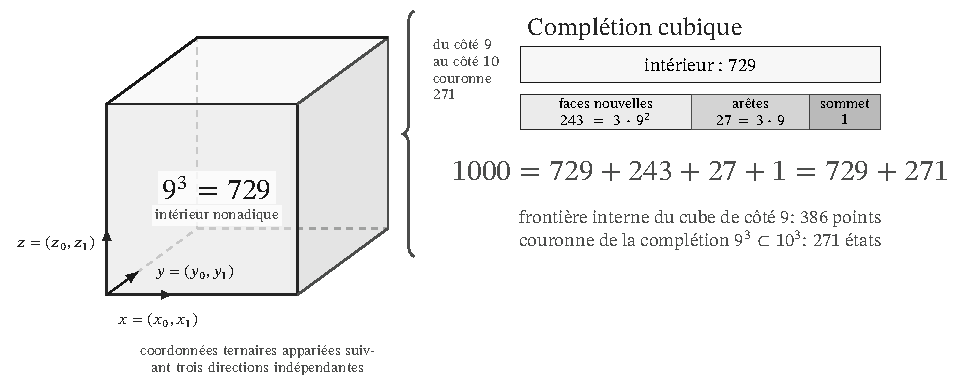
\includegraphics[width=\linewidth]{figures/cubo_emrh.pdf}
\caption{Représentation cubique de l'extension de neuf à dix classes par coordonnée. Les strates \(S_1,S_2,S_3\) placent les incidences ajoutées sur les faces, les arêtes et l'apex ; leurs cardinaux forment la couronne de \(271\) éléments. La frontière de \(386\) éléments appartient au cube initial. La perspective géométrique complète la partition de la figure ~\ref{fig:revision-emrh} ; les séparations graphiques ont une fonction schématique.}
\label{fig:completacion-cubo-recuperado}
\end{figure}


\subsubsection{Conservation de l'unité et compatibilité dimensionnelle}

La normalisation ne se limite pas à diviser une identité isolée. En dimension
\(d\), le produit \(\widehat E^d\) porte la mesure uniforme
\(\mu_d(\{x\})=10^{-d}\). La projection coordonnée
\(p_d:\widehat E^{d+1}\to\widehat E^d\) supprime la dernière coordonnée.

\begin{proposition}[Compatibilité projective des mesures normalisées]
Pour tout \(d\geq1\),
\[
 (p_d)_*\mu_{d+1}=\mu_d,
 \qquad \mu_d(\widehat E^d)=1.
\]
La masse de la strate comportant \(r\) coordonnées supplémentaires est
\(\binom dr9^{d-r}/10^d\), et la somme des masses de toutes les strates
vaut un.
\end{proposition}
\begin{proof}
Chaque point de \(\widehat E^d\) possède dix préimages. Leur masse totale est
\(10\,10^{-(d+1)}=10^{-d}\). L'égalité pour tout sous-ensemble
s'obtient en sommant sur ses points. La formule stratifiée provient
du même dénombrement que \eqref{eq:revision-estratos} ; le binôme
\((9+1)^d\) donne la normalisation totale.
\end{proof}

En dimension trois, retirer l'apex laisse une masse \(999/1000\), et
le restituer ajoute \(1/1000\). Renormaliser avant la restitution
définirait une autre mesure : la distinction est pertinente sur le plan opératoire.
En particulier, conservation de la masse probabiliste, conservation des
registres de transport et dissipation thermodynamique sont des affirmations portant sur
des objets différents. La proposition démontre la première et fournit le
support compatible pour étudier la deuxième ; la troisième requiert une
réalisation dynamique et énergétique spécifiée.

La frontière géométrique interne demeure également distincte.
Sur le représentant cartésien \(\{1,\ldots,9\}^3\), retirer
\(\{2,\ldots,8\}^3\) laisse \(386\) points. Cette frontière appartient au
cube initial, tandis que \(\widehat C\setminus C\) appartient à son
extension. La complétion cubique, le développement positionnel en base mille et
la lecture d'incidence exceptionnelle partagent des données du support ;
leurs applications respectives déterminent l'information issue de ces données qu'utilise
chaque représentation.


\subsection{Incidence cubique et réalisation lorentzienne}

La complétion cubique apporte une relation entre intérieur et frontière.
Sa géométrie peut être développée au moyen de l'incidence des six faces
avec les huit sommets. Étiquetons les faces par \((i,\varepsilon)\),
\(i\in\{1,2,3\}\), \(\varepsilon\in\{+1,-1\}\), et les sommets par
\(\nu\in\{+1,-1\}^3\). La matrice d'incidence est
\[
 M_{(i,\varepsilon),\nu}=\mathbf1_{\{\nu_i=\varepsilon\}}.
\]
Soient \(u=(1,\ldots,1)^{\mathsf T}\in\RR^6\), \(R_F\) l'opposition des faces et \(P_u=uu^{\mathsf T}/6\), \(P_-=(I-R_F)/2\).

\begin{proposition}[Quotient d'incidence de dimension quatre]
Le gramien d'incidence satisfait
\[
 MM^{\mathsf T}=12P_u+4P_-.
\]
Ses valeurs propres \(12,4,0\) ont les multiplicités \(1,3,2\).
En conséquence,
\[
 Q_\square=\RR^6/\ker(MM^{\mathsf T})
 \simeq\RR u\oplus E_-,\qquad E_-=\operatorname{im}P_-.
\]
\end{proposition}
\begin{proof}
Une face contient quatre sommets ; deux faces opposées ont une intersection vide, et deux faces distinctes non opposées partagent deux sommets. La matrice \(12P_u+4P_-\) possède précisément ces entrées. L'espace uniforme est de dimension un ; les différences entre faces opposées engendrent un espace de dimension trois, orthogonal à l'espace uniforme. Son complément est de dimension deux et appartient au noyau.
\end{proof}

La décomposition \(1+3\) procède de l'incidence. Le choix temporel
est déclaré au moyen de la forme bilinéaire
\[
 B_\square([x],[y])=\langle x,(P_--P_u)y\rangle.
\]
Elle est bien définie sur le quotient, car les deux projecteurs annulent le
noyau. Dans la base
\[
 t=[u]/\sqrt6,\qquad
 d_i=[e_{i,+}-e_{i,-}]/\sqrt2,
\]
sa matrice est \(\operatorname{diag}(-1,1,1,1)\). Sont ainsi explicités
le domaine, la décomposition et la convention de signe qui produisent
la réalisation de Minkowski. Le gramien positif détermine le quotient ;
l'affectation temporelle détermine la forme indéfinie sur celui-ci.

L'opérateur
\[
 W_\square=\sqrt6P_u+\sqrt2P_-,\qquad
 W_\square e_{i,\varepsilon}=t+\varepsilon d_i
\]
envoie les six étiquettes de face sur des directions nulles, puisque
\(B_\square(t+\varepsilon d_i,t+\varepsilon d_i)=-1+1=0\).
L'inversion d'une direction et l'opposition des faces disposent ainsi
d'une réalisation géométrique concrète.

\subsubsection{Soudure, inversion et subdivision}

La réalisation cellulaire utilise un transport inversible \(U_m(a)\),
qui conserve la forme lorentzienne, entre les fibres aux extrémités d'une
arête duale orientée \(a\), une étiquette
de face \(\lambda_m(a)\) et une orientation \(\sigma_m(a)\).
Avec \(\ell_m=\ell_0/9^m\), l'application de soudure est
\[
 \beta_m(a)=\ell_m\sigma_m(a)
 W_{\square,s(a)}e_{\lambda_m(a)}.
\]
L'inversion compatible satisfait
\[
 \beta_m(\bar a)=-U_m(a)\beta_m(a).
\]
Identifions les fibres de l'origine à deux niveaux consécutifs au moyen de l'isométrie de raffinement déclarée. Si les neuf sous-segments \(a_1,\ldots,a_9\), de niveau \(m+1\), conservent leur étiquette et leur orientation lorsqu'ils sont transportés vers cette fibre commune, alors
\begin{equation}
 \beta_m(a)=\sum_{j=1}^9
 U_{m+1}(a_1\cdots a_{j-1})^{-1}\beta_{m+1}(a_j).
 \label{eq:soldadura-refinamiento}
\end{equation}
Chaque terme transporté équivaut à \(\ell_m/9\) suivant la même
direction nulle, ce qui démontre l'identité. L'hypothèse de
compatibilité détermine quelles subdivisions réalisent ce raffinement.
L'équation réunit direction, échelle et transport, au lieu de limiter
la correspondance géométrique à un dénombrement des dimensions.

L'orientation et la forme lorentzienne étant également fixées, la dualité de Hodge dans \(\Lambda^2Q_\square^*\) satisfait \(\star^2=-I\). En dimension quatre, le signe est \((-1)^{2(4-2)+1}=-1\). On obtient une structure complexe réelle sur les deux-formes et, après complexification, les sous-espaces propres de valeurs \(+i\) et \(-i\). La réalisation électromagnétique utilisera ce domaine après la construction de la section électronique et la déclaration de son couplage.

\subsection{Compatibilité entre les réductions modulaire et positionnelle}

La base décimale par blocs intervient au moyen d'une division euclidienne
qui conserve simultanément le résidu et le quotient :
\[
 n=1000q+r,\qquad 0\le r<1000.
\]
Puisque \(1000\equiv1\pmod9\) et \(1000\equiv1\pmod3\),
\[
 n\equiv q+r\pmod9,\qquad n\equiv q+r\pmod3.
\]
Par conséquent, la réduction d'un bloc requiert la contribution du
quotient pour restituer la classe de l'entier. Les nombres \(0\) et
\(1000\) ont le même reste modulo \(1000\), mais des classes différentes
modulo \(9\) et modulo \(3\). C'est une raison opératoire de conserver
la mémoire pendant le changement de résolution.

Le raffinement ternaire et la détermination d'un préfixe décimal
peuvent se coordonner au moyen d'un unique résidu entier. Si \(N/3^L\)
est une extrémité de cylindre et \(D/1000^r\) une extrémité décimale, nous définissons
\[
 A=1000^rN-D3^L.
\]
En ajoutant six symboles ternaires, \(N'=729N+\nu\),
\(L'=L+6\), avec \(0\le\nu<729\). Si le préfixe décimal reste
fixe, on obtient
\[
 A'=729A+\nu1000^r.
\]
Si l'on incorpore en outre un bloc décimal \(\delta\), alors \(D'=1000D+\delta\), \(r'=r+1\), et
\begin{equation}
 A'=729000A+\nu1000^{r+1}-729\delta3^L.
 \label{eq:residuo-dos-bases}
\end{equation}
Les deux identités se démontrent en substituant les définitions. La
comparaison des extrémités se réduit ainsi à des opérations entières qui
retiennent la contribution de chaque prolongation. Cette compatibilité
permet de raffiner une région avant d'évaluer sa coordonnée réelle.

% Incorporación al final de extension.tex; no contiene una sección principal.
% Procedencia: RESULTADO_RECUPERADO; explicitación sectorial de las hipótesis.
% Fuentes leídas: monografía Doble proyección holográfica (cantera editorial),
% manuscrito/local/01_tesis_recuperada.tex y
% manuscrito/generated/algebra_holonomica.tex, especialmente §§1--7 y 21.
% Definición rectora de número: manuscrito/flattened/main_autosuficiente.tex,
% secciones que comienzan en líneas 22137 y 23000 de la cantera de 775 páginas.
% No se adopta su presentación global como prueba de todas las flechas TPK.

\subsection{Le nombre comme section compatible et la valeur comme lecture}
\label{hist:seccion}

La distinction entre état et observation permet de préciser quel objet se
prolonge lorsque la résolution augmente. À la profondeur \(n\), soit \(X_n\)
l’ensemble des états admissibles produits par APP--TRIT--TPK. Leurs données
comprennent la position, les feuillets somme et produit, les résidus et les quotients, le régime,
l’orientation, la retenue, la phase, la route, la frontière, la mémoire et la survie. Ce ne sont pas
des coordonnées indépendantes : les évaluations arithmétiques et les transports
précédents imposent leurs relations. Un prolongement conserve ces relations
dans chaque antécédent, tout en ajoutant de nouvelles étapes et de nouvelles données de mémoire.
Tel est le sens de l’arithmétique des histoires développée dans
(sections~\ref{sec:extension} et~\ref{mono-ampl:conexion}).

Soient \(r_{m,n}:X_m\to X_n\), pour \(m\geq n\), les restrictions de
profondeur, avec \(r_{n,n}=\operatorname{id}\) et
\(r_{\ell,n}=r_{m,n}\circ r_{\ell,m}\). Chaque restriction conserve le
préfixe et l’information déjà déterminée en lui.

\begin{definition}[Section numérique compatible]
Un nombre HMT est une histoire compatible du système d’états :
\begin{equation}
 x=(x_n)_{n\geq0}\in X_\infty:=\varprojlim_n X_n,
 \qquad r_{m,n}(x_m)=x_n.
 \label{hist:limite-inverso}
\end{equation}
Un lecteur est une opération supplémentaire sur un domaine spécifié de ces
histoires. Un chiffre est une observation finie ; une valeur scalaire est une
évaluation du lecteur. Le couple formé de la section et de son lecteur constitue
une présentation munie d’une lecture, non une redéfinition de l’identité de la section.
\end{definition}

Dans le domaine archimédien \(X_\infty^{\mathrm{Arch}}\), le lecteur associe
à chaque préfixe un cylindre fermé, conserve leur emboîtement et fait tendre
leur diamètre vers zéro. Il détermine ainsi
\begin{equation}
 \operatorname{ev}_{\mathbb R}:X_\infty^{\mathrm{Arch}}\longrightarrow
 \mathbb R,\qquad
 \{\operatorname{ev}_{\mathbb R}(x)\}=\bigcap_n I_n(x).
 \label{hist:evaluacion}
\end{equation}
La construction concrète de ces cylindres et la décision de leurs frontières
sont développées dans la section~\ref{sec:generacion}. La définition
\eqref{hist:limite-inverso} n’affirme pas à elle seule que l’image de
\eqref{hist:evaluacion} soit la droite entière : une affirmation de couverture
requiert son propre théorème. Une égalité de valeurs n’établit pas non plus, sans
résultat d’injectivité, l’égalité de leurs histoires. Cette séparation
permet de parler de précision comme profondeur en conservant la différence
entre l’antécédent arithmétique et sa réalisation scalaire.

\subsection{Composition des histoires et multiplicateur de mémoire}
\label{hist:algebra}

Fixons un secteur d’états à la profondeur \(n\) et une catégorie
\(\mathcal C\) dont les flèches sont leurs histoires admissibles. La composition
s’écrit \(vu=v\circ u\) : on parcourt d’abord \(u\), puis \(v\).
Les pas élémentaires proviennent de la sélection, du transport et de
l’actualisation du TPK. Une fibre tritique locale admet l’écriture
\(\mathbb R[J_x]/(J_x^2+\tau(x)1_x)\), où
\(\tau(x)\in\{+1,0,-1\}\). Le régime et l’orientation appartiennent à
l’état transporté ; une transition entre régimes n’équivaut pas à
l’identification de leurs algèbres quadratiques.

La formulation suivante précise un secteur algébrique de cette composition.
Pour chaque objet \(x\), on se donne une algèbre réelle associative unitaire \(A_x\),
éventuellement non commutative. Pour chaque \(u:x\to y\), on se donne un
homomorphisme unital \(\rho_u:A_x\to A_y\). Nous supposons une action stricte :
\begin{equation}
 \rho_{\operatorname{id}_x}=\operatorname{id}_{A_x},\qquad
 \rho_v\rho_u=\rho_{vu}.
 \label{hist:accion-estricta}
\end{equation}
Pour chaque couple composable \(u:x\to y\), \(v:y\to z\), nous fixons un
multiplicateur central inversible
\(\Omega(v,u)\in Z(A_z)^\times\). On exige la normalisation
\(\Omega(\operatorname{id}_y,u)=\Omega(u,\operatorname{id}_x)=1_y\)
et, pour chaque triplet composable, l’identité
\begin{equation}
 \rho_w\bigl(\Omega(v,u)\bigr)\Omega(w,vu)
   =\Omega(w,v)\Omega(wv,u).
 \label{hist:cociclo}
\end{equation}
Il s’agit d’hypothèses explicites sur les transports et leurs coefficients, non d’une
conséquence du qualificatif holonomique appliqué à la dynamique. Pour appliquer cette présentation
à un secteur TPK, il faut identifier ses \(\rho_u\) et \(\Omega(v,u)\).
Les transitions exprimées par des bimodules exigent la conservation de cette
structure et ne sont pas remplacées par \eqref{hist:accion-estricta}.

L’espace des sommes finies
\[
 \mathcal H(\mathcal C,A,\rho,\Omega)
   =\bigoplus_{u\in\operatorname{Mor}(\mathcal C)} A_{t(u)}T_u
\]
est muni du produit bilinéaire
\begin{equation}
 (aT_v)(bT_u)=a\rho_v(b)\Omega(v,u)T_{vu},
 \label{hist:producto}
\end{equation}
si les flèches sont composables, et de zéro sinon. Ici, \(t(u)\)
désigne l’état terminal. La somme réunit des histoires à coefficients ; le
produit concatène les histoires en conservant le multiplicateur du registre.

\begin{proposition}[Associativité sectorielle à multiplicateur central]
Sous \eqref{hist:accion-estricta} et \eqref{hist:cociclo}, le produit
\eqref{hist:producto} est associatif. Si l’ensemble des objets est fini,
son unité est \(\sum_x1_xT_{\operatorname{id}_x}\).
\end{proposition}
\begin{proof}
Pour \(u:x\to y\), \(v:y\to z\), \(w:z\to t\), soient
\(a\in A_y\), \(b\in A_z\), \(c\in A_t\). Les deux coefficients
de \(T_{wvu}\) sont
\begin{align*}
 ((cT_w)(bT_v))(aT_u):\quad&
 c\rho_w(b)\Omega(w,v)\rho_{wv}(a)\Omega(wv,u),\\
 (cT_w)((bT_v)(aT_u)):\quad&
 c\rho_w(b)\rho_w\rho_v(a)\rho_w(\Omega(v,u))\Omega(w,vu).
\end{align*}
L’action stricte identifie \(\rho_w\rho_v(a)\) à \(\rho_{wv}(a)\).
La centralité de \(\Omega(w,v)\) permet de le déplacer à droite de
ce facteur ; \eqref{hist:cociclo} égalise alors les produits restants.
Les coefficients \(a,b,c\) ne sont pas permutés. Si le triplet n’est pas composable,
les deux parenthésages sont nuls du fait de leurs états initiaux et terminaux.
La bilinéarité achève la preuve. Les identités locales et la
normalisation de \(\Omega\) vérifient l’unité indiquée.
\end{proof}

La retenue du calendrier fournit un exemple effectif. Dans la catégorie
à un objet et de flèches \(C_9\), prenons pour coefficients
\(A=\mathbb R[z,z^{-1}]\), l’action identité et
\[
 \Omega(b,a)=z^{c_0(a,b)},\qquad
 c_0(a,b)=\left\lfloor\frac{a+b}{9}\right\rfloor,
 \quad 0\leq a,b<9.
\]
Les deux sommes de retenues d’un triplet sont
\(\lfloor(a+b+c)/9\rfloor\) ; \eqref{hist:cociclo}
est donc satisfaite. La variable formelle \(z\) enregistre le tour sans
lui attribuer de valeur numérique. Imposer ensuite \(z^{12}=1\) restitue le
registre dodécaphasique du calendrier \eqref{eq:extension108} ; conserver
\(z\) sans cette relation distingue les tours successifs. L’exemple réalise
la mémoire de ce calendrier, sans l’identifier à la totalité de la
mémoire TPK.

\subsection{Double variance du raffinement et conservation de l’unité}
\label{hist:doble-varianza}

La restriction des états prolonge les observables en sens contraire.
Considérons les algèbres de fonctions, munies du produit ponctuel,
\(D_n=\operatorname{Fun}(X_n,\mathbb R)\). La précomposition définit
\begin{equation}
 r_{m,n}^*:D_n\longrightarrow D_m,
 \qquad r_{m,n}^*f=f\circ r_{m,n}.
 \label{hist:precomposicion}
\end{equation}
Ce sont des morphismes unitaux ; ils sont également injectifs lorsque les restrictions
correspondantes sont surjectives. La limite inductive
\(D_{\mathrm{cyl}}=\varinjlim_n(D_n,r_{n+1,n}^*)\) réunit les
observations de profondeur finie. Cette algèbre n’est pas identifiée ici
à l’algèbre entière des routes : prolonger les opérateurs de transport exige
également leurs compatibilités avec le raffinement.

\begin{lemma}[Unité et naturalité de l’évaluation]
Si \(e_x\) est l’indicatrice de \(x\in X_n\), on a
\begin{equation}
 r_{m,n}^*e_x=\sum_{y:\,r_{m,n}(y)=x}e_y,
 \qquad r_{m,n}^*1_n=1_m,
 \label{hist:unidad}
\end{equation}
et, pour tous \(f\in D_n\), \(y\in X_m\),
\[
 \langle r_{m,n}^*f,y\rangle=\langle f,r_{m,n}y\rangle.
\]
Chaque section \(x\in X_\infty\) détermine une évaluation bien définie
\(D_{\mathrm{cyl}}\to\mathbb R\), donnée par \([f]\mapsto f(x_n)\)
pour \(f\in D_n\).
\end{lemma}
\begin{proof}
Les fibres de \(r_{m,n}\) forment une partition de \(X_m\). Leurs
indicatrices sont orthogonales et de somme \(1_m\), ce qui démontre
\eqref{hist:unidad}. La naturalité est la définition de la précomposition.
Enfin, \((r_{m,n}^*f)(x_m)=f(x_n)\), de sorte que deux représentants
compatibles donnent la même évaluation dans la limite inductive.
\end{proof}

L’unité globale est la fonction constante un sur toutes les possibilités ;
la section individuelle sélectionne une histoire compatible. Conserver la
première ne signifie pas immobiliser la seconde. Le raffinement peut augmenter
le nombre d’extensions et la profondeur de chaque histoire en maintenant
l’unité et toutes les évaluations de ses antécédents.

\subsection{Retour de phase, représentation de Weyl et deux lectures}
\label{hist:puente-lecturas}

La loi \eqref{eq:holonomia-memoria} acquiert une réalisation opératorielle
dans la suspension bilatérale qui sera construite dans la
section~\ref{sec:generacion}. Dans celle-ci, \(T\) est l’avancement d’un pas,
\(V_9\) observe la phase nonadique, \(W_\delta\) la phase de rotation et
\(D_M\) le degré de mémoire. En écrivant
\(\widehat\Gamma_9=T^9\) pour le tour dans cette représentation,
les relations de Weyl \eqref{eq:weyl-relojes} impliquent, sur les vecteurs
de support fini,
\begin{equation}
 \begin{aligned}
 V_9\widehat\Gamma_9&=\widehat\Gamma_9V_9,\qquad
 W_\delta\widehat\Gamma_9=e^{2\pi i9\delta}
     \widehat\Gamma_9W_\delta,\\
 [D_M,\widehat\Gamma_9]&=\widehat\Gamma_9.
 \end{aligned}
 \label{hist:tres-retornos}
\end{equation}
La première égalité découle de \(\zeta_9^9=1\) ; la deuxième, de neuf
applications de la covariance de \(W_\delta\) ; la troisième exprime
l’incrément unitaire de mémoire. La phase finie revient, tandis que la
rotation irrationnelle et la mémoire distinguent l’état suivant. Les
caractères et le paramètre \(\delta\) sont réalisés ultérieurement à partir de la
construction numérique spécifiée dans cette section : ils ne sélectionnent pas rétrospectivement
les conditions initiales. Cette représentation décrit les observables et les translations de
la suspension ; elle ne remplace ni toutes les coordonnées ni tous les opérateurs
du TPK.

La double lecture prolonge la même distinction entre histoire et observable.
Dans son domaine archimédien, on applique \eqref{hist:evaluacion} ; dans le
domaine d’incidence calibré, les applications \(Q_n\) de la
section~\ref{exc:doble-lectura} conservent les mots et les repères de
frontière. L’égalité qui y est démontrée,
\(r_{n,m}Q_n=Q_mp_{n,m}\), détermine leur prolongement \(Q_\infty\).
Sur le domaine commun aux deux lectures, on peut considérer conjointement
\(\operatorname{ev}_{\mathbb R}(x)\) et \(Q_\infty(x)\) : la
première retient la valeur ; la seconde, l’incidence transportée que son
codomaine conserve. La section précède les deux. Cette articulation permet
de passer de l’arithmétique des histoires aux constantes et à la lecture
exceptionnelle sans transformer leurs réalisations en nouvelles données initiales.


\section{Construction corrélative du continu : histoires, transport, incidence et terminal}
\label{iv:continuo-conjunto}
L’arithmétique exprimée par une forme normale conserve une lecture précise de l’état qui la produit. Pour situer cette lecture dans HMT, il est nécessaire de maintenir aussi les histoires, les feuillets et les opérations qui agissent sur eux. Ce chapitre réunit ce substrat commun. Ses différentes constructions s’obtiennent à partir du même arbre d’exécutions APP–TRIT–TPK ; les découpages de l’exposition permettent d’étudier leurs propriétés sans les transformer en domaines indépendants choisis par une application ultérieure.

Le point de départ est le noyau formel exposé précédemment. Une émission admissible contient l’opération de APP, l’orientation du TRIT, le changement de feuillet, le résidu et le quotient, ainsi que la mise à jour effective de mémoire du TPK. Lorsque seul un résidu est exprimé, l’histoire d’exécution appartient toujours à l’objet de départ. Deux exécutions ayant une lecture finale identique ne sont pas identifiées pour ce seul motif.

\subsection{Histoires admissibles et mémoire par composition}
\label{iv:cont:historias}
Soit \(X_k\) l’ensemble des histoires admissibles de longueur \(k\). Ses éléments sont construits par émissions successives à partir du domaine initial du noyau. Nous écrivons \(h\varepsilon\) pour le prolongement de \(h\) par une émission admissible \(\varepsilon\), et \(\rho_k(h\varepsilon)=h\) pour la suppression de la dernière émission. L’étiquette de l’émission est conservée, même lorsque des étiquettes différentes produisent un même état exprimé.

Dans les deux feuillets arithmétiques, les données locales satisfont les divisions exactes

\[
\delta_\diamond=r_\diamond+9q_\diamond,
\qquad 0\leq r_\diamond<9,
\qquad \diamond\in\{\Sigma,\Pi\}.
\]
La coordonnée orientée du TRIT admet, de manière analogue, une écriture \(\Delta=o_r+3\kappa\), avec le représentant orienté déclaré par le noyau. La conservation du quotient permet de composer ces représentations sans remplacer une émission par son résidu isolé.

Dans un système de coordonnées de mémoire, la mise à jour d’une émission s’écrit

\[
U_\varepsilon(m)=C_\varepsilon m+\kappa_\varepsilon.
\]
Pour une trajectoire \(\alpha=(\varepsilon_1,\ldots,\varepsilon_k)\), l'opération effective est la composition ordonnée de ces mises à jour. Sa partie linéaire et sa translation sont

\[
C_\alpha=C_{\varepsilon_k}\cdots C_{\varepsilon_1},
\qquad
\kappa_\alpha=
\sum_{j=1}^{k}C_{\varepsilon_k}\cdots
C_{\varepsilon_{j+1}}\kappa_{\varepsilon_j}.
\]
Le produit vide de la dernière somme est l'identité.

\begin{proposition}[Compatibilité affine de la concaténation]
\label{iv:cont:concatenacion}
Si \(\alpha\) précède \(\beta\), alors

\[
C_{\beta\alpha}=C_\beta C_\alpha,
\qquad
\kappa_{\beta\alpha}=C_\beta\kappa_\alpha+\kappa_\beta,
\qquad
U_{\beta\alpha}=U_\beta U_\alpha.
\]
\end{proposition}
\begin{proof}
Substituer \(U_\alpha(m)\) dans \(U_\beta\) produit \(C_\beta C_\alpha m+C_\beta\kappa_\alpha+\kappa_\beta\). La décomposition en partie linéaire et translation donne les trois identités. L'associativité de la composition démontre que le résultat ne dépend pas d'une subdivision auxiliaire de la trajectoire.
\end{proof}

Cette identité de cocycle est le contenu précis de la mémoire accumulée. La quantité transportée par une seconde trajectoire dépend de la mise à jour du système de coordonnées qu’elle réalise ; ce n’est pas, en général, la somme sans transport de deux registres.

Le retour nonadique conserve une seconde distinction. Dans les coordonnées de phase et de tour, avec \(\bar r\in\{0,\ldots,8\}\), sa représentation est

\[
\sigma_9(w,r)=
\left(w+\left\lfloor\frac{\bar r+1}{9}\right\rfloor,
r+1\pmod9\right),
\qquad
\sigma_9^9(w,r)=(w+1,r).
\]
Pendant neuf étapes, il se produit exactement un franchissement de \(8\) à \(0\). La phase revient et la coordonnée de tour augmente. L'holonomie enrichie retient en outre les mises à jour de mémoire qui accompagnent ce parcours.

\subsection{Raffinement de l'arbre et mesure des histoires}
\label{iv:cont:medida}
On fixe l’ensemble initial fini non vide de germes admissibles, avec une masse initiale strictement positive et de somme \(1\). Dans ce paragraphe, chaque histoire a un nombre fini et positif de prolongements. La suppression d’émissions définit les applications de raffinement. L’admissibilité du noyau fournit les prolongements ; lorsqu’une résidence utilise une émission neutre, celle-ci donne explicitement une section de \(\rho_k\). L’existence de cette section se rapporte à l’arbre qui comprend cette émission, non à toute restriction arbitraire de routes.

Soit \(d(h)\geq1\) le nombre d’émissions admissibles dans \(h\). Le choix équiprobable parmi ses successeurs définit

\[
\mu(h\varepsilon)=\frac{\mu(h)}{d(h)}.
\]
Plus généralement, une distribution locale positive \(p(\varepsilon\mid h)\), dont la somme est \(1\), définit \(\mu(h\varepsilon)=\mu(h)p(\varepsilon\mid h)\). Cette seconde formulation permet de conserver les pondérations du lecteur lorsque les nombres de prolongements ne sont pas uniformes.

\begin{proposition}[Compatibilité cylindrique et espérance conditionnelle]
\label{iv:cont:esperanza}
À chaque niveau, on a

\[
\sum_{\rho_k(y)=x}\mu(y)=\mu(x).
\]
Dans les espaces \(L^2(X_k,\mu_k)\), les applications

\[
(J_kf)(y)=f(\rho_k(y)),
\qquad
(E_kg)(x)=\sum_{\rho_k(y)=x}\frac{\mu(y)}{\mu(x)}g(y)
\]
satisfont \(E_k=J_k^*\), \(E_kJ_k=I\) et \(\|J_kf\|=\|f\|\).

\end{proposition}
\begin{proof}
La première identité est la normalisation des probabilités locales. En l’appliquant à \(|f(x)|^2\), on obtient l’isométrie. En regroupant par prédécesseurs la somme qui définit \(\langle J_kf,g\rangle\), on obtient la formule de \(E_k\) ; sur une fonction constante dans chaque fibre, cette formule renvoie sa valeur.
\end{proof}

Les masses compatibles définissent une mesure de probabilité sur l’espace des histoires infinies : le cylindre d’une histoire finie reçoit sa masse \(\mu(h)\). La mesure s’étend à partir de l’algèbre des cylindres, et son unicité découle du fait que ceux-ci engendrent la tribu. Si l’arbre est à ramifications finies et si chaque histoire possède un prolongement, la limite projective de ses niveaux par suppression d’émissions est non vide. Dans la topologie cylindrique, chaque cylindre non vide est de mesure positive.

Cette mesure distingue les histoires qui convergent vers une même représentation. La mesure uniforme sur les valeurs terminales serait une lecture différente, car elle éliminerait les multiplicités que la construction vient de conserver.

\subsection{Transport par feuillets et comptabilité exacte des sorties}
\label{iv:cont:transporte}
Considérons d’abord l’espace dont la base orthonormée est formée par les histoires du niveau \(k\). Le transport qui conserve l’étiquette de chaque prolongement est

\[
\mathcal U_ke_h=
\sum_{\varepsilon\ \mathrm{admissible\ en}\ h}
\sqrt{p(\varepsilon\mid h)}\,e_{h\varepsilon}.
\]
Les ensembles de successeurs de prédécesseurs distincts sont disjoints. La normalisation de \(p\) démontre donc \(\mathcal U_k^*\mathcal U_k=I\). La représentation au moyen des masses d’histoires est reliée à celle-ci par le changement de base diagonal qui incorpore \(\sqrt{\mu(h)}\).

L'étiquette de feuillet fait partie du registre complet d'une histoire. On écrit
\[
\widehat h=((h_0,s_0),\ldots,(h_k,s_k)),\qquad
s_j\in\{\Sigma,\Pi\},
\]
où \(s_j\) est le feuillet actif à l'étape \(j\). La prolongation ajoute l'émission et le feuillet \(s_{k+1}\) déterminé par le sélecteur opératoire du TPK, en conservant le préfixe intégralement, y compris le feuillet initial. Dans la base de ces histoires relevées,
\[
\mathcal U_ke_{\widehat h}
=\sum_{\varepsilon\ \mathrm{admissible\ en}\ \widehat h}
\sqrt{p(\varepsilon\mid\widehat h)}\,e_{\widehat h\varepsilon},
\qquad
P_ke_{\widehat h}=\mathbf1_{s_k=\Sigma}e_{\widehat h},\quad
Q_k=I-P_k.
\]
Ainsi, \(P_k\) lit le feuillet actuel, tandis que la distinction entre histoires est maintenue par leur préfixe complet. Deux histoires initiales qui parviennent au même feuillet actif continuent d’avoir des successeurs distincts. La preuve d’isométrie par collections disjointes de prolongements s’applique littéralement à cette base.
L’orientation tritique est une autre coordonnée du registre : la valeur \(0\) conserve la lecture de seuil dans chaque feuillet et n’ajoute pas de troisième feuillet à cette décomposition. Nous séparons maintenant la conservation du feuillet et l’échange de feuillet :

\[
A_k=P_{k+1}\mathcal U_kP_k+Q_{k+1}\mathcal U_kQ_k,
\qquad
\eta_k=Q_{k+1}\mathcal U_kP_k+P_{k+1}\mathcal U_kQ_k.
\]
\begin{proposition}[Identité de Gram par feuillets]
\label{iv:cont:gram}
Pour un transport linéaire \(U\), isométrique ou non, la décomposition précédente satisfait

\[
A^*A+\eta^*\eta=PU^*UP+QU^*UQ.
\]
En particulier, pour \(U=\mathcal U_k\),

\[
A_k^*A_k+\eta_k^*\eta_k=I.
\]
\end{proposition}
\begin{proof}
Dans \(A^*A\) et \(\eta^*\eta\), les termes mixtes contenant \(P_{k+1}Q_{k+1}\) s'annulent. En additionnant les termes restants apparaît \(P_kU^*(P_{k+1}+Q_{k+1})UP_k\), ainsi que son analogue avec \(Q_k\). La première identité résulte de la complémentarité des projecteurs ; la seconde utilise en outre \(U^*U=I\).
\end{proof}

La première identité est la formule générale. Remplacer son membre de droite par \(U^*U\) requiert l'annulation des blocs croisés de ce gramien. La conservation isométrique du transport des histoires fournit ici cette condition ; elle ne doit pas être attribuée automatiquement à une compression ultérieure.

Écrivons \(F_{0,0}=I\), \(F_{0,n}=A_{n-1}\cdots A_0\) et \(T_N=F_{0,N}^*F_{0,N}\).

\begin{theorem}[Décomposition finie avec résidu terminal]
\label{iv:cont:terminal}
Pour chaque horizon \(N\),

\[
I=\sum_{n=0}^{N-1}
F_{0,n}^*\eta_n^*\eta_nF_{0,n}+T_N.
\]
La suite \(T_N\) est positive et décroissante, et possède une limite forte positive \(T_\infty\). La somme des sorties converge fortement vers \(I-T_\infty\).

\end{theorem}
\begin{proof}
La proposition~\ref{iv:cont:gram} donne \(T_n-T_{n+1}=F_{0,n}^*\eta_n^*\eta_nF_{0,n}\). La somme télescopique prouve l'égalité finie et la monotonie. Pour chaque vecteur, les formes quadratiques décroissent vers une limite ; la polarisation définit une forme bornée positive et, par le théorème de représentation des formes bornées, un opérateur \(T_\infty\). La convergence est forte parce que, pour un opérateur positif \(S\leq I\), \(\|Sv\|^2\leq\langle v,Sv\rangle\) ; on l'applique à \(S=T_N-T_\infty\).
\end{proof}

Le résidu terminal est conservé jusqu'à la démonstration de son extinction dans le domaine considéré. Cette distinction empêche qu'un retour de phase, à lui seul, se transforme en une hypothèse d'épuisement de toutes les histoires.

\subsection{Bilan orienté et annulation dans le raffinement}
\label{iv:cont:balance}
Une histoire porte son orientation accumulée \(o(h)\) et les dénombrements de ses visites aux deux feuillets. Le bilan local correspondant est

\[
b(h)=o(h)\bigl(N_\Sigma(h)-N_\Pi(h)\bigr),
\qquad
b^+=\frac{|b|+b}{2},\quad b^-=\frac{|b|-b}{2}.
\]
Lorsqu’un lecteur exprime la moyenne sur les prolongements, on définit \(b_c=Eb_f\). L’orientation reste dans l’argument de \(b_f\) ; elle n’est pas éliminée avant le calcul de la moyenne.

\begin{proposition}[Défaut exact d'annulation]
\label{iv:cont:cancelacion}
La quantité

\[
\kappa_{\mathrm{can}}=
\frac{E|b_f|-|Eb_f|}{2}
\]
est non négative et satisfait

\[
E(b_f^+)=(b_c)^++\kappa_{\mathrm{can}},
\qquad
E(b_f^-)=(b_c)^-+\kappa_{\mathrm{can}}.
\]
\end{proposition}
\begin{proof}
L'inégalité triangulaire pondérée donne \(|Eb_f|\leq E|b_f|\). En écrivant les parties positive et négative au moyen de \((|b|\pm b)/2\), on obtient les deux égalités.
\end{proof}

L’information omise lorsque seul le bilan est exprimé est l’annulation commune des contributions opposées. Cette quantité est déterminée à partir des mêmes prolongements utilisés par le transport précédent. Le facteur \(1/9\) n’apparaît que lorsque la fibre contient neuf successeurs de poids égaux ; l’espérance conditionnelle est la règle qui reste valable pour une ramification et des pondérations générales.

\subsection{Incidence ternaire des feuillets et complexe rectangulaire}
\label{iv:cont:incidencia-rectangular}
Les deux feuillets déterminent le module \(V=\mathbb F_3e_\Sigma\oplus\mathbb F_3e_\Pi\). Ses quatre directions projectives sont les droites engendrées par \(e_\Sigma,e_\Pi,e_\Sigma+e_\Pi,e_\Sigma-e_\Pi\). Il en provient six couples non ordonnés. Les huit vecteurs non nuls sont leurs représentants orientés. Ainsi, les dénombrements \(4,6,8\) appartiennent à des opérations distinctes sur un même module de feuillets.

Sur les six positions de paires, nous définissons

\[
(Ba)_{\{L,L'\}}=a_L+a_{L'},
\qquad
s(q)=\sum_{\{L,L'\}}q_{\{L,L'\}}.
\]
Chaque direction intervient dans trois paires ; d'où \(sB=0\) dans \(\mathbb F_3\). Le lecteur \(W(q)=\mathbf1_{s(q)=0}-1/3\) est invariant sous \(q\mapsto q+Ba\). Sur l'espace ambiant uniforme \(\mathbb F_3^6\), ses moments sont

\[
\mathbb EW=0,\qquad
\mathbb EW^2=\frac29,\qquad
\mathbb EW^3=\frac2{27}.
\]
En effet, \(s\) est surjective et chaque fibre contient \(3^5\) éléments. Le lecteur vaut \(2/3\) avec la probabilité \(1/3\) et \(-1/3\) avec la probabilité \(2/3\). Ces moyennes décrivent l'espace ambiant uniforme ; la distribution induite par un sous-ensemble d'histoires doit être calculée avec ses propres multiplicités, déjà conservées dans \(X_k\).

Pour fixer les ports sans perdre les multiplicités, à la profondeur \(k\), on conserve les lectures étiquetées \(\lambda_\Sigma(h)=(h,\Sigma)\) et \(\lambda_\Pi(h)=(h,\Pi)\). Leurs ensembles sont
\[
I_k=\{\lambda_\Sigma(h):h\in X_k\},\qquad
J_k=\{\lambda_\Pi(h):h\in X_k\}.
\]
Ils sont finis et non vides parce que \(X_k\) l’est. Les valeurs, les quotients et les résidus sont exprimés sur ces ports ; une égalité de valeurs n’identifie pas leurs étiquettes. Le produit \(I_k\times J_k\) est le domaine de la lecture rectangulaire, à l’intérieur duquel le support des incidences admissibles est enregistré.

Ce niveau étant fixé, nous écrivons \(I=I_k\), \(J=J_k\) et \(A_N=\mathbb Z/3^N\mathbb Z\). Nous choisissons des ports de référence \(i_0,j_0\). Ce choix fournit seulement des coordonnées pour les formules de reconstruction. Les applications

\[
\kappa(u,v)_{ij}=u_i-v_j,
\qquad
(\delta w)_{ij}=w_{ij}-w_{ij_0}-w_{i_0j}+w_{i_0j_0}
\]
définissent la suite suivante, valable sur l'anneau fini \(A_N\) :

\[
0\longrightarrow A_N\longrightarrow
A_N^I\oplus A_N^J\mathrel{\mathop{\longrightarrow}^{\kappa}}
A_N^{I\times J}\mathrel{\mathop{\longrightarrow}^{\delta}}
A_N^{(I\setminus\{i_0\})\times(J\setminus\{j_0\})}
\longrightarrow0.
\]
\begin{proposition}[Exactitude de l'incidence rectangulaire]
\label{iv:cont:rectangular-exacta}
La suite précédente est exacte, avec pour première flèche la diagonale constante.

\end{proposition}
\begin{proof}
L'égalité \(u_i-v_j=0\) pour chaque couple impose que toutes les coordonnées de \(u\) et de \(v\) soient une même constante. La substitution directe donne \(\delta\kappa=0\). Si \(\delta w=0\), prenons \(u_i=w_{ij_0}\) et \(v_j=w_{i_0j_0}-w_{i_0j}\). Alors \(u_i-v_j=w_{ij}\). Enfin, toute matrice du dernier terme se prolonge avec une ligne et une colonne de référence nulles ; son image par \(\delta\) est la matrice initiale. La preuve n'utilise que des sommes et des soustractions ; elle n'exige donc pas de diviser par une unité de l'anneau.
\end{proof}

La réduction de \(A_{N+1}\) à \(A_N\), en maintenant \(k,I_k,J_k,i_0,j_0\) fixes, commute avec les deux applications. Les formules de reconstruction sont les mêmes à chaque profondeur modulaire. Telle est la compatibilité arithmétique démontrée dans ce paragraphe. Le prolongement d’histoires \(k\to k+1\) conserve les étiquettes de préfixe ; ses applications entre ensembles de ports sont une donnée distincte du changement d’anneau \(N\to N+1\).

Ces applications s'obtiennent par la suppression des émissions :
\[
\rho_k^\Sigma(h\varepsilon,\Sigma)=(h,\Sigma),\qquad
\rho_k^\Pi(h\varepsilon,\Pi)=(h,\Pi).
\]
On fixe une histoire de référence à prolongements compatibles, dont l'existence a été démontrée pour l'arbre sans feuilles terminales. Ses deux étiquettes définissent des ports de référence compatibles à tous les niveaux. Le transport des coordonnées est la précomposition :
\[
(L_ku)_{i'}=u_{\rho_k^\Sigma(i')},\quad
(L_kv)_{j'}=v_{\rho_k^\Pi(j')},\quad
(L_kw)_{i'j'}=w_{\rho_k^\Sigma(i'),\rho_k^\Pi(j')}.
\]
Pour le dernier module de la suite, on prolonge d’abord la matrice par zéro dans la ligne et la colonne de référence, on applique cette même formule et on restreint au nouveau complément des ports de référence. Cette règle définit \(L_k\) même lorsqu’un nouveau port a pour prédécesseur le port marqué.

\begin{proposition}[Naturalité du complexe rectangulaire sous prolongement]
\label{iv:rectangular-natural}
Les applications précédentes vérifient
\(L_k\kappa_k=\kappa_{k+1}L_k\) et
\(L_k\delta_k=\delta_{k+1}L_k\).
Elles commutent en outre avec la réduction des coefficients
\(A_{N+1}\to A_N\) et se composent conformément à la suppression des préfixes.
\end{proposition}
\begin{proof}
La première identité s’obtient à partir de
\(u_{\rho_k^\Sigma(i')}-v_{\rho_k^\Pi(j')}\).
Dans la seconde, chacun des quatre termes qui définissent \(\delta\)
est transporté par la même précomposition. La compatibilité des
ports marqués identifie leurs lignes et leurs colonnes ; lorsqu’un prédécesseur est
le port marqué, les quatre termes s’annulent et coïncident avec
le prolongement par zéro. Toutes les formules sont des sommes et des différences à
coefficients entiers, de sorte qu’elles commutent avec la réduction modulaire.
La composition des précompositions est la précomposition par le
préfixe composé, ce qui démontre la dernière affirmation.
\end{proof}

\subsection{Complexe de mémoire et compatibilité des incidences}
\label{iv:cont:memoria}
La même coordonnée accumulée de mémoire \(c_y\in\mathbb Z\), dans une résidence \(y\), définit un complexe libre entier. Sa réduction à \(A_N\) utilise le même registre entier avant de le réduire ; les profondeurs successives sont donc compatibles. Ses générateurs sont \(f_y\) en degré \(2\), \(e_y,b_y,r_y\) en degré \(1\), et \(g_y\) en degré \(0\) :

\[
\partial f_y=3c_y e_y+b_y,\qquad
\partial e_y=g_y,\qquad
\partial b_y=-3c_y g_y,\qquad
\partial r_y=0.
\]
L'identité \(\partial^2=0\) se vérifie sur \(f_y\) au moyen de \(3c_yg_y-3c_yg_y=0\), et elle est immédiate sur les autres générateurs.

Si une trajectoire \(\alpha:y\to y'\) met à jour la mémoire, son transport dans le complexe envoie les générateurs homonymes sur leurs nouveaux représentants, sauf

\[
\Psi_\alpha(b_y)=b_{y'}+3(c_{y'}-c_y)e_{y'}.
\]
\begin{proposition}[Naturalité du complexe de mémoire]
\label{iv:cont:memoria-natural}
On a \(\partial\Psi_\alpha=\Psi_\alpha\partial\) et \(\Psi_{\beta\alpha}=\Psi_\beta\Psi_\alpha\). Les applications se prolongent linéairement sur l'anneau de coefficients choisi.

\end{proposition}
\begin{proof}
Sur \(f_y\), l'image de son bord est \(3c_ye_{y'}+b_{y'}+3(c_{y'}-c_y)e_{y'} =3c_{y'}e_{y'}+b_{y'}\). Sur \(b_y\), le bord de son image est \(-3c_{y'}g_{y'}+3(c_{y'}-c_y)g_{y'}=-3c_yg_{y'}\). Les deux autres cas sont immédiats. Dans une concaténation, les différences de mémoire s'additionnent télescopiquement, ce qui prouve la seconde identité.
\end{proof}

La relation entre deux représentants d'une même résidence peut également s'écrire comme un bord explicite. Pour une coordonnée entière \(v\), réduite dans le même anneau le cas échéant, soient

\[
z^-=r_y,\qquad z^+=r_y+3c_yv e_y+v b_y,
\qquad h_*=-vf_y.
\]
Alors \(\partial h_*=z^--z^+\). Sous un transport qui met aussi à jour \(v\), la correction \(K_\alpha=(v_{y'}-v_y)f_{y'}\) satisfait \(K_{\beta\alpha}=K_\beta+\Psi_\beta K_\alpha\). Les symboles \(K_\alpha\) de cette homotopie locale ne désignent pas le sceau dodécaphasique \(K\) : ils appartiennent à un autre domaine et leur fonction est spécifiée par l'identité précédente. Leur fonction peut aussi être vérifiée dans l'égalité

\[
z^+_{y'}-\Psi_\alpha z^+_y=\partial K_\alpha.
\]
Les deux membres valent \((v_{y'}-v_y)(3c_{y'}e_{y'}+b_{y'})\).

\begin{proposition}[Homologie et mémoire du complexe local]
\label{iv:cont:memoria-homologia}
Sur \(\mathbb Z\), ou après réduction à \(A_N\), on a

\[
H_0(\Gamma)=H_2(\Gamma)=0,
\qquad H_1(\Gamma)\cong A_N[r_y]
\]
dans la réalisation modulaire, et \(H_1(\Gamma)\cong\mathbb Z[r_y]\) dans la réalisation entière.

\end{proposition}
\begin{proof}
Définissons l'homotopie de degré \(1\) par \(h(g_y)=e_y\), \(h(b_y)=f_y\), et zéro sur les autres générateurs. Soient \(p\) la projection sur le terme engendré par \(r_y\) et \(\iota\) son inclusion. La vérification sur chaque générateur donne

\[
\partial h+h\partial=I-\iota p.
\]
En particulier, sur \(b_y\), les termes \(3c_ye_y\) et \(-3c_ye_y\) s'annulent. Le complexe se rétracte par homotopie sur le module engendré par \(r_y\), concentré en degré \(1\), ce qui démontre l'affirmation.
\end{proof}

Le transport \(\Psi_\alpha\) est un cisaillement de déterminant \(1\). Ainsi, ce complexe conserve explicitement la manière dont \(c_y\) change au niveau des chaînes, mais son homologie locale ne distingue pas les valeurs de cette coordonnée. La mémoire complète demeure dans les étiquettes et dans les transports de l'état source ; elle ne se restitue pas à partir de \(H_1\) isolément. Une torsion numérique dépendant de la mémoire requiert l'assemblage et la lecture déterminantale spécifiés, outre ce complexe local.

\subsection{Assemblage avec les chemins terminaux}
\label{iv:cont:ensamblaje}
Pour un horizon fini, les résidences et leurs prolongements forment une catégorie de chemins. À chaque résidence \(\nu\) est attribué le module libre \(W(\nu)=A_N[\operatorname{Path}(\nu,\mathrm{Term})]\), qui conserve chaque continuation terminale comme générateur. Une trajectoire initiale agit dans \(W\) par précomposition. Le complexe \(\Gamma(\nu)\) du paragraphe précédent agit de manière covariante par \(\Psi\).

L'assemblage utilise les deux transports dans le même module bigradué :

\[
\mathcal B_{q,r}=
\bigoplus_{\nu_0\to\cdots\to\nu_q}
W(\nu_q)\otimes_{A_N}\Gamma_r(\nu_0).
\]
On utilise le complexe normalisé des chemins : les chaînes dégénérées contenant des identités sont omises. L'horizon fini borne alors le nombre de prolongements stricts et le degré horizontal. Le bord horizontal supprime un lieu de résidence intermédiaire en composant les flèches adjacentes. À la première extrémité, il transporte \(\Gamma\) ; à la dernière, il précompose \(W\). Avec les signes alternés, on obtient le bord des chemins \(d_{\mathrm{bar}}\). La différentielle totale est

\[
D=d_{\mathrm{bar}}+(-1)^q\partial_\Gamma.
\]
Les identités de faces annulent par paires les termes de \(d_{\mathrm{bar}}^2\). La naturalité de la proposition~\ref{iv:cont:memoria-natural} implique que \(d_{\mathrm{bar}}\) commute avec \(\partial_\Gamma\) ; le facteur \((-1)^q\) annule les termes croisés du carré. Par conséquent, \(D^2=0\). La compatibilité se démontre sur les générateurs de chemins et n'est pas introduite par une étiquette d'appartenance à un complexe.

L'évaluation terminale n'exige pas non plus de choisir une histoire particulière. Pour chaque continuation \(h\), on applique la composition effective de ses mises à jour. Le résultat conserve la paire formée par \(h\) et sa lecture, avec sa multiplicité. Si \(k<\ell<N\), les continuations se décomposent en une union disjointe de préfixes jusqu'à \(\ell\) et de leurs continuations jusqu'à \(N\). La proposition~\ref{iv:cont:concatenacion} démontre qu'évaluer directement ou évaluer ces deux parties produit la même lecture. On obtient ainsi le carré de naturalité du terminal.

Les modules de chemins, les incidences, le transport de mémoire et leurs différentielles procèdent des mêmes prolongements. Leur assemblage ne consiste pas à ajouter à un état cinq coordonnées qui seraient conservées par définition : leurs relations sont construites par des sommes, des bords et des compositions effectives, et sont vérifiées sur leurs générateurs.

\subsection{Déterminants, limite et lecture arithmétique}
\label{iv:cont:determinantes}
Dans chaque résidence, le complexe local libre \(\Gamma\) admet sa droite déterminante graduée

\[
\operatorname{Det}\Gamma=
\bigotimes_r\left(\bigwedge^{\mathrm{rk}\Gamma_r}\Gamma_r\right)^{(-1)^r}.
\]
L'assemblage total du paragraphe précédent possède, quant à lui, les modules \(\operatorname{Tot}_d\mathcal B=\bigoplus_{q+r=d}\mathcal B_{q,r}\). À horizon fini et sur le même anneau, ils sont libres de rang fini et seul un nombre fini d'entre eux est non nul. Leur droite est
\[
\operatorname{Det}(\operatorname{Tot}\mathcal B)=
\bigotimes_{q,r}
\left(\bigwedge^{\operatorname{rk}\mathcal B_{q,r}}
\mathcal B_{q,r}\right)^{(-1)^{q+r}}.
\]
Cette formule résulte de la décomposition en somme directe à chaque degré. Elle distingue la droite du complexe local et celle de l'assemblage avec tous les chemins ; leurs bases sont ordonnées au moyen des étiquettes conservées. La réduction modulaire commute avec ces puissances extérieures parce que les modules et leurs bases proviennent des mêmes modules libres entiers à horizon fixé.
La droite est définie par les modules et leurs degrés, aussi bien sur \(\mathbb Z\) qu'après réduction à \(A_N\) ; l'exposant négatif désigne le module dual. Une torsion numérique non nulle exige en outre de spécifier le complexe sur un corps, les bases et les identifications d'homologie pertinentes. Pour calculer les facteurs de Smith, on utilise la matrice entière produite avant la réduction, et non un relèvement arbitraire d'une matrice modulaire. Un bloc carré entier de déterminant non nul est inversible sur \(\mathbb Q\) ; sa réduction est inversible sur \(A_N\) seulement lorsque ce déterminant est une unité, c'est-à-dire lorsqu'il n'est pas divisible par \(3\). Le raffinement des mémoires et des incidences permet de formuler et de vérifier la stabilité des facteurs invariants pertinents ; ces conditions ne se déduisent pas de l'existence de la droite déterminante.

Le passage à la limite conserve les systèmes projectifs compatibles de résidus, les histoires et leurs multiplicités. Les carrés prouvés dans les parties précédentes restent commutatifs parce que leurs applications sont données par les mêmes formules à chaque niveau. Pour une coordonnée archimédienne, l’étape supplémentaire consiste à exprimer des intervalles cylindriques non vides, compatibles par inclusion et de diamètre tendant vers zéro. Leurs adhérences compactes emboîtées ont une intersection réduite à un seul point : l’existence s’obtient par compacité et l’unicité par la borne du diamètre. C’est la valeur de la lecture limite. Si les intervalles sont semi-ouverts, le point peut appartenir uniquement à leurs adhérences ; la règle de représentation du bord détermine alors son écriture positionnelle. La valeur ne remplace pas l’histoire qui l’a produite. L’autre représentation conserve les incidences du même état. Les deux destinations partagent leur origine sans pour autant recevoir la même information.

Dans les chapitres suivants, les régions coinductives, le registre dodécaphasique et l’incidence exceptionnelle sont exprimés à partir de ce substrat avec leurs applications respectives. La réalisation hilbertienne conserve ensuite les étiquettes de phase et spécifie sa propre inclusion unifère ; la dualité et les écrans agissent sur les codomaines qui y sont construits. Les opérations conjointes réunies ici transmettent les histoires, les feuillets, l’orientation et la mémoire à ces représentations. L’identification d’une fonctionnelle concrète à une forme analytique externe requiert, à son tour, d’écrire son application sur les générateurs et de vérifier ses produits scalaires : les identités de conservation du présent chapitre ne remplacent pas cette composition.

\subsection{Provenance, vérification et portée}
\label{iv:cont:mapa-correlativo}
% RESULTADO_RECUPERADO: 04b2_operaciones_intrinsecas_correlativas.tex,
% eq:pdfv2-cor-accion-sp/sol/gau/coh/det y eq:pdfv2-cor-memorias.
% Las marcas internas sp/sol/gau/coh/det corresponden, en ese orden,
% a las cinco filas siguientes; no son cinco dominios independientes.
Les cinq opérations se reconnaissent par leur action sur les mêmes
histoires et par les relations démontrées dans les paragraphes précédents.
Le transport affine \(U_\alpha\) de la mémoire et le transport
linéaire \(\mathcal U_k\) des histoires ont les domaines
respectifs des sections~\ref{iv:cont:historias}
et~\ref{iv:cont:transporte}. La graduation des feuillets est
\(\sigma_k=P_k-Q_k\). Pour une histoire
\(h_j=(\varepsilon_1,\ldots,\varepsilon_j)\), l’accumulation du
bilan est explicitée par
\[
 M_0^\pm=0,\qquad
 M_k^\pm(h_k)=\sum_{j=1}^k b^\pm(h_j),\qquad
 M_{k+1}^\pm(h_k\varepsilon)
 =M_k^\pm(h_k)+b^\pm(h_k\varepsilon).
\]
Chaque terme est la lecture signée du préfixe correspondant, définie dans la section~\ref{iv:cont:balance}. Séparer le dernier terme démontre la mise à jour ; les identités \(M_k^+-M_k^-=\sum_{j=1}^kb(h_j)\) et \(M_k^++M_k^-=\sum_{j=1}^k|b(h_j)|\) se déduisent des définitions des parties positive et négative. L'accumulation et l'annulation conditionnelle sont ainsi des opérations distinctes sur les mêmes contributions.

\begin{center}
\small
\begin{tabular}{@{}p{.21\linewidth}p{.48\linewidth}p{.23\linewidth}@{}}
\toprule
Opération conjointe & Objets et action effective & Développement et preuve\\
\midrule
Transport et graduation des feuillets
& \(\mathcal U_k:\ell^2(\widehat X_k)\to
\ell^2(\widehat X_{k+1})\), avec \(\widehat X_k\) formé par les histoires relevées ; \(\sigma_k=P_k-Q_k\), \(A_k\) et \(\eta_k\) conservent ou échangent le feuillet actuel.
& Section~\ref{iv:cont:transporte} ; proposition~\ref{iv:cont:gram}
et théorème~\ref{iv:cont:terminal}.\\[5pt]
Bilan, annulation et mémoire
& \(b:X_k\to\ZZ\), \(b^\pm:X_k\to\mathbb N_0\) ;
accumulation \(M_k^\pm\) sur les préfixes et annulation
\(\kappa_{\mathrm{can}}=(E|b_f|-|Eb_f|)/2\) lors de l’expression de
la moyenne conditionnelle.
& Section~\ref{iv:cont:balance} ; proposition~\ref{iv:cont:cancelacion}.\\[5pt]
Incidence ternaire des feuillets
& \(B:\FF_3^4\to\FF_3^6\),
\((Ba)_{\{L,L'\}}=a_L+a_{L'}\) ; on conserve l’espace ambiant
complet de \(q\), avec \(sB=0\) et \(W(q+Ba)=W(q)\).
& Première partie de la section~\ref{iv:cont:incidencia-rectangular}.\\[5pt]
Ports et complexe rectangulaire
& \(\kappa:A_N^{I_k}\oplus A_N^{J_k}\to
A_N^{I_k\times J_k}\), \(\kappa(u,v)_{ij}=u_i-v_j\) ; la différence \(\delta\) et la précomposition \(L_k\) conservent les étiquettes et leurs multiplicités.
& Propositions~\ref{iv:cont:rectangular-exacta}
et~\ref{iv:rectangular-natural}.\\[5pt]
Mémoire cellulaire, remplissage et droite déterminant
& \(\Psi_\alpha:\Gamma_y\to\Gamma_{y'}\),
\(K_\alpha\in\Gamma_{y',2}\),
\(\partial h_*=z^--z^+\) ; les droites
\(\operatorname{Det}\Gamma\) et
\(\operatorname{Det}(\operatorname{Tot}\mathcal B)\)
sont formées sur les complexes basés correspondants.
& Sections~\ref{iv:cont:memoria}--\ref{iv:cont:determinantes} ;
propositions~\ref{iv:cont:memoria-natural}
et~\ref{iv:cont:memoria-homologia}.\\
\bottomrule
\end{tabular}
\end{center}

Le tableau identifie cinq actions d’une même construction : chaque
préfixe conserve ses feuillets, son orientation, ses résidus, ses quotients, sa mémoire
et ses prolongements terminaux. La précomposition des ports transporte les
coordonnées d’un niveau au niveau raffiné ; la réduction des coefficients
transporte \(A_{N+1}\) vers \(A_N\). Leurs sens et leurs domaines sont
distincts et leurs carrés commutatifs sont explicités dans la
proposition~\ref{iv:rectangular-natural}. L’assemblage de la
section~\ref{iv:cont:ensamblaje} utilise simultanément les
continuations terminales et le transport du complexe de mémoire ;
ses formules de composition réunissent les actions du tableau sur le
même système d’histoires. La lecture d’une droite déterminant
comme scalaire conserve les conditions de bases, d’homologie et de
non-singularité de la section~\ref{iv:cont:determinantes}.

Ce développement réunit les constructions d'état, d'arbre et de mesure commune ; les opérations intrinsèques corrélatives ; et l'assemblage terminal avec naturalité et limite démontrées dans cette section. Leurs identités de bilan, d'incidence et de mémoire sont incorporées, avec des démonstrations au sein de ce chapitre. Les cinq constructions du continu sont maintenues comme des opérations sur un même arbre. L'exposé développe leurs preuves locales et explicite les conditions de chaque spécialisation : transport isométrique, poids uniformes, extinction du terminal et non-singularité d'un bloc déterminantal.

Le vérificateur joint contrôle des instances exactes des cocycles, de l’annulation pondérée, de la suite rectangulaire et du complexe de mémoire. Ces contrôles accompagnent les démonstrations générales du texte et vérifient les opérateurs définis ici dans leurs domaines respectifs. Le passage ultérieur vers les représentations exceptionnelles et la réalisation hilbertienne conserve leurs applications sur les générateurs : la section~\ref{iv:hilbert} spécifie la fibre de phase, les opérateurs de Weyl et les inclusions qui déterminent leurs fermetures. La conservation documentaire et les contrôles finis maintiennent leur fonction de traçabilité et de vérification de ces preuves.

\HMTDivision{\(\pi\quad\varphi\quad e\)}{Génération coinductive}{Les coordonnées régionales se construisent dans des prolongements compatibles de profondeur arbitraire. L’état conserve les relations que chaque lecture utilise.}
\HMTNarrativeHeading{La profondeur d’un nombre}

La génération coinductive organise la détermination d’un nombre au moyen de
prolongements compatibles. Une étape produit un préfixe et conserve les
conditions pour le continuer. La profondeur peut augmenter tout en maintenant
la concordance de toutes les lectures précédentes. La valeur apparaît lors de la
réalisation de cette compatibilité ; l’histoire conserve, en outre, la manière dont
la précision a été obtenue.

Les régions des coordonnées circulaire, d’or et exponentielle proviennent du
même développement APP--TRIT--TPK. Leurs lecteurs remplissent des fonctions
différenciées et partagent la structure qui permet de les relier.
L’extension triadique d’Euler explicite les réalisations des régimes ;
le calendrier aréal--volumétrique détermine l’auto-échelle ; les émissions
régionales et leurs frontières conservent les conditions d’évaluation.
La succession de ces étapes explicite l’ordre de construction des
coordonnées qui interviennent ensuite dans alpha.

Le calendrier des vacances permet de comprendre une particularité du
raffinement. L’histoire avance à chaque transition, tandis que la capacité
d’une lecture peut rester fixe. Le mot qui enregistre ces
transitions distingue la capacité acquise de la vacance conservée.
Son bilan compte les deux contributions. La régularité du calendrier et
l’apériodicité de son itinéraire décrivent des aspects liés d’une
même évolution.

La monodromie prolonge cette distinction. Revenir à une phase signifie reconnaître une position du cycle ; récupérer une histoire signifie restituer également ses tours, son orientation et ses registres. Le miroir régional conserve l'axe et l'agrégat des deux coordonnées qu'il échange, tandis qu'il inverse leur différence. Cette donnée permet de reconstruire la répartition. La figure nonadique situe les phases et leurs opérations ; ses marques sont des positions du calendrier, avec une sémantique différente de la valeur réelle d'une constante.

La cinquième frontière, les régions ultérieures et le retour s’expliquent
donc au moyen de leurs actions sur l’état. Les figures régionales
montrent simultanément la coïncidence d’une lecture et la différenciation de
ses antécédents. Cette différenciation transmet à la réalisation
exceptionnelle l’information incidentielle qu’elle utilise. La génération
numérique poursuit ainsi la double projection posée au début : chaque
lecture obtient sa valeur d’une structure dont l’organisation demeure
disponible pour les autres réalisations.

\HMTMathematicalPaper
\section{Génération coinductive de \texorpdfstring{\(\pi,\varphi,e\)}{pi, phi, e} à profondeur arbitraire}
\label{sec:generacion}

L'émission de six blocs est une étape finie de la construction, et non un développement décimal complet. Sa fonction consiste à produire des régions munies de multiplicités, d'orientations et de règles de transport. Le prolongement doit conserver ces données et déterminer une collection compatible de préfixes de longueur arbitraire. Le mot \emph{génération} désigne cette opération ; \emph{généalogie} désigne la reconstruction de ses dépendances. Les deux notions interviennent, mais remplissent des fonctions distinctes.

\subsection{Orbites, régions et caractères de clôture, de propagation et d'auto-échelle}

Sur un mot \(w=(w_1,\ldots,w_6)\), nous définissons
\[
 r(w)=(w_3,w_1,w_2,w_5,w_6,w_4),\qquad
 s(w)=(w_4,w_5,w_6,w_1,w_2,w_3).
\]
On a \(r^3=s^2=I\) et \(srs=r^{-1}\) ; ces permutations réalisent donc le groupe diédral \(D_3\). L'action conserve le catalogue et les multiplicités et commute avec \(\Psi\). Le quotient des \(243\) mots visibles possède \(43\) orbites : trente-huit de cardinal six et cinq de cardinal trois.

La classe de clôture se reconnaît par un prédicat de fibre : ses six orientations ont cinq émissions par mot, une multiplicité totale \(1008\) et une distribution \(432+4\cdot144\). Il existe une seule orbite possédant ces propriétés dans le catalogue. Pour préciser les deux autres sélections, nous écrivons \(f(w)=\#\Psi^{-1}(w)\), \(m(w)=\sum_{U\in\Psi^{-1}(w)}\operatorname{mult}(U)\) et \(\nu(w)=(n_0,n_1,n_2)\). La classe diagonale additive d'une émission est \(d(U)=[i+j]_9\) dans les indices de zéro à huit ; sa signature additive conserve cette classe et l'orientation \(ES\) ou \(NO\). Soit \(\mathcal D(\mathcal O)\) l'ensemble de ces classes pour toutes les émissions sur une orbite.

Parmi les orbites de taille six, le prédicat conjoint
\[
 f(w)=1,\qquad m(w)=144\quad(w\in\mathcal O),\qquad
 \mathcal D(\mathcal O)=\{0,3,6\}
\]
laisse exactement six orbites. Dans ce secteur, le recensement \(\nu=(2,3,1)\), égal à celui de clôture, sélectionne uniquement la propagation ; le recensement \(\nu=(2,2,2)\) sélectionne uniquement l'auto-échelle. Le support diagonal ne peut pas être omis : sans lui, il y a quatre orbites à un seul point équilibrées de multiplicité \(144\), et non une seule. Enfin, l'existence d'une émission avec \(d=6\) et une orientation \(ES\) sélectionne un représentant de chaque orbite et conduit à
\begin{equation}
 w^{\rm cl}=010211,\qquad w^{\rm pr}=201101,\qquad w^{\rm au}=121200.
 \label{eq:palabras-regionales}
\end{equation}
Ces symboles désignent d'abord des régions du catalogue. L'identification scalaire sera démontrée au moyen de leurs lecteurs ; ils ne sont pas choisis parce qu'ils coïncident avec des chiffres d'une constante connue.

Le mot de clôture \(010211\) possède les cinq préimages suivantes :
\begin{center}\small
\begin{tabular}{@{}lll r@{}}\toprule
Émission de six blocs&Signature multiplicative&Rôle&Multiplicité\\\midrule
\(501,614,498,169,272,272\)&\(555555\)&transversal&432\\
\(810,923,870,169,272,272\)&\(339555\)&orientation positive&144\\
\(810,983,810,169,272,272\)&\(393555\)&orientation positive&144\\
\(870,923,810,169,272,272\)&\(933555\)&orientation positive&144\\
\(870,923,810,418,674,521\)&\(933717\)&retour orienté&144\\\bottomrule
\end{tabular}
\end{center}
La multiplicité \(432\) et la signature constante \(555555\) caractérisent la région transversale. Elles n'identifient pas la position centrale \((5,5)\) d'APP. Confondre une signature de six fenêtres avec une position du support éliminerait la distinction entre région numérique et structure électronique.

La microfibre possède en outre une morphologie bipartite précise. Chaque émission est un produit d'une classe de curseur additif et d'une classe multiplicative. Les trois régions positives partagent la même classe additive de dix-huit conditions ; ensemble, elles contiennent trois classes multiplicatives de huit conditions chacune. La région transversale possède un produit \(18\times24\) ; les trois positives réunies, un autre \(18\times24\) ; et le retour, un produit \(18\times8\). La décomposition par émissions comporte cinq parties, tandis que la décomposition en composantes connexes du graphe biparti en comporte trois. Toutes deux conservent les mêmes \(1008\) germes sans réduire la forme à un cardinal.

% BEGIN R27_REG01
\subsection{Incidences entre moitiés d'émissions régionales}
\label{sec:rec27-empalmes}

Soit $\mathcal U_6$ l'image des six fenêtres consécutives de l'émetteur de \ref{act21:tpk:emision}. Pour $u=(u_1,\ldots,u_6)$, nous définissons $A(u)=(u_1,u_2,u_3)$ et $B(u)=(u_4,u_5,u_6)$. Le graphe des moitiés a pour sommets ces triplets et une arête non orientée entre $A(u)$ et $B(u)$ pour chaque émission.

\begin{proposition}[Cycle des raccordements régionaux]
Les sommets
\[
\begin{aligned}
A&=(830,943,830),&B&=(109,252,252),\\
C&=(810,923,870),&D&=(169,272,272),\\
E&=(850,963,890),&F&=(149,252,212)
\end{aligned}
\]
forment le cycle $A-B-C-D-E-F-A$.
\end{proposition}
\begin{proof}
Nous écrivons chaque germe sous la forme $(i,j,d)$, avec des positions résiduelles entre
$0$ et $8$ et des directions $N=(-1,0)$, $E=(0,1)$ et $S=(1,0)$.
Les couples de germes suivants produisent, au moyen de la récurrence de
54 instants, les six émissions indiquées :
\[
\begin{array}{c|c|c}
\text{émission}&s_+&s_\times\\\hline
A\mid B&(0,6,E)&(0,6,N)\\
B\mid C&(0,6,N)&(1,5,E)\\
C\mid D&(0,6,E)&(0,1,S)\\
D\mid E&(0,6,N)&(0,4,S)\\
E\mid F&(0,6,E)&(0,3,E)\\
F\mid A&(0,6,N)&(0,1,S)
\end{array}
\]
Chaque ligne est un témoin d'appartenance à $\mathcal U_6$, obtenu par
évaluation successive des deux accumulateurs. En séparant chaque émission en
ses deux moitiés, on obtient exactement les six arêtes du cycle.
\end{proof}

Dans la classification de \eqref{eq:palabras-regionales}, \(A\mid B\), \(C\mid D\) et \(E\mid F\) produisent respectivement les mots \(w^{\rm au}\), \(w^{\rm cl}\) et \(w^{\rm pr}\). Les lecteurs régionaux identifient ensuite ces sorties à \(\varphi\), une région de \(\pi\) et \(e\). Les trois autres émissions explicitent leur raccordement dans le graphe. Le résultat décrit des incidences entre sorties de l'émetteur. La réalisation temporelle d'une incidence utilise en outre l'orientation, la phase et la mémoire de l'état enrichi. L'incorporation de l'ancrage APP et des cinq régions de $\pi$ impose des conditions de parcours supplémentaires ; le cycle précédent conserve sa fonction de témoin local de raccordement.

Le cycle de six arêtes appartient à ce graphe non orienté de
demi-émissions. Un parcours temporel enrichi conserve en outre les
données d'ancrage, d'orientation et de fermeture de sa construction. L'incidence
entre deux moitiés et le transport d'un état ont ainsi des domaines et des
conditions de composition explicites.

% END R27_REG01

% BEGIN R28_REGIONAL_CLOSURES_INPUT
% BEGIN R28_REGIONAL_CLOSURES
% Inserción después de REG01. No es un documento autónomo.
% Procedencia: U012_biografia_estructural_pi.tex, líneas 175--324.
% Testigos orientados: verificar_cierres_regionales.py; mismo problema,
% representantes distintos de los paseos impresos en U012.
% Emisor SHA-256: 42fdacab582de8e2d2cb7dfafc6204d200aef01249b3dcc37949e39507f066d8.
\subsubsection{Multigraphe de blocs et cinq clôtures régionales minimales}
\label{regcl27:seccion}

Les \(468\) émissions de l'ensemble \(\mathcal U_6\), produites par
l'émetteur APP--TRIT--TPK, déterminent un multigraphe de blocs.
L'identification de ses points d'ancrage régionaux permet de résoudre un problème
de couverture conjointe : parcourir les incidences APP, de propagation,
d'auto-échelle et de chaque région de clôture dans une même marche fermée.
Le cycle local de six raccordements de la section~\ref{sec:rec27-empalmes}
et ces couvertures conservent leurs conditions de parcours respectives.

\paragraph{Graphe de blocs et quotient exact de phase.}
Pour \(U=(U_1,\ldots,U_6)\in\mathcal U_6\), nous définissons
\begin{equation}
 A(U)=(U_1,U_2,U_3),\qquad B(U)=(U_4,U_5,U_6).
 \label{regcl27:mitades}
\end{equation}
Le multigraphe non orienté \(\widetilde G\) a pour sommets les triplets
qui apparaissent comme \(A(U)\) ou \(B(U)\), et une arête étiquetée pour chaque
\(U\), incidente à ces deux triplets. Les \(468\) étiquettes sont retenues :
deux émissions distinctes ne sont pas identifiées parce qu'elles partagent leurs extrémités, ni
parce que l'une échange les moitiés de l'autre.

La phase interne agit sur chaque triplet par rotation cyclique :
\begin{equation}
 (a,b,c)\sim(b,c,a)\sim(c,a,b),\qquad
 \operatorname{can}(a,b,c)
 =\min_{\rm lex}\{(a,b,c),(b,c,a),(c,a,b)\}.
 \label{regcl27:fase}
\end{equation}
Le graphe \(G\) remplace les extrémités de l'arête \(U\) par
\(\operatorname{can}A(U)\) et \(\operatorname{can}B(U)\), tout en conservant
son étiquette. L'équivalence agit exactement par les trois rotations
cycliques de chaque sommet ; chaque émission maintient son identité en tant qu'arête.

L'énumération du même émetteur et la recherche de composantes donnent
\begin{equation}
\begin{array}{c|r|l}
 & |V|&\text{tailles des composantes}\\ \hline
 \widetilde G&96&(28,28,28,4,4,4)\\
 G&32&(28,4)
\end{array}
\label{regcl27:componentes}
\end{equation}
Pour obtenir ces données, on réunit les extrémités distinctes, on ajoute
chaque incidence dans les deux sens et on parcourt en largeur chaque
composante non encore visitée. L'adjacence peut être dédupliquée pour compter les
composantes, mais les étiquettes parallèles sont conservées lors de la recherche de fermetures
avec des arêtes prescrites.

\paragraph{Ancrage APP et numérotation régionale.}
Les trois arêtes communes sont
\begin{equation}
\begin{aligned}
 U_{\rm APP}&=903|850|850|252|109|252,\\
 U_e&=850|963|890|149|252|212,\\
 U_\varphi&=830|943|830|109|252|252.
\end{aligned}
\label{regcl27:anclajes}
\end{equation}
Nous fixons l'extrémité \(v_{\rm APP}=\operatorname{can}A(U_{\rm APP})=850|850|903\). Dans les cinq régions déjà construites, on adopte l'ordre suivant, qui place la région transversale sur la cinquième ligne :
\begin{equation}
\begin{array}{c|l|c|r}
 i&U_\pi^{(i)}&\rho_i&m_i\\ \hline
 1&810|923|870|169|272|272&++&144\\
 2&810|983|810|169|272|272&++&144\\
 3&870|923|810|169|272|272&++&144\\
 4&870|923|810|418|674|521&--&144\\
 5&501|614|498|169|272|272&\perp&432
\end{array}
\label{regcl27:regiones}
\end{equation}
La numérotation distingue les trois régions \(++\), le retour muté
\( -- \) et la transversale \(\perp\). Ainsi,
\(\rho=(++ ,++ ,++ ,--,\perp)\) et
\(m=(144,144,144,144,432)\) dans cet ordre ; la somme reste \(1008\).

\paragraph{Cinq témoins complets avec sens de parcours.}
Dans chaque tableau, la ligne \(j\) signifie parcourir l'arête étiquetée \(e_j\) de \(v_{j-1}\) à \(v_j\). Les extrémités sont des représentants canoniques de phase. Puisque \(G\) est non orienté, la paire \((v_{j-1},v_j)\) fixe le sens de parcours de l'arête étiquetée. Chaque tableau contient exactement huit arêtes et satisfait \(v_0=v_8=v_{\rm APP}\).

La recherche en largeur décrite dans la preuve fournit les
témoins suivants, un pour chaque ensemble de quatre arêtes cibles. La
minimalité concerne la longueur ; elle admet plusieurs marches qui la réalisent.
\paragraph{Testigo \(i=1\).}
\begin{center}
\small
\begin{tabular}{rlll}
\hline
\(j\)&\(v_{j-1}\)&\(e_j\)&\(v_j\)\\
\hline
1&\(850|850|903\)&\(109|252|252|850|903|850\)&\(109|252|252\)\\
2&\(109|252|252\)&\(109|252|252|810|923|870\)&\(810|923|870\)\\
3&\(810|923|870\)&\(810|923|870|169|272|272\)&\(169|272|272\)\\
4&\(169|272|272\)&\(169|272|272|850|963|890\)&\(850|963|890\)\\
5&\(850|963|890\)&\(850|963|890|149|252|212\)&\(149|252|212\)\\
6&\(149|252|212\)&\(149|252|212|830|943|830\)&\(830|830|943\)\\
7&\(830|830|943\)&\(830|943|830|109|252|252\)&\(109|252|252\)\\
8&\(109|252|252\)&\(903|850|850|252|109|252\)&\(850|850|903\)\\
\hline
\end{tabular}
\end{center}

\paragraph{Testigo \(i=2\).}
\begin{center}
\small
\begin{tabular}{rlll}
\hline
\(j\)&\(v_{j-1}\)&\(e_j\)&\(v_j\)\\
\hline
1&\(850|850|903\)&\(169|272|272|850|903|850\)&\(169|272|272\)\\
2&\(169|272|272\)&\(169|272|272|810|983|810\)&\(810|810|983\)\\
3&\(810|810|983\)&\(810|983|810|169|272|272\)&\(169|272|272\)\\
4&\(169|272|272\)&\(169|272|272|850|963|890\)&\(850|963|890\)\\
5&\(850|963|890\)&\(850|963|890|149|252|212\)&\(149|252|212\)\\
6&\(149|252|212\)&\(149|252|212|830|943|830\)&\(830|830|943\)\\
7&\(830|830|943\)&\(830|943|830|109|252|252\)&\(109|252|252\)\\
8&\(109|252|252\)&\(903|850|850|252|109|252\)&\(850|850|903\)\\
\hline
\end{tabular}
\end{center}

\paragraph{Testigo \(i=3\).}
\begin{center}
\small
\begin{tabular}{rlll}
\hline
\(j\)&\(v_{j-1}\)&\(e_j\)&\(v_j\)\\
\hline
1&\(850|850|903\)&\(169|272|272|850|903|850\)&\(169|272|272\)\\
2&\(169|272|272\)&\(169|272|272|850|963|890\)&\(850|963|890\)\\
3&\(850|963|890\)&\(850|963|890|149|252|212\)&\(149|252|212\)\\
4&\(149|252|212\)&\(149|252|212|870|923|810\)&\(810|870|923\)\\
5&\(810|870|923\)&\(870|923|810|169|272|272\)&\(169|272|272\)\\
6&\(169|272|272\)&\(169|272|272|830|943|830\)&\(830|830|943\)\\
7&\(830|830|943\)&\(830|943|830|109|252|252\)&\(109|252|252\)\\
8&\(109|252|252\)&\(903|850|850|252|109|252\)&\(850|850|903\)\\
\hline
\end{tabular}
\end{center}

\paragraph{Testigo \(i=4\).}
\begin{center}
\small
\begin{tabular}{rlll}
\hline
\(j\)&\(v_{j-1}\)&\(e_j\)&\(v_j\)\\
\hline
1&\(850|850|903\)&\(169|272|272|850|903|850\)&\(169|272|272\)\\
2&\(169|272|272\)&\(169|272|272|850|963|890\)&\(850|963|890\)\\
3&\(850|963|890\)&\(850|963|890|149|252|212\)&\(149|252|212\)\\
4&\(149|252|212\)&\(149|252|212|870|923|810\)&\(810|870|923\)\\
5&\(810|870|923\)&\(870|923|810|418|674|521\)&\(418|674|521\)\\
6&\(418|674|521\)&\(418|674|521|830|943|830\)&\(830|830|943\)\\
7&\(830|830|943\)&\(830|943|830|109|252|252\)&\(109|252|252\)\\
8&\(109|252|252\)&\(903|850|850|252|109|252\)&\(850|850|903\)\\
\hline
\end{tabular}
\end{center}

\paragraph{Testigo \(i=5\).}
\begin{center}
\small
\begin{tabular}{rlll}
\hline
\(j\)&\(v_{j-1}\)&\(e_j\)&\(v_j\)\\
\hline
1&\(850|850|903\)&\(109|252|252|850|903|850\)&\(109|252|252\)\\
2&\(109|252|252\)&\(109|252|252|501|614|498\)&\(498|501|614\)\\
3&\(498|501|614\)&\(501|614|498|169|272|272\)&\(169|272|272\)\\
4&\(169|272|272\)&\(169|272|272|850|963|890\)&\(850|963|890\)\\
5&\(850|963|890\)&\(850|963|890|149|252|212\)&\(149|252|212\)\\
6&\(149|252|212\)&\(149|252|212|830|943|830\)&\(830|830|943\)\\
7&\(830|830|943\)&\(830|943|830|109|252|252\)&\(109|252|252\)\\
8&\(109|252|252\)&\(903|850|850|252|109|252\)&\(850|850|903\)\\
\hline
\end{tabular}
\end{center}

\begin{theorem}[Minimalité des cinq couvertures régionales]
\label{regcl27:minimalidad}
Pour chaque \(i\in\{1,\ldots,5\}\), parmi les marches fermées de \(G\)
qui parcourent au moins une fois chaque arête de
\[
 E_i^*=\{U_{\rm APP},U_e,U_\varphi,U_\pi^{(i)}\},
\]
la longueur minimale, comptée avec la multiplicité des parcours, est huit.
Les répétitions de sommets et d'arêtes sont permises.
\end{theorem}

\begin{proof}
Toute fermeture qui parcourt \(U_{\rm APP}\) passe par \(v_{\rm APP}\).
La rotation cyclique de sa liste d'étapes permet de commencer en ce sommet
sans changer ni la longueur ni la couverture. Il suffit donc de résoudre le problème
avec une origine fixe.

L'espace de recherche est l'ensemble fini
\[
 \mathscr S_i=V(G)\times\mathcal P(E_i^*),
 \qquad |\mathscr S_i|\le32\cdot16=512.
\]
L'état initial est \(s_0=(v_{\rm APP},\varnothing)\), et l'état
terminal est \(s_*=(v_{\rm APP},E_i^*)\). Lorsqu'on parcourt une arête \(e\)
incidente à \(v\), vers son autre extrémité \(v'\), on met à jour
\begin{equation}
 (v,M)\longmapsto\bigl(v',M\cup(E_i^*\cap\{e\})\bigr).
 \label{regcl27:transicion-bfs}
\end{equation}
Le masque enregistre des étiquettes d'arêtes, et pas seulement des extrémités ; c'est pourquoi des arêtes parallèles distinctes ne doivent pas être fusionnées.

Toutes les transitions coûtent une unité. Une file FIFO, initiée en
\(s_0\), extrait les états par distance croissante, marque chaque état lors de
sa première visite et garde son prédécesseur et l'étiquette parcourue.
De façon équivalente, si \(\mathcal F_0=\{s_0\}\), les nouvelles couches sont
\[
 \mathcal F_{k+1}
 =\operatorname{Succ}(\mathcal F_k)
   \setminus\bigcup_{j=0}^{k}\mathcal F_j.
\]
Par récurrence, \(\mathcal F_k\) contient exactement les états dont la distance minimale à partir de \(s_0\) est \(k\). L'énumération finie sur l'émetteur indiqué donne, pour chacune des cinq régions,
\[
 s_*\notin\bigcup_{k=0}^{7}\mathcal F_k,\qquad s_*\in\mathcal F_8,
 \qquad (\ell_1,\ell_2,\ell_3,\ell_4,\ell_5)=(8,8,8,8,8).
\]
Les tableaux présentent les cinq bornes supérieures, y compris les quatre
étiquettes requises dans chaque cas. L'exploration exhaustive des
couches précédentes prouve la borne inférieure. Leur combinaison prouve la
minimalité dans le problème déclaré.
\end{proof}

La longueur huit caractérise la couverture conjointe de quatre incidences dans chaque région de clôture. Le quotient retient les étiquettes d'émission et leurs raccordements entre classes de phase ; l'évolution temporelle enrichie conserve en outre orientation et mémoire. Cette description relie les cinq régions aux mêmes ancrages de propagation, d'auto-échelle et d'APP, et complète le cycle local de six raccordements. Le prolongement coinductif maintient ses opérateurs et ses cylindres avec ces données d'orientation et de mémoire.
% END R28_REGIONAL_CLOSURES

% END R28_REGIONAL_CLOSURES_INPUT

\subsection{Transport fini et frontière de prolongement}

Les endomorphismes \(L_0,L_1\) de l'espace des mots ternaires agissent avant la réalisation archimédienne. Leur détermination commence par les transitions de l'état arithmétique, et non par la prescription de deux matrices. Si \(U_t\) est l'étape composée de sélection, de transport et de mise à jour, le bloc observé satisfait
\[
 b_j^\chi=\Pi_6(x_j^\chi),\qquad
 x_{j+1}^\chi=U_{9j+9}\cdots U_{9j+1}(x_j^\chi),
 \qquad \chi\in\{\mathrm{cl},\mathrm{pr},\mathrm{au}\}.
\]
On forme six transitions pour chaque régime : deux consécutives dans chacune des trois régions. Les couples de matrices d'origines et de destinations obtenus dans le registre sont
\[
\begin{array}{c|c|c|c}
X_0&Y_0&X_1&Y_1\\\hline
010211&012222&010211&002111\\
012222&010211&002111&110221\\
201101&121221&102011&012222\\
121221&102011&012222&102011\\
121200&112202&121020&010210\\
112202&121020&010210&010200
\end{array}
\]
Chaque chaîne de six chiffres représente une ligne dans \(\FF_3^6\). Puisque \(\det X_0=1\) et \(\det X_1=-1\) dans \(\FF_3\), les équations \(X_aL_a=Y_a\) déterminent de manière unique \(L_a=X_a^{-1}Y_a\). Dans cette coordinatisation par vecteurs-lignes, on obtient
\[
 L_0=\begin{pmatrix}
 2&2&2&1&2&1\\2&1&2&2&1&1\\1&0&0&1&0&2\\
 0&0&1&1&1&0\\2&2&2&0&2&1\\2&1&2&1&0&0
 \end{pmatrix},\quad
 L_1=\begin{pmatrix}
 2&1&2&0&2&2\\1&2&1&1&2&0\\1&2&1&1&1&2\\
 0&1&0&0&2&1\\2&0&2&1&0&1\\0&2&2&2&1&1
 \end{pmatrix}\quad(\bmod3).
\]
Le calendrier \((L_0,L_0,L_1,L_1)\) produit quatre nouveaux blocs de six composantes. Leurs concaténations forment
\[
 w_6\longrightarrow w_{12}\longrightarrow w_{18}
 \longrightarrow w_{24}\longrightarrow w_{30}.
\]
Les sous-indices de \(w\) indiquent la longueur accumulée. La frontière \(R_{36}\) conserve la structure terminale et ouvre la relation de prolongement ; elle n'est pas renommée comme un dernier bloc périodique qui pourrait se répéter indéfiniment.

L'identité \(L=X^{-1}Y\) démontre l'unicité une fois les transitions fixées ; elle ne remplace pas la production de ces transitions par \(U_t\). La provenance de leur registre et l'examen des seize calendriers binaires sont documentés dans le supplément technique. Le calendrier indiqué est le seul de ces seize calendriers qui reproduise conjointement les trois suites de cinq blocs.

% BEGIN REV09_MEMORIA_PROFUNDA
\subsection{Coordonnée profonde et récupération entière}
\label{corpus9:xii:memoria-profunda}

Le système à six coordonnées conserve le résidu exprimé et le quotient
entier qui détermine son prolongement. Nous fixons le représentant entier de
\(L_0\) présenté dans la construction régionale :
\begin{equation}
 A_H=\begin{pmatrix}
 2&2&2&1&2&1\\
 2&1&2&2&1&1\\
 1&0&0&1&0&2\\
 0&0&1&1&1&0\\
 2&2&2&0&2&1\\
 2&1&2&1&0&0
 \end{pmatrix},\qquad \det A_H=1.
 \label{corpus9:xii:matriz-profunda}
\end{equation}
Sa réduction modulo trois coïncide avec \(L_0\). Le choix du
représentant entier appartient au système de coordonnées : outre cette réduction, il fixe
l’action sur les quotients profonds. Pour des vecteurs lignes, nous définissons
\begin{equation}
 \begin{aligned}
 \mathsf{Div}_H:\mathbb Z^6&\longrightarrow
       \{0,1,2\}^6\times\mathbb Z^6,\\
 x_H&\longmapsto(u_H,x_H^+),\\
 y_H&=x_HA_H,\qquad u_H=[y_H]_3,\qquad
 x_H^+=(y_H-u_H)/3.
 \end{aligned}
 \label{corpus9:xii:division-profunda}
\end{equation}
La réduction \([\,\cdot\,]_3\) s’effectue composante par composante avec les
représentants \(0,1,2\), y compris pour les composantes entières négatives.

\begin{proposition}[Inversion exacte du résidu et du quotient
]
\label{corpus9:xii:inversion-profunda}
L’application \(\mathsf{Div}_H\) est bijective. Son inverse est
\begin{equation}
 x_H=(u_H+3x_H^+)A_H^{-1}.
 \label{corpus9:xii:inversa-profunda}
\end{equation}
Pour une trajectoire de ce système de coordonnées,
\(x_jA_H=u_j+3x_{j+1}\), la reconstruction à la profondeur
\(T\geq1\) satisfait
\begin{equation}
 x_0=\sum_{j=0}^{T-1}3^ju_jA_H^{-(j+1)}
                 +3^Tx_TA_H^{-T}.
 \label{corpus9:xii:reconstruccion-profunda}
\end{equation}
\end{proposition}
\begin{proof}
Le déterminant de \eqref{corpus9:xii:matriz-profunda} est un, de sorte que
la formule de la comatrice donne \(A_H^{-1}\in M_6(\mathbb Z)\).
La division euclidienne de chaque composante de \(x_HA_H\) détermine une
unique paire \((u_H,x_H^+)\). Réciproquement, pour tout
\((u,q)\in\{0,1,2\}^6\times\mathbb Z^6\), le vecteur
\(x=(u+3q)A_H^{-1}\) est entier et vérifie \(xA_H=u+3q\).
Son résidu est exactement \(u\) et son quotient est \(q\). Cela prouve
les deux compositions inverses. L’identité
\(x_j=(u_j+3x_{j+1})A_H^{-1}\), substituée successivement pour
\(j=0,\ldots,T-1\), donne
\eqref{corpus9:xii:reconstruccion-profunda} ; le dernier terme conserve
la coordonnée terminale qui reste après le préfixe lu.
\end{proof}

L’orientation ternaire est lue ultérieurement au moyen de
\(0\mapsto0\), \(1\mapsto+1\) et \(2\mapsto-1\), en conservant
le résidu \(u_H\) et le quotient de
\eqref{corpus9:xii:division-profunda}. Les autres champs de l’état
maintiennent leurs propres registres d’orientation, de retenue, de chemin et de bord.
La proposition~\ref{prop:ch-hensel-bruto} établit, avec ses preuves de
compatibilité et de passage à la limite, la tour arithmétique correspondant à
\(p=3\), \(d=6\) et \(A=A_H\). La réalisation des prolongements
engendrés utilise en outre les compatibilités APP--TRIT--TPK explicitées
dans la proposition~\ref{prop:cobertura-729-seccion}.

Le bloc résiduel conserve également son indice

\[
 \nu(u_H)=\sum_{j=1}^{6}(u_H)_j3^{6-j}\in\{0,\ldots,728\}.
\]
Cet indice est incorporé aux préfixes au moyen de
\(N'=729N+\nu(u_H)\). Le système de coordonnées mixte de la
section~\ref{act21:subsec:df-cilindros-mixtos} conserve simultanément
les indices ternaire et décimal et les entiers de frontière
\(A(s),B(s)\). Ses récurrences et sa compatibilité avec la troncature
sont démontrées dans la proposition~\ref{act21:prop:df-rec-frontera} et le
théorème~\ref{act21:thm:df-refinamiento-generado}. Ainsi sont liées la
récupération de la coordonnée entière et la comparaison exacte des
cylindres qui expriment ses préfixes.
% END REV09_MEMORIA_PROFUNDA


\subsection{Cinq régions de clôture et compensation angulaire}

La région de clôture contient une composante transversale et quatre accompagnatrices. Le lecteur symétrique agit dans l'espace de leurs cinq positions au moyen de
\[
 P_5=\frac15\mathbf1\mathbf1^{\mathsf T},\qquad
 \mathbf1=(1,1,1,1,1)^{\mathsf T}.
\]
L'invariance \(P_5\lambda=\lambda\) et la conservation \(\mathbf1^{\mathsf T}\lambda=1\) imposent \(\lambda=\mathbf1/5\). Cette normalisation répartit l'unité entre les positions du lecteur ; elle ne remplace pas les multiplicités des germes \(432,144,144,144,144\) par des fréquences uniformes. La coordinatisation elliptique du lecteur réalise chaque coordonnée par \(1+\lambda_jJ\) ; sa pente est \(\lambda_j\), d'où la pente primitive \(1/5\). La règle qui fait passer d'une coordonnée normalisée à une pente est ainsi explicitée, au lieu d'identifier les deux notions sans application. Le lecteur compose les quatre positions associées selon la loi
\begin{equation}
 a\oplus b=\frac{a+b}{1-ab}.
 \label{eq:suma-pendientes}
\end{equation}
Cette loi s'obtient en multipliant \((1+aJ)(1+bJ)\) dans le régime \(J^2=-I\) et en divisant par sa composante scalaire. La composition des pentes est donc une réalisation de la structure quadratique de TRIT, et non une somme ordinaire de quatre fractions.

\begin{proposition}[Compensateur de la clôture]
La composition de quatre pentes \(1/5\) est \(120/119\). La condition de retour à une pente un détermine un unique compensateur positif de la forme \(1/q\), avec \(q>1\), et donne \(q=239\).
\end{proposition}
\begin{proof}
La première duplication donne \((1/5)\oplus(1/5)=5/12\) ; la seconde, \((5/12)\oplus(5/12)=120/119\). La condition
\[
 \frac{120/119-1/q}{1+(120/119)/q}=1
\]
équivaut à \((120-119)q=120+119\), d'où \(q=239\).
\end{proof}

Le caractère de clôture résultant a pour réalisation
\begin{equation}
 \Pi_{\rm cl}=4\left(4\arctan\frac15-\arctan\frac1{239}\right).
 \label{eq:lector-pi}
\end{equation}
L'identité angulaire de Machin reconnaît \(\Pi_{\rm cl}=\pi\). Le sens de la construction est précis : la pente et le nombre de compositions sont déclarés par le lecteur de la pentafibre ; l'équation de compensation impose \(239\). Une fois ce caractère produit, son évaluation par des séries alternées ne sélectionne pas à nouveau l'orbite des germes.

Pour \(0<x<1\), les sommes alternées
\[
 A_n(x)=\sum_{j=0}^n\frac{(-1)^jx^{2j+1}}{2j+1}
\]
encadrent \(\arctan x\) entre deux troncatures consécutives, dont la différence est \(x^{2n+3}/(2n+3)\). Appliquées aux deux pentes de \eqref{eq:lector-pi}, elles fournissent des extrémités rationnelles d'erreur explicite. La valeur numérique est ainsi calculée comme conséquence du caractère exact, sans introduire de préfixe cible.

\subsection{Lecteur de propagation et normalisation de l'unité}

La région de propagation se réalise au moyen d'une collection formelle \(P_t\in\mathcal A[[t]]\), où \(\mathcal A\) est une algèbre commutative unitaire sur \(\QQ\). Sa composition satisfait \(P_{t+s}=P_tP_s\), d'unité \(P_0=1\), et le transport élémentaire orienté fixe le générateur scalaire \(P'_0=+1\). La condition fixe son signe, et non sa seule grandeur. En écrivant
\[
 P_t=\sum_{n\ge0}a_nt^n,
\]
la normalisation détermine \(a_0=a_1=1\). La comparaison du coefficient de \(s^nt\) dans \(P_{s+t}=P_sP_t\) donne \((n+1)a_{n+1}=a_na_1\) ; de manière équivalente, \(P'_t=P_t\). Ainsi,
\begin{equation}
 (n+1)a_{n+1}=a_n,\qquad a_n=\frac1{n!}.
 \label{eq:propagacion}
\end{equation}
Le caractère en une unité de paramètre est \(\Pi_{\rm pr}=P_1\), reconnu ultérieurement comme \(e\).

La normalisation du générateur importe. La loi de semi-groupe sans cette donnée admettrait \(P_t=e^{ct}\) pour différents \(c\) ; c'est pourquoi on n'omet pas la condition qui fixe l'unité du paramètre dans le lecteur. Cette condition est antérieure à la comparaison décimale et appartient à l'exposition de la règle opératoire, et non au choix d'une valeur expérimentale.

\begin{proposition}[Bornes rationnelles de propagation]
Pour \(n\ge1\), soit \(E_n=\sum_{j=0}^n1/j!\). Alors
\[
 E_n<\Pi_{\rm pr}<E_n+\frac{n+2}{(n+1)(n+1)!}.
\]
\end{proposition}
\begin{proof}
Le premier terme omis est \(1/(n+1)!\). Chaque quotient ultérieur est au plus égal à \(1/(n+2)\). La somme géométrique majorant la queue est
\[
 \frac1{(n+1)!}\frac1{1-1/(n+2)}
 =\frac{n+2}{(n+1)(n+1)!}.
\]
L'inégalité stricte découle de la décroissance des quotients successifs.
\end{proof}

\subsection{Incidence modale et génération de l'auto-échelle}

Le sélecteur tritique produit le cycle \((+1,-1,0)\). Dans les modes \(\Sigma,\Pi\), la règle est \(+1:m\mapsto\Sigma\), \(-1:m\mapsto\Pi\), \(0:m\mapsto m\). Avec fermeture cyclique, le mode observé est \((\Sigma,\Pi,\Pi)\). Ses arêtes sont \(\Sigma\to\Pi\), \(\Pi\to\Pi\) et \(\Pi\to\Sigma\). Son incidence, dans cet ordre des modes, est donc
\begin{equation}
 F_{\rm av}=\begin{pmatrix}0&1\\1&1\end{pmatrix}.
 \label{eq:fav}
\end{equation}
Les quatre entrées s'obtiennent à partir du calendrier, et non d'une équation qui aurait préalablement reçu la valeur de \(\varphi\). La répétition du calendrier donne les dénombrements \(3F_{\rm av},9F_{\rm av},36F_{\rm av}\) aux longueurs neuf, vingt-sept et cent huit. Ces dénombrements ne sont pas les puissances de la matrice.

\begin{theorem}[Caractère positif d'auto-échelle]
L'incidence \eqref{eq:fav} possède un unique rayon propre strictement positif. En le normalisant sous la forme \((1,x)^{\mathsf T}\), sa coordonnée \(x\) satisfait \(x^2-x-1=0\), \(x>0\), et vaut \(\varphi=(1+\sqrt5)/2\).
\end{theorem}
\begin{proof}
L'équation propre donne \(x=\lambda\) et \(1+x=\lambda x\). L'élimination de \(\lambda\) produit le polynôme. Une seule de ses deux racines est positive. Comme \(F_{\rm av}^2\) a toutes ses entrées positives, le rayon positif est unique et simple. L'expression radicale reconnaît la coordonnée obtenue ; elle ne participe pas à la production de \(F_{\rm av}\).
\end{proof}

Avec \(F_0=0,F_1=1,F_{n+1}=F_n+F_{n-1}\), l'incidence induit, pour \(n\geq1\),
\[
 F_{\rm av}^n=\begin{pmatrix}F_{n-1}&F_n\\F_n&F_{n+1}\end{pmatrix}.
\]
Les quotients consécutifs \(F_{n+1}/F_n\) alternent autour de \(\varphi\). L'identité de déterminant
\[
 F_{n+1}^2-F_nF_{n+2}=(-1)^n
\]
donne une largeur exacte \(1/(F_nF_{n+1})\) entre deux quotients consécutifs. Sa croissance rend cet encadrement rationnel arbitrairement petit.

La mesure sur toutes les histoires compatibles ne coïncide pas avec la fréquence des modes du calendrier à trois événements. La fréquence chronologique est \((1/3,2/3)\). La mesure d'entropie maximale de l'enveloppe symbolique définie par \(F_{\rm av}\) se construit à partir de ses vecteurs propres et a pour rapport de poids \(\varphi^{-2}\). Cette dernière intervient dans la lecture surfacique--volumétrique ; elle ne s'obtient pas en remplaçant simplement une fréquence de comptage par une autre.

\subsubsection{Espace des trajectoires et mesure invariante entre feuillets}
\label{sec:medida-retorno-hojas}

La topologie toroïdale d'APP fixe le support des translations cardinales
et leurs classes d'enroulement. La correspondance entre feuillets procède d'
une autre opération sur ce même support : la sélection temporelle de l'
évaluation additive ou multiplicative. Son typage géométrique est
\[
 \eta_{\rm av}(\Sigma)=\mathscr H_{\rm ar},\qquad
 \eta_{\rm av}(\Pi)=\mathscr H_{\rm vol}.
\]
Le premier feuillet correspond à la lecture additive de frontière ; le second,
à la lecture multiplicative d'intérieur. Cette application transporte les étiquettes
de mode et conserve l'incidence \eqref{eq:fav}. Le carré du rapport
d'auto-échelle se détermine au moyen des trajectoires de cette incidence.

\Needspace{8\baselineskip}
\begin{definition}[Enveloppe symbolique à mémoire un]
Soit
\[
 X_{\rm av}=\{(s_k)_{k\in\mathbb Z}\in
 \{\mathscr H_{\rm ar},\mathscr H_{\rm vol}\}^{\mathbb Z}:
 (F_{\rm av})_{s_k,s_{k+1}}=1\text{ pour tout }k\}.
\]
Le décalage des indices agit sur cet espace. C'est le plus petit système
symbolique à mémoire un qui contient les suites modales et conserve
leurs couples consécutifs : il admet les deux transitions croisées et l'
auto-rétention volumétrique. La phase, l'orientation cardinale et les registres
de la trajectoire restent dans l'état TPK à partir duquel on obtient cette
enveloppe.
\end{definition}

\begin{proposition}[Pondération des trajectoires entre feuillets]
Dans l'ordre surfacique--volumétrique, la mesure invariante d'entropie maximale
de \(X_{\rm av}\) a pour matrice de transition et distribution stationnaire
\begin{equation}
 P_{\rm av}=\begin{pmatrix}0&1\\\varphi^{-2}&\varphi^{-1}\end{pmatrix},
 \qquad
 (\mu_{\rm ar},\mu_{\rm vol})
 =\frac{(1,\varphi^2)}{1+\varphi^2}.
 \label{eq:medida-hojas-exacta}
\end{equation}
En particulier, \(\mu_{\rm ar}/\mu_{\rm vol}=\varphi^{-2}\).
\end{proposition}
\begin{proof}
L'incidence déjà construite possède le vecteur propre positif \(r=(1,\varphi)^{\mathsf T}\) et la valeur propre \(\varphi\). La normalisation
\[
 (P_{\rm av})_{ij}
 =\frac{(F_{\rm av})_{ij}r_j}{\varphi r_i}
\]
donne la matrice indiquée. Ses lignes ont pour somme un par \(\varphi^{-2}+\varphi^{-1}=1\). La symétrie de \(F_{\rm av}\) implique que les poids proportionnels à \(r_i^2\) satisfont l'équilibre détaillé ; ainsi, \(\mu P_{\rm av}=\mu\). L'irréductibilité et l'auto-rétention volumique déterminent une unique distribution stationnaire.

Pour vérifier la maximalité, toute transition permise satisfait
\(\log(P_{\rm av})_{ij}=\log r_j-\log r_i-\log\varphi\).
Sous toute mesure invariante, les termes d'extrémité se compensent
en moyenne. Si \(\nu_i\) sont ses poids de sommet et
\(q_i(j)=\nu(s_1=j\mid s_0=i)\), pour \(\nu_i>0\), alors
\[
 h_\nu\leq H_\nu(s_1\mid s_0)
 =\log\varphi-\sum_{i:\nu_i>0}\nu_iD(q_i\Vert P_i)
 \leq\log\varphi,
\]
où \(D(q\Vert p)=\sum_jq_j\log(q_j/p_j)\) est l'entropie
relative sur les couples permis, et l'on adopte \(0\log0=0\).
La mesure markovienne de \eqref{eq:medida-hojas-exacta} atteint la borne.
L'égalité dans la première inégalité exige la propriété de Markov ;
l'égalité dans la seconde exige \(q_i=P_i\). La stationnarité et
l'irréductibilité fixent alors \(\mu\), ce qui établit l'
unicité. C'est la mesure de Parry de l'enveloppe définie.
\end{proof}

La fréquence \((1/3,2/3)\) compte les instants du calendrier primitif ;
\(\mu\) pondère les trajectoires de l'enveloppe. Son rapport quadratique
exprime le produit des amplitudes d'incidence d'entrée et de sortie.
La mémoire et les restrictions de phase du TPK conservent leur domaine
propre ; l'entropie de l'enveloppe correspond au système symbolique
spécifié dans cette définition.

\subsubsection{Opérateur de clôture et limite des retours marqués}
\label{sec:operador-retorno-marcado}

La coordonnée de clôture \(\pi\), générée par le lecteur régional, intervient après la construction de l'incidence modale. Soient \(e_{\rm ar}=(1,0)^{\mathsf T}\), \(e_{\rm vol}=(0,1)^{\mathsf T}\) et \(P_i=e_ie_i^{\mathsf T}\) les projecteurs de feuillet. Les conditions du lecteur sont la conservation des deux feuillets, une normalisation volumique unitaire et une marque surfacique égale à la coordonnée de clôture. Ces conditions déterminent l'opérateur positif
\begin{equation}
 D_\pi=\pi P_{\rm ar}+P_{\rm vol}
       =\begin{pmatrix}\pi&0\\0&1\end{pmatrix}.
 \label{eq:operador-marca-pi}
\end{equation}
La diagonalité exprime la conservation des feuillets et les deux entrées
expriment leurs normalisations ; l'unicité de
l'opérateur pour le lecteur fixé est ainsi explicite.

\Needspace{8\baselineskip}
\begin{proposition}[Rapport des retours de frontière]
Pour \(n\geq1\), l'évaluation marquée
\begin{equation}
 \Theta_n=
 \frac{\langle e_{\rm ar},D_\pi F_{\rm av}^{\,n}e_{\rm ar}\rangle}
 {\langle e_{\rm vol},F_{\rm av}^{\,n}e_{\rm vol}\rangle}
 =\pi\frac{F_{n-1}}{F_{n+1}}
 \label{eq:retorno-marcado-finito}
\end{equation}
satisfait
\begin{equation}
 \lim_{n\to\infty}\Theta_n
 =\pi\frac{\mu_{\rm ar}}{\mu_{\rm vol}}
 =\frac{\pi}{\varphi^2}.
 \label{eq:retorno-marcado-limite}
\end{equation}
\end{proposition}
\begin{proof}
Les entrées diagonales de \(F_{\rm av}^{\,n}\) comptent les chemins
de longueur \(n\) qui reviennent à leur feuillet initial. La formule des puissances
déjà démontrée fournit \(F_{n-1}\) et \(F_{n+1}\). L'opérateur
\(D_\pi\) multiplie par \(\pi\) le premier dénombrement. Enfin,
\(F_{n-1}/F_{n+1}\) est le produit de deux quotients consécutifs
qui convergent vers \(\varphi^{-1}\) ; sa limite est
\(\varphi^{-2}\). L'identité avec le rapport des poids découle de
\eqref{eq:medida-hojas-exacta}.
\end{proof}

L'opérateur de clôture n'apparaît qu'une seule fois, dans l'évaluation terminale du retour. Le transfert \(F_{\rm av}\) reste déterminé par le calendrier. Ainsi se compose l'information de deux lecteurs du même état : l'incidence modale détermine la pondération quadratique et la région de clôture apporte sa coordonnée à la frontière.

La composition conserve aussi le raffinement. Pour des cylindres positifs
\(I=[a,b]\) et \(J=[c,d]\), l'image du lecteur
\(\mathcal R(x,y)=x/y^2\) est l'intervalle
\[
 \mathcal Q(I,J)=\left[\frac{a}{d^2},\frac{b}{c^2}\right].
\]
La monotonie en chaque argument prouve que les cylindres emboîtés de
clôture et d'auto-échelle produisent des intervalles emboîtés du rapport ; la
positivité de leurs limites et la contraction de leurs diamètres déterminent
\(\pi/\varphi^2\). L'expression scalaire retient ainsi une chaîne
d'opérations compatible avec la profondeur, qui s'applique
ci-dessous dans ses deux orientations.

% BEGIN REV09_MULTIPLICIDAD_MODAL
\subsubsection{Multiplicité et récupération des itinéraires modaux}
\label{corpus9:modal:multiplicidad}

L'incidence \(F_{\mathrm{av}}\), construite par le calendrier tritique
dans le développement précédent, agit ici sur son enveloppe de marches
modales. Nous écrivons
\[
 F=F_{\mathrm{av}}=\begin{pmatrix}0&1\\1&1\end{pmatrix},
 \qquad 0=\Sigma,\quad 1=\Pi.
\]
La coordonnée d'auto-échelle \(\varphi\) et la demi-droite positive
\(r=(1,\varphi)\) sont les sorties déjà obtenues de cette incidence.
Sur celles-ci, on détermine la multiplicité de la lecture scalaire et
on construit une représentation réversible de chaque itinéraire.

On considère l'ensemble des marches dirigées finies
\(\gamma=(x_0,\ldots,x_n)\) de \(F\). Leurs extrémités
et leurs longueurs sont distinguées, les répétitions sont admises et les marches triviales sont incluses.
Ce domaine est l'enveloppe modale ; l'état complet du TPK
conserve en outre les registres de son histoire enrichie.
Le caractère multiplicatif prend la forme
\begin{equation}
 \chi(\gamma)=\varphi^n\frac{r_{x_0}}{r_{x_n}}
             =\varphi^{k(\gamma)},\qquad
 r=(1,\varphi),\quad k(\gamma)=n+x_0-x_n.
 \label{corpus9:modal:caracter}
\end{equation}
Les transitions \(\Sigma\to\Pi\), \(\Pi\to\Pi\) et
\(\Pi\to\Sigma\) incrémentent \(k\) de \(0\), \(1\) et \(2\),
respectivement. La première étape modifie la route tout en maintenant son
caractère. En particulier, \((1,1)\) et \((0,1,1)\) produisent tous deux
\(\varphi\) sous cette lecture.

\begin{proposition}[Multiplicité de la lecture d'auto-échelle]
\label{corpus9:modal:conteo}
Soient \(\mathcal F_k=\{\gamma:k(\gamma)=k\}\) et
\(N_k=|\mathcal F_k|\). Alors
\begin{equation}
 N_0=3,\qquad
 N_k=2\operatorname{tr}(F^k)
     =2\bigl(\varphi^k+(-\varphi^{-1})^k\bigr)
     \quad(k\geq1),
 \label{corpus9:modal:multiplicidad-exacta}
\end{equation}
et
\[
 \lim_{k\to\infty}N_k^{1/k}=\varphi.
\]
\end{proposition}

\begin{proof}
Les extrémités \(i,j\in\{0,1\}\) étant données, la longueur est déterminée par \(n=k-i+j\). Le nombre de marches ayant ces extrémités est \((F^n)_{ij}\). Pour \(k\geq1\), la somme des quatre secteurs donne
\[
 N_k=\operatorname{tr}(F^k)
      +(F^{k+1})_{01}+(F^{k-1})_{10}.
\]
L'identité \(F^2=F+I\) implique, par récurrence, que pour \(n\geq1\)
\[
 F^n=\begin{pmatrix}f_{n-1}&f_n\\f_n&f_{n+1}\end{pmatrix},
 \qquad f_0=0,\quad f_1=1,\quad f_{n+1}=f_n+f_{n-1}.
\]
Pour \(k\geq2\), les deux termes non diagonaux sont
\(f_{k+1}+f_{k-1}=\operatorname{tr}(F^k)\) ; pour \(k=1\),
leur somme est \(1+0=1=\operatorname{tr}(F)\), en utilisant \(F^0=I\).
Pour \(k=0\), les seules marches sont \((0)\), \((1)\) et \((0,1)\).
Les valeurs propres de \(F\) sont \(\varphi\) et \(-\varphi^{-1}\),
de sorte que sa trace fournit la formule fermée.
Enfin,
\[
 N_k=2\varphi^k\bigl(1+(-\varphi^{-2})^k\bigr),
\]
et le facteur entre parenthèses tend vers un ; en prenant les racines
\(k\)-ièmes, on obtient la limite.
\end{proof}

L'auto-échelle coïncide ainsi avec le taux exponentiel de croissance
des généalogies modales finies que le caractère scalaire
rend indiscernables.

\paragraph{Raffinement par composition des retours.}
Soient \(b(\gamma)\) le nombre d'arêtes \(\Pi\to\Sigma\) et \(c(\gamma)\) celui des arêtes \(\Pi\to\Pi\). Les incréments de \eqref{corpus9:modal:caracter} donnent \(k=2b+c\). Avec \(z,t\) comme indéterminées formelles, l'incidence graduée
\[
 M(z,t)=\begin{pmatrix}0&1\\tz^2&z\end{pmatrix}
\]
enregistre simultanément l'exposant et les retours. L'unique arête
de degré zéro est \(\Sigma\to\Pi\), et elle ne possède pas de cycle de degré zéro.
Chaque coefficient compte donc un ensemble fini de marches.
Si \(N_{k,b}\) désigne leur multiplicité de valeurs \(k,b\), la somme
sur toutes les longueurs satisfait
\begin{equation}
 \sum_{k,b\geq0}N_{k,b}z^kt^b
 =\mathbf1^{\mathsf T}(I-M(z,t))^{-1}\mathbf1
 =\frac{3-z+tz^2}{1-z-tz^2},
 \qquad \mathbf1=(1,1)^{\mathsf T}.
 \label{corpus9:modal:serie-graduada}
\end{equation}
En effet, l'entrée \(ij\) de \(M^n\) compte les marches de
longueur \(n\) ayant ces extrémités et leurs poids. La somme formelle
coefficient par coefficient fournit \((I-M)^{-1}\).
Le déterminant de \(I-M\) est \(1-z-tz^2\), et la somme des
quatre entrées de sa comatrice transposée est \(3-z+tz^2\).

Pour \(k\geq1\) et \(0\leq b\leq\lfloor k/2\rfloor\), il vient
\begin{equation}
 N_{k,b}=\frac{2k}{k-b}\binom{k-b}{b}.
 \label{corpus9:modal:conteo-retornos}
\end{equation}
Pour le démontrer, le développement
\[
 (1-z-tz^2)^{-1}=\sum_{m\geq0}(z+tz^2)^m
\]
donne le coefficient \(\binom{k-b}{b}\) dans \(z^kt^b\). La multiplication par le numérateur de \eqref{corpus9:modal:serie-graduada} produit
\[
 3\binom{k-b}{b}-\binom{k-b-1}{b}
   +\binom{k-b-1}{b-1}
 =2\binom{k-b}{b}+2\binom{k-b-1}{b-1}.
\]
Les coefficients hors plage sont pris égaux à zéro. Pour \(b\geq1\), l'égalité \(\binom{k-b-1}{b-1}=\frac{b}{k-b}\binom{k-b}{b}\) donne \eqref{corpus9:modal:conteo-retornos} ; pour \(b=0\), les deux membres valent deux. Le terme constant est séparé : \(N_{0,0}=3\). Pour \(k=4\), il y a quatorze marches, réparties en \(2\), \(8\) et \(4\) selon qu'elles contiennent zéro, un ou deux retours. Le même caractère admet donc des compositions internes distinctes.

\begin{proposition}[Récupération réversible et transport des codes]
\label{corpus9:modal:recuperador}
Chaque marche de l'enveloppe modale admet un code
\[
 \mathcal C(\gamma)=(k,a),\qquad 0\leq a<N_k,
\]
avec un décodage \(\mathcal D\) tel que
\[
 \mathcal D\mathcal C=\mathrm{id},\qquad
 \mathcal C\mathcal D=\mathrm{id}.
\]
Si \(A_v(\gamma)=\gamma v\) prolonge par une arête admissible et
\(T\) supprime le dernier état d'une marche de longueur positive,
leurs représentations
\[
 \mathcal E_v=\mathcal C A_v\mathcal D,\qquad
 \widehat T=\mathcal C T\mathcal D
\]
satisfont, dans leurs domaines respectifs,
\begin{equation}
 \widehat T\mathcal E_v=\mathrm{id},\qquad
 k(A_v\gamma)-k(\gamma)=1+x_n-v.
 \label{corpus9:modal:transporte-codigos}
\end{equation}
\end{proposition}

\begin{proof}
Pour chaque \(k\), on ordonne les secteurs non vides selon \((n,i,j)\)
et, au sein de chaque secteur, les marches dans l'ordre lexicographique de leurs
états. Le nombre de continuations de longueur \(m\) de
\(v\) à \(j\) est \((F^m)_{vj}\). En parcourant une marche, on additionne
les tailles des secteurs précédents et, à chaque position, celles
des continuations lexicographiquement antérieures à celle choisie.
Le résultat est son indice \(a\), compté à partir de zéro.

Pour inverser le processus, on soustrait de l'indice la taille de chaque
secteur précédent jusqu'à localiser l'unique secteur qui le contient.
À chaque position, on procède de même avec les tailles des
continuations. Ces ensembles forment une partition disjointe
et exhaustive du secteur de départ. Pour la longueur zéro, l'unique
marche d'un secteur non vide est son sommet. En supposant récupérées
les continuations de longueur \(m-1\), les intervalles d'indices
de chaque premier successeur identifient de manière univoque ce successeur et l'
indice restant de sa continuation. La récurrence sur \(m\) prouve
que les deux procédures sont inverses, aussi bien sur les marches que
sur les indices \(0,\ldots,N_k-1\).

L'ordre lexicographique sérialise la route existante ; les opérations qui génèrent la route précèdent cette sérialisation. Puisque \(T A_v=\mathrm{id}\), les deux identités inverses donnent
\[
 \widehat T\mathcal E_v
 =\mathcal C T\mathcal D\mathcal C A_v\mathcal D
 =\mathcal C T A_v\mathcal D
 =\mathrm{id}.
\]
Enfin, la définition de l'exposant donne
\[
 k(A_v\gamma)=(n+1)+x_0-v,\qquad
 k(\gamma)=n+x_0-x_n,
\]
dont la différence est la deuxième identité.
\end{proof}

\paragraph{Capacité de distinction avec exposant connu.}
Lorsque \(k\) est connu, une représentation binaire injective de longueur
fixe \(\ell\) exige \(2^\ell\geq N_k\), par le principe des
tiroirs. Par conséquent,
\(\ell\geq\lceil\log_2N_k\rceil\).
L'indice \(a\) précédent atteint cette longueur au moyen de sa
représentation binaire, complétée de zéros initiaux si
nécessaire. Ce minimum correspond à la transmission de l'indice
avec \(k\) connu ; la transmission de \(k\) et la délimitation des
codes de longueur variable ont leurs propres coûts. De plus,
\[
 \lim_{k\to\infty}\frac{\log_2N_k}{k}=\log_2\varphi.
\]
L'égalité mesure la capacité combinatoire de distinction des routes dans l'enveloppe modale.

\paragraph{Information de fibre sous une distribution explicite.}
\(k\) étant fixé, soit \(R_k\) une marche choisie uniformément dans \(\mathcal F_k\). Nous utilisons les logarithmes naturels et \(H(R_k)=-\sum_{\gamma\in\mathcal F_k}p_\gamma\log p_\gamma\), avec \(p_\gamma=1/N_k\). Toutes ces marches ont pour caractère \(\varphi^k\), de sorte que
\[
 H(R_k\mid\chi(R_k))=\log N_k,\qquad
 H(R_k\mid\mathcal C(R_k))=0.
\]
La première égalité provient du fait que la lecture est constante sur la fibre ; la seconde, du décodage unique déjà démontré. En particulier, \(\log N_k/k\to\log\varphi\).

Pour \(k=4\), le caractère laisse une incertitude de \(\log14\)
nats. Les trois classes \(B=b(R_4)\) ont les probabilités
\(2/14\), \(8/14\) et \(4/14\). Conditionnée à chaque classe, la
distribution reste uniforme sur ses \(2\), \(8\) ou \(4\)
éléments, respectivement. Par définition de l'entropie
conditionnelle,
\[
 H(R_4\mid B)
 =\frac2{14}\log2+\frac8{14}\log8+\frac4{14}\log4.
\]
L'indice au sein de la classe, conjointement avec \(B\), retrouve univoquement
la marche. Ces valeurs appartiennent à la distribution uniforme
de la fibre modale déclarée. La mesure de l'espace complet des
histoires, la réalisation temporelle de \(k\) et toute lecture
thermique conservent leurs domaines et transducteurs respectifs.
% END REV09_MULTIPLICIDAD_MODAL


Une fois les caractères générés, les deux orientations du lecteur
\[
 R(x,y)=\frac{x}{y^2}
\]
fournissent
\begin{equation}
 \rho_A=\frac\pi{\varphi^2},\qquad
 \rho_E=\frac\varphi{\pi^2},\qquad
 \varphi^3\rho_A^2\rho_E=1.
 \label{eq:areal-electron}
\end{equation}
La seconde expression intervient dans l’exposant de la construction électronique de la section~\ref{el-centro:registros}. La première s’obtient également comme limite de la lecture marquée \(\pi F_{n-1}/F_{n+1}\). L’échange des arguments les relie, mais ne transforme pas une reparamétrisation de l’équation électronique en une seconde dérivation indépendante de tous ses coefficients.

% BEGIN REV09_Q_COMPLEJO
\subsection{Itération du lecteur de rapports et récupération de phase}
\label{corpus9:iv:q}

Le lecteur \(R(x,y)=x/y^2\), appliqué aux représentations positives
de clôture et d’auto-échelle, admet la composition orientée
\[
 \mathcal Q_{\mathrm{rat}}(x,y)
   =\bigl(R(x,y),R(y,x)\bigr)
   =(x/y^2,y/x^2),\qquad x,y>0.
\]
Cette composition reçoit les coordonnées déjà produites par
APP--TRIT--TPK. Son étude conserve aussi bien le produit \(P=xy\)
que le rapport orienté \(O=x/y\), dont les transformations sont
\[
 P\circ\mathcal Q_{\mathrm{rat}}=P^{-1},\qquad
 O\circ\mathcal Q_{\mathrm{rat}}=O^3.
\]
La notation \(\mathcal Q_{\mathrm{rat}}\) distingue cette application
de l’extension aux intervalles du lecteur scalaire.

\begin{proposition}[Itération positive et prolongement complexe]
\label{corpus9:iv:q-iteracion}
Pour \(n\geq0\), soient
\[
 a_n=\frac{(-1)^n+3^n}{2},\qquad
 b_n=\frac{(-1)^n-3^n}{2}.
\]
Alors
\begin{equation}
 \mathcal Q_{\mathrm{rat}}^n(x,y)
   =(x^{a_n}y^{b_n},x^{b_n}y^{a_n}).
 \label{corpus9:iv:q-potencias}
\end{equation}
La même expression de Laurent définit une application sur
\((\mathbb C^\times)^2\). Pour \(n\geq1\), cette application est un
revêtement non ramifié de degré \(3^n\), de noyau
\begin{equation}
 \ker\mathcal Q_{\mathrm{rat}}^n
   =\{(\zeta,\zeta^{-1}):\zeta^{3^n}=1\}.
 \label{corpus9:iv:q-nucleo}
\end{equation}
Sa restriction au quadrant positif a une préimage positive
unique pour chaque paire positive.
\end{proposition}
\begin{proof}
Dans les coordonnées logarithmiques positives, la matrice est

\[
 B=\begin{pmatrix}1&-2\\-2&1\end{pmatrix}.
\]
Les vecteurs \((1,1)\) et \((1,-1)\) ont pour valeurs propres
\(-1\) et \(3\). La décomposition suivant ces deux directions donne
\(B^n=\left(
\begin{smallmatrix}a_n&b_n\\b_n&a_n\end{smallmatrix}\right)\)
et prouve \eqref{corpus9:iv:q-potencias}. Comme \(a_n,b_n\) sont
entiers, l’identité se prolonge comme identité de Laurent.


Écrivons \(m=3^n\), \(\epsilon=(-1)^n\). Pour une image
\((u,v)\in(\mathbb C^\times)^2\), le produit d’un antécédent
est fixé par \(p=xy=(uv)^\epsilon\). Les équations équivalent à
\[
 x^m=u\,p^{-b_n},\qquad y=p/x.
\]
La première a exactement \(m\) racines distinctes. La seconde
détermine \(y\) ; en outre, le produit des deux images est
\(p^\epsilon=uv\), de sorte que la seconde équation d’origine est
satisfaite. Toute fibre contient exactement \(m\) points. Pour
\((u,v)=(1,1)\), il vient \eqref{corpus9:iv:q-nucleo} ; les autres
fibres sont ses translatés dans le groupe multiplicatif.

La différentielle satisfait

\[
 \det D\mathcal Q_{\mathrm{rat}}^n
   =(-3)^n(xy)^{\epsilon-1}\ne0.
\]
La description locale par les racines d’un nombre non nul fournit
les \(m\) branches locales et prouve l’affirmation de revêtement.
Dans le quadrant positif, une seule de ces racines est positive.
En particulier, pour un pas,

\[
 x=(uv^2)^{-1/3},\qquad y=(u^2v)^{-1/3},
\]
avec les racines réelles positives.
\end{proof}

Dans le prolongement complexe, la condition \(xy=(uv)^{-1}\)
couple les deux racines cubiques de l’inverseur à un pas. Les
coordonnées \((P,O)\) identifient en outre
\((x,y)\) et \((-x,-y)\) ; leur application a pour noyau
\(\{(1,1),(-1,-1)\}\). La preuve précédente conserve \((x,y)\)
et, avec lui, la distinction entre cette identification de coordonnées
et les fibres de \(\mathcal Q_{\mathrm{rat}}^n\).

\begin{proposition}[Reconstruction par le registre ternaire
]
\label{corpus9:iv:q-acarreo}
Sur le sous-groupe

\[
 (x,y)=(e^{2\pi i\theta},e^{-2\pi i\theta}),
\]
l’application induit \(\theta\mapsto3\theta\pmod1\).
Les représentants \(\theta_j\in[0,1)\) étant fixés, soient
\[
 d_j=\lfloor3\theta_j\rfloor,\qquad
 \theta_{j+1}=3\theta_j-d_j,\qquad
 C_n=\sum_{j=0}^{n-1}d_j3^{n-1-j}.
\]
La récupération exacte est

\begin{equation}
 \theta_0=\frac{\theta_n+C_n}{3^n}.
 \label{corpus9:iv:q-recuperacion}
\end{equation}
\end{proposition}
\begin{proof}
La substitution dans l’expression de Laurent donne le triplement de
phase. La récurrence \(C_{n+1}=3C_n+d_n\), avec \(C_0=0\),
donne par récurrence \(\theta_n=3^n\theta_0-C_n\). Cela prouve
\eqref{corpus9:iv:q-recuperacion}. Chaque \(d_j\) appartient à
\(\{0,1,2\}\), de sorte que \(n\) chiffres ternaires conservent
le choix entre les \(3^n\) préimages de la phase réduite.
Les branches \(B_d(\theta)=(\theta+d)/3\) satisfont

\[
 B_a\circ B_b(\theta)=\frac{\theta+b+3a}{9}.
\]
Par conséquent, deux pas conservent le chiffre ordonné \(3d_0+d_1\).
\end{proof}

Le produit revient après deux itérations, tandis que le rapport
orienté est élevé à la neuvième puissance. La récupération démontrée
a pour domaine ce lecteur et son registre de phase. Son insertion
dans une représentation de l’état enrichi complet conserve
en outre les applications de feuillets, d’orientation, de mémoire et de
survie propres à cette représentation.
% END REV09_Q_COMPLEJO

% Articulación posterior a la generación de pi, phi y e.
% Contenido acumulativo; no reemplaza el desarrollo previo del TRIT.
\subsection{Réalisations exponentielles des coordonnées générées}
\label{euler-trit-articulacion}

Les coordonnées régionales déjà déterminées permettent de reconnaître les
réalisations concrètes de la collection quadratique du TRIT. L'ordre est
essentiel : la construction des régions précède l'évaluation d'une
exponentielle aux paramètres \(\pi\) ou \(2\log\varphi\). Ces expressions
identifient la fonction des coordonnées dans des opérateurs construits à partir
d'APP et du TPK ; elles n'interviennent pas dans la sélection des préfixes qui les produisent.

\subsubsection{Cycle ternaire, transport nilpotent et incidence des feuillets}

La multiplication \(a(r)=4r\) dans \(\mathbb Z/9\mathbb Z\) est d’ordre
\(3\). Sur les unités, elle détermine les orbites \(\{1,4,7\}\) et
\(\{2,8,5\}\). Dans le module d’augmentation de l’une quelconque d’entre elles, formé
des combinaisons entières dont les coefficients ont une somme nulle, la base
\((e_r-e_{4r},e_{4r}-e_{7r})\) donne
\[
 C=\begin{pmatrix}0&-1\\1&-1\end{pmatrix},
 \qquad C^2+C+I=0.
\]
La forme restreinte a pour matrice de Gram
\(\bigl(\begin{smallmatrix}2&-1\\-1&2\end{smallmatrix}\bigr)\).
Dans les évaluations résiduelles modulo \(9\), l’action distingue les feuillets :
\(S(ax,ay)=aS(x,y)\), tandis que \(P(ax,ay)=a^{-1}P(x,y)\).
La réalisation cyclique conserve donc une orientation contragrédiente
entre somme et produit. Les quotients du relèvement entier sont conservés
dans le registre arithmétique correspondant.

Le transport parabolique élémentaire est représenté par
\[
 N=\begin{pmatrix}0&1\\0&0\end{pmatrix}.
\]
L’incidence surfacique--volumique déjà construite dans \eqref{eq:fav} fournit
\[
 F_{\rm av}=\begin{pmatrix}0&1\\1&1\end{pmatrix},
 \qquad A=F_{\rm av}^2=\begin{pmatrix}1&1\\1&2\end{pmatrix}.
\]
Les trois opérateurs agissent dans des espaces réels déclarés : le module
d’augmentation tensorisé avec \(\mathbb R\), le plan du transport nilpotent et
le plan d’incidence modale. Le partage d’une dimension matricielle n’identifie
ni ces espaces ni leurs coordonnées.

\begin{proposition}[Générateurs concrets des trois types]
\label{euler-trit-generadores}
Les opérateurs
\[
 J_{\mathrm e}=\frac{2C+I}{\sqrt3},\qquad
 J_{\mathrm p}=N,\qquad
 J_{\mathrm h}=\frac{2A-3I}{\sqrt5}
\]
satisfont, respectivement,
\[
 J_{\mathrm e}^{\,2}=-I,\qquad
 J_{\mathrm p}^{\,2}=0,\qquad
 J_{\mathrm h}^{\,2}=I.
\]
\end{proposition}
\begin{proof}
La relation de \(C\) implique \((2C+I)^2=-3I\).
La multiplication directe donne \(N^2=0\).
Enfin, \(A\) est de trace \(3\) et de déterminant \(1\), d’où
\(A^2-3A+I=0\) et \((2A-3I)^2=5I\).
\end{proof}

\begin{proposition}[Trois évaluations de l’identité exponentielle]
\label{euler-trit-evaluaciones}
Dans les réalisations précédentes,
\begin{equation}
 \boxed{
 \exp(\pi J_{\mathrm e})+I=0,\qquad
 \exp(J_{\mathrm p})=I+J_{\mathrm p},\qquad
 \exp(2\log\varphi\,J_{\mathrm h})=F_{\rm av}^{\,2}.}
 \label{euler-trit-tres-evaluaciones}
\end{equation}
\end{proposition}
\begin{proof}
La spécialisation elliptique de l’exponentielle tritique donne
\(\cos\pi\,I+\sin\pi\,J_{\mathrm e}=-I\).
La nilpotence élimine exactement les termes de degré au moins \(2\)
dans la deuxième expression. Pour la troisième, \(\varphi^2=\varphi+1\) implique
\[
 \cosh(2\log\varphi)=\frac32,\qquad
 \sinh(2\log\varphi)=\frac{\sqrt5}{2}.
\]
L’exponentielle vaut donc
\(\frac32I+\frac{\sqrt5}{2}J_{\mathrm h}=A\).
\end{proof}

La première égalité représente le demi-tour elliptique ; le tour complet
satisfait \(\exp(2\pi J_{\mathrm e})=I\). La deuxième maintient un terme
linéaire non nul : le régime parabolique exprime un transport, et non une absence
d'évolution. La troisième réalise une avancée hyperbolique unimodulaire. Ses
valeurs propres sont \(\varphi^2\) et \(\varphi^{-2}\) ; une direction se dilate et
l'autre se contracte en conservant le déterminant. Les trois évaluations
emploient des paramètres distincts d'une collection exponentielle commune.

Dans cette collection, \(e\) intervient par l'évaluation scalaire
\(\exp(I)=eI\) et la loi \(\exp(sI)\exp(tI)=\exp((s+t)I)\).
Son rôle ne se limite pas au type parabolique. La coordonnée \(e\), obtenue
auparavant à partir de sa région, est reconnue ici comme l'évaluation en l'unité
de l'exponentielle ; cette identité ne remplace pas sa généalogie coinductive.

\subsubsection{Résolution polynomiale des régimes}

Les trois réalisations admettent une présentation compacte sur la somme
directe de leurs espaces. On définit
\[
 \mathbb J=J_{\mathrm e}\oplus J_{\mathrm p}\oplus J_{\mathrm h},
 \qquad Q=\mathbb J^2.
\]
Les relations précédentes impliquent
\[
 \mathbb J^6=\mathbb J^2,\qquad Q^3=Q.
\]
L’emploi de \(Q\) maintient ce carré opératoriel distinct du registre
dodécaphasique \(K\).

\begin{proposition}[Projecteurs polynomiaux de régime]
\label{euler-trit-proyectores}
Les applications
\[
 p_{\mathrm e}=\frac{Q^2-Q}{2},\qquad
 p_{\mathrm p}=I-Q^2,\qquad
 p_{\mathrm h}=\frac{Q^2+Q}{2}
\]
sont des idempotents mutuellement orthogonaux, de somme \(I\), qui restituent les trois
termes de la somme directe représentant les régimes.
\end{proposition}
\begin{proof}
Les trois polynômes prennent les valeurs \((1,0,0)\), \((0,1,0)\) et
\((0,0,1)\) aux points \(-1,0,+1\), respectivement. Les différences
entre leurs carrés et eux-mêmes, ainsi que leurs produits croisés, sont
des multiples de \(X^3-X\). Substituer \(Q\), qui annule ce polynôme, démontre
les identités. Dans les trois blocs, \(Q\) agit comme \(-I,0,I\).
\end{proof}

On obtient ainsi
\begin{align}
 \exp(t\mathbb J)
 ={}&p_{\mathrm e}(\cos t\,I+\sin t\,\mathbb J)
   +p_{\mathrm p}(I+t\mathbb J)\notag\\
   &+p_{\mathrm h}(\cosh t\,I+\sinh t\,\mathbb J).
 \label{euler-trit-exponencial-total}
\end{align}
Chaque terme conserve sa relation quadratique et la conjugaison inverse
son évolution. La représentation totale réunit les trois régimes, mais ne
définit pas à elle seule un opérateur de transition entre eux. Une telle transition
requiert les applications de transport du TPK avec leurs domaines, leur orientation et
leur mémoire. L’articulation exponentielle permet de reconnaître leurs types sans
remplacer cette dynamique par une identification des fibres.

% PROCEDENCIA FOCAL (no impresa)
% Resultado recuperado: tres generadores y tres evaluaciones exponenciales.
% Propietario completo:
% BASE/manuscrito/sections/hmt/09b_algebras_cuadraticas.tex:289-516.
% Antecedente causal de C y acción contragrediente:
% BASE/manuscrito/sections/hmt/03d_esqueleto_ciclotomico_app.tex:13-47,145-246.
% Los tres tipos y la orientación están en:
% BASE/manuscrito/sections/hmt/02_trit_geometrias.tex:83-196.
% Resolución polinómica recuperada:
% output/INVESTIGACION_HOLONOMIA_NONADICA_CRISTAL_APERIODICO_20260903/
% ALGEBRA_HOLONOMICA_UNIVERSAL_Y_EULER_TRITICO.md, secciones 8-11 y 22.
% Los cuatro propietarios se leyeron completos. BASE designa:
% /Users/ruben/Documents/HMT2/
% EL_CIERRE_HOLOGRAFICO_DEL_INFINITO_SUCESOR_102_CAPITULOS_2026-08-28_EN_TRABAJO/
% No se incorpora la identidad P9(alpha)=delta del documento especializado:
% esa identificación no pertenece a este bloque.
% Tampoco se identifica una dirección nilpotente con la vacancia electrónica,
% ni se presume una representación global del transporte por la suma directa.
% COMPROBACIONES: Python estándar, enteros y Fraction.
% C^2+C+I=0; (2C+I)^2=-3I; N^2=0; (2Fav^2-3I)^2=5I.
% 81 pares de residuos verifican las dos acciones contragredientes.
% Los 3 proyectores se verificaron en Q=-1,0,+1; prueba general en texto.
% 6 labels únicos y entornos equilibrados. Sin compilación.


\subsection{Cylindres compatibles et profondeur arbitraire}

La réalisation d'un bloc ternaire \(b=(b_1,\ldots,b_6)\) est l'entier
\[
 \nu(b)=\sum_{j=1}^6b_j3^{6-j}\in\{0,\ldots,728\}.
\]
Une suite de blocs définit des préfixes entiers par \(N_{n+1}=729N_n+\nu(b_{n+1})\), en commençant en \(N_0=m\), où \(m\) est la partie entière déterminée par le lecteur. Les fourchettes précédentes situent les caractères de clôture, de propagation et d'auto-échelle dans \((3,4)\), \((2,3)\) et \((1,2)\), respectivement ; leurs valeurs initiales sont donc \(m=3,2,1\). Les blocs suivants raffinent la partie fractionnaire. Le cylindre correspondant est
\begin{equation}
 I_n=\left[\frac{N_n}{729^n},\frac{N_n+1}{729^n}\right],
 \qquad |I_n|=729^{-n}.
 \label{eq:cilindro}
\end{equation}
La convention semi-ouverte est utilisée pour sélectionner un représentant lorsqu'une valeur tombe sur une frontière. Pour le passage à la limite, on utilise les fermetures de ces intervalles et on identifie les deux développements de frontière équivalents. Cette précision empêche de supposer que toute intersection d'intervalles semi-ouverts emboîtés est automatiquement non vide.

\begin{theorem}[Détermination de la réalisation scalaire]
Une histoire de blocs compatible détermine une unique limite des extrémités gauches de \eqref{eq:cilindro}. Si un caractère exact dispose d'encadrements rationnels de largeur arbitrairement petite et se sépare de la frontière de chaque cylindre décimal examiné, chaque préfixe décimal de longueur finie est déterminé après un calcul fini. Les préfixes ainsi obtenus sont compatibles entre eux.
\end{theorem}
\begin{proof}
L'extension d'un bloc conserve le préfixe précédent par division euclidienne. Les cylindres fermés sont emboîtés et leur diamètre tend vers zéro ; leurs extrémités gauches forment une suite de Cauchy et possèdent une unique limite. Pour une longueur décimale fixée, une valeur séparée des frontières de la partition possède une distance positive à celles-ci. Une fourchette suffisamment étroite est contenue dans une unique cellule et détermine son préfixe. L'unicité de la cellule et l'emboîtement des partitions prouvent la compatibilité par troncature. Aux points à développement terminal, il faut ajouter la décision exacte de frontière et sa convention de représentation ; cette décision ne se déduit pas d'une largeur numérique seule.
\end{proof}

\begin{corollary}[Obtention finie et compatibilité des préfixes régionaux]
\label{gen:prefijos-regionales}
Pour chacune des réalisations \(\pi,\varphi,e\) et pour toute longueur
décimale finie, les encadrements construits déterminent le préfixe correspondant
par un calcul fini. Les préfixes obtenus à différentes profondeurs
sont compatibles par troncature.
\end{corollary}
\begin{proof}
Les caractères de clôture, de propagation et d'auto-échelle possèdent les encadrements précédents. Après leur reconnaissance, l'irrationalité de \(\pi,e,\varphi\) garantit leur séparation des frontières rationnelles de chaque partition décimale finie. On applique le théorème précédent à chaque caractère.
\end{proof}
La profondeur arbitraire exprime le quantificateur du corollaire : pour tout
horizon fini, il existe un calcul qui détermine son préfixe. L'objet
mathématique est la collection compatible complète ; chaque exécution en obtient une
projection finie.

\subsection{Involution spéculaire et synchronisation des régions}

La connexion nonadique transporte conjointement les trois caractères. Dans la coordinatisation de la neuvième phase, l'axe d'auto-échelle et la somme ternaire de clôture et de propagation restent fixés sous l'échange spéculaire. L'inversion hélicoïdale change le sens du transport ; la réflexion des deux canaux change leur orientation relative. Ce sont des involutions différentes, bien qu'elles agissent sur le même système de trajectoires.

Les coïncidences de recensement illustrent cette coordination :
\begin{center}
\begin{tabular}{@{}c rrr l@{}}\toprule
Phase&\(N_\pi\)&\(N_e\)&\(N_\varphi\)&Égalité des dénombrements\\\midrule
4&207&207&122&\(N_\pi=N_e\)\\
5&39&151&151&\(N_e=N_\varphi\)\\
6&110&110&69&\(N_\pi=N_e\)\\
7&81&29&81&\(N_\varphi=N_\pi\)\\
8&59&59&59&synchronisation triple\\
9&43&43&43&synchronisation triple\\\bottomrule
\end{tabular}
\end{center}
Ces entiers comptent des coordonnées compatibles des régions. Ils n'affirment pas une égalité entre \(\pi\), \(e\) et \(\varphi\) en tant que nombres réels. Si
\[
 \partial(a,b,c)=(a-b,b-c,c-a),
\]
son image appartient au réseau \(A_2=\{(u,v,w)\in\ZZ^3:u+v+w=0\}\). Aux phases huit et neuf, la composante relative s'annule, mais la composante diagonale passe de \((59,59,59)\) à \((43,43,43)\). La synchronisation relative coexiste avec un déplacement de \(-16\) par canal. La fermeture qui conduira à \(\alpha\) doit conserver les deux informations : coïncidence relative et évolution de la mémoire.

\subsection{Suspension hélicoïdale sturmienne}

La relation entre les bases neuf et dix de la complétion définit le paramètre adimensionnel
\begin{equation}
 \delta=\frac{\log(10/9)}{\log10}.
 \label{eq:delta-sturm}
\end{equation}
Elle ne s'obtient pas à partir d'une constante physique cible. C'est l'échelle logarithmique relative de deux bases déjà présentes dans la construction. Son emploi comme lecture symbolique du raffinement a une conséquence exacte.

\begin{lemma}[Irrationalité de la pente]
Le nombre \(\delta\) est irrationnel.
\end{lemma}
\begin{proof}
Si \(\delta=p/q\), \(q>0\), alors \((10/9)^q=10^p\) et \(9^q=10^{q-p}\). La factorisation du premier membre contient le nombre premier trois et celle du second uniquement les nombres premiers deux et cinq. L'égalité est impossible.
\end{proof}

Le mot mécanique inférieur, d'ordonnée à l'origine \(\theta\), est
\[
 z_n(\theta)=\lfloor(n+1)\delta+\theta\rfloor-\lfloor n\delta+\theta\rfloor\in\{0,1\}.
\]
On l'obtient en observant la rotation \(\theta\mapsto\theta+\delta\pmod1\) au moyen de l'intervalle \([1-\delta,1)\). La suite d'événements a pour densité \(\delta\), et la somme sur toute fenêtre de longueur \(L\) vaut \(\lfloor L\delta\rfloor\) ou \(\lceil L\delta\rceil\). Puisque \(21<1/\delta<22\), les séparations entre événements sont vingt et un ou vingt-deux. Le mot qui indique quels sont les intervalles courts est un autre mot mécanique de pente \(\sigma=22-1/\delta\) ; ses événements sont séparés par six ou sept intervalles primaires. La seconde échelle est induite par la première et n'est pas un second paramètre libre.

% Desarrollo reunido de DESARROLLO_MATEMATICO, apartados 38--40 y 50.
\subsubsection{Indice de capacité, lacunes et induction du régime tritique}
\label{vac-capacidad-trit}

La suite des lacunes est liée au raffinement par une
identité d'incréments. Pour la montrer, on fixe l'origine de phase
\(\theta=0\). Soient
\[
 \rho=\log_{10}9=1-\delta,\qquad
 \mathcal C_t=\lfloor(t+1)\rho\rfloor\quad(t\geq0).
\]
L'indice \(\mathcal C_t\) exprime la capacité décimale du raffinement
dans la normalisation qui compare un bloc ternaire de \(6\) positions,
avec \(729\) possibilités, et un bloc décimal de \(3\) positions, avec
\(1000\) possibilités. En effet,
\(\log_{1000}729=\log_{10}9=\rho\). La lettre \(K\) est réservée au
registre dodécaphasique qui sera construit ultérieurement.

\begin{proposition}[Complémentarité de la capacité et de la lacune]
\label{prop:capacidad-vacancia}
Pour \(t\geq1\),
\begin{equation}
 \mathcal C_t-\mathcal C_{t-1}=1-z_t(0).
 \label{eq:capacidad-vacancia}
\end{equation}
Par conséquent, si \(0\leq a<b\),
\[
 \mathcal C_b-\mathcal C_a+
 \sum_{t=a+1}^{b}z_t(0)=b-a.
\]
\end{proposition}
\begin{proof}
L'irrationalité de \(\delta\) donne
\[
 \mathcal C_t
 =t+1-\lceil(t+1)\delta\rceil
 =t-\lfloor(t+1)\delta\rfloor.
\]
La soustraction de deux termes consécutifs produit
\eqref{eq:capacidad-vacancia}. La somme sur l'intervalle est télescopique.
\end{proof}

Chaque transition augmente d'une unité le compteur des blocs. Si
\(z_t=0\), la capacité augmente également ; si \(z_t=1\), la capacité se
maintient tandis qu'une transition est incorporée à l'histoire. La lacune
est ici un événement de rétention de capacité, de position et
d'antécédent déterminés. Le bilan précédent conserve exactement la
longueur entre capacité acquise et lacunes enregistrées. La phase
observée \(g_t^{\rm cap}=[\mathcal C_t]_9\) vérifie
\[
 g_t^{\rm cap}-g_{t-1}^{\rm cap}\equiv1-z_t\pmod9.
\]
Cette phase de capacité et la phase chronologique \([t]_9\) sont deux
observations différentes. Une rétention locale de capacité et un tour
complet de l'holonomie ont des mécanismes distincts, bien que les deux
permettent de conserver l'observation de phase avec modification de l'état.

La relation avec TRIT peut se suivre dans les positions mêmes des lacunes.
Pour \(j\geq1\), définissons
\[
 p_j=\left\lfloor\frac j\delta\right\rfloor,\qquad
 v_j=\mathcal C_{p_j},\qquad h_j=p_{j+1}-p_j.
\]
L'inégalité \(p_j\delta<j<(p_j+1)\delta\) identifie \(p_j\)
comme la position de l'événement \(j\). Comme \(0<\delta<1\), elle donne aussi
\(\lfloor(p_j+1)\delta\rfloor=j\), et par conséquent
\[
 v_j=p_j-j,\qquad
 v_{j+1}-v_j=h_j-1.
\]
Si \(s_j=22-h_j\), alors \(s_j\in\{0,1\}\) et
\begin{equation}
 [v_{j+1}]_3=[v_j-s_j]_3.
 \label{eq:vacancia-regimen}
\end{equation}
Un intervalle de longueur \(22\) conserve la classe ; un intervalle de longueur
\(21\) la décale d'une unité dans le sens négatif. Le sélecteur canonique
s'applique à la phase positive \(r_j=1+[v_j]_9\) :
\[
 \tau_j=M_{\rm ph}(r_j).
\]
Un régime tritique est ainsi déterminé par l'indice de capacité
retenu à chaque événement, en plus du codage binaire de la lacune.

Les positions des intervalles courts forment le codage mécanique
induit de pente \(22-1/\delta\). Leurs espacements \(6\) et \(7\)
déterminent les longueurs des plateaux de la classe \([v_j]_3\), une
fois l'origine et la convention des extrémités fixées. Les premières classes
sont \(2\) pendant \(6\) événements, \(1\) pendant \(7\) et \(0\) pendant
\(7\) ; le premier segment de \(6\) est la restriction initiale d'un plateau.
Leurs signatures parcourent \(0,-1,+1\). Les équations
\eqref{eq:capacidad-vacancia} et \eqref{eq:vacancia-regimen} explicitent le
lien entre raffinement, lacunes et sélection du régime. La lecture
quadratique de TRIT réalise ensuite ces types au moyen de leurs générateurs
respectifs ; l'événement temporel et sa représentation géométrique
conservent ainsi une dépendance identifiable.

L'inversion de l'indice monotone fournit une autre observation utile :
\[
 \mathcal T(k)=\min\{t:\mathcal C_t=k\}
   =\left\lceil\frac k\rho\right\rceil-1\qquad(k\geq1).
\]
Si \(\sigma=\rho^{-1}-1\), le nombre de blocs nécessaires pour acquérir
\(m\) unités de capacité est
\[
 \mathcal T(k+m)-\mathcal T(k)
 =m+\lceil(k+m)\sigma\rceil-\lceil k\sigma\rceil
 \in\{m+\lfloor m\sigma\rfloor,m+\lceil m\sigma\rceil\}.
\]
En particulier, \(9\) unités de capacité nécessitent \(9\) ou \(10\)
blocs. La période d'une phase finie reste exacte, tandis que le
temps de retour mesuré par l'autre indice admet deux valeurs. Cette
distinction fait partie de la dynamique du raffinement et ne constitue pas une correction
de ses valeurs numériques a posteriori.


\begin{theorem}[Complexité des lectures de phase]
Pour \(m\ge1\), le mot mécanique a une complexité factorielle \(p(m)=m+1\). En conservant la phase \(n\bmod9\), la complexité est \(p_9(m)=9(m+1)\) ; en conservant seulement sa classe ternaire, elle est \(p_3(m)=3(m+1)\). Les trois entropies topologiques sont nulles.
\end{theorem}
\begin{proof}
Les prédécesseurs des deux extrémités de l'intervalle de codage forment, pour les facteurs de longueur \(m\), \(m+1\) points distincts du cercle : la coïncidence entre extrémités translatées élimine les doublons et l'irrationalité empêche toute coïncidence supplémentaire. Ces points déterminent \(m+1\) intervalles à itinéraires constants et distincts. Toute orbite irrationnelle visite chaque intervalle, d'où \(p(m)=m+1\).

Une phase modulo neuf étant fixée, les positions de cette phase parcourent une rotation de pas \(9\delta\), également irrationnel. Par densité, tous les facteurs apparaissent dans chaque phase, et la première coordonnée distingue leurs neuf copies. Le même argument avec le pas \(3\delta\) donne trois copies après réduction ternaire. Enfin, \(m^{-1}\log(c(m+1))\to0\) pour \(c=1,3,9\).
\end{proof}

Le produit de phases \(C_9\times\mathbb T\), translaté par \((1,\delta)\), possède des caractères de fréquence
\[
 \frac a9+k\delta\pmod1,\qquad a\in\ZZ/9\ZZ,\ k\in\ZZ.
\]
Le module spectral n'est pas \(\log10\) : c'est le module additif engendré par \(1/9\) et \(\delta\), modulo les entiers. Le facteur \(\log10\) appartient à la normalisation de \eqref{eq:delta-sturm}.

Une présentation opératorielle rend la mémoire explicite. Dans \(\ell^2(\ZZ)\), soient \(T|n\rangle=|n+1\rangle\), \(V_9|n\rangle=\zeta_9^n|n\rangle\), \(W_\delta|n\rangle=e^{2\pi i n\delta}|n\rangle\) et \(D_M|n\rangle=\lfloor n/9\rfloor|n\rangle\). Sur les vecteurs à support fini,
\begin{equation}
 V_9T=\zeta_9TV_9,\qquad
 W_\delta T=e^{2\pi i\delta}TW_\delta,\qquad
 [D_M,T^9]=T^9.
 \label{eq:weyl-relojes}
\end{equation}
Les deux premières relations sont des covariances de Weyl ; la troisième exprime qu'un tour nonadique augmente le degré de mémoire. La rotation de base est abélienne, tandis que l'algèbre des observables et des translations ne l'est pas. L'inversion \(|n\rangle\mapsto|-n\rangle\) conjugue l'avancée avec le recul. Cette réalisation fournit une suspension hélicoïdale apériodique à retour fini de phase, et non un mot périodique de longueur neuf.

\begin{figure}[htbp]
\centering
\begin{tikzpicture}[x=1cm,y=1cm,>=Latex,font=\small]
\begin{scope}[xshift=1.8cm,yshift=.3cm]
\draw[->,gray] (0,-.5)--(0,3.65) node[above] {\(n/9\)};
\foreach \k in {0,1,2,3}{
 \draw[gray!60,dashed] (-1.1,\k)--(1.1,\k);
 \node[left,font=\scriptsize] at (-1.1,\k){\(\k\)};
}
\draw[black,line width=.65pt,domain=0:27,samples=260,smooth,variable=\n]
 plot ({cos(40*\n)},{\n/9+.14*sin(40*\n)});
\foreach \n in {0,...,27}{
 \fill ({cos(40*\n)},{\n/9+.14*sin(40*\n)}) circle (.026);
}
\foreach \k in {0,1,2,3}{\fill (1,\k) circle (.045);}
\node[align=center,text width=3.3cm,font=\scriptsize] at (0,-1.02)
 {Même phase en \(n=0,9,18,27\) ;\\degré de mémoire distinct.};
\end{scope}
\begin{scope}[xshift=4.2cm,yshift=.5cm]
\node[anchor=west] at (0,3.1){\(z_n(0)=\lfloor(n+1)\delta\rfloor-\lfloor n\delta\rfloor\)};
\draw[->] (0,1.7)--(9,1.7) node[right]{\(n\)};
\foreach \n in {21,43,65,87,109,131,152,174,196,218}{
 \draw[line width=.6pt] ({\n*.039},1.7)--({\n*.039},2.25);
 \fill ({\n*.039},2.25) circle (.033);
 \node[below,font=\tiny] at ({\n*.039},1.7){\n};
}
\foreach \a/\b/\g in {21/43/22,43/65/22,65/87/22,87/109/22,109/131/22,131/152/21,152/174/22,174/196/22,196/218/22}{
 \node[font=\scriptsize] at ({(\a+\b)*.0195},2.55){\g};
}
\node[anchor=west,align=left,text width=8.3cm] at (0,.55)
 {Le codage irrationnel détermine les intervalles entre événements. Le retour de la phase nonadique ne transforme pas cette suite en un mot périodique.};
\end{scope}
\end{tikzpicture}
\caption{Représentations complémentaires du transport. À gauche, projection de l'hélice \((\cos(2\pi n/9),\sin(2\pi n/9),n/9)\) : l'avancée de neuf pas retrouve la phase et augmente la hauteur. À droite, les dix premiers événements du mot inférieur pour \(\delta=\log_{10}(10/9)\), avec des espacements exacts de \(21\) ou \(22\). La représentation hélicoïdale n'introduit pas de métrique physique supplémentaire.}
\label{fig:holonomia-esturmiana}
\end{figure}


Pour ce dénombrement, nous fixons l'intercept \(\theta=0\) et les extrémités cumulées \((N_0,\ldots,N_4)=(0,729,972,999,1000)\), correspondant à l'ordre cubique \((729,243,27,1)\). Les dénombrements inférieurs sont \(\lfloor N_j\delta\rfloor-\lfloor N_{j-1}\delta\rfloor\) et donnent \((33,11,1,0)\). Les supérieurs sont \(\lceil N_j\delta\rceil-\lceil N_{j-1}\delta\rceil\), avec la même frontière initiale nulle, et donnent \((34,11,1,0)\). Ces valeurs dépendent de l'intercept et de l'ordre des strates ; elles ne sont pas affirmées pour une phase initiale arbitraire. Leurs totaux sont quarante-cinq et quarante-six. L'incrément correspond à une unique unité de frontière, située dans la première strate de cette partition ordonnée. Les nombres trente-quatre et onze apparaissent ainsi dans un même dénombrement antérieur à toute coordinatisation d'unités ; les identifier à des exposants physiques exige en outre la dérivation dimensionnelle correspondante.

La dénomination \emph{cristal apériodique} est employée ici pour cet ordre symbolique, dont la complexité, le spectre et le retour sont spécifiés. L'entropie topologique nulle n'équivaut pas à elle seule à une dissipation physique nulle : une réalisation thermodynamique exige une dynamique énergétique et une opération d'effacement définies. De même, cette lecture sturmienne ne remplace pas tous les opérateurs du TPK et ne démontre pas à elle seule la périodicité ou l'apériodicité de la sortie complète de \(\alpha\). Sa fonction est d'expliciter une structure d'ordre que le simple retour du calendrier ne décrit pas.

% Adición acumulativa. Insertar después de la suspensión esturmiana existente.
% Conservar íntegro el texto y la figura fig:holonomia-esturmiana.
\subsection{Connexion nonadique, holonomie et représentation monodromique}
\label{mono-ampl:conexion}

La connexion régionale déjà construite est maintenant étudiée au moyen de trois objets : le transport de l'état complet, la représentation de ses tours et la suspension de ses itinéraires. Les opérations d'APP--TRIT--TPK et le catalogue initial conservent les définitions précédentes. La distinction nécessaire concerne ici ce que chaque représentation retient d'une même histoire (sections~\ref{sec:extension} et~\ref{sec:generacion}).

À l'indice de prolongement \(k\), une coordinatisation de l'état conserve
\[
 \widehat x_k=(B_k,C_k,p_k,c_k,\Sigma_k,W_k,g_k,m_k).
\]
Ici, \(B_k\) réunit les trois blocs régionaux, \(C_k\) est le cylindre,
\(p_k\) le préfixe, \(c_k\) le registre de retenue arithmétique, \(\Sigma_k\) la signature
de frontière et \(W_k\) l'information incidencielle. La phase est
\(g_k=1+[(k-1)]_9\) ; \(m_k\) compte les tours complets. La réduction
\(\beta_k=[m_k]_{12}\) conserve la position dodécaphasique, tandis que
l'entier \(m_k\) distingue ses tours successifs.

\begin{definition}[Transport d'un tour nonadique]
\label{mono-ampl:def-vuelta}
Soient \(\mathcal R_k\subseteq\widehat X_k\times\widehat X_{k+1}\)
les relations d'extension admissible du TPK. La réalisation de
l'holonomie au niveau \(k\) est la composition relationnelle
\[
 \Gamma_{9,k}=\mathcal R_{k+8}\circ\cdots\circ\mathcal R_k.
\]
Pour \(s\geq1\), son prolongement à \(s\) tours est
\[
 \Gamma_{9s,k}=
 \Gamma_{9,k+9(s-1)}\circ\cdots\circ\Gamma_{9,k}.
\]
\end{definition}

La formulation relationnelle conserve les continuations admissibles. Sur
une histoire individualisée, chaque flèche mène à l'état effectivement
prolongé ; le bloc visible isolé peut encore admettre plusieurs
continuations. Cette différence est précisément la fonction de la mémoire et
des conditions de frontière dans la détermination de la trajectoire.

\begin{proposition}[Itération du retour et mémoire accumulée]
\label{mono-ampl:vueltas}
Dans toute composition admissible de \(s\) tours,
\[
 g_{k+9s}=g_k,\qquad m_{k+9s}=m_k+s,\qquad
 \beta_{k+9s}=\beta_k+s\pmod{12}.
\]
\end{proposition}
\begin{proof}
La règle d'un tour conserve la phase et incrémente le compteur d'une
unité. Son application à l'état déjà transporté répète exactement ces
deux opérations. La récurrence donne les deux premières égalités ; réduire la
seconde modulo \(12\) donne la troisième.
\end{proof}

Le compteur fournit ainsi un témoin entier de la différence entre les
tours. Après \(12\) tours, le couple des phases finies est rétabli, mais
le compteur augmente de \(12\). L'extension non scindée
\eqref{eq:extension108} exprime la composition du calendrier par son
cocycle ; la trajectoire conserve en outre le relèvement entier de cette donnée.
La conservation signifie ici le transport des contributions antérieures,
et non l'immobilité de toutes les coordonnées.

\subsubsection{Représentation bilatérale de l'indice de retour}

Le décalage \(T\) de \eqref{eq:weyl-relojes} admet une
expression en coordonnées de phase et de tour. Numérotons les phases de \(0\) à
\(8\), par un décalage de l'origine par rapport à \(g_k\), et
écrivons \(k=9m+r\), avec \(0\leq r<9\), sur la droite entière
qui revêt le cycle des phases. Sur
\(\mathcal H_{\rm ind}=\ell^2(\mathbb Z)\), la base
\(|k\rangle=|r,m\rangle\) exprime ce même décalage unitaire
\[
 T|r,m\rangle=
 \begin{cases}
 |r+1,m\rangle,&r<8,\\
 |0,m+1\rangle,&r=8.
 \end{cases}
\]
L'inverse réduit \(r\) d'une unité lorsque \(r>0\), et envoie
\(|0,m\rangle\) sur \(|8,m-1\rangle\). Le passage par l'origine de phase
incorpore donc l'unité exacte de quotient.

\Needspace{8\baselineskip}
\begin{proposition}[Représentation de la monodromie du cycle]
\label{mono-ampl:representacion}
Soit \(S=T^9\). Alors
\[
 S|r,m\rangle=|r,m+1\rangle,\qquad
 \mathbb Z\longrightarrow\mathcal U(\mathcal H_{\rm ind}),
 \quad s\longmapsto S^s
\]
est une représentation unitaire fidèle du groupe des tours du cycle.
\end{proposition}
\begin{proof}
Neuf décalages conservent le reste de la division par \(9\) et
incrémentent le quotient. Les puissances satisfont
\(S^{s+t}=S^sS^t\), et \(S^s|r,m\rangle=|r,m+s\rangle\) distingue
tout entier \(s\). La permutation d'une base orthonormée est unitaire.
\end{proof}

Cette représentation correspond au revêtement du cycle, dont le groupe
des tours est \(\mathbb Z\), et représente la phase avec son compteur. L'état
du TPK contient en outre les coordonnées de trajectoire déjà décrites.
L'extension bilatérale admet des indices négatifs comme coordonnées du
revêtement ; une trajectoire issue d'une condition initiale utilise
son demi-axe admissible. On dispose ainsi d'un inverse opératoriel
de l'indice sans transformer chaque relation d'extension en bijection de
l'état complet.

Avec \(D_M|k\rangle=\lfloor k/9\rfloor|k\rangle\), l'identité
\([D_M,S]=S\) exprime l'incrément de mémoire sur le domaine dense des
vecteurs à support fini. Si \(\mathcal I|k\rangle=|-k\rangle\) et
\(P_0\) projette sur les indices divisibles par \(9\), on obtient
également
\begin{equation}
 \mathcal I T\mathcal I=T^{-1},\qquad
 \mathcal I D_M\mathcal I=-D_M-(I-P_0).
 \label{mono-ampl:inversion-contador}
\end{equation}
En effet, pour \(k=9m+r\),
\(\lfloor-k/9\rfloor=-m\) si \(r=0\) et vaut \(-m-1\) si \(r>0\).
L'inversion conserve ainsi le terme de frontière de la division euclidienne.

\subsection{Horloge des blocs et horloge de capacité}
\label{mono-ampl:relojes}

L'indice d'une application de raffinement et le nombre de positions
décimales disponibles ont des lois liées, mais différentes. Pour
les exprimer, nous réservons \(n\) à l'indice des blocs ternaires et définissons
\[
 \rho=\log_{1000}729=\log_{10}9,\qquad
 \delta=1-\rho,\qquad
 \mathcal C_n=\lfloor(n+1)\rho\rfloor,\quad n\geq0.
\]
La lettre \(\mathcal C_n\) désigne ici la capacité, et non le registre
dodécaphasique \(K\). À l'origine de phase canonique, le mot mécanique
précédent fournit
\[
 Z_n=\sum_{j=0}^{n}z_j(0)=\lfloor(n+1)\delta\rfloor.
\]

\begin{proposition}[Bilan exact entre capacité et lacunes]
\label{mono-ampl:balance-capacidad}
Pour \(n\geq0\) et, dans la deuxième identité, \(n\geq1\),
\[
 \mathcal C_n=n-Z_n,\qquad
 \mathcal C_n-\mathcal C_{n-1}=1-z_n(0).
\]
\end{proposition}
\begin{proof}
L'irrationalité de \(\delta\) implique
\(\lceil(n+1)\delta\rceil=\lfloor(n+1)\delta\rfloor+1\).
Alors
\[
 \lfloor(n+1)(1-\delta)\rfloor
 =n+1-\lceil(n+1)\delta\rceil=n-Z_n.
\]
La soustraction de deux identités consécutives achève la preuve.
\end{proof}

Un événement \(z_n=1\) ajoute un bloc à l'histoire en maintenant la capacité
\(\mathcal C_n\) ; un événement \(z_n=0\) incrémente les deux compteurs. Sur
tout intervalle, les incréments de capacité et les lacunes ont pour somme
exactement sa longueur. En réduisant modulo \(q\), pour \(q=9\) ou
\(q=108\), on obtient
\[
 [\mathcal C_n]_q=[n]_q-[Z_n]_q.
\]
La phase uniforme des blocs et la phase de capacité sont liées par
la mémoire intégrée des lacunes. En particulier, une rétention de
capacité et un tour complet de la connexion ont des mécanismes
distincts, bien que tous deux puissent conserver une observation de phase.

L'inversion monotone de l'horloge donne un temps de première arrivée :
\[
 T_{\rm cap}(a)=\min\{n:\mathcal C_n=a\}
 =\left\lceil\frac a\rho\right\rceil-1,
 \qquad a\geq1.
\]
Avec \(\sigma=\rho^{-1}-1\), le temps nécessaire pour gagner \(b\) unités
de capacité est
\[
 T_{\rm cap}(a+b)-T_{\rm cap}(a)
 =b+\lceil(a+b)\sigma\rceil-\lceil a\sigma\rceil.
\]
La différence des plafonds prend l'un des deux entiers adjacents à
\(b\sigma\). On obtient ainsi \(9\) ou \(10\) blocs pour gagner
\(9\) unités de capacité, et \(113\) ou \(114\) pour en gagner \(108\).
Ce sont des temps de l'horloge inverse, mesurés depuis une première arrivée ; le
compteur des tours s'interprète toujours dans l'indice auquel il appartient.

\subsection{Suspension symbolique et cristal temporel apériodique}
\label{mono-ampl:cristal}

Le codage par rotation réunit périodicité de phase, récurrence locale
et apériodicité globale. Soit \(\mathcal X_\delta\subseteq\{0,1\}^{\mathbb Z}\)
l'adhérence, dans la topologie produit, des translations du mot
bilatéral \(z_n(\theta)\). Notons \(\sigma_{\rm sh}\) le
décalage de ses suites. En conservant une phase nonadique, le pas est
\[
 F(r,z)=([r+1]_9,\sigma_{\rm sh}z),\qquad
 (r,z)\in C_9\times\mathcal X_\delta.
\]

\begin{definition}[Cristal temporel apériodique symbolique]
\label{mono-ampl:def-cristal}
La suspension à toit unitaire du système précédent est l'espace
\[
 \mathcal S_\delta=
 \bigl((C_9\times\mathcal X_\delta)\times\mathbb R\bigr)/\sim,
 \qquad (y,t+1)\sim(Fy,t),
\]
avec le flot \(\Phi_s[y,t]=[y,t+s]\). On appelle \emph{cristal temporel
apériodique symbolique} ce modèle d'ordre temporel, accompagné de son
codage de lacunes et de la représentation du compteur des tours.
\end{definition}

L'adjectif temporel désigne l'action du flot et de sa section de retour ;
l'apériodicité caractérise ses itinéraires. La fréquence des uns dans chaque
suite est \(\delta\) : la borne uniforme de discrépance inférieure à un,
obtenue par télescopage dans toute fenêtre, persiste lors du passage à l'adhérence.
Une suite périodique aurait une fréquence rationnelle. Par conséquent,
\(\mathcal X_\delta\) ne contient pas d'orbites périodiques. La suspension
ne possède pas non plus d'orbites fermées : un retour du flot exigerait un temps
entier et une périodicité de l'itinéraire.

Les mots finis, en revanche, réapparaissent. Les itinéraires de longueur \(m\)
proviennent d'une partition de la circonférence par \(m+1\) points ; chaque
intervalle est visité de manière récurrente par la rotation irrationnelle. Même
lorsque les temps sont restreints à une phase fixée, le pas \(9\delta\) demeure
irrationnel. C'est pourquoi chaque mot apparaît dans les
\(9\) phases, et pourquoi valent les complexités déjà établies
\[
 p(m)=m+1,\qquad p_9(m)=9(m+1),\qquad p_3(m)=3(m+1).
\]
La récurrence des configurations locales coexiste avec l'absence d'une
période globale. Leur entropie topologique est nulle parce que ces complexités
croissent linéairement.

La réalisation par les observables \(V_9,W_\delta\) et le décalage
\(T\) exprime le même ordre par les covariances
\eqref{eq:weyl-relojes}. Les fréquences de l'horloge uniforme appartiennent à
\(\frac19\mathbb Z+\delta\mathbb Z\), modulo \(1\). L'horloge de
capacité conserve également la relation
\([\mathcal C_n]_9=[n]_9-[Z_n]_9\) ; elle n'est pas remplacée par la phase uniforme
lors de l'interprétation des retours. Le terme \emph{cristal temporel} est ainsi
défini au moyen d'un système dynamique mathématique. Sa réalisation physique
requiert la spécification d'une dynamique énergétique, de ses observables temporels
et de sa stabilité, données distinctes de la présente construction symbolique.

\subsection{Symétrie spéculaire des régions et double réalisation}
\label{mono-ampl:regiones}

L'échange spéculaire agit sur le bloc régional
\(B=(u^\pi,u^e,u^\varphi)\in(\mathbb F_3^6)^3\) par
\[
 \mathfrak cB=(u^e,u^\pi,u^\varphi).
\]
Son axe fixe et son agrégat sont respectivement \(u^\varphi\) et
\(s=u^\pi+u^e\). Cette fixation concerne l'involution dans une fibre ;
les deux coordonnées peuvent évoluer pendant le transport nonadique.
Avec \(q=u^\pi+u^e+u^\varphi\),
\(a=u^\pi+u^e-u^\varphi\) et \(d=u^\pi-u^e\), on retrouve
\[
 u^\varphi=2(q-a),\qquad s=q-u^\varphi,\qquad
 u^\pi=2(s+d),\qquad u^e=2(s-d).
\]
Les égalités sont composante par composante dans \(\mathbb F_3\), où
\(2^{-1}=2\). Le miroir conserve \(q,a,s\) et inverse \(d\) ; cette
coordonnée antisymétrique individualise la répartition que l'agrégat conserve
sans la distinguer. L'inversion \(\mathcal I\) de l'indice temporel et
l'involution \(\mathfrak c\) des canaux agissent donc sur des
données différentes.

Le retour de phase possède un témoin explicite :
\[
 \begin{aligned}
 B_1&=(012222\mid121221\mid112202),\\
 B_{10}&=(101222\mid112221\mid112002).
 \end{aligned}
\]
Les deux positions ont la phase \(1\) ; le bloc, l'axe et la mémoire ont
changé. De même, la synchronisation des dénombrements aux phases \(8\) et
\(9\) annule leurs différences relatives, tandis que la composante diagonale
passe de \((59,59,59)\) à \((43,43,43)\). L'égalité d'un observable
relatif n'épuise pas l'état qui le détermine.

La double réalisation conserve cette architecture. Dans la section
\ref{exc:doble-lectura}, le même préfixe détermine d'une part des cylindres
emboîtés et d'autre part une suite de mots codés avec leurs repères.
La première application passe à la limite par contraction des diamètres ; la seconde
satisfait \(r_{n,m}Q_n=Q_mp_{n,m}\) et définit \(Q_\infty\).
La figure \ref{mono-ampl:fig-regional} anticipe ces deux applications.
Le parcours incidenciel ultérieur construit des codes, des réseaux et la
réalisation de Moonshine dans leurs domaines propres ; le groupe des automorphismes
agit sur cette réalisation, et non sur les chiffres par une identification
implicite.

% Figura acumulativa; destino figures/monodromia_regional_ampliacion.tex.
\begin{figure}[!htbp]
\centering
\begin{tikzpicture}[x=1cm,y=1cm,>=Latex,font=\small,
  flow/.style={->,line width=.55pt},
  ann/.style={align=center,font=\footnotesize}]
\node[font=\bfseries] at (6.9,9.2)
  {Connexion nonadique et coordonnées régionales};
\begin{scope}[shift={(3.4,6.8)}]
 \foreach \k in {1,...,9}{
  \pgfmathsetmacro{\ang}{90-40*(\k-1)}
  \coordinate (p\k) at (\ang:1.52);
  \fill (p\k) circle (1.4pt);
  \node[fill=white,inner sep=1.1pt,font=\footnotesize]
    at (\ang:1.83) {\(\k\)};
 }
 \foreach \k in {1,...,8}{
  \pgfmathtruncatemacro{\next}{\k+1}
  \draw[flow,shorten >=3pt,shorten <=3pt] (p\k)--(p\next);
 }
 \draw[flow,shorten >=3pt,shorten <=3pt] (p9)--(p1);
 \node[ann] at (0,.1) {\(g_k\in C_9\)\\\(\Gamma_{9,k}\)};
 \node[ann] at (0,-2.23) {Un tour : \(g\mapsto g\), \(m\mapsto m+1\)};
\end{scope}
\node[ann,text width=5.25cm] at (10.1,7.75)
 {\(B_k=(u_k^\pi,u_k^e,u_k^\varphi)\)\\
 bloc régional dans une fibre};
\node at (8.55,6.5) {\(u^\pi\)};
\node at (11.65,6.5) {\(u^e\)};
\draw[<->,line width=.65pt] (8.95,6.5)--node[above]{\(\mathfrak c\)}(11.25,6.5);
\draw[densely dashed,gray] (10.1,5.72)--(10.1,7.23);
\node[fill=white,inner sep=2pt] at (10.1,5.6){\(u^\varphi\)};
\node[ann] at (10.1,4.6)
 {Axe \(u^\varphi\) et agrégat \(u^\pi+u^e\)\\
 invariants sous \(\mathfrak c\)};
\draw[flow] (5.45,6.8)--(7.25,6.8);
\draw[gray!60,line width=.3pt] (.55,4.02)--(13.25,4.02);
\node[ann,text width=12cm] (hist) at (6.9,3.47)
 {Histoire compatible : préfixes, cylindres, orientation, quotients,
 repères d'incidence et mémoire};
\coordinate (fork) at (6.9,2.85);
\draw[flow] (hist.south)--(fork);
\draw[flow] (fork)--(3.6,2.2);
\draw[flow] (fork)--(10.3,2.2);
\node[ann,text width=5.6cm] at (3.6,1.65)
 {Réalisation archimédienne\\
 \(I_{n+1}\subseteq I_n,\quad |I_n|=729^{-n}\)\\
 limite des préfixes régionaux};
\node[ann,text width=5.6cm] at (10.3,1.65)
 {Réalisation incidencielle\\
 \(r_{n,m}Q_n=Q_mp_{n,m}\)\\
 mots codés et repères compatibles};
\node[ann,text width=5.6cm] at (3.6,.42)
 {\(\pi,\varphi,e\) ; détermination dodécaphasique de \(\alpha\)};
\node[ann,text width=5.6cm] at (10.3,.42)
 {Witt--Golay--Leech--\(V^\natural\)\\
 automorphismes de la réalisation exceptionnelle};
\draw[flow] (3.6,1.03)--(3.6,.78);
\draw[flow] (10.3,1.03)--(10.3,.78);
\end{tikzpicture}
\caption{\fontsize{9}{11}\selectfont Neuf phases d'une connexion et deux réalisations de l'histoire
compatible. Le cycle représente la phase ; chaque tour incrémente le compteur.
Le diagramme régional représente l'involution \(\mathfrak c\), qui
échange clôture et propagation et fixe l'axe d'auto-échelle dans une fibre.
Cette invariance n'impose pas que l'axe soit constant pendant le transport.
Les deux applications inférieures utilisent le même préfixe : l'une détermine
sa limite numérique et l'autre conserve les mots et les repères d'incidence. Les
applications de cette seconde réalisation sont spécifiées dans la section
\ref{exc:doble-lectura} ; le parcours exceptionnel est développé ensuite.}
\label{mono-ampl:fig-regional}
\end{figure}


\clearpage
\subsubsection{Représentation rectiligne des phases et du retour}
\label{mono-recta:desarrollo}

La représentation sur le segment \([0,10]\) conserve l'origine positionnelle d'APP et ordonne ses neuf marques intérieures. Dans ce diagramme, les entiers \(1,\ldots,9\) sont des représentants de phase. La position horizontale indique l'ordre des coordinatisations ; les étiquettes supérieures spécifient des opérations régionales. La figure \ref{mono-recta:figura} réunit ainsi la droite de départ, la fixation de l'axe d'auto-échelle, la distribution spéculaire des deux canaux et le retour avec mémoire (section~\ref{mono-ampl:conexion}).

\input{figures/recta_nonadica_0_10.tex}

La fixation de l'axe se formule dans la fibre d'une frontière donnée. Si
\(q=u^\pi+u^e+u^\varphi\) et
\(a=u^\pi+u^e-u^\varphi\), alors
\[
 u^\varphi=2(q-a),\qquad s=u^\pi+u^e=q-u^\varphi
 \quad\text{en }\mathbb F_3^6.
\]
Les données \((q,a)\) déterminent l'axe et l'agrégat ; la répartition ordonnée de \(s\) conserve la liberté spéculaire résolue par le prolongement. La cinquième phase possède une solution locale et une extension, avec la donnée de frontière \(c=111111\) et la signature résiduelle \(\rho_W=000\). C'est le sens de sa première saturation forte. Le symbole \(\varphi\) situé sur la marque \(5\) identifie l'axe régional qui intervient dans cette opération.

Les phases intermédiaires conservent cette décomposition au sein de chaque fibre,
tandis que leurs données de frontière évoluent. Le recensement complet des
multiplicités locales et des extensions de la branche distinguée est
\[
\begin{array}{c|rrrrrrrrr}
\text{phase}&1&2&3&4&5&6&7&8&9\\\hline
N_{\rm loc}&3&2&5&4&1&1&3&3&2\\
N_{\rm ext}&2&5&4&1&1&3&3&2&1
\end{array}
\]
La phase \(6\) combine unicité locale et trois prolongations ; la phase
\(7\) résout une fibre spéculaire triple ; la phase \(8\) synchronise
les trois recensements régionaux. La phase \(9\) conserve deux distributions
locales ayant le même axe et le même agrégat, dont l'une se
prolonge. Ces dénombrements expriment des fonctions différentes au sein d'une
même connexion et justifient les marques de la droite.

En particulier, pour les phases \(6,7,8\), les sommes régionales sont
respectivement \(012100\), \(101001\) et \(112000\). La conservation
représentée par l'accolade est une invariance par rapport à la répartition
spéculaire dans chaque fibre. L'évaluation réelle ultérieure applique les
lecteurs des cylindres compatibles aux histoires complètes ; la
somme interne représentée dans la figure appartient au domaine ternaire.

Enfin, l'arc \(9\to1\) représente le passage d'un tour au suivant. Les formules de la section \ref{mono-ampl:conexion} conservent le reste de phase et incrémentent le compteur de tours. Le diagramme rectiligne et le diagramme cyclique de la figure \ref{mono-ampl:fig-regional} expriment donc deux aspects complémentaires de la même holonomie : l'ordre des positions et la composition du retour sur l'état avec mémoire.


\subsection{Transport temporel et composition exponentielle tritique}
\label{mono-ampl:euler}

Les relations d'Euler de la section \ref{euler-trit-articulacion}
décrivent les réalisations locales des trois régimes. Pour une signature
fixée \(\tau\), le générateur satisfait \(J_\tau^2=-\tau I\) ;
la conjugaison algébrique envoie \(J_\tau\) sur \(-J_\tau\). Par conséquent,
\[
 \exp(sJ_\tau)\exp(tJ_\tau)=\exp((s+t)J_\tau),\qquad
 \overline{\exp(tJ_\tau)}=\exp(-tJ_\tau),
\]
et le produit d'une évolution par sa conjuguée est l'unité. Dans le type
elliptique, cette réalisation est donnée par \(\cos^2t+\sin^2t=1\) ; dans l'hyperbolique,
par \(\cosh^2t-\sinh^2t=1\) ; dans le parabolique,
par \((I+tN)(I-tN)=I\), puisque \(N^2=0\). La même loi de conservation
admet trois expressions quadratiques.

La réalisation elliptique ferme un tour ; la nilpotente conserve un
déplacement linéaire ; l'hyperbolique sépare expansion et contraction avec
un déterminant unitaire. Aux paramètres régionaux déjà générés,
\[
 \exp(\pi J_{\mathrm e})=-I,\qquad
 \exp(J_{\mathrm p})=I+J_{\mathrm p},\qquad
 \exp(2\log\varphi\,J_{\mathrm h})=F_{\rm av}^{\,2}.
\]
L'évaluation \(\exp(I)=eI\) reconnaît l'unité de la loi exponentielle
commune. Le nombre \(e\) n'est pas attribué exclusivement au régime parabolique.

Le transport d'une réalisation locale par un isomorphisme \(U\) conserve
ces relations : si \(J'=UJU^{-1}\), la série exponentielle donne
\(U\exp(tJ)=\exp(tJ')U\). L'identité transporte le régime et sa
norme. Une transition entre types quadratiques différents appartient, en
revanche, à la sélection des feuillets et des régimes du TPK ; ce n'est pas une conjugaison
qui modifie la valeur de \(J^2\). Le produit temporel conserve donc
l'ordre des transitions et l'information de leurs extrémités.

Cette articulation distingue la clôture d'une représentation locale de
l'holonomie d'une histoire. On peut avoir \(\exp(2\pi J_{\mathrm e})=I\)
en même temps que \(S|r,m\rangle=|r,m+1\rangle\). La première égalité
rétablit l'orientation du régime ; la seconde enregistre un autre tour. La
structure discrète conserve les deux : le retour local et la provenance
accumulée de l'état qui le réalise.


% Recuperación del producto nativo y su selector, no incorporación de RH.
\subsection{Irréductibilité multiplicative et périodes de retour}
\label{primos-retornos}

La distinction entre structure, évaluation et phase apparaît aussi dans le
secteur multiplicatif. Le produit local d’APP contient à la fois le reste
et le quotient ; son itération permet de construire des formes normales et
des factorisations avant d’examiner leurs périodes décimales. Ce développement
situe l’expression \emph{mode premier} dans un domaine précis et relie
l’irréductibilité aux opérations déjà définies, non à une coïncidence
isolée de périodes (section~\ref{primos-retornos}).

Soit
\[
 \mathcal W_9=\{\varnothing\}\sqcup
 \bigsqcup_{\ell\geq1}\{1,\ldots,9\}^{\ell}.
\]
Les suites sont ordonnées à partir du chiffre le moins significatif. L'évaluation
\(\operatorname{ev}_9(u)=\sum_j u_j9^j\), avec
\(\operatorname{ev}_9(\varnothing)=0\), est bijective sur les entiers non
négatifs : pour un entier positif, la division de \(n-1\) par \(9\)
détermine de manière unique le premier chiffre et la continuation. C'est la
numération nonadique bijective ; elle conserve le représentant \(9\) de la
frontière.

La somme \(\boxplus_\#\) s'obtient en appliquant le feuillet additif d'APP aux chiffres de chaque position et en propageant leurs quotients. S'il n'y a qu'un chiffre, celui-ci constitue le résidu provisoire ; un quotient entrant non nul est normalisé au moyen d'une seconde opération additive. La somme des quotients est transportée à la position suivante. Pour multiplier une suite par un chiffre \(d\), la cellule multiplicative produit \(u_jd=9q_j+r_j\), et le quotient entrant \(c_j\) est incorporé au moyen de
\[
 (w_j,c_{j+1})=
 \begin{cases}
 (r_j,q_j),&c_j=0,\\
 \bigl(R^+(r_j,c_j),q_j+q^+(r_j,c_j)\bigr),&c_j>0.
 \end{cases}
\]
On commence avec \(c_0=0\) et on incorpore le quotient final lorsqu'il est non
nul. Pendant l'addition, \(c_j\leq2\) ; pendant la multiplication par un chiffre,
\(c_j\leq9\). Les opérations locales reçoivent ainsi des arguments dans
leur domaine. Notons \(d\odot_\#u\) cette seconde procédure,
avec \(d\odot_\#\varnothing=\varnothing\).

Pour \(v=(v_0,\ldots,v_{m-1})\), le produit complet est construit par
la récurrence
\[
 a_m=\varnothing,\qquad
 a_j=(9\odot_\#a_{j+1})\boxplus_\#(v_j\odot_\#u),
 \qquad u\boxtimes_\#v=a_0.
\]
La règle compose les deux feuillets locaux. Son évaluation vérifie
\begin{equation}
 \operatorname{ev}_9(u\boxtimes_\#v)
   =\operatorname{ev}_9(u)\operatorname{ev}_9(v).
 \label{eq:primos-entrelazamiento}
\end{equation}
En effet, chaque transition conserve la somme partielle augmentée du quotient
en attente pondéré par la puissance de \(9\). La récurrence donne alors
\(\operatorname{ev}_9(a_j)=9\operatorname{ev}_9(a_{j+1})+
v_j\operatorname{ev}_9(u)\), dont l'itération prouve
\eqref{eq:primos-entrelazamiento}. L'unicité de la forme normale transporte
l'associativité et la commutativité vers le produit construit ; son unité est \((1)\).

\begin{definition}[Coproduit multiplicatif réduit]
Sur l'espace vectoriel à support fini engendré par les formes normales non vides, on définit
\[
 \widetilde\Delta_\# e_w
 =\sum_{\substack{u\boxtimes_\#v=w\\u,v\ne(1)}}e_u\otimes e_v.
\]
Une forme normale non unitaire est irréductible lorsque son image par
\(\widetilde\Delta_\#\) est nulle.
\end{definition}

Les fibres de factorisation sont finies d'après
\eqref{eq:primos-entrelazamiento}. Dans la complétion
\(\mathcal H_\#=\ell^2(\mathcal W_9\setminus\{\varnothing\})\),
les images de formes distinctes ont des supports disjoints. Si
\(d_\#(w)\) compte les factorisations ordonnées non unitaires, le domaine
de la clôture est
\[
 \operatorname{Dom}(\overline{\widetilde\Delta_\#})
 =\left\{x\in\mathcal H_\#:
       \sum_w d_\#(w)|x_w|^2<\infty\right\}.
\]
En effet, le carré de la norme de l'image est cette somme pondérée. Par conséquent, l'opérateur
\[
 A_\#=(\overline{\widetilde\Delta_\#})^*
                  \overline{\widetilde\Delta_\#}
\]
est diagonal, positif et autoadjoint : sa valeur propre en \(e_w\) est le
nombre de factorisations ordonnées non unitaires de \(w\). La projection
\[
 P_{\rm irr}=(I-|e_{(1)}\rangle\langle e_{(1)}|)
                    \mathbf1_{\{0\}}(A_\#)
\]
sélectionne exactement les formes irréductibles. Par l'évaluation multiplicative, celles-ci correspondent aux nombres premiers ordinaires. La sélection dépend de la structure de factorisation et maintient séparé l'état unitaire.

Pour une valeur \(n\geq2\) première avec \(10\), la division décimale induit la
permutation des résidus \(r\mapsto10r\pmod n\). Le retour du résidu
\(1\) a pour période
\[
 \tau_n=\operatorname{ord}_n(10).
\]
Si \(n=\prod_p p^{a_p}\), le théorème chinois des restes donne
\[
 \tau_n=\operatorname{mcm}_{p^{a_p}\parallel n}
                    \operatorname{ord}_{p^{a_p}}(10).
\]
Le retour composé synchronise les retours des puissances premières.
Pour un nombre premier \(p\notin\{2,3,5\}\), on a
\[
 \tau_p\mid p-1,\qquad
 M_p=\frac{10^{\tau_p}-1}{p}\in\mathbb N,
 \qquad M_p\equiv0\pmod9.
\]
La dernière congruence exprime la clôture nonadique de la répétition décimale : \(10^{\tau_p}-1\) est un multiple de \(9\) et \(p\) est inversible modulo \(9\). La même congruence vaut pour tout \(n\) premier avec \(90\). En particulier, \(7,13,77,91,143\) ont pour période décimale \(6\), bien que seuls les deux premiers soient irréductibles. Le coproduit et la période enregistrent donc des propriétés différentes d'une même valeur construite.

Cette différenciation précise la relation avec le raffinement apériodique.
La suite des vacances détermine les incréments de l'indice de
capacité ; la factorisation détermine les modes multiplicatifs ; la
division décimale détermine leurs temps de retour. Le représentant
nonadique conserve la fermeture de phase, tandis que le quotient et la
factorisation conservent une information que cette fermeture ne distingue pas. Le
lien avec les constructions spectrales du traité réside dans ces
opérateurs et leurs entrelacements. La démonstration de leurs résultats
analytiques ultérieurs conserve son développement propre ; elle n'est pas remplacée par
la périodicité d'une observation résiduelle.

\subsubsection{Discrépance des vacances et lectures de Dirichlet}

Le lien admet également une expression analytique exacte. On conserve le
même codage \(z_n=z_n(0)\), pour \(n\geq1\), et on considère
deux observables ultérieurs : la série sur tous les indices et le
produit sur les indices sélectionnés par irréductibilité. Pour
\(\operatorname{Re}s>1\),
\[
 Z_{\rm vac}^{+}(s)=\sum_{n\geq1}\frac{z_n}{n^s},\qquad
 Z_{\rm vac}^{\times}(s)=\prod_p(1-p^{-s})^{-z_p}.
\]
Tous deux convergent absolument dans ce demi-plan. Leur facteur commun est la
densité \(\delta\), mais leurs discrépances sont différentes.

\Needspace{21\baselineskip}
\begin{proposition}[Séparation de la densité de vacances]
On a
\[
 Z_{\rm vac}^{+}(s)=\delta\zeta(s)+H_{\rm vac}(s),
 \qquad H_{\rm vac}\in\mathcal O(\operatorname{Re}s>0).
\]
Dans \(\operatorname{Re}s>1\), avec les logarithmes définis par les séries absolument convergentes d'Euler,
\[
 Z_{\rm vac}^{\times}(s)=\zeta(s)^\delta G_{\rm vac}(s),\qquad
 \log G_{\rm vac}(s)=
 \sum_p(z_p-\delta)\log(1-p^{-s})^{-1}.
\]
\end{proposition}
\begin{proof}
Les sommes partielles centrées satisfont
\[
 A_N:=\sum_{n=1}^N(z_n-\delta)
 =\lfloor(N+1)\delta\rfloor-N\delta,\qquad |A_N|<1.
\]
La sommation d'Abel représente le terme centré par \(s\int_1^\infty A_{\lfloor x\rfloor}x^{-s-1}\,dx\). L'intégrale converge localement uniformément dans \(\operatorname{Re}s>0\), ce qui prouve l'holomorphie. La seconde identité résulte de la séparation de \(z_p=\delta+(z_p-\delta)\) dans le logarithme du produit, au sein de son domaine de convergence absolue.
\end{proof}

La décomposition rend visible ce qu'ajoute la lecture sur les nombres premiers : elle examine
la même suite de vacances sur un sous-ensemble déterminé par la
factorisation. Le contrôle de la discrépance sur tous les entiers donne
le premier prolongement holomorphe ; le second observable conserve une
discrépance propre sur les nombres premiers. Il s'agit de deux applications de la même
structure discrète, avec des domaines analytiques explicites. Cette articulation
explique leur pertinence dans le noyau arithmétique sans transférer dans cet
article la démonstration des résultats terminaux du traité.


\HMTDivision{\(K\)}{Constante holographique de couplage arithmético-géométrique}{Extraction orientée, lecture positionnelle et incidence du registre engendré.}
\HMTNarrativeHeading{Ce que couple la constante}

La constante holographique de couplage arithmético-géométrique est introduite
là où son registre est produit. Sa représentation entière est notée
\(K\) ; la lecture périodique, \(\kappa_{\rm ag}\). L’origine de
phase, l’orientation et l’ordre des composantes font partie de la
définition. Le mot « constante » nomme l’objet déterminé par cette
construction et par ses lecteurs, qui seront exposés au moyen d’opérations
explicites.

L'extraction réunit les canaux orientés et une donnée de somme. L'inversion de Hadamard recompose leurs composantes dans l'ordre naturel. Chaque coefficient de cette inversion provient de l'opérateur déclaré et de son image entière. Ainsi, le registre est déterminé avant son utilisation dans la clôture de la constante de structure fine. La lecture positionnelle transforme ensuite les douze composantes en une expression rationnelle périodique. La base et la longueur étant fixées, cette conversion admet un inverse exact qui restitue tous les blocs.

Le même ordonnancement a une fonction géométrique. Ses lecteurs distinguent
un quadruplet marqué et une configuration d’incidence ; la signature associée
à alpha sélectionne une hexade dans le plan correspondant. La
relation avec les régions numériques utilise les applications
d’alignement et de relèvement qui seront démontrées dans la partie exceptionnelle.
La lecture périodique et la configuration incidentielle reçoivent ainsi une
source commune, avec des opérations de types différents.

Le développement opératoire ultérieur ajoute une troisième fonction. Les
décalages cycliques du registre forment une base de son porteur. Les
réponses sur cette base déterminent un opérateur, et la forme de Gram
fournit une borne de stabilité pour le retrouver. Lorsque la
symétrie cyclique spécifiée existe, une réponse vectorielle complète permet de
reconstruire les autres. L’archive isométrique conserve cette capacité
d’identification.

Tel est le contenu du couplage qui structure l'exposé : codage arithmétique réversible, incidence marquée et identification opératorielle. On construit d'abord le registre ; on prouve ensuite ce que chaque lecteur en obtient. La théorie de récupération sera développée lorsque ses espaces et ses transports seront disponibles. Cette position explique conjointement la centralité de la constante et la hiérarchie des démonstrations qui utilisent ses différentes réalisations.

\HMTMathematicalPaper

% BEGIN NUCLEO_ADITIVO_20260921_SELECCION
\clearpage
% Ampliación demostrativa DF003--DF007. No modifica la fuente integral.
% Propietario común de los archivos Lean citados en estos comentarios:
% output/PAQUETE_ARTICULO_I_INTEGRACION_ESTADO_CAMPOS_20260919/.
% Residencia causal de la primera sección: después de los lectores regionales
% coinductivos y antes de emplear sus registros como entrada de la selección K.
% Residencia causal de la segunda sección: después de la construcción marcada
% Paley--Witt--Golay--Leech y antes de la reconstrucción de la estructura VOA.
% Los dos cortes expositivos conservan el mismo origen APP--TRIT--TPK.

\section[Génération régionale et raffinement]{Compatibilité intégrale de la génération régionale, du raffinement cylindrique et de l'incidence}
\label{act21:sec:df-lectores-cilindros}

La prolongation régionale produit des suites ordonnées de blocs, ainsi que
leurs profondeurs de lecture. La projection archimédienne et l'incidence
ternaire se calculent sur ces mêmes suites. Le lien entre ces deux
réalisations peut s'exprimer entièrement par des opérations entières :
sélection par intervalles rationnels, division euclidienne, élévation de six
trits, lecture de retenue et transformation de Witt. Cette formulation permet
de suivre chaque coefficient depuis son bloc générateur jusqu'à son emploi ultérieur.

La construction utilise les trois lecteurs régionaux déjà obtenus de l'état APP--TRIT--TPK. Nous les désignerons par les indices \(c\in\{\mathrm P,\mathrm E,\mathrm F\}\), correspondant respectivement aux régions de clôture, de propagation et d'auto-échelle. Leur réalisation réelle s'écrira \(v_c\). Les identifications ultérieures \(v_{\mathrm P}=\pi_{\mathrm{HMT}}\), \(v_{\mathrm E}=e_{\mathrm{HMT}}\) et \(v_{\mathrm F}=\varphi_{\mathrm{HMT}}\) conservent cet ordre causal. L'opération qui émet un bloc inspecte les intervalles rationnels du lecteur régional ; la valeur réelle intervient dans la démonstration de correction de cette opération.

\subsection{Émission positionnelle par séparation rationnelle de cellules}
\label{act21:subsec:df-emision-racional}

% Fuente: lean/biblioteca/RegionalPublicationComposition.lean,
% produced_brackets, eventual_publication, joint_eventual_publication,
% search_terminates, stopped_cell_correct, publications_compatible.

Pour chaque région, on dispose de deux suites rationnelles
\(\ell_c(j),u_c(j)\), construites par son lecteur, qui satisfont
\[
 \ell_c(j)\leq v_c\leq u_c(j).
\]
La propriété de séparation des cellules démontrée pour ces lecteurs affirme
que, pour chaque entier \(s>0\), il existe \(J\) tel que, pour tout \(j\geq J\),
\begin{equation}
 \lfloor s\ell_c(j)\rfloor
 =\lceil su_c(j)\rceil-1
 =\lfloor sv_c\rfloor.
 \label{act21:eq:df-separacion-celdas}
\end{equation}
L'évitement des frontières rationnelles par les valeurs régionales est l'hypothèse des théorèmes précédents qui garantit cette séparation. Ici, on emploie sa conclusion opérationnelle, avec les lecteurs et les intervalles qui la produisent.

\begin{definition}[Indice de séparation et préfixe émis]
Pour \(s>0\), soit
\[
 j_c(s)=\min\{j\in\mathbb N:
 \lfloor s\ell_c(j)\rfloor=\lceil su_c(j)\rceil-1\}.
\]
Pour une base entière \(b\geq2\) et une profondeur \(n\geq0\), on définit
\begin{equation}
 P_c(b,n)=\lfloor b^n\ell_c(j_c(b^n))\rfloor.
 \label{act21:eq:df-publicacion-prefijo}
\end{equation}
Le préfixe contient la partie entière et les premières \(n\) positions en base \(b\) ; par conséquent, \(P_c(b,0)\) est la partie entière régionale.
\end{definition}

\begin{theorem}[Terminaison et correction de l'émission]
\label{act21:thm:df-emision-correcta}
L'indice \(j_c(s)\) existe pour tout \(s>0\). Les préfixes émis satisfont
\begin{equation}
 P_c(b,n)=\lfloor b^n v_c\rfloor,
 \qquad
 P_c(b,n)\leq b^n v_c<P_c(b,n)+1.
 \label{act21:eq:df-prefijo-correcto}
\end{equation}
Pour chaque échelle \(s\) il est possible en outre de choisir un unique indice de suffisance \(J(s)\) valide simultanément pour les trois régions.
\end{theorem}

\begin{proof}
L'égalité à partir d'un certain rang de \eqref{act21:eq:df-separacion-celdas} rend non vide
l'ensemble qui définit \(j_c(s)\). Son minimum existe par le bon ordre de
\(\mathbb N\). À tout indice où l'égalité se produit, la borne
inférieure rationnelle fournit
\(\lfloor s\ell_c(j)\rfloor\leq\lfloor sv_c\rfloor\).
La borne supérieure, jointe à l'évitement d'une frontière de cellule, donne
\(\lfloor sv_c\rfloor\leq\lceil su_c(j)\rceil-1\).
Les deux extrémités entières coïncidant, l'entier intermédiaire coïncide avec
elles. Cela démontre \eqref{act21:eq:df-prefijo-correcto}. Pour l'affirmation
conjointe, il suffit de prendre le maximum des trois indices de suffisance obtenus
pour la même échelle. L'indice conjoint contrôle simultanément les trois
émissions, tandis que chaque région conserve ses propres intervalles.
\end{proof}

\begin{proposition}[Compatibilité exacte des préfixes]
\label{act21:prop:df-prefijos-compatibles}
Pour \(n,m\geq0\),
\begin{equation}
 \left\lfloor\frac{P_c(b,n+m)}{b^m}\right\rfloor=P_c(b,n).
 \label{act21:eq:df-truncamiento}
\end{equation}
En particulier, le bloc suivant
\(d_c(b,n)=P_c(b,n+1)\bmod b\) satisfait
\begin{equation}
 P_c(b,n+1)=bP_c(b,n)+d_c(b,n),\qquad 0\leq d_c(b,n)<b.
 \label{act21:eq:df-paso-posicional}
\end{equation}
\end{proposition}

\begin{proof}
Écrivons \(b^n v_c=N+\theta\), avec
\(N=P_c(b,n)\) et \(0\leq\theta<1\). Alors
\(P_c(b,n+m)=b^mN+\lfloor b^m\theta\rfloor\), et le second terme
appartient à \(\{0,\ldots,b^m-1\}\). La division euclidienne par \(b^m\)
récupère \(N\). La spécialisation \(m=1\) produit
\eqref{act21:eq:df-paso-posicional} et sa borne résiduelle.
\end{proof}

\subsection{Blocs régionaux de six trits à profondeur arbitraire}
\label{act21:subsec:df-bloques-arbitrarios}

% Fuente: deltas/integracion/JointRegionalFrontier.lean,
% publish_base729_eq_base3, generated_block_from_longer_prefix,
% generated_block_eq_finite, generated_signature_eq_finite.

L'égalité entière \(729=3^6\) détermine le regroupement de six positions ternaires en un bloc. Pour \(t\geq0\), nous définissons
\begin{equation}
 u_c(t)=P_c(729,t+1)\bmod729,
 \qquad
 B_{c,j}(t)=
 \left\lfloor\frac{u_c(t)}{3^{5-j}}\right\rfloor\bmod3,
 \quad 0\leq j<6.
 \label{act21:eq:df-bloque-y-banda}
\end{equation}
Ainsi, \(B_c(t)\) est un mot ordonné de six trits et
\begin{equation}
 u_c(t)=\sum_{j=0}^{5}B_{c,j}(t)3^{5-j}.
 \label{act21:eq:df-elevacion-banda}
\end{equation}
Le mot et son élévation entière sont deux représentations mutuellement récupérables du même bloc émis.

\begin{theorem}[Stabilité d'extraction à toute profondeur]
\label{act21:thm:df-bloque-estable}
On vérifie, pour tout \(n\),
\[
 P_c(729,n)=P_c(3,6n).
\]
Si \(t<n\), alors
\begin{equation}
 u_c(t)=
 \left\lfloor\frac{P_c(729,n)}{729^{n-t-1}}\right\rfloor\bmod729.
 \label{act21:eq:df-bloque-prefijo-largo}
\end{equation}
En conséquence, toute extension du préfixe préserve tous les
blocs précédemment émis et toutes les signatures calculées dessus.
\end{theorem}

\begin{proof}
La première égalité résulte de ce que les deux préfixes se séparent à la même
échelle, \(729^n=3^{6n}\), et du
théorème~\ref{act21:thm:df-emision-correcta}. Pour la seconde, nous appliquons
\eqref{act21:eq:df-truncamiento} aux profondeurs \(n\) et \(t+1\), puis
nous prenons le résidu modulo \(729\). L'extraction ternaire de
\eqref{act21:eq:df-bloque-y-banda} est déterministe. Toute fonction explicite
de ces dix-huit coordonnées conserve, par conséquent, le même résultat en
étendant le préfixe.
\end{proof}

La construction est quantifiée sur \(t\in\mathbb N\). Une table qui
matérialise cent blocs constitue une évaluation finie de cette
construction ; la formule \eqref{act21:eq:df-bloque-prefijo-largo} détermine
exactement sa compatibilité avec toute extension ultérieure.

\begin{example}[Premier bloc conjoint]
L'évaluation des lecteurs régionaux sélectionnés donne les mots
\[
 B_{\mathrm P}(0)=010211,\qquad
 B_{\mathrm E}(0)=201101,\qquad
 B_{\mathrm F}(0)=121200.
\]
Leur élévation par \eqref{act21:eq:df-elevacion-banda} produit
\[
 u_{\mathrm P}(0)=103,\qquad
 u_{\mathrm E}(0)=523,\qquad
 u_{\mathrm F}(0)=450.
\]
Par exemple,
\(201101_3=2\cdot243+27+9+1=523\).
Les six positions, y compris les zéros initiaux, sont conservées dans la
représentation en bande. Le zéro initial de \(010211\) possède une position
définie, bien que l'écriture décimale de \(103\) en soit dépourvue.
\end{example}

\subsection{Registres de transition et reconstruction des élévations linéaires}
\label{act21:subsec:df-registros-transicion}

% Fuentes: deltas/integracion/RegionalTransitionRecords.lean y
% GeneratedTransitionRecords.lean; lean/biblioteca/TPKLifts.lean.
% Los enlaces reconstruidos son R(0)->R(1) y R(2)->R(3).

Sur \(\mathbb F_3\), nous réunissons deux émissions consécutives de chaque région dans la matrice
\begin{equation}
 R(t)=
 \begin{pmatrix}
 B_{\mathrm P}(t)\\ B_{\mathrm P}(t+1)\\
 B_{\mathrm E}(t)\\ B_{\mathrm E}(t+1)\\
 B_{\mathrm F}(t)\\ B_{\mathrm F}(t+1)
 \end{pmatrix}.
 \label{act21:eq:df-registro-matricial}
\end{equation}
Cette définition fixe à la fois l'ordre régional et l'ordre temporel. Les
quatre premiers registres sont
\[
 X_0=R(0),\quad Y_0=R(1),\quad X_1=R(2),\quad Y_1=R(3).
\]
Ses valeurs, obtenues par extraction des préfixes régionaux, sont
\begin{align*}
 X_0&=\begin{pmatrix}
0&1&0&2&1&1\\0&1&2&2&2&2\\2&0&1&1&0&1\\
1&2&1&2&2&1\\1&2&1&2&0&0\\1&1&2&2&0&2
\end{pmatrix},&
 Y_0&=\begin{pmatrix}
0&1&2&2&2&2\\0&1&0&2&1&1\\1&2&1&2&2&1\\
1&0&2&0&1&1\\1&1&2&2&0&2\\1&2&1&0&2&0
\end{pmatrix},\\[1ex]
 X_1&=\begin{pmatrix}
0&1&0&2&1&1\\0&0&2&1&1&1\\1&0&2&0&1&1\\
0&1&2&2&2&2\\1&2&1&0&2&0\\0&1&0&2&1&0
\end{pmatrix},&
 Y_1&=\begin{pmatrix}
0&0&2&1&1&1\\1&1&0&2&2&1\\0&1&2&2&2&2\\
1&0&2&0&1&1\\0&1&0&2&1&0\\0&1&0&2&0&0
\end{pmatrix}.
\end{align*}

\begin{theorem}[Reconstruction unique des deux liens initiaux]
\label{act21:thm:df-elevaciones-reconstruidas}
Les équations \(X_0L_0=Y_0\) et \(X_1L_1=Y_1\) ont, chacune, une
unique solution dans \(M_6(\mathbb F_3)\). Ces solutions sont
\begin{align*}
 L_0&=\begin{pmatrix}
2&2&2&1&2&1\\2&1&2&2&1&1\\1&0&0&1&0&2\\
0&0&1&1&1&0\\2&2&2&0&2&1\\2&1&2&1&0&0
\end{pmatrix},&
 L_1&=\begin{pmatrix}
2&1&2&0&2&2\\1&2&1&1&2&0\\1&2&1&1&1&2\\
0&1&0&0&2&1\\2&0&2&1&0&1\\0&2&2&2&1&1
\end{pmatrix}.
\end{align*}
Les deux matrices sont inversibles.
\end{theorem}

\begin{proof}
Les matrices
\begin{align*}
 A_0&=\begin{pmatrix}
1&1&2&0&1&2\\0&0&1&0&0&1\\2&1&2&1&0&1\\
0&2&0&1&0&2\\2&1&1&0&2&2\\2&1&1&1&1&2
\end{pmatrix},&
 A_1&=\begin{pmatrix}
1&0&1&2&0&0\\0&0&1&1&2&2\\0&1&2&0&1&1\\
1&1&0&2&0&0\\1&1&2&1&1&2\\1&0&0&0&0&2
\end{pmatrix}
\end{align*}
satisfont \(A_iX_i=X_iA_i=I\), par multiplication dans \(\mathbb F_3\).
Par conséquent, les solutions sont imposées par \(L_i=A_iY_i\) ; la
multiplication produit les deux matrices montrées. Leurs inverses sont
\begin{align*}
 L_0^{-1}&=\begin{pmatrix}
1&2&0&2&0&2\\2&0&2&2&0&0\\2&1&2&0&2&0\\
1&0&0&0&2&0\\0&2&1&1&2&0\\2&2&2&2&2&2
\end{pmatrix},&
 L_1^{-1}&=\begin{pmatrix}
2&0&2&1&2&1\\2&1&0&0&2&0\\2&0&2&2&0&2\\
2&0&0&1&1&0\\1&1&1&1&1&0\\2&0&1&2&2&0
\end{pmatrix}.
\end{align*}
La vérification bilatérale \(L_iL_i^{-1}=L_i^{-1}L_i=I\) démontre la
récupération exacte de chaque mot transformé. Tous les produits
utilisent des résidus \(0,1,2\), avec leur interprétation en \(\mathbb F_3\).
\end{proof}

La lecture causale de ce résultat est précise : les émissions régionales produisent \(R(t)\) ; les registres \(R(0),\ldots,R(3)\) déterminent les deux élévations précédentes ; leurs inverses récupèrent les mots transformés.  
La continuité pour tout \(t\) appartient aux lecteurs coinductifs et au théorème ~\ref{act21:thm:df-bloque-estable}. La reconstruction matricielle démontrée ici a pour domaine les deux liens spécifiés dans son énoncé.

\subsection{Raffinement simultané dans les bases ternaire et décimale}
\label{act21:subsec:df-cilindros-mixtos}

% Fuente: deltas/integracion/RegionalCylinderTransition.lean.

Une émission ternaire de six trits et une émission décimale de trois chiffres
constituent deux lectures de bases différentes. Pour conserver leur relation, on
enregistre l'état
\[
 s=(n,k,N,D),
\]
où \(N\) est un préfixe de profondeur \(n\) en base \(729\), et \(D\) est
un préfixe de profondeur \(k\) en base \(1000\). Leurs cylindres
archimédiens sont
\begin{equation}
 I_{729}(s)=\left[\frac{N}{729^n},\frac{N+1}{729^n}\right),\qquad
 I_{1000}(s)=\left[\frac{D}{1000^k},\frac{D+1}{1000^k}\right).
 \label{act21:eq:df-cilindros}
\end{equation}
L'extrémité supérieure semi-ouverte attribue chaque valeur à une unique cellule d'une base et d'une profondeur données.

\begin{definition}[Défauts entiers de compatibilité]
On définit
\begin{align}
 A(s)&=N1000^k-D729^n,\label{act21:eq:df-defecto-inferior}\\
 B(s)&=(N+1)1000^k-D729^n=A(s)+1000^k.
 \label{act21:eq:df-defecto-superior}
\end{align}
L'état est compatible lorsque
\begin{equation}
 A(s)<729^n,\qquad B(s)>0.
 \label{act21:eq:df-compatibilidad}
\end{equation}
\end{definition}

\begin{lemma}[Critère entier d'intersection]
Les cylindres de \eqref{act21:eq:df-cilindros} ont une intersection non vide si et
seulement si \eqref{act21:eq:df-compatibilidad} est vérifiée.
\end{lemma}

\begin{proof}
Deux intervalles semi-ouverts \([a,b)\) et \([c,d)\), avec \(a<b\) et
\(c<d\), se coupent exactement lorsque \(a<d\) et \(c<b\). En appliquant cette
condition à \eqref{act21:eq:df-cilindros} et en multipliant par les dénominateurs
positifs, nous obtenons
\(N1000^k<(D+1)729^n\) et
\(D729^n<(N+1)1000^k\). Ce sont les deux inégalités de
\eqref{act21:eq:df-compatibilidad}.
\end{proof}

\begin{definition}[Mise à jour des profondeurs et des préfixes]
Pour \(0\leq u<729\) et \(0\leq d<1000\), nous définissons
\begin{align*}
 T_u(n,k,N,D)&=(n+1,k,729N+u,D),\\
 T_{u,d}(n,k,N,D)&=(n+1,k+1,729N+u,1000D+d).
\end{align*}
La première opération raffine uniquement le cylindre ternaire. La seconde  
raffine les deux lectures et conserve les deux profondeurs dans l'état.
\end{definition}

\begin{proposition}[Récurrences exactes de frontière]
\label{act21:prop:df-rec-frontera}
Les mises à jour précédentes satisfont
\begin{align}
 A(T_u s)&=729A(s)+u1000^k,\label{act21:eq:df-rec-ternaria}\\
 A(T_{u,d}s)&=729000A(s)+u1000^{k+1}-d729^{n+1}.
 \label{act21:eq:df-rec-conjunta}
\end{align}
\end{proposition}

\begin{proof}
Pour la première identité,
\[
 (729N+u)1000^k-D729^{n+1}
 =729(N1000^k-D729^n)+u1000^k.
\]
Pour la seconde,
\begin{align*}
 &(729N+u)1000^{k+1}-(1000D+d)729^{n+1}\\
 &\qquad=729000(N1000^k-D729^n)
      +u1000^{k+1}-d729^{n+1}.
\end{align*}
Les deux sont des identités entières antérieures à toute approximation réelle.
\end{proof}

\begin{theorem}[Raffinement des cylindres régionaux générés]
\label{act21:thm:df-refinamiento-generado}
Soit
\[
 s_c(n,k)=(n,k,P_c(729,n),P_c(1000,k)).
\]
Alors \(s_c(n,k)\) est compatible quels que soient \(n,k\). De plus,
\begin{align*}
 T_{u_c(n)}s_c(n,k)&=s_c(n+1,k),\\
 T_{u_c(n),d_c(1000,k)}s_c(n,k)&=s_c(n+1,k+1).
\end{align*}
La division euclidienne des préfixes raffinés récupère exactement les
préfixes précédents. Pour tout \(a,b\geq0\),
\[
 \frac{P_c(729,n+a)-P_c(729,n+a)\bmod729^a}{729^a}
 =P_c(729,n),
\]
et l'identité analogue est vérifiée en base \(1000\).
\end{theorem}

\begin{proof}
Le théorème~\ref{act21:thm:df-emision-correcta} place \(v_c\) simultanément dans
les deux intervalles \eqref{act21:eq:df-cilindros} ; le critère d'intersection donne
la compatibilité. Les identités de mise à jour sont
\eqref{act21:eq:df-paso-posicional} dans chaque base. La récupération s'obtient à partir de
\eqref{act21:eq:df-truncamiento}. Par conséquent, la récurrence du défaut et la
récupération du préfixe sont des conséquences d'une même mise à jour.
\end{proof}

\begin{example}[Premier couple de cylindres régionaux]
Pour \(n=k=1\), l'évaluation des trois régions donne
\[
\begin{array}{c|rr|rr}
 c&N&D&A&B\\\hline
 \mathrm P&2290&3141&211&1211\\
 \mathrm E&1981&2718&-422&578\\
 \mathrm F&1179&1618&-522&478
\end{array}
\]
Dans les trois lignes \(A<729\) et \(B>0\). La première colonne de préfixes
se décompose comme \(2290=3\cdot729+103\),
\(1981=2\cdot729+523\) et \(1179=729+450\) : réapparaissent exactement les
blocs de six trits déjà émis. Les signes différents de \(A\) expriment
la position relative des deux extrémités inférieures, sans altérer la
appartenance commune de la valeur régionale.
\end{example}

\subsection{Sélection du bloc suivant par le lecteur régional}

La compatibilité de deux intervalles exprime une relation entre lectures. La détermination du bloc suivant utilise en outre l'intervalle rationnel produit par la région. Cette opération peut se formuler sans éliminer l'histoire de profondeur.

\begin{definition}[Admissibilité de la prolongation régionale]
\(c,n\) étant fixés, soient \(s=729^{n+1}\) et \(j=j_c(s)\). Un résidu
\(u\in\{0,\ldots,728\}\) est admissible lorsque
\begin{equation}
 \lfloor s\ell_c(j)\rfloor
 \leq729P_c(729,n)+u
 \leq\lceil su_c(j)\rceil-1.
 \label{act21:eq:df-admisibilidad}
\end{equation}
\end{definition}

\begin{theorem}[Unicité de la prolongation compatible avec le lecteur]
\label{act21:thm:df-prolongacion-unica}
La condition \eqref{act21:eq:df-admisibilidad} est équivalente à \(u=u_c(n)\).
Par conséquent, il existe exactement une prolongation admissible de chaque région
à chaque profondeur.
\end{theorem}

\begin{proof}
À l'indice de séparation, les deux extrémités entières de
\eqref{act21:eq:df-admisibilidad} coïncident avec \(P_c(729,n+1)\).
La condition est ainsi équivalente à
\(729P_c(729,n)+u=P_c(729,n+1)\).
Par \eqref{act21:eq:df-paso-posicional}, le côté droit est
\(729P_c(729,n)+u_c(n)\). L'annulation du terme commun donne l'égalité des résidus. Réciproquement, cette égalité satisfait la condition.
\end{proof}

La dépendance effective de cette sélection reste complètement déterminée :
région sélectionnée, lecteur rationnel, profondeur, indice de séparation,
préfixe antérieur et résidu suivant. Le défaut \(A\) résume une relation
de frontière ; l'état \((n,k,N,D)\) et les intervalles régionaux conservent
les données employées par la mise à jour.

\subsection{Signature ternaire, retenue, incidence de Witt et horloge de lecture}
\label{act21:subsec:df-firma-conjunta}

% Fuentes: lean/regional/N69RegionalSignature.lean,
% deltas/integracion/JointRegionalFrontier.lean y JointCylinderSignature.lean.

Une profondeur \(t\) étant fixée, écrivons \(B_{c,j}=B_{c,j}(t)\). Pour chaque colonne \(j\), on calcule les entiers et les résidus suivants :
\begin{align}
 S_j&=B_{\mathrm P,j}+B_{\mathrm E,j}+B_{\mathrm F,j},
 &q_j&=S_j\bmod3,
 &c_j&=\left\lfloor S_j/3\right\rfloor,
 \label{act21:eq:df-firma-qc}\\
 a_j&=(B_{\mathrm P,j}+B_{\mathrm E,j}-B_{\mathrm F,j})\bmod3,
 &w_j&=\sum_c\mathbf1_{B_{c,j}\ne0},
 &\bar w_j&=w_j\bmod3.
 \label{act21:eq:df-firma-axial}
\end{align}
Le résidu de l'expression axiale est pris dans les entiers. Une implémentation
avec des naturels le calcule comme
\((B_{\mathrm P,j}+B_{\mathrm E,j}+3-B_{\mathrm F,j})\bmod3\), qui le conserve
exactement.

La matrice d'incidence ternaire utilisée par le lecteur est
\begin{equation}
 W=\begin{pmatrix}
0&1&1&1&1&1\\
1&0&1&1&2&2\\
1&1&0&2&1&2\\
1&1&2&0&2&1\\
1&2&1&2&0&1\\
1&2&2&1&1&0
\end{pmatrix}.
\label{act21:eq:df-matriz-witt}
\end{equation}
Pour chaque région, deux charges résiduelles sont conservées :
\begin{equation}
 v_c^{\mathrm{res}}=\sum_j B_{c,j}\bmod3,
 \qquad
 v_c^{\mathrm W}=\sum_j(B_cW)_j\bmod3.
 \label{act21:eq:df-cargas-residuales}
\end{equation}
La signature complète du lecteur est
\(\mathcal S(B)=(q,a,c,w,\bar w,v^{\mathrm{res}},v^{\mathrm W})\).
Sa structure conserve séparément le reste de colonne, la retenue, le
contraste axial, le poids de support et les deux lectures de charge.

\begin{theorem}[Récupération exacte et bornes de la signature]
\label{act21:thm:df-recuperacion-firma}
Pour chaque colonne et chaque région, on a
\begin{align}
 S_j&=q_j+3c_j,&0\leq q_j,a_j&<3,&0\leq c_j&\leq2,
 \label{act21:eq:df-recuperacion-total}\\
 B_{\mathrm F,j}&=2(q_j+3-a_j)\bmod3,&0\leq w_j&\leq3,
 &0\leq\bar w_j&<3.
 \label{act21:eq:df-recuperacion-eje}
\end{align}
De plus,
\begin{equation}
 v_c^{\mathrm W}
 =\left(\sum_j\bigl((B_cW)_j\bmod3\bigr)\right)\bmod3.
 \label{act21:eq:df-witt-reduccion}
\end{equation}
Les récupérations énoncées déterminent le total de chaque colonne et sa
coordonnée d'auto-échelle ; le registre régional conserve en outre
les trois bandes ordonnées.
\end{theorem}

\begin{proof}
L'identité \eqref{act21:eq:df-recuperacion-total} est la division euclidienne de
\(S_j\) par \(3\). Chaque terme de \(S_j\) est entre \(0\) et \(2\),
de telle sorte que \(0\leq S_j\leq6\) et \(c_j\leq2\). En \(\mathbb F_3\),
la soustraction des deux congruences qui définissent \(q_j\) et \(a_j\) donne
\(q_j-a_j=2B_{\mathrm F,j}\). Comme l'inverse de \(2\) est \(2\), on
obtient \eqref{act21:eq:df-recuperacion-eje} ; le terme \(3\) permet
d'écrire celle-ci avec des nombres naturels. Les bornes de \(w_j\) résultent de sommer trois
indicateurs. Enfin, réduire une somme entière modulo \(3\) équivaut
à réduire chaque terme et à réduire à nouveau la somme, ce qui prouve
\eqref{act21:eq:df-witt-reduccion}.
\end{proof}

\begin{example}[Signature du premier bloc conjoint]
Les trois bandes initiales produisent
\begin{align*}
 q&=(0,0,2,2,1,2),&a&=(1,2,0,1,1,2),\\
 c&=(1,1,0,1,0,0),&w&=(2,2,2,3,1,2),\\
 v^{\mathrm{res}}&=(2,2,0),&v^{\mathrm W}&=(2,1,1).
\end{align*}
La quatrième colonne a un total \(2+1+2=5\) ; sa signature enregistre \(q_3=2\) et \(c_3=1\), par conséquent \(q_3+3c_3=5\).
La récupération axiale donne \(2(2+3-1)\bmod3=2\), précisément la coordonnée d'auto-échelle.
Les images de Witt, réduites composante par composante, sont
\[
 (2,0,2,1,1,2),\qquad
 (0,0,0,2,0,2),\qquad
 (2,1,1,2,1,0).
\]
Sa somme résiduelle par ligne produit les trois charges \((2,1,1)\).
\end{example}

\begin{definition}[Horloge entière de lecture décimale]
L'indice de transition \(t\) et la profondeur décimale de représentation sont
reliés par
\begin{equation}
 \kappa(t)=\max\{k\in\mathbb N:1000^k\leq3^{6(t+1)}\}.
 \label{act21:eq:df-reloj}
\end{equation}
\end{definition}

\begin{proposition}[Caractérisation et monotonie de l'horloge]
\label{act21:prop:df-reloj}
L'entier \(\kappa(t)\) est déterminé de manière univoque par
\begin{equation}
 1000^{\kappa(t)}\leq729^{t+1}<1000^{\kappa(t)+1}.
 \label{act21:eq:df-reloj-cotas}
\end{equation}
La fonction \(\kappa\) est monotone et satisfait
\(\kappa(20)=\kappa(21)=20\).
\end{proposition}

\begin{proof}
Les puissances de \(1000\) sont strictement croissantes et non bornées ;
il existe donc un unique intervalle de puissances consécutives qui
contient \(729^{t+1}\). La monotonie de cette dernière expression démontre
celle de \(\kappa\). Les deux évaluations finales sont les comparaisons
entières
\[
 1000^{20}\leq729^{21}<1000^{21},\qquad
 1000^{20}\leq729^{22}<1000^{21}.
\]
Ces comparaisons s'effectuent avec des puissances entières exactes.
\end{proof}

L'égalité de profondeur décimale en deux transitions distinctes explique la nécessité de conserver les deux indices : l'horloge de lecture peut rester constante tandis que la bande ternaire avance et que sa signature est mise à jour. L'information chronologique se trouve dans le registre ordonné des transitions.

\subsection{Théorème de composition du bloc, du cylindre et de la signature}

\begin{theorem}[Compatibilité conjointe des lectures régionales]
\label{act21:thm:df-composicion-conjunta}
Pour chaque profondeur \(n\), il existe un unique triplet de blocs
\((u_{\mathrm P},u_{\mathrm E},u_{\mathrm F})\) qui satisfait
l'admissibilité régionale \eqref{act21:eq:df-admisibilidad} dans les trois régions.
Ce triplet est \((u_{\mathrm P}(n),u_{\mathrm E}(n),u_{\mathrm F}(n))\).
Simultanément :
\begin{enumerate}
\item chaque bloc met à jour son cylindre par les récurrences
\eqref{act21:eq:df-rec-ternaria} et \eqref{act21:eq:df-rec-conjunta} ;
\item ses six trits produisent la signature
\(\mathcal S(B_{\mathrm P}(n),B_{\mathrm E}(n),B_{\mathrm F}(n))\);
\item les totaux de colonne se retrouvent comme \(q+3c\), et les charges de Witt sont obtenues à partir des mêmes bandes par
\eqref{act21:eq:df-witt-reduccion} ;
\item tout préfixe de plus grande profondeur renvoie exactement ces
blocs, cylindres tronqués et signatures.
\end{enumerate}
\end{theorem}

\begin{proof}
Nous appliquons le théorème ~\ref{act21:thm:df-prolongacion-unica} à chacun des trois
indices régionaux. L'unicité coordonnée par coordonnée donne l'unicité
conjointe. Nous substituons ces mêmes résidus dans les opérations
\(T_u,T_{u,d}\), ce qui permet d'appliquer le
théorème ~\ref{act21:thm:df-refinamiento-generado}. L'application déterministe de
\eqref{act21:eq:df-bloque-y-banda} produit les bandes utilisées par
\eqref{act21:eq:df-firma-qc}--\eqref{act21:eq:df-cargas-residuales}. Les identités
de récupération sont celles du théorème ~\ref{act21:thm:df-recuperacion-firma}.
Finalement, le théorème ~\ref{act21:thm:df-bloque-estable} et le troncage de
chaque base démontrent la stabilité à plus grande profondeur. À chaque étape, on a conservé l'identité du bloc émis ; aucune des deux
lectures ne requiert de sélectionner un autre bloc.
\end{proof}

La conclusion est une compatibilité opérationnelle entre la contraction
cylindrique et la conservation de l'incidence. Les deux utilisent le même
registre généré, maintiennent les profondeurs et admettent la récupération
entière. Ce résultat est la forme explicite du lien
\[
 \text{bloc régional émis}
 \longrightarrow
 \begin{cases}
 \text{cylindre et frontière entière},\\
 \text{bande, signature, retenue et charge de Witt}.
 \end{cases}
\]
Le développement ultérieur de l'incidence et des champs emploie la deuxième lecture, conservant l'origine commune avec la première.

\subsection{Recensement des calendriers et compatibilité simultanée des biographies régionales}
Les lignes précédentes se regroupent, sans appliquer encore aucun lecteur décimal,
dans les trois biographies de blocs produites par les transitions :
\begin{align}
 B^{\rm cl}
  &=010211|012222|010211|002111|110221,\notag\\
 B^{\rm pr}
  &=201101|121221|102011|012222|102011,
 \label{act21:eq:biografias-tpk-tres-caracteres}\\
 B^{\rm au}
  &=121200|112202|121020|010210|010200.\notag
\end{align}
En effet, les paires consécutives des deux premiers tronçons sont les lignes de \(X_0,Y_0\), et celles des deux derniers sont les lignes de \(X_1,Y_1\). Ainsi, les biographies sont une autre écriture du registre de douze transitions, non une collection de préfixes conventionnels.

Pour vérifier le mot opératoire du calendrier, soit
\(c=c_1c_2c_3c_4\in\{0,1\}^4\) et, pour chaque régime
\(\chi\in\{{\rm cl},{\rm pr},{\rm au}\}\), définissons
\[
 u_0^\chi=b_0^\chi,\qquad
 u_j^\chi=u_{j-1}^\chi L_{c_j}\quad(1\le j\le4).
\]
Pour condenser le recensement, notons par
\[
 N_{\mathrm{ar}}(c):=
 \#\{(j,\chi):u_j^\chi=b_j^\chi,\ 1\le j\le4\},\qquad
 N_{\mathrm{bio}}(c):=
 \#\{\chi:(u_0^\chi,\ldots,u_4^\chi)=B^\chi\}.
\]
La multiplication exacte dans \(\FF_3\) des seize calendriers donne :
\[
\begin{array}{c|c|c}
 c&N_{\mathrm{ar}}(c)&N_{\mathrm{bio}}(c)\\ \hline
0000,0001&6&0\\
0010&9&0\\
0011&12&3\\
0100,0101,0110,0111&3&0\\
1000,1001,1010,1011&0&0\\
1100,1101,1110,1111&0&0
\end{array}
\tag{D}
\label{act21:eq:censo-dieciseis-calendarios}
\]
\par\pagebreak % REV03: keep calendar interpretation and closure together.
Le tableau épuise les \(2^4=16\) possibilités et chacune de ses entrées s'obtient
par quatre multiplications d'une ligne par l'une des deux matrices reproduites.
Par conséquent, \(0011\) est l'unique calendrier qui reconstruit
simultanément les trois biographies complètes. En notation opératorielle,
\begin{equation}
 (L_0,L_0,L_1,L_1)
 \label{act21:eq:calendario-0011-interno}
\end{equation}
ce n'est pas une prescription indépendante : c'est la seule lecture binaire compatible
avec les douze arêtes déjà produites par \(U_t\).

Le calendrier \eqref{act21:eq:calendario-0011-interno} produit quatre nouveaux
blocs de six composants. Leurs concaténations forment
\[
 w_6\longrightarrow w_{12}\longrightarrow w_{18}
 \longrightarrow w_{24}\longrightarrow w_{30}.
\]
Les sous-indices de \(w\) indiquent la longueur accumulée. La frontière \(R_{36}\) conserve la structure terminale et ouvre la relation de prolongement ; elle n'est pas renommée comme un dernier bloc périodique qui pourrait se répéter indéfiniment.

L'identité \(L=X^{-1}Y\) démontre l'unicité une fois les
transitions fixées ; elle ne remplace pas leur production par \(U_t\). Réciproquement,
\eqref{act21:eq:censo-dieciseis-calendarios} prouve dans l'article l'unicité
de l'ordre des quatre transports. La chaîne causale est ainsi close :
le recensement APP produit les régions initiales, le TRIT fixe le régime et
l'orientation, le TPK produit le registre des transitions, et ce registre
détermine \(L_0,L_1\) et \(0011\) avant toute réalisation archimédienne.

\clearpage
% Desarrollo reunido K31-07--K31-15. Inserción anterior a registro_k y alpha.
% Mantiene explícita la interfaz del repertorio terminal de ocho bloques.
% Propietarios y localizadores: metadata/K_ALPHA_PROPIETARIOS.md.
\section{Détermination régionale du descripteur dodécaphasique et sélection du registre de couplage}
\label{act21:chap:despliegue-selector-k}

La détermination du registre de couplage articule deux constructions
qu'il convient de déployer dans leur ordre effectif. La première produit les
antécédents du sélecteur à partir des représentations régionales du TPK :
bandes de six trits, signatures de colonne, calendrier de conversion,
descripteur orienté et tableau fonctionnel. La seconde opère sur ces
antécédents et sur le répertoire terminal de huit blocs, énumère leurs
ordonnancements admissibles et sélectionne un unique registre au moyen de deux
conditions simultanées : incidence exceptionnelle et hétérotypie de lecture.
La valeur du registre apparaît au terme de cette composition.

Le présent développement présuppose les représentations régionales obtenues
dans les chapitres précédents à partir d'APP--TRIT--TPK. Son propos est de rendre
explicite chaque opération intermédiaire qui conduit de ces représentations
au sélecteur fini. Sont ensuite incorporées la réalisation du même
registre par incidences signées, l'inversion de Hadamard et la
représentation de la constante de structure fine. Les trois constructions
conservent leurs domaines respectifs : sélection du registre, récupération
à partir de ses canaux et évaluation arithmétique de ses représentations.

\subsection{Bandes régionales, codification et signatures entières}

\subsubsection{Domaines et codification des bandes régionales}

On fixe l'ordre des canaux
\[
 \chi\in\{\pi,e,\varphi\},
 \qquad B_\chi(t)\in\mathbb F_3^6,
 \qquad t\in\mathbb N.
\]
Les symboles de canal identifient les régions déjà engendrées. Chaque
$B_\chi(t)$ conserve la place qu'il occupe dans sa suite de représentations ;
l'indice $t$ compte les blocs ternaires. L'évaluation naturelle d'une
bande $b=(b_0,\ldots,b_5)$ est
\begin{equation}
 \operatorname{enc}_6(b)=
 243b_0+81b_1+27b_2+9b_3+3b_4+b_5,
 \qquad 0\leq\operatorname{enc}_6(b)<729.
 \label{act21:eq:kdes-enc6}
\end{equation}
Son inverse, avec une largeur fixée, est
\[
 \operatorname{dig}_j(n)=
 \left\lfloor\frac{n}{3^{5-j}}\right\rfloor\bmod3,
 \qquad 0\leq j<6.
\]
Ainsi sont retenus les zéros initiaux : les mots $002001$ et $2001$
pourraient partager une écriture entière abrégée, mais le type du
premier contient six positions. Toutes les concaténations qui suivent
utilisent cette largeur.

Dans la fenêtre de cent blocs, la représentation de six cents trits du
canal $\chi$ détermine un entier $P_\chi^{(600)}$. L'extraction s'effectue
par
\begin{equation}
 b_\chi(t)=
 \left\lfloor\frac{P_\chi^{(600)}}{729^{99-t}}\right\rfloor\bmod729,
 \qquad 0\leq t<100,
 \qquad B_\chi(t)=\operatorname{enc}_6^{-1}(b_\chi(t)).
 \label{act21:eq:kdes-extraccion}
\end{equation}
L'entier de six cents trits est une représentation du producteur régional ;
la table de cent lignes est l'évaluation de
\eqref{act21:eq:kdes-extraccion}. Cette séparation permet de remplacer une table
historique par son producteur sans modifier le sélecteur qui l'utilise.

\subsubsection{Résidus, quotients, occupation et orientation}

Pour chaque colonne $j$ et temps $t$, on introduit
\begin{align}
 T_j(t)&=B_\pi(t)_j+B_e(t)_j+B_\varphi(t)_j,\\
 q_j(t)&=T_j(t)\bmod3,
 &c_j(t)&=\left\lfloor T_j(t)/3\right\rfloor,\\
 a_j(t)&=\bigl(B_\pi(t)_j+B_e(t)_j-B_\varphi(t)_j\bigr)\bmod3,\\
 w_j(t)&=\mathbf1_{B_\pi(t)_j\ne0}
       +\mathbf1_{B_e(t)_j\ne0}
       +\mathbf1_{B_\varphi(t)_j\ne0},
 &\bar w_j(t)&=w_j(t)\bmod3.
 \label{act21:eq:kdes-firmas}
\end{align}
La soustraction de la troisième expression s'effectue sur les entiers et se réduit
ensuite. Dans une implémentation sur les naturels, l'expression équivalente
est $(B_\pi+B_e+3-B_\varphi)\bmod3$ ; la soustraction tronquée altérerait le lecteur.

\begin{proposition}[Reconstruction de la somme de colonne]
Pour toutes les bandes admissibles,
\[
 T_j(t)=q_j(t)+3c_j(t),\qquad
 0\leq q_j(t)<3,\quad 0\leq c_j(t)\leq2,
 \quad0\leq w_j(t)\leq3.
\]
\end{proposition}
\begin{proof}
Chaque colonne additionne trois représentants de $\{0,1,2\}$, de sorte que
$0\leq T_j(t)\leq6$. La division euclidienne par trois fournit le reste
et le quotient indiqués. L'occupation compte trois conditions binaires ;
sa borne se déduit directement de cette définition.
\end{proof}

Cette identité conserve le quotient de la somme locale. La reconstruction
des trois bandes individuelles requiert les bandes elles-mêmes ou un lecteur
supplémentaire qui les distingue : une somme de colonne a moins de coordonnées
que le triplet qui la produit. Par conséquent, la ligne temporelle utilisée plus
tard conserve conjointement les trois bandes et les quatre champs
$q,a,c,\bar w$.

\subsection{Horloge de conversion et premier avancement nul}

\subsubsection{Capacité ternaire et profondeur décimale}

Une représentation de $t+1$ bandes contient $6(t+1)$ trits. Le calendrier
de conversion associé est défini par l'entier
\begin{equation}
 d_t=\max\{k\in\mathbb N:1000^k\leq3^{6(t+1)}\}
     =\max\{k\in\mathbb N:1000^k\leq729^{t+1}\}.
 \label{act21:eq:kdes-reloj}
\end{equation}
La définition compare des capacités entières. Le compteur $t$ et la profondeur $d_t$ enregistrent des grandeurs distinctes : une transition ajoute une bande de six trits ; l'horloge compte les puissances complètes de la base décimale mille contenues dans la capacité ternaire accumulée.

\begin{lemma}[Caractérisation entière de l'horloge]
Pour $t,k\in\mathbb N$ on a
\[
 d_t=k\quad\Longleftrightarrow\quad
 1000^k\leq729^{t+1}<1000^{k+1}.
\]
De plus, $d_t\leq d_{t+1}$.
\end{lemma}
\begin{proof}
Les puissances de mille forment une suite strictement croissante et non bornée. La puissance $729^{t+1}$ se situe entre deux termes consécutifs ; l'exposant inférieur est exactement le maximum de \eqref{act21:eq:kdes-reloj}. L'inégalité $729^{t+1}<729^{t+2}$ implique la monotonie du maximum.
\end{proof}

\begin{proposition}[Premier avancement nul]
Le plus petit temps qui satisfait $d_{t+1}=d_t$ est
\[
 t_*=20.
\]
En particulier,
\[
 d_0=0,\quad d_{19}=19,\quad d_{20}=20,
 \quad d_{21}=20,\quad d_{22}=21.
\]
\end{proposition}
\begin{proof}
Les comparaisons entières exactes
\[
 1000^{20}\leq729^{21},\qquad
 729^{22}<1000^{21},\qquad
 1000^{21}\leq729^{23}<1000^{22}
\]
donnent les valeurs aux temps vingt, vingt-et-un et vingt-deux. Pour
$0\leq t\leq20$, l'expression
$729^{t+1}/1000^t=729(729/1000)^t$ est décroissante et sa valeur en vingt
est supérieure ou égale à un. Par conséquent,
$1000^t\leq729^{t+1}<1000^{t+1}$ et $d_t=t$. Aucun temps inférieur à
vingt ne peut satisfaire $d_{t+1}=d_t$ ; en vingt, c'est le cas.
Toutes les comparaisons utilisées sont de puissances entières.
\end{proof}

Le nombre vingt est donc une sortie du critère minimal. La règle qui sélectionne l'instant est ``première avance nulle de l'horloge'' ; l'algorithme et sa preuve peuvent utiliser cette règle sans recevoir vingt comme paramètre externe.

\subsubsection{Retour nonadique et antécédent temporel}

La longueur du retour de phase détermine
\begin{equation}
 r=t_*-9=11.
 \label{act21:eq:kdes-retorno}
\end{equation}
Les requêtes du descripteur ont lieu en $t_*+1$, $r+1$ et $r$.
Cette distribution conserve la relation entre l'instant de pause, la
translation nonadique et la lecture de phase immédiatement associée. Les
temps onze, douze et vingt-et-un désignent des positions du calendrier
régional ; leur différence temporelle reste enregistrée même lorsque deux
temps produisent la même profondeur décimale.

\subsection{Construction orientée du descripteur de vingt-quatre trits}

\subsubsection{Défauts opposés de semi-bande}

On considère les défauts orientés de la coordinatisation régionale
\[
 \delta_+=(0,0,0,1,1,1),\qquad
 \delta_-=(0,0,0,2,2,2)\in\mathbb F_3^6.
\]
Son opposition se vérifie composante par composante :
\[
 \delta_++\delta_-=0\quad\text{en }\mathbb F_3^6.
\]
Le représentant $2$ réalise $-1$ dans la coordinatisation ternaire. La concaténation
des queues de trois positions, dans l'ordre négatif--positif, produit
le mot $222111$. La somme des défauts et la concaténation de leurs
queues sont des opérations distinctes : la première a pour codomaine
$\mathbb F_3^6$, tandis que la seconde conserve l'ordre de deux
segments de longueur trois.

\subsubsection{Charge duale et sélection de phase}

Dans la coordinatisation régionale, la transformation de six coordonnées utilise
\[
 A_{\rm reg}=
 \begin{pmatrix}
 0&1&1&1&1&1\\
 1&0&1&1&2&2\\
 1&1&0&2&1&2\\
 1&1&2&0&2&1\\
 1&2&1&2&0&1\\
 1&2&2&1&1&0
 \end{pmatrix}.
\]
Avec des vecteurs ligne, la charge duale de $b\in\mathbb F_3^6$ est la somme
des coordonnées de $bA_{\rm reg}$. Les sommes entières des lignes de
$A_{\rm reg}$ sont $(5,7,7,7,7,7)$ ; d'où résulte l'expression locale
\begin{equation}
 \eta^\vee(b)=2b_0+b_1+b_2+b_3+b_4+b_5\pmod3.
 \label{act21:eq:kdes-cargadual}
\end{equation}
La phase de lecture à l'instant $r$ est
$\theta_r=(r-1)\bmod3$. Pour chaque canal, on définit
\[
 \varepsilon_\chi(r)=
 \begin{cases}
 1,&\eta^\vee(B_\chi(r))=\theta_r,\\
 2,&\eta^\vee(B_\chi(r))\ne\theta_r.
 \end{cases}
\]
La représentation phase--charge est
\begin{equation}
 D(r)=\varepsilon_\pi(r)B_\pi(r)
      +\varepsilon_e(r)B_e(r)
      +\varepsilon_\varphi(r)B_\varphi(r)
      \quad\text{en }\mathbb F_3^6.
 \label{act21:eq:kdes-fasecarga}
\end{equation}
Le coefficient se détermine par une égalité de charges, avant d'évaluer le mot qui résultera de la combinaison.

\subsubsection{Composition du descripteur}

On désigne par $\Vert$ la concaténation de mots de largeur fixée.
La construction complète est
\begin{equation}
 \begin{split}
 \Omega_{24}={}&
 (B_e(t_*+1)+\delta_-)
 \Vert (\delta_-|_{3,4,5}\Vert\delta_+|_{3,4,5})\\
 &\Vert(B_\pi(r+1)+B_e(r+1))\Vert D(r).
 \end{split}
 \label{act21:eq:kdes-omega}
\end{equation}
Chaque terme de longueur six se calcule en $\mathbb F_3^6$ ; la
concaténation finale a une longueur $6+6+6+6=24$. Cette construction
sépare le descripteur $\Omega_{24}$ des étapes régionales
$w_{24}^{\chi}$ : les deux objets partagent la même longueur, mais leurs producteurs
et leurs places dans la composition sont différents.

\begin{proposition}[Évaluation régionale du descripteur]
Les représentations régionales et le critère de la première avancée nulle
déterminent
\[
 \Omega_{24}=020022\,222111\,211201\,021101,
 \qquad [\Omega_{24}]_3=66241910521.
\]
\end{proposition}
\begin{proof}
Les bandes nécessaires, conservant l'ordre $(\pi,e,\varphi)$, sont
\[
 \begin{array}{c|ccc}
 t&B_\pi(t)&B_e(t)&B_\varphi(t)\\\hline
 11&022212&110001&100021\\
 12&012012&202222&000120\\
 21&221022&020100&211021
 \end{array}
\]
et proviennent de l'extraction \eqref{act21:eq:kdes-extraccion}. Au temps
vingt-et-un,
$020100+000222=020022$ en $\mathbb F_3^6$. Les queues des défauts
apportent $222111$. Au temps douze,
$012012+202222=211201$.

Pour le temps onze, les charges duales sont respectivement $0,1,2$ ; la phase vaut $(11-1)\bmod3=1$. Les coefficients sont $(2,1,2)$ et
\[
 2(022212)+(110001)+2(100021)=021101
 \quad\text{en }\mathbb F_3^6.
\]
La concaténation de ces quatre résultats donne le mot annoncé.
Son évaluation entière s'obtient par Horner en base trois, ou par trois
concaténations successives en base $729$.
\end{proof}

Le tableau précédent joue un rôle vérificateur : chacune de ses entrées provient du producteur régional. La règle de construction \eqref{act21:eq:kdes-omega} est celle qui permet de reproduire le descripteur sans introduire en tant que donnée la chaîne finale de vingt-quatre trits.

\subsection{Panneau fonctionnel et répertoire terminal}

\subsubsection{Neuf positions régionales}

Le panneau fonctionnel conserve les trois premières bandes de chacun des trois canaux, dans l'ordre régional déclaré :
\begin{equation}
 \mathcal P_9=
 \bigl(b_\pi(0),b_\pi(1),b_\pi(2),
       b_e(0),b_e(1),b_e(2),
       b_\varphi(0),b_\varphi(1),b_\varphi(2)\bigr).
 \label{act21:eq:kdes-panel}
\end{equation}
Son évaluation est
\[
 \mathcal P_9=(103,161,103,523,457,301,450,398,438).
\]
Les neuf positions conservent l'origine régionale, bien que la valeur
103 apparaisse deux fois. Le panneau comporte neuf incidences ordonnées et
huit valeurs distinctes. L'énumération ultérieure utilise les incidences ;
la déduplication des candidats s'effectue à une étape postérieure.

\subsubsection{Répertoire non ordonné de huit blocs}

Le répertoire terminal qui intervient dans cette construction est
\begin{equation}
 \mathcal S_{\rm term}=
 \{002001,020111,200110,121012,
   010122,001001,221110,222110\}\subset\mathbb F_3^6.
 \label{act21:eq:kdes-sterm}
\end{equation}
Ses huit éléments sont distincts. La codification entière, ordonnée par
valeur uniquement pour fixer une représentation informatique, est
\[
 \{28,55,98,175,437,498,687,714\}.
\]
La provenance documentaire de ce répertoire est la segmentation terminale du mot de soixante-douze trits et la récupération par positions au moyen des incidences des lecteurs phase--charge et affine. Le sélecteur développé ci-après reçoit le répertoire sans son ordonnancement historique et met à l'épreuve ses $8!$ ordonnancements.

La formulation exacte de l'implémentation réunie maintient ici une
interface explicite : les producteurs régionaux remplacent matériellement
le descripteur, le panneau et les lignes temporelles ; le répertoire
\eqref{act21:eq:kdes-sterm} conserve son producteur documentaire antérieur. Cette
distinction identifie où intervient chaque antécédent. L'appartenance de
huit mots à un répertoire temporel de lecteurs, la sélection de ces
huit mots et la détermination de leur ordre terminal sont trois
énoncés différents. La preuve de sélection terminale démontre le
troisième pour le répertoire déclaré.

La récupération documentaire par positions peut s'exprimer de manière
exacte. Soit $\mathcal I$ le registre des incidences phase--charge et soit
$\mathcal J$ le registre de l'extension affine. Chaque incidence conserve
la position $\ell$ du mot de soixante-douze trits et le mot
émis $u$. Pour $5\leq\ell\leq12$, on forme
\[
 \mathcal S_\ell=
 \{u:(\ell,u)\in\mathcal I\cup\mathcal J\}.
\]
Le récupérateur vérifie que les huit positions apparaissent et que chaque
$\mathcal S_\ell$ est un singleton. Si $s_\ell$ est son élément unique,
la sortie livrée au sélecteur est
\[
 \mathcal S_{\rm term}=\{s_5,s_6,\ldots,s_{12}\}.
\]
La preuve de singleton par position préserve la cohérence des témoins historiques ; l'exportation ultérieure préserve les huit mots et supprime uniquement la mise en ordre historique. Le sélecteur reconstruit l'ordre par l'énumération complète et les conditions terminales, au lieu de le recevoir du registre d'origine.

% RESULTADO_RECUPERADO: K31-10/P10 del inventario REV05.
% Fuente de las incidencias:
% 16_CIERRE_GLOBAL_HMT_MD_2026-07-22/02_LECTURA_DODECAFASICA/continuacion_fases/
% verificar_obstruccion_y_dato_minimo_w72.py, lineas 45--60 y 141--233.
% RESULTADO_OBSTRUCCION_Y_DATO_MINIMO_W72.json, phase_charge_reader.
% Fuente de las bandas: N69_signatures_t0_t99.csv, tiempos impresos abajo.
% Consumidor: PAQUETE_CONTINUIDAD_K_UNIDAD_20260918_BASE_COMPARTIDA/python/
% selector_orbital_original.py, verify_historical_inputs, lineas 159--193.
% No se transfiere la restriccion del lector comparativo al generador completo.
\subsubsection{Incidences temporelles du répertoire terminal et récupération par position}
\label{act21:sec:repertorio-incidencias-completas}

La représentation du répertoire terminal utilise les mêmes blocs régionaux,
les mêmes retenues et le même calendrier qui produisent le descripteur initial
de vingt-quatre trits. Il convient d'expliciter séparément deux opérations de
cette composition. La première récupère huit mots à partir d'incidences
temporelles enregistrées. La seconde présente ces huit mots au sélecteur
dodécaphasique comme un ensemble non ordonné. Le sélecteur rétablit
l'ordre par ses conditions d'incidence, de cylindre et de clôture.
Cette distinction permet de conserver les témoins de provenance sans transformer
l'ordre d'une segmentation historique en donnée d'entrée du sélecteur.

Soit $B_t=(b_{t,0},b_{t,1},b_{t,2})\in(\mathbb F_3^6)^3$ la frontière
régionale déjà engendrée au temps $t$, avec $0\leq t<100$. Dans la coordinatisation
utilisée par le registre historique, la matrice d'incidence est
\[
 A_{\mathrm{hist}}=
 \begin{pmatrix}
 0&1&1&1&1&1\\
 1&0&1&1&2&2\\
 1&1&0&2&1&2\\
 1&1&2&0&2&1\\
 1&2&1&2&0&1\\
 1&2&2&1&1&0
 \end{pmatrix}.
\]
Les mots sont considérés comme des vecteurs ligne. Leurs deux charges et la phase
chronologique sont
\[
 r_{t,i}=\sum_{j=1}^{6}b_{t,i,j},\qquad
 d_{t,i}=\sum_{j=1}^{6}(b_{t,i}A_{\mathrm{hist}})_j,
 \qquad \vartheta_t=t-1\pmod 3.
\]
Toutes les opérations de ces trois expressions ont lieu dans
$\mathbb F_3$. L'indice historique identifie une coordinatisation précise de
l'incidence de Witt ; il maintient explicite la transformation de coordonnées
lorsqu'une autre présentation de cette même incidence est utilisée.

Pour $c\in\{r_t,d_t\}$, $\delta\in\mathbb F_3$ et
$\epsilon\in\{1,-1\}$, nous définissons
\[
 \eta_i(c,\delta,\epsilon)=
 \begin{cases}
  \epsilon,&c_i=\vartheta_t+\delta,\\
  -\epsilon,&c_i\ne\vartheta_t+\delta,
 \end{cases}
 \qquad
 L_{t,c,\delta,\epsilon}
   =\sum_{i=0}^{2}\eta_i(c,\delta,\epsilon)b_{t,i}.
\]
L'orientation $-1$ s'écrit $2$ lors de l'impression des coefficients
ternaires. Outre ces douze lecteurs comparatifs par frontière, le
registre dispose du lecteur affine
\[
 L^{\mathrm{af}}_t
    =\sum_{i=0}^{2}(d_{t,i}+\vartheta_t)b_{t,i}.
\]
L'addition de la phase dans le lecteur affine et la comparaison des charges dans
le lecteur précédent sont des opérations distinctes, toutes deux sur des données déjà
produites par la frontière TPK.

\begin{table}[htbp]
\centering\small
\begin{tabular}{rccc cc}
\toprule
$t$&$b_{t,0}$&$b_{t,1}$&$b_{t,2}$&$r_t$&$d_t$\\
\midrule
8 &200121&212212&110110&011&202\\
11&022212&110001&100021&001&012\\
30&210112&110202&211110&100&012\\
34&121022&000011&112110&220&021\\
37&120121&011202&112221&100&201\\
49&110212&200212&100122&110&201\\
58&111121&022121&122201&122&220\\
67&010012&001220&011120&122&122\\
75&220000&020111&100002&120&021\\
81&122201&020202&201122&202&001\\
90&022112&022110&121010&202&200\\
\bottomrule
\end{tabular}
\caption{Frontières temporelles qui réalisent les incidences imprimées du
répertoire terminal. Chaque entrée de six chiffres conserve l'ordre des
six coordonnées de la frontière régionale.}
\label{act21:tab:terminal-bandas-testigo}
\end{table}

Le tableau suivant déploie toutes les incidences comparatives du
registre sur les douze blocs de la segmentation considérée. Les
lettres $r$ et $d$ désignent respectivement la charge visible et la charge
duale. La colonne $j$ conserve l'indice de position du témoin historique ;
l'opération de livraison au sélecteur oublie cet indice après avoir formé
l'ensemble de mots.

\begin{table}[htbp]
\centering\small
\begin{tabular}{rrcrrc c}
\toprule
$j$&$t$&charge&$\delta$&$\epsilon$&$(\eta_0\eta_1\eta_2)$&$L_{t,c,\delta,\epsilon}$\\
\midrule
4&11&$d$&0& 1&212&021101\\
5&67&$d$&1&$-1$&211&002001\\
5&67&$d$&2& 1&211&002001\\
5&67&$r$&1&$-1$&211&002001\\
5&67&$r$&2& 1&211&002001\\
6&81&$d$&0& 1&222&020111\\
6&81&$r$&2& 1&222&020111\\
7&34&$r$&1&$-1$&111&200110\\
7&75&$d$&1&$-1$&211&200110\\
7&75&$r$&2&$-1$&211&200110\\
8&90&$r$&0& 1&121&121012\\
8&90&$r$&1&$-1$&121&121012\\
9&49&$d$&0&$-1$&121&010122\\
11&11&$d$&2&$-1$&211&221110\\
11&37&$d$&0&$-1$&121&221110\\
12&8&$d$&0&$-1$&111&222110\\
12&8&$r$&1&$-1$&111&222110\\
12&58&$d$&1&$-1$&111&222110\\
12&58&$r$&0&$-1$&111&222110\\
\bottomrule
\end{tabular}
\caption{Incidences phase--charge complètes sur la segmentation terminale  
aux cent frontières du registre. Les coïncidences de mots entre  
lignes conservent leurs temps, orientations et types de charge.}
\label{act21:tab:terminal-incidencias-completas}
\end{table}

Le dixième bloc dispose d'un témoin affine. Dans $t=30$ on a
$d_{30}=(0,1,2)$ et $\vartheta_{30}=2$, d'où
\[
 (d_{30,0}+\vartheta_{30},d_{30,1}+\vartheta_{30},
 d_{30,2}+\vartheta_{30})=(2,0,1)
\]
et, en utilisant les bandes du tableau ~\ref{act21:tab:terminal-bandas-testigo},
\[
 L^{\mathrm{af}}_{30}
 =2(210112)+0(110202)+(211110)
 =(001001)\quad\text{en }\mathbb F_3^6.
\]
L'égalité est coordonnée par coordonnée : avant de réduire modulo trois,  
le vecteur de la somme est $(6,3,1,3,3,4)$.

\begin{proposition}[Récupération intégrale du répertoire par incidences]
\label{act21:prop:repertorio-terminal-ocho-incidencias}
Considérons le registre des incidences comparatives du
tableau~\ref{act21:tab:terminal-incidencias-completas}, augmenté du témoin
affine $(j,t,L)=(10,30,001001)$. Pour chaque position $5\leq j\leq12$,
l'ensemble des mots de sortie de ses incidences est un singleton. L'
extraction de ces huit mots et l'oubli ultérieur de leur ordre
produisent exactement
\[
 \mathcal S_{\mathrm{term}}=
 \{002001,020111,200110,121012,010122,001001,221110,222110\}.
\]
Sa codification en tant que nombres entiers en base trois est
\[
 \{28,55,98,175,437,498,687,714\}.
\]
\end{proposition}
\begin{proof}
La multiplicité d'incidences par position $j=5,6,7,8,9,10,11,12$
est, respectivement,
\[
 (4,2,3,2,1,1,2,4).
\]
À chaque position, toutes les lignes impriment le même mot. Chaque ligne se vérifie en substituant ses trois bandes et les trois coefficients dans la formule de $L$ ; le dixième cas a été calculé explicitement au moyen de $L^{\mathrm{af}}_{30}$. Par exemple, en $t=67$ et avec les coefficients $(2,1,1)$, on obtient
\[
 2(010012)+(001220)+(011120)=(002001)\pmod3.
\]
Les huit résultats sont distincts en tant que mots de longueur six. Leur codification $\sum_{k=1}^{6}w_k3^{6-k}$ donne, dans l'ordre des positions, $(55,175,498,437,98,28,714,687)$. En oubliant l'ordre, on obtient l'ensemble des entiers énoncé. Ainsi, l'extraction préserve chaque mot complet, y compris ses positions nulles, et fournit huit éléments distincts au sélecteur.
\end{proof}

La preuve précédente est une récupération exacte à partir d'incidences
identifiées. Sa donnée d'entrée comprend le registre d'incidences
avec leurs positions et leurs témoins. La sélection orbitale ultérieure reçoit
uniquement $\mathcal S_{\mathrm{term}}$ et le descripteur régional initial ;
elle parcourt les $8!$ ordonnancements et détermine leur compatibilité avec les
frontières fonctionnelles et les incidences orientées de la roue
dodécaphasique. Les deux opérations sont ainsi contiguës, avec des domaines
explicites : provenance temporelle des huit mots et détermination
constructive de leur ordre.

Le tableau comparatif contient les dix-neuf incidences que sa formule produit sur la segmentation de douze blocs aux cent temps déclarés. Cette exhaustivité finie se vérifie en parcourant $100\cdot2\cdot3\cdot2=1200$ évaluations. Le lecteur affine étend la couverture des positions terminales de sept à huit. Ce décompte caractérise le répertoire local de lecteurs qui vient d'être défini ; les autres opérations du TPK conservent les domaines et les fonctions constructives établis dans leurs dérivations respectives.

\subsection{Lecteurs comparatifs, lecteur affine et incidence temporelle}

\subsubsection{Transformation de Witt du sélecteur}

Le sélecteur utilise la coordinatisation à six coordonnées
\[
 A_{\rm ter}=
 \begin{pmatrix}
 0&1&1&1&1&1\\
 1&0&1&2&2&1\\
 1&1&0&1&2&2\\
 1&2&1&0&1&2\\
 1&2&2&1&0&1\\
 1&1&2&2&1&0
 \end{pmatrix}.
\]
On définit $W(b)=bA_{\rm ter}$ dans $\mathbb F_3^6$, ainsi que les charges
\[
 \eta(b)=\sum_{j=0}^5 b_j\pmod3,
 \qquad\eta_{\rm ter}^\vee(b)=\eta(W(b)).
\]
La coordinatisation du descripteur et celle du sélecteur sont reliées par la
permutation $\sigma=(0,1,2,4,5,3)$, écrite comme liste d'images :
\begin{equation}
 (A_{\rm ter})_{ij}=(A_{\rm reg})_{\sigma(i),\sigma(j)}.
 \label{act21:eq:kdes-cambio-carta}
\end{equation}

\begin{lemma}[Compatibilité de la fonctionnelle de charge]
Pour toute bande $b$, on a
\[
 \eta_{\rm ter}^\vee(b)=\eta^\vee(b).
\]
\end{lemma}
\begin{proof}
La somme entière de chaque ligne correspondante des deux matrices coïncide :
elle vaut cinq pour la première ligne et sept pour les cinq autres. Par
distributivité,
\[
 \sum_j\sum_i b_i(A_{\rm ter})_{ij}
 =\sum_i b_i\sum_j(A_{\rm ter})_{ij}
 =\sum_i b_i\sum_j(A_{\rm reg})_{ij}.
\]
La réduction modulo trois donne l'égalité des charges. L'identité des matrices \eqref{act21:eq:kdes-cambio-carta} se vérifie par substitution de ses trente-six entrées et conserve, en outre, le changement de coordonnées.
\end{proof}

L'égalité de la fonctionnelle totale de charge permet de comparer ses
représentations. Les transformations vectorielles restent identifiées
par leurs matrices et par la permutation explicite ; la preuve précédente
conserve cette information de coordonnées.

\subsubsection{Douze lecteurs comparatifs par instant}

On définit la phase temporelle
\[
 \theta(t)=(t+2)\bmod3.
\]
Cette écriture réalise également $(t-1)\bmod3$ pour $t=0$, où la phase
vaut deux. Pour chaque type de charge
$\nu\in\{\eta,\eta_{\rm ter}^\vee\}$, déplacement
$o\in\{0,1,2\}$ et orientation $s\in\{1,2\}$, on prend
\[
 \epsilon_\chi^{\nu,o,s}(t)=s
 \begin{cases}
 1,&\nu(B_\chi(t))=\theta(t)+o\pmod3,\\
 2,&\nu(B_\chi(t))\ne\theta(t)+o\pmod3.
 \end{cases}
\]
Le mot comparatif correspondant est
\begin{equation}
 C_{\nu,o,s}(t)=
 \sum_{\chi\in\{\pi,e,\varphi\}}
 \epsilon_\chi^{\nu,o,s}(t)B_\chi(t)
 \quad\text{en }\mathbb F_3^6.
 \label{act21:eq:kdes-comparativo}
\end{equation}
Les paramètres engendrent douze représentations étiquetées par ligne. Deux
étiquettes peuvent produire le même mot ; les témoins temporels et
les étiquettes restent disponibles dans le calendrier complet.

\subsubsection{Lecteur affine de phase et de charge}

Le lecteur affine emploie des coefficients
\[
 a_\chi^{\rm af}(t)=\eta_{\rm ter}^\vee(B_\chi(t))+\theta(t)
 \pmod3,
\]
et produit
\begin{equation}
 F(t)=\sum_{\chi\in\{\pi,e,\varphi\}}
 a_\chi^{\rm af}(t)B_\chi(t)
 \quad\text{en }\mathbb F_3^6.
 \label{act21:eq:kdes-afin}
\end{equation}
La règle comparative distingue la coïncidence et la différence de charges ; la règle affine additionne charge et phase avant de combiner les bandes. C'est cette différence opératoire qu'utilise la sélection hétérotypique.

\subsubsection{Incidence mot--résidu}

Soit $R$ la rotation cyclique des six positions d'une bande. À la
ligne temporelle $t$, on forme le répertoire résiduel
\[
 \mathcal R(t)=\{R^jv:
      v\in\{q(t),a(t),c(t),\bar w(t)\},\ 0\leq j<6\}.
\]
Les relations d'incidence temporelle sont
\begin{align}
 \mathcal A_{\rm cmp}
 &=\{(C_{\nu,o,s}(t),u):
      0\leq t<100,\ u\in\mathcal R(t),\ \nu,o,s\text{ admissibles}\},\\
 \mathcal A_{\rm af}
 &=\{(F(t),u):0\leq t<100,\ u\in\mathcal R(t)\}.
 \label{act21:eq:kdes-atlas}
\end{align}
Chaque couple relie un mot lu à un résidu de la même ligne.
Le temps se quantifie de manière commune dans les deux coordonnées du couple.
Dans le calendrier employé, les temps $0,\ldots,99$ sont distincts ;
identifier une même ligne et identifier un même temps sont, par conséquent,
des opérations équivalentes.

\begin{proposition}[Compression existentielle du répertoire temporel]
La fonction
\[
 M(v,u)=\mathbf1_{(v,u)\in\mathcal A_{\rm cmp}}
        +2\mathbf1_{(v,u)\in\mathcal A_{\rm af}}
        \in\{0,1,2,3\}
\]
conserve exactement l'existence de chaque type de lecture pour le couple  
$(v,u)$.
\end{proposition}
\begin{proof}
Le premier bit vaut un exactement lorsqu'il existe un temps, un champ
résiduel, une rotation et une étiquette comparative qui produisent le couple.
Le second bit exprime la condition correspondant au lecteur affine.
L'union par disjonction des bits conserve chaque condition d'existence
lors du parcours de toutes les lignes. Un couple peut admettre les deux types et, dans ce
cas, le masque vaut trois.
\end{proof}

La fonction $M$ est un lecteur d'existence. Les temps témoins, leurs multiplicités et les étiquettes individuelles demeurent dans \eqref{act21:eq:kdes-atlas} et dans le calendrier qui les produit. L'implémentation finie emploie $M$ pour décider de l'hétérotypie, tandis que l'archive généalogique conserve les données de provenance plus riches.

\subsection{Énumération de cylindres et candidats décimaux}

\subsubsection{Concaténation de soixante-douze et soixante-dix-huit trits}

Pour un ordonnancement $\tau=(s_1,\ldots,s_8)$ de
$\mathcal S_{\rm term}$, on définit
\[
 P_{72}(\tau)=[\Omega_{24}\Vert s_1\Vert\cdots\Vert s_8]_3.
\]
De manière récursive, on part de $p_0=[\Omega_{24}]_3$ et on calcule
$p_i=729p_{i-1}+[s_i]_3$ pour $1\leq i\leq8$. Cette récurrence
conserve les zéros initiaux de chaque bloc par la multiplication
explicite par $729$. Pour chaque position $b$ du panneau fonctionnel,
\[
 P_{78}(\tau,b)=729P_{72}(\tau)+b.
\]
Les longueurs sont respectivement $24+8\cdot6=72$ et $72+6=78$.
Le cylindre ternaire correspondant est
\begin{equation}
 I_{\tau,b}=
 \left[\frac{P_{78}(\tau,b)}{3^{78}},
       \frac{P_{78}(\tau,b)+1}{3^{78}}\right).
 \label{act21:eq:kdes-cilindro}
\end{equation}

\subsubsection{Intersection exacte avec la grille de douze triades}

La lecture décimale utilise douze triades, c'est-à-dire la grille $N/10^{36}$. On utilise les abréviations $D=10^{36}$ et $Q=3^{78}$.

\begin{lemma}[Extrémités entières du cylindre]
Pour un préfixe entier $p$ de longueur soixante-dix-huit, les numérateurs
des points de la grille qui appartiennent à son cylindre sont
\begin{equation}
 \left\{N\in\mathbb Z:
 \left\lceil\frac{pD}{Q}\right\rceil
 \leq N<
 \left\lceil\frac{(p+1)D}{Q}\right\rceil\right\}.
 \label{act21:eq:kdes-rejilla}
\end{equation}
Chaque cylindre contient au plus un point de cette grille.
\end{lemma}
\begin{proof}
La condition $N/D\in[p/Q,(p+1)/Q)$ est équivalente à
$pD/Q\leq N<(p+1)D/Q$. Pour $N$ entier, la première inégalité
est équivalente à $\lceil pD/Q\rceil\leq N$ ; la seconde est équivalente à
$N<\lceil(p+1)D/Q\rceil$. La longueur de l'intervalle en coordonnée
$N$ est $D/Q<1$, car $10^{36}<3^{78}$. Par conséquent, il peut contenir,
au maximum, un entier.
\end{proof}

Les plafonds sont évalués par division entière :
$\lceil a/Q\rceil=\lfloor(a+Q-1)/Q\rfloor$ pour $a\geq0$.
Toute l'énumération utilise des entiers exacts ; le choix des points de frontière est fixé par l'extrémité droite semi-ouverte.

On conserve d'abord la liste indexée d'incidences
\[
 \mathcal C_{\rm ind}=
 \{(\tau,j,N):N/D\in I_{\tau,\mathcal P_9(j)}\},
 \qquad1\leq j\leq9,
\]
et l'on obtient ensuite l'ensemble des numérateurs
\[
 \mathcal C=\{N:\exists\tau,j\ (\tau,j,N)\in\mathcal C_{\rm ind}\}.
\]
Le passage à $\mathcal C$ élimine des répétitions d'un numérateur, conservées
dans $\mathcal C_{\rm ind}$ avec leur origine.

\begin{lemma}[Récupération de l'ordre à partir du point du cylindre]
Si $(\tau,j,N)\in\mathcal C_{\rm ind}$, le bloc numéro $i$ du
mot de soixante-dix-huit trits se récupère par
\[
 \left\lfloor\frac{N\,729^i}{D}\right\rfloor\bmod729,
 \qquad1\leq i\leq13.
\]
En particulier, les blocs cinquième à douzième récupèrent $\tau$.
\end{lemma}
\begin{proof}
L'appartenance au cylindre signifie
$p\leq QN/D<p+1$, où $p=P_{78}(\tau,\mathcal P_9(j))$.
Par conséquent, $\lfloor QN/D\rfloor=p$. L'extraction des blocs
précédents coïncide avec la division successive du préfixe $p$ par
des puissances de $729$ : tronquer une expansion positionnelle avant d'extraire
un bloc conserve ce bloc. La formule écrite réalise
exactement cette extraction. Les quatre premiers blocs forment
$\Omega_{24}$ et les huit suivants sont l'ordonnancement $\tau$.
\end{proof}

\begin{proposition}[Recensement exact des candidats]
Pour $\Omega_{24}$, $\mathcal S_{\rm term}$ et $\mathcal P_9$
définis précédemment,
\[
 \#\operatorname{Ord}(\mathcal S_{\rm term})=40320,
 \qquad\#\mathcal C_{\rm ind}=21902,
 \qquad\#\mathcal C=19446.
\]
\end{proposition}
\begin{proof}
Les huit blocs sont distincts, donc leurs ordonnements sont les
$8!=40320$ permutations. Pour chaque permutation et chacune des
neuf positions du panneau, on calcule $p=P_{78}(\tau,b)$, on applique
les extrêmes \eqref{act21:eq:kdes-rejilla} et on ajoute son unique entier lorsque
l'intervalle entier n'est pas vide. La somme des cardinaux de ces
intervalles est $21902$. La réunion de leurs entiers contient $19446$
éléments distincts. L'évaluation exhaustive de ces opérations
est certifiée par les théorèmes
\texttt{indexed\_cylinder\_count} et \texttt{candidate\_count} du
sélecteur fini. L'algorithme réalise exactement l'énumération
décrite : permutations, neuf incidences du panneau, limites par
division entière et élimination des doublons.
\end{proof}

Les nombres $21902$ et $19446$ comptent des objets différents. Le premier
compte des incidences indexées qui contiennent un point décimal ; le second
compte des numérateurs distincts. Le nombre total de requêtes de cylindre
est $40320\cdot9=362880$, y compris les cylindres dont l'intersection avec
la grille est vide.

\subsection{Incidence exceptionnelle et condition d'hétérotypie}

\subsubsection{Face exceptionnelle produite par le panneau}

On élève une bande à douze coordonnées par le biais de
\[
 \Gamma(b)=(b,W(b))\in\mathbb F_3^{12}.
\]
Le support d'un mot est l'ensemble des positions de ses coordonnées non nulles, avec les indices humains $1,\ldots,12$. Les premières bandes régionales du panneau produisent
\begin{equation}
 \mathcal B=\operatorname{supp}\Gamma(B_\pi(0))
          \cap\operatorname{supp}\Gamma(B_e(0))
          =\{4,6,9,10\}.
 \label{act21:eq:kdes-cara}
\end{equation}
L'opération utilise les mots régionaux $103$ et $523$ et la matrice de Witt du sélecteur. La face se calcule avant de consulter les coordonnées des candidats.

Pour $N\in\mathcal C$, ses douze triades sont
\begin{equation}
 K_i(N)=\left\lfloor\frac{N}{1000^{12-i}}\right\rfloor\bmod1000,
 \qquad1\leq i\leq12.
 \label{act21:eq:kdes-triadas}
\end{equation}
Le support de couronne est
\[
 \mathcal H(N)=\{i:K_i(N)\geq729\},
 \qquad
 \mathcal C_{\mathcal B}=\{N\in\mathcal C:\mathcal H(N)=\mathcal B\}.
\]
La frontière $729=3^6$ relie la bande de six trits avec la triade décimale. L'évaluation exhaustive de l'égalité des supports donne
\begin{equation}
 \#\mathcal C_{\mathcal B}=79.
 \label{act21:eq:kdes-79}
\end{equation}
Le support conserve les positions, tandis que le registre complet
conserve aussi les douze grandeurs. L'étape suivante utilise cette
information positionnelle conjointement avec des relations entre grandeurs.

\subsubsection{Mots ternaires et différences orientées du candidat}

La $i$-ième bande ternaire du point $N/D$ s'obtient par
\begin{equation}
 T_i(N)=\left\lfloor\frac{N\,729^i}{D}\right\rfloor\bmod729,
 \qquad1\leq i\leq13.
 \label{act21:eq:kdes-tercandidato}
\end{equation}
L'arête orientée $a\to b$ a un résidu
\begin{equation}
 R_{a,b}(N)=(K_a(N)-K_b(N))\bmod729.
 \label{act21:eq:kdes-resarista}
\end{equation}
La soustraction s'effectue en $\mathbb Z$ avant la réduction. Pour cette
arête, on consulte dans les relations \eqref{act21:eq:kdes-atlas} le couple
\[
 \bigl(\operatorname{enc}_6^{-1}(T_b(N)),
  \operatorname{enc}_6^{-1}(R_{a,b}(N))\bigr).
\]
C'est donc une consultation conjointe sur le mot cible et sur la différence orientée des triades.

On écrit $\mathrm{Cmp}(a,b;N)$ lorsque le couple appartient à $\mathcal A_{\rm cmp}$ et $\mathrm{Af}(a,b;N)$ lorsqu'il appartient à $\mathcal A_{\rm af}$.

\subsubsection{Détermination de l'orbite transversale}

Le descripteur de vingt-quatre trits détermine les trois premières triades décimales avant les filtrations terminales. En effet, son cylindre satisfait l'inclusion exacte
\[
 \left[\frac{66241910521}{3^{24}},
       \frac{66241910522}{3^{24}}\right)
 \subseteq
 \left[\frac{234543140}{10^9},
       \frac{234543141}{10^9}\right).
\]
Les deux inégalités aux extrémités se vérifient par des produits croisés
entiers. Tout candidat partage donc les trois positions de
référence $1,2,3$ et leurs représentations $(234,543,140)$.

La translation de pas quatre sur $\mathbb Z/12\mathbb Z$ possède les
quatre orbites
\[
 (1,5,9),\qquad(2,6,10),\qquad(3,7,11),\qquad(4,8,12).
\]
Les trois premières contiennent respectivement l'une des positions de référence ; la quatrième est la seule disjointe de $\{1,2,3\}$. La forêt orientée des pas trois et quatre est fixée au moyen des arêtes
\[
 \begin{array}{lll}
 1\to4,&1\to5,&2\to6,\\
 3\to7,&4\to8,&5\to9,\\
 6\to10,&7\to11,&8\to12.
 \end{array}
\]
Sa première arête a un pas de trois et les autres ont un pas de quatre. Les deux
arêtes internes de l'orbite distinguée sont précisément
$4\to8$ et $8\to12$. Ainsi est fixé le lieu de la condition de
lecture par la géométrie des positions et par le préfixe initial,
avant d'examiner les candidats de la face exceptionnelle.

\subsubsection{Condition terminale d'hétérotypie}

La condition terminale est
\begin{equation}
 \begin{split}
 \mathcal T(N)={}&
 [\mathrm{Cmp}(4,8;N)\wedge\mathrm{Af}(8,12;N)]\\
 &\vee[\mathrm{Af}(4,8;N)\wedge\mathrm{Cmp}(8,12;N)].
 \end{split}
 \label{act21:eq:kdes-heterotipia}
\end{equation}
Les deux affectations de types aux deux arêtes sont admises. La
sélection exige qu'il existe une réalisation de types distincts ; les
étiquettes individuelles et leurs temps restent disponibles dans les
témoins d'incidence.

\begin{theorem}[Sélection terminale du registre de couplage]
Sur le domaine de candidats produit par
$\Omega_{24}$, $\mathcal S_{\rm term}$, $\mathcal P_9$ et le calendrier
régional de cent lignes, existe un unique numérateur qui satisfait
simultanément l'incidence exceptionnelle et l'hétérotypie :
\[
 \{N\in\mathcal C_{\mathcal B}:\mathcal T(N)\}
 =\{234543140729659824621058914794146601\}.
\]
Son registre de douze triades est
\begin{equation}
 K=(234,543,140,729,659,824,621,058,914,794,146,601).
 \label{act21:eq:kdes-kfinal}
\end{equation}
\end{theorem}
\begin{proof}
Le recensement précédent produit les $79$ éléments de
$\mathcal C_{\mathcal B}$. Pour chacun, on extrait ses douze
coordonnées par \eqref{act21:eq:kdes-triadas} ; on calcule les bandes de
destination $T_8,T_{12}$ et les résidus $R_{4,8},R_{8,12}$ ; on consulte
les deux masques du répertoire temporel et on applique la disjonction
\eqref{act21:eq:kdes-heterotipia}. La liste résultante contient exactement
l'entier indiqué, selon l'évaluation exhaustive certifiée par
\texttt{terminal\_selection}. L'égalité de liste avec un singleton
implique existence et unicité dans le domaine déclaré. L'extraction
base mille de cet entier donne \eqref{act21:eq:kdes-kfinal}.

La procédure de sélection reçoit les producteurs et les règles énumérées. L'entier final intervient dans l'énoncé de l'égalité vérifiée, après avoir exécuté la sélection. Cette position logique permet de comparer le résultat sans l'utiliser comme critère de choix.
\end{proof}

\subsubsection{Témoin arithmétique d'appartenance à un cylindre}

Une des incidences du numérateur sélectionné utilise la mise en ordre
\[
 (002001,020111,200110,121012,010122,001001,221110,222110)
\]
et la frontière $438=121020_3$. Pour elle,
\[
 P_{72}=5283881584882673136514102926090957,
\]
\[
 P_{78}=3851949675379468716518781033120308091.
\]
La formule des extrémités entières produit
\begin{align*}
 \left\lceil\frac{P_{78}10^{36}}{3^{78}}\right\rceil
 &=234543140729659824621058914794146601,\\
 \left\lceil\frac{(P_{78}+1)10^{36}}{3^{78}}\right\rceil
 &=234543140729659824621058914794146602.
\end{align*}
L'unique entier de l'intervalle est donc $N_K$. Les treize bandes ternaires de son point décimal sont
\[
 \begin{array}{rrrr}
 020022&222111&211201&021101\\
 002001&020111&200110&121012\\
 010122&001001&221110&222110\\
 121020&&&
 \end{array}
\]
Ce calcul exhibe un témoin concret d'appartenance au domaine énuméré. L'unicité du registre procède de l'examen exhaustif de tous les candidats, outre ce témoin particulier.

\subsection{Composition régionale et continuité des réalisations}

\subsubsection{Composition des générateurs régionaux}

Soit $\operatorname{Sel}(\Omega,\mathcal S,\mathcal P,\mathcal N)$ le
sélecteur défini par l'énumération et les deux filtres précédents.
Les producteurs régionaux satisfont les égalités
\[
 \Omega_{\rm reg}=\Omega_{24},\qquad
 \mathcal P_{\rm reg}=\mathcal P_9,\qquad
 \mathcal N_{\rm reg}=\mathcal N_{100},
\]
où $\mathcal N_{\rm reg}$ se calcule par extraction de bandes et
lecture de signatures. Par congruence de fonctions,
\begin{equation}
 \begin{split}
 &\operatorname{Sel}(\Omega_{\rm reg},\mathcal S_{\rm term},
                    \mathcal P_{\rm reg},\mathcal N_{\rm reg})\\
 &\hspace{10mm}=
 \operatorname{Sel}(\Omega_{24},\mathcal S_{\rm term},
                    \mathcal P_9,\mathcal N_{100})=\{N_K\}.
 \end{split}
 \label{act21:eq:kdes-composicion}
\end{equation}
L'égalité remplace trois interfaces documentaires par leur construction
régionale effective. Le répertoire terminal conserve la provenance
spécifiée dans \eqref{act21:eq:kdes-sterm}.

Le registre se forme alors par les douze divisions euclidiennes de
\eqref{act21:eq:kdes-triadas}. Chaque coordonnée appartient à
$\{0,\ldots,999\}$ et la longueur est douze par construction. L'
implémentation qui prend le premier élément de la liste sélectionnée
est justifiée par l'égalité avec le singleton : la valeur par défaut
d'une opération informatique sur des listes vides n'intervient jamais dans
ce résultat.

\subsubsection{Relation avec les incidences signées et l'inversion}

La construction présente fournit une sélection prospective dans un
domaine fini explicite. Le développement ultérieur du registre
dodécaphasique produit ses canaux orientés à partir de l'état
terminal enrichi et démontre une inversion intégrale par
Hadamard. Cette inversion récupère un registre à partir de canaux
compatibles ; ici, on sélectionne un registre à partir de ses
antécédents régionaux et incidentiels. L'égalité de ses résultats
permet de composer les deux réalisations en maintenant l'origine de chaque
opération.

L'unicité de sélection et l'unicité d'inversion sont des propriétés distinctes. La première quantifie les candidats construits dans ce chapitre. La seconde quantifie les registres qui partagent une signature compatible. Leur conjonction justifie que le registre sélectionné puisse être transporté vers la réalisation signée et être récupéré à partir d'elle, sans convertir une récupération rétrospective en producteur du registre.

\subsubsection{Relation entre les recensements terminaux}

La suite
\[
 40320\ \longrightarrow\ 21902\ \longrightarrow\ 19446
 \ \longrightarrow\ 79\ \longrightarrow\ 1
\]
enregistre successivement des ordonnancements, des incidences indexées avec la grille, des numérateurs distincts, des candidats de la face exceptionnelle et des survivants hétérotypiques. La notation à flèches indique l'ordre des opérations ; le deuxième nombre compte une classe d'objets différente de la première.

Le recensement des catalogues régionaux
$196\cdot197\cdot196\longrightarrow331\longrightarrow2
\longrightarrow1$, développé à l'endroit correspondant, part d'une
autre population : blocs régionaux de trois catalogues et conditions
terminales de Gram, d'occupation, de distance et d'orientation. Les deux recensements
conservent leurs domaines. Leur convergence vers une même représentation
s'exprime par l'identification de leurs lecteurs et de leurs sorties ;
les chiffres intermédiaires décrivent des opérations différentes et restent
documentés séparément.

\subsubsection{Composition régionale de la constante de structure fine}

La sortie $K$ intervient ensuite dans la composition régionale
ordonnée et dans la retenue en base mille. Son emploi ultérieur conserve les
douze positions et la frontière de lecture. Le couplage avec la racine
analytique et les représentations à profondeur arbitraire utilise cette
même sortie, avec les coordonnées régionales déjà engendrées et les
règles de la coordinatisation analytique. Cette dépendance prépare le chapitre
consacré aux deux réalisations corrélées de la constante de
structure fine.

La portée de ce chapitre est précise : production du descripteur et de ses antécédents régionaux, détermination du domaine fini, sélection unique sur ce domaine et composition matérielle avec les producteurs. La récurrence analytique de tous les degrés et la compatibilité des retenues infinies sont développées ensuite avec leurs démonstrations propres.

\subsection{Certification exécutable et traçabilité des opérations}

Le développement formel conserve la correspondance entre les
définitions mathématiques et leurs réalisations exécutables. Les preuves
des signatures et de l'horloge se trouvent dans
\texttt{N69RegionalSignature.lean} ; l'extraction des bandes et la
reproduction des cent lignes, dans
\texttt{GeneratedN69Rows.lean} ; le critère minimal et la construction
de $\Omega_{24}$, dans \texttt{RegionalW24.lean}. La compatibilité des
deux matrices de Witt est réunie dans
\texttt{WittReaderCompatibility.lean}.

Les lecteurs temporels, les rotations, les résidus orientés et la
condition hétérotypique sont formalisés dans
\texttt{TerminalReaders.lean}. L'énumération et les recensements sont
formalisés dans \texttt{Terminal}\allowbreak\texttt{Orbital}\allowbreak\texttt{Selection.lean}. Le panneau
régional se relie par \texttt{Regional}\allowbreak\texttt{Panel}\allowbreak\texttt{Bridge.lean}, et la
composition \eqref{act21:eq:kdes-composicion} s'exprime en
\texttt{Selected}\allowbreak\texttt{From}\allowbreak%
\texttt{Regional}\allowbreak\texttt{Inputs.lean}.

Les vérifications finies d'énumération utilisent l'évaluation native de Lean ; leurs rapports enregistrent \texttt{Lean.ofReduceBool}, ainsi que les axiomes logiques habituels de la bibliothèque. La reconstruction régionale du descripteur utilise des preuves du noyau et une réduction ordinaire. Cette distinction décrit les mécanismes de vérification réellement employés. Les reçus de compilation certifient ses modules et dépendances déclarés ; les preuves mathématiques conservent les domaines, producteurs et hypothèses qui ont été explicités dans le corps du chapitre.

\clearpage
% END NUCLEO_ADITIVO_20260921_SELECCION
\section{Extraction dodécaphasique de la constante de couplage arithmético-géométrique}
\label{sec:k-registro}

\begin{definition}[Constante holographique de couplage arithmético-géométrique]
\label{lib01:definicion}
On désigne ainsi le registre fini ordonné produit par l'extraction orientée de l'état APP--TRIT--TPK, avec son origine de phase, sa normalisation et ses lecteurs déclarés, dont la représentation positionnelle intervient dans la clôture arithmétique et dont les réalisations incidentielle et géométrique agissent sur le même registre. Le symbole \(K\) désigne sa représentation entière canonique ; \(\kappa_{\rm ag}\) désigne sa lecture rationnelle périodique dans la coordinatisation fixée.
\end{definition}

La génération des coordonnées régionales n'épuise pas l'information de l'état APP--TRIT--TPK. Une lecture archimédienne détermine une valeur au moyen de cylindres compatibles ; une autre lecture conserve l'opposition des feuillets, l'orientation de la route et le registre des incidences traversées. Le registre dodécaphasique appartient à cette seconde lecture avant d'intervenir dans la clôture d'alpha. Il n'est donc pas défini en soustrayant une constante physique à une combinaison de valeurs préalablement connues. Il est reconstruit à partir d'une coordonnée signée du même état arithmétique avec mémoire de trajectoire qui produit les coordonnées régionales.

La distinction est nécessaire même lorsque deux objets possèdent douze
coordonnées. Un mot de douze blocs du catalogue, une liste de douze
événements orientés, un vecteur entier signé et un registre dodécaphasique en base mille sont des
objets distincts. Leur comparaison requiert les applications qui les
relient. L'égalité de longueur ne fournit pas ces applications, et la
perte des signes n'est pas une simple simplification de notation.

Ce chapitre maintient la délimitation causale fixée dans les chapitres précédents :
les neuf positions APP des axes horizontal et vertical produisent les
feuillets arithmétiques ; TRIT type le régime et l'orientation ; TPK sélectionne,
transporte, met à jour et prolonge, en conservant le résidu, le quotient, la retenue,
le feuillet, la route, la frontière et la mémoire. À partir de la structure discrète conjointe du
continu s'obtiennent les coordonnées utilisées ici. La chaîne
\(w_6\to w_{12}\to w_{18}\to w_{24}\to w_{30}\to R_{36}\to G_9\)
n'est pas remplacée par un calendrier fini. L'ordre
\(U_t\to\Gamma_9\to K_{\mathrm{ph}}\) n'est pas non plus inversé : la dernière application est une
lecture à mémoire réduite, et non le générateur du registre signé.

% Adición propuesta al inicio de registro_k.tex, después de su introducción.
% Conserva todas las definiciones, fórmulas y demostraciones actuales.
% Procedencia: registro_k.tex, §§k-hadamard/k-transversal/k-kappas;
% k_reversibilidad.tex; incidencia_articulacion.tex, inc-ampl-cuaterna.
\paragraph{Coordonnées réversibles et détermination incidencielle.}
\label{ampl-alfa-k-intro-reversible}
Le résultat qui organise ce chapitre est l'équivalence entre trois
systèmes de coordonnées d'un registre préalablement produit par
APP--TRIT--TPK. La transformation de Hadamard relie le registre
signé au registre entier ; l'extracteur de différences relie
ce dernier à ses variations transversales et à sa composante uniforme :
\[
 U\underset{\mathcal H_{12}}{\overset{\mathcal H_{12}/4}{\longleftrightarrow}}K
 \overset{(D_3,D_4,Q)}{\longleftrightarrow}
 (D_3K,D_4K,Q(K)).
\]
La première équivalence s'établit sur le sous-réseau entier
$\mathcal L_H$ ; la seconde, sur l'image de l'extracteur. Une fois fixés la
base $1000$, les $12$ positions et l'origine de phase, l'évaluation
$K\mapsto\kappa_{\mathrm{per}}$ ajoute un quatrième système de coordonnées
réversible : la multiplication par $1000^{12}-1$ suivie des divisions
euclidiennes restitue le registre complet. Les démonstrations de
\S\ref{subsec:k-hadamard}, \S\ref{subsec:k-transversal} et
\S\ref{subsec:k-kappas} établissent ces équivalences dans leurs domaines
respectifs.

Deux compositions agissent ensuite sur ce registre. La composition
positionnelle combine ses composantes avec les coordonnées de clôture,
de propagation et d'autoéchelle, et sa normalisation détermine $\alpha_A$. La
composition incidencielle applique le seuil cubique et obtient
\[
 K\longmapsto B_K=\{j:K_j\geq729\}=\{4,6,9,10\}.
\]
Le registre intégral permet de reconstruire les deux compositions. Le support
$B_K$ conserve, spécifiquement, l'appartenance à la classe sélectionnée
par le seuil. L'identité $B_K=H_e\cap P_\pi$ de
\eqref{inc-ampl-cuaterna} relie cette extraction entière à l'incidence
des codes régionaux. Le support négatif de leur bilan avec $K$
complète le drapeau $B_K\subset H^-_\alpha$ développé dans le
prolongement exceptionnel. Ainsi, la fonction de $K$ est définie par
une transformation inversible et par des applications ultérieures
précises ; l'information supplémentaire de profondeur et de transport demeure
dans l'état dont provient le registre.


\subsection{Extension cyclique et graduation de mémoire}
\label{subsec:k-calendario}

Le calendrier observable contient cent huit positions, organisées en douze fenêtres nonadiques. Avec des indices positifs, soient
\[
 E_m=\{9(m-1)+1,\ldots,9m\},\qquad 1\leq m\leq12.
\]
Le support ordonné \(E_1\sqcup\cdots\sqcup E_{12}\) conserve la position et l'
appartenance à une fenêtre. Le groupe \(C_{108}=\mathbb Z/108\mathbb Z\)
conserve, en revanche, la loi de translation cyclique. Pour le représentant
\(0\leq\widetilde\theta<108\), les coordonnées
\[
 \beta(\theta)=\left[\left\lfloor\frac{\widetilde\theta}{9}\right\rfloor\right]_{12},
 \qquad r(\theta)=1+(\widetilde\theta\bmod9)
\]
séparent le secteur dodécaphasique et la position nonadique intérieure. Aucune d'elles ne conserve à elle seule le nombre total de tours.

\begin{proposition}[La retenue du calendrier]
\label{prop:k-extension}
Les applications
\[
 \iota:C_{12}\longrightarrow C_{108},\quad[b]\longmapsto[9b],
 \qquad p:C_{108}\longrightarrow C_9,\quad[\theta]\longmapsto[\theta]_9
\]
forment une suite exacte non scindée
\[
 0\longrightarrow C_{12}\xrightarrow{\iota}C_{108}
 \xrightarrow{p}C_9\longrightarrow0.
\]
Pour la section ensembliste qui choisit les représentants \(0,\ldots,8\), le défaut d'additivité est la retenue
\[
 c(r,r')=\left[\left\lfloor\frac{\widetilde r+\widetilde r'}9\right\rfloor\right]_{12}.
\]
\end{proposition}

\begin{proof}
Le noyau de \(p\) est formé des multiples de neuf et coïncide avec
l'image de \(\iota\). La réduction est surjective et la multiplication
par neuf est injective sur le domaine indiqué. Si la suite était
scindée, le groupe central serait isomorphe à \(C_{12}\times C_9\), dont l'
exposant est \(\operatorname{mcm}(12,9)=36\) ; l'exposant de
\(C_{108}\) est 108. La contradiction prouve la non-scission. Enfin,
la division euclidienne de \(\widetilde r+\widetilde r'\) par neuf donne la
retenue écrite et vérifie l'identité de la section.
\end{proof}

Le résultat explique une différence qui réapparaîtra dans alpha : revenir à la phase n'équivaut pas à revenir à l'état. Si \(q_{\mathrm{mem}}\) compte les tours nonadiques, le calendrier ne conserve que \(\beta=[q_{\mathrm{mem}}]_{12}\). Après cent huit étapes, \(\beta\) revient, mais \(q_{\mathrm{mem}}\) augmente de douze. Le registre conserve en outre le cylindre, le registre d'incidences et la mémoire verticale. La fermeture d'une coordinatisation finie ne transforme pas cet historique en cycle sans mémoire.

\subsection{Le registre orienté et la coordinatisation intégrale \texorpdfstring{\(1+5+6\)}{1+5+6}}
\label{subsec:k-registro-integral}

Pour une histoire produite par TPK, soit \(\tau_m\) le sous-chemin sur \(E_m\), \(\sigma_m\) son orientation, \(\kappa_m\) la retenue de frontière et \(\Lambda_m\) l'article local d'incidences. Le registre est
\[
 \mathcal R_{12}(x)=
 \bigl((E_m,\tau_m,\sigma_m,\kappa_m,\Lambda_m)\bigr)_{m=1}^{12}.
\]
Son domaine est l'espace des histoires arithmétiques avec mémoire de trajectoire, et non l'ensemble des
étiquettes de phase. La projection sur le calendrier oublie précisément certaines
des données dont le lecteur signé a besoin.

Une coordinatisation initiale du registre peut s'écrire au moyen d'événements orientés. L'extraction orientée fixe l'ensemble des codes d'événement \(\{2,4,6,8\}\) et l'orientation sectorielle
\[
 \Sigma_{12}=(+,+,+,-,-,-,+,+,+,-,-,-).
\]
Si \(d_t\) est le code de direction au pas \(t\), on obtient
\[
 e_i=\Sigma_{12}(i+1)
 \#\{t\in E_{i+1}:d_t\in\{2,4,6,8\}\},
 \qquad0\leq i<12.
\]
La formule maintient distincts le recensement non négatif des événements et
l'orientation. Elle n'identifie pas une direction cardinale à un signe TRIT. Le
vecteur \(e\), dont les composantes sont des recensements locaux signés, n'est pas non plus
encore le vecteur \(U\) qui apparaîtra plus bas.

Les positions opposées déterminent, pour \(0\leq i<6\),
\[
 p_i=e_i+e_{i+6},\qquad a_i=e_i-e_{i+6}.
\]
Avec
\[
 s_C=\sum_{i=0}^{5}p_i,\qquad M_i=p_i-p_5\quad(0\leq i<5),
\]
on définit la coordinatisation intégrale
\[
 \mathcal L_{12}(e)
 =(s_C,M_0,\ldots,M_4,a_0,\ldots,a_5).
\]
La décomposition \(1+5+6\) n'est pas une répartition arbitraire des coordonnées :
une coordonnée conserve la charge, cinq comparent les paires par rapport à une
paire de référence et six conservent l'opposition des demi-couronnes.

\begin{lemma}[Inversion de la coordinatisation intégrale]
\label{lem:k-carta-integral}
Un tuple entier \((s_C,M_0,\ldots,M_4,a_0,\ldots,a_5)\) appartient à l'image de \(\mathcal L_{12}\) si et seulement si
\[
 s_C-\sum_{i=0}^{4}M_i\equiv0\pmod6,
 \qquad p_i\equiv a_i\pmod2\quad(0\leq i<6),
\]
où
\[
 p_5=\frac{s_C-\sum_{i=0}^{4}M_i}{6},\qquad p_i=p_5+M_i\quad(i<5).
\]
Dans ce cas, sa préimage est unique et est donnée par
\[
 e_i=\frac{p_i+a_i}{2},\qquad e_{i+6}=\frac{p_i-a_i}{2}.
\]
\end{lemma}

\begin{proof}
La somme des cinq marges est \(s_C-6p_5\), d'où l'on obtient la
division par six. Une fois les \(p_i\) reconstruits, chaque paire d'équations
\(p_i=e_i+e_{i+6}\), \(a_i=e_i-e_{i+6}\) possède la solution indiquée.
Cette solution est entière exactement sous la congruence de parité. Toutes
les opérations s'inversent, de sorte qu'aucune liberté résiduelle ne subsiste.
\end{proof}

Cette réversibilité montre quelle information est conservée ; elle n'autorise pas à supprimer le reste de l'article. Le registre complet possède un domaine plus vaste que cette coordinatisation des recensements. L'extraction des canaux alimentant \(U\) utilise ce registre complet et ne se déduit pas de la liste \((e_i)\) par une identification de noms.

% Suplemento de trabajo. No sustituye registro_k.tex ni cierra por decreto E108.
% Procedencia y alcance: INFORME_RECUPERACION.md, misma carpeta.
\subsection{Évaluation incidencielle antérieure au registre dodécaphasique}
\label{subsec:registro-evaluacion-incidencial}

La récupération d’un registre à partir de ses différences cycliques et de sa
charge totale est une question distincte de l’évaluation de ces coordonnées
sur le registre des incidences. Le premier problème est résolu au moyen de
l’extracteur transversal de la proposition~\ref{prop:k-transversal}.
Pour le second, une présentation historique du
registre fournit trois dénombrements entiers dans chaque fenêtre. Il est utile
d’expliciter leur composition et de déterminer exactement l’information que
requiert leur évaluation.

Soit \(\mathscr L\) un livre de visites et de traces orientées préalablement
généré. Chaque visite conserve la route, la position APP, le feuillet,
l'instant, la multiplicité et l'incidence de frontière. L'évaluation
arithmétique produit l'entier et sa décomposition
\[
 n_t=r_t+9q_t,\qquad 1\leq r_t\leq9.
\]
L'entier \(n_t\) se calcule à partir du feuillet de somme ou de produit ; son
résidu n'est pas reçu comme une valeur indépendante. La distinction entre
incidence de couronne et incidence intérieure demeure explicite pour les
visites de résidu \(9\).

Dans la fenêtre \(E_m\), la présentation par dénombrements considère
\begin{align}
 A_m&=\sum_{v\in E_m}w(v)
             \mathbf1_{\{1,3,5,7\}}(r(v)),\\
 C_m&=\sum_{j\geq0}\bigl(\nu^-_{120,m}(j)-\nu^+_{120,m}(j)\bigr),\\
 V_m&=\sum_{v\in E_m}w(v)\mathbf1_{\{9\}}(r(v))\epsilon_\partial(v).
\end{align}
Ici, \(w(v)\) est la multiplicité d'incidence et \(\epsilon_\partial(v)=1\) dans la couronne, \(-1\) à l'intérieur. Les traces comptées par \(\nu^\pm\) doivent être énumérées au moyen de la règle correspondante de l'article. La somme entière requiert un support fini ou une construction alternative qui détermine son sens. Le nombre d'incidences chronologiques et la longueur réduite \(120(1+3j)\) ont des types distincts ; leur relation exige l'unité de longueur du lecteur.

On définit \([x]_{10}\in\{0,\ldots,9\}\) comme le représentant
euclidien, et l'on conserve les quotients
\[
 x=[x]_{10}+10\lfloor x/10\rfloor.
\]
Le bloc incidenciel est
\begin{equation}
 z_m=100[A_m]_{10}+10[C_m]_{10}+[V_m]_{10}.
 \label{eq:registro-bloque-incidencial}
\end{equation}
Par composition, on obtient l'application
\begin{equation}
 \mathcal E_{\rm cnt}(\mathscr L)=
 \left((z_m-z_{m+3})_{m=1}^{12},
       (z_m-z_{m+4})_{m=1}^{12},\sum_{m=1}^{12}z_m\right).
\label{eq:registro-composicion-incidencial}
\end{equation}
Les indices se lisent cycliquement modulo \(12\). Dans cette partie,
\((D_jz)_m=z_m-z_{m+j}\), pour \(j=3,4\), et
\(Q(z)=\sum_{m=1}^{12}z_m\) ; par conséquent, la composition précédente est
\((D_3z,D_4z,Q(z))\). Cette convention est conservée dans
\S\ref{subsec:k-transversal}, où est démontrée la reconstruction
entière complète.
Cette formule produit ses coordonnées à partir des dénombrements. Elle n’utilise
ni \(K\), ni \(U\), ni \(\alpha\), ni les coordonnées transversales attendues
comme arguments. Son identification à
\(\mathcal E_{108}^{90,120}\) nécessite de la composer avec la famille et
les incidences effectives de l’état terminal ; elle ne se déduit pas uniquement
de l’inversibilité du système transversal.

\begin{proposition}[Information arithmétique suffisante et nécessaire]
\label{prop:registro-36-residuos}
Soient \(N,N'\in\mathbb Z^{12\times3}\), ordonnés selon les dénombrements
\((A,C,V)\). Pour l'application définie par
\eqref{eq:registro-bloque-incidencial}--\eqref{eq:registro-composicion-incidencial},
\[
 \mathcal E_{\rm cnt}(N)=\mathcal E_{\rm cnt}(N')
 \quad\Longleftrightarrow\quad
 N-N'\in10\mathbb Z^{36}.
\]
En particulier, les \(36\) résidus sectoriels déterminent exactement
la sortie à \(25\) coordonnées. La conservation des quotients et
de la provenance constitue une information supplémentaire du registre.
\end{proposition}

\begin{proof}
L'égalité modulo \(10\) produit les mêmes blocs et, par conséquent,
les mêmes coordonnées transversales. Réciproquement, si les coordonnées
transversales coïncident, \(D_3(z-z')=D_4(z-z')=0\). Les pas
\(3\) et \(4\) engendrent le cycle de longueur \(12\), de sorte que
\(z-z'\) est constant. L'égalité des charges totales annule cette
constante. Enfin, la représentation décimale d'un entier compris entre
\(0\) et \(999\) possède trois chiffres uniques. On récupère ainsi les
trois résidus de chaque fenêtre. L'assertion est une identité algébrique
pour tous \(N,N'\), et non une inférence obtenue par des essais finis.
\end{proof}

\subsection{Conjugaison des dénombrements et termes de frontière}
\label{subsec:registro-conjugacion-incidencial}

Soit \(\rho(m)=13-m\). Considérons une conjugaison d'incidences
qui inverse l'ordre des fenêtres, conserve la classe arithmétique et la
classe de frontière des visites et échange les canaux des traces.
Alors
\[
 (A_m^\dagger,C_m^\dagger,V_m^\dagger)
 =(A_{\rho(m)},-C_{\rho(m)},V_{\rho(m)}).
\]
Si \(c_m=[C_m]_{10}\), la réduction décimale produit l'identité
\begin{equation}
 z_m^\dagger=z_{\rho(m)}
       +100\mathbf1_{\{c_{\rho(m)}\ne0\}}-20c_{\rho(m)}.
 \label{eq:registro-conjugacion-decimal}
\end{equation}
En effet, \([-C]_{10}=0\) lorsque \([C]_{10}=0\), et
\([-C]_{10}=10-[C]_{10}\) dans le cas contraire. La formule conserve
exactement cette différence. La négation du canal n'équivaut pas à nier
le bloc décimal complet.

L'application de cette identité à une involution concrète du TPK exige
de vérifier son action sur les incidences. Pour un lecteur d'occupations
évalué avant l'avancement, l'inversion d'une route
\(\gamma=(x_0,\ldots,x_n)\) satisfait
\[
 \sum_{k=0}^{n-1}f(x_{n-k})
 =\sum_{k=0}^{n-1}f(x_k)+f(x_n)-f(x_0).
\]
Les termes aux extrémités sont incorporés avant la réduction modulo
\(10\). Ils s'annulent sur les routes fermées ; dans les fenêtres ouvertes, ils peuvent
modifier leurs résidus. Cette correction, déjà présente dans le développement
bidirectionnel du transport, spécifie ce que doit conserver le raccordement
entre la route et les dénombrements.

\begin{proposition}[Nécessité de l'information non périodique du registre]
Supposons que l’observable d’une famille fixe de chemins satisfasse
\(o(t+54)=o(t)\), que la multiplicité soit conservée sous ce retour
et que le même lecteur local agisse dans les fenêtres de \(9\) instants.
Alors ses dénombrements et blocs satisfont
\[
 (A,C,V)_{m+6}=(A,C,V)_m,\qquad z_{m+6}=z_m.
\]
\end{proposition}

\begin{proof}
La translation \(t\mapsto t+54\) envoie \(E_m\) bijectivement
sur \(E_{m+6}\), en conservant chaque incidence comptée et sa multiplicité.
L'égalité se transmet à la somme et à la réduction décimale.
\end{proof}

Une présentation à \(12\) blocs distincts exige donc que
le lecteur conserve une information qui ne se factorise pas par cet observable
de période \(54\) : sélection d'incidences, orientation effective,
extrémités, multiplicité ou mémoire. La proposition délimite une réduction
inadmissible de l'état ; elle n'affirme pas que la dynamique complète possède une
période \(54\) et ne détermine pas à elle seule son lecteur terminal.

\subsection{Recensement complet des cylindres et sélection de la frontière terminale}
\label{censo:terminal-completo}

La lecture terminale utilise conjointement deux informations : la compatibilité des cylindres régionaux et un profil d'incidence avec des canaux et des positions étiquetés. Dans cette section, on construit les catalogues complets, on énumère leurs triplets et on démontre l'effet de chaque condition du lecteur. Le point de départ est constitué des sorties régionales déjà produites dans la section~\ref{sec:generacion}, et non de valeurs introduites pour définir le transport APP--TRIT--TPK. La réduction à une matrice appartient à une lecture ultérieure de ces sorties et conserve l'ordre des trois canaux.

Le résultat est un théorème de recensement à structure de départ explicite.
Le profil de Gram, des poids, des distances et des marges est déclaré comme donnée du
lecteur terminal. L'exhaustivité de l'énumération démontre ce que sélectionne
ce profil sur les catalogues fixés ; elle ne démontre pas, à elle seule, que le
profil soit une loi universelle ni qu'il puisse être reconstruit à partir du seul triplet
qui le satisfait finalement. Cette séparation permet d'intégrer la preuve
finie complète sans inverser sa généalogie.

\subsubsection{Des sorties régionales aux catalogues ternaires}

Soient \(x_\pi,x_e,x_\varphi\in[0,1)\) les parties fractionnaires des
trois coordonnées régionales déjà construites. On utilise leurs cylindres
exprimés à mille positions décimales,
\[
 J_\chi^{(1000)}=
 \left[\frac{d_\chi}{10^{1000}},
       \frac{d_\chi+1}{10^{1000}}\right),
 \qquad \chi\in\{\pi,e,\varphi\}.
\]
Les entiers \(d_\chi\) sont des lectures finies de sortie. La longueur mille
est suffisante pour les entiers qui suivent, comme on le vérifie par les
deux bornes de chaque intervalle ; ce n'est pas une profondeur supposée infinie.
Définissons
\begin{equation}
 p=30,\quad r=1050,\quad L=p+r=1080,\quad k=171,
 \qquad D=3^L,\quad Q=1000^k,
 \label{censo:parametros}
\end{equation}
et
\[
 P_\chi=\lfloor3^{30}x_\chi\rfloor,\qquad
 T_\chi=\lfloor Qx_\chi\rfloor.
\]
Ici, \(k\) compte des triades décimales et ne désigne pas le registre dodécaphasique \(K\). On a \(1000^{171}\leq3^{1080}<1000^{172}\).

\begin{lemma}[Extraction stable d'un entier]
\label{censo:estabilidad}
Pour \(d,m,h\in\mathbb Z\), avec \(m,h>0\), la valeur de
\(\lfloor mx\rfloor\) est constante en \([d/h,(d+1)/h)\) si et seulement si
\begin{equation}
 \left\lfloor\frac{md}{h}\right\rfloor
 =\left\lfloor\frac{m(d+1)-1}{h}\right\rfloor.
 \label{censo:prueba-estabilidad}
\end{equation}
Lorsqu'elle est satisfaite, chacun des deux membres donne cette valeur.
\end{lemma}
\begin{proof}
Le minimum de \(mx\) est atteint à l'extrémité gauche. Son supremum
est \(m(d+1)/h\) et n'est pas atteint. Le plus grand entier que peut prendre
\(\lfloor mx\rfloor\) est
\(\lceil m(d+1)/h\rceil-1\), égal au second membre car
le numérateur et le dénominateur sont des entiers. L'égalité des extrémités
de l'intervalle de valeurs prouve l'affirmation.
\end{proof}

La preuve de stabilité se vérifie sur les trois canaux pour
\(m=3^{30},Q,3^{1080}\). Le dernier choix sera utilisé uniquement
pour une comparaison ultérieure, pas pour sélectionner le profil. Les
premières trente positions récupérées sont précisément les cinq
étapes de six trits du transport régional :
\begin{center}\small
\begin{tabular}{@{}c l r@{}}\toprule
Canal&Préfixe de trente trits&\(P_\chi\)\\\midrule
\(\pi\)&\texttt{010211012222010211002111110221}&29152671743887\\
\(e\)&\texttt{201101121221102011012222102011}&147887858824447\\
\(\varphi\)&\texttt{121200112202121020010210010200}&127247717616687\\\bottomrule
\end{tabular}
\end{center}
La coïncidence conserve la prolongation déjà construite ; la lecture décimale
n'est pas utilisée pour remplacer rétroactivement ses matrices de transport.

Un canal étant fixé, une queue de \(r\) trits se représente par
\(0\leq R<3^r\). Son cylindre et le cylindre des \(k\) premières
triades sont
\begin{equation}
 I_{\chi,R}=\left[\frac{P_\chi3^r+R}{D},
                       \frac{P_\chi3^r+R+1}{D}\right),\qquad
 J_{\chi,T}=\left[\frac{T_\chi}{Q},\frac{T_\chi+1}{Q}\right).
 \label{censo:dos-cilindros}
\end{equation}
Le catalogue inclut toutes les queues pour lesquelles ces deux cylindres
ont une intersection non vide.

\begin{proposition}[Catalogue par intersection exacte]
\label{censo:catalogos}
Les queues compatibles sont les entiers de l'intervalle \([a_\chi,b_\chi]\),
avec
\begin{align}
 a_\chi&=\max\left(0,
       \left\lfloor\frac{T_\chi D}{Q}\right\rfloor-P_\chi3^r\right),
       \label{censo:extremo-a}\\
 b_\chi&=\min\left(3^r-1,
       \left\lfloor\frac{(T_\chi+1)D-1}{Q}\right\rfloor-P_\chi3^r\right).
       \label{censo:extremo-b}
\end{align}
Pour les cylindres régionaux fixés, les troncatures n'interviennent pas et l'on obtient
\begin{equation}
\begin{array}{c|r|r|r}
 \chi&a_\chi\bmod729&b_\chi\bmod729&b_\chi-a_\chi+1\\\hline
 \pi&67&262&196\\
 e&584&51&197\\
 \varphi&117&312&196
\end{array}
\label{censo:tabla-catalogos}
\end{equation}
\end{proposition}
\begin{proof}
Écrivons \(N=P_\chi3^r+R\). Deux intervalles semi-ouverts de
\eqref{censo:dos-cilindros} se coupent exactement lorsque
\[
 NQ<(T_\chi+1)D,\qquad (N+1)Q>T_\chi D.
\]
La deuxième inégalité est équivalente à  
\(N\geq\lfloor T_\chi D/Q\rfloor\) ; la première, à  
\(N\leq\lfloor((T_\chi+1)D-1)/Q\rfloor\). Soustraire  
\(P_\chi3^r\) et conserver \(0\leq R<3^r\) prouve les formules.  
L'évaluation par divisions entières des \(T_\chi\) extraits par  
\eqref{censo:prueba-estabilidad} donne le tableau. Comme \(r\geq6\),  
\(P_\chi3^r\equiv0\pmod{729}\), de sorte que le reste de la première  
extrémité s'obtient également directement de  
\(\lfloor T_\chi D/Q\rfloor\bmod729\).
\end{proof}

Les six derniers trits d'une queue forment le mot
\(\nu_6(R\bmod729)\), où \(\nu_6\) est l'écriture ternaire
de longueur six, y compris ses zéros initiaux. D'après le tableau, chaque
catalogue possède moins de \(729\) éléments consécutifs, de sorte que
cette réduction y est injective. Ainsi, les trois catalogues de frontière
sont entièrement décrits, sans choisir les triplets finaux :
\begin{equation}
 \begin{split}
 \mathcal B_\pi&=\{\nu_6(67+i):0\leq i<196\},\\
 \mathcal B_e&=\{\nu_6((584+j)\bmod729):0\leq j<197\},\\
 \mathcal B_\varphi&=\{\nu_6(117+\ell):0\leq\ell<196\}.
 \end{split}
 \label{censo:fronteras-explicitas}
\end{equation}
Exiger que l'extrémité gauche de \(I_{\chi,R}\) appartienne à
\(J_{\chi,T}\) serait une autre condition : elle perdrait le premier cylindre
qui coupe la frontière et donnerait \(195,196,195\). Le recensement utilise l'intersection des cylindres complets, conformément à sa définition.

\subsubsection{Profil déclaré et indicateurs de compatibilité}

Pour \(u,v\in\mathbb F_3^6\), soient
\(g(u,v)=\sum u_iv_i\in\mathbb F_3\),
\(n(u)=g(u,u)\), \(w(u)=\#\{i:u_i\ne0\}\) et
\(h(u,v)=\#\{i:u_i\ne v_i\}\). Les deux dernières fonctions prennent
des valeurs entières ; les deux premières, des valeurs dans \(\mathbb F_3\).
Le profil local du lecteur, en ordre \((\pi,e,\varphi)\), est
\begin{equation}
 \begin{split}
 (g_{\pi e},g_{\pi\varphi},g_{e\varphi})&=(2,2,0),\qquad
 (n_\pi,n_e,n_\varphi)=(0,0,0),\\
 (w_\pi,w_e,w_\varphi)&=(3,3,3),\qquad
 (h_{\pi e},h_{\pi\varphi},h_{e\varphi})=(2,5,3).
 \end{split}
 \label{censo:perfil-local}
\end{equation}
Les mots sont ordonnés comme dans \eqref{censo:fronteras-explicitas}.
Nous utiliserons \([E]\in\{0,1\}\) pour l'indicateur d'une condition \(E\).
Pour chaque paire de canaux \(\chi,\psi\), la matrice rectangulaire
\(A_{\chi\psi}\) a l'entrée \([g(u,v)=g_{\chi\psi}]\).
La matrice \(A^{h}_{\chi\psi}\) multiplie cette entrée par
\([h(u,v)=h_{\chi\psi}]\). Soient \(D_\chi^n\) la matrice diagonale
de \([n(u)=0]\), et \(D_\chi^{nw}\) celle de
\([n(u)=0][w(u)=3]\).

\begin{theorem}[Énumération exhaustive par sommes finies]
\label{censo:teorema-conteo}
Le produit des trois catalogues contient \(7\,567\,952\) triplets.
Les conditions successives de \eqref{censo:perfil-local} laissent
\begin{equation}
 7\,567\,952\longrightarrow275\,794\longrightarrow6235
 \longrightarrow3127\longrightarrow331.
 \label{censo:cadena-local}
\end{equation}
Ces quatre comptages sont, respectivement,
\begin{align}
 N_g&=\operatorname{tr}(A_{\pi e}A_{e\varphi}A_{\varphi\pi}),
 \nonumber\\
 N_{gn}&=\operatorname{tr}(D_\pi^n A_{\pi e}
             D_e^n A_{e\varphi}D_\varphi^n A_{\varphi\pi}),
 \nonumber\\
 N_{gnw}&=\operatorname{tr}(D_\pi^{nw} A_{\pi e}
             D_e^{nw} A_{e\varphi}D_\varphi^{nw} A_{\varphi\pi}),
 \nonumber\\
 N_{gnwh}&=\operatorname{tr}(D_\pi^{nw} A^h_{\pi e}
             D_e^{nw} A^h_{e\varphi}D_\varphi^{nw} A^h_{\varphi\pi}).
 \label{censo:trazas}
\end{align}
Tous les produits et traces de cette formule sont calculés dans les entiers,  
non dans le corps de trois éléments.
\end{theorem}
\begin{proof}
La taille du produit est \(196\cdot197\cdot196\). En développant
une trace de \eqref{censo:trazas}, ses indices parcourent exactement un
triplet de mots. Le terme vaut un s'il satisfait toutes les conditions
représentées et zéro sinon. Chaque triplet est compté une fois.
Les matrices diagonales ajoutent les conditions individuelles ; les facteurs
rectangulaires ajoutent les conditions par paires. Cela démontre que les
traces sont précisément les cardinaux annoncés.

Pour expliciter son évaluation, une fois fixés les indices \(i,j\) des deux premiers canaux, on forme les ensembles d'indices \(\ell\) du troisième qui satisfont chaque condition par paires. On intersecte leurs indicateurs, on ajoute les indicateurs individuels pertinents et on additionne leur cardinal. La somme finale parcourt \(0\leq i<196\), \(0\leq j<197\). La substitution des mots de \eqref{censo:fronteras-explicitas} et du profil \eqref{censo:perfil-local} donne, dans cet ordre, \(275794,6235,3127,331\). Le supplément enregistre les quatre contributions de chacun des \(196\) indices \(i\) et les \(331\) triplets complets ; son programme évalue ces sommes avec des indicateurs binaires exacts et vérifie scalairement chaque survivant. Aucun échantillon ni aucune tolérance n'intervient.
\end{proof}

\subsubsection{Incidence étiquetée et charge d'orientation}

Pour un triplet survivant, soit \(B\in\mathbb F_3^{3\times6}\) sa
matrice de lignes ordonnées. Le second profil exige
\begin{equation}
 \operatorname{rank}_{\mathbb F_3}B=3,\qquad
 w_{\mathrm{col}}(B)=(1,1,2,2,3,0),\qquad
 q_{\partial}(B)=(1,2,2,1,2,0),
 \label{censo:perfil-columnas}
\end{equation}
où \(w_{\mathrm{col}}\) compte les éléments non nuls de chaque
colonne et \(q_{\partial}\) additionne ses entrées modulo trois. Il s'agit d'un profil
de colonnes étiquetées ; les permuter sans transporter le profil définit un autre
lecteur. Notons \(\mathcal F\) l'ensemble des \(331\) triplets
du théorème précédent.

\begin{proposition}[Réduction du recensement au couple terminal]
\label{censo:dos-matrices}
Les sommes d'indicateurs sur \(\mathcal F\), en exigeant successivement
le rang, les poids de colonne et les sommes de colonne, sont
\begin{equation}
 \sum_{B\in\mathcal F}[\operatorname{rank}B=3]=331,
 \qquad N_{\mathrm{rango,pesos}}=18,
 \qquad N_{\mathrm{rango,pesos,sumas}}=2.
 \label{censo:conteo-columnas}
\end{equation}
Avec des indices de catalogue commençant à un, les deux triplets finaux sont
\((120,197,157)\) et \((129,197,148)\), et leurs matrices sont
\[
 B_0=\begin{pmatrix}0&2&0&2&2&0\\0&0&1&2&2&0\\1&0&1&0&1&0\end{pmatrix},
 \qquad
 B_1=\begin{pmatrix}0&2&1&0&2&0\\0&0&1&2&2&0\\1&0&0&2&1&0\end{pmatrix}.
\]
\end{proposition}
\begin{proof}
Dans chaque triplet de l'ensemble déjà énuméré, on calcule le rang par élimination en \(\mathbb F_3\), on compte les éléments non nuls des six colonnes et on les additionne modulo trois. Les produits des indicateurs de \eqref{censo:perfil-columnas} donnent \eqref{censo:conteo-columnas}.
La substitution des deux indices finaux en
\eqref{censo:fronteras-explicitas} donne les matrices exposées. La liste
complète des survivants et les filtres exacts du supplément permettent
de reproduire l'élimination sans supposer ces deux matrices comme domaine.
\end{proof}

L'orientation \(\sigma=(1,1,-1)=(1,1,2)\in\mathbb F_3^3\)
sélectionne la droite
\(\langle\sigma\rangle=\{(0,0,0),(1,1,2),(2,2,1)\}\).
Les charges des lignes de \(B_0,B_1\) sont \((0,2,0)\) et \((2,2,1)\) ;
seule la seconde appartient à cette droite. On retrouve ainsi la dernière étape
du sélecteur de la section~\ref{subsec:k-terminal}, désormais précédée de
la construction et de l'énumération de son domaine complet. La lecture stable
de \(\lfloor3^{1080}x_\chi\rfloor\), effectuée après les filtres,
donne les frontières \texttt{021020}, \texttt{001220}, \texttt{100210},
avec les mêmes rangs \((129,197,148)\). Cette comparaison ultérieure ne définit
pas le profil et ne participe pas aux sommes d'indicatrices.

\subsubsection{Information conservée et portée du résultat}

Le procédé conserve le préfixe de trente trits, la queue compatible, l'ordre régional, la position de chaque trit et l'orientation. La réduction modulo \(729\) conserve ici l'identité de chaque candidat car l'intervalle des queues a une longueur inférieure à \(729\) ; cette injectivité n'est pas affirmée pour une histoire arbitraire. Le recensement de \(331\) démontre également que le profil local isolé ne sélectionne pas une seule matrice : les marges étiquetées et la charge apportent des conditions effectives supplémentaires.

On a donc récupéré une énumération finie intégrale et son sélecteur sur des cylindres de sortie, avec un profil de lecture explicite. La construction du registre signé utilise en outre son lecteur de mémoire et ses canaux, comme cela est spécifié ci-dessous ; la matrice visible ne se confond pas avec ce registre par égalité du nombre de composants. Ce compte ne démontre pas non plus l'universalité du profil, ne génère pas à nouveau les coordonnées régionales et ne décide pas d'une affirmation sur alpha ou sur le continu complet.


\subsection{Deux lectures de l'état terminal}
\label{subsec:k-terminal}

Désignons par \(x_{\mathrm{term}}\) l'état produit par la composition de sélection, de transport et de mise à jour jusqu'à la coupe terminale. L'écriture opératorielle est
\[
 x_{\mathrm{term}}=
 (\mathcal U_{108}\circ\cdots\circ\mathcal U_1)(x_{\mathrm{seed}}),
 \qquad \mathcal U_t=\mathsf{Upd}_t\circ\mathsf{Tra}_t\circ\mathsf{Sel}_t.
\]
Ses deux lectures pertinentes sont
\[
 x_{\mathrm{term}}
 \xrightarrow{(\pi_{\mathrm{term}},R_{\mathrm{sgn}})}
 (B_{\mathrm{term}},U).
\]
La matrice \(B_{\mathrm{term}}\) retient la lecture ternaire visible ; le vecteur \(U\) conserve une autre coordonnée de la même histoire. On n'insère pas entre eux une flèche \(B_{\mathrm{term}}\to U\).

Le sélecteur terminal opère sur les trois catalogues régionaux
de tailles 196, 197 et 196, construits dans la
section~\ref{censo:terminal-completo}. Les signatures locales réduisent leurs
\(196\cdot197\cdot196=7\,567\,952\) triplets à 331, et la marge des
colonnes \(q_{\partial}=(1,2,2,1,2,0)\) laisse deux matrices :
\[
 B_0=\begin{pmatrix}0&2&0&2&2&0\\0&0&1&2&2&0\\1&0&1&0&1&0\end{pmatrix},
 \qquad
 B_1=\begin{pmatrix}0&2&1&0&2&0\\0&0&1&2&2&0\\1&0&0&2&1&0\end{pmatrix}.
\]
L'orientation des lignes est \(\sigma=(1,1,-1)=(1,1,2)\) dans
\(\mathbb F_3^3\). Les charges des lignes des candidates sont
\((0,2,0)\) et \((2,2,1)\). Seule la seconde appartient à
\(\langle\sigma\rangle=\{(0,0,0),(1,1,2),(2,2,1)\}\) ; par conséquent,
\(B_{\mathrm{term}}=B_1\). Cette vérification prouve la dernière étape du
sélecteur à partir du recensement déclaré. Elle ne transforme pas la marge des colonnes
en une conséquence de la charge des lignes, et ne remplace pas l'énumération
précédente par l'inspection de ces deux matrices.

Le lecteur signé possède la composition typée
\begin{equation}
 R_{\mathrm{sgn}}
 =\Pi_H\circ\mathcal E_{108}^{90,120}\circ\mathcal R_{12}:
 \mathcal X_{\mathrm{TPK}}^{\mathrm{term,mem}}
 \longrightarrow\mathbb Z^{12}.
 \label{eq:k-lector-firmado}
\end{equation}
Le registre des canaux détermine
\[
 \mathcal E_{108}^{90,120}(\mathcal R_{12}(x_{\mathrm{term}}))
 =(b^{90},b^{120},Q_{\mathrm{TPK}}),
\]
avec les coordonnées
\begin{align*}
 b^{90}={}&(-495,-116,-684,108,601,-90,\\
            &\hspace{19mm}-173,-88,313,560,-397,461),\\
 b^{120}={}&(-425,-281,-481,671,-255,30,\\
             &\hspace{19mm}475,-543,680,251,6,-128),\\
 Q_{\mathrm{TPK}}={}&6263.
\end{align*}
Ces quantités sont utilisées comme coordonnées du registre préalable, non
comme paramètres ajustés au moyen d’alpha. La reconstruction démontrée
dans les paragraphes suivants commence exactement à cette sortie typée.
La trace matérielle de l’extracteur antérieur et la portée de sa transcription
autonome sont conservées dans la note technique de provenance ; l’arithmétique
ultérieure n’est pas présentée comme un substitut à cette trace.

\subsection{Du registre des canaux au vecteur signé}
\label{subsec:k-pi-h}

Le lecteur harmonique \(\Pi_H\) peut s'écrire sans utiliser ni \(K\) ni
alpha. Pour éviter de confondre ses sommes orbitales avec les blocs d'alpha,
nous les noterons \(s_1,s_2,s_3\). Soient
\[
 B_r=\sum_{j=0}^{3}b^{120}_{r+3j},\qquad
 d_{r,j}=b^{90}_{r+3j},\qquad1\leq r\leq3,
\]
et
\begin{equation}
 s_1=\frac{Q_{\mathrm{TPK}}+2B_1+B_2}{3},\qquad
 s_2=s_1-B_1,\qquad s_3=s_2-B_2.
 \label{eq:k-sumas-armonicas}
\end{equation}
La division par trois appartient au lecteur des trois orbites. Son caractère entier est vérifié sur les sorties compatibles du registre ; il n'est pas supposé pour un élément arbitraire de \(\mathbb Z^{25}\).

Les trois blocs signés sont
\begin{equation}
 U^{(r)}=(s_r,d_{r,1}-d_{r,3},d_{r,0}+d_{r,2},d_{r,0}-d_{r,2}).
 \label{eq:k-bloques-firmados}
\end{equation}
La substitution entière donne
\[
 (B_1,B_2,B_3)=(972,-1073,101),\qquad
 (s_1,s_2,s_3)=(2378,1406,2479),
\]
et, par conséquent,
\begin{align*}
 U^{(1)}&=(2378,-452,-668,-322),\\
 U^{(2)}&=(1406,998,-204,-28),\\
 U^{(3)}&=(2479,-551,-371,-997).
\end{align*}
En entrelaçant les colonnes, on obtient
\begin{equation}
 U=(2378,1406,2479,-452,998,-551,
       -668,-204,-371,-322,-28,-997).
 \label{eq:k-u-firmado}
\end{equation}
La présence de valeurs négatives et de composantes supérieures à 999
montre que \(U\) n'est pas un mot de chiffres en base mille. Ce n'est pas non plus
\(U_6\Vert U_6\), concaténation du catalogue de période six. La différence
concerne le domaine et l'information conservée, et non seulement les valeurs.

L'ordre constructif jusqu'ici est
\[
 x_{\mathrm{term}}\longrightarrow\mathcal R_{12}
 \longrightarrow(b^{90},b^{120},Q_{\mathrm{TPK}})
 \longrightarrow U.
\]
L'inversion qui suit produit le registre dodécaphasique. Le fait que nous puissions ensuite récupérer les canaux à partir du registre dodécaphasique constitue un contrôle de réversibilité ; il n'inverse pas cet ordre causal.

\subsection{Hadamard par orbites et reconstruction entière}
\label{subsec:k-hadamard}

Dans le cycle à douze positions, le pas trois détermine trois orbites :
\[
 (1,4,7,10),\qquad(2,5,8,11),\qquad(3,6,9,12).
\]
La séparation de quatre secteurs de chaque orbite est celle qui, une fois
l'origine et l'orientation fixées, admet la lecture angulaire de quatre-vingt-dix degrés. La
transformation n'agit pas sur trois quadruplets contigus de l'ordre naturel.

Soit
\[
 H_4=\begin{pmatrix}
 1&1&1&1\\1&1&-1&-1\\1&-1&1&-1\\1&-1&-1&1
 \end{pmatrix}.
\]
Si \(P_{\mathrm{orb}}\) réordonne selon les trois orbites indiquées, nous définissons
\[
 \mathcal H_{12}=P_{\mathrm{orb}}^{-1}
 (H_4\oplus H_4\oplus H_4)P_{\mathrm{orb}}.
\]

\begin{lemma}[Inversion de Hadamard et intégralité]
\label{lem:k-hadamard}
On a
\[
 H_4^2=4I_4,\qquad H_4^{-1}=\frac14H_4,\qquad\det H_4=-16.
\]
Pour \(u\in\mathbb Z^4\), la préimage \(H_4^{-1}u\) est entière si et
seulement si \(H_4u\equiv0\pmod4\).
\end{lemma}

\begin{proof}
Les lignes sont orthogonales et le carré de leur norme vaut quatre ; la matrice est symétrique. Cela donne \(H_4^2=4I_4\) et l'inverse. Une élimination entière, ou le développement du déterminant, donne le signe négatif et la valeur \(-16\). La condition de caractère entier est exactement la divisibilité par quatre des quatre coordonnées de \(H_4u\).
\end{proof}

\begin{definition}[Transformation entière dodécaphasique]
Le sous-réseau des registres signés et sa coordinatisation entière sont
\[
 \mathcal L_H=\{u\in\ZZ^{12}:\mathcal H_{12}u\equiv0\pmod4\},
 \qquad \mathscr K(u)=\tfrac14\mathcal H_{12}u.
\]
L'application \(\mathscr K:\mathcal L_H\to\ZZ^{12}\) est un isomorphisme
de groupes abéliens, d'inverse \(k\mapsto\mathcal H_{12}k\).
Le registre canonique \(K\) est l'image du registre signé généré
par les opérations précédentes, avec une origine de phase et une orientation fixées.
\end{definition}

\begin{proof}
La congruence définit exactement l'intégralité de \(\mathscr K(u)\).
L'identité \(\mathcal H_{12}^2=4I\) démontre les deux compositions
inverses. En particulier, tout \(k\in\ZZ^{12}\) a pour préimage
\(\mathcal H_{12}k\in\mathcal L_H\).
\end{proof}

\begin{proposition}[Registre entier canonique]
\label{prop:k-sello}
L'inversion \(K^{(r)}=H_4U^{(r)}/4\) des blocs de
\eqref{eq:k-bloques-firmados} produit
\begin{align*}
 K^{(1)}&=(234,729,621,794),\\
 K^{(2)}&=(543,659,58,146),\\
 K^{(3)}&=(140,824,914,601).
\end{align*}
Dans l'ordre naturel, le registre dodécaphasique est
\begin{equation}
 K=(234,543,140,729,659,824,621,058,914,794,146,601).
 \label{eq:k-vector}
\end{equation}
C'est l'unique préimage rationnelle de \(U\), et elle appartient à \(\{0,\ldots,999\}^{12}\).
\end{proposition}

\begin{proof}
Les trois produits avant division sont
\begin{align*}
 H_4U^{(1)}&=(936,2916,2484,3176),\\
 H_4U^{(2)}&=(2172,2636,232,584),\\
 H_4U^{(3)}&=(560,3296,3656,2404).
\end{align*}
Toutes les coordonnées sont divisibles par quatre. Diviser et défaire la
permutation des orbites donne \eqref{eq:k-vector}. L'unicité procède de l'
inversibilité rationnelle, et non d'une recherche parmi des candidats proches d'
une valeur physique.
\end{proof}

Le caractère entier peut également se formuler en termes de réseaux. Les diviseurs déterminantaux de \(H_4\) sont \(1,2,4,16\) : les entrées ont pour plus grand commun diviseur un ; les mineurs d'ordre deux sont pairs et l'un d'eux est de module deux ; ceux d'ordre trois sont des multiples de quatre et l'un d'eux est de module quatre. On en déduit
\[
 \operatorname{SNF}(H_4)=\operatorname{diag}(1,2,2,4),
\]
et pour la transformation globale,
\[
 \operatorname{coker}\mathcal H_{12}
 \cong(\mathbb Z/2\mathbb Z)^6\oplus(\mathbb Z/4\mathbb Z)^3.
\]
L'indice de l'image est \(16^3=4096\). Ainsi, tout vecteur signé
entier n'admet pas nécessairement une préimage entière ; le vecteur obtenu satisfait les
congruences précises exigées par l'inversion. Le facteur \(1/4\) est
imposé par la matrice et n'a pas le statut d'un coefficient libre.

\subsection{Différences cycliques et composante uniforme}
\label{subsec:k-transversal}

Avec des indices cycliques modulo douze, soient
\[
 (D_3z)_m=z_m-z_{m+3},\qquad(D_4z)_m=z_m-z_{m+4},
 \qquad Q(z)=\sum_{m=1}^{12}z_m.
\]
Le premier opérateur compare des secteurs séparés par trois positions ; le
second, par quatre. Les noms de canal 90 et 120 se réfèrent ici à
ces séparations dans le cycle orienté, et non à une identification avec un
opérateur physique d'un autre domaine.

\begin{proposition}[Complétude du système transversal]
\label{prop:k-transversal}
L'opérateur
\[
 \mathcal D=(D_3,D_4,Q):\mathbb Z^{12}\longrightarrow\mathbb Z^{25}
\]
a un rang égal à douze et des facteurs invariants non nuls
\[
 \operatorname{diag}(1,\ldots,1,12),
\]
avec onze unités. En particulier, leurs sorties déterminent un unique registre dodécaphasique.
\end{proposition}

\begin{proof}
Si \(D_3z=D_4z=0\), le vecteur est constant le long des deux pas.
Comme \(3\) et \(4\) engendrent le cycle modulo douze,
\(\ker D_3\cap\ker D_4=\langle\mathbf1\rangle\). La charge totale
élimine cette dernière liberté parce que \(Q(\mathbf1)=12\).

Pour l'affirmation entière, les lignes de \((D_3,D_4)\) sont des incidences orientées d'un graphe connexe. Un arbre couvrant fournit onze facteurs invariants unitaires. Tout mineur d'ordre douze doit contenir la ligne \(Q\). En ajoutant les onze premières colonnes à la dernière, celle-ci s'annule dans les lignes d'incidence et vaut douze dans la ligne \(Q\). Tous les mineurs maximaux sont divisibles par douze et l'arbre en produit un de module exactement douze. Le dernier facteur est donc douze.
\end{proof}

La vérification sur \eqref{eq:k-vector} donne
\[
 D_3K=b^{90},\qquad D_4K=b^{120},\qquad Q(K)=6263.
\]
Les formules \eqref{eq:k-sumas-armonicas} et
\eqref{eq:k-bloques-firmados} reconstruisent à leur tour \(U\) à partir de ces
différences. On ferme ainsi un triangle de représentations exactes du
même objet : registre transversal, vecteur signé et registre dodécaphasique. L'égalité
des résultats ne fait pas de leurs codomaines un seul et même domaine ; elle démontre que
les applications déclarées restituent l'information pertinente.

% Formalización nueva integrada en la revisión III; originales preservados.
% Propietarios: U016, ecuaciones extractor-diferencias-k y lector-armonico-*;
% registro_k.tex, subsecciones k-pi-h, k-hadamard y k-transversal.
\subsection{Compatibilité entière et détermination du registre transversal}
\label{img09:seccion}

Le domaine de cette construction est la représentation du registre d’une
histoire APP--TRIT--TPK. On distingue l’évaluation des événements du
registre, la compatibilité de ses canaux et l’inversion de ses
coordonnées. Le résultat suivant donne un critère entier complet pour
le second niveau et une factorisation explicite pour relier le premier à celui-ci.
La démonstration utilise les opérateurs du registre et établit leurs
relations pour tout élément des domaines entiers indiqués.

\subsubsection{Caractérisation par accroissements adjacents}

Les indices appartiennent à $\mathbb Z/12\mathbb Z$. Soient
\[
 (Sz)_i=z_{i+1},\qquad D_3=I-S^3,\qquad D_4=I-S^4,
 \qquad Q(z)=\sum_{i=0}^{11}z_i.
\]
On conserve l'extracteur transversal
\[
 \mathcal D:\mathbb Z^{12}\longrightarrow\mathbb Z^{25},
 \qquad k\longmapsto(D_3k,D_4k,Q(k)).
\]
Pour un triplet de coordonnées entières $(b,c,q)$, on écrit
\begin{equation}
 w_i=c_i-b_{i+1},\qquad
 P_0=0,\quad P_i=\sum_{j=0}^{i-1}w_j\ (1\leq i\leq12),
 \qquad T(w)=\sum_{i=0}^{11}P_i.
 \label{img09:incremento}
\end{equation}

\begin{theorem}[Image entière de l'extracteur transversal]
\label{img09:imagen}
Un triplet $(b,c,q)\in\mathbb Z^{25}$ appartient à
$\operatorname{im}\mathcal D$ si et seulement s'il satisfait
\begin{align}
 b_i&=w_i+w_{i+1}+w_{i+2}&& (0\leq i<12),
 \label{img09:relaciones}\\
 \sum_{i=0}^{11}w_i&=0,
 \label{img09:cierre}\\
 q+T(w)&\equiv0\pmod {12}.
 \label{img09:congruencia}
\end{align}
Son unique préimage entière est
\begin{equation}
 k_i=\frac{q+T(w)}{12}-P_i,\qquad0\leq i<12.
 \label{img09:inversa}
\end{equation}
Les douze équations de \eqref{img09:relaciones} et l'équation
\eqref{img09:cierre} sont linéairement indépendantes sur $\mathbb Q$.
\end{theorem}
\begin{proof}
Pour une sortie de $\mathcal D$, on a
\[
 c_i-b_{i+1}=(k_i-k_{i+4})-(k_{i+1}-k_{i+4})=k_i-k_{i+1}.
\]
La somme de trois accroissements donne $b_i$ ; la somme cyclique de tous
est nulle. De plus, $P_i=k_0-k_i$, d'où
$q=12k_0-T(w)$. On obtient toutes les conditions et la formule inverse.

Réciproquement, \eqref{img09:congruencia} rend entière la formule
\eqref{img09:inversa} ; \eqref{img09:cierre} permet de la prolonger
cycliquement. Ses différences adjacentes sont $w_i$. Par conséquent,
$D_3k=b$ et
\[
 (D_4k)_i=w_i+w_{i+1}+w_{i+2}+w_{i+3}
 =w_i+b_{i+1}=c_i.
\]
La somme de l'inverse donne $Q(k)=q$. La même formule prouve l'unicité.
Pour l'indépendance, le changement entier inversible
$(b,c)\mapsto(b,w=c-Sb)$ transforme les douze premières relations en
$b=(I+S+S^2)w$. Chacune isole une coordonnée différente de $b$.
La condition $\sum w_i=0$ est une relation supplémentaire indépendante.
\end{proof}

L'image rationnelle a pour dimension douze. Sa structure entière ajoute
une congruence d'ordre douze : celle-ci est la manifestation constructive du
dernier facteur de Smith de $\mathcal D$. Les onze accroissements
$w_0,\ldots,w_{10}$ et la charge $q$ sont des coordonnées suffisantes, avec
$w_{11}=-\sum_{i=0}^{10}w_i$ et la congruence
\eqref{img09:congruencia}. Les vingt-cinq coordonnées initiales
conservent ces mêmes douze degrés de liberté au moyen de treize relations.

\subsubsection{Commutativité avec la lecture harmonique}

Soit $\mathcal H_{12}$ la transformation de Hadamard du registre,
avec les orbites $(r,r+3,r+6,r+9)$ pour $r=0,1,2$. Son bloc est
\[
 H_4=\begin{pmatrix}
 1&1&1&1\\1&1&-1&-1\\1&-1&1&-1\\1&-1&-1&1
 \end{pmatrix},\qquad H_4^2=4I_4.
\]
Pour $(b,c,q)$ compatible, on définit
\[
 B_r=\sum_{j=0}^3c_{r+3j},\qquad
 A_0=\frac{q+2B_0+B_1}{3},\quad A_1=A_0-B_0,
 \quad A_2=A_1-B_1.
\]
Le lecteur $\Pi_H$ de \eqref{eq:k-bloques-firmados} possède les blocs
\[
 (\Pi_H(b,c,q))^{(r)}=
 (A_r,b_{r+3}-b_{r+9},b_r+b_{r+6},b_r-b_{r+6}).
\]

\begin{proposition}[Concordance des deux reconstructions]
\label{img09:triangulo}
Sur $\operatorname{im}\mathcal D$, on a
\[
 \Pi_H\mathcal D=\mathcal H_{12},\qquad
 \mathcal D^{-1}=\tfrac14\mathcal H_{12}\Pi_H.
\]
L'image de $\Pi_H$ restreinte à ce domaine est exactement
\[
 \mathcal L_H=
 \{u\in\mathbb Z^{12}:\mathcal H_{12}u\equiv0\pmod4\}.
\]
\end{proposition}
\begin{proof}
Pour $k=\mathcal D^{-1}(b,c,q)$, soit
$a_r=\sum_{j=0}^3k_{r+3j}$. Le décalage de quatre positions
envoie chaque orbite sur la suivante, et donc $B_r=a_r-a_{r+1}$.
Avec $q=a_0+a_1+a_2$, ces identités donnent $A_r=a_r$.
Sur une orbite, notons $(x_0,x_1,x_2,x_3)$ les coordonnées
de $k$ et $d_j=x_j-x_{j+1}$. Alors
\[
 d_1-d_3=x_0+x_1-x_2-x_3,\quad
 d_0+d_2=x_0-x_1+x_2-x_3,\quad
 d_0-d_2=x_0-x_1-x_2+x_3.
\]
Ce sont les trois autres lignes de $H_4k^{(r)}$. L'inversion et la
caractérisation entière découlent de $\mathcal H_{12}^2=4I$.
\end{proof}

La condition $\Pi_H(b,c,q)\in\mathcal L_H$ ne contrôle que la
sortie harmonique. L'appartenance des vingt-cinq coordonnées à
$\operatorname{im}\mathcal D$ exige en outre
\eqref{img09:relaciones}--\eqref{img09:congruencia}.
Par exemple, ajouter à $c$ le vecteur $e_0-e_3$ conserve les trois sommes
orbitales et laisse $\Pi_H$ inchangé. En partant de $(0,0,0)$, on
obtient ainsi un triplet avec $\Pi_H=0$ qui ne satisfait pas
\eqref{img09:relaciones}. Il s'agit d'un contrôle négatif exact de la
compatibilité du canal, indépendant de toute évaluation terminale.

\subsubsection{Détermination et transport sur les orbites du registre}

Le théorème~\ref{img09:imagen} détermine $k$ lorsque ses
canaux et sa charge ont été produits. Comme condition sur des sorties non encore
individualisées, la même image est un groupe isomorphe à
$\mathbb Z^{12}$. Une fois fixée uniquement une charge $q$, les solutions
forment une classe affine de
\[
 L_0=\{v\in\mathbb Z^{12}:\sum v_i=0\}
 =\bigoplus_{i=0}^{10}\mathbb Z(e_i-e_{11}).
\]
Par exemple, $100\mathbf1+e_0$ et $100\mathbf1+e_1$ sont deux
registres distincts, de charge $1201$, avec des composantes dans
$\{0,\ldots,999\}$. Chacun satisfait toutes les conditions
d'image et toutes les congruences de Hadamard au moyen de ses propres
canaux. Ces témoins comparent les équations de compatibilité ;
on ne leur attribue pas le statut d'histoires terminales HMT.

\begin{proposition}[Covariance cyclique et stabilisateur du registre]
\label{img09:covariancia}
Soient $\rho$ la translation des fenêtres sur un domaine de registres
$\mathscr R$ et $S$ la translation précédente sur $\mathbb Z^{12}$.
Sur l'orbite de $R\in\mathscr R$, un lecteur covariant est
déterminé par un vecteur
\[
 k\in\operatorname{Fix}(S^p),
\]
où $p\mid12$ est la période minimale de $R$ sous $\rho$.
La condition de charge $Q(k)=q$ admet des solutions entières si et seulement si
$12/p$ divise $q$ ; lorsqu'elles existent, elles forment une classe affine de rang
$p-1$. En particulier, sur une orbite libre, covariance et charge
laissent onze degrés de liberté.
\end{proposition}
\begin{proof}
La règle $F(\rho^jR)=S^jk$ est bien définie exactement lorsque
$S^pk=k$. Ces vecteurs répètent $12/p$ fois un mot de
longueur $p$. Leur charge est $\frac{12}{p}\sum_{i=0}^{p-1}k_i$.
La divisibilité et le rang découlent de cette formule. La
covariance des canaux résulte de $D_aS=SD_a$ et de $QS=Q$.
Sur $\mathcal L_H$, l'action correspondante est
$\widehat S_H=\mathcal H_{12}S\mathcal H_{12}/4$ ;
d'après la proposition~\ref{img09:triangulo}, les deux reconstructions
entrelacent ces actions.
\end{proof}

Si le domaine porte une origine marquée, il faut utiliser l'action qui
transporte aussi cette marque. La proposition concerne cette action
cyclique déclarée ; elle ne présuppose pas la périodicité de l'histoire
enrichie. La naturalité par rapport aux troncatures ultérieures à la coupure
$108$ s'obtient, pour tout lecteur $F_{108}$ déjà défini, au moyen de
$F_N=F_{108}\circ\tau_{N,108}$. Cette naturalité conserve la règle
d'évaluation initiale ; elle ne choisit pas à elle seule l'une des règles possibles
sur les cent huit premiers événements.

\subsubsection{Évaluation par événements et composition des contributions}

La caractérisation précédente fournit une factorisation de l'extraction au moyen de deux
lectures effectives du registre :
\begin{equation}
 \omega:\mathscr R\longrightarrow
 \{w\in\mathbb Z^{12}:\sum w_i=0\},\qquad
 q_{\rm reg}:\mathscr R\longrightarrow\mathbb Z,
 \quad q_{\rm reg}(R)+T(\omega(R))\equiv0\pmod {12}.
 \label{img09:contrato-productor}
\end{equation}
Ces applications doivent être évaluées sur les événements, l'orientation,
l'incidence et la mémoire produits par APP--TRIT--TPK. Une fois données leurs
actions sur ces données, la composition
\[
 R\longmapsto(w,q)\longmapsto
 ((I+S+S^2)w,(I+S+S^2+S^3)w,q)
 \xrightarrow{\Pi_H}u\xrightarrow{\mathcal H_{12}/4}k
\]
est déterminée et satisfait tous les contrôles inverses. La formule
$w=c-Sb$ permet également de raccorder un producteur qui fournit déjà les deux
canaux : c'est une vérification portant sur sa sortie, antérieure à toute comparaison
avec le témoin terminal.

\begin{proposition}[Accumulation des contributions et unicité prospective]
\label{img09:acumulacion}
Supposons que l'état initial et chaque événement $a_t$ du registre
produisent, selon des règles fixées au préalable, des contributions
$(\delta w_t,\delta q_t)$ avec
\[
 \sum_i\delta w_{t,i}=0,\qquad
 \delta q_t+T(\delta w_t)\equiv0\pmod {12}.
\]
Avec des conditions initiales compatibles $(w^{(0)},q^{(0)})$,
l'actualisation
\[
 w^{(t+1)}=w^{(t)}+\delta w_t,\qquad
 q^{(t+1)}=q^{(t)}+\delta q_t
\]
produit un registre unique à chaque étape. Son accroissement est
\[
 \delta k_{t,i}=
 \frac{\delta q_t+T(\delta w_t)}{12}-P_i(\delta w_t).
\]
La construction respecte la concaténation des registres, et la lecture
d'un préfixe reste identique sous les prolongements ultérieurs.
\end{proposition}
\begin{proof}
Les conditions de compatibilité se conservent par addition. La formule
\eqref{img09:inversa} est additive en $(w,q)$ et produit
l'accroissement indiqué. La récurrence fixe successivement chaque état.
La somme sur deux segments est la somme concaténée, et un préfixe reçoit
exactement les mêmes termes avant et après le prolongement de l'histoire.
\end{proof}

La proposition fournit un critère suffisant, non une exigence de linéarité pour tout lecteur TPK. Si les événements sont transportés par des actions non triviales, leurs contributions peuvent s'exprimer dans la coordinatisation terminale au moyen du cocycle affine correspondant. L'équation de cocycle conserve alors la même indépendance vis-à-vis de la partition de la trajectoire. Dans les deux cas, les règles d'événement et l'état initial constituent les données constructives qui doivent provenir de l'article : les choisir pour reproduire un vecteur attendu substituerait une autre tâche à cette provenance.

Le résultat de ce développement est la condition exacte de détermination
\eqref{img09:contrato-productor}, son inversion démontrée et ses identités
de transport. Sa portée est le registre transversal ; les autres
constructions de HMT conservent leurs domaines et leurs preuves propres.


\subsection{Deux lectures rationnelles : \texorpdfstring{\(\kappa_{36}\)}{kappa36} et \texorpdfstring{\(\kappa_{\mathrm{per}}\)}{kappa périodique}}
\label{subsec:k-kappas}

Une fois \(K\) construit, la coordinatisation en base mille permet deux opérations
distinctes. La première lit un seul tour ; la seconde prolonge périodiquement le registre
dodécaphasique. Soit \(B=1000\) et définissons son entier de concaténation
\begin{equation}
 N_K=\sum_{m=1}^{12}K_mB^{12-m}
 =234543140729659824621058914794146601.
 \label{eq:k-numerador}
\end{equation}
Les zéros initiaux d'un bloc, comme celui de 058, font partie de son écriture
à trois chiffres. Ils ne changent pas sa valeur entière, mais permettent de concaténer
sans ambiguïté les douze blocs.

\begin{definition}[Lectures finie et périodique du registre dodécaphasique]
\label{def:k-kappas}
La lecture d'un tour est
\[
 \kappa_{36}=\sum_{m=1}^{12}K_mB^{-m}=\frac{N_K}{B^{12}}.
\]
Le prolongement périodique est
\[
 K_j^{\mathrm{per}}=K_{1+((j-1)\bmod12)},\qquad
 \kappa_{\mathrm{per}}=\sum_{j\geq1}K_j^{\mathrm{per}}B^{-j}.
\]
\end{definition}

\begin{proposition}[Valeur et période exactes du registre dodécaphasique prolongé]
\label{prop:k-periodo}
On a
\begin{equation}
 \kappa_{\mathrm{per}}=\frac{N_K}{B^{12}-1},\qquad
 \kappa_{\mathrm{per}}-\kappa_{36}
 =\frac{N_K}{B^{12}(B^{12}-1)}
 =B^{-12}\kappa_{\mathrm{per}}.
 \label{eq:k-diferencia-kappas}
\end{equation}
Le mot infini du registre dodécaphasique a pour période minimale douze en base mille et pour période minimale trente-six en base dix.
\end{proposition}

\begin{proof}
La somme du premier tour est \(N_KB^{-12}\) ; chaque nouveau tour
multiplie sa contribution par \(B^{-12}\). La série géométrique produit
\(N_K/(B^{12}-1)\), et la soustraction donne la seconde identité.

Les douze composantes de \(K\) sont distinctes. Une période propre du cycle
identifierait deux d'entre elles ; la période minimale des blocs est donc
douze. Le développement décimal est canonique, car le registre dodécaphasique n'a pas de queue
de blocs 999. Si sa période décimale minimale était \(d\), elle diviserait
36. Un regroupement par trois produirait une période de blocs
\(d/\gcd(d,3)\). Aucun diviseur propre de 36 ne donne douze par cette
opération. La période décimale minimale est donc 36.
\end{proof}

Les deux lectures sont rationnelles, mais ne sont pas le même rationnel. La première se termine après douze blocs ; la seconde répète le tour. En outre, \(0<\kappa_{\mathrm{per}}-\kappa_{36}<B^{-12}\). Leur proximité ne permet pas de substituer l'une à l'autre dans une identité exacte. En particulier, la clôture finie d'alpha utilise \(\kappa_{36}\), tandis que la somme de la section prolongée utilise \(\kappa_{\mathrm{per}}\).

\subsection{Réversibilité de la constante rationnelle et changement de phase}

La constante rationnelle \(\kappa_{\mathrm{per}}\) détermine intégralement
le registre \(K\) lorsque la base, la longueur et l'origine
de lecture sont conservées. Sa fonction numérique et sa fonction structurelle sont reliées
par une inversion exacte.

\begin{proposition}[Récupération entière et transformation cyclique]
Soit \(I(K)=\sum_{j=1}^{12}K_j1000^{12-j}\). Alors
\[
 I(K)=(1000^{12}-1)\kappa_{\mathrm{per}}.
\]
Le développement entier de \(I(K)\) en douze blocs de base \(1000\)
récupère tous les \(K_j\), y compris les zéros initiaux de chaque bloc.
Si \(\rho(K)=(K_2,\ldots,K_{12},K_1)\), on a
\begin{equation}
 \kappa(\rho K)=1000\kappa(K)-K_1.
 \label{eq:k-rotacion-racional}
\end{equation}
\end{proposition}
\begin{proof}
La première identité inverse la définition de l'évaluation périodique.
La division euclidienne itérée par \(1000\), avec douze positions fixées,
récupère le vecteur. D'autre part,
\[
 I(\rho K)=1000I(K)-K_1(1000^{12}-1).
\]
La division par \(1000^{12}-1\) donne \eqref{eq:k-rotacion-racional}.
\end{proof}

La récupération compose donc \(\kappa\mapsto K\mapsto U\)
et les transformations \(D_3K,D_4K,Q\) déjà construites. L'évaluation
rationnelle conserve le registre signé et les différences cycliques qui
en dépendent. La profondeur totale et les opérateurs de transport d'une
histoire restent dans leurs coordonnées propres : l'inversion précédente
a pour domaine le registre entier dodécaphasique.

Écrivons \(\kappa_j=\kappa(\rho^jK)\), avec des indices modulo \(12\).
La même identité donne
\[
 K_{j+1}=1000\kappa_j-\kappa_{j+1},\qquad
 \sum_{j=0}^{11}\kappa_j=\frac{\sum_{j=1}^{12}K_j}{999}
 =\frac{6263}{999}.
\]
La phase agit de manière exacte sur la constante : sa valeur est fixe
dans la lecture canonique, tandis que ses rotations suivent une loi affine.
La somme de l'orbite est invariante sous le choix de l'origine.

L'incidence ultérieure possède également une expression dans ces
coordonnées. Le seuil cubique détermine
\[
 B_K=\{j+1:1000\kappa_j-\kappa_{j+1}\ge729\}
 =\{4,6,9,10\}.
\]
La tétrade se récupère à partir de l'orbite rationnelle parce que celle-ci
récupère d'abord les composantes entières. Le support signé associé
à \(\alpha\) utilise en outre ses registres régionaux et la normalisation
de frontière. La relation entre coordonnée et incidence s'exprime ainsi
au moyen d'opérations identifiables.

C'est une définition opérationnelle de la fonction de \(K\) : il fournit
une mise en coordonnées entières réversible du registre orienté, dont
l'évaluation périodique et les fonctions d'incidence participent aux
constructions ultérieures. La valeur, la transformation et le domaine
sont conservés conjointement.


\subsection{Périodicité et conoyau de l'opérateur de transport}
\label{subsec:k-clase-acarreo}

La périodicité que nous venons de démontrer appartient au registre dodécaphasique. Elle n'implique
pas la périodicité des coordonnées régionales, des retenues de la clôture
ni d'alpha. Il est utile de préciser cette séparation au moyen d'un second
quotient, purement entier.

Soit \(S\) le décalage cyclique de douze coordonnées, d'orientation fixée, et soit \(b\geq2\) une base entière. L'opérateur de retenue périodique est \(\partial_b=S-bI\). Si une identité périodique s'écrit
\[
 A=P+E-\Phi-K+\partial_bC,
\]
alors les transformations
\[
 K\longmapsto K+\partial_bh,\qquad C\longmapsto C+h
\]
conservent son membre de droite. Cette invariance compare les représentants d'une
classe de retenue ; elle n'autorise pas à modifier le registre dodécaphasique déjà
sélectionné par le registre.

\begin{proposition}[Quotient de la retenue périodique]
\label{prop:k-cociente-acarreo}
Avec l'orientation précédente,
\[
 \operatorname{coker}(S-bI)\cong\mathbb Z/(b^{12}-1)\mathbb Z.
\]
\end{proposition}

\begin{proof}
Le module cyclique se présente sous la forme
\(\mathbb Z[t]/(t^{12}-1)\). Imposer \(S=bI\) équivaut à imposer
\(t=b\) et laisse la relation \(b^{12}-1=0\). L'évaluation des
coefficients en \(b\), avec l'ordre de concaténation choisi, représente
la classe résultante.
\end{proof}

Le dénominateur \(B^{12}-1\) de \(\kappa_{\mathrm{per}}\) et ce quotient proviennent de la même longueur cyclique, mais leurs objets restent distincts : l'un est une évaluation rationnelle et l'autre un quotient d'un module de retenues. La clôture finie d'alpha sera une chaîne orientée à frontière droite. Son prolongement transportera une frontière distante compatible, et non une retenue identifiée par décret entre la première et la treizième position.

Le chapitre suivant est ainsi préparé. Le registre dodécaphasique a été fixé avant
de résoudre la récurrence d'alpha ; sa reconstruction par Hadamard est
entière et unique ; ses différences transversales restituent le registre ; et
ses deux évaluations rationnelles possèdent des domaines et des usages distincts. Aucun
de ces faits n'utilise alpha comme entrée, et aucun ne décide encore du
type arithmétique de la sortie de la clôture complète.

% BEGIN CENTRALIDAD_K_20260921
\clearpage
\section{Détermination de la constante et covariance de ses réalisations}
\label{act21:centralidad-constante}

La constante holographique de couplage arithmético--géométrique réunit une
détermination structurelle et une capacité de restitution. La première fixe
le registre ordonné qui est compatible avec les incidences et avec la
chronologie de l’état engendré. La seconde établit comment récupérer ce
registre à partir de ses représentations et comment reconnaître les opérations qui
agissent sur lui. La composition des deux propriétés donne un contenu précis
à sa fonction de couplage.

La détermination commence dans les régions produites par APP--TRIT--TPK. Leurs bandes de six trits conservent la position de chaque symbole, la charge, la retenue et la profondeur. L'horloge entière compare les échelles ternaire et décimale ; sa première avancée nulle, suivie du retour nonadique, détermine la lecture phase--charge du descripteur. Le répertoire terminal et ses incidences sont conservés avec cette provenance. Les ordonnancements de ce répertoire produisent le domaine fini sur lequel agit la sélection conjointe de la section~\ref{act21:chap:despliegue-selector-k}.

La condition exceptionnelle restreint ce domaine aux registres dont la face
de support coïncide avec la face extraite des mots régionaux. La
condition temporelle compare, dans un même ordre, les lectures
comparative et affine des deux tronçons terminaux. Ainsi, la position
d’une coordonnée et la relation entre deux instants participent à la même
décision. Le résultat exact est
\[
 19\,446\longrightarrow79\longrightarrow1.
\]
L’unique registre survivant détermine l’entier
\[
 N_K=234543140729659824621058914794146601,
 \qquad
 \kappa_{\rm ag}=\frac{N_K}{10^{36}-1}.
\]
L’expression rationnelle conserve l’ordre des douze triades dans le système de coordonnées
de phase spécifié. L’unicité se réfère au domaine terminal
construit, avec ses deux conditions explicites et ses données d’orientation.
Ainsi est fixé ce qui est sélectionné, au moyen de quelles relations et dans
quel ensemble de possibilités.

Le recensement des trois terminaisons régionales conserve une autre fonction.
Ses \(196\cdot197\cdot196\) éléments sont des triplets de mots de six
trits compatibles avec les cylindres déclarés. Le profil de Gram, les
poids, les distances et les marges orientées déterminent la terminaison
visible. Le recensement de \(19\,446\) éléments examine des registres ordonnés à
douze coordonnées. Les deux reçoivent de l’information de la même histoire
enrichie ; leurs types et leurs filtres permettent de suivre comment ils sont reliés
sans confondre un triplet visible avec le registre complet.

Une fois \(K\) sélectionné, la transformation de Hadamard et ses lecteurs établissent des équivalences entre représentations de ce même registre. La sélection apporte la détermination parmi les candidats ; l'inversion apporte la restitution à partir d'une représentation. La loi bilatérale fournit ensuite l'identité de conservation pour les isométries déclarées, et l'archive conserve l'information qui permet d'inverser des lectures successives. Chaque résultat transmet au suivant un objet avec domaine, orientation et normalisation définis.

Cette hiérarchie précise également le rôle de \(K\) dans la loi de
conservation. L’identité bilatérale est démontrée pour deux isométries
ayant un domaine et un codomaine communs. Dans les réalisations de l’article, le
registre sélectionné fixe les lectures arithmétiques et incidencielles,
sa direction centrée et les opérations de reconstruction qui se
composent avec cette identité. La généralité du bilan et la
détermination du registre sont des propriétés complémentaires : la première
décrit une loi opératoire ; la seconde identifie la structure sur
laquelle sont calculées les réalisations exposées ici.

La clôture de la constante de structure fine utilise les coordonnées
régionales déjà engendrées et le registre sélectionné, en conservant les
retenues de l’opération dodécaphasique. Sa représentation analytique
développe la même précoordonnée avec la récurrence complète. Par
l’autre projection, les incidences conservées sont transportées aux
réalisations exceptionnelles. La provenance commune permet de relier
valeur arithmétique, incidence et mémoire sans convertir leurs différents
lecteurs en une grandeur unique.

Les réalisations géométriques ultérieures élargissent cette fonction. La direction centrée de \(K\) détermine le flux diagonal de déterminant un, préserve les signes de Plücker et le covolume des réseaux spécifiés ; l'archive permet de la récupérer et de contrôler ses erreurs de lecture. La transformation thêta--Mellin conserve la structure polaire dans le domaine démontré, tandis que la différence entière enregistre la variation spectrale. La sélection temporelle est ainsi liée, au moyen des opérations déjà exposées, à une structure qui admet évaluation, transport et récupération.

L’apport conjoint de l’article s’organise donc en une
suite démonstrative définie : génération de l’état, sélection de la
constante, équivalence de ses représentations, conservation opératoire
et restitution stable. Cette suite détermine la position de chaque
théorème et maintient visibles les conditions qu’il reçoit et les relations
qu’il transmet.

% END CENTRALIDAD_K_20260921
\HMTDivision{\(\alpha\)}{Constante de structure fine}{Les coordonnées régionales et le registre ordonné concourent aux deux lectures de la constante de structure fine.}
\HMTNarrativeHeading{La constante de structure fine dans la génération commune}

La constante de structure fine occupe le point où les coordonnées
régionales et le registre ordonné concourent à une lecture déterminée.
Les coordonnées circulaire, dorée et exponentielle ont déjà été construites.
Le registre signé provient du même état et conserve son orientation.
La clôture dodécaphasique reçoit ces résultats avec les retenues qui
permettent de les composer.

La voie arithmétique fournit une caractérisation précise : sa coordonnée
d’alpha est la différence entre l’agrégat régional déclaré et la
lecture périodique de la constante de couplage. Cette égalité relie
des objets produits auparavant. Son explication exige de suivre les blocs,
les positions et les retenues qui convertissent le registre en un développement.
La démonstration conservera tant la valeur que les données qui rendent
l’opération reproductible.

La seconde voie emploie la résolvante des vacances \(E_{21/22}\) et ses prolongements gradués. Sa racine positive est étudiée avec son domaine et ses conditions de sélection. La comparaison des deux voies est formulée au moyen de cylindres communs à toute profondeur. L'origine partagée des constantes s'exprime par cette composition de résultats, et chaque évaluation conserve sa fonction particulière au sein de celle-ci.

L’incidence ajoute une autre lecture de la même clôture. La signature distingue
une hexade sur le quadruplet déterminé par le registre. Lorsque
l’incidence se prolonge vers le plan binaire, la configuration marquée
participe à la relation entre les régions et leurs octades. Cette
connexion prépare le passage vers les réalisations exceptionnelles et,
ultérieurement, vers les lecteurs d’aire et d’information.

L’importance d’alpha dans l’article provient de cette position causale. La
coordonnée obtenue intervient dans l’évaluation de l’action et dans les
lecteurs angulaires ; ceux-ci transmettent aux constructions suivantes
orientation et normalisation. L’exposition avance depuis l’origine
régionale jusqu’à ces usages, en maintenant visible le registre qui accompagne
la valeur. Ainsi, la relation entre alpha et la constante de couplage
acquiert une définition opératoire et une place sans équivoque dans la double
projection.
\HMTMathematicalPaper
\section{Dérivation de la constante de structure fine}
\label{sec:alpha}

La constante de structure fine reçoit dans ce développement une détermination arithmétique qui réunit les trois coordonnées régionales et le registre intégral dodécaphasique. L'opération combine ses blocs avec orientation fixée et transporte les quotients de la normalisation positionnelle. Le paramètre résultant exprime la compatibilité de cette différence orientée avec la prolongation des cylindres. Sa valeur et les données d'incidence utilisées dans sa construction resteront liées pendant le développement exceptionnel.

L'ordre interne est important. Les coordonnées \(\pi\), \(e\) et \(\varphi\), déjà construites dans la section précédente, sont des coordonnées
précédentes du même état arithmétique avec mémoire de trajectoire, et peuvent agir légitimement comme
entrées d'un lecteur ultérieur. Elles ne sont pas des constantes conventionnelles
injectées pour sélectionner alpha. La génération corrélée des quatre coordonnées partage une origine et
une compatibilité coinductive, sans que cela impose d'évaluer ses quatre
composantes en un seul pas.

Les deux voies expriment des fonctions mathématiques différentes du même paramètre.
La première réalise une clôture entière par division euclidienne en base
\(1000\). La seconde étudie l’équilibre analytique des vacances au moyen
de la résolvante \(E_{21/22}\) et de ses prolongements gradués. Une voie
détermine des blocs et des quotients ; l’autre détermine une racine par une
équation et un domaine d’unicité. Leur identification est formulée ensuite
dans les cylindres communs à toute profondeur. L’exposé distingue
ces trois résultats : construction positionnelle, détermination analytique
et compatibilité des deux.

\subsection{Première voie : détermination positionnelle par clôture entière}
\subsubsection{Domaine et orientation de la clôture entière}
\label{subsec:alpha-dominio}

Soient \(P_j,E_j,\Phi_j\in\{0,\ldots,999\}\) les blocs canoniques des
trois coordonnées régionales, et prolongeons le registre dodécaphasique par
\[
 K_j=K_{1+((j-1)\bmod12)}.
\]
L'orientation du canal est \((1,1,-1)\). La contribution du registre dodécaphasique se soustrait selon la clôture dodécaphasique déjà typée. Pour \(B=1000\), l'opération locale distingue le bilan signé
\[
 Z_j:=P_j+E_j-\Phi_j-K_j
\]
de la somme qui incorpore le quotient entrant. La normalisation est
\begin{equation}
 s_j=Z_j+c_{j+1},\qquad
 A_j=s_j-B\left\lfloor\frac{s_j}{B}\right\rfloor,
 \qquad c_j=\left\lfloor\frac{s_j}{B}\right\rfloor.
 \label{eq:alpha-recurrencia}
\end{equation}
Ainsi, \(A_j\in\{0,\ldots,B-1\}\), même lorsque \(s_j\) est
négatif. La retenue qui entre depuis la droite appartient au domaine de
l'opération ; elle ne peut pas être omise car le tableau s'imprime de gauche
à droite.

\begin{definition}[Clôture de profondeur finie]
\label{def:alpha-finita}
Pour une profondeur \(N\) et une frontière entière \(t\), l'application
\(\mathcal C_N\) reçoit
\((P_{1:N},E_{1:N},\Phi_{1:N},K_{1:N},c_{N+1}=t)\) et applique
\eqref{eq:alpha-recurrencia} dans l'ordre \(N,N-1,\ldots,1\). Sa sortie
est la paire de mots
\[
 (A_{1:N},c_{1:N+1}).
\]
\end{definition}

La division euclidienne ne possède pas un choix de signe résiduel : le reste se
fixe en \(\{0,\ldots,999\}\) et le quotient reste déterminé. Par
exemple, \(-431=569-1000\) et \(-1200=800-2\cdot1000\). Les
retenues négatives de la clôture ne sont pas des anomalies ; elles sont l'information
entière nécessaire pour maintenir l'égalité orientée.

\subsubsection{Fenêtre dodécaphasique et conditions de retenue}
\label{subsec:alpha-ventana}

Les douze premières triades obtenues sont
\begin{align*}
 P={}&(141,592,653,589,793,238,462,643,383,279,502,884),\\
 E={}&(718,281,828,459,045,235,360,287,471,352,662,497),\\
 \Phi={}&(618,033,988,749,894,848,204,586,834,365,638,117).
\end{align*}
Dans le canal de fermeture, les cinq régions qui déterminent la coordonnée \(P\) conservent leurs antécédents distincts. Partager cette lecture ne les identifie pas en tant que régions ou en tant qu'histoires.

Avec frontière \(c_{13}=0\), la récurrence produit le tableau suivant.
Chaque entrée est montrée, la retenue entrante, le total avant normalisation,
le bloc obtenu et la retenue sortante. Le tableau est un calcul entier
reproductible, non une liste de blocs sélectionnés par leur ressemblance avec
un objectif.

\begin{table}[htbp]
\centering
\small
\setlength{\tabcolsep}{3.5pt}
\begin{tabular}{r|rrrr|rr|rr}
\hline
\(j\)&\(P_j\)&\(E_j\)&\(\Phi_j\)&\(K_j\)&\(c_{j+1}\)&\(s_j\)&\(A_j\)&\(c_j\)\\
\hline
1&141&718&618&234&0&7&007&0\\
2&592&281&033&543&0&297&297&0\\
3&653&828&988&140&\(-1\)&352&352&0\\
4&589&459&749&729&\(-1\)&\(-431\)&569&\(-1\)\\
5&793&045&894&659&\(-2\)&\(-717\)&283&\(-1\)\\
6&238&235&848&824&\(-1\)&\(-1200\)&800&\(-2\)\\
7&462&360&204&621&0&\(-3\)&997&\(-1\)\\
8&643&287&586&058&\(-1\)&285&285&0\\
9&383&471&834&914&\(-1\)&\(-895\)&105&\(-1\)\\
10&279&352&365&794&0&\(-528\)&472&\(-1\)\\
11&502&662&638&146&0&380&380&0\\
12&884&497&117&601&0&663&663&0\\
\hline
\end{tabular}
\caption{Clôture initiale avec frontière droite nulle. La dépendance se propage de la dernière ligne à la première.}
\label{tab:alpha-ventana}
\end{table}

Le mot des retenues est
\[
 (c_1,\ldots,c_{13})=(0,0,0,-1,-1,-2,-1,0,-1,-1,0,0,0),
\]
et la lecture de la fenêtre est le rationnel
\begin{equation}
 \alpha_{12}^{(0)}
 =\frac{7297352569283800997285105472380663}{10^{36}}
 =0.007297352569283800997285105472380663.
 \label{eq:alpha-ventana-cero}
\end{equation}
L'exposant rappelle la frontière choisie. Cette fenêtre est exacte dans son
domaine fini ; on ne l'identifie pas d'emblée à la troncature de la
section infinie. La différence entre les deux lectures deviendra visible lors du
transport de la retenue de la queue lointaine.

\subsubsection{Télescopage et réversibilité dans une fibre de frontière}
\label{subsec:alpha-telescopia}

La forme locale de l'égalité est
\begin{equation}
 P_j+E_j-\Phi_j-K_j-A_j=Bc_j-c_{j+1}.
 \label{eq:alpha-identidad-local}
\end{equation}
Le terme de retenue est un lien entre des positions contiguës. Si on le supprime coordonnée par coordonnée, on obtient une égalité fausse. Seule une évaluation qui conserve ses extrémités permet de le télescoper.

\begin{proposition}[Identité entière de profondeur arbitraire]
\label{prop:alpha-telescopia}
Pour \(\iota_N(z)=\sum_{j=1}^{N}z_jB^{N-j}\), toute exécution de
\(\mathcal C_N\) satisfait
\begin{equation}
 \iota_N(P)+\iota_N(E)-\iota_N(\Phi)-\iota_N(K)-\iota_N(A)
 =B^Nc_1-c_{N+1}.
 \label{eq:alpha-telescopia}
\end{equation}
\end{proposition}

\begin{proof}
Multiplier \eqref{eq:alpha-identidad-local} par \(B^{N-j}\) et ajouter  
produit du côté droit
\[
 \sum_{j=1}^{N}(Bc_j-c_{j+1})B^{N-j}=B^Nc_1-c_{N+1}.
\]
Chaque retenue intérieure apparaît deux fois avec un signe opposé ; seuls les deux extrêmes survivent.
\end{proof}

Pour le tableau ~\ref{tab:alpha-ventana}, les deux extrémités sont nulles. Si
\(p_{12},e_{12},f_{12}\) sont les trois sommes fractionnaires tronquées,
\[
 \alpha_{12}^{(0)}=p_{12}+e_{12}-f_{12}-\kappa_{36}.
\]
La constante du registre dodécaphasique qui apparaît est \(\kappa_{36}\), non
\(\kappa_{\mathrm{per}}\). Le domaine de cette identité contient
des troncatures et une frontière finie ; sa forme n'autorise pas à effacer les deux
conditions en passant à la section complète.

L'inversion locale est aussi exacte :
\[
 K_j=P_j+E_j-\Phi_j+c_{j+1}-A_j-Bc_j.
\]
Étant donnés \(P,E,\Phi\), les blocs \(A\) et les retenues complètes,  
on restaure le registre dodécaphasique. La concaténation restaure en outre
\[
 \iota_N(K)=\iota_N(P)+\iota_N(E)-\iota_N(\Phi)-\iota_N(A)
             -B^Nc_1+c_{N+1}.
\]
Cette réversibilité est une propriété de la fibre avec données et frontières fixes. Elle ne doit pas devenir une nouvelle recette causale qui commence par alpha et fabrique ensuite le registre. La direction de construction reste encore registre signé, registre dodécaphasique, clôture et sortie.

% BEGIN R27_MG05_CONTROLES
% MG05b. Después de la inversión en la fibra de frontera y antes de
% subsec:alpha-completa; requiere tab:alpha-ventana y eq:alpha-telescopia.
\subsubsection{Contrôles d'orientation, de frontière et de position du registre}
\label{mg05:controles}

La clôture entière permet de distinguer trois dépendances opératoires :
le sens de propagation de la retenue, la condition au bord et la position du
registre dodécaphasique. Leur comparaison utilise la même fenêtre de douze
blocs du tableau~\ref{tab:alpha-ventana}. Les mots
régionaux \(P,E,\Phi\) et le registre \(K\) déjà généré sont maintenus, sauf la
modification identifiée dans chaque cas. La référence commune est
\(\mathcal C_{12}\) avec \(c_{13}=0\), dont la sortie est
\eqref{eq:alpha-ventana-cero}.

La production prospective du registre signé et son inversion \(K^{(r)}=H_4U^{(r)}/4\) précèdent ces contrôles. La normalisation du lemme~\ref{lem:k-hadamard} est conservée, en particulier \(H_4^2=4I_4\) et \(\det H_4=-16\). L'inversion détermine le registre une fois \(U\) produit ; sa sélection opératoire demeure dans la construction qui précède la clôture. Les variations de \(K\) qui suivent ont pour fonction d'examiner la réponse d'un lecteur déjà défini.

\begin{proposition}[Séparation des dépendances de la clôture]
\label{mg05:dependencias}
Pour les données du tableau~\ref{tab:alpha-ventana}, les quatre modifications suivantes ont des effets distincts :
\begin{enumerate}
\item La propagation des quotients de gauche à droite, initiée avec un
quotient nul, fait passer le troisième bloc de \(352\) à \(353\).
\item La condition \(c_{13}=1\), avec l'orientation initiale, change le dernier bloc de \(663\) en \(664\) et conserve les onze blocs précédents.
\item La rotation \(K'_j=K_{j+1}\), avec \(K_{13}=K_1\), modifie
le mot de sortie même en maintenant \(c_{13}=0\).
\item La perturbation \(K'_1=K_1+1=235\), les onze autres coordonnées étant fixes, change le premier bloc de \(007\) en \(006\) et conserve les autres.
\end{enumerate}
\end{proposition}
\begin{proof}
Pour le premier cas, nous définissons le quotient initial \(b_0=0\) et
appliquons, dans l'ordre \(j=1,\ldots,12\),
\[
 \widetilde s_j=P_j+E_j-\Phi_j-K_j+b_{j-1},\qquad
 \widetilde A_j=[\widetilde s_j]_{1000},\qquad
 b_j=\frac{\widetilde s_j-\widetilde A_j}{1000}.
\]
Cette orientation produit, en deux moitiés consécutives,
\begin{align*}
 \widetilde A_{1:6}&=(007,297,353,570,284,800),\\
 \widetilde A_{7:12}&=(995,285,106,471,379,663).
\end{align*}
La différence apparaît déjà dans \(j=3\), où le quotient nécessaire à
la clôture originale provient de la quatrième position.

Pour le second cas, la dernière somme passe de \(663\) à \(664\).
Les deux ont un quotient euclidien nul ; par conséquent, \(c_{12}=0\) dans les
deux cas et la récurrence coïncide de \(j=11\) à \(j=1\).
Le mot devient
\begin{align*}
 A^{(1)}_{1:6}&=(007,297,352,569,283,800),\\
 A^{(1)}_{7:12}&=(997,285,105,472,380,664).
\end{align*}
L'identité \eqref{eq:alpha-telescopia} enregistre exactement la variation unitaire de l'extrémité droite.

La rotation du troisième cas, évaluée avec le même bord nul et la
récurrence originale, donne
\begin{align*}
 A^{\mathrm{rot}}_{1:6}&=(698,699,763,639,119,004),\\
 A^{\mathrm{rot}}_{7:12}&=(559,429,226,119,926,030).
\end{align*}
Dans ce cas, la retenue gauche est \(c_1=-1\) ; l'extrémité droite reste nulle. La conservation des deux extrémités dans \eqref{eq:alpha-telescopia} maintient l'égalité entière lors du changement de position des douze coefficients.

Enfin, la perturbation de \(K_1\) laisse intacte toute la
récurrence de \(j=12\) à \(j=2\). En \(j=1\), la somme
diminue de sept à six, avec un quotient nul dans les deux cas. On obtient
\begin{align*}
 A^{\mathrm{pert}}_{1:6}&=(006,297,352,569,283,800),\\
 A^{\mathrm{pert}}_{7:12}&=(997,285,105,472,380,663).
\end{align*}
\end{proof}

Les quatre contrôles séparent le sens du transport, la fibre de
frontière, la position des coefficients et la réponse locale. Leur
interprétation conserve le domaine fini \(N=12\). Le transport
de la queue et la normalisation de la section complète sont développés
dans la suite, avec les compatibilités exigées par le passage à une
profondeur arbitraire.

% END R27_MG05_CONTROLES

\subsubsection{Prolongation et normalisation canonique de la section complète}
\label{subsec:alpha-completa}

La prolongation conserve le registre dodécaphasique périodique et reçoit les suites
régionales complètes. Soient
\[
 p=\sum_{j\geq1}P_jB^{-j},\qquad
 e_0=\sum_{j\geq1}E_jB^{-j},\qquad
 f=\sum_{j\geq1}\Phi_jB^{-j}.
\]
Chaque série est une réalisation du caractère interne correspondant.  
Les parties entières déjà obtenues sont 3, 2 et 1, de sorte que  
\(p=\pi-3\), \(e_0=e-2\) et  
\(f=\varphi-1\).

\begin{proposition}[Existence et unicité de la normalisation complète]
\label{prop:alpha-normalizacion}
La série
\begin{equation}
 y=p+e_0-f-\kappa_{\mathrm{per}}
   =\sum_{j\geq1}(P_j+E_j-\Phi_j-K_j)B^{-j}
 \label{eq:alpha-serie}
\end{equation}
converge absolument. Dans le domaine des blocs obtenus,
\(0<y<10^{-2}\). Il existe une unique expansion canonique \((A_j)\) de
\(y\), sans queue finalement constante 999, et une unique suite entière
bornée \((c_j)\) qui satisfait \eqref{eq:alpha-identidad-local} avec
\(c_1=0\). Ces retenues appartiennent à l'ensemble invariant
\(\mathcal C=\{-2,-1,0,1,2\}\).
\end{proposition}

\begin{proof}
Les coefficients de la série sont bornés par \(2(B-1)\) en module,  
de sorte qu'elle est dominée par une série géométrique. Si  
\(Z_j=P_j+E_j-\Phi_j-K_j\) et  
\(R_j(Z)=\sum_{r\geq0}Z_{j+r}B^{-r-1}\), chaque queue est la différence  
de deux sommes de deux queues canoniques et appartient à \((-2,2)\).  
Le premier coefficient est  
\(Z_1=141+718-618-234=7\) ; par conséquent  
\(y=(7+R_2(Z))/1000\in(0.005,0.009)\).

Soit \((A_j)\) l'expansion canonique de \(y\). Définissons
\[
 c_j=R_j(Z)-R_j(A).
\]
En multipliant l'égalité des deux séries par \(B^{j-1}\) et en séparant
ses premiers \(j-1\) termes on obtient
\[
 c_j=\sum_{r=1}^{j-1}(A_r-Z_r)B^{j-1-r}\in\mathbb Z,
\]
et \(c_1=0\). De plus, \(R_j(A)\in[0,1)\), donc
\(-3<c_j<2\), ce qui inclut toutes les retenues dans \(\mathcal C\).
Les identités de déplacement des queues donnent
\(Bc_j=Z_j-A_j+c_{j+1}\), qui est la récurrence requise.

Réciproquement, toute solution bornée à sortie canonique et
\(c_1=0\) se télescope à la limite en la même série \(y\). Le développement
canonique est unique et, une fois fixé, la formule des queues détermine
toutes les retenues. Enfin, si l'on applique une exécution finie avec
\(c_{j+1}\in\mathcal C\), on a \(-2000\leq s_j\leq2000\),
de sorte que son quotient euclidien appartient de nouveau à \(\mathcal C\).
\end{proof}

La proposition explicite la normalisation du lecteur ultérieur : elle ne remplace pas la génération des trois suites par une série conventionnelle introduite comme donnée. Une fois ces suites produites par l'état coinductif, leur combinaison et la frontière de la normalisation sont déterminées sans consulter alpha.

La procédure finie conservée dans le corpus propage les cinq
frontières de \(\mathcal C\) et conserve uniquement le préfixe commun à
toutes. Si deux profondeurs ont coalescé avant une frontière,
la récurrence déterministe de droite à gauche donne les mêmes blocs
à sa gauche. C'est la compatibilité avec la troncature. On ne
choisit pas une frontière parce qu'elle donne des chiffres favorables, et on ne déduit pas la
compatibilité à toute profondeur de l'observation d'une longue exécution.

La comparaison initiale montre pourquoi cette précaution importe. Dans
la prolongation stabilisée on obtient \(c_{13}^{\infty}=-1\), tandis
que la fenêtre isolée imposait \(c_{13}=0\). Ainsi,
\[
 884+497-117-601-1=662
\]
dans le dernier bloc du premier tour. Les onze premières triades ne
changent pas, mais la prolongation commence
\[
 (007,297,352,569,283,800,997,285,105,472,380,662,999,\ldots).
\]
Une apparition du bloc 999 ne viole pas la convention canonique : ce
qui est exclu est une queue qui soit finalement constante 999. La fenêtre
à frontière nulle se termine en 663 ; le troncage de la section complète
se termine en 662. Les deux affirmations décrivent des opérations différentes
et exactes. Elles ne doivent pas être fusionnées en une seule notation de projection.

\subsubsection{Définition opérationnelle et équation additive complète}
\label{subsec:alpha-definicion}

\begin{definition}[Coordonnée alpha de la clôture]
\label{def:alpha-operativa}
La voie entière détermine la coordonnée
\begin{equation}
 \alpha_A=\sum_{j\geq1}A_jB^{-j}
 =p+e_0-f-\kappa_{\mathrm{per}},
 \label{eq:alpha-via-a}
\end{equation}
où \((A_j,c_j)\) est la normalisation canonique compatible de
\eqref{eq:alpha-recurrencia}. Dans la réalisation scalaire des
coordonnées HMT,
\begin{equation}
 \boxed{\alpha_A=
 \pi+e-\varphi
 -4-\kappa_{\mathrm{per}}.}
 \label{eq:alpha-identidad-completa}
\end{equation}
\end{definition}

L'entier quatre n'est pas calibré : il est
\(3+2-1\), combinaison des parties entières des trois coordonnées.
La base mille provient de la coordinatisation cubique et la période douze du registre dodécaphasique. Les
signes sont ceux du canal orienté et de la clôture, et la frontière distante est
celle qu'impose la section compatible. Telles sont les origines effectives des
coefficients de l'équation.

À ce niveau, on peut décrire alpha comme la coordonnée scalaire du défaut de fermeture entre les trois réalisations régionales et le retour rationnel dodécaphasique, calculé avec une retenue compatible. Le terme \emph{défaut} désigne une différence algébrique déterminée, et non une perte arbitraire ni une imperfection du système. Cette description ne supprime pas la généalogie : sans les régions, le registre signé, l'orientation et la loi de retenue, l'égalité scalaire ne serait pas une exposition suffisante de la construction.

Il faut également maintenir séparés trois objets que la notation d'alpha peut accompagner dans des lecteurs ultérieurs : \(A\) est un mot de blocs ; le support négatif de pré-retenue s'obtient à partir du signe des totaux avant normalisation ; et un vecteur radial exceptionnel appartient à un codomaine d'incidence. Aucun d'eux n'est interchangeable avec la valeur réelle \(\alpha_A\).

\paragraph{Bilan signé et somme avec quotient entrant.}
\label{ampl-alfa-z-s-aclaracion}
La division positionnelle comporte deux étapes consécutives. Avec
\(K_j^{\mathrm{per}}=K_{1+((j-1)\bmod12)}\), qui désigne le
prolongement périodique également noté \(K_j\) dans
\eqref{eq:alpha-recurrencia}, le bilan antérieur au transport du
quotient est
\[
 Z_j:=P_j+E_j-\Phi_j-K_j^{\mathrm{per}}.
\]
La variable $s_j$ de \eqref{eq:alpha-recurrencia} désigne la somme qui
inclut déjà la contribution entrante, de sorte que
\[
 s_j=Z_j+c_{j+1},\qquad
 A_j=Z_j+c_{j+1}-1000c_j.
\]
La configuration incidencielle
$H^-_\alpha$ utilise les signes du bilan $Z_j$ de la fenêtre initiale ;
la détermination des chiffres utilise en outre les quotients de liaison
$c_{j+1}$ et $c_j$. Cette distinction conserve conjointement le support
signé et la normalisation du développement.

% Borrador focal de adición, NO demostración de la igualdad de dos vías.
% Puede incorporarse su proposición positiva sin alterar fórmulas actuales.
% La nota PROCEDENCIA_Y_ALCANCE.md delimita la compatibilidad no reconstruida.
\paragraph{Dépendance exacte à l'égard de la frontière de troncature.}
\label{ampl-alfa-frontera-exacta}
Les coordonnées régionales et le registre dodécaphasique procèdent de la
génération commune APP--TRIT--TPK. Une fois produites, leur composition
positionnelle possède une dépendance explicite à l'égard de la profondeur
de lecture. Soient $B=1000$,
\[
 Z_j=P_j+E_j-\Phi_j-K_j^{\mathrm{per}},\qquad
 y_N=\sum_{j=1}^{N}Z_jB^{-j},\qquad
 R_{N+1}(Z)=\sum_{r\geq0}Z_{N+1+r}B^{-r-1}.
\]
La série complète de \eqref{eq:alpha-serie} satisfait exactement
\[
 \alpha_A=y_N+B^{-N}R_{N+1}(Z),\qquad
 -2<R_{N+1}(Z)<2.
\]
Cette identité réunit la contribution de la fenêtre et celle de son
prolongement, toutes deux exprimées dans les mêmes coordonnées.

\begin{proposition}[Transport de la frontière et cylindre canonique]
\label{ampl-alfa-prop-frontera}
Soit $A_j^{(N,t)}$ la sortie de la division positionnelle finie avec
$c_{N+1}=t\in\mathcal C=\{-2,-1,0,1,2\}$, et soit
$a_N^{(t)}=\sum_{j=1}^{N}A_j^{(N,t)}B^{-j}$. Pour les registres du
domaine considéré, on a
\begin{equation}
 \alpha_A-a_N^{(t)}
 =B^{-N}\bigl(R_{N+1}(Z)-t\bigr),
 \qquad
 |\alpha_A-a_N^{(t)}|<4B^{-N}.
 \label{ampl-alfa-eq-frontera}
\end{equation}
Le quotient du prolongement complet est
$c_{N+1}^{\infty}=\lfloor R_{N+1}(Z)\rfloor$. Avec cette frontière,
\[
 0\leq\alpha_A-a_N^{(c_{N+1}^{\infty})}<B^{-N},
\]
de sorte que la fenêtre obtenue est le préfixe canonique d'ordre $N$.
\end{proposition}
\begin{proof}
Le télescopage de \eqref{eq:alpha-identidad-local} donne
$a_N^{(t)}=y_N+tB^{-N}-c_1$. Comme $Z_1=7$, chaque état entrant
appartient à $\mathcal C$ et le premier dividende est compris entre $5$ et $9$,
on a $c_1=0$. La substitution de cette égalité dans la décomposition de la
série prouve \eqref{ampl-alfa-eq-frontera}. La majoration résulte de
$R_{N+1}(Z)\in(-2,2)$ et de $t\in\mathcal C$.

Pour la normalisation canonique complète,
$c_{N+1}^{\infty}=R_{N+1}(Z)-R_{N+1}(A)$ et
$R_{N+1}(A)\in[0,1)$. Le caractère entier du quotient implique
$c_{N+1}^{\infty}=\lfloor R_{N+1}(Z)\rfloor$. La formule d'erreur
devient alors
$\alpha_A-a_N^{(c_{N+1}^{\infty})}=B^{-N}R_{N+1}(A)$, ce qui prouve
l'appartenance au cylindre canonique.
\end{proof}

La proposition identifie la signification de la frontière droite : c'est la
partie entière de la queue signée exprimée à l'échelle de la position
suivante. Le calcul sur les cinq frontières conserve cette information
comme une collection finie de possibilités jusqu'à ce que les blocs de
gauche se stabilisent. La contraction quantitative provient de la
profondeur et du transport de la queue ; son objet est la normalisation des
coordonnées déjà engendrées.

\paragraph{Domaine gradué de la résolvante analytique.}
\label{ampl-alfa-dominio-resolvente}
La composition analytique présentée à la
\S\ref{subsec:alpha-resolvente} agit sur
$\operatorname{span}\{e_7,e_8,e_9\}$ et satisfait $Ne_9=0$. Son
évaluation produit exactement $T_{7:9}$ ; le degré $9$ est la dernière
composante de ce domaine. L'identité $N^3=0$ explique pourquoi la
résolvante s'exprime en trois termes. Pour décrire un
prolongement en degrés supérieurs, il faut spécifier, en outre, le
transport entre domaines gradués successifs et son action sur la
composante initiale de chaque domaine. La nilpotence locale et la
compatibilité globale remplissent ainsi des fonctions mathématiques distinctes.


\subsubsection{Détermination constructive et fonction du registre dodécaphasique}
\label{alpha-ampl-dependencias}

La définition précédente permet de préciser ce que signifie déterminer alpha à partir
de la structure. Le domaine de l'opération contient quatre registres de
provenance connue : les trois suites régionales et le registre entier
de phase. La normalisation incorpore en outre une condition de frontière
compatible avec le prolongement. Une fois ces données fixées, la division
euclidienne détermine chaque reste et son quotient. La proposition
\ref{prop:alpha-normalizacion} étend cette détermination au système
complet. L'indépendance à l'égard d'une valeur physique cible est donc
une propriété de l'ordre de construction : la valeur comparée à la
fin n'intervient dans la sélection d'aucun des arguments de cette
application.

Cette indépendance causale doit être distinguée de l'indépendance algébrique
entre nombres. La première s'établit en identifiant le domaine, les
opérations et la provenance des coefficients ; la seconde serait une
assertion relative à des relations polynomiales. Le résultat utilisé ici est le
premier. La construction détermine une coordonnée au moyen de registres
produits par APP--TRIT--TPK et permet de vérifier ultérieurement les
relations qu'elle satisfait. Cet ordre permet d'utiliser une coordonnée déjà
engendrée dans une opération ultérieure sans la transformer en paramètre externe.

Le registre $K$ possède une fonction plus précise que celle d'une correction
numérique ajoutée à une formule. Ses douze positions proviennent de la
transformation réversible du registre signé. L'équation
$U=\mathcal H_{12}K$ conserve la possibilité de revenir à ce registre,
tandis que les différences transversales et la somme totale permettent une autre
reconstruction. Dans l'évaluation périodique, l'ordre des positions
détermine le poids positionnel de chaque composante. Le même ensemble de
composantes, disposé dans un autre ordre, produit en général une autre coordonnée
rationnelle. L'origine de phase et l'orientation font donc partie de la
définition du nombre qui intervient dans \eqref{eq:alpha-identidad-completa}.

La normalisation d'alpha compose cette information avec les régions. Son
identité locale distingue deux opérations successives. On forme d'abord le
bilan orienté des blocs ; ce bilan est ensuite représenté par
un reste canonique et un quotient reliant des positions contiguës. La première
opération conserve le signe du bilan et permet l'extraction ultérieure
d'un support. La seconde permet de former les préfixes de la coordonnée
réelle. Les deux lectures restent liées parce que l'état conserve les
données antérieures et postérieures à la normalisation. Le support signé et le
développement positionnel sont ainsi des réalisations différentes d'une composition
arithmétique explicite.

L'identité télescopique exprime le contenu global de cette composition.
Les quotients intérieurs s'annulent par paires lors de l'évaluation d'un préfixe,
tandis que leurs extrémités demeurent dans l'égalité. Cette annulation est une
propriété de la somme pondérée ; elle n'élimine pas les quotients de l'état et
ne permet pas de les supprimer avant d'effectuer la somme. La frontière droite d'une
fenêtre reçoit la contribution de la continuation. Pour cette raison,
l'évaluation d'une fenêtre isolée et la restriction d'une section
prolongée sont des opérations distinctes. Le passage du bloc final $663$ à
$662$, démontré précédemment, fournit une réalisation explicite de cette
différence sans altérer les blocs déjà stabilisés à sa gauche.

En ce sens, la bidirectionnalité possède une formulation arithmétique
concrète. La génération fournit des prolongements compatibles ; la
normalisation transmet l'information entière de leur frontière depuis les
positions de moindre poids vers celles de poids supérieur. L'équation conserve la
contribution des deux directions au moyen de ses indices et de ses conditions
aux limites. La réversibilité dans la fibre fixée se vérifie en reconstruisant
$K$ à partir des autres registres et des quotients complets. Cette
inversion certifie la cohérence de l'opération d'origine ; la direction
généalogique reste celle qui produit d'abord le registre puis
la coordonnée d'alpha.

La seconde détermination possède un contenu complémentaire. L'objet
immédiat y est un bilan de lacunes, et le paramètre apparaît comme
sa racine dans un domaine isolant. La voie positionnelle fournit une
normalisation canonique des registres ; la voie analytique étudie l'annulation
d'un opérateur. L'exposé des deux exige de conserver précisément
cette différence de fonctions. Leurs relations avec l'état commun doivent
s'exprimer au moyen des applications de raffinement et de la comparaison de
leurs réalisations complètes, comme le développe la sous-section
correspondante. L'accord d'une approximation finie constitue un
contrôle localisé ; l'identification des constructions complètes
possède le domaine et la portée de son propre énoncé.

Enfin, cette organisation explique la position d'alpha dans l'article.
Son équation apparaît après la génération régionale et la construction
de $K$, parce qu'elle utilise les deux résultats. La section électronique utilise
ensuite cette coordonnée comme un facteur de sa composition. Le prolongement
exceptionnel reçoit les registres et leurs supports, où l'information
d'incidence est conservée. Ces deux continuations reprennent une même
provenance et développent des fonctions mathématiques distinctes : évaluation d'une
section centrale et construction d'une configuration de frontière.
Le développement de chacune permet de suivre la structure à travers
l'équation, au lieu de limiter la comparaison à sa valeur scalaire.


\subsection{Seconde voie : détermination analytique au moyen des vacances}
\subsubsection{Invariants du transport et résolvante graduée}
\label{subsec:alpha-via-b}

La voie analytique reçoit des invariants de l'état orienté, et non la sortie
\(\alpha_A\). Sa troncature d'ordre six est
\begin{equation}
 P_6(x)=2\pi x-\frac74x^2
 +\frac{x^3}{2\pi}
 +\frac{x^4}{20}-\frac{2x^5}{21}-\frac{x^6}{46},
 \label{eq:alpha-p6}
\end{equation}
et la condition de vacance utilise
\[
 \delta=\log_{10}\frac{10}{9}.
\]
Le rapport \(10/9\) compare la coordinatisation décimale aux neuf positions
APP de la construction nonadique. Son logarithme appartient à cette lecture
ultérieure de compactification ; ce n'est pas une valeur cible d'alpha.

La généalogie des coefficients doit être conservée complète, mais avec sa
force logique exacte. Les développements récents réunissent une signature marquée
de l'état. La matrice de synchronisation et le recensement associé sont
\[
 D_{\mathrm{syn}}=\begin{pmatrix}85&112\\41&52\end{pmatrix},
 \qquad N_9=43.
\]
De son déterminant on extrait
\[
 a=-\frac{\det D_{\mathrm{syn}}}{N_9}
   =\frac{172}{43}=4.
\]
L'horloge induite sur les trous courts a un spectre secondaire \(\{6,7\}\) ; son extrémité supérieure donne \(b=7\). La cardinalité tritique \(m=3\) détermine
\[
 t_*=mb=21,\qquad k_*=mb-1=20.
\]
La lecture de vacance dans la coordinatisation en base mille donne
\[
 v_-=\lfloor1000\delta\rfloor=45,\qquad
 v_+=\lceil1000\delta\rceil=46.
\]
Ces entiers sont des antécédents typés de l'évaluation de la troncature. Ils ne sont obtenus ni à partir de sa racine ni à partir d'une approximation métrologique de celle-ci.

La branche inférieure coïncide en outre avec le déterminant du bloc APP
\[
 B_c=\begin{pmatrix}7&2\\2&7\end{pmatrix},\qquad\det B_c=45.
\]
Le rang transversal du registre du chapitre précédent donne
\(r_{\mathrm{dod}}=11\), et la demi-couronne de phase fournit
\(f_{\mathrm{ph}}=8\binom62=120\). En particulier,
\(45r_{\mathrm{dod}}=495\).

Avec \(\omega=2\pi\), la signature
\[
 \mathcal I_9=(\omega,m,a,b,k_*,t_*,v_-,v_+,f_{\mathrm{ph}},r_{\mathrm{dod}})
\]
alimente le lecteur gradué
\begin{align}
 \mathfrak E_9(\mathcal I_9)(x)
 ={}&\omega x-\frac ba x^2+\omega^{-1}x^3
 +\frac{x^4}{k_*}-\frac{2x^5}{t_*}-\frac{x^6}{v_+}\notag\\
 &-\frac{x^7}{f_{\mathrm{ph}}}+\frac{x^8}{v_-}
 +\frac{2x^9}{v_-r_{\mathrm{dod}}}.
 \label{eq:alpha-firma-coeficientes}
\end{align}
La substitution restitue les coefficients de \(P_6\) et de sa
prolongation d'ordre neuf. Le couple \(45/46\) traverse la séparation
entre les deux : la branche supérieure occupe le degré six et la branche inférieure réapparaît
aux degrés huit et neuf.

La factorisation de \eqref{eq:alpha-firma-coeficientes} est formulée
pour un état qui conserve origine, ordre des canaux et orientation. La
naturalité par rapport aux morphismes qui préservent ces données n’équivaut pas à
l’unicité de tout lecteur après leur oubli. Le domaine de cette
factorisation est déterminé par la signature
\eqref{eq:alpha-firma-coeficientes} ; le prolongement à tous les degrés
est construit dans la section~\ref{subsec:alpha-publicaciones-completas},
avec sa classe de récurrence et sa dépendance à la précoordonnée de l’état
expressément définies.

\subsubsection{Résolvante nilpotente aux degrés 7, 8 et 9}
\label{subsec:alpha-resolvente}

La première prolongation admet une construction opératoire finie
spécialement explicite. Sur l'espace à base \(e_7,e_8,e_9\),
soit
\[
 Ne_7=-\frac83e_8,\qquad Ne_8=\frac2{11}e_9,\qquad Ne_9=0,
 \qquad v_7=-\frac1{120}e_7.
\]
Le symbole \(N\) désigne ici un opérateur nilpotent, et non une profondeur de troncature. Son domaine et sa graduation sont fixés avant d'évaluer le polynôme en un nombre.

\begin{lemma}[Prolongement nilpotent exact]
\label{lem:alpha-resolvente}
On vérifie \(N^3=0\) et
\[
 (I-N)^{-1}v_7
 =-\frac{e_7}{120}+\frac{e_8}{45}+\frac{2e_9}{495}.
\]
L'évaluation \(e_n\mapsto x^n\) produit
\begin{equation}
 T_{7:9}(x)=-\frac{x^7}{120}+\frac{x^8}{45}+\frac{2x^9}{495}.
 \label{eq:alpha-t79}
\end{equation}
\end{lemma}

\begin{proof}
L'opérateur augmente le degré et s'annule sur le dernier vecteur de la base,
de sorte que son cube est nul. L'inverse est la résolvante finie
\(I+N+N^2\). De plus,
\[
 Nv_7=\frac1{45}e_8,\qquad N^2v_7=\frac2{495}e_9.
\]
Additionner les trois termes et évaluer donne la formule.
\end{proof}

Ici, les dénominateurs 120, 45 et 495 ne sont pas des ajustements décimaux : ils proviennent de la demi-couronne, du déterminant APP et de son produit par le rang dodécaphasique. Les transferts \(-8/3\) et \(2/11\), ainsi que le signe et le degré du germe, appartiennent au lecteur typé. Conserver seulement la symétrie du cycle et remplacer cet opérateur par un autre opérateur symétrique ne conserve pas nécessairement les coefficients.

\subsubsection{Racine de multiplicité un de la troncature d'ordre neuf}
\label{subsec:alpha-jet}

Définissons
\[
 P_9=P_6+T_{7:9},\qquad E_{21/22}^{(9)}(x)=P_9(x)-\delta,
 \qquad I_\alpha=(0,10^{-2}).
\]
Cet opérateur fini a un résultat propre d'existence et d'unicité.

\begin{proposition}[Racine de multiplicité un de la troncature]
\label{prop:alpha-raiz-jet}
L'opérateur \(E_{21/22}^{(9)}\) a une unique racine \(\xi_9\) dans \(I_\alpha\), et cette racine est simple. On obtient l'isolement rationnel
\begin{equation}
 \frac{729735256928380099}{10^{20}}
 <\xi_9<\frac{729735256928380100}{10^{20}}.
 \label{eq:alpha-intervalo-jet}
\end{equation}
\end{proposition}

\begin{proof}
Les bornes des coordonnées internes
\(3.14<\pi<3.15\) et
\(0.045<\delta<0.046\) sont suffisantes pour l'existence. En zéro,
\(E_{21/22}^{(9)}(0)=-\delta<0\). En \(10^{-2}\), la contribution
linéaire moins les termes négatifs est supérieure à \(0.0626\), donc la
valeur de l'opérateur est positive.

Pour \(0\leq x\leq10^{-2}\), en éliminant les termes positifs de
la dérivée on obtient
\[
 (E_{21/22}^{(9)})'(x)
 \geq2\pi-\frac72\cdot10^{-2}
 -\frac{10}{21}\cdot10^{-8}-\frac6{46}\cdot10^{-10}
 -\frac7{120}\cdot10^{-12}>6.24.
\]
La continuité donne l'existence ; la borne de la dérivée donne l'unicité et la simplicité. L'intervalle plus étroit \eqref{eq:alpha-intervalo-jet} résulte d'une évaluation rationnelle dirigée. Soient \(x_-\) et \(x_+\) ses extrémités. Pour calculer \(\delta=\log(10/9)/\log 10\), on utilise, pour \(z>1\),
\[
 L_N(z)=2\sum_{j=0}^{N-1}\frac{y^{2j+1}}{2j+1},\qquad
 y=\frac{z-1}{z+1},\qquad
 0<\log z-L_N(z)<\frac{2y^{2N+1}}{(2N+1)(1-y^2)}.
\]
Le reste est borné au moyen de la série géométrique des termes positifs.
On applique cette formule à \(z=10/9\) et \(z=3\), avec \(N=520\),
en utilisant \(\log 10=\log(10/9)+2\log3\). L’évaluation de
\(\pi\) utilise le cylindre régional engendré à mille chiffres, en incluant
sa largeur \(10^{-1000}\). L’arithmétique des intervalles dans
\eqref{eq:alpha-firma-coeficientes} donne
\[
 -\frac{4559}{10^{23}}<E_{21/22}^{(9)}(x_-)< -\frac{4558}{10^{23}},
 \qquad
 \frac{1698}{10^{23}}<E_{21/22}^{(9)}(x_+)<\frac{1699}{10^{23}}.
\]
Ces signes et la monotonie prouvée établissent l’isolement. Les extrémités
sont des résultats de l’évaluation de l’opérateur ; ses coefficients proviennent de
la signature préalablement construite.
\end{proof}

Le résultat concerne \(\xi_9\). Il n'autorise pas à écrire \(\xi_9=\alpha_A\) comme une égalité exacte de nombres complets. La racine d'une troncature peut partager un préfixe avec la racine de l'opérateur prolongé et différer à une position ultérieure. La simplicité permet de contrôler le déplacement de la racine sous perturbations ; elle n'annule pas ces perturbations.

\subsection{Compatibilité des deux déterminations à toute profondeur}
\label{subsec:alpha-limite-dos-vias}

\begin{remark}[Troncature, prolongement et compatibilité]
Les opérations des degrés \(6\) à \(9\) déterminent un jet fini. La normalisation positionnelle détermine la coordonnée complète au moyen de sa suite compatible de retenues. La proposition suivante exprime le critère général d'identification par cylindres. La section~\ref{subsec:alpha-publicaciones-completas} construit ensuite une coordinatisation analytique corrélée de tous les degrés, avec récurrence, convergence uniforme, unicité de la racine et compatibilité projective. La construction reçoit la coordonnée partagée de l'état et la classe de prolongements déclarée ; elle conserve ainsi la différence entre une représentation analytique de cette coordonnée et une sélection indépendante.
\end{remark}

La voie analytique complète s'organise en une collection de lecteurs gradués compatibles
\[
 E_{21/22}^{(6)}\longleftarrow E_{21/22}^{(9)}
 \longleftarrow E_{21/22}^{(12)}\longleftarrow\cdots.
\]
Le symbole
\[
 E_{21/22}=\varprojlim_m E_{21/22}^{(6+3m)}
\]
désigne ce lecteur complet, avec ses transports et ses troncatures, non une
série formelle choisie librement pour la faire passer par \(\alpha_A\).
La seconde voie détermine sa racine positive unique dans \(I_\alpha\),
notée \(\alpha_B\), avec l’unicité et la compatibilité du
lecteur complet démontrées dans la section~\ref{subsec:alpha-publicaciones-completas}.

Les démonstrations de la section~\ref{subsec:alpha-publicaciones-completas}
établissent que les deux systèmes déterminent, à chaque profondeur, le même
cylindre survivant \(C_N^\alpha\), et que leurs diamètres tendent vers
zéro. Il convient d’exposer séparément la conséquence mathématique de cette
compatibilité.

\begin{proposition}[Identification des limites compatibles]
\label{prop:alpha-dos-limites}
Si les valeurs des voies entière et analytique appartiennent aux mêmes cylindres \(C_N^\alpha\) pour tout \(N\), et
\(\operatorname{diam}C_N^\alpha\to0\), alors
\[
 \alpha_A=\alpha_B=\alpha.
\]
\end{proposition}

\begin{proof}
Pour tout \(N\), la distance entre les deux valeurs est bornée
par \(\operatorname{diam}C_N^\alpha\). Faire tendre \(N\) vers l'infini
donne une distance nulle. L'existence des sections compatibles assure
qu'il ne s'agit pas de l'intersection vide d'un système d'approximations.
\end{proof}

Cette preuve identifie la conséquence des carrés de compatibilité.
Leur construction à une profondeur arbitraire figure dans la
section~\ref{subsec:alpha-publicaciones-completas}. Les évaluations
finies confrontent des réalisations de cette construction ; la récurrence
et ses bornes uniformes établissent le passage à la limite.

La différence peut s'exprimer algébriquement. Soit \(F=\mathbb Q(\pi,\delta)\) et soit \(j_9:F[[x]]\to F[x]/(x^{10})\) la troncature. Alors
\[
 \ker j_9=x^{10}F[[x]].
\]
Tous les opérateurs
\[
 E_h(x)=E_{21/22}^{(9)}(x)+x^{10}h(x)
\]
ont la même troncature d'ordre neuf. Cependant, en prenant
\(h=0\) et \(h=1/729\),
\[
 E_{1/729}(\xi_9)=\frac{\xi_9^{10}}{729}>0,
\]
de sorte qu’elles ne partagent pas cette racine. La remarque ne permet pas de choisir une
queue étrangère au transport HMT ; elle démontre précisément pourquoi la queue
engendrée et sa compatibilité doivent être conservées. Une série
formelle arbitraire ne suffit pas non plus pour parler de racines analytiques sans son domaine de
convergence ou sans la réalisation du système de cylindres.
\subsection{Compatibilité entre les représentations dodécaphasique et analytique d'alpha}
\label{subsec:alpha-publicaciones-completas}

La compatibilité s'établit à toute profondeur. La représentation
dodécaphasique réversible et la représentation analytique de la
coordonnée d'alpha
\(E_{21/22}\) sont deux représentations internes de codomaines distincts,
produites à partir du même état enrichi APP--TRIT--TPK. Le jet
\(E_{21/22}^{(9)}\) est un témoin fini exact, mais ne détermine pas à lui seul
la queue. La complétion construite ensuite ne se déduit pas du jet
seul : elle reçoit la coordonnée partagée de l'état et exprime son image
analytique par une récurrence explicite. Elle ne constitue donc pas une
sélection causale indépendante ; elle constitue une représentation analytique
typée du même point engendré.

Cette séparation conserve l'ordre causal
\[
 \mathrm{APP}\longrightarrow\mathrm{TRIT}\longrightarrow\mathrm{TPK}
 \longrightarrow\mathcal X_{\alpha}^{\mathrm{enr}}
 \longrightarrow (P,E,\Phi,U_{12}^{\mathrm{sgn}},K)
 \longrightarrow\alpha_{\mathrm{HMT}}.
\]
Les coordonnées \(P,E,\Phi\) et le registre \(K\) sont des sorties antérieures du
même état enrichi. Leur utilisation dans la clôture d'alpha est donc une
composition interne ultérieure et non une injection de constantes
conventionnelles.

Pour \(r\in6\mathbb N\), \(r\ge36\), soit
\(\widehat{\mathcal X}^{\mathrm{enr},\alpha}_r\) le secteur des états
tronqués qui prolongent le germe interne d'alpha fixé dans \(R_{36}\). On
écrit
\[
 x_r^\alpha=(\widetilde x_r,\chi_\alpha,
              \varepsilon_r^\alpha,N_r^\alpha),
\]
où \(\chi_\alpha\) est le caractère interne du secteur, et non la valeur scalaire
exprimée. Chaque état conserve reste, quotient, retenue, feuillet, orientation,
phase, route, cylindre, frontière, signature, registre, mémoire, survie,
provenance et profondeur. Si
\[
 d_r^\alpha=\operatorname{Dig}_{729}(\varepsilon_r^\alpha),\qquad
 \varepsilon_{r+6}^\alpha=729\varepsilon_r^\alpha-d_r^\alpha,
 \qquad N_{r+6}^\alpha=729N_r^\alpha+d_r^\alpha,
\]
la transition effective est
\[
 \mathcal U_r^\alpha=
 \operatorname{Upd}_r^\alpha\circ
 \operatorname{Tra}_r^\alpha\circ
 \operatorname{Sel}_r^\alpha,
 \qquad
 \operatorname{Ext}^{\alpha,\to}_{r+6,r}
 =\operatorname{graph}(\mathcal U_r^\alpha).
\]
La fonctionnalité de ces extensions, une fois le germe \(R_{36}\) fixé,
produit une unique section compatible : la phase revient tandis que la mémoire et
la profondeur avancent. Le domaine global des deux déterminations est
\begin{equation}
 \mathcal X_\alpha^{\mathrm{enr}}:=\widehat\Omega_\alpha
 :=\varprojlim_{r\ge36}
 \bigl(\widehat{\mathcal X}^{\mathrm{enr},\alpha}_r,
       \operatorname{Ext}^{\alpha,\to}_{r+6,r}\bigr).
 \label{eq:alpha-dominio-enriquecido-completo}
\end{equation}

Dans cette section, \(\kappa_{\mathrm{per}}\) est la lecture périodique \(\kappa_{\mathrm{ag}}\) du registre déjà construit ; les deux notations désignent la même fraction dans la coordinatisation en base mille fixée.

\subsubsection{La clôture dodécaphasique comme section complète}

Pour \(N\geq1\), posons
\[
 \mathcal W_N:=\{0,\ldots,999\}^{N},
 \qquad
 \mathsf T_{\alpha,N}(\mathsf s):=(A_1,\ldots,A_N),
 \qquad \mathsf s\in\mathcal X_{\alpha}^{\mathrm{enr}},
\]
où les blocs \(A_j\) s'obtiennent au moyen de
\eqref{eq:alpha-recurrencia} avec la frontière compatible
\(c_{N+1}^{\infty}=\lfloor R_{N+1}(Z)\rfloor\). Si \(N'\geq N\), soit
\(\rho_{N',N}:\mathcal W_{N'}\to\mathcal W_N\) la restriction aux
\(N\) premiers blocs.

\begin{theorem}[Sortie dodécaphasique complète et compatibilité projective]
\label{thm:alpha-salida-dodecafasica-completa}
La collection \((\mathsf T_{\alpha,N})_{N\geq1}\) est compatible :
\begin{equation}
 \rho_{N',N}\circ\mathsf T_{\alpha,N'}
 =\mathsf T_{\alpha,N}
 \qquad(N'\geq N).
 \label{eq:alpha-via-a-proyectiva-exacta}
\end{equation}
Ses cylindres canoniques
\begin{equation}
 C_N^A(\mathsf s):=
 \left[
  \sum_{j=1}^{N}A_j1000^{-j},
  \sum_{j=1}^{N}A_j1000^{-j}+1000^{-N}
 \right)\cap I_\alpha
 \label{eq:alpha-cilindros-via-a-exactos}
\end{equation}
sont emboîtés, ont un diamètre au plus égal à \(1000^{-N}\) et satisfont
\begin{equation}
 \bigcap_{N\geq1}C_N^A(\mathsf s)
 =\{\alpha_A(\mathsf s)\},
 \qquad
 \alpha_A
 =\pi_{\mathrm{HMT}}+e_{\mathrm{HMT}}-\varphi_{\mathrm{HMT}}
  -4-\kappa_{\mathrm{per}}.
 \label{eq:alpha-salida-a-completa}
\end{equation}
Par conséquent, la première voie exprime une unique section infinie, que
nous notons \(\alpha_{\mathrm{HMT}}:=\alpha_A\).
\end{theorem}

\begin{proof}
La proposition~\ref{prop:alpha-normalizacion} fournit l'unique développement
canonique et l'unique suite bornée de retenues. L'identité locale
\eqref{eq:alpha-identidad-local} et sa sommation télescopique
\eqref{eq:alpha-telescopia} conservent la frontière distante ; la proposition
\ref{ampl-alfa-prop-frontera} prouve que restreindre une exécution prolongée
restitue exactement le préfixe antérieur. Cela donne
\eqref{eq:alpha-via-a-proyectiva-exacta}. L'appartenance de la somme complète
à chaque cylindre découle de l'identité des queues, et
\(\operatorname{diam}C_N^A\leq1000^{-N}\to0\) ; l'intersection contient un
seul point. Enfin, \eqref{eq:alpha-identidad-completa} identifie ce
point à l'expression de \eqref{eq:alpha-salida-a-completa}. Tous ses
coefficients et signes sont fixés avant la représentation d'alpha.
\end{proof}

La fenêtre \(\alpha_{12}^{(0)}\), fermée avec \(c_{13}=0\), reste un
calcul fini exact ; elle ne doit pas être confondue avec la restriction de la section
complète, dont la frontière compatible satisfait \(c_{13}^{\infty}=-1\). En
particulier,
\begin{equation}
 \rho_{36,12}(\alpha_{A,36})=\alpha_{A,12}
 \label{eq:alpha-rho-36-12-proyectiva}
\end{equation}
est une égalité de mots compatibles, et non une égalité entre des mots de
longueurs différentes ni une identification de la fenêtre isolée à la
limite.


% Representación analítica correlacionada de alfa: acción, convergencia e
% intervalos.
\subsubsection{Représentation analytique de la coordonnée d'alpha}
\label{subsec:alpha-lector-completo-rev08}

Le prolongement analytique est spécifié par l'ensemble de ses coefficients.
Soit \(\mathsf s\in\mathcal X_\alpha^{\mathrm{enr}}\). Avant
la normalisation décimale, le même état exprime déjà la précoordonnée
\begin{equation}
 a(\mathsf s):=p(\mathsf s)+e_0(\mathsf s)-f(\mathsf s)
                 -\kappa_{\mathrm{per}}(\mathsf s)\in I_\alpha,
 \label{eq:alpha-precoordenada-comun}
\end{equation}
avec \(p=\pi_{\mathrm{HMT}}-3\),
\(e_0=e_{\mathrm{HMT}}-2\) et
\(f=\varphi_{\mathrm{HMT}}-1\). De manière équivalente,
\(a=\pi_{\mathrm{HMT}}+e_{\mathrm{HMT}}-
\varphi_{\mathrm{HMT}}-4-\kappa_{\mathrm{per}}\). On n'introduit ici aucune valeur
conventionnelle de \(\alpha\) : \(p,e_0,f\) sont les trois caractères régionaux déjà
engendrés et \(\kappa_{\mathrm{per}}\) est la lecture rationnelle du registre
terminal. La clôture entière applique à
\eqref{eq:alpha-precoordenada-comun} la normalisation de
\eqref{eq:alpha-recurrencia} ; la coordinatisation qui suit exprime sur la même
précoordonnée une représentation analytique compatible. Son graphe de
dépendance reçoit \((p,e_0,f,\kappa_{\mathrm{per}})\) directement : il ne
contient pas d'arête \(\alpha_A\to\lambda\), bien que l'égalité démontrée plus
bas permette ensuite d'identifier les deux désignations de représentation.

Écrivons \(q=1/729\), soit \(F_{\mathsf s}\) le corps ordonné engendré par
les coordonnées de \(\mathsf s\), et posons
\(E_{9,\mathsf s}(X)=E_{21/22}^{(9)}(\mathsf s;X)\). Nous définissons le coefficient
de liaison
\begin{equation}
 \lambda(\mathsf s):=
 -\frac{E_{9,\mathsf s}(a(\mathsf s))
         \bigl(1-q\,a(\mathsf s)^3\bigr)}{a(\mathsf s)^{10}}.
 \label{eq:alpha-lambda-estado}
\end{equation}
Tous ses arguments appartiennent à l'état avant la reconnaissance
métrologique. En particulier, \(\lambda\) n'est pas obtenu en ajustant une chaîne
décimale cible. L'équation~\eqref{eq:alpha-lambda-estado} doit être lue selon
son type exact : une fois que la première représentation de l'état a produit
\(a(\mathsf s)\), elle fixe l'unique prolongement de la classe géométrique
définie ci-après. Elle ne constitue pas une seconde sélection indépendante de
\(a(\mathsf s)\), mais une représentation analytique corrélée du même
état enrichi.

En effet, pour \(\mu\in F_{\mathsf s}\), posons
\[
 E_{\mathsf s,\mu}(X)
 :=E_{9,\mathsf s}(X)+\mu\frac{X^{10}}{1-qX^3}.
\]
Comme \(0<a(\mathsf s)<10^{-2}\) et \(qa(\mathsf s)^3<1\), on a
\begin{equation}
 E_{\mathsf s,\mu}(a(\mathsf s))=0
 \quad\Longleftrightarrow\quad
 \mu=\lambda(\mathsf s).
 \label{eq:alpha-unicidad-lambda-clase-geometrica}
\end{equation}
Ainsi, le germe de coefficients ne contient pas de liberté une fois fixés l'état
et la classe de prolongements \(q\)-géométriques. Cette unicité est relative à la
classe déclarée ; elle n'affirme pas que le jet d'ordre neuf sélectionne par lui-même une
queue parmi toutes les séries analytiques possibles.

L'action locale sur des blocs de trois coefficients est
\begin{equation}
 \mathcal C_\alpha:F_{\mathsf s}^{3}\longrightarrow F_{\mathsf s}^{3},
 \qquad \mathcal C_\alpha(u,v,w)=q(u,v,w),
 \qquad c^{(0)}=(\lambda(\mathsf s),0,0).
 \label{eq:alpha-accion-coeficientes}
\end{equation}
Par conséquent, pour tout \(n\geq0\),
\begin{equation}
 b_{10+3n}=q^n\lambda(\mathsf s),\qquad
 b_{11+3n}=b_{12+3n}=0.
 \label{eq:alpha-recurrencia-coeficientes}
\end{equation}
C'est la règle qui calcule chaque coefficient au-delà du degré neuf. Il ne
reste aucun paramètre libre à chaque prolongation.

Pour \(M\geq0\), soit
\begin{equation}
 E_{\mathsf s,M}(X):=E_{9,\mathsf s}(X)
 +\lambda(\mathsf s)\sum_{n=0}^{M}q^nX^{10+3n}.
 \label{eq:alpha-truncamientos-completos}
\end{equation}
La fonction complète est
\begin{equation}
 E_{\mathsf s,\infty}(X)
 :=E_{9,\mathsf s}(X)
 +\lambda(\mathsf s)\frac{X^{10}}{1-X^3/729}.
 \label{eq:alpha-funcion-completa-explicita}
\end{equation}

Pour formuler le système projectif sans types implicites, nous fixons \(d_M=12+3M\) et définissons la fibration de jets
\begin{equation}
 \mathfrak J_M:=
 \coprod_{\mathsf s\in\mathcal X_\alpha^{\mathrm{enr}}}
 \{\mathsf s\}\times F_{\mathsf s}[X]/(X^{d_M+1}).
 \label{eq:alpha-espacio-jets-rev08}
\end{equation}
Si \(M'\ge M\), la restriction est
\begin{equation}
 \tau_{M',M}(\mathsf s,[P]_{d_{M'}})
 :=(\mathsf s,[P]_{d_M}).
 \label{eq:alpha-truncamiento-jets-rev08}
\end{equation}

\begin{proposition}[Naturalité de la récurrence analytique]
\label{prop:alpha-naturalidad-recurrencia-explicita}
Soit
\[
 \Gamma_M(\mathsf s)
 =\bigl(\mathsf s,[E_{\mathsf s,M}]_{d_M}\bigr).
\]
Si \(M'\geq M\), la troncature \(\tau_{M',M}\) satisfait
\begin{equation}
 \tau_{M',M}\circ\Gamma_{M'}=\Gamma_M,
 \qquad
 \Gamma_{E21}(\mathsf s)=\varprojlim_M\Gamma_M(\mathsf s).
 \label{eq:alpha-naturalidad-explicita}
\end{equation}
La projection sur les trois nouveaux degrés est précisément
\(\mathcal C_\alpha^{M+1}(c^{(0)})\).
\end{proposition}

\begin{proof}
L'équation~\eqref{eq:alpha-recurrencia-coeficientes} fixe le bloc de degrés \(10+3n,11+3n,12+3n\). Lors du passage de \(M\) à \(M+1\), seul le bloc suivant est ajouté ; le tronquer redonne littéralement le polynôme précédent. La compatibilité pour \(M'\geq M\) s'obtient par composition. Ainsi, la limite inverse n'est pas une section choisie du jet nu, mais l'orbite unique de \(c^{(0)}\) sous \(\mathcal C_\alpha\).
\end{proof}

\subsubsection{Convergence uniforme, racine simple et intervalles rationnels}
\label{subsec:alpha-cotas-completas-rev08}

Les cylindres régionaux et le registre périodique fournissent des bornes au moyen
de l'arithmétique des intervalles rationnels. Pour chaque coordonnée
\[
 c\in\{\pi_{\mathrm{HMT}},e_{\mathrm{HMT}},\varphi_{\mathrm{HMT}}\},
\]
soit \(P_c\) son préfixe nonadique certifié de mille chiffres. La donnée utilisée
n'est pas le rationnel \(P_c\) comme s'il s'agissait de la valeur complète, mais le cylindre
semi-ouvert et sa fermeture extérieure
\[
 \mathcal C_c^{(1000)}=[P_c,P_c+\varepsilon),
 \qquad
 \overline{\mathcal C}_c^{(1000)}=[P_c,P_c+\varepsilon],
 \qquad \varepsilon=10^{-1000}.
\]
L'arithmétique dirigée opère de manière conservative avec ces fermetures. Si
\(P_\pi,P_e,P_\varphi\) désignent les trois préfixes, on obtient
\begin{equation}
\begin{aligned}
 a_-&:=P_\pi+P_e-(P_\varphi+\varepsilon)-4-
       \kappa_{\mathrm{per}},\\
 a_+&:=(P_\pi+\varepsilon)+(P_e+\varepsilon)-P_\varphi-4-
       \kappa_{\mathrm{per}},\\
 A_{1000}&:=[a_-,a_+],
 \qquad a(\mathsf s)\in[a_-,a_+]=A_{1000},
 \qquad \operatorname{diam}A_{1000}=3\varepsilon.
\end{aligned}
\label{eq:alpha-propagacion-colas-rev08}
\end{equation}
L'extension naturelle par intervalles de
\eqref{eq:alpha-lambda-estado} transporte ensuite \(A_{1000}\), le cylindre
de \(\pi_{\mathrm{HMT}}\) et la borne rationnelle dirigée de \(\delta\) vers un
intervalle fermé \(\Lambda_{1000}\ni\lambda(\mathsf s)\) ; aucune
des trois queues n'est figée. En particulier,
\begin{equation}
\begin{aligned}
 \frac{7297352569283800997285105472380662}{10^{36}}
 &<a(\mathsf s)<
 \frac{7297352569283800997285105472380663}{10^{36}},\\
 -8.711\mathbin{\times}10^{-6}
 &<\lambda(\mathsf s)<-8.709\mathbin{\times}10^{-6}.
\end{aligned}
 \label{eq:alpha-cotas-precoordenada-lambda}
\end{equation}
Ces inégalités utilisent des préfixes certifiés avec leur borne rationnelle de
queue ; elles ne reçoivent aucune table d'alpha. Le vérificateur du paquet les reproduit
à partir des trois sorties nonadiques et de la coordinatisation terminale.

Soit
\[
 r:=\frac{10^{-6}}{729}<1.372\mathbin{\times}10^{-9}.
\]
Pour \(0\leq x\leq10^{-2}\), la queue postérieure à \(M\) satisfait
\begin{equation}
 \left|E_{\mathsf s,\infty}(x)-E_{\mathsf s,M}(x)\right|
 \leq
 8.711\mathbin{\times}10^{-26}\,\frac{r^{M+1}}{1-r}.
 \label{eq:alpha-cota-cola-uniforme}
\end{equation}
De plus,
\begin{equation}
 \left|\frac{\mathrm d}{\mathrm dx}
  \left(\lambda\frac{x^{10}}{1-x^3/729}\right)\right|
 \leq 8.711\mathbin{\times}10^{-6}
 \left(\frac{10\,10^{-18}}{1-r}
 +\frac{3\,10^{-24}/729}{(1-r)^2}\right)
 <8.712\mathbin{\times}10^{-23}.
 \label{eq:alpha-cota-derivada-cola}
\end{equation}
La queue des dérivées postérieure au bloc \(M\) admet en outre l'estimation dépendant de la profondeur
\begin{equation}
 \sup_{0\le x\le10^{-2}}
 \left|E'_{\mathsf s,\infty}(x)-E'_{\mathsf s,M}(x)\right|
 \le 8.711\mathbin{\times}10^{-24}\,r^{M+1}
 \left(\frac{13+3M}{1-r}+\frac{3r}{(1-r)^2}\right)
 \xrightarrow[M\to\infty]{}0.
 \label{eq:alpha-cota-resto-derivadas-rev08}
\end{equation}

\begin{theorem}[Fonction limite et unique racine simple de la coordinatisation corrélée]
\label{thm:alpha-raiz-completa-explicita}
La suite \(E_{\mathsf s,M}\) converge uniformément, ainsi que ses
dérivées, vers \(E_{\mathsf s,\infty}\) sur
\(\overline I_\alpha=[0,10^{-2}]\). On a
\begin{equation}
 E_{\mathsf s,\infty}(a(\mathsf s))=0,
 \qquad
 \inf_{x\in\overline I_\alpha}
 E'_{\mathsf s,\infty}(x)>6.239.
 \label{eq:alpha-raiz-y-derivada-completas}
\end{equation}
Par conséquent, \(a(\mathsf s)\) est l'unique racine simple de la fonction complète dans \(I_\alpha\).
\end{theorem}

\begin{proof}
Le rapport de deux termes consécutifs de la queue est borné par \(r<1\),
ce qui donne \eqref{eq:alpha-cota-cola-uniforme} ; la dérivation terme à
terme et la somme des deux séries géométriques donnent
\eqref{eq:alpha-cota-derivada-cola} et
\eqref{eq:alpha-cota-resto-derivadas-rev08}. La preuve du jet établit
\(E'_{9,\mathsf s}>6.24\) dans \(\overline I_\alpha\) ; par conséquent, la
perturbation complète maintient la dérivée au-dessus de \(6.239\).
Enfin, en substituant \eqref{eq:alpha-lambda-estado} dans
\eqref{eq:alpha-funcion-completa-explicita}, les deux termes évalués en
\(a(\mathsf s)\) s'annulent exactement. La fonction est strictement
croissante ; son unique racine est donc simple et coïncide avec cette précoordonnée.
\end{proof}

Pour rendre effective l'identification à toute profondeur, les évaluations
dirigées des extrémités certifient d'abord
\[
 E_{\mathsf s,\infty}(0)<0<
 E_{\mathsf s,\infty}(10^{-2}),
 \qquad
 E'_{\mathsf s,\infty}\geq\mu:=6239/1000>c:=6
 \quad\hbox{en }[0,10^{-2}].
\]
Par continuité, il existe une racine dans l'intervalle et, par la deuxième inégalité, elle est unique. Ce n'est qu'après avoir établi cette existence, la monotonie et l'invariant selon lequel l'encadrement contient la racine que l'on applique le rattrapage par le théorème des accroissements finis. Nous partons de \(D_0=[0,10^{-2}]\). Si \(D_j=[r_j,s_j]\), soit \(m_j=(r_j+s_j)/2\), et soit \([F_j^-,F_j^+]\) une inclusion rationnelle dirigée de \(E_{\mathsf s,\infty}(m_j)\), obtenue en propageant les cylindres de \(\pi_{\mathrm{HMT}},e_{\mathrm{HMT}},\varphi_{\mathrm{HMT}}\), \(\delta\) et \(\lambda\), avec
\begin{equation}
 0\leq F_j^+-F_j^-\leq \frac{c}{4}\,(s_j-r_j).
 \label{eq:alpha-anchura-evaluacion-rescate-rev08}
\end{equation}
Lorsque \(F_j^+<0\), on conserve la moitié droite ;
lorsque \(F_j^->0\), la moitié gauche. Si
\(F_j^-\leq0\leq F_j^+\), on ne cherche pas à décider si le milieu est
exactement la racine. Soit \(w_j=s_j-r_j\). La borne uniforme
\(E'_{\mathsf s,\infty}\geq c=6\) et le théorème des accroissements finis impliquent que
toute racine contenue dans \(D_j\) appartient à
\begin{equation}
 D_{j+1}=D_j\cap
 \left[m_j-\frac{w_j}{4},
             m_j+\frac{w_j}{4}\right].
 \label{eq:alpha-rescate-derivada-rev08}
\end{equation}
En effet, soit \(\xi_j\) la racine et soit
\(y_j=E_{\mathsf s,\infty}(m_j)\in[F_j^-,F_j^+]\). Comme l'encadrement contient
zéro et satisfait \eqref{eq:alpha-anchura-evaluacion-rescate-rev08}, on a
\(|y_j|\leq cw_j/4\). Le théorème des accroissements finis fournit
\(|m_j-\xi_j|\leq |y_j|/c\leq w_j/4\), ce qui prouve
\eqref{eq:alpha-rescate-derivada-rev08}. L'argument inclut le cas
\(y_j=0\) : la racine est alors au milieu, mais l'algorithme n'a pas
besoin de reconnaître cette égalité pour la conserver.

Si l'encadrement disponible ne satisfait pas \eqref{eq:alpha-anchura-evaluacion-rescate-rev08}, on raffine d'abord les cylindres sources et on répète l'évaluation ; on ne déclare aucun signe et on n'accepte pas de contraction insuffisante. Dans chacune des trois branches, le nouvel intervalle conserve la racine et a un diamètre au plus égal à \(w_j/2\). Pour chaque profondeur cible finie, le raffinement dirigé permet de satisfaire la borne de largeur sans comparer de manière non certifiée un nombre réel à zéro. La monotonie démontre par récurrence
\begin{equation}
 a(\mathsf s)\in D_{j+1}\subseteq D_j,\qquad
 \operatorname{diam}D_{j+1}\leq
 \tfrac12\operatorname{diam}D_j,
 \qquad \operatorname{diam}D_j\longrightarrow0,
 \label{eq:alpha-biseccion-racional}
\end{equation}
où l'inégalité est une borne de contraction et non une égalité imposée.
Le certificat exécutable applique
cette règle à vingt-quatre niveaux en base mille et vérifie que la clôture
extérieure complète \(A_{1000}\), et non sa seule extrémité inférieure, est contenue dans
chaque cylindre exprimé. Ses tests négatifs rejettent un encadrement trop
large, un encadrement désordonné, un point autre que le milieu, un domaine sans
changement de signe et une fourchette dégénérée. Le prolongement coinductif permet
de remplacer mille par toute profondeur requise.

Concrètement, pour \(S_N=1000^N\), le vérificateur calcule
\begin{equation}
 j_N^-:=\lfloor S_Na_-\rfloor,
 \qquad j_N^+:=\lfloor S_Na_+\rfloor
 \label{eq:alpha-indices-cilindro-dirigidos-rev08}
\end{equation}
et n'exprime le niveau que si \(j_N^-=j_N^+\). Cette égalité, qui inclut
l'extrémité supérieure de la clôture extérieure, prouve
\(A_{1000}\subset[j_N^-/S_N,(j_N^-+1)/S_N)\) et évite d'attribuer à la cellule
gauche une extrémité située exactement sur sa frontière droite.

Soit \(C_N^A(\mathsf s)\) le cylindre entier de \eqref{eq:alpha-cilindros-via-a-exactos}. Nous choisissons récursivement \(m(N)>m(N-1)\) de sorte que \(\operatorname{diam}D_{m(N)}<1000^{-N}/4\), et définissons
\begin{equation}
I_{B,N}:=D_{m(N)}\cap C_N^A(\mathsf s).
 \label{eq:alpha-intervalos-b-completos}
\end{equation}
Nous définissons
\(\ell_N:=\inf I_{B,N}\) et \(u_N:=\sup I_{B,N}\). Tous deux sont rationnels ;
l'intervalle est non vide parce que les deux facteurs contiennent
\(a(\mathsf s)\). Le cylindre étant semi-ouvert, \(u_N\) peut ne pas
appartenir à \(I_{B,N}\). L'évaluation en cette extrémité s'entend au moyen
du prolongement continu de \(E_{\mathsf s,\infty}\) à la fermeture extérieure. Ainsi,
\begin{equation}
 I_{B,N+1}\subseteq I_{B,N}\subseteq C_N^A(\mathsf s),
 \qquad \operatorname{diam}I_{B,N}\longrightarrow0,
 \qquad E_{\mathsf s,\infty}(\ell_N)\leq0\leq
 E_{\mathsf s,\infty}(u_N).
 \label{eq:alpha-inclusion-signos-completa}
\end{equation}
La borne~\eqref{eq:alpha-cota-cola-uniforme} permet de choisir une
troncature qui conserve le signe à chaque extrémité où la fonction complète
ne s'annule pas. Si une extrémité coïncide avec la racine, on utilise l'identité de
la fonction complète et l'appartenance déjà démontrée ; on n'attribue pas ce même
signe à ses troncatures. En effet, le reste exact est
\[
 E_{\mathsf s,\infty}(x)-E_{\mathsf s,M}(x)
 =\lambda(\mathsf s)x^{10}
   \frac{(qx^3)^{M+1}}{1-qx^3}.
\]
Dans le domaine positif considéré, où \(\lambda(\mathsf s)<0\), on obtient à la racine
\[
 E_{\mathsf s,M}(a(\mathsf s))
 =-\lambda(\mathsf s)a(\mathsf s)^{10}
   \frac{(qa(\mathsf s)^3)^{M+1}}{1-qa(\mathsf s)^3}>0
 \qquad(M<\infty).
\]
La certification des signes au sens large dans \eqref{eq:alpha-inclusion-signos-completa} se rapporte donc à \(E_{\mathsf s,\infty}\). Son évaluation utilise la fonction complète ou la troncature accompagnée du reste signé. Cela couvre aussi bien l'infimum appartenant au cylindre que le supremum éventuellement exclu de celui-ci.

\begin{proposition}[Carrés de compatibilité et cylindres communs]
\label{prop:alpha-cuadrados-compatibilidad}
Les restrictions de mots et de représentations analytiques commutent :
\[
\begin{array}{ccc}
 \mathcal X_\alpha^{\mathrm{enr}}&
 \xrightarrow{\ \mathsf T_{\alpha,N'}\ }&\mathcal W_{N'}\\[1mm]
 \Big\Vert&&\Big\downarrow\rho_{N',N}\\[1mm]
 \mathcal X_\alpha^{\mathrm{enr}}&
 \xrightarrow{\ \mathsf T_{\alpha,N}\ }&\mathcal W_N
\end{array}
\qquad
\begin{array}{ccc}
 \mathcal X_\alpha^{\mathrm{enr}}&
 \xrightarrow{\ \Gamma_{M'}\ }&\mathfrak J_{M'}\\[1mm]
 \Big\Vert&&\Big\downarrow\tau_{M',M}\\[1mm]
 \mathcal X_\alpha^{\mathrm{enr}}&
 \xrightarrow{\ \Gamma_M\ }&\mathfrak J_M .
\end{array}
\]
La collection \(I_{B,N}\) assure la connexion effective entre les deux
carrés et satisfait matériellement
\(I_{B,N}\subseteq C_N^A\) pour tout \(N\).
\end{proposition}

\begin{proof}
Le premier carré est la compatibilité de la normalisation entière ; le second est la proposition~\ref{prop:alpha-naturalidad-recurrencia-explicita}. L'inclusion découle de la définition~\eqref{eq:alpha-intervalos-b-completos}, et la non-vacuité et les signes découlent du théorème~\ref{thm:alpha-raiz-completa-explicita}. Aucune étape n'identifie la racine d'une troncature à celle d'une queue arbitraire.
\end{proof}

Nous définissons maintenant, sans laisser implicite le lecteur de préfixes,
\begin{equation}
 \alpha_B(\mathsf s):=
 \operatorname*{arg\,zero}_{x\in I_\alpha}E_{\mathsf s,\infty}(x),
 \qquad
 \operatorname{pref}_N(x):=
 \frac{\lfloor1000^Nx\rfloor}{1000^N},
 \qquad
 \alpha_{B,N}:=\operatorname{pref}_N(\alpha_B).
 \label{eq:alpha-definicion-b-y-prefijos-rev08}
\end{equation}

\begin{theorem}[Égalité projective des deux représentations corrélées]
\label{thm:alpha-dos-publicaciones-completas}
Pour tout \(N\), la voie entière et la voie analytique expriment le même préfixe :
\begin{equation}
 \boxed{\alpha_{A,N}=\operatorname{pref}_N(\alpha_A)
 =\operatorname{pref}_N(\alpha_B)=\alpha_{B,N}.}
 \label{eq:alpha-dos-vias-cada-nivel}
\end{equation}
À la limite,
\begin{equation}
 \boxed{\alpha_A
 =\operatorname*{arg\,zero}_{x\in I_\alpha}
       E_{\mathsf s,\infty}(x)
 =\alpha_B=\alpha_{\mathrm{HMT}}.}
 \label{eq:alpha-dos-vias-limite-coinductivo}
\end{equation}
\end{theorem}

\begin{proof}
La normalisation entière exprime exactement \(a(\mathsf s)\). Le
théorème~\ref{thm:alpha-raiz-completa-explicita} démontre que la coordinatisation
analytique représente ce même point comme unique racine simple. Les
cylindres semi-ouverts \(C_N^A\) fixent un préfixe canonique et
\(I_{B,N}\subseteq C_N^A\) contient \(\alpha_B=\alpha_A\). Leurs
préfixes coïncident donc pour chaque \(N\) ; l'emboîtement et les diamètres tendant vers
zéro donnent l'égalité des limites. La reconnaissance
métrologique intervient ensuite.
\end{proof}

La fonction analytique constitue une représentation corrélée du même
état, et non une seconde dérivation causalement indépendante de la clôture
entière. Cette précision ne réduit pas l’égalité démontrée : elle identifie son
mécanisme exact, empêche d’attribuer au jet une queue qu’il ne détermine pas et évite la
promotion d’une valeur conventionnelle au rang de générateur.



\HMTDivision{\(h\quad\hbar\)}{Constantes de Planck et orientation}{La structure déterminantale fixe l’échelle d’action ; les coefficients de retour déterminent les coordonnées angulaires.}
\HMTNarrativeHeading{De la structure déterminantale à l'orientation}

Les constantes de Planck sont présentées après les objets qui
déterminent leurs sections d’action. Le registre dodécaphasique contient le
bloc local de Hadamard ; son quotient entier a un ordre calculable.
Le lecteur déterminantal compose cette donnée avec les coordonnées déjà engendrées
et fixe une valuation décimale. L’échelle et le coefficient d’une section
remplissent des fonctions différentes, que la démonstration maintient explicites.

Le retour distingue les sections antérieure et postérieure au tour.
Ses coefficients conservent la provenance du caractère et de la
continuation régionale. L’expression de l’action en unités physiques
est introduite au moyen du système de coordonnées dimensionnelles correspondant. La
construction transmet ainsi une section, son coefficient, son échelle et la
règle de lecture. L’utilisation ultérieure de la constante conserve ces
relations.

L’angle et le contre-angle sont développés ci-dessous comme coordonnées
d’orientation. La première lecture décale les blocs d’alpha dans la base
de complétion ; la seconde compose le coefficient adimensionnel de
retour avec alpha. Le système de coordonnées circulaire exprime le résultat en degrés ou en
radians et conserve le nombre de tours lorsque le
relèvement est utilisé. Cette séquence explique pourquoi les coordonnées angulaires
sont des intermédiaires importants entre l’action et les lecteurs
géométriques ultérieurs.

Les canaux conjugués reçoivent cette orientation et évaluent, avec
l’incidence marquée, la fonctionnelle de Barbero--Immirzi.
La réalisation électronique utilise sa trajectoire et ses lecteurs de
retour, et reçoit le quotient des sections d’action. L’exposé conserve
l’ordre de ses antécédents et distingue le coefficient adimensionnel
de la grandeur d’action qu’il contribue à représenter. Une même
constante peut agir à plusieurs étapes sans perdre l’application par laquelle
elle a été obtenue.

Le parcours prépare une composition physique concrète. L'action et l'horloge déterminent une énergie ; la transduction thermique relie cette énergie à l'information ; le lecteur d'aire incorpore l'incidence marquée. La composition longitudinale conserve l'opérateur d'inversion, sa mémoire et les incidences inscrites, et détermine une longueur sur la référence radiale déclarée. Son module d'arrivée relie l'énergie, la longueur conjuguée et le rayon réduit ; les deux identités normalisées fixent le couplage commun. L'article conserve les calculs de ces compositions pour montrer comment les résultats arithmétiques et géométriques participent à une lecture physique commune.
\HMTMathematicalPaper
% RESULTADO_RECUPERADO. II REV10, 05_accion.tex:1--195,
% revision_planck.tex:13--93 y definicion_planck_rev06.tex:4--34.
% Selección: antecedentes de acción de la elipse; no incorpora aplicaciones
% electrónicas ni el contraste metrológico, que no determinan el radio.
\section{Structure déterminantale et sections orientées d’action}
\label{iv:action:section}

Les représentations de \(\pi,\varphi,e,\alpha\) proviennent de l’état
APP--TRIT--TPK des sections
\ref{sec:nucleo}--\ref{sec:alpha}. Le registre dodécaphasique de
\ref{sec:k-registro} conserve son orientation, ses résidus et
quotients et la mémoire du retour
\eqref{eq:holonomia-memoria}. Sur ce registre, on définit deux opérations
successives : une norme locale détermine la valuation de la section
d’action, et un caractère à continuation régionale détermine ses
coordonnées antérieure et postérieure au retour. Les deux opérations
transmettent à la construction angulaire leurs règles et leurs normalisations.

\subsection{Quotient local et norme déterminantale}
\label{iv:action:determinantal}

Le bloc local de pas trois du registre dodécaphasique, identifié
dans \ref{subsec:k-hadamard}, est
\begin{equation}
 H_4=\begin{pmatrix}
 1&1&1&1\\
 1&1&-1&-1\\
 1&-1&1&-1\\
 1&-1&-1&1
 \end{pmatrix},
 \qquad G_H=\mathbb Z^4/H_4\mathbb Z^4.
 \label{iv:action:h4}
\end{equation}
Le quotient correspond à ce bloc local. Les trois blocs du
registre complet conservent leurs positions ; l’opération de norme
qui suit agit sur les feuillets de \(G_H\).

\begin{lemma}[Structure du quotient local]
\label{iv:action:smith}
La forme normale de Smith de \(H_4\) est
\(\operatorname{diag}(1,2,2,4)\). Par conséquent,
\[
 G_H\simeq\mathbb Z/2\mathbb Z\oplus\mathbb Z/2\mathbb Z
       \oplus\mathbb Z/4\mathbb Z,\qquad |G_H|=16.
\]
\end{lemma}
\begin{proof}
Le plus grand commun diviseur des entrées est un. Les mineurs
d’ordre deux sont pairs et l’un a pour valeur \(-2\), de sorte que leur plus grand
commun diviseur est deux. Les identités
\(H_4H_4^{\mathsf T}=4I\) et \(\det H_4=-16\) montrent que les
cofacteurs valent \(\pm4\) ; le troisième diviseur déterminantal est
quatre. Le quatrième est \(16\). Les quotients successifs de
\(1,2,4,16\) sont \(1,2,2,4\) ; leur produit détermine l’ordre
du quotient.
\end{proof}

\begin{definition}[Lecteur déterminantal d'action]
\label{iv:action:norma}
La section scalaire \(\alpha\), constante sur les feuillets de \(G_H\),
et une application de l’auto-échelle \(\varphi\) déterminent
\begin{equation}
 \Sigma_H=\varphi\,\mathrm N_{G_H}(\alpha),\qquad
 \mathrm N_{G_H}(\alpha)=\prod_{g\in G_H}\alpha=\alpha^{16}.
 \label{iv:action:sigma}
\end{equation}
Son évaluation décimale est

\[
 \operatorname{ord}_{10}(\Sigma_H)
   =\lfloor\log_{10}\Sigma_H\rfloor.
\]
\end{definition}
La puissance seize provient du nombre de feuillets une fois fixée
la norme multiplicative. La norme et l’application unique de
\(\varphi\) font partie du lecteur déclaré : l’ordre du groupe,
considéré isolément, admet d’autres fonctionnelles.


\begin{theorem}[Valuation décimale de la section d’action]
\label{iv:action:decada}
Le lecteur précédent, appliqué aux coordonnées HMT déjà engendrées,
vérifie
\begin{equation}
 10^{-34}<\Sigma_H<10^{-33},
 \qquad \operatorname{ord}_{10}(\Sigma_H)=-34.
 \label{iv:action:orden-decimal}
\end{equation}
\end{theorem}
\begin{proof}
On utilise les inclusions rationnelles des représentations
précédentes,
\begin{equation}
 \frac{1618}{1000}<\varphi<\frac{1619}{1000},
 \qquad
 \frac{7297}{10^6}<\alpha<\frac{7298}{10^6}.
 \label{iv:action:intervalos}
\end{equation}
La fonction \((x,a)\mapsto xa^{16}\) est croissante en ses deux
variables positives. Les inégalités entières

\[
 1618\cdot7297^{16}>10^{65},
 \qquad 1619\cdot7298^{16}<10^{66}
\]
donnent
\[
 10^{-34}
 <\frac{1618}{1000}\left(\frac{7297}{10^6}\right)^{16}
 <\Sigma_H
 <\frac{1619}{1000}\left(\frac{7298}{10^6}\right)^{16}
 <10^{-33}.
\]
La définition de la valuation conclut la preuve. Les inclusions
sont des contrôles ultérieurs des coordonnées déjà produites ;
l’opération déterminantale précède toute mise en coordonnées des unités.
\end{proof}

\subsection{Caractère d’action et prolongement régional
}
\label{iv:action:caracter}

Le système de coordonnées central conserve la matrice
\[
 B_c=\begin{pmatrix}7&2\\2&7\end{pmatrix},
 \qquad\lambda_+=9,\quad\lambda_-=5.
\]
Le calendrier est de longueur \(12\), l’orbite du pas trois est de
longueur quatre et le quotient de recensement utilisé est
\(104976/1944=54\), avec les recensements définis dans la
section~\ref{sec:extension}. Ces invariants déterminent les coefficients
attribués aux degrés \(2,3,4,5\) du caractère :

\begin{equation}
 \frac9{16}=\frac{\lambda_+}{4^2},\qquad
 \frac59=\frac{\lambda_-}{\lambda_+},\qquad
 \frac7{48}=\frac{\operatorname{tr}(B_c)/2}{4\cdot12},
 \qquad
 \frac1{54}=\frac{1944}{104976}.
 \label{iv:action:coeficientes}
\end{equation}
L’attribution à ces degrés et l’alternance des signes appartiennent
à la définition du caractère analytique. Le contenu opératoire
réunit le support, l’orientation et cette règle d’attribution.

\begin{definition}[Caractère local et lecteur régional de retour]
\label{iv:action:lectores}
Sur les représentations \(\alpha,\varphi,\pi\), le caractère de
cinquième ordre, le transfert régional et sa continuation sont
\begin{align}
 H_5={}&\frac12\sqrt{\frac{1000\alpha}{\varphi}}-\alpha
       +\frac9{16}\alpha^2-\frac59\alpha^3
       +\frac7{48}\alpha^4-\frac1{54}\alpha^5,
       \label{iv:action:h5}\\
 D_A={}&\exp\!\left(-\frac{100\pi\alpha}{9}\right),
       \label{iv:action:da}\\
 \mathcal C_\pi(\alpha)={}&169\alpha^6+
       \frac{D_A\alpha^7}{1-D_A\alpha},
       \label{iv:action:cpi}\\
 \eta_{\mathrm{ret}}={}&H_5-\frac{90}{\pi}\mathcal C_\pi(\alpha).
       \label{iv:action:eta-ret}
\end{align}
L’entier \(169\) est le sélecteur régional des représentations
construites dans \ref{sec:generacion} : on conserve l’émission régionale
\(169\,|\,272\,|\,272\), distinguée de
\(418\,|\,674\,|\,521\) dans la construction exceptionnelle.
Le premier prolongement strict de sa continuation
a un poids \(D_A\) et chaque concaténation multiplie le poids par
\(D_A\). La normalisation initiale est unitaire.
\end{definition}

Le prolongement se formule avant d’évaluer en \(z=\alpha\).
Avec \(D_A\) déjà produit par son lecteur, nous écrivons
\(\mathscr C(z)=169z^6+\mathscr R(z)\), où
\(\mathscr R(z)\in z^7\mathbb R[[z]]\).
La concaténation augmente le degré d’une unité ; le poids initial
et la règle de transfert donnent

\begin{equation}
 \mathscr R(z)=D_Az^7+D_Az\mathscr R(z).
 \label{iv:action:renovacion}
\end{equation}

\begin{proposition}[Unicité de la continuation normalisée]
\label{iv:action:unicidad-renovacion}
L’équation \eqref{iv:action:renovacion} détermine une unique série :
\begin{equation}
 \mathscr C(z)=169z^6+\frac{D_Az^7}{1-D_Az}
             =169z^6+\sum_{n=7}^{\infty}D_A^{n-6}z^n.
 \label{iv:action:serie-renovacion}
\end{equation}
Sa réalisation est analytique pour \(|D_Az|<1\).
\end{proposition}
\begin{proof}
Le terme constant de \(1-D_Az\) est un, de sorte que cet
élément est inversible dans l’anneau des séries formelles.
Résoudre \eqref{iv:action:renovacion} donne l’expression rationnelle.
De manière équivalente, le coefficient de degré sept est \(D_A\) et chaque
coefficient ultérieur est \(D_A\) fois le précédent. La série
géométrique converge absolument dans le disque indiqué.
\end{proof}

La normalisation du premier poids intervient dans l’unicité.
L’impulsion de degré six et le rapport de concaténation, sans ce
poids initial, sont également compatibles avec

\[
 169z^6+\lambda\frac{D_Az^7}{1-D_Az}.
\]
La règle unitaire fixe \(\lambda=1\) avant l’évaluation.
Pour \(0<\alpha<1\), on a \(0<D_A<1\) et \(D_A\alpha<1\) ;
par conséquent,
\begin{equation}
 \frac{D_A\alpha^7}{1-D_A\alpha}
   =\sum_{n=0}^{\infty}D_A^{n+1}\alpha^{n+7}.
 \label{iv:action:cola}
\end{equation}
Après le terme d’indice \(N\), le reste exact est
\(D_A^{N+2}\alpha^{N+8}/(1-D_A\alpha)\). L’expression rationnelle
conserve ainsi la continuation complète à toute précision.

\subsection{Sections positives et action par tour
}
\label{iv:action:secciones}

Soit \(\mathcal L_S\) la droite orientée d’action et
\(\mathcal U_S\) une base positive. Ses sections antérieure et
postérieure au retour sont

\begin{equation}
 \hbar_{\mathrm{pre}}=H_5\,10^{-34}\mathcal U_S,\qquad
 \hbar_{\mathrm{ret}}=\eta_{\mathrm{ret}}\,10^{-34}\mathcal U_S.
 \label{iv:action:hbar}
\end{equation}
Le retour conserve la compensation régionale
\(90\mathcal C_\pi(\alpha)/\pi\) et le rapport
\begin{equation}
 \delta_{\mathrm{ret}}=H_5-\eta_{\mathrm{ret}},\qquad
 R_{\mathrm{act}}=\frac{\hbar_{\mathrm{pre}}}
                        {\hbar_{\mathrm{ret}}}
                =\frac{H_5}{\eta_{\mathrm{ret}}}.
 \label{iv:action:razon}
\end{equation}

\begin{proposition}[Positivité et covariance du rapport d’action]
\label{iv:action:positividad}
Dans les intervalles \eqref{iv:action:intervalos},
\(0<\eta_{\mathrm{ret}}<H_5\), et \(R_{\mathrm{act}}>1\).
Le rapport reste fixe lorsque la base positive commune
\(\mathcal U_S\) change.
\end{proposition}
\begin{proof}
Les termes de \(\mathcal C_\pi\) sont positifs. Pour borner
\(H_5\), \(\alpha>0.007\), \(\alpha<0.008\) et
\(\varphi<1.619\) suffisent. Le terme de racine de \eqref{iv:action:h5}
est supérieur à un et la somme de ses termes négatifs est inférieure
à \(0.008001\) ; donc \(H_5>0.99\).
Avec \(D_A<1\) et \(\pi>3\),
\[
 0<\frac{90}{\pi}\mathcal C_\pi
 <30\left(169(0.008)^6+
             \frac{(0.008)^7}{1-0.008}\right)<10^{-6}.
\]
Ainsi, \(\eta_{\mathrm{ret}}>0.989999>0\) et
\(\eta_{\mathrm{ret}}<H_5\). Le changement de base divise les deux
coordonnées d’action par le même facteur positif ; celui-ci
s’annule dans leur quotient.

\end{proof}

La détermination structurelle de l’action angulaire est la paire
\((\hbar_{\mathrm{pre}},\hbar_{\mathrm{ret}})\) avec son
identification par retour. Elle conserve la valuation de la norme
locale, le caractère d’action et la continuation régionale.
Dans chaque section \(s\in\{\mathrm{pre},\mathrm{ret}\}\), l’action
d’un tour complet est
\begin{equation}
 h_s=2\pi\hbar_s.
 \label{iv:action:vuelta}
\end{equation}
La mise en coordonnées ultérieure \(\mathcal U_S\mapsto\mathrm{J\,s}\) exprime
ces sections en unités d’action. Le rayon normalisé qui
sera construit conserve son indépendance par rapport à ce choix
commun d’unités.

% RESULTADO_RECUPERADO. II REV10,
% 05b_coordenadas_angulares.tex:1--125.
% Se conserva la publicación angular, sus cartas y pruebas; el funcional
% ulterior de Barbero no es una dependencia de la forma elíptica.
\section{Représentation angulaire et orientation des canaux}
\label{iv:angular:section}

La section \(\hbar_{\mathrm{ret}}\) appartient à la droite
d’action \(\mathcal L_S\) ; \(\eta_{\mathrm{ret}}\) est son
coefficient sans dimension dans la base déclarée dans
\eqref{iv:action:hbar}. La représentation angulaire agit ensuite
sur \((\alpha,\eta_{\mathrm{ret}})\). En écrivant
\([t]_{360}\) pour la classe de \(t\) dans
\(\mathbb R/(360\mathbb Z)\), on définit
\begin{equation}
 \mathcal P_{\mathrm{ang}}(\alpha,\eta_{\mathrm{ret}})
 =\bigl([1000\alpha]_{360},
        [2(\eta_{\mathrm{ret}}+\alpha)]_{360}\bigr).
 \label{iv:angular:publicacion}
\end{equation}
La complétion nonadique détermine le facteur \(1000\) ; la
clôture bidirectionnelle détermine le facteur deux. Le système de coordonnées circulaire
à \(360\) unités conserve les partitions
\(12\cdot30=4\cdot90=3\cdot120\). Sur la branche positive, les
représentants relevés sont
\begin{equation}
 A_{\deg}=1000\alpha,\qquad
 C^*_{\deg}=2(\eta_{\mathrm{ret}}+\alpha).
 \label{iv:angular:representantes}
\end{equation}
L’indice distingue ces coordonnées angulaires des blocs
du registre dodécaphasique.

\begin{proposition}[Décalage de la représentation en base mille]
\label{iv:angular:desplazamiento}
Soit \(\alpha=\sum_{n\geq1}b_n1000^{-n}\), avec
\(b_n\in\{0,\ldots,999\}\), le développement compatible déjà
engendré. Sa coordonnée relevée satisfait
\[
 A_{\deg}=b_1+\sum_{n\geq1}b_{n+1}1000^{-n}.
\]
La représentation conserve les blocs à partir du deuxième et
place le bloc initial dans la partie entière.
\end{proposition}
\begin{proof}
La série converge absolument. Multiplier chaque terme par
\(1000\) et séparer le terme initial fournit l’identité.
L’opération agit sur le développement construit, avec ses
blocs et sa mémoire ; la représentation circulaire ultérieure prend
sa classe modulo \(360\).
\end{proof}

\subsection{Systèmes de coordonnées circulaires et covariance de l’action}
\label{iv:angular:cartas}

\begin{definition}[Coordinatisations de la coordonnée angulaire]
\label{iv:angular:unidades}
Le système de coordonnées en degrés exprime un tour complet au moyen de \(360\)
unités ; le système de coordonnées en radians, au moyen de \(2\pi\). Le changement
de coordonnées et son inverse sont
\begin{equation}
 \theta_A=\frac{\pi}{180}A_{\deg},\qquad
 \theta_C=\frac{\pi}{180}C^*_{\deg},\qquad
 A_{\deg}=\frac{180}{\pi}\theta_A,\qquad
 C^*_{\deg}=\frac{180}{\pi}\theta_C.
 \label{iv:angular:cambio-carta}
\end{equation}
Un parcours à nombre de tours conservé utilise les
coordonnées relevées. Le quotient circulaire exprime sa
classe modulo le tour correspondant.
\end{definition}

Le registre retient l’orientation, les tours et la mémoire du transport.
La phase finale et le relèvement sont des représentations différentes :
le second distingue des parcours qui partagent la première.
Chaque expression d’action déclare laquelle de ces coordonnées elle utilise.

\begin{proposition}[Covariance du lecteur d'action]
\label{iv:angular:accion}
Pour une section \(s\in\{\mathrm{pre},\mathrm{ret}\}\) et une
coordonnée angulaire relevée, on a
\begin{equation}
 \mathcal S_s(\theta)
 =\hbar_s\theta_{\mathrm{rad}}
 =h_s\frac{\theta_{\deg}}{360}.
 \label{iv:angular:accion-cartas}
\end{equation}
Un tour positif exprime \(h_s\).
\end{proposition}
\begin{proof}
Substituer
\(\theta_{\mathrm{rad}}=\pi\theta_{\deg}/180\) et
\(h_s=2\pi\hbar_s\) donne

\[
 \hbar_s\frac{\pi\theta_{\deg}}{180}
 =\frac{h_s\theta_{\deg}}{360}.
\]
En un tour, \(\theta_{\deg}=360\), d’où \(h_s\).

\end{proof}

La périodicité d’une représentation maintient sa condition
propre : si \(U(2\pi)=-I\), la restitution opératoire se produit
en \(4\pi\). La normalisation de l’action par tour de
\eqref{iv:angular:accion-cartas} et le retour de l’état
représenté conservent ainsi leurs domaines respectifs.

\subsection{Canaux positifs et réversion de la coordonnée impaire
}
\label{iv:angular:canales}

Les canaux sont exprimés, dans l’un ou l’autre des deux systèmes de coordonnées, au moyen de
\begin{equation}
 q_\pm=\exp[-(\theta_A\pm\theta_C)]
 =\exp\!\left[-\frac{\pi}{180}
                   (A_{\deg}\pm C^*_{\deg})\right].
 \label{iv:angular:q}
\end{equation}

\begin{proposition}[Récupération des coordonnées angulaires
]
\label{iv:angular:inversion}
Dans le système de coordonnées réel relevé, les canaux positifs déterminent
de manière unique
\begin{equation}
 A_{\deg}=-\frac{90}{\pi}\log(q_+q_-),\qquad
 C^*_{\deg}=\frac{90}{\pi}\log\frac{q_-}{q_+}.
 \label{iv:angular:recuperacion}
\end{equation}
L'échange \((q_+,q_-)\mapsto(q_-,q_+)\) conserve
\(A_{\deg}\) et inverse \(C^*_{\deg}\).
\end{proposition}
\begin{proof}
La somme et la différence des logarithmes de
\eqref{iv:angular:q} sont \(-\pi A_{\deg}/90\) et
\(-\pi C^*_{\deg}/90\), respectivement. Le logarithme réel
est univoque sur les canaux positifs. Leur produit est symétrique
et le quotient s’inverse lorsqu’on les échange.

\end{proof}

L’involution antipodale \(r\mapsto r+6\pmod {12}\) du
registre forme six paires. La distribution uniforme de la
coordonnée impaire sur ces paires attribue
\(C^*_{\deg}/6\) à chacune ; la somme récupère
\(C^*_{\deg}\). La conversion d’unités est appliquée une
seule fois à chaque argument. En particulier,
\(C^*_{\deg}/A_{\deg}=\theta_C/\theta_A\) lorsque
\(A_{\deg}\ne0\), tandis que l’état précédent conserve
les angles relevés et leur mémoire.

% BEGIN REV09_GERMEN_DODECAFASICO
\section{Germe dodécaphasique et récupération des branches unimodales
}
\label{corpus9:iv:germen}

La roue orientée \(U_{12}^{\mathrm{sign}}\), reçue du retour
TPK, détermine dans le secteur uniforme \(\eta=0\) les poids
\(w_m=1/12\). Nous fixons la fonctionnelle de phase et ses représentants
réels ordonnés

\begin{equation}
 \phi_m=\pi_{\mathrm{HMT}}\frac{3m-1}{18},
 \qquad m=1,\ldots,12.
 \label{corpus9:iv:germen-fases}
\end{equation}
Le relèvement réel des phases fait partie du lecteur :
les moments suivants sont calculés sur ces représentants.
La construction provient de la roue, de son orientation, de ses poids
et de sa fonctionnelle ; une modification de l’une quelconque de ces données
modifie la collection résultante.

\subsection{Normalisation et profil analytique}
Soient \(a_m=(3m-1)/18\) et
\(D_0=\frac1{12}\sum_{m=1}^{12}a_m^2\). Les sommes entières
\[
 \sum_{m=1}^{12}(3m-1)^2=5394=6\cdot899,\qquad
 \sum_{m=1}^{12}(3m-1)^4=4294614
\]
donnent \(D_0=899/648\). La condition de normalisation quadratique
\(s_0^2\pi_{\mathrm{HMT}}^2D_0=2\) fixe

\[
 s_0=\frac{36}{\pi_{\mathrm{HMT}}\sqrt{899}},
 \qquad k_m=s_0\phi_m=\frac{2(3m-1)}{\sqrt{899}}.
\]
L’échelle angulaire s’annule dans cette normalisation avant
d’itérer le profil
\begin{equation}
 u_0(x)=1-\frac1{12}\sum_{m=1}^{12}\cos(k_mx),
 \qquad f_\lambda(x)=1-\lambda u_0(x).
 \label{corpus9:iv:germen-perfil}
\end{equation}

\begin{proposition}[Représentation exacte et criticité
]
\label{corpus9:iv:germen-analitico}
Le profil \(u_0\) est une fonction entière paire et satisfait

\[
 u_0(x)=x^2-\frac{715769}{2424603}x^4+O(x^6).
\]
Avec \(y=x/\sqrt{899}\), son expression fermée est
\begin{equation}
 u_0(x)
  =1-\frac{\cos(37y)\sin(36y)}{12\sin(3y)}
  =1-\frac{\sin(73y)-\sin y}{24\sin(3y)},
 \label{corpus9:iv:germen-cerrado}
\end{equation}
où les quotients sont prolongés en leurs singularités éliminables.
Pour \(0<\lambda\leq2/u_0(1)\), \(f_\lambda\) est une
application réelle analytique et paire de \([-1,1]\) dans lui-même, avec un
unique point critique quadratique en zéro et une dérivée schwarzienne négative
hors de ce point.
\end{proposition}
\begin{proof}
La somme finie de cosinus est entière et paire. Son développement de
Taylor utilise
\[
 \frac1{12}\sum_m k_m^2=2,\qquad
 \frac1{24\cdot12}\sum_m k_m^4=\frac{715769}{2424603},
\]
obtenus à partir des deux sommes entières précédentes. Pour la forme
fermée, la progression des arguments est \((6m-2)y\). La somme
géométrique des exponentielles, suivie de la partie réelle, donne

\[
 \sum_{m=1}^{12}\cos((6m-2)y)
   =\frac{\sin(36y)}{\sin(3y)}\cos(37y).
\]
L’identité \(2\cos(37y)\sin(36y)=\sin(73y)-\sin y\)
prouve \eqref{corpus9:iv:germen-cerrado}. La somme finie définit
son prolongement en tous les zéros du dénominateur.

Pour \(0<x\leq1\), tous les arguments satisfont
\(0<k_mx\leq70/\sqrt{899}<\pi_{\mathrm{HMT}}\). Par conséquent,

\[
 u_0'(x)=\frac1{12}\sum_m k_m\sin(k_mx)>0,\qquad
 u_0'''(x)=-\frac1{12}\sum_m k_m^3\sin(k_mx)<0.
\]
La parité fournit les signes opposés dans l’intervalle
négatif et prouve l’unicité du point critique. En outre,
\(f_\lambda''(0)=-2\lambda\ne0\). Comme
\(0\leq u_0(x)\leq u_0(1)\) dans \([-1,1]\), l’intervalle
indiqué pour \(\lambda\) donne
\(-1\leq f_\lambda(x)\leq1\). Enfin,
\[
 S(f_\lambda)
  =\frac{u_0'''}{u_0'}
   -\frac32\left(\frac{u_0''}{u_0'}\right)^2<0
 \qquad(0<|x|\leq1).
\]
Le premier quotient est négatif de part et d’autre de l’origine,
et le terme restant est non positif.
\end{proof}

\subsection{Inversion par branche et mémoire de l’itinéraire
}
\begin{proposition}[Récupération du pliage
]
\label{corpus9:iv:germen-inversa}
Soient \(\lambda>0\) et
\(v=(u_0|_{[0,1]})^{-1}\). Pour
\(y\in[1-\lambda u_0(1),1]\), l’antécédent dans une branche est
\begin{equation}
 x=\sigma\,v\!\left(\frac{1-y}{\lambda}\right),
 \qquad \sigma=\operatorname{sgn}x.
 \label{corpus9:iv:germen-rama}
\end{equation}
En \(y=1\), la préimage est nulle et on fixe \(\sigma=0\).

\end{proposition}
\begin{proof}
La continuité et la monotonie stricte de \(u_0\) sur
\([0,1]\) fournissent l’inverse \(v\).
L’équation \(y=1-\lambda u_0(x)\), avec la parité,
détermine \(|x|=v((1-y)/\lambda)\) ; le signe détermine
l’orientation. Pour \(y=1\), l’unicité du minimum de \(u_0\)
donne \(x=0\). Hors du point critique, l’inverse est différentiable.
Sa dérivée devient singulière en arrivant à l’origine, où
\(u_0(x)=x^2+O(x^4)\).

\end{proof}

Pour une distribution finie sur des paires \(\pm x_i\), avec
\(x_i>0\) distincts, soient \(p_i^\pm\) leurs probabilités,
\(p_i=p_i^++p_i^-\), \(Y=f_\lambda(X)\) et
\(\Sigma=\operatorname{sgn}X\). On admet également une masse
en zéro, dont le terme d’incertitude de branche est nul. Avec
des logarithmes naturels,
\begin{align}
 H(X\mid Y,\Sigma)&=0,\\
 H(X\mid Y)&=H(\Sigma\mid Y)
   =\sum_{i:p_i>0}p_i\,h(p_i^+/p_i),\\
 h(p)&=-p\log p-(1-p)\log(1-p).
 \label{corpus9:iv:germen-entropia}
\end{align}
La preuve consiste à regrouper la distribution selon les fibres
de \(f_\lambda\). La monotonie distingue les modules \(x_i\),
et \eqref{corpus9:iv:germen-rama} distingue les deux signes
à l’intérieur de chaque fibre. Avec des probabilités égales dans chaque paire
et sans masse en zéro, l’incertitude vaut \(\log2\).

Si \(0<\lambda\leq2/u_0(1)\), la seconde itération est
définie sur le même intervalle et vérifie
\[
 H(X\mid f_\lambda^2(X))
 =H(X\mid f_\lambda(X))
  +H(f_\lambda(X)\mid f_\lambda^2(X)).
\]
En effet, les deux applications intermédiaires sont déterministes,
et la règle de la chaîne pour l’entropie de
\((X,f_\lambda(X))\), conditionnellement à \(f_\lambda^2(X)\),
donne l’identité. La récupération successive utilise les signes
de chaque pas. Pour \(\lambda=0\), l’application est constante
et exige de conserver en outre le module de l’entrée.

\subsection{Domaine du retour remis à l’échelle}
Pour \(a=-f(1)\ne0\), soit \(h_a(x)=-ax\). L’opérateur
\[
 \mathcal R(f)=h_a^{-1}\circ f^2\circ h_a
\]
est un retour remis à l’échelle sur \([-1,1]\) lorsque l’intervalle
\(J=h_a([-1,1])\) appartient au domaine de \(f^2\) et satisfait
\(f^2(J)\subseteq J\). L’échelle \(h_a\) est bijective ;
le retour en deux pas conserve son interprétation avec
l’itinéraire et l’application \(f\). La reconstruction d’une
racine itérative à partir de \(\mathcal R(f)\) et \(a\) constitue
une condition supplémentaire. La proposition
\ref{corpus9:iv:germen-analitico} établit le germe et sa
classe critique. L’existence et l’unicité d’un point fixe du
renormalisateur, sa décomposition spectrale stable et instable
et la transversalité de cette collection sont les hypothèses
supplémentaires du passage à une limite universelle de renormalisation.
% END REV09_GERMEN_DODECAFASICO

\HMTDivision{\(e^-\)}{Structure algébrique de l’électron}{Persistance centrale, orientation et sections d’action dans la réalisation électronique.}
\HMTNarrativeHeading{Persistance et trajectoire électronique}

La structure électronique commence à la position centrale persistante
d’APP. L’inversion cellulaire distingue cette position des couples
conjugués qui l’entourent. Son évaluation conserve les feuillets, les
restes et les quotients ; la trajectoire prolonge ces données au moyen
des opérations du TPK. L’exposition de la masse reçoit ensuite les
sections d’action et les lecteurs qu’elle utilise.

La vacance centrale permet de voir une différence décisive entre lecture
résiduelle et histoire arithmétique. Deux positions peuvent partager la
somme et le résidu multiplicatif, tandis que leurs produits entiers
conservent des quotients distincts. Le changement de quotient enregistre le
transfert ; l’orientation distingue leurs positions conjuguées.
L’exemple rend visible l’information dont a besoin une reconstruction
qui restitue l’opération réalisée.

La chaîne électronique ajoute une chronologie explicite. La récurrence cellulaire, les inversions et les fenêtres de lecture conservent les registres de la section persistante. Le calendrier enregistre les étapes durant lesquelles la capacité demeure ; le défaut central enregistre la différence de quotient entre des évaluations ayant le même résidu. La trajectoire électronique conserve cette seconde donnée avec son orientation et sa chronologie. La vacance de capacité et le défaut de quotient comptent des opérations distinctes, avec leurs registres respectifs.

Cette continuité rend pertinente la distinction entre retour et
récupération. Une phase peut se répéter tandis que le registre de la
section incorpore le trajet. L’évaluation ultérieure utilise cette
information transportée et maintient la section centrale identifiée.
La masse, l’orientation et les expressions d’action sont présentées avec
leurs antécédents, de sorte que chaque étape puisse être lue comme une
composition déterminée.

L’électron offre ainsi un cas développé de la thèse de l’article.
La persistance correspond à une structure ; la trajectoire décrit
son évolution ; les registres distinguent les changements ; le lecteur
dimensionnel obtient une grandeur. Son intérêt pour la conservation
réside dans cette suite complète. L’unité maintenue pendant
le transport conserve des relations dont le contenu devient accessible
dans des lectures différentes. L’étude opératoire ultérieure abstraira
les conditions de récupération et montrera leurs bilans exacts.
\HMTMathematicalPaper
\begin{HMTCompactSection}
\section{Structure algébrique de l'électron et échelle d'action}
\label{sec:electron}

La construction électronique reçoit l'état arithmétique avec mémoire de trajectoire produit par APP--TRIT--TPK et ses coordonnées numériques. À ce stade du développement, \(\pi,\varphi,e\) et \(\alpha\) désignent les coordonnées déjà obtenues de la même généalogie, selon l'ordre constructif exposé précédemment. Ce ne sont pas des paramètres tirés d'une table physique. La section électronique est une réalisation ultérieure de cette structure discrète conjointe du continu : elle conserve la cellule d'origine, les deux feuillets arithmétiques, l'orientation, la retenue et la mémoire de retour avant de produire un scalaire.

Il convient de distinguer trois objets dès le départ. Le premier est la section
centrale et son histoire de transport ; le deuxième, la coordonnée
adimensionnelle qui en est obtenue ; le troisième, sa réalisation sur une
droite d'énergie ou de masse. L'égalité entre deux coordonnées numériques
n'identifie pas ces trois niveaux. En particulier, le nombre d'Euler \(e\),
la coordonnée électronique \(\varepsilon_e\) et une énergie de repos
\(E_e\) porteront des notations différentes.

L'objectif de cette section est d'établir la composition
\begin{equation}
 \varepsilon_e^{\beta}
 =\frac{\sqrt3}{4}
  \left[\exp\!\left(\frac{\varphi}{\pi^2}\right)-22\alpha^3\right]
  (1+15\Delta_4)
  R_{\mathrm{act}}^{\,80-54\alpha+6\Delta_4},
 \label{eq:el-formula-completa}
\end{equation}
en expliquant séparément l'origine du préfacteur, les deux entiers de
l'étape basale, la normalisation de \(\Delta_4\), le rapport d'action et le
triplet de retour. La coordinatisation dimensionnelle n'est ouverte qu'après
cette composition. Le résultat ne consiste pas à faire acquérir à un nombre
sans dimension des unités par sa seule ressemblance avec une grandeur
tabulée.

La composition réunit des facteurs aux fonctions différentes. Le tableau
suivant identifie leur signification et renvoie à la construction
correspondante ; les démonstrations se développent dans l'ordre de leurs
dépendances.

\begin{table}[htbp]
\centering
\small
\setlength{\tabcolsep}{4pt}
\renewcommand{\arraystretch}{1.18}
\begin{tabularx}{\linewidth}{@{}p{0.20\linewidth}Xp{0.24\linewidth}@{}}
\toprule
Facteur & Signification dans la composition & Construction et démonstration\\
\midrule
\(\sqrt3/4\)
 & Norme du commutateur des projecteurs dans le plan principal.
 & Équation~\eqref{eq:el-prefactor}.\\
\(\exp(\varphi/\pi^2)\)
 & Caractère exponentiel de l'orientation électronique du quotient régional.
 & Équation~\eqref{eq:el-bisagra} ; sections~\ref{sec:medida-retorno-hojas}
   et~\ref{sec:operador-retorno-marcado}.\\
\(-22\alpha^3\)
 & Contribution du complément régional au retour central.
 & Équations~\eqref{eq:el-selector-enteros} et~\eqref{eq:el-censo}.\\
\(1+15\Delta_4\)
 & Normalisation torsionnelle composée avec la multiplicité régionale
   et tritique.
 & Équations~\eqref{eq:el-selector-enteros}, \eqref{eq:el-delta}
   et~\eqref{eq:el-basal}.\\
\(R_{\mathrm{act}}^{\kappa_e}\)
 & Quotient des sections d'action, élevé au caractère déterminé par les deux lecteurs du retour électronique.
 & Équations~\eqref{eq:el-ratio}, \eqref{eq:el-triple},
   \eqref{eq:el-kappa} et~\eqref{eq:el-beta}.\\
\bottomrule
\end{tabularx}
\caption{Facteurs de la composition électronique et provenance de leurs règles.}
\label{tab:el-factores}
\end{table}

\paragraph{Identité de la section et composition de ses observables.}
\label{el-ampl-articulacion}
L'identité structurelle de l'électron est introduite par la section
centrale et ses opérations de transport. L'inversion de la coordinatisation APP
sélectionne la cellule $(5,5)$ par sa propriété de point fixe. Les deux feuillets
arithmétiques permettent d'étudier les déformations qui conservent la somme et
le reste du produit. Le résultat distingue les deux orientations
$(8,2)$ et $(2,8)$ et conserve la différence d'une unité de quotient.
Tel est le premier niveau d'information : une cellule, une involution, une
fibre conservée et un défaut entier minimal. Aucune évaluation de masse
n'est nécessaire pour l'énoncer ou le démontrer.

Le passage aux projections arithmétiques introduit un deuxième niveau. Les
fibres de somme et de produit déterminent des espérances conditionnelles sur le
même espace fini. Leur commutateur mesure la dépendance à l'égard de
l'ordre de ces deux projections. La norme $\sqrt3/4$ résulte du spectre
de leur appariement ; le bloc qui atteint cette norme conserve en outre
les relations quadratiques démontrées ci-dessous. Le
préfacteur scalaire et l'algèbre locale ont donc une provenance commune, mais
contiennent des informations différentes. La norme retient la grandeur du
commutateur, tandis que les matrices conservent son orientation et sa loi de
composition.

Le transfert surfacique--volumique incorpore les coordonnées régionales
à un troisième niveau. Le calendrier des modes détermine la matrice
d'incidence et son action quadratique. La marque de clôture produit le rapport
$\pi/\varphi^2$ ; l'échange des deux arguments fournit l'
orientation $\varphi/\pi^2$ utilisée dans le caractère exponentiel
électronique. Les deux expressions sont reliées par une involution
explicite. Cette relation explique pourquoi une coordonnée régionale peut
apparaître dans l'équation électronique avec une puissance ou dans une position
différente de celle qu'elle occupait dans la première lecture : l'opération appliquée
fait partie de la donnée mathématique conservée.

Le terme cubique d'alpha appartient au complémentaire régional d'un retour
marqué. Le dénombrement de ses positions produit $27-5=22$, tandis que les
trois feuillets de chacune des cinq régions produisent $3\cdot5=15$.
Les démonstrations conservent le domaine de ces dénombrements et l'
orientation qui détermine leurs signes. La formule basale compose
donc une norme d'incompatibilité, un caractère de
transfert, un déficit de positions et une mémoire torsionnelle.
L'écriture sur une seule ligne exprime la composition de ces
opérations ; son explication exige de les reconstruire dans cet ordre.

La transition de la coordonnée basale à la coordonnée complète conserve
la même section centrale. Le facteur de retour utilise les registres
de l'histoire, et les deux opérateurs de lecture déclarés restituent le triplet
$(80,54,6)$ sur cette trajectoire. La multiplication par
$R_{\mathrm{act}}^{80-54\alpha+6\Delta_4}$ modifie l'évaluation,
mais maintient identifiés son origine et ses antécédents. La valeur
basale constitue une étape intermédiaire de la composition ; la valeur
complète inclut également cette contribution du retour. La comparaison
physique doit utiliser l'étape spécifiée par la formule évaluée.

L'échelle d'action intervient ensuite avec une autre fonction. Le rapport de
deux sections d'action est sans dimension et annule leur échelle commune.
La réalisation absolue utilise, en revanche, une base d'action, un
opérateur de lecture temporel et l'application vers l'énergie ou la masse. Cette distinction permet
de conserver simultanément la construction de l'échelle et l'identité
de la section électronique. Le quantum chronologique fournit une
référence d'échelle ; la section centrale détermine le facteur structurel
exprimé par rapport à elle. Les équations dimensionnelles de ce
chapitre maintiennent cette composition explicite.

La pertinence de l'électron dans l'argument général provient de cette
convergence d'opérations. La même arithmétique qui a produit les
régions détermine maintenant une cellule centrale, ses déformations et ses
projections. La constante de structure fine, construite auparavant, agit
dans cette composition comme coordonnée de clôture. L'information de
retour détermine l'évaluation complète, et la réalisation dimensionnelle
permet la comparaison ultérieure. Expliquer l'électron à partir de la structure
consiste à conserver cette succession d'objets, d'applications et de valeurs à chaque
étape de la démonstration.


\subsection{Centre, orientation et vacance sur une fibre conservée}

Le support cellulaire considéré est \(\{1,\ldots,9\}^2\), avec les deux
évaluations APP, \(r+c\) et \(rc\). L'inversion centrale est
\begin{equation}
 \rho(r,c)=(10-r,10-c).
 \label{eq:el-inversion-central}
\end{equation}
Le centre n'est pas choisi en fonction d'une masse : il se caractérise par une propriété du
support antérieure à sa lecture physique.

\begin{proposition}[Unicité du centre]
L'inversion \(\rho\) a un unique point fixe, \((5,5)\).
\end{proposition}
\begin{proof}
Les équations \(r=10-r\) et \(c=10-c\) équivalent à
\(2r=2c=10\). Leur unique solution dans la coordinatisation nonadique est \((5,5)\).
\end{proof}

La propriété précédente identifie une cellule, et non un historique profond
unique. Une route ajoute le choix initial d'orientation et ses
prolongements compatibles. Dans la coordinatisation utilisée ici, la section
orientée centrale commence en \((5,5)\) avec les deux orientations
positives ; elle sera notée \(\Gamma_e\). Le retour de sa projection
cellulaire n'efface ni les orientations transportées ni le registre de
retenue de la section avec sa mémoire de trajectoire.

La vacance est maintenant considérée, après la clôture de \(\alpha\), comme
une opération locale de cette section. Son arithmétique peut être isolée dans un
lemme fini ; cet isolement n'en fait pas un substitut du
générateur antérieur de constantes.

\begin{definition}[Fibre centrale et défaut de quotient]
La fibre additive centrale est
\[
 \mathcal F_{10}
 =\{(5+t,5-t):t\in\mathbb Z,\ |t|\leq4\}.
\]
Dans la coordinatisation \(n=\rho_9(n)+9q_9(n)\), avec
\(\rho_9(n)\in\{1,\ldots,9\}\), on appelle défaut de quotient par rapport
au centre
\[
 v(t)=q_9(25)-q_9(25-t^2),
\]
lorsque les deux produits ont le même résidu nonadique.
\end{definition}

\begin{lemma}[Vacance centrale minimale]
Les seuls points de \(\mathcal F_{10}\) qui conservent le résidu
multiplicatif du centre sont
\[
 (5,5),\qquad (8,2),\qquad (2,8).
\]
Aux deux points non centraux, le défaut de quotient est exactement un.
\end{lemma}
\begin{proof}
La somme est constamment égale à dix, tandis que
\[
 (5+t)(5-t)=25-t^2.
\]
La conservation du résidu équivaut à \(t^2\equiv0\pmod9\), c'est-à-dire à \(3\mid t\). Dans l'intervalle entier \([-4,4]\), les solutions sont \(t=-3,0,3\). Pour les deux solutions non nulles,
\[
 25=7+9\cdot2,\qquad16=7+9\cdot1.
\]
Le résidu sept est conservé et une unité de quotient est perdue. Il n'y a
pas d'autre déplacement admissible non central dans ce domaine, de sorte que le
défaut positif est minimal. L'échange \(t\mapsto-t\) permute les
deux sorties et conserve le défaut.
\end{proof}

La vacance n'est pas ici un zéro numérique : c'est une différence entre deux
états qui ont la même lecture résiduelle et des quotients distincts. Si l'on
ne conservait que le résidu, cette différence disparaîtrait. L'
orientation distingue en outre les deux points de sortie. Ni le défaut de
quotient ni cette orientation ne s'identifient automatiquement à une charge
électrique ou à une masse ; leur réalisation physique requiert les lecteurs
correspondants.

\subsubsection{Coordonnées centrales, orientation et registres régionaux}
\label{el-centro:registros}

La structure centrale relie position, évaluation et transport. Dans la
cellule \((5,5)\), les deux feuillets d'APP donnent
\begin{equation}
 \mathcal A(5,5)=\bigl((1,1),(7,2)\bigr),\qquad
 5+5=1+9\cdot1,\qquad5\cdot5=7+9\cdot2.
 \label{el-centro:app}
\end{equation}
Les deux unités du feuillet additif sont, dans cet ordre, le résidu et le quotient.
Leur coïncidence numérique conserve deux fonctions arithmétiques distinctes.
Sur la fibre de somme \(10\), les deux lacunes orientées vérifient
\begin{equation}
 \mathcal A(8,2)=\mathcal A(2,8)=\bigl((1,1),(7,1)\bigr).
 \label{el-centro:vacancias}
\end{equation}
Le feuillet additif complet et le résidu multiplicatif sont conservés ;
la coordonnée de quotient du produit diminue exactement de
\(1\). Le transport retient également laquelle des deux positions
conjuguées a été atteinte.

\begin{figure}[H]
\centering
\begin{tikzpicture}[x=.67cm,y=.67cm,font=\footnotesize,>=Latex]
 \draw[step=1,black!12,line width=.3pt] (1,1) grid (9,9);
 \draw[->,black!60] (.7,1)--(9.5,1) node[right] {$i$};
 \draw[->,black!60] (1,.7)--(1,9.5) node[above] {$j$};
 \foreach \k in {1,...,9}{
  \node[below=2pt] at (\k,1) {$\k$};
  \node[left=2pt] at (1,\k) {$\k$};
 }
 \draw[black!65] (1,9)--(9,1);
 \draw[<->,line width=.9pt] (2,8)--(8,2);
 \foreach \x/\y in {2/8,5/5,8/2}{
  \filldraw[fill=white,line width=.8pt] (\x,\y) circle (3pt);
 }
 \fill (5,5) circle (1.5pt);
 \node[above right=3pt,fill=white,inner sep=1pt] at (2,8) {$(2,8)$};
 \node[above right=3pt,fill=white,inner sep=1pt] at (5,5) {$(5,5)$};
 \node[above right=3pt,fill=white,inner sep=1pt] at (8,2) {$(8,2)$};
 \node[anchor=west,align=left] at (10.5,7.6)
   {$i+j=10$\\$R^+=1,\quad q^+=1$};
 \node[anchor=west,align=left] at (10.5,5.4)
   {centre : $ij=25$\\$R^\times=7,\quad q^\times=2$};
 \node[anchor=west,align=left] at (10.5,3.1)
   {lacunes : $ij=16$\\$R^\times=7,\quad q^\times=1$};
\end{tikzpicture}
\caption{Centre électronique et vacances conjuguées dans la coordinatisation APP.
La diagonale est la fibre additive \(\mathcal F_{10}\) ; le centre
est le point fixe de \((i,j)\mapsto(10-i,10-j)\). Les deux
déplacements de module \(3\) conservent la somme et le reste
du produit et réduisent d'une unité le quotient multiplicatif. Les
flèches représentent les déformations sur la fibre.}
\label{el-centro:figura}
\end{figure}


La symétrie centrale caractérise aussi sa persistance lors des changements de
coordinatisation. Si une transformation admissible \(f\) de l'atlas entrelace
l'inversion, \(f\rho=\rho f\), alors
\[
 \rho f(5,5)=f\rho(5,5)=f(5,5).
\]
L’unicité du point fixe impose \(f(5,5)=(5,5)\). C’est la
propriété interne qui rend stable la localisation centrale : toute
transformation de ce type conserve la cellule avant d’évaluer son
caractère électronique (section~\ref{el-centro:registros}).

Le bloc matriciel central appartient à l'évaluation sur les deux
positions adjacentes \(4,5\). Sa décomposition, établie dans le
développement local du noyau, est
\[
 B_c=\begin{pmatrix}7&2\\2&7\end{pmatrix}=9P_++5P_-.
\]
Ici, \(9\) et \(5\) sont les valeurs propres de deux modes, tandis que
\((5,5)\) est une position de l'atlas. Les concaténations de ses
entrées donnent \(72+27=77+22=99\) et
\(77-22=55=54+1\). La première égalité conserve la somme totale sous
deux dispositions ; la seconde exprime le défaut entre les lectures
diagonale et antidiagonale. Ces opérations précèdent la composition
électronique et conservent leur provenance matricielle.

L'orientation initiale est une autre donnée. Dans la représentation du
retour électronique, on fixe \((h_0,v_0)=(1,1)\), c'est-à-dire une avance
positive dans les deux coordonnées. L'inversion simultanée tous les \(27\)
pas, lue par fenêtres de \(9\), détermine
\[
 \tau_e=(+1,+1,+1,-1,-1,-1,+1,+1,+1,-1,-1,-1).
\]
Les segments \((1,1,1)\) appartiennent à cette suite d'orientations :
chaque segment comprend trois fenêtres de même sens. La récurrence
de la section consacrée aux opérateurs de lecture démontre ce registre dans
\eqref{eq:el-tau}, et ses deux évaluations restituent le triplet
\((80,54,6)\) qui intervient dans
\eqref{eq:el-formula-completa}. La coordonnée de position, les
quotients APP et la suite des signes sont ainsi reliés par
des opérations explicites.

La signature \(555555\) appartient à une lecture régionale d'un autre
domaine. Pour une émission décimale \(U=(U_1,\ldots,U_6)\), on écrit
\(U_j=100d_{1j}+10d_{2j}+d_{3j}\), avec trois chiffres, y compris les
zéros initiaux. L'opérateur de lecture de la signature multiplicative est
\[
 \mathcal E_\times(U)
   =\bigl([d_{2j}-d_{1j}]_{10}\bigr)_{j=1}^{6}.
\]
Dans la région transversale
\(U_\pi^\perp=(501,614,498,169,272,272)\), les différences sont
\((-5,-5,5,5,5,5)\). Par conséquent,
\begin{equation}
 \mathcal E_\times(U_\pi^\perp)=(5,5,5,5,5,5),\qquad
 \Psi(U_\pi^\perp)=010211.
 \label{el-centro:firma-transversal}
\end{equation}
La première application conserve une signature multiplicative du catalogue ;
la seconde conserve le mot ternaire commun aux cinq régions.
La figure \ref{pi-estrella:figura} montre la position transversale de
cette émission et sa multiplicité \(432\).

\paragraph{Mémoire nécessaire au transport de la signature constante.}
La signature \(555555\) fournit également un exemple vérifiable de
l'information de trajectoire qu'exige TPK. Soit
\(\mathcal X_\times=D_9^2\times\{N,E,S,O\}\), avec \(324\)
positions orientées du canal produit. L'avance \(P\) déplace
d'une case dans la direction mémorisée et le demi-tour \(H\)
inverse cette direction. Dans cette représentation, l'opérateur de lecture
\(E_{\rm sig}\) somme par fenêtres les exposants discrets
\[
 \ell_9(1,2,4,8,7,5)=(0,1,2,3,4,5),\qquad
 \ell_9(3)=\ell_9(6)=\ell_9(9)=0.
\]
Pendant chacune des six fenêtres de neuf pas, on évalue
\(\ell_9(\rho_9(ij))\) avant chaque avance produit, sélectionnée
par TRIT aux instants \(2,5,8\pmod9\). La somme de la fenêtre est
réduite modulo \(10\). Après les pas \(27\) et \(54\), on inverse
la direction. Cette règle détermine les six composantes de
\(E_{\rm sig}\) à partir de la position et de l'orientation initiales.

L'énumération de ce domaine produit \(26\) signatures. La fibre de
\(555555\) contient \(24\) positions orientées ; après une
avance, leurs images se répartissent en trois signatures, avec huit
représentants chacune :
\[
 555177,\qquad555717,\qquad555771.
\]
Trois témoins, dans les coordonnées de \(1\) à \(9\), permettent de vérifier
directement la distinction :
\[
\begin{array}{c|c|c}
x&E_{\rm sig}(x)&E_{\rm sig}(Px)\\\hline
(3,5,N)&555555&555177\\
(3,4,N)&555555&555717\\
(3,4,S)&555555&555771
\end{array}
\]
La valeur commune de la signature ne détermine donc pas sa valeur suivante :
la classe de transport à l'intérieur de cette fibre fait partie de la donnée
opératoire. La partition stable minimale se calcule à partir de
l'équivalence des signatures \(\sim_0\), en raffinant par
\[
 x\sim_{n+1}y\quad\Longleftrightarrow\quad
 x\sim_n y,\quad Px\sim_n Py,\quad Hx\sim_n Hy.
\]
Le procédé s’achève parce que le domaine est fini. Toute congruence
stable qui raffine \(\sim_0\) raffine chaque \(\sim_n\), par récurrence ;
son point fixe est donc la congruence stable minimale requise.
Le recensement donne \(26\to28\to28\), avec l’histogramme
\(27\cdot8+108=324\). La seule signature qui se décompose est
\(555555\), en trois classes de huit éléments. Le certificat joint
reproduit l’énumération, les trois classes et la stabilité par les deux
opérateurs (section~\ref{el-centro:registros}).

La multiplicité \(24\) appartient ici à la fibre du canal produit ;
la multiplicité \(432\) appartient à l'émission régionale complète
\(U_\pi^\perp\). La première démontre pourquoi la signature exige une mémoire
de transport ; la seconde situe cette signature dans le catalogue conjoint
des deux feuillets. Les deux lectures participent de la même architecture,
avec des domaines et des opérations spécifiés.

Cette distinction des domaines permet de réunir les occurrences de l'unité
et du centre avec leurs significations respectives :
\begin{center}
\small
\begin{tabularx}{\textwidth}{@{}lX@{}}
\toprule
Registro & Objet et fonction \\
\midrule
\((5,5)\) & Cellule fixe de l'inversion centrale de l'atlas APP.\\
\((R^+,q^+)=(1,1)\) & Résidu et quotient de l'évaluation additive centrale.\\
\((h_0,v_0)=(1,1)\) & Orientation initiale des deux déplacements.\\
\((+1,+1,+1)\) & Trois fenêtres consécutives de \(\tau_e\) d'orientation positive.\\
\(c=111111\) & Donnée de la cinquième frontière nonadique, section \ref{mono-recta:desarrollo}.\\
\(\mathcal E_\times=555555\) & Signature de la région transversale de \(\pi\), à six positions.\\
\bottomrule
\end{tabularx}
\end{center}

La coordination électronique s'obtient en composant ces niveaux dans leur
ordre de dépendance. APP détermine le centre et les évaluations ;
TRIT sélectionne régimes et orientations ; TPK prolonge la trajectoire
et conserve ses registres. Les régions préalablement engendrées apportent
les caractères \(\pi,\varphi,e\) ; le registre dodécaphasique apporte
\(\alpha\) ; les opérateurs de lecture électroniques déterminent les facteurs de
l'équation \eqref{eq:el-formula-completa}. Cette composition conserve
l'identité de la section à travers ses différentes
représentations, jusqu'à l'évaluation dimensionnelle et à la comparaison
métrologique ultérieure.


\subsection{Norme du commutateur des projections arithmétiques}

On obtient le préfacteur électronique sans utiliser \(\alpha\), la torsion ou une unité dimensionnelle. Le domaine est la troisième réalisation d'APP, \(\mathcal A_3=\{1,\ldots,9\}^3\), munie de la mesure uniforme. Nous définissons
\[
 \Sigma(x)=\rho_9(x_1+x_2+x_3),\qquad
 \Pi(x)=\rho_9(x_1x_2x_3).
\]
Les espérances conditionnelles \(P_\Sigma\) et \(P_\Pi\) sont les
projections orthogonales sur les fonctions constantes sur chaque fibre
additive et multiplicative, respectivement. Ainsi, pour une fonction \(f\),
\[
 (P_\Sigma f)(x)
 =\frac{1}{|\Sigma^{-1}(\Sigma(x))|}
   \sum_{y:\,\Sigma(y)=\Sigma(x)}f(y),
\]
et de même pour \(P_\Pi\). Les deux projections agissent sur le même espace ; elles ne représentent pas deux supports arithmétiques indépendants.

\begin{lemma}[Deux projections et angles principaux]
Si \(s\in[0,1]\) est une valeur singulière de l'appariement entre des bases
orthonormales des images de deux projections \(P,Q\), son bloc non
trivial contribue à \(\|[P,Q]\|\) par
\(s\sqrt{1-s^2}\).
\end{lemma}
\begin{proof}
Dans le plan principal correspondant, on peut écrire
\[
 P=\begin{pmatrix}1&0\\0&0\end{pmatrix},\qquad
 Q=\begin{pmatrix}
 s^2&s\sqrt{1-s^2}\\
 s\sqrt{1-s^2}&1-s^2
 \end{pmatrix}.
\]
Leur commutateur est
\[
 [P,Q]=s\sqrt{1-s^2}
 \begin{pmatrix}0&1\\-1&0\end{pmatrix}.
\]
La matrice finale est orthogonale, donc sa norme est un. Les blocs communs ou orthogonaux ont un commutateur nul. La décomposition orthogonale en plans principaux donne l'affirmation et réduit la norme totale au maximum de ces contributions.
\end{proof}

\begin{proposition}[Norme exacte d'incompatibilité]
Sur \(\ell^2(\mathcal A_3)\),
\begin{equation}
 \|[P_\Sigma,P_\Pi]\|=\frac{\sqrt3}{4}.
 \label{eq:el-prefactor}
\end{equation}
\end{proposition}
\begin{proof}
Soit \(N_{ab}=|\Sigma^{-1}(a)\cap\Pi^{-1}(b)|\). L'énumération entière
des trois symboles fournit
\[
 N=9\begin{pmatrix}
 0&1&1&0&1&1&0&1&4\\
 1&0&1&1&0&1&1&0&4\\
 1&0&2&0&1&2&0&0&3\\
 0&1&1&0&1&1&0&1&4\\
 1&0&1&1&0&1&1&0&4\\
 0&0&2&1&0&2&0&1&3\\
 0&1&1&0&1&1&0&1&4\\
 1&0&1&1&0&1&1&0&4\\
 0&1&2&0&0&2&1&0&3
 \end{pmatrix}.
\]
Chaque ligne a pour somme \(81\) ; les sommes des colonnes sont
\[
 (m_1,\ldots,m_9)=(36,36,108,36,36,108,36,36,297).
\]
Les indicatrices normalisées des fibres ont pour matrice
d'appariement \(C_{ab}=N_{ab}/\sqrt{81m_b}\). Par conséquent,
\[
 M=CC^{\mathsf T},\qquad
 M_{ac}=\sum_{b=1}^9\frac{N_{ab}N_{cb}}{81m_b}
\]
est une matrice rationnelle dont le spectre se compose des carrés des
valeurs singulières requises.

La multiplication exacte montre que \((1,\ldots,1)\),
\((1,-1,0)^3\) et \((1,1,-2)^3\) sont des vecteurs propres de valeurs propres
\(1\), \(1/4\) et \(7/132\), respectivement. Le sous-espace des
vecteurs à support dans \(\{3,6,9\}\) dont la somme est nulle a pour dimension
deux et pour valeur propre \(1/18\). Les vecteurs de somme nulle à support dans
\(\{1,4,7\}\) ou dans \(\{2,5,8\}\) forment un noyau de dimension
quatre. Ces sous-espaces sont indépendants et la somme de leurs dimensions vaut
neuf. Le spectre complet est donc démontré
\[
 \operatorname{spec}(M)=
 \left\{1,\frac14,\frac7{132},\frac1{18},\frac1{18},0,0,0,0\right\}.
\]
Le maximum de \(\lambda(1-\lambda)\) sur cet ensemble est \(3/16\), atteint en \(\lambda=1/4\). Le lemme précédent donne \(\sqrt{3/16}=\sqrt3/4\).
\end{proof}

Le mode \((1,-1,0)^3\) est précisément la distribution des valeurs du
sélecteur tritique de phase dans la coordinatisation nonadique. La norme scalaire retient
une mesure d'incompatibilité, mais ne conserve pas à elle seule
l'orientation de ce mode et ne reconstruit pas les deux projecteurs. Cette mémoire
demeure dans l'état de route qui accompagne la lecture scalaire.

\begin{proposition}[Algèbre du bloc électronique local]
Dans le plan principal qui atteint \eqref{eq:el-prefactor}, soient
\[
 P=\begin{pmatrix}1&0\\0&0\end{pmatrix},\qquad
 Q=\begin{pmatrix}1/4&\sqrt3/4\\\sqrt3/4&3/4\end{pmatrix},\qquad
 S=2P-I,\qquad J=\frac4{\sqrt3}[P,Q].
\]
Alors \(S^2=I\), \(J^2=-I\), \(SJ=-JS\), et l'algèbre réelle engendrée par \(S,J\) est \(M_2(\mathbb R)\), réalisation de \(\mathrm{Cl}_{1,1}\). En outre,
\[
 n_\pm=\frac{S\pm J}{2},\qquad
 n_\pm^2=0,\qquad n_+n_-+n_-n_+=I.
\]
\end{proposition}
\begin{proof}
On a \(S=\operatorname{diag}(1,-1)\) et
\(J=\bigl(\begin{smallmatrix}0&1\\-1&0\end{smallmatrix}\bigr)\).
La multiplication vérifie les trois relations. Les matrices \(I,S,J,SJ\) sont linéairement indépendantes et forment une base de \(M_2(\mathbb R)\), ce qui prouve l'affirmation sur l'algèbre. Enfin, \((S\pm J)^2=S^2+J^2\pm(SJ+JS)=0\), et la somme des produits croisés est \((S^2-J^2)/2=I\).
\end{proof}

Dans ce bloc coexistent une direction elliptique, une direction hyperbolique et deux
directions nulles paraboliques. Le résultat décrit une représentation
matricielle locale de l'arithmétique des deux feuillets. Il n'identifie pas toute APP
à \(M_2(\mathbb R)\), ni à un carré latin quantique ; de telles
affirmations exigeraient d'autres domaines et d'autres relations. L'exponentielle
n'appartient pas non plus exclusivement au régime parabolique : elle peut
s'appliquer à n'importe lequel des générateurs de ce bloc.

% Adición focal propuesta; no sustituye el álgebra electrónica existente.
% Inserción: después de la proposición «Álgebra del bloque electrónico local»
% y su párrafo explicativo, antes de «Transferencia entre hojas...».
% Procedencia y alcance: LOCALIZADORES_Y_ALCANCE.md, en esta carpeta.
\subsection{Représentation spinorielle du bloc électronique et hélicité}
\label{sec:el-representacion-espinorial}

La structure électronique possède une représentation qui conserve davantage
d'information que son évaluation scalaire. Le plan principal des deux
projecteurs d'APP tridimensionnelle, sélectionné par le mode tritique
\((1,-1,0)^3\), a déjà fourni les opérateurs \(S\) et \(J\).
Le premier est une involution symétrique ; le second est le commutateur
normalisé et conserve l'orientation des feuillets. Leur composition permet
de construire explicitement une représentation des rotations et de séparer ses
deux composantes d'hélicité. Cette construction agit sur le bloc
électronique ; le registre TPK de la route et sa mémoire demeurent les données
de provenance du bloc.

Soit \(E_e\) le plan réel principal, muni du produit scalaire hérité
des espérances conditionnelles, et soit
\(\mathscr S_e=E_e\otimes_{\mathbb R}\mathbb C\) sa complexification.
Les opérateurs déjà obtenus satisfont
\[
 S^*=S,\qquad J^*=-J,\qquad
 S^2=I,\qquad J^2=-I,\qquad SJ=-JS.
\]
La complexification étend le corps de représentation. Elle conserve les
opérateurs réels et permet de distinguer l'unité scalaire \(i\) de
l'endomorphisme \(J\), bien que tous deux aient pour carré \(-1\) dans leurs
domaines respectifs.

\begin{proposition}[Triplet hermitien induit par les deux feuillets]
\label{prop:el-terna-hermitica}
Les opérateurs
\begin{equation}
 \sigma_1=SJ,\qquad \sigma_2=-iJ,\qquad \sigma_3=S
 \label{eq:el-terna-hermitica}
\end{equation}
sont hermitiens et de trace nulle. Ils satisfont
\begin{equation}
 \sigma_a\sigma_b
 =\delta_{ab}I+i\sum_{c=1}^3\epsilon_{abc}\sigma_c,
 \qquad
 \frac12\operatorname{tr}(\sigma_a\sigma_b)=\delta_{ab},
 \label{eq:el-algebra-terna}
\end{equation}
où \(\epsilon_{123}=1\). Ils constituent donc une base orthonormée
de l'espace réel \(V_e\) des endomorphismes hermitiens de trace nulle de
\(\mathscr S_e\), pour le produit
\(\langle X,Y\rangle=\frac12\operatorname{tr}(XY)\).
\end{proposition}
\begin{proof}
Les relations précédentes donnent \((SJ)^*=(-J)S=SJ\) et
\((-iJ)^*=-iJ\). Les carrés des trois matrices valent \(I\).
De plus,
\[
 (SJ)(-iJ)=iS,\qquad (-iJ)S=iSJ,\qquad S(SJ)=J=i(-iJ).
\]
Inverser l'ordre change le signe. Cela établit la première identité
de \eqref{eq:el-algebra-terna}. Dans la base orthonormée du plan principal,
les matrices sont
\[
 \sigma_1=\begin{pmatrix}0&1\\1&0\end{pmatrix},\quad
 \sigma_2=\begin{pmatrix}0&-i\\i&0\end{pmatrix},\quad
 \sigma_3=\begin{pmatrix}1&0\\0&-1\end{pmatrix}.
\]
Leur trace est nulle, et prendre les traces dans l'identité de produit établit
l'orthonormalité. Tout endomorphisme hermitien de trace nulle a la forme
\(\bigl(\begin{smallmatrix}z&x-iy\\x+iy&-z\end{smallmatrix}\bigr)\),
avec \(x,y,z\) réels ; il appartient donc à leur espace vectoriel réel engendré.
\end{proof}

Dans la représentation matricielle usuelle, ce triplet porte le nom de
matrices de Pauli. Son utilisation ici est postérieure à la construction de
\(P,Q,S,J\) : il s'obtient par les produits
\eqref{eq:el-terna-hermitica}. L'espace des directions de cette
représentation est la sphère unité de \(V_e\), dont la forme positive
vient d'être construite au moyen de la trace.

\begin{proposition}[Générateurs de rotation et décomposition directionnelle]
\label{prop:el-helicidad}
Définissons \(L_a=\sigma_a/2\). Alors
\begin{equation}
 [L_a,L_b]=i\sum_c\epsilon_{abc}L_c,
 \qquad \sum_{a=1}^3L_a^2=\frac34 I.
 \label{eq:el-generadores-spin}
\end{equation}
Pour \(n=(n_1,n_2,n_3)\) avec \(\sum_an_a^2=1\), posons
\[
 H_e(n)=\sum_an_a\sigma_a,\qquad
 h_e(n)=\frac12H_e(n),\qquad
 \Pi_\pm(n)=\frac12\bigl(I\pm H_e(n)\bigr).
\]
La formule linéaire \(H_e(v)=\sum_av_a\sigma_a\) est également utilisée
pour \(v\) de norme arbitraire.
On a
\begin{equation}
 \mathscr S_e=\operatorname{im}\Pi_+(n)
             \mathbin{\oplus}\operatorname{im}\Pi_-(n),
 \qquad
 h_e(n)\Pi_\pm(n)=\pm\frac12\Pi_\pm(n).
 \label{eq:el-descomposicion-helicidad}
\end{equation}
Les deux composantes sont des droites complexes orthogonales. Le transport de
rotation autour de \(n\) est
\begin{equation}
 U_n(\theta)=\exp\!\left(-\frac{i\theta}{2}H_e(n)\right)
 =\cos\frac\theta2\,I-i\sin\frac\theta2\,H_e(n),
 \qquad
 U_n(2\pi)=-I,\quad U_n(4\pi)=I.
 \label{eq:el-retorno-spin}
\end{equation}
\end{proposition}
\begin{proof}
L'identité de produit du triplet donne les commutateurs de
\eqref{eq:el-generadores-spin} ; la somme de leurs carrés vaut \(3I/4\).
Les termes antisymétriques s'annulent lorsqu'on multiplie
\(H_e(n)\) par lui-même, d'où \(H_e(n)^2=I\).
On en déduit
\[
 \Pi_\pm(n)^2=\Pi_\pm(n),\qquad
 \Pi_+(n)\Pi_-(n)=0,\qquad \Pi_+(n)+\Pi_-(n)=I.
\]
Ils sont hermitiens et de trace \(1\) ; leur rang vaut donc \(1\).
Multiplier par \(H_e(n)/2\) établit
\eqref{eq:el-descomposicion-helicidad}. La série exponentielle se
sépare en puissances paires et impaires grâce à \(H_e(n)^2=I\), ce qui
produit \eqref{eq:el-retorno-spin}. Elle établit également directement
l'unitarité et la loi \(U_n(\theta+\psi)=U_n(\theta)U_n(\psi)\).

La normalisation angulaire se vérifie sur \(V_e\). Pour tout
\(v\in\mathbb R^3\), la même identité de produit donne
\[
 U_n(\theta)H_e(v)U_n(\theta)^*
 =H_e\!\left(v\cos\theta+(n\mathbin{\times}v)\sin\theta
       +n(n\mathbin{\cdot}v)(1-\cos\theta)\right).
\]
L'action induite est une rotation d'angle \(\theta\) et d'axe \(n\).
Le facteur \(1/2\) dans le générateur spinoriel est donc celui qui
correspond à cette paramétrisation angulaire. Une rotation complète rétablit
la direction dans \(V_e\) et change le signe du vecteur de
\(\mathscr S_e\) ; deux rotations complètes rétablissent les deux.
\end{proof}

La représentation est irréductible : un sous-espace complexe invariant sous
les trois matrices serait invariant sous toute l'algèbre \(M_2(\mathbb C)\),
qu'elles engendrent. Ses seuls sous-espaces invariants sont \(0\) et
\(\mathscr S_e\). Les relations
\eqref{eq:el-generadores-spin} identifient ainsi la représentation de
spin \(1/2\). Si \(n\) est la direction de propagation dans une
réalisation cinématique, \(h_e(n)\) est son hélicité sans dimension, de
valeurs \(\pm1/2\). La direction cinématique est déclarée lors de cette
réalisation ; les deux projecteurs sont définis pour chaque direction
avant la sélection d'un état de propagation particulier.

\paragraph{Conservation de la structure électronique et types d'inversion.}
L'inversion de direction possède une loi exacte :
\[
 H_e(-n)=-H_e(n),\qquad \Pi_\pm(-n)=\Pi_\mp(n).
\]
Cette opération échange les étiquettes d'hélicité relatives à une
direction. La conjugaison de charge agit, en revanche, sur la signature
orientée de la route matérielle ; l'inversion cellulaire agit sur les
coordonnées de l'atlas. Leurs domaines et leurs actions demeurent distincts.
L'unicité de la cellule \((5,5)\) est compatible avec les deux droites de
\eqref{eq:el-descomposicion-helicidad} : une cellule de l'atlas n'est pas un
vecteur de la représentation spinorielle qu'elle porte.

L'évaluation électronique \(\varepsilon_e^\beta\) conserve sa
formule et ses opérateurs de lecture. Sur \(\mathscr S_e\), sa réalisation scalaire
est \(\varepsilon_e^\beta I\), qui commute avec les générateurs et avec
\(\Pi_\pm(n)\). La décomposition d'hélicité ajoute l'information
rotationnelle sans modifier l'évaluation ni convertir le spin en un
coefficient multiplicatif de la masse.

La chiralité correspond à la graduation de la représentation relativiste
utilisée : une involution \(\Gamma_{\rm ch}\) détermine ses
projecteurs \((I\mp\Gamma_{\rm ch})/2\). L'hélicité de
\eqref{eq:el-descomposicion-helicidad} dépend en outre de \(n\).
L'holonomie d'un fibré réel de Möbius décrit, quant à elle, le changement
de signe d'une droite lorsqu'on parcourt un lacet de sa base. La loi de cette droite,
le retour spinoriel \eqref{eq:el-retorno-spin} et l'holonomie nonadique
de phase avec avance de mémoire sont des lois de transport sur des objets
spécifiés. Leur comparaison conserve ces objets : la forme hélicoïdale
d'une trajectoire ne remplace pas la représentation qui vient d'être
construite, ni ne fixe à elle seule la chiralité ou la charge.


\subsection{Transfert entre feuillets et coefficients de l'étape basale}

Le calendrier tritique primitif visite les modes
\((\Sigma,\Pi,\Pi)\). En comptant les couples consécutifs, y compris la
fermeture du bloc, on obtient une transition \(\Sigma\to\Pi\), une
\(\Pi\to\Pi\) et une \(\Pi\to\Sigma\). Leur incidence primitive est
\[
 F_{\mathrm{av}}=\begin{pmatrix}0&1\\1&1\end{pmatrix}.
\]
Cette réalisation matricielle s'obtient après le calendrier. Elle n'est pas employée pour remplacer le lecteur coinductif qui a déjà généré \(\varphi\). Son polynôme caractéristique est \(X^2-X-1\), et la reconnaissance des deux racines comme \(\varphi\) et \(-\varphi^{-1}\) décrit l'action de cette sortie dans le transfert modal. L'action quadratique a pour valeurs propres \(\varphi^2,-1,\varphi^{-2}\) ; la dernière est le mode stable positif. La marque régionale \(\pi\), appliquée une seule fois, donne \(\pi/\varphi^2\).

L'espace des trajectoires, sa mesure et l'opérateur de clôture sont
construits dans les paragraphes~\ref{sec:medida-retorno-hojas}
et~\ref{sec:operador-retorno-marcado}. La formule
\eqref{eq:retorno-marcado-finito} conserve sa provenance comme quotient
de retours ; l'application électronique compose ensuite cette lecture
avec l'involution suivante. La signature régionale \(555555\) accompagne
la région de clôture, dont le transport conserve l'état à mémoire ;
le centre \((5,5)\) fixe la cellule d'origine de la section électronique
orientée. Les deux informations convergent dans la composition et conservent
leurs domaines respectifs.

\begin{lemma}[Échange des deux orientations]
Soient \(\mathcal R(x,y)=x/y^2\) et
\(\mathscr S_{\pi\varphi}(x,y)=(y,x)\), pour \(x,y>0\).
Alors
\begin{equation}
 \begin{aligned}
 \mathscr S_{\pi\varphi}^{\,2}&=I,\qquad
 \mathcal R(\pi,\varphi)=\frac{\pi}{\varphi^2},\\
 (\mathcal R\circ\mathscr S_{\pi\varphi})(\pi,\varphi)
 &=\frac{\varphi}{\pi^2}
 =\frac1{\varphi^3(\pi/\varphi^2)^2}.
 \end{aligned}
 \label{eq:el-bisagra}
\end{equation}
\end{lemma}
\begin{proof}
L'échange appliqué deux fois est l'identité. De plus,
\(\varphi^3(\pi/\varphi^2)^2=\pi^2/\varphi\) ; prendre son inverse prouve
la dernière égalité.
\end{proof}

Le lecteur électronique utilise l'orientation \(\varphi/\pi^2\),
suivie du caractère exponentiel. L'identité précédente explique
l'échange, mais ne remplace pas la règle qui choisit ce caractère ni ne produit
à elle seule les entiers de la correction. Ceux-ci ont une autre provenance.

Le retour central compatible avec la phase a pour longueur minimale vingt-sept. Avec le registre de phase et de feuillet, son espace fini est
\[
 \mathcal K_e=\mathbb Z/9\mathbb Z\times\mathbb F_3.
\]
Les cinq régions de \(\pi\) sont des identités généalogiques distinctes,
et non cinq copies interchangeables d'un développement visible. Dans la jauge
régionale fixée par la construction, leur injection dans le retour possède
les emplacements
\begin{equation}
 (4,0),\quad(5,0),\quad(6,0),\quad(6,1),\quad(6,2).
 \label{eq:el-cinco-lugares}
\end{equation}
L'orientation transversale, le retour muté et les trois régions positives restent séparés par ce registre. Les changements admissibles de jauge transportent les étiquettes conjointement ; ils ne sélectionnent pas à nouveau les positions à partir d'une valeur électronique.

\begin{proposition}[Déficit et mémoire retenue]
Une fois fixés le retour central et l'injection régionale précédente, le déficit
orienté de frontière et la mémoire torsionnelle sont
\begin{equation}
 n_e=-|\mathcal K_e\setminus\iota(\mathscr R_\pi)|=-22,
 \qquad
 m_e^{\mathrm{tor}}=|\mathscr R_\pi\times\mathbb F_3|=15.
 \label{eq:el-selector-enteros}
\end{equation}
\end{proposition}
\begin{proof}
Les cinq emplacements de \eqref{eq:el-cinco-lugares} sont distincts. Par
conséquent, \(|\mathcal K_e|=9\cdot3=27\) et le complémentaire de l'image
a pour cardinal \(27-5=22\). La convention d'orientation enregistre comme
négatif le déficit retiré de la frontière. La mémoire retenue possède
trois feuillets par région, de sorte que son cardinal positif est
\(5\cdot3=15\).
\end{proof}

La même paire possède le contrôle entier de la coordinatisation APP de la collection :
\begin{equation}
 396=18+72+108+198,
 \qquad \frac{396}{18}=22,
 \qquad \frac{270}{18}=15=3\cdot5=\binom62.
 \label{eq:el-censo}
\end{equation}
Le poids \(18\) appartient au noyau central \(2\times2\), et \(270\) au canal global déclaré. Ces égalités contrôlent la normalisation du décompte ; l'argument de retour fixe en outre les signes. Le quotient des anneaux alternés, \(396/(18+108)=22/7\), est rationnel et ne s'identifie pas à \(\pi\). De même, \(\binom62\) ne signifie pas \(6/2\) : il compte les paires non ordonnées d'un ensemble de six éléments.

L'évaluation du déficit dans la troisième réalisation symétrique utilise
\(\alpha^3\). Cette puissance est le produit de trois copies du scalaire
de clôture déjà obtenu ; elle n'affirme pas de règle universelle faisant
correspondre toute dimension à la même puissance de \(\alpha\).
Le domaine et le lecteur fixés sont essentiels à la composition.

\subsection{La torsion globale et la coordonnée basale}

\begin{definition}[Normalisation torsionnelle électronique]
On distingue le défaut réduit \(d_4\) et le lecteur complet
\(\Delta_4\) :
\begin{equation}
 d_4=\frac{\pi-e\log\pi}{270},\qquad
 \Delta_4=d_4\left(1+\frac{\pi}{729}\right).
 \label{eq:el-delta}
\end{equation}
Le dénominateur \(270\) correspond au canal du recensement, tandis que le facteur \(1+\pi/729\) conserve le couplage avec la cellule cubique de \(729\) positions. La lecture électronique utilise \(\Delta_4\) aussi bien dans son étape basale que dans l'exposant de retour.
\end{definition}

Cette définition agit sur \(\pi\) et \(e\) préalablement générés. Le
logarithme est une opération ultérieure dans leur réalisation réelle, et non une
entrée rétrospective de valeurs conventionnelles. La torsion est globale :
elle ne se détermine pas indépendamment pour chaque section au moyen d'une masse
observée.

\begin{lemma}[Les deux normalisations ne sont pas interchangeables]
On a
\begin{equation}
 \Delta_4-d_4=\frac{\pi}{729}d_4.
 \label{eq:el-delta-diferencia}
\end{equation}
En particulier, \(d_4>0\) et \(\Delta_4>d_4\) pour les coordonnées
considérées.
\end{lemma}
\begin{proof}
L'identité est distributive. Pour la positivité, la fonction
\(f(x)=x-e\log x\), sur \(x>0\), a pour dérivée \(1-e/x\) et
pour dérivée seconde \(e/x^2>0\). Son unique minimum est en \(x=e\), où
elle vaut zéro. Comme \(\pi\ne e\), on a \(f(\pi)>0\). Les deux facteurs
de \eqref{eq:el-delta} sont positifs et \(1+\pi/729>1\).
\end{proof}

\begin{remark}[Conservation de la normalisation]
Supprimer le second facteur de \eqref{eq:el-delta} change le lecteur ; ce n'est pas une simplification algébrique. Si l'on introduit \(d_4\) comme coordonnée auxiliaire, le même objet doit s'écrire \(\Delta_4=(1+\pi/729)d_4\) à chacune de ses occurrences. Maintenir les entiers \(15\) et \(6\) et remplacer seulement \(\Delta_4\) par \(d_4\) produit une autre formule.
\end{remark}

\begin{definition}[Coordonnée électronique basale]
La composition de l'incompatibilité, du transfert modal, du déficit et de la mémoire retenue
est
\begin{equation}
 \varepsilon_e^{(0)}
 =\frac{\sqrt3}{4}
  \left[\exp\!\left(\frac{\varphi}{\pi^2}\right)-22\alpha^3\right]
  (1+15\Delta_4).
 \label{eq:el-basal}
\end{equation}
\end{definition}

L'équation réunit trois opérations de natures différentes. La norme
\(\sqrt3/4\) quantifie l'incompatibilité des projections des
feuillets ; son origine est un angle principal des fibres d'APP.
L'exponentielle agit sur l'orientation \(\varphi/\pi^2\) du
lecteur de transfert. La soustraction cubique enregistre les \(22\) positions
complémentaires du retour marqué, et le facteur torsionnel conserve les
\(15\) composantes correspondant à trois feuillets par région. La
composition conserve ces domaines même si son évaluation finale est scalaire.

La présence de \(\pi\), \(\varphi\) et \(e\) possède ainsi des significations
opératoires. Le nombre d'Euler intervient par l'exponentielle et par
la normalisation logarithmique de \(\Delta_4\) ; \(\varphi\) et \(\pi\)
interviennent dans le transfert orienté. La constante \(\alpha\)
agit après sa propre construction au moyen du terme cubique
de clôture. Le retour chronologique doit encore opérer sur cette coordonnée
basale. La séparation des étapes permet d'expliquer ce qui change lorsqu'on modifie
une orientation, une normalisation ou un registre, tout en conservant la structure
centrale qui identifie la section électronique.

Les parenthèses de cette équation font partie de son contenu. Le terme \(-22\alpha^3\) est soustrait \emph{en dehors} de l'exponentielle ; la mémoire \(1+15\Delta_4\) multiplie toute l'expression entre crochets. Introduire le déficit dans l'exposant ou lui appliquer une torsion différente altérerait la composition.

\begin{proposition}[Positividad basal]
Pour \(0<\alpha<10^{-2}\), \(\varphi>0\) et la normalisation \eqref{eq:el-delta}, on a \(\varepsilon_e^{(0)}>0\).
\end{proposition}
\begin{proof}
L'exponentielle est supérieure à un, et
\(22\alpha^3<22\cdot10^{-6}<1\). Le crochet est donc positif.
On a également \(1+15\Delta_4>1\) et \(\sqrt3/4>0\).
\end{proof}

L'évaluation ultérieure de \eqref{eq:el-basal} commence par
\[
 \varepsilon_e^{(0)}=0.5109989224880660725\ldots.
\]
Ce nombre est encore une coordonnée sans dimension et ne constitue pas la dernière étape : il reste à appliquer la mémoire de retour de la route elle-même.

\subsection{Échelle déterminantale d'action et valuation décimale}

L'échelle absolue et le correcteur relatif proviennent d'objets
distincts. La première utilise le bloc local du registre dodécaphasique
de pas trois,
\begin{equation}
 H_4=\begin{pmatrix}
 1&1&1&1\\1&1&-1&-1\\1&-1&1&-1\\1&-1&-1&1
 \end{pmatrix},\qquad
 G_H=\mathbb Z^4/H_4\mathbb Z^4.
 \label{eq:el-h4}
\end{equation}
L'opération utilise un quotient local. Les trois blocs du registre
complet ne sont pas remplacés par une tensorisation qui multiplierait à
nouveau le nombre de feuillets de ce lecteur.

\begin{lemma}[Nombre de feuillets du quotient local]
La forme normale de Smith de \(H_4\) est
\(\operatorname{diag}(1,2,2,4)\). Par conséquent,
\[
 G_H\simeq\mathbb Z/2\mathbb Z\oplus\mathbb Z/2\mathbb Z
 \oplus\mathbb Z/4\mathbb Z,\qquad |G_H|=16.
\]
\end{lemma}
\begin{proof}
Le plus grand commun diviseur des entrées vaut un. Les mineurs d'ordre deux
sont pairs et l'un d'eux vaut \(-2\), de sorte que leur plus grand commun diviseur
vaut deux. Comme \(H_4H_4^{\mathsf T}=4I\) et \(\det H_4=-16\), les
cofacteurs valent \(\pm4\) ; le troisième diviseur déterminantal vaut quatre.
Le quatrième vaut \(16\). Les quotients successifs des diviseurs
\(1,2,4,16\) sont \(1,2,2,4\). Leur produit donne l'ordre du quotient.
\end{proof}

\begin{definition}[Lecteur déterminantal d'action]
La norme multiplicative de la section scalaire \(\alpha\), constante
sur les feuillets de \(G_H\), et une application de l'auto-échelle
\(\varphi\) produisent
\begin{equation}
 \Sigma_H=\varphi\,\mathrm N_{G_H}(\alpha),\qquad
 \mathrm N_{G_H}(\alpha)=\prod_{g\in G_H}\alpha=\alpha^{16}.
 \label{eq:el-lector-determinantal}
\end{equation}
La coordinatisation décimale associée détermine
\(\operatorname{ord}_{10}(\Sigma_H)=\lfloor\log_{10}\Sigma_H\rfloor\).
\end{definition}

La puissance seize provient ainsi du nombre de feuillets du quotient, une
fois ce lecteur local fixé. Le facteur \(\varphi\) agit une fois sur
la base de la droite d'action. Le calcul de Smith, à lui seul, ne
sélectionnerait pas n'importe quelle fonctionnelle possible sur le quotient : la norme
multiplicative et l'auto-échelle font partie de l'opération déclarée.

\begin{theorem}[Décade de la section d'action]
Le lecteur \eqref{eq:el-lector-determinantal}, appliqué aux coordonnées
HMT déjà engendrées, satisfait
\begin{equation}
 10^{-34}<\Sigma_H<10^{-33},\qquad
 \operatorname{ord}_{10}(\Sigma_H)=-34.
 \label{eq:el-decada}
\end{equation}
\end{theorem}
\begin{proof}
Les intervalles rationnels suivants, beaucoup plus grossiers que les cylindres
disponibles, suffisent :
\[
 \frac{1618}{1000}<\varphi<\frac{1619}{1000},\qquad
 \frac{7297}{10^6}<\alpha<\frac{7298}{10^6}.
\]
La fonction \((x,a)\mapsto xa^{16}\) est croissante en ses deux arguments
positifs. Les deux inégalités entières
\[
 1618\cdot7297^{16}>10^{65},\qquad
 1619\cdot7298^{16}<10^{66}
\]
impliquent
\[
 10^{-34}
 <\frac{1618}{1000}\left(\frac{7297}{10^6}\right)^{16}
 <\Sigma_H
 <\frac{1619}{1000}\left(\frac{7298}{10^6}\right)^{16}
 <10^{-33}.
\]
La définition de l'ordre décimal conclut la preuve. Ni une
unité SI ni une masse de référence n'intervient dans ces inégalités.
\end{proof}

La section normalisée commence par
\(\Sigma_H=1.0462438381\ldots\times10^{-34}\). Sa mantisse ne
s'identifie pas à la coordonnée d'action avant ou après le retour.
Le lecteur déterminantal fixe l'ordre décimal ; les deux coordonnées de
retour s'obtiennent au moyen des lecteurs suivants.


\subsection{Sections d'action et quotient adimensionnel de retour}

Soit \(\mathcal L_S\) une droite orientée d'action et \(\mathcal U_S\)
sa base positive. La composition électronique utilise deux sections de
cette droite et leur quotient sans dimension. Sa construction requiert la
décade déterminantale déjà obtenue, le caractère d'action d'ordre cinq
et la contribution régionale du retour.

\subsubsection{Caractère d'action et provenance de ses coefficients}
\label{sec:revision-planck}

La constante de Planck réduite, \(\hbar\), est l'objet physique qui
motive la réalisation de la section d'action angulaire. Sa position dans
la dépendance électronique doit être spécifiée à deux niveaux. La norme
déterminantale \(\Sigma_H\) détermine la décade de l'échelle. Le caractère
\(H_5\) et le retour régional déterminent ensuite les coordonnées des
sections d'action. Cette séparation permet d'exposer le résultat
nécessaire à l'électron sans anticiper les développements complets
d'autres secteurs de la Mécanique Dimensionnelle.

La provenance du caractère d'ordre cinq peut être explicitée au moyen
d'invariants déjà fixés dans le support. Dans la coordinatisation centrale, on considère
\[
 B_c=\begin{pmatrix}7&2\\2&7\end{pmatrix},
 \qquad \lambda_+=9,\quad\lambda_-=5.
\]
Le calendrier est de longueur \(12\), l'orbite du pas \(3\) est de
longueur \(4\), et le quotient de dénombrement pertinent est
\(104976/1944=54\). Les coefficients du caractère satisfont
\begin{equation}
 \frac9{16}=\frac{\lambda_+}{4^2},\quad
 \frac59=\frac{\lambda_-}{\lambda_+},\quad
 \frac7{48}=\frac{\operatorname{tr}(B_c)/2}{4\cdot12},\quad
 \frac1{54}=\frac{1944}{104976}.
 \label{eq:revision-h5-coeficientes}
\end{equation}
L'attribution de ces invariants aux degrés \(2,3,4,5\), avec
l'alternance des signes de \eqref{eq:el-h5}, appartient à la définition du
caractère analytique utilisé. L'expliciter est essentiel : l'ensemble des
cardinaux, considéré sans le caractère ni l'ordre de ses degrés,
admettrait d'autres expressions. Le contenu constructif réside dans la
composition du support, de l'orientation et de la règle analytique déclarée.

Sur cette base, le caractère de cinquième ordre et le terme régional de
retour ont pour expressions
\begin{align}
 H_5={}&\frac12\sqrt{\frac{1000\alpha}{\varphi}}-\alpha
   +\frac9{16}\alpha^2-\frac59\alpha^3
   +\frac7{48}\alpha^4-\frac1{54}\alpha^5,
   \label{eq:el-h5}\\
 D_A={}&\exp\!\left(-\frac{100\pi\alpha}{9}\right),
   \label{eq:el-da}\\
 \mathcal C_\pi(\alpha)={}&169\alpha^6+
       \frac{D_A\alpha^7}{1-D_A\alpha},
   \label{eq:el-cpi}\\
 \eta_{\mathrm{ret}}={}&H_5-\frac{90}{\pi}\mathcal C_\pi(\alpha).
   \label{eq:el-eta}
\end{align}
Ce sont des lectures ultérieures de la fermeture dodécaphasique et de son
incidence régionale. L'entier \(169\) est conservé comme le sélecteur
régional déjà construit, et les coefficients de \(H_5\) comme ceux de son
caractère local ; ils ne sont pas remplacés par une interpolation de la constante de
Planck. Les formules explicitent exactement les lectures nécessaires
à l'étape électronique. Il n'est pas nécessaire d'introduire ici d'autres
fonctionnelles de la théorie des masses.

Pour \(0<\alpha<1\), on a \(0<D_A<1\), de sorte que
\(D_A\alpha<1\). Le terme rationnel de \eqref{eq:el-cpi} conserve la
somme complète de la queue géométrique
\begin{equation}
 \frac{D_A\alpha^7}{1-D_A\alpha}
 =\sum_{n=0}^{\infty}D_A^{n+1}\alpha^{n+7}.
 \label{eq:el-cola-regional}
\end{equation}
Il ne s'agit pas d'une troncature que l'on pourrait modifier silencieusement en changeant la
précision. Après le terme d'indice \(N\), la queue restante est
\(D_A^{N+2}\alpha^{N+8}/(1-D_A\alpha)\), ce qui permet de contrôler
l'évaluation sans recourir à une grandeur cible.

\begin{definition}[Sections d'action et lecteur de retour]
Les sections avant et après le retour sont
\begin{equation}
 \hbar_{\mathrm{pre}}=H_5\,10^{-34}\mathcal U_S,
 \qquad
 \hbar_{\mathrm{ret}}=\eta_{\mathrm{ret}}\,10^{-34}\mathcal U_S.
 \label{eq:el-secciones-accion}
\end{equation}
Lorsque \(\eta_{\mathrm{ret}}>0\), on définit
\begin{equation}
 \delta_{\mathrm{ret}}=H_5-\eta_{\mathrm{ret}},\qquad
 R_{\mathrm{act}}=\frac{\hbar_{\mathrm{pre}}}{\hbar_{\mathrm{ret}}}
 =\frac{H_5}{\eta_{\mathrm{ret}}}.
 \label{eq:el-ratio}
\end{equation}
\end{definition}

\begin{proposition}[Positivité et invariance du rapport]
Dans les intervalles utilisés dans la preuve de \eqref{eq:el-decada},
\(0<\eta_{\mathrm{ret}}<H_5\), et donc
\(R_{\mathrm{act}}>1\). Le rapport ne change pas lorsqu'on remplace la base
\(\mathcal U_S\) par toute autre base positive commune.
\end{proposition}
\begin{proof}
Les termes de \(\mathcal C_\pi\) sont positifs. Pour obtenir une borne
élémentaire, il suffit d'utiliser \(\alpha<0.008\), \(\varphi<1.619\),
\(\alpha>0.007\), \(D_A<1\) et \(\pi>3\). La racine dans
\eqref{eq:el-h5} est supérieure à un, tandis que la somme des termes
négatifs est inférieure à \(0.008001\) ; en particulier, \(H_5>0.99\).
De même,
\[
 0<\frac{90}{\pi}\mathcal C_\pi
 <30\left(169(0.008)^6+
           \frac{(0.008)^7}{1-0.008}\right)<10^{-6}.
\]
Ainsi, \(\eta_{\mathrm{ret}}>0.989999>0\) et
\(\eta_{\mathrm{ret}}<H_5\). Enfin, le changement de base divise
les deux coordonnées d'action par le même facteur positif, qui se simplifie dans
leur quotient.
\end{proof}

L'évaluation ultérieure fournit
\begin{align*}
 H_5&=1.0545718176461544696\ldots,\\
 \eta_{\mathrm{ret}}&=1.0545718169150390611\ldots,\\
 R_{\mathrm{act}}&=1.0000000006932817630\ldots.
\end{align*}
La différence et le quotient sont deux lectures des mêmes sections,
l'une additive et l'autre multiplicative. Ils ne représentent pas deux constantes de
Planck indépendantes. Le passage de l'action angulaire à l'action par tour
complet s'exprime, dans chaque section, par
\(h=2\pi\hbar\). La coordinatisation ultérieure
\(\mathcal U_S\mapsto\mathrm{J\,s}\) assigne une unité, mais ne
rétroagit pas sur l'ordre décimal déjà démontré.

Le retour régional peut aussi s'écrire dans une coordinatisation angulaire.
Cette reparamétrisation n'est pas une dépendance supplémentaire indispensable :
\eqref{eq:el-h5}--\eqref{eq:el-eta} fournissent directement
\(H_5\), \(\eta_{\mathrm{ret}}\) et \(R_{\mathrm{act}}\). Si l'on
introduit l'angle et le contre-angle, tous deux doivent être transportés dans la même
coordinatisation ; on ne mélange pas degrés et radians au sein d'une différence.

\subsubsection{Continuation régionale et équation de renouvellement}

Le sélecteur \(169\) détermine l'impulsion de degré six. Le prolongement
ultérieur s'organise selon le transfert \(D_A\) et une normalisation
unitaire de la droite déterminantale. Ces règles admettent une formulation
en séries formelles avant la substitution \(z=\alpha\), avec \(D_A\) déjà
construit. Écrivons
\[
 \mathscr C(z)=169z^6+R(z),\qquad R(z)\in z^7\mathbb R[[z]].
\]
La concaténation d'un prolongement augmente le degré d'une unité et
multiplie son poids par \(D_A\). Le premier prolongement strict a pour
poids \(D_A\). Son équation de renouvellement est donc
\begin{equation}
 R(z)=D_Az^7+D_AzR(z).
 \label{eq:revision-renovacion}
\end{equation}

\begin{proposition}[Unicité formelle de la continuation normalisée]
L'équation \eqref{eq:revision-renovacion} détermine une unique série et
\[
 \mathscr C(z)=169z^6+\frac{D_Az^7}{1-D_Az}
             =169z^6+\sum_{n=7}^{\infty}D_A^{n-6}z^n.
\]
La réalisation est analytique pour \(|D_Az|<1\).
\end{proposition}
\begin{proof}
L'élément \(1-D_Az\) a pour terme constant un et est inversible
dans l'anneau des séries formelles. Résoudre l'équation produit la série
affichée. De manière équivalente, le coefficient de degré sept vaut \(D_A\)
et chaque coefficient ultérieur vaut \(D_A\) fois le précédent. La série
géométrique converge absolument dans le disque indiqué.
\end{proof}

La normalisation du premier prolongement est une donnée opératoire
indispensable. Si l'on ne conservait que l'impulsion de degré six et
le rapport de concaténation, les séries
\[
 169z^6+\lambda\frac{D_Az^7}{1-D_Az}
\]
partageraient encore ces deux données pour tout \(\lambda\).
La règle unitaire fixe \(\lambda=1\) avant l'évaluation.
La contribution de chaque règle à l'unicité de l'opérateur de lecture
est ainsi localisée, et l'expression rationnelle conserve la continuation complète.

\subsubsection{Constante de Planck réduite et retour de la section d'action}

Dans la coordinatisation dimensionnelle de \eqref{eq:el-secciones-accion}, la section
antérieure au retour est la construction du modèle destinée à la comparaison
avec la constante de Planck réduite :
\[
 \hbar_{\mathrm{pre}}=H_5\,10^{-34}\mathcal U_S.
\]
La section postérieure conserve également la compensation régionale
\(90\mathscr C(\alpha)/\pi\). Toutes deux appartiennent à la même droite
d'action et leur quotient \(R_{\mathrm{act}}\) mesure l'effet multiplicatif
du retour. Le passage à \(h\) par \(2\pi\) utilise la relation
entre la paramétrisation angulaire et un tour complet.

Cette construction intervient effectivement dans
\(R_{\mathrm{act}}^{80-54\alpha+6\Delta_4}\). L'électron conserve
sa coordonnée centrale et sa trajectoire ; l'échelle chronologique ne
remplace pas cette structure par un quantum indifférencié. On ne
multiplie pas non plus à nouveau par \(10^{-34}\) une masse déjà exprimée en MeV :
la décade appartient à la section d'action, se simplifie dans son quotient
sans dimension et ne réapparaît que là où agit la réalisation
dimensionnelle correspondante.

La comparaison numérique de \(H_5\), de la section retournée et de
\(h/(2\pi)\) est présentée dans la section~\ref{sec:revision-planck-contraste}.
On distingue ainsi la dénomination de l'objet physique, l'équation que le
modèle lui attribue et la précision avec laquelle cette équation le reproduit.


\subsection{Deux lecteurs du retour électronique}

La mémoire électronique est représentée dans un mot tritique de longueur \(108\) et dans un mot signé de douze phases. Pour que le calcul de l'exposant soit reproductible, nous explicitons la projection chronologique utilisée. Soient initialement \((r_0,c_0)=(5,5)\) et \((h_0,v_0)=(1,1)\). À chaque pas, le sélecteur répète \((+1,-1,0)\). Avec une orientation fixe au sein de chaque bloc de vingt-sept pas, la règle visible est
\[
 \begin{array}{c|c|c}
 \text{mode}&\text{entier lu}&\text{transport cellulaire}\\\hline
 +1&r+c&c\mapsto1+(c-1+h)\bmod9\\
 -1&rc&r\mapsto1+(r-1+v)\bmod9\\
 0&9&\text{sans déplacement}
 \end{array}
\]
Le symbole émis est \(\rho_9(\text{entier lu})\bmod3\).
Après les étapes \(27,54,81\), on inverse simultanément
\(h\) et \(v\). Cette règle calcule la projection observable ; la
mise à jour de l'état conserve en outre le résidu, le quotient,
la retenue, le feuillet, la frontière et la mémoire. Le registre de
\(108\) symboles n'est pas identifié à l'état complet.

Dans chaque bloc complet de trois étapes, on a avancé une fois dans chaque
coordonnée ; neuf de ces blocs sont nécessaires pour revenir au centre dans
la même phase. La longueur minimale de ce retour enregistré est, par
conséquent, \(27\). Si l'on oublie la phase, la cellule est déjà atteinte après
l'étape \(26\), avant le seuil neutre qui complète le bloc ; ce n'est pas
le retour typé que compte \(\mathcal K_e\). La lecture explicite
des deux premiers blocs de retour donne
\begin{equation}
 a=100000220,\qquad b=120200000,\qquad
 \gamma_e=(a^3b^3)^2.
 \label{eq:el-palabra}
\end{equation}
Ici, les puissances désignent la concaténation de mots. En particulier,
\(\gamma_{e,t+54}=\gamma_{e,t}\). Dans le registre de neuf étapes par
phase, les orientations centrales donnent
\begin{equation}
 \tau_e=(1,1,1,-1,-1,-1,1,1,1,-1,-1,-1).
 \label{eq:el-tau}
\end{equation}
La périodicité de ces représentations n'équivaut pas à la réinitialisation de l'histoire qui les produit.

\begin{definition}[Lecteur des discordances cycliques]
Pour un mot \(\gamma\in\mathbb F_3^{108}\), on définit
\[
 D_k(\gamma)=\#\{t\in\mathbb Z/108\mathbb Z:
                   \gamma_t\ne\gamma_{t+k}\}.
\]
Dans le domaine des mots de période divisant \(54\), le lecteur entier est
\begin{equation}
 K_D(\gamma)=\left(D_{27}+D_{36},D_1,\frac{D_4-D_3}{2}\right).
 \label{eq:el-kd}
\end{equation}
\end{definition}

\begin{lemma}[Intégralité et évaluation centrale]
Les \(D_k\) du domaine précédent sont pairs. Pour
\eqref{eq:el-palabra},
\[
 \begin{array}{c|rrrrr}
 k&1&3&4&27&36\\\hline
 D_k&54&56&68&48&32
 \end{array}
\]
et \(K_D(\gamma_e)=(80,54,6)\).
\end{lemma}
\begin{proof}
L'application \(t\mapsto t+54\) apparie sans points fixes les indices de discordance et conserve leur condition ; chaque cardinal est pair. Pour le mot explicite \(a^3b^3\) de longueur \(54\), le décompte des discordances avec chaque décalage est, dans le même ordre, \(27,28,34,24,16\). Doubler le mot double ces cinq cardinaux. Enfin,
\[
 (D_{27}+D_{36},D_1,(D_4-D_3)/2)
 =(48+32,54,(68-56)/2)=(80,54,6).
\]
\end{proof}

Les déplacements \(27\) et \(36\) sont les relèvements
chronologiques des canaux de \(90\) et \(120\) degrés dans une coordinatisation
où neuf pas correspondent à trente degrés. La lecture angulaire
explique cette représentation, mais les entiers sont calculés sur le
mot, sans introduire une masse ni une valeur réelle recherchée.

\begin{definition}[Lecteur de fenêtres dodécaphasiques]
Pour \(\tau\in\{-1,0,1\}^{12}\), avec des indices cycliques, soient
\begin{align*}
 C_k(\tau)&=\sum_{r=0}^{11}\tau_r\tau_{r+k},\\
 A_\ell(\tau)&=\sum_{r=0}^{11}
           \left(\sum_{j=0}^{\ell-1}\tau_{r+j}\right)^2,\\
 P_6(\tau)&=\sum_{r=0}^{5}\tau_r\tau_{r+6}.
\end{align*}
On définit
\begin{equation}
 \Omega(\tau)=4A_3(\tau)-3A_4(\tau),\qquad
 K_\Omega(\tau)=(\Omega(\tau),54,P_6(\tau)).
 \label{eq:el-komega}
\end{equation}
Le \(54\) de ce lecteur enregistre le demi-tour chronologique déclaré.
Il ne se confond pas avec le saut local de valeur quatre d'APP.
\end{definition}

\begin{lemma}[Contraste primitif et forme de corrélation]
Parmi les contrastes linéaires entiers \(uA_3+vA_4\) qui s'annulent
chaque fois que \(A_3=3a\) et \(A_4=4a\), le couple primitif, d'
orientation \(90-120\), est \((u,v)=(4,-3)\). De plus,
\begin{equation}
 \Omega=-2C_1-4C_2-6C_3.
 \label{eq:el-omega-corr}
\end{equation}
\end{lemma}
\begin{proof}
L'annulation pour tout \(a\) exige \(3u+4v=0\). Par coprimalité, les solutions sont \((u,v)=n(4,-3)\), et l'orientation fixe le signe du générateur primitif. En développant les carrés,
\[
 A_\ell=\ell C_0+2\sum_{k=1}^{\ell-1}(\ell-k)C_k.
\]
Par conséquent,
\(A_3=3C_0+4C_1+2C_2\) et
\(A_4=4C_0+6C_1+4C_2+2C_3\). Leur combinaison \(4A_3-3A_4\)
élimine \(C_0\) et produit \eqref{eq:el-omega-corr}.
\end{proof}

L'unicité démontrée appartient à cette classe de contrastes linéaires
entiers ; elle n'exclut pas à elle seule toute fonctionnelle non linéaire des fenêtres.
La spécification de la classe fonctionnelle évite de transformer une identité
de deux canaux en une affirmation de sélection universelle.

\begin{theorem}[Triplet de retour de la section électronique]
Les deux lecteurs appliqués aux registres de \(\Gamma_e\) coïncident et donnent
\begin{equation}
 K_D(\gamma_e)=K_\Omega(\tau_e)=(80,54,6).
 \label{eq:el-triple}
\end{equation}
Son évaluation aux coordonnées déjà générées est
\begin{equation}
 \kappa_e=80-54\alpha+6\Delta_4.
 \label{eq:el-kappa}
\end{equation}
\end{theorem}
\begin{proof}
Le premier lecteur a été calculé plus haut. Pour \(\tau_e\), le produit
antipodal vaut toujours un, d'où \(P_6=6\). Le dénombrement cyclique donne
\(C_1=4\), \(C_2=-4\), \(C_3=-12\) ; donc
\[
 \Omega=-2\cdot4-4(-4)-6(-12)=80.
\]
De manière équivalente, \(A_3=44\), \(A_4=32\) et \(4\cdot44-3\cdot32=80\). Les deux triplets sont donc \((80,54,6)\). L'évaluation de la fonctionnelle \((A,B,C)\mapsto A-\alpha B+\Delta_4C\) prouve la dernière formule.
\end{proof}

Cette coïncidence correspond à la section centrale. Elle n'identifie pas les deux lecteurs dans tous les domaines de routes : l'un compare des symboles tritiques et l'autre compare des fenêtres d'un registre signé. De même, \(80\) ne s'obtient pas à partir de la période d'un mot attribué au nombre d'Euler. Son origine dans cette composition est le triplet de la route électronique.

\subsection{Composition électronique complète et normalisation}

\begin{definition}[Retour multiplicatif]
L'action de la mémoire de retour sur la coordonnée basale est
\begin{equation}
 \varepsilon_e^\beta
 =\varepsilon_e^{(0)}\exp\!\left(\kappa_e\log R_{\mathrm{act}}\right).
 \label{eq:el-beta}
\end{equation}
\end{definition}

\begin{theorem}[Factorisation électronique positive]
Avec les lecteurs, l'orientation et la normalisation déclarés,
\eqref{eq:el-beta} coïncide avec \eqref{eq:el-formula-completa}. Tous
ses facteurs sont adimensionnels et la coordonnée résultante est positive.
\end{theorem}
\begin{proof}
La norme d'incompatibilité est \eqref{eq:el-prefactor} ; le transfert modal,
le déficit et la mémoire retenue composent \eqref{eq:el-basal}. Le
triplet \eqref{eq:el-triple} produit \eqref{eq:el-kappa}, et le rapport des
deux sections d'action est \eqref{eq:el-ratio}. En substituant ces
trois identités dans \eqref{eq:el-beta}, on obtient exactement
\eqref{eq:el-formula-completa}. L'étape basale est positive, tout comme
l'exponentielle d'un nombre réel. Le facteur commun de dimension d'
action s'est déjà simplifié lors de la formation de \(R_{\mathrm{act}}\).
\end{proof}

L'évaluation de cette composition commence par
\begin{equation}
 \varepsilon_e^\beta
 =0.5109989506900008086082571648\ldots.
 \label{eq:el-beta-decimal}
\end{equation}
Les chiffres sont une évaluation ultérieure de la formule, et non des données utilisées
pour sélectionner \(22\), \(15\) ou \((80,54,6)\). La représentation
numérique du terme basal par un préfixe fini introduit uniquement son
erreur de troncature ; elle ne modifie pas la formule exacte qui le définit.

L'incidence d'une normalisation torsionnelle différente peut être localisée sans la comparer à une mesure. Écrivons \(B=\frac{\sqrt3}{4}[\exp(\varphi/\pi^2)-22\alpha^3]\), \(R=R_{\mathrm{act}}\) et
\[
 \mathcal E(d)=B(1+15d)R^{80-54\alpha+6d}.
\]
Pour les deux défauts de \eqref{eq:el-delta},
\begin{equation}
 \frac{\mathcal E(\Delta_4)}{\mathcal E(d_4)}
 =\frac{1+15\Delta_4}{1+15d_4}
   R^{6(\Delta_4-d_4)}>1.
 \label{eq:el-normalizacion-beta}
\end{equation}
La première inégalité torsionnelle et \(R>1\) prouvent qu'il ne s'agit pas de la même coordonnée. Si l'on ne change que le défaut de l'exposant, en conservant le terme basal complet, le rapport des deux sorties est \(R^{6(\Delta_4-d_4)}\), lui aussi différent de un. Une très petite différence reste une différence de formule ; elle ne peut pas être attribuée à une simple conversion d'unités.

\subsection{Réalisation dimensionnelle : énergie, masse et échelle chronologique}

La coordonnée électronique agit finalement sur une droite dimensionnelle.
Soit \(\mathcal L_E\) une droite d'énergie de base positive
\(\mathcal U_E\). La réalisation est
\begin{equation}
 E_e^{(0)}=\varepsilon_e^{(0)}\mathcal U_E,\qquad
 E_e^\beta=\varepsilon_e^\beta\mathcal U_E,
 \qquad m_e^\beta=\frac{E_e^\beta}{c_{\mathrm{int}}^2}.
 \label{eq:el-dimensional}
\end{equation}
La dernière expression appartient à la droite de masse lorsque
\(c_{\mathrm{int}}\) porte la dimension de vitesse dans la réalisation
déclarée. Dans la coordinatisation comparative \(\mathcal U_E=1\,\mathrm{MeV}\),
\eqref{eq:el-beta-decimal} exprime une énergie en MeV ; la masse
correspondante s'exprime en \(\mathrm{MeV}/c^2\). Il est fréquent
d'abréger les deux grandeurs en prenant \(c=1\), mais cette abréviation ne
doit pas masquer l'application dimensionnelle.

L'échelle d'action admet aussi une réalisation action--horloge. Si
\(t_0\) est une section temporelle positive, l'horloge de \(108\) étapes
définit
\begin{equation}
 \omega_0=\frac{2\pi}{108t_0},\qquad
 E_{\mathrm{clk}}=\hbar_{\mathrm{ret}}\omega_0,\qquad
 m_{\mathrm{clk}}=E_{\mathrm{clk}}c_{\mathrm{int}}^{-2}.
 \label{eq:el-cuanto-reloj}
\end{equation}
L'action multipliée par la fréquence a la dimension d'une énergie. Ce quantum
chronologique est une section dimensionnelle commune ; il n'est pas, par définition,
la section électronique. Le mot de route et ses facteurs ne s'
obtiennent pas à partir de l'uniformité de l'horloge.

\begin{proposition}[Annulation de l'échelle commune]
Le facteur \(10^{-34}\mathcal U_S\) de \eqref{eq:el-secciones-accion} ne fait pas partie de \(\kappa_e\). Sur une même droite d'énergie,
\begin{equation}
 \frac{E_e^\beta}{E_e^{(0)}}=R_{\mathrm{act}}^{\kappa_e}.
 \label{eq:el-razon-energia}
\end{equation}
Le résultat est indépendant du choix de la base dimensionnelle
commune.
\end{proposition}
\begin{proof}
Lorsqu'on forme \(\hbar_{\mathrm{pre}}/\hbar_{\mathrm{ret}}\), le facteur
\(10^{-34}\mathcal U_S\) se simplifie exactement. Lorsqu'on divise les deux
expressions d'énergie de \eqref{eq:el-dimensional}, \(\mathcal U_E\) se simplifie
également, et \eqref{eq:el-beta} donne le rapport indiqué.
\end{proof}

Une coordonnée déjà exprimée en MeV n'est donc pas multipliée de nouveau
par \(10^{-34}\). Si l'on choisit \(E_{\mathrm{clk}}\) comme base de
\(\mathcal L_E\), les coordonnées doivent être transportées par le facteur
de changement de base ; conserver inchangé le chiffre de la coordinatisation d'un MeV
reviendrait à identifier deux bases sans le démontrer. C'est précisément ici
que l'échelle d'action entre dans la réalisation absolue et cesse
d'intervenir dans le correcteur relatif.

Il existe également une réalisation linéaire qui rend visible la séparation
entre horloge et généalogie. Dans
\(\ell^2(\mathbb Z/108\mathbb Z;\mathbb R)\), le décalage
cyclique \(S\) a pour espace fixe
\[
 \ker(S-I)=\mathbb R n_0,\qquad
 n_0=\frac1{\sqrt{108}}\sum_{t=0}^{107}\delta_t.
\]
Si \(g_{\Gamma_e}\) est le symbole de la route dans la linéarisation libre
des généalogies et \(\mathcal U_M\) une base de la droite de masse,
on définit l'application de rang un
\begin{equation}
 \mathfrak C_e:
 \mathbb R n_0\otimes\mathbb R g_{\Gamma_e}\longrightarrow\mathcal L_M,
 \qquad
 \mathfrak C_e(n_0\otimes g_{\Gamma_e})
 =\varepsilon_e^\beta\mathcal U_M.
 \label{eq:el-rango-uno}
\end{equation}
L'application réunit la factorisation précédente une fois ses bases déclarées.
Le vecteur uniforme \(n_0\) ne sélectionne pas \(\varepsilon_e^\beta\) :
cette coordonnée procède d'APP, du retour orienté et de ses lecteurs.
On distingue ainsi une réalisation algébrique du mode nul d'une
identification de l'électron au quantum de l'horloge.

La conclusion interne est la factorisation positive d'une section
centrale, avec ses opérations, sa mémoire et ses normalisations explicites.
L'assignation à un électron physique ajoute la représentation de charge, le
spin, le couplage et la coordinatisation correspondante des unités ; elle ne se
déduit pas exclusivement d'une coïncidence décimale. La comparaison
métrologique est présentée après le prolongement exceptionnel et ne modifie
les entrées d'aucune des constructions réalisées ici.

\subsubsection{Dépendance structurelle de la coordonnée électronique}

L'équation électronique exprime une composition hiérarchique. Son premier
facteur, \(\sqrt3/4\), appartient à la structure matricielle centrale et fixe
une normalisation géométrique. L'exposant \(\varphi/\pi^2\) utilise les
coordonnées régionales déjà engendrées dans l'orientation indiquée de l'opérateur
de lecture surfacique--volumique. Le terme \(22\alpha^3\) incorpore le couplage
dodécaphasique à la correction cubique. Le facteur \(1+15\Delta_4\) conserve
la normalisation torsionnelle globale. Enfin, le quotient des sections
d'action agit avec l'exposant déterminé par les opérateurs de lecture du retour.
Chaque opération possède ainsi un antécédent distinct au sein de la même
construction.

L'articulation devient plus précise lorsqu'on considère ses dépendances.
La norme centrale peut être calculée avant l'évaluation des coordonnées
régionales. L'exponentielle et la correction cubique requièrent ces
coordonnées et la clôture de \(\alpha\). La mémoire multiplicative requiert
en outre les sections d'action et la trajectoire de \(108\) positions.
Connaître l'expression basale n'équivaut donc pas à avoir évalué la
coordonnée complète. La succession d'opérations n'ajoute pas une masse
externe au point \((5,5)\) ; elle développe les opérateurs de lecture attribués à sa
section persistante.

La distinction entre échelle et structure fournit également une
interprétation de la comparaison physique. La masse est la réalisation
dimensionnelle de la coordonnée complète, tandis que le centre, l'involution
et la lacune décrivent les relations qui la produisent. Un changement commun
d'unité modifie les coordonnées dimensionnelles, mais laisse inchangés
les rapports sans dimension et les identités de transport démontrées.
C'est en ce sens que l'électron conserve son caractère structurel
lorsqu'il s'exprime par rapport à une échelle chronologique.


\newpage
\subsection{Transport lorentzien et représentation électromagnétique}

La section électronique fournit une structure et une coordonnée
avant son application à une interaction. La réalisation lorentzienne
de l'incidence cubique détermine, avec la convention temporelle déclarée,
l'espace des formes dans lequel cette interaction peut s'exprimer.
Pour la formuler, on fixe une réalisation locale orientée \((\mathcal M,g)\)
de dimension quatre, avec des fibres tangentes identifiées au modèle
\(Q_\square\). On spécifie en outre une connexion \(\nabla\) avec
\(\nabla g=0\), une un-forme potentielle \(A\in\Omega^1(\mathcal M)\),
sa courbure \(F=dA\) et une représentation de charge de la section.
Ces données sont les arguments de la représentation physique qui suit.

La dualité de Hodge satisfait \(\star^2=-I\) sur les deux-formes. La séparation électrique et magnétique correspond à un choix temporel dans la décomposition \(1+3\) ; \(F\) et \(\star F\) conservent leur relation au sein du même espace de deux-formes. La neutralité d'une représentation de charge signifie \(q=0\), tandis que la section peut conserver orientation, phase et transport interne. L'absence de couplage électrique dans cette représentation a un contenu distinct de l'absence d'information de phase.

Dans cette réalisation dimensionnelle, soient \(m_e>0\), \(q\) la charge,
\(\gamma(s)\) une trajectoire paramétrée et \(u=\dot\gamma\)
sa quadrivitesse. La force de Lorentz s'exprime par
\begin{equation}
 m_e\nabla_u u^\mu=qF^\mu{}_{\nu}u^\nu.
 \label{eq:lorentz-electron}
\end{equation}
L'antisymétrie de \(F\) implique
\(F_{\mu\nu}u^\mu u^\nu=0\). Par conséquent,
\[
 \frac{d}{ds}g(u,u)=2g(\nabla_u u,u)=0.
\]
La normalisation de la trajectoire est conservée dès lors que \(\nabla\)
est métrique et que \eqref{eq:lorentz-electron} est satisfaite. La masse utilisée
est la réalisation dimensionnelle de la section électronique précédente ;
le paramètre de couplage est identifié dans la convention électromagnétique
adoptée. La déduction concrète du potentiel et d'une configuration
de champ constitue un problème supplémentaire assorti de conditions de frontière
propres. Le résultat exposé ici détermine le domaine, les données
de la représentation et la conservation qu'implique son équation.

L'inversion des routes du TPK et l'orientation d'une ligne électronique
offrent alors une comparaison précise : chacune possède son involution,
son transport et sa représentation. L'antécédent de Wheeler et Feynman
situe historiquement la question ; l'équivalence de deux réalisations
se décide au moyen de leurs applications et conditions de compatibilité.
Cette disposition permet de maintenir le lien entre l'origine arithmétique de l'électron
et la formulation de son interaction, en explicitant la fonction
de chaque étape.


\end{HMTCompactSection}
\HMTDivision{\(V^{\natural}\)}{Incidence et réalisation dimensionnelle}{Les relations exceptionnelles, les formes et les transports dimensionnels conservent leurs applications et leurs conditions de compatibilité.}
\HMTNarrativeHeading{La forme conservée par la seconde projection}

La réalisation exceptionnelle développe l’incidence qui accompagne
la génération numérique. Chaque préfixe transmet des relations de frontière
compatibles avec les troncatures. L’encodage de Paley conserve
le mot et son image ; le plan de Witt organise leurs supports ; le
relèvement vers Golay introduit l’incidence binaire avec ses marques.
Le parcours ultérieur construit les réalisations réticulaires et
opératorielles correspondantes.

Les étoiles d'incidence permettent d'observer ce lien. Le registre de couplage détermine un quadruplet. Les hexades qui le contiennent distinguent quatre paires complémentaires et une signature sélectionne l'hexade marquée. Dans la figure, les réunions représentent des opérations entre ensembles. L'élévation aux octades conserve cette configuration et distingue une cinquième octade transversale. Les cinq régions numériques maintiennent ainsi une correspondance avec des relations d'incidence spécifiées.

L’égalité d’une lecture ternaire peut réunir des régions dont
l’orientation, la multiplicité et la position restent distinctes. Ces
données interviennent dans la correspondance exceptionnelle. La seconde
projection conserve précisément des relations que la lecture de valeur
traite autrement. La compatibilité entre les deux s’exprime sur
l’état enrichi commun et ses applications de raffinement.

La théorie M et la dualité T sont présentées au moyen des réalisations
dimensionnelles et de leurs conditions de compatibilité. L’action du
Monstre a son porteur dans l’espace construit pour elle. Les
lecteurs numériques, les configurations finies, les réseaux et les
représentations reçoivent des domaines distincts au sein d’une même
généalogie. Cette précision permet de suivre comment une structure
incidencielle se transmet jusqu’à ses conséquences ultérieures.

La partie suivante conserve les constructions, les tableaux et les preuves
qui rendent le parcours effectif. La narration ramène chaque
réalisation à la question directrice : quelles relations survivent à la
projection et comment elles se récupèrent dans l’objet auquel elles parviennent. La
conservation d’une forme de Gram, la covariance d’un encodage
et l’invariance d’une action auront leurs preuves propres. Leur
articulation apporte le contenu géométrique de la conservation
évolutive de l’unité.

\HMTMathematicalPaper
\section{Prolongement exceptionnel : de l'incidence dodécaphasique à Moonshine}
\label{exc:seccion}

L'expression numérique n'épuise pas l'état qui l'a générée. Dans la construction précédente, APP conserve les deux feuillets et la division avec reste et quotient ; le TRIT détermine le régime local et son orientation ; le TPK compose sélection, transport, retenue, mémoire et retour. La lecture archimédienne contracte des cylindres compatibles. La lecture que nous étudions maintenant conserve en revanche l'incidence des positions et leur transport entre repères. Toutes deux partent du même état arithmétique avec mémoire de trajectoire. On ne reconstruit pas une géométrie exceptionnelle à partir des décimales finales de $\pi$, $\varphi$, $e$ ou $\alpha$.

Ce point permet de préciser le sens du prolongement
$\alpha/K\longrightarrow\text{incidence exceptionnelle}$. La flèche
n'affirme pas qu'un nombre réel isolé détermine un code, un réseau ou un
groupe. Elle transporte le registre dodécaphasique et les données signées qui sont
intervenues dans la détermination de $\alpha$, avec les mots et les
cadres issus d'APP--TRIT--TPK. En particulier, le registre ordonné
$K$ peut être retrouvé à partir de sa constante rationnelle $\kappa$ avec les
conventions de base, de longueur et d'origine déjà fixées. La projection sur un
support ne conserve en revanche que les incidences sélectionnées.
Pour sa part, $K_{\rm ph}$
désigne une autre lecture, à mémoire réduite, postérieure à l'holonomie
$\Gamma_9$.

L'exposé sépare trois opérations mathématiques : construire les objets
finis et leurs applications ; les prolonger en un réseau et en une algèbre d'opérateurs
de vertex ; reconnaître ensuite les objets obtenus au moyen des théorèmes
classiques pertinents. Les noms Paley, Witt, Mathieu, Golay, Leech et
Monstre désignent ces reconnaissances et les réalisations explicites
qui les rendent vérifiables. Ce ne sont pas des sélecteurs rétrospectifs des
germes ni des coefficients de la génération.

L'argument commence par la compatibilité des préfixes et des repères,
construit le code ternaire et détermine le drapeau au moyen de \(K\) et du
registre signé de \(\alpha\). L'incidence marquée sélectionne ensuite
l'origine réticulaire et le voisin de Leech. La dernière étape réalise l'algèbre
de vertex et ses automorphismes. À chaque étape, on précisera quelle structure
est conservée : combinaisons linéaires, supports, classes discriminantes, forme
bilinéaire ou produit gradué. Les explications de la fonction de \(K\),
de la normalisation et de l'origine de norme \(54\) accompagnent leurs
constructions respectives dans les sections \ref{exc:bandera} et \ref{exc:leech}.




\subsection{Compatibilité des réalisations archimédienne et d'incidence}
\label{exc:doble-lectura}

Soit $X_n^{\rm cal}$ l'espace des préfixes admissibles de longueur $n$ de l'état arithmétique avec mémoire de trajectoire, avec les troncatures $p_{n,m}:X_n^{\rm cal}\to X_m^{\rm cal}$ pour $m\leq n$. L'exposant rappelle que le repère initial déclaré et son transport sont conservés, et non qu'un paramètre est ajusté à une valeur expérimentale. Nous écrivons $(w_j,f_j)$ pour le mot visible de six trits et le repère au pas $j$. Les repères satisfont une loi causale
\[
 f_{j+1}=g_j(x)f_j,
\]
où $g_j(x)$ dépend du préfixe déjà construit. En conséquence, une
prolongation n'altère pas les cadres antérieurs.

La chaîne
\[
 w_6\longrightarrow w_{12}\longrightarrow w_{18}
 \longrightarrow w_{24}\longrightarrow w_{30}
 \longrightarrow R_{36}\longrightarrow G_9
\]
est conservé dans cette lecture. Le retour de la phase ne réinitialise ni le
cadre ni la mémoire de l'état. De même, on maintient distincts le
recensement de $468$ émissions décimales, les $243$ mots visibles de six
trits et l'espace ambiant $\mathbb F_3^6$, de $729$ mots. L'espace ambiant sera
utilisé pour construire un code linéaire ; il ne se substitue pas au domaine
admissible des émissions.

La lecture archimédienne prend, pour un bloc $b$ de six trits, son
adresse entière $\nu(b)\in\{0,\ldots,728\}$. Un préfixe détermine
\[
 q_n=m+\sum_{j=0}^{n-1}\frac{\nu(b_j)}{729^{j+1}},
 \qquad I_n=[q_n,q_n+729^{-n}].
\]
La compatibilité des préfixes donne des cylindres emboîtés dont le diamètre tend
vers zéro. Leur classe de Cauchy appartient d'abord à la complétion interne
$\mathbb R_{\rm HMT}$ ; son identification ultérieure à la droite réelle
usuelle n'intervient pas dans le choix des blocs.

Pour la lecture d'incidence, nous introduisons, sur le même préfixe, l'application de graphe
\begin{equation}
 \gamma_A:\mathbb F_3^6\longrightarrow\mathbb F_3^{12},
 \qquad w\longmapsto(w,wA).
 \label{exc:gamma}
\end{equation}
Les mots s'écrivent comme des vecteurs lignes. Si $A^f=fAf^{-1}$, le changement de repère satisfait l'identité concrète
\begin{equation}
 \gamma_{A^f}(wf^{-1})
   =\gamma_A(w)(f^{-1}\oplus f^{-1}).
 \label{exc:covariancia}
\end{equation}
Le codomaine calibré conserve $f$ avec le mot codé.
Nous définissons alors
\begin{equation}
 Q_n(x)=\bigl((f_j,\gamma_{f_jA_Wf_j^{-1}}(w_j))\bigr)_{0\leq j<n}.
 \label{exc:qn}
\end{equation}

\begin{proposition}[Compatibilité et prolongement de la lecture d'incidence]
\label{exc:limite-inverso}
Si $r_{n,m}$ tronque les suites codées, on a
\[
 r_{n,m}Q_n=Q_m p_{n,m}.
\]
Les $Q_n$ déterminent donc une unique application $Q_\infty$ entre les limites inverses respectives. Dans chaque repère, l'application conserve exactement le mot visible, puisque $\operatorname{pr}_1\gamma_A=\operatorname{id}$.
\end{proposition}

\begin{proof}
Deux préfixes compatibles possèdent les mêmes mots et les mêmes
opérateurs de transport jusqu'à l'indice $m-1$. Ils possèdent, par récurrence,
les mêmes cadres à ces indices. Les $m$ premières composantes de
\eqref{exc:qn} coïncident, ce qui prouve le carré. La propriété
universelle de la limite inverse donne $Q_\infty$. L'affirmation de récupération
est la projection sur les six premières coordonnées de chaque graphe.
\end{proof}

Cette injectivité locale a un domaine précis. Elle ne démontre pas que
$Q_\infty$ récupère toute la mémoire profonde de l'état TPK lorsque seule
la suite des mots visibles et des repères a été retenue. Elle démontre encore moins
l'injectivité après le passage des mots aux supports.
En outre, un changement général de base dans $\operatorname{GL}_6(\mathbb F_3)$
ne conserve pas à lui seul le poids de Hamming ordinaire. Dans une coordinatisation
générale, on transporte aussi l'incidence et la métrique de la coordinatisation
initiale. Les calculs de supports qui suivent sont effectués dans la coordinatisation
de Paley déclarée ; les réétiquetages monomiaux conservent directement leur
interprétation en coordonnées.

\subsection{La réalisation finie et le code ternaire}
\label{exc:paley-codigo}

L'opérateur elliptique du TRIT admet la réalisation finie suivante dans
la coordinatisation à six positions. Celles-ci coordinatisent les six unités
$\{1,2,4,5,7,8\}$ modulo neuf, conservées par le transport modulaire.
Sur $\mathbb P^1(\mathbb F_5)$, une fois
l'ordre $\infty,0,1,2,3,4$ déclaré, soit $C$ la matrice de diagonale
nulle, avec $C_{\infty,a}=C_{a,\infty}=1$ et
$C_{a,b}=\chi(b-a)$ aux cinq positions finies. Ici,
$\chi(1)=\chi(4)=1$, $\chi(2)=\chi(3)=-1$ et $\chi(0)=0$.
Il s'agit d'une réalisation en coordonnées de la structure quadratique déjà
transportée ; l'identification des six positions à la droite
projective est une donnée de coordinatisation, et non une nouvelle entrée numérique dans le
générateur.

Les identités de la somme quadratique donnent $C^2=5I_6$. En réduisant modulo
trois, nous obtenons
\begin{equation}
 A_W=
 \begin{pmatrix}
 0&1&1&1&1&1\\
 1&0&1&2&2&1\\
 1&1&0&1&2&2\\
 1&2&1&0&1&2\\
 1&2&2&1&0&1\\
 1&1&2&2&1&0
 \end{pmatrix},
 \qquad A_W^2=2I_6=-I_6.
 \label{exc:aw}
\end{equation}
L'égalité quadratique réalise le régime elliptique ; elle n'identifie pas le
corps $\mathbb F_3$ à une réalisation archimédienne de l'unité
imaginaire. Ce sont des réalisations distinctes d'une relation opératoire
commune, avec leurs domaines respectifs.

% BEGIN R27_MG01
% MG01. Inserción: después de exc:aw y su interpretación elíptica;
% antes de exc:codigo. Requiere L_1 y la carta A_W ya construidos.
\subsubsection{Neutralité duale et orientation de la première frontière conjointe}
\label{mg01:frontera}

La frontière de prolongement réunit les trois biographies régionales par
une relation qui conserve l'axe, l'agrégat latéral, la saturation et
l'occupation des colonnes. Dans la coordinatisation par vecteurs-lignes déjà fixée,
les derniers blocs de longueur six des mots de longueur trente
sont
\[
 u_4^\pi=110221,\qquad u_4^e=102011,\qquad
 u_4^\varphi=010200.
\]
Les exposants conservent les trois régions de
\eqref{eq:palabras-regionales} ; chaque mot s'interprète comme un
élément de \(\mathbb F_3^6\), avec des représentants entiers dans
\(\{0,1,2\}\). La relation de frontière transporte l'axe au moyen de
\begin{equation}
 z:=u_5^\varphi=u_4^e=102011,
 \qquad a:=u_4^\varphi A_WL_1^3=111101.
 \label{mg01:eje-contraste}
\end{equation}
Ici, \(a\) est le contraste orienté entre les deux canaux latéraux et
l'axe. L'agrégat latéral correspondant est
\begin{equation}
 x+y=210112,\qquad
 q:=x+y+z=012120,\qquad a=x+y-z=111101
 \quad\text{en }\mathbb F_3^6,
 \label{mg01:agregados}
\end{equation}
où \(x=u_5^\pi\) et \(y=u_5^e\). La somme et le contraste ont des
lectures duales distinctes : \(qA_W=012000\) et \(aA_W=120210\).

Soit \(B\in M_{3,6}(\mathbb F_3)\) la matrice de lignes \(x,y,z\).
Son relèvement canonique permet de définir, colonne par colonne,
\[
 c_j=\left\lfloor\frac{x_j+y_j+z_j}{3}\right\rfloor,
 \qquad
 o_j=\mathbf1_{x_j\ne0}+\mathbf1_{y_j\ne0}+\mathbf1_{z_j\ne0}.
\]
% BEGIN R28_BOUNDARY_OCCUPANCY_INPUT
% BEGIN R28_BOUNDARY_OCCUPANCY
% Insertar en MG01 tras la definición de c_j,o_j, antes de su valor.
La loi de la frontière de profondeur six fixe \(c_j=1\). L'axe \(z\) et l'
agrégat \(q\) étant déjà déterminés, les sommes entières latérales sont
\[
 (x_j+y_j)_{j=1}^6=(2,4,3,4,4,2).
\]
La règle d'occupation minimale sélectionne, parmi ses décompositions avec \(x_j,y_j\in\{0,1,2\}\), les colonnes ayant le plus petit nombre d'entrées non nulles, en comptant également \(z_j\). Pour une somme de deux, les paires extrêmes \((0,2),(2,0)\) occupent une position latérale ; pour une somme de trois, les paires \((1,2),(2,1)\) en occupent deux ; pour une somme de quatre, seule existe \((2,2)\). En ajoutant l'occupation de l'axe, on obtient \(o=(2,2,3,2,3,2)\). À cette frontière, avec \(s=[x+y]_3\), la même règle s'exprime comme
\[
 o_j=2+\mathbf1_{\{z_j\ne0,\ s_j\ne2\}}.
\]
% END R28_BOUNDARY_OCCUPANCY

% END R28_BOUNDARY_OCCUPANCY_INPUT

À cette frontière, la saturation et l'occupation sont
\begin{equation}
 c=111111,\qquad o=223232.
 \label{mg01:saturacion}
\end{equation}
L'égalité entière de chaque colonne est donc \(x_j+y_j+z_j=q_j+3\). La retenue \(c\) enregistre le relèvement entier de cette frontière ; son domaine est celui des six colonnes présentes.

\begin{proposition}[Huit distributions d'une frontière saturée]
\label{mg01:ocho}
Les conditions \eqref{mg01:eje-contraste}--\eqref{mg01:saturacion}
laissent exactement huit matrices. Leurs alternatives par colonnes sont
\begin{equation}
\begin{array}{c|c|c|c}
 j&z_j&x_j+y_j\ \text{en }\mathbb Z&(x_j,y_j)\\\hline
 1&1&2&(0,2),(2,0)\\
 2&0&4&(2,2)\\
 3&2&3&(1,2),(2,1)\\
 4&0&4&(2,2)\\
 5&1&4&(2,2)\\
 6&1&2&(0,2),(2,0)
\end{array}
\label{mg01:tabla-columnas}
\end{equation}
\end{proposition}
\begin{proof}
La troisième ligne est fixée par le transport de l'axe. L'égalité
entière \(x_j+y_j=q_j+3-z_j\), jointe à \(o_j\), donne les alternatives
du tableau. Les première, troisième et sixième colonnes admettent deux choix
indépendants ; les trois autres en admettent un. Le produit de leurs cardinaux
est \(2\cdot1\cdot2\cdot1\cdot1\cdot2=8\), et chaque choix conserve
toutes les égalités déclarées.
\end{proof}

La neutralité est évaluée dans la coordinatisation duale. Avec
\(\mathbf1=(1,1,1,1,1,1)^{\mathsf T}\), la matrice de
\eqref{exc:aw} détermine
\begin{equation}
 \omega=A_W\mathbf1=(2,1,1,1,1,1)^{\mathsf T},
 \qquad A_W\omega=-\mathbf1.
 \label{mg01:unidad-dual}
\end{equation}
La condition de clôture duale de la frontière est
\begin{equation}
 (BA_W)\mathbf1=B\omega=0\quad\text{en }\mathbb F_3^3.
 \label{mg01:neutralidad}
\end{equation}
Cette condition agit sur la collection des frontières saturées. La relation
quadratique de \(A_W\) détermine le transport de l'unité duale ; la
neutralité spécifie quelles frontières satisfont la clôture correspondante.

\begin{proposition}[Paire duale et frontière orientée]
\label{mg01:dos-orientacion}
La neutralité \eqref{mg01:neutralidad} laisse exactement
\begin{equation}
 B_-=
 \begin{pmatrix}0&2&1&2&2&2\\2&2&2&2&2&0\\1&0&2&0&1&1\end{pmatrix},
 \qquad
 B_+=
 \begin{pmatrix}2&2&2&2&2&0\\0&2&1&2&2&2\\1&0&2&0&1&1\end{pmatrix}.
 \label{mg01:pareja}
\end{equation}
L'involution qui échange clôture et propagation permute \(B_-\)
et \(B_+\). Dans la coordinatisation semi-ouverte avec l'orientation APP fixée pour
les canaux, la frontière canonique est \(R_{36}=B_+\).
\end{proposition}
\begin{proof}
Nous écrivons les trois choix binaires de la première ligne sous la forme
\[
 x=(2\varepsilon_1,2,1+\varepsilon_3,2,2,2\varepsilon_6),
 \qquad \varepsilon_1,\varepsilon_3,\varepsilon_6\in\{0,1\}.
\]
La condition \(x\omega=0\) équivaut à
\[
 1+\varepsilon_1+\varepsilon_3-\varepsilon_6\equiv0\pmod3.
\]
Les possibilités sont \((0,0,1)\) et \((1,1,0)\). La ligne de l'axe
satisfait \(z\omega=0\) ; l'agrégat latéral a également une évaluation
duale nulle. Par conséquent, dans les deux cas, \(y\omega=0\). On obtient
exactement les deux matrices de \eqref{mg01:pareja}.

Le choix final applique l'orientation APP de la coordinatisation semi-ouverte à
cette paire spéculaire. Dans cette coordinatisation, les représentations ordonnées sont
\[
 B_-\longmapsto(789,048,894),\qquad
 B_+\longmapsto(793,045,894).
\]
Le représentant de l'orientation fixée est \(B_+\). Cette opération de sélection conserve l'ordre des trois régions et la convention de frontière de leurs cylindres. La réduction algébrique de huit matrices à deux et le choix du représentant orienté constituent ainsi deux étapes de la même construction.
\end{proof}

Les charges visibles distinguent ces étapes avec précision :
\begin{equation}
 B_-\mathbf1=(0,1,2)^{\mathsf T},\qquad
 B_+\mathbf1=(1,0,2)^{\mathsf T},\qquad
 B_\pm\omega=0.
 \label{mg01:cargas}
\end{equation}
La charge visible et la neutralité duale sont des évaluations sur des vecteurs
distincts. La frontière sélectionnée conserve trois lignes de six trits,
d'indices ambiants \((726,215,301)\), et fournit l'état
de raccordement \(R_{36}\) du prolongement conjoint. Sa mémoire inclut
l'axe transporté, la saturation, l'incidence des colonnes et
l'orientation qui distingue les feuillets de la paire.

% END R27_MG01

\Needspace{8\baselineskip}
\begin{definition}[Code de la coordinatisation dodécaphasique]
\label{exc:codigo}
Le code ternaire associé à \eqref{exc:aw} est
\[
 C_W=\{(w,wA_W):w\in\mathbb F_3^6\}
       \subset\mathbb F_3^{12}.
\]
Son ensemble d'hexades est
\[
 \mathcal H=
 \{\operatorname{supp}(c):c\in C_W,
                           \operatorname{wt}(c)=6\}.
\]
\end{definition}

\begin{proposition}[Autodualité, distance et système de Witt]
\label{exc:codigo-witt}
Le code $C_W$ est autodual de paramètres $[12,6,6]_3$. Son énumérateur
des poids est
\begin{equation}
 \sum_{c\in C_W}z^{\operatorname{wt}(c)}
   =1+264z^6+440z^9+24z^{12}.
 \label{exc:enumerador}
\end{equation}
L'ensemble $\mathcal H$ possède $132$ éléments et constitue un système
$S(5,6,12)$ : chaque ensemble de cinq positions est contenu dans une
unique hexade.
\end{proposition}

\begin{proof}
La matrice génératrice $[I_6\mid A_W]$ est de rang six et, par symétrie de $A_W$, satisfait
\[
 [I_6\mid A_W][I_6\mid A_W]^{\mathsf T}
   =I_6+A_W^2=0.
\]
Le code est auto-orthogonal, de dimension égale à la moitié de sa longueur, et donc
autodual. L'évaluation finie des $3^6$ mots donne
\eqref{exc:enumerador} ; il s'agit d'une énumération sur la matrice explicite,
sans valeurs réelles ni cibles externes. En particulier, la distance
minimale est six.

Si deux mots de poids six ont le même support, parmi leurs six quotients de coordonnées non nulles, l'un des signes $1,-1$ apparaît au moins trois fois. En soustrayant le multiple correspondant, on obtiendrait un mot non nul de poids au plus trois, ce qui est impossible. Un support correspond donc exactement à la paire $\{c,-c\}$ et il y a $264/2=132$ supports. Si deux supports distincts partageaient cinq positions, le même argument annulerait au moins trois coordonnées d'une union de taille sept, produisant un poids au plus quatre. Un quintuplet appartient donc à au plus une hexade. Enfin,
\[
 132\binom65=792=\binom{12}5,
\]
de sorte qu'il appartient à une et une seule.
\end{proof}

La reconnaissance ultérieure est le code de Golay ternaire étendu et
le petit système de Witt \cite{conwaysloane}. La preuve précédente explique quel objet est
reconnu. Elle ne remplace pas la généalogie APP--TRIT--TPK par une recherche
parmi les codes connus.

\subsection{Drapeau dodécaphasique associé à \texorpdfstring{$K$ et $\alpha$}{K et alpha}}
\label{exc:bandera}

\paragraph{Articulation des coordonnées régionales et de l'incidence de clôture.}
\label{inc-ampl-articulacion}
La fonction de ce prolongement se comprend à partir d'une distinction
entre trois opérations : conserver un registre, évaluer une coordonnée et
extraire une relation d'incidence. Toutes trois agissent sur une information
produite par APP--TRIT--TPK. Leur articulation explicite la thèse
structurelle de l'article : une réalisation numérique possède une provenance
opératorielle, et certaines données de cette provenance admettent en outre une
réalisation combinatoire et réticulaire. Les équations permettent de suivre les deux
parcours avec leurs domaines et avec l'information qui subsiste dans chacun.

Le point de départ est l'état terminal muni de ses prolongements
compatibles. Il conserve les restes et quotients des deux feuillets
APP, le régime et l'orientation TRIT, ainsi que le transport TPK avec sa mémoire.
Les régions de clôture, de propagation et d'auto-échelle se déterminent dans ce
domaine avant que leurs lecteurs établissent les coordonnées
$\pi,e,\varphi$. Simultanément, le registre orienté des douze
fenêtres détermine le vecteur signé $U$. L'apparition ultérieure de $K$
provient de la transformation entière démontrée dans
\S\ref{subsec:k-hadamard} :
\begin{equation}
 U=\mathcal H_{12}K,\qquad
 K=\frac14\mathcal H_{12}U,\qquad
 \mathcal H_{12}^{2}=4I_{12}.
 \label{inc-ampl-registro}
\end{equation}
La congruence qui définit $\mathcal L_H$ garantit l'intégralité de
l'inverse. Ainsi, $K$ constitue une mise en coordonnées réversible
du registre signé dans le sous-réseau pertinent. Ses positions conservent
l'ordre de phase ; ses différences $D_3K,D_4K$ conservent les relations
transversales ; la somme $Q(K)$ détermine la composante uniforme. Cette
structure explique pourquoi le registre intervient à la fois dans la composition
numérique et dans la sélection d'une configuration de frontière.

L'évaluation périodique
\[
 K\longmapsto\kappa_{\mathrm{per}}
 =\frac{\sum_{m=1}^{12}K_m1000^{12-m}}{1000^{12}-1}
\]
maintient les douze blocs récupérables lorsque la base, la longueur et
l'origine de phase sont fixées. L'extraction d'un support réalise une opération
différente : elle conserve l'appartenance de chaque position à une classe définie
par un seuil et regroupe les registres qui possèdent le même support. La
distinction entre ces deux applications est décisive. La précision
scalaire de $\kappa_{\mathrm{per}}$ et l'incidence de $B_K$ sont deux
contenus mathématiques spécifiques, reliés par le registre
complet dont ils proviennent.



Dans le cadre hérité du registre dodécaphasique, les données sont
\begin{align}
 K={}&(234,543,140,729,659,824,621,\mathtt{058},914,794,146,601),
 \label{exc:k}\\
 w_\pi={}&010211, &w_e={}&201101,\nonumber\\
 w_\varphi={}&121200, &w_{\rm APP}={}&022020.\nonumber
\end{align}
En appliquant $\gamma_{A_W}$, on obtient les incidences suivantes :
\begin{align*}
 P_\pi&=\{2,4,5,6,7,8,9,10,11\},\\
 H_e&=\{1,3,4,6,9,10\},\\
 H_\varphi&=\{1,2,3,4,7,9\},\\
 H_{\rm APP}&=\{2,3,5,10,11,12\}.
\end{align*}
Le premier est le support d'un mot de poids neuf ; les trois autres
sont des hexades. Le registre fournit, par sa lecture de bloc haut,
\begin{equation}
 B_K=\{i:K_i\geq729\}=\{4,6,9,10\}=H_e\cap P_\pi.
 \label{exc:bk}
\end{equation}
L'entier $729$ indique ici une frontière du format de blocs
déclaré. Il n'est pas identifié par son seul cardinal à l'espace ambiant
ternaire utilisé dans \eqref{exc:codigo}. Dans ce registre précis, tous
les seuils entiers entre $660$ et $729$ produisent le même support :
le support ne restitue ni le seuil ni les douze blocs.

La voie arithmétique de $\alpha$ conserve, avant la retenue, le vecteur
signé
\begin{equation}
 Z_0=(7,297,353,-430,-715,-1199,-3,286,-894,-528,380,663).
 \label{exc:precarry}
\end{equation}
Son support négatif est
\begin{equation}
 H^-_\alpha=\{4,5,6,7,9,10\}.
 \label{exc:halpha}
\end{equation}
Ces signes ne sont pas extraits du développement décimal du scalaire
$\alpha$ ; ils sont conservés dans l'état qui précède son expression numérique.

\paragraph{La normalisation d'alpha et sa configuration signée.}
\label{inc-ampl-clausura}
La coordonnée de $\alpha$ est déterminée dans la voie positionnelle par la composition des blocs régionaux et du registre dodécaphasique. Avant la division positionnelle, la combinaison orientée a pour composantes $Z_j=P_j+E_j-\Phi_j-K_j^{\mathrm{per}}$ et le bilan avec quotient entrant est $s_j=Z_j+c_{j+1}$. La normalisation satisfait
\begin{equation}
 A_j=s_j-1000c_j=Z_j+c_{j+1}-1000c_j,\qquad 0\leq A_j<1000.
 \label{inc-ampl-normalizacion}
\end{equation}
Cette identité conserve simultanément le bloc normalisé et la
contribution du quotient transporté. La limite des préfixes
compatibles détermine la coordonnée scalaire de la clôture. La
configuration signée conserve, quant à elle, les positions de la
combinaison antérieure à la normalisation qui présentent un défaut négatif.
Dans la fenêtre initiale, cette configuration est le vecteur $Z_0$ de
\eqref{exc:precarry}, et son support négatif est $H^-_\alpha$.

Deux contenus d'une même opération sont ainsi définis. La
normalisation positionnelle détermine une coordonnée réelle au moyen de ses
restes et quotients compatibles ; le support négatif détermine une
configuration de positions dans le cycle de douze composantes. Le signe
se rapporte au bilan des registres antérieur à la normalisation. Sa lecture
incidencielle reste disponible parce que l'état conserve ce bilan
avec le résultat normalisé. Cette articulation correspond à la
voie positionnelle démontrée ; la comparaison avec les opérateurs analytiques
de lacunes conserve la portée précise établie dans le chapitre
consacré à $\alpha$.


\begin{proposition}[Coïncidence des deux sélecteurs du drapeau]
\label{exc:selector-bandera}
Dans $\mathcal H$, le support \eqref{exc:halpha} est l'unique hexade $H$ qui satisfait
\[
 B_K\subset H\subset P_\pi,
 \qquad
 (|H\cap H_e|,|H\cap H_\varphi|,|H\cap H_{\rm APP}|)=(4,3,2).
\]
Ainsi, la lecture signée et la lecture d'incidence sélectionnent le même
drapeau $B_K\subset H^-_\alpha$.
\end{proposition}

\begin{proof}
Les quatre hexades qui contiennent $B_K$ s'obtiennent en ajoutant respectivement les paires
\[
 \{1,3\},\qquad\{2,11\},\qquad\{5,7\},\qquad\{8,12\}.
\]
Seules les deuxième et troisième paires sont contenues dans $P_\pi$. Pour la
deuxième, l'intersection avec $H_\varphi$ a une taille de trois et avec
$H_{\rm APP}$ une taille de trois ; elle ne satisfait pas la dernière condition. Pour la
troisième, les trois intersections ont les tailles $4,3,2$. Cette dernière
produit précisément le support négatif de \eqref{exc:precarry}.
\end{proof}

Il convient de conserver tant le drapeau que son cadre marqué :
\[
 \mathcal I_*=(B_K\subset H^-_\alpha),\qquad
 \widetilde{\mathcal I}_*
   =(\mathcal I_*;P_\pi,H_e,H_\varphi,H_{\rm APP}).
\]
Les opérations d'union, d'intersection et de différence sont équivariantes sous un réétiquetage simultané du plan combinatoire. C'est la classe marquée, et non les numéros des positions pris isolément, qui est l'objet transporté.

\begin{lemma}[Origine sélectionnée par l'incidence marquée]
\label{exc:origen}
Pour le cadre précédent,
\[
 o_*=(H_e\cap H_\varphi)
           \setminus(H^-_\alpha\cup H_{\rm APP})=\{1\}.
\]
La règle est équivariante sous tout automorphisme appliqué simultanément
aux données de $\widetilde{\mathcal I}_*$.
\end{lemma}

\begin{proof}
La première intersection est $\{1,3,4,9\}$. La réunion que l'on soustrait
contient $3,4,9$ et ne contient pas $1$. L'équivariance découle de ce qu'une
bijection commute avec les opérations ensemblistes.
\end{proof}

Cette origine sélectionnera une direction du réseau voisin lorsque la métrique $A_2$ et la chambre positive seront déclarées. L'incidence seule ne contient pas cette métrique. Le passage au réseau conservera explicitement les deux données.

\paragraph{Du codage ternaire au drapeau marqué.}
\label{inc-ampl-bandera}
Les régions fournissent également les codes $w_\pi,w_e,w_\varphi$ et
$w_{\rm APP}$ dans le repère hérité. L'application
\[
 \gamma_{A_W}:w\longmapsto(w,wA_W)
\]
conserve le mot de six composantes comme première coordonnée et ajoute
sa transformation par $A_W$. La relation $A_W^2=-I_6$ fixe la
compatibilité quadratique de cette réalisation. Le pas suivant,
$c\mapsto\operatorname{supp}(c)$, conserve les positions non nulles.
Pour les mots de poids six, le support identifie exactement la paire
$\{c,-c\}$, comme le prouve la distance minimale du code. Ainsi,
le quotient par le signe produit les hexades, tandis que le code complet
reste disponible pour les opérations qui requièrent ses symboles.

Dans cette coordinatisation, les deux constructions de la tétrade coïncident :
\begin{equation}
 \{i:K_i\geq729\}
 =H_e\cap P_\pi=B_K=\{4,6,9,10\}.
 \label{inc-ampl-cuaterna}
\end{equation}
Le membre de gauche provient d'une comparaison entière des composantes
de $K$ ; celui de droite, de l'intersection des supports codés de
propagation et de clôture. Le seuil appartient à la coordinatisation par blocs
déclarée et reste explicité dans la définition du lecteur. Le
registre intégral conserve les valeurs sur lesquelles il agit, même lorsque
des seuils distincts produisent le même sous-ensemble. L'égalité exprime
donc une compatibilité entre des applications spécifiées.

Le support $H^-_\alpha$ complète cette tétrade en une hexade. La
condition d'appartenance au support $P_\pi$, avec les tailles
d'intersection $(4,3,2)$ relativement à $H_e,H_\varphi,H_{\rm APP}$,
sélectionne une unique hexade. Les preuves suivantes réunissent les deux
déterminations : celle obtenue par le signe de $Z_0$ et celle obtenue
par l'incidence. Le résultat s'organise sous la forme
\begin{equation}
 \widetilde{\mathcal I}_*
 =\bigl(B_K\subset H^-_\alpha;
         P_\pi,H_e,H_\varphi,H_{\rm APP}\bigr).
 \label{inc-ampl-marco}
\end{equation}
L'inclusion est le drapeau ; les quatre supports supplémentaires constituent
son repère marqué. Les permutations simultanées transportent le repère et
conservent ses inclusions et ses intersections. L'information pertinente réside
dans cette configuration transportée et dans sa classe d'isomorphisme.

Les cinq régions de $\pi$ retrouvent ici leur différenciation interne.
Elles partagent $w_\pi$ comme code ternaire visible, mais conservent des émissions,
des signatures et des multiplicités distinctes. Dans la réalisation binaire sur une
dodécade marquée, la région transversale correspond à l'octade dont
l'intersection avec la dodécade est la tétrade ; les quatre autres régions
correspondent aux relèvements des quatre hexades de son étoile. La
région négative est distinguée par $H^-_\alpha$ et l'ordre de coordinatisation
individualise les trois régions positives. Cette correspondance conserve
les rôles régionaux et la distribution $432+4\cdot144=1008$, tout en
réalisant la partition d'incidence $1+4$.


\subsection{Entrelacement isométrique des représentations d'incidence}
\label{exc:entrelazador}

L'incidence définit une application linéaire dont l'action peut être vérifiée
position par position :
\begin{equation}
 I:\mathbb R^{12}\longrightarrow\mathbb R^{\mathcal H},
 \qquad (Iv)(H)=\sum_{p\in H}v_p.
 \label{exc:incidencia}
\end{equation}
Soit $V_{11}=\mathbf1^\perp\subset\mathbb R^{12}$. Les deux réalisations
euclidiennes sont ici des langages ultérieurs pour le même plan fini.

\begin{proposition}[Isométrie de l'écran dodécaphasique]
\label{exc:isometria}
On a
\[
 I^{\mathsf T}I=36I_{12}+30J_{12},
\]
où $J_{12}$ est la matrice dont les entrées sont un. En conséquence,
\[
 U_W=\frac16 I\big|_{V_{11}}:
 V_{11}\xrightarrow{\ \sim\ }E_{\rm inc}:=I(V_{11})
\]
est une isométrie équivariante pour les actions par permutation des
automorphismes du système.
\end{proposition}

\begin{proof}
Chaque point appartient à
$r=\binom{11}{4}/\binom54=66$ hexades, et chaque paire à
$\lambda_2=\binom{10}{3}/\binom43=30$. Ce sont, respectivement, les
entrées diagonales et non diagonales de $I^{\mathsf T}I$. Sur
$\mathbf1^\perp$, le terme $J_{12}$ s'annule et il reste $36I$.
Enfin, si $g$ est un automorphisme, $p\in H$ équivaut à
$g(p)\in g(H)$ ; d'où $I\rho_{12}(g)=\rho_{\mathcal H}(g)I$.
\end{proof}

L'information d'incidence possède également une lecture spectrale concrète. Définissons
\[
 G_{H,H'}=\binom{|H\cap H'|}{4}.
\]

\Needspace{8\baselineskip}
\begin{lemma}[Action du noyau d'intersection]
\label{exc:espectro}
Si $J_{132,12}$ est la matrice rectangulaire dont tous les coefficients valent un,
\[
 GI=30I+15J_{132,12}.
\]
Ainsi, $G$ agit par le scalaire $30$ sur $E_{\rm inc}$.
\end{lemma}

\begin{proof}
L'entrée $(H,p)$ de $GI$ compte les couples $(T,H')$ tels que
$T\subset H\cap H'$, $|T|=4$ et $p\in H'$. Si $p\in H$, il y a dix
quadruplets $T$ contenant $p$, chacun contenu dans quatre hexades,
et cinq qui ne le contiennent pas, chacun ayant une unique extension du
quintuplet $T\cup\{p\}$. Le total est $10\cdot4+5=45$.
Si $p\notin H$, les quinze quadruplets de $H$ donnent chacun une
extension : le total est $15$. D'où l'identité. Le terme rectangulaire
s'annule sur $V_{11}$.
\end{proof}

Il existe bien ici un opérateur d'entrelacement matériel : son domaine, son codomaine, ses entrées et sa normalisation sont déterminés. Par exemple, tout projecteur orthogonal $P$ déjà construit sur $V_{11}$ se transporte en $Q=U_WPU_W^*$ sur $E_{\rm inc}$, avec $U_WP=QU_W$. Cette affirmation n'identifie pas par leur seule trace tous les opérateurs qui agissent dans ces espaces.

\subsection{La direction sélectionnée par le registre dodécaphasique}
\label{exc:k-direccion}

Le registre \(K\) possède une fonction géométrique qui complète son évaluation rationnelle et sa lecture des supports. Une fois construite la représentation des douze positions, ses composantes déterminent une direction dans l'espace des variations de moyenne nulle. La réduction \(12\to11\) élimine le mode uniforme ; la réduction suivante \(11\to10\) élimine la direction que sélectionne le registre lui-même. Les deux opérations ont donc des antécédents différents.

Pour déclarer complètement la coordinatisation utilisée, considérons le groupe
\(A_5\) des permutations paires de cinq objets et le sous-groupe
\(C_5=\langle(1\,2\,3\,4\,5)\rangle\). Les douze classes à gauche
\(r_pC_5\) sont ordonnées au moyen de ces représentants, écrits sous forme de
listes d'images :
\[
\begin{array}{c|c@{\qquad}c|c}
p&r_p&p&r_p\\ \hline
1&(4,3,5,2,1)&7&(5,4,3,2,1)\\
2&(4,2,1,3,5)&8&(1,3,4,2,5)\\
3&(1,2,4,5,3)&9&(4,2,3,5,1)\\
4&(2,5,3,4,1)&10&(3,2,5,4,1)\\
5&(4,3,1,5,2)&11&(4,5,2,3,1)\\
6&(5,1,2,3,4)&12&(5,3,2,4,1).
\end{array}
\]
L'action par multiplication à gauche définit une représentation
orthogonale \(\rho:A_5\to O(\RR^{12})\) :
\(\rho(a)e_p=e_q\) lorsque \(ar_pC_5=r_qC_5\).
Cette coordinatisation de représentation agit sur le registre déjà obtenu ;
les caractères du groupe ne sont pas utilisés pour choisir ses douze valeurs.

Soient \(\chi_3\) les valeurs du caractère tridimensionnel
\[
\begin{array}{c|ccccc}
\text{classe}&1&2^2&3&5_a&5_b\\ \hline
\chi_3&3&-1&0&(1+\sqrt5)/2&(1-\sqrt5)/2.
\end{array}
\]
La classe \(5_a\) contient le générateur de \(C_5\) présenté et \(5_b\) contient son carré. Cette convention distingue les deux secteurs tridimensionnels conjugués de la représentation. Nous définissons
\begin{equation}
 P_3=\frac3{60}\sum_{a\in A_5}\chi_3(a^{-1})\rho(a),
 \qquad P_{11}=I_{12}-\frac1{12}J_{12}.
 \label{eq:k-proyectores-incidencia}
\end{equation}
Les deux matrices sont déterminées par des sommes finies dans
\(\QQ(\sqrt5)\). L'apparition de ce corps quadratique appartient
à la réalisation de la représentation, postérieure à la génération
régionale de \(\varphi\).

\begin{lemma}[Projection du registre sur le secteur tridimensionnel]
\label{lem:k-sector-no-nulo}
On a
\[
 P_3=P_3^{\mathsf T}=P_3^2,\quad
 P_3\mathbf1=0,\quad \operatorname{tr}P_3=3,
 \qquad P_3P_{11}=P_{11}P_3=P_3.
\]
Pour le registre \eqref{exc:k}, le vecteur
\begin{equation}
 u_K=P_3P_{11}K
 \label{eq:k-vector-direccional}
\end{equation}
est non nul. Sa norme exacte est
\begin{equation}
 \lVert u_K\rVert^2
 =\frac{6638585+2275584\sqrt5}{20}>0.
 \label{eq:k-norma-direccion}
\end{equation}
\end{lemma}
\begin{proof}
La somme de caractère dans \eqref{eq:k-proyectores-incidencia} est le
projecteur isotypique. Le caractère réel et la substitution \(a\mapsto a^{-1}\)
donnent la symétrie. La multiplicité du secteur dans l'action sur
\(A_5/C_5\) est la dimension de ses vecteurs fixes par \(C_5\),
\[
 \frac15\left(3+2\frac{1+\sqrt5}{2}
                 +2\frac{1-\sqrt5}{2}\right)=1.
\]
Le rang est donc trois. Son orthogonalité au caractère trivial donne \(P_3\mathbf1=0\) et les deux compositions avec \(P_{11}\). On peut également vérifier ces identités en multipliant les matrices de la somme finie.

Enfin, \(\sum K_p=6263\) et la substitution des douze
composantes dans cette même somme donnent
\[
 \lVert u_K\rVert^2=K^{\mathsf T}P_3K
 =\frac1{20}\sum_{a\in A_5}
                \chi_3(a^{-1})K^{\mathsf T}\rho(a)K
 =\frac{6638585+2275584\sqrt5}{20}.
\]
Il s'agit d'une évaluation exacte de soixante termes spécifiés,
reproduite par le certificat joint avec une arithmétique rationnelle
quadratique. Les deux coefficients positifs prouvent la non-nullité.
\end{proof}

\begin{definition}[Direction dodécaphasique et complément transversal]
La direction sélectionnée par \(K\) dans la coordinatisation déclarée est
\(\ell_K=\RR u_K\). Son complément transversal dans
\(V_{11}=\mathbf1^\perp\) est
\[
 V_{10}(K)=V_{11}\cap u_K^\perp.
\]
\end{definition}

\begin{proposition}[Réduction orthogonale déterminée par \(K\)]
\label{prop:k-reduccion-diez}
L'opérateur
\begin{equation}
 P_{10}(K)=P_{11}
       -\frac{u_Ku_K^{\mathsf T}}{\lVert u_K\rVert^2}
 \label{eq:k-proyector-diez}
\end{equation}
est le projecteur orthogonal de rang dix sur \(V_{10}(K)\). On a
\[
 V_{11}=\ell_K\mathbin{\oplus^{\perp}}V_{10}(K),
 \qquad P_{10}P_{11}=P_{10},\quad P_{10}u_K=0.
\]
\end{proposition}
\begin{proof}
Soit \(E_K=u_Ku_K^{\mathsf T}/\lVert u_K\rVert^2\). La non-nullité démontrée garantit qu'il est défini. Il est symétrique, \(E_K^2=E_K\), de rang un et, puisque \(u_K\in V_{11}\), \(P_{11}E_K=E_KP_{11}=E_K\). D'où
\[
 (P_{11}-E_K)^2=P_{11}-2E_K+E_K=P_{11}-E_K.
\]
Son image est \(V_{11}\cap u_K^\perp\) et sa trace est
\(11-1=10\). La décomposition et les identités restantes
s'obtiennent par projection sur les deux termes orthogonaux.
\end{proof}

Ce résultat précise une fonction de \(K\) que sa dénomination de registre n'épuisait pas : outre la représentation réversible de données orientées et la sélection de la tétrade \(B_K\), il détermine une polarisation linéaire. La direction dépend du registre complet par l'intermédiaire de \(P_3K\), et non uniquement des quatre points de son support. L'ordre registre, représentation, direction et réduction dimensionnelle a ainsi été maintenu (proposition~\ref{prop:k-reduccion-diez}).

La transformation possède une loi de covariance précise. Si l'on change
simultanément la coordinatisation par une matrice orthogonale de permutation \(S\),
\(K'=SK\) et \(P'_3=SP_3S^{-1}\), alors
\[
 u_{K'}'=Su_K,\qquad P'_{10}(K')=SP_{10}(K)S^{-1}.
\]
D'autre part, remplacer \(u_K\) par \(a u_K\), avec \(a\ne0\),
ne change pas \(E_K\). La direction retient une polarisation et ne
permet pas de retrouver à elle seule l'amplitude de \(u_K\) ni le
registre intégral. La réversibilité de \(\kappa\leftrightarrow K\)
demeure dans son domaine propre.

La réalisation géométrique établie ici est une réduction d'espaces à produit scalaire. Son emploi ultérieur comme direction compacte exige de transporter cette droite vers la réalisation physique correspondante. La section \ref{exc:pantallas-dualidad} expose l'application algébrique qui maintient coordonnées cette réduction et l'écran réticulaire.


\subsection{L'étoile de Witt et la génération de \texorpdfstring{$M_{12}$}{M12}}
\label{exc:estrella}

\begin{definition}[Étoile sur un quadruplet]
\label{exc:def-estrella}
Pour $B\in\binom{[12]}4$, l'étoile de Witt est la collection des
quatre hexades qui contiennent $B$. Ses pétales sont les paires $H\setminus B$.
La permutation $\sigma_B$ fixe $B$ et échange les deux points de chaque
pétale.
\end{definition}

L'existence de quatre hexades se déduit de
\[
 \lambda_4=\frac{\binom81}{\binom21}=4.
\]
Deux pétales ne peuvent pas partager un point, car deux hexades contiendraient alors le même quintuplet. Ce sont donc quatre paires disjointes qui partitionnent $[12]\setminus B$. Cette description n'est ni une étoile à cinq branches ni une métaphore géométrique : c'est une incidence quatre-à-un du plan combinatoire.

\begin{figure}[htbp]
\centering
\begin{tikzpicture}[x=1cm,y=1cm, every node/.style={font=\small}]
 \node[draw,rounded corners,minimum width=3.8cm,minimum height=.7cm]
  (b) at (0,0) {$B_K=\{4,6,9,10\}$};
 \node[draw,minimum width=2.7cm,minimum height=.65cm]
  (p1) at (-4.6,-1.7) {$\{1,3\}$};
 \node[draw,minimum width=2.7cm,minimum height=.65cm]
  (p2) at (-1.55,-1.7) {$\{2,11\}$};
 \node[draw,very thick,minimum width=2.7cm,minimum height=.65cm]
  (p3) at (1.55,-1.7) {$\{5,7\}$};
 \node[draw,minimum width=2.7cm,minimum height=.65cm]
  (p4) at (4.6,-1.7) {$\{8,12\}$};
 \draw (b) -- (p1); \draw (b) -- (p2);
 \draw[very thick] (b) -- (p3); \draw (b) -- (p4);
 \node at (-4.6,-2.35) {$H_e$};
 \node at (-1.55,-2.35) {$B_K\cup\{2,11\}$};
 \node at (1.55,-2.35) {$H^-_\alpha$};
 \node at (4.6,-2.35) {$B_K\cup\{8,12\}$};
 \node at (0,-3.05)
  {$\sigma_{B_K}=(1\ 3)(2\ 11)(5\ 7)(8\ 12)$};
\end{tikzpicture}
\caption{L'étoile concrète du drapeau dodécaphasique. Chaque ligne
indique l'union du quadruplet central avec la paire à son extrémité ; la
ligne épaisse signale l'hexade également sélectionnée par les signes
antérieurs à la retenue de $\alpha$. Les quatre paires épuisent les huit
positions extérieures.}
\label{exc:fig-estrella}
\end{figure}

\begin{proposition}[La collection d'étoiles]
\label{exc:m12}
Les $\binom{12}4=495$ permutations $\sigma_B$ préservent $\mathcal H$.
Le groupe qu'elles engendrent est d'ordre $95040$ et est le groupe de Mathieu
$M_{12}$ dans son action sur le petit système de Witt.
\end{proposition}

\begin{proof}
L’affirmation de préservation est une vérification finie sur les
$132$ hexades de \eqref{exc:codigo} : pour chaque quadruplet, on construit
les quatre pétales et l’on vérifie
$\{\sigma_B(H):H\in\mathcal H\}=\mathcal H$.
La clôture par composition de ces permutations produit $95040$
éléments. Dans l’énumération lexicographique, il suffit d’ajouter successivement
six étoiles qui ne sont pas encore contenues dans le groupe ; les ordres intermédiaires
sont $2,6,18,360,7920,95040$, et les $495$ étoiles appartiennent au groupe
final. Le procédé et les six générateurs sont explicités dans
la note technique de provenance. Enfin, on applique la reconnaissance
du groupe d’automorphismes de $S(5,6,12)$ comme $M_{12}$, dont l’ordre est
$12\cdot11\cdot10\cdot9\cdot8=95040$.
\end{proof}

Une étoile individuelle engendre un groupe cyclique d'ordre deux. Elle
n'engendre pas à elle seule $M_{12}$, et encore moins le Monstre. L'
existence de $495$ générateurs d'un groupe de permutations ne prouve pas non plus que
chacun soit le transport d'un lacet spécifique du TPK. Cette affirmation
requiert l'application de lacets correspondante ; le résultat établi ici
est l'action d'incidence finie.

\begin{remark}[L'égalité des traces n'identifie pas les opérateurs]
Sur $V_{11}$, une étoile a pour spectre $+1$ avec multiplicité sept
et $-1$ avec multiplicité quatre. Sa trace normalisée est $3/11$.
Un projecteur de rang trois sur le même espace possède également une trace
normalisée $3/11$, mais un spectre $1^3,0^8$. Ils ne sont pas conjugués : leurs
polynômes minimaux et leurs spectres sont différents. L'opérateur d'entrelacement
\eqref{exc:incidencia} transporte des opérateurs définis ; il ne transforme pas
cette coïncidence scalaire en une équivalence d'opérateurs.
\end{remark}

\subsection{Le résidu binaire et les cinq régions de \texorpdfstring{$\pi$}{pi}}
\label{exc:cinco-regiones}

La reconnaissance suivante utilise le code de Golay binaire
étendu $G_{24}$, de paramètres $[24,12,8]_2$. Ses poids sont
$0,8,12,16,24$, et les supports de poids huit forment le plan
$S(5,8,24)$. Nous fixons une dodécade $D$, support d'un mot de poids
douze. Cette donnée et l'isomorphisme d'incidence qui sera déclaré
ci-après appartiennent à la coordinatisation de réalisation ; ils ne sont pas utilisés pour
engendrer ni sélectionner les décimales de $\pi$.

\begin{proposition}[Résidu d'une dodécade et élévation d'hexades]
\label{exc:residuo-binario}
L'ensemble
\[
 \mathcal H(D)=
 \{O\cap D: O\text{ est une octade},\ |O\cap D|=6\}
\]
est un système $S(5,6,12)$ sur $D$. Chacune de ses hexades a une unique élévation en une octade. Pour tout quadruplet $B\subset D$, les cinq octades qui le contiennent se répartissent en quatre élévations résiduelles et une unique octade $O_B^\perp$ avec $O_B^\perp\cap D=B$.
\end{proposition}

\begin{proof}
Un quintuplet $A\subset D$ appartient à une unique octade $O$. Si
$j=|O\cap D|$, le mot binaire somme de $O$ et $D$ a pour poids
$20-2j$. Parmi les poids permis, et avec $0\leq j\leq8$, seuls
$j=2,4,6$ sont possibles. Comme $A\subset O\cap D$, on a $j\geq5$
et donc $j=6$. Cela donne l'existence et l'unicité de l'hexade
résiduelle, ainsi que l'unicité de son élévation en choisissant cinq de ses
points. D'autre part,
\[
 \lambda_4(S(5,8,24))=\frac{\binom{20}1}{\binom41}=5,
 \qquad
 \lambda_4(S(5,6,12))=4.
\]
Les quatre hexades résiduelles sur $B$ donnent quatre octades distinctes. La cinquième ne peut pas couper $D$ en six points, car elle serait une autre hexade résiduelle ; puisqu'elle contient $B$, son intersection est de taille quatre et coïncide avec $B$.
\end{proof}

Une coordinatisation $\ell:[12]\to D$ qui préserve les hexades identifie
$\mathcal H$ à $\mathcal H(D)$. Son existence est la reconnaissance
du plan déjà construit comme le petit plan de Witt ; un choix
précis de $\ell$ fixe le réétiquetage. Le relèvement
\[
 \iota_D:\mathcal H\longrightarrow
       \{\text{octades de }G_{24}\},
 \qquad H\longmapsto O\text{ tel que }O\cap D=\ell(H),
\]
est injective parce que l'intersection avec $D$ redonne $\ell(H)$. Cette injectivité a pour domaine les hexades, et non le registre $K$.

La relation avec les cinq régions de $\pi$ conserve des données plus riches
que le nombre cinq. Les émissions et leurs signatures sont :
\begin{center}
\small
\begin{tabular}{@{}crll@{}}
\toprule
Région & Multiplicité & Émission $U_6$ & Signature \\
\midrule
$\perp$ & $432$ & $(501,614,498,169,272,272)$ & $555555$ \\
$++_1$ & $144$ & $(810,923,870,169,272,272)$ & $339555$ \\
$++_2$ & $144$ & $(810,983,810,169,272,272)$ & $393555$ \\
$++_3$ & $144$ & $(870,923,810,169,272,272)$ & $933555$ \\
$--$ & $144$ & $(870,923,810,418,674,521)$ & $933717$ \\
\bottomrule
\end{tabular}
\end{center}
Dans chaque bloc décimal de trois chiffres, la signature utilise la différence
modulaire des deux premiers chiffres. Les cinq émissions ont le
même mot tritique visible $w_\pi=010211$, mais pas la même
généalogie régionale. Les trois régions positives conservent la queue
$169|272|272$ ; la région négative la remplace par $418|674|521$ ;
la région transversale a une signature constante et une multiplicité supérieure.

L'extension marquée de la coordinatisation régionale envoie la région transversale
sur $O_{\ell(B_K)}^\perp$, la région négative sur $\iota_D(H^-_\alpha)$ et les
trois régions positives sur les trois autres relèvements de l'étoile. Ainsi se
réalise la partition $4+1$ des cinq octades sur $\ell(B_K)$.
La correspondance individuelle entre les trois noms positifs et
les trois pétales restants exige un ordre de coordinatisation ; l'incidence ne la détermine
pas sans cette donnée. L'énoncé précis est donc une
correspondance marquée des régions, compatible avec leurs rôles et avec
le drapeau, et non une bijection canonique déduite du cardinal cinq.

L'identité $432+4\cdot144=1008$ conserve les multiplicités
régionales. On a aussi $1008=36\cdot28$, et une octade possède
$\binom82=28$ paires. Ces égalités sont des contrôles arithmétiques du
catalogue, et non des substituts à l'application $\iota_D$ ni à la coordinatisation régionale.

\subsubsection{Représentation pentadique de la microfibre et de son incidence}
\label{pi-estrella:desarrollo}

La disposition des cinq régions permet de visualiser simultanément
l'unité du quotient ternaire et la différenciation conservée par le
catalogue. L'application pertinente est la restriction
\[
 \Psi\big|_{\mathscr R_\pi^{\rm micro}}:
 \mathscr R_\pi^{\rm micro}\longrightarrow\{010211\},
 \qquad \Psi(U)=(-U)\bmod3.
\]
Ses cinq antécédents sont les vecteurs \(U_6\) du tableau précédent. La figure \ref{pi-estrella:figura} restitue leur organisation radiale, en conservant l'ordre de coordinatisation, les signatures et les multiplicités du catalogue (équation~\eqref{eq:palabras-regionales}).

% Orden de carta y datos recuperados de fig_cinco_regiones_pi.tex.
\begin{figure}[H]
\centering
\begin{tikzpicture}[x=1cm,y=1cm,font=\small,>=Latex]
 \coordinate (a) at (90:2.2);
 \coordinate (b) at (18:2.2);
 \coordinate (c) at (-54:2.2);
 \coordinate (d) at (-126:2.2);
 \coordinate (e) at (162:2.2);
 \draw[black!35,line width=.45pt]
    (a)--(c)--(e)--(b)--(d)--cycle;
 \node[draw,fill=white,circle,minimum size=1.6cm,align=center,
    inner sep=3pt] (z) at (0,0) {$w_\pi$\\$010211$};
 \foreach \v in {a,b,c,d,e}{
    \fill (\v) circle (2pt);
    \draw[->,line width=.6pt] (\v)--(z);
 }
 \node[above=3mm,align=center] at (a)
   {$U_\pi^\perp$\\$555555$\\multiplicidad $432$};
 \node[right=3mm,align=left] at (b)
   {$U_{\pi,1}^{++}$\\$339555$\\multiplicidad $144$};
 \node[below right=2mm and 1mm,align=left] at (c)
   {$U_{\pi,2}^{++}$\\$393555$\\multiplicidad $144$};
 \node[below left=2mm and 1mm,align=right] at (d)
   {$U_{\pi,3}^{++}$\\$933555$\\multiplicidad $144$};
 \node[left=3mm,align=right] at (e)
   {$U_\pi^{--}$\\$933717$\\multiplicidad $144$};
 \node[align=center,font=\footnotesize] at (0,-3.55)
   {$1_\perp+3_{++}+1_{--}$\qquad $432+4\cdot144=1008$};
\end{tikzpicture}
\caption{Les cinq régions de \(\pi\) en disposition pentadique.
Chaque position conserve sa signature multiplicative et sa multiplicité ;
les flèches radiales représentent la projection commune
\(\Psi(U)=010211\). Le contour étoilé organise les cinq
positions de la coordinatisation. Leur réalisation dans les cinq octades de Witt
s'effectue par l'alignement régional et la décomposition
\(4+1\) du texte.}
\label{pi-estrella:figura}
\end{figure}


La projection sur le centre identifie les cinq images ternaires ; le
registre des positions extérieures retient l'information régionale
qui rend possible la réalisation d'incidence. La distribution
\(1_\perp+3_{++}+1_{--}\) spécifie une région transversale, trois
régions positives et une négative. Leurs poids normalisés sont
\(3/7\) et \(1/7\) pour chacune des quatre autres : la
multiplicité transversale est triple, alors même que les cinq images par
\(\Psi\) coïncident.

\Needspace{11\baselineskip}
Le lien avec l'étoile de Witt se formule au moyen du drapeau
\(B_K\subset H^-_\alpha\), de l'alignement \(\ell\) et du
relèvement \(\iota_D\) déjà construits. Les cinq positions régionales
se réalisent dans les cinq octades sur \(\ell(B_K)\) :
\[
\begin{aligned}
 U_\pi^\perp&\longmapsto O^\perp_{\ell(B_K)},\\
 U_\pi^{--}&\longmapsto\iota_D(H^-_\alpha),\\
 \{U_{\pi,1}^{++},U_{\pi,2}^{++},U_{\pi,3}^{++}\}
 &\longmapsto
 \{\iota_D(B_K\cup P):P\in\mathcal P_+\},\\
 \mathcal P_+&=\bigl\{\{1,3\},\{2,11\},\{8,12\}\bigr\}.
\end{aligned}
\]
L'assignation des trois positions positives aux trois paires
s'effectue dans une coordinatisation ordonnée. La ligne transversale et la ligne négative
sont distinguées par leurs prédicats régionaux et par le drapeau.

Les deux figures s'articulent ainsi : la figure
\ref{exc:fig-estrella} montre les quatre hexades du petit plan
de Witt sur \(B_K\) ; la figure \ref{pi-estrella:figura} montre
les cinq régions qui, sous l'alignement, occupent les quatre octades
résiduelles et l'octade transversale du plan binaire. La loi
\(4+1\), démontrée dans la proposition
\ref{exc:residuo-binario}, spécifie le changement d'incidence. Dans cette
composition, \(K\) détermine la tétrade marquée et la signature de
\(\alpha\) distingue l'une de ses hexades. Les régions conservent,
outre leur valeur ternaire commune, la structure nécessaire à ce
transport vers la réalisation exceptionnelle.


\subsection{Du code ternaire au réseau de Niemeier}
\label{exc:niemeier}

Le passage à la dimension vingt-quatre ne nécessite pas de parcourir d'abord le
code binaire. Il s'effectue directement à partir de $C_W$ par recollement des
discriminants. On distingue ainsi deux prolongations compatibles :
l'une conserve le résidu $W_{12}\subset W_{24}$ ; l'autre construit le
réseau sur lequel sera réalisée l'algèbre d'opérateurs de vertex.

Soit $A_2=\mathbb Z a_1\oplus\mathbb Z a_2$ de matrice de Gram
\[
 \begin{pmatrix}2&-1\\-1&2\end{pmatrix},
 \qquad \rho=a_1+a_2,\qquad \rho^2=2.
\]
Nous représentons les trois classes de $A_2^*/A_2$ par
\[
 \varpi_0=0,\qquad
 \varpi_1=\frac{2a_1+a_2}{3},\qquad
 \varpi_2=\frac{a_1+2a_2}{3}.
\]
L'application $j\mapsto\varpi_j+A_2$ identifie additivement
$\mathbb F_3$ à ce discriminant. Pour $c\in C_W$, nous écrivons
$\phi(c)=(\varpi_{c_1},\ldots,\varpi_{c_{12}})$ et définissons
\begin{equation}
 N(C_W)=\bigcup_{c\in C_W}\bigl(A_2^{12}+\phi(c)\bigr).
 \label{exc:niemeier-def}
\end{equation}

\begin{theorem}[Pegado ternario]
\label{exc:niemeier-teorema}
L'objet \eqref{exc:niemeier-def} est un réseau positif, pair et
unimodulaire de rang $24$. Son système de racines est exactement
$A_2^{12}$ ; il est donc reconnu comme le réseau de Niemeier ayant
ce système de racines.
\end{theorem}

\begin{proof}
La linéarité du code rend l'union de classes stable par addition. L'auto-orthogonalité annule l'accouplement discriminant : celui-ci est un multiple de $c\cdot d/3$ modulo $\mathbb Z$. Le réseau est donc entier. La norme d'une classe de recollement est $2\operatorname{wt}(c)/3$ modulo $2\mathbb Z$. Les poids de \eqref{exc:enumerador} sont des multiples de trois, de sorte qu'il est pair.

L'indice de $A_2^{12}$ dans $N(C_W)$ est $|C_W|=3^6$. En conséquence,
\[
 \det N(C_W)=\frac{3^{12}}{(3^6)^2}=1.
\]
La positivité procède de la somme orthogonale des douze métriques $A_2$.
Dans une classe non nulle de $A_2^*/A_2$, la norme minimale est $2/3$ ;
tout mot non nul possède au moins six positions non nulles.
Par conséquent, un vecteur d'une classe de recollement non triviale a une norme
au moins égale à $6\cdot2/3=4$. Aucune racine de norme deux n'apparaît hors de
$A_2^{12}$. À l'intérieur de celui-ci, les racines sont précisément celles de ses
douze composantes.
\end{proof}

\subsection{Sélection par incidence du voisin unimodulaire sans racines}
\label{exc:leech}

\paragraph{De l'origine incidencielle à la modification réticulaire.}
\label{inc-ampl-reticulo}
Le drapeau marqué détermine une position au moyen d'une opération
ensembliste équivariante :
\[
 o_*=(H_e\cap H_\varphi)
       \setminus(H^-_\alpha\cup H_{\rm APP})=\{1\}.
\]
Sa fonction consiste à distinguer une composante parmi les douze qui
interviennent dans la réalisation réticulaire. Le code ternaire complet
agit comme code de recollement dans le module discriminant
$(A_2^*/A_2)^{12}$. Sa préimage définit $N(C_W)$, et
l'autodualité, les poids et la distance du code se traduisent,
respectivement, en propriétés d'intégralité et de déterminant, de parité
et en bornes de norme des classes de recollement. L'information symbolique
du code remplit ici une fonction que le support isolé ne remplit plus.

La métrique $A_2$ et la chambre radiale positive sont fixées dans le développement
réticulaire. À l'intérieur de cette chambre, la congruence nécessaire pour un voisin
pair d'indice trois possède douze réalisations de norme minimale $54$,
permutées par le changement de composante distinguée. L'origine $o_*$
sélectionne
\[
 v_\alpha=4\rho_1+\rho_2+\cdots+\rho_{12},\qquad
 v_\alpha^2=2(4^2+11)=54.
\]
Le coefficient $4$ appartient à cette solution de la congruence dans la
chambre déclarée. L'indice $\alpha$ enregistre la provenance
incidencielle de la sélection : son contenu est le repère qui est intervenu dans
la clôture et qui individualise à présent une direction réticulaire.

L'appariement avec $v_\alpha$ détermine le sous-réseau
$N_{\alpha,0}$ d'indice trois, et l'adjonction de la classe
$v_\alpha/3$ produit le voisin $N_\alpha$ de
\eqref{exc:vecino}. Cette modification conserve le rang et rétablit
l'unimodularité et la parité ; la sélection par congruence élimine les racines
antérieures, et les bornes locales excluent les racines dans les nouvelles classes.
L'identification à Leech intervient après ces vérifications. La
réalisation binaire des cinq régions et cette construction réticulaire
sont deux prolongements du repère commun : la seconde reçoit directement
le code ternaire comme donnée de recollement.



L'étiquette $o_*=1$ du drapeau se réalise maintenant comme l'une des
douze composantes $A_2$. Cette opération déclare la métrique précédente et
la chambre radiale positive
\[
 v(a)=\sum_{i=1}^{12}a_i\rho_i,
 \qquad a_i=1+3b_i,\quad b_i\in\mathbb Z_{\geq0}.
\]
L'exigence de parité du voisin d'indice trois est $v(a)^2\equiv0\pmod{18}$. Puisque
\[
 v(a)^2=2\sum_i(1+3b_i)^2,
\]
cette congruence équivaut à $\sum_i b_i\equiv1\pmod3$. La plus petite
valeur de la norme dans la chambre s'obtient avec un unique $b_i=1$ et
tous les autres nuls ; elle vaut $54$. L'origine marquée sélectionne
\begin{equation}
 v_\alpha=4\rho_1+\rho_2+\cdots+\rho_{12},
 \qquad v_\alpha^2=54.
 \label{exc:vector}
\end{equation}
Le mot ``plus petit'' se rapporte à cette chambre positive. Il n'affirme pas la minimalité dans toute la classe résiduelle : le vecteur $(a_1-2a_2,\rho,\ldots,\rho)$ représente la même classe modulo trois et a pour norme $14+11\cdot2=36$. La restriction de chambre fait partie des données de la construction, et n'est pas une conclusion que l'on puisse omettre.

Soit $N=N(C_W)$. Nous définissons
\begin{equation}
 N_{\alpha,0}=\{x\in N:\langle x,v_\alpha\rangle\equiv0\pmod3\},
 \qquad
 N_\alpha=N_{\alpha,0}+\mathbb Z\frac{v_\alpha}{3}.
 \label{exc:vecino}
\end{equation}

\begin{theorem}[Voisin de Leech déterminé par le drapeau marqué]
\label{exc:teorema-leech}
Avec la métrique et la chambre déclarées, $N_\alpha$ est un réseau
positif, pair et unimodulaire de rang $24$, sans vecteurs de norme deux.
D'après le théorème de classification correspondant, il est isométrique au
réseau de Leech $\Lambda_{24}$.
\end{theorem}

\begin{proof}
Le caractère $x\mapsto\langle x,v_\alpha\rangle\bmod3$ est non nul :
une racine simple d'une composante s'apparie avec $a_i\rho_i$ en
$a_i\equiv1\pmod3$. Par conséquent, $[N:N_{\alpha,0}]=3$ et
$\det N_{\alpha,0}=9$. De plus,
$v_\alpha/3\in N_{\alpha,0}^*$ et $v_\alpha\in N_{\alpha,0}$.
Si $v_\alpha/3$ appartenait à $N$, l'intégralité de $N$ rendrait
tous les appariements avec $v_\alpha$ divisibles par trois,
ce qui contredirait le caractère non nul. La classe de $v_\alpha/3$ est
donc d'ordre trois. On en déduit
\[
 [N_\alpha:N_{\alpha,0}]=3,
 \qquad \det N_\alpha=9/3^2=1.
\]
L'extension est entière, et pour $x\in N_{\alpha,0}$,
\[
 \left(x+m\frac{v_\alpha}{3}\right)^2
   =x^2+2m\frac{\langle x,v_\alpha\rangle}{3}+6m^2
   \in2\mathbb Z.
\]
Elle est donc paire.

Il reste à exclure les racines, ce qui est l'étape décisive. Les racines de $N$ appartiennent à $A_2^{12}$. Leurs accouplements avec $v_\alpha$ sont congrus à $\pm1$ ou à $\pm2$ modulo trois ; aucune n'appartient à $N_{\alpha,0}$. Pour les deux autres classes du voisin, chaque composante appartient à l'une des classes locales
\[
 A_2+\varpi_j\pm\rho/3,\qquad j=0,1,2.
\]
Comme $4\rho/3\equiv\rho/3\pmod{A_2}$, cette description vaut
également dans la composante distinguée. En écrivant un vecteur local
sous la forme $(u a_1+v a_2)/3$, sa norme est
$2(u^2-uv+v^2)/9$. Les six classes précédentes ont des résidus non
nuls et un minimum $2/9$ : les représentants de forme quadratique minimale
sont $(\pm1,0),(0,\pm1),(1,1),(-1,-1)$ dans les résidus appropriés.
Un vecteur d'une classe nouvelle a donc une norme au moins égale à
$12\cdot2/9=8/3>2$. Aucune des trois classes ne contient de racines.
La classification des réseaux pairs unimodulaires positifs de
rang vingt-quatre identifie l'unique cas sans racines à
$\Lambda_{24}$.
\end{proof}

L'argument ne reconnaît pas Leech par une coïncidence de dimension.
Il construit le recollement, prouve l'intégralité, la parité et le déterminant, et
élimine les racines au moyen d'une borne locale. Ce n'est qu'ensuite qu'il applique le
théorème de classification. La dépendance à l'égard de $\alpha$ est conservée dans
le drapeau qui sélectionne $o_*$ et dans le vecteur \eqref{exc:vector} ;
on ne transforme pas la valeur scalaire de la constante en une longueur du
réseau.

\subsection{L'algèbre d'opérateurs de vertex et le Monstre}
\label{exc:voa}

Soit $\Lambda=N_\alpha$, déjà reconnu comme le réseau de Leech. L'étape suivante utilise son réseau entier, et non un développement décimal. La construction de l'algèbre d'opérateurs de vertex de réseau s'écrit
\[
 V_\Lambda=M(1)\otimes\mathbb C_\varepsilon[\Lambda].
\]
Ici, $M(1)$ est l'espace des oscillateurs de Heisenberg en rang vingt-quatre ; $\mathbb C_\varepsilon[\Lambda]$ est l'algèbre de groupe tordue par le cocycle de l'extension centrale du réseau. Le cocycle et le relèvement des isométries font partie de la construction : une somme vectorielle nue ne détermine pas les produits de vertex.

La négation $\lambda\mapsto-\lambda$ admet le relèvement standard
$\theta$. Avec son module tordu et le choix de parité compatible,
la construction de Frenkel--Lepowsky--Meurman produit
\begin{equation}
 V^\natural_{\rm HMT}
   =V_\Lambda^+\oplus(V_\Lambda^T)^+.
 \label{exc:flm}
\end{equation}
Le signe $+$ désigne la partie paire de l'action relevée. L'expression
inclut le produit de vertex de l'orbifold ; elle ne se limite pas à une somme
d'espaces gradués.

\begin{theorem}[Prolongement jusqu'au module Moonshine]
\label{exc:moonshine}
L'algèbre \eqref{exc:flm}, construite sur le voisin
\eqref{exc:vecino}, est une réalisation de l'algèbre Moonshine
$V^\natural$. Elle a une charge centrale $24$, une composante de poids un nulle
et un groupe d'automorphismes isomorphe au Monstre $\mathbb M$. Son caractère
gradué est
\begin{equation}
 \operatorname{Tr}_{V^\natural_{\rm HMT}}q^{L_0-1}
   =J(\tau)=j(\tau)-744
   =q^{-1}+196884q+21493760q^2+\cdots,
 \qquad q=e^{2\pi i\tau}.
 \label{exc:j}
\end{equation}
\end{theorem}

\begin{proof}
Le théorème \ref{exc:teorema-leech} vérifie les hypothèses sur le réseau :
positivité, parité, unimodularité, rang vingt-quatre et absence de
racines. On applique alors la construction et le théorème de
Frenkel--Lepowsky--Meurman pour le réseau de Leech. Ceux-ci identifient
l'orbifold à $V^\natural$, établissent son caractère et son groupe d'
automorphismes. La composition du drapeau, du voisin et du foncteur
de construction de VOA donne la réalisation indiquée ici. Le groupe ne se déduit
pas du coefficient $196884$.
\end{proof}

Le théorème utilisé est une reconnaissance classique ultérieure dont les hypothèses sont vérifiées, et non une nouvelle démonstration dans cet article de la construction FLM \cite{flm}. En outre, la notation $q=e^{2\pi i\tau}$ est la variable conventionnelle de Fourier employée pour reconnaître le caractère. Elle n'introduit ni $\pi$ ni $e$ comme entrées du générateur coinductif qui les a déjà déterminés.

Une partie du mécanisme de trace peut être observée avant l'orbifold.
Seul le vecteur nul du réseau est fixé par la négation ; chaque
oscillateur contribue avec un signe alterné. D'où
\[
 \operatorname{Tr}_{V_\Lambda}\theta q^{L_0-1}
   =t_2(\tau)
   :=q^{-1}\prod_{n\geq1}(1+q^n)^{-24}.
\]
Cette trace dans l'algèbre de réseau ne doit pas être confondue avec le
caractère sans insertion de $V^\natural$. Elle n'identifie pas non plus à elle
seule une classe de conjugaison du Monstre : l'espace, l'insertion
et le relèvement doivent être spécifiés avant de comparer les fonctions.

\paragraph{Graduation, unité et automorphismes.}
\label{inc-ampl-automorfismos}
La construction de Frenkel--Lepowsky--Meurman s'applique au réseau
$N_\alpha$ une fois ses propriétés vérifiées. Elle incorpore l'espace
des oscillateurs, l'extension centrale du réseau, le produit de vertex
et le secteur tordu par le relèvement de la négation. Le résultat est
l'algèbre $V^\natural_{\rm HMT}$ de \eqref{exc:flm}, dont le groupe
d'automorphismes est isomorphe au Monstre. Son domaine d'action est ainsi
fixé par une structure algébrique munie d'une graduation et d'un produit. Le théorème
de Moonshine de Borcherds détermine ensuite les traces graduées
avec insertion de ces automorphismes \cite{flm,borcherds}.

L'unité acquiert à ce niveau une réalisation précise : la composante
de poids zéro est la droite du vide et fournit le coefficient $1$ de
$q^{-1}$ dans le caractère gradué. Au niveau cylindrique, les
applications de raffinement conservent la fonction constante par
précomposition. Chaque assertion de conservation possède donc son
objet et son application. Le développement des preuves rend visible cette
continuité de construction, depuis les opérations arithmétiques et la
mémoire jusqu'à l'incidence, à la métrique et aux produits de vertex.

Cette articulation situe $K$ et la clôture de $\alpha$ dans l'argument
principal. $K$ conserve de manière réversible une coordonnée entière de
l'histoire ; la normalisation de $\alpha$ compose les registres régionaux
avec cette coordonnée ; la configuration signée détermine un drapeau ; et
le drapeau marqué sélectionne la modification réticulaire sur laquelle se
réalise Moonshine. Les démonstrations suivantes développent ces
applications, en distinguant les équivalences réversibles, les quotients
d'information et les réalisations qui ajoutent une métrique ou une structure
algébrique. Ainsi s'exprime une relation démontrable entre structure,
équation et valeur, en conservant l'attribution de chaque construction et la
portée de ses théorèmes.


\subsection{Construction à partir de l’état des douze fibres cyclotomiques}
\label{nuclear:fibras-app-witt}
Sur les marques d’APP, la multiplication \(a:r\mapsto4r\) dans
\(\ZZ/9\ZZ\) satisfait \(a^3=1\). Les feuillets vérifient
\[
 S(ax,ay)=aS(x,y),\qquad P(ax,ay)=a^{-1}P(x,y),
\]
puisque \(16\equiv7\equiv4^{-1}\pmod9\). Les orbites unitaires
ordonnées sont \(\mathcal O_0=(1,4,7)\), \(\mathcal O_1=(2,8,5)\).
Dans chacune, le module d’augmentation
\(A(\mathcal O)=\ker(\ZZ[\mathcal O]\xrightarrow{\sum}\ZZ)\)
hérite du produit qui rend les \(e_r\) orthonormaux. Dans la base
\(b_1=e_r-e_{4r}\), \(b_2=e_{4r}-e_{7r}\), ses matrices sont
\[
 G_{A_2}=\begin{pmatrix}2&-1\\-1&2\end{pmatrix},\qquad
 C=\begin{pmatrix}0&-1\\1&-1\end{pmatrix},\qquad
 C^{\mathsf T}G_{A_2}C=G_{A_2}.
\]
La forme réticulaire provient donc des orbites des marques. Pour les paires \((1,2),(2,3),(3,1)\) et les feuillets \(\mu\in\{\Sigma,\Pi\}\), on obtient
\[
 W_{\APP}=\bigoplus_{(i,j)}\bigoplus_\mu\bigoplus_{\varepsilon=0}^1
 A(\mathcal O_\varepsilon),\qquad
 \ell^\Sigma_{ij}(x)=x_i+x_j,\quad
 \ell^\Pi_{ij}(x)=x_ix_j\pmod9.
\]
Chaque terme conserve la paire, le feuillet et l'orbite. L'application d'état est
\[
 \Psi:(\ZZ/9\ZZ)^3\longrightarrow W_{\APP},\qquad
 \Psi(x)_{ij,\mu,\varepsilon}=\beta_\varepsilon(\ell^\mu_{ij}(x)),
 \quad
 \beta_\varepsilon(r)=
 \begin{cases}e_r-e_{4r},&r\in\mathcal O_\varepsilon,\\0,&r\notin\mathcal O_\varepsilon.
 \end{cases}
\]
\begin{proposition}[Équivariance et rang du module d’état]
\label{nuclear:psi-rango}
L’action de \(C\) dans les six fibres additives et de \(C^{-1}\) dans
les six fibres multiplicatives vérifie \(\Psi(ax)=\rho(a)\Psi(x)\).
Les images engendrent \(W_{\APP}\otimes\QQ\), de dimension vingt-quatre.
\end{proposition}
\begin{proof}
Les identités des feuillets et \(\beta(4r)=C\beta(r)\) prouvent
l’équivariance. Pour le rang, on ordonne les coordonnées par les trois
couples indiqués, par \(\Sigma,\Pi\), par \(\mathcal O_0,\mathcal O_1\)
et par \(b_1,b_2\). Dans chaque orbite, \(\beta\) prend successivement
\((1,0),(0,1),(-1,-1)\). La matrice des images de ces états,
lus par lignes, a pour déterminant \(9\) :
\[
\begin{array}{rrrr}
(0,0,1)&(0,0,2)&(0,0,4)&(0,0,5)\\
(0,1,0)&(0,1,1)&(0,1,2)&(0,1,3)\\
(0,1,4)&(0,1,5)&(0,1,6)&(0,2,0)\\
(0,2,2)&(0,2,3)&(0,4,0)&(0,5,0)\\
(1,0,1)&(1,0,2)&(1,0,4)&(1,0,5)\\
(1,1,0)&(1,2,0)&(1,4,0)&(1,5,0).
\end{array}
\]
L'élimination successive, en réduisant chaque ligne par les précédentes et en normalisant son premier coefficient non nul, donne les colonnes pivots numérotées à partir de zéro
\[
\begin{split}
&(8,10,9,11,0,12,14,16,13,15,17,2,\\
&\hspace{2em}18,19,1,3,20,22,21,23,4,6,5,7)
\end{split}
\]
et pivots
\[
(1,1,1,-1,1,1,1,1,1,-1,3,1,1,3,1,-1,1,1,1,-1,1,1,1,-1).
\]
Leur produit, multiplié par le signe de la permutation des colonnes,
est \(9\). Le mineur inversible atteste le rang total.
\end{proof}

\subsection{Alignement dodécaphasique avec les positions de Witt}
\label{nuclear:alineamiento-witt}
L'indice de la paire est \(i\in\ZZ/3\ZZ\), celui du feuillet \(\mu\in\{0,1\}\) et celui de l'orbite \(\varepsilon\in\{0,1\}\). L'origine dodécaphasique étant fixée, \(\lambda(i,\mu,\varepsilon)
=4i+2\mu+\varepsilon\pmod{12}\) est bijective : les quatre valeurs de chaque \(i\) forment un bloc et les trois blocs sont disjoints. Soit \(R=\left(\begin{smallmatrix}0&1\\1&0\end{smallmatrix}\right)\).
La multiplication prouve \(RCR=C^{-1}\) et
\(R^{\mathsf T}G_{A_2}R=G_{A_2}\). Pour les trivialisations
\(\iota_b\) et les repères \(P_b\) transportés conjointement avec
l’incidence de Witt, nous posons
\[
g_b=\iota_b^{-1}P_bCP_b^{-1}\iota_b,\qquad
T_{i\mu\varepsilon}=\iota_{\lambda(i,\mu,\varepsilon)}^{-1}
P_{\lambda(i,\mu,\varepsilon)}R^\mu.
\]
Alors
\[
g_{\lambda(i,\mu,\varepsilon)}T_{i\mu\varepsilon}
=T_{i\mu\varepsilon}C^{(-1)^\mu}.
\]
La somme directe est un isomorphisme \(C_3\)-équivariant entre les douze
fibres d’état et les douze positions réticulaires. Elle conserve couple,
feuillet, orbite et forme sous le transport simultané de l’origine,
de l’ordre et de l’orientation. Ces données demeurent dans le recollement réticulaire
et le passage au voisin construits ci-dessous.

% Incorporación aditiva para el Artículo I; no modifica la fuente anterior.
% RESULTADO_RECUPERADO: integral, capítulo 22, propietario extenso
% colaboracion/partes_i_ii/source/base_residencias/
% capitulo_22_c20_lineas_2613_3270.tex, líneas 176--576.
% Equivalencia 2/3: public/residencias/capitulo_22_voa_leech_moonshine.tex,
% líneas 55--127. Orden dos y Fricke: hmt/15d_voa_moonshine_orden_dos_rev11.tex.
% Prerrequisitos residentes en I: código C_W, matriz A_W, N(A_2^12),
% origen o_*, vector v_alpha de norma54, N_alpha reconocido como Leech,
% VOA reticular y presentación FLM de las secciones precedentes.
% Bibliografía nueva: chenlamshimakura2016, abelamyamada2017,
% kmconwaynorton1979 (bibitems listos para incorporar al final de este archivo).

\subsection{Orientation ternaire du voisin de Leech}
\label{km:orden-tres-reticular}

La présentation d’ordre deux construite précédemment utilise la négation
du réseau de Leech. Le même réseau, obtenu à partir de l’incidence marquée
par \(K\) et du support dodécaphasique de \(\alpha\), admet une seconde
présentation compatible avec le caractère ternaire de la construction.
Pour expliciter cette continuité, on conserve le recollement, on construit
son isométrie d’ordre trois et l’on vérifie qu’elle préserve le voisin déjà
sélectionné. Cette étape ne requiert pas d’altérer \(K\), sa lecture rationnelle ni
la définition préalable de \(\alpha\). On développe ici le prolongement d’ordre trois, y compris les opérations
réticulaires et les conditions précises des théorèmes classiques utilisés.

Nous travaillons dans la base des racines simples de chaque facteur \(A_2\), avec
\begin{equation}
 B_2=\begin{pmatrix}2&-1\\-1&2\end{pmatrix},\qquad
 \mathsf C=\begin{pmatrix}0&-1\\1&-1\end{pmatrix},\qquad
 \mathsf R=\begin{pmatrix}0&1\\1&0\end{pmatrix},\qquad
 \rho=\begin{pmatrix}1\\1\end{pmatrix}.
 \label{km:coxeter-reflexion}
\end{equation}
La multiplication donne
\[
 \mathsf C^3=I_2,\quad
 \mathsf C^2+\mathsf C+I_2=0,\quad
 \mathsf C^{\mathsf T}B_2\mathsf C=B_2,\quad
 \mathsf R\mathsf C\mathsf R=\mathsf C^{-1},\quad
 \mathsf R^{\mathsf T}B_2\mathsf R=B_2.
\]
Ces identités fixent aussi bien la métrique que l'orientation de l'action. Dans le discriminant \(A_2^*/A_2\cong\mathbb F_3\), nous prenons pour générateur la classe de \(\varpi=(2,1)^{\mathsf T}/3\). On a \(\mathsf C\varpi-\varpi=(-1,0)^{\mathsf T}\), de sorte que \(\mathsf C\) agit trivialement sur le discriminant ; la réflexion \(\mathsf R\) change son signe.

La matrice de Paley--Witt déjà construite produit un élément de support
complet par l'opération suivante :
\begin{equation}
 \begin{gathered}
 q_*=(1,1,1,1,1,1),\qquad q_*A_W=(2,1,1,1,1,1),\\
 c_*=(q_*,q_*A_W)
 =(1,1,1,1,1,1,2,1,1,1,1,1)\in C_W.
 \end{gathered}
 \label{km:palabra-total}
\end{equation}
Chaque coordonnée de \(c_*\) est non nulle. Pour les douze positions,
nous définissons les cadres et l'isométrie
\begin{equation}
 P_b(c_*)=
 \begin{cases}\mathsf R,&(c_*)_b=1,\\I_2,&(c_*)_b=2,\end{cases}
 \qquad
 g_c=\bigoplus_{b=1}^{12}P_b(c_*)\mathsf C P_b(c_*)^{-1}.
 \label{km:isometria-ternaria}
\end{equation}
Le symbole \(P_b(c_*)\) désigne ici un repère inversible d’un facteur
\(A_2\), et non le projecteur régional \(P_3\).

\begin{proposition}[Isométrie d'ordre trois sur le voisin marqué]
\label{km:estabilidad-vecino}
L'opérateur \(g_c\) est une isométrie d'ordre trois sans vecteurs fixes non nuls. Il préserve le réseau de Niemeier \(N=N(C_W)\) et le voisin \(N_\alpha\) construit dans \eqref{exc:vecino}.
\end{proposition}
\begin{proof}
Chaque bloc de \(g_c\) est \(\mathsf C\) ou \(\mathsf C^{-1}\) ;
son polynôme minimal est \(X^2+X+1\). Cela prouve l'ordre et
l'absence de vecteurs fixes. Les deux blocs agissent trivialement sur le
discriminant, de sorte qu'ils conservent chaque classe de recollement et donc
le réseau \(N\).

Écrivons \(v=v_\alpha=4\rho_{o_*}+\sum_{b\ne o_*}\rho_b\),
avec les cadres et l'origine d'incidence déjà fixés. Ses coefficients
radiaux sont \(a_{o_*}=4\) et \(a_b=1\) pour \(b\ne o_*\).
Tous satisfont \(a_b\equiv1\pmod3\). Dans un facteur,
\[
 (\mathsf C-I_2)\rho=(-2,-1)^{\mathsf T},\qquad
 (\mathsf C^{-1}-I_2)\rho=(-1,-2)^{\mathsf T}.
\]
Après division par trois, leurs classes discriminantes sont respectivement \(2\) et \(1\). En conséquence, les vecteurs
\begin{equation}
 y=\frac{g_cv-v}{3},\qquad z=\frac{g_c^{-1}v-v}{3}
 \label{km:desplazamientos}
\end{equation}
ont pour mots discriminants \(c_*\) et \(-c_*\), tous deux dans
\(C_W\). Par conséquent, \(y,z\in N\). Le produit local est
\[
 \left\langle
 \frac{(\mathsf C^{\pm1}-I_2)a_b\rho}{3},a_b\rho
 \right\rangle=-a_b^2,
\]
et leur somme donne \(\langle y,v\rangle=\langle z,v\rangle=-(16+11)=-27\). Ainsi, \(y,z\in N_0=\{x\in N:\langle x,v\rangle\equiv0\pmod3\}\). Pour \(x\in N_0\),
\[
 \langle g_cx,v\rangle
 =\langle x,g_c^{-1}v\rangle
 =\langle x,v\rangle+3\langle x,z\rangle\equiv0\pmod3.
\]
L'argument appliqué à \(g_c^{-1}\) prouve \(g_cN_0=N_0\).
Enfin, \(g_c(v/3)=v/3+y\) conserve la classe qui engendre
\(N_\alpha=N_0+\mathbb Z(v/3)\). On obtient
\(g_cN_\alpha=N_\alpha\).
\end{proof}

La preuve conserve plus que la dimension du réseau : elle utilise le code de recollement, son orientation, l'origine du drapeau et la congruence du vecteur radial. Ces données expliquent pourquoi la seconde présentation reste liée au registre dodécaphasique dont la construction est partie.

\subsection{Trace ternaire, poids tordu et extension d'ordre trois}
\label{km:orbifold-tres}

Soit \(\Lambda=N_\alpha\) et soit \(\widehat g_c\) le relèvement
standard de \(g_c\) à l'algèbre de réseau
\(V_\Lambda=M(1)\otimes\mathbb C_\varepsilon[\Lambda]\), avec
l'extension centrale et le cocycle déjà déclarés. L'ordre impair permet
de choisir ce relèvement d'ordre trois. Chaque facteur complexe \(A_2\)
apporte les valeurs propres \(\zeta_3\) et \(\zeta_3^2\), où
\(\zeta_3^2+\zeta_3+1=0\).

\begin{proposition}[Trace graduée et type du relèvement]
\label{km:traza-tipo}
Pour \(j=1,2\),
\begin{equation}
 \operatorname{Tr}_{V_\Lambda}
       \bigl(\widehat g_c^{\,j}q^{L_0-1}\bigr)
 =t_3(\tau)
 :=q^{-1}\prod_{n\ge1}(1+q^n+q^{2n})^{-12}.
 \label{km:tres-traza}
\end{equation}
Le poids minimal des modules tordus non triviaux est \(4/3\), et
le relèvement est de type zéro.
\end{proposition}
\begin{proof}
Dans la partie réticulaire de la trace, seul le vecteur nul contribue,
car \(g_c\) et \(g_c^2\) n'ont pas de vecteurs fixes non nuls.
À chaque degré d'oscillateur, la trace des puissances symétriques est l'inverse
du déterminant \(I-g_c^jq^n\). Chaque facteur \(A_2\) contribue
\(1+q^n+q^{2n}\), ce qui démontre \eqref{km:tres-traza}.

La formule du poids du vide tordu pour un automorphisme de réseau d'ordre trois, appliquée aux deux espaces propres de dimension douze, donne
\[
 \rho_{\widehat g_c}
 =\frac{1}{4\cdot3^2}
   \bigl(1\cdot2\cdot12+2\cdot1\cdot12\bigr)=\frac43.
\]
Le type est la classe de \(3^2\rho_{\widehat g_c}=12\) modulo
trois, qui est nulle. La formule de poids est un résultat de la théorie des
modules tordus ; les multiplicités et l'isométrie qui l'alimentent
ont été construites ici.
\end{proof}

\begin{theorem}[Seconde présentation de l'algèbre Moonshine]
\label{km:moonshine-tres}
L'extension cyclique de type zéro
\begin{equation}
 V_{(3)}=\operatorname{Orb}_{\mathbb Z/3}
                 (V_\Lambda,\widehat g_c)
 \label{km:extension-orden3}
\end{equation}
est isomorphe à l'algèbre d'opérateurs de vertex \(V^\natural\).
\end{theorem}
\begin{proof}
Le théorème \ref{exc:teorema-leech} fournit un réseau positif,
pair, unimodulaire, de rang vingt-quatre et sans racines. La
Proposition~\ref{km:estabilidad-vecino} construit sur ce même
réseau une isométrie d'ordre trois sans vecteurs fixes ; la
Proposition~\ref{km:traza-tipo} vérifie le relèvement et son type.
On applique alors le théorème de Chen--Lam--Shimakura sur l'
orbifold d'ordre trois de l'algèbre du réseau de Leech
\cite[Teorema~1.1]{chenlamshimakura2016}. L'identification est également comprise
dans le traitement uniforme d'Abe--Lam--Yamada
\cite[Teorema~4.4 y secciones~2--4]{abelamyamada2017}. Cette application est postérieure à la construction
des données du réseau ; l'égalité des caractères ne remplace pas les
hypothèses du théorème utilisé.
\end{proof}

Pour préciser la symétrie duale, écrivons \(V_{(3)}=W_0\oplus W_1\oplus W_2\), où \(W_i\) est le secteur entier sélectionné dans le module \(\widehat g_c^{\,i}\)-tordu. Le produit satisfait \(Y(W_i,z)W_j\subset W_{i+j\bmod3}((z))\). Par conséquent,
\begin{equation}
 g^\vee|_{W_i}=\zeta_3^i I
 \label{km:dual-ciclico}
\end{equation}
définit un automorphisme d'ordre trois. En effet, le facteur sur un
produit est \(\zeta_3^{i+j}=\zeta_3^i\zeta_3^j\), et le vide et le
vecteur conforme appartiennent à \(W_0\). L'identification classique de
cet automorphisme dans le Monstre est la classe \(3B\), de série
\(T_{3B}=t_3+12\) \cite{kmconwaynorton1979,borcherds}.
Cette normalisation peut être vérifiée dans la construction. Le caractère
du réseau est \(\operatorname{ch}V_\Lambda=J+24\) : son pôle initial
est \(q^{-1}\), son espace de poids un est de dimension 24 et le
caractère modulaire de poids zéro est déterminé par ces données.
Si \(F\) est le caractère du sous-espace fixe et \(H\) celui de chaque
secteur tordu entier, la projection sur les invariants et la conjugaison
des deux secteurs donnent
\[
 F=\frac{J+24+2t_3}{3},\qquad F+2H=J,
 \qquad \operatorname{Tr}g^\vee q^{L_0-1}=F-H=t_3+12.
\]
Son domaine est l'algèbre étendue, tandis que \(\widehat g_c\) agit sur l'algèbre de réseau précédente.

\subsection{Équivalence des présentations d'ordres deux et trois}
\label{km:equivalencia-dos-tres}

Notons
\[
 V_{(2)}=(V_\Lambda)^+\oplus(V_\Lambda^T)^+
\]
la présentation FLM de \eqref{exc:flm}. Les deux présentations conservent le même voisin de Leech comme antécédent. Leurs extensions emploient des automorphismes différents et des produits de vertex déterminés au moyen des données de relèvement respectives.

\begin{theorem}[Équivalence graduée et transport d'automorphismes]
\label{km:equivalencia-voa}
Des isomorphismes d'algèbres d'opérateurs de vertex étant fixés
\[
 \phi_2:V_{(2)}\xrightarrow{\ \cong\ }V^\natural,
 \qquad
 \phi_3:V_{(3)}\xrightarrow{\ \cong\ }V^\natural,
\]
la composition
\begin{equation}
 \Phi_{23}=\phi_2^{-1}\phi_3:
 V_{(3)}\xrightarrow{\ \cong\ }V_{(2)}
 \label{km:Phi23}
\end{equation}
conserve le vide, le vecteur conforme, la graduation et le produit de vertex. La conjugaison par \(\Phi_{23}\) identifie les groupes d'automorphismes et conserve leurs traces graduées.
\end{theorem}
\begin{proof}
La composition des deux isomorphismes préserve les structures
déclarées. En particulier,
\[
 \Phi_{23}Y_{(3)}(a,z)b
 =Y_{(2)}(\Phi_{23}a,z)\Phi_{23}b,
 \qquad
 \Phi_{23}L_0^{(3)}=L_0^{(2)}\Phi_{23}.
\]
Si \(h\) est un automorphisme de \(V_{(3)}\), alors
\(h' =\Phi_{23}h\Phi_{23}^{-1}\) est un automorphisme de
\(V_{(2)}\). L'égalité des traces sur chaque composante homogène
de dimension finie donne
\[
 \operatorname{Tr}_{V_{(3)}}h q^{L_0-1}
 =\operatorname{Tr}_{V_{(2)}}h' q^{L_0-1}.
\]
\end{proof}

Le choix de \(\phi_2\) et \(\phi_3\) fait partie de l'énoncé ;
\(\Phi_{23}\) n'est pas présenté comme une identification canonique
indépendante de ces choix. Il ne transforme pas non plus un automorphisme
d'ordre trois en l'involution d'ordre deux : la conjugaison conserve
l'ordre. Son contenu est que deux extensions distinctes réalisent la
même structure graduée, avec un transport explicite de leurs produits,
représentations et traces.

\subsection{Fonctions êta, involution de Fricke et normalisation du vide}
\label{km:fricke}

Pour \(\operatorname{Im}\tau>0\), les traces des deux automorphismes de réseau admettent les expressions
\begin{equation}
 \eta(\tau)=q^{1/24}\prod_{n\ge1}(1-q^n),\qquad
 t_2=\left(\frac{\eta(\tau)}{\eta(2\tau)}\right)^{24},\qquad
 t_3=\left(\frac{\eta(\tau)}{\eta(3\tau)}\right)^{12}.
 \label{km:eta-trazas}
\end{equation}
Elles se déduisent directement des factorisations
\(1-q^{2n}=(1-q^n)(1+q^n)\) et
\(1-q^{3n}=(1-q^n)(1+q^n+q^{2n})\). L'ordre en \(q\) du
quotient de niveau trois, avant de l'élever à la puissance douze, est
\[
 \frac1{24}-\frac3{24}=-\frac1{12};
 \qquad 12\left(-\frac1{12}\right)=-1.
\]
Ici, \(-1/12\) désigne la différence exacte des exposants initiaux de deux fonctions êta. L'opération est spécifiée et n'exige pas d'interpréter une somme divergente comme une somme convergente. La coïncidence avec d'autres défauts normalisés du corpus conserve les réalisations respectives ; elle n'identifie pas leurs opérateurs par égalité du scalaire.

\begin{proposition}[Involution de Fricke sur la trace d'ordre deux]
\label{km:fricke-prop}
Soit \(w_2\tau=-1/(2\tau)\). Alors
\begin{equation}
 t_2(w_2\tau)=\frac{2^{12}}{t_2(\tau)},\qquad
 T_{2A}=t_2+24+\frac{2^{12}}{t_2}
 \label{km:fricke-t2}
\end{equation}
et \(T_{2A}(w_2\tau)=T_{2A}(\tau)\).
\end{proposition}
\begin{proof}
La loi de transformation
\(\eta(-1/\tau)=(-i\tau)^{1/2}\eta(\tau)\) donne
\[
 \frac{\eta(-1/(2\tau))}{\eta(-1/\tau)}
 =\sqrt2\,\frac{\eta(2\tau)}{\eta(\tau)}.
\]
La puissance vingt-quatre produit la première identité. La substitution
échange les deux termes variables de \(T_{2A}\) et laisse fixe
le terme constant. La reconnaissance de cette expression comme série
de McKay--Thompson de la classe \(2A\) correspond à la
symétrisation de niveau deux de Conway--Norton
\cite[\S\S4 y 6, tabla~3]{kmconwaynorton1979} et au théorème
du Moonshine \cite{borcherds}.
\end{proof}

Les uniformisations modulaires de niveaux deux et trois, dans les
normalisations précédentes, sont
\begin{align}
 j&=\frac{(t_2+256)^3}{t_2^2},
 \label{km:j-nivel2}\\
 J=j-744
 &=t_3+12+\frac{10\cdot3^9}{t_3}
       +\frac{4\cdot3^{14}}{t_3^2}
       +\frac{3^{18}}{t_3^3}.
 \label{km:j-nivel3}
\end{align}
Elles sont utilisées comme identités modulaires classiques sur les traces déjà
construites, et non comme règles pour sélectionner le code ou le voisin.
La seconde s'écrit également
\(j=(t_3+27)(t_3+243)^3/t_3^3\).
Le développement direct du produit de \eqref{km:tres-traza} commence par
\[
 t_3=q^{-1}-12+54q-76q^2-243q^3+1188q^4+O(q^5).
\]
En particulier, \([q]J=54+10\cdot3^9=196884\) ; c'est une conséquence des traces et de l'uniformisation. La construction de \(V^\natural\) conserve sa preuve par les réseaux et les orbifolds, indépendamment de cette vérification du premier coefficient.

% BEGIN REV09_FRICKE_JET
\subsection{Correspondance de Fricke et récupération différentielle}
\label{corpus9:iv:fricke}

La trace réticulaire de niveau deux et sa complétion de Fricke
fournissent, après la construction exceptionnelle, les
coordonnées
\[
 t=t_2,\qquad s=\frac{4096}{t},\qquad
 T=t+s+24,\qquad t\in\mathbb C^\times.
\]
L’involution échange \(t\) et \(s\). Les deux lectures modulaires
ordonnées sont
\[
 j_1=\frac{(t+256)^3}{t^2},\qquad
 j_2=\frac{(s+256)^3}{s^2}.
\]
Ces formules utilisent l’uniformisation déjà établie dans
\eqref{km:j-nivel2} et conservent le choix de la lecture orientée.

\begin{proposition}[Correspondance et discriminant]
\label{corpus9:iv:fricke-correspondencia}
On a les identités
\begin{align}
 j_1-j_2&=(s-t)(T+23),\\
 j_1+j_2&=T^2+T-7256,\\
 j_1j_2&=(T+248)^3.
 \label{corpus9:iv:fricke-simetricos}
\end{align}
Les deux valeurs sont racines de
\[
 X^2-(T^2+T-7256)X+(T+248)^3=0,
\]
dont le discriminant est
\begin{equation}
 \Delta=(T-152)(T+104)(T+23)^2.
 \label{corpus9:iv:fricke-discriminante}
\end{equation}
\end{proposition}
\begin{proof}
Le développement de la première lecture, en utilisant \(ts=4096\), donne
\(j_1=t+768+48s+s^2\) ; la seconde s’obtient en échangeant
\(s,t\). La différence donne \((s-t)(t+s+47)\), et la somme se réduit à
\((t+s)^2+49(t+s)-6656\). La substitution de \(t+s=T-24\) produit
les deux premières identités. Pour le produit,
\[
 j_1j_2
 =\frac{((t+256)(s+256))^3}{(ts)^2}
 =(T+248)^3.
\]
Enfin,
\((s-t)^2=(T-24)^2-16384=(T-152)(T+104)\).
Multiplier par \((T+23)^2\) prouve
\eqref{corpus9:iv:fricke-discriminante}.
\end{proof}

\begin{proposition}[Récupération de l’orientation par les valeurs et le premier jet]
\label{corpus9:iv:fricke-jet}
Pour \(T\ne-23\), la paire ordonnée \((T,j_1)\) récupère
\begin{equation}
 t=\frac{T^2-j_1-3904}{T+23}.
 \label{corpus9:iv:fricke-inversa}
\end{equation}
Dans \(T=-23\), les deux paramètres

\[
 t_\pm=\frac{-47\pm45i\sqrt7}{2}
\]
partagent \((T,j_1)=(-23,-3375)\). Le premier jet
\(p=dj_1/dT\), calculé sur la branche paramétrée par \(t\),
les sépare et permet de récupérer
\begin{equation}
 p_\pm=\frac{-45\mp45i\sqrt7}{2},\qquad
 s=p-1,\qquad t=-46-p.
 \label{corpus9:iv:fricke-jet-inversa}
\end{equation}
\end{proposition}
\begin{proof}
De \(s^2=(T-24)s-4096\) résulte

\[
 j_1=(T+23)s+T-3352
     =T^2-3904-(T+23)t.
\]
Pour \(T\ne-23\), cette égalité donne
\eqref{corpus9:iv:fricke-inversa}. Pour \(T=-23\),
les conditions \(t+s=-47\), \(ts=4096\) donnent
\(t^2+47t+4096=0\), de discriminant \(-45^2\cdot7\).
La même identité donne \(j_1=-3375\) aux deux racines.


La dérivée \(dT/dt=1-4096/t^2\) ne s’annule qu’en
\(t=\pm64\). Aucune des deux racines exceptionnelles n’a cette
valeur, de sorte que \(T\) est une coordonnée locale sur les deux branches.
En différentiant la première expression de \(j_1\),
\[
 \frac{dj_1}{dt}
  =(s+1)\frac{dT}{dt}+(T+23)\frac{ds}{dt}.
\]
Dans \(T=-23\), il vient \(p=s+1=-46-t\), qui prouve
\eqref{corpus9:iv:fricke-jet-inversa}, avec des signes opposés
pour les indices appariés \(t_\pm,p_\pm\).
\end{proof}

Les points fixes de Fricke, \(t=\pm64\), expriment respectivement
\((T,j)=(152,8000)\) et \((-104,1728)\). La coïncidence en
\(T=-23\) correspond en revanche à deux points distincts de la
paramétrisation. Le corps de définition s’obtient à partir de l’équation :
\[
 \mathbb Q(t_\pm)=\mathbb Q(\sqrt{-7}),\qquad
 \left(\frac{2t+47}{45}\right)^2=-7.
\]
Sur cette fibre, Fricke coïncide avec la conjugaison quadratique,
de trace \(-47\) et de norme \(4096\). Le jet conserve ce corps,
car \((2p+45)^2=-45^2\cdot7\). La reconstruction est exacte
dans cette correspondance modulaire : la donnée différentielle distingue
les deux orientations qui partagent leurs valeurs scalaires.
% END REV09_FRICKE_JET

% BEGIN REV09_NIVELES_2_5
\subsection{Compatibilité des lecteurs modulaires de niveaux deux et cinq}
\label{corpus9:iv:niveles}

Sur la réalisation modulaire postérieure à la construction HMT,
fixons \(\operatorname{Im}\tau>0\), \(q=e^{2\pi i\tau}\) et
\(q^{1/5}=e^{2\pi i\tau/5}\). Le lecteur de Rogers--Ramanujan est

\[
 R(q)=\frac{q^{1/5}}{1+\dfrac{q}{1+\dfrac{q^2}{1+\cdots}}},
 \qquad x=R(q)^5.
\]
L’identité modulaire de cette réalisation, avec la normalisation
de \(j\) utilisée dans \eqref{km:j-nivel2}, est
\begin{equation}
 j=-\frac{(x^4-228x^3+494x^2+228x+1)^3}
          {x(x^2+11x-1)^5}.
 \label{corpus9:iv:nivel5-identidad}
\end{equation}
L’identité constitue la prémisse de réalisation modulaire du
transport algébrique suivant ; les germes, l’orientation et
les représentations d’auto-échelle restent ceux de APP--TRIT--TPK.

\begin{proposition}[Quotient pentadique et sélection de branche]
\label{corpus9:iv:nivel5-cociente}
Pour \(x\ne0\), soit \(u=x-x^{-1}\). Dans le domaine \(u\ne-11\),
\begin{equation}
 j=-\frac{(u^2-228u+496)^3}{(u+11)^5}.
 \label{corpus9:iv:nivel5-u}
\end{equation}
L’involution \(x\mapsto-1/x\) conserve \(u\). Ses préimages sont
\[
 x=\frac{u\pm\sqrt{u^2+4}}2.
\]
Le revêtement quadratique se ramifie en \(u=\pm2i\) ; l’application
rationnelle ultérieure \(u\mapsto j\) est de degré six.
\end{proposition}
\begin{proof}
Les factorisations exactes sont
\[
 \begin{aligned}
 x^4-228x^3+494x^2+228x+1
   &=x^2(u^2-228u+496),\\
 x^2+11x-1&=x(u+11).
 \end{aligned}
\]
Leur substitution dans \eqref{corpus9:iv:nivel5-identidad} prouve
\eqref{corpus9:iv:nivel5-u}. L’équation de la fibre est
\(x^2-ux-1=0\) ; son discriminant donne les points de ramification.
Le numérateur de \eqref{corpus9:iv:nivel5-u} est de degré six
et le dénominateur de degré cinq. En \(u=-11\), le polynôme
du numérateur vaut \(3125\), de sorte qu’ils n’ont pas de
facteur commun. Cela prouve le degré indiqué.
\end{proof}

Pour \(u\) réel, les deux racines ont des signes opposés. Dans le
domaine complexe, la branche choisie dans le paramétrage
par \(\tau\) est conservée. La lecture \(j\) seule conserve une fibre
génériquement de six valeurs de \(u\).


\begin{proposition}[Limite d’auto-échelle et compatibilité des niveaux]
\label{corpus9:iv:niveles-ramas}
Dans la limite réelle \(q\to1^-\),
\[
 R(q)\longrightarrow\varphi_{\mathrm{HMT}}^{-1},\qquad
 x\longrightarrow\varphi_{\mathrm{HMT}}^{-5}
     =\frac{5\sqrt5-11}{2},\qquad u\longrightarrow-11.
\]
Lorsque \(t=t_2(\tau)\) et \(u\) sont lus sur le même paramètre
modulaire, ils satisfont
\begin{equation}
 (t+256)^3(u+11)^5
   +t^2(u^2-228u+496)^3=0.
 \label{corpus9:iv:niveles-enlace}
\end{equation}
En posant \(\epsilon=u+11\), les branches qui satisfont les limites
indiquées ont les lois
\begin{align}
 \epsilon\to0,\ t\to0:
 &\quad \frac{t^2}{(-\epsilon)^5}\longrightarrow
          \frac{2^{24}}{5^{15}},\\
 \epsilon\to0,\ t\to\infty:
 &\quad t\epsilon^5\longrightarrow-5^{15}.
 \label{corpus9:iv:niveles-asintotica}
\end{align}
\end{proposition}
\begin{proof}
Pour \(0<q<1\), les réduites positives alternées de la
fraction continue encadrent \(R(q)\). Chaque réduite fixée
tend, lorsque \(q\to1^-\), vers la réduite correspondante de
la fraction continue dont tous les numérateurs sont égaux à un.
Les deux sous-suites de ces réduites ont pour limite
\(\varphi_{\mathrm{HMT}}^{-1}\), dans sa réalisation quadratique
déjà établie. L’encadrement prouve la première limite. Élever à
la puissance cinq et utiliser \(\varphi^2=\varphi+1\) donne les
deux autres.


Égaler \eqref{km:j-nivel2} et \eqref{corpus9:iv:nivel5-u}
prouve \eqref{corpus9:iv:niveles-enlace}. La substitution
\(u=\epsilon-11\) donne
\[
 \frac{(t+256)^3}{t^2}
   =-\frac{(3125-250\epsilon+\epsilon^2)^3}{\epsilon^5}.
\]
Dans la branche \(t\to0\), l’identité se réarrange sous la forme
\[
 \frac{t^2}{(-\epsilon)^5}
   =\frac{(t+256)^3}{(3125-250\epsilon+\epsilon^2)^3}.
\]
La limite est \(256^3/3125^3=2^{24}/5^{15}\).
Sur la branche \(t\to\infty\), multiplier par \(\epsilon^5\)
et écrire le membre de gauche comme
\(t\epsilon^5(1+256/t)^3\) donne la seconde limite.
\end{proof}

La relation conserve les branches d’une correspondance sur le
même \(j\). Le choix de \(\tau\), ou du relèvement
correspondant, fixe la paire transportée. Le pôle
pentadique et l’inversion de Fricke maintiennent leurs domaines et leurs
opérations respectifs.
% END REV09_NIVELES_2_5


Les trois opérations qui apparaissent dans ce prolongement ont des domaines distincts. La symétrie duale \(g^\vee\) agit sur des secteurs de l'algèbre de vertex ; Fricke agit sur le paramètre modulaire et sa fonction ; la dualité de rayon échange impulsion et enroulement dans le secteur réticulaire compact. Leurs formules de réciprocité peuvent être coordonnées au moyen des applications correspondantes, mais le nom « dualité » ne remplace pas ces applications. Cette distinction permet de poursuivre la construction vers les écrans dimensionnels en conservant l'incidence, la graduation et l'origine de chaque opération.

% BIBITEMS NUEVOS: copiar al entorno thebibliography del artículo.
% Verificación primaria: arXiv 1606.05961v2 (teorema 1.1);
% arXiv 1705.09022v4 (secciones 2--4);
% Conway--Norton, pp. 311 y 314--315, tabla 3.
% \bibitem{chenlamshimakura2016}
% H.-Y. Chen, C. H. Lam y H. Shimakura,
% ``$\mathbb Z_3$-orbifold construction of the Moonshine vertex operator
% algebra and some maximal $3$-local subgroups of the Monster'',
% prepublicación, arXiv:1606.05961 (2016), versión 2 (2017).
% \href{https://arxiv.org/abs/1606.05961}{arXiv:1606.05961}.
% \bibitem{abelamyamada2017}
% T. Abe, C. H. Lam y H. Yamada,
% ``A remark on $\mathbb Z_p$-orbifold constructions of the Moonshine
% vertex operator algebra'', prepublicación, arXiv:1705.09022 (2017).
% \href{https://arxiv.org/abs/1705.09022}{arXiv:1705.09022}.
% \bibitem{kmconwaynorton1979}
% J. H. Conway y S. P. Norton, ``Monstrous Moonshine'',
% \emph{Bulletin of the London Mathematical Society} \textbf{11},
% 308--339 (1979).
% \href{https://doi.org/10.1112/blms/11.3.308}{doi:10.1112/blms/11.3.308}.


% REV02: pruebas reunidas en 02_dualidad_t.tex y 03_pantallas_coordinadas.tex.
\subsection{Incidence exceptionnelle et coordination des écrans}
\label{exc:pantallas-dualidad}

La direction sélectionnée par \(K\) et le réseau de Leech proviennent
de représentations distinctes de l’incidence construite. La première
détermine la réduction orthogonale \(12\to11\to10\) ; le second
intervient dans la réduction isotrope \(26\to24\). La coordination
conserve l’espace préalable, ses relations et l’information transmise
par chaque projection.

Les sections \ref{iv:dualidad} et \ref{iv:pantallas} développent
conjointement cette coordination. La première réunit l’involution des
coordonnées entières, la conjugaison unitaire avec ses domaines et le
changement de section résiduelle avec mémoire du quotient. La seconde
construit le morphisme \(\mathcal R_M^{\mathrm{alg}}\) de
\eqref{iv:eq:rm-alg} et démontre l’isomorphisme des présentations
quotientées dans le théorème \ref{iv:thm:pantallas-isomorfas}.
Le graphe conserve la coordonnée dans \(V_{11}\) avec sa projection
dans \(V_{10}\), tandis que le quotient isotrope récupère le réseau
de Leech. Ainsi, les noyaux et les codomaines respectifs sont préservés.


L’ellipse d’action est construite avant l’application de la dualité et fixe
son rayon sans dimension ainsi que le rayon réciproque
(section \ref{iv:ellipse:section}). Le secteur compact relie alors
l’incidence exceptionnelle à une forme quadratique déterminée. Les
champs, l’action et les opérateurs de la réalisation physique ultérieure
sont présentés dans leur domaine propre, en conservant cet antécédent
algébrique et ses démonstrations internes.


\subsection{Traces graduées de Moonshine et représentation du Monstre}
\label{exc:alcance}

Pour $g\in\operatorname{Aut}(V^\natural_{\rm HMT})$, la trace avec insertion est
\[
 T_g(\tau)=
 \operatorname{Tr}_{V^\natural_{\rm HMT}}gq^{L_0-1}.
\]
Le théorème du Moonshine monstrueux identifie ces séries aux
Hauptmoduln des groupes de genre zéro correspondants
\cite[théorème~1.1]{borcherds}.
Le caractère $J$, le groupe $\mathbb M$ et la collection $g\mapsto T_g$
sont des réalisations de l'algèbre déjà construite. Ils ne forment pas une suite
causale dans laquelle on devinerait d'abord $J$ pour en déduire ensuite le Monstre.

L'unité possède ici une localisation algébrique précise. Le sous-espace de poids zéro est la droite du vide, \(V^\natural_0=\CC\mathbf1\), et le coefficient de \(q^{-1}\) dans \(J\) est donc \(1\). En poids un, la dimension est zéro, d'où l'absence du terme constant dans \(J=j-744\). Un morphisme d'algèbres de vertex conserve le vecteur du vide. Cette propriété fournit le sens technique de la conservation de l'unité à ce niveau ; l'unité des observables cylindriques est conservée par la précomposition démontrée précédemment. La relation entre les deux niveaux doit suivre les applications de construction avec leurs unités.

En poids deux apparaît l'égalité
\[
 196884=1+196883=196560+324=54(5\cdot729+1).
\]
La première séparation correspond à la droite conforme triviale et à la
composante irréductible de dimension $196883$ de la représentation
du Monstre. Les autres expressions ont des lectures en termes de réseaux ou
d'arithmétique. Leur égalité n'identifie pas automatiquement leurs termes
à des régions, des mots ou des routes du TPK. Pour ce faire, il faudrait
présenter les applications entre ces espaces et prouver qu'elles respectent les
actions pertinentes.

En particulier, une isométrie $N_\alpha\simeq\Lambda_{24}$ induit
une réalisation de \eqref{exc:flm}, et un choix d'isomorphisme
avec $V^\natural$ transporte son groupe d'automorphismes. Cela n'a pas
construit une action du Monstre sur les chiffres de
$\pi$, sur les blocs de $K$ ni sur toutes les histoires TPK.
Une telle affirmation supplémentaire requerrait une représentation
$\rho_{\rm TPK}$ et une application $F$ avec un carré explicite
\[
 F\rho_{\rm TPK}(g)=\rho_{V^\natural}(g)F,
\]
en incluant le domaine, le codomaine et l'information conservée. L'absence
de cette étape dans l'affirmation présente ne retire ni l'opérateur d'entrelacement
d'incidence $U_W$, ni le drapeau ni le voisin déjà construits ; elle
délimite seulement une promotion différente, celle de l'action sur l'état source.

La chaîne établie dans cette section peut se résumer, en gardant visibles ses données de transport, comme suit
\begin{align*}
 &\text{APP--TRIT--TPK et état arithmétique avec mémoire de trajectoire}
   \longrightarrow (w_j,f_j;K,Z_0)\\
 &\longrightarrow (C_W,\mathcal H;B_K\subset H^-_\alpha,
                   P_\pi,H_e,H_\varphi,H_{\rm APP})\\
 &\longrightarrow \bigl(N(C_W),o_*,\text{métrique et chambre}\bigr)
   \longrightarrow N_\alpha
   \longrightarrow V^\natural_{\rm HMT}.
\end{align*}
Au niveau de l'incidence, les étoiles engendrent $M_{12}$ et la
coordinatisation résiduelle réalise la structure régionale $4+1$ dans $W_{24}$.
Au niveau des réseaux et des VOA, la construction donne Leech et le module
Moonshine. Ce sont des prolongements d'une même source marquée, avec
des objets et des applications différents. La continuité causale n'oblige pas à
identifier leurs codomaines ni à effacer les choix explicites
de repère, de chambre et de relèvement.

Le résultat de la section est donc une dérivation réunie :
les preuves finies et réticulaires rendent effectif le passage de
l’incidence dodécaphasique aux hypothèses des théorèmes de
reconnaissance. La conclusion comprend les structures et les
transports spécifiés dans les propositions précédentes, avec leurs
domaines et leurs choix explicites. La comparaison des constantes et la
validation expérimentale correspondent à des assertions distinctes de cette
construction algébrique.

\subsection{Orientations de support complet et équivariance réticulaire}
\label{paper:24-orientaciones}

L’énumérateur de poids de \eqref{exc:enumerador} contient
\(24y^{12}\). Par conséquent, l’ensemble
\[
 C_W^\times:=
 \{u\in C_W:u_b\in\{1,2\}\text{ pour tout }b\}
\]
possède 24 éléments. Pour chaque \(u\in C_W^\times\), nous définissons
\[
 P_b(u)=
 \begin{cases}
  \mathsf R,&u_b=1,\\
  I,&u_b=2,
 \end{cases}
 \qquad
 g_u:=\bigoplus_{b=0}^{11}P_b(u)\mathsf C P_b(u)^{-1}.
\]

\begin{proposition}[Robustesse des orientations à support total]
\label{paper:robustez-orientaciones}
Pour toute \(u\in C_W^\times\),
\[
 \frac{g_uv-v}{3},
 \quad
 \frac{g_u^{-1}v-v}{3}
 \in N_0.
\]
En particulier, chaque \(g_u\) préserve le voisin construit avec
l’orientation transportée.

\end{proposition}

\begin{proof}
En coordonnées de racines simples,
\[
 \mathsf C\rho-\rho=(-2,-1),
 \qquad
 \mathsf C^{-1}\rho-\rho=(-1,-2).
\]
Les classes discriminantes des deux déplacements sont \(u\) et \(-u\).
Pour le coefficient radial \(a_b\in\{4,1\}\),
\[
 \left\langle
 \frac{(\mathsf C^{\pm1}-I)a_b\rho}{3},a_b\rho
 \right\rangle=-a_b^2.
\]
La somme sur les douze facteurs donne de nouveau \(-27\). La preuve du
\cref{km:estabilidad-vecino} s’applique composante par
composante.
\end{proof}

Pour typer le recalibrage, soit
\(h\in\operatorname{Aut}(C_W)\) monomial : une permutation \(\sigma\) des
douze coordonnées suivie de multiplicateurs
\(\epsilon_b\in\{1,2\}\). Nous définissons son relèvement réticulaire

\begin{equation}
 \widetilde h
 :=P_\sigma\circ
 \bigoplus_{b=0}^{11}\mathsf R^{\nu_b},
 \qquad
 \nu_b=
 \begin{cases}
 0,&\epsilon_b=1,\\
 1,&\epsilon_b=2.
 \end{cases}
 \label{paper:elevacion-monomial}
\end{equation}
Son action sur le discriminant est exactement \(h\). Si le changement transporte
simultanément le code, le drapeau, l’origine incidencielle, le vecteur \(v\), le voisin et les
repères, alors
\begin{equation}
 g_{hu}=\widetilde h\,g_u\,\widetilde h^{-1}.
 \label{paper:naturalidad-isometrias}
\end{equation}
La matrice ternaire \(h\) n’agit sans élévation ni sur \(A_2^{12}\) ni sur
Leech.


\section{Holonomie finie, configuration de Schläfli et symétrie \texorpdfstring{\(E_6\)}{E6}}
\label{p12-83-c20-s6:chap:holonomia-schlafli-e6-nuevo}
\index{holonomie finie}
\index{Schläfli}
\index{E6@\(E_6\)}

La branche de Witt n'épuise pas les structures exceptionnelles accessibles à partir d'APP. La branche parallèle de ce chapitre part des deux polarisations mixtes somme--produit et produit--somme, avec une orientation de plaquette et une section centrale déclarées. La courbure calculée détermine la forme alternée ; celle-ci définit l'extension centrale. Une extension n'est pas inférée de la seule cardinalité 27.

\subsection{Courbures mixtes d’APP
}

Sur \(T_9=(\mathbb Z/9\mathbb Z)^2\), avec
\(S(x,y)=x+y\) et \(P(x,y)=xy\), soient

\[
 \Delta_xf=f(x+1,y)-f(x,y),\qquad
 \Delta_yf=f(x,y+1)-f(x,y).
\]
Les connexions mixtes sont
\[
 A^{SP}=(\Delta_xS,\Delta_yP)=(1,x),\qquad
 A^{PS}=(\Delta_xP,\Delta_yS)=(y,1).
\]
Leur courbure discrète est

\[
 F_A=\Delta_xA_y-\Delta_yA_x.
\]

\begin{proposition}[Courbures orientées opposées]
\label{p12-83-c20-s6:prop:curvaturas-app-e6-nuevo}
\[
 F_{A^{SP}}=1,\qquad F_{A^{PS}}=-1\pmod9.
\]
La circulation sur un rectangle orienté de côtés \(r,s\) est,
respectivement, \(rs\) et \(-rs\).

\end{proposition}

\begin{proof}
\(\Delta_xx-\Delta_y1=1\) et
\(\Delta_x1-\Delta_yy=-1\). Un rectangle contient \(rs\) plaquettes ; lors de la
sommation, les arêtes intérieures s’annulent et il reste la circulation du bord.
\end{proof}

Pour des déplacements \(u=(a,b)\), \(v=(c,d)\), la classe alternée est

\begin{equation}
 \sigma(u,v)=ad-bc\pmod9.
 \label{p12-83-c20-s6:eq:forma-alternante-e6-nueva}
\end{equation}
L’orientation fixe le signe de \(\sigma\). La section centrale employée
ci-dessous appartient à la jauge de cette réalisation ; la modifier par un cobord
produit une extension isomorphe, non un nouvel invariant.


\subsection{Extension centrale et réduction ternaire}

Nous définissons le groupe de Heisenberg nonadique
\begin{equation}
 \mathcal H_9=\{(a,b,z):a,b,z\in\mathbb Z/9\mathbb Z\},
 \quad
 (a,b,z)(c,d,w)=(a+c,b+d,z+w+bc).
 \label{p12-83-c20-s6:eq:heisenberg-9-nuevo}
\end{equation}
Le commutateur de deux déplacements horizontaux est
\[
 [(a,b,0),(c,d,0)]=(0,0,bc-ad),
\]
qui enregistre \(-\sigma(u,v)\). En réduisant chaque coordonnée modulo trois, on
obtient
\begin{equation}
 H_3=\{(a,b,z):a,b,z\in\mathbb F_3\},\qquad |H_3|=27,
 \label{p12-83-c20-s6:eq:heisenberg-3-nuevo}
\end{equation}
avec la même loi. Le noyau de \(\mathcal H_9\to H_3\) est \((3\mathbb Z/9\mathbb Z)^3\), de cardinal 27.

\subsection{Représentation de Weyl--Heisenberg et phase centrale}

L’extension nonadique admet une réalisation unitaire explicite. Soit
\[
 \zeta_9:=\exp(2\pi i/9),
 \qquad
 \mathscr H_9^{\rm Sch}:=\mathbb C^9,
\]
de base \(\{|n\rangle:n\in\mathbb Z/9\mathbb Z\}\). Nous définissons

\begin{equation}
 X|n\rangle:=|n+1\rangle,
 \qquad
 Z|n\rangle:=\zeta_9^n|n\rangle.
 \label{p12-83-c20-s6:eq:weyl-desplazamiento-fase-u029}
\end{equation}
On a
\[
 ZX=\zeta_9XZ
\]
et, par multiplication,
\begin{equation}
 (X^aZ^b)(X^cZ^d)
 =\zeta_9^{bc}X^{a+c}Z^{b+d}.
 \label{p12-83-c20-s6:eq:cociclo-weyl-nonadico-u029}
\end{equation}

\begin{theorem}[Représentation fidèle de Weyl--Heisenberg]
\label{p12-83-c20-s6:thm:representacion-weyl-heisenberg-u029}
L'application
\begin{equation}
 \rho_{\rm WH}:\mathcal H_9\longrightarrow
 U(\mathscr H_9^{\rm Sch}),
 \qquad
 \rho_{\rm WH}(a,b,z):=\zeta_9^zX^aZ^b,
 \label{p12-83-c20-s6:eq:representacion-weyl-heisenberg-u029}
\end{equation}
est une représentation unitaire fidèle. Pour
\(u=(a,b)\) et \(v=(c,d)\), son commutateur satisfait

\begin{equation}
 [\rho_{\rm WH}(u,0),\rho_{\rm WH}(v,0)]
 =\zeta_9^{\,bc-ad}I
 =\zeta_9^{-\sigma(u,v)}I.
 \label{p12-83-c20-s6:eq:conmutador-weyl-holonomia-u029}
\end{equation}
\end{theorem}

\begin{proof}
L’identité \eqref{p12-83-c20-s6:eq:cociclo-weyl-nonadico-u029} reproduit le terme
\(bc\) de \eqref{p12-83-c20-s6:eq:heisenberg-9-nuevo} ; d’où la propriété
d’homomorphisme. Si \(\zeta_9^zX^aZ^b=I\), l’action sur la base impose
successivement \(a=0\), \(b=0\) et \(z=0\). Cela prouve la fidélité. Comparer
les produits dans les deux ordres donne
\(\zeta_9^{bc-ad}\), qui est la phase alternée de
\eqref{p12-83-c20-s6:eq:forma-alternante-e6-nueva}.
\end{proof}

La représentation distingue deux observables conjugués. Soient
\[
 Q_{\rm H}:=\operatorname{diag}(0,1,\ldots,8),
 \qquad
 F_{jk}:=\frac13\zeta_9^{jk},
 \qquad
 P_{\rm H}:=F^\dagger Q_{\rm H}F.
\]
Les bases propres de \(Q_{\rm H}\) et \(P_{\rm H}\) sont mutuellement non biaisées, puisque \(|F_{jk}|^2=1/9\). Pour tout vecteur unitaire \(\psi\in\mathscr H_9^{\rm Sch}\),
\begin{align}
 \operatorname{Var}_\psi(Q_{\rm H})
 \operatorname{Var}_\psi(P_{\rm H})
 &\ge
 \frac14\left|
 \langle\psi,[Q_{\rm H},P_{\rm H}]\psi\rangle
 \right|^2,
 \label{p12-83-c20-s6:eq:incertidumbre-weyl-u029}\\
 H_{Q_{\rm H}}(\psi)+H_{P_{\rm H}}(\psi)
 &\ge\log9.
 \label{p12-83-c20-s6:eq:incertidumbre-entropica-weyl-u029}
\end{align}
Ici, \(H_{Q_{\rm H}}\) et \(H_{P_{\rm H}}\) sont les entropies de Shannon
des distributions de Born dans les bases propres respectives,
avec le logarithme naturel et la convention \(0\log0=0\).
Ces opérateurs sont adimensionnels. Un système de coordonnées physique d’unités est une
réalisation ultérieure et n’intervient pas dans l’extension centrale.

\subsection{Action de 10 déplacements sur le graphe de Cayley}

Pour une forme linéaire \(\ell(a,b)=pa+qb\), nous posons
\[
 D_\ell(a,b)=\left(a,b,\frac{ab}{2}+\ell(a,b)\right),
 \qquad Z=(0,0,1),
\]
où \(2^{-1}=2\) dans \(\mathbb F_3\). L'ensemble stable par inversion
\begin{equation}
 S_\ell=
 \{D_\ell(v):v\in\mathbb F_3^2\setminus\{0\}\}
 \cup\{Z,Z^{-1}\}
 \label{p12-83-c20-s6:eq:conjunto-conexion-e6}
\end{equation}
possède dix éléments et ne contient pas l'identité.

\begin{theorem}[Indépendance de la jauge linéaire]
\label{p12-83-c20-s6:thm:independencia-calibre-e6}
Les neuf fonctionnelles \(\ell\) produisent des graphes de Cayley isomorphes. Les
neuf ensembles \(S_\ell\) forment une seule orbite sous
\(\operatorname{Aut}(H_3)\).
\end{theorem}

\begin{proof}
L'application
\[
 \phi_\ell(a,b,z)=(a,b,z+\ell(a,b))
\]
est un automorphisme central et satisfait
\(\phi_\ell(S_0)=S_\ell\). Pour écrire la collection complète dans les
coordonnées polarisées de \cref{p12-83-c20-s6:eq:heisenberg-9-nuevo}, soit
\(c(v,w)=b c\) pour \(v=(a,b)\), \(w=(c,d)\). Étant donné
\(M\in\operatorname{GL}(2,3)\), le défaut
\[
 B_M(v,w)=c(Mv,Mw)-\det(M)c(v,w)
\]
est symétrique, car les parties alternées des deux termes coïncident. Nous définissons la correction quadratique
\begin{equation}
 q_M(v)=2B_M(v,v),
 \qquad
 q_M(v+w)-q_M(v)-q_M(w)=B_M(v,w),
 \label{p12-83-c20-s6:eq:correccion-cuadratica-automorfismos-h3}
\end{equation}
où \(2=2^{-1}\) dans \(\mathbb F_3\). La collection complète
d’automorphismes s’écrit alors
\begin{equation}
 (v,t)\longmapsto
 \bigl(Mv,\det(M)t+q_M(v)+\ell(v)\bigr),
 \qquad M\in\operatorname{GL}(2,3),\
 \ell\in(\mathbb F_3^2)^*.
 \label{p12-83-c20-s6:eq:automorfismos-h3-completos}
\end{equation}
L’identité polaire de \cref{p12-83-c20-s6:eq:correccion-cuadratica-automorfismos-h3}
prouve directement que le produit central est conservé. La collection a
\(48\cdot9=432\) éléments. L’énumération exhaustive des
\(\binom{13}{5}=1287\) sous-ensembles stables par inversion de cardinal dix
trouve exactement ces neuf-là avec les paramètres qui sont dérivés
ci-dessous.
\end{proof}

Écrivons \(\underline S=\sum_{s\in S}s\) dans
\(\mathbb Z[H_3]\). Le dénombrement des produits ordonnés donne

\begin{equation}
 \underline S^{\,2}
 =10e+\underline S+5(\underline{H_3}-e-\underline S)
 =5\underline{H_3}+5e-4\underline S.
 \label{p12-83-c20-s6:eq:identidad-grupo-schlafli-nueva}
\end{equation}
En effet, l'identité reçoit dix factorisations ; un élément de \(S\) en reçoit une ; chacun des seize autres en reçoit cinq.

\begin{theorem}[Graphe des vingt-sept droites
]
\label{p12-83-c20-s6:thm:grafo-27-rectas-nuevo}
La matrice d’adjacence \(A_\ell\) de
\(\Gamma_\ell=\operatorname{Cay}(H_3,S_\ell)\) satisfait

\begin{equation}
 A_\ell^2=5I-4A_\ell+5J.
 \label{p12-83-c20-s6:eq:identidad-schlafli-nueva}
\end{equation}
Par conséquent,
\[
 \Gamma_\ell=\operatorname{srg}(27,10,1,5),
 \qquad
 \operatorname{Spec}(A_\ell)=\{10^1,1^{20},(-5)^6\}.
\]
Il est isomorphe au graphe d'intersection des vingt-sept droites d'une surface cubique lisse.
\end{theorem}

\begin{proof}
La représentation régulière de
\cref{p12-83-c20-s6:eq:identidad-grupo-schlafli-nueva} produit
\cref{p12-83-c20-s6:eq:identidad-schlafli-nueva}. Ses entrées indiquent que tout sommet
possède dix voisins, qu’une paire adjacente possède un voisin commun et qu’une paire non
adjacente en possède cinq. Sur la droite constante, \(A_\ell\) agit par 10 ;
dans son complément, \(J=0\) et
\((A_\ell-I)(A_\ell+5I)=0\). La trace nulle fixe les multiplicités 20 et 6.


Dans le modèle d’une cubique obtenue en éclatant six points de
\(\mathbb P^2\), les 27 classes sont
\[
 E_i,\qquad L_{ij}=H-E_i-E_j,\qquad
 Q_i=2H-\sum_{j\ne i}E_j.
\]
Avec \(H^2=1\), \(E_i^2=-1\), \(H\cdot E_i=0\) et \(E_i\cdot E_j=0\) pour \(i\ne j\), la matrice d'adjacence définie par l'intersection entre classes distinctes possède les mêmes paramètres. La matrice complète d'intersection a pour diagonale \(-1\). L'identification à la configuration classique utilise le théorème d'unicité de cette réalisation des 27 droites \cite{Manivel2005}, avec le domaine et l'action qui y sont spécifiés.
\end{proof}

L’assertion d’isomorphie peut être rendue entièrement effective par
une bijection calculée. L’étiquetage n’est pas absolu : une autre section linéaire
ou un automorphisme de la surface produit un autre tableau de la même classe.
\begin{longtable}{@{}c@{\,}c@{\,}c@{\qquad}l@{}}
\caption{Bijection explicite entre \(H_3\) et les vingt-sept classes de
droites.
}
\label{p12-83-c20-s6:tab:h3-27-rectas-u029}\\
\toprule
\(a\)&\(b\)&\(z\)&classe de droite\\
\midrule
\endfirsthead
\multicolumn{4}{@{}l}{\small\itshape Tableau \thetable\ (suite)}\\
\toprule
\(a\)&\(b\)&\(z\)&classe de droite\\
\midrule
\endhead
0&0&0&\(E_1\)\\
0&0&1&\(L_{12}\)\\
0&0&2&\(Q_2\)\\
0&1&0&\(L_{13}\)\\
0&1&1&\(Q_1\)\\
0&1&2&\(E_3\)\\
0&2&0&\(Q_3\)\\
0&2&1&\(E_2\)\\
0&2&2&\(L_{23}\)\\
1&0&0&\(L_{14}\)\\
1&0&1&\(L_{35}\)\\
1&0&2&\(L_{26}\)\\
1&1&0&\(L_{36}\)\\
1&1&1&\(L_{24}\)\\
1&1&2&\(L_{15}\)\\
1&2&0&\(L_{25}\)\\
1&2&1&\(L_{16}\)\\
1&2&2&\(L_{34}\)\\
2&0&0&\(Q_4\)\\
2&0&1&\(L_{46}\)\\
2&0&2&\(E_6\)\\
2&1&0&\(E_5\)\\
2&1&1&\(Q_6\)\\
2&1&2&\(L_{56}\)\\
2&2&0&\(L_{45}\)\\
2&2&1&\(E_4\)\\
2&2&2&\(Q_5\)\\
\bottomrule
\end{longtable}

Comme contrôle local, les dix voisins de \(e=(0,0,0)\) sont les éléments de
\(S_0\). Le tableau les transforme en les dix classes qui rencontrent \(E_1\) :
les cinq \(L_{1j}\) et les cinq \(Q_j\), avec \(2\le j\le6\). La
vérification complète compare les 729 entrées des deux matrices
d’adjacence.


Le complément \(B_\ell=J-I-A_\ell\) vérifie
\begin{equation}
 B_\ell^2=8I+2B_\ell+8J,
 \qquad
 \operatorname{srg}(27,16,10,8),
 \qquad
 \operatorname{Spec}(B_\ell)=\{16^1,4^6,(-2)^{20}\}.
 \label{p12-83-c20-s6:eq:complemento-schlafli}
\end{equation}
C'est le graphe de Schläfli dans la convention d'adjacence complémentaire ; \(A_\ell\) est le graphe d'intersection de paramètres \((27,10,1,5)\).

Chaque arête appartient à un unique triangle, puisque \(\lambda=1\). Le nombre
de triangles est
\[
 \frac{27\cdot10}{6}=45.
\]
Le groupe complet des automorphismes est d’ordre
\[
 27\cdot1920=51840
\]
et, par son action sur la configuration de droites, il est identifié à \(W(E_6)\), et pas seulement par égalité des ordres \cite{Manivel2005}.

\subsection{Le réseau de racines qui réalise \texorpdfstring{\(E_6\)}{E6}}

Pour expliciter l’objet sur lequel agit ce groupe, soit
\begin{equation}
 \operatorname{Pic}(X)
 =\mathbb ZH\oplus\bigoplus_{i=1}^6\mathbb ZE_i,
 \qquad
 H^2=1,\qquad E_i^2=-1,\qquad H\cdot E_i=E_i\cdot E_j=0\ (i\ne j),
 \label{p12-83-c20-s6:eq:picard-cubica-e6}
\end{equation}
le réseau de Picard de l’éclatement de six points généraux de
\(\mathbb P^2\). Sa classe canonique est

\[
 K_X=-3H+E_1+\cdots+E_6.
\]
Le complément orthogonal
\begin{equation}
 L_{E_6}=K_X^\perp\subset\operatorname{Pic}(X),
 \qquad (x,y)_{E_6}:=-x\cdot y,
 \label{p12-83-c20-s6:eq:reticulo-raices-e6}
\end{equation}
est défini positif de rang six. Une base de racines simples est
\begin{equation}
 \begin{aligned}
 \alpha_1&=E_1-E_2,& \alpha_2&=E_2-E_3,&
 \alpha_3&=E_3-E_4,\\
 \alpha_4&=E_4-E_5,& \alpha_5&=E_5-E_6,&
 \alpha_6&=H-E_1-E_2-E_3.
 \end{aligned}
 \label{p12-83-c20-s6:eq:raices-simples-e6}
\end{equation}
Chaque \(\alpha_i\) est orthogonal à \(K_X\), est de norme deux et leurs produits
sont \(-1\) exactement pour les paires adjacentes du diagramme
\(E_6\) : la chaîne \(1-2-3-4-5\), avec le nœud \(6\) relié au nœud \(3\).
Par conséquent, leur matrice de Gram est la matrice de Cartan de \(E_6\).

\begin{proposition}[Les soixante-douze racines et leurs réflexions]
\label{p12-83-c20-s6:prop:setenta-dos-raices-e6}
Les racines de \(L_{E_6}\) sont

\begin{equation}
 \begin{aligned}
 &E_i-E_j &&(i\ne j),\\
 &\pm(H-E_i-E_j-E_k) &&(1\le i<j<k\le6),\\
 &\pm(2H-E_1-\cdots-E_6),
 \end{aligned}
 \label{p12-83-c20-s6:eq:enumeracion-raices-e6}
\end{equation}
au total \(30+40+2=72\). Pour chaque racine \(\alpha\),
\begin{equation}
 s_\alpha(x)=x+(x\cdot\alpha)\alpha
 \label{p12-83-c20-s6:eq:reflexion-raiz-e6}
\end{equation}
préserve l’intersection et \(K_X\). Les six réflexions simples engendrent
\(W(E_6)\) et permutent fidèlement les 27 classes
\(E_i,L_{ij},Q_i\) de \cref{p12-83-c20-s6:thm:grafo-27-rectas-nuevo}.

\end{proposition}

\begin{proof}
Substituer chaque classe de \cref{p12-83-c20-s6:eq:enumeracion-raices-e6} dans \cref{p12-83-c20-s6:eq:picard-cubica-e6} donne \(K_X\cdot\alpha=0\) et \(\alpha^2=-2\). Le décompte des classes est celui indiqué. La formule de réflexion est la réflexion orthogonale pour la forme \(-(\cdot)\) ; elle préserve \(K_X\) car \(K_X\cdot\alpha=0\). Le système simple de \cref{p12-83-c20-s6:eq:raices-simples-e6} engendre toutes les racines et son groupe de Coxeter est \(W(E_6)\). Son action sur les 27 classes de courbes exceptionnelles conserve l'intersection, de sorte qu'elle coïncide avec l'action sur le graphe déjà construit \cite{Manivel2005}.
\end{proof}

\subsection{Stratification des 729 mots
}

Nous écrivons un mot de six trits sous la forme

\[
 w=(\ell_1,h_1,\ell_2,h_2,\ell_3,h_3),
\]
et nous définissons deux éléments de \(H_3\),
\[
 L(w)=(\ell_1,\ell_2,\ell_3),\qquad
 H(w)=(h_1,h_2,h_3),
\]
en utilisant la loi centrale dans ses produits. Selon
\(L(w)^{-1}H(w)\), les 729 mots se divisent en

\begin{align*}
 \mathcal D_\ell&=\{w:L(w)^{-1}H(w)=e\},\\
 \mathcal I_\ell&=\{w:L(w)^{-1}H(w)\in S_\ell\},\\
 \mathcal S_\ell&=\{w:L(w)^{-1}H(w)\notin\{e\}\cup S_\ell\}.
\end{align*}

\begin{theorem}[Partition Hensel--Schläfli]
\label{p12-83-c20-s6:thm:particion-hensel-schlafli-nueva}
\begin{equation}
 729=27+270+432,
 \label{p12-83-c20-s6:eq:particion-729-e6-nueva}
\end{equation}
correspondant à la diagonale, à l’incidence et au gauchissement.
\end{theorem}

\begin{proof}
Pour chacune des 27 valeurs de \(L(w)\), il y a une unique valeur de
\(H(w)\) dont la différence est l’identité, dix dont la différence est dans \(S_\ell\) et
seize autres. On multiplie \(27\) par \(1,10,16\).
\end{proof}

Le cardinal \(432\) de la strate gauchie coïncide numériquement avec la
multiplicité de la région transversale de \(\pi\) dans
\cref{pi-estrella:figura}. Cela n’identifie pas les deux objets : ici,
on compte des mots classés par \(L(w)^{-1}H(w)\), tandis que là,
on compte des préimages d’un registre \(U_6\). Sans opérateur d’entrelacement explicite et
équivariant entre ces domaines, \(432=432\) n’est qu’un contrôle cardinal.


% BEGIN REV09_RECTAS27_COORDENADAS
\subsection{Coordonnées réversibles des paires de droites}
\label{corpus9:xii:rectas-coordenadas}

Le tableau~\ref{p12-83-c20-s6:tab:h3-27-rectas-u029} fixe la bijection
\(\iota:H_3\to\mathscr L_{27}\), où \(\mathscr L_{27}\) est la
configuration des vingt-sept droites. Nous conservons la loi centrale
\eqref{p12-83-c20-s6:eq:heisenberg-3-nuevo} :
\[
 (a,b,z)(c,d,w)=(a+c,b+d,z+w+bc),\qquad
 (a,b,z)^{-1}=(-a,-b,-z+ab).
\]
La formule de l’inverse se vérifie en multipliant dans les deux ordres ;
les trois coordonnées obtenues sont nulles. Toutes les opérations de cette
partie s’effectuent dans \(\mathbb F_3\).

\begin{proposition}[Codage réversible des 729 mots]
\label{corpus9:xii:rectas-biyeccion}
Pour \(w=(\ell_1,h_1,\ell_2,h_2,\ell_3,h_3)\), soient
\(L(w)=(\ell_1,\ell_2,\ell_3)\) et
\(H(w)=(h_1,h_2,h_3)\). L’application
\begin{equation}
 \mathcal E:\mathbb F_3^6\longrightarrow
                 \mathscr L_{27}\times\mathscr L_{27},\qquad
 \mathcal E(w)=(\iota L(w),\iota H(w))
 \label{corpus9:xii:rectas-codificacion}
\end{equation}
est bijective. Dans les coordonnées relatives
\(L=(a,b,z)\), \(R=L^{-1}H=(u,v,t)\), sa reconstruction est

\begin{equation}
 H=(a+u,b+v,z+t+bu),\qquad
 w=(a,a+u,b,b+v,z,z+t+bu).
 \label{corpus9:xii:rectas-reconstruccion}
\end{equation}
\end{proposition}
\begin{proof}
Étant donnée une paire ordonnée \((\ell,h)\) de droites, le tableau fixe les
uniques triplets \(L=\iota^{-1}(\ell)\) et
\(H=\iota^{-1}(h)\). Entrelacer leurs coordonnées récupère un unique
mot \(w\), et l’évaluation de
\eqref{corpus9:xii:rectas-codificacion} renvoie la paire initiale.
Réciproquement, désentrelacer puis entrelacer de nouveau un mot conserve
ses six coordonnées. Cela établit les deux compositions inverses.

La transformation \((L,H)\mapsto(L,L^{-1}H)\) est bijective, d’inverse
\((L,R)\mapsto(L,LR)\). La loi centrale donne
\(LR=(a+u,b+v,z+t+bu)\), ce qui prouve
\eqref{corpus9:xii:rectas-reconstruccion}. En particulier, le terme
\(bu\) conserve le cocycle dans la troisième coordonnée. Si on l’omet,
la reconstruction change précisément de \(bu\) ; par exemple,
\(L=(0,1,0)\), \(R=(1,0,0)\) produisent
\(H=(1,1,1)\), tandis que la somme composante par composante produit
\((1,1,0)\).
\end{proof}

La partition du théorème~\ref{p12-83-c20-s6:thm:particion-hensel-schlafli-nueva}
est conservée sous cette bijection : l’élément relatif \(R\) distingue
la diagonale, l’incidence et le gauchissement, de cardinaux \(27\), \(270\)
et \(432\). Les couples ordonnés constituent le domaine complet du
système de coordonnées. La condition d’adjacence est une condition supplémentaire sur
les couples ou leurs suites. Le prolongement aux histoires complètes est
construit dans le théorème~\ref{corpus9:xii:rectas-homeomorfismo} au moyen
du lecteur de blocs du TPK.
% END REV09_RECTAS27_COORDENADAS


\subsection{Nécessité de la phase centrale}

L’énumération de tous les sous-ensembles stables par inversion de cardinal dix
dans les cinq groupes d’ordre 27 donne
\[
\begin{array}{c|c|c}
\text{groupe}&\text{abélien}&
\#\operatorname{srg}(27,10,1,5)\\ \hline
C_{27}&\text{oui}&0\\
C_9\times C_3&\text{oui}&0\\
C_3^3&\text{oui}&0\\
C_9\rtimes C_3&\text{non}&9\\
H_3&\text{non}&9.
\end{array}
\]
Ainsi, conserver 27 étiquettes mais abélianiser la composition détruit la configuration. Ni la cardinalité ni le degré ne suffisent.

Si \(\mathcal T\) est l’ensemble des 45 triangles, le cubique
\[
 \mathcal C_\Gamma(x_1,\ldots,x_{27})
 =\sum_{\{i,j,k\}\in\mathcal T}x_ix_jx_k
\]
récupère l'adjacence, car chaque arête appartient à un triangle unique. Son stabilisateur par permutations est exactement
\[
 \operatorname{Aut}(\Gamma_\ell)\cong W(E_6).
\]

Pour le diagramme suivant, on écrit
\(\Gamma_{27}=\Gamma_\ell\) et \(\mathcal T_{45}=\mathcal T\).

\begin{figure}[htbp]
\centering
\[
 \begin{gathered}
 \text{courbures APP }\pm1
 \longrightarrow\sigma
 \longrightarrow\mathcal H_9
 \longrightarrow H_3,\\[3pt]
 H_3
 \longrightarrow\Gamma_{27}
 \longrightarrow\mathcal T_{45}
 \longrightarrow W(E_6).
 \end{gathered}
\]
\caption{Chaîne causale de la branche d’holonomie mixte. Elle est parallèle à
\(C_W\to W_{12}\to M_{12}\) et n’en est pas un maillon.}
\label{p12-83-c20-s6:fig:cadena-holonomia-e6-u029}
\end{figure}

\begin{criterion}[Critères de réfutation de la branche \(E_6\)]
\label{p12-83-c20-s6:crit:refutacion-rama-e6-u029}
La branche est réfutée si les courbures ne sont pas opposées, si le cocycle
central est effacé, si la correction quadratique
\eqref{p12-83-c20-s6:eq:correccion-cuadratica-automorfismos-h3} ne conserve pas le produit,
si \eqref{p12-83-c20-s6:eq:identidad-grupo-schlafli-nueva} ne produit pas les coefficients
\((10,1,5)\), si un groupe abélien produit la même configuration, si la
partition n’a pas pour somme 729, si le tableau
\ref{p12-83-c20-s6:tab:h3-27-rectas-u029} n’entrelace pas les matrices d’adjacence ou si
\(W(E_6)\) est identifié uniquement par son ordre et non par son action sur les
vingt-sept classes et les 72 racines.

\end{criterion}

% Procedencia: integral 2249, cap. 23, pp. 601--608; propietario base_c21_sin_encabezado.tex.
% Recuperación y desarrollo de pruebas. Requiere el núcleo común APP--TRIT--TPK.
\section{Réalisation hilbertienne de la phase nonadique et conservation de l’unité}
\label{iv:hilbert}

La construction de l'holographie modulaire triadique fournit d'abord les états, leurs transitions et les applications de restriction. La réalisation hilbertienne ajoute à leurs coordonnées discrètes une structure linéaire et un produit scalaire. Cet ordre détermine ce que représente chaque opérateur : les étiquettes de la base proviennent de la construction nonadique ; les opérations linéaires agissent ensuite sur ces étiquettes. La mémoire généalogique demeure dans l'état du TPK et accompagne les projections utilisées pour le représenter.

\subsection{Fibre de phase, base étiquetée et produit scalaire}

Pour une profondeur entière \(d\geq1\), soit
\begin{equation}
 \mathcal C_{9,d}=(\ZZ/9\ZZ)^d,
 \qquad \mathcal H_d=\ell^2(\mathcal C_{9,d}),
 \qquad \mathcal A_d=B(\mathcal H_d).
 \label{iv:eq:hilbert-finito}
\end{equation}
Le produit scalaire est
\(\langle f,g\rangle=\sum_x\overline{f(x)}g(x)\). Les fonctions
\(\delta_x\) forment une base orthonormale étiquetée par les coordonnées
de phase. Ainsi, \(\dim\mathcal H_d=9^d\) et
\(\mathcal A_d\cong M_{9^d}(\CC)\). L’algèbre matricielle représente
cette fibre finie ; les routes, les quotients et la mémoire qu’une
projection de phase omet font toujours partie de l’état de départ.

La factorisation des coordonnées induit l’unitaire
\begin{equation}
 \mathcal H_{d+1}\longrightarrow\mathcal H_d\otimes\CC^9,
 \qquad \delta_{(x,r)}\longmapsto\delta_x\otimes\delta_r.
 \label{iv:eq:factorizacion-hilbert}
\end{equation}
Nous définissons la trace normalisée
\(\tau_d(a)=9^{-d}\operatorname{Tr}(a)\). Le dénombrement fini et la
normalisation se distinguent : \(\operatorname{Tr}(I)=9^d\), tandis
que \(\tau_d(I)=1\). De même, le groupe \((\ZZ/9\ZZ)^3\) et l’espace
vectoriel \(\FF_3^6\) ont tous deux \(729\) éléments, mais
conservent des lois algébriques différentes. La réalisation d’une fibre de
phase ne remplace pas l’encodage ternaire des émissions APP.

\subsection{Translation et phase : représentation finie de Weyl}

Dans la réalisation complexe postérieure aux constructions de \(\pi\) et de la structure \(\mathrm i^2=-1\), nous fixons \(\omega=\exp(2\pi\mathrm i/9)\). Sur \(\mathcal H_1\), soient
\begin{equation}
 (Xf)(r)=f(r-1),\qquad (Zf)(r)=\omega^r f(r).
 \label{iv:eq:weyl-operadores}
\end{equation}
La première opération déplace la coordonnée de phase ; la seconde
l’évalue au moyen d’un caractère. Toutes deux sont unitaires et vérifient
\begin{equation}
 X^9=Z^9=I,\qquad ZX=\omega XZ.
 \label{iv:eq:weyl-relacion}
\end{equation}
En effet, \((ZXf)(r)=\omega^r f(r-1)\), tandis que \((XZf)(r)=\omega^{r-1}f(r-1)\). Le caractère apparaît ici comme une réalisation de la phase déjà construite et ne sélectionne pas les registres numériques du TPK.

% RESULTADO_RECUPERADO: 14_numero_heisenberg_y_d108.tex:741--788.
% Prueba algebraica desarrollada con la convención X^a Z^b ya fijada aquí.
\subsubsection{Aire orientée et extension centrale des translations}
\label{iv:weyl-area-extension}

Le support des translations est \(X_9=(\ZZ/9\ZZ)^2\).
La courbure mixte d’APP construite dans la
section~\ref{iv:extension-curvatura-mixta} attribue \(+1\) à la
plaquette orientée de la paire somme--produit et \(-1\) à la
paire d’ordre contraire. Son extension bilinéaire à deux déplacements
\(u=(a,b)\) et \(v=(c,d)\) est la forme alternée
\begin{equation}
 \sigma_{\mathrm{ar}}(u,v)=ad-bc\quad\text{en }\ZZ/9\ZZ.
 \label{iv:eq:weyl-area-orientada}
\end{equation}
En effet, l’alternance annule l’évaluation sur deux déplacements
du même axe. Les valeurs sur la base orientée sont
\(\sigma_{\mathrm{ar}}((1,0),(0,1))=1\) et
\(\sigma_{\mathrm{ar}}((0,1),(1,0))=-1\) ; la distributivité dans les deux
arguments donne \eqref{iv:eq:weyl-area-orientada}. La même formule est
la somme des plaquettes de toute chaîne cellulaire orientée réalisant
ce parallélogramme : les arêtes intérieures s’annulent. Modifier un
représentant entier par un multiple de neuf conserve sa représentation
dans \(\ZZ/9\ZZ\).

L'ordre \(X^aZ^b\) des opérateurs déjà définis fixe une section de l'extension centrale. Notons son facteur de composition
\begin{equation}
 c_{\mathrm W}(u,v)=bc\quad\text{en }\ZZ/9\ZZ.
 \label{iv:eq:weyl-cociclo-polarizado}
\end{equation}
Ce cocycle conserve l'ordre des deux opérations, tandis que \(\sigma_{\mathrm{ar}}\) conserve l'orientation du parallélogramme.

\begin{proposition}[Extension centrale et signe du commutateur]
\label{iv:prop:heisenberg-orientado}
L’ensemble \(\mathfrak H_9=(\ZZ/9\ZZ)^3\), muni du produit
\begin{equation}
 (a,b,t)(c,d,s)=(a+c,b+d,t+s+bc),
 \label{iv:eq:heisenberg-ley}
\end{equation}
est un groupe d'ordre \(729\). L'application
\[
 \varrho(a,b,t)=\omega^tX^aZ^b
\]
est une représentation unitaire fidèle sur \(\mathcal H_1\).
Avec la convention \([g,h]=ghg^{-1}h^{-1}\), on a
\begin{equation}
 [\varrho(a,b,0),\varrho(c,d,0)]
 =\omega^{bc-ad}I
 =\omega^{-\sigma_{\mathrm{ar}}((a,b),(c,d))}I.
 \label{iv:eq:weyl-conmutador-orientado}
\end{equation}
Le centre et le groupe des translations forment la suite exacte
\[
 0\longrightarrow\ZZ/9\ZZ
 \xrightarrow{\ t\mapsto(0,0,t)\ }\mathfrak H_9
 \xrightarrow{\ (a,b,t)\mapsto(a,b)\ }X_9
 \longrightarrow0.
\]
\end{proposition}
\begin{proof}
Pour \(w=(e,f)\), l’identité de cocycle s’écrit
\[
 c_{\mathrm W}(u,v)+c_{\mathrm W}(u+v,w)
 =bc+(b+d)e
 =de+b(c+e)
 =c_{\mathrm W}(v,w)+c_{\mathrm W}(u,v+w).
\]
Cela prouve l’associativité de \eqref{iv:eq:heisenberg-ley} ; l’identité
est \((0,0,0)\) et l’inverse de \((a,b,t)\) est
\((-a,-b,-t+ab)\). Les trois résidus sont libres, d’où l’ordre
\(9^3=729\). De \(ZX=\omega XZ\), il résulte
\[
 (X^aZ^b)(X^cZ^d)=\omega^{bc}X^{a+c}Z^{b+d},
\]
qui démontre la propriété de représentation. Si \(\omega^tX^aZ^b=I\), son action sur \(\delta_r\) impose d'abord \(a=0\). L'évaluation en \(r=0\) donne \(t=0\), et l'évaluation en \(r=1\) donne \(b=0\), puisque \(\omega\) est d'ordre neuf. La représentation est donc fidèle. La comparaison des produits dans les deux ordres donne le facteur \(bc-ad\). Un élément central doit satisfaire \(bc-ad=0\) pour tout \((c,d)\). En prenant successivement \((c,d)=(1,0),(0,1)\), on obtient \(b=a=0\). Cela identifie le centre et prouve l'exactitude.
\end{proof}

La phase de Wilson pour l’orientation
\eqref{iv:eq:weyl-area-orientada} est
\(\omega^{\sigma_{\mathrm{ar}}(u,v)}\) ; le commutateur de la
section ordonnée \(X^aZ^b\) exprime son inverse. En particulier,
\(c_{\mathrm W}(u,v)-c_{\mathrm W}(v,u)
=-\sigma_{\mathrm{ar}}(u,v)\).
Cette identité relie deux conventions déterminées, sans identifier
le cocycle polarisé à la forme alternée. L’extension appartient
au groupe des translations du support APP. Sa représentation agit sur
la fibre de phase ; le registre de la trajectoire et les retenues conservent
leur place dans l’état TPK qui a produit cette fibre. L’ordre \(729\)
du groupe et le cardinal \(729\) de l’espace ambiant ternaire conservent les
types distincts établis dans \eqref{iv:eq:hilbert-finito}.
Le centre \(\ZZ/9\ZZ\) de cette extension enregistre la phase
du commutateur. La mémoire \(C_{12}\) de la suite
\(0\to C_{12}\to C_{108}\to C_9\to0\), construite dans la
proposition~\ref{prop:k-extension}, appartient au calendrier
dodécaphasique. Chaque extension conserve sa propre loi de composition et
sa propre projection.

\begin{proposition}[Algèbre engendrée par la phase et la translation]
\label{iv:prop:weyl-completo}
Les \(81\) opérateurs \(X^aZ^b\), avec \(0\leq a,b<9\), forment
une base de \(\mathcal A_1=M_9(\CC)\). En particulier, la
représentation de \eqref{iv:eq:weyl-operadores} est irréductible.
\end{proposition}
\begin{proof}
Si \(a\neq0\pmod9\), la matrice \(X^aZ^b\) n’a pas de coefficients
diagonaux. Si \(a=0\), sa trace est
\(\sum_{r=0}^8\omega^{br}\), égale à \(9\) pour \(b=0\) et à
\(0\) dans les autres cas. Par \eqref{iv:eq:weyl-relacion}, le
produit \((X^aZ^b)^*X^{a'}Z^{b'}\) est un facteur de module un
multiplié par \(X^{a'-a}Z^{b'-b}\). Par conséquent,
\[
 \tau_1\bigl((X^aZ^b)^*X^{a'}Z^{b'}\bigr)
 =\delta_{a,a'}\delta_{b,b'}.
\]
Il s'agit de \(81\) matrices linéairement indépendantes dans un espace de dimension \(81\). Elles engendrent toute l'algèbre matricielle, dont le commutant est formé des scalaires ; il en résulte l'irréductibilité.
\end{proof}

\begin{theorem}[Unicité à caractère central primitif fixé]
\label{iv:thm:weyl-unicidad}
Toute représentation unitaire irréductible du groupe présenté par
\(X^9=Z^9=c^9=I\), \(c\) central et \(ZX=cXZ\), dans laquelle
\(c\) agit comme \(\omega I\), est unitairement équivalente à
\eqref{iv:eq:weyl-operadores}.
\end{theorem}
\begin{proof}
Soit \(v\neq0\) un vecteur propre de \(Z\), de valeur propre \(\lambda\). Comme \(Z^9=I\), \(\lambda\) est une puissance de \(\omega\). Les vecteurs \(X^kv\), \(0\leq k<9\), ont pour valeurs propres \(\omega^k\lambda\), distinctes car le caractère est primitif. Ils sont orthogonaux, et l'espace qu'ils engendrent est invariant par \(X\), \(Z\) et le centre. L'irréductibilité impose qu'il soit l'espace entier. En réordonnant la base pour commencer à la valeur propre \(1\), \(Z\) est diagonal d'entrées \(1,\omega,\ldots,\omega^8\), et \(X\) est la translation cyclique. La normalisation de la base produit l'équivalence unitaire affirmée.
\end{proof}

La primitivité du caractère et l’irréductibilité font partie de
l’énoncé. À la profondeur \(d\), les opérateurs agissant sur des facteurs
distincts commutent, et les produits tensoriels des bases précédentes
engendrent \(\mathcal A_d\). La structure de phase est ainsi
représentée à chaque niveau sans identifier le retour de phase au
retour de l’état généalogique complet.

\subsection{Deux relèvements et deux normalisations différentes}

La factorisation \eqref{iv:eq:factorizacion-hilbert} permet de conserver
toute la nouvelle fibre ou de fixer l’une de ses étiquettes. Pour
\(p_j=|\delta_j\rangle\langle\delta_j|\), nous définissons
\begin{equation}
 \iota_d(a)=a\otimes I_9,
 \qquad \jmath_{d,j}(a)=a\otimes p_j.
 \label{iv:eq:elevaciones}
\end{equation}
\begin{proposition}[Conservation de l’unité et de la trace]
\label{iv:prop:unidad-traza}
L’inclusion \(\iota_d\) est unitale et conserve la trace normalisée.
L’inclusion \(\jmath_{d,j}\) est une inclusion dans un coin et
satisfait
\[
 \tau_{d+1}(\iota_d(a))=\tau_d(a),\quad \iota_d(I)=I,
 \qquad
 \tau_{d+1}(\jmath_{d,j}(a))=\frac{\tau_d(a)}9,
 \quad \jmath_{d,j}(I)=I\otimes p_j.
\]
\end{proposition}
\begin{proof}
La trace d’un produit tensoriel est le produit des traces.
Comme \(\operatorname{Tr}(I_9)=9\) et
\(\operatorname{Tr}(p_j)=1\), la division par \(9^{d+1}\)
produit les deux formules. Les images de l’identité se lisent
directement dans \eqref{iv:eq:elevaciones}.
\end{proof}

L’inclusion unitale conserve l’ensemble des \(9\) phases et sa
normalisation globale. Le coin conserve une continuation marquée et
son projecteur de support. Les deux opérations sont légitimes, mais
transmettent des données distinctes à la profondeur suivante.

\subsection{Adhérence inductive et réalisation traciale}

\begin{theorem}[Algèbre uniformément hyperfinie nonadique]
\label{iv:thm:uhf}
L'adhérence en norme de la réunion au moyen des inclusions \(\iota_d\) est
\[
 \mathcal A_{9^\infty}
 =\varinjlim(\mathcal A_d,\iota_d)
 \cong\bigotimes_{n=1}^{\infty}M_9(\CC).
\]
C'est une algèbre UHF de type \(9^\infty=3^\infty\), munie d'une unique trace normalisée \(\tau\), dont la restriction à \(\mathcal A_d\) est \(\tau_d\).
\end{theorem}
\begin{proof}
Les inclusions sont injectives et unitales. L’adhérence de l’union
croissante d’algèbres matricielles est précisément la construction UHF.
La compatibilité de la proposition \ref{iv:prop:unidad-traza}
définit \(\tau\) sur l’union ; la positivité et la norme un permettent
de l’étendre à l’adhérence. Toute trace normalisée de la limite se restreint
à l’unique trace normalisée de chaque algèbre matricielle. Comme l’union
est dense, ces restrictions déterminent la trace de manière unique.
\end{proof}

Soit \(\mathcal H_\tau\) la complétion de
\(\mathcal A_{9^\infty}\) pour
\(\langle a,b\rangle_\tau=\tau(a^*b)\), et soit \(\pi_\tau\)
sa représentation par multiplication à gauche. Le vecteur défini
par l’identité est noté \(\Omega_\tau\).

\begin{theorem}[Facteur tracial du raffinement complet]
\label{iv:thm:factor-tracial}
L'adhérence faible \(\mathcal R_9=\pi_\tau(\mathcal A_{9^\infty})''\) est un facteur hyperfini de type \(II_1\). Les inclusions nonadiques y conservent l'unité et la trace normalisée.
\end{theorem}
\begin{proof}
La trace produit se prolonge en une trace normale fidèle et finie
dans la représentation traciale. Pour voir que le centre est trivial,
soit \(E_d\) l’espérance traciale sur \(\pi_\tau(\mathcal A_d)\).
Sur un tenseur de longueur \(n>d\), elle prend la trace des \(n-d\)
derniers facteurs. Ces applications se prolongent par continuité
aux projections orthogonales correspondantes dans \(L^2\).
Si \(z\) est central, \(E_d(z)\) commute avec
\(\pi_\tau(\mathcal A_d)\), par la bimodularité de \(E_d\).
Il est donc scalaire et égal à \(\tau(z)I\). La densité de
l’union matricielle implique \(E_d(z)\to z\) dans \(L^2\), d’où
\(z=\tau(z)I\). L’algèbre est donc un facteur fini.
Elle contient unitalement des matrices de tailles \(9^d\) non bornées,
de sorte qu’elle n’est pas un facteur matriciel fini. Elle est de type \(II_1\).
Elle est hyperfinie car cette même union de matrices est faiblement
dense. La conservation de l’unité et de la trace provient de chaque inclusion
finie et se maintient lors du passage aux fermetures.
\end{proof}

\subsection{Rangs entiers et dimension traciale continue}

Dans \(\mathcal A_d\), une projection \(P\) a pour dimension normalisée \(\tau_d(P)=\operatorname{rank}(P)/9^d\). Les rangs restent entiers à toute profondeur finie. Leurs normalisations compatibles permettent le passage à la limite suivant.

\begin{proposition}[Réalisation de chaque dimension traciale]
\label{iv:prop:dimension-tracial}
Pour chaque \(t\in[0,1]\), il existe une projection
\(P_t\in\mathcal R_9\) avec \(\tau(P_t)=t\).
\end{proposition}
\begin{proof}
Soit \(m_d=\lfloor9^dt\rfloor\). On a \(0\leq m_{d+1}-9m_d\leq8\). Une projection diagonale de rang \(m_d\) étant choisie, son inclusion a pour rang \(9m_d\) ; on ajoute \(m_{d+1}-9m_d\) positions diagonales dans son complément. On obtient ainsi une suite croissante de projections dans \(\mathcal R_9\). Sa limite forte est une projection \(P_t\), et la normalité de la trace donne
\[
 \tau(P_t)=\lim_{d\to\infty}\frac{\lfloor9^dt\rfloor}{9^d}=t.
\]
\end{proof}

Ici, \(t\) désigne la coordonnée de la dimension représentée
dans l’adhérence, et non une entrée du générateur APP. L’assertion
décrit l’étendue de la réalisation traciale résultante. Pour
la comparer à un observable déterminé, il reste nécessaire
d’identifier la projection et l’information généalogique qu’elle conserve.

Par contraste, les isométries \(V_{d,j}\xi=\xi\otimes\delta_j\) réalisent \(\jmath_{d,j}(a)=V_{d,j}aV_{d,j}^*\). À la limite d'un chemin marqué, les espaces finis sont denses. Les coins approchent tous les opérateurs de rang fini ; leur adhérence en norme est \(\mathcal K(\mathcal H_\infty)\), et leur bicommutant est \(B(\mathcal H_\infty)\), de type \(I_\infty\). Cette différence conserve le contenu opératoriel des deux choix de \eqref{iv:eq:elevaciones} : la sélection d'une continuation et le prolongement unital de toute la fibre ont des limites différentes.

La réalisation hilbertienne, ses opérateurs de phase et la clôture
traciale sont construits dans cette section, avec leurs choix
d’inclusion explicites. Ils constituent le
support opératoire qui sera utilisé ensuite pour l’échange de
coordonnées et pour le Hamiltonien compact.

% BEGIN REV09_TRANSPORTE_POLAR
\subsection{Transport polaire de l’incidence et conservation des lecteurs}
\label{corpus9:iv:polar}

La réalisation finie du complexe orienté d’incidence
reçoit la frontière et l’orientation construites dans l’état
APP--TRIT--TPK. Une fois fixés les produits scalaires de
cette réalisation, soient \(\mathcal H_0,\mathcal H_1\) ses
espaces finis et
\[
 d:\mathcal H_0\longrightarrow\mathcal H_1,\qquad
 \Delta_0=d^*d,\qquad \Delta_1=dd^*.
\]
Les lecteurs d’incidence et de retour sont
\[
 \rho_{\mathrm{int}}(v)=(dv,d^*dv),\qquad
 \rho_{\mathrm{ref}}(a)=(d^*a,dd^*a).
\]
Les symboles \(\Delta_0,\Delta_1\) désignent ici les
laplaciens de cette réalisation hilbertienne. L’orientation,
les métriques et le domaine de \(d\) font partie de leurs données.

\begin{proposition}[Équivalence unitaire des secteurs positifs
]
\label{corpus9:iv:polar-transporte}
Soient
\[
 \mathcal H_0^+=(\ker d)^\perp,\qquad
 \mathcal H_1^+=(\ker d^*)^\perp=\operatorname{Ran}d.
\]
L'application
\begin{equation}
 \mathcal U=d(\Delta_0|_{\mathcal H_0^+})^{-1/2}
    :\mathcal H_0^+\longrightarrow\mathcal H_1^+
 \label{corpus9:iv:polar-operador}
\end{equation}
est unitaire et satisfait, dans ces secteurs,

\begin{equation}
 \mathcal U\Delta_0=\Delta_1\mathcal U,\qquad
 \mathcal U f(\Delta_0)=f(\Delta_1)\mathcal U
 \label{corpus9:iv:polar-funcional}
\end{equation}
pour toute fonction \(f\) définie sur le spectre positif
fini commun.

\end{proposition}
\begin{proof}
La décomposition en valeurs singulières réduite est \(d=V\Sigma W^*\),
où les colonnes de \(W\) et \(V\) sont des bases orthonormales
de \(\mathcal H_0^+\) et \(\mathcal H_1^+\), et \(\Sigma\)
est diagonale à valeurs strictement positives. Par conséquent,
\[
 \Delta_0|_{\mathcal H_0^+}=W\Sigma^2W^*,\qquad
 \Delta_1|_{\mathcal H_1^+}=V\Sigma^2V^*,\qquad
 \mathcal U=VW^*.
\]
Il s’ensuit \(\mathcal U^*\mathcal U=I_{\mathcal H_0^+}\) et
\(\mathcal U\mathcal U^*=I_{\mathcal H_1^+}\). Évaluer \(f\)
sur la même diagonale \(\Sigma^2\) prouve
\eqref{corpus9:iv:polar-funcional}. Si \(d=0\), les deux
secteurs positifs sont nuls et les identités ont leur
interprétation unique entre espaces de dimension nulle.
\end{proof}

Pour \(v\in\mathcal H_0^+\) et \(h,t\geq0\), on conserve
l’énergie quadratique, la résolvante et le semi-groupe :

\begin{align}
 \langle\mathcal Uv,\Delta_1\mathcal Uv\rangle
    &=\langle v,\Delta_0v\rangle,\\
 \mathcal U(I+h\Delta_0)^{-1}
    &=(I+h\Delta_1)^{-1}\mathcal U,\\
 \mathcal Ue^{-t\Delta_0}
    &=e^{-t\Delta_1}\mathcal U.
 \label{corpus9:iv:polar-lectores}
\end{align}
La première identité se déduit de l’unitarité et de
l’entrelacement. Les deux autres sont des cas de
\eqref{corpus9:iv:polar-funcional}, avec
\(f(x)=(1+hx)^{-1}\) et \(f(x)=e^{-tx}\).


\subsubsection{Réalisation sur le cycle tritique}
Dans les bases orthonormées des sommets et des arêtes orientées
du cycle à trois éléments,
\[
 d=
 \begin{pmatrix}
 -1&1&0\\
 0&-1&1\\
 1&0&-1
 \end{pmatrix}.
\]
La multiplication des matrices donne
\[
 \Delta_0=\Delta_1=
 \begin{pmatrix}
 2&-1&-1\\
 -1&2&-1\\
 -1&-1&2
 \end{pmatrix}
 =3I-J_3=2I-C-C^{-1},
\]
où \(J_3\) a toutes ses entrées égales à un et \(C\)
est la permutation cyclique. Le vecteur constant engendre le
noyau ; sur son complément orthogonal, \(J_3=0\).
Ainsi, le spectre est \(\{0,3,3\}\) et
\(\mathcal U=d/\sqrt3\) dans le secteur positif.
Les deux lecteurs partagent ce spectre parce qu’ils proviennent de la
même incidence, en conservant leurs espaces de sommets et
d’arêtes.

\subsubsection{Orientation et compatibilité des raffinements
}
La substitution \(d\mapsto-d\) conserve \(\Delta_0,\Delta_1\)
et change \(\mathcal U\) en \(-\mathcal U\). Plus
généralement, pour une inversion d’orientations d’arêtes
représentée par une matrice diagonale unitaire \(E\),
\[
 d'=Ed,\qquad \Delta_0'=\Delta_0,\qquad
 \Delta_1'=E\Delta_1E^*,\qquad \mathcal U'=E\mathcal U.
\]
Ces égalités s’obtiennent en utilisant \(E^*E=I\) dans les
définitions. L’orientation est ainsi conservée par le
transporteur, même lorsque les lectures spectrales
coïncident.


Dans une collection de raffinements, les applications
\(J_m^{(0)}:\mathcal H_{0,m}^+\to\mathcal H_{0,m+1}^+\)
et
\(J_m^{(1)}:\mathcal H_{1,m}^+\to\mathcal H_{1,m+1}^+\)
doivent conserver les domaines et les normes et satisfaire
\[
 \mathcal U_{m+1}J_m^{(0)}
    =J_m^{(1)}\mathcal U_m
\]
pour transporter cette identification à travers les niveaux.
La proposition prouve l’équivalence finie des secteurs
positifs ; le carré précédent exprime la condition supplémentaire
du raffinement. Les noyaux, les restrictions non linéaires
et les passages à la limite conservent leurs démonstrations propres.

% END REV09_TRANSPORTE_POLAR

\section{Noyaux généalogiques de chemins : composition finie, réalisation unitaire et limite cylindrique}
\label{sec:integral-genealogica-caminos-rev2}
\index{Feynman!intégrale généalogique de chemins}
\index{chemin!catégorie enrichie}
\index{intégrale!cylindrique}

La composition matricielle démontrée dans cette section établit exactement que chaque entrée de
\(U^R\) est la somme des poids ordonnés des routes de longueur \(R\).
L’étape suivante conserve l’information qu’une route visible n’exprime pas et
organise les raffinements finis dans un espace compact de généalogies. De
cette manière, on distingue trois résultats : l’identité combinatoire finie,
l’intégrale cylindrique sur la limite des chemins et la réalisation de cette
intégrale comme propagateur d’un système physique concret.

\subsection{Catégorie de routes et poids fonctoriel
}

Soit \(\mathsf P_{\rm TPK}\) la catégorie libre engendrée par les transitions
admissibles du TPK. Ses objets sont des états enrichis de frontière et ses
morphismes sont des suites composables de transitions. La composition est la
concaténation et le chemin vide est l’identité. Soit \(\mathsf P_X\)
la catégorie des routes visibles obtenue en appliquant le lecteur aux
objets et aux transitions ; ses compositions sont les concaténations visibles.
L’application
\[
 q_{\rm vis}:\mathsf P_{\rm TPK}\longrightarrow\mathsf P_X
\]
exprime la route observable et conserve dans sa fibre les différences de feuillet,
d’orientation, de retenue, de bloc, de frontière et de mémoire.

\begin{definition}[Poids généalogique
]
\label{def:peso-genealogico-caminos-rev2}
Soit \(\mathcal B\) une algèbre réelle normée, éventuellement non commutative, et
soit \(\mathbf B_{\mathcal B}\) la catégorie à un seul objet \(\ast\) dont le
monoïde des endomorphismes est
\(\operatorname{End}(\ast)=(\mathcal B,\cdot,1)\). Un poids généalogique est un foncteur

\[
 W:\mathsf P_{\rm TPK}\longrightarrow\mathbf B_{\mathcal B}
\]
tel que
\[
 W(\operatorname{id}_x)=1,
 \qquad
 W(\gamma_2\circ\gamma_1)=W(\gamma_2)W(\gamma_1).
\]
L’ordre du produit coïncide avec l’ordre causal de la route.

\end{definition}

Pour des états enrichis \(\widetilde i,\widetilde f\), le noyau à la
profondeur \(R\) est
\begin{equation}
 \mathcal K_R(\widetilde f,\widetilde i)
 =\sum_{\substack{
   \gamma\in\mathsf P_{\rm TPK}(\widetilde i,\widetilde f)\\
   |\gamma|=R}}
 W(\gamma).
 \label{eq:kernel-genealogico-finito-rev2}
\end{equation}
Deux routes ayant le même mot visible restent des termes distincts de la somme
lorsqu’elles appartiennent à des fibres généalogiques différentes.


\begin{proposition}[Composition par coupe enrichie]
\label{prop:composicion-kernel-enriquecido-rev2}
Si tout chemin de longueur \(R+S\) possède une coupure unique après \(R\) transitions, alors
\[
 \mathcal K_{R+S}(\widetilde f,\widetilde i)
 =\sum_{\widetilde x}
 \mathcal K_S(\widetilde f,\widetilde x)
 \mathcal K_R(\widetilde x,\widetilde i).
\]
La formule conserve l’ordre causal des facteurs lorsque \(\mathcal B\) n’est pas
commutative.
\end{proposition}

\begin{proof}
On partitionne l’ensemble des routes complètes selon l’état enrichi
\(\widetilde x\) atteint à la coupure. La factorisation fonctorielle du poids
transforme la somme sur chaque classe en produit des noyaux partiels.
L’unicité de la coupure garantit que chaque route apparaît exactement une fois.

\end{proof}

\subsection{Construction de la phase interne au moyen du caractère réel d'action sur des chemins généalogiques}

Soit \((E,J_E)\) un espace euclidien réel muni d’un endomorphisme
orthogonal \(J_E\) tel que \(J_E^2=-I\). Si
\(\mathcal A_*:\mathsf P_{\rm TPK}\to\mathbb R\) est additive par
concaténation, la phase
\begin{equation}
 \Phi_J(\gamma)
 :=\exp[-J_E\mathcal A_*(\gamma)]
 =\cos\mathcal A_*(\gamma)\,I
  -\sin\mathcal A_*(\gamma)\,J_E
 \label{eq:fase-interna-caminos-rev2}
\end{equation}
est multiplicative. Fixons une section positive non nulle
\(\hbar_{\rm int}\) de la droite d’action \(\mathcal L_S\)
construite précédemment ; on peut utiliser la section
\(\hbar_{\rm ret}\) du profil déclaré.
Pour une action dimensionnelle
\(S_{\rm int}(\gamma)=\hbar_{\rm int}\mathcal A_*(\gamma)\), cette
expression réalise en interne la phase
\(\exp[-J_E\,S_{\rm int}(\gamma)/\hbar_{\rm int}]\). Le symbole scalaire
\(\mathrm i\) apparaît uniquement lors du choix d’un système de coordonnées complexe pour le couple
\((E,J_E)\).

\begin{proposition}[Foncteur de phase]
\label{prop:fase-interna-functor-rev2}
L’application \(\Phi_J\) vérifie
\[
 \Phi_J(\operatorname{id}_x)=I,
 \qquad
 \Phi_J(\gamma_2\circ\gamma_1)
 =\Phi_J(\gamma_2)\Phi_J(\gamma_1).
\]
\end{proposition}

\begin{proof}
L’action du chemin vide est nulle. Pour des routes composables, l’additivité de
\(\mathcal A_*\) et la commutation des multiples d’un même endomorphisme
\(J_E\) permettent de séparer l’exponentielle de la valeur sommée.
\end{proof}

\subsection{Réalisation unitaire sur le registre chronologique
\texorpdfstring{\(27\times27\)}{27 x 27}
}
\label{sec:realizacion-unitaria-registro-27-rev3}
\index{registre chronologique!réalisation unitaire
}
\index{Fourier!blocs du registre chronologique
}
\index{Hamiltoniano!efectivo}

Avant de passer à la limite cylindrique, un noyau fini admet une réalisation
unitaire explicite. Soit

\[
 \mathbb T_{27}^{\,2}:=(\mathbb Z/27\mathbb Z)^2,
 \qquad
 \mathcal D:=\{\mathrm N,\mathrm S,\mathrm E,\mathrm W\},
\]
et considérons l’espace réel
\[
 \mathcal H_{27}^{\mathbb R,\mathrm{reg}}
 :=\ell^2(\mathbb T_{27}^{\,2};\mathbb R)
   \otimes\mathbb R^{\mathcal D}\otimes E.
\]
L'endomorphisme \(J_E\) s'étend comme l'identité sur les facteurs de position et de direction, et la même notation est conservée pour cette extension.

Dans la base ordonnée
\((\mathrm N,\mathrm S,\mathrm E,\mathrm W)\), le mélangeur directionnel est

\begin{equation}
 C_4:=\frac12
 \begin{pmatrix}
  1&1&1&1\\
  1&1&-1&-1\\
  1&-1&1&-1\\
  1&-1&-1&1
 \end{pmatrix},
 \qquad C_4^{\mathsf T}C_4=I_4.
 \label{eq:mezclador-walsh-registro-27-rev3}
\end{equation}
Ici, \(C_4\) désigne exclusivement le mélangeur de Walsh--Hadamard sur la
fibre directionnelle ; lorsqu’il agit sur
\(\mathcal H_{27}^{\mathbb R,\mathrm{reg}}\), on entend
\(C_4\otimes I_E\).

Fixons un système de coordonnées translationnel dans lequel l’action d’une arête élémentaire
\(\gamma_d\) ne dépend que de sa direction :
\[
 s_d:=S_{\rm int}(\gamma_d)\in\mathcal L_S,
 \qquad
 a_d:=\frac{s_d}{\hbar_{\rm int}}\in\mathbb R.
\]
L’opérateur réel diagonal de phase est
\[
 D_J:=\operatorname{diag}
 \left(
  e^{-J_Ea_{\mathrm N}},
  e^{-J_Ea_{\mathrm S}},
  e^{-J_Ea_{\mathrm E}},
  e^{-J_Ea_{\mathrm W}}
 \right).
\]
Le déplacement conditionné transporte chaque composante dans sa direction :
\begin{align*}
 (S\psi)(x,y,\mathrm N)&=\psi(x,y-1,\mathrm N),&
 (S\psi)(x,y,\mathrm S)&=\psi(x,y+1,\mathrm S),\\
 (S\psi)(x,y,\mathrm E)&=\psi(x-1,y,\mathrm E),&
 (S\psi)(x,y,\mathrm W)&=\psi(x+1,y,\mathrm W),
\end{align*}
avec toutes les coordonnées prises modulo \(27\). Le pas élémentaire et sa
composition de douze pas sont
\begin{equation}
 U_{\rm micro}:=S D_J C_4,
 \qquad
 U_{12}^{\mathrm{reg}}:=U_{\rm micro}^{12}.
 \label{eq:paso-unitario-registro-27-rev3}
\end{equation}
L’exposant \(\mathrm{reg}\) conserve le type : cet opérateur agit sur
le tore directionnel \(27\times27\) et ne s’identifie ni aux autres objets
dodécaphasiques de la construction ni à l’endomorphisme temporel d’ordre \(108\).


\begin{proposition}[Unitarité et somme exacte des chemins dans le registre]
\label{prop:unitariedad-suma-registro-27-rev3}
L’opérateur \(U_{\rm micro}\) est orthogonal sur la réalification et unitaire
dans le système de coordonnées complexe déterminé par \(J_E\). En particulier,
\(U_{12}^{\mathrm{reg}}\) est unitaire. Si
\(\Xi:=\mathbb T_{27}^{\,2}\times\mathcal D\), alors, pour tout
\(n\geq0\) et \(\xi_i,\xi_f\in\Xi\),
\[
 \bigl(U_{\rm micro}^{n}\bigr)_{\xi_f,\xi_i}
 =
 \sum_{\substack{\gamma:\xi_i\to\xi_f\\|\gamma|=n}}
 W_{U_{\rm micro}}(\gamma),
\]
où, pour \(\gamma=(\xi_0,\ldots,\xi_n)\),
\[
 W_{U_{\rm micro}}(\gamma)
 :=
 (U_{\rm micro})_{\xi_n,\xi_{n-1}}
 \cdots
 (U_{\rm micro})_{\xi_1,\xi_0}.
\]
La somme parcourt exactement les chemins permis par les blocs non nuls
de l’opérateur.
\end{proposition}

\begin{proof}
Comme \(J_E\) est orthogonal et \(J_E^2=-I\), on a
\(J_E^{\mathsf T}=-J_E\). Par conséquent, chaque bloc
\(e^{-J_Ea_d}\) est une rotation orthogonale et \(D_J\) est orthogonal.
L’opérateur \(S\) permute une base orthonormale et
\eqref{eq:mezclador-walsh-registro-27-rev3} démontre que \(C_4\) est
orthogonal. En conséquence,
\[
 U_{\rm micro}^{\mathsf T}U_{\rm micro}
 =C_4^{\mathsf T}D_J^{\mathsf T}S^{\mathsf T}
   S D_JC_4
 =I.
\]
Les trois facteurs commutent avec l’extension de \(J_E\) ; ainsi,
\(U_{\rm micro}\) est complexe linéaire dans le système de coordonnées
\(J_E\leftrightarrow\mathrm i\), et son orthogonalité réelle équivaut à
l’unitarité. Toute puissance, en particulier
\(U_{12}^{\mathrm{reg}}\), conserve cette propriété.

Pour \(n\geq1\), la multiplication par blocs donne
\[
 \bigl(U_{\rm micro}^{n}\bigr)_{\xi_f,\xi_i}
 =
 \sum_{\xi_1,\ldots,\xi_{n-1}}
 (U_{\rm micro})_{\xi_f,\xi_{n-1}}
 \cdots
 (U_{\rm micro})_{\xi_1,\xi_i}.
\]
Chaque choix d'états intermédiaires détermine un chemin de longueur \(n\), et chaque chemin détermine un unique produit ordonné. Pour \(n=0\), l'unique terme est le chemin vide et son poids est l'identité.
\end{proof}

L’invariance par translations décompose le problème en blocs de quatre
composantes directionnelles, tensorisés avec \(E\). Pour

\[
 k_x=\frac{2\pi a}{27},
 \qquad
 k_y=\frac{2\pi b}{27},
 \qquad 0\leq a,b<27,
\]
nous adoptons la convention de Fourier réalifiée
\[
 \chi_{a,b}(x,y)
 :=\exp[-J_E(k_xx+k_yy)].
\]
La substitution directe dans le décalage conditionné produit
\[
 S(k_x,k_y)
 =\operatorname{diag}
 \bigl(
  e^{J_Ek_y},e^{-J_Ek_y},
  e^{J_Ek_x},e^{-J_Ek_x}
 \bigr),
\]
et, comme \(D_J\) et \(C_4\) ne dépendent pas de la position,
\begin{equation}
 \begin{aligned}
 U_{\rm micro}(k_x,k_y)
   &=S(k_x,k_y)D_JC_4,\\
 U_{12}^{\mathrm{reg}}(k_x,k_y)
   &=U_{\rm micro}(k_x,k_y)^{12}.
 \end{aligned}
 \label{eq:bloques-fourier-registro-27-rev3}
\end{equation}
Par conséquent,
\[
 \operatorname{Spec}U_{12}^{\mathrm{reg}}
 =
 \bigcup_{a,b=0}^{26}
 \operatorname{Spec}
 U_{12}^{\mathrm{reg}}
 \left(\frac{2\pi a}{27},\frac{2\pi b}{27}\right).
\]
La puissance matricielle énumère les chemins et la décomposition de Fourier exprime
les quasi-énergies de la même dynamique finie.

Une durée élémentaire \(\delta t>0\) étant fixée, soit
\(\Delta t_{12}:=12\,\delta t\). Dans chaque bloc unitaire, choisissons une branche
spectrale \(\mathfrak b\) du logarithme. L’opérateur
\(\operatorname{Log}_{\mathfrak b}U_{12}^{\mathrm{reg}}(k_x,k_y)\) est
anti-auto-adjoint et commute avec \(J_E\). On définit
\begin{equation}
 \begin{aligned}
 H_{\rm eff}(k_x,k_y)
 &:=
 \frac{\hbar_{\rm int}}{\Delta t_{12}}\,
 J_E\,
 \operatorname{Log}_{\mathfrak b}
 U_{12}^{\mathrm{reg}}(k_x,k_y),\\
 U_{12}^{\mathrm{reg}}(k_x,k_y)
 &=
 \exp\!\left[
  -\frac{J_E\Delta t_{12}}{\hbar_{\rm int}}\,
  H_{\rm eff}(k_x,k_y)
 \right].
 \end{aligned}
 \label{eq:hamiltoniano-efectivo-registro-27-rev3}
\end{equation}
La première ligne est autoadjointe dans le système de coordonnées complexe. La seconde découle de
\(-J_E^2=I\) et démontre que l’exponentielle retrouve exactement le
propagateur. La branche \(\mathfrak b\) fixe la zone de quasi-énergie.

Cette réalisation construit un propagateur fini, sa somme exacte de chemins et
son générateur effectif. Son identification avec un hamiltonien physique continu
requiert encore de vérifier les hypothèses de représentation, d’action et de limite
énoncées ci-dessous.


\subsection{Limite cylindrique sur l’espace des généalogies}

Les extrémités étant fixées, soient \(\mathcal P_n\) des ensembles finis de chemins à la
résolution \(n\), avec des applications de restriction surjectives. L’espace
\[
 \Omega^{\rm path}_{fi}:=\varprojlim_n\mathcal P_n
\]
est compact et totalement discontinu. Une collection compatible de mesures
de probabilité \(\mu_n\) sur les cylindres détermine une mesure de Borel
\(\mu\) sur \(\Omega^{\rm path}_{fi}\).

Soit \(\Pi_n\) la partition en cylindres de niveau \(n\). Pour
\(C\in\Pi_n\), choisissons un représentant \(\gamma_C\), une action approchée
\(S_n(C)\) et le poids \(\mu_n(C)\). Pour
\(F:\Omega^{\rm path}_{fi}\to\operatorname{End}(E)\), nous définissons

\begin{equation}
 \mathcal I_n(F)
 :=\sum_{C\in\Pi_n}\mu_n(C)F(\gamma_C)
 \exp\!\left[-J_E\frac{S_n(C)}{\hbar_{\rm int}}\right].
 \label{eq:integral-cilindrica-aproximante-rev2}
\end{equation}

\begin{theorem}[Intégrale généalogique de chemins]
\label{thm:integral-genealogica-caminos-rev2}
Supposons que :
\begin{enumerate}
 \item les mesures cylindriques \(\mu_n\) sont projectivement compatibles ;
 \item \(F\) est continue et bornée ;
 \item il existe une action continue \(S:\Omega^{\rm path}_{fi}\to\mathcal L_S\) pour laquelle
 \[
  \max_{C\in\Pi_n}\sup_{\gamma\in C}
  \left\|\frac{S_n(C)-S(\gamma)}{\hbar_{\rm int}}\right\|
  \longrightarrow0;
 \]
 \item le maillage de \(\Pi_n\) tend vers zéro.
\end{enumerate}
Alors \(\mathcal I_n(F)\) converge en norme d’opérateur, la limite est
indépendante des représentants et définit l’intégrale de Bochner
\begin{equation}
 \int_{\Omega^{\rm path}_{fi}}
 F(\gamma)
 \exp\!\left[-J_E\frac{S(\gamma)}{\hbar_{\rm int}}\right]
 \mathrm d\mu(\gamma).
 \label{eq:integral-genealogica-caminos-rev2}
\end{equation}
\end{theorem}

\begin{proof}
La compatibilité des mesures finies construit \(\mu\) sur l'algèbre des cylindres et, par extension, sur la sigma-algèbre de Borel. La fonction
\[
 G(\gamma)=F(\gamma)
 \exp[-J_E\,S(\gamma)/\hbar_{\rm int}]
\]
est continue sur un compact et, par conséquent, uniformément continue et
bornée. L’orthogonalité de \(J_E\) fournit l’estimation

\[
 \|e^{-J_E a}-e^{-J_E b}\|\leq |a-b|.
\]
L’approximation uniforme de l’action et la contraction du maillage font
converger les sommes cylindriques vers l’intégrale de Bochner de \(G\)
\cite{Bochner1955}.
\end{proof}

Le théorème construit une intégrale rigoureuse sur l’espace compact des
généalogies. Sa réalisation comme intégrale oscillante de Feynman pour un
hamiltonien concret s’obtient lorsque les noyaux finis, l’action et la
mesure des cylindres satisfont ces hypothèses de convergence. Le développement
matriciel fini, l’intégrale généalogique et le propagateur physique sont ainsi
reliés par des morphismes explicites, sans être identifiés par abréviation.


\subsection{Valeur exprimée et mémoire de la fibre}

Soit
\(\operatorname{Val}_{\rm path}:\Omega^{\rm path}_{fi}\to\mathcal Y_{\rm val}\subset\mathbb R\)
un lecteur de chemins borélien, où \(\mathcal Y_{\rm val}\) est muni de sa structure
borélienne standard, et soit
\(\nu=(\operatorname{Val}_{\rm path})_*\mu\). Pour toute fonction qui
se factorise par la valeur, \(F=\widehat F\circ\operatorname{Val}_{\rm path}\),
on a
\[
 \int_{\Omega^{\rm path}_{fi}}F\,\mathrm d\mu
 =\int_{\mathcal Y_{\rm val}}\widehat F(x)\,\mathrm d\nu(x).
\]
Comme \(\Omega^{\rm path}_{fi}\) est compact métrisable et \(\mu\) est une
probabilité de Borel, il existe une collection de probabilités conditionnelles
régulières \((\mu_x)_{x\in\mathcal Y_{\rm val}}\), définie pour \(\nu\)-presque tout \(x\). Pour
un intégrande généalogique général, la désintégration de \(\mu\) prend la forme
\begin{equation}
 \int_{\Omega^{\rm path}_{fi}}G(\gamma)\,\mathrm d\mu(\gamma)
 =\int_{\mathcal Y_{\rm val}}\left[
   \int_{\operatorname{Val}_{\rm path}^{-1}(x)}
   G(\gamma)\,\mathrm d\mu_x(\gamma)
  \right]\mathrm d\nu(x).
 \label{eq:desintegracion-genealogica-caminos-rev2}
\end{equation}
L’intégrale intérieure conserve les histoires distinctes qui expriment la même
coordonnée. C’est le lien précis entre la somme sur tous les chemins,
l’évaluation réelle et la thèse selon laquelle le continu est une projection
d’un domaine généalogique plus riche.

\paragraph{Domaine de l’intégrale généalogique de chemins : compacité cylindrique, cohérence projective, convergence des noyaux et désintégration sur les fibres}
Le développement fini, la réalisation unitaire sur
\(\mathbb T_{27}^{\,2}\) et sa réduction de Fourier sont exacts dans leurs domaines
finis. La construction de \(H_{\rm eff}\) est
exacte une fois déclarées la structure complexe, l’action élémentaire
translationnelle, la durée et la branche spectrale ; elle ne sélectionne pas à elle seule un
hamiltonien physique continu. La catégorie enrichie des routes et la phase
interne précèdent l’assemblage cylindrique. Le
\cref{thm:integral-genealogica-caminos-rev2} est exact sous les quatre
prémisses déclarées. La réalisation d’un modèle quantique continu concret
requiert de vérifier ces prémisses pour son action et son hamiltonien.


% RESULTADO_RECUPERADO. II REV10, 07_elipse.tex:1--61,
% 07b_geometria_elipse.tex:73--115 y 12_dualidad_t.tex:27--107.
% Explicitaciones algebraicas: cota H5<2 para verificar la carta y
% sustitución Rstar^4=(499 alpha-eta_ret)/(501 alpha+eta_ret).
\section{Ellipse d’action et détermination du rayon normalisé}
\label{iv:ellipse:section}

Le lecteur angulaire et la section d’action conservent le même
antécédent APP--TRIT--TPK. La forme construite
ci-après utilise les représentations
\eqref{iv:angular:representantes} et une section positive
\(\hbar=\hbar_s\), avec
\(s\in\{\mathrm{pre},\mathrm{ret}\}\), de
\eqref{iv:action:hbar}. Le rapport angulaire déterminera la forme ;
la section d’action conservera son échelle commune.

\subsection{Domaine et demi-axes étiquetés
}
\label{iv:ellipse:dominio}

Pour abréger, soient \(A=A_{\deg}\) et \(C^*=C^*_{\deg}\).
Dans le système de coordonnées \(A\ne0\), \(\hbar>0\) et \(|C^*/A|<1\),
nous définissons
\begin{equation}
 \xi=\frac{C^*}{A},\qquad
 \eta_{\mathrm{el}}=\operatorname{artanh}\xi,\qquad
 a_S=\sqrt{2\hbar}\,e^{\eta_{\mathrm{el}}/2},\qquad
 b_S=\sqrt{2\hbar}\,e^{-\eta_{\mathrm{el}}/2}.
 \label{iv:ellipse:semiejes}
\end{equation}
Les demi-axes et les coordonnées équilibrées \(Q,P\) ont pour
unité la racine d’action. Les axes restent étiquetés :
le signe de \(\eta_{\mathrm{el}}\) détermine lequel est le
plus grand. La courbe et son produit de demi-axes sont

\begin{equation}
 \gamma(\theta)=(a_S\cos\theta,b_S\sin\theta),\qquad
 \frac{Q^2}{a_S^2}+\frac{P^2}{b_S^2}=1,\qquad
 a_Sb_S=2\hbar.
 \label{iv:ellipse:curva}
\end{equation}

\begin{proposition}[Appartenance des représentations au système de coordonnées elliptique]
\label{iv:ellipse:pertenencia}
La branche positive de \eqref{iv:angular:representantes}, avec les
intervalles \eqref{iv:action:intervalos}, vérifie
\(A>0\), \(0<C^*<A\) et \(\hbar_s>0\).
Le renversement de la coordonnée impaire conserve \(|C^*/A|<1\).
\end{proposition}
\begin{proof}
La proposition \ref{iv:action:positividad} donne
\(0<\eta_{\mathrm{ret}}<H_5\) et la positivité des deux
sections d’action. Pour une borne supérieure de \(H_5\),
\eqref{iv:action:intervalos} implique
\(\alpha<1/125\) et \(\varphi>8/5\). En conservant seulement
les termes positifs de \eqref{iv:action:h5}, on obtient
\[
 H_5<
 \frac{\sqrt5}{2}+
 \frac{9}{16\cdot125^2}+
 \frac{7}{48\cdot125^4}.
\]
Comme \(5<81/16\), on a \(\sqrt5/2<9/8\). De plus,

\[
 \frac{9}{16\cdot125^2}+
 \frac{7}{48\cdot125^4}
 =\frac{421882}{11718750000}<\frac1{1000}.
\]
Par conséquent, \(H_5<9/8+1/1000<2\). En utilisant maintenant
\(\alpha>7/1000\),
\[
 0<C^*=2(\eta_{\mathrm{ret}}+\alpha)
 <2\left(2+\frac1{125}\right)=\frac{502}{125}
 <7<1000\alpha=A.
\]
L’échange de canaux de
\ref{iv:angular:inversion} remplace \(C^*\) par \(-C^*\)
et conserve \(A\) ; il conserve donc l’inégalité absolue.

\end{proof}

\subsection{Phase paramétrique et aire orientée}
\label{iv:ellipse:area}

\begin{proposition}[Loi aréale et transport des coordonnées angulaires]
\label{iv:ellipse:ley-areal}
La phase paramétrique \(\theta\) de \(\gamma\) et son angle
polaire \(\phi\), relevés continûment à partir de zéro, satisfont
\begin{equation}
 \phi(\theta)=\arg(a_S\cos\theta+i b_S\sin\theta),\qquad
 \frac{d\phi}{d\theta}
 =\frac{a_Sb_S}{a_S^2\cos^2\theta+b_S^2\sin^2\theta}>0.
 \label{iv:ellipse:fases}
\end{equation}
Dans un système de coordonnées où les deux tangentes sont définies,
\(\tan\phi=(b_S/a_S)\tan\theta\). L’aire orientée balayée
à partir de la phase zéro est
\begin{equation}
 \mathcal A(\theta)=
 \frac12\int_0^\theta(QP'-PQ')\,dt=\hbar\theta,
 \qquad
 \mathcal A(1)=\hbar,\quad\mathcal A(2\pi)=h_s.
 \label{iv:ellipse:area-fase}
\end{equation}
\end{proposition}
\begin{proof}
La dérivée de l’argument d’un vecteur non nul est
\((QP'-PQ')/(Q^2+P^2)\). Pour la courbe
\eqref{iv:ellipse:curva}, le numérateur vaut
\(a_Sb_S=2\hbar\) ; cela démontre la dérivée et sa
positivité. Le quotient \(P/Q\) donne la relation entre tangentes ;
le relèvement continu conserve les quadrants et les tours.
L’intégrale vaut \(a_Sb_S\theta/2=\hbar\theta\).
Enfin, \(h_s=2\pi\hbar_s\) donne l’identité du
tour complet.

\end{proof}

Un radian de phase paramétrique balaie \(\hbar\). L’angle
polaire conserve sa propre dérivée dans
\eqref{iv:ellipse:fases}. En coordonnées polaires, la loi
équivalente est
\[
 d\mathcal A=\frac12\rho_{\partial}(\phi)^2\,d\phi,\qquad
 \rho_{\partial}(\phi)=
 \left(\frac{\cos^2\phi}{a_S^2}
       +\frac{\sin^2\phi}{b_S^2}\right)^{-1/2}.
\]
La formule radiale s’obtient en substituant
\((Q,P)=\rho(\cos\phi,\sin\phi)\) dans
\eqref{iv:ellipse:curva}. Avec l’orientation de
\(\gamma\), l’intégrale de la forme canonique de degré un conserve
le signe
\begin{equation}
 \oint_\gamma P\,dQ=-\pi a_Sb_S=-h_s.
 \label{iv:ellipse:accion-orientada}
\end{equation}
En effet, \(P\,dQ=-a_Sb_S\sin^2\theta\,d\theta\) et
l’intégrale de \(\sin^2\theta\) sur un tour est \(\pi\).

\subsection{Réciprocité de la forme et orientation symplectique}
\label{iv:ellipse:reciprocidad}

Nous définissons les matrices
\begin{equation}
 D(\eta)=\begin{pmatrix}e^\eta&0\\0&e^{-\eta}\end{pmatrix},
 \qquad
 S_2=\begin{pmatrix}0&1\\1&0\end{pmatrix},
 \qquad
 J_2=\begin{pmatrix}0&-1\\1&0\end{pmatrix}.
 \label{iv:ellipse:transportes}
\end{equation}

\begin{proposition}[Forme quadratique et action sous réciprocité]
\label{iv:ellipse:accion-reciproca}
Les deux transports satisfont
\(T^{\mathsf T}D(-\eta)T=D(\eta)\).
Pour \(\omega=dQ\wedge dP\), l’échange \(S_2\) est
antisymplectique et la rotation \(J_2\) est symplectique :
\[
 S_2^*\omega=-\omega,\qquad J_2^*\omega=\omega.
\]
Si \(\mathcal I(\gamma)=\oint_\gamma P\,dQ\) sur une
courbe fermée, alors
\begin{equation}
 \mathcal I(S_2\gamma)=-\mathcal I(\gamma),\qquad
 \mathcal I(J_2\gamma)=\mathcal I(\gamma).
 \label{iv:ellipse:signos-accion}
\end{equation}
\end{proposition}
\begin{proof}
La multiplication matricielle échange les deux entrées
diagonales de \(D\), ce qui démontre les deux congruences.
Les déterminants de \(S_2,J_2\) sont \(-1,1\) ;
on en obtient la transformation de la forme d’aire.
Pour \(\lambda=P\,dQ\), le calcul direct donne

\[
 S_2^*\lambda=d(PQ)-\lambda,\qquad
 J_2^*\lambda=\lambda-d(PQ).
\]
L’intégrale de la différentielle exacte sur la courbe fermée
est nulle, et les deux identités d’action sont prouvées.
\end{proof}

L’orientation distingue les deux transports bien qu’ils publient
la même forme quadratique, même dans le cas circulaire.
Le marquage des axes et le signe de l’action appartiennent
donc aux données conservées lors du passage à la
représentation réticulaire.

\Needspace{12\baselineskip}
\subsection{Rayon normalisé et matrice de la lecture réticulaire}
\label{iv:ellipse:radio}

\begin{proposition}[Détermination et récupérabilité du rayon de forme]
\label{iv:ellipse:radio-prop}
L’ellipse étiquetée détermine un unique rayon positif
\begin{equation}
 R_\star=\sqrt{\frac{b_S}{a_S}}
 =e^{-\eta_{\mathrm{el}}/2}
 =\left(\frac{A-C^*}{A+C^*}\right)^{1/4},
 \qquad \tau_{\mathrm{el}}=iR_\star^2.
 \label{iv:ellipse:rstar}
\end{equation}
Le rapport angulaire se récupère au moyen de

\begin{equation}
 \frac{C^*}{A}=\frac{1-R_\star^4}{1+R_\star^4},
 \qquad
 R_\star^4=
 \frac{499\alpha-\eta_{\mathrm{ret}}}
      {501\alpha+\eta_{\mathrm{ret}}}.
 \label{iv:ellipse:rstar-compuesto}
\end{equation}
L’échange des demi-axes transforme
\((\eta_{\mathrm{el}},R_\star,\tau_{\mathrm{el}})\) en
\((-\eta_{\mathrm{el}},R_\star^{-1},-1/\tau_{\mathrm{el}})\)
et conserve \(a_Sb_S=2\hbar\).

\end{proposition}
\begin{proof}
La division des demi-axes donne \(b_S/a_S=e^{-\eta_{\mathrm{el}}}\).
L’application \(R\mapsto R^2\) est bijective sur les réels
positifs, de sorte que la racine positive est unique.
Pour \(\xi=C^*/A\in(-1,1)\),
\[
 2\operatorname{artanh}\xi
 =\log\frac{1+\xi}{1-\xi};
\]
par conséquent, \(R_\star^4=(1-\xi)/(1+\xi)\).
Isoler \(\xi\) démontre la première identité de
\eqref{iv:ellipse:rstar-compuesto}. Substituer
\(A=1000\alpha\) et
\(C^*=2(\eta_{\mathrm{ret}}+\alpha)\) donne
\[
 \frac{A-C^*}{A+C^*}
 =\frac{998\alpha-2\eta_{\mathrm{ret}}}
        {1002\alpha+2\eta_{\mathrm{ret}}}
 =\frac{499\alpha-\eta_{\mathrm{ret}}}
        {501\alpha+\eta_{\mathrm{ret}}}.
\]
L’échange inverse le rapport des demi-axes et change le
signe de \(\eta_{\mathrm{el}}\). L’identité
\(-1/(iR_\star^2)=iR_\star^{-2}\) donne le transport
modulaire. Le produit des demi-axes reste fixe.

\end{proof}

Sur la branche positive, \(0<R_\star<1\) ; le système de coordonnées de forme
inversée exprime \(R_\star^{-1}>1\). Le rapport angulaire
est récupéré à partir du rayon, tandis que les angles absolus
et leur histoire restent dans l’état enrichi.
La forme circulaire correspond à \(C^*/A=0\), avec
\(R_\star=1\). Changer la section positive d’action,
en maintenant la paire angulaire, modifie l’échelle commune des
demi-axes et conserve leur rapport.

\begin{proposition}[Forme réticulaire déterminée par l’ellipse]
\label{iv:ellipse:matriz-prop}
La matrice des demi-axes au carré normalisés est
\begin{equation}
 D(\eta_{\mathrm{el}})
 =\frac1{2\hbar}
    \begin{pmatrix}a_S^2&0\\0&b_S^2\end{pmatrix}
 =\begin{pmatrix}R_\star^{-2}&0\\0&R_\star^2\end{pmatrix}.
 \label{iv:ellipse:matriz}
\end{equation}
Son évaluation sur une paire entière produit

\begin{equation}
 E_\star(m,w)=
 \begin{pmatrix}m&w\end{pmatrix}
 D(\eta_{\mathrm{el}})
 \begin{pmatrix}m\\w\end{pmatrix}
 =\frac{m^2}{R_\star^2}+w^2R_\star^2.
 \label{iv:ellipse:energia}
\end{equation}
L’équation de l’ellipse multipliée par \(2\hbar\)
utilise, en revanche, la matrice inverse \(D(-\eta_{\mathrm{el}})\).
\end{proposition}
\begin{proof}
Les carrés des demi-axes de
\eqref{iv:ellipse:semiejes}, divisés par \(2\hbar\),
sont \(e^{\eta_{\mathrm{el}}}\) et
\(e^{-\eta_{\mathrm{el}}}\).
Par \eqref{iv:ellipse:rstar}, ce sont
\(R_\star^{-2}\) et \(R_\star^2\).
La multiplication par le vecteur entier démontre
\eqref{iv:ellipse:energia}. Enfin,
\(2\hbar/a_S^2=e^{-\eta_{\mathrm{el}}}\) et
\(2\hbar/b_S^2=e^{\eta_{\mathrm{el}}}\), ce qui
identifie la matrice de l’équation elliptique.

\end{proof}

Le rayon \(R_\star\) est une représentation sans dimension de
la forme étiquetée. Le rayon polaire
\(\rho_{\partial}\) appartient à la droite de racine d’action.
La représentation par un rayon spatial requiert sa mise en coordonnées
dimensionnelles ultérieure ; celle-ci conserve la forme déjà déterminée
et l’indépendance de sa construction par rapport à une
longueur prescrite.

\subsection{Réalisation inductive--capacitive de la forme d’action}
\label{nuclear:realizacion-lc}

La forme d’action déjà construite admet une réalisation électrique dans
un système de coordonnées pourvu d’une horloge \(\omega>0\) et d’une impédance de
référence \(Z_*>0\). Ces deux grandeurs conservent leurs unités et
accompagnent le paramètre de forme \(\eta\). On définit
\begin{equation}
 L_\eta=\frac{Z_*}{\omega}e^{-\eta},\qquad
 C_\eta=\frac{e^\eta}{Z_*\omega},\qquad
 Z_\eta=\sqrt{L_\eta/C_\eta}.
 \label{hmtII:eq:ii-elipse-lc}
\end{equation}
Ici, \(C_\eta\) désigne la capacité électrique, distincte du contre-angle \(C^*\).


\begin{proposition}[Conservation du produit dynamique
]
\label{nuclear:lc-producto}
La réalisation \eqref{hmtII:eq:ii-elipse-lc} satisfait
\begin{equation}
 L_\eta C_\eta=\omega^{-2},\qquad
 \frac{Z_\eta}{Z_*}=e^{-\eta}=\frac{b_S}{a_S},
 \label{hmtII:eq:ii-elipse-impedancia}
\end{equation}
où \(a_S=\sqrt{2\hbar}\,e^{\eta/2}\) et
\(b_S=\sqrt{2\hbar}\,e^{-\eta/2}\) sont les demi-axes de
\cref{iv:ellipse:semiejes}.
Avec \(Q=\sqrt{Z_*}q\) et \(P=\Phi/\sqrt{Z_*}\), l’énergie prend la forme
\[
 H_{LC}=\frac{q^2}{2C_\eta}+\frac{\Phi^2}{2L_\eta}
       =\frac\omega2(e^{-\eta}Q^2+e^\eta P^2).
\]
Sur \((Q,P)=(a_S\cos\theta,b_S\sin\theta)\), les contributions
électrique et magnétique sont \(\hbar\omega\cos^2\theta\) et
\(\hbar\omega\sin^2\theta\) ; l’énergie totale est \(\hbar\omega\).

\end{proposition}
\begin{proof}
La multiplication de \(L_\eta\) et \(C_\eta\) annule les facteurs
\(Z_*\) et \(e^{\pm\eta}\), tandis que leur quotient est
\(Z_*^2e^{-2\eta}\). La racine positive prouve l’identité d’impédance.
Substituer \(q=Q/\sqrt{Z_*}\) et \(\Phi=\sqrt{Z_*}P\) donne la forme
de \(H_{LC}\). Les carrés des demi-axes annulent les facteurs
de forme restants ; la somme utilise \(\cos^2\theta+\sin^2\theta=1\).
\end{proof}

La convention hamiltonienne
\(\dot Q=\partial_PH\), \(\dot P=-\partial_QH\) assigne
\(\dot\theta=-\omega\) à cette paramétrisation. La forme, l’horloge
et le système de coordonnées dimensionnelles demeurent différenciés. La réponse
constitutive du vide et l’impédance \(Z_\eta\) se trouvent reliées
par l’inversion des canaux de \cref{iii:prop:forma-LC} ; chacune
conserve sa définition et sa normalisation.

% Procedencia: integral 2249, cap. 24, pp. 609--618; capitulo_24_dualidad_t.tex.
% Las fórmulas de dominio operatorio se explicitan sobre la realización ya construida.
\section{Dualité T : coordonnées entières, changement de section et équivalence opératorielle}
\label{iv:dualidad}

La décomposition arithmétique de APP conserve le représentant résiduel
et son quotient. L’évolution TPK transporte en outre son orientation et
la mémoire des franchissements de bord. L’échange des deux
coordonnées exige de conserver cette distinction et de préciser le domaine
dans lequel l’opération est de nouveau définie. Sur ce domaine, on
construit d’abord une involution arithmétique ; sa forme quadratique
admet ensuite une représentation par des opérateurs autoadjoints.

\subsection{Domaine stable de l’échange}

Dans la section résiduelle positive,
\begin{equation}
 r_9^+(n)=1+((n-1)\bmod9),\qquad
 Q_9^+(n)=\frac{n-r_9^+(n)}9,
 \qquad n=r_9^+(n)+9Q_9^+(n).
 \label{iv:eq:division-positiva}
\end{equation}
Un échange peut placer un quotient arbitraire dans la première
coordonnée. Son domaine stable est donc
\(\mathscr D_0=\ZZ^2\times\RR_{>0}\), et non seulement la section
\(1\leq r\leq9\). Le prolongement du domaine permet de définir
une opération totale ; l’admissibilité d’une paire comme lecture d’une
route TPK conserve séparément ses règles de sélection.

\begin{definition}[Forme compacte normalisée et échange
]
\label{iv:def:dualidad}
Pour \(d=(m,w,R_0)\in\mathscr D_0\), soient
\begin{equation}
 E_{R_0}(m,w)=\frac{m^2}{R_0^2}+w^2R_0^2,
 \qquad
 \mathsf T_0(m,w,R_0)=(w,m,R_0^{-1}).
 \label{iv:eq:energia-t}
\end{equation}
Les symboles \(m,w\) nomment les deux coordonnées entières
transportées ; \(R_0\) est l’échelle positive sans dimension de
la forme. Leur interprétation au moyen de l’impulsion, de l’enroulement et du
rayon physique est établie par une application de réalisation ultérieure.
\end{definition}

\begin{theorem}[Involution et conservation de la forme quadratique
]
\label{iv:thm:dualidad-escalar}
L’application \(\mathsf T_0\) est une involution de
\(\mathscr D_0\), et

\[
 E_{R_0^{-1}}(w,m)=E_{R_0}(m,w).
\]
\end{theorem}
\begin{proof}
Deux échanges restituent \((m,w)\), et deux inversions restituent
\(R_0\). De plus,
\[
 E_{R_0^{-1}}(w,m)=w^2R_0^2+\frac{m^2}{R_0^2}
 =E_{R_0}(m,w).
\]
\end{proof}

L’équivalence vaut pour chaque rayon et son réciproque. En \(R_0=1\),
le rayon reste fixe et l’opération agit sur une même forme.
Une paire concrète est fixe par l’involution complète précisément
lorsque, en outre, \(m=w\).


\subsection{Hamiltonien compact et domaine auto-adjoint}

Soit \(\mathcal H_{\mathrm{lat}}=\ell^2(\ZZ^2)\), de base
orthonormale \(\{|m,w\rangle\}\). Nous définissons
\begin{align}
 H(R_0)|m,w\rangle&=E_{R_0}(m,w)|m,w\rangle,\label{iv:eq:hamiltoniano}\\
 D(H(R_0))&=\left\{\psi:\sum_{m,w\in\ZZ}
 E_{R_0}(m,w)^2|\psi_{m,w}|^2<\infty\right\}.\label{iv:eq:dominio-h}
\end{align}
Les vecteurs à support fini appartiennent au domaine et forment un
cœur de l’opérateur diagonal. La forme quadratique associée a pour
domaine
\[
 D(H(R_0)^{1/2})=\left\{\psi:\sum_{m,w}
 E_{R_0}(m,w)|\psi_{m,w}|^2<\infty\right\}.
\]

\begin{proposition}[Caractère autoadjoint et résolvante compacte]
\label{iv:prop:h-autoadjunto}
L’opérateur \(H(R_0)\) est autoadjoint et non négatif. Ses
valeurs propres sont \(E_{R_0}(m,w)\), comptées avec multiplicité,
et \((H(R_0)+I)^{-1}\) est compact.
\end{proposition}
\begin{proof}
Un opérateur de multiplication par une suite réelle est symétrique
sur \eqref{iv:eq:dominio-h}. Si \(\eta\) appartient au domaine
de l’adjoint, tester l’identité de l’adjoint contre chaque vecteur
\(|m,w\rangle\) impose que son image ait pour coordonnées
\(E_{R_0}(m,w)\eta_{m,w}\). La condition d’appartenance à
\(\ell^2\) est exactement \eqref{iv:eq:dominio-h} ; l’adjoint a donc
le même domaine et la même action. La non-négativité
s’obtient en additionnant les poids non négatifs.

Avec \(c_{R_0}=\min(R_0^{-2},R_0^2)>0\), on a
\(E_{R_0}(m,w)\geq c_{R_0}(m^2+w^2)\). Hors de tout
ensemble fini croissant, les coefficients
\((1+E_{R_0}(m,w))^{-1}\) tendent uniformément vers zéro.
Tronquer la résolvante sur ces ensembles produit des opérateurs
de rang fini qui convergent en norme, ce qui prouve sa
compacité. La base diagonale détermine le spectre annoncé.

\end{proof}

\begin{theorem}[Conjugaison unitaire, domaines compris]
\label{iv:thm:t-unitaria}
\label{prop:dualidad-radios-k}
L’échange
\(U_T|m,w\rangle=|w,m\rangle\) est unitaire,
\(U_T^2=I\), et satisfait
\begin{equation}
 U_TD(H(R_0))=D(H(R_0^{-1})),
 \qquad U_TH(R_0)U_T^{-1}=H(R_0^{-1}).
 \label{iv:eq:conjugacion-h}
\end{equation}
Il transporte aussi les domaines des formes quadratiques.
\end{theorem}
\begin{proof}
L’échange est une permutation involutive de la base
orthonormale. Pour une suite \(\psi\), l’identité du
théorème \ref{iv:thm:dualidad-escalar} donne
\[
 \sum_{m,w}E_{R_0^{-1}}(m,w)^2|(U_T\psi)_{m,w}|^2
 =\sum_{m,w}E_{R_0}(m,w)^2|\psi_{m,w}|^2.
\]
L’égalité des domaines est établie. Sur chaque coordonnée,
\(U_TH(R_0)U_T^{-1}\) multiplie par
\(E_{R_0}(w,m)=E_{R_0^{-1}}(m,w)\). La même somme, avec
la première puissance du poids, démontre le résultat pour les
formes quadratiques.

\end{proof}

L’égalité scalaire et l’égalité opératorielle sont deux réalisations
de la même involution. La seconde conserve les domaines qui
permettent d’interpréter la première comme une équivalence spectrale,
non seulement comme une égalité sur des vecteurs à support fini.

\subsection{Spécialisation au rayon de l’ellipse d’action}

Le rayon \(R_\star\) déterminé dans la section
\ref{iv:ellipse:section} fixe la réalisation de cette collection qui
correspond aux représentations angulaires de l’état. Le symbole
\(R_0\) permet d’exprimer les résultats de transport pour toute la
collection positive ; la composition avec l’ellipse évalue cette collection en
\(R_0=R_\star\) et conserve aussi son image réciproque.

\begin{corollary}[Collection elliptique stable par dualité]
\label{iv:cor:radio-especializado}
L'ensemble
\[
 \mathscr D_{\mathrm{el}}
 =\ZZ^2\times\{R_\star,R_\star^{-1}\}
\]
est stable par \(\mathsf T_0\). Ses hamiltoniens sont autoadjoints,
positifs ou nuls et à résolvante compacte. L’échange \(U_T\)
transporte le domaine de \(H(R_\star)\) sur celui de
\(H(R_\star^{-1})\), y compris les domaines de leurs formes.

\end{corollary}
\begin{proof}
La positivité de \(R_\star\) et sa détermination unique sont établies
dans la section \ref{iv:ellipse:section}. L’inversion permute
\(R_\star\) et \(R_\star^{-1}\), tandis que l’échange préserve
\(\ZZ^2\). Dans ces deux fibres, on applique la proposition
\ref{iv:prop:h-autoadjunto} et le théorème \ref{iv:thm:t-unitaria}.
Si \(R_\star=1\), les deux fibres coïncident ; dans tout autre cas,
l’opérateur entrelace deux fibres distinctes de la même collection.
\end{proof}

L’échelle commune d’action détermine l’aire de l’ellipse ; le quotient
de ses demi-axes détermine \(R_\star\). Cette séparation permet de conserver
l’aire et l’échelle commune d’action en échangeant les demi-axes et d’obtenir la réciprocité
du rayon. L’échange d’indices sur \(\ell^2(\ZZ^2)\)
et les transports du plan d’action agissent dans des espaces différents ;
leurs propriétés respectives sont démontrées dans leurs domaines propres.


\subsection{Changement de représentant et mémoire du quotient}

La section zéro utilise \(\bar r\in\{0,\ldots,8\}\). Le changement
qui conserve l’entier de \eqref{iv:eq:division-positiva} est
\begin{equation}
 C(r,Q)=(\bar r,Q+\mathbf1_{\{r=9\}}).
 \label{iv:eq:cambio-seccion}
\end{equation}
La modification du quotient fait partie de l’opération.
Pour \(n=9\), les deux paires sont \((9,0)\) et \((0,1)\).
Leurs énergies non corrigées sont \(81/R_0^2\) et \(R_0^2\).
Représenter le même entier n’implique donc pas l’égalité de
ces deux insertions dans une forme qui distingue les coordonnées.

La relation d’équivalence est conservée en définissant
\[
 L_9=\ZZ(9,-1),\qquad S(x_1,x_2)=(x_2,x_1),
 \qquad q_{R_0}(x)=\frac{x_1^2}{R_0^2}+x_2^2R_0^2.
\]
Pour \(x\in\ZZ^2\), soit
\begin{equation}
 \mathcal E_{R_0}^{L_9}([x])
 =\min_{k\in\ZZ}q_{R_0}(x+k(9,-1)).
 \label{iv:eq:energia-cociente}
\end{equation}
Cette construction opère sur des classes. La mémoire qui distingue
les représentants individuels reste dans l’état TPK antérieur
au quotient ; la fonction de \eqref{iv:eq:energia-cociente}
détermine l’évaluation invariante de la classe choisie.

\begin{theorem}[Dualité covariante des sections
]
\label{iv:thm:dualidad-cociente}
L’énergie de \eqref{iv:eq:energia-cociente} est bien définie.
La transformation

\[
 \mathsf T_{\mathrm{cov}}([x]_{L_9},R_0)
 =([Sx]_{SL_9},R_0^{-1})
\]
est une bijection entre
\((\ZZ^2/L_9)\times\RR_{>0}\) et
\((\ZZ^2/SL_9)\times\RR_{>0}\), dont l’inverse est donné par le
second échange, et
\[
 \mathcal E_{R_0^{-1}}^{SL_9}([Sx])
 =\mathcal E_{R_0}^{L_9}([x]).
\]
\end{theorem}
\begin{proof}
Remplacer \(x\) par \(x+k_0(9,-1)\) réindexe les candidats
au minimum. Celui-ci existe : la fonction de \(k\) est quadratique et
a pour coefficient dominant \(81/R_0^2+R_0^2>0\). Le changement
\((9,Q)\mapsto(0,Q+1)\) a une différence dans \(L_9\), de
sorte qu’il représente une même classe. L’échange transporte
la relation d’équivalence vers \(SL_9\), et
\[
 \min_{\ell\in L_9}q_{R_0^{-1}}(Sx+S\ell)
 =\min_{\ell\in L_9}q_{R_0}(x+\ell).
\]
Enfin, \(S^2=I\) récupère le quotient et le rayon initiaux.

\end{proof}

L’évaluation du minimum peut être effectuée exactement avec deux
candidats. Si \(x=(m,w)\), le minimum réel de la quadratique
se produit en
\[
 k_* =\frac{wR_0^4-9m}{81+R_0^4}.
\]
Le minimum entier est atteint en \(\lfloor k_*\rfloor\) ou en
\(\lceil k_*\rceil\). Cette formule n’altère pas l’équivalence ;
elle explicite son évaluation finie et permet de vérifier l’effet
du changement de section sans écarter le quotient.


\subsection{Normalisation du rayon dans la réalisation de corde}

Soit \(\alpha'>0\) une échelle de la réalisation de corde.
Ce symbole désigne l’échelle de corde et reste distinct
de la constante de structure fine \(\alpha\). Nous définissons
\begin{equation}
 \mathsf T_{\alpha'}(m,w,R)
 =\left(w,m,\frac{\alpha'}R\right),\qquad
 \mathcal N_{\alpha'}(m,w,R)
 =\left(m,w,\frac R{\sqrt{\alpha'}}\right).
 \label{iv:eq:normalizacion-cuerda}
\end{equation}

\begin{theorem}[Conjugaison exacte par l’échelle]
\label{iv:thm:normalizacion-cuerda}
La normalisation satisfait

\[
 \mathcal N_{\alpha'}\mathsf T_{\alpha'}
 =\mathsf T_0\mathcal N_{\alpha'}.
\]
Si
\[
 E_{\mathrm{str}}(m,w,R)
 =\frac{m^2}{R^2}+\frac{w^2R^2}{\alpha'^2},
\]
alors
\(E_{\mathrm{str}}=\alpha'^{-1}E\circ\mathcal N_{\alpha'}\).
Les combinaisons

\[
 p_L=\frac mR+\frac{wR}{\alpha'},\qquad
 p_R=\frac mR-\frac{wR}{\alpha'}
\]
se transforment au moyen de \(p_L\mapsto p_L\) et \(p_R\mapsto-p_R\).
\end{theorem}
\begin{proof}
Les deux compositions de la première égalité donnent
\((w,m,\sqrt{\alpha'}/R)\). Par ailleurs,

\[
 E_{R/\sqrt{\alpha'}}(m,w)
 =\frac{\alpha'm^2}{R^2}+\frac{w^2R^2}{\alpha'}
 =\alpha'E_{\mathrm{str}}(m,w,R).
\]
Substituer \((w,m,\alpha'/R)\) dans les expressions de
\(p_L,p_R\) donne, respectivement, les deux transformations
affirmées.
\end{proof}

La conjugaison fixe ce que signifie exprimer le même résultat dans
un système de coordonnées dimensionnelles. Dans la collection elliptique, les rayons sont
\[
 R=\sqrt{\alpha'}R_\star,\qquad
 R^\vee=\sqrt{\alpha'}R_\star^{-1}.
\]
Leur produit est \(\alpha'\). La détermination interne du quotient
adimensionnel des demi-axes et l’échelle de longueur au carré de la
réalisation remplissent des fonctions distinctes : la première fixe la forme ;
la seconde exprime ses rayons dans une unité dimensionnelle.

La normalisation précédente permet d’exprimer le même résultat en
rayon normalisé ou physique. L’attribution d’une tension et d’une
unité à \(\alpha'\) appartient à l’application de réalisation et a
sa propre origine ; ce n’est pas une donnée intervenant dans la production
des registres APP--TRIT--TPK.

\subsection{Relation avec la transformation modulaire
}

L’inversion du rayon a une représentation précise sur
l’axe imaginaire du demi-plan supérieur. Soient
\(\iota(R_0)=\mathrm iR_0^2\) et
\(\mathsf S(\tau)=-1/\tau\). Alors

\begin{equation}
 \mathsf S\circ\iota(R_0)=\iota(R_0^{-1}).
 \label{iv:eq:semiconjugacion-modular}
\end{equation}
L’égalité résulte de
\(-1/(\mathrm iR_0^2)=\mathrm iR_0^{-2}\). Pour la fonction
modulaire \(J=j-744\), dont l’invariance est conservée dans le
développement de Moonshine, on déduit
\(J(\mathrm iR_0^2)=J(\mathrm iR_0^{-2})\).

L’application \(\iota\) exprime une semi-conjugaison de paramètres.
L’échange \(U_T\) agit sur les coordonnées de
\(\ell^2(\ZZ^2)\) ; \(\mathsf S\) agit dans le demi-plan
supérieur ; l’automorphisme dual d’un orbifold agit sur ses
secteurs gradués. L’écriture de leurs domaines permet de
composer des relations spécifiques entre eux en conservant
l’information de chaque représentation. Les résultats ici
réunis établissent l’échange de coordonnées avec leurs
domaines opératoriels et leurs démonstrations explicites.


% Procedencia: integral 2249, cap. 25, pp. 619--640, especialmente §25.13.
% Requiere la incorporación material de exc:k-direccion, exc:leech y el núcleo común.
\section{Écrans dimensionnels et réduction coordonnée de l’état}
\label{iv:pantallas}

Les rangs qui apparaissent dans le prolongement exceptionnel et dans la
compactification appartiennent à des objets différents. Pour les relier,
on conserve leur présentation : générateurs, relations, produit
scalaire et direction sélectionnée. La dimension est alors une
conséquence du module des canaux et de ses relations. Son
transport est formulé au moyen d’applications qui agissent sur ce module,
en plus d’agir sur l’état qui le détermine.

\subsection{Canaux, relations et dimension effective}

Soit \(\mathcal S_n\) l’ensemble des états survivants de
profondeur \(n\), avec les restrictions compatibles
\(r_{m,n}:\mathcal S_m\to\mathcal S_n\), \(m\geq n\).
La donnée de frontière \(\beta_n(x)\) conserve l’information
nécessaire pour décider de la compatibilité d’un prolongement :
feuillet, orientation, quotient, mémoire et classe d’incidence selon
le lecteur considéré. Les restrictions vérifient
\[
 r_{\ell,n}=r_{m,n}r_{\ell,m},\qquad
 \beta_n r_{m,n}=b_{m,n}\beta_m.
\]
Ces égalités sont les conditions de naturalité de la
présentation et maintiennent les mêmes données lorsqu’on restreint par
étapes ou directement.


\begin{definition}[Écran de canaux]
\label{iv:def:pantalla}
Un corps \(\mathbb K_n\) étant fixé, soit \(M_n(x)\) l’espace
engendré par les canaux de prolongement et \(\mathcal R_n(x)\)
le sous-espace des relations. L’écran est
\[
 \Sigma_n(x)=\bigl(\mathbb K_n,M_n(x),\beta_n(x),
                    \mathcal R_n(x)\bigr),
\]
et sa dimension effective est
\begin{equation}
 d_{\Sigma_n}(x)=\dim_{\mathbb K_n}
                    \bigl(M_n(x)/\mathcal R_n(x)\bigr).
 \label{iv:eq:dimension-pantalla}
\end{equation}
Si \(M_n(x)\cong\mathbb K_n^{g_n}\) et que les colonnes de
\(R_n(x)\) engendrent les relations, alors
\(d_{\Sigma_n}(x)=g_n-\operatorname{rank}R_n(x)\).
\end{definition}

\begin{proposition}[Invariance de présentation et transport
]
\label{iv:prop:pantalla-transporte}
La dimension \eqref{iv:eq:dimension-pantalla} est conservée
sous des changements de bases inversibles. Pour deux écrans sur un même corps
\(\mathbb K_n=\mathbb K_m=\mathbb K\), si l’application linéaire
\(F_\gamma:M_n(x)\to M_m(T_\gamma x)\) envoie
\(\mathcal R_n(x)\) dans \(\mathcal R_m(T_\gamma x)\), elle induit
de manière unique une application linéaire entre les quotients d’écran.
\end{proposition}
\begin{proof}
Un changement de générateurs et de relations transforme \(R\) en
\(URV\), avec \(U,V\) inversibles, et conserve son rang. Pour
la descente, nous définissons
\(\overline F_\gamma([v])=[F_\gamma(v)]\). Si deux
représentants diffèrent d’une relation, la linéarité implique que leurs images diffèrent
d’une relation de l’écran terminal ; l’application est
bien définie. La projection sur le quotient est surjective et
garantit l’unicité.

\end{proof}

Le changement dimensionnel pendant le transport est déterminé
par
\[
 \Delta d(\gamma;x)=d_{\Sigma_m}(T_\gamma x)
                         -d_{\Sigma_n}(x).
\]
Cette expression conserve l’état et sa présentation de canaux.
Un rang isolé ne permet de reconstruire ni les relations ni
l’application qui l’a produit.

\subsection{Poinçonnage ternaire et écran de syndromes}

Le code \(C_W=[12,6,6]_3\), construit à partir de
l’incidence exceptionnelle, produit un autre écran par
poinçonnage d’une coordonnée. Notons
\(p:C_W\to\FF_3^{11}\) cette application et
\(G_{11}=p(C_W)\) son image.

\begin{proposition}[Code poinçonné et partition parfaite]
\label{iv:prop:codigo-once}
L’application \(p\) est injective. Le code \(G_{11}\) a pour
paramètres \([11,6,5]_3\), et ses boules de Hamming de rayon
\(2\) forment une partition de \(\FF_3^{11}\).
\end{proposition}
\begin{proof}
Un vecteur du noyau de \(p\) aurait son support contenu dans
l’unique coordonnée retirée. La distance minimale \(6\)
de \(C_W\) exclut tout vecteur non nul de cette forme.
Ainsi, la dimension reste \(6\). Le poinçonnage diminue
le poids d’au plus une unité, donc la distance minimale
de l’image vaut au moins \(5\). Les boules de rayon \(2\)
sont donc disjointes. Chacune contient

\[
 1+2\binom{11}{1}+2^2\binom{11}{2}
 =1+22+220=243
\]
vecteurs. Comme \(|G_{11}|=3^6\) et
\(3^6\cdot243=3^{11}\), les boules recouvrent l’espace ambiant.
Pour vérifier que la distance est exactement \(5\),
prenons un vecteur de poids \(3\). Sa boule de décodage
ne peut avoir pour centre zéro et possède un centre de poids au
plus \(3+2=5\) ; ce centre doit avoir un poids au moins égal à
\(5\). On obtient ainsi un mot de poids \(5\).
\end{proof}

L’entier \(243=3^{11-6}\) est ici le nombre de classes
du quotient des syndromes \(\FF_3^{11}/G_{11}\). Sa
fonction est fixée par le poinçonnage et la distance du
code ; l’égalité de cardinal avec une autre fibre ne remplace pas
l’application entre les deux. Cet écran combinatoire et
l’écran réel suivant conservent leurs opérations propres.

\subsection{La direction dodécaphasique et la réduction du rang}

La construction de \ref{exc:k-direccion} part du registre
\(K\) déjà obtenu par APP--TRIT--TPK et du système de coordonnées de
représentation déclaré sur \(\RR^{12}\). Dans ce système de coordonnées,
\begin{equation}
 V_{11}=\mathbf1^\perp,\qquad
 P_{11}=I_{12}-\frac1{12}J_{12},\qquad
 u_K=P_3P_{11}K.
 \label{iv:eq:p11-uk}
\end{equation}
Ici, \(J_{12}\) est la matrice de uns et \(P_3\) est le
projecteur isotypique spécifié par l’action de \(A_5\).
La somme finie qui définit \(P_3\), ses représentants et la
génération de \(K\) sont conservés dans la section citée de
ce même article. En particulier,

\[
 \|u_K\|^2=\frac{6638585+2275584\sqrt5}{20}>0.
\]
La norme positive définit \(\ell_K=\RR u_K\), et le
projecteur
\begin{equation}
 P_{10}=P_{11}-\frac{u_Ku_K^{\mathsf T}}{\|u_K\|^2}
 \label{iv:eq:p10}
\end{equation}
a pour image \(V_{10}=V_{11}\cap u_K^\perp\).

\begin{proposition}[Deux réductions orthogonales]
\label{iv:prop:12-11-10}
On a
\[
 \RR^{12}=\RR\mathbf1\mathbin{\oplus^\perp}V_{11},\qquad
 V_{11}=\ell_K\mathbin{\oplus^\perp}V_{10},\qquad
 \dim V_{10}=10.
\]
De plus, \(P_{10}P_{11}=P_{10}\), \(P_{10}u_K=0\), et
\(P_{10}\) est un projecteur orthogonal.
\end{proposition}
\begin{proof}
La proposition \ref{prop:k-reduccion-diez}, démontrée avant de
construire les écrans, établit l’idempotence, la symétrie, le rang et
les deux identités opératorielles pour ce même \(u_K\) et ce même
\(P_{10}\). La première décomposition s’obtient à partir de
\(P_{11}=I-J_{12}/12\) ; la seconde est la décomposition orthogonale
de cette proposition. On conserve ainsi la démonstration unique de la
réduction et on explicite ici ses deux étapes.
\end{proof}

La première réduction élimine exclusivement le mode uniforme.
La seconde élimine la direction déterminée par \(K\) dans
la représentation fixée. Si l’on change simultanément le système de coordonnées
par une matrice orthogonale \(S\), le vecteur se transforme par
\(u_K\mapsto Su_K\) et le projecteur par
\(P_{10}\mapsto SP_{10}S^{-1}\). Cette covariance conserve
l’opération géométrique, même si ses coordonnées changent.

\subsection{Écran réticulaire lorentzien
}

Soit \(\Lambda=N_\alpha\) le réseau de Leech construit
dans \ref{exc:leech}. On considère le plan hyperbolique entier
\(U=\ZZ e_+\oplus\ZZ e_-\), avec

\[
 \langle e_+,e_+\rangle=\langle e_-,e_-\rangle=0,
 \qquad\langle e_+,e_-\rangle=1.
\]
Le réseau \(L_{26}=\Lambda\oplus U\) est pair et
unimodulaire, de signature \((25,1)\). Chaque vecteur s’écrit
\(y=\lambda+ae_++be_-\). Comme
\(\langle y,e_+\rangle=b\),

\begin{equation}
 e_+^\perp=\Lambda\oplus\ZZ e_+,
 \qquad e_+^\perp/\ZZ e_+\cong\Lambda.
 \label{iv:eq:26-24}
\end{equation}
L’application du quotient est
\(q_{24}(\lambda+ae_+)=\lambda\) ; elle est surjective et a pour
noyau \(\ZZ e_+\). La diminution du rang de deux provient
d’une restriction d’orthogonalité suivie d’un quotient
isotrope. C’est donc une opération de type différent de
\eqref{iv:eq:p10}.

\begingroup\fontsize{10}{11.7}\selectfont
\setlength{\parskip}{2pt}\setlength{\abovedisplayskip}{5pt}\setlength{\belowdisplayskip}{5pt}
\subsection{Morphisme conjoint d’écrans
}

Avec le domaine \(\mathscr D_0\) de \ref{iv:def:dualidad},
soient
\[
 \mathscr G_K=\{(v_{11},P_{10}v_{11}):v_{11}\in V_{11}\},
\]
\[
 \mathscr S_{\mathrm{HMT}}=\RR^{12}\times\mathscr D_0\times e_+^\perp,
 \qquad
 \mathscr S_M^{\mathrm{alg}}=\mathscr G_K\times\mathscr D_0\times\Lambda.
\]
\begin{definition}[Application algébrique d’écrans coordonnés
]
\label{iv:def:rm-alg}
On définit
\begin{equation}
 \mathcal R_M^{\mathrm{alg}}(v,d,y)
 =\bigl((P_{11}v,P_{10}v),d,q_{24}(y)\bigr).
 \label{iv:eq:rm-alg}
\end{equation}
\end{definition}

\begin{theorem}[Isomorphisme quotienté et entrelacement de dualité
]
\label{iv:thm:pantallas-isomorfas}
\label{thm:k-pantallas-coordinadas}
L’application \eqref{iv:eq:rm-alg} induit un isomorphisme
\[
 \overline{\mathcal R}_M^{\mathrm{alg}}:
 (\RR^{12}/\RR\mathbf1)\times\mathscr D_0
 \times(e_+^\perp/\ZZ e_+)
 \longrightarrow\mathscr S_M^{\mathrm{alg}}.
\]
Il entrelace les transformations qui agissent par \(\mathsf T_0\)
sur le facteur \(\mathscr D_0\) et par l’identité sur les
deux autres facteurs. La forme \(E_{R_0}(m,w)\) est conservée
sous cette dualité.

\end{theorem}
\begin{proof}
L’application \([v]\mapsto P_{11}v\) est un isomorphisme
de \(\RR^{12}/\RR\mathbf1\) sur \(V_{11}\).
Comme \(P_{10}P_{11}=P_{10}\), l’application
\([v]\mapsto(P_{11}v,P_{10}v)\) identifie ce quotient
à \(\mathscr G_K\) ; son inverse prend la première composante
et sa classe. Par \eqref{iv:eq:26-24}, \(q_{24}\) induit
l’isomorphisme réticulaire du troisième facteur. Le deuxième est
transporté au moyen de l’identité. Le produit des trois
applications prouve l’isomorphisme.

Les projecteurs et \(q_{24}\) ne modifient pas \(d\), tandis que
la dualité agit uniquement sur \(d\). Les deux
compositions sont donc identiques. La conservation de la forme
est le théorème \ref{iv:thm:dualidad-escalar}.
\end{proof}

Le graphe \(\mathscr G_K\) conserve la coordonnée précédente
\(v_{11}\) avec sa projection. Le théorème démontre
l’équivalence des présentations quotientées ; la réduction
isolée \(V_{11}\to V_{10}\) conserve son noyau
\(\ell_K\). Cette précision établit quelles informations
retient l’isomorphisme et quelles informations élimine chaque
projection qui le compose.


\begin{corollary}[Écrans sur la collection elliptique]
Le même morphisme se restreint en un isomorphisme
\[
 (\RR^{12}/\RR\mathbf1)\times\mathscr D_{\mathrm{el}}
 \times(e_+^\perp/\ZZ e_+)
 \ \cong\ \mathscr G_K\times\mathscr D_{\mathrm{el}}\times\Lambda,
\]
et conserve l’entrelacement de dualité.
\end{corollary}
\begin{proof}
Le morphisme et son inverse conservent exactement le deuxième facteur.
Le corollaire \ref{iv:cor:radio-especializado} prouve que la dualité
préserve \(\mathscr D_{\mathrm{el}}\). On restreint donc
aussi bien la bijection que le carré d’entrelacement déjà démontré.
\end{proof}

\subsection{Coordination avec la réalisation exceptionnelle}

Sur le domaine \(\mathcal X_{\mathrm{HMT}}\), avec phase, orientation,
quotient, frontière, incidence, graduation et mémoire, les lectures
\(\varepsilon_{\mathrm{exc}}\) et \(\varepsilon_{\mathrm{scr}}\) extraient
les données exceptionnelles et d’écran. Le corridor construit l’algèbre
graduée \(\mathfrak V(x)\cong V^\natural\), avec son produit de vertex
et ses automorphismes ; \(\mathfrak S_M(x)\) réunit les écrans, quotients
et opérateurs précédents. L’assignation conjointe
\(x\mapsto(\mathfrak V(x),\mathfrak S_M(x))\) a donc une
algèbre comme première composante et une collection d’espaces et d’applications comme seconde.
L’action du Monstre appartient à la première ; la réduction dirigée par \(K\)
et la dualité compacte, à la seconde. Les deux lectures fixent la provenance
commune et chaque construction conserve son type.
L’isomorphisme de cette section établit la correspondance des
écrans avec leurs facteurs et leur preuve
explicites.

\par\endgroup

% Procedencia: integral 2249, §25.10--13 y cap. 89; propietarios 02_pantalla_accion,
% 37_cuerdas_branas_teoria_m, terna_espectral_teoria_m, capitulo_25_pantallas_teoria_m.
\section{Action sur les trajectoires et réalisation dynamique undécadimensionnelle
}
\label{iv:accion-realizacion}

L’extension de la structure à une dynamique dimensionnelle requiert de
transporter conjointement l’état, les canaux et les données de
frontière. Cette section commence par une fonctionnelle définie sur
les trajectoires du TPK et par sa loi exacte de composition.
La surface d’univers et le codomaine undécadimensionnel sont
introduits ensuite, avec les applications qui doivent conserver cette
composition et les opérateurs déjà construits.


\subsection{Descente d’une évolution et suffisance de la donnée observée}

Soit \(q:\mathcal X_{\mathrm{HMT}}\to Y\) une lecture
surjective des états avec mémoire, et soit
\(U:\mathcal X_{\mathrm{HMT}}\to\mathcal X_{\mathrm{HMT}}\)
une évolution complète. Une évolution sur les valeurs
observées existe précisément lorsque la donnée conservée par
\(q\) suffit à déterminer la valeur observée suivante.

\begin{theorem}[Critère exact de descente par fibres]
\label{iv:thm:descenso-fibras}
Il existe une unique application \(\overline U:Y\to Y\)
satisfaisant \(qU=\overline Uq\) si et seulement si

\begin{equation}
 q(x)=q(y)\quad\Longrightarrow\quad q(Ux)=q(Uy).
 \label{iv:eq:descenso-fibras}
\end{equation}
\end{theorem}
\begin{proof}
Si \(\overline U\) existe, appliquer la même fonction à
\(q(x)=q(y)\) prouve la condition. Réciproquement, on
définit \(\overline U(q(x))=q(Ux)\). La condition
\eqref{iv:eq:descenso-fibras} garantit l’indépendance du
représentant. La surjectivité de \(q\) définit
l’application sur tout \(Y\) et prouve son unicité.
\end{proof}

Le théorème permet de décider quelle mémoire une
lecture doit conserver. Lorsque deux représentants ont des images observées
différentes, on peut élargir la donnée retenue, restreindre
le domaine ou utiliser une correspondance multivoque.
Ce sont des choix mathématiques différents. En particulier, le
retour d’une coordonnée de phase n’autorise pas à identifier
les évolutions de deux histoires qui conservent des mémoires
différentes.


\subsection{Cocycle des changements directionnels et arithmétiques}

Une trajectoire admissible du TPK porte, sur chaque arête
\(e_j\), une direction \(d_j\) et un type arithmétique
\(t_j\). Pour compter les changements dans une concaténation,
on conserve également la donnée précédente. L’arête augmentée est
\(\widetilde e_j=(e_j,d_{j-1},t_{j-1})\) ; la paire
\((d_0,t_0)\) fait partie de la frontière initiale. Nous définissons
\[
 w_{\mathrm{giro}}(\widetilde e_j)
       =\mathbf1_{\{d_j\ne d_{j-1}\}},\qquad
 w_{\mathrm{tipo}}(\widetilde e_j)
       =\mathbf1_{\{t_j\ne t_{j-1}\}}.
\]
Pour \(\widetilde\gamma=(\widetilde e_1,\ldots,
\widetilde e_R)\), soient
\begin{equation}
 \mathbf I(\widetilde\gamma)=
 \left(\sum_{j=1}^R w_{\mathrm{giro}}(\widetilde e_j),
       \sum_{j=1}^R w_{\mathrm{tipo}}(\widetilde e_j)\right)
 =\bigl(N_{\mathrm{giro}},N_{\mathrm{tipo}}\bigr).
 \label{iv:eq:cociclo-accion}
\end{equation}
Deux trajectoires se composent lorsque leurs extrémités coïncident
et que la donnée précédente de la seconde coïncide avec la donnée
terminale de la première.

\begin{proposition}[Additivité avec frontière conservée
]
\label{iv:prop:accion-aditiva}
Pour toute paire composable,
\begin{equation}
 \mathbf I(\widetilde\gamma\widetilde\eta)
 =\mathbf I(\widetilde\gamma)+\mathbf I(\widetilde\eta).
 \label{iv:eq:accion-aditiva}
\end{equation}
Par conséquent, \(\mathbf I\) est un cocycle additif à valeurs
dans \(\mathbb N^2\) sur la catégorie des trajectoires
augmentées. Pour chaque \(\lambda>0\), la fonctionnelle

\[
 I_\lambda(\widetilde\gamma)
 =N_{\mathrm{giro}}(\widetilde\gamma)
      +\lambda N_{\mathrm{tipo}}(\widetilde\gamma)
\]
est aussi additif.
\end{proposition}
\begin{proof}
La concaténation ne change la donnée précédente d’aucune
arête : celle de la première arête de \(\widetilde\eta\)
coïncide, par la condition de composition, avec la donnée terminale
de \(\widetilde\gamma\). La somme sur toutes les arêtes
se divise exactement en les deux sommes de
\eqref{iv:eq:accion-aditiva}. Appliquer la fonctionnelle linéaire
\((a,b)\mapsto a+\lambda b\) prouve la dernière affirmation.
\end{proof}

L’information de frontière fait effectivement partie de la preuve.
Si deux segments d’une arête sont évalués séparément
en ignorant leur raccord, tous deux peuvent avoir un compte
de tournants nul même si leurs directions sont différentes. Le
chemin concaténé contient alors un tournant. Conserver
\((d_{j-1},t_{j-1})\) enregistre ce terme dans la première
arête du second segment et restitue l’additivité.

Pour des extrémités et des données de frontière fixées, le principe
d’interaction minimale du corpus sélectionne des minimiseurs de
\(I_\lambda\) parmi les routes admissibles. Le principe
est une règle de sélection, tandis que le résultat
suivant établit une propriété d’existence finie.


\begin{proposition}[Existence finie de minimiseurs]
Si l’ensemble \(\Gamma(a,b)\) des trajectoires admissibles
à bord fixé est fini et non vide, il existe
\(\gamma_*\in\Gamma(a,b)\) tel que
\(I_\lambda(\gamma_*)\leq I_\lambda(\gamma)\)
pour tout \(\gamma\in\Gamma(a,b)\).
\end{proposition}
\begin{proof}
L’image de \(\Gamma(a,b)\) par \(I_\lambda\) est
un ensemble fini non vide de nombres réels, qui possède
un élément minimum et au moins une préimage.

\end{proof}

La proposition ne sélectionne pas la valeur de \(\lambda\)
et ne confond pas l’existence avec l’unicité. La valeur et la règle
de sélection utilisées dans une réalisation déterminée
doivent faire partie de ses données déclarées. La fonctionnelle
additive retrouvée ici quantifie les changements du chemin
lui-même ; son transport vers une action dimensionnelle constitue
une opération ultérieure.

\subsection{Persistance étendue et surface d’univers}

La réalisation d’une route comme objet étendu distribue
sa généalogie sur une coordonnée interne. Pour une corde,
l’histoire possède deux coordonnées locales \(\sigma^a\) :
l’une spatiale interne et l’autre temporelle. Une réalisation se
décrit par une application \(X:\Sigma\to\mathcal M\), une
métrique \(h_{ab}\) sur la surface d’univers et des champs
de fond dans l’espace cible. Les conditions sur
\(\partial\Sigma\) font partie du domaine variationnel.
Pour une brane de dimension spatiale \(p\), l’histoire
est un volume d’univers de dimension \(p+1\).


Le codomaine variationnel de corde utilisé par le corpus
est l’action de Polyakov
\begin{equation}
 S_{\mathrm P}[X,h]
 =-\frac{T_{\mathrm s}}2\int_\Sigma d^2\sigma\,
 \sqrt{-h}\,h^{ab}g_{MN}(X)
             \partial_aX^M\partial_bX^N,
 \label{iv:eq:polyakov}
\end{equation}
où \(T_{\mathrm s}\) est la tension. La notation
\(T_{\mathrm s}\) la distingue de la dualité
\(\mathsf T_0\), du transport cardinal \(T_d\)
et de l’évolution complète \(U\).

La composition des trajectoires augmentées possède déjà la
propriété démontrée dans \ref{iv:prop:accion-aditiva}.
Une réalisation continue de cette composition doit
spécifier l’application des chemins vers les configurations,
son transport des conditions de frontière et la
normalisation qui compare \(I_\lambda\) à l’action
continue. L’intégrale \eqref{iv:eq:polyakov} précise
le codomaine et ses champs ; ses paramètres ne choisissent pas
rétroactivement les émissions ni les registres du TPK.

\subsection{Réalisation à onze dimensions et opérateurs gradués}

La réduction dirigée par \(K\) fournit
\(V_{11}=\ell_K\oplus V_{10}\), et le théorème
\ref{iv:thm:pantallas-isomorfas} coordonne cette réduction
avec l’écran réticulaire et la dualité. La réalisation
physique est typée au moyen de
\[
 \Xi_M:\mathscr S_M^{\mathrm{alg}}
                  \longrightarrow\mathcal X_{11}^{\mathrm{phys}}.
\]
Le codomaine porte une métrique \(g_{MN}\), une forme de degré trois
\(C_{MNP}\), un gravitino \(\psi_M\), une action,
des contraintes de jauge et des transformations de
supersymétrie. Une réalisation opératorielle inclut
\[
 \mathfrak S_M=(\mathcal H_{\mathrm{phys}},H,Q),\qquad
 \mathcal H_{\mathrm{phys}}=\mathcal H_+\oplus\mathcal H_-.
\]
La graduation s’exprime au moyen d’une involution
\(\Gamma\), égale à \(+I\) sur \(\mathcal H_+\)
et à \(-I\) sur \(\mathcal H_-\). La supercharge
est impaire, \(\Gamma Q=-Q\Gamma\), et
l’hamiltonien est positif ou nul. La relation
\(Q^2=H\) s’entend comme une égalité d’opérateurs,
y compris leurs domaines.


Soit \(\mathcal H_{\mathrm{HMT}}\) une réalisation
hilbertienne des états généalogiques pertinents,
avec des opérateurs \(\widehat H,\widehat Q\). Une
isométrie \(W:\mathcal H_{\mathrm{HMT}}\to
\mathcal H_{\mathrm{phys}}\) doit transporter
les domaines, la graduation et les observables. Les conditions
opératorielles s’écrivent
\begin{equation}
 W\widehat H=HW,\qquad
 W\widehat Q=QW,\qquad
 WU_T^{\mathrm{HMT}}=U_T^{\mathrm{phys}}W.
 \label{iv:eq:entrelazamiento-fisico}
\end{equation}

\begin{theorem}[Transport compatible de la supercharge]
\label{iv:thm:supercarga-transporte}
Supposons \(\widehat Q^{\,2}=\widehat H\),
\(W D(\widehat Q)\subset D(Q)\), et que les
entrelacements de \eqref{iv:eq:entrelazamiento-fisico}
sont satisfaits dans leurs domaines. Alors, pour
\(\psi\in D(\widehat H)=D(\widehat Q^{\,2})\),
\[
 W\psi\in D(Q^2),\qquad Q^2W\psi=HW\psi.
\]
Si, en outre, le transport physique des rayons respecte
\eqref{iv:eq:conjugacion-h}, le secteur compact
transporté conserve son spectre sous des rayons réciproques.
\end{theorem}
\begin{proof}
Comme \(\psi\in D(\widehat Q^2)\), aussi bien
\(\psi\) que \(\widehat Q\psi\) appartiennent
à \(D(\widehat Q)\). Par conséquent, \(W\psi\in D(Q)\)
et \(QW\psi=W\widehat Q\psi\in D(Q)\). On peut
appliquer \(Q\) à nouveau, et

\[
 Q^2W\psi=W\widehat Q^{\,2}\psi
          =W\widehat H\psi=HW\psi.
\]
L’égalité spectrale du secteur compact est transportée
par l’isométrie et l’entrelacement unitaire de T ;
sur l’image fermée de \(W\), celui-ci est une
équivalence unitaire des réalisations correspondantes.
\end{proof}

Le théorème conserve explicitement les opérateurs et le
domaine sur lequel l’identité est prouvée. La
graduation organise deux secteurs ; la construction des
champs fermioniques et de leurs relations d’occupation possède
sa propre structure. Les distributions thermiques et le
catalogue des espèces ne sont utilisés ni dans la démonstration
des écrans ni dans la dualité compacte de cet
article.

\subsection{Compactification compatible et conclusion du développement
}

Une compactification de l’état se décrit au moyen
d’une section prolongeable \(x_\infty\), d’une application
\(\kappa_{\mathrm{comp}}\) vers l’espace de modules
choisi et d’un transport \(\mathcal U\) des données
de métrique, d’orientation, de frontière et de mémoire. L’indice
distingue cette application de la lecture rationnelle
\(\kappa\) du registre dodécaphasique. Sa compatibilité
exige quatre propriétés concrètes :

\begin{enumerate}
\item les restrictions finies de \(x_\infty\)
      appartiennent aux prolongements admissibles du TPK ;
\item l’application de compactification entrelace les dualités,
      \(\kappa_{\mathrm{comp}}\mathsf T
        =\mathsf T_M\kappa_{\mathrm{comp}}\) ;
\item les observables et le spectre descendent aux
      quotients choisis conformément au critère
      \ref{iv:thm:descenso-fibras} ;
\item la réalisation transporte la direction
      \(\ell_K\), les conditions de frontière et les
      domaines opératoires, et conserve les équations
      d’action et de supersymétrie déclarées.
\end{enumerate}

Les preuves précédentes fournissent la réalisation
hilbertienne de phase, la fermeture traciale, les écrans
avec leurs applications de quotient, l’involution de rayon,
son équivalence unitaire et le cocycle additif des
trajectoires. La réalisation undécadimensionnelle
spécifie les champs et les compatibilités qu’elle
utilise lorsqu’elle reçoit cette structure. Son identification
physique complète conserve en outre les conditions
de tension, d’oscillateurs, d’amplitudes, d’anomalies et de
limite de basse énergie énumérées par le corpus.
Ces conditions n’altèrent pas les identités
algébriques démontrées : elles délimitent l’affirmation
ultérieure obtenue en les transportant.


Le prolongement exceptionnel et le prolongement dimensionnel
restent liés par leur origine commune. Le
Monstre agit dans la construction graduée
\(V^\natural\) ; le Hamiltonien compact et les
écrans reçoivent les données d’autres applications du
même état. Cette formulation conserve le
contenu positif de la double réalisation,
avec ses opérations, ses preuves et l’information
transmise à chaque étape (théorème~\ref{iv:thm:supercarga-transporte}).

\HMTDivision{\(\mathsf U\)}{Conservation et récupération de l’information}{Raffinement, récupération, holonomie et symétries d’une évolution à registre complet.}
\HMTNarrativeHeading{Ce que conserve une transformation}

La théorie des opérateurs donne une forme calculable à la conservation de l'état et de ses registres. Une lecture partielle obtient une composante ; le complément recueille la contribution qui permet de restituer le bilan complet. La somme des carrés des normes de la composante lue et de son complément reproduit le carré de la norme de l'état initial. Les formules de récupération spécifient quelles données et quels opérateurs rendent possible l'inversion de la lecture.

Lors de l’itération du transport, chaque étape incorpore un complément et
prolonge une composante terminale. Le bilan fini conserve
explicitement ce terminal. Le passage à une profondeur arbitraire
étudie la convergence et détermine quand l’archive réunit toute la
norme. Cet ordre permet d’interpréter la mémoire comme une opération
de conservation et de récupération, sous des conditions vérifiables.

L’extension extérieure montre comment sont transportés les aires et les volumes
de la réalisation linéaire. Les contributions mixtes participent aux
produits extérieurs et à leurs bilans. Le changement de
représentation conserve les relations que ces objets mesurent.
La récupération maintient le lien avec l’orientation et les formes
utilisées par chaque preuve.

La monodromie et les boucles entre régimes géométriques ajoutent une dynamique déterminée. L'article compose des transformations elliptiques, paraboliques et hyperboliques, conserve leur mémoire et calcule leur réponse. Les symétries de l'action de transport produisent les charges variationnelles de ce domaine. L'invariance d'un observable est, quant à elle, formulée au moyen de sa relation avec le transport. Ces deux formes de conservation sont reliées en conservant leurs définitions particulières.

Les réalisations physiques retrouvent ensuite les sections d’action,
les lecteurs d’aire et les échelles préalablement engendrées. L’exemple
gaussien permet de calculer la pureté et le spectre d’une lecture
réduite à partir d’une préparation conjointe spécifiée. Ses
corrélations conservent l’information de l’état complet. Ce
résultat montre une conséquence opératoire de l’argument : le
transport détermine aussi bien ce qu’une observation reçoit que
l’information nécessaire pour comprendre sa relation avec la totalité.
\HMTMathematicalPaper
\section{Raffinement des histoires et conservation de l’unité
}
\label{nuclear:1}
\subsection{Génération d’émissions et domaine de réalisation}

La construction part des émissions d’APP et de leurs prolongements enrichis. Une émission conserve les deux feuillets et leurs divisions


\[
\delta^\diamond=\operatorname{res}^\diamond+9\operatorname{quo}^\diamond,
\qquad \diamond\in\{\Sigma,\Pi\}.
\]

TRIT produit l’orientation et la retenue par

\[
\Delta(\epsilon)=\operatorname{or}(\epsilon)+3\kappa(\epsilon),
\qquad \operatorname{or}(\epsilon)\in\{-1,0,+1\}.
\]

TPK transporte la paire complète de feuillets et met à jour la mémoire par

\[
U_{\epsilon_2\epsilon_1}=U_{\epsilon_2}U_{\epsilon_1},\qquad
\mathsf U_\epsilon(m)=\mathsf C_\epsilon m+\kappa(\epsilon),\qquad
\kappa(\epsilon_2\epsilon_1)
=\kappa(\epsilon_2)+\mathsf C_{\epsilon_2}\kappa(\epsilon_1).
\]

Le cocycle rend associative la composition affine. Le bord du chemin se télescope, mais son registre ordonné est un mot ordonné, non la somme de ses entrées. L’odomètre incrémente la mémoire verticale au retour de la phase ; le retour n’identifie pas les états complets. Le transfert réduit du catalogue ne remplace pas l’action des émissions sur l’arbre ; la construction de \cref{iv:cont:historias,iv:cont:concatenacion} conserve cette distinction.

L’état enrichi conserve les cellules intermédiaires, les deux feuillets, les résidus, les quotients, l’orientation, la retenue, l’horloge, la mémoire, la frontière, la route et le registre ordonné. Une émission admissible met conjointement à jour ces champs. La troncature efface exactement sa dernière contribution. Un prolongement neutre donne une section de la troncature, mais enregistre une étape : ce n’est pas l’absence d’histoire. De là proviennent la finitude, la non-vacuité et la surjectivité de tous les niveaux, puis la survie totale.

Cette partie du développement porte sur la réalisation analytique de ce système et sur sa mémoire. Aucune valeur numérique cible ni constante conventionnelle n’intervient comme entrée. Les coefficients probabilistes suivants proviennent uniquement du nombre d’émissions sortantes effectives.


\subsection{Raffinement sur la multisection complète
}

Fixons un préfixe enrichi réel \(x\) de profondeur \(k\). Nous écrivons


\[
H_n=\operatorname{Term}_{k,k+n}(x),\qquad
\rho_n:H_{n+1}\longrightarrow H_n,
\qquad \Omega_x=\varprojlim_n(H_n,\rho_n).
\]

Chaque élément de \(H_n\) est un prolongement complet jusqu’à cet horizon, avec ses témoins d’émission. Pour \(h\in H_n\), les successeurs sont \(h\epsilon\), pour toutes les émissions \(\epsilon\in\operatorname{Out}(h)\). Les multiplicités des opérations sont conservées, même lorsque des données terminales réduites coïncident. Par \cref{iv:cont:medida} :

\[
p_h(\epsilon)=\frac1{d(h)}>0,\qquad
d(h)=\#\operatorname{Out}(h),\qquad
\mu_{n+1}(h\epsilon)=\mu_n(h)p_h(\epsilon).
\]

Par conséquent,

\begin{equation}
\sum_{\epsilon\in\operatorname{Out}(h)}\mu_{n+1}(h\epsilon)=\mu_n(h),
\qquad (\rho_n)_*\mu_{n+1}=\mu_n.
\label{nuc01:eq:1}
\end{equation}

La proposition~\ref{iv:cont:medida} construit l’unique probabilité \(\mu_x\) sur \(\Omega_x\) ayant ces masses de cylindre ; tout cylindre non vide a une masse positive. La mesure ne sélectionne pas une histoire et n’impose pas de filtre postérieur à l’existence des cinq constructions.

\begin{proposition}[Le raffinement des observables est isométrique et unital]
\label{nuc01:pullback}

Soient \(\mathscr L_n=L^2(H_n,\mu_n)\) et

\[
R_n:\mathscr L_n\longrightarrow\mathscr L_{n+1},\qquad
(R_nf)(h\epsilon)=f(h).
\]

Alors \(R_n^*R_n=I\), \(R_n1=1\), et son adjoint est

\begin{equation}
(E_ng)(h)=\sum_{\epsilon\in\operatorname{Out}(h)}p_h(\epsilon)g(h\epsilon).
\label{nuc01:eq:2}
\end{equation}

En particulier, \(E_nR_n=I\), \(E_n1=1\), et \(R_nE_n\) est la projection orthogonale sur les observables qui ne dépendent que du préfixe.
\end{proposition}

\begin{proof}
En appliquant \eqref{nuc01:eq:1},


\[
\|R_nf\|_{n+1}^2
=\sum_h\mu_n(h)|f(h)|^2\sum_\epsilon p_h(\epsilon)
=\|f\|_n^2.
\]

Le même regroupement dans le produit scalaire donne \eqref{nuc01:eq:2}. Les affirmations sur l’unité sont ponctuelles ; l’affirmation sur la projection découle de \(E_n=R_n^*\) et de \(E_nR_n=I\). De plus, \(R_n(fg)=R_nf\,R_ng\) et \(R_n\bar f=\overline{R_nf}\) : sur les observables finies, c’est aussi un homomorphisme unital d’algèbres.

\end{proof}

Par itération, \(R_{m,n}=R_{m-1}\cdots R_n\) coïncide avec le tiré en arrière par la troncature composée. Les tirés en arrière cylindriques \(R_{\infty,n}\) réalisent la limite inductive de ces espaces de Hilbert dans \(L^2(\Omega_x,\mu_x)\). Leur réunion est dense : les cylindres forment une algèbre qui engendre la tribu, et les fonctions simples de cette algèbre sont denses dans \(L^2\). Il n’est pas nécessaire de choisir une trajectoire pour construire la limite.

\subsubsection{La même isométrie dans la base des histoires}

L’identification unitaire \(W_nf(h)=\sqrt{\mu_n(h)}f(h)\) envoie \(\mathscr L_n\) sur \(\ell^2(H_n)\). En conjuguant \(R_n\), on obtient

\begin{equation}
\widehat R_n\delta_h
=\sum_{\epsilon\in\operatorname{Out}(h)}\sqrt{p_h(\epsilon)}\,\delta_{h\epsilon}.
\label{nuc01:eq:3}
\end{equation}

Les vecteurs de droite ont des supports disjoints pour des prédécesseurs distincts, parce que \(\rho_n(h\epsilon)=h\). Chaque colonne a une norme un par normalisation. Cela démontre directement l’isométrie sur les histoires enrichies déjà engendrées, sans imposer qu’une projection numérique conserve toute la mémoire. Le vecteur unité se transforme en

\[
\Omega_n=\sum_{h\in H_n}\sqrt{\mu_n(h)}\,\delta_h,
\qquad \widehat R_n\Omega_n=\Omega_{n+1}.
\]

On n’ajoute pas une copie artificielle de \(h\) à un résultat pour le récupérer : \(h\epsilon\) est précisément le prolongement que le domaine APP–TRIT–TPK a déjà produit.


\subsection{Prolongement corrélatif des cinq opérations}

La construction de \cref{iv:cont:mapa-correlativo} définit un unique registre \(\mathfrak e_\epsilon\) par émission. Ses opérations spectrale, solénoïdale, de jauge, cohomologique et déterminantale dépendent de cette même émission, avec les mêmes source, destination, orientation, retenue, frontière, route et registre ordonné. L’action cellulaire satisfait


\[
\partial\operatorname{Cell}(\epsilon)=\operatorname{Cell}(\epsilon)\partial,
\qquad
\operatorname{Cell}(\epsilon_2\epsilon_1)
=\operatorname{Cell}(\epsilon_2)\operatorname{Cell}(\epsilon_1).
\]

Le complexe et sa droite déterminante sont ceux du même objet ; le remplissage construit vérifie \(\partial h_*=z_--z_+\). Le caractère total du constructeur n’exige pas qu’une trivialisation spécialisée soit acyclique ou inversible. L’existence conjointe est ainsi conservée avant tout lecteur spécialisé.

La naturalité de \cref{iv:rectangular-natural,iv:cont:memoria-natural} s’exprime conjointement par

\begin{equation}
u_{(\ell,N'),(k,N)}\mathfrak D_{\ell,N'}(\widehat x_\ell)
=\mathfrak D_{k,N}(\tau_{\ell,k}\widehat x_\ell).
\label{nuc01:eq:4}
\end{equation}

Sa preuve n’identifie pas une arête fine isolée à une arête grossière fictive : elle restreint l’histoire des émissions et conserve les actions de leurs entrées. Le transport se compose sur les mêmes probabilités cylindriques ; les bilans utilisent l’espérance conditionnelle et son correcteur ; l’incidence et les ports utilisent leurs applications cellulaires ; l’homologie et le déterminant utilisent la même application de complexes. Ce ne sont pas cinq limites d’histoires choisies séparément.

Il y a deux directions à distinguer. Les applications d’état et de coefficients vont du fin au grossier. Les images réciproques \(R_n\) de la proposition~\ref{nuc01:pullback} vont des observables grossières aux fines. L’espérance \(E_n\) revient dans la direction de réduction. Cette distinction permet de réaliser \eqref{nuc01:eq:4} analytiquement sans inverser ses domaines.


La construction terminale de \cref{iv:cont:terminal,iv:cont:ensamblaje,iv:cont:determinantes} prolonge les terminaux complets et conserve simultanément le télescopage polaire, la matrice de Gram et les pertes, l’incidence avec mesure, le cône de retour et les données Smith–Bockstein. La promotion de l’une de ces actions au rang d’opérateur borné requiert la norme et la borne correspondante (voir le passage à la limite démontré à la fin de cette section). Une collection finie compatible ne devient pas, par son seul nom, un opérateur borné de la limite.

\subsection{Fibres de mémoire : critère de Gram et conservation de l’unité}

Pour une réalisation non scalaire, attribuons à chaque préfixe \(h\) une fibre de Hilbert \(\mathscr M_h\), et à son émission un transport linéaire typé
\(I_\epsilon:\mathscr M_h\to\mathscr M_{h\epsilon}\). Cet opérateur linéaire n’est pas identifié à la mise à jour affine \(\mathsf U_\epsilon\) sans déclarer la représentation qui la réalise.


Sur \(\mathscr H_n=\bigoplus_{h\in H_n}\mathscr M_h\), on définit

\[
(V_n\xi)_{h\epsilon}=\sqrt{p_h(\epsilon)}I_\epsilon\xi_h.
\]

La disjonction des successeurs démontre l’identité exacte de \cref{iv:cont:gram} :

\begin{equation}
\left.V_n^*V_n\right|_{\mathscr M_h}
=\sum_{\epsilon\in\operatorname{Out}(h)}p_h(\epsilon)I_\epsilon^*I_\epsilon.
\label{nuc01:eq:5}
\end{equation}

Le critère nécessaire et suffisant pour que \(V_n\) soit isométrique est que la somme de \eqref{nuc01:eq:5} soit \(I\) en chaque prédécesseur. Que chaque \(I_\epsilon\) soit isométrique est suffisant. C’est également nécessaire si, au préalable, tous les \(I_\epsilon\) sont des contractions : alors chaque \(I-I_\epsilon^*I_\epsilon\) est positif, et une somme à poids strictement positifs ne peut s’annuler que si chaque terme s’annule. Le critère de Gram caractérise l’isométrie de l’application totale ; l’isométrie de chaque transport constitue une condition suffisante, qui s’avère également nécessaire dans la classe des contractions.

Dans les histoires scalaires de \eqref{nuc01:eq:3}, \(I_\epsilon=1\), de sorte que la condition est démontrée. Dans les fibres analytiques supplémentaires, on conserve \eqref{nuc01:eq:5} et on identifie l’hypothèse concrète permettant de passer à l’isométrie.

Si les fibres possèdent des vecteurs unitaires distingués \(u_h\) et \(I_\epsilon u_h=u_{h\epsilon}\), alors


\begin{equation}
V_n\Bigl(\bigoplus_h\sqrt{\mu_n(h)}u_h\Bigr)
=\bigoplus_{h\epsilon}\sqrt{\mu_{n+1}(h\epsilon)}u_{h\epsilon}.
\label{nuc01:eq:6}
\end{equation}

L’isométrie seule n’affirme pas \eqref{nuc01:eq:6} : conserver la norme et conserver un vecteur unité distingué sont des propriétés différentes.


\subsection{Symétries et lecteurs sur le domaine commun}

Une symétrie réversible cohérente de l’arbre transporte toutes les émissions et leurs multiplicités. L’invariance des multiplicités dans \cref{iv:cont:medida} prouve qu’elle conserve les degrés et les probabilités des cylindres. Elle peut envoyer \(\Omega_x\) sur \(\Omega_{gx}\) ; elle n’agit à l’intérieur d’une même fibre de prolongements que si elle fixe le préfixe.

Par conséquent

\[
(K_gf)(g\omega)=f(\omega)
\]

définit une application unitaire \(L^2(\Omega_x,\mu_x)\to L^2(\Omega_{gx},\mu_{gx})\). La naturalité de la troncature implique \(K_{g,n+1}R_n=R'_nK_{g,n}\), et, par adjonction, l’égalité correspondante des espérances. Dans les fibres de mémoire, on exige en outre le carré


\[
S_{g,h\epsilon}I_\epsilon=I_{g\epsilon}S_{g,h}
\]

avec \(S_{g,h}\) unitaires. C’est l’opérateur d’entrelacement qui transforme une symétrie de l’arbre en symétrie de cette représentation de mémoire ; on ne l’attribue pas nominalement à tout groupe exceptionnel ultérieur.


Pour la double lecture, on prend la jauge initiale et son transport préfixal déclaré dans \cref{exc:doble-lectura,exc:limite-inverso}. On travaille sur une multisection commune \(\Omega_x\) où les lecteurs sont définis ; pour le lecteur archimédien, cela inclut les intervalles compacts emboîtés et la contraction des diamètres déclarés dans \eqref{eq:cilindro}. C’est une prémisse sur la réalisation du lecteur, et non un nouveau critère d’existence du constructeur conjoint. Les identités finies sont

\begin{equation}
r_{n,m}Q_n=Q_m\rho_{n,m},\qquad
a_{n,m}R^{\rm arq}_n=R^{\rm arq}_m\rho_{n,m}.
\label{nuc01:eq:7}
\end{equation}

Ils déterminent la lecture conjointe à la limite. Si \(L=(\operatorname{ev}_{\rm arq},Q_\infty)\) et \(\nu=L_*\mu_x\), alors

\[
C_L:L^2(Y,\nu)\longrightarrow L^2(\Omega_x,\mu_x),
\qquad C_Lf=f\circ L,
\]

est une isométrie, car l’égalité des normes est la définition de la mesure image. Elle conserve l’unité et ses images sont les observables mesurables par rapport à l’information exprimée par \(L\). Pour des lecteurs finis compatibles, \eqref{nuc01:eq:7} implique également la cohérence des mesures images.

Cette isométrie n’équivaut pas à ce que le lecteur distingue tous les états. La construction de \cref{exc:limite-inverso} distingue le fait qu’un même courant visible avec une mémoire cachée différente peut avoir la même incidence. L’adjoint de \(C_L\) est l’espérance par rapport au lecteur ; \(C_LC_L^*\) conserve exactement cette partie observable. Si une réalisation élargie \((L,M)\) est injective, borélienne et d’inverse mesurable sur son image — par exemple, une injection continue de l’espace compact des histoires dans un espace de Hausdorff approprié —, son image réciproque identifie effectivement tout \(L^2\). La mémoire requise est celle déjà conservée dans l’état, non une nouvelle sélection rétrospective.


\subsection{Théorème de passage à la limite pour la charge observable/mémoire}

Cette section type le lien avec une identité de conservation de mémoire. Le raffinement canonique des observables fournit les applications isométriques nécessaires. Une réalisation supplémentaire dans les fibres de mémoire utilise le critère de Gram de \eqref{nuc01:eq:5}.

Soient deux systèmes inductifs d’espaces de Hilbert \((\mathscr H_n,R_n)\) et \((\mathscr K_n,S_n)\), à inclusions isométriques. Pour chaque \(n\), soient

\[
J_n:\mathscr H_n\to\mathscr K_n\text{ isométrique},\quad
P_n=J_nJ_n^*,\quad U_n\text{ unitaire sur }\mathscr K_n,
\]

et \(\widetilde A_n\) autoadjoint borné, avec \(\sup_n\|\widetilde A_n\|<\infty\). Nous définissons

\[
A_n=J_n^*\widetilde A_nJ_n,\quad
T_n=J_n^*U_nJ_n,\quad
\eta_n=(I-P_n)U_nJ_n.
\]

Supposons la conservation et la séparation à chaque niveau,

\begin{equation}
U_n^*\widetilde A_nU_n=\widetilde A_n,
\qquad [\widetilde A_n,P_n]=0,
\label{nuc01:eq:8}
\end{equation}

ainsi que les carrés de raffinement suivants :

\begin{equation}
J_{n+1}R_n=S_nJ_n,\qquad
P_{n+1}S_n=S_nP_n,
\label{nuc01:eq:9}
\end{equation}

\begin{equation}
U_{n+1}S_n=S_nU_n,\qquad
\widetilde A_{n+1}S_n=S_n\widetilde A_n.
\label{nuc01:eq:10}
\end{equation}

\begin{theorem}
Ces collections induisent des opérateurs bornés dans les limites inductives, avec \(J_\infty\) isométrique et \(U_\infty\) unitaire, et conservent

\begin{equation}
A_\infty
=T_\infty^*A_\infty T_\infty
 +\eta_\infty^*\widetilde A_\infty\eta_\infty.
\label{nuc01:eq:11}
\end{equation}

La même identité vaut à chaque profondeur finie. Si \(\widetilde A_n\geq0\), la charge retenue est positive. Sans positivité, on conserve une forme autoadjointe, pas nécessairement une énergie positive.
\end{theorem}

\begin{proof}
Nous décomposons \(U_nJ_n=J_nT_n+\eta_n\). Les deux termes appartiennent à \(P_n\mathscr K_n\) et à \((I-P_n)\mathscr K_n\). La commutation de \eqref{nuc01:eq:8} annule les termes croisés de la forme \(\widetilde A_n\). En appliquant l’autre identité de \eqref{nuc01:eq:8},


\[
A_n=J_n^*U_n^*\widetilde A_nU_nJ_n
=T_n^*A_nT_n+\eta_n^*\widetilde A_n\eta_n.
\]

La seconde égalité de \eqref{nuc01:eq:9}, jointe à la première, implique
\(J_{n+1}^*S_n=R_nJ_n^*\) : il suffit d’écrire
\(P_{n+1}S_n=S_nJ_nJ_n^*=J_{n+1}R_nJ_n^*\) et de multiplier par \(J_{n+1}^*\).
Par \eqref{nuc01:eq:9}–\eqref{nuc01:eq:10},

\[
T_{n+1}R_n=R_nT_n,\qquad
\eta_{n+1}R_n=S_n\eta_n,\qquad
A_{n+1}R_n=R_nA_n.
\]

Les opérateurs sont ainsi définis sur les réunions algébriques des systèmes. Les isométries et la borne uniforme permettent de les prolonger par continuité aux complétions. La compatibilité de \(U_n^*\) se déduit aussi de celle de \(U_n\), car les deux niveaux sont unitaires ; la limite est, par conséquent, unitaire et non seulement isométrique. Les projections \(P_n\) induisent une projection dont l’image est l’adhérence de la réunion des images de \(J_n\) ; c’est \(J_\infty J_\infty^*\). Toutes les identités persistent d’abord sur les vecteurs de niveau fini, puis par densité. Cela prouve \eqref{nuc01:eq:11}.
\end{proof}

La seule compatibilité de \(J_n\) ne remplace pas la seconde égalité de \eqref{nuc01:eq:9}. Un raffinement qui conserve l’inclusion observable mais mélange son complément avec elle peut modifier le défaut de mémoire.

\subsubsection{Réalisation nonadique explicite compatible
}

Supposons \(C_n\) unitaire dans \(\mathscr H_n\), naturel par rapport à \(R_n\), et \(A_n\) autoadjoint borné, uniformément borné, naturel et tel que \([A_n,C_n]=0\). Sur \(\mathscr K_n=\mathscr H_n^{\oplus9}\), nous définissons


\[
J_nv=\tfrac13(v,\ldots,v),\quad
S_n=R_n^{\oplus9},\quad
U_n(v_1,\ldots,v_9)=(C_nv_9,v_1,\ldots,v_8),
\quad \widetilde A_n=I_9\otimes A_n.
\]

Le facteur \(1/3\) normalise les neuf composantes. Les formules vérifient directement \eqref{nuc01:eq:8}–\eqref{nuc01:eq:10}, y compris la projection. La compression est \(T_n=(8I+C_n)/9\), et

\begin{equation}
\eta_n^*\widetilde A_n\eta_n
=A_n-T_n^*A_nT_n
=\frac8{81}(I-C_n)^*A_n(I-C_n).
\label{nuc01:eq:12}
\end{equation}

La dernière égalité utilise \(C_n^*A_nC_n=A_n\). D’après le théorème, \eqref{nuc01:eq:12} vaut aussi à la limite. Le raffinement nonadique ou le raffinement complet des histoires transporte la charge et sa mémoire lorsque \(C_n\) et \(A_n\) satisfont les carrés indiqués.


Pour \(A=I\), le télescopage fini est

\[
\|v\|^2=\|T^Nv\|^2+\sum_{j=0}^{N-1}\|\eta T^jv\|^2.
\]

Par conséquent, \(v\mapsto(\eta v,\eta Tv,\ldots,\eta T^{N-1}v,T^Nv)\) est une isométrie. La formule de charge correspondante remplace les normes par les formes de \(A\) et \(\widetilde A\). On n’élimine pas le terme terminal sans prouver sa convergence vers zéro ; la compatibilité de profondeur ne prouve pas à elle seule cette stabilité temporelle.

Si \(D_{N,n}\) désigne cette isométrie à la profondeur \(n\) et à l’horizon temporel \(N\), les carrés précédents prouvent en outre


\[
(S_n^{\oplus N}\oplus R_n)D_{N,n}
=D_{N,n+1}R_n.
\]

En effet, chaque composante satisfait \(\eta_{n+1}T_{n+1}^jR_n=S_n\eta_nT_n^j\), et la composante terminale satisfait \(T_{n+1}^NR_n=R_nT_n^N\). L’accumulation de mémoire à horizon fini et le raffinement de résolution commutent. Le même calcul prouve l’équivariance pour une symétrie représentée par des unitaires qui entrelacent \(J,U,P,\widetilde A\) ; il n’étend pas l’action aux symétries pour lesquelles ces carrés n’ont pas été construits.


\begin{HMTCompactSection}
\section{Conservation des observables et registre complet
}
\label{nuclear:2}
\subsection{Bilan d’une observable conservée
}

Soient \(\mathcal H,\mathcal K\) les réalisations d’un espace de lecture et de son extension enrichie. Soient \(J:\mathcal H\to\mathcal K\) une isométrie, \(P=JJ^*\), \(U:\mathcal K\to\mathcal K\) un transport borné et \(\widetilde A\) une observable bornée autoadjointe. Supposons


\[
U^*\widetilde A U=\widetilde A,\qquad [\widetilde A,P]=0.
\]

On définit

\[
A=J^*\widetilde A J,\qquad T=J^*UJ,
\qquad \eta=(I-P)UJ.
\]

\begin{proposition}
\label{nuc02:balance}
La charge se décompose exactement entre lecture et complément :

\begin{equation}
\boxed{A=T^*AT+\eta^*\widetilde A\eta.}\label{nuc02:eq:1}
\end{equation}
\end{proposition}

\begin{proof}
L’identité \(UJ=JT+\eta\) est une décomposition orthogonale. Lors du développement de \(J^*U^*\widetilde A UJ\), les termes croisés sont nuls parce que \(\widetilde A\) réduit les sous-espaces \(P\mathcal K\) et \((I-P)\mathcal K\). Le terme de gauche est \(A\) ; les deux termes diagonaux sont ceux de \eqref{nuc02:eq:1}. Cela prouve également l’identité des formes sesquilinéaires pour deux états distincts. Si \(\widetilde A\geq0\), les deux termes sont positifs. Pour \(\widetilde A=I\), l’hypothèse de conservation est \(U^*U=I\).
\end{proof}

Si la lecture mélange des secteurs de l’observable, le bilan conserve en outre


\[
T^*J^*\widetilde A\eta+\eta^*\widetilde A JT.
\]

Ces termes représentent l’interférence entre les deux résidences de la charge. La condition de réduction écrite ci-dessus garantit leur annulation pour toute la décomposition. Dans des réalisations particulières, ils peuvent aussi s’annuler pour d’autres raisons, par exemple lorsque \(\eta=0\).


\subsection{Spécialisation à la connexion nonadique}

Soit \(C\) la réalisation unitaire du transport de mémoire sur \(\mathcal H\). Dans \(\mathcal H^9\), le transport des neuf phases et leur inclusion uniforme sont

\[
S_C(v_0,\ldots,v_8)=(Cv_8,v_0,\ldots,v_7),
\qquad Jv=\tfrac13(v,\ldots,v).
\]

Le facteur \(1/3\) résulte de la normalisation de neuf copies. La compression et son complément sont

\[
T=\frac{8I+C}{9},\qquad
\eta v=\frac1{27}\bigl(8(C-I)v,-(C-I)v,\ldots,-(C-I)v\bigr).
\]

Si \(A=A^*\) est borné et \([A,C]=0\), l’observable \(\widetilde A=I_9\otimes A\) satisfait les hypothèses de la proposition~\ref{nuc02:balance}. Par conséquent,

\begin{equation}
\boxed{A=T^*AT+\frac8{81}(I-C)^*A(I-C).}\label{nuc02:eq:2}
\end{equation}

Les coefficients proviennent de la répartition entre les neuf composantes : \(8^2+8=72\), divisé par \(27^2\), donne \(8/81\). L’identité est le bilan sesquilinéaire déjà documenté dans l’article spectral, exprimé ici pour une observable générale.


L’itération télescopique fournit, pour chaque \(N\geq1\),

\begin{equation}
A=T^{*N}AT^N+
\sum_{j=0}^{N-1}T^{*j}\eta^*\widetilde A\eta T^j.\label{nuc02:eq:3}
\end{equation}

Pour \(A=I\), l’application

\[
V_Nv=(T^Nv,\eta v,\eta Tv,\ldots,\eta T^{N-1}v)
\]

est isométrique. L’étape \(N\to N+1\) décompose exclusivement le terminal \(T^Nv\) en sa nouvelle lecture et son complément ; elle maintient tous les registres précédents. Ainsi, la conservation se vérifie à toute profondeur.

Distinction des opérations. On a \(S_C^9=I_9\otimes C\). L’itération \(T^N\) décrit des compressions successives avec stockage de leurs compléments. Le transport enrichi sans compressions intermédiaires est \(S_C^N\). Les deux opérations ont des domaines définis et des fonctions différentes ; la preuve conserve cette distinction.

\subsection{Secteur terminal et registre à profondeur illimitée
}

Soit \(P_{\rm fix}\) la projection orthogonale sur \(\ker(I-C)\).


\begin{theorem}
Pour tout transport unitaire \(C\), la compression nonadique vérifie

\begin{equation}
\underset{N\to\infty}{\operatorname{s-lim}}T^N=P_{\rm fix},\qquad
\boxed{I=P_{\rm fix}+\sum_{j=0}^{\infty}T^{*j}\eta^*\eta T^j.}\label{nuc02:eq:4}
\end{equation}

La série converge dans la topologie forte. Pour chaque observable bornée autoadjointe \(A\) qui commute avec \(C\), on obtient en outre


\begin{equation}
\boxed{A=P_{\rm fix}AP_{\rm fix}
+\sum_{j=0}^{\infty}T^{*j}\eta^*(I_9\otimes A)\eta T^j.}\label{nuc02:eq:5}
\end{equation}
\end{theorem}

\begin{proof}
Dans la représentation spectrale de l’opérateur unitaire \(C\), la compression correspond à \(t(z)=(8+z)/9\). Sur le cercle unité,

\[
|t(z)|^2=1-\frac8{81}|1-z|^2.
\]

Ainsi \(t(z)^N\to0\) pour \(z\ne1\), et \(t(1)^N=1\). La convergence dominée par rapport à chaque mesure spectrale vectorielle prouve \(T^N\to P_{\rm fix}\) fortement. Le même argument vaut pour \(T^{*N}\). Comme \(A\) est borné, \(T^{*N}AT^N\to P_{\rm fix}AP_{\rm fix}\) fortement. La limite de \eqref{nuc02:eq:3} donne \eqref{nuc02:eq:5}, et sa spécialisation \(A=I\) donne \eqref{nuc02:eq:4}.
\end{proof}

En particulier,

\[
V_\infty v=(P_{\rm fix}v,\eta v,\eta Tv,\eta T^2v,\ldots)
\]

est une isométrie. Elle conserve le produit scalaire complet, en plus de la norme.


\begin{corollary}[Mémoire bilatérale]
Pour le décalage \(Ce_n=e_{n+1}\) dans \(\ell^2(\mathbb Z)\), \(P_{\rm fix}=0\) : une suite fixe serait constante et sa seule réalisation de carré sommable est zéro. En conséquence, toute la norme initiale est distribuée dans le registre des compléments. Cela précise le comportement illimité de la réalisation bilatérale de mémoire présente dans le corpus.
\end{corollary}

\begin{corollary}[Calendario finito]
Dans un cycle de \(d\) positions, la suite uniforme détermine un sous-espace fixe unidimensionnel. Ce secteur reste terminal et le complément accumule le reste. Le calendrier fini et le registre bilatéral possèdent donc des terminaux différents.

\end{corollary}

Dans le cas bilatéral, la convergence forte peut coexister avec \(\|T^N\|=1\) pour tout \(N\). La démonstration ne suppose pas de taux uniforme de contraction. Elle distingue également cette compression du mode \((5/9)C\), dont la contraction géométrique est uniforme et étudiée séparément dans les sources.

\subsection{Conservation de la symétrie et transport du système de coordonnées}

Soit \(R\) unitaire et définissons \(C'=RCR^*\), \(A'=RAR^*\). La formule explicite de la compression donne

\begin{equation}
T(C')R=RT(C),\qquad
\eta(C')R=R^{\oplus9}\eta(C).\label{nuc02:eq:6}
\end{equation}

\begin{proof}
La première égalité s’obtient en distribuant \((8I+RCR^*)R/9\). La seconde résulte de \((C'-I)R=R(C-I)\) dans chacune des neuf composantes de \(\eta\).

\end{proof}

L’itération de \eqref{nuc02:eq:6} entrelace les registres finis. En outre, \(P_{\rm fix}(C')=RP_{\rm fix}(C)R^*\), par transport du noyau de \(I-C\), de sorte que le registre illimité est également entrelacé. Ainsi, le bilan des observables est covariant lorsque le système de coordonnées, l’opérateur et l’observable sont transportés conjointement. Les symétries qui commutent avec \(C\) agissent en outre dans un même système de coordonnées fixe. Cette distinction permet d’incorporer les transformations exceptionnelles avec leurs repères, drapeaux et orientations effectivement transportés.

La composition de \cref{lem:k-hadamard,exc:entrelazador,exc:isometria} utilise la matrice de Hadamard du registre, \(H_{12}^2=4I\), et l’incidence \(\mathcal I\) des douze positions dans les 132 hexades :

\[
J_H=H_{12}/2,\qquad
\mathcal I^*\mathcal I=36I+30\mathbf1\mathbf1^*,\qquad
U_W=\mathcal I/6\big|_{\mathbf1^\perp}.
\]

Les deux opérateurs normalisés sont isométriques dans les domaines indiqués. La composition \(B=U_WJ_H\) sur \(W=J_H(\mathbf1^\perp)\) conserve les produits scalaires et entrelace la représentation transportée de \(M_{12}\) avec l’action sur les hexades. Le registre entier \(K\) conserve en outre l’inversion entière \(H_{12}/4\) sur son réseau de congruences ; cette inversion et la normalisation isométrique ont des fonctions différentes. La démonstration, le prolongement APP–Witt–Leech et leurs domaines sont développés ici.


Dans cette composition, la conservation de l’incidence a un contenu opératoriel concret. Son extension par d’autres transports utilise \eqref{nuc02:eq:6} et les entrelaceurs effectifs des sources, en respectant leurs groupes et domaines respectifs.

\subsubsection{Transport intégral des douze coordonnées de K}

La séparation du sous-espace centré peut être complétée en conservant aussi sa moyenne. Soient \(P_0=I-\mathbf1\mathbf1^*/12\), \(\mu(k)=\mathbf1^*k/12\) et

\[
F(k)=\left(\mu(k),\frac16\mathcal I P_0k\right)\in\mathbb R\oplus E_{\rm inc}.
\]

Nous munissons le codomaine de \(\|(\mu,y)\|^2=12|\mu|^2+\|y\|^2\). Le Gram d’incidence démontre

\begin{equation}
\|F(k)\|^2=\|k\|^2,\qquad
\boxed{F^{-1}(\mu,y)=\mu\mathbf1+\frac16P_0\mathcal I^*y.}\label{nuc02:eq:6a}
\end{equation}

En effet, \(\mathcal I^*\mathcal I P_0=36P_0\), de sorte que la formule inverse récupère \(P_0k\), et le premier terme récupère sa moyenne. L’action de \(M_{12}\) est triviale sur la moyenne et permute les hexades ; c’est pourquoi \(F\) est équivariant. Composer \(FJ_H\) transporte les coordonnées signées normalisées. Ainsi, les douze coordonnées du registre sont conservées, et pas seulement sa partie centrée. Le domaine de cette reconstruction est le registre dodécaphasique ; la mémoire complète de l’histoire maintient ses autres coordonnées et son prolongement.


\subsubsection{Spécialisation à l’opérateur exceptionnel d’ordre trois}

La construction exceptionnelle produit l’opérateur orthogonal \(g_c\) sur la réalisation du voisin de Leech, au moyen des douze fibres APP–Witt de type \(A_2\), et démontre \(g_c^3=I\) et \(\ker(I-g_c)=0\). Sa construction, son entrelacement et sa préservation réticulaire sont localisés dans \cref{nuclear:fibras-app-witt,nuc04:c3}.

Nous construisons maintenant, comme composition opératorielle de cette sortie avec le système de coordonnées à neuf phases,

\[
T_3=\frac{8I+g_c}{9},\qquad
\eta_3=(I-JJ^*)S_{g_c}J.
\]

\begin{corollary}
Cette composition vérifie

\begin{equation}
\boxed{T_3^*T_3=\frac{19}{27}I,\qquad
\eta_3^*\eta_3=\frac8{27}I,\qquad
\|T_3^Nv\|^2=\left(\frac{19}{27}\right)^N\|v\|^2.}\label{nuc02:eq:6b}
\end{equation}
\end{corollary}

\begin{proof}
Le vecteur \((I+g_c+g_c^2)v\) est fixe par \(g_c\) ; l’absence de vecteurs fixes implique \(I+g_c+g_c^2=0\). Comme \(g_c^*=g_c^2\), nous avons \(g_c+g_c^*=-I\). Par substitution,

\[
T_3^*T_3=\frac{65I+8(g_c+g_c^*)}{81}
=\frac{57}{81}I=\frac{19}{27}I.
\]

Le bilan \eqref{nuc02:eq:2} avec \(A=I\) donne le second coefficient. L’application réitérée de l’égalité des normes donne la puissance pour tout \(N\).
\end{proof}

Le registre illimité est isométrique et son terminal tend vers zéro au taux explicite de \eqref{nuc02:eq:6b}. Ici, la structure exceptionnelle détermine les deux coefficients complémentaires ; tous deux proviennent de la relation polynomiale de \(g_c\) et des neuf phases. C’est une composition mathématique développée dans cette recherche. Sa définition n’identifie pas \(g_c\) à \(\Gamma_9\) et n’affirme pas que \(S_{g_c}\) soit l’opérateur temporel canonique du TPK : elle conserve la distinction entre prolongement exceptionnel et holonomie temporelle tout en les composant explicitement.

\subsection{Raffinement des histoires et compatibilité des bilans}

Pour les histoires enrichies de profondeur \(n\), soit \(p_h(\varepsilon)\) la probabilité d’une extension survivante, normalisée par \(\sum_\varepsilon p_h(\varepsilon)=1\). Le raffinement canonique sur les bases d’histoires est


\[
R_n\delta_h=\sum_{\varepsilon\in\operatorname{Out}(h)}
\sqrt{p_h(\varepsilon)}\,\delta_{h\varepsilon}.
\]

Les extensions d’histoires différentes ont des préfixes différents et des supports disjoints. C’est pourquoi \(R_n^*R_n=I\). C’est la réalisation isométrique de la cohérence projective de la mesure : les coefficients proviennent des poids de survie déjà construits.

Pour transporter \eqref{nuc02:eq:1} entre profondeurs, on conserve conjointement les inclusions, les projections, les transports et les observables. Avec les isométries de raffinement \(R_n,\widetilde R_n\), les carrés nécessaires sont


\[
J_{n+1}R_n=\widetilde R_nJ_n,\quad
P_{n+1}\widetilde R_n=\widetilde R_nP_n,\quad
U_{n+1}\widetilde R_n=\widetilde R_nU_n,\quad
\widetilde A_{n+1}\widetilde R_n=\widetilde R_n\widetilde A_n.
\]

Ces carrés impliquent \(T_{n+1}R_n=R_nT_n\) et \(\eta_{n+1}R_n=\widetilde R_n\eta_n\). Avec des bornes uniformes, les identités passent à la limite inductive des réalisations. Les histoires, en revanche, forment le système projectif des préfixes ; les directions opposées des deux types d’applications sont distinguées. Les preuves de mesure, de matrice de Gram et de passage à la limite sont incluses.

\subsection{Spécialisation variationnelle : action et orientation}

L’action elliptique de \cref{iv:ellipse:section,nuclear:7} fournit une spécialisation physique du principe, avec les paramètres construits dans ses étapes HMT. Dans ses coordonnées canoniques,


\[
H_\eta(Q,P)=\frac{\omega}{2}
\left(e^{-\eta}Q^2+e^\eta P^2\right),\qquad
I_\eta=H_\eta/\omega.
\]

La transformation canonique \(Q=e^{\eta/2}q\), \(P=e^{-\eta/2}p\) transforme \(I_\eta\) en \((q^2+p^2)/2\). Les rotations de \((q,p)\), transportées vers \((Q,P)\), constituent une symétrie continue. Pour le lagrangien \(L=P\dot Q-\omega I_\eta\), sa charge de Noether est \(I_\eta\). Sur le contour de la source \(I_\eta=\hbar\), l’action orientée est \(\oint P\,dQ=2\pi\hbar=h\), avec l’orientation de l’orbite hamiltonienne. La preuve distingue la transformation symplectique de la transformation antisymplectique : elles peuvent conserver la même énergie et agir avec des signes différents sur l’action orientée. La démonstration variationnelle complète est présentée dans \cref{nuclear:7}.

\subsubsection{Mise à jour de la forme et terme de connexion
}

La matrice de forme \(M_\eta=\operatorname{diag}(e^{\eta/2},e^{-\eta/2})\) permet de développer un transport entre ellipses de paramètres différents. Nous fixons \(J_2=
\begin{pmatrix}0&-1\\1&0\end{pmatrix}\) et \(R(\theta)=\exp(-\theta J_2)\), la rotation hamiltonienne dans le plan \((q,p)\). Le transport

\[
z'=M_{\eta'}R(\delta\theta)M_\eta^{-1}z,
\qquad z=(Q,P)^\mathsf T,
\]

est symplectique et satisfait exactement \(I_{\eta'}(z')=I_\eta(z)\). La preuve consiste à envoyer les deux états dans leurs coordonnées normalisées et à utiliser la conservation de \(q^2+p^2\) par la rotation. Il conserve l’action tout en changeant la forme.

Pour une réalisation différentiable \(\eta(t)\), d’avancée angulaire \(\dot\theta=\omega\), la différentiation de ce transport produit


\[
\dot Q=\omega e^\eta P+\tfrac12\dot\eta Q,\qquad
\dot P=-\omega e^{-\eta}Q-\tfrac12\dot\eta P.
\]

Son générateur hamiltonien, obtenu à partir de ces deux équations, est


\begin{equation}
\boxed{H_{\rm trans}=\omega I_\eta+\frac{\dot\eta}{2}QP.}\label{nuc02:eq:7}
\end{equation}

Le second terme est le terme de connexion de la forme variable. Avec la convention \(\{f,g\}=\partial_Qf\partial_Pg-\partial_Pf\partial_Qg\),


\[
\partial_tI_\eta=\frac{\dot\eta}{2}(-e^{-\eta}Q^2+e^\eta P^2),
\quad
\left\{I_\eta,\frac{\dot\eta}{2}QP\right\}
=\frac{\dot\eta}{2}(e^{-\eta}Q^2-e^\eta P^2).
\]

Les deux contributions s’annulent et \(dI_\eta/dt=0\). Pour le transport prescrit, \eqref{nuc02:eq:7} est unique à une fonction du temps près. La réalisation différentiable est une spécialisation déclarée du transport entre formes ; le résultat discret précédent vaut directement entre deux paramètres engendrés. La mise à jour TPK spécifique conserve sa propre règle de sélection de ces paramètres et de leurs temps.

On obtient ainsi une connexion précise : un observable conservé par la dynamique complète se distribue entre lecture et mémoire au moyen de \eqref{nuc02:eq:1}. Lorsque cet observable est le générateur d’une symétrie continue de l’action construite, la quantité distribuée est une charge de Noether. La norme, la charge d’une symétrie et la fonctionnelle énergétique sont reliées par leurs opérateurs spécifiques.

Une spécialisation bornée effective s’obtient à partir du calendrier de 108 états. Son hamiltonien réalisé est \(H_{\rm clk}=\hbar\omega_0N_{108}\), avec \(N_{108}=\sum_{k=0}^{107}kP_k\) et \(P_k\) ses projecteurs de Fourier. L’action de l’horloge a pour charge \(\hbar\langle\psi,N_{108}\psi\rangle=E_{\rm clk}/\omega_0\). Les transports et les inclusions qui satisfont les hypothèses de \eqref{nuc02:eq:1} distribuent cette charge entre lecture et complément. Ici, tous les opérateurs sont finis et bornés. L’action elliptique de \eqref{nuc02:eq:7} a été prouvée dans sa réalisation classique symplectique ; une quantification avec des observables non bornées conserve en outre ses propres conditions de domaine.


\end{HMTCompactSection}
\section{Récupération de l’état et de sa dynamique}
\label{nuclear:3}
\subsection{Représentation récupérable du transport}

Soit \(C\) la réalisation unitaire du transport de mémoire sur \(\mathcal H\). Le système de coordonnées à neuf phases, son inclusion uniforme et sa compression sont

\[
S_C(v_0,\ldots,v_8)=(Cv_8,v_0,\ldots,v_7),\qquad
Jv=(v,\ldots,v)/3,\qquad T=(8I+C)/9.
\]

Soit \(\eta=(I-JJ^*)S_CJ\). Son action est

\[
\eta v=\frac1{27}\bigl(8(C-I)v,-(C-I)v,\ldots,-(C-I)v\bigr).
\]

La normalisation de neuf copies détermine \(1/3\) ; la répartition de la couture détermine \(8/81\) dans

\begin{equation}
I-T^*T=\eta^*\eta=\frac8{81}(I-C)^*(I-C).
\label{nuc03:eq:1}
\end{equation}

Nous écrivons \(P=\operatorname{proj}\ker(I-C)\). Le théorème précédent prouve la convergence forte \(T^N\to P\). Par conséquent,

\begin{equation}
\mathcal Vv=(Pv,\eta v,\eta Tv,\eta T^2v,\ldots)
\quad\text{en}\quad
\mathcal R=P\mathcal H\oplus\ell^2(\mathbb N_0;\mathcal H^9)
\label{nuc03:eq:2}
\end{equation}

est une isométrie. Nous notons son image fermée \(\mathcal M\).

Dans l’espace des registres, nous définissons le décalage de blocs


\begin{equation}
\mathcal B(a,m_0,m_1,m_2,\ldots)=(a,m_1,m_2,\ldots).
\label{nuc03:eq:3}
\end{equation}

La première composante conserve le secteur fixe ; les autres composantes sont les registres vectoriels complets, y compris leurs corrélations.

\begin{theorem}
\label{nuc03:transporte}
Le transport d’origine a la représentation exacte

\begin{equation}
\boxed{\mathcal V C=(9\mathcal B-8I)\mathcal V.}
\label{nuc03:eq:4}
\end{equation}

La restriction \(\mathcal C=(9\mathcal B-8I)|_{\mathcal M}\) est unitaire sur \(\mathcal M\), et


\begin{equation}
C=\mathcal V^*\mathcal C\mathcal V.
\label{nuc03:eq:5}
\end{equation}
\end{theorem}

\begin{proof}
Comme \(PT=P\), la définition~\eqref{nuc03:eq:2} donne composante par composante

\[
\mathcal VT v=(Pv,\eta Tv,\eta T^2v,\ldots)=\mathcal B\mathcal Vv.
\]

L’identité algébrique \(C=9T-8I\) implique \eqref{nuc03:eq:4}. L’isométrie \(\mathcal V:\mathcal H\to\mathcal M\) est surjective par définition de son image. L’égalité \eqref{nuc03:eq:4} identifie la restriction à \(\mathcal V C\mathcal V^{-1}\), qui est unitaire parce que \(C\) l’est. Cela démontre en outre que \(\mathcal C\mathcal M=\mathcal M\) et \eqref{nuc03:eq:5}.

\end{proof}

La restriction au sous-espace des registres compatibles est essentielle : \(9\mathcal B-8I\) sur tout \(\mathcal R\) n’est pas unitaire. Le théorème caractérise le transport sur les registres qui procèdent effectivement d’une même trajectoire linéaire du système de coordonnées documenté.

\begin{corollary}
Pour \(v,w\in\mathcal H\) et \(k\in\mathbb Z\),

\begin{equation}
\langle C^kv,w\rangle
=\langle\mathcal C^k\mathcal Vv,\mathcal Vw\rangle.
\label{nuc03:eq:6}
\end{equation}

Tous les moments croisés de la dynamique réalisée sont ainsi conservés. Les puissances négatives appartiennent à l’inverse de \(\mathcal C\) dans \(\mathcal M\), et non à une inversion du décalage unilatéral sur l’espace ambiant.
\end{corollary}

\begin{corollary}
Pour tout observable borné \(A\), sa réalisation dans l’image est \(\widehat A=\mathcal V A\mathcal V^*|_{\mathcal M}\). Les produits, les adjoints et les commutateurs sont préservés. En particulier,

\begin{equation}
[A,C]=0\quad\Longleftrightarrow\quad[\widehat A,\mathcal C]=0.
\label{nuc03:eq:7}
\end{equation}
\end{corollary}

La preuve consiste à utiliser \(\mathcal V^*\mathcal V=I\) et le fait que \(\mathcal V\mathcal V^*\) est l’identité de \(\mathcal M\). La conservation de la symétrie s’exprime par le transport intégral de ses opérateurs, en plus d’une égalité de normes.


\subsection{Reconstruction explicite et profondeur du registre}

Soit \(m_j=\eta T^jv\). L’identité télescopique donne pour chaque \(N\)

\begin{equation}
\boxed{v=T^{*N}T^Nv+\sum_{j=0}^{N-1}T^{*j}\eta^*m_j.}
\label{nuc03:eq:8}
\end{equation}

En passant à la limite forte,

\begin{equation}
\boxed{v=Pv+\sum_{j=0}^{\infty}T^{*j}\eta^*m_j.}
\label{nuc03:eq:9}
\end{equation}

La reconstruction partielle avec terminal fixe,
\(v_N=Pv+\sum_{j<N}T^{*j}\eta^*m_j\), a pour erreur exacte

\begin{equation}
v-v_N=T^{*N}T^N(I-P)v.
\label{nuc03:eq:10}
\end{equation}

La série converge pour chaque état. Si le registre complet présente une erreur \(\delta r\) en norme de \(\mathcal R\), sa reconstruction au moyen de \(\mathcal V^*\) varie d’une norme au plus égale à \(\|\delta r\|\), car \(\|\mathcal V^*\|=1\). C’est une stabilité uniforme de la lecture complète.

\subsubsection{Différence entre profondeur finie et profondeur illimitée}

Pour le décalage bilatéral \(Ce_k=e_{k+1}\) dans \(\ell^2(\mathbb Z)\), on a \(P=0\). Considérons


\[
v_L=L^{-1/2}\sum_{k=1}^{L}e_k.
\]

Alors \(\|(I-C)v_L\|^2=2/L\). La commutation de \(T\) avec \(I-C\), la contraction de \(T\) et \eqref{nuc03:eq:1} impliquent

\begin{equation}
\sum_{j=0}^{N-1}\|\eta T^jv_L\|^2
\leq\frac{16N}{81L}.
\label{nuc03:eq:11}
\end{equation}

Pour toute profondeur fixe \(N\), le membre de droite tend vers zéro lorsque \(L\to\infty\), bien que \(\|v_L\|=1\). Le registre de mémoire de profondeur fixe, séparé du terminal, ne possède pas de borne inférieure uniforme. En revanche, le registre illimité a une norme exactement égale à un pour chaque \(v_L\).


La différence correspond à deux quantificateurs distincts : chaque état est conservé lorsqu’on complète son registre ; une profondeur fixée à l’avance ne retrouve pas uniformément tous les états sans leur terminal. La conservation à une profondeur arbitraire possède ici une expression fonctionnelle exacte.

\subsubsection{Information vectorielle et intensité}

Le théorème conserve \(m_j\), et non uniquement \(\|m_j\|^2\). Par exemple, dans la réalisation bilatérale, \(v=e_0\) et \(w=e_1\) ont des intensités identiques à chaque profondeur parce que le décalage commute avec \(T\) et transporte \(\eta\) unitairement. Leurs registres vectoriels sont différents et \eqref{nuc03:eq:9} récupère les deux états distincts. Les intensités servent au bilan ; les registres avec leurs corrélations servent en outre à la reconstruction.

\subsection{Naturalité de la récupération sous raffinement
}

Soient \(\iota_n:\mathcal H_n\to\mathcal H_{n+1}\) les isométries de raffinement obtenues à partir des émissions communes, et \(C_n\) des réalisations unitaires avec

\begin{equation}
C_{n+1}\iota_n=\iota_nC_n.
\label{nuc03:eq:12}
\end{equation}

La relation vaut également pour les adjoints : multiplier par \(C_{n+1}^*\) et \(C_n^*\) donne \(C_{n+1}^*\iota_n=\iota_nC_n^*\). Par conséquent, les images sont réductrices. Les formules polynomiales de \(T_n\), \(\eta_n\) et la limite forte de \(T_n^N\) donnent


\begin{equation}
T_{n+1}\iota_n=\iota_nT_n,\quad
\eta_{n+1}\iota_n=\iota_n^{\oplus9}\eta_n,\quad
P_{n+1}\iota_n=\iota_nP_n.
\label{nuc03:eq:13}
\end{equation}

Soit \(\mathfrak I_n\) le raffinement qui applique \(\iota_n\) au terminal et \(\iota_n^{\oplus9}\) à chaque registre. Alors

\begin{equation}
\boxed{\mathcal V_{n+1}\iota_n=\mathfrak I_n\mathcal V_n,\qquad
\mathcal B_{n+1}\mathfrak I_n=\mathfrak I_n\mathcal B_n.}
\label{nuc03:eq:14}
\end{equation}

\begin{proof}
Chaque composante de la première égalité est une identité de \eqref{nuc03:eq:13}, itérée à la puissance correspondante de \(T_n\). La seconde égalité affirme que le raffinement de chaque bloc commute avec le décalage de l’indice des blocs, ce qui se vérifie directement. Les deux applications sont bornées, de sorte que les égalités passent des registres à support fini à leur complétion.
\end{proof}

Par \eqref{nuc03:eq:4} et \eqref{nuc03:eq:14}, la reconstruction de la dynamique commute aussi avec le raffinement. L’indice de profondeur généalogique \(n\) et celui des compressions successives \(j\) restent distincts. L’égalité exprime leur compatibilité lorsqu’ils agissent au moyen des carrés documentés, au lieu de les identifier nominalement.

\subsection{Deux régimes exacts de distribution de mémoire
}

Pour un état unitaire \(v\) tel que \(Pv=0\), nous définissons


\begin{equation}
a_N=\|T^Nv\|^2,\qquad b_N=\|\eta T^Nv\|^2=a_N-a_{N+1}.
\label{nuc03:eq:15}
\end{equation}

On a \(a_0=1\), \(a_N\to0\), \(b_N\geq0\) et \(\sum b_N=1\). Les poids \(b_N\) décrivent la distribution entre profondeurs du registre de mémoire. Cet indice compte des compressions ; son identification à une durée physique requerrait d’appliquer le lecteur temporel correspondant.


\subsubsection{Transport exceptionnel d’ordre trois}

L’opérateur orthogonal sans point fixe \(g_c\) satisfait \(g_c^2+g_c+I=0\). Pour la composition explicite \(C=g_c\), le développement précédent a obtenu

\begin{equation}
T^*T=\frac{19}{27}I,
\qquad a_N=\left(\frac{19}{27}\right)^N,
\qquad b_N=\frac8{27}\left(\frac{19}{27}\right)^N.
\label{nuc03:eq:16}
\end{equation}

La profondeur moyenne, en comptant le premier registre comme profondeur un, est

\begin{equation}
\sum_{N\geq0}(N+1)b_N=\frac{27}{8}.
\label{nuc03:eq:17}
\end{equation}

C’est un résultat de cette composition du système de coordonnées nonadique avec le transport exceptionnel déjà construit ; il conserve le domaine et n’identifie pas, par son ordre, \(g_c\) à l’holonomie temporelle complète.

\subsubsection{Registre bilatéral de tours}

Pour \(C e_k=e_{k+1}\) et \(v=e_0\), le binôme détermine tous les termes :

\begin{equation}
T^Ne_0=9^{-N}\sum_{k=0}^{N}\binom{N}{k}8^{N-k}e_k,
\quad
a_N=81^{-N}\sum_{k=0}^{N}\binom{N}{k}^{\!2}64^{N-k}.
\label{nuc03:eq:18}
\end{equation}

Cette formule est exacte à toute profondeur. La représentation circulaire ultérieure fournit

\begin{equation}
a_N=\frac1{2\pi}\int_{-\pi}^{\pi}
\left(\frac{65+16\cos\theta}{81}\right)^N\,d\theta.
\label{nuc03:eq:19}
\end{equation}

\begin{theorem}
Dans cette réalisation bilatérale,

\begin{equation}
\boxed{a_N\sim\frac9{4\sqrt{2\pi}}N^{-1/2},\qquad
b_N\sim\frac9{8\sqrt{2\pi}}N^{-3/2}.}
\label{nuc03:eq:20}
\end{equation}
\end{theorem}

\begin{proof}
Nous écrivons \(r(\theta)=(65+16\cos\theta)/81\) et \(q=8/81\). Au voisinage de zéro,

\[
r(\theta)=1-q\theta^2+O(\theta^4),\qquad
\log r(\theta)=-q\theta^2+O(\theta^4).
\]

Un voisinage suffisamment petit étant fixé, il existe des constantes positives \(c_1,c_2\) qui encadrent \(-\log r(\theta)\) entre \(c_1\theta^2\) et \(c_2\theta^2\). Hors de ce voisinage, \(r\leq\rho<1\). Le changement \(x=\sqrt N\theta\), la borne gaussienne et la convergence dominée donnent

\[
\lim_{N\to\infty}\sqrt N\,a_N
=\frac1{2\pi}\int_{\mathbb R}e^{-qx^2}\,dx
=\frac1{2\sqrt{\pi q}}=\frac9{4\sqrt{2\pi}}.
\]

Pour la seconde limite, on applique directement le même procédé à


\[
b_N=\frac1{2\pi}\int_{-\pi}^{\pi}r(\theta)^N(1-r(\theta))\,d\theta.
\]

Dans la variable \(x\), \(N(1-r(x/\sqrt N))\to qx^2\), dominé localement par une constante multipliée par \(x^2\) ; hors du voisinage, la contribution est exponentiellement petite même après multiplication par \(N^{3/2}\). Par conséquent

\[
\lim_{N\to\infty}N^{3/2}b_N
=\frac q{2\pi}\int_{\mathbb R}x^2e^{-qx^2}\,dx
=\frac1{4\sqrt{\pi q}}=\frac9{8\sqrt{2\pi}}.
\]

Cette preuve de la seconde limite utilise sa propre intégrale, sans différencier un équivalent asymptotique non contrôlé.

\end{proof}

Par Tonelli et l’identité des queues d’une suite positive,


\begin{equation}
\sum_{N\geq0}(N+1)b_N=\sum_{N\geq0}a_N=+\infty.
\label{nuc03:eq:21}
\end{equation}

Toute la norme est conservée en mémoire, mais sa profondeur moyenne diverge dans cet état bilatéral. La loi de répartition dépend de la représentation effective du transport : le secteur exceptionnel d’ordre trois possède un taux géométrique, tandis que le registre bilatéral considéré ici possède un taux algébrique.

\subsection{Composition avec l’identité d’Euler et l’incidence}

L’identité d’Euler étendue de la section~\ref{euler-trit-generadores} réalise les trois régimes au moyen du Coxeter de \(A_2\), d’un transport nilpotent et de \(F_{\rm av}^2\), avec leurs antécédents déclarés. Leurs générateurs normalisés satisfont \(J_\tau^2=-\tau I\) et ont une trace nulle. Dans leurs systèmes de coordonnées bidimensionnels,

\[
C_\tau(t)=\exp(tJ_\tau),\qquad
\Omega=\begin{pmatrix}0&1\\-1&0\end{pmatrix},\qquad
C_\tau(t)^\mathsf T\Omega C_\tau(t)=\Omega.
\]

La trace nulle donne \(\det C_\tau(t)=1\), et l’identité \(M^\mathsf T\Omega M=(\det M)\Omega\) en dimension deux prouve la dernière égalité. Pour

\[
T_\tau=\frac{8I+C_\tau}{9},\qquad
D_\tau=\frac{\sqrt8}{9}(C_\tau-I),
\]

on obtient une loi de conservation orientée commune :

\begin{equation}
\boxed{\Omega=T_\tau^\mathsf T\Omega T_\tau+D_\tau^\mathsf T\Omega D_\tau.}
\label{nuc03:eq:22}
\end{equation}

\begin{proof}
En développant les deux termes, les contributions croisées de \(C_\tau\) ont des coefficients opposés. Il reste \(72\Omega/81+9C_\tau^\mathsf T\Omega C_\tau/81=\Omega\).
\end{proof}

Cette forme alternée correspond à l’aire orientée du plan canonique. Sa conservation permet de comparer les trois régimes en respectant leurs différences. Pour les représentants concrets \(C\) de Coxeter, \(I+N\) et \(F_{\rm av}^2\), respectivement,

\begin{equation}
(\det T,\det D)=
\left(\frac{19}{27},\frac8{27}\right),\qquad
(1,0),\qquad
\left(\frac{89}{81},-\frac8{81}\right).
\label{nuc03:eq:23}
\end{equation}

La somme vaut un dans les trois cas. Dans le cas parabolique, \(D\) est de rang un et peut conserver des informations même si son aire est nulle. Dans le cas hyperbolique, le complément a une orientation opposée ; le bilan porte sur l’aire signée. Le théorème~\ref{nuc03:transporte} utilise une réalisation unitaire et positive : les hypothèses de chaque résultat sont expressément conservées.


Le développement de l’action et de la forme variable prouve la version entre systèmes de coordonnées différents, son intégration sur des courbes fermées et sa compatibilité avec le raffinement. Le développement de l’incidence compose la reconstruction avec \(F(k)=(\mu(k),\mathcal I P_0k/6)\), en maintenant les douze coordonnées de \(K\) ; il transporte également les opérateurs et leurs repères locaux. Ainsi, une même identité de conservation admet des réalisations typées de norme, d’incidence et d’action orientée.

\section{Incidence exceptionnelle et transport des formes}
\label{nuclear:4}
\subsection{Génération du registre et conservation de l’incidence}

\subsubsection{Registre dodécaphasique de l’histoire enrichie}

La section~\ref{subsec:k-registro-integral} définit

\[
\mathcal R_{12}(x)=((E_m,\tau_m,\sigma_m,\kappa_m,\Lambda_m))_{m=1}^{12}.
\]

Il conserve la fenêtre, la sous-route, l’orientation, la retenue et le livre des incidences. La section~\ref{subsec:k-terminal} fixe

\[
x_{\rm term}=(\mathcal U_{108}\cdots\mathcal U_1)x_{\rm seed},
\quad \mathcal U_t=\mathsf{Upd}_t\mathsf{Tra}_t\mathsf{Sel}_t,
\]

\[
R_{\rm sgn}=\Pi_H\mathcal E_{108}^{90,120}\mathcal R_{12}:
\mathcal X_{\rm TPK}^{\rm term,mem}\to\mathbb Z^{12}.
\]

La reconstruction algébrique suivante commence à cette sortie typée. Elle ne remplace pas l’évaluation des événements antérieurs et n’obtient pas leurs coordonnées en imposant \(K\) ou alpha comme cible.


\subsubsection{Normalisation entière et normalisations isométriques}

Pour les orbites de pas trois \((1,4,7,10)\), \((2,5,8,11)\), \((3,6,9,12)\), le lemme~\ref{lem:k-hadamard} fixe la matrice symétrique \(H=H_{12}\) et prouve \(H^2=4I\).

\[
\mathcal L_H=\{u\in\mathbb Z^{12}:Hu\equiv0\pmod4\},
\qquad \mathscr K(u)=\tfrac14Hu,
\qquad \mathscr K^{-1}(k)=Hk.
\]

C’est un isomorphisme entier entre le sous-réseau des registres signés et \(\mathbb Z^{12}\). Le facteur \(1/4\) réalise l’inversion, et non une isométrie euclidienne.

Comme conséquence immédiate de la même identité, \(J_H=H/2\) satisfait \(J_H^*J_H=I\) : c’est le transport isométrique réel. Si \(u=Hk\), on a \(u/2=J_Hk\) et \(\|u\|^2=4\|k\|^2\). Confondre \(H/4\) avec \(H/2\) changerait le bilan d’un facteur quatre.


Dans \cref{exc:entrelazador,exc:isometria}, le plan combinatoire construit détermine

\[
I:\mathbb R^{12}\to\mathbb R^{132},\qquad
(Iv)(H')=\sum_{p\in H'}v_p,\qquad I^*I=36I_{12}+30J_{12}.
\]

Les coefficients proviennent des incidences : chaque point appartient à 66 hexades et chaque paire à 30. Sur \(V=\mathbf1^\perp\), \(J_{12}\) disparaît, de sorte que \(U_W=I/6:V\to E_{\rm inc}\) est une isométrie. Le facteur \(1/6\) est le normalisateur de cet écran, non l’inverseur de \(K\).

\subsubsection{Raffinement des préfixes et partitions d’événements}

La section~\ref{exc:doble-lectura} construit des repères causaux \(f_{j+1}=g_j(x)f_j\) et des codages \(Q_n\) du préfixe. Elle prouve

\[
r_{n,m}Q_n=Q_mp_{n,m},\qquad
\gamma_{A^f}(wf^{-1})=\gamma_A(w)(f^{-1}\oplus f^{-1}).
\]

La preuve utilise le fait qu’un prolongement conserve les mots, les transports et les repères précédents. La limite projective produit \(Q_\infty\). La récupération du mot visible est due à la première composante de \(\gamma\) ; le texte distingue expressément cette portée de la récupération de toute mémoire profonde et du passage aux supports.

La composition additive et affine du registre, décrite dans \cref{subsec:k-registro-integral,iv:cont:concatenacion}, prouve une seconde conservation : avec des contributions prospectives compatibles \((\delta w_t,\delta q_t)\), l’inversion du registre est additive. Concaténer des segments ou subdiviser la même liste d’événements donne le même registre final. La version avec transport non trivial utilise le cocycle affine. Conserver le total lors d’un changement de partition n’équivaut pas à affirmer que le registre cesse de croître lorsqu’on ajoute de nouveaux événements.


\subsection{Transport K–Witt des normes, des opérateurs et des bilans}\label{nuc04:kwitt}

On réunit ici une formalisation des résultats récupérés, avec la preuve algébrique qui suit. Cet assemblage n’attribue aucune priorité nouvelle à ses identités de départ.

Soient \(P_0=I-J_{12}/12\), \(V=P_0\mathbb R^{12}\), \(W_H=J_HV\) et

\[
B:=U_WJ_H|_{W_H}:W_H\longrightarrow E_{\rm inc}.
\]

Comme \(J_H^2=I\), c’est un isomorphisme isométrique entre espaces de dimension onze. Pour un registre \(k\), sa coordonnée signée normalisée est \(J_Hk\). Si \(\widehat P_0=J_HP_0J_H\),

\[
B\widehat P_0(J_Hk)=U_WP_0k,
\]

\[
\|\widehat P_0(J_Hk)\|^2
=\|U_WP_0k\|^2
=\sum_{p=1}^{12}k_p^2-\frac{(\sum_pk_p)^2}{12}.
\]

Aucune valeur de constante n’a été introduite pour obtenir cette égalité : elle provient de \(H^2\) et du Gramien d’incidence. La moyenne éliminée doit être conservée séparément si l’on veut retrouver tout \(k\).

Pour \(g\in\operatorname{Aut}(\mathcal H)\), soit \(\rho_{12}(g)\) sa permutation des points et \(\rho_{\rm hex}(g)\) celle des hexades. L’action sur les coordonnées signées est

\[
\widehat\rho_H(g)=J_H\rho_{12}(g)J_H
=\tfrac14H\rho_{12}(g)H.
\]

Il est orthogonal, conserve \(W_H\) et conserve également le sous-réseau \(\mathcal L_H\) : si \(u=Hk\), son image est \(H\rho_{12}(g)k\). L’entrelacement matériel de \cref{exc:entrelazador} donne


\[
B\widehat\rho_H(g)=\rho_{\rm hex}(g)B.
\]

\begin{proof}
substituer les définitions, simplifier \(J_H^2\) et appliquer \(U_W\rho_{12}(g)=\rho_{\rm hex}(g)U_W\). Le registre entier, le produit scalaire centré et l’action incidencielle sont ainsi préservés, chacun dans son domaine.
\end{proof}

Pour un opérateur \(A\) déjà construit sur \(W_H\), on obtient \(A_{\rm inc}=BAB^*\). Par substitution,

\[
BA=A_{\rm inc}B,\quad
\langle z,Az\rangle=\langle Bz,A_{\rm inc}Bz\rangle.
\]

Par conséquent, si un transport \(C\) sur \(W_H\) conserve \(A\), \(C^*AC=A\), son transport \(C_{\rm inc}=BCB^*\) conserve \(A_{\rm inc}\). La condition qu’un \(C\) particulier soit une représentation de la dynamique TPK demeure dans la composition causale qui le produit. L’isométrie ne transforme pas à elle seule une permutation d’incidence en cycle nonadique.

Il n’est pas nécessaire d’imposer la commutation pour comparer des systèmes de coordonnées transportés. Si \(R\) est unitaire, \(C'=RCR^*\) et \(T(C)=(8I+C)/9\), alors \(T(C')R=RT(C)\) par substitution. Avec \(A'=RAR^*\), le bilan dans un système de coordonnées est conjugué à celui de l’autre. La commutation \([R,C]=0\) correspond uniquement au problème supplémentaire de maintenir fixe cette même couture \(C\). Cette distinction coïncide avec la naturalité réticulaire de la section~\ref{nuc04:c3}.

Une action finie concrète disponible est l’étoile sélectionnée par le drapeau :

\[
\sigma_{B_K}=(1\ 3)(2\ 11)(5\ 7)(8\ 12).
\]

La section~\ref{exc:estrella} prouve sa construction et la distingue du groupe engendré par les 495 étoiles. L’étoile individuelle donne \(C_2\) ; la collection donne \(M_{12}\). Transporter la marque et l’origine donne la covariance entre repères. Si l’on vise une symétrie d’un repère fixe, le domaine adéquat est son stabilisateur, et non automatiquement \(M_{12}\) tout entier. S’il doit en outre commuter avec \(C\), on utilise le sous-groupe qui satisfait l’équation concrète \([\widehat\rho_H(g),C]=0\).

\subsection{Action d’ordre trois sur les fibres réticulaires
}\label{nuc04:c3}

La construction de \cref{nuclear:fibras-app-witt,nuclear:alineamiento-witt} produit douze fibres \(A_2\) étiquetées par \((i,\mu,\varepsilon)\in\mathbb Z/3\mathbb Z\times\{0,1\}\times\{0,1\}\). L’alignement \(\lambda(i,\mu,\varepsilon)=4i+2\mu+\varepsilon\pmod{12}\) est bijectif. Si \(C_{A_2}\) est le Coxeter et \(R\) la réflexion telle que \(RC_{A_2}R=C_{A_2}^{-1}\), les trivialisations et les repères transportés fixent


\[
g_b=\iota_b^{-1}P_bC_{A_2}P_b^{-1}\iota_b,
\quad T_{i\mu\varepsilon}=\iota_{\lambda(i,\mu,\varepsilon)}^{-1}P_{\lambda(i,\mu,\varepsilon)}R^\mu,
\]

\[
g_\lambda T_{i\mu\varepsilon}
=T_{i\mu\varepsilon}C_{A_2}^{(-1)^\mu}.
\]

La somme directe \(T_\lambda:W_{\rm APP}\otimes\mathbb C\to\bigoplus_{b=1}^{12}(A_{2,b}\otimes\mathbb C)\) est un isomorphisme \(C_3\)-équivariant. La preuve consiste en la conjugaison et en la bijection des douze étiquettes : elle conserve la paire, le feuillet et l’orbite. Ce n’est pas une coïncidence de dimensions.

Les constructions de \cref{km:palabra-total,km:estabilidad-vecino} utilisent \(q^\star=(1,1,1,1,1,1)\) et son mot \(c^\star=(q^\star,q^\star A_W)\) à support total pour orienter les douze blocs. Le \(g_c\) résultant est d’ordre trois, n’a pas de vecteurs fixes non nuls et préserve le recollement de Niemeier. Pour le vecteur incidenciel \(v\) de norme quadratique \(54\),

\[
N_0=\ker(\langle\cdot,v\rangle\bmod3),\qquad
N_v=N_0+\mathbb Z\frac v3,
\]

\[
y_*=(g_cv-v)/3\in N_0,\qquad
z_*=(g_c^{-1}v-v)/3\in N_0.
\]

La preuve identifie leurs classes discriminantes comme \(c^\star\) et \(-c^\star\), et leurs produits avec \(v\) comme \(-27\). D’où \(g_cN_0=N_0\) et \(g_c(v/3)=v/3+y_*\), puis \(g_cN_v=N_v\). La structure conservée comprend le recollement, le noyau de congruence et la classe qui engendre le voisin de Leech.


Le prolongement aux 24 orientations de support total et l’élévation réticulaire d’un automorphisme monomial \(h\) du code sont développés dans la section~\ref{paper:24-orientaciones}. Avec toutes les marques transportées,

\[
g_{hu}=\widetilde h\,g_u\,\widetilde h^{-1}.
\]

Ce \(C_3\) est un groupe permis réellement entrelacé avec les fibres APP et la structure exceptionnelle. On ne l’identifie ici ni à \(C_9\) ni à son quotient par une simple relation d’ordres. L’élévation au réseau n’est pas non plus remplacée par la matrice ternaire sans son action sur les fibres \(A_2\).

\subsection{Raffinement de l’énergie et de sa différentielle
}
\label{paper:refinamiento-energia}

L’opérateur d’énergie de \eqref{vii:eq:energia-memoria-discreta} est de la forme \(D_{9,m}^*W_mD_{9,m}\), avec \(U_a\) transportant l’orientation et la retenue. Les domaines de \cref{vii:subsec:funcional-memoria} sont :

\[
\mathcal H_m=\bigoplus_vH_v,\quad
\mathcal K_m=\bigoplus_{a\in\mathcal E_m^+}H_{t(a)},\quad
(D_mf)_a=f_{t(a)}-U_af_{s(a)},\quad
E_m=\langle D_mf,\mathsf W_mD_mf\rangle.
\]

Les applications fixes \(J_m\) et \(K_m\) satisfont, pour la collection \(C^1\) considérée,

\[
D_{m+1}(t)J_m=K_mD_m(t),\qquad
K_m^*\mathsf W_{m+1}(t)K_m=\mathsf W_m(t).
\]

Le \cref{vii:thm:refinamiento-respuesta} prouve \(E_{m+1}(J_mf)=E_m(f)\) par substitution, et l’égalité des différentielles s’obtient en différentiant les deux identités. Pour un raffinement dépendant du paramètre, on conserve également le terme \(D_{m+1}\dot J_mf\).


Avec \(v_a=U_af_s\) et \(q=\mathsf W_mD_mf\), la réponse à \(\dot U_a=A_aU_a\) est

\[
\mathfrak j_m(A)=-2\operatorname{Re}\sum_a\langle q_a,A_av_a\rangle,
\quad \mathcal J_a=v_aq_a^*-q_av_a^*.
\]

Le produit de transports \(U_\gamma=U_N\cdots U_1\) vérifie

\[
\dot U_\gamma U_\gamma^{-1}
=\sum_{k=1}^N B_kA_kB_k^{-1},\qquad B_k=U_N\cdots U_{k+1}.
\]

Cette formule retient l’ordre de chaque incidence et transporte son covecteur de manière contragrédiente. Le corollaire~\ref{vii:cor:refinamiento-corriente-conexion} compose cette différentielle avec les variations de connexion et prouve, pour les raffinements compatibles de l’action,

\[
s_m=P_m^{\mathsf T}s_{m+1},\qquad
M_m\sigma_m=P_m^{\mathsf T}M_{m+1}\sigma_{m+1}.
\]

Ici \(P_m\) porte des variations de connexion et \(M_m\) est l’appariement cellulaire ; ce ne sont ni le projecteur de moyenne nulle ni la matrice de Hadamard.

\subsubsection{Assemblage avec l’incidence
}

Dans une réalisation de fibres \(W_H\) dont les actions de repère sont \(\widehat\rho_H(g_a)\), la conjugaison par \(B\) envoie chaque transport, champ et poids sur \(E_{\rm inc}\). D’après l’entrelacement démontré dans la section~\ref{nuc04:kwitt}, les opérateurs de différences satisfont \(D_{\rm inc}B_{\rm vertices}=B_{\rm edges}D_H\). En transportant également \(J_m\), \(K_m\) et \(\mathsf W_m\), les deux carrés de raffinement précédents restent les mêmes carrés conjugués. Par substitution, ils conservent l’énergie ; pour \(B\) fixe, ils conservent en outre la différentielle et les covecteurs.


La loi de bilan et ses covecteurs sont transportés vers la représentation exceptionnelle en conservant leur compatibilité avec le raffinement. Chaque application utilise les transports de la dynamique spécifiée et les sous-espaces qu’ils préservent. Le domaine des variations est défini dans \cref{vii:subsec:funcional-memoria}.

\section{Reconstruction d’incidence et covariance}
\label{nuclear:5}
\subsection{L’isométrie complète et son domaine}\label{nuc05:isometria}

Soit \(H=\mathbb R^{12}\), muni du produit euclidien ; \(P_0=I-\mathbf1\mathbf1^*/12\), \(\mu(k)=\mathbf1^*k/12\), et \(\mathcal I:H\to\mathbb R^{132}\) la matrice d’incidence de \cref{exc:entrelazador,exc:isometria}. Nous écrivons \(E_{\rm inc}=\mathcal I(\mathbf1^\perp)\) et

\[
Y=\mathbb R\oplus E_{\rm inc},\qquad
\langle(\mu,y),(\nu,z)\rangle_Y=12\mu\nu+\langle y,z\rangle.
\]

L’isométrie complète construite dans la section~\ref{nuclear:2} est

\[
F:H\longrightarrow Y,\qquad Fk=(\mu(k),\mathcal I P_0k/6),
\]

\[
F^{-1}(\mu,y)=\mu\mathbf1+P_0\mathcal I^*y/6.
\]

La matrice de Gram \(\mathcal I^*\mathcal I=36I+30\mathbf1\mathbf1^*\) prouve les deux compositions inverses et \(F^*F=I_H\), \(FF^*=I_Y\), avec le produit pondéré indiqué. C’est pourquoi \(F\) est orthogonal entre \(H\) et \(Y\). Il peut être complexifié sans changer les preuves.

Le codomaine est \(Y\), de dimension douze, et non tout \(\mathbb R\oplus\mathbb R^{132}\). Étendre un opérateur de \(Y\) à son complément dans cet espace ambiant exige un choix supplémentaire ; cela ne fait pas partie de la dynamique transportée de manière unique. En coordonnées signées normalisées, on utilise \(FJ_H\), avec \(J_H=H_{12}/2\). L’inversion entière reste \(H_{12}/4\) dans son sous-réseau, et non un normalisateur métrique alternatif.

\subsection{Théorème de relèvement covariant dans l’image
}\label{nuc05:levantamiento}

\begin{theorem}
Pour un opérateur borné \(D\) sur \(H\), il existe un unique opérateur sur \(Y\) qui satisfait \(D_YF=FD\). C’est


\[
D_Y=FDF^{-1}.
\]

La correspondance conserve les sommes, les produits, les adjoints, la norme, la positivité et l’identité. En particulier, elle envoie les unitaires sur des unitaires et les observables autoadjoints sur des observables autoadjoints. Pour un unitaire \(C\) et un observable \(A\),

\[
C^*AC=A\quad\Longleftrightarrow\quad C_Y^*A_YC_Y=A_Y.
\]

Si \(R\) est un changement unitaire de système de coordonnées, \(R_Y=FRF^{-1}\), alors

\[
F(RDR^{-1})F^{-1}=R_YD_YR_Y^{-1}.
\]
\end{theorem}

\begin{proof}
La première formule s’obtient en multipliant l’entrelacement par \(F^{-1}\). L’unicité découle de la surjectivité sur \(Y\). Les identités de produits et d’adjoints résultent de \(F^{-1}=F^*\), et l’égalité des normes de l’isométrie surjective. La dernière égalité est une composition associative de ces applications. Aucune hypothèse de commutation entre \(R\) et \(D\) n’intervient.

\end{proof}

Pour \(g\in\operatorname{Aut}(\mathcal H)\), la proposition~\ref{exc:isometria} fournit

\[
F\rho_{12}(g)=\bigl(1\oplus\rho_{\rm hex}(g)\bigr)F.
\]

Ainsi, le changement de système de coordonnées possède une action combinatoire concrète sur les hexades. En revanche, pour un unitaire général \(D\), \(D_Y\) est un opérateur de la représentation incidentielle, et pas nécessairement une permutation du plan combinatoire. Préserver le produit scalaire de cette représentation ne transforme pas tous ses unitaires en automorphismes combinatoires ni en éléments du Monstre.

\subsubsection{Covariance sous un changement non commutant de système de coordonnées}

Soit \(C\) l’avance \(Ce_p=e_{p+1}\) cyclique sur les douze positions, c’est-à-dire le sens inverse de la convention \(S\) de \cref{sec:k-registro}. C’est une opération du système de coordonnées des fenêtres, et non l’holonomie temporelle complète. Soit \(R\) l’étoile déjà construite

\[
R=(1\ 3)(2\ 11)(5\ 7)(8\ 12).
\]

Alors \(RCe_1=e_{11}\), tandis que \(CRe_1=e_4\). Ils ne commutent pas. Toutefois, pour \(C'=RCR^{-1}\), on a exactement \(T(C')R=RT(C)\) et \(\eta(C')R=R^{\oplus9}\eta(C)\), et de même dans \(Y\) au moyen de \(F\). La covariance du système de coordonnées fonctionne bien dans un exemple où la commutation en système de coordonnées fixe échoue.

\subsection{Récupération explicite à partir du registre d’incidence des compléments}\label{nuc05:recuperacion}

Soient \(C\) unitaire, \(T=(8I+C)/9\), \(\eta=(I-JJ^*)S_CJ:H\to H^9\), et \(P\) la projection sur \(\operatorname{Fix}(C)\), comme dans la section~\ref{nuclear:2}. Nous écrivons \(F_9=F^{\oplus9}\). La version incidencielle du registre fini est

\[
\mathcal W_Nk=\left(FT^Nk,F_9\eta k,F_9\eta Tk,\ldots,F_9\eta T^{N-1}k\right).
\]

\begin{theorem}
Cette application est isométrique et possède l’inverse à gauche explicite

\[
\mathcal W_N^*(a,b_0,\ldots,b_{N-1})
=T^{*N}F^{-1}a+
\sum_{j=0}^{N-1}T^{*j}\eta^*F_9^{-1}b_j.
\]

En particulier, appliquer cette formule à \(\mathcal W_Nk\) récupère exactement \(k\). Le registre infini

\[
\mathcal W_\infty k=\left(FPk,(F_9\eta T^jk)_{j\ge0}\right)
\]

est également isométrique, et son inverse à gauche est

\[
k=PF^{-1}a+\sum_{j\ge0}T^{*j}\eta^*F_9^{-1}b_j
\quad\text{pour }(a,(b_j))=\mathcal W_\infty k.
\]

La série converge en norme. Pour des données arbitraires de carré sommable, la même formule définit l’adjoint borné, bien que toute donnée du codomaine n’appartienne pas à l’image de \(\mathcal W_\infty\).
\end{theorem}

\begin{proof}
Appliquer \(F\) et \(F_9\) à chaque composante de \(V_N\) ou \(V_\infty\) conserve le produit scalaire. Prendre l’adjoint de cette composition donne les formules. L’identité télescopique de la section~\ref{nuclear:2} prouve \(\mathcal W_N^*\mathcal W_N=I\), et sa limite forte prouve \(\mathcal W_\infty^*\mathcal W_\infty=I\). La convergence de la série provient de l’application d’un opérateur borné aux troncatures d’une suite dans une somme directe hilbertienne.

\end{proof}

Cette reconstruction ne conserve pas \(k\) comme une première coordonnée intacte : la première composante est le terminal comprimé ou son secteur fixe ; le reste provient des compléments successifs. Lorsque \(P=0\), les compléments incidenciels retrouvent à eux seuls \(k\). La contribution retrouvée à partir des \(N\) premiers blocs est

\[
k_N=\sum_{j<N}T^{*j}\eta^*F_9^{-1}b_j
=\bigl(I-T^{*N}T^N\bigr)k.
\]

Le résidu est \(T^{*N}T^Nk\), qui tend vers zéro si \(P=0\). Avec un secteur fixe non nul, il faut conserver \(FPk\) ; la mémoire des compléments seule ne récupère pas ce secteur. Les taux de reconstruction et la dynamique sur l’indice des blocs sont développés dans la section~\ref{nuclear:3}.

Si \(A\) est auto-adjoint et \([A,C]=0\), la forme de l’observable est également conservée :

\[
\langle k,Ak\rangle
=\langle FPk,A_YFPk\rangle_Y
+\sum_{j\ge0}\langle F_9\eta T^jk,(I_9\otimes A_Y)F_9\eta T^jk\rangle.
\]

La série scalaire converge absolument parce que \(A\) est borné et que la somme des normes au carré des composantes est finie. L’hypothèse exprime la conservation de \(A\) par \(C\) ; elle n’exige pas la commutation de \(C\) avec les changements exceptionnels de système de coordonnées.

\subsection{Relèvement naturel du raffinement avec des repères locaux}\label{nuc05:refinamiento}

La construction de \cref{iv:cont:historias,iv:cont:medida} fournit des ensembles d’états cylindriques enrichis \(Z_n\), des troncatures et des mesures projectives à support total. Pour un descendant \(z'\) de \(z\),

\[
w_n(z'|z)=\sqrt{\mu_{n+1}(z')/\mu_n(z)},\qquad
\sum_{\tau z'=z}w_n(z'|z)^2=1.
\]

L’étiquette \(z'\) conserve le registre ordonné, l’orientation, la retenue, la frontière, la mémoire, la route et le terminal. Le raffinement d’un état n’identifie pas des descendants distincts.

Soient \(q(z)\) le registre entier de mémoire, \(C\) un unitaire sur \(H\), et \(R_z\) des changements orthogonaux de repère de la fibre. Pour des repères d’incidence concrets, on peut utiliser \(R_z=\rho_{12}(g_z)\), avec \(g_z\in\operatorname{Aut}(\mathcal H)\), en transportant leurs marques. Nous définissons

\[
G_z=R_zC^{q(z)},\qquad
U_{z',z}=G_{z'}G_z^*
=R_{z'}C^{q(z')-q(z)}R_z^*.
\]

Cette construction prolonge l’équivalence de jauge explicite de \cref{exc:doble-lectura}. Elle n’exige pas \([R_z,C]=0\) et laisse visible l’ordre des opérations.

Sur \(\mathscr H_n=\ell^2(Z_n)\otimes H\),

\[
\mathscr U_n(e_z\otimes v)
=\sum_{\tau z'=z}w_n(z'|z)e_{z'}\otimes U_{z',z}v.
\]

Nous définissons \(\mathscr F_n=I_{\ell^2(Z_n)}\otimes F\), de codomaine \(\mathscr Y_n=\ell^2(Z_n)\otimes Y\).


\begin{theorem}
Le raffinement est isométrique et satisfait


\[
\mathscr U^Y_n\mathscr F_n=\mathscr F_{n+1}\mathscr U_n,
\quad
\mathscr U^Y_n=\mathscr F_{n+1}\mathscr U_n\mathscr F_n^{-1}.
\]

La formule de chaque terme est la précédente avec \(U^Y_{z',z}=FU_{z',z}F^{-1}\). Les systèmes de plusieurs profondeurs conservent la composition et admettent une isométrie surjective entre leurs limites inductives. Tous les coefficients de fibre sont préservés exactement avec leurs étiquettes \(z\).

\end{theorem}

\begin{proof}
Les descendants de prédécesseurs distincts sont orthogonaux ; chaque \(U_{z',z}\) est unitaire ; et les poids ont une somme quadratique égale à un. Cela prouve l’isométrie. Dans une trajectoire, les facteurs intermédiaires \(G_z^*G_z\) se simplifient et les quotients de mesures se télescopent. La composition ne dépend pas de la partition de la trajectoire. Le carré avec \(F\) se vérifie sur \(e_z\otimes v\), terme à terme. Les applications et leurs inverses sont des isométries compatibles, elles s’étendent donc inversement aux complétions inductives.
\end{proof}

\subsubsection{Observables et dynamique compatibles}

Si \(A_0\) est un observable borné de la fibre, soit

\[
(\mathscr A_n\psi)_z=G_zA_0G_z^*\psi_z.
\]

Alors \(\mathscr A_{n+1}\mathscr U_n=\mathscr U_n\mathscr A_n\), d’où \(\mathscr U_n^*\mathscr A_{n+1}\mathscr U_n=\mathscr A_n\). On l’obtient en substituant \(U_{z',z}=G_{z'}G_z^*\). Il s’agit de la conservation d’un champ d’observables transporté par raffinement ; elle n’affirme pas que \(A_0\) commute avec \(C\) dans un système de coordonnées fixe.

La dynamique unitaire par niveau


\[
(\mathscr C_n\psi)_z=G_zCG_z^*\psi_z
\]

satisfait \(\mathscr C_{n+1}\mathscr U_n=\mathscr U_n\mathscr C_n\). Ils entrelacent également leurs adjoints : puisque les deux \(\mathscr C\) sont unitaires, l’identité est multipliée par leurs inverses. Ils entrelacent donc \(T\), leurs compléments nonadiques et leurs projections fixes. Le registre fini et le registre infini de la section~\ref{nuc05:recuperacion} sont naturels par rapport à ce raffinement. En appliquant \(\mathscr F_n\), ces mêmes carrés sont valables dans les fibres incidentielles. Pour que \(\mathscr A_n\) soit en outre conservé par cette dynamique à un niveau fixe, la condition précise est \([A_0,C]=0\) ; la covariance entre repères ne requiert toujours pas \([R_z,C]=0\).


\subsubsection{Spécialisation de mémoire bilatérale avec repères variables}

Dans l’orbite réversible de \cref{nuclear:3}, une représentation de coordonnées peut être représentée par \(\psi=(\psi_m)_{m\in\mathbb Z}\in\ell^2(\mathbb Z;H)\). Son avance est \((C_0\psi)_m=\psi_{m-1}\). \(F\) agit point par point. Pour des repères \(R_m=\rho_{12}(g_m)\), le changement unitaire \((\mathscr R\psi)_m=R_m\psi_m\) produit

\[
(C'\psi)_m=R_mR_{m-1}^*\psi_{m-1}.
\]

L’opérateur incidentiel a la même formule avec \(1\oplus\rho_{\rm hex}(g_mg_{m-1}^{-1})\). On n’impose ni repères constants ni commutation avec le décalage. Comme \(C'\) est conjugué à \(C_0\), il n’a pas de vecteurs fixes non nuls dans cet espace de carré sommable. La section~\ref{nuc05:recuperacion} retrouve la représentation linéaire complète à partir de ses compléments incidentiels. Il s’agit de l’orbite et des coordonnées représentées : non d’une identification de toutes les histoires TPK à \(\mathbb Z\).

\subsection{Extension directe aux douze fibres \texorpdfstring{\(A_2\)}{A2}}\label{nuc05:a2}

La construction exceptionnelle conserve douze fibres \(A_2\) et l’opérateur \(g_c\) d’ordre trois développé dans la section~\ref{nuc04:c3}. Soit \(V_{A_2}=A_2\otimes_{\mathbb Z}\mathbb R\) sa réalisation euclidienne bidimensionnelle. La même isométrie positionnelle peut être tensorisée sur \(\mathbb R\) avec cet espace :

\[
F_{A_2}=F\otimes I_{V_{A_2}}:
\mathbb R^{12}\otimes_{\mathbb R}V_{A_2}
\longrightarrow Y\otimes_{\mathbb R}V_{A_2}.
\]

Sa première composante est la moyenne vectorielle et sa seconde est constituée des sommes incidentielles centrées, maintenant à valeurs dans \(V_{A_2}\). Le gramien d’incidence, tensorisé avec l’identité, prouve de nouveau l’isométrie complète et l’inverse. C’est pourquoi \(g_c^Y=F_{A_2}g_cF_{A_2}^{-1}\) est orthogonal, d’ordre trois et sans point fixe. La composition nonadique de la section~\ref{nuclear:2} peut se publier et se récupérer sur cet écran à valeurs dans \(V_{A_2}\), au moyen des sections~\ref{nuc05:levantamiento} et~\ref{nuc05:recuperacion}. On ne confond pas les douze scalaires de \(K\) avec les vingt-quatre coordonnées des fibres \(A_2\), et on ne transforme pas l’action en permutation d’hexades lorsque le relèvement agit également à l’intérieur des fibres.


\subsection{Portée exacte concernant les histoires}

Soit \(k:X\to H\) le lecteur du registre sur un domaine d’histoires, et soit \(\ell=F\circ k\). Alors

\[
\ell(x)=\ell(y)\quad\Longleftrightarrow\quad k(x)=k(y).
\]

L’écran complet n’ajoute aucune perte par rapport à \(K\), mais il ne change pas non plus les fibres de ce lecteur. Une application \(d:X\to X\) descend en une dynamique sur les valeurs de \(K\) si et seulement si

\[
k(x)=k(y)\Longrightarrow k(d x)=k(d y).
\]

La même condition est nécessaire et suffisante pour descendre sur l’image incidencielle. La preuve consiste à définir \(D(k(x))=k(dx)\) ; la condition équivaut à l’indépendance de la définition à l’égard du représentant. Si ce \(D\) est linéaire et unitaire dans la réalisation déclarée, on applique la section~\ref{nuc05:levantamiento}. S’il est non linéaire, \(F\) continue à le conjuguer comme application, mais ne le transforme pas en unitaire.

Le critère distingue la descente à \(K\) de la dynamique enrichie. La section~\ref{subsec:k-terminal} établit que le lecteur utilise le sous-chemin, l’orientation, la retenue et les incidences ; la section~\ref{exc:limite-inverso} distingue la récupération du mot visible, du support et de la mémoire profonde. Dans \(\ell^2(Z_n)\otimes H\), la section~\ref{nuc05:refinamiento} conserve les étiquettes enrichies et transporte la représentation de la fibre. L’équivalence agit sur le domaine d’histoires préalablement engendré.

Pour une coupe déjà construite, la naturalité du registre dans \cref{prop:k-extension} fixe \(K_N=K_{108}\circ\tau_{N,108}\) : \(F\) conserve exactement cette naturalité. Une suite de nouveaux événements peut mettre à jour \(K\) ; la composition additive ou affine de \cref{sec:k-registro} conserve l’indépendance à l’égard de la partition, et non la constance de la valeur lors de l’ajout d’événements.

\section{Holonomie affine et symétries de la mémoire
}
\label{nuclear:6}
\subsection{Composition effective de la mémoire
}

Pour une émission admissible \(\epsilon\), la construction de \cref{iv:cont:concatenacion} définit


\begin{equation}
\mathsf U_\epsilon(m)=C_\epsilon m+\kappa_\epsilon,
\qquad
\kappa_{\epsilon_2\epsilon_1}
=\kappa_{\epsilon_2}+C_{\epsilon_2}\kappa_{\epsilon_1}.
\label{nuc06:eq:1}
\end{equation}

Le domaine est le module de mémoire de la source ; le codomaine, celui de l’émission suivante. Le produit conserve l’ordre. Sur un chemin \(\gamma\) de longueur \(r\), on obtient

\begin{equation}
C_\gamma=C_r\cdots C_1,\qquad
\kappa_\gamma=\sum_{j=1}^r C_r\cdots C_{j+1}\kappa_j,
\qquad
m_\gamma=C_\gamma m_0+\kappa_\gamma.
\label{nuc06:eq:2}
\end{equation}

Le produit vide de la somme est l’identité. La démonstration est la récurrence de \eqref{nuc06:eq:1} : ajouter l’émission suivante multiplie le registre précédent par son transport linéaire et ajoute son incrément. La frontière positionnelle peut s’annuler tandis que la somme transportée de \eqref{nuc06:eq:2} demeure.


\begin{proposition}[Classe de mémoire d’un retour]

Soit \(M\) un module abélien et soit un chemin fermé dans la base dont le transport de mémoire soit \(H(m)=Cm+\kappa\), avec \(C\) un automorphisme de \(M\). Sa classe de retour est

\begin{equation}
\mathfrak m(H)=[\kappa]\in M/(I-C)M.
\label{nuc06:eq:3}
\end{equation}

Un changement de coordonnées de mémoire \(m'=Rm+b\), avec \(R\) inversible, transforme le retour en

\begin{equation}
C'=RCR^{-1},\qquad
\kappa'=R\kappa+(I-C')b.
\label{nuc06:eq:4}
\end{equation}

L’application induite par \(R\) envoie \([\kappa]\) sur \([\kappa']\). Le transport \(H\) possède un point fixe exactement lorsque sa classe \eqref{nuc06:eq:3} est nulle.
\end{proposition}

\begin{proof}
Substituer \(m=R^{-1}(m'-b)\) dans \(H\) donne \eqref{nuc06:eq:4}. Comme \(R(I-C)=(I-C')R\), \(R\) induit un isomorphisme entre les quotients. Le terme \((I-C')b\) représente zéro dans le quotient d’arrivée. Enfin, l’équation de point fixe \(Cm+\kappa=m\) équivaut à \((I-C)m=\kappa\). Cela prouve la dernière affirmation.

\end{proof}

La formule \eqref{nuc06:eq:3} permet de décider si un changement d’origine élimine l’incrément ou ne fait que le redistribuer entre les coordonnées. En particulier, lorsque \(C=I\), la classe est le vecteur \(\kappa\) lui-même. Une translation non nulle reste non nulle sous tout changement affine inversible.

\begin{proposition}[Symétrie du retour et changement de représentation]

Une transformation affine \(A(m)=Rm+b\) commute avec \(H\) exactement lorsque

\begin{equation}
RC=CR,\qquad (I-C)b=(I-R)\kappa.
\label{nuc06:eq:5}
\end{equation}
\end{proposition}

\begin{proof}
Les parties linéaires de \(AH\) et \(HA\) sont \(RC\) et \(CR\) ; leurs parties constantes sont \(R\kappa+b\) et \(Cb+\kappa\). Les égaler donne \eqref{nuc06:eq:5}. Si l’on transporte seulement \(H\) au moyen de \eqref{nuc06:eq:4}, la commutation n’est pas requise : on obtient la même loi dans une autre représentation. Pour une symétrie du retour fixé, en revanche, les deux égalités de \eqref{nuc06:eq:5} sont requises.
\end{proof}

On distingue ainsi avec précision la covariance de la loi et le stabilisateur d’une mémoire concrète. Cette différence est pertinente pour étudier les variations de symétrie de l’état sans modifier les lois de composition.


\subsection{Application au registre effectif du tour observable}

La section~\ref{vii:sec:retorno-memoria-gravedad} définit deux compteurs ordonnés : \(g\) compte les inversions d’orientation et \(s\) les changements effectifs de feuillet. Leur calcul canonique par bloc de 27 pas est

\[
c_{27}=(1,18).
\]

La phase observable complète revient après quatre de ces blocs. Dans le groupoïde des routes, le module de registre est \(M=\mathbb Z^2\), et


\begin{equation}
c_{108}=(4,72)=4v,\qquad v=(1,18),\qquad
H(g,s)=(g+4,s+72).
\label{nuc06:eq:6}
\end{equation}

L’identité \eqref{nuc06:eq:6} est un résultat du corpus utilisé ici ; le vérificateur vérifie ses conséquences, sans recompter les émissions d’origine. Le symbole \(c_{108}\) désigne cet incrément de deux compteurs. Il est distinct du sceau dodécaphasique \(K\) et du cocycle central de la représentation de Heisenberg.

\begin{theorem}[Invariants complets du registre sous des tours complets]

Les orbites de \(H\) et de son inverse sur \(\mathbb Z^2\) sont classées exactement par


\begin{equation}
\boxed{\quad \mathcal I(g,s)=s-18g,\qquad \nu(g,s)=[g]_4.\quad}
\label{nuc06:eq:7}
\end{equation}

En conséquence,

\begin{equation}
\mathbb Z^2/\mathbb Z(4,72)\cong\mathbb Z\oplus\mathbb Z/4\mathbb Z.
\label{nuc06:eq:8}
\end{equation}
\end{theorem}

\begin{proof}
Ajouter \((4,72)\) conserve les deux expressions de \eqref{nuc06:eq:7}. Si deux registres ont les mêmes invariants, \(g'-g=4N\) pour un entier \(N\) et \(s'-s=18(g'-g)=72N\) ; ils diffèrent donc exactement de \(N(4,72)\). L’application de \eqref{nuc06:eq:7} est surjective : étant donnés \(j\) entier et \(r\) modulo quatre, choisir un représentant \(g\) de \(r\) et poser \(s=j+18g\). Cela démontre \eqref{nuc06:eq:8}.
\end{proof}

La description couvre toutes les orbites de ce lecteur de mémoire. Les orbites de l’état enrichi complet conservent en outre leurs autres coordonnées. Pour un prolongement dirigé vers l’avant, un registre ultérieur s’obtient lorsque l’entier N précédent est positif ou nul ; l’équivalence bilatérale de \eqref{nuc06:eq:8} appartient au groupoïde.


La grandeur \(\mathcal I\) est l’unique charge linéaire entière primitive, au signe près, invariante sous ces translations. En effet, pour \(L(g,s)=ag+bs\), l’invariance exige \(4a+72b=0\), de sorte que \((a,b)=b(-18,1)\). Un tour accumule de la mémoire longitudinale et conserve une relation transversale déterminée par l’incrément.

Le facteur quatre possède ici une origine précise : c’est \(\gcd(4,72)\) et, dans le calcul précédent, le nombre de blocs de 27 qui complète le retour observable. La classe \(\nu\) conserve l’information perdue lorsqu’on divise l’incrément par quatre et qu’on ne garde que la direction primitive \(v\).

\begin{corollary}[Registre conjoint de bloc et de phase
]

Écrivons la phase de ces quatre blocs sous la forme \(a\in\mathbb Z/4\mathbb Z\). La mise à jour


\[
(a,g,s)\longmapsto(a+1,g+1,s+18)
\]

conserve \((s-18g,[g-a]_4)\). Les deux données classent ses orbites bilatérales : la différence \(N=g'-g\) satisfait à la fois \(a'-a=[N]_4\) et \(s'-s=18N\). Cela réunit l’avancée de la mémoire et le retour de la phase sans remplacer l’un par l’autre.

\end{corollary}

\subsection{Générateur parabolique déterminé par la mémoire}

La paire ordonnée de compteurs dote le module \(M\) de la forme alternée unimodulaire

\[
\Omega_M((g,s),(g',s'))=gs'-sg'.
\]

Son domaine est le module de registre. Cette forme n’est identifiée ni à une aire physique dimensionnelle ni à la forme du tore APP, qui a un autre domaine. Le choix de l’ordre \((g,s)\) fixe son orientation.

\begin{theorem}[Stabilisateur unimodulaire de l’incrément]

Définissons, directement à partir du vecteur primitif \(v\) de \eqref{nuc06:eq:6},

\begin{equation}
N_v m=v\,\Omega_M(v,m)=v\mathcal I(m),\qquad
N_v=\begin{pmatrix}-18&1\\-324&18\end{pmatrix}.
\label{nuc06:eq:9}
\end{equation}

Alors \(N_v^2=0\), \(N_v\ne0\) et

\begin{equation}
\boxed{\quad
\operatorname{Stab}_{SL_2(\mathbb Z)}(c_{108})
=\{I+nN_v:n\in\mathbb Z\}.
\quad}
\label{nuc06:eq:10}
\end{equation}

Chaque transformation de \eqref{nuc06:eq:10} conserve \(\Omega_M\), l’incrément \(c_{108}\) et la charge \(\mathcal I\). Pour \(n\) non nul, c’est une matrice unipotente différente de l’identité, de trace deux, appartenant au type parabolique.

\end{theorem}

\begin{proof}
\(\Omega_M(v,v)=0\) implique \(N_v^2m=v\Omega_M(v,v)\Omega_M(v,m)=0\). Son coefficient supérieur droit est un, de sorte qu’il est non nul. La matrice

\[
B=\begin{pmatrix}1&0\\18&1\end{pmatrix}
\]

a pour déterminant un, envoie le premier vecteur de base sur \(v\) et satisfait

\begin{equation}
N_v=BNB^{-1},\qquad N=\begin{pmatrix}0&1\\0&0\end{pmatrix}.
\label{nuc06:eq:11}
\end{equation}

Un automorphisme entier fixe \(4v\) exactement lorsqu’il fixe \(v\), car \(M\) est sans torsion. Une matrice de déterminant un qui fixe le premier vecteur de base a nécessairement la forme \(\begin{pmatrix}1&n\\0&1\end{pmatrix}\). La conjuguer par \(B\) prouve \eqref{nuc06:eq:10}. Le reste se déduit de cette expression ou directement de \eqref{nuc06:eq:9}.

\end{proof}

La formule \eqref{nuc06:eq:9} rend la construction indépendante du second vecteur choisi pour compléter \(v\) en une base orientée unimodulaire : tout autre complément diffère d’un multiple entier de \(v\) et produit le même \(N_v\). Sous une transformation orientée \(R\in SL_2(\mathbb Z)\), on a \(N_{Rv}=RN_vR^{-1}\).

L’action peut s’écrire avec une clarté particulière :


\begin{equation}
(I+nN_v)m=m+n\mathcal I(m)v.
\label{nuc06:eq:12}
\end{equation}

La charge transversale détermine de combien cette symétrie déplace le long de la direction de mémoire. La somme des tours produit le déplacement \(4Nv\) ; les symétries stabilisatrices préservent cette loi d’avancement.

Sur le quotient \eqref{nuc06:eq:8}, la transformation \(I+nN_v\) agit comme \((\mathcal I,[g]_4)\mapsto(\mathcal I,[g+n\mathcal I]_4)\). Par conséquent, elle conserve la collection d’orbites et peut permuter ses classes résiduelles ; \(\nu\) est invariant du retour \(H\), et non de chaque transformation stabilisatrice. Cette différence se déduit directement de \eqref{nuc06:eq:12}.

La conjugaison \eqref{nuc06:eq:11} fournit une application algébrique explicite du modèle parabolique du TRIT, défini dans \cref{euler-trit-generadores}, au module de registre étendu aux scalaires réels. On obtient en outre \(\exp(tN_v)=I+tN_v\) et \(B\exp(tN)=\exp(tN_v)B\). Cet entrelacement concerne des opérateurs : le mouvement particulier sélectionné par le TPK utilise aussi ses émissions et son calendrier. Le groupe arithmétique complet de \eqref{nuc06:eq:10} fixe ce lecteur ; le groupe des symétries admissibles de l’état total s’obtient en prenant son intersection avec les actions qui préservent les autres données et relations.

Dans le système translaté \eqref{nuc06:eq:6}, les changements affines \(m\mapsto Rm+b\) avec \(R\) dans \eqref{nuc06:eq:10} et \(b\) arbitraire commutent avec \(H\). Ceux qui préservent en outre le registre initial fixé doivent satisfaire \(Rm_0+b=m_0\). Distinguer les deux conditions sépare la symétrie de la loi de la symétrie d’une trajectoire désignée.

\begin{theorem}[Réalisation variationnelle de la charge et du stabilisateur
]
\label{nuc06:variacional}

L’extension scalaire du registre, \(M_{\mathbb R}=M\otimes_{\mathbb Z}\mathbb R\), conserve les coordonnées engendrées \((g,s)\) et la forme \(\Omega_M=dg\wedge ds\). C’est une réalisation ultérieure du module entier. En fixant la convention \(\iota_{X_H}\Omega_M=dH\), on a


\begin{equation}
X_{\mathcal I}=v,\qquad
X_{\frac12\mathcal I^2}=\mathcal I v=N_vm.
\label{nuc06:eq:12a}
\end{equation}

Ainsi, la translation et la collection parabolique construites admettent des générateurs hamiltoniens explicites. Le flot de \(\mathcal I\) est \(m\mapsto m+uv\) ; en \(u\) égal à quatre, il reproduit \eqref{nuc06:eq:6}. Le flot de \(\mathcal I^2/2\) est \(m\mapsto(I+uN_v)m\). Le paramètre \(u\) correspond à cette réalisation continue ; le pas discret de retour et les émissions intermédiaires maintiennent leur calendrier TPK propre.
\end{theorem}

\begin{proof}
Pour un vecteur \(X=(X_g,X_s)\), \(\iota_X(dg\wedge ds)=X_g\,ds-X_s\,dg\). Comme \(d\mathcal I=ds-18\,dg\), le premier champ est \((1,18)=v\). La règle de dérivation en chaîne donne le second. \(\mathcal I\) reste constant le long des deux champs, parce que \(d\mathcal I(v)=0\). Par conséquent, le second flot intègre \(dm/du=\mathcal I(m_0)v\), équivalent à \(\exp(uN_v)=I+uN_v\). La non-dégénérescence de \(\Omega_M\) implique que l’hamiltonien qui engendre \(N_v\) est \(\mathcal I^2/2\) plus une constante additive : sa différentielle est fixée par \(\iota_{N_vm}\Omega_M\).

\end{proof}

L’action mathématique

\begin{equation}
\mathscr A[m]=\int_{u_0}^{u_1}
\left[s\frac{dg}{du}-\frac12(s-18g)^2\right]du
\label{nuc06:eq:12b}
\end{equation}

produit par variation les équations \(dg/du=\mathcal I\), \(ds/du=18\mathcal I\). La translation \(g\mapsto g+\varepsilon\), \(s\mapsto s+18\varepsilon\) conserve le Hamiltonien et modifie le lagrangien de la dérivée totale \(d(18\varepsilon g)/du\), pour \(\varepsilon\) constant. Sa charge de Noether est

\begin{equation}
\underbrace{s\,\delta g}_{s}
-\underbrace{18g}_{\text{terme de bord}}
=s-18g=\mathcal I.
\label{nuc06:eq:12c}
\end{equation}

La variation s’interprète par unité de \(\varepsilon\). Les équations vérifient directement \(d\mathcal I/du=18\mathcal I-18\mathcal I=0\). La translation discrète \eqref{nuc06:eq:6} elle-même est également réalisée au moyen du Hamiltonien \(H_{\rm ret}=4\mathcal I\), dont le flux de paramètre un est \(H\) ; les deux Hamiltoniens commutent au sens de Poisson. Le flux stabilisateur \(I+uN_v\) et le retour \(m+4v\) sont des actions distinctes qui commutent : sur la droite \(\mathcal I=0\), le premier fixe chaque point, tandis que le second continue à accumuler de la mémoire.

Plus généralement, tout Hamiltonien \(C^1\) sur ce plan qui est invariant sous les translations \(m\mapsto m+uv\) a la forme \(F(\mathcal I)\). Pour le prouver, les coordonnées globales \((g,\mathcal I)\) écrivent cette symétrie comme une translation de \(g\) ; l’invariance élimine la dépendance en \(g\) de \(H\). Son champ est \(F'(\mathcal I)v\). Cette classification explicite aussi bien la conservation commune que le choix supplémentaire d’une dynamique concrète.

L’action \eqref{nuc06:eq:12b} est adimensionnelle et appartient au plan de registre réalisé. Sa démonstration fournit une relation variationnelle exacte entre mémoire, charge et stabilisateur. La conversion en action physique et en temps dimensionnel se réalise au moyen des lecteurs d’action et d’horloge correspondants ; ces unités ne sont pas attribuées au compteur u.


\subsection{Courbure d’APP et conservation de la phase centrale
}

La section~\ref{iv:extension-curvatura-mixta} travaille sur \(X_9=(\mathbb Z/9\mathbb Z)^2\). Les feuillets sont \(S(x,y)=x+y\) et \(P(x,y)=xy\). Les connexions mixtes utilisent des différences de ces potentiels, et non les potentiels comme liens :

\begin{equation}
F(S,P)=\Delta_x\Delta_yP-\Delta_y\Delta_xS=1,
\qquad F(P,S)=-1\pmod9.
\label{nuc06:eq:13}
\end{equation}

La somme orientée des liens sur le contour d’un rectangle est \(ab\) ou \(-ab\) selon l’ordre. L’aire alternée est \(\sigma(u,v)=ad-bc\) pour \(u=(a,b)\), \(v=(c,d)\). La section~\ref{iv:weyl-area-extension} représente ces transports au moyen de \(D(u)=X^aZ^b\), \(ZX=\omega XZ\), avec \(\omega\) la racine neuvième dans la représentation ultérieure. Alors

\begin{equation}
D(u)D(v)=\omega^{bc}D(u+v),\qquad
D(u)D(v)D(u)^{-1}D(v)^{-1}=\omega^{-\sigma(u,v)}I.
\label{nuc06:eq:14}
\end{equation}

La position résultante du commutateur revient. La phase centrale retient l’aire orientée avec le signe fixé dans \eqref{nuc06:eq:14}. C’est une rétention modulo neuf : une aire multiple de neuf a une phase centrale triviale, bien qu’un relèvement avec quotient et registre puisse distinguer ses parcours. La phase ne remplace pas ce relèvement.


\begin{proposition}[Covariance exacte du transport central]

Comme deux est inversible modulo neuf, définissons

\begin{equation}
W(a,b)=\omega^{ab/2}D(a,b),\qquad
W(u)W(v)=\omega^{-\sigma(u,v)/2}W(u+v).
\label{nuc06:eq:15}
\end{equation}

Pour \(R\in SL_2(\mathbb Z/9\mathbb Z)\), l’application

\begin{equation}
\omega^zW(u)\longmapsto\omega^zW(Ru)
\label{nuc06:eq:16}
\end{equation}

est un automorphisme de l’extension centrale. Il conserve ses produits et ses phases de commutation.
\end{proposition}

\begin{proof}
La phase lors de la multiplication des deux \(W\) est
\(\frac{ab}{2}+\frac{cd}{2}+bc-\frac{(a+c)(b+d)}2=\frac{bc-ad}{2}\). Cela prouve \eqref{nuc06:eq:15}. L’identité \(\sigma(Ru,Rv)=\det(R)\sigma(u,v)=\sigma(u,v)\) montre que \eqref{nuc06:eq:16} conserve la loi ; \(R\) inversible fournit l’automorphisme inverse. Si \(\det R=-1\), l’automorphisme correspondant change aussi \(z\mapsto-z\) ; le signe de l’aire et le centre s’inversent conjointement.
\end{proof}

Le registre intégral et sa phase centrale ont des types différents. La covariance permet de conserver la loi d’aire tandis que la présentation change ; la classe affine de \eqref{nuc06:eq:3} permet de conserver le contenu de mémoire tandis que son origine change. Les deux propriétés agissent sur des lecteurs typés de routes, et leurs applications doivent rester séparées lors de leur composition avec la lecture exceptionnelle de l’état complet.

\begin{proposition}[Persistance sous repères locaux et subdivisions
]

Soit une boucle \(\gamma\) basée en \(x\) et soient ses liens inversibles \(U_\epsilon\). Le changement local \(U'_\epsilon=G_tU_\epsilon G_s^{-1}\) transforme son holonomie en \(H'_\gamma=G_xH_\gamma G_x^{-1}\) : les repères des sommets intérieurs s’annulent successivement. Si \(H_\gamma=\omega^kI\), la phase centrale reste exactement identique. Pour des liens raffinés dont le produit reproduit le lien précédent, la subdivision conserve également \(H_\gamma\), par associativité. Dans les plaquettes APP, l’annulation des arêtes intérieures matérialise cette propriété au moyen de Stokes fini.

\end{proposition}

Un rectangle élémentaire a un Wilson additif égal à un et une phase centrale non triviale. Ce transport mixte distingue donc une holonomie réelle de l’identité que produiraient des liens de la forme \(G_tG_s^{-1}\). La conservation sous subdivision concerne des lacets et des liens compatibles : ajouter une autre aire change le transport.

Le relèvement entier de l’holonomie distingue l’aire orientée de son résidu nonadique : pour un rectangle de côtés quatre et sept, \(28=1+9\cdot3\), tandis que \(-28=8+9(-4)\) correspond à son orientation inverse. La phase résiduelle coïncide pour les aires un et vingt-huit, tandis que leurs quotients distinguent les accumulations. Cet exemple exhibe la différence entre phase finie et registre intégral ; son quotient d’aire et le compteur temporel \(q_{\rm mem}\) conservent des domaines distincts.

\subsection{Composition entre les trois régimes et continuité du bilan
}

Les réalisations de \cref{euler-trit-generadores,euler-trit-evaluaciones} construisent des générateurs \(J_k^2=-\tau_kI\) sur leurs fibres propres, de dimension réelle deux. On prend des liens effectivement déclarés \(B_k:V_k\to V_{k+1}\) qui préservent les formes alternées, \(B_k^*\Omega_{k+1}B_k=\Omega_k\). Le signe \(*\) dans cette section signifie transposition/tiré en arrière bilinéaire. Les opérateurs \(E_k=\exp(t_kJ_k)\) préservent \(\Omega_k\) : en dimension deux, la trace nulle du générateur implique \(J_k^*\Omega_k+\Omega_kJ_k=0\). L’identité symplectique est l’hypothèse qui serait conservée en étendant le lemme à des dimensions supérieures.

Pour la compression nonadique et son complément enregistré,


\[
T_k=B_k(8I+E_k)/9,\qquad
D_k=B_k\sqrt8(E_k-I)/9,
\]

le développement algébrique donne


\begin{equation}
\Omega_k=T_k^*\Omega_{k+1}T_k+D_k^*\Omega_{k+1}D_k.
\label{nuc06:eq:17}
\end{equation}

En effet, les termes croisés s’annulent et le numérateur est \(72\Omega_k+9E_k^*\Omega_kE_k=81\Omega_k\). Pour \(P_0=I\), \(P_{k+1}=T_kP_k\), on obtient, par substitutions successives et dans l’ordre de la route,


\begin{equation}
\boxed{\quad
\Omega_0=P_N^*\Omega_NP_N+
\sum_{k=0}^{N-1}(D_kP_k)^*\Omega_{k+1}(D_kP_k).
\quad}
\label{nuc06:eq:18}
\end{equation}

Le terminal et chaque complément restent présents. L’identité est bilinéaire orientée ; les résultats de positivité s’appliquent dans les profils positifs démontrés dans les sections précédentes. La forme conservée n’impose pas qu’un lien entre régimes distincts entrelace leurs générateurs : si \(BJ_\tau=J_{\tau'}B\), élever au carré avec \(B\) inversible imposerait \(\tau=\tau'\). La conservation d’une structure commune permet de maintenir les trois régimes distincts.

Le transport intégral \(U_N=(B_{N-1}E_{N-1})\cdots(B_0E_0)\) envoie \(V_0\) sur \(V_N\). Une monodromie matricielle requiert une fermeture typée \(K:V_N\to V_0\) ; alors seulement \(KU_N\) est un endomorphisme dont la trace peut être calculée. Des changements de base compatibles conservent cette trace par conjugaison. Retour de phase, fermeture de fibre et retour du vecteur restent des conditions différentes.


Si les liens ont exclusivement la forme \(B_{yx}=G_yG_x^{-1}\), leur produit le long d’un chemin est \(G_{\rm final}G_{\rm inicial}^{-1}\). En refermant avec le même repère, il donne l’identité. L’holonomie de \eqref{nuc06:eq:14} et l’incrément de \eqref{nuc06:eq:6} montrent des mécanismes concrets que cette simple substitution de repères ne peut représenter à elle seule.

\subsection{Compatibilité avec le raffinement et portée arbitraire
}

L’action de mémoire est compatible avec un homomorphisme de modules de restriction \(p:M'\to M\) lorsque


\begin{equation}
pC'=Cp,\qquad p\kappa'=\kappa.
\label{nuc06:eq:19}
\end{equation}

Alors \(pH'=Hp\) et \(p\) induit une application de quotients

\begin{equation}
M'/(I-C')M'\longrightarrow M/(I-C)M,
\qquad [\kappa']\longmapsto[\kappa].
\label{nuc06:eq:20}
\end{equation}

\begin{proof}
La première égalité de \eqref{nuc06:eq:19} envoie \((I-C')M'\) sur \((I-C)M\) ; la seconde fixe l’image de l’incrément. La compatibilité de \(H\) résulte de la substitution. Concaténations et raffinements composent les mêmes carrés grâce à la loi \eqref{nuc06:eq:1}.

\end{proof}

Une classe de retour non nulle qui apparaît à un niveau conservé reste non nulle dans tout relèvement compatible : une classe nulle se projetterait sur zéro. Cette assertion s’applique au système de mémoires et de restrictions qui satisfait \eqref{nuc06:eq:19} ; le constructeur conjoint et les applications de son système projectif sont conservés dans \cref{iv:continuo-conjunto}.

Dans le registre de \eqref{nuc06:eq:6}, pour chaque entier \(N\), on a \(H^N(m)=m+N(4,72)\). La preuve est algébrique pour \(N\) arbitraire, et non une inférence à partir d’un nombre fini d’itérations. Dans le prolongement vers l’avant, chaque préfixe conserve son registre fini ; l’histoire complète est décrite au moyen de la collection compatible de ces registres, sans remplacer ses compteurs par une quantité entière « infinie ».

Si une dynamique complète possède le lecteur \(q_{\rm mem}\) tel que \(q_{\rm mem}(\Gamma_9x)=q_{\rm mem}(x)+1\), elle ne peut pas non plus posséder d’état périodique de période \(N\) positive dans ce domaine : appliquer le lecteur produirait \(q_{\rm mem}(x)=q_{\rm mem}(x)+N\). Ce corollaire utilise le degré entier complet ; ses quotients résiduels peuvent avoir des périodes finies, comme il convient au calendrier observable du corpus.


\subsection{Conséquence fondationnelle et portée de la composition}

Le lien spécifique obtenu est

\begin{equation}
\text{incrément de retour }4v
\ \longrightarrow\ \mathcal I(m)=\Omega_M(v,m)
\ \longrightarrow\ N_vm=v\mathcal I(m)
\ \longrightarrow\ I+nN_v.
\label{nuc06:eq:21}
\end{equation}

Le registre accumulé détermine une charge conservée et une collection parabolique qui stabilise sa direction. L’évolution et la conservation appartiennent à la même action : \(g\) et \(s\) changent, leur relation \(s-18g\) demeure, et l’accroissement conserve un stabilisateur explicite. Cela précise une partie du lien entre mémoire et symétrie qui a motivé la recherche.

L’égalité \eqref{nuc06:eq:18} relie cette recherche aux bilans précédents : une évolution peut redistribuer la forme entre lecture et compléments en conservant le total. Les identités d’APP \eqref{nuc06:eq:13}–\eqref{nuc06:eq:16} montrent, dans un autre lecteur concret de même origine, comment l’ordre du transport produit une donnée centrale même lorsque la position revient.

La charge \eqref{nuc06:eq:7} est un invariant algébrique du transport et, au moyen de l’action explicite \eqref{nuc06:eq:12b}, une charge de Noether de la réalisation du registre. Le théorème~\ref{nuc06:variacional} et son développement variationnel construisent cette relation, sa symétrie et son terme de bord. Les développements antérieurs de l’action et du courant physiques conservent leurs domaines et leurs unités ; les transporter à cette réalisation exige de maintenir leurs applications dimensionnelles.


La composition avec les lecteurs dimensionnels doit transporter la paire \((v,\Omega_M)\) et la charge \(\mathcal I\), en préservant leurs unités et le courant variationnel. Toute relation ultérieure avec \(\pi,\phi,e,\alpha\) et \(K\) doit provenir de cette composition ; les formules présentes fixent l’information à conserver.

\section{Conservation variationnelle et action orientée}
\label{nuclear:7}
\subsection{Symétrie de l’action elliptique et charge de Noether}

On fixe une section positive d’action \(\hbar\), la paire angulaire \(A,C^*\) dans une même unité, \(A\ne0\), \(|C^*/A|<1\), et

\[
\eta=\operatorname{artanh}(C^*/A).
\]

Le plan réalisé \(\mathcal P_\eta\) a pour coordonnées \((Q,P)\), toutes deux de dimension racine d’action, avec


\[
\lambda=P\,dQ,\qquad \Omega=dQ\wedge dP=-d\lambda.
\]

La construction de \cref{iv:ellipse:section} donne

\begin{equation}
\mathcal I_\eta(Q,P)=\frac12(e^{-\eta}Q^2+e^\eta P^2),
\qquad H_\eta=\omega\mathcal I_\eta,\qquad \omega>0.
\label{nuc07:eq:1}
\end{equation}

L’ellipse HMT est \(\mathcal I_\eta=\hbar\). Son aire est \(2\pi\hbar\) ; \(\mathcal I_\eta\) a la dimension d’une action et \(H_\eta\) celle d’une énergie. Nous définissons les matrices déjà réalisées

\begin{equation}
M_\eta=\operatorname{diag}(e^{\eta/2},e^{-\eta/2}),\quad
J_2=\begin{pmatrix}0&-1\\1&0\end{pmatrix},\quad
R_\eta(\varepsilon)=M_\eta e^{-\varepsilon J_2}M_\eta^{-1}.
\label{nuc07:eq:2}
\end{equation}

\begin{proposition}
Le groupe \(R_\eta\) est une symétrie canonique de l’action

\begin{equation}
\mathscr S_\eta[z]=\int_{t_a}^{t_b}
\left(P\dot Q-\omega\mathcal I_\eta(Q,P)\right)dt
\label{nuc07:eq:3}
\end{equation}

et sa charge de Noether est \(\mathcal I_\eta\).

\end{proposition}

\begin{proof}
Le déterminant de \(M_\eta\) vaut un et \(M_\eta^{\mathsf T}J_2M_\eta=J_2\). De plus,
\(\mathcal I_\eta(M_\eta y)=\|y\|^2/2\), invariant sous \(e^{-\varepsilon J_2}\).
Le générateur


\[
X_\eta=e^\eta P\,\partial_Q-e^{-\eta}Q\,\partial_P
\]

vérifie \(\iota_{X_\eta}\Omega=d\mathcal I_\eta\). Par la formule de Cartan,

\[
\mathcal L_{X_\eta}\lambda=dF_\eta,\qquad
F_\eta=\lambda(X_\eta)-\mathcal I_\eta=e^\eta P^2-\mathcal I_\eta.
\]

Comme \(X_\eta H_\eta=0\), la variation de la densité d’action est \(dF_\eta/dt\). Sa charge est

\[
\frac{\partial L}{\partial\dot Q}X_\eta Q-F_\eta
=Pe^\eta P-F_\eta=\mathcal I_\eta.
\]

Les équations \(\dot Q=\omega e^\eta P\), \(\dot P=-\omega e^{-\eta}Q\) vérifient directement \(d\mathcal I_\eta/dt=0\).
\end{proof}

Le paramétrage positif de l’ellipse est \(Q=a_S\cos\theta\), \(P=b_S\sin\theta\). Ces équations lui attribuent \(\dot\theta=-\omega\). Par conséquent, au cours d’un tour parcouru selon le flot dynamique, \(\oint P\,dQ=2\pi\mathcal I_\eta\) ; avec \(\theta\) croissant, l’intégrale vaut \(-2\pi\mathcal I_\eta\). C’est la distinction d’orientation établie dans \cref{iv:ellipse:area}. Dans le contour radional, le module vaut \(h=2\pi\hbar\).


\subsection{Changement de forme : transport et connexion déterminés}

Pour deux formes déjà exprimées \(\eta,\eta'\) et une avance de phase \(\vartheta\), on définit

\begin{equation}
\mathcal T_{\eta',\eta}^{\vartheta}:\mathcal P_\eta\to\mathcal P_{\eta'},
\qquad
\mathcal T_{\eta',\eta}^{\vartheta}
=M_{\eta'}e^{-\vartheta J_2}M_\eta^{-1}.
\label{nuc07:eq:4}
\end{equation}

\begin{proposition}
Ce transport est symplectique et satisfait

\begin{equation}
\mathcal I_{\eta'}(\mathcal T_{\eta',\eta}^{\vartheta}z)
=\mathcal I_\eta(z),\qquad
\mathcal T_{\eta'',\eta'}^{\vartheta_2}
\mathcal T_{\eta',\eta}^{\vartheta_1}
=\mathcal T_{\eta'',\eta}^{\vartheta_1+\vartheta_2}.
\label{nuc07:eq:5}
\end{equation}
\end{proposition}

\begin{proof}
Tous les facteurs sont symplectiques. La première égalité se réduit à l’invariance de \(\|y\|^2/2\) sous une rotation. Dans la seconde, les matrices contiguës \(M_{\eta'}^{-1}M_{\eta'}\) s’annulent et les phases s’additionnent.
\end{proof}

La formule reçoit les formes et les avancées du lecteur ; elle ne sélectionne pas leurs valeurs. La liste complète des transitions peut être retenue avec le transport composé : deux listes donnant la même application composée ne sont pas identifiées comme histoires.

\begin{proposition}
Une réalisation différentiable \(\eta(t),\vartheta(t)\in C^1\), avec \(\dot\vartheta=\omega(t)\), du transport \eqref{nuc07:eq:4} a pour générateur


\begin{equation}
\boxed{
H_{\rm tr}(Q,P,t)=
\omega(t)\mathcal I_{\eta(t)}(Q,P)
+\frac{\dot\eta(t)}2 QP.}
\label{nuc07:eq:6}
\end{equation}

Ce générateur conserve \(\mathcal I_{\eta(t)}(z(t))\).
\end{proposition}

\begin{proof}
En dérivant
\(z(t)=M_{\eta(t)}e^{-\vartheta(t)J_2}y_0\), on obtient

\[
\dot Q=\omega e^\eta P+\frac{\dot\eta}2Q,\qquad
\dot P=-\omega e^{-\eta}Q-\frac{\dot\eta}2P.
\]

Ce sont les équations de Hamilton de \eqref{nuc07:eq:6}. Le terme de connexion réalise exactement \(\dot M_\eta M_\eta^{-1}z\), et son Hamiltonien est déterminé à une fonction de \(t\) seul près. En effet,

\begin{equation}
\begin{aligned}
\frac{d\mathcal I_\eta}{dt}
&=\frac{\dot\eta}{2}(-e^{-\eta}Q^2+e^\eta P^2)
+\left\{\mathcal I_\eta,\frac{\dot\eta}{2}QP\right\}\\
&=\frac{\dot\eta}{2}(-e^{-\eta}Q^2+e^\eta P^2)
+\frac{\dot\eta}{2}(e^{-\eta}Q^2-e^\eta P^2)=0.
\end{aligned}
\label{nuc07:eq:7}
\end{equation}

De manière équivalente, \(Q=e^{\eta/2}q\), \(P=e^{-\eta/2}p\) donnent


\begin{equation}
P\dot Q-H_{\rm tr}
=p\dot q-\frac{\omega(t)}2(q^2+p^2).
\label{nuc07:eq:8}
\end{equation}

La symétrie de rotation et sa charge sont transportées exactement.
\end{proof}

Ici, le terme de connexion a été dérivé du transport, non d’une force extérieure. L’hamiltonien LC de forme fixe conserve \(\mathcal I_\eta\). Lors d’une déformation, omettre le second terme de \eqref{nuc07:eq:6} laisse le premier terme de \eqref{nuc07:eq:7} non annulé. La conservation variationnelle exige de transporter également la forme canonique.


La proposition détermine le générateur de l’interpolation déclarée ; elle n’attribue pas une interpolation physique unique à toute histoire TPK. L’identité discrète \eqref{nuc07:eq:4}–\eqref{nuc07:eq:5} fonctionne sans interpolation.

\subsection{Orientation et bord de l’action}

Les transformations de \cref{iv:ellipse:reciprocidad} distinguent \(S(Q,P)=(P,Q)\) et \(J_2(Q,P)=(-P,Q)\). Toutes deux échangent la forme \(\eta\leftrightarrow-\eta\), mais

\begin{equation}
S^*\Omega=-\Omega,\quad J_2^*\Omega=\Omega,\qquad
S^*\lambda=-\lambda+d(PQ),\quad
J_2^*\lambda=\lambda-d(PQ).
\label{nuc07:eq:9}
\end{equation}

De même,

\begin{equation}
S R_\eta(\varepsilon)S^{-1}=R_{-\eta}(-\varepsilon),\qquad
J_2R_\eta(\varepsilon)J_2^{-1}=R_{-\eta}(\varepsilon).
\label{nuc07:eq:10}
\end{equation}

Elles se vérifient en utilisant \(SM_\eta=M_{-\eta}S\), \(J_2M_\eta=M_{-\eta}J_2\), \(SJ_2S^{-1}=-J_2\). Pour une courbe ouverte orientée \(z:[a,b]\to\mathcal P_\eta\),

\begin{equation}
\int_{J_2z}\lambda=\int_z\lambda-[PQ]_a^b,\qquad
\int_{Sz}\lambda=-\int_z\lambda+[PQ]_a^b.
\label{nuc07:eq:11}
\end{equation}

Les termes de bord s’annulent dans un cycle et se compensent lors de la concaténation d’extrémités compatibles. L’énergie quadratique seule ne détermine ni ces signes ni ces termes.

La monodromie nonadique enregistre le retour de phase et \(q_{\rm mem}\mapsto q_{\rm mem}+1\). La constance d’une charge n’impose pas au compteur de rester fixe. Dans la réalisation elliptique, un tour conserve \(\mathcal I_\eta\) tout en augmentant l’intégrale cumulée orientée de \(2\pi\mathcal I_\eta\). La charge, l’action intégrée, la phase et le registre ont des types distincts. On n’identifie pas ici un tour angulaire à un cycle TPK quelconque sans spécifier son lecteur.

\subsection{Charge variationnelle de l’horloge et bilan entre lecture et mémoire
}

\subsubsection{Une charge d’action explicite de l’horloge
}

Le calendrier se réalise sur \(\mathcal H_{\rm clk}=\mathbb C^{108}\), avec les projecteurs de Fourier \(P_k=|\widetilde k\rangle\langle\widetilde k|\), et détermine


\begin{equation}
N_{108}=\sum_{k=0}^{107}kP_k,\quad
H_{\rm clk}=\hbar\omega_0N_{108},\quad
\omega_0=\frac{2\pi}{108t_0}.
\label{nuc07:eq:12}
\end{equation}

Son propagateur pendant \(t_0\) est le déplacement d’une cellule. L’action de l’horloge est

\begin{equation}
\mathscr S[\psi]=\int
\left[\frac{i\hbar}{2}
(\langle\psi,\dot\psi\rangle-\langle\dot\psi,\psi\rangle)
-\langle\psi,H_{\rm clk}\psi\rangle\right]dt.
\label{nuc07:eq:13}
\end{equation}

Le produit est antilinéaire en la première variable. L’équation est \(i\hbar\dot\psi=H_{\rm clk}\psi\).


\begin{proposition}
Pour \(B=B^*\) avec \([B,H_{\rm clk}]=0\), la symétrie \(\psi\mapsto e^{-i\varepsilon B}\psi\) a pour charge

\begin{equation}
\mathcal Q_B(\psi)=\hbar\langle\psi,B\psi\rangle.
\label{nuc07:eq:14}
\end{equation}
\end{proposition}

\begin{proof}
En localisant le paramètre, \(\delta\psi=-i\varepsilon(t)B\psi\), on obtient
\(\delta L=\hbar\dot\varepsilon\langle\psi,B\psi\rangle\).
L’intégration par parties dans les équations variationnelles donne \(d\mathcal Q_B/dt=0\). Directement,


\[
\frac{d}{dt}\langle\psi,B\psi\rangle
=\frac{i}{\hbar}\langle\psi,[H_{\rm clk},B]\psi\rangle=0.
\]

Avec \(B=I\), la norme est conservée ; avec \(B=N_{108}\), la charge est l’action \(E_{\rm clk}/\omega_0\).
\end{proof}

La forme symplectique de l’espace réel sous-jacent est
\(\Omega_{\rm clk}(u,v)=2\hbar\operatorname{Im}\langle u,v\rangle\) ;
sa forme de degré un est
\(\Theta_\psi(v)=-\hbar\operatorname{Im}\langle\psi,v\rangle\),
avec \(\Omega_{\rm clk}=-d\Theta\).

\subsubsection{Bilan exact de charge}

Soient \(\mathcal H,\mathcal K\) des espaces hermitiens finis, \(J:\mathcal H\to\mathcal K\) une isométrie, \(U\) unitaire sur \(\mathcal K\), et


\begin{equation}
\Pi=JJ^*,\quad T=J^*UJ,\quad
\eta_{\rm mem}=(I-\Pi)UJ.
\label{nuc07:eq:15}
\end{equation}

L’opérateur \(\eta_{\rm mem}\) est distinct du paramètre scalaire \(\eta\).

\begin{proposition}
Si

\begin{equation}
\widetilde B=\widetilde B^*,\quad U^*\widetilde BU=\widetilde B,
\quad [\widetilde B,\Pi]=0,\quad B=J^*\widetilde BJ,
\label{nuc07:eq:16}
\end{equation}

alors

\begin{equation}
B=T^*BT+\eta_{\rm mem}^*\widetilde B\eta_{\rm mem},
\qquad
\mathcal Q_B(\psi)=
\mathcal Q_B(T\psi)+\mathcal Q_{\widetilde B}(\eta_{\rm mem}\psi).
\label{nuc07:eq:17}
\end{equation}
\end{proposition}

\begin{proof}
On développe \(UJ\psi=JT\psi+\eta_{\rm mem}\psi\) en
\(J^*U^*\widetilde BUJ=J^*\widetilde BJ\).
La commutation avec \(\Pi\) annule les termes croisés. Évaluer l’identité opératorielle et multiplier par \(\hbar\) donne le bilan d’action.

\end{proof}

Par itération,

\begin{equation}
\mathcal Q_B(\psi)=\mathcal Q_B(T^n\psi)
+\sum_{j=0}^{n-1}\mathcal Q_{\widetilde B}
(\eta_{\rm mem}T^j\psi).
\label{nuc07:eq:18}
\end{equation}

Cette somme enregistre les compléments successifs de la dynamique comprimée. La dynamique complète a une autre formule exacte, avec \(z_n=U^nJ\psi\) :

\begin{equation}
\mathcal Q_B(\psi)=
\mathcal Q_B(J^*z_n)+
\mathcal Q_{\widetilde B}((I-\Pi)z_n).
\label{nuc07:eq:19}
\end{equation}

On n’identifie pas \(T^n\) à \(J^*U^nJ\) sans autre propriété : l’état complet peut réabsorber de la mémoire. Si \(B,\widetilde B\ge0\), tous les termes de \eqref{nuc07:eq:18} sont non négatifs ; pour des charges signées, l’égalité demeure, sans cette interprétation de positivité.

Si \(U\) est le propagateur d’une action comme \eqref{nuc07:eq:13}, la commutation de \(\widetilde B\) avec son Hamiltonien apporte la conservation de Noether. La condition de réduction par \(\Pi\) spécifie les lectures qui séparent la charge sans termes d’interférence.

Sans imposer \eqref{nuc07:eq:16}, l’identité générale conserve les termes supplémentaires :


\begin{equation}
\begin{aligned}
&\mathcal Q_B(T\psi)+\mathcal Q_{\widetilde B}(\eta_{\rm mem}\psi)
+2\hbar\operatorname{Re}
\langle JT\psi,\widetilde B\eta_{\rm mem}\psi\rangle\\
&=\mathcal Q_B(\psi)+
\hbar\langle\psi,J^*(U^*\widetilde BU-\widetilde B)J\psi\rangle.
\end{aligned}
\label{nuc07:eq:20}
\end{equation}

La charge physique utilise son lecteur, par exemple \(N_{108}\) ; une identité de normes correspond à \(B=I\). Les sections \(\hbar_{\rm pre}\) et \(\hbar_{\rm ret}\) conservent le lecteur de retour de \cref{iv:action:secciones,iv:action:razon} ; la différence entre elles et le complément de mémoire possèdent leurs domaines de définition respectifs.


\pagebreak % REV03: keep the covariant balance as a complete subsection.
\subsection{Bilan covariant du tenseur total}

L’élimination variationnelle de la contorsion et l’identité de Noether de l’action covariante, développées dans la proposition~\ref{vii:prop:fuente-metrica-balance}, fournissent

\begin{equation}
\mathcal T_{\mu\nu}
=T^{\rm phys,LC}_{\mu\nu}+U^{\rm phys,spin}_{\mu\nu},
\qquad
\mathring\nabla^\mu\mathcal T_{\mu\nu}=0.
\label{nuc07:eq:21}
\end{equation}

Son domaine est le système de coordonnées HMT–MD réalisé, avec les couplages maintenus constants pendant la variation. Pour un champ de Killing \(\xi\),

\begin{equation}
j^\mu_\xi=\mathcal T^{\mu\nu}\xi_\nu,\qquad
\mathring\nabla_\mu j^\mu_\xi=0.
\label{nuc07:eq:22}
\end{equation}

La preuve utilise \eqref{nuc07:eq:21}, la symétrie de \(\mathcal T\) et l’antisymétrie de \(\mathring\nabla_\mu\xi_\nu\). Après intégration, la différence entre les charges des hypersurfaces est le flux à travers la frontière latérale.

La conservation appartient au tenseur total ; chaque composante peut échanger de la charge. Le théorème~\ref{vii:thm:intercambio-traza-residual} détermine explicitement \(\mathcal J^{\rm tr}_\nu=\partial_\nu\operatorname{tr}_g(T^{\rm res})/4\) et les bilans opposés de la trace et de la partie de trace nulle. Cela est retrouvé comme une instance covariante du critère de bilan conjoint, non comme une nouvelle équation gravitationnelle.

\section{Conservation des formes d’action et de l’aire orientée dans les régimes tritiques
}
\label{nuclear:8}
\subsection{Bilan entre deux formes d’action
}

Les sorties angulaires \(A,C^*\), dans une même unité, déterminent la forme \(\eta=\operatorname{artanh}(C^*/A)\) sur le domaine \(A\ne0\), \(|C^*/A|<1\). Deux formes successives \(\eta_n,\eta_{n+1}\) étant reçues, nous définissons

\[
M_n=\operatorname{diag}(e^{\eta_n/2},e^{-\eta_n/2}),\qquad
G_n=M_n^{-\mathsf T}M_n^{-1},\qquad
I_n(z)=\tfrac12z^\mathsf TG_nz.
\]

Ici, \(z=(Q,P)^\mathsf T\), avec les deux coordonnées de dimension racine d’action. L’échelle \(\hbar\), lorsqu’elle fixe le contour \(I_n=\hbar\), est la sortie d’action précédemment construite ; elle n’intervient pas comme cible d’ajustement.


Soit \(R_n\) la rotation canonique de l’avancée angulaire \(\theta_n\). Le transport sans avancée angulaire et le transport avec cette avancée sont, respectivement,

\begin{equation}
B_n=M_{n+1}M_n^{-1},\qquad
C_n=M_{n+1}R_nM_n^{-1}.
\label{nuc08:eq:1}
\end{equation}

Tous deux vont du système de coordonnées \(n\) au système de coordonnées \(n+1\). Nous définissons la lecture comprimée et son registre complémentaire normalisé :

\begin{equation}
T_n=\frac{8B_n+C_n}{9},\qquad
D_n=\frac{\sqrt8}{9}(C_n-B_n).
\label{nuc08:eq:2}
\end{equation}

L’opérateur \(D_n\) est une réalisation isométriquement normalisée de l’unique motif de différences entre les neuf phases. Le registre de neuf composantes est \((8z,-z,\ldots,-z)/27\), avec \(z=(C_n-B_n)v\) ; la somme de leurs produits scalaires donne le même facteur \(8/81\). Le registre de neuf phases est maintenu lorsque les étiquettes individuelles interviennent dans d’autres lecteurs.


\begin{theorem}
L’action est conservée entre lecture et mémoire :

\begin{equation}
\boxed{G_n=T_n^\mathsf TG_{n+1}T_n+D_n^\mathsf TG_{n+1}D_n.}
\label{nuc08:eq:3}
\end{equation}
\end{theorem}

\begin{proof}
La normalisation des systèmes de coordonnées donne
\(B_n^\mathsf TG_{n+1}B_n=G_n=C_n^\mathsf TG_{n+1}C_n\).
En développant \eqref{nuc08:eq:2}, les contributions croisées ont pour coefficients \(+8\) et \(-8\). Les coefficients diagonaux restants sont \(72\) pour \(B_n\) et \(9\) pour \(C_n\), divisés par \(81\). La somme est \(G_n\).
\end{proof}

Avec \(z_{n+1}=T_nz_n\), \(m_n=D_nz_n\), la forme scalaire est

\begin{equation}
\boxed{I_n(z_n)=I_{n+1}(z_{n+1})+I_{n+1}(m_n).}
\label{nuc08:eq:4}
\end{equation}

La somme télescopique, en retenant chaque mémoire dans le système de coordonnées où elle a été émise, donne

\begin{equation}
I_0(z_0)=I_N(z_N)+\sum_{n=0}^{N-1}I_{n+1}(m_n).
\label{nuc08:eq:5}
\end{equation}

Le transport \(B_n\) est matériel dans cette composition : le remplacer par l’identité lorsque les formes diffèrent modifie les domaines et peut rompre \eqref{nuc08:eq:3}.

\subsection{Loi exacte d’accumulation à phase variable}

Dans les coordonnées normalisées \(y_n=M_n^{-1}z_n\), la lecture est
\(y_{n+1}=(8I+R_n)y_n/9\). Pour une rotation plane,


\begin{equation}
\left(\frac{8I+R_n}{9}\right)^\mathsf T
\left(\frac{8I+R_n}{9}\right)=r_n I,\qquad
r_n=1-\frac{32}{81}\sin^2(\theta_n/2).
\label{nuc08:eq:6}
\end{equation}

Par conséquent,

\begin{equation}
I_N(z_N)=I_0(z_0)\prod_{n=0}^{N-1}r_n.
\label{nuc08:eq:7}
\end{equation}

\begin{theorem}
Pour \(I_0(z_0)>0\), le terminal tend vers zéro exactement lorsque

\begin{equation}
\sum_{n\ge0}\sin^2(\theta_n/2)=+\infty.
\label{nuc08:eq:8}
\end{equation}
\end{theorem}

\begin{proof}
Soient \(c=32/81\) et \(u_n=\sin^2(\theta_n/2)\in[0,1]\). On a
\(cu_n\leq-\log(1-cu_n)\leq cu_n/(1-c)\), par intégration de \(1/(1-s)\) entre zéro et \(cu_n\). La somme de ces logarithmes diverge exactement lorsque \(\sum u_n\) diverge. En appliquant le logarithme au produit de \eqref{nuc08:eq:7}, on obtient l’équivalence.
\end{proof}

On conserve \eqref{nuc08:eq:5} dans les deux cas. Une suite d’avancées angulaires peut laisser un terminal positif ou transférer toute l’action au registre, selon la somme \eqref{nuc08:eq:8}. Le changement de forme seul conserve l’action ; la dispersion angulaire détermine sa répartition dans cette réalisation. Les phases \(\theta_n\) doivent provenir du lecteur concret de la trajectoire : la preuve ne sélectionne pas rétrospectivement une suite pour imposer un résultat.

\subsection{Euler étendu et aire orientée commune
}

Les générateurs des trois régimes quadratiques sont


\[
J_{+1}=(2C_{A_2}+I)/\sqrt3,\qquad
J_0=N,\qquad
J_{-1}=(2F_{\rm av}^2-3I)/\sqrt5.
\]

Dans leurs systèmes de coordonnées bidimensionnels, ils ont une trace nulle et satisfont
\(J_\tau^2=-\tau I\). Le Coxeter procède de l’antécédent APP, le nilpotent du transport de seuil et \(F_{\rm av}\) de la descente des modes TPK. Les fonctions exponentielles constituent la réalisation analytique ultérieure :

\[
E_\tau(t)=\exp(tJ_\tau)=c_\tau(t)I+s_\tau(t)J_\tau,
\]

où \((c_\tau,s_\tau)\) sont \((\cos,\sin)\), \((1,t)\) et \((\cosh,\sinh)\), respectivement. La trace nulle donne le déterminant un. Avec

\[
\Omega=\begin{pmatrix}0&1\\-1&0\end{pmatrix},
\]

on obtient \(E_\tau^\mathsf T\Omega E_\tau=\Omega\). Dans des systèmes de coordonnées variables, on prend
\(C_n=M_{n+1}E_{\tau_n}(t_n)M_n^{-1}\) et le même \(B_n\) de \eqref{nuc08:eq:1}.

\begin{theorem}
Les trois régimes satisfont


\begin{equation}
\boxed{\Omega=T_n^\mathsf T\Omega T_n+D_n^\mathsf T\Omega D_n,}
\label{nuc08:eq:9}
\end{equation}

avec \(T_n,D_n\) de \eqref{nuc08:eq:2}.

\end{theorem}

\begin{proof}
En dimension deux, \(L^\mathsf T\Omega L=(\det L)\Omega\). Les déterminants de \(M_n\), \(B_n\) et \(C_n\) valent un. Le développement utilisé dans \eqref{nuc08:eq:3}, appliqué à la forme alternée, démontre \eqref{nuc08:eq:9}.

\end{proof}

Dans un système de coordonnées fixe, les deux déterminants sont

\begin{equation}
\det T_\tau=\frac{65+16c_\tau(t)}{81},\qquad
\det D_\tau=\frac{16(1-c_\tau(t))}{81}.
\label{nuc08:eq:10}
\end{equation}

Cela résulte de \(\det(aI+C)=a^2+a\operatorname{tr}C+\det C\) et \(\operatorname{tr}E_\tau=2c_\tau\). Leur somme est un. Dans les représentants \(C_{A_2}\), \(I+N\), \(F_{\rm av}^2\), les paires sont \((19/27,8/27)\), \((1,0)\), \((89/81,-8/81)\).

Le régime parabolique peut produire une mémoire non nulle de rang un et d’aire nulle. Le régime hyperbolique conserve l’aire orientée au moyen d’un complément de signe opposé. Le régime elliptique permet en outre le bilan positif d’action entre les formes des deux fibres. La forme alternée commune et les formes métriques de chaque régime maintiennent leurs types respectifs.

\subsubsection{Action intégrée et orientation
}

Soit \(\gamma\) une courbe fermée \(C^1\) par morceaux dans le plan canonique. Pour toute matrice réelle \(L\) d’ordre deux,


\[
\oint_{L\gamma}P\,dQ=(\det L)\oint_\gamma P\,dQ.
\]

En effet, en écrivant \(Q'=aQ+bP\), \(P'=cQ+dP\), les intégrales de \(Q\,dQ\) et \(P\,dP\) sont nulles, et \(\oint Q\,dP=-\oint P\,dQ\). Il reste le coefficient \(ad-bc\). En appliquant \eqref{nuc08:eq:10},

\begin{equation}
\boxed{\oint_\gamma P\,dQ
=\oint_{T_n\gamma}P\,dQ+\oint_{D_n\gamma}P\,dQ.}
\label{nuc08:eq:11}
\end{equation}

Les signes sont ceux des courbes transportées. L’identité est conservée pour les trois régimes et pour les changements de forme de déterminant un.


\subsection{Le facteur commun du lecteur exponentiel}

Le lecteur radional de \cref{iv:ellipse:section,euler-trit-evaluaciones} contient aussi \(e^{-x}\exp(-yJ_\tau)\). Ce facteur est conservé lorsqu’il agit dans le lecteur. Soit

\[
C_n=e^{-x_n}M_{n+1}E_{\tau_n}(t_n)M_n^{-1}.
\]

Maintenant, \(C_n^\mathsf T\Omega C_n=e^{-2x_n}\Omega\). Le même développement donne

\begin{equation}
T_n^\mathsf T\Omega T_n+D_n^\mathsf T\Omega D_n
=\frac{8+e^{-2x_n}}9\Omega.
\label{nuc08:eq:12}
\end{equation}

Pour \(x_n\geq0\), nous définissons un registre complémentaire d’échelle


\[
D_{{\rm esc},n}=\frac{\sqrt{1-e^{-2x_n}}}{3}B_n.
\]

Alors l’identité complète est

\begin{equation}
\Omega=T_n^\mathsf T\Omega T_n+D_n^\mathsf T\Omega D_n
+D_{{\rm esc},n}^\mathsf T\Omega D_{{\rm esc},n}.
\label{nuc08:eq:13}
\end{equation}

C’est une composition définie ici pour représenter explicitement le défaut d’échelle du lecteur. Son coefficient provient de \eqref{nuc08:eq:12}. On n’attribue pas à ce registre, par son nom, une identité avec un autre secteur physique du corpus ; on conserve l’application afin que cette comparaison puisse être faite avec leurs opérateurs et domaines respectifs.

\subsection{Raffinement d’action sur les émissions complètes}

Pour chaque préfixe enrichi \(h\), soit \(M_h\) son système de coordonnées et \(G_h=M_h^{-\mathsf T}M_h^{-1}\). Pour chaque émission survivante \(\epsilon\), soit \(R_\epsilon\) une rotation réalisée et

\[
U_\epsilon=M_{h\epsilon}R_\epsilon M_h^{-1},\qquad
(\mathscr U z)_{h\epsilon}=\sqrt{p_h(\epsilon)}U_\epsilon z_h.
\]

Les poids proviennent de la mesure des émissions de la construction commune ; \(\sum_\epsilon p_h(\epsilon)=1\), avec les multiplicités préservées. De \(U_\epsilon^\mathsf TG_{h\epsilon}U_\epsilon=G_h\), il découle

\begin{equation}
\sum_{h,\epsilon}I_{h\epsilon}((\mathscr U z)_{h\epsilon})
=\sum_h I_h(z_h).
\label{nuc08:eq:14}
\end{equation}

La preuve somme d’abord les poids des descendants d’un prédécesseur. Dans une trajectoire, les facteurs \(M_h^{-1}M_h\) intermédiaires se simplifient, et les rotations se composent dans l’ordre enregistré. Cela conserve les étiquettes et la mémoire sans mélanger les successeurs de prédécesseurs distincts. La forme alternée en somme directe satisfait la même identité de transport pour les trois régimes symplectiques, en remplaçant \(R_\epsilon\) par \(E_{\tau_\epsilon}(t_\epsilon)\).

Les complétions métriques sont prises avec \(\sum_h z_h^\mathsf TG_hz_h\), de sorte que ces applications sont isométriques. Identifier en outre cette norme à une somme directe euclidienne fixe exige des bornes uniformes de \(M_h\) et \(M_h^{-1}\) ; cette identification supplémentaire n’est pas utilisée dans \eqref{nuc08:eq:14}.

\section{Reconstruction explicite à partir des retours complets}
\label{ret:seccion}

\subsection{Domaine des états et extension bilatérale}

On considère un système de coordonnées du domaine survivant engendré par
APP--TRIT--TPK. Un état de ce système de coordonnées conserve les feuillets opératoriels,
l’orientation tritique, le résidu, le quotient, la retenue, la route,
la frontière, le registre de mémoire et l’origine du calendrier.
La mise à jour agit sur cet état complet.

Soient \(X_0\) un espace compact de Hausdorff non vide et
\(F:X_0\to X_0\) une mise à jour continue et surjective.
Ce sont les hypothèses du résultat dans le système de coordonnées considéré.
L’extension bilatérale de la mise à jour est
\begin{equation}
 \mathscr X_F=
 \bigl\{(x_k)_{k\in\ZZ}\in X_0^{\ZZ}:
                  F(x_k)=x_{k+1}\text{ pour tout }k\in\ZZ\bigr\},
 \label{ret:extension}
\end{equation}
avec la topologie induite par le produit.

\begin{lemma}[Existence et transport bilatéral]
\label{ret:existencia}
L’espace \(\mathscr X_F\) est compact, séparé et non vide.
Chaque projection coordonnée \(\mathscr X_F\to X_0\) est surjective.
Le décalage
\[
 \sigma((x_k)_{k\in\ZZ})=(x_{k+1})_{k\in\ZZ}
\]
est un homéomorphisme de \(\mathscr X_F\).

\end{lemma}
\begin{proof}
Chaque condition \(F(x_k)=x_{k+1}\) définit un fermé du produit
compact de Hausdorff \(X_0^{\ZZ}\).
Un indice \(k_0\) et un état \(z\in X_0\) étant fixés, toute collection
finie de ces conditions, avec \(x_{k_0}=z\), admet une solution :
on complète vers l’avant au moyen de \(F\) et vers l’arrière au moyen de
préimages, qui existent par surjectivité. Les conditions possèdent
donc la propriété d’intersection finie. La compacité produit
une histoire bilatérale avec \(x_{k_0}=z\).

Les décalages \(\sigma\) et
\(\sigma^{-1}((x_k))=(x_{k-1})\) conservent les relations de
\eqref{ret:extension} ; tous deux sont continus par leur action sur les coordonnées.

\end{proof}

\subsection{Échantillonnage tritique et reconstruction de tous les pas}

L’origine du calendrier étant fixée, les instants typés de retour sont
\[
 \mathcal T_+
 =\{k\in\ZZ:1+(k\bmod 9)\in\{1,4,7\}\}=3\ZZ.
\]
À chaque instant, l’état complet \(x_k\) est conservé.
Nous définissons l’espace des registres de retour par

\begin{equation}
 \mathscr Y_+
 =\bigl\{(y_j)_{j\in\ZZ}\in X_0^{\ZZ}:
                 F^3(y_j)=y_{j+1}\text{ pour tout }j\in\ZZ\bigr\}.
 \label{ret:registros}
\end{equation}

\begin{theorem}[Récupération à partir des retours complets]
\label{ret:homeomorfismo}
L'application
\[
 r=\operatorname{Ret}_+:\mathscr X_F\longrightarrow\mathscr Y_+,
 \qquad r(x)_j=x_{3j},
\]
est un homéomorphisme. Son inverse est donné explicitement par
\begin{equation}
 \boxed{
  \bigl(r^{-1}(y)\bigr)_{3j+s}=F^s(y_j),
  \qquad j\in\ZZ,\quad s\in\{0,1,2\}.}
 \label{ret:inversa}
\end{equation}
\end{theorem}
\begin{proof}
Pour \(x\in\mathscr X_F\),
\(F^3(x_{3j})=x_{3j+3}\), de sorte que \(r(x)\in\mathscr Y_+\).
Réciproquement, chaque entier \(k\) possède une unique expression
\(k=3j+s\), avec \(j\in\ZZ\) et \(0\le s<3\), également lorsque
\(k<0\). La formule \eqref{ret:inversa} définit donc toutes les
coordonnées d’une suite \(x\).


Si \(s=0\) ou \(s=1\), on a
\(F(x_{3j+s})=F^{s+1}(y_j)=x_{3j+s+1}\).
À la frontière entre deux blocs,
\[
 F(x_{3j+2})=F^3(y_j)=y_{j+1}=x_{3j+3}.
\]
Ainsi, \(x\in\mathscr X_F\).
La lecture de ses coordonnées d’indice \(3j\) renvoie \(y_j\).
Dans le sens inverse, les relations de \eqref{ret:extension} donnent
\(x_{3j+s}=F^s(x_{3j})\), de sorte que la reconstruction de \(r(x)\)
renvoie \(x\) intégralement.

L’application \(r\) est continue puisqu’il s’agit d’une sélection de coordonnées.
Chaque coordonnée de son inverse est la composition d’une projection
coordonnée avec l’une des applications continues \(I,F,F^2\).
L’inverse est, par conséquent, continu.
\end{proof}

Une coordonnée discrète supplémentaire, par exemple l’indice \(m\in\ZZ\)
d’un système de coordonnées de réalisation, est conservée au moyen de
\[
 \widetilde r:\ZZ\times\mathscr X_F
 \longrightarrow\ZZ\times\mathscr Y_+,
 \qquad \widetilde r(m,x)=(m,r(x)).
\]
Son inverse est \((m,y)\mapsto(m,r^{-1}(y))\).
Le même résultat vaut pour une origine de calendrier fixe \(a\) :
on remplace \(x_{3j}\) et \(x_{3j+s}\) par
\(x_{a+3j}\) et \(x_{a+3j+s}\).

\subsection{Conjugaison du transport et conservation des lectures
}

Soit \(\sigma_+(y)_j=y_{j+1}\) le décalage des registres.
La reconstruction précédente donne

\begin{equation}
 r\sigma^3=\sigma_+r,\qquad
 (r\sigma r^{-1}(y))_j=F(y_j).
 \label{ret:conjugacion}
\end{equation}
L’application de la seconde égalité est réversible dans
\(\mathscr Y_+\) ; son inverse est
\[
 y\longmapsto\bigl(F^2(y_{j-1})\bigr)_{j\in\ZZ}.
\]
En effet, les deux compositions se réduisent à
\(F^3(y_{j-1})=y_j\).
Ainsi, la réversibilité de l’histoire bilatérale est conservée même
lorsque la mise à jour \(F\) sur un état isolé est non injective.
Si le tour nonadique est réalisé comme \(\Gamma_9=\sigma^9\), alors
\begin{equation}
 r\Gamma_9=\sigma_+^3r.
 \label{ret:vuelta-nonadica}
\end{equation}

\begin{corollary}[Lectures conjointes et transport récupéré
]
\label{ret:lecturas}
Soient \(a:\mathscr X_F\to\mathcal R\) et
\(q:\mathscr X_F\to\mathcal E\) deux lecteurs continus du même
état, et soit \(d:\mathscr X_F\to\mathscr X_F\) un homéomorphisme du
domaine calibré. Alors

\[
 a_+=a\circ r^{-1},\qquad
 q_+=q\circ r^{-1},\qquad
 d_+=r\circ d\circ r^{-1}
\]
sont continus, \(d_+\) est un homéomorphisme et
\begin{equation}
 (a,q)=(a_+,q_+)\circ r,\qquad rd=d_+r.
 \label{ret:factorizacion}
\end{equation}
Pour tout entier \(N>0\),
\[
 d^Nx=x\quad\Longleftrightarrow\quad d_+^Nr(x)=r(x).
\]
\end{corollary}
\begin{proof}
On compose les applications avec l’homéomorphisme du
\cref{ret:homeomorfismo}. L’inverse de \(d_+\) est
\(rd^{-1}r^{-1}\). L’identité
\(d_+^Nr=rd^N\), avec l’injectivité de \(r\), prouve la
dernière équivalence.
\end{proof}

L’application à la double lecture prend
\(\mathcal R=R_{\rm HMT}\) et le codomaine incidentiel construit dans
\cref{exc:doble-lectura,exc:limite-inverso}.
Le résultat établit une présentation récupérable des mêmes
histoires, de leurs lecteurs et de leur transport. Son objet est cette
équivalence dynamique de présentations.


\section{Retour observable et persistance du registre}
\label{nuclear:9}
\subsection{Récupération conjointe à partir des retours complets}

Soit \(X\) le domaine des histoires complètes étalonnées de
\cref{ret:extension}, y compris l’origine du calendrier et, lorsqu’il est
utilisé, l’indice discret du système de coordonnées. Les états conservent les
transitions et le registre de mémoire. Nous écrivons
\(r=\operatorname{Ret}_+:X\to Y_+\) pour l’échantillonnage aux retours
complets, avec \(Y_+=r(X)\).

Le \cref{ret:homeomorfismo} fournit son inverse explicite :
\(x_{3j+s}=F^s(y_j)\), pour \(s=0,1,2\). La reconstruction utilise
l’état complet conservé à chaque retour et la mise à jour
effective ; \eqref{ret:conjugacion} conserve également le transport.

Soient \(a:X\to R_{\rm HMT}\) l’évaluation numérique par cylindres et
\(q:X\to E_\infty\) l’incidence avec sa jauge, selon
\cref{sec:generacion,exc:doble-lectura,exc:limite-inverso}.
Soit \(d:X\to X\) un transport réversible et continu, avec la jauge
transportée. Sur \(Y_+\), on définit




\[
a_+=a\circ r^{-1},\qquad q_+=q\circ r^{-1},\qquad d_+=r\circ d\circ r^{-1}.
\]



Alors



\begin{equation}
\boxed{(a,q)=(a_+,q_+)\circ r,\qquad rd=d_+r.}
\label{nuc09:lecturas}
\end{equation}



\begin{proof}
C’est le \cref{ret:lecturas} : les compositions avec \(r\)
et \(r^{-1}\) s’annulent, et l’inverse de \(d_+\) est \(rd^{-1}r^{-1}\).
Les deux lecteurs sont transportés à partir du même état complet.
\end{proof}

En particulier, pour \(N\in\ZZ_{>0}\),
\(d^Nx=x\) si et seulement si \(d_+^Nr(x)=r(x)\).
La conjugaison conserve la périodicité ou l’apériodicité de l’état
complet. La dynamique d’un lecteur partiel est déterminée au moyen
de son propre facteur de transport.

\subsection{Représentation ultérieure explicite du transport
}

Sur l’ensemble des histoires déjà engendré, on considère la réalisation
ultérieure \(H=\ell^2(X)\), de base orthonormale
\((\delta_x)_{x\in X}\) et munie de la mesure de comptage. Chaque vecteur a un support
au plus dénombrable. Le transport réversible détermine



\[
C\delta_x=\delta_{d x},\qquad C^{-1}\delta_x=\delta_{d^{-1}x}.
\]



La bijection \(d\) prouve que \(C\) est unitaire.
Cette représentation conserve les étiquettes complètes des histoires.
L’espace \(X\) et son transport précèdent cette réalisation linéaire.


Le système de coordonnées nonadique de \cref{nuclear:2} détermine



\[
T=\frac{8I+C}{9},\qquad
\eta v=\frac1{27}(8(C-I)v,-(C-I)v,\ldots,-(C-I)v),
\]





\[
I-T^*T=\eta^*\eta=\frac8{81}(I-C)^*(I-C).
\]



Soit \(P\) la projection orthogonale sur \(\ker(I-C)\).
La preuve spectrale de \cref{nuclear:2,nuclear:3} donne
\(T^N\to P\) fortement. Le télescopage fournit l’isométrie



\[
\mathcal Vv=(Pv,\eta v,\eta Tv,\eta T^2v,\ldots),\qquad
\mathcal M=\operatorname{Im}\mathcal V.
\]



Le décalage de registres \(B\) conserve la première composante
et élimine le premier bloc de mémoire. Sur l’image compatible,




\begin{equation}
\boxed{\widehat C=\mathcal VC\mathcal V^{-1}
=(9B-8I)|_{\mathcal M}.}
\label{nuc09:transporte-recuperado}
\end{equation}



L’inverse de la représentation est donné par



\begin{equation}
v=Pv+\sum_{j\ge0}T^{*j}\eta^*(\eta T^jv).
\label{nuc09:inversa-registro}
\end{equation}



\begin{proof}
L’identité de défaut se télescope jusqu’à \(N\) ; sa limite conserve
exactement la norme. Les identités
\(\mathcal VT=B\mathcal V\) et \(C=9T-8I\) donnent
\eqref{nuc09:transporte-recuperado}.
L’isométrie \(\mathcal V\) est surjective sur \(\mathcal M\) ;
prendre son adjoint donne \eqref{nuc09:inversa-registro}, avec convergence
en norme de la série. L’unitarité du transport retrouvé
est établie dans \(\mathcal M\).
\end{proof}

Pour \(A\in\mathcal B(H)\), soit
\(\widehat A=\mathcal VA\mathcal V^{-1}\) dans \(\mathcal M\).
Cette correspondance préserve la norme, les produits, les adjoints et les commutateurs,
car \(\mathcal V^{-1}=\mathcal V^*|_{\mathcal M}\).
Elle représente conjointement les observables numériques, ceux d’incidence
et leurs relations avec \(C\).

\subsection{Convergence numérique et corrélations avec l’incidence
}

Les cylindres de \eqref{eq:cilindro} fournissent, dans le système de coordonnées
d’indice entier \(m(x)\), six trits par bloc. Nous écrivons



\[
\xi_n(x)=\sum_{k=1}^{6n}d_k(x)3^{-k},\qquad
\xi(x)=a(x)-m(x),\qquad 0\le\xi(x)-\xi_n(x)\le3^{-6n}.
\]



Ici, \(d_k\in\{0,1,2\}\) est la lecture ternaire ultérieure du trit ;
son orientation équilibrée conserve son typage propre. Le système de coordonnées
retient \(m\) séparément, y compris la convention des extrémités,
et reconstruit \(a=m+\xi\). Aux extrémités de double représentation,
\(\xi\) est interprété dans ce système de coordonnées.

Soit \(M_f\) la multiplication par \(f\) dans \(\ell^2(X)\).
La normalisation \(0\le\xi_n\le\xi\le1\) fait que
\(M_\xi\) et \(M_{\xi_n}\) sont des contractions.
Pour un ensemble \(B\) du codomaine d’incidence fini de \(q_j\),
nous définissons
\(E_{j,B}=M_{\mathbf1_{q_j^{-1}(B)}}\).
C’est le projecteur sur les histoires qui satisfont cette incidence.

\begin{theorem}[Conservation simultanée de la précision et du transport]
\label{nuc09:precision}
Pour tout \(t\in\ZZ\),



\begin{equation}
\boxed{
\left\|\widehat C^{-t}\widehat M_\xi\widehat C^t
-\widehat C^{-t}\widehat M_{\xi_n}\widehat C^t\right\|
=\|M_\xi-M_{\xi_n}\|\le729^{-n}.}
\label{nuc09:error-observable}
\end{equation}



Les relations entre les projecteurs incidenciels, leurs produits
et leur transport sont conservées exactement.
Pour un produit ordonné de contractions contenant \(r\)
observables numériques \(M_\xi\), évalués à des temps entiers
arbitraires, et un nombre fini quelconque de facteurs incidenciels
ou unitaires exacts, remplacer ces \(r\) facteurs par
\(M_{\xi_n}\) change le produit en norme d’au plus



\begin{equation}
\boxed{r\,729^{-n}.}
\label{nuc09:error-producto}
\end{equation}



La même borne vaut pour tout élément de matrice entre vecteurs
unitaires. Les facteurs peuvent être non commutatifs ; leur ordre est conservé.

\end{theorem}

\begin{proof}
La norme d’un multiplicateur sur \(\ell^2(X)\) est
\(\sup_{x\in X}|f(x)|\) ; la queue ternaire prouve la première borne.
Conjuguer par \(C^t\) et par \(\mathcal V\) conserve la norme.
Pour les produits \(A_1\cdots A_s\) et \(B_1\cdots B_s\), on utilise



\[
\prod_{i=1}^s A_i-\prod_{i=1}^s B_i
=\sum_{j=1}^s B_1\cdots B_{j-1}(A_j-B_j)A_{j+1}\cdots A_s.
\]



Les facteurs exacts donnent une différence nulle ; chacun des \(r\)
restants apporte une norme au plus égale à \(729^{-n}\).
La sous-multiplicativité et la borne un des autres facteurs prouvent
\eqref{nuc09:error-producto}.
Cauchy--Schwarz donne l’affirmation sur les éléments de matrice.

\end{proof}

Cette uniformité conserve la précision lors du transport de l’observable
approché complet. L’opérateur \(C\) et l’incidence restent
exacts dans \eqref{nuc09:error-observable}.
L’indice \(n\) mesure la profondeur de cylindre ; \(t\) mesure les itérations
du transport \(d\) ; \(j\), dans \eqref{nuc09:inversa-registro},
mesure les itérations de compression.

\subsection{Covariance de l’opérateur de mémoire sous le retour}

On restreint \(X\) et sa représentation atomique au secteur réversible
gradué \(X_{\rm rev,grad}\) de l’horloge de
\eqref{eq:weyl-relojes}. On conserve dans chaque histoire le degré entier
de mémoire \(q_{\rm mem}\). Pour \(d=\Gamma_9\), sa mise à jour est
\(q_{\rm mem}(dx)=q_{\rm mem}(x)+1\).
L’opérateur de mémoire \(D\) est la multiplication par
\(q_{\rm mem}\), de domaine



\[
\operatorname{Dom}D=\{v:\sum_{x\in X}|q_{\rm mem}(x)|^2|v_x|^2<\infty\}.
\]



Le changement d’indice \(x\mapsto dx\) et les inégalités
\((q\pm1)^2\le2q^2+2\) prouvent que \(C\) et \(C^{-1}\)
conservent ce domaine. Sur celui-ci,




\begin{equation}
C^*DC=D+I,\qquad
\widehat C^*\widehat D\widehat C=\widehat D+I_{\mathcal M},
\qquad\operatorname{Dom}\widehat D=\mathcal V\operatorname{Dom}D.
\label{nuc09:memoria}
\end{equation}



\begin{proof}
Sur \(\delta_x\), le premier membre vaut
\(q_{\rm mem}(dx)\delta_x=(q_{\rm mem}(x)+1)\delta_x\).
L’identité s’étend au domaine indiqué par troncature du
support dans la norme du graphe de \(D\).
La seconde égalité s’obtient par conjugaison unitaire vers
\(\mathcal M\).
\end{proof}

Par récurrence,
\(q_{\rm mem}(d^Nx)=q_{\rm mem}(x)+N\).
Chaque entier \(N>0\) change l’état complet.
Toute orbite de \(d\) est infinie ; une fonction de carré sommable
constante sur chacune de ces orbites est nulle.
Dans cette réalisation bilatérale, \(P=0\).
La formule \eqref{nuc09:inversa-registro} reconstruit alors
l’état linéaire complet à partir de ses compléments de mémoire.
Cette conclusion utilise la graduation effective de l’horloge.


Le retour de phase coexiste avec l’incrément de mémoire de
\eqref{nuc09:memoria}.
L’apériodicité sturmienne et sa complexité appartiennent au facteur
symbolique de \cref{sec:generacion} ; le présent résultat conserve
la dynamique graduée de l’état complet.

\subsection{Incidence, raffinement et trois régimes}

Le registre \(K\) possède en outre la réalisation complète de
\cref{nuclear:5},
\(\mathcal Fk=(\mu(k),IP_0k/6)\).
Son inverse conserve les douze coordonnées, y compris la moyenne.
Appliquer \(\mathcal F\) aux fibres correspondantes et conserver
les étiquettes d’histoire transporte cette représentation.
L’application \(\mathcal F\circ K\) conserve exactement les fibres
du lecteur \(K\) ; la récupération des histoires complètes provient
de \(r\) ou de ses étiquettes effectives.

Les systèmes de raffinement isométrique de
\cref{nuclear:1,nuclear:3,nuclear:5} conservent
\(\mathcal V\) et \(C\) au moyen de leurs carrés d’entrelacement.
La preuve utilise les réalisations par niveau qui y sont construites.
La représentation atomique \(\ell^2(X)\) et les réalisations
\(L^2\) à mesure projective conservent leurs domaines
et mesures correspondants.

Le lien avec le pliage et le dépliage est développé dans
\cref{euler-trit-generadores,euler-trit-evaluaciones} :
Coxeter, transport nilpotent et action de \(F_{\rm av}^2\).
Pour chaque réalisation bidimensionnelle \(E\) qui conserve la forme
alternée \(\Omega\), le système de coordonnées nonadique satisfait



\begin{equation}
\Omega=T_E^*\Omega T_E+D_E^*\Omega D_E,
\qquad T_E=(8I+E)/9,\quad D_E=\sqrt8(E-I)/9.
\label{nuc09:balance-alternante}
\end{equation}



Le développement algébrique annule les termes croisés et utilise
\(E^*\Omega E=\Omega\). Dans la réalisation réelle,
\(*\) signifie transposée.
La loi orientée réunit les trois régimes au moyen des formes
et des transports de \cref{nuclear:7,nuclear:8}.
Sa réalisation comme action utilise en outre les normalisations
et les connexions qui y sont spécifiées.

La relation avec la dynamique de connexion se formule au moyen
des constructions de \cref{nuclear:6,nuclear:7,nuclear:8}.
Les identités
\eqref{nuc09:transporte-recuperado}--\eqref{nuc09:balance-alternante}
conservent leur représentation, la précision des observables
et les formes transportées.


\begin{HMTCompactSection}
\section{Couplage réversible et transport non stationnaire}
\label{nuclear:10}
\subsection{Extension réversible du bilan entre deux formes}

Soient \(B,C:V\to V'\) des isomorphismes qui conservent une forme non dégénérée \(b\) entre deux réalisations :



\[
B^*b'B=C^*b'C=b.
\]



La forme peut être une métrique positive ou une forme alternée. Dans les espaces réels, \(*\) désigne la transposition par rapport aux coordonnées choisies ; l’égalité exprime le transport de la forme entre les réalisations spécifiées. Dans les espaces de Hilbert, les opérateurs et leurs inverses sont bornés.


Avec \(s=\sqrt8\) et \(Q_V=\frac13\left(\begin{smallmatrix}sI&-I\\I&sI\end{smallmatrix}\right)\), nous définissons



\begin{equation}
\boxed{
\mathcal U(B,C)=Q_{V'}^*\operatorname{diag}(B,C)Q_V
=\frac19\begin{pmatrix}8B+C&\sqrt8(C-B)\\\sqrt8(C-B)&B+8C\end{pmatrix}.}
\label{nuc10:eq:1}
\end{equation}



Nous écrivons \(T=(8B+C)/9\), \(D=\sqrt8(C-B)/9\) et \(R=(B+8C)/9\). La mise à jour complète est



\begin{equation}
\binom{x'}{m'}=\begin{pmatrix}T&D\\D&R\end{pmatrix}\binom{x}{m}.
\label{nuc10:eq:2}
\end{equation}



\begin{theorem}
L’application \eqref{nuc10:eq:1} est réversible et conserve la forme \(b\oplus b\) :



\begin{equation}
\mathcal U(B,C)^*(b'\oplus b')\mathcal U(B,C)=b\oplus b,
\quad\mathcal U(B,C)^{-1}=\mathcal U(B^{-1},C^{-1}).
\label{nuc10:eq:3}
\end{equation}
\end{theorem}



\begin{proof}
On a \(Q^*Q=I\) par \(8+1=9\). Ses blocs scalaires font que \(Q\) préserve \(b\oplus b\) pour toute forme \(b\). L’application diagonale conserve les formes par hypothèse. La composition prouve \eqref{nuc10:eq:3}, et l’inversion des trois facteurs donne l’inverse déclaré.
\end{proof}

Pour une mémoire entrante \(m=0\), on retrouve le bilan \(b=T^*b'T+D^*b'D\). La seconde colonne détermine la réponse à une mémoire entrante arbitraire. La conservation des normes positives et la conservation de l’aire orientée sont les spécialisations respectives de \eqref{nuc10:eq:3}.

\subsubsection{Réalisation collective dans les neuf copies
}

Dans \(V^9\), soit \(W_E=\operatorname{diag}(I,\ldots,I,E)\), avec \(E\) en neuvième position. Soient \(A(a,b)=(a/\sqrt8,\allowbreak\ldots,\allowbreak a/\sqrt8,b)\) et \(L=AQ\). Alors \(L(x,0)=Jx\) et




\begin{equation}
W_E L=L\mathcal U(I,E).
\label{nuc10:eq:4}
\end{equation}



\begin{proof}
\(W_EA=A\operatorname{diag}(I,E)\) ; multiplier par \(Q\) et utiliser \(AQ=L\) donne \eqref{nuc10:eq:4}. L’orthogonalité de la moyenne des huit premières positions avec leurs sept différences montre en outre que le complément reste fixe sous \(W_E\).
\end{proof}

Le pas cyclique initial est \(S_E=P_{\rm cyc}W_E\). Par conséquent, \(S_EL=(P_{\rm cyc}L)U(I,E)\), avec des systèmes de coordonnées d’entrée et de sortie distincts. La réduction collective conserve le motif correspondant : \(S_E^9=I_9\otimes E\), tandis que \(W_E^9=\operatorname{diag}(I_8,E^9)\). Lorsqu’un lecteur utilise les neuf étiquettes individuelles, celles-ci sont conservées dans leur représentation initiale.

\subsection{Composition exacte et réentrée de mémoire
}

Pour \(B_1,C_1:V_0\to V_1\) et \(B_2,C_2:V_1\to V_2\),



\begin{equation}
\boxed{\mathcal U(B_2,C_2)\mathcal U(B_1,C_1)
=\mathcal U(B_2B_1,C_2C_1).}
\label{nuc10:eq:5}
\end{equation}



\begin{proof}
Dans \eqref{nuc10:eq:1}, \(Q_{V_1}Q_{V_1}^*\) s’annulent, et les deux blocs diagonaux se multiplient dans l’ordre indiqué. La récurrence étend la formule à tout nombre fini de transports, en conservant leur ordre.

\end{proof}

Le bloc de lecture contient l’identité



\begin{equation}
\boxed{T_2T_1+D_2D_1=\frac{8B_2B_1+C_2C_1}{9}.}
\label{nuc10:eq:6}
\end{equation}



À partir de \((x,0)\), la première étape produit \((T_1x,D_1x)\). La seconde lecture est \(T_2T_1x+D_2D_1x\). Le second terme est exactement la contribution de la mémoire réintroduite. En stockant \(D_1x\) hors du couplage suivant et en poursuivant seulement avec \(T_1x\), on obtient le procédé à registres séparés, dont la lecture est \(T_2T_1x\). L’égalité \eqref{nuc10:eq:6} précise la différence entre les deux procédés.

La réalisation \(U\) conserve l’état du couplage et les produits ordonnés \(B_N\cdots B_1\), \(C_N\cdots C_1\). La conservation de tous les préfixes inclut en outre le registre des émissions de HMT, qui maintient chaque facteur avec son ordre.

\subsubsection{Équation covariante d’incrément
}

Pour le registre séparé \(x_{n+1}=T_nx_n\), \(m_n=D_nx_n\), on a




\begin{equation}
x_{n+1}-B_nx_n=m_n/\sqrt8.
\label{nuc10:eq:7}
\end{equation}



Avec \(G_0=I\) et \(G_{n+1}=B_nG_n\), le télescopage donne




\begin{equation}
x_0=G_N^{-1}x_N-\frac1{\sqrt8}\sum_{n<N}G_{n+1}^{-1}m_n.
\label{nuc10:eq:8}
\end{equation}



La mémoire est l’incrément par rapport au transport entre formes \(B_n\), avec la normalisation déclarée. L’égalité \eqref{nuc10:eq:8} est une reconstruction finie algébrique ; son passage à une série infinie requiert la convergence. Le théorème suivant construit l’inverse stable au moyen de la limite d’opérateurs positifs.


\subsection{Mémoire d’une suite non stationnaire}

Dans une réalisation de Hilbert \(H\), soient \(C_n\) des unitaires, avec leur ordre de composition déclaré. Nous écrivons



\[
T_n=(8I+C_n)/9,\quad D_n=\sqrt8(C_n-I)/9,
\quad P_0=I,\quad P_{n+1}=T_nP_n,\quad A_N=P_N^*P_N.
\]



L’indice \(N\) compte les compressions avec stockage séparé, à la différence du transport complet avec réentrée. Pour des métriques variables avec \(B_n\) des isomorphismes isométriques, la conjugaison par \(G_n\) transporte les transports vers un espace de Hilbert fixe et produit ce même cas, avec \(\widetilde C_n=G_{n+1}^{-1}C_nG_n\). L’assertion utilise les métriques des fibres et les isométries déclarées entre elles.

\begin{theorem}[Terminal positif et récupération non stationnaire]
\label{nuclear:terminal-no-estacionario}
Il existe un opérateur positif \(0\leq A_\infty\leq I\), limite forte de \(A_N\), et



\begin{equation}
\boxed{I=A_\infty+\sum_{n\ge0}P_n^*D_n^*D_nP_n.}
\label{nuc10:eq:9}
\end{equation}



L'application



\begin{equation}
\boxed{\mathcal Vv=(A_\infty^{1/2}v,(D_nP_nv)_{n\ge0})}
\label{nuc10:eq:10}
\end{equation}



est isométrique et possède un inverse à gauche stable




\begin{equation}
\mathcal V^*(a,(m_n))=A_\infty^{1/2}a+
\sum_{n\ge0}P_n^*D_n^*m_n,\qquad\|\mathcal V^*\|=1.
\label{nuc10:eq:11}
\end{equation}



\end{theorem}
\begin{proof}
L’identité locale \(T_n^*T_n+D_n^*D_n=I\) donne
\(A_N-A_{N+1}=P_N^*D_N^*D_NP_N\geq0\). Les formes quadratiques de
la suite positive décroissante convergent vers celle d’un opérateur positif
\(A_\infty\). Pour \(B_N=A_N-A_\infty\), l’inégalité
\(0\leq B_N^2\leq B_N\) transforme cette convergence en convergence forte.
Le télescopage fini et la limite prouvent \eqref{nuc10:eq:9}. L’évaluation sur \(v\)
prouve \eqref{nuc10:eq:10}. Son adjoint est \eqref{nuc10:eq:11} ; la série converge en norme parce que
les troncatures d’un registre de carré sommable convergent et que l’adjoint est borné.
\end{proof}

La reconstruction avec le terminal limite et \(N\) registres a pour erreur
exacte \((A_N-A_\infty)v\). Le vecteur \(A_\infty^{1/2}v\) est la
réalisation positive canonique du terminal de norme. Son existence provient
de la limite de Gram, indépendamment de la convergence vectorielle de \(P_Nv\).


\subsection{Trois propriétés différentes : épuisement, distinction et stabilité}

Soit \(Mv=(D_nP_nv)_n\). De \eqref{nuc10:eq:9}, \(M^*M=I-A_\infty\). Par conséquent :

\begin{enumerate}
\item Toute la norme de \(v\) passe au registre exactement lorsque \(A_\infty v=0\).

\item Le registre distingue chaque état exactement lorsque \(\ker(I-A_\infty)=\{0\}\).
\item La récupération à partir de la mémoire seule possède un inverse borné exactement lorsque
\(I-A_\infty\geq\varepsilon I\) pour un certain \(\varepsilon>0\).
Dans ce cas, un inverse à gauche est \((I-A_\infty)^{-1}M^*\).

\end{enumerate}

De plus,



\begin{equation}
\boxed{\ker M=\bigcap_{n\ge0}\operatorname{Fix}(C_n).}
\label{nuc10:eq:12}
\end{equation}



\begin{proof}
Si \(Mv=0\), alors \(D_0v=0\), d’où \(C_0v=v\)
et \(P_1v=v\). Par récurrence, \(D_nP_nv=0\) donne \(C_nv=v\) et
\(P_{n+1}v=v\). La réciproque est immédiate. Les trois équivalences se
déduisent du Gram \(M^*M\) et de la caractérisation des opérateurs
bornés inférieurement.
\end{proof}

\subsubsection{Exemple exact qui sépare les trois propriétés}

Dans l’exemple algébrique \(C_0=-I\) et \(C_n=I\) pour \(n\geq1\),



\begin{equation}
A_\infty=\frac{49}{81}I,\qquad M^*M=\frac{32}{81}I,
\qquad m_0=-\frac{2\sqrt8}{9}v,
\qquad v=-\frac9{2\sqrt8}m_0.
\label{nuc10:eq:13}
\end{equation}



La mémoire contient \(32/81\) du carré de la norme et permet de récupérer le vecteur complet. Le terminal retient \(49/81\) et est un opérateur positif distinct d’un projecteur. La récupérabilité dépend du noyau et du conditionnement du lecteur. Lecture et mémoire constituent des composantes corrélées d’une isométrie.


Cet exemple sépare les trois conséquences logiques du théorème. L’application
à une trajectoire physique conserve en outre la sélection et la
provenance effective de ses \(C_n\) au moyen du TPK.

\subsection{Critère quantitatif pour un transfert complet}

Pour \(P_{j,n}=T_{j-1}\cdots T_n\) et \(P_{n,n}=I\), une fenêtre de longueur \(L\) a pour Gram



\[
G_{n,L}=\sum_{j=n}^{n+L-1}P_{j,n}^*D_j^*D_jP_{j,n}
=I-P_{n+L,n}^*P_{n+L,n}.
\]



Si \(G_{n,L}\geq\kappa I\), avec \(\kappa>0\), dans chaque bloc consécutif de longueur \(L\), alors



\begin{equation}
\|P_N\|^2\le(1-\kappa)^{\lfloor N/L\rfloor},\qquad A_\infty=0.
\label{nuc10:eq:14}
\end{equation}



Chaque bloc contracte la norme au carré par \(1-\kappa\) ; la composition et la contractivité des pas restants prouvent \eqref{nuc10:eq:14}.

Un critère suffisant antérieur aux produits est



\begin{equation}
\sum_{j=n}^{n+L-1}D_j^*D_j\ge\alpha I
\quad\Longrightarrow\quad
G_{n,L}\ge\frac{\alpha}{[1+2(L-1)/9]^2}I.
\label{nuc10:eq:15}
\end{equation}



\begin{proof}
Pour \(y_j=P_{j,n}v\), on a
\(y_{j+1}-y_j=D_jy_j/\sqrt8\) et \(\|D_j\|\leq2\sqrt8/9\). C’est pourquoi

\[
\|D_jv\|\leq\|D_jy_j\|+\frac29\sum_{i=n}^{j-1}\|D_iy_i\|.
\]
La matrice triangulaire des sommes partielles est de norme au plus \(L-1\).
Appliquer la norme \(\ell^2\) de la fenêtre et l’hypothèse de Gram prouve \eqref{nuc10:eq:15}.

\end{proof}

L’absence de vecteur fixe commun donne la distinction, tandis que \eqref{nuc10:eq:15} ajoute une séparation uniforme quantitative. Aucune des deux conditions n’est présumée du seul fait de mentionner des symétries : elle s’applique aux transports effectifs de la séquence.


\subsection{Réalisation d’incidence intégrale et changements de régime}

La section~\ref{nuc05:isometria} construit, pour le registre de douze
coordonnées, \(Fk=(\mu(k),\mathcal IP_0k/6)\), avec inverse et
produit scalaire pondéré dans \(Y=\RR\oplus\mathcal I(\mathbf1^\perp)\).
La transformation \(F\oplus F\) envoie le couplage complet sur



\begin{equation}
\mathcal U_Y=(F'\oplus F')\mathcal U(B,C)(F^{-1}\oplus F^{-1})
=\mathcal U(F'BF^{-1},F'CF^{-1}).
\label{nuc10:eq:16}
\end{equation}



Cette identité conserve la seconde colonne, la réentrée et la composition.
Pour des formes variables, on transporte également la forme au moyen de \(F\).
Dans la réalisation réelle des douze fibres \(A_2\), on utilise
\(F\otimes\operatorname{id}_{V_{A_2}}\), avec
\(V_{A_2}=A_2\otimes_{\ZZ}\RR\). Son domaine est l’espace réel des
fibres ; la préservation du réseau entier correspond au transport
réticulaire déjà démontré. L’application \(F\) retrouve \(K\) et
conserve les autres étiquettes généalogiques dans l’état complet.

La version positive de \eqref{nuc10:eq:9}–\eqref{nuc10:eq:15} utilise des transports unitaires dans les
métriques déclarées. La version à forme alternée de \eqref{nuc10:eq:1}–\eqref{nuc10:eq:8} admet
les trois régimes d’Euler. Avec
\(E=F_{\rm av}^2=\left(
\begin{smallmatrix}1&1\\1&2\end{smallmatrix}\right)\),
on obtient \(\det T=89/81\), \(\det D=-8/81\). Les sommes
orientées finies se télescopent et les terminaux d’aire croissent comme
\((89/81)^N\). La limite positive de Hilbert utilise les hypothèses
unitaires spécifiques du théorème~\ref{nuclear:terminal-no-estacionario}.


Le bilan réunit les formes et les domaines, l’évolution réversible avec réentrée
et la récupération illimitée dans les réalisations positives. Les
applications physiques suivantes conservent les lecteurs, les connexions et les
échelles de cette composition opératorielle.

\end{HMTCompactSection}
\section{Reconstruction dimensionnelle et conservation extérieure
}
\label{nuclear:11}
\subsection{Deux mémoires récupèrent le registre centré
}

\subsubsection{Opérateurs de lecture du registre
}

Dans le système de coordonnées ordonné du registre \(K\) de
\cref{sec:k-registro,img09:imagen}, soit \(V=\RR^{12}\) sa
réalisation linéaire ultérieure et soit \(S\) la permutation
\((Sx)_i=x_{i+1}\), avec des indices modulo \(12\).
Les lecteurs \(I-S^3\) et \(I-S^4\) sont ceux de l’extracteur transversal
de \cref{img09:imagen}.
La compression nonadique de \cref{nuclear:10} fournit,
pour \(j=3,4\),



\begin{equation}
T_j=\frac{8I+S^j}{9},\qquad D_j=\frac{\sqrt8}{9}(S^j-I),
\qquad T_j^*T_j+D_j^*D_j=I.
\label{nuc11:eq:1}
\end{equation}



La partition \(8+1\) et la normalisation \(9\) proviennent des neuf
positions et de leur contraste collectif.
On considère la composition explicite de lecteurs suivante,
appliquée au registre engendré :



\begin{equation}
m_0=D_3K,\qquad m_1=D_4T_3K,
\qquad M K=(m_0,m_1).
\label{nuc11:eq:2}
\end{equation}



La seconde mémoire agit sur la lecture produite par la première
étape. Les compléments sont archivés séparément.
L’évolution complète avec réentrée correspond au couplage
réversible de \cref{nuclear:10}.

\subsubsection{Inversa exacta}

Puisque \((S^3)^4=I\),



\begin{equation}
T_3^{-1}=\frac{512I-64S^3+8S^6-S^9}{455}.
\label{nuc11:eq:3}
\end{equation}



En effet,
\((8I+S^3)(512I-64S^3+8S^6-S^9)=4095I\)
et \(4095=9\cdot455\).
Par conséquent, les mémoires fournissent



\begin{equation}
b=-\frac9{\sqrt8}m_0=(I-S^3)K,
\quad c=-\frac9{\sqrt8}T_3^{-1}m_1=(I-S^4)K.
\label{nuc11:eq:4}
\end{equation}



La commutation de \(T_3\) avec \(S^4\) justifie la seconde égalité.
Définissons



\[
w_i=c_i-b_{i+1},\quad B_0=0,\quad
B_i=\sum_{j<i}w_j.
\]



L’identité \(w_i=K_i-K_{i+1}\) prouve que \(B_i=K_0-K_i\).
Si \(q=\sum_{i=0}^{11}K_i\), on récupère exactement




\begin{equation}
K_i=\frac{q+\sum_{j=0}^{11}B_j}{12}-B_i.
\label{nuc11:eq:5}
\end{equation}



C’est l’inverse \eqref{img09:inversa}, composé maintenant avec la
compression et la mémoire. Avec \(q=0\), la formule renvoie
\(P_{11}K\), où



\[
P_{11}=I-\frac1{12}\mathbf1\mathbf1^*.
\]



Les deux mémoires retrouvent les onze composantes de moyenne nulle.
La charge uniforme se retrouve au moyen de \(q\).
Le noyau de \(M\) est précisément la droite uniforme :
annuler les deux différences implique la fixité par \(S^3\) et \(S^4\) ;
comme \(S=S^4(S^3)^{-1}\), cela implique la fixité par \(S\).

\subsubsection{Borne optimale de stabilité
}

Le gramien du procédé est




\begin{equation}
G=M^*M=D_3^*D_3+T_3^*D_4^*D_4T_3
=I-(T_4T_3)^*(T_4T_3).
\label{nuc11:eq:6}
\end{equation}



Dans le mode \(k\) de \(S\), la valeur propre de \(T_j^*T_j\) est

\[
 \frac{65+16\cos(2\pi jk/12)}{81}.
\]
Sa substitution dans la matrice de Gram précédente donne, avec multiplicités,



\begin{equation}
\operatorname{Spec}G=\left\{
0^{[1]},\ (16/81)^{[2]},\ (8/27)^{[2]},\ (32/81)^{[1]},
(952/2187)^{[4]},\ (1256/2187)^{[2]}\right\}.
\label{nuc11:eq:7}
\end{equation}



Le mode nul est la moyenne. Soit \(L\) l’inverse aux moindres carrés
de \(M\) sur \(\mathbf1^\perp\), étendu à l’espace des
registres par




\[
L=(G|_{\mathbf1^\perp})^{-1}M^*.
\]



Alors



\begin{equation}
LM=P_{11},\qquad \|L\|=\frac94.
\label{nuc11:eq:8}
\end{equation}



La borne est optimale parce que les modes \(k=3,9\) atteignent \(16/81\).
Pour des données perturbées et une reconstruction avec \(L\),



\begin{equation}
\|\delta K\|^2\le \frac{|\delta q|^2}{12}
+\frac{81}{16}\bigl(\|\delta m_0\|^2+\|\delta m_1\|^2\bigr).
\label{nuc11:eq:9}
\end{equation}



Les composantes uniforme et centrée sont orthogonales. La formule \eqref{nuc11:eq:5} constitue un inverse exact sur des données compatibles ; \eqref{nuc11:eq:8} spécifie l’extension stable utilisée pour des données bruitées, qui ne satisfont pas nécessairement les compatibilités de \eqref{nuc11:eq:5}.

\subsubsection{Exemple avec le registre exprimé}

Le registre de \eqref{eq:k-vector} est



\begin{equation}
K=(234,543,140,729,659,824,621,58,914,794,146,601).
\label{nuc11:eq:10}
\end{equation}



C’est une sortie du générateur précédent, utilisée comme cas
d’application. Les coefficients et les lecteurs sont fixés avant
d’évaluer ce registre. Pour stocker les mémoires en arithmétique
rationnelle, nous écrivons \(z_i=m_i/\sqrt8\).
Les deux registres effectifs sont




\[
9z_0=(495,116,684,-108,-601,90,173,88,-313,-560,397,-461),
\]





\begin{equation}
81z_1=(2729,2503,3818,-5843,2583,-920,-4051,4338,-5312,-1583,233,1505).
\label{nuc11:eq:11}
\end{equation}



La substitution de ces registres dans les formules de reconstruction,
avec \(q=6263\), reproduit les douze composantes de \(K\).
Avec \(q=0\), elle reproduit \(K-(6263/12)\mathbf1\).
Le certificat supplémentaire reconstruit d’abord le registre à partir
des mémoires, puis le compare à \eqref{eq:k-vector}.

Ajouter une troisième mémoire \(D_3T_4T_3K\) élève la plus petite valeur
propre positive du Gram à \(8/27\).
L’amplification optimale descend de \(9/4\) à \(\sqrt{27/8}\).
Une troisième mémoire \(D_4T_4T_3K\) maintient \(16/81\).
Le choix entre la répétition du pas \(3\) ou du pas \(4\) a
un effet de stabilité calculable avant l’évaluation du registre.

\subsection{Reconstruction du projecteur dimensionnel à partir de deux mémoires
}

\subsubsection{Composition avec l’incidence déjà construite}

Le système de coordonnées exceptionnel de \cref{exc:k-direccion} définit la
représentation orthogonale de \(A_5\) sur les douze classes de
\(A_5/C_5\), avec des représentants et un caractère explicites.
Son projecteur isotypique tridimensionnel est
\eqref{eq:k-proyectores-incidencia} :



\begin{equation}
P_3=\frac3{60}\sum_{a\in A_5}\chi_3(a^{-1})\rho(a),
\quad P_3P_{11}=P_3,\quad P_3\mathbf1=0.
\label{nuc11:eq:12}
\end{equation}



Le registre engendré précède cette représentation.
Le \cref{lem:k-sector-no-nulo} et
\eqref{eq:k-norma-direccion} et \eqref{eq:k-proyector-diez} établissent



\[
u_K=P_3P_{11}K,\qquad
\|u_K\|^2=\frac{6638585+2275584\sqrt5}{20}>0,
\]





\begin{equation}
P_{10}(K)=P_{11}-\frac{u_Ku_K^*}{\|u_K\|^2}.
\label{nuc11:eq:13}
\end{equation}



La nouvelle composition de \eqref{nuc11:eq:8}, \eqref{nuc11:eq:12} et \eqref{nuc11:eq:13} est



\begin{equation}
\boxed{
u_K=P_3L(m_0,m_1),\qquad
P_{10}(K)=P_{11}-
\frac{P_3L(m)\,[P_3L(m)]^*}{\|P_3L(m)\|^2}.
}
\label{nuc11:eq:14}
\end{equation}



\begin{proof}
Les identités \(LM=P_{11}\) et \(P_3P_{11}=P_3\) donnent
\(P_3LMK=P_3K=u_K\).
La non-nullité est évaluée dans \eqref{eq:k-norma-direccion}.
Le quotient de rang un coïncide donc avec celui de
\eqref{eq:k-proyector-diez}.
La composition récupère le projecteur orthogonal intégral de rang
dix à partir des deux mémoires, indépendamment de la charge
\(q\) et de la lecture terminale \(T_4T_3K\).
\end{proof}

La réduction \(12\to11\) élimine la direction uniforme et la
réduction \(11\to10\) utilise le vecteur sélectionné par \(K\).
La composition récupère la matrice complète du projecteur dans le
support linéaire d’incidence.
Ses réalisations dimensionnelles maintiennent les applications de
\cref{prop:k-reduccion-diez}.


\subsubsection{Erreur du projecteur}

Soient \(\varepsilon\) la norme conjointe de l’erreur des deux
mémoires et \(\widehat u=P_3L(m+\delta m)\).
Alors \(\|\widehat u-u_K\|\le9\varepsilon/4\).
Si \(9\varepsilon/4<\|u_K\|\), le vecteur \(\widehat u\) est non
nul et



\begin{equation}
\boxed{
\|\widehat P_{10}-P_{10}\|
\le\frac{9\varepsilon}{4\|u_K\|}.
}
\label{nuc11:eq:15}
\end{equation}



\begin{proof}
La distance en norme d’opérateur entre deux projecteurs orthogonaux
sur des droites est le sinus de l’angle entre elles.
La distance de \(u_K\) à la droite de \(\widehat u\) est au plus
\(\|u_K-\widehat u\|\). Diviser par \(\|u_K\|\) prouve la borne.
Ici, \(\|u_K\|\approx765{,}733\), et le coefficient est
environ \(0{,}00293836\).
\end{proof}
Pour des registres proches de \(\ker P_3\), la stabilité de la
direction dépend de \(\|u_K\|\).
La borne \(9/4\) pour le registre centré reste valable.


\subsubsection{Un descripteur scalaire de K, avec invariances explicites}

On distingue le registre \(K\), ses lectures scalaires et ses
invariants. Pour \(K\notin\RR\mathbf1\), nous définissons




\begin{equation}
\eta_K=\frac{\|P_3P_{11}K\|^2}{\|P_{11}K\|^2}.
\label{nuc11:eq:16}
\end{equation}



Pour le registre \eqref{eq:k-vector},
\(\sum_iK_i^2=4251257\) et
\(\|P_{11}K\|^2=11789915/12\). Ainsi,



\begin{equation}
\eta_K=
\frac{3(6638585+2275584\sqrt5)}{5\cdot11789915}
=\frac{13089003+13653504\varphi_{\rm HMT}}{58949575}
\approx0,5967954228259091.
\label{nuc11:eq:17}
\end{equation}



La seconde écriture utilise la reconnaissance quadratique ultérieure
de \(\varphi_{\rm HMT}\).
On a \(0\le\eta_K\le1\).
Le quotient est invariant sous
\(K\mapsto aK+b\mathbf1\), avec \(a\ne0\), et sous des changements
orthogonaux simultanés de \(K,P_{11},P_3\).
Dans le système de coordonnées fixe, il est invariant sous \(\rho(A_5)\), puisque les deux
projecteurs commutent avec cette représentation.
Il est récupérable à partir des mémoires parce que les deux normes qui le
définissent le sont.
Il mesure la fraction quadratique du registre centré située dans le
secteur isotypique choisi.
Le registre complet conserve en outre l’information que ce
descripteur scalaire identifie.
La provenance de cette formalisation supplémentaire est documentée dans
le supplément ; les invariances affines prouvées ici appartiennent
à la réalisation linéaire.

\subsection{Application sur un vecteur effectif de la construction exceptionnelle
}

La construction de
\cref{km:orden-tres-reticular,km:estabilidad-vecino}
utilise douze fibres \(A_2\), leur recollement et le voisin réticulaire.
Le mot tritique est
\(c^\star=(1,1,1,1,1,1,2,1,1,1,1,1)\).
Ses blocs agissent par \(C^{-1}\) lorsque la composante est \(1\)
et par \(C\) lorsqu’elle est \(2\), dans les systèmes de coordonnées spécifiés par
\cref{km:palabra-total,km:isometria-ternaria}.
L’opérateur \(g\) résultant satisfait
\(g^3=I\), \(g^2+g+I=0\), et est orthogonal pour la somme des
métriques \(A_2\).
La descente au recollement et au voisin est démontrée dans
\cref{km:estabilidad-vecino}.
Les calculs suivants agissent sur son support réel de
dimension \(24\).

Dans chaque fibre,

\[
 C=\begin{pmatrix}0&-1\\1&-1\end{pmatrix},
 \qquad
 G_{A_2}=\begin{pmatrix}2&-1\\-1&2\end{pmatrix}.
\]
Sur la somme des douze fibres, on définit




\[
T=\frac{8I+g}{9},\qquad D=\frac{\sqrt8}{9}(g-I).
\]



Avec l’adjoint relatif à cette métrique,
\(g^*=g^{-1}=-g-I\), et on obtient




\begin{equation}
T^*T=\frac{19}{27}I,
\qquad D^*D=\frac8{27}I,
\qquad D^{-1}=-\frac3{\sqrt8}(g+2I).
\label{nuc11:eq:18}
\end{equation}



L’inverse provient de \((g-I)(g+2I)=-3I\).
La construction du voisin fixe le vecteur de
\eqref{exc:vector},
\(v=4\rho_1+\rho_2+\cdots+\rho_{12}\), avec une racine
\(\rho_b\) de norme quadratique \(2\) dans chaque fibre.
Par conséquent,




\begin{equation}
\|v\|^2=54,\qquad \|Tv\|^2=38,\qquad \|Dv\|^2=16,
\qquad v=-\frac3{\sqrt8}(g+2I)Dv.
\label{nuc11:eq:19}
\end{equation}



Un seul complément récupère ce vecteur complet.
La lecture conserve \(38\) unités de norme quadratique et le
registre contient \(16\) ; leur somme est \(54\).
Le résultat utilise le vecteur de \eqref{exc:vector} et ses fibres
réticulaires.


\subsection{Loi de conservation à chaque degré extérieur}

\subsubsection{Énoncé et preuve}

Soient \(P_0=I\), \(P_n=T_{n-1}\cdots T_0\) et




\[
\mathcal J_Nv=(P_Nv,D_0P_0v,\ldots,D_{N-1}P_{N-1}v).
\]



La loi de \cref{nuclear:8,nuclear:10} conserve la forme \(G_0\)
au moyen de la somme orthogonale des formes correspondantes :
\(\mathcal J_N^*G_{\rm sal}\mathcal J_N=G_0\).
Pour chaque degré extérieur fini admissible \(p\), on en déduit



\begin{equation}
\boxed{
(\Lambda^p\mathcal J_N)^*(\Lambda^pG_{\rm sal})
(\Lambda^p\mathcal J_N)=\Lambda^pG_0.
}
\label{nuc11:eq:20}
\end{equation}



La forme induite est définie par



\[
\langle x_1\wedge\cdots\wedge x_p,
y_1\wedge\cdots\wedge y_p\rangle_{\Lambda^pG}
=\det(\langle x_i,y_j\rangle_G)_{i,j=1}^p.
\]



\begin{proof}
Substituer le bilan de degré un dans chaque entrée de ce déterminant. L’égalité est satisfaite sur les vecteurs décomposables et s’étend bilinéairement parce que ceux-ci engendrent la puissance extérieure.

\end{proof}

La décomposition pertinente est



\[
\Lambda^p\Bigl(\bigoplus_aH_a\Bigr)
\simeq\bigoplus_{\sum n_a=p}\bigotimes_a\Lambda^{n_a}H_a.
\]



Dans le cas positif, si
\(\mathcal J_{p,\mathbf n}\) désigne les composantes de cette application,



\begin{equation}
\boxed{\|\xi\|^2=\sum_{\sum n_a=p}
\|\mathcal J_{p,\mathbf n}\xi\|^2.}
\label{nuc11:eq:21}
\end{equation}



Les composantes purement visibles, purement
enregistrées et mixtes sont conservées.
Pour \(p=2\) et \(p=3\), les normes
quadratiques d’aire et de volume sont respectivement conservées.
Pour une forme alternée ou indéfinie, l’identité extérieure
conserve son interprétation bilinéaire.

\subsubsection{Distribution exacte entre les secteurs extérieurs}

Dans la réalisation de Coxeter précédente,
\(a=19/27\) et \(b=8/27\).
Normaliser \(T\) et \(D\) donne deux isométries, de sorte que la
composante ayant \(k\) directions dans la mémoire a pour norme quadratique




\begin{equation}
\boxed{
\|\mathcal J_{p,k}\xi\|^2=
\binom pk a^{p-k}b^k\|\xi\|^2.
}
\label{nuc11:eq:22}
\end{equation}



Cela se prouve en développant extérieurement
\(x\mapsto(\sqrt a\,x,\sqrt b\,x)\).
Les composantes ayant des positions de mémoire distinctes sont
orthogonales ; les isométries normalisées \(T\) et \(D\)
conservent leurs normes.

Pour un bivecteur de norme un,

\begin{center}
\begin{tabular}{@{}lr@{}}
\toprule
Sector & Norme quadratique
\\
\midrule
Deux directions dans la lecture & \(361/729\)\\
Une direction dans la lecture et une autre dans la mémoire & \(304/729\)\\
Deux directions en mémoire
 & \(64/729\)\\
\bottomrule
\end{tabular}
\end{center}

La somme vaut un. Le secteur mixte contient exactement \(304/729\),
soit environ \(41{,}7\%\), de l’identité d’aire au carré.
En degré trois, les quatre composantes sont
\((6859,8664,3648,512)/19683\) ; les composantes mixtes ont pour somme
\(12312/19683\).


La loi s’applique à \(0\le p\le24\) dans le porteur des douze
fibres \(A_2\), et fonctoriellement à d’autres porteurs engendrés.
Le degré extérieur, la résolution de raffinement, l’échelle d’une
métrique et la dimension physique ont des typages distincts.
Le changement \(G\mapsto s^2G\), avec \(s>0\), multiplie la norme
quadratique de degré \(p\) par \(s^{2p}\) ; les deux membres de
l’identité extérieure se transforment de la même manière.
La réalisation des dimensions \(10\) et \(11\) conserve les
applications dimensionnelles préalablement spécifiées.

\subsubsection{Naturalité et profondeur arbitraire}

Le raffinement des histoires engendré conserve la mesure par



\[
R\delta_h=\sum_{\epsilon\in\operatorname{Out}(h)}
\sqrt{p_h(\epsilon)}\,\delta_{h\epsilon}.
\]



Les probabilités proviennent des multiplicités et de la
normalisation des émissions APP--TRIT--TPK de
\cref{iv:cont:medida,nuclear:1}.
Le registre identifie l’état précédent de chaque émission.
Si le carré de transport est
\(\mathcal J'_NR=(\bigoplus_aR_a)\mathcal J_N\), alors



\begin{equation}
(\Lambda^pJ'_N)(\Lambda^pR)
=\Lambda^p(\bigoplus R_a)(\Lambda^pJ_N).
\label{nuc11:eq:23}
\end{equation}



On applique
\(\Lambda^p(AB)=\Lambda^p(A)\Lambda^p(B)\).
Les carrés des cinq opérations corrélatives et leur limite
commune sont ceux de
\cref{iv:rectangular-natural,iv:cont:memoria-natural,iv:cont:mapa-correlativo} ; toutes agissent dans la même construction
du continu.


Dans le cas positif non stationnaire,
\cref{nuclear:10} démontre
\(P_N^*P_N\downarrow A_\infty\) fortement et



\[
\mathcal Jv=(A_\infty^{1/2}v,(D_nP_nv)_{n\ge0}),
\qquad \mathcal J^*\mathcal J=I.
\]



Par densité, \(\Lambda^p\mathcal J\) est isométrique pour chaque
degré fini \(p\).
La somme extérieure s’étend à des multi-indices de support fini
sur la somme de Hilbert dénombrable ; Parseval justifie le passage
à la limite.
Le terminal \(A_\infty^{1/2}\) et les mémoires conservent
conjointement la forme initiale à profondeur arbitraire.


\subsubsection{Précision de reconstruction des aires et des volumes}

Pour le lecteur \(M\), ordonnons les onze valeurs propres
positives de \(G\), avec leur multiplicité, sous la forme
\(\lambda_1\le\cdots\le\lambda_{11}\).
Aux degrés \(1\le p\le11\) de \(\mathbf1^\perp\),
la décomposition singulière induit



\begin{equation}
\|(\Lambda^pM)^\dagger\|
=(\lambda_1\cdots\lambda_p)^{-1/2}.
\label{nuc11:eq:24}
\end{equation}



Les modes extérieurs utilisent \(p\) directions distinctes.
Le spectre calculé donne les constantes optimales
\(9/4\), \(81/16\), \(243\sqrt6/64\) et \(2187/128\)
pour \(p=1,2,3,4\).
En degré douze, \(\Lambda^{12}M=0\) ; la récupération du volume
complet incorpore aussi la charge uniforme.
Le produit tensoriel de \(p\) lecteurs indépendants sur
la moyenne nulle a pour borne \((9/4)^p\).
Tensoriser le lecteur par une identité conserve la borne \(9/4\).
Le registre complet \(\mathcal J\) a un inverse de norme un
sur son image à chaque degré.

\subsection{Mémoire du transport et holonomie relative}

Le couplage réversible de \cref{nuclear:10} est



\[
U(B,C)=\frac19
\begin{pmatrix}8B+C&\sqrt8(C-B)\\
\sqrt8(C-B)&B+8C\end{pmatrix}
=Q^*\operatorname{diag}(B,C)Q,
\]



avec \(Q\) constante et orthogonale, fixée par la partition \(8+1\).
Par conséquent,
\(U(B_2,C_2)U(B_1,C_1)=U(B_2B_1,C_2C_1)\),
en conservant l’ordre des facteurs.
Sur une boucle \(\gamma\), soient \(H_B,H_C\) les produits
ordonnés des deux transports.
Le bloc de mémoire de l’évolution complète est




\[
D_\gamma=\frac{\sqrt8}{9}(H_C-H_B).
\]



On reconstruit exactement



\begin{equation}
\boxed{H_B^{-1}H_C=I+\frac9{\sqrt8}H_B^{-1}D_\gamma.}
\label{nuc11:eq:25}
\end{equation}



L’égalité est opératorielle : enregistrer la réponse du bloc
sur une base retrouve l’holonomie relative complète.
Son évaluation sur un vecteur retrouve l’action correspondante.
Sous un changement de système de coordonnées au point de base, les deux membres sont conjugués.
Si \(H_B=I\), le complément détermine \(H_C-I\).
Ainsi sont reliés la mémoire et le défaut de transport sur un
circuit ; la réalisation différentielle utilise en outre
sa connexion et la limite des circuits.

\subsubsection{Une boucle elliptique–parabolique produit une auto-échelle hyperbolique
}

La construction de \cref{euler-trit-generadores} contient le
Coxeter \(C\) et le nilpotent

\[
 N_0=\begin{pmatrix}0&1\\0&0\end{pmatrix}
\]
dans leurs porteurs respectifs.
On considère leurs réalisations dans un plan orienté commun,
au moyen des bases indiquées et de la forme
\[
 \Omega=\begin{pmatrix}0&1\\-1&0\end{pmatrix}.
\]
Le Coxeter \(C\) et le transport \(I+N_0\) ont un déterminant
un et conservent \(\Omega\).
Ce système de coordonnées permet de les composer en conservant la distinction entre
les générateurs de leurs régimes et leurs métriques positives propres.

Soit
\[
 P=I+N_0=\begin{pmatrix}1&1\\0&1\end{pmatrix}.
\]
Comme \(N_0^2=0\), on a \(P^n=I+nN_0\) pour tout
\(n\in\ZZ\).
Le lacet ordonné de quatre transports donne



\begin{equation}
H_n=C^{-1}P^{-n}CP^n
=\begin{pmatrix}1+n&n^2\\n&n^2-n+1\end{pmatrix}.
\label{nuc11:eq:28}
\end{equation}



Pour \(n\ne0\), sa différence normalisée est



\[
F_n=\frac{H_n-I}{n}
=\begin{pmatrix}1&n\\1&n-1\end{pmatrix}.
\]



En multipliant ces matrices, on obtient, sans introduire de valeurs spectrales,



\begin{equation}
\boxed{F_n^2=H_n,\qquad F_n^2-nF_n-I=0.}
\label{nuc11:eq:29}
\end{equation}



Avec \(H_B=I\), la mémoire est
\(D_{\gamma,n}=(\sqrt8/9)nF_n\).
Par conséquent,



\begin{equation}
\boxed{H_n=\left(\frac9{n\sqrt8}D_{\gamma,n}\right)^2.}
\label{nuc11:eq:30}
\end{equation}



La réponse matricielle de mémoire reconstruit l’auto-échelle
hyperbolique. Pour \(n>0\), la reconnaissance spectrale ultérieure
identifie



\begin{equation}
\rho_n=\frac{n+\sqrt{n^2+4}}2,\quad
\operatorname{Spec}F_n=\{\rho_n,-\rho_n^{-1}\},\quad
\operatorname{Spec}H_n=\{\rho_n^2,\rho_n^{-2}\}.
\label{nuc11:eq:31}
\end{equation}



Le cas \(n=1\) produit le polynôme d’or.
La relation avec l’opérateur
\(F_{\rm av}=
\begin{pmatrix}0&1\\1&1\end{pmatrix}\)
engendré par le calendrier dans \eqref{eq:fav} conserve le changement
de système de coordonnées :



\begin{equation}
F_1=PF_{\rm av}P^{-1},\qquad
H_1=PF_{\rm av}^{\,2}P^{-1}.
\label{nuc11:eq:32}
\end{equation}



Le transport \(P\), de déterminant un, entrelace les deux
matrices et conserve \(\Omega\).
Le cas \(n=2\) produit les lectures spectrales
\(1+\sqrt2\) et \(3+2\sqrt2\).
La composition relie ces réalisations en conservant leurs
généalogies respectives ; la sélection d’un mot de quatre
facteurs reste spécifiée comme partie du lecteur.


Dans le même exemple \(n=1\), on obtient le bilan orienté



\begin{equation}
D_\gamma^{\mathsf T}\Omega D_\gamma=-\frac8{81}\Omega,
\qquad
T_\gamma^{\mathsf T}\Omega T_\gamma=\frac{89}{81}\Omega.
\label{nuc11:eq:33}
\end{equation}



La somme des deux contributions est \(\Omega\).
Le terme de mémoire a l’orientation opposée :
la contribution visible \(89/81\) est compensée par \(-8/81\).
Ce bilan alterné et la répartition positive
\(19/27+8/27=1\) conservent leurs formes respectives.

L’expression de \(H_n\) vaut pour tout \(n\in\ZZ\).
La définition de \(F_n\) et la reconstruction au moyen de son carré
utilisent \(n\ne0\) ; la paramétrisation spectrale précédente utilise
\(n>0\).
En général,
\[
 D_{\gamma,n}^{\mathsf T}\Omega D_{\gamma,n}
 =-\frac{8n^2}{81}\Omega,\qquad
 T_{\gamma,n}^{\mathsf T}\Omega T_{\gamma,n}
 =\left(1+\frac{8n^2}{81}\right)\Omega.
\]
Les identités \(N_0^2=0\) et \(C^2+C+I=0\) démontrent la
collection complète ; le programme supplémentaire vérifie ses
spécialisations exactes.
La provenance de cette formalisation supplémentaire est documentée
dans le supplément.

\subsection{Symétrie, action et charge conservée}

Soient \((E_n)_{n\in\ZZ}\) des espaces vectoriels réels de dimension
finie et \(U_n:E_n\to E_{n+1}\) les transports inversibles de
l’évolution complète.
Le relèvement cotangent agit sur
\(q_n\in E_n\) et \(p_n\in E_n^*\).
Dans des bases duales, nous définissons le lagrangien discret auxiliaire

\[
 L_n(q_n,q_{n+1},p_{n+1})
 =p_{n+1}^{\mathsf T}(q_{n+1}-U_nq_n).
\]
L’action est utilisée au sens local :
pour chaque variation à support fini, on somme \(L_n\) sur un
intervalle fini contenant tous les termes affectés.
La première variation est indépendante de tout agrandissement
de cet intervalle. Concrètement,
\begin{equation}
 \delta\mathscr S
 =\sum_{n\in\ZZ}
 \left[
  \delta p_n^{\mathsf T}(q_n-U_{n-1}q_{n-1})
  +\delta q_n^{\mathsf T}(p_n-U_n^{\mathsf T}p_{n+1})
 \right],
 \label{nuc11:accion-local}
\end{equation}
où la somme est finie pour chaque variation admise.
La stationnarité par rapport à toutes ces variations équivaut à
\[
 q_{n+1}=U_nq_n,\qquad
 p_n=U_n^{\mathsf T}p_{n+1}
 \quad(n\in\ZZ).
\]
La seconde équation est
\(p_{n+1}=U_n^{-\mathsf T}p_n\), c’est-à-dire le relèvement
cotangent du transport.


\begin{proposition}[Charge variationnelle du transport entrelacé]
\label{nuc11:noether}
Soit \(A_n\in\operatorname{End}(E_n)\) une collection qui satisfait
\[
 A_{n+1}U_n=U_nA_n.
\]
Sur les solutions stationnaires de
\eqref{nuc11:accion-local}, la charge
\begin{equation}
 \boxed{J_n=p_n^{\mathsf T}A_nq_n=J_{n+1}}
 \label{nuc11:carga}
\end{equation}
est constante.
\end{proposition}
\begin{proof}
Les équations d’évolution et l’entrelacement donnent

\[
 J_{n+1}
 =p_{n+1}^{\mathsf T}A_{n+1}U_nq_n
 =p_{n+1}^{\mathsf T}U_nA_nq_n
 =p_n^{\mathsf T}A_nq_n.
\]
La conservation possède en outre une dérivation variationnelle explicite.
Pour un paramètre constant \(\varepsilon\), les transformations
\[
 q_n\mapsto e^{\varepsilon A_n}q_n,\qquad
 p_n\mapsto e^{-\varepsilon A_n^{\mathsf T}}p_n
\]
conservent chaque \(L_n\), car
\(e^{\varepsilon A_{n+1}}U_n=U_ne^{\varepsilon A_n}\).
Si le paramètre est remplacé par une suite
\((\varepsilon_n)\) à support fini, la première variation est
\[
 \delta L_n
 =(\varepsilon_{n+1}-\varepsilon_n)
   p_{n+1}^{\mathsf T}U_nA_nq_n.
\]
Sur une solution, le dernier facteur est \(J_n\).
La sommation finie par parties donne

\[
 \delta\mathscr S
 =\sum_{n\in\ZZ}\varepsilon_n(J_{n-1}-J_n).
\]
La stationnarité pour toute suite à support fini produit
\eqref{nuc11:carga}.
\end{proof}

Pour les lecteurs cycliques précédents, on prend

\[
 A_0=S-S^{-1},\qquad
 \mathcal A=\operatorname{diag}(A_0,A_0)
\]
dans le porteur complet \(V\oplus V\).
La matrice \(\mathcal A\) commute avec \(U(I,S^3)\) et
\(U(I,S^4)\), car ses blocs sont des polynômes en \(S\).
Par conséquent, \(p_n^{\mathsf T}\mathcal A q_n\) conserve
une corrélation orientée entre positions voisines.

La construction spécifie un lagrangien, sa symétrie et la charge
conservée correspondante, au sens variationnel développé
dans \cref{nuclear:7}.
Son domaine est la réalisation cotangente des lecteurs.
L’action physique et ses unités conservent les opérateurs et les
normalisations des constructions correspondantes.
Le lagrangien auxiliaire s’obtient après le transport \(U_n\).

\section{Réalisation canonique de la covariance
}
\label{nuclear:covarianza-antecedente}
% Propuesta de inserción después de 07b_geometria_elipse.tex.
% RESULTADO_RECUPERADO: c52_06_01_incertidumbre.tex, líneas 10--91.
% Dependencias: c52_04_01_ley_areal.tex, líneas 137--198;
% c52_06_02_intercambio_constitutivo.tex, líneas 5--29.
% Explicitación local: dominio operatorio, prueba de covarianza,
% transporte recíproco y distinción dimensional posición--momento.
% Este fragmento no introduce una constante ni un generador adicional.

\subsection{Covariance canonique et réciprocité de l'ellipse d'action}
\label{sec:ii-area-covarianza}

La construction précédente détermine deux invariants complémentaires :
le produit des demi-axes fixe l’aire d’action et leur quotient conserve
l’anisotropie de la paire angulaire. Précisons maintenant la réalisation canonique
dans laquelle ces demi-axes sont deux écarts-types. La structure de
départ est l’ellipse déjà obtenue à partir des représentations angulaires et
d’action d’APP--TRIT--TPK ; la réalisation opératorielle s’établit après
cette construction.

Dans ce paragraphe, on écrit \(\eta=\eta_{\rm el}
=\operatorname{artanh}(C^*/A)\), avec \(|C^*/A|<1\) et
\(\hbar>0\). Le quotient angulaire utilise la même unité pour ses deux
composantes. Dans les coordonnées équilibrées \((Q,P)\), toutes deux de
dimension racine carrée d'action, définissons
\begin{equation}
 V_\eta:=\frac14
 \begin{pmatrix}a_S^2&0\\0&b_S^2\end{pmatrix}
 =\frac{\hbar}{2}
 \begin{pmatrix}e^\eta&0\\0&e^{-\eta}\end{pmatrix}.
 \label{eq:ii-covarianza-geometrica}
\end{equation}
Cette matrice positive possède des entrées de dimension action. Son interprétation
comme covariance quantique est spécifiée par la réalisation suivante.

\begin{proposition}[Réalisation gaussienne de la covariance d'action]
\label{prop:ii-covarianza-gaussiana}
Considérons la représentation canonique dans \(L^2(\mathbb R,dQ)\), avec
\(\widehat Qf(Q)=Qf(Q)\) et
\(\widehat Pf(Q)=-i\hbar f'(Q)\), initialement sur l'espace de
Schwartz \(\mathcal S(\mathbb R)\). L'état normalisé
\begin{equation}
 \psi_\eta(Q)=\bigl(\pi\hbar e^\eta\bigr)^{-1/4}
 \exp\!\left(-\frac{Q^2}{2\hbar e^\eta}\right)
 \label{eq:ii-gaussiana-accion}
\end{equation}
a des moyennes nulles et pour matrice de covariance \(V_\eta\). En particulier,
\begin{equation}
 (\Delta Q)^2=\frac{\hbar e^\eta}{2},\qquad
 (\Delta P)^2=\frac{\hbar e^{-\eta}}{2},\qquad
 \operatorname{Cov}(Q,P)=0,\qquad
 \det V_\eta=\frac{\hbar^2}{4}.
 \label{eq:ii-varianzas-accion}
\end{equation}
Cette réalisation sature l'inégalité de Robertson--Schrödinger.
\end{proposition}

\begin{proof}
Les opérateurs précédents sont essentiellement autoadjoints sur
\(\mathcal S(\mathbb R)\), qui constitue un cœur commun invariant ;
sur cet espace, on a
\([\widehat Q,\widehat P]=i\hbar I\). Pour
\(\widehat Y=(\widehat Q,\widehat P)\), la covariance symétrique est
\[
 V_{jk}=\frac12\left\langle
 (\widehat Y_j-\langle\widehat Y_j\rangle)
 (\widehat Y_k-\langle\widehat Y_k\rangle)
 +(\widehat Y_k-\langle\widehat Y_k\rangle)
 (\widehat Y_j-\langle\widehat Y_j\rangle)
 \right\rangle.
\]
Avec \(s=\hbar e^\eta>0\), soit
\(I_s=\int_{\mathbb R}e^{-Q^2/s}\,dQ\). Le produit de deux
intégrales identiques, évalué en coordonnées polaires, donne
\(I_s^2=2\pi\int_0^\infty r e^{-r^2/s}\,dr=\pi s\).
En outre, l'intégrale de
\(\frac{d}{dQ}(Qe^{-Q^2/s})\) est nulle, par décroissance aux deux
extrémités ; d'où
\(\int_{\mathbb R}Q^2e^{-Q^2/s}\,dQ=sI_s/2\).
Ces identités et la parité démontrent la normalisation, la moyenne nulle et
\(\langle\widehat Q^2\rangle=s/2\). De plus,
\(\widehat P\psi_\eta=i e^{-\eta}Q\psi_\eta\).
Ainsi, \(\langle\widehat P\rangle=0\),
\(\|\widehat P\psi_\eta\|^2=\hbar e^{-\eta}/2\) et
\(\operatorname{Re}\langle\widehat Q\psi_\eta,
\widehat P\psi_\eta\rangle=0\).

Pour tout état normalisé de ce domaine, Cauchy--Schwarz appliquée
à \((\widehat Q-\langle\widehat Q\rangle)\psi\) et
\((\widehat P-\langle\widehat P\rangle)\psi\) donne
\[
 (\Delta Q)^2(\Delta P)^2
 \geq \operatorname{Cov}(Q,P)^2
       +\frac14\left|\langle[\widehat Q,\widehat P]\rangle\right|^2
 =\operatorname{Cov}(Q,P)^2+\frac{\hbar^2}{4}.
\]
Les variances calculées atteignent l'égalité. De manière équivalente,
l'opérateur
\[
 a_\eta=\frac{e^{-\eta/2}\widehat Q
                  +i e^{\eta/2}\widehat P}{\sqrt{2\hbar}}
\]
satisfait \([a_\eta,a_\eta^\dagger]=I\) et
\(a_\eta\psi_\eta=0\), par substitution directe.
\end{proof}

\begin{proposition}[Aire, dispersion et transport réciproque]
\label{prop:ii-area-covarianza-reciprocidad}
L'ellipse d'action est exactement le sous-niveau de covariance
\begin{equation}
 \mathcal E_\eta
 =\left\{y=(Q,P)^{\mathsf T}:y^{\mathsf T}V_\eta^{-1}y\leq4\right\}
 =\left\{\frac{Q^2}{a_S^2}+\frac{P^2}{b_S^2}\leq1\right\}.
 \label{eq:ii-elipse-covarianza}
\end{equation}
Son aire est \(h=2\pi\hbar\), ses demi-axes sont
\(a_S=2\Delta Q\), \(b_S=2\Delta P\) et
\begin{equation}
 \frac{\Delta P}{\Delta Q}=e^{-\eta}
 =\frac{b_S}{a_S}=R_{\rm el}^2.
 \label{eq:ii-covarianza-forma}
\end{equation}
La rotation canonique \(J_2\) de la section~\ref{iv:ellipse:section} transporte
\(V_\eta\) vers \(V_{-\eta}\) et conserve la forme symplectique.
\end{proposition}

\begin{proof}
L'inversion de la matrice diagonale
\eqref{eq:ii-covarianza-geometrica} donne
\eqref{eq:ii-elipse-covarianza}. Ses demi-axes sont les racines positives de
quatre fois ses variances, et
\[
 \operatorname{Area}(\mathcal E_\eta)
 =4\pi\sqrt{\det V_\eta}=2\pi\hbar=h,
\]
en accord avec la loi aréale~\eqref{iv:ellipse:area-fase}.
Le rapport des racines positives démontre
\eqref{eq:ii-covarianza-forma}.
Si \(M_\eta=\operatorname{diag}(e^{\eta/2},e^{-\eta/2})\), alors
\[
 V_\eta=M_\eta V_0M_\eta^{\mathsf T},\qquad
 M_\eta^{\mathsf T}J_2M_\eta=J_2,\qquad
 J_2V_\eta J_2^{\mathsf T}=V_{-\eta}.
\]
Ces identités s'obtiennent par multiplication. En termes opératoires,
\((\widehat Q',\widehat P')=(-\widehat P,\widehat Q)\) conserve
\([\widehat Q',\widehat P']=i\hbar I\). La permutation
\(S_2:(Q,P)\mapsto(P,Q)\) échange également les variances, mais inverse
le signe du commutateur et de la forme symplectique. Le transport de
covariance respecte ainsi la distinction entre réciprocité canonique et inversion
d'orientation déjà établie à la section~\ref{iv:ellipse:section}.
\end{proof}

\paragraph{Position, quantité de mouvement et transduction dimensionnelle.}
Soit \(\lambda_{xp}>0\) un facteur de la coordinatisation dimensionnelle, de dimension
quantité de mouvement par unité de longueur. La transformation
\[
 Q=\sqrt{\lambda_{xp}}\,x,\qquad
 P=\frac{p_x}{\sqrt{\lambda_{xp}}}
\]
réalise le couple équilibré dans une position \(x\) et sa quantité de mouvement conjuguée
\(p_x\) ; elle conserve \(dQ\wedge dP=dx\wedge dp_x\) et
\([\widehat x,\widehat p_x]=i\hbar I\). Par transformation de la
covariance,
\begin{equation}
 V_\eta^{(x,p_x)}=\frac{\hbar}{2}
 \begin{pmatrix}e^\eta/\lambda_{xp}&0\\
                 0&\lambda_{xp}e^{-\eta}\end{pmatrix},\qquad
 \Delta x\,\Delta p_x=\frac{\hbar}{2},\qquad
 \frac{\Delta p_x}{\Delta x}=\lambda_{xp}e^{-\eta}.
 \label{eq:ii-covarianza-dimensiones}
\end{equation}
Le quotient de dispersion acquiert ici la dimension quantité de mouvement par longueur.
En revanche, \eqref{eq:ii-covarianza-forma} appartient à la coordinatisation équilibrée.
Pour la réalisation inductive--capacitive déjà définie,
\eqref{hmtII:eq:ii-elipse-impedancia} apporte l’identité adimensionnelle
\(Z_\eta/Z_*=e^{-\eta}=\Delta P/\Delta Q\).
Chaque lecture utilise sa transduction déclarée et conserve le même
déterminant d’action.

\paragraph{Énergie du contour et énergie moyenne de l'état.}
La réalisation inductive--capacitive possède le hamiltonien
\[
 H_\eta(Q,P)=\frac{\omega}{2}
 \left(e^{-\eta}Q^2+e^\eta P^2\right),\qquad \omega>0.
\]
Sur \(\partial\mathcal E_\eta\), sa valeur est
\(H_\eta=\hbar\omega\), d'après les équations des demi-axes. Dans la
réalisation quantique de la proposition~\ref{prop:ii-covarianza-gaussiana},
\begin{equation}
 \langle\widehat H_\eta\rangle_{\psi_\eta}
 =\frac{\omega}{2}
 \left(e^{-\eta}\frac{\hbar e^\eta}{2}
       +e^\eta\frac{\hbar e^{-\eta}}{2}\right)
 =\frac{\hbar\omega}{2}.
 \label{eq:ii-energia-contorno-covarianza}
\end{equation}
Le contour de deux écarts-types possède donc le double de
l'énergie moyenne de cet état gaussien. La loi aréale fixe la normalisation
d'action ; le couple angulaire fixe sa distribution entre les deux coordonnées ;
la représentation canonique et l'état explicite réalisent cette distribution
comme covariance. La saturation de l'incertitude est ainsi établie dans
la réalisation spécifiée par ses opérateurs et son état.

\section[Retour de feuillet, incidence aréale--volumétrique et orientation constitutive]{Retour de feuillet, incidence aréale--volumétrique\\et orientation constitutive}
\label{iii:sec:hojas}
\label{nuclear:constitutiva-antecedente}

La structure des feuillets intervient avant l’évaluation des grandeurs
électromagnétiques. Sa fonction consiste à distinguer la fermeture d’une projection,
la restitution d’une orientation et l’évolution du registre transporté.
Ces opérations agissent sur des objets liés, mais de types différents : une
trajectoire projetée peut s’être refermée tandis que son relèvement reste
sur le feuillet opposé ; l’orientation peut avoir été restituée tandis que la mémoire
conserve les deux tours effectués. La construction constitutive doit recevoir
cette information avec la structure qui la détermine.

\subsection{Retour projeté et restitution du revêtement orienté}

Soit $\ell$ une boucle de retour d’une extension survivante et soit
$\varepsilon:\langle\ell\rangle\to\{+1,-1\}$ le caractère de son
relèvement, avec $\varepsilon(\ell)=-1$. Le fibré d’intervalles associé
a pour présentation
\begin{equation}
 \mathcal M=([0,1]\times[-1,1])/{(0,u)\sim(1,-u)}.
 \label{iii:eq:mobius}
\end{equation}
La donnée décisive est le signe du transport sur la boucle spécifiée.
L’identification des extrémités réalise géométriquement ce caractère.

\begin{proposition}[Deux ordres de clôture]
Un tour de la boucle ferme la base et inverse l’orientation de la fibre. Deux
tours restituent l’orientation. Dans la paramétrisation angulaire du lecteur de
bord, ces retours correspondent respectivement à la clôture aréale $2\pi$ et
à la clôture volumétrique $4\pi$ du revêtement orienté.
\end{proposition}
\begin{proof}
La relation d’équivalence de \eqref{iii:eq:mobius} identifie la fibre terminale
à la fibre initiale au moyen de $u\mapsto-u$. La composition de deux transports est
$u\mapsto-(-u)=u$. Paramétrer un tour de la base par $2\pi$ attribue $4\pi$
à son carré. L’assertion concerne ce relèvement et cette lecture.
\end{proof}

La mémoire du TPK conserve en outre la trajectoire parcourue et les mises à jour du registre. Le carré du caractère de signe est l'identité, mais n'impose pas l'annulation de ces mises à jour. La représentation spinorielle, lorsqu'elle sera utilisée, devra transporter cette donnée au moyen de sa propre application.

\subsection{Descente de l’incidence depuis le calendrier tritique}

Dans le bloc primitif $(+1,-1,0)$, le TPK met à jour le mode arithmétique au moyen de
$+1:m\mapsto\Sigma$, $-1:m\mapsto\Pi$ et $0:m\mapsto m$. Son orbite cyclique
est $(\Sigma,\Pi,\Pi)$. Le lecteur de feuillets attribue $\Sigma$ au feuillet aréal et
$\Pi$ au feuillet volumétrique. Dans l’ordre des bases $(e_{\rm ar},e_{\rm vol})$,
l’incidence des arêtes est représentée par
\begin{equation}
 F_{\rm av}=\begin{pmatrix}0&1\\1&1\end{pmatrix}.
 \label{iii:eq:fav}
\end{equation}
Les trois paires consécutives sont $\Sigma\to\Pi$, $\Pi\to\Pi$ et $\Pi\to\Sigma$, chacune de multiplicité un. Les calendriers de longueurs $9$, $27$ et $108$ contiennent $3$, $9$ et $36$ copies du bloc primitif. Leurs matrices d'incidence sont donc ces multiples de $F_{\rm av}$.

Cette construction conserve la différence entre fréquence chronologique et mesure
de l’espace des continuations. La première assigne des poids $(1/3,2/3)$ au cycle
des modes. La seconde se définit sur l’enveloppe symbolique minimale de mémoire
un qui admet exactement les couples précédents. Sa matrice d’adjacence est
$F_{\rm av}$ ; les dénombrements de trajectoires appartiennent à cette enveloppe.

\Needspace{10\baselineskip}
\begin{proposition}[Poids de retour des deux feuillets]
Soient $F_0=0$, $F_1=1$ et $F_{n+1}=F_n+F_{n-1}$. Pour $n\geq1$,
\begin{equation}
 F_{\rm av}^{n}=
 \begin{pmatrix}F_{n-1}&F_n\\F_n&F_{n+1}\end{pmatrix}.
 \label{iii:eq:fav-powers}
\end{equation}
La mesure de Parry de cette enveloppe attribue aux feuillets des poids proportionnels à $(1,\varphi^2)$, et le rapport des décomptes diagonaux converge vers $\varphi^{-2}$.
\end{proposition}
\begin{proof}
La formule des puissances se prouve par induction en utilisant la récurrence.
Le carré de $F_{\rm av}$ est strictement positif. Son vecteur positif de
Perron est $(1,\varphi)$, de valeur propre $\varphi$, car
$\varphi^2=\varphi+1$. La matrice étant symétrique, les poids de Parry sont
proportionnels aux carrés des composantes de ce vecteur. L’autre racine
du polynôme caractéristique est $-\varphi^{-1}$ ; son module est strictement
inférieur à $\varphi$, ce qui donne la limite des quotients diagonaux.
\end{proof}

L’identification spectrale de cette incidence est postérieure à sa construction
à partir du calendrier. La coordonnée régionale $\varphi$ conserve sa généalogie
coinductive antérieure : la reconnaissance de la valeur propre ne sélectionne pas le calendrier.

\subsection{Marquage de la frontière et rapport surfacique--volumétrique}

Soit $\Pi_{\rm HMT}(X_\infty)$ la valeur du lecteur régional de clôture déjà construit. Avec les projecteurs diagonaux de feuillet, on définit
\begin{equation}
 D_\pi=\Pi_{\rm HMT}(X_\infty)P_{\rm ar}+P_{\rm vol},\qquad
 \Theta_n=
 \frac{\langle e_{\rm ar},D_\pi F_{\rm av}^{n}e_{\rm ar}\rangle}
 {\langle e_{\rm vol},F_{\rm av}^{n}e_{\rm vol}\rangle}.
 \label{iii:eq:marked-return}
\end{equation}
La normalisation volumétrique est unitaire ; la clôture régionale marque une seule fois
le retour aréal. En appliquant \eqref{iii:eq:fav-powers},
\begin{equation}
 \Theta_n=\Pi_{\rm HMT}(X_\infty)\frac{F_{n-1}}{F_{n+1}}
 \longrightarrow\frac{\pi}{\varphi^2}.
 \label{iii:eq:av-limit}
\end{equation}
Le rapport de retour est déterminé par l'incidence, la mesure et le marquage. Le quotient $2\pi/4\pi$ décrit, en revanche, les deux ordres de clôture du revêtement. Les deux relations participent à la lecture des feuillets sans se substituer l'une à l'autre.

\subsection{Transport de l’orientation aux canaux constitutifs}

Dans une représentation à deux canaux, soit $\mathcal R$ une involution
autoadjointe et $\mathcal S$ un opérateur unitaire d’échange qui satisfait
$\mathcal S\mathcal R\mathcal S^{-1}=-\mathcal R$. Les coordonnées angulaires
déjà construites s’écrivent $x=A_{\rm rad}$ et $y=C^*_{\rm rad}$, avec $x>|y|$.
Alors
\begin{equation}
 B=xI+y\mathcal R,\qquad T=e^{-B},\qquad
 \mathcal ST(y)\mathcal S^{-1}=T(-y).
 \label{iii:eq:channel-conjugation}
\end{equation}
En effet, la conjugaison transforme $B(y)$ en $B(-y)$ et commute avec sa série
exponentielle convergente. Les valeurs propres $q_\pm=e^{-x\mp y}$ sont échangées.
Pour fixer l’ordre des réponses, on utilise la chambre $x>y>0$, où
$0<q_+<q_-<1$. L’application $(x,y)\mapsto(x,-y)$ la transporte dans la
chambre opposée $x>-y>0$, où $0<q_-<q_+<1$. Toutes deux appartiennent au domaine
contractif $x>|y|$. À la frontière $y=0$, les deux canaux coïncident.
La conjugaison échange les chambres, elle ne conserve pas l’ordre strict de
leurs étiquettes ; elle agit sur les projecteurs au moyen de
$\mathcal SP_\pm\mathcal S^{-1}=P_\mp$, avec
$P_\pm=(I\pm\mathcal R)/2$.
Cette application concrète transmet l’orientation à l’opérateur constitutif
développé ci-après.

% Ampliación propia de III; no modifica el núcleo común copiado de I.
% Residencia propuesta: antes de Retorno de hoja, incidencia areal--volumétrica.
% Procedencia y controles: VACANCIAS_PREFACTOR_PROCEDENCIA.md, en esta carpeta.
\section{Polarisation discrète et mode tritique des projections arithmétiques}
\label{iii:sec:vacancias-prefactor}

Le raffinement et la comparaison entre les feuillets d’APP fournissent deux
observations complémentaires. La première suit l’écart accumulé
entre le nombre de transitions et la capacité acquise ; la seconde conserve
le mode du sélecteur tritique dans l’appariement des fibres additives et
multiplicatives. La polarisation discrète et le préfacteur électronique
s’obtiennent à partir de ces opérations respectives. Leur articulation avec le vide
requiert de maintenir tant l’information temporelle que les espaces sur
lesquels agissent les opérateurs.

\subsection{Discrépance du raffinement et convention des extrémités}

Les cardinaux du bloc ternaire et de sa représentation décimale fixent
\[
 \rho=\log_{1000}729=\log_{10}9,\qquad
 \delta=1-\rho=\log_{10}(10/9).
\]
On a $0<\delta<1$. En outre, $\delta$ est irrationnel : une égalité $\delta=p/q$, avec $q>0$, impliquerait $10^{q-p}=9^q$, incompatible avec la décomposition en facteurs premiers. Ce décalage intervient déjà dans le codage du raffinement. Sa lecture centrée est explicitée ici, en conservant l'origine de phase et la convention des extrémités.

\begin{definition}[Codages inférieur et supérieur]
Pour $\theta\in\mathbb R$ et $n\in\mathbb Z$, on définit
\begin{align}
 z_n^{\downarrow}(\theta)
 &=\lfloor(n+1)\delta+\theta\rfloor-\lfloor n\delta+\theta\rfloor,
 \label{iii:vp:lower}\\
 z_n^{\uparrow}(\theta)
 &=\lceil(n+1)\delta+\theta\rceil-\lceil n\delta+\theta\rceil.
 \label{iii:vp:upper}
\end{align}
Les deux prennent leurs valeurs dans $\{0,1\}$. La flèche distingue exclusivement la convention des extrémités des intervalles ; l'orientation tritique conserve sa définition précédente.
\end{definition}

Le codage inférieur coïncide avec celui utilisé dans le développement
du raffinement. Le codage supérieur permet de retrouver la formulation de la
polarisation avec la fonction plafond. Les deux expressions sont reliées par
un terme de frontière exactement déterminé.

\begin{proposition}[Changement de convention et terme de frontière]
Soit $b_n(\theta)=\mathbf1_{\mathbb Z}(n\delta+\theta)$. Alors
\begin{equation}
 z_n^{\uparrow}(\theta)-z_n^{\downarrow}(\theta)
 =b_n(\theta)-b_{n+1}(\theta).
 \label{iii:vp:endpoint}
\end{equation}
En particulier, pour $N\geq0$,
\[
 \sum_{n=0}^{N-1}(z_n^{\uparrow}-z_n^{\downarrow})
 =b_0-b_N.
\]
\end{proposition}
\begin{proof}
Pour tout réel $x$, $\lceil x\rceil=\lfloor x\rfloor+1-
\mathbf1_{\mathbb Z}(x)$. Appliquer cette identité aux deux extrémités
de chaque accroissement donne \eqref{iii:vp:endpoint} ; leur somme est télescopique.
L’irrationalité de $\delta$ implique que, $\theta$ étant fixée, au plus
un indice entier satisfait $n\delta+\theta\in\mathbb Z$.
\end{proof}

Avec $\theta=0$, le premier symbole supérieur est $1$ et l'inférieur est $0$ ; pour $n\geq1$, ils coïncident. Le terme initial appartient au registre et est conservé lors du changement de convention. Les densités et les bornes de discrépance sont transportées avec ce terme, sans modifier la mise à jour du TPK ni recommencer l'histoire à chaque retour de phase.

\subsection{Polarisation bornée et bilan temporel exact}

\begin{definition}[Polarisation discrète centrée]
La polarisation du codage supérieur, relativement à la densité
$\delta$, est
\begin{equation}
 P_N^{\uparrow}(\theta)
 =\sum_{n=0}^{N-1}\bigl(z_n^{\uparrow}(\theta)-\delta\bigr),
 \qquad P_0^{\uparrow}=0.
 \label{iii:vp:polarization}
\end{equation}
Son accroissement temporel est
\begin{equation}
 J_N^{\uparrow}(\theta)
 =P_{N+1}^{\uparrow}(\theta)-P_N^{\uparrow}(\theta)
 =z_N^{\uparrow}(\theta)-\delta.
 \label{iii:vp:current}
\end{equation}
\end{definition}

Le centrage sépare la croissance uniforme de densité $\delta$ de
l’information de phase. Ainsi, $P_N^{\uparrow}$ mesure un déséquilibre accumulé,
non le nombre total de vacances. L’accroissement $J_N^{\uparrow}$ conserve
l’impulsion locale et le fond par rapport auquel elle est évaluée.

\begin{theorem}[Borne uniforme et continuité discrète temporelle]
Pour $N\geq0$ et toute phase $\theta$,
\begin{equation}
 P_N^{\uparrow}(\theta)
 =\lceil N\delta+\theta\rceil-\lceil\theta\rceil-N\delta,
 \qquad |P_N^{\uparrow}(\theta)|<1.
 \label{iii:vp:bound}
\end{equation}
Pour tous entiers $0\leq a<b$,
\begin{equation}
 \sum_{n=a}^{b-1}J_n^{\uparrow}(\theta)
 =P_b^{\uparrow}(\theta)-P_a^{\uparrow}(\theta),
 \qquad
 \left|\sum_{n=a}^{b-1}J_n^{\uparrow}(\theta)\right|<1.
 \label{iii:vp:continuity}
\end{equation}
La densité de la suite des vacances est $\delta$.
\end{theorem}
\begin{proof}
La somme des accroissements de plafond de \eqref{iii:vp:upper} produit la première identité. En écrivant $r(x)=\lceil x\rceil-x\in[0,1)$, on obtient $P_N^{\uparrow}=r(N\delta+\theta)-r(\theta)$ ; sa valeur absolue est inférieure à un. Sur l'intervalle $[a,b)$, on obtient de même $r(b\delta+\theta)-r(a\delta+\theta)$, ce qui prouve la seconde borne, plus précise que la somme de deux bornes individuelles. Enfin, $N^{-1}\sum_{n=0}^{N-1}z_n^{\uparrow}
=\delta+N^{-1}P_N^{\uparrow}\to\delta$.
\end{proof}

Le codage inférieur admet les mêmes démonstrations en remplaçant
$r(x)$ par $\lfloor x\rfloor-x\in(-1,0]$. En particulier,
$P_N^{\uparrow}-P_N^{\downarrow}=b_0-b_N$. L’écart borné
utilisé précédemment dans les lectures de Dirichlet et la polarisation
présente conservent donc une relation explicite d’origine et d’extrémités.
L’apériodicité n’introduit pas non plus de dérive séculaire de ce déséquilibre :
l’histoire peut se prolonger indéfiniment tandis que l’écart
centré reste uniformément borné.

\subsection{Réalisation dans les droites de charge et de temps}

Pour réaliser dimensionnellement le bilan, on spécifie une droite de charge
$\mathcal L_Q$ de section non nulle $u_Q$ et une suite croissante
d’instants $t_N$ dans une droite temporelle orientée. Avec
$\Delta t_N=t_{N+1}-t_N>0$, la charge centrée et le courant moyen de
chaque intervalle sont définis par
\begin{equation}
 Q_N=P_N^{\uparrow}u_Q,\qquad
 I_N=\frac{Q_{N+1}-Q_N}{\Delta t_N}
     =\frac{u_Q}{\Delta t_N}\bigl(z_N^{\uparrow}-\delta\bigr).
 \label{iii:vp:dimensional}
\end{equation}
Ainsi, $Q_N\in\mathcal L_Q$ et $I_N\in\mathcal L_Q\otimes\mathcal L_T^{-1}$. La section $u_Q$ et les intervalles temporels sont des données de cette réalisation ; la construction arithmétique précédente a déjà déterminé $P_N^{\uparrow}$ et $J_N^{\uparrow}$.

\begin{proposition}[Conservation du bilan sous réalisation dimensionnelle]
Pour $a<b$,
\begin{equation}
 Q_b-Q_a=\sum_{n=a}^{b-1}\Delta t_n I_n,
 \qquad
 \left|\frac{Q_b-Q_a}{u_Q}\right|<1.
 \label{iii:vp:dimensional-balance}
\end{equation}
Si tous les intervalles ont longueur $t_0$, les deux courants possibles
sont $-\delta u_Q/t_0$ et $(1-\delta)u_Q/t_0$.
\end{proposition}
\begin{proof}
Multiplier chaque identité de \eqref{iii:vp:dimensional} par
$\Delta t_n$ et sommer fait télescoper les charges. La borne est
\eqref{iii:vp:continuity} ; les deux valeurs locales s’obtiennent à partir de
$z_n^{\uparrow}\in\{0,1\}$.
\end{proof}

La continuité démontrée est temporelle et se rapporte à la charge centrée. Une réalisation spatiale incorpore en outre la localisation des charges, l'incidence entre cellules et l'identification des flux de frontière. Dans une description constitutive par canaux, le couplage est spécifié au moyen d'une application d'excitation $\iota:\mathcal L_Q\to\mathcal H_{\rm ch}\otimes\mathcal L_Q$ et d'une application d'observation $\ell:\mathcal H_{\rm ch}\otimes\mathcal L_Q\to\mathcal L_Q$, où $\mathcal H_{\rm ch}$ est une réalisation réelle de l'espace des canaux. Si les deux sont linéaires et indépendantes de l'indice temporel, la réponse d'un opérateur $\mathcal V$ fixe est transportée par
\[
 Q_N^{\rm resp}=\ell(\mathcal V\otimes I_{\mathcal L_Q})\iota(Q_N),
 \qquad
 I_N^{\rm resp}=\frac{Q_{N+1}^{\rm resp}-Q_N^{\rm resp}}{\Delta t_N}.
\]
La linéarité conserve le bilan télescopique. Cette composition
explicite les données d’une identification constitutive : la séquence
scalaire détermine l’impulsion, tandis que $\iota$, $\mathcal V$ et $\ell$
déterminent son excitation, son transport et son observation par canaux. Les
identités \eqref{iii:vp:polarization}--\eqref{iii:vp:dimensional-balance}
établissent la première construction indépendamment de ce choix de
réalisation. L’opérateur du vide est construit dans la
section~\ref{iii:sec:constitutiva} sur ses canaux et ses projecteurs propres.

\subsection{Appariement des fibres additives et multiplicatives}

La seconde observation provient de la réalisation tridimensionnelle d’APP,
$\mathcal A_3=D_9^3$, avec une mesure uniforme et
$D_9=\{1,\ldots,9\}$. On conserve les observables
\[
 \Sigma(x)=\rho_9(x_1+x_2+x_3),\qquad
 \Pi(x)=\rho_9(x_1x_2x_3),
\]
où $\rho_9(n)=1+[(n-1)\bmod9]$ pour $n>0$. Dans
$\ell^2(\mathcal A_3)$, soient $P_{\Sigma,3}$ et $P_{\Pi,3}$ les
espérances conditionnelles sur leurs fibres. Par exemple,
\[
 (P_{\Sigma,3}f)(x)=
 \frac1{|\Sigma^{-1}(\Sigma(x))|}
 \sum_{y:\,\Sigma(y)=\Sigma(x)}f(y).
\]
Ce sont des projections orthogonales définies sur le même support. La matrice
d’incidences $N_{ab}=|\Sigma^{-1}(a)\cap\Pi^{-1}(b)|$ résulte de
l’énumération des $729$ triplets, en additionnant et en multipliant leurs coordonnées avant
d’appliquer $\rho_9$ :
\begin{equation}
 N=9\begin{pmatrix}
 0&1&1&0&1&1&0&1&4\\
 1&0&1&1&0&1&1&0&4\\
 1&0&2&0&1&2&0&0&3\\
 0&1&1&0&1&1&0&1&4\\
 1&0&1&1&0&1&1&0&4\\
 0&0&2&1&0&2&0&1&3\\
 0&1&1&0&1&1&0&1&4\\
 1&0&1&1&0&1&1&0&4\\
 0&1&2&0&0&2&1&0&3
 \end{pmatrix}.
 \label{iii:vp:joint-matrix}
\end{equation}
Les lignes ont pour somme $81$ et les sommes des colonnes sont
\[
 (m_1,\ldots,m_9)=(36,36,108,36,36,108,36,36,297).
\]
L’appariement des indicatrices normalisées des fibres
est donc $C_{ab}=N_{ab}/\sqrt{81m_b}$. La normalisation recueille les
multiplicités produites par APP, non un choix de valeurs singulières.

\begin{proposition}[Mode singulier du sélecteur tritique]
Dans la coordinatisation canonique, le vecteur du sélecteur est
$m_{\rm ph}=(1,-1,0)^3$. On a
\begin{equation}
 Cm_{\rm ph}=C^{\mathsf T}m_{\rm ph}=-\tfrac12m_{\rm ph}.
 \label{iii:vp:trit-mode}
\end{equation}
Ainsi, la valeur singulière correspondante est $s=1/2$.
\end{proposition}
\begin{proof}
Dans les six colonnes où $m_{\rm ph}$ est non nul, $m_b=36$ et
$C_{ab}=N_{ab}/54$. Multiplier les lignes de
\eqref{iii:vp:joint-matrix} par $(1,-1,0)^3$ produit
$-m_{\rm ph}/2$. Pour le produit transposé, les sommes signées
des colonnes $3,6,9$ sont nulles ; les six autres donnent les mêmes
valeurs $-m_{{\rm ph},b}/2$. Cela prouve les deux identités et, par
composition, $CC^{\mathsf T}m_{\rm ph}=m_{\rm ph}/4$.
\end{proof}

\subsection{Norme du commutateur et préfacteur électronique}

\begin{theorem}[Norme exacte d’incompatibilité arithmétique]
Les deux projections satisfont
\begin{equation}
 \bigl\|[P_{\Sigma,3},P_{\Pi,3}]\bigr\|=\frac{\sqrt3}{4}.
 \label{iii:vp:prefactor}
\end{equation}
Le maximum est atteint dans le plan principal correspondant au mode
tritique de \eqref{iii:vp:trit-mode}.
\end{theorem}
\begin{proof}
La matrice rationnelle $M=CC^{\mathsf T}$ a pour entrées $M_{ac}=\sum_bN_{ab}N_{cb}/(81m_b)$. Son spectre complet se vérifie au moyen des sous-espaces indépendants suivants : les vecteurs $(1,\ldots,1)$, $(1,-1,0)^3$ et $(1,1,-2)^3$ ont pour valeurs propres $1$, $1/4$ et $7/132$, respectivement ; le sous-espace des vecteurs à support dans $\{3,6,9\}$ dont la somme est nulle a pour dimension $2$ et pour valeur propre $1/18$ ; les vecteurs de somme nulle à support dans $\{1,4,7\}$ ou dans $\{2,5,8\}$ forment un noyau de dimension $4$. La substitution dans la matrice vérifie ces actions et les dimensions ont pour somme $9$. Par conséquent,
\[
 \operatorname{spec}M=
 \{1,1/4,7/132,1/18,1/18,0,0,0,0\}.
\]
Pour deux projections orthogonales, une valeur singulière $s\in(0,1)$ de
l’appariement détermine un plan principal dans lequel leurs matrices sont
\[
 P=\begin{pmatrix}1&0\\0&0\end{pmatrix},\qquad
 Q=\begin{pmatrix}s^2&s\sqrt{1-s^2}\\
 s\sqrt{1-s^2}&1-s^2\end{pmatrix}.
\]
Cette forme s’obtient en prenant un vecteur unitaire $u$ de la première
image avec $PQu=s^2u$ et en le complétant par
$(Qu-s^2u)/(s\sqrt{1-s^2})$. Leur commutateur est
$s\sqrt{1-s^2}\bigl(\begin{smallmatrix}0&1\\-1&0\end{smallmatrix}\bigr)$.
Les secteurs de valeur singulière $0$ ou $1$ contribuent par zéro.
Par conséquent, la norme totale est le maximum de
$\sqrt{\lambda(1-\lambda)}$ sur le spectre de $M$. Ce maximum
est $\sqrt{3/16}$, atteint en $\lambda=1/4$.
\end{proof}

La norme est le préfacteur qui intervient dans la composition électronique.
Son obtention conserve le support tridimensionnel, les fibres et le mode
du sélecteur ; l’évaluation scalaire ne remplace pas cette structure. En
particulier, connaître $\sqrt3/4$ permet de connaître la grandeur maximale de
l’incompatibilité, tandis que les projecteurs conservent les directions
dans lesquelles elle agit.

\clearpage
\subsection{Défaut quadratique et réponse des secteurs 90/120}

Le mode tritique détermine simultanément
\begin{equation}
 1-s^2=\frac34=\frac{90}{120},\qquad s=\frac12.
 \label{iii:vp:defect-ratio}
\end{equation}
La première expression est le défaut quadratique du plan principal d'APP. La dernière conserve les longueurs des deux secteurs du calendrier. La réponse constitutive utilise ces secteurs sur un autre objet : un canal contractant $q\in(0,1)$. Son évaluation est
\[
 r(q)=\frac{1-q^{90}}{1-q^{120}}.
\]
La relation entre le quotient des secteurs et cette réponse peut être
précisée sans identifier leurs opérateurs.

\begin{proposition}[Limite du quotient de réponse]
Pour $0<q<1$,
\begin{equation}
 \frac34<r(q)<1,\qquad
 \lim_{q\uparrow1}r(q)=\frac34=1-s^2.
 \label{iii:vp:response-limit}
\end{equation}
\end{proposition}
\begin{proof}
Avec $u=q^{30}\in(0,1)$, la factorisation de $1-u^3$ et
$1-u^4$ donne
$r(q)=(1+u+u^2)/(1+u+u^2+u^3)$. La limite en $u=1$ est
$3/4$. De plus,
$4(1+u+u^2)-3(1+u+u^2+u^3)
=(1-u)(3u^2+2u+1)>0$, et le dénominateur dépasse le numérateur
de $u^3>0$. On obtient les deux inégalités.
\end{proof}

La coïncidence exacte concerne le défaut du mode singulier et la limite
de la réponse des secteurs. À l’intérieur contractif, la réponse
dépend de $q$ et est strictement supérieure à $3/4$. Le développement
constitutif conserve ses deux canaux $q_\pm$ et ses projecteurs
$P_\pm$ ; les projecteurs $P_{\Sigma,3}$ et $P_{\Pi,3}$ conservent,
pour leur part, les fibres arithmétiques qui ont déterminé le préfacteur.
Une équivalence opératorielle entre les deux réalisations exige une application
entre leurs espaces qui entrelace les actions correspondantes.
Les équations \eqref{iii:vp:trit-mode}, \eqref{iii:vp:prefactor} et
\eqref{iii:vp:response-limit} précisent l’information partagée et
maintiennent visibles les données de chaque réalisation.

\section{Opérateur constitutif et reconstruction des canaux du vide}
\label{iii:sec:constitutiva}

Les grandeurs constitutives s'obtiennent au moyen d'une opération sur le transport angulaire. L'information de départ comprend les canaux, leurs projecteurs et l'orientation qui les distingue. Cette organisation permet de suivre séparément la construction de l'opérateur, l'évaluation de ses fonctions spectrales et sa réalisation dimensionnelle ultérieure.

\subsection{Réponse positive sur deux feuillets}

Dans la chambre orientée $x>y>0$ de la section~\ref{iii:sec:hojas}, soient
$P_\pm=(I\pm\mathcal R)/2$ et
$T=q_+P_++q_-P_-$, avec $0<q_+<q_-<1$. Les incidences construites par le
calendrier fixent les secteurs $90$ et $120$. La réponse constitutive est
\begin{equation}
 \mathcal V=(I-T^{90})(I-T^{120})^{-1}.
 \label{iii:eq:vacuum-op}
\end{equation}
Cette définition reçoit le transport provenant du TPK et conserve les
attributions de feuillet. La règle de réponse et son domaine font explicitement partie
de la construction.

Le quotient provient de la comparaison des deux incidences du calendrier sur un même transport, et non de l'ajustement séparé de quatre grandeurs. Si $S=T^{30}$ et $\Sigma_j(S)=I+S+\cdots+S^{j-1}$, la factorisation de $I-S^j$ donne
\begin{equation}
 \mathcal V\,\Sigma_4(S)=\Sigma_3(S),\qquad
 \mathcal V=\Sigma_3(S)\Sigma_4(S)^{-1}.
 \label{iii:eq:completion-response}
\end{equation}
Les facteurs $\Sigma_3$ et $\Sigma_4$ expriment respectivement les
secteurs $90=3\cdot30$ et $120=4\cdot30$. Comme le spectre de $S$ est
contenu dans $(0,1)$, $\Sigma_4(S)$ est inversible : l’équation de
complétion détermine une unique réponse pour le transport fixé.
Cette unicité concerne la règle constitutive déclarée et ses
incidences. L’identification électromagnétique ajoute l’attribution
orientée des feuillets et les droites dimensionnelles précisées plus
bas.

\begin{proposition}[Décomposition et positivité]
La réponse est bien définie et
\begin{equation}
 \mathcal V=r_+P_++r_-P_-,\qquad
 r_\pm=\frac{1-q_\pm^{90}}{1-q_\pm^{120}}.
 \label{iii:eq:rchannels}
\end{equation}
Ses valeurs propres satisfont $3/4<r_-<r_+<1$ dans cette chambre.
\end{proposition}
\begin{proof}
Chaque coefficient $1-q_\pm^{120}$ est positif. L'inverse de $I-T^{120}$ est la somme des projecteurs divisés par ces coefficients, ce qui prouve \eqref{iii:eq:rchannels}. Avec $s=q^{30}$, on obtient
\begin{equation}
 f(s)=\frac{1+s+s^2}{1+s+s^2+s^3},\qquad
 f'(s)=-\frac{s^2(3+2s+s^2)}{(1+s+s^2+s^3)^2}<0.
 \label{iii:eq:monotone}
\end{equation}
Les limites en $0$ et en $1$ sont $1$ et $3/4$, respectivement. La monotonie
et l’ordre des canaux concluent la preuve.
\end{proof}

\subsection{Quatre coordonnées d’une réponse commune}

On définit les évaluations normalisées
\begin{equation}
 \widehat\varepsilon=r_+^2,\qquad
 \widehat\mu=r_-^2,\qquad
 \widehat Z=\frac{r_-}{r_+},\qquad
 \widehat c=\frac1{r_+r_-}.
 \label{iii:eq:four}
\end{equation}
Le premier couple conserve les réponses quadratiques assignées à chaque feuillet.
Le produit recueille le mode commun ; le quotient distingue leur orientation relative.
On vérifie exactement
\begin{equation}
 \widehat\mu\widehat\varepsilon=\widehat c^{-2},\qquad
 \frac{\widehat\mu}{\widehat\varepsilon}=\widehat Z^2,
 \qquad
 r_+=\frac1{\sqrt{\widehat Z\widehat c}},\quad
 r_-=\sqrt{\frac{\widehat Z}{\widehat c}}.
 \label{iii:eq:four-identities}
\end{equation}
Les racines positives fixent l'inversion. Sous la conjugaison des feuillets, lue par rapport aux marques $P_\pm$ fixes, $\widehat\varepsilon$ et $\widehat\mu$ sont échangés, $\widehat Z$ est inversé et $\widehat c$ est conservé. La réponse est alors transportée vers la chambre $x>-y>0$ : les formules restent valables, avec les ordres $q_-<q_+$ et $r_+<r_-$ inversés. Par conséquent, le mode commun et l'orientation sont des données récupérables au moyen d'observables complémentaires.

\begin{proposition}[Détermination des évaluations quadratiques]
Soit $W=r_+P_++r_-P_-$ une réponse positive sur les deux feuillets.
Étant fixées les lectures de produit et de quotient
\[
 \widehat c^{-1}=\det W=r_+r_-,
 \qquad \widehat Z=r_-/r_+,
\]
il existe une unique paire positive $(\widehat\varepsilon,\widehat\mu)$
qui vérifie
$\widehat\mu\widehat\varepsilon=\widehat c^{-2}$ et
$\widehat\mu/\widehat\varepsilon=\widehat Z^2$.
C’est précisément $(r_+^2,r_-^2)$.
\end{proposition}
\begin{proof}
La positivité permet de prendre les racines sans ambiguïté :
\[
 \widehat\mu=\frac{\widehat Z}{\widehat c}
 =\frac{r_-}{r_+}r_+r_-=r_-^2,\qquad
 \widehat\varepsilon=\frac1{\widehat Z\widehat c}
 =\frac{r_+}{r_-}r_+r_-=r_+^2.
\]
Les expressions vérifient les deux relations et en sont les seules racines
positives.
\end{proof}

Ainsi, les carrés ne constituent pas deux choix indépendants ajoutés
aux canaux : ils sont déterminés par les lectures multiplicative et
orientée, une fois fixées les relations constitutives. Cette proposition
établit l’unicité au sein de ce système de règles. L’interprétation
des règles comme réponse électromagnétique conserve son contenu
supplémentaire de représentation physique.

La lecture déterminantale du transport et la réponse constitutive
doivent également conserver leur ordre. Pour $T=e^{-xI-y\mathcal R}$, on a
$\det T=e^{-2x}$, tandis que
\[
 \det\mathcal V=f(q_+^{30})f(q_-^{30})=\widehat c^{-1}.
\]
Les deux proviennent du même opérateur à deux feuillets, mais évaluent des fonctions différentes de son spectre. En général, appliquer d'abord le déterminant puis une fonction rationnelle n'équivaut pas à prendre le déterminant de cette fonction de l'opérateur. Maintenir les deux valeurs propres jusqu'à l'achèvement de la réponse conserve l'information d'orientation qu'un déterminant isolé ne distingue plus.

\subsection{Inversion cubique et récupération angulaire}

\begin{theorem}[Inversion constitutive dans le domaine contractif]
Pour chaque $r\in(3/4,1)$, il existe une unique $s\in(0,1)$ telle que $f(s)=r$.
Cette $s$ est l’unique racine dans cet intervalle de
\begin{equation}
 r s^3+(r-1)(1+s+s^2)=0.
 \label{iii:eq:cubic}
\end{equation}
La réponse étiquetée reconstruit $s_\pm$, $q_\pm=s_\pm^{1/30}$ et
\begin{equation}
 x=-\frac12\log(q_+q_-),\qquad
 y=\frac12\log\frac{q_-}{q_+}.
 \label{iii:eq:recover-angular}
\end{equation}
\end{theorem}
\begin{proof}
La dérivée et les limites de \eqref{iii:eq:monotone} prouvent que $f$ est une
bijection décroissante entre les intervalles indiqués. Multiplier $f(s)=r$
par son dénominateur produit \eqref{iii:eq:cubic}. La racine positive d’ordre
$30$ retrouve le canal. Enfin, la somme et la différence de
$\log q_\pm=-x\mp y$ donnent \eqref{iii:eq:recover-angular}.
\end{proof}

La reconstruction conserve les étiquettes de feuillet. Avec l’opérateur complet
$\mathcal V$, on conserve aussi les projecteurs et on applique la fonction
inverse par calcul spectral. Récupérer deux coordonnées angulaires est une
opération définie sur cette représentation ; la trace historique complète
du TPK conserve des données supplémentaires.

L’intervalle $r\in(3/4,1)$ et la fonction inverse de ce théorème appartiennent
à la normalisation interne de \eqref{iii:eq:four}. Si l’on dispose de
coordonnées exprimées dans un autre système de coordonnées d’unités, on retrouve d’abord
cette normalisation au moyen de la transformation de
l’équation~\eqref{iii:eq:dimensions} ; on applique ensuite l’inversion cubique.

\subsection{Coordonnées logarithmiques et raffinement}

Soient $\mathcal E=\log(r_+r_-)$ et $\mathcal B=\log(r_-/r_+)$. Alors
\begin{equation}
 \log\mathcal V=\tfrac12\mathcal E I-\tfrac12\mathcal B\mathcal R.
 \label{iii:eq:logvac}
\end{equation}
Cette décomposition exhibe la composante invariante et la composante orientée.
Dans l’amplification $\mathcal V_m=\mathcal V\otimes I_{9^m}$, les
espérances partielles normalisées vérifient
$E_m(\mathcal V_{m+1})=\mathcal V_m$. Pour tout polynôme $p$,
$p(\mathcal V_m)=p(\mathcal V)\otimes I_{9^m}$ ; d’où
$E_m(p(\mathcal V_{m+1}))=p(\mathcal V_m)$. La continuité uniforme
étend l’identité aux fonctions continues du spectre. Les projecteurs,
les puissances et le logarithme sont ainsi conservés dans la tour indiquée.

\subsection{Types dimensionnels des quatre évaluations}

Avec les droites d’action, de charge et de vitesse, munies de sections
$u_S,u_Q,u_C$, la réalisation dimensionnelle s’écrit
\begin{align}
 Z_{\rm vac}&=\widehat Z u_Su_Q^{-2},&
 c_{\rm vac}&=\widehat c u_C,\\
 \mu_{\rm vac}&=\widehat\mu u_Su_C^{-1}u_Q^{-2},&
 \varepsilon_{\rm vac}&=\widehat\varepsilon u_S^{-1}u_C^{-1}u_Q^2.
 \label{iii:eq:dimensions}
\end{align}
En multipliant et en divisant ces expressions, on préserve
$\mu_{\rm vac}\varepsilon_{\rm vac}=c_{\rm vac}^{-2}$ et
$\mu_{\rm vac}/\varepsilon_{\rm vac}=Z_{\rm vac}^2$.
La coordinatisation SI évalue ensuite les sections. La comparaison physique nécessite
d’exposer leur construction et leur normalisation avec l’évaluation ; les quatre
coordonnées normalisées de \eqref{iii:eq:four} conservent leur type adimensionnel.

% INSERCIÓN FOCAL AUTORIZADA: no introduce un capítulo ni el concepto de radión.
% Incluir dentro de la sección constitutiva, después de la inversión cúbica
% y de la declaración de las cartas dimensionales. Etiquetas fuera de grupos
% de prefijado automático. Conserva íntegramente el bloque geométrico anterior.
\subsection{Reconstruction de la forme d’action à partir de la réponse constitutive}
\label{iii:subsec:puente-forma-LC}

La réponse constitutive et la réalisation inductive--capacitive reçoivent
le même couple angulaire construit à partir d’APP--TRIT--TPK. La première évalue
des fonctions rationnelles des deux canaux ; la seconde utilise le rapport de
leurs exposants pour déterminer la forme de l’ellipse d’action.
L’inversion cubique permet de composer les deux lectures sans identifier leurs
quotients numériques.

Soient $x=A_{\rm rad}$ et $y=C^*_{\rm rad}$, avec $x>|y|$, les coordonnées
relevées déjà construites, et conservons leurs étiquettes de feuillet. Nous écrivons
\begin{equation}
 q_\pm=e^{-(x\pm y)},\qquad s_\pm=q_\pm^{30},\qquad
 r_\pm=f(s_\pm),\qquad
 f(s)=\frac{1+s+s^2}{1+s+s^2+s^3}.
 \label{iii:eq:forma-canales}
\end{equation}
Le domaine contractant donne $s_\pm\in(0,1)$ et $r_\pm\in(3/4,1)$. Dans la chambre $x>y>0$, on a $s_+<s_-$ et $r_+>r_-$ ; l'échange des feuillets transporte cette chambre vers l'orientation opposée.

L’image des deux coordonnées constitutives normalisées est le domaine
\begin{equation}
 \mathcal U=\left\{(z,v)\in(0,\infty)^2:
   (zv)^{-1/2}\in(3/4,1),\quad
   (z/v)^{1/2}\in(3/4,1)\right\}.
 \label{iii:eq:forma-dominio}
\end{equation}
Ici, $(z,v)=(\widehat Z,\widehat c)$. Les restrictions expriment l'appartenance des canaux reconstruits au domaine du théorème d'inversion ; elles ne constituent pas un choix ultérieur de leurs valeurs.

\Needspace{23\baselineskip}
\begin{proposition}[Composition constitutive de la forme et de l’impédance LC]
\label{iii:prop:forma-LC}
Pour $(\widehat Z,\widehat c)\in\mathcal U$, soient $s_\pm\in(0,1)$ les
racines uniques de
\begin{equation}
 r_\pm s_\pm^3+(r_\pm-1)(1+s_\pm+s_\pm^2)=0,
 \qquad
 r_+=\frac1{\sqrt{\widehat Z\widehat c}},\quad
 r_-=\sqrt{\frac{\widehat Z}{\widehat c}}.
 \label{iii:eq:forma-inversion}
\end{equation}
Le rapport angulaire, l’anisotropie de l’ellipse d’action et l’impédance
LC relative sont reconstruits exactement par
\begin{align}
 \frac{y}{x}
 &=\frac{\log s_+-\log s_-}{\log s_++\log s_-},
 \label{iii:eq:forma-razon}\\
 \eta_{\rm el}
 &=\frac12\log\frac{\log s_+}{\log s_-},
 \label{iii:eq:forma-eta}\\
 \frac{Z_{\rm LC}}{Z_*}
 &=e^{-\eta_{\rm el}}
  =\sqrt{\frac{\log s_-}{\log s_+}}.
 \label{iii:eq:forma-LC}
\end{align}
Dans la dernière identité, $Z_{\rm LC}=Z_{\eta_{\rm el}}$ est l’impédance
de la coordinatisation LC de \eqref{hmtII:eq:ii-elipse-lc}.
\end{proposition}
\begin{proof}
L'inversion cubique de \eqref{iii:eq:cubic} détermine $s_\pm$ de manière univoque, car $f$ est une bijection décroissante de $(0,1)$ sur $(3/4,1)$. Ses racines positives d'ordre $30$ récupèrent $q_\pm$. Les identités
\[
 \log s_+=-30(x+y),\qquad \log s_-=-30(x-y)
\]
prouvent \eqref{iii:eq:forma-razon} par différence et somme. Les deux logarithmes
sont négatifs ; leur quotient est positif et leur somme n’est pas nulle. Par conséquent,
\[
 \frac12\log\frac{\log s_+}{\log s_-}
   =\frac12\log\frac{x+y}{x-y}
   =\operatorname{artanh}(y/x)=\eta_{\rm el}.
\]
La relation $Z_{\eta_{\rm el}}/Z_*=e^{-\eta_{\rm el}}$, démontrée dans
\eqref{hmtII:eq:ii-elipse-impedancia}, donne \eqref{iii:eq:forma-LC}.
\end{proof}

La composition conserve l’information nécessaire à chaque reconstruction.
Avec $\hbar$, on retrouve
$a_S=\sqrt{2\hbar}\,e^{\eta_{\rm el}/2}$ et
$b_S=\sqrt{2\hbar}\,e^{-\eta_{\rm el}/2}$ ; avec la coordinatisation
$(\omega,Z_*)$, on retrouve l’inductance et la capacité déjà définies.
L’action, l’horloge et la référence dimensionnelle accompagnent la forme comme
données typées. L’inversion de deux coordonnées adimensionnelles ne
reconstruit ni leurs unités ni toute la mémoire de l’état.

La normalisation intervient avant de résoudre les équations cubiques.
Si l’on reçoit $Z_{\rm vac}$ et $c_{\rm vac}$ dans une coordinatisation dimensionnelle,
les relations \eqref{iii:eq:dimensions} déterminent d’abord
\[
 \widehat Z=\frac{Z_{\rm vac}}{u_Su_Q^{-2}},\qquad
 \widehat c=\frac{c_{\rm vac}}{u_C}.
\]
Ce sont les coordonnées auxquelles s'applique \eqref{iii:eq:forma-inversion}. La référence $Z_*$ appartient à la réalisation LC et est expressément conservée dans \eqref{iii:eq:forma-LC}.

Les deux quotients sont reliés au moyen des canaux, mais évaluent
des fonctions différentes :
\begin{equation}
 \widehat Z=\frac{f(s_-)}{f(s_+)},\qquad
 \frac{Z_{\rm LC}}{Z_*}
       =\sqrt{\frac{\log s_-}{\log s_+}}.
 \label{iii:eq:forma-dos-cocientes}
\end{equation}
La reconstruction précédente fournit l'application entre les deux lectures. En particulier, échanger les feuillets inverse les deux quotients, remplace $\eta_{\rm el}$ par $-\eta_{\rm el}$ et conserve $\widehat c$. Dans la limite symétrique $y=0$, les canaux coïncident et les deux quotients valent $1$. En dehors de ce cas, l'égalité d'origine n'impose pas l'égalité des deux fonctions. La forme d'action est récupérable à partir de la réponse constitutive en conservant l'orientation et la normalisation.

% RESULTADO_RECUPERADO: funtor dimensional integral, eq:cZ-internos,
% eq:longitud-ruta; composición reunida en Artículo V REV02, sección 69.
% Incorporación autónoma a III: mismo transporte, mismas hojas y misma carta.
\subsection{Vitesse constitutive et réalisation cinématique de l’horloge}
\label{iii:sec:enlace-velocidad-constitutiva}

La réponse constitutive et le lecteur cinématique réalisent une même
section de vitesse. Leur identification conserve l’ordre de construction :
les feuillets d’APP, leur orientation TRIT et le transport angulaire exprimé
par le TPK précèdent les lectures de vitesse et le choix des unités.
Dans la représentation à deux feuillets de la
section~\ref{iii:sec:hojas}, avec $x>|y|$ et les projecteurs de rang un
$P_\pm$, le transport est
\[
 T=e^{-xI-y\mathcal R}=q_+P_++q_-P_-,
 \qquad q_\pm=e^{-x\mp y},\qquad 0<q_\pm<1.
\]
Ses blocs temporels de longueurs $90$ et $120$ produisent la réponse
$\mathcal V$ de \eqref{iii:eq:vacuum-op}. Les coordonnées $x,y$ et les
canaux sont des sorties du développement angulaire préalable ; cette composition
applique ses lecteurs à ce transport déjà construit.

Le lecteur logarithmique symétrique du transport temporel est
\begin{equation}
 \mathcal E=
 \log\!\bigl[(1-q_+^{90})(1-q_-^{90})\bigr]
 -\log\!\bigl[(1-q_+^{120})(1-q_-^{120})\bigr].
 \label{iii:eq:velocidad-lector-simetrico}
\end{equation}
Sur la droite dimensionnelle de vitesse, avec une section positive $u_C$, le
lecteur cinématique exprime $c_{\mathrm{int}}=\exp(-\mathcal E)u_C$.
La réponse constitutive exprime
$c_{\mathrm{vac}}=\widehat c u_C$ au moyen de \eqref{iii:eq:four}.

\begin{proposition}[Identité constitutive et cinématique]
\label{iii:prop:identidad-velocidad}
Dans la même coordinatisation dimensionnelle, on vérifie
\begin{equation}
 c_{\mathrm{int}}=c_{\mathrm{vac}}=\widehat c\,u_C,
 \qquad \widehat c=(r_+r_-)^{-1}=\exp(-\mathcal E).
 \label{iii:eq:identidad-velocidad}
\end{equation}
L'identification conserve l'échange des feuillets.
\end{proposition}
\begin{proof}
Tous les facteurs de \eqref{iii:eq:velocidad-lector-simetrico} sont
positifs. La loi du logarithme et \eqref{iii:eq:rchannels} donnent
\[
 \mathcal E=\log(r_+r_-)=\log\det\mathcal V,
 \qquad e^{-\mathcal E}=(\det\mathcal V)^{-1}.
\]
Le déterminant correspond à la réalisation à deux feuillets de rang un.
Les deux définitions expriment donc la même section. L’échange
de feuillets permute $r_+$ et $r_-$ et conserve leur produit. Le déterminant
$\det T=e^{-2x}$ correspond au transport élémentaire, tandis que
$\det\mathcal V=r_+r_-$ correspond à sa réponse temporelle ;
\eqref{iii:eq:identidad-velocidad} utilise le second.
\end{proof}

\subsubsection{Longueur de trajectoire et durée élémentaire}

Le repère dimensionnel positif $(u_S,u_C,u_T,u_Q)$ induit la base de longueur $u_L=u_Cu_T$. Pour une trajectoire enrichie $\gamma$ de $n=|\gamma|$ transitions et à canal constant, les lecteurs additifs sont
\begin{equation}
 T_{\mathrm{int}}(\gamma)=nu_T,
 \qquad L_{\mathrm{int}}(\gamma)=n\widehat c\,u_L.
 \label{iii:eq:velocidad-longitud-reloj}
\end{equation}
La concaténation additionne le nombre de transitions et leurs réalisations.
Les routes enrichies conservent en outre leur orientation et leur mémoire.

\begin{corollary}[Normalisation de la longueur élémentaire]
Pour $n>0$, $L_{\mathrm{int}}(\gamma)/T_{\mathrm{int}}(\gamma)
=c_{\mathrm{vac}}$. Dans la normalisation $t_0=u_T$,
\begin{equation}
 \ell_0=c_{\mathrm{int}}t_0=\widehat c\,u_L.
 \label{iii:eq:longitud-elemental-constitutiva}
\end{equation}
Dans une coordinatisation temporelle $t_0=\tau_0u_T$, avec $\tau_0>0$, on obtient
$\ell_0=\tau_0\widehat c\,u_L$.
\end{corollary}
\begin{proof}
Diviser les deux expressions de \eqref{iii:eq:velocidad-longitud-reloj} simplifie $n$ et utilise $u_L/u_T=u_C$. Multiplier la section de vitesse par $t_0$ prouve les deux formules élémentaires.
\end{proof}

Lorsque le canal dépend de l’arête, le lecteur conserve la forme additive
$L_{\mathrm{int}}(\gamma)=\sum_{e\in\gamma}\widehat c(e)u_L$.
Son quotient par $nu_T$ est la moyenne des vitesses de ces arêtes.
L’expression à canal constant est la spécialisation homogène de
cette lecture.

\subsubsection{Changement de coordinatisation et normalisation adaptée}

\begin{proposition}[Covariance de l’identification]
Soient $u_C'=d u_C$ et $u_T'=\eta u_T$, avec $d,\eta>0$. Les coordonnées des mêmes sections satisfont
\begin{equation}
 \widehat c'=d^{-1}\widehat c,
 \qquad \tau_0'=\eta^{-1}\tau_0,
 \qquad u_L'=d\eta u_L.
 \label{iii:eq:velocidad-cambio-carta}
\end{equation}
Si une autre représentation écrit $c'=\widehat c' u_C'$ avec $u_C'=d u_C$,
l’égalité des sections équivaut exactement à $d\widehat c'=\widehat c$.
\end{proposition}
\begin{proof}
L'égalité de chaque section dans les deux bases donne $\widehat c'u_C'=\widehat c u_C$ et $\tau_0'u_T'=\tau_0u_T$. En particulier,
\[
 \tau_0'\widehat c'u_L'
 =\frac{\tau_0}{\eta}\frac{\widehat c}{d}\,d\eta u_L
 =\tau_0\widehat c u_L=\ell_0.
\]
La dernière équivalence provient de la même substitution pour la vitesse.
\end{proof}

Le choix adapté $d=\widehat c$ donne $u_C'=c_{\mathrm{vac}}$ et
$\widehat c'=1$ : il exprime la section construite dans une base adaptée.
Le coefficient de la coordinatisation interne reste $(r_+r_-)^{-1}$, et c’est
la normalisation utilisée par l’inversion cubique. En maintenant les
bases d’action et de charge, \eqref{iii:eq:dimensions} produit
\[
 \widehat\mu'=d\widehat\mu,\qquad
 \widehat\varepsilon'=d\widehat\varepsilon,\qquad
 \widehat\mu'\widehat\varepsilon'=(\widehat c')^{-2}.
\]
Dans la coordinatisation adaptée, on a $\widehat\mu'=r_-/r_+$ et
$\widehat\varepsilon'=r_+/r_-$, par substitution de
$\widehat\mu=r_-^2$ et $\widehat\varepsilon=r_+^2$.

\subsubsection{Conservation du lecteur sous amplification}

Pour le raffinement $\mathcal V_m=\mathcal V\otimes I_{9^m}$, la trace normalisée $\tau_m=\operatorname{Tr}/(2\cdot9^m)$ satisfait
\begin{equation}
 \exp[-2\tau_m(\log\mathcal V_m)]
 =\exp[-\log r_+-\log r_-]=\widehat c.
 \label{iii:eq:velocidad-traza-normalizada}
\end{equation}
En effet, chaque valeur propre apparaît $9^m$ fois ; cette multiplicité
s’annule avec le dénominateur de la trace normalisée. Le déterminant
ordinaire amplifié est $(r_+r_-)^{9^m}$. La normalisation à deux feuillets,
exprimée de manière équivalente par \eqref{iii:eq:velocidad-traza-normalizada},
conserve le lecteur constitutif pendant l’amplification. Cette
réalisation conserve le transport enrichi dont elle est issue.

\section{Section de charge et relations de quantification électrique}
\label{iii:sec:carga}

La réponse constitutive établit une relation entre les deux feuillets et une échelle relative de propagation. La section de charge s'obtient en composant cette réponse avec la constante de structure fine et l'action, toutes deux construites dans les chapitres précédents. L'ordre a une conséquence précise : la charge ne détermine pas rétrospectivement le registre dodécaphasique. C'est le registre, avec l'action et la réponse du vide, qui détermine la section de charge dans la droite correspondante.

\subsection{Détermination positive de la section de charge}

Considérons les sections positives $\hbar_a$, avec
$a\in\{\mathrm{pre},\mathrm{ret}\}$, et $h_a=2\pi\hbar_a$.
L’impédance $Z_{\rm vac}$ est déjà construite au moyen de
\eqref{iii:eq:dimensions}. Le quotient $h_a/Z_{\rm vac}$ appartient à
la droite quadratique de charge. Cette compatibilité dimensionnelle permet de
formuler la définition suivante sans choisir encore de coordinatisation SI.

\begin{definition}[Section positive de charge]
La section de charge correspondant à l’orientation d’action $a$ est
\begin{equation}
 e_a=\left(\frac{2\alpha h_a}{Z_{\rm vac}}\right)^{1/2}.
 \label{iii:eq:charge}
\end{equation}
La racine est prise dans la demi-droite positive de charge. Sa section conjuguée
est $-e_a$ ; le signe de cette dernière n’est pas identifié à l’indice de
retour de l’action.
\end{definition}

\begin{proposition}[Existence, unicité et compatibilité du couplage]
L’équation $Z_{\rm vac}e_a^2=2\alpha h_a$ détermine une unique section
positive. Dans la réalisation constitutive, on a aussi
\begin{equation}
 \alpha=\frac{Z_{\rm vac}e_a^2}{2h_a}
 =\frac{e_a^2}{4\pi\varepsilon_{\rm vac}\hbar_a c_{\rm vac}}.
 \label{iii:eq:coupling}
\end{equation}
\end{proposition}
\begin{proof}
La positivité de $\alpha$, $h_a$ et $Z_{\rm vac}$ garantit une unique racine positive. Les identités constitutives donnent $\varepsilon_{\rm vac}c_{\rm vac}=Z_{\rm vac}^{-1}$. Substituer cette égalité et $h_a=2\pi\hbar_a$ dans la première expression de \eqref{iii:eq:coupling} produit la seconde.
\end{proof}

La dernière expression est la forme habituelle du couplage électromagnétique
dans une coordinatisation physique. Elle apparaît ici comme identité ultérieure des sections
construites. La preuve ne recalcule pas $\alpha$ à partir d’une charge
mesurée : elle établit la cohérence algébrique du résultat précédent avec la
section qui vient d’être définie. L’identification physique exige en outre
de maintenir la coordinatisation des unités et le régime du couplage employés dans la
comparaison. Une identité entre grandeurs et une comparaison expérimentale
ont des fonctions différentes dans cette reconnaissance.

\subsection{Résistance, conductance, flux et fréquence}

Les quatre grandeurs suivantes utilisent la même section $e_a$. Leur
dépendance peut être entièrement résolue avant l’évaluation de la moindre décimale.

\begin{theorem}[Composition des quanta électriques]
Les sections
\begin{align}
 R_K&=\frac{h_a}{e_a^2}=\frac{Z_{\rm vac}}{2\alpha},
 &G_0&=\frac{2e_a^2}{h_a}=\frac{4\alpha}{Z_{\rm vac}},
 \label{iii:eq:rk-g0}\\
 \Phi_{0,a}&=\frac{h_a}{2e_a}
 =\sqrt{\frac{h_aZ_{\rm vac}}{8\alpha}},
 &K_{J,a}&=\frac{2e_a}{h_a}=\Phi_{0,a}^{-1}
 \label{iii:eq:flux-josephson}
\end{align}
satisfont exactement
\begin{equation}
 R_KG_0=2,\qquad G_0Z_{\rm vac}=4\alpha,\qquad
 K_{J,a}\Phi_{0,a}=1,\qquad
 K_{J,a}^{2}R_K=\frac4{h_a}.
 \label{iii:eq:quanta-identities}
\end{equation}
\end{theorem}
\begin{proof}
La substitution de $e_a^2=2\alpha h_a/Z_{\rm vac}$ dans les deux premières
définitions annule $h_a$ et donne \eqref{iii:eq:rk-g0}. En élevant au
carré la section positive $h_a/(2e_a)$, on obtient
$h_aZ_{\rm vac}/(8\alpha)$ ; la positivité fixe la racine dans
\eqref{iii:eq:flux-josephson}. Son inverse est $2e_a/h_a$.
Les trois premiers produits de \eqref{iii:eq:quanta-identities} se
réduisent, respectivement, à $2$, $4\alpha$ et $1$. Enfin,
$(4e_a^2/h_a^2)(h_a/e_a^2)=4/h_a$.
\end{proof}

La réalisation physique reconnaît dans ces sections la résistance de von Klitzing, le quantum de conductance, le quantum de flux et la constante de Josephson. Le facteur $2$ de la conductance appartient à la normalisation de la grandeur définie ici ; son identification à une multiplicité de canaux d'un système matériel exige de spécifier cette représentation.
Les quatre équations ne constituent pas quatre générateurs indépendants : elles partagent $\alpha$, l'action et la réponse du vide. C'est précisément cette dépendance qui produit les identités croisées et permet de vérifier une évaluation sans altérer les opérations qui l'ont engendrée.

\subsection{Retour de l’action et transport des sections}

Le quotient $R_{\rm act}=h_{\rm pre}/h_{\rm ret}$, obtenu avant le
couple angulaire, conserve la différence entre les deux sections d’action.
Il ne change pas les assignations de feuillet de la réponse constitutive. Ce sont deux
opérations distinctes : retour de l’action et échange des canaux.

\begin{proposition}[Covariance sous le retour]
Avec $\alpha$ et $Z_{\rm vac}$ communs, on a
\begin{align}
 \frac{e_{\rm pre}}{e_{\rm ret}}&=R_{\rm act}^{1/2},
 &R_K^{\rm pre}&=R_K^{\rm ret},
 &G_0^{\rm pre}&=G_0^{\rm ret},\label{iii:eq:charge-return}\\
 \frac{\Phi_{0,\rm pre}}{\Phi_{0,\rm ret}}&=R_{\rm act}^{1/2},
 &\frac{K_{J,\rm pre}}{K_{J,\rm ret}}&=R_{\rm act}^{-1/2}.
 \label{iii:eq:flux-return}
\end{align}
\end{proposition}
\begin{proof}
La première identité découle de la division des deux versions de
\eqref{iii:eq:charge} et de la prise de la racine positive. Dans
\eqref{iii:eq:rk-g0}, l’action s’est déjà annulée. Les deux autres
identités découlent des puissances $h_a^{1/2}$ et $h_a^{-1/2}$ dans
\eqref{iii:eq:flux-josephson}.
\end{proof}

La résistance et la conductance conservent le quotient constitutif, tandis que le flux et la fréquence retiennent également l'orientation de l'action. Cette séparation donne une lecture structurelle de leurs dépendances : certaines grandeurs sont des invariants du quotient des feuillets et d'autres mesurent en outre la section d'action utilisée. La comparaison métrologique doit déclarer quelle section elle évalue ; la proximité numérique des deux actions n'autorise pas à les identifier.

% RESULTADO_RECUPERADO desde II REV09. Véase MAPA_PROCEDENCIA.json.
% Selección de líneas y cambios mecánicos explícitos; ninguna prueba nueva.
\section{Incidence hexadique--octadique et fonctionnelle de Barbero--Immirzi}
\label{v:ant:sec:barbero}
Soit $H\hookrightarrow O$ l’inclusion marquée d’une hexade dans une octade,
$|H|=6$, $|O|=8$, construite au moyen du résidu binaire de la
section~\ref{exc:residuo-binario}. On conserve l’hexade, la dodécade
et le système de coordonnées régional qui déterminent cette inclusion.
Les objets d’incidence
\[
\mathcal F_6=H\times\binom H2,\qquad
\mathcal F_8=O\times\binom H2
\]
ont pour cardinaux $90$ et $120$. Leur différence normalisée donne
\[
\frac{|\mathcal F_6|-|\mathcal F_8|}{24\binom62}=-\frac1{12}.
\]
\begin{figure}[htbp]
\centering
\begin{tikzpicture}[>=Latex,every node/.style={font=\small}]
\draw[rounded corners,draw=ink] (-1.8,-1.35) rectangle (1.8,1.35);
\foreach \a in {0,60,...,300}{
\fill[ink] (\a:0.83) circle(2pt);}
\node at (0,-1.7) {$H:\ 6$ puntos};
\draw[->,thick,ink] (2.1,0)--(3.6,0);
\node[above] at (2.85,1.5) {inclusion marquée};
\draw[rounded corners,draw=ink] (4,-1.35) rectangle (7.6,1.35);
\foreach \a in {0,60,...,300}{
\fill[ink] ($(5.8,0)+(\a:0.83)$) circle(2pt);}
\fill[accent] (4.5,0) circle(2pt);
\fill[accent] (7.1,0) circle(2pt);
\node at (5.8,-1.7) {$O:\ 8$ puntos};
\node at (0,-2.35) {$6\binom62=90$};
\node at (5.8,-2.35) {$8\binom62=120$};
\end{tikzpicture}
\caption{Incidence marquée de six à huit points. Le dessin représente
les ensembles et l'inclusion ; il ne prétend pas transformer les faces ou sommets
d'un cube en blocs de Steiner sans leur application d'incidence.}
\end{figure}

\subsection{Les poids précèdent le coefficient du pôle}
Dans le module libre des événements orientés, on fixe la chaîne
fondamentale du tour
\[
c_{12}^{+}=
\sum_{j\in\Z/12\Z}[j,\mathcal F_6]
-[\partial_{\rm ret},\mathcal F_8].
\]
La multiplicité douze correspond aux secteurs et la multiplicité un
au raccordement orienté. L'involution change l'orientation de la chaîne
complète. Soit
\[
S_m(q)=\frac{q^m}{1-q^{3m}},\qquad 0<q<1.
\]
Le lecteur linéaire attribue $S_{90}$ à chaque secteur et $S_{120}$ au raccordement ;
par conséquent,
\[
\mathscr R(c_{12}^{+})=12S_{90}-S_{120}.
\]

\begin{definition}[Évaluation orientée de l'incidence hexadique--octadique]
\label{paper:barbero-definicion}
Le paramètre \(\gamma_{\HMT}\) est l’évaluation conjuguée de la chaîne
\(c_{12}^{+}\), complétée par sa composante angulaire. Dans le domaine
\(0<q_\pm<1\), il est défini par
\[
\gamma_{\HMT}=\frac{\pi AC^*}{180}
+[\mathscr R(c_{12}^{+})](q_-)-[\mathscr R(c_{12}^{+})](q_+).
\]
L'incidence marquée détermine les espaces d'événements ; la chaîne orientée fixe les multiplicités, et les canaux de la section~\ref{iv:angular:inversion} déterminent l'évaluation.
\end{definition}

\begin{theorem}[Coefficient du pôle et évaluation conjuguée]
L'image de la chaîne fondamentale a pour coefficient $1/24$
devant $(1-q)^{-1}$ et pour résidu $-1/24$ devant $(q-1)^{-1}$.
Son évaluation dans les canaux préalablement engendrés détermine
\begin{equation}
\gamma_{\HMT}=
\frac{\pi AC^*}{180}
+12\bigl[S_{90}(q_-)-S_{90}(q_+)\bigr]
-\bigl[S_{120}(q_-)-S_{120}(q_+)\bigr].
\label{v:ant:eq:gamma}
\end{equation}
\end{theorem}
\begin{proof}
La factorisation $1-q^{3m}=(1-q)\sum_{j=0}^{3m-1}q^j$ implique
$\lim_{q\uparrow1}(1-q)S_m(q)=1/(3m)$. Par linéarité,
\[
\frac{12}{270}-\frac1{360}=\frac1{24}.
\]
La coordonnée $q-1$ inverse le signe du résidu.
L’évaluation conjuguée et la composante angulaire de la définition~\ref{paper:barbero-definicion}
produisent \eqref{v:ant:eq:gamma}.
\end{proof}

Le certificat diophantien $4a-3b=45$ admet les couples
$(12+3t,1+4t)$, $t\ge0$ ; il certifie la minimalité de $(12,1)$,
mais ne remplace pas l'origine des multiplicités dans la chaîne.
L'évaluation de \eqref{v:ant:eq:gamma} est
\[
\gamma_{\HMT}
=0.27400767269445927474725526077398041940\ldots.
\]
Ce chiffre est une sortie de la fonctionnelle orientée ; ce n’est pas une valeur externe
utilisée pour sélectionner $A$, $C^*$ ou leurs coefficients.

\subsection{Parité et sensibilité structurelle}
Inverser $C^*$ échange $q_+$ et $q_-$ et change le signe
de la composante angulaire. Ainsi,
\[
\gamma_{\HMT}(A,-C^*)=-\gamma_{\HMT}(A,C^*).
\]
La fonctionnelle conserve l'orientation, tandis que d'autres lecteurs,
comme $q_+q_-$, sont pairs. Cette différence précède son interprétation physique.

% Composición focal ES/EN. Antecedentes conservados y pruebas contiguas.
\section{\HMTLang{Retour longitudinal, réciprocité radiale et archive de mémoire}{Longitudinal return, radial reciprocity, and the memory archive}}
\label{xii:radial:section}

\HMTLang{La constante de couplage conserve son registre ordonné et ses transformations inversibles. La réalisation suivante compose ces opérateurs avec les incidences déjà construites, la norme locale d’action et la réponse constitutive. L’état APP--TRIT--TPK et la structure discrète conjointe du continu précèdent leurs deux lectures. Les coordonnées \(\pi,\varphi,e,\alpha\) reçoivent la généalogie des sections précédentes ; le rayon dimensionnel est construit ensuite sur une section de longueur explicite.}{The coupling constant retains its ordered register and invertible transformations. The following realization composes those operators with the incidences already constructed, the local action norm, and the constitutive response. The APP--TRIT--TPK state and the joint discrete structure of the continuum precede their two readouts. The coordinates \(\pi,\varphi,e,\alpha\) inherit the genealogy established in the preceding sections; the dimensional radius is subsequently constructed on an explicit length section.}

\subsection{\HMTLang{Restitution constitutive et moment orienté}{Restitution constitutive et moment orienté}}
\HMTLang{La réponse de~\eqref{iii:eq:rchannels} et la fonctionnelle de~\eqref{v:ant:eq:gamma} partagent les canaux étiquetés. Pour \(s=q^{30}\), elles conservent la fonction}{La réponse dans~\eqref{iii:eq:rchannels} et la fonctionnelle dans~\eqref{v:ant:eq:gamma} partagent les canaux étiquetés. Pour \(s=q^{30}\), elles conservent la fonction}
\[
 f(s)=\frac{1+s+s^2}{1+s+s^2+s^3},\qquad 0<s<1.
\]
\HMTLang{Le moment orienté de profondeur deux et son opérateur différentiel sont}{Le moment orienté de profondeur deux et son opérateur différentiel sont}

\[
 \mathcal C_2(s)=\sum_{k\ge0}\frac{(-1)^ks^{2k+1}}{(2k+1)^2},
 \qquad \mathcal D=s\frac{d}{ds}.
\]
\HMTLang{La convergence locale uniforme donne \(\mathcal D^2\mathcal C_2=s/(1+s^2)\), et donc}{La convergence locale uniforme donne \(\mathcal D^2\mathcal C_2=s/(1+s^2)\), d’où}
\begin{equation}
 f(s)=\frac{1+s+s^2}{s(1+s)}\mathcal D^2\mathcal C_2(s),
 \qquad r_\pm=f(q_\pm^{30}).
 \label{xii:radial:catalan}
\end{equation}
\HMTLang{La condition \(\mathcal C_2(s)\to0\) lorsque \(s\downarrow0\) fixe la restitution}{La condition \(\mathcal C_2(s)\to0\) lorsque \(s\downarrow0\) fixe la restitution}
\[
 \mathcal C_2(s)=\int_0^s\log(s/t)\frac{1+t}{1+t+t^2}f(t)\,dt.
\]
\HMTLang{En effet, intégrer deux fois par rapport à \(\log s\) inverse \(\mathcal D^2\) ; la différence de deux solutions est \(a\log s+b\), et la limite nulle impose \(a=b=0\). L’intégrale se réduit à \(\int_0^s\log(s/t)/(1+t^2)\,dt\). La série originale converge absolument en \(s=1\) et fournit la constante de Catalan ; sa dérivée seconde à l’extrémité s’interprète par la limite d’Abel. On conserve ainsi la fonction paramétrique complète, en plus de son évaluation scalaire.}{En effet, intégrer deux fois par rapport à \(\log s\) inverse \(\mathcal D^2\) ; la différence de deux solutions est \(a\log s+b\), et la limite nulle impose \(a=b=0\). L’intégrale se réduit à \(\int_0^s\log(s/t)/(1+t^2)\,dt\). La série originale converge absolument en \(s=1\) et donne la constante de Catalan ; sa dérivée seconde à l’extrémité s’interprète par la limite d’Abel. La fonction paramétrique complète est ainsi conservée avec son évaluation scalaire.}


\HMTLang{Le système de coordonnées analytique conserve les représentants canoniques de la chambre fondamentale : \(x=\pi A_{\rm deg}/180\), \(y=\pi C^*_{\rm deg}/180\) et \(q_\pm=e^{-x\mp y}\). Ces représentants relevés fixent les exponentielles réelles. Avec \(\mathcal D_2(z)=\sum_{n\ge1}z^n/n^2\), le potentiel commun est}{The analytic chart retains the canonical representatives of the fundamental chamber: \(x=\pi A_{\rm deg}/180\), \(y=\pi C^*_{\rm deg}/180\), and \(q_\pm=e^{-x\mp y}\). These lifted representatives fix the real exponentials. With \(\mathcal D_2(z)=\sum_{n\ge1}z^n/n^2\), the common potential is}
\[
 \mathscr F(x,y)=\sum_{\sigma=\pm}
 \left[\frac{\mathcal D_2(q_\sigma^{120})}{120}
 -\frac{\mathcal D_2(q_\sigma^{90})}{90}\right],\qquad x>|y|.
\]
\HMTLang{L’identité \(z\mathcal D_2'(z)=-\log(1-z)\) prouve \(\partial_x\mathscr F=\log\widehat c\) et \(\partial_y\mathscr F=\log\widehat Z\). Sa hessienne symétrique conserve \(\partial_y\log\widehat c=\partial_x\log\widehat Z\) ; la condition \(\mathscr F\to0\) lorsque \(q_+,q_-\to0\) fixe la constante additive.}{L’identité \(z\mathcal D_2'(z)=-\log(1-z)\) prouve \(\partial_x\mathscr F=\log\widehat c\) et \(\partial_y\mathscr F=\log\widehat Z\). Sa hessienne symétrique conserve \(\partial_y\log\widehat c=\partial_x\log\widehat Z\) ; la condition \(\mathscr F\to0\) lorsque \(q_+,q_-\to0\) fixe la constante additive.}

\begin{theorem}[\HMTLang{Coordonnées constitutives conjointes}{Joint constitutive coordinates}]
\label{xii:radial:constitutive-inverse}
\HMTLang{L’application \((r_+,r_-)\mapsto(\widehat c,\gamma)\) est un difféomorphisme de \((3/4,1)^2\) sur \((1,16/9)\times\mathbb R\). Elle conserve l’attribution des feuillets.}{The map \((r_+,r_-)\mapsto(\widehat c,\gamma)\) is a diffeomorphism from \((3/4,1)^2\) onto \((1,16/9)\times\mathbb R\). It preserves the assignment of sheets.}
\end{theorem}
\begin{proof}
\HMTLang{La dérivée de \(f\) dans~\eqref{iii:eq:monotone} est strictement négative ; soit \(\psi=f^{-1}\). Définissons}{The derivative of \(f\) in~\eqref{iii:eq:monotone} is strictly negative; let \(\psi=f^{-1}\). Define}
\[
 \mathcal H_B(s)=\frac{12s^3}{1-s^9}-\frac{s^4}{1-s^{12}}
 -\frac{(\log s)^2}{20\pi},\qquad F_B=\mathcal H_B\circ\psi.
\]
\HMTLang{On vérifie \(\gamma=F_B(r_-)-F_B(r_+)\). De plus,}{On vérifie \(\gamma=F_B(r_-)-F_B(r_+)\). De plus,}
\[
 \mathcal H_B'(s)=\frac{36s^2(1+2s^9)}{(1-s^9)^2}
 -\frac{4s^3(1+2s^{12})}{(1-s^{12})^2}-\frac{\log s}{10\pi s}>0.
\]
\HMTLang{Le quotient des deux premiers termes positifs, avant la soustraction, est supérieur à \(9\) ; le dernier terme de la somme est positif. Par conséquent, \(F_B\) décroît de \(+\infty\) à \(-\infty\). \(v=\widehat c\) étant fixé, écrivons \(r_\pm=v^{-1/2}e^{\mp z/2}\). L’intervalle admissible est \(|z|<\min\{\log v,\log(16/(9v))\}\). La dérivée de \(F_B(r_-)-F_B(r_+)\) est \([r_-F_B'(r_-)+r_+F_B'(r_+)]/2<0\) ; ses limites sont \(+\infty\) et \(-\infty\). Il existe une solution unique pour chaque \(\gamma\), avec un inverse lisse grâce à cette dérivée non nulle.}{Le rapport des deux premiers termes positifs, avant la soustraction, dépasse \(9\) ; le dernier terme de la somme est positif. Ainsi, \(F_B\) décroît de \(+\infty\) à \(-\infty\). Pour \(v=\widehat c\) fixé, écrivons \(r_\pm=v^{-1/2}e^{\mp z/2}\). L’intervalle admissible est \(|z|<\min\{\log v,\log(16/(9v))\}\). La dérivée de \(F_B(r_-)-F_B(r_+)\) est \([r_-F_B'(r_-)+r_+F_B'(r_+)]/2<0\), et ses limites sont \(+\infty\) et \(-\infty\). Il existe une solution unique pour chaque \(\gamma\), avec un inverse lisse parce que cette dérivée est non nulle.}
\end{proof}
\HMTLang{Sur l’image engendrée, \(s_\pm=\psi(r_\pm)\) récupère les coordonnées sexagésimales \(A_{\rm deg}=-3\log(s_+s_-)/\pi\), \(C^*_{\rm deg}=3\log(s_-/s_+)/\pi\), puis \(\alpha=A_{\rm deg}/1000\), \(\eta_{\rm ret}=C^*_{\rm deg}/2-\alpha\). Cette dernière opération est l’inverse de la section d’action déjà construite. La récupération fixe les canaux ; les marques, les unités et le lecteur longitudinal conservent leurs fonctions propres.}{On the generated image, \(s_\pm=\psi(r_\pm)\) recovers the sexagesimal coordinates \(A_{\rm deg}=-3\log(s_+s_-)/\pi\), \(C^*_{\rm deg}=3\log(s_-/s_+)/\pi\), followed by \(\alpha=A_{\rm deg}/1000\) and \(\eta_{\rm ret}=C^*_{\rm deg}/2-\alpha\). The last operation inverts the action section already constructed. This recovery fixes the channels; the markings, units, and longitudinal reader retain their own roles.}

\subsection{\HMTLang{Inscription marquée et retour linéaire}{Inscription marquée et retour linéaire}
}
\HMTLang{L’incidence hexadique--octadique et les orbites dodécaphasiques définissent le support}{L’incidence hexadique--octadique et les orbites dodécaphasiques définissent le support}

\[
 \Omega=\{(j,k,q,u,v):j,k\in\mathbb Z/12\mathbb Z,\quad
 k-j\in\{0,3,6,9\},\quad 1\le q\le8,
 \quad u<v,\quad u,v\in\{1,2,4,5,7,8\}\}.
\]
\HMTLang{Son cardinal est \(N=12\cdot4\cdot8\binom62=5760\). La différence \(k-j\), calculée dans \(\mathbb Z/12\mathbb Z\), l’indice d’octade et la paire d’hexade constituent les \(480\) étiquettes auxiliaires par secteur. Sur cet ordre, l’inverseur entier de la section~\ref{subsec:k-hadamard} se prolonge au moyen de}{Son cardinal est \(N=12\cdot4\cdot8\binom62=5760\). La différence \(k-j\), calculée dans \(\mathbb Z/12\mathbb Z\), l’indice d’octade et la paire d’hexade fournissent les \(480\) étiquettes auxiliaires par secteur. Dans cet ordre, l’inverse entier de la section~\ref{subsec:k-hadamard} se prolonge sous la forme}

\[
 B_\Omega=(\mathcal H_{12}/4)\otimes I_{480},\qquad
 B_\Omega^*B_\Omega=B_\Omega B_\Omega^*=\tfrac14 I.
\]
\HMTLang{Les identités \(\mathcal H_{12}^*=\mathcal H_{12}\) et \(\mathcal H_{12}^2=4I\), obtenues à partir des trois blocs de Hadamard d’ordre quatre et de leur permutation conjointe, prouvent l’égalité et conservent l’orientation des trois orbites. Soit \(u=N^{-1/2}\mathbf1\), \(P=uu^*\), \(C_0=(I-P)B_\Omega\), \(M_0=PB_\Omega\) et \(U=2B_\Omega\). Alors}{The identities \(\mathcal H_{12}^*=\mathcal H_{12}\) and \(\mathcal H_{12}^2=4I\), obtained from the three order-four Hadamard blocks and their joint permutation, prove the equality and preserve the orientation of the three orbits. Set \(u=N^{-1/2}\mathbf1\), \(P=uu^*\), \(C_0=(I-P)B_\Omega\), \(M_0=PB_\Omega\), and \(U=2B_\Omega\). Then}
\[
 C_0^*C_0+M_0^*M_0=\tfrac14 I,\qquad
 C_0C_0^*=\tfrac14(I-P),\qquad U^*U=UU^*=I.
\]
\HMTLang{L’archive \((2C_0v,2M_0v)\) est isométrique et sa somme récupère \(Uv\). Le transport \(U\) appartient à ce registre fini ; l’évolution \(U_t\) de TPK conserve en outre la profondeur et l’histoire de la section.}{L’archive \((2C_0v,2M_0v)\) est isométrique, et sa somme récupère \(Uv\). Le transport \(U\) agit sur ce registre fini ; l’évolution TPK \(U_t\) conserve en outre la profondeur et l’histoire de la section.}


\begin{proposition}[\HMTLang{Réponse de l’inscription marquée}{Réponse de l’inscription marquée}]
\label{xii:radial:diagonal}
\HMTLang{Avec les projecteurs atomiques \(P_i=e_ie_i^*\), l’unique espérance sur leur algèbre diagonale qui fixe chaque \(P_i\) et est bimodulaire est}{Pour les projections atomiques \(P_i=e_ie_i^*\), l’unique espérance sur leur algèbre diagonale qui fixe chaque \(P_i\) et est bimodulaire est}
\[
 \Delta_\Omega(T)=\sum_iP_iTP_i,
 \qquad \Delta_\Omega(C_0C_0^*)=r_NI,
 \qquad r_N=\frac{N-1}{4N}=\frac{5759}{23040}.
\]
\end{proposition}
\begin{proof}
\HMTLang{Sur chaque unité matricielle \(E_{ij}\), la bimodularité impose \(\Delta(E_{ij})=P_i\Delta(E_{ij})P_j\). La diagonale annule cette expression si \(i\ne j\) ; fixer \(P_i\) détermine le cas restant. La linéarité fixe toute l’application. Puisque \(P_{ii}=1/N\), la diagonale de \((I-P)/4\) vaut \(r_NI\). La composante commune apporte \(I/(4N)\) ; leur somme est \(I/4\).}{On each matrix unit \(E_{ij}\), bimodularity imposes \(\Delta(E_{ij})=P_i\Delta(E_{ij})P_j\). Diagonality makes this expression zero when \(i\ne j\); fixing \(P_i\) determines the remaining case. Linearity fixes the whole map. Since \(P_{ii}=1/N\), the diagonal of \((I-P)/4\) is \(r_NI\). The common component contributes \(I/(4N)\); the two add to \(I/4\).}
\end{proof}
\HMTLang{L’isométrie \(We_i=e_i\otimes e_i\) réalise \(W^*(T\otimes I)W=\Delta_\Omega(T)\) en conservant le registre élargi. L’uniformité concerne ici le mode commun ; tout état sur l’algèbre marquée évalue le même scalaire \(r_N\). Une mémoire auxiliaire se transporte au moyen de \(\Delta_\Omega\otimes\operatorname{id}\).}{L’isométrie \(We_i=e_i\otimes e_i\) réalise \(W^*(T\otimes I)W=\Delta_\Omega(T)\) en conservant le registre étendu. L’uniformité concerne ici le mode commun ; tout état sur l’algèbre marquée évalue le même scalaire \(r_N\). Une mémoire auxiliaire se transporte au moyen de \(\Delta_\Omega\otimes\operatorname{id}\).}


\begin{definition}[\HMTLang{Composition longitudinale du retour}{Composition longitudinale du retour}]
\label{xii:radial:longitudinal}
\HMTLang{Sur une référence \(L_*>0\) de la droite de longueur, la norme locale \(\alpha^{16}\), construite au moyen du conoyau de Hadamard dans la section d’action, agit linéairement sur le retour inscrit :}{Sur une référence \(L_*>0\) dans la droite de longueur, la norme locale \(\alpha^{16}\), construite au moyen du conoyau de Hadamard dans la section d’action, agit linéairement sur le retour inscrit :}
\begin{equation}
 D=L_*\alpha^{16}\Delta_\Omega(C_0C_0^*)U=LU,
 \qquad L=L_*\alpha^{16}r_N.
 \label{xii:radial:length}
\end{equation}
\end{definition}
\HMTLang{Cette composition réunit l’inverseur, son archive complémentaire et la section longitudinale en une règle explicite. Pour une cochaîne orientée \(\beta\), elle multiplie par \(\alpha^{16}r_N\) ; elle conserve la somme, l’inversion d’orientation et la subdivision en neuf arêtes. La norme de \(C_0^*ae_i\) est \(|a|\sqrt{r_N}\), tandis que la réponse linéaire inscrite est \(ar_N\) : ce sont des opérations différentes. Le coefficient de~\eqref{xii:radial:length} provient de l’espérance spécifiée, outre son type linéaire.}{Cette composition réunit l’inverse, son archive complémentaire et la section longitudinale en une règle explicite. Sur une cochaîne orientée \(\beta\), elle multiplie par \(\alpha^{16}r_N\), en conservant l’addition, l’inversion d’orientation et la subdivision en neuf arêtes. La norme de \(C_0^*ae_i\) est \(|a|\sqrt{r_N}\), tandis que la réponse linéaire inscrite est \(ar_N\) : ce sont des opérations différentes. Le coefficient dans~\eqref{xii:radial:length} découle de l’espérance spécifiée ainsi que de son type linéaire.}

\subsection{\HMTLang{Module d’arrivée et couplage commun}{Module d’arrivée et couplage commun}
}
\HMTLang{Soient \(X=X^*>0\) le caractère complet dans la fibre finie non nulle du registre et \(Y=UXU^*\). La lecture radiale de cette réalisation est le module d’arrivée}{Soient \(X=X^*>0\) le caractère complet sur la fibre finie non nulle du registre et \(Y=UXU^*\). La lecture radiale de cette réalisation est le module d’arrivée}

\[
 R_X=(DX^2D^*)^{1/2}=LY.
\]
\HMTLang{Le radion conserve la loi d’action \(S(\theta)=\hbar_a\theta\). Dans la réalisation circulaire du même \(L\), \(\omega L=c\), de sorte que}{The radion retains the action law \(S(\theta)=\hbar_a\theta\). In the circular realization of the same \(L\), \(\omega L=c\), hence}
\begin{equation}
 Q_a=\frac{\hbar_a c}{L},\quad
 H_X=Q_aY,\quad M_X=H_X/c^2,\quad \Lambda_X=LY^{-1}.
 \label{xii:radial:readouts}
\end{equation}
\HMTLang{La lettre \(Q_a\) désigne ici une énergie ; les projecteurs et les registres précédents conservent leur notation propre. L’identification physique de \(R_X\) est celle du rayon gravitationnel réduit \(R_X=(G_a/c^2)M_X\). Cette identification et la composition longitudinale définissent la réalisation dont les coefficients sont déterminés ci-après.}{Here \(Q_a\) denotes an energy; the preceding projections and registers retain their own notation. The physical identification of \(R_X\) is the reduced gravitational radius \(R_X=(G_a/c^2)M_X\). This identification and the longitudinal composition define the realization whose coefficients are determined below.}

\begin{theorem}[\HMTLang{Rigidité radiale et réciprocité normalisée}{Rigidité radiale et réciprocité normalisée}
]
\label{xii:radial:rigidity}
\HMTLang{Pour \(D\) et \(X\) fixés, \(R_X\) est l’unique opérateur positif qui satisfait \(\|R_Xv\|^2=\|XD^*v\|^2\) pour tout vecteur d’arrivée. Les lectures précédentes satisfont}{Pour \(D\) et \(X\) fixés, \(R_X\) est l’unique opérateur positif satisfaisant \(\|R_Xv\|^2=\|XD^*v\|^2\) pour tout vecteur d’arrivée. Les lectures précédentes satisfont}

\begin{equation}
 R_X\Lambda_X=L^2I,\qquad H_X\Lambda_X=\hbar_a cI,
 \qquad \boxed{G_a=\frac{c^3L^2}{\hbar_a}}.
 \label{xii:radial:G}
\end{equation}
\HMTLang{Le même \(G_a\) agit sur tous les caractères positifs admissibles de cette réalisation.}{Le même \(G_a\) agit sur tout caractère positif admissible de cette réalisation.}

\end{theorem}
\begin{proof}
\HMTLang{La polarisation de l’égalité des formes donne \(R_X^2=DX^2D^*=L^2UX^2U^*\). L’unique racine positive est \(LUXU^*\). Les produits de~\eqref{xii:radial:readouts} donnent les deux identités. Les multiplier par \(\Lambda_X^{-1}\) à droite prouve \(R_X=L^2H_X/(\hbar_a c)\) ; cette déduction conserve tous les termes croisés. Substituer \(H_X=c^2M_X\) et l’identification radiale produit~\eqref{xii:radial:G}. L’inversibilité de \(M_X\) fixe le coefficient.}{La polarisation de l’identité des formes quadratiques donne \(R_X^2=DX^2D^*=L^2UX^2U^*\). Son unique racine carrée positive est \(LUXU^*\). Les produits dans~\eqref{xii:radial:readouts} donnent les deux identités. La multiplication à droite par \(\Lambda_X^{-1}\) prouve \(R_X=L^2H_X/(\hbar_a c)\) ; cette déduction conserve chaque terme croisé. Substituer \(H_X=c^2M_X\) et l’identification radiale donne~\eqref{xii:radial:G}. L’inversibilité de \(M_X\) fixe le coefficient.}
\end{proof}
\HMTLang{L’unicité de l’opérateur correspond à chaque \(X\) fixé, tandis que celle du coefficient est commune à toute la fibre. Le secteur nul conserve son traitement séparé de l’inverse. La loi native \(L_{-p}(z^{-1})=-L_p(z)\), avec \(L_p(z)=(z^p-1)/p\) et \(L_0(z)=\log z\), exprime l’inversion orientée avant cette réalisation gravitationnelle ; la preuve est la substitution directe de \((z^{-1})^{-p}=z^p\).}{Operator uniqueness holds for each fixed \(X\), whereas the coefficient is common to the whole fibre. The null sector retains its separate treatment outside the inverse operation. The native law \(L_{-p}(z^{-1})=-L_p(z)\), with \(L_p(z)=(z^p-1)/p\) and \(L_0(z)=\log z\), expresses oriented inversion before this gravitational realization; its proof is the direct substitution \((z^{-1})^{-p}=z^p\).}

\subsection{\HMTLang{Horloge, masse et sections dimensionnelles}{Horloge, masse et sections dimensionnelles}
}
\HMTLang{Le système de coordonnées chronologique compatible satisfait}{The compatible chronological chart satisfies}
\begin{equation}
 108\ell_0=2\pi L,\quad \ell_0=ct_0=\widehat c\,u_L,
 \quad t_0=\frac{\pi L}{54c},\quad
 \frac{L_*}{u_L}=\frac{54\widehat c}{\pi\alpha^{16}r_N}.
 \label{xii:radial:clock}
\end{equation}
\HMTLang{On distingue ainsi la référence radiale \(L_*\), la base \(u_L=u_Cu_T\) et l’avancée \(\ell_0\). La période \(108t_0\) est \(2\pi L/c\). Le mode \(X=I\) détermine le quantum de l’horloge ; la coordonnée électronique conserve en outre sa normalisation \(b_e=E_e^{(0)}/Q_{\rm ret}\) et son facteur \(R_{\rm act}^{\kappa_e}\). Si l’on compare \(L'=sL\) avec \(\hbar,c,E_e^{(0)}\) fixés, alors \(Q'=Q/s\), \(b_e'=s b_e\) et \(Q'b_e'=E_e^{(0)}\). La masse fixe conserve sa valeur et transporte sa coordonnée lors du changement d’horloge.}{Cela distingue la référence radiale \(L_*\), la base \(u_L=u_Cu_T\) et l’avancée \(\ell_0\). La période \(108t_0\) est \(2\pi L/c\). Le mode \(X=I\) détermine le quantum de l’horloge ; la coordonnée électronique conserve en outre sa normalisation \(b_e=E_e^{(0)}/Q_{\rm ret}\) et son facteur \(R_{\rm act}^{\kappa_e}\). Lorsqu’on compare \(L'=sL\) avec \(\hbar,c,E_e^{(0)}\) fixés, on a \(Q'=Q/s\), \(b_e'=s b_e\) et \(Q'b_e'=E_e^{(0)}\). La masse fixe conserve sa valeur tandis que sa coordonnée est transportée vers la nouvelle horloge.}


\HMTLang{Les deux sections d’action conservent \(G_{\rm pre}/G_{\rm ret}=R_{\rm act}^{-1}\) et \(\ell_P^2=\hbar_aG_a/c^3=L^2\). Dans le système de coordonnées \(L_*=1\,\mathrm m\), \(\mathcal U_S=1\,\mathrm{J\,s}\), avec \(c=299792458\,\mathrm{m\,s^{-1}}\), la composition de retour fournit}{The two action sections retain \(G_{\rm pre}/G_{\rm ret}=R_{\rm act}^{-1}\) and \(\ell_P^2=\hbar_aG_a/c^3=L^2\). In the chart \(L_*=1\,\mathrm m\), \(\mathcal U_S=1\,\mathrm{J\,s}\), with \(c=299792458\,\mathrm{m\,s^{-1}}\), the return composition gives}
\begin{align*}
 L&=1.616254982625126330168262501334561962\ldots\,10^{-35}\,\mathrm m,\\
 t_0&=3.136499962536549073434219319400884017\ldots\,10^{-45}\,\mathrm s,\\
 G_{\rm ret}&=6.674299659414022706367776189182194954\ldots\,
 10^{-11}\,\mathrm{m^3\,kg^{-1}\,s^{-2}}.
\end{align*}
\HMTLang{La section constitutive conserve \(u_C=c/\widehat c\). Ces chiffres évaluent la composition avec les sections déclarées ; les identités normalisées et leurs domaines constituent sa preuve.}{The constitutive section retains \(u_C=c/\widehat c\). These digits evaluate the composition in the declared sections; the normalized identities and their domains constitute its proof.}

\HMTLang{Les échelles positives reconnues dans cette réalisation sont \(t_P=L/c\), \(m_{P,a}=\hbar_a/(cL)\) et \(E_{P,a}=\hbar_a c/L=Q_a\). Substituer~\eqref{xii:radial:G} dans \(\sqrt{\hbar_aG_a/c^5}\), \(\sqrt{\hbar_ac/G_a}\) et \(\sqrt{\hbar_ac^5/G_a}\) démontre respectivement les trois égalités. Pour un mode \(y>0\), \(m(y)=m_{P,a}y\), \(r_g(y)=Ly\) et \(\bar\lambda(y)=L/y\). Leur produit est \(L^2\), tandis que la coïncidence des longueurs caractérise \(y=1\). On a \(t_0=(\pi/54)t_P\) ; un horizon \(R_h=\zeta_hL\) conserve sa variable géométrique \(\zeta_h>0\).}{Les échelles positives reconnues dans cette réalisation sont \(t_P=L/c\), \(m_{P,a}=\hbar_a/(cL)\) et \(E_{P,a}=\hbar_a c/L=Q_a\). Substituer~\eqref{xii:radial:G} dans \(\sqrt{\hbar_aG_a/c^5}\), \(\sqrt{\hbar_ac/G_a}\) et \(\sqrt{\hbar_ac^5/G_a}\) prouve respectivement les trois identités. Pour un mode \(y>0\), \(m(y)=m_{P,a}y\), \(r_g(y)=Ly\) et \(\bar\lambda(y)=L/y\). Leur produit est \(L^2\), tandis que l’égalité des longueurs caractérise \(y=1\). On a \(t_0=(\pi/54)t_P\) ; un horizon \(R_h=\zeta_hL\) conserve sa variable géométrique \(\zeta_h>0\).}

\subsection{\HMTLang{Réduction avec résidu et transport des symétries}{Reduction with a residual and transport of symmetries}}
\HMTLang{L’énergie avec mémoire de la section~\ref{vii:sec:variacion-memoria} conserve le produit hermitien antilinéaire en la première variable, les transports unitaires \(U_a\) et le poids global positif \(W_m\), y compris ses termes croisés. Sa variation complète~\eqref{vii:eq:variacion-completa-memoria} réunit champ, transport \(\dot U_a=A_aU_a\), \(A_a^*=-A_a\), et poids \(\dot W_m\). La preuve par développement au premier ordre et le théorème~\ref{vii:thm:refinamiento-respuesta} restent dans l’article ; ce dernier transporte la réponse au moyen d’inclusions \(J_m,K_m\) fixes. Les variations continues appartiennent au lecteur déclaré ; une route TPK conserve en outre sa réalisation typée. La réduction suivante s’applique à une fibre positive fixée de cette énergie et conserve explicitement son résidu.}{L’énergie de mémoire de la section~\ref{vii:sec:variacion-memoria} conserve le produit hermitien antilinéaire en son premier argument, les transports unitaires \(U_a\) et le poids global positif \(W_m\), y compris ses termes croisés. Sa variation complète~\eqref{vii:eq:variacion-completa-memoria} combine le champ, le transport \(\dot U_a=A_aU_a\), \(A_a^*=-A_a\), et le poids \(\dot W_m\). La preuve par développement au premier ordre et le théorème~\ref{vii:thm:refinamiento-respuesta} restent dans l’article ; ce dernier transporte la réponse au moyen d’inclusions fixes \(J_m,K_m\). Les variations continues appartiennent au lecteur déclaré ; une route TPK conserve en outre sa réalisation typée. La réduction suivante s’applique à une fibre positive fixée de cette énergie et conserve explicitement son résidu.}
\HMTLang{À une coupure commune entre frontière et mémoire, écrivons}{Pour une séparation commune entre frontière et mémoire, écrivons}

\[
 Y=\begin{pmatrix}A&B\\ B^*&C\end{pmatrix}>0,
 \quad S=A-BC^{-1}B^*,\quad r=y+C^{-1}B^*x.
\]
\HMTLang{Compléter le carré et factoriser la matrice démontre}{Completing the square and factoring the matrix proves}
\[
 (x,y)^*Y(x,y)=x^*Sx+r^*Cr,\quad y=r-C^{-1}B^*x,
 \qquad (Y^{-1})_{bb}=S^{-1}.
\]
\HMTLang{Par homogénéité du complément de Schur, les réponses réduites sont}{By homogeneity of the Schur complement, the reduced responses are}
\[
 R_{\rm eff}=LS,\quad H_{\rm eff}=Q_aS,\quad
 \Lambda_b=LS^{-1},\quad R_{\rm eff}\Lambda_b=L^2I,
 \quad H_{\rm eff}\Lambda_b=\hbar_a cI.
\]
\HMTLang{La longueur duale comprime l’inverse ; l’archive \((x,r)\) conserve les états qui partagent un minimum. Une coordonnée inversible de bord \(T\) transporte \(R,H\) par \(T^{-*}(\cdot)T^{-1}\) et \(\Lambda\) par \(T(\cdot)T^*\), en conservant les deux produits. La métrique est transportée conjointement.}{The dual length compresses the inverse; the archive \((x,r)\) retains the states that share a minimum. An invertible boundary coordinate \(T\) transports \(R,H\) by \(T^{-*}(\cdot)T^{-1}\) and \(\Lambda\) by \(T(\cdot)T^*\), preserving both products. The metric is transported jointly.}

\HMTLang{Sous des changements unitaires \(T\) au départ et \(S_0\) à l’arrivée, on transporte simultanément \(B_\Omega'=S_0B_\Omega T^*\), \(P_i'=S_0P_iS_0^*\), \(P'=S_0PS_0^*\), \(X'=TXT^*\) et \(\Delta'(Z)=S_0\Delta(S_0^*ZS_0)S_0^*\). La substitution donne \(D'=S_0DT^*\), \(R'=S_0RS_0^*\), \(H'=S_0HS_0^*\) et \(\Lambda'=S_0\Lambda S_0^*\). Le couplage scalaire demeure fixe. Une représentation \(\rho\) déjà construite sur la fibre d’arrivée se transporte par \(\rho'(g)=S_0\rho(g)S_0^*\), qui conserve toutes ses relations par annulation de \(S_0^*S_0\). Les constructions exceptionnelles précédentes conservent leurs porteurs et leurs applications propres.}{Sous des changements unitaires \(T\) à la source et \(S_0\) à la cible, on transporte conjointement \(B_\Omega'=S_0B_\Omega T^*\), \(P_i'=S_0P_iS_0^*\), \(P'=S_0PS_0^*\), \(X'=TXT^*\) et \(\Delta'(Z)=S_0\Delta(S_0^*ZS_0)S_0^*\). La substitution donne \(D'=S_0DT^*\), \(R'=S_0RS_0^*\), \(H'=S_0HS_0^*\) et \(\Lambda'=S_0\Lambda S_0^*\). Le couplage scalaire demeure fixe. Une représentation \(\rho\) déjà construite sur la fibre cible se transporte par \(\rho'(g)=S_0\rho(g)S_0^*\), en conservant toutes ses relations par annulation de \(S_0^*S_0\). Les constructions exceptionnelles précédentes conservent leurs propres porteurs et applications.}

\HMTLang{Le raffinement conserve une contrainte de phase supplémentaire. Si \(\theta\ne0\) et \(e^{-ia\theta/9^n}=e^{-i\theta/9^n}\) pour tout \(n\), alors \((a-1)\theta/9^n\in2\pi\mathbb Z\) tend vers zéro et est nul à partir d’un certain rang. Par conséquent \(a=1\). L’action relevée et ses phases raffinées conservent la normalisation complète.}{Refinement retains an additional phase constraint. If \(\theta\ne0\) and \(e^{-ia\theta/9^n}=e^{-i\theta/9^n}\) for every \(n\), then \((a-1)\theta/9^n\in2\pi\mathbb Z\) tends to zero and is eventually zero. Thus \(a=1\). The lifted action and its refined phases retain the full normalization.}

% RESULTADO_RECUPERADO desde II REV09. Véase MAPA_PROCEDENCIA.json.
% Selección de líneas y cambios mecánicos explícitos; ninguna prueba nueva.
\section{Action, gravité et information thermique}
\label{v:ant:sec:gravity}
\subsection{Période dodécaphasique et réalisation circulaire de l'action}
La composition longitudinale de~\eqref{xii:radial:length} détermine \(L=L_*\alpha^{16}5759/23040\), et son horloge compatible satisfait \(t_0=\pi L/(54c_{\rm int})\). Le calendrier déjà construit détermine $T_{108}=108t_0$. Dans cette section, cette réalisation est transportée vers le lecteur circulaire, en conservant \(R_{108}=L\). La vitesse constitutive, la durée et la longueur de trajectoire s'obtiennent au moyen des identités de la proposition~\ref{iii:prop:identidad-velocidad} et des équations~\eqref{iii:eq:velocidad-longitud-reloj} et \eqref{iii:eq:longitud-elemental-constitutiva}. Dans sa réalisation circulaire,
\[
\omega_{108}=\frac{2\pi}{108t_0},\qquad
R_{108}=\frac{c_{\rm int}}{\omega_{108}}
=\frac{54}{\pi}\ell_0,\qquad \ell_0=c_{\rm int}t_0.
\]
L’unité $\ell_0$ et les coordinatisations du temps et de la vitesse sont maintenues
explicites ; la coordinatisation SI ne sélectionne pas le cycle.
Pour chaque section orientée d’action $a\in\{\mathrm{pre},\mathrm{ret}\}$,
\[
E_{108,a}=\hbar_a\omega_{108},\qquad
m_{108,a}=\frac{E_{108,a}}{c_{\rm int}^2}.
\]
Les longueurs réduite et complète sont respectivement
\[
\frac{\hbar_a}{m_{108,a}c_{\rm int}}=R_{108},
\qquad
\frac{h_a}{m_{108,a}c_{\rm int}}=2\pi R_{108}.
\]
La même action et la même durée interviennent dans les deux lectures.

\begin{proposition}[Sélecteur de coïncidence des rayons]
Dans la famille dimensionnelle
\[
G_a(\vartheta)=\vartheta\frac{c_{\rm int}^5t_0^2}{\hbar_a},
\qquad \vartheta>0,
\]
la condition de la réalisation circulaire
$G_a(\vartheta)m_{108,a}/c_{\rm int}^2=R_{108}$
admet l'unique solution
\[
\vartheta^\circ_{108}=(54/\pi)^2.
\]
\end{proposition}
\begin{proof}
Le premier rayon est
$r_g(\vartheta)=\vartheta(\pi/54)\ell_0$.
Le comparer à $(54/\pi)\ell_0$, avec $\ell_0>0$, réduit
l'égalité à une équation linéaire strictement croissante.
\end{proof}
La coïncidence circulaire est la restriction au mode unité du lecteur
radial positif du théorème~\ref{xii:radial:rigidity}. Sa solution
conserve les compositions longitudinale et métrique qui y sont déclarées.
Le rayon réduit est \(Gm/c^2\) ; le rayon de Schwarzschild est
\(2Gm/c^2\) et transmet son facteur deux correspondant.

\begin{proposition}[Action et gravité réciproques, aire conservée]
Dans les deux coordinatisations précédentes,
\[
\frac{G_{\rm pre}}{G_{\rm ret}}=R_{\rm act}^{-1},\qquad
\hbar_aG_a=\vartheta^\circ_{108}c_{\rm int}^5t_0^2,
\qquad
\ell_P^2=\frac{\hbar_aG_a}{c_{\rm int}^3}
=\vartheta^\circ_{108}\ell_0^2.
\]
\end{proposition}
\begin{proof}
La définition de $G_a$ contient $\hbar_a^{-1}$ et le reste des facteurs
est commun aux deux coordinatisations. Prendre le quotient et le produit donne
les trois égalités.
\end{proof}
Cette réciprocité explique pourquoi l'information d'orientation peut
varier sans que l'aire change. On dispose ainsi d'une relation précise
entre les sections réciproques d'action, l'échelle de Planck et l'opérateur surfacique
de la section~\ref{v:ant:sec:area}.

% RESULTADO_RECUPERADO desde II REV09. Véase MAPA_PROCEDENCIA.json.
% Selección de líneas y cambios mecánicos explícitos; ninguna prueba nueva.
\section{Opérateur d'aire et reconstruction de l'information sectorielle}
\label{v:ant:sec:area}
Le regroupement de six trits construit une bijection entre
$(\Z/9\Z)^3$ et $(\Z/27\Z)^2$, tous deux de cardinal $729$.
La bijection n'est pas présentée comme un isomorphisme additif. Sur un bloc
de bord $9\times9$, la source décompose 36 liens en deux
ensembles de 18, étiquetés par les canaux $90$ et $120$.

\subsection{Regroupement tritique et incidence du bord}
\label{v:ant:sec:ii-area-incidencia-explicita}

La correspondance conserve un mot ordonné, en plus de son cardinal.
Écrivons chaque coordonnée \(x_j\in\mathbb Z/9\mathbb Z\), pour
\(j=1,2,3\), au moyen de ses représentants positionnels uniques
\(x_j=r_{2j-1}+3r_{2j}\), avec \(r_k\in\{0,1,2\}\). L'application est
\begin{equation}
 \beta_{729}(x_1,x_2,x_3)
 =\bigl(r_1+3r_2+9r_3,\ r_4+3r_5+9r_6\bigr)
 \in(\mathbb Z/27\mathbb Z)^2.
 \label{v:ant:eq:ii-area-beta729}
\end{equation}

\begin{proposition}[Correspondance positionnelle entre intérieur et bord]
\label{v:ant:prop:ii-area-beta729}
L'application \(\beta_{729}\) est bijective et conserve l'ordre des
six trits. Son inverse extrait les deux triplets de chiffres et les regroupe
en trois paires.
\end{proposition}
\begin{proof}
Le développement positionnel des représentants \(0,\ldots,8\) et
\(0,\ldots,26\) est unique. Extraire les six chiffres, les regrouper puis
les extraire de nouveau restitue le même mot. L'opération inverse
rétablit ainsi chacune des trois coordonnées initiales.
\end{proof}

La retenue arithmétique conserve sa position dans le mot enrichi. Les opérations
additives des deux regroupements ont des frontières différentes : par exemple,
\(\beta_{729}(0,2,0)=(18,0)\) et
\(\beta_{729}(0,1,0)=(9,0)\), dont la somme dans le tore d'ordre
vingt-sept est \((0,0)\), tandis que
\(\beta_{729}(0,3,0)=(0,1)\). Cette distinction permet de réutiliser
la correspondance positionnelle en maintenant le typage des opérations.

Dans le tore \((\mathbb Z/27\mathbb Z)^2\), le bloc
\(B_\partial=\{0,\ldots,8\}^2\) possède les ensembles de liens
orientés
\begin{align}
 \partial B_{90}
 &=\{((-1,j),(0,j)),\ ((8,j),(9,j)):0\le j\le8\},\\
 \partial B_{120}
 &=\{((i,-1),(i,0)),\ ((i,8),(i,9)):0\le i\le8\}.
 \label{v:ant:eq:ii-area-enlaces}
\end{align}
Toutes les coordonnées se lisent modulo vingt-sept. Chaque famille contient
dix-huit liens et les deux sont disjointes. Leurs étiquettes conservent les
canaux d’incidence ; le cardinal des liens est \(18+18\).

\begin{theorem}[Capacité minimale de la coupe cubique]
\label{v:ant:thm:ii-area-corte-minimo}
Dans le graphe cubique de sommets \(\{0,\ldots,N-1\}^3\), avec
\(N\ge2\), des liens entre voisins et une capacité unitaire par lien,
la coupe minimale entre deux faces opposées a pour capacité \(N^2\).
Pour \(N=9\), un état produit maximalement mélangé sur les
trits d'une couche minimale possède l'information
\begin{equation}
 \operatorname{cap}_{\min}=81,\qquad s_{\rm corte}=81\log3.
 \label{v:ant:eq:ii-area-corte-informacion}
\end{equation}
\end{theorem}
\begin{proof}
Les \(N^2\) droites parallèles à la normale aux faces forment des chemins
disjoints par les liens. Toute coupe séparatrice intercepte chaque chemin, de
sorte qu'elle contient au moins \(N^2\) liens. Les liens traversant
une couche transversale constituent une coupe de ce cardinal. Chaque trit
uniforme apporte \(\log3\) nats ; l'entropie est additive pour l'état
produit des quatre-vingt-un trits de la couche.
\end{proof}

La capacité de la coupe cubique et l'état des trente-six liens
de \eqref{v:ant:eq:ii-area-enlaces} appartiennent à des observables définies sur
des coupes différentes. La généalogie conserve les deux domaines et leurs mesures.

\subsection{Transport des modes collectifs d'incidence}
\label{v:ant:sec:ii-area-transporte-colectivo}

Les espaces \(\mathcal F_6\) et \(\mathcal F_8\) de la
section~\ref{v:ant:sec:barbero} fournissent les vecteurs uniformes
\[
 u_{90}=\frac1{\sqrt{90}}\sum_{f\in\mathcal F_6}(\delta_f,0),
 \qquad
 u_{120}=\frac1{\sqrt{120}}\sum_{f\in\mathcal F_8}(0,\delta_f)
\]
dans \(\ell^2(\mathcal F_6)\oplus\ell^2(\mathcal F_8)\).
Dans \(\ell^2(\partial B_{90})\oplus\ell^2(\partial B_{120})\),
on construit
\[
 v_{90}=\frac1{\sqrt{18}}\sum_{e\in\partial B_{90}}(\delta_e,0),
 \qquad
 v_{120}=\frac1{\sqrt{18}}\sum_{e\in\partial B_{120}}(0,\delta_e).
\]
Les deux paires sont orthonormales. Notons
\(\mathscr H_{\rm inc}^{\rm coll}\) et
\(\mathscr H_\partial^{\rm coll}\) les plans qu'elles engendrent respectivement.

\begin{theorem}[Entrelacement collectif des étiquettes sectorielles]
\label{v:ant:thm:ii-area-entrelazamiento-colectivo}
Il existe une unique isométrie linéaire surjective entre ces plans telle que
\begin{equation}
 \mathcal J_{6\to8}u_m=v_m\quad(m=90,120).
 \label{v:ant:eq:ii-area-j-colectivo}
\end{equation}
Pour les opérateurs
\[
 \begin{aligned}
 D_{\rm inc}&=90|u_{90}\rangle\langle u_{90}|
             +120|u_{120}\rangle\langle u_{120}|,\\
 D_\partial&=90|v_{90}\rangle\langle v_{90}|
             +120|v_{120}\rangle\langle v_{120}|,
 \end{aligned}
\]
on a
\begin{equation}
 \mathcal J_{6\to8}D_{\rm inc}
 =D_\partial\mathcal J_{6\to8}.
 \label{v:ant:eq:ii-area-j-entrelaza}
\end{equation}
Les projecteurs sectoriels et leur combinaison orientée de coefficients
\(12:-1\) sont également transportés.
\end{theorem}
\begin{proof}
L'image d'une base fixe l'unique application linéaire. Les normes et les
produits scalaires sont conservés puisque les deux bases sont orthonormales.
L'identité \eqref{v:ant:eq:ii-area-j-entrelaza} vaut sur chaque vecteur
\(u_m\), ses deux membres étant \(m v_m\). Les projecteurs
s'expriment comme \((120I-D)/30\) et \((D-90I)/30\) ; leur calcul fonctionnel
linéaire et toute combinaison des deux conservent l'entrelacement.
\end{proof}

Ce transport agit sur les deux modes uniformes et leurs étiquettes
spectrales. Les incidences individuelles et les fluctuations au sein de
chaque secteur demeurent dans leurs espaces complets. Le lien conserve
exactement la donnée collective qu'utilisera la pondération aréale.

\subsection{Caractère angulaire et opérateur d'aire}
\label{v:ant:sec:ii-area-caracter}

Soit $N_e=\operatorname{diag}(0,1,2)$ sur chaque lien et
$N_{90},N_{120}$ les sommes par secteur. L'échelle étant fixée par
\[
\theta_{\rm clk}=\frac{C^*}{6}\frac{\pi}{180},\qquad
a_0=\frac{1+2\cos(10^\circ)}3\theta_{\rm clk},
\]
le facteur angulaire est le caractère réel normalisé du triplet
\begin{equation}
 \chi_{10}=\frac13\Tr\operatorname{diag}
       (1,e^{i\pi/18},e^{-i\pi/18})
 =\frac{1+2\cos(10^\circ)}3,
 \qquad a_0=\chi_{10}\theta_{\rm clk}.
 \label{v:ant:eq:ii-area-caracter-triplete}
\end{equation}
La somme des phases conjuguées prouve l'égalité. Dans la branche positive
considérée, \(\theta_{\rm clk}>0\), \(\chi_{10}>0\) et
\(\gamma_{\HMT}>0\) ; ainsi, \(a_0\) et l'échelle aréale sont
positifs. Le triplet angulaire et sa normalisation précèdent la
distribution entropique sur les liens. Avec ces quantités,
l'opérateur aréal normalisé est
\[
\widehat{\mathcal A}/\ell_P^2
=\gamma_{\HMT}a_0(N_{90}+N_{120}).
\]
La réciprocité de~\eqref{xii:radial:G} identifie ici \(\ell_P^2=L^2\) dans les deux sections d'action. La lecture surfacique fournit donc \(N=\widehat{\mathcal A}/(L^2\gamma_{\HMT}a_0)\) ; l'hamiltonien modulaire qui suit récupère la seconde coordonnée. Le spectre de \(\widehat{\mathcal A}/L^2\) a pour valeurs $n\gamma_{\HMT}a_0$, $0\le n\le72$, avec des multiplicités données par $(1+z+z^2)^{36}$. La preuve consiste à additionner les valeurs propres $0,1,2$ des 36 facteurs tensoriels.

\begin{theorem}[Récupération des secteurs de bord]
Soient
\[
N=N_{90}+N_{120},\qquad D=90N_{90}+120N_{120}.
\]
Alors
\begin{equation}
N_{90}=4N-\frac D{30},\qquad
N_{120}=\frac D{30}-3N.
\label{v:ant:eq:recover}
\end{equation}
Ainsi, le total et le lecteur pondéré retrouvent conjointement
les deux occupations.
\end{theorem}
\begin{proof}
La matriz $\left(\begin{smallmatrix}1&1\\90&120\end{smallmatrix}\right)$
a pour déterminant $30$. Son inversion donne \eqref{v:ant:eq:recover}.
Dans le domaine des occupations entières, l'image satisfait
$D\in30\Z$ et $90N\le D\le120N$.
\end{proof}

Le Hamiltonien modulaire de la source est
$K_A=-\log\rho_A=cI+\Delta_{\rm mod}D$.
Pour $\Delta_{\rm mod}\ne0$ et une normalisation connue,
$D=(K_A-cI)/\Delta_{\rm mod}$ exprime le second observable.
Cet opérateur décrit la structure spectrale de l’état réduit ;
il n’est pas identifié par la notation au générateur d’évolution temporelle.
L’aire conserve l’occupation totale et le couple ajoute la provenance.
Par exemple, $(N_{90},N_{120})=(1,0)$ et $(0,1)$ partagent $N=1$,
mais ont $D=90$ et $D=120$.

% RESULTADO_RECUPERADO desde II REV09. Véase MAPA_PROCEDENCIA.json.
% Selección de líneas y cambios mecánicos explícitos; ninguna prueba nueva.
\subsection{Normalisation de l'état et signification du Hamiltonien modulaire}
La deuxième observable est explicitée par l'état qui la définit.
La décomposition tensorielle précédente est maintenue : dix-huit qutrits
par secteur, chacun muni de l'opérateur nombre $\operatorname{diag}(0,1,2)$ ;
$N_m$ est la somme de ces opérateurs et les secteurs agissent sur des facteurs
distincts. Soit
\[
 z_m=1+e^{-m\Delta_{\rm mod}}+e^{-2m\Delta_{\rm mod}},
 \qquad m\in\{90,120\}.
\]
La famille d’états de la source a la réalisation produit
\[
 \rho_A=Z^{-1}e^{-\Delta_{\rm mod}(90N_{90}+120N_{120})},
 \qquad Z=z_{90}^{18}z_{120}^{18}.
\]
La commutativité des opérateurs nombre et la factorisation tensorielle
prouvent l'expression de $Z$. L'état est de rang plein pour
$\Delta_{\rm mod}$ réel et fini, et son logarithme spectral donne
\[
 K_A=-\log\rho_A=(\log Z)I+\Delta_{\rm mod}D.
\]
Pour $\Delta_{\rm mod}\ne0$, $K_A$ pondère différemment les excitations
des deux secteurs. La lecture conjointe avec $N$ retrouve les deux occupations
par l'équation~\eqref{v:ant:eq:recover}.

La nécessité de la lecture conjointe apparaît dans deux exemples complémentaires.
Les états d'occupation $(1,0)$ et $(0,1)$ ont le même total $N=1$
et un poids modulaire différent. Inversement, $(4,0)$ et $(0,3)$ ont
le même $D=360$ et des totaux différents. La paire $(N,D)$ sépare les deux
cas. Cette récupération concerne les occupations sectorielles, et non
chaque vecteur microscopique au sein d'une dégénérescence de ces occupations.

Lorsque $\Delta_{\rm mod}=0$, l'état est proportionnel à l'identité
et $K_A$ est scalaire : cette lecture cesse de distinguer les secteurs.
Pour $\Delta_{\rm mod}\ne0$, la normalisation connue permet de retrouver
$D$ et de le composer avec l'aire. Le rôle du Hamiltonien
modulaire est ainsi défini : il caractérise l'état réduit et sa distribution d'information.
Son inclusion dans l'article est motivée par cette fonction mathématique,
tandis que le Hamiltonien d'évolution appartient au développement dynamique
de l'action.


\pagebreak % REV03: keep the reduced-state explanation and equations together.
\subsection{État réduit, décomposition de Schmidt et entropie d'intrication}
Si $\rho_A=\sum_\nu p_\nu|\nu\rangle\langle\nu|$,
la purification
\[
|\Psi\rangle=\sum_\nu\sqrt{p_\nu}\,
|\nu\rangle_A|\nu\rangle_B
\]
satisfait $\Tr_B|\Psi\rangle\langle\Psi|=\rho_A$.
Ainsi, $-\Tr(\rho_A\log\rho_A)$ est l'entropie d'intrication
de cette bipartition pure précise. L'état élargi déclare
quel système porte cette interprétation.

Pour une involution à deux feuillets possédant un vecteur propre de chaque signe,
\[
\rho_y=\frac{e^{-yR}}{2\cosh y},\qquad R^2=I,
\]
la diagonalisation fournit
\[
S(\rho_y)=\log(2\cosh y)-y\tanh y,\qquad
D(\rho_y\Vert\rho_{-y})=2y\tanh y.
\]
L'entropie est paire en $y$ ; la distance compare explicitement
les deux orientations. Cette entropie à deux niveaux ne s'identifie pas
à la capacité $81\log3$ de la coupe triadique.

% RESULTADO_RECUPERADO desde II REV09. Véase MAPA_PROCEDENCIA.json.
% Selección de líneas y cambios mecánicos explícitos; ninguna prueba nueva.
% Fragmento aditivo. No sustituye 10b_boltzmann.tex.
% Procedencia y distinción entre recuperación y formalización:
% 10c_boltzmann_procedencia.md. Etiquetas locales prefijadas ii-kb-aut.

\section{Mémoire généalogique, réduction informationnelle et transduction thermique}
\label{v:ant:sec:ii-kb-aut-desarrollo}

La construction thermique utilise deux représentations du même développement
APP--TRIT--TPK. La première conserve les états, les routes admissibles et
l’information du registre ; la seconde fournit l’action orientée
et la durée du retour. Leur composition détermine une énergie par
décision tritique. Les coordonnées de température et d’énergie sont introduites
ensuite au moyen d’applications dimensionnelles explicites. Cette séquence
permet d’identifier quelle information est conservée, quelle information exprime
un lecteur et quelle grandeur convertit cette information en entropie dimensionnelle.

\subsection{Lecteur, mémoire et récupération de l'état}

Fixons un niveau fini du développement et notons \(\Omega\) l'
ensemble des états enrichis admissibles. Le registre conserve feuillet,
orientation, résidu, quotient, retenue, route, phase et mémoire dans les
domaines où intervient chaque coordonnée. Soient
\[
 q:\Omega\longrightarrow Y,\qquad
 M:\Omega\longrightarrow\mathcal M
\]
la représentation visible et la mémoire retenue, respectivement. Pour une
distribution \(p\) sur \(\Omega\), nous écrivons
\(\mathsf H(p)=-\sum_xp_x\log p_x\), avec \(0\log0=0\).
Le logarithme s’applique à des probabilités adimensionnelles.

\begin{definition}[Récupération généalogique d’une représentation]
Le couple \(\widehat q=(q,M)\) est un lecteur récupérable sur le support
\(\Omega_p\) lorsqu'il existe
\[
 d:\widehat q(\Omega_p)\longrightarrow\Omega_p,
 \qquad d\circ\widehat q=\operatorname{id}_{\Omega_p}.
\]
L'information de fibre de \(q\) est
\(\mathsf H_{\mathrm{fib}}(q;p)=\mathsf H(X\mid q(X))\), où
\(X\) a pour loi \(p\).
\end{definition}

\begin{proposition}[Identité de récupération et coût de la réduction]
Pour un lecteur récupérable,
\begin{align}
 \mathsf H(X\mid q(X),M(X))&=0,\\
 \mathsf H(X)&=\mathsf H(q(X))+\mathsf H(X\mid q(X)),\\
 \mathsf H(X\mid q(X))&=\mathsf H(M(X)\mid q(X)).
 \label{v:ant:eq:ii-kb-aut-fibra}
\end{align}
\end{proposition}
\begin{proof}
L'application \(d\) restitue \(X\) à partir du couple \((q(X),M(X))\),
de sorte que la première entropie conditionnelle est nulle. Comme \(q\) est
une fonction de \(X\), la règle de la chaîne donne la seconde égalité.
Pour la troisième, on développe de deux manières
\(\mathsf H(X,M(X)\mid q(X))\). L'une fournit
\(\mathsf H(X\mid q(X))\), puisque \(M\) est une fonction de \(X\) ;
l'autre fournit
\(\mathsf H(M(X)\mid q(X))+\mathsf H(X\mid q(X),M(X))\).
\end{proof}

La division euclidienne des feuillets d'APP montre le mécanisme
arithmétique élémentaire. Avec \(i,j\in\{1,\ldots,9\}\), on conserve
\[
 i+j=9q^+_{ij}+R^+_{ij},\qquad
 ij=9q^\times_{ij}+R^\times_{ij},\qquad
 1\leq R^\sigma_{ij}\leq9\quad(\sigma\in\{+,\times\}).
\]
La paire résidu--quotient récupère la valeur entière de l'opération. En additionnant les différences sur les quatre-vingt-une positions, on obtient
\[
 2025-810=54+9\cdot129.
\]
La mémoire du quotient restaure la contribution que n’exprime pas la
réduction résiduelle. La récupérabilité de l’état complet requiert,
en outre, de conserver les coordonnées de position et de route pertinentes ;
le couple résidu--quotient identifie ici le résultat de l’opération.

\subsection{Mise à jour réversible, décision tritique et effacement}

Soit \(U:\Omega\to\Omega\) la mise à jour TPK dans un domaine où le transport enrichi possède une inverse. La loi transportée est \(p'_y=p_{U^{-1}y}\). La bijection conserve le multiensemble des probabilités et, par conséquent,
\begin{equation}
 \mathsf H(U(X))=\mathsf H(X),\qquad
 \mathsf H(X\mid U(X))=0.
 \label{v:ant:eq:ii-kb-aut-reversible}
\end{equation}
Si la sortie observée est \(q(U(X))\), l’information non exprimée
est quantifiée par \(\mathsf H(X\mid q(U(X)))\). L’état complet,
sa représentation et la réinitialisation d’un registre sont ainsi trois applications distinctes.

Pour les trois états orientés du TRIT, soit
\(p=(p_{-1},p_0,p_{+1})\) une distribution normalisée. Son information est
\begin{equation}
 I_{\mathrm{TRIT}}(p)=-\sum_{a=-1}^{1}p_a\log p_a,
 \qquad 0\leq I_{\mathrm{TRIT}}(p)\leq\log3.
 \label{v:ant:eq:ii-kb-aut-trit}
\end{equation}
L'extrémité supérieure correspond à \(p_a=1/3\). En effet,
\[
 D(p\Vert(1/3,1/3,1/3))
 =\sum_ap_a\log(3p_a)=\log3-I_{\mathrm{TRIT}}(p)\geq0;
\]
l'inégalité s'obtient à partir de la convexité de \(t\log t\), et l'égalité caractérise la distribution uniforme. L'extrémité inférieure correspond à une distribution concentrée sur un état.

La réalisation idéale de Landauer utilise une mémoire aux états logiques
énergétiquement dégénérés, un environnement isotherme à température \(\Theta\)
et un bilan qui conserve la sortie de l'application logique et comptabilise les
registres auxiliaires. Dans ce modèle, la diminution de l'entropie logique est
\(k_B[\mathsf H(X)-\mathsf H(F(X))]
=k_B\mathsf H(X\mid F(X))\) pour une application déterministe \(F\).
Le bilan entropique exige de transférer au milieu au moins cette quantité ;
son expression énergétique est \(Q\geq k_B\Theta\mathsf H(X\mid F(X))\).
La distinction entre évolution logique réversible et effacement physique
correspond à la réalisation de Landauer--Bennett \cite{bennett2003}.
La mise à jour inversible
\eqref{v:ant:eq:ii-kb-aut-reversible} a une contribution logique nulle ; la
réinitialisation d'un triplet uniforme exige le transfert de \(\log3\) nats
au milieu et satisfait \(Q\geq k_B\Theta\log3\).
L'énergie de contrôle et la dissipation d'une réalisation physique
concrète appartiennent à son bilan thermodynamique supplémentaire.

\subsection{Action, fréquence et énergie de décision}

Soient \(\mathcal L_{\rm act}\) et \(\mathcal L_T\) les droites
dimensionnelles d'action et de durée ; la droite énergétique est
\(\mathcal L_E=\mathcal L_{\rm act}\otimes\mathcal L_T^*\).
Le développement précédent fournit les sections positives
\(\hbar_a\in\mathcal L_{\rm act}\), avec
\(a\in\{\mathrm{pre},\mathrm{ret}\}\), et la durée élémentaire
\(t_0\in\mathcal L_T\). Le calendrier complet fournit
\[
 T_{108}=108t_0,\qquad
 \omega_{108}=\frac{2\pi}{T_{108}},\qquad
 h_a=2\pi\hbar_a.
\]
La contraction dimensionnelle entre action et fréquence définit
\begin{equation}
 \epsilon_a:=\hbar_a\omega_{108}
 =\frac{h_a}{108t_0}
 =\frac{\hbar_a}{t_P},\qquad
 t_P=\frac{54}{\pi}t_0.
 \label{v:ant:eq:ii-kb-aut-energia}
\end{equation}
Le dernier membre emploie la même période circulaire réduite que la section gravitationnelle. Les trois expressions correspondent à une unique section d'énergie, avec une orientation \(a\) maintenue dans tous les facteurs. L'information normalisée d'une décision uniforme produit la section d'énergie par nat
\begin{equation}
 \varepsilon_a:=\frac{\epsilon_a}{\log3}\in\mathcal L_E^+.
 \label{v:ant:eq:ii-kb-aut-energia-nat}
\end{equation}
L'action précédemment construite détermine l'échelle d'énergie lorsque
la durée est fixée ; le cardinal des alternatives du TRIT détermine sa
normalisation informationnelle. La valeur de \(\log3\) intervient par le
dénombrement et la mesure déclarés dans \eqref{v:ant:eq:ii-kb-aut-trit}.

\subsection{Définition dimensionnelle de Boltzmann et sélection des coordonnées}

Soit \(\mathcal L_\Theta\) la droite orientée de température. L'espace dimensionnel d'entropie est \(\mathcal L_{\rm ent}=\mathcal L_E\otimes\mathcal L_\Theta^*\). Une application linéaire positive \(k_B:\mathcal L_\Theta\to\mathcal L_E\) est, de manière équivalente, un élément positif de \(\mathcal L_{\rm ent}\). C'est pourquoi le même objet peut agir sur une température ou multiplier une information sans dimension.

\begin{definition}[Normalisation thermique de la décision tritique]
Un couple thermique compatible avec la section orientée \(a\) se compose d'
un transducteur positif \(k_B\) et d'une section positive
\(\Theta_{{\rm clk},a}\in\mathcal L_\Theta\) tels que
\begin{equation}
 k_B(\Theta_{{\rm clk},a})=\varepsilon_a,
 \qquad
 k_B\Theta_{{\rm clk},a}\log3=\epsilon_a.
 \label{v:ant:eq:ii-kb-aut-par-termico}
\end{equation}
La constante de Boltzmann remplit la fonction de transducteur
énergie--température de l'information tritique dans cette réalisation.
\end{definition}

\begin{theorem}[Unicité relative à la section thermique et covariance dimensionnelle]
Une section positive \(\Theta_{{\rm clk},a}\) étant fixée, il existe une unique application linéaire positive qui satisfait \eqref{v:ant:eq:ii-kb-aut-par-termico}. Pour des bases positives \(u_E,u_\Theta\), si
\[
 \epsilon_a=\epsilon_a^{\rm num}u_E,\quad
 \Theta_{{\rm clk},a}=\theta_a u_\Theta,\quad
 k_B(u_\Theta)=b\,u_E,
\]
sa coordonnée est
\begin{equation}
 b=\frac{\epsilon_a^{\rm num}}{\theta_a\log3}.
 \label{v:ant:eq:ii-kb-aut-coordenada}
\end{equation}
Sous \(u'_E=s_Eu_E\), \(u'_\Theta=s_\Theta u_\Theta\), avec
\(s_E,s_\Theta>0\), on a
\[
 b'=\frac{s_\Theta}{s_E}b,\qquad
 \theta'_a=\frac{\theta_a}{s_\Theta},\qquad
 (\epsilon_a^{\rm num})'=\frac{\epsilon_a^{\rm num}}{s_E}.
\]
\end{theorem}
\begin{proof}
Une section non nulle engendre une droite. Prescrire son image détermine
l'unique application linéaire ; la positivité des deux sections prouve
sa positivité. Substituer les coordonnées dans
\eqref{v:ant:eq:ii-kb-aut-par-termico} donne
\(b\theta_a\log3=\epsilon_a^{\rm num}\). Les trois lois de
transformation s'obtiennent en exprimant les mêmes sections et la même
application dans les nouvelles bases.
\end{proof}

Une même constante de Boltzmann doit agir dans les deux orientations.
Puisque \(t_P\) est commun, la compatibilité simultanée équivaut à
\begin{equation}
 \frac{\Theta_{{\rm clk},{\rm pre}}}{\Theta_{{\rm clk},{\rm ret}}}
 =\frac{\epsilon_{\rm pre}}{\epsilon_{\rm ret}}
 =\frac{\hbar_{\rm pre}}{\hbar_{\rm ret}}.
 \label{v:ant:eq:ii-kb-aut-orientaciones}
\end{equation}
En effet, un isomorphisme de droites conserve les quotients de sections. Réciproquement, si l'égalité précédente est satisfaite, l'isomorphisme déterminé dans une orientation satisfait également la normalisation de l'autre. Ainsi, le retour modifie la section thermique du cycle dans la même proportion que l'énergie, tandis que le transducteur reste commun aux deux lectures.

L’équation précédente explicite le choix requis pour exprimer une
valeur individuelle. Si la section thermique n’a pas encore été sélectionnée
par un lecteur indépendant, pour chaque \(\lambda>0\) le couple
\[
 (k_B,\Theta_{{\rm clk},a})
 \longmapsto(\lambda k_B,\lambda^{-1}\Theta_{{\rm clk},a})
\]
conserve \(\epsilon_a\). Par conséquent, la présentation d’une
coordonnée individuelle sélectionnée en interne exige de donner le lecteur de
\(\Theta_{{\rm clk},a}\), les bases et leur transport dimensionnel.
Les équations d’action et d’information restent déterminées avant
cette spécification. L’identification ultérieure des bases au
joule et au kelvin appartient à la représentation métrologique du résultat.

\subsection{Entropie dimensionnelle et information de l'état réduit}

Pour une distribution de routes admises \(p\), ou pour un état réduit de matrice de densité \(\rho\), soient
\[
 s(p)=-\sum_xp_x\log p_x,\qquad
 s(\rho)=-\operatorname{Tr}(\rho\log\rho).
\]
Ses représentations dimensionnelles sont
\begin{equation}
 S(p)=k_Bs(p),\qquad S(\rho)=k_Bs(\rho)
 \quad\text{en }\mathcal L_{\rm ent}.
 \label{v:ant:eq:ii-kb-aut-entropia}
\end{equation}
L'évaluation en \(\Theta\) produit une énergie
\(\Theta S=k_B\Theta\,s\). Pour le triplet uniforme à la température
du cycle, \eqref{v:ant:eq:ii-kb-aut-par-termico} donne exactement
\[
 S_{\rm TRIT}=k_B\log3,\qquad
 \Theta_{{\rm clk},a}S_{\rm TRIT}=\epsilon_a.
\]
Si \(\rho_A\) est la réduction de la purification bipartite construite dans la section surfacique, \(s(\rho_A)\) mesure l'intrication de cette bipartition. Le transport des unités conserve ses valeurs propres, son orientation et les occupations sectorielles. L'échelle surfacique \(\gamma a_0\ell_P^2\) convertit les occupations en aire ; le transducteur \(k_B\) convertit l'information en entropie dimensionnelle. Les deux lectures utilisent le même registre au moyen d'opérateurs distincts.

\subsection{Normalisation spectrale des histoires thermiques}

Soit \(\mathcal G\) un graphe fini d'extensions admissibles déjà
construit, de matrice d'adjacence \(A\). Chaque arête \(e\) conserve
ses coordonnées de route et reçoit un incrément adimensionnel d'action
\(a_*(e)>0\) du lecteur correspondant. Une fois choisie la section d'énergie
\(\epsilon_*\), posons \(t=\beta\epsilon_*\), où
\(\beta=(k_B\Theta)^{-1}\). L'opérateur thermique est
\begin{equation}
 (L_tf)(y)=\sum_{e:x\to y}\exp[-t a_*(e)]f(x).
 \label{v:ant:eq:ii-kb-aut-operador}
\end{equation}
Tous ses exposants sont sans dimension. La condition
\(\rho(L_t)=1\) normalise la croissance pondérée des histoires.

\begin{proposition}[Existence et unicité de la pression normalisée]
Supposons que \(A\) est irréductible, \(\rho(A)>1\), et que
\(0<m\leq a_*(e)\leq M\) pour toutes les arêtes. Il existe un unique
\(t_*>0\) tel que \(\rho(L_{t_*})=1\), et
\begin{equation}
 \frac{\log\rho(A)}{M}\leq t_*\leq
 \frac{\log\rho(A)}{m}.
 \label{v:ant:eq:ii-kb-aut-presion}
\end{equation}
\end{proposition}
\begin{proof}
La comparaison entrée par entrée fournit \(e^{-tM}A\leq L_t\leq e^{-tm}A\) pour \(t\geq0\). La monotonie du rayon spectral des matrices non négatives implique les bornes correspondantes pour \(\rho(L_t)\). Le rayon spectral est continu, vaut \(\rho(A)>1\) en zéro et tend vers zéro à l'infini. Pour \(s>0\), en outre, \(L_{t+s}\leq e^{-sm}L_t\), de sorte que \(\rho(L_{t+s})\leq e^{-sm}\rho(L_t)<\rho(L_t)\). La continuité et la décroissance stricte prouvent l'existence et l'unicité. Substituer la valeur un dans les bornes initiales démontre \eqref{v:ant:eq:ii-kb-aut-presion}.
\end{proof}

La réalisation locale de trois alternatives équipondérées, représentée
par un sommet avec trois boucles et \(a_*(e)=1\), satisfait
\(\rho(L_t)=3e^{-t}\). Sa normalisation donne \(t_*=\log3\).
Avec \(\epsilon_*=\epsilon_a\), il en résulte
\(\beta_{\rm clk}=\log3/\epsilon_a\), exactement la relation
\eqref{v:ant:eq:ii-kb-aut-par-termico}. Ce calcul identifie la
confluence locale tritique. Pour un graphe d'histoires avec des contraintes
supplémentaires, la confluence avec la même horloge exige de vérifier
\[
 \rho\!\left(L_{(\log3/\epsilon_a)\epsilon_*}\right)=1
\]
avec leurs incréments effectifs. La normalisation locale et la pression
du système complet conservent ainsi leurs domaines respectifs.

La relation obtenue réunit structure, valeur et sens. Le registre
détermine l’information récupérable ; les probabilités sur les
continuations déterminent sa lecture entropique ; l’action et la période
déterminent \(\epsilon_a\) ; le transducteur énergie--température
exprime l’entropie dimensionnelle. L’aire et l’intrication se
relient à travers l’état réduit et ses opérateurs de bord,
en maintenant visible la donnée qui produit chaque grandeur.

% FORMALIZACION_REUNIDA: representación pentacomponente de II,
% con antecedente Paley y demostración directa de los momentos del marco.
% El retorno transporta la carta; no se identifica un ciclo de orden doce con A5.
\section{Incidence orientée et représentation tensorielle gravitationnelle}
\label{vii:sec:pentacomponente}
La représentation exceptionnelle de l'état conserve l'incidence qui accompagne sa lecture arithmétique. La matrice ternaire \(A_W\) de \eqref{exc:aw} fournit ici un antécédent matériel précis. Son relèvement équilibré \(C=\operatorname{bal}(A_W)\), avec les représentants \(0,1,-1\), satisfait
\[
 C=C^{\mathsf T},\qquad C^2=5I_6,\qquad \operatorname{Tr}C=0.
\]
Les six positions ont pour ordre \((\infty,0,1,2,3,4)\). Cette incidence produit d'abord un espace tridimensionnel ; sa lecture quadratique produit ensuite l'espace à cinq composantes sur lequel agit le couplage gravitationnel.

\subsection{Revêtement signé et transport du calendrier}
On définit
\[
 E_C=\frac12(I_6+C/\sqrt5),\quad
 \mathcal H_C=\operatorname{im}E_C,\quad
 v_{u,\sigma}=\sigma\sqrt2E_Ce_u,\quad \sigma\in\{1,-1\}.
\]
\begin{proposition}[Douze positions orientées]
\label{vii:prop:doce-orientadas}
Les vecteurs \(v_{u,\sigma}\) sont douze vecteurs unitaires distincts
dans un espace de dimension trois. Leur incidence est déterminée par
\(\langle v_{u,\sigma},v_{v,\tau}\rangle=1/\sqrt5\).
L'inversion de l'orientation agit par antipodie.
\end{proposition}
\begin{proof}
L'identité quadratique de \(C\) implique \(E_C^2=E_C=E_C^*\) ; sa trace est trois. Puisque la diagonale de \(C\) est nulle,
\[
 \langle v_{u,\sigma},v_{v,\tau}\rangle
 =\begin{cases}\sigma\tau,&u=v,\\
 \sigma\tau C_{uv}/\sqrt5,&u\ne v.
 \end{cases}
\]
Cela prouve la normalisation, la distinction des douze vecteurs et l'incidence.
Remplacer \(\sigma\) par \(-\sigma\) change le signe du vecteur.
\end{proof}

Une expression euclidienne explicite s'obtient en posant
\(\nu=\sqrt{1+\varphi^2}\) et
\[
 B=\frac1\nu
 \begin{pmatrix}
 0&-1&-\varphi&0&\varphi&1\\
 -1&-\varphi&0&1&0&-\varphi\\
 -\varphi&0&-1&-\varphi&-1&0
 \end{pmatrix}.
\]
La relation \(\varphi^2=\varphi+1\), pour la coordonnée déjà générée, donne \(B^*B=2E_C\). En conséquence, \(B/\sqrt2|_{\mathcal H_C}\) est une isométrie et envoie \(v_{u,\sigma}\) sur \(\sigma Be_u\). L'image est
\[
 \mathcal V=\frac1\nu\bigl(
 \{0\}\times\{\pm1\}\times\{\pm\varphi\}\ \cup\
 \{\pm1\}\times\{\pm\varphi\}\times\{0\}\ \cup\
 \{\pm\varphi\}\times\{0\}\times\{\pm1\}\bigr).
\]
La coordonnée interne, l'incidence et leurs
douze représentants géométriques sont ainsi reliés.

La coordonnée du calendrier s'écrit \((b,r)\in
\mathbb Z/12\mathbb Z\times\{0,\ldots,8\}\). Une route de longueur \(n\)
induit
\[
 k(r,n)=\left\lfloor\frac{r+n}{9}\right\rfloor,\qquad
 (b,r)\longmapsto
 \bigl(b+k(r,n)\bmod12,\ (r+n)\bmod9\bigr).
\]
L'alignement explicite de ses positions \(p=b+1\) avec la coordinatisation signée est
\[
\begin{array}{c|rrrrrrrrrrrr}
p&1&2&3&4&5&6&7&8&9&10&11&12\\ \hline
u&\infty&0&0&\infty&1&3&3&1&2&4&4&2\\
\sigma&+&-&+&-&-&+&-&+&-&+&-&+
\end{array}
\]
Ce tableau fixe une trivialisation du porteur. Chaque changement de position
transporte conjointement les vecteurs et leur matrice d'incidence.

\begin{proposition}[Covariance du repère sous retour]
Si \(S e_p=e_{p+1\bmod12}\), la représentation matricielle d'un opérateur \(P\) du support se transporte comme \(P_k=S^kPS^{-k}\). Ce transport conserve les produits scalaires, les incidences et la composition des parcours. Après douze retours, la coordinatisation est rétablie, tandis que la mémoire accumulée demeure conservée dans l'état source.
\end{proposition}
\begin{proof}
\(S\) est orthogonale et \(S^{12}=I\) ; les propriétés métriques et la périodicité de la coordinatisation en découlent. Pour la composition, avec \(r'=(r+n)\bmod9\), la division euclidienne donne \(k(r,n+m)=k(r,n)+k(r',m)\). Les exposants de \(S\) s'additionnent exactement avec la retenue. L'opération agit sur la coordonnée du calendrier ; les mises à jour de mémoire du parcours restent présentes dans son domaine enrichi.
\end{proof}

\subsection{Lecture quadratique et espace à cinq composantes}
Soient \(\mathbb R^{\mathcal V}\) l'espace des douze coordonnées,
\(\mathsf A e_v=e_{-v}\) son involution antipodale et
\(\mathsf J=\mathbf1\mathbf1^{\mathsf T}\). On définit
\[
 P_5=\frac12(I+\mathsf A)-\frac1{12}\mathsf J,\qquad
 Q_v=vv^{\mathsf T}-\frac13I_3,\qquad
 \Gamma_0x=\sum_{v\in\mathcal V}x_vQ_v.
\]
\begin{theorem}[Projecteur à cinq composantes et isométrie tensorielle]
\label{vii:thm:portador-pentacomponente}
\(P_5\) est le projecteur orthogonal de rang cinq sur l'espace des
coordonnées paires sous l'antipodie et de somme nulle. De plus,
\[
 \Gamma_0^*\Gamma_0=\frac85P_5,\qquad
 \Gamma_0\Gamma_0^*=\frac85I_{\operatorname{Sym}^2_0(\mathbb R^3)}.
\]
Par conséquent
\[
 \Gamma_5=\sqrt{\frac58}\,\Gamma_0|_{\operatorname{im}P_5}
\]
est une isométrie sur l'espace des tenseurs symétriques sans trace.
\end{theorem}
\begin{proof}
L'espace pair possède une coordonnée pour chaque paire antipodale, donc
sa dimension est six. Le vecteur constant lui appartient ; soustraire son
projecteur de rang un donne \(P_5\), de rang cinq.

Comme
\(\langle Q_v,Q_w\rangle_F=(v^{\mathsf T}w)^2-1/3\), les entrées
de \(\Gamma_0^*\Gamma_0\) valent \(2/3\) pour \(w=\pm v\) et
\(-2/15\) aux dix autres emplacements de chaque ligne. Ce sont
exactement les entrées de \((8/5)P_5\).

On peut également vérifier l'identité dans l'espace tensoriel sans recourir à une classification des représentations. La liste des sommets donne
\[
 \sum_vv_i^4=\frac{12}{5},\qquad
 \sum_vv_i^2v_j^2=\frac45\quad(i\ne j),
\]
et les moments comportant une puissance impaire s'annulent par les changements de signe. En effet, \((1+\varphi^2)^2=5\varphi^2\) et \(1+\varphi^4=3\varphi^2\). Pour un tenseur symétrique \(Q\), ces sommes donnent
\[
 \sum_v(v^{\mathsf T}Qv)\,vv^{\mathsf T}
 =\frac85Q+\frac45(\operatorname{tr}Q)I.
\]
Avec \(\operatorname{tr}Q=0\), et en utilisant
\(\sum_vv^{\mathsf T}Qv=4\operatorname{tr}Q=0\), on obtient
\(\Gamma_0\Gamma_0^*Q=(8/5)Q\). Les deux identités prouvent
l'isométrie normalisée et sa surjectivité.
\end{proof}

La section gravitationnelle de \(\ref{v:ant:sec:gravity}\) détermine
l’opérateur \(G_aP_5\). Son spectre a \(G_a\) de multiplicité
cinq et zéro de multiplicité sept. L’orientation est conservée dans
le porteur et dans son transport ; \(G_a\) fixe le couplage commun.

\subsection{Projection transversale et hélicités}
Pour \(n\in S^2\), posons \(\Pi=I-nn^{\mathsf T}\) et
\[
 \Lambda_nQ=\Pi Q\Pi-\frac12\operatorname{tr}(\Pi Q\Pi)\Pi.
\]
\begin{proposition}[Réduction transverse de rang deux]
\(\Lambda_n\) est le projecteur orthogonal sur \(\{Q\in\operatorname{Sym}^2_0(\mathbb R^3):Qn=0\}\), de dimension deux.
\end{proposition}
\begin{proof}
\(\Pi n=0\) donne la transversalité et \(\operatorname{tr}\Pi=2\) donne
une trace nulle. Un tenseur transverse sans trace reste fixe.
La formule est autoadjointe pour le produit de Frobenius.
Dans un repère \((e_1,e_2,n)\), l'image a pour base orthonormée
\[
 E_+=\frac{e_1e_1^{\mathsf T}-e_2e_2^{\mathsf T}}{\sqrt2},\qquad
 E_\times=\frac{e_1e_2^{\mathsf T}+e_2e_1^{\mathsf T}}{\sqrt2}.
\]
\end{proof}
Les trois autres vecteurs d'une base orthonormée de l'espace porteur sont
\[
 E_1=\frac{e_1n^{\mathsf T}+ne_1^{\mathsf T}}{\sqrt2},\quad
 E_2=\frac{e_2n^{\mathsf T}+ne_2^{\mathsf T}}{\sqrt2},\quad
 E_0=\frac{2nn^{\mathsf T}-e_1e_1^{\mathsf T}-e_2e_2^{\mathsf T}}{\sqrt6}.
\]
Lorsque le repère transversal tourne d'un angle \(\theta\), les paires \((E_+,E_\times)\) et \((E_1,E_2)\) tournent de \(2\theta\) et \(\theta\), respectivement, tandis que \(E_0\) reste fixe. La complexification possède ainsi les poids \(2,-2,1,-1,0\). \(\Lambda_n\) conserve les deux premiers et annule les autres. On établit ainsi la chaîne
\[
 \mathbb R^{12}\xrightarrow{P_5}\operatorname{im}P_5
 \xrightarrow{\Gamma_5}\operatorname{Sym}^2_0(\mathbb R^3)
 \xrightarrow{\Lambda_n}\mathcal H_{\rm TT}(n),
 \qquad 12\longrightarrow5\longrightarrow5\longrightarrow2.
\]
La représentation à cinq composantes et sa réduction sont des résultats
algébriques antérieurs au choix des équations de champ.
Dans la réalisation gravitationnelle sans masse, les contraintes de jauge
sélectionnent l'image transverse. Cette distinction conserve tant les
cinq coordonnées structurelles que les deux hélicités radiatives.

% Artículo VII, recuperación aditiva, revisión 04, 10-09-2026.
% RESULTADO_RECUPERADO: S15, 11c_gravedad_holonomia_rev6.tex:16--126.
% El cociclo canónico c27=(1,18) se conserva como antecedente del cómputo
% de rutas; este fragmento prueba su composición y representación.
% La memoria traslacional finita y la amplitud cosmológica s0 tienen
% tipos distintos. El cociclo no evalúa por sí solo una densidad local.

\section{Retour de phase et représentation de la mémoire accumulée}
\label{vii:sec:retorno-memoria-gravedad}

La chronologie des parcours enrichis distingue le retour de position, le retour d'orientation et le retour de phase. La représentation observable identifie certains états d'arrivée, tandis que le registre cumulatif conserve la séquence parcourue. La représentation géométrique doit transporter conjointement ces deux données.

\subsection{Cocycle d'inversion et changement de feuillet}
\label{vii:subsec:cociclo-memoria}

Soit \(F_{\rm obs}\) la représentation chronologique du transport TPK.
Ses blocs canoniques ont la hiérarchie
\[
\begin{array}{c|l}
27&\text{retour positionnel avec inversion de l’orientation},\\
54&\text{retour positionnel et orientationnel},\\
108&\text{retour complet de la phase observable}.
\end{array}
\]
Le registre compte les inversions d'orientation \(g(a)\) et les
changements effectifs de feuillet \(s(a)\). Pour une route,
\begin{equation}
 c(\gamma)=\sum_{a\subset\gamma}(g(a),s(a)),\qquad
 c(\gamma_2\gamma_1)=c(\gamma_2)+c(\gamma_1).
 \label{vii:eq:cociclo-ruta}
\end{equation}
Le décompte canonique du bloc de longueur \(27\) exprime \(c_{27}=(1,18)\). La composition conserve ces incréments dans les quatre blocs qui complètent la période observable. Dans les parcours orientés vers l'avant, le registre est cumulatif ; son extension au groupoïde des parcours utilise \(\mathbb Z^2\) et \(c(\bar\gamma)=-c(\gamma)\).

\begin{proposition}[Mémoire du tour observable complet]
\label{vii:prop:memoria-vuelta-completa}
En écrivant \(\mathcal K_{27}=F_{\rm obs}^{27}\), le relèvement
au registre, pour \(x\in\mathcal O_{108}\) et \(z\in\mathbb Z^2\), satisfait
\[
 \widetilde{\mathcal K}_{27}(x,z)
   =(\mathcal K_{27}x,z+(1,18)),\qquad
 \widetilde{\mathcal K}_{27}^{\,4}(x,z)
   =(x,z+(4,72)).
\]
Après \(N\) tours complets, l'incrément est \(N(4,72)\).
\end{proposition}

\begin{proof}
La projection observable de \(\mathcal K_{27}\) est d'ordre quatre. Le calcul canonique précédent fixe \(c_{27}=(1,18)\) de manière constante sur cette orbite observable. L'additivité de \eqref{vii:eq:cociclo-ruta} additionne les quatre incréments et donne \(c_{108}=4(1,18)=(4,72)\). La répétition applique la même loi de concaténation et produit \(Nc_{108}\). Le retour de la première coordonnée conserve l'incrément de la seconde.
\end{proof}

\pagebreak % REV03: keep the affine cocycle subsection complete.
\subsection{Représentation affine du cocycle}
\label{vii:subsec:representacion-afin-cociclo}

La réalisation discrète utilise un élément \(R_4\) d'ordre quatre dans
\(\operatorname{Spin}^+(1,3)\), un vecteur temporel unitaire \(u\)
fixé par son action vectorielle et une unité de longueur \(\ell_0>0\).
L'échelle \(\ell_0\) conserve sa provenance dans la section dimensionnelle.
Nous définissons
\begin{equation}
 \rho_{\rm C}^{\rm disc}(\gamma)=
 \bigl(R_4^{c_g(\gamma)},\,\ell_0c_s(\gamma)u\bigr)
 \in\operatorname{Spin}^+(1,3)\ltimes\mathbb R^{1,3}.
 \label{vii:eq:representacion-discreta-memoria}
\end{equation}
La puissance agit sur le vecteur au moyen de la représentation vectorielle
associée du groupe de spin.

\begin{theorem}[Composition et amplitude translationnelle du retour]
\label{vii:thm:traslacion-memoria}
L'application \(\rho_{\rm C}^{\rm disc}\) conserve l'identité,
la concaténation et l'inversion. Dans les retours complets,
\begin{equation}
 \rho_{\rm C}^{\rm disc}(\gamma_{108})=(I,72\ell_0u),\qquad
 \rho_{\rm C}^{\rm disc}(\gamma_{108}^{\,N})=(I,72N\ell_0u).
 \label{vii:eq:traslacion-retorno-108}
\end{equation}
L'inversion change le signe de la translation.
\end{theorem}

\begin{proof}
Le produit semi-direct est
\((R,a)(S,b)=(RS,a+Rb)\). Comme \(R_4u=u\),
\[
\begin{split}
 \rho_{\rm C}^{\rm disc}(\gamma_2)
 \rho_{\rm C}^{\rm disc}(\gamma_1)
 &=
 \bigl(R_4^{c_g(\gamma_2)+c_g(\gamma_1)},
 \ell_0(c_s(\gamma_2)+c_s(\gamma_1))u\bigr)\\
 &=\rho_{\rm C}^{\rm disc}(\gamma_2\gamma_1).
\end{split}
\]
Le cocycle de l'identité est nul et celui de l'inverse est son opposé.
Pour le tour complet, on substitue \(c_{108}=(4,72)\) et
\(R_4^4=I\). La concaténation de \(N\) tours maintient la partie
rotationnelle égale à l'identité et additionne leurs translations.
\end{proof}

L'amplitude \(72\ell_0\) est une longueur associée à une route finie. Une réalisation au moyen d'une cotétrade et d'une connexion la transporte vers son holonomie affine. La contribution locale aux équations gravitationnelles s'obtient ensuite au moyen de la courbure de cette connexion, de la variation de l'action matérielle et de la normalisation de sa densité. La représentation conserve ainsi le contenu cumulatif exact qui doit intervenir dans cette réalisation.

% Artículo VII. Incorporación de resultados preexistentes, 10-09-2026.
% Propietarios íntegros preservados en fuentes_conservadas:
% 17_pantalla_cubica_soldadura.tex (P), 18_clausura_energetica.tex (E).
% P: incidencia, cociente, soldadura celular y refinamiento.
% E: respuesta, unicidad, extensión mínima y expectativa tracial.
% Dependencias anteriores de VII: núcleo APP--TRIT--TPK; realización
% cúbica de la ruta, cociclo de transporte y compresión q_vis=5/9.
% Este fragmento no constituye por sí solo el artículo autónomo.
% La identidad de pantalla se distingue de la contracción material de espín.

\section{Soudure de frontière et réponse énergétique}
\label{vii:sec:pantalla-respuesta}

La réalisation cubique du transport conserve six incidences orientées.
Son quotient géométrique, la forme lorentzienne et la réponse énergétique
s’obtiennent à partir de la même matrice d’incidence. Le transport provient du
chemin enrichi APP--TRIT--TPK : la face, le signe, la retenue et la
mémoire accompagnent chaque arête. Cette section développe
l’opération linéaire qui agit sur cette représentation de frontière.

\subsection{Incidence cubique et quotient de rang quatre}
\label{vii:sec:cociente-pantalla}

Soit \(H_F=\mathbb R^F\), avec
\(F=\{(i,\epsilon):1\leq i\leq3,\ \epsilon\in\{-1,1\}\}\),
son produit scalaire euclidien et sa base \(e_{i,\epsilon}\).
L'opposition des faces est l'involution orthogonale
\(Re_{i,\epsilon}=e_{i,-\epsilon}\). Nous définissons
\[
 u=\sum_{i,\epsilon}e_{i,\epsilon},\qquad
 P_u=\frac{uu^{\mathsf T}}6,\qquad P_-=\frac{I-R}{2},\qquad
 P_0=\frac{I+R}{2}-P_u,\qquad P_\square=P_u+P_-.
\]
Les sommets sont \(V=\{-1,1\}^3\). La matrice d'incidence \(M:\mathbb R^V\longrightarrow H_F\) est déterminée par
\[
 M_{(i,\epsilon),\nu}=\mathbf1_{\{\nu_i=\epsilon\}}.
\]

\begin{proposition}[Décomposition de l'incidence]
\label{vii:prop:incidencia}
On a
\[
 MM^{\mathsf T}=12P_u+4P_-,
 \qquad
 \ker M^{\mathsf T}=P_0H_F.
\]
Par conséquent, le quotient
\(Q=H_F/P_0H_F\), identifié orthogonalement à
\(P_\square H_F\), est de dimension quatre.
\end{proposition}

\begin{proof}
Une face contient quatre sommets. Deux faces opposées n'ont pas de sommets
communs et deux faces d'axes différents ont deux sommets communs.
En écrivant \(\mathbf J=uu^{\mathsf T}\), on obtient
\[
 MM^{\mathsf T}=4I+2(\mathbf J-I-R)
 =2(I-R)+2\mathbf J=4P_-+12P_u.
\]
Les trois projecteurs \(P_u,P_-,P_0\) sont orthogonaux et leur somme vaut \(I\) ; leurs rangs sont respectivement un, trois et deux. L'identité \(\|M^{\mathsf T}x\|^2=\langle x,MM^{\mathsf T}x\rangle\) identifie le noyau annoncé. Le rang complémentaire est quatre.
\end{proof}

Sur \(Q\), la forme
\[
 B=P_--P_u
\]
a pour signature \((3,1)\). L'orientation temporelle est fixée par \(u\).
Avec
\[
 t=\frac{u}{\sqrt6},\qquad
 d_i=\frac{e_{i,+}-e_{i,-}}{\sqrt2},\qquad
 W=\sqrt6P_u+\sqrt2P_-,
\]
on a \(We_{i,\epsilon}=t+\epsilon d_i\). Ces six vecteurs
sont nuls pour \(B\), tandis que
\[
 3t+\nu_1d_1+\nu_2d_2+\nu_3d_3
\]
a pour norme quadratique \(-6\). La même incidence satisfait
\(MM^{\mathsf T}=2W^*W\) sur \(Q\). Les rotations propres du cube
commutent avec les projecteurs, préservent les deux formes et fixent \(t\).
Ces identités déterminent la métrique de la représentation cubique.

\subsection{Soudure cellulaire et transport de mémoire}
\label{vii:sec:soldadura-celular}

Pour chaque arête orientée \(a\), la représentation du parcours fournit la face \(\lambda(\underline a)\), le signe \(\sigma(a)\), les fibres d'origine et d'arrivée et le transport \(U(a):Q_{s(a)}\longrightarrow Q_{t(a)}\). L'inversion vérifie \(U(\bar a)=U(a)^{-1}\). Les demi-arêtes de frontière conservent leur inversion formelle et leur incidence au bord. Avec \(\ell_m=\ell_0\,9^{-m}>0\), la soudure est
\begin{equation}
 \beta_m(a)=\ell_m\sigma_m(a)
              n_{\lambda(\underline a)}^{s(a)},\qquad
 n_{i,\epsilon}=t+\epsilon d_i.
 \label{vii:eq:soldadura-arista}
\end{equation}
La face et le signe sont transportés avec la mémoire de la route. La convention d'inversion exige
\begin{equation}
 \beta_m(\bar a)=-U_m(a)\beta_m(a).
 \label{vii:eq:inversion-soldadura}
\end{equation}
En appliquant deux fois cette relation, on retrouve \(\beta_m(a)\) ; le registre de retenue conserve séparément la composition ordonnée.

\begin{proposition}[Naturalité de la soudure par raffinement]
\label{vii:prop:refinamiento-soldadura}
Soit \(a=a_1\cdots a_9\) un raffinement compatible d’une arête.
Supposons que les neuf incidences filles, transportées vers la fibre du
prédécesseur, conservent la face et le signe, et que
\(\ell_{m+1}=\ell_m/9\). Soit
\(\mathcal U_j:Q_{m,s(a)}\longrightarrow Q_{m+1,s(a_j)}\)
le transport cumulé qui inclut l’identification par raffinement
et le trajet jusqu’à l’origine du successeur \(j\). Alors
\[
 \beta_m(a)=
 \sum_{j=1}^{9}\mathcal U_j^{-1}\beta_{m+1}(a_j).
\]
L'égalité est compatible avec l'inversion et avec la concaténation du registre de mémoire.
\end{proposition}

\begin{proof}
Chaque terme, exprimé dans la fibre de l’origine du prédécesseur, est
\((\ell_m/9)\sigma_m(a)n_{\lambda(\underline a)}\).
La somme de neuf termes reproduit la soudure du prédécesseur.
L’inversion renverse l’ordre des transports et remplace chacun
par son inverse ; la relation \eqref{vii:eq:inversion-soldadura} fournit
le signe global. La mémoire se concatène dans ce même ordre, de sorte
que le raffinement conserve tant la représentation vectorielle que son
registre enrichi.
\end{proof}

\subsection{Réponse positive, unicité et extension minimale}
\label{vii:sec:respuesta-positiva}

La soudure linéaire d'écran est \(\bar\beta_m=\ell_mW|_Q\). Elle est inversible, avec
\[
 \bar\beta_m^{-1}
 =\ell_m^{-1}\left(\frac1{\sqrt6}P_u+\frac1{\sqrt2}P_-\right).
\]
La valeur propre \(5/9\) du secteur antisymétrique du bloc normalisé \(B_c/9\), construit dans la section~\ref{vii:sec:bloque-compresion}, détermine le coefficient de compression \(q_{\mathrm{vis}}=5/9\). Nous réservons cette notation pour le distinguer du quotient euclidien \(q_9(n)\) du noyau arithmétique. Sa réalisation sur l'écran utilise une isométrie \(V_9:Q\longrightarrow\mathcal K\). La contribution visible \(C_9=q_{\mathrm{vis}}V_9\) et son complément \(D_9=\sqrt{1-q_{\mathrm{vis}}^2}\,V_9\) satisfont
\[
 C_9^*C_9+D_9^*D_9=I_Q,\qquad D_9^*D_9=\frac{56}{81}I_Q.
\]
Le coefficient \(56\) est \(9^2-5^2\) ; il appartient au défaut quadratique
de ce lecteur de compression.

\begin{theorem}[Réponse énergétique déterminée par la soudure]
\label{vii:thm:respuesta-unica}
Il existe un unique opérateur \(\Lambda_m:Q\longrightarrow Q\) tel que
\(\bar\beta_m^*\Lambda_m\bar\beta_m=D_9^*D_9\). Il est défini positif et
\begin{equation}
 \Lambda_m=\frac{28}{243\ell_m^2}(P_u+3P_-)
 =\frac{112}{81\ell_m^2}
       (MM^{\mathsf T}|_Q)^{-1}.
 \label{vii:eq:lambda-pantalla}
\end{equation}
Sur \(H_F\), l'identité correspondante a pour second membre
\((56/81)P_\square\).
\end{theorem}

\begin{proof}
La congruence par la soudure inversible détermine nécessairement
\[
 \Lambda_m=\bar\beta_m^{-*}\frac{56}{81}I_Q\bar\beta_m^{-1}.
\]
En substituant l'inverse, le coefficient de \(P_u\) est \(56/(486\ell_m^2)=28/(243\ell_m^2)\) ; celui de \(P_-\) est \(28/(81\ell_m^2)\). Tous deux sont positifs. Par la proposition \ref{vii:prop:incidencia}, \((MM^{\mathsf T}|_Q)^{-1}=P_u/12+P_-/4\), ce qui donne la seconde expression. L'extension à six faces annule \(P_0H_F\) ; l'identité s'étend donc au moyen de \(P_\square\).
\end{proof}

\begin{proposition}[Caractérisation par extension minimale]
\label{vii:prop:minima-extension}
Pour tout \(b\in Q\),
\[
 \langle b,\Lambda_m b\rangle
 =\frac{112}{81\ell_m^2}
   \min_{Mx=b}\|x\|^2.
\]
L'extension minimisante est unique :
\(x_{\min}=M^{\mathsf T}(MM^{\mathsf T}|_Q)^{-1}b\).
\end{proposition}

\begin{proof}
Le vecteur annoncé satisfait \(Mx_{\min}=b\) et appartient à
\(\operatorname{im}M^{\mathsf T}=(\ker M)^\perp\).
Toute autre solution est \(x_{\min}+z\), avec \(z\in\ker M\) ; par
orthogonalité, sa norme au carré est \(\|x_{\min}\|^2+\|z\|^2\).
De plus,
\[
 \|x_{\min}\|^2
 =\langle b,(MM^{\mathsf T}|_Q)^{-1}b\rangle.
\]
La formule de \(\Lambda_m\) conclut la preuve.
\end{proof}

L'opérateur \(MM^{\mathsf T}|_Q\) réalise la réponse
de Dirichlet--à--Neumann de cette formulation d'incidence ; son inverse
est la réponse de Neumann--à--Dirichlet. L'énergie précédente correspond
à cette dernière, avec la normalisation de la soudure et du défaut de
compression. Le complément de Schur de
\(\left(\begin{smallmatrix}I&M^{\mathsf T}\\M&0\end{smallmatrix}\right)\)
est \(-MM^{\mathsf T}\), ce qui offre la même élimination variationnelle.

\subsection{Conservation de la densité par raffinement}
\label{vii:sec:densidad-refinamiento}

Considérons le secteur des transports cubiques, orthogonaux pour le produit scalaire énergétique et compatibles avec la forme \(B\). Nous fixons un espace commun d'étiquettes \(Q^{\mathrm{lab}}\), identifié isométriquement à l'écran du prédécesseur. Les soudures ont les types \(\bar\beta_m:Q^{\mathrm{lab}}\longrightarrow Q_m\) et \(\bar\beta_{m+1,j}:Q^{\mathrm{lab}}\longrightarrow Q_{m+1,j}\) ; les opérateurs \(\Lambda\) agissent dans leurs fibres d'arrivée respectives. Si \(U_j:Q_j\longrightarrow Q\) transporte la fibre du successeur vers celle du prédécesseur, alors
\[
 \bar\beta_{m+1,j}=\frac19U_j^{-1}\bar\beta_m,\qquad
 \Lambda_{m+1,j}=81U_j^{-1}\Lambda_mU_j.
\]
Le facteur \(81\) procède de \(\ell_{m+1}^{-2}=81\ell_m^{-2}\).

\begin{theorem}[Invariance de la densité normalisée]
\label{vii:thm:densidad}
Chaque successeur conserve la réponse quadratique du prédécesseur :
\[
 \bar\beta_{m+1,j}^*\Lambda_{m+1,j}\bar\beta_{m+1,j}
 =\frac{56}{81}I_{Q^{\mathrm{lab}}}.
\]
Pour \(r\) raffinements, la réponse conjointe, exprimée dans les fibres du prédécesseur, est
\[
 E_{m+r}=\frac{56}{81}I_{Q^{\mathrm{lab}}}\otimes I_{9^r}.
\]
L'espérance de trace normalisée
\(\tau_{9^r}(A)=9^{-r}\operatorname{Tr}(A)\) satisfait
\[
 (\operatorname{id}\otimes\tau_{9^r})(E_{m+r})
 =\frac{56}{81}I_{Q^{\mathrm{lab}}}
\]
à toute profondeur finie.
\end{theorem}

\begin{proof}
La congruence d'un successeur contient les facteurs \(1/9,81,1/9\) ; leur produit vaut un. L'orthogonalité annule les transports intermédiaires. La somme directe de neuf réponses égales identifie le premier raffinement à \((56/81)I_Q\otimes I_9\). L'itération produit le tenseur avec \(I_{9^r}\). Enfin \(\tau_{9^r}(I_{9^r})=1\). Les espérances se composent suivant l'identité \(\tau_{9^{r+s}}=\tau_{9^r}\otimes\tau_{9^s}\).
\end{proof}

Les inclusions unitales \(A\mapsto A\otimes I_9\) sont compatibles avec cette collection de traces. Dans la limite inductive des algèbres matricielles, la réponse est l'élément central \((56/81)I_Q\otimes\mathbf1\). La somme extensive non normalisée produit en revanche \(9^r(56/81)I_Q\). Cette distinction spécifie la grandeur conservée : la densité quadratique d'écran.

\subsection{Réalisation variationnelle de la réponse}
\label{vii:sec:realizacion-respuesta}

La réalisation matérielle utilise une isométrie \(J_{\mathrm{scr}}:Q\longrightarrow\mathcal H_\partial\) compatible avec l'action de spin et avec le raffinement. La cotétrade de frontière est \(e=J_{\mathrm{scr}}\bar\beta_m\). Soit \(\Lambda_{\mathrm{CE}}\) la réponse de frontière obtenue par seconde variation de l'action matérielle et géométrique, avec ses conditions aux limites et l'élimination des variables intérieures. Le défaut de compatibilité est
\begin{equation}
 \mathcal R_{\mathrm{grav}}
 =\bar\beta_m^*
   (J_{\mathrm{scr}}^*\Lambda_{\mathrm{CE}}J_{\mathrm{scr}}-\Lambda_m)
   \bar\beta_m
 =e^*\Lambda_{\mathrm{CE}}e-D_9^*D_9.
 \label{vii:eq:defecto-respuesta}
\end{equation}
Par l'inversibilité de \(\bar\beta_m\),
\[
 \mathcal R_{\mathrm{grav}}=0
 \quad\Longleftrightarrow\quad
 J_{\mathrm{scr}}^*\Lambda_{\mathrm{CE}}J_{\mathrm{scr}}=\Lambda_m.
\]
L'isométrie \(J_{\mathrm{scr}}\) transporte les états de frontière ;
le courant variationnel de spin est une forme de degré trois à valeurs
dans les bivecteurs. Chacun intervient avec son domaine propre dans la
réalisation de la réponse.

La construction détermine une forme énergétique positive, son extension intérieure minimisante et la densité conservée par raffinement. L'amplitude d'une contribution matérielle concrète s'obtient en évaluant le courant de cette réalisation dans sa forme quadratique variationnelle. Sont ainsi distingués l'opérateur qui fixe la réponse, le courant sur lequel il agit et l'observable gravitationnel qui exprime l'évaluation.

% RESULTADO_RECUPERADO: S15, 11c_gravedad_holonomia_rev6.tex:128--212;
% S01, 02_dinamica_tres_hojas.tex:155--219; pantalla y respuesta de30.
% Pruebas de curvatura, covariancia y Bianchi reunidas para autonomía.
% La realización suave conserva sus condiciones de holonomía explícitas.

\section{Réalisation géométrique du transport et de la soudure}
\label{vii:sec:realizacion-cartan}

La représentation discrète du retour et la soudure d'écran déterminent deux aspects du transport : l'accumulation de mémoire dans les routes et la comparaison de leurs fibres. Leur réalisation géométrique conserve les deux opérations. Dans cette section sont fixés l'espace d'arrivée, la normalisation dimensionnelle de la connexion et les identités qu'utilisera sa variation.

\subsection{Écran, cotétrade et connexion}

Le quotient d'écran \(Q_\square\), sa forme lorentzienne et la
soudure \(\beta_m\) procèdent de
\ref{vii:sec:pantalla-respuesta}. Dans chaque cellule, une réalisation d'
écran \(J_{{\rm scr},m}\) transporte la forme et la soudure
vers la fibre géométrique correspondante. Son image cellulaire est
\[
 e_m=J_{{\rm scr},m}\beta_m.
\]
L'échelle \(\ell_m\) demeure à l'intérieur de la soudure. Les
changements de repère agissent sur \(J_{{\rm scr},m}\), la connexion
et le transport des cellules conjointement.

Une réalisation lisse de ces données sur une variété orientée \(\mathcal U\) de dimension quatre consiste en une cotétrade non dégénérée \(e=(e^I)\), une connexion de Lorentz \(\omega=(\omega^I{}_J)\) et une réalisation de routes \(\mathfrak R_{\rm C}\) qui satisfont
\begin{equation}
 \operatorname{Hol}_{\mathcal A_{\ell_0}}
       (\mathfrak R_{\rm C}(\gamma))
 =\rho_{\rm C}(\operatorname{Hol}_{\rm TPK}(\gamma)).
 \label{vii:eq:compatibilidad-holonomia-geometrica}
\end{equation}
Dans cette égalité matricielle, la représentation est normalisée par
\[
 N_{\ell_0}(R,a)=(\Lambda(R),a/\ell_0),\qquad
 \rho_{\rm C}=N_{\ell_0}\circ\rho_{\rm C}^{\rm disc},
\]
où \(\Lambda:\operatorname{Spin}^+(3,1)\to SO^+(3,1)\) est la représentation vectorielle. L'application \(N_{\ell_0}\) préserve le produit semi-direct : diviser la translation \(a+\Lambda(R)b\) par \(\ell_0\) équivaut à composer les deux translations normalisées. Le tour complet exprime donc \(72u\) dans la connexion normalisée et \(72\ell_0u\) dans la coordinatisation dimensionnelle. Le relèvement de spin conserve séparément \(R_4^{c_g(\gamma)}\) ; la représentation vectorielle possède le noyau central \(\{1,-1\}\), de sorte que ce relèvement est retenu lorsque l'on utilise des champs spinoriels. L'identité, la concaténation, l'inversion et la subdivision sont maintenues dans la réalisation correspondante. L'appariement d'écran et la condition d'holonomie spécifient les données de la réalisation utilisée dans les équations de champ.

Avec \(\eta=\operatorname{diag}(-1,1,1,1)\), on définit
\(g=\eta_{IJ}e^I\otimes e^J\). Pour une échelle élémentaire
positive \(\ell_0\), constante dans la coordinatisation, la connexion affine est
\begin{equation}
 \mathcal A_{\ell_0}
 =\begin{pmatrix}\omega&\ell_0^{-1}e\\0&0\end{pmatrix}.
 \label{vii:eq:conexion-afin-realizada}
\end{equation}
La cotétrade a la dimension d'une longueur ; le facteur \(\ell_0^{-1}\) homogénéise sa composante translationnelle.

\begin{proposition}[Courbure et torsion de la connexion réalisée]
\label{vii:prop:curvatura-afin}
La courbure de \eqref{vii:eq:conexion-afin-realizada} est
\begin{equation}
 \mathcal F_{\ell_0}
 =\mathrm d\mathcal A_{\ell_0}
   +\mathcal A_{\ell_0}\wedge\mathcal A_{\ell_0}
 =\begin{pmatrix}F_\omega&\ell_0^{-1}T\\0&0\end{pmatrix},
 \quad F_\omega=\mathrm d\omega+\omega\wedge\omega,
 \quad T=\mathrm de+\omega\wedge e.
 \label{vii:eq:curvatura-afin-realizada}
\end{equation}
\end{proposition}
\begin{proof}
Le produit de matrices de formes produit \(\omega\wedge\omega\) dans le bloc diagonal et \(\ell_0^{-1}\omega\wedge e\) dans le bloc translationnel. La dérivée extérieure apporte \(\mathrm d\omega\) et \(\ell_0^{-1}\mathrm de\), puisque \(\ell_0\) est constant. La somme démontre l'égalité.
\end{proof}

La courbure décrit le défaut de transport des repères et la torsion
celui de la cotétrade. Toutes deux appartiennent à la même connexion réalisée ;
leurs composantes conservent des domaines tensoriels distincts.

\begin{proposition}[Covariance et identités de Bianchi]
\label{vii:prop:bianchi-cartan}
Sous un changement de repère \(g_L:\mathcal U\to SO^+(3,1)\),
\[
 e'=g_Le,\qquad
 \omega'=g_L\omega g_L^{-1}-\mathrm dg_L\,g_L^{-1},
\]
on a \(T'=g_LT\) et \(F_{\omega'}=g_LF_\omega g_L^{-1}\). En outre,
\begin{equation}
 D_\omega T=F_\omega\wedge e,\qquad D_\omega F_\omega=0.
 \label{vii:eq:bianchi-realizacion}
\end{equation}
\end{proposition}
\begin{proof}
Dans \(\mathrm d(g_Le)+\omega'\wedge g_Le\), les termes
contenant \(\mathrm dg_L\wedge e\) se compensent.
La même substitution dans la courbure donne sa transformation par
conjugaison. Pour la première identité de Bianchi, on développe
\[
 D_\omega(\mathrm de+\omega\wedge e)
 =(\mathrm d\omega+\omega\wedge\omega)\wedge e.
\]
Dans \(\mathrm dF_\omega+\omega\wedge F_\omega-F_\omega\wedge\omega\), les termes contenant \(\mathrm d\omega\) et les produits cubiques s'annulent par paires. Cela prouve la seconde identité.
\end{proof}

\subsection{Les trois réalisations quadratiques de courbure}

Le feuillet \(\tau\in\{+1,0,-1\}\) du TRIT est représenté dans
l'algèbre de Cartan au moyen des générateurs \(J_{ab}=-J_{ba}\)
et \(P_a^{(\tau)}\), avec les relations
\begin{align*}
 [J_{ab},J_{cd}]&=
 \eta_{bc}J_{ad}-\eta_{ac}J_{bd}
 -\eta_{bd}J_{ac}+\eta_{ad}J_{bc},\\
 [J_{ab},P_c^{(\tau)}]&=
 \eta_{bc}P_a^{(\tau)}-\eta_{ac}P_b^{(\tau)},\\
 [P_a^{(\tau)},P_b^{(\tau)}]&=-\tau J_{ab}.
\end{align*}
Pour \(\ell>0\) constant, on écrit
\[
 \mathcal A_\tau^{\rm Cart}
 =\tfrac12\omega^{ab}J_{ab}+\ell^{-1}e^aP_a^{(\tau)}.
\]

\begin{proposition}[Courbure de la réalisation tritifiée]
\label{vii:prop:curvatura-tritificada}
Avec les relations précédentes,
\begin{equation}
 \mathcal F_\tau^{\rm Cart}
 =\tfrac12(F_\omega^{ab}-\tau\ell^{-2}e^a\wedge e^b)J_{ab}
     +\ell^{-1}T^aP_a^{(\tau)}.
 \label{vii:eq:curvatura-tritificada}
\end{equation}
\end{proposition}
\begin{proof}
On développe \(\mathrm d\mathcal A+\tfrac12[\mathcal A,\mathcal A]\). Le crochet du secteur de Lorentz produit \(F_\omega\), le crochet mixte produit \(D_\omega e\), et le crochet translationnel apporte \(-\tfrac12\tau\ell^{-2}e^a\wedge e^bJ_{ab}\).
\end{proof}

Dans le feuillet central, on retrouve la connexion affine ; les feuillets extrêmes
conservent les deux signes du terme de courbure constante. La
représentation maintient ainsi le régime tritique de la route avant
d'appliquer les équations variationnelles. L'égalité d'holonomie
\eqref{vii:eq:compatibilidad-holonomia-geometrica} correspond au
feuillet central. Dans chaque feuillet extrême, on utilise la représentation
\(\rho_{{\rm C},\tau}\) dans son groupe de Cartan et sa condition
d'holonomie respective. Le courant et le tenseur métrique utilisent
les champs et la représentation de la même réalisation.

% Artículo VII. Desarrollo aditivo, revisión 04, 10-09-2026.
% ARQUITECTURA_AUTORAL_PREEXISTENTE: transporte enriquecido, energía
% D_9^* W D_9 y compatibilidad por refinamiento, propietario S01,
% 02_dinamica_tres_hojas.tex, líneas 221--250.
% FORMALIZACION_NUEVA / CERTIFICADO_NUEVO: diferencial explícito de ese
% funcional, representante antihermítico, composición e inversión ponderada.
% Las variaciones pertenecen al espacio de realizaciones unitarias del
% transporte. No se presume que toda variación continua sea una ruta TPK.
% Su realización como corriente material de espín se trata por separado.
% \mathsf W_m es el peso energético; W de la sección anterior es soldadura.

\section{Réponse variationnelle de l'énergie de mémoire}
\label{vii:sec:variacion-memoria}

Le transport d'une route identifie les fibres de ses extrémités et conserve l'orientation et la mémoire qui interviennent dans cette identification. L'énergie associée compare le champ final au champ initial transporté. Sa différentielle quantifie la réponse de cette comparaison à une variation du transport. Cette section obtient la réponse directement à partir de la fonctionnelle discrète et développe sa composition, sa covariance et son inversion.

\subsection{Fonctionnelle discrète et espace des variations}
\label{vii:subsec:funcional-memoria}

À un niveau fini \(m\), soient \(\mathcal V_m\) les sommets de la représentation des parcours et \(\mathcal E_m^+\) une orientation de chaque arête. Chaque sommet porte une fibre hermitienne de dimension finie \(H_v\). Nous définissons
\[
 \mathcal H_m=\bigoplus_{v\in\mathcal V_m}H_v,\qquad
 \mathcal K_m=\bigoplus_{a\in\mathcal E_m^+}H_{t(a)}.
\]
Le produit hermitien est antilinéaire dans la première variable.
Pour \(U_a:H_{s(a)}\to H_{t(a)}\) unitaire, l'opérateur de différences est
\begin{equation}
 (D_mf)_a=f_{t(a)}-U_af_{s(a)},\qquad
 E_m(f,U)=\langle D_mf,\mathsf W_mD_mf\rangle,\qquad
 \mathsf W_m=\mathsf W_m^*>0.
 \label{vii:eq:energia-memoria-discreta}
\end{equation}
C'est l'énergie du terme \(D_m^*\mathsf W_mD_m\) du générateur discret.
Le poids \(\mathsf W_m\) peut coupler des arêtes distinctes. L'opérateur \(W\)
de la soudure de la section~\ref{vii:sec:pantalla-respuesta} et ce poids
énergétique ont des domaines et des fonctions différents.

Le transport \(U\) est une représentation de l'état enrichi. Le champ \(f\) et le poids \(\mathsf W_m\) restent explicites en tant qu'arguments de la fonctionnelle ; chaque application matérielle conserve les règles qui les déterminent. On considère des collections différentiables de réalisations unitaires du transport,
\[
 \dot U_a=A_aU_a,\qquad A_a^*=-A_a.
\]
Les variations physiquement utilisées forment le sous-espace qui conserve
les conditions de la réalisation correspondante. La différentielle est
calculée d'abord dans l'espace tangent unitaire, puis restreinte
à ce sous-espace.

\begin{proposition}[Covecteur de réponse au transport]
\label{vii:prop:covector-memoria}
Écrivons
\[
 v_a=U_af_{s(a)},\qquad r=D_mf,\qquad q=\mathsf W_mr.
\]
À champ et poids fixés, la différentielle de l'énergie est
\begin{equation}
 \mathfrak j_m(A)=-2\operatorname{Re}
       \sum_{a\in\mathcal E_m^+}\langle q_a,A_av_a\rangle .
 \label{vii:eq:covector-memoria}
\end{equation}
Son représentant pour le produit réel de Hilbert--Schmidt est
\begin{equation}
 \mathcal J_a=v_aq_a^*-q_av_a^*,\qquad
 \mathcal J_a^*=-\mathcal J_a,\qquad
 \mathfrak j_m(A)=
 \sum_a\operatorname{Re}\operatorname{Tr}(\mathcal J_a^*A_a).
 \label{vii:eq:representante-corriente-discreta}
\end{equation}
Pour des variations simultanées du champ, du transport et du poids, on a
\begin{equation}
 \dot E_m=
 2\operatorname{Re}\sum_a
 \left\langle q_a,\dot f_{t(a)}-U_a\dot f_{s(a)}-A_av_a\right\rangle
 +\langle r,\dot{\mathsf W}_mr\rangle .
 \label{vii:eq:variacion-completa-memoria}
\end{equation}
\end{proposition}

\begin{proof}
La mise à jour du premier ordre, écrite dans l'algèbre des nombres duaux avec \(\epsilon^2=0\), donne
\[
 r+\epsilon\dot r,\qquad
 \dot r_a=\dot f_{t(a)}-U_a\dot f_{s(a)}-A_av_a.
\]
Le coefficient de \(\epsilon\) dans l'énergie est
\[
 \langle\dot r,\mathsf W_mr\rangle+
 \langle r,\mathsf W_m\dot r\rangle+
 \langle r,\dot{\mathsf W}_mr\rangle.
\]
L'autoadjonction du poids produit
\eqref{vii:eq:variacion-completa-memoria}. Lorsque le champ et le poids sont fixés, il reste
\eqref{vii:eq:covector-memoria}. De plus,
\[
 \operatorname{Tr}(\mathcal J_a^*A_a)
 =v_a^*A_aq_a-q_a^*A_av_a.
\]
L'antihermiticité de \(A_a\) implique
\(v_a^*A_aq_a=-\overline{q_a^*A_av_a}\), d'où l'on obtient
le représentant annoncé.
\end{proof}

La réponse est ainsi évaluée : sur chaque arête, on transporte le champ, on calcule sa différence avec le champ final et on applique le poids énergétique. Le produit antisymétrisé de ces deux vecteurs détermine \(\mathcal J_a\in\mathfrak u(H_{t(a)})\). Cet opérateur représente, au moyen du produit réel de Hilbert--Schmidt, le covecteur de réponse sur les variations unitaires de la fibre de destination.

\subsection{Composition et transport de la réponse}
\label{vii:subsec:composicion-respuesta}

\begin{proposition}[Règle de composition sur une route]
\label{vii:prop:composicion-respuesta}
Pour une route formée de \(N\) transports, soient
\(U_\gamma=U_N\cdots U_1\) et
\(B_k=U_N\cdots U_{k+1}\), avec \(B_N=I\).
Si \(\dot U_k=A_kU_k\), alors
\begin{equation}
 \dot U_\gamma U_\gamma^{-1}
 =\sum_{k=1}^N B_kA_kB_k^{-1}.
 \label{vii:eq:variacion-transporte-compuesto}
\end{equation}
Ainsi, un représentant \(\mathcal J_\gamma\) dans la fibre finale
induit dans le facteur \(k\) la contribution
\(B_k^*\mathcal J_\gamma B_k\). Lorsqu'un facteur appartient à plusieurs
routes de la fonctionnelle, ses contributions s'additionnent avec les incidences
qu'elle utilise.
\end{proposition}

\begin{proof}
La règle du produit donne
\[
 \dot U_\gamma=\sum_k
 U_N\cdots U_{k+1}A_kU_k\cdots U_1.
\]
Multiplier par \(U_\gamma^{-1}\) élimine les facteurs à droite
de \(A_k\) et produit \eqref{vii:eq:variacion-transporte-compuesto}.
Par unitarité et cyclicité de la trace,
\[
 \operatorname{Re}\operatorname{Tr}
   (\mathcal J_\gamma^*B_kA_kB_k^{-1})
 =\operatorname{Re}\operatorname{Tr}
   ((B_k^*\mathcal J_\gamma B_k)^*A_k).
\]
La linéarité de la différentielle démontre la somme des contributions.
\end{proof}

Cette formule conserve la position de chaque opération dans la route.
Le transport postérieur à une incidence détermine comment sa contribution
est représentée dans la fibre finale ; la réponse locale est restituée
en la transportant vers la fibre de cette incidence.

\begin{proposition}[Covariance sous les changements unitaires de repère]
\label{vii:prop:covariancia-corriente-memoria}
Soient \(g_v\) des changements unitaires de repère, indépendants du paramètre
de variation, et \(G_{\mathcal E}=\bigoplus_a g_{t(a)}\).
Sous les transformations
\[
 f'_v=g_vf_v,\quad U'_a=g_{t(a)}U_ag_{s(a)}^{-1},\quad
 \mathsf W'_m=G_{\mathcal E}\mathsf W_mG_{\mathcal E}^{-1},\quad
 A'_a=g_{t(a)}A_ag_{t(a)}^{-1},
\]
on a
\begin{equation}
 \mathcal J'_a=g_{t(a)}\mathcal J_ag_{t(a)}^{-1},
 \qquad \mathfrak j'_m(A')=\mathfrak j_m(A).
 \label{vii:eq:covariancia-respuesta}
\end{equation}
\end{proposition}

\begin{proof}
On obtient \(r'=G_{\mathcal E}r\), \(q'=G_{\mathcal E}q\) et \(v'_a=g_{t(a)}v_a\). La substitution dans \eqref{vii:eq:representante-corriente-discreta} démontre la première identité. L'invariance du produit hermitien, ou la cyclicité de la trace, démontre la seconde.
\end{proof}

Lorsque les changements de repère dépendent du paramètre, leurs dérivées
agissent également sur le champ et le poids. L'expression covariante
correspondante est alors la différentielle complète
\eqref{vii:eq:variacion-completa-memoria}.

\subsection{Inversion orientée et transport du poids}
\label{vii:subsec:inversion-respuesta}

L'inversion peut être vue explicitement dans le cas d'une énergie locale par arête, \(\mathsf W_m=\bigoplus_a W_a\). Pour \(a:s\to t\), son inverse transporte
\[
 U_{\bar a}=U_a^{-1},\qquad
 r_{\bar a}=-U_a^{-1}r_a,\qquad
 W_{\bar a}=U_a^{-1}W_aU_a.
\]
Ces règles conservent exactement l'énergie de l'arête.

\begin{proposition}[Compatibilité différentielle avec l'inversion]
\label{vii:prop:inversion-respuesta}
Si \(W_a\) et les champs des deux extrémités restent fixes, alors
\[
 A_{\bar a}=-U_a^{-1}A_aU_a,\qquad
 \dot W_{\bar a}=U_a^{-1}[W_a,A_a]U_a.
\]
La variation complète de l'énergie de l'arête inversée coïncide avec
la variation originale. En particulier, si \([W_a,A_a]=0\), le covecteur partiel
de transport satisfait
\begin{equation}
 \mathfrak j_{\bar a}(U_a^{-1}A_aU_a)
 =-\mathfrak j_a(A_a).
 \label{vii:eq:imparidad-transporte}
\end{equation}
\end{proposition}

\begin{proof}
La dérivée de \(U_a^{-1}\) est \(-U_a^{-1}A_a\), d'où les deux formules. En écrivant \(v_a=U_af_s\) et \(f_t=r_a+v_a\), la partie due exclusivement au transport inversé vaut
\[
 \mathfrak j_{\bar a}(A_{\bar a})
 =-2\operatorname{Re}\langle r_a,W_aA_af_t\rangle
 =\mathfrak j_a(A_a)
   -2\operatorname{Re}\langle r_a,W_aA_ar_a\rangle.
\]
La variation du poids apporte
\[
 \langle r_{\bar a},\dot W_{\bar a}r_{\bar a}\rangle
 =\langle r_a,[W_a,A_a]r_a\rangle
 =2\operatorname{Re}\langle r_a,W_aA_ar_a\rangle.
\]
Les deux termes se compensent. Si le commutateur est nul, cette contribution
disparaît ; la linéarité en \(A_a\) donne
\eqref{vii:eq:imparidad-transporte}.
\end{proof}

L'énergie est sommée sur une orientation par arête. Une somme sur les deux
orientations porte le facteur \(1/2\). Cette convention conserve la même
fonctionnelle et donc la même réponse.

\subsection{Compatibilité avec le raffinement}
\label{vii:subsec:refinamiento-respuesta}

\begin{theorem}[Transport de la différentielle par raffinement]
\label{vii:thm:refinamiento-respuesta}
Soient \(J_m:\mathcal H_m\to\mathcal H_{m+1}\) et \(K_m:\mathcal K_m\to\mathcal K_{m+1}\) des applications fixes. Pour une collection \(C^1\), supposons les identités de raffinement
\begin{equation}
 D_{m+1}(t)J_m=K_mD_m(t),\qquad
 K_m^*\mathsf W_{m+1}(t)K_m=\mathsf W_m(t).
 \label{vii:eq:familia-refinamiento-memoria}
\end{equation}
Alors \(E_{m+1}(J_mf)=E_m(f)\). Les covecteurs de transport coïncident sur les variations reliées par la première identité. Lorsque les poids varient, leurs contributions à la différentielle coïncident également.
\end{theorem}

\begin{proof}
Par substitution,
\[
 \langle D_{m+1}J_mf,\mathsf W_{m+1}D_{m+1}J_mf\rangle
 =\langle D_mf,K_m^*\mathsf W_{m+1}K_mD_mf\rangle=E_m(f).
\]
En différentiant la première identité de
\eqref{vii:eq:familia-refinamiento-memoria}, on obtient
\(\dot D_{m+1}J_m=K_m\dot D_m\). Par conséquent,
\[
 2\operatorname{Re}
 \langle D_{m+1}J_mf,\mathsf W_{m+1}\dot D_{m+1}J_mf\rangle
 =2\operatorname{Re}\langle D_mf,\mathsf W_m\dot D_mf\rangle.
\]
La dérivée de la seconde identité est
\(K_m^*\dot{\mathsf W}_{m+1}K_m=\dot{\mathsf W}_m\), ce qui démontre
la coïncidence des termes de variation du poids.
\end{proof}

L'énoncé utilise la compatibilité de la collection de transports. Si \(J_m\) dépend du paramètre, la règle de dérivation en chaîne conserve également le terme
\[
 2\operatorname{Re}
 \langle D_{m+1}J_mf,\mathsf W_{m+1}D_{m+1}\dot J_mf\rangle.
\]
La naturalité obtenue transporte conjointement la fonctionnelle, ses
incidences et sa différentielle.

\subsection{Réalisation matérielle de la réponse}
\label{vii:subsec:realizacion-respuesta-discreta}

Le résultat de cette section est le covecteur explicite
\(\mathfrak j_m\), avec son représentant \(\mathcal J_a\).
La réalisation matérielle compose ce covecteur avec la variation du
transport induite par la connexion et avec la normalisation de l'action.
Si \(\mathcal L_m\) désigne cette application différentielle, le covecteur sur
les variations de connexion est \(\mathcal L_m^*\mathfrak j_m\).
La règle de composition
\eqref{vii:eq:variacion-transporte-compuesto} évalue sa partie
correspondant à des produits finis de transports.

Dans la section~\ref{vii:sec:corriente-respuesta-cartan}, le courant
\(\sigma_{IJ}\) est une trois-forme définie par la variation de l'action
matérielle. L'identification entre les deux réalisations conserve le champ,
la représentation, le poids, la normalisation dimensionnelle et le passage à la
limite utilisés par cette action. Ces données permettent d'évaluer la
contraction qui intervient dans la densité torsionnelle. Le développement
présent apporte la différentielle discrète qui se compose dans ce calcul.

% Artículo VII, incorporación aditiva, revisión 05.
% Arquitectura autoral: energía de memoria APP--TRIT--TPK, S01.
% Antecedente recuperado: diferencial y refinamiento de 30b.
% Formalización reunida: nota COMPOSICION_VARIACIONAL_TRIT_CONEXION.md.
% Se conserva íntegra 30b; su representante antihermítico es la
% restricción unitaria del diferencial que aquí se desarrolla.
% Esta sección evalúa la corriente de una acción y una realización
% declaradas. No selecciona retrospectivamente su campo ni su peso.

\section{Réalisation du courant en coordonnées de connexion}
\label{vii:sec:composicion-corriente-conexion}

L'énergie de mémoire attribue à chaque route une réponse qui conserve ses incidences et l'ordre des transports. Pour l'insérer dans une action géométrique, ses composantes par rapport aux variations de connexion sont nécessaires. Ce passage s'obtient en différentiant le transport qui réalise déjà la route : le courant de connexion est la composition de cette différentielle avec le covecteur énergétique de la section précédente.

Les régimes elliptique, parabolique et hyperbolique du TRIT requièrent de
conserver la différentielle complète avant de la restreindre à une
représentation particulière. Les rotations unitaires constituent un
domaine de cette construction. L'élargissement suivant conserve également
les directions de dilatation et de transport admises par la réalisation
géométrique utilisée.

\subsection{Différentielle sur les transports inversibles}

On conserve les fibres, les champs et le poids de \eqref{vii:eq:energia-memoria-discreta}. Considérons maintenant des transports inversibles et des collections différentiables avec \(\dot U_a=A_aU_a\), où \(A_a\) appartient à l'espace tangent de la représentation choisie. Nous écrivons
\[
 v_a=U_af_{s(a)},\qquad r_a=f_{t(a)}-v_a,\qquad
 q=\mathsf W_mr,\qquad E_m=\langle r,\mathsf W_mr\rangle.
\]

\begin{proposition}[Représentant complet de la différentielle]
\label{vii:prop:diferencial-invertible}
À champ et poids fixes, on a
\begin{equation}
 \mathrm d_UE_m(A)=-2\operatorname{Re}\sum_a
       \langle q_a,A_av_a\rangle
 =\sum_a\operatorname{Re}\operatorname{Tr}(\mathcal G_a^*A_a),
 \qquad \mathcal G_a=-2q_av_a^*.
 \label{vii:eq:gradiente-transporte-completo}
\end{equation}
Les projections antihermitienne et hermitienne de ce représentant sont
\begin{equation}
 \frac{\mathcal G_a-\mathcal G_a^*}{2}
   =v_aq_a^*-q_av_a^*=\mathcal J_a,
 \qquad
 \frac{\mathcal G_a+\mathcal G_a^*}{2}
   =-(q_av_a^*+v_aq_a^*).
 \label{vii:eq:proyecciones-gradiente-memoria}
\end{equation}
La restriction aux générateurs antihermitiens retrouve exactement
\eqref{vii:eq:representante-corriente-discreta}.
\end{proposition}

\begin{proof}
L'identité \(\dot r_a=-A_av_a\) et le caractère autoadjoint du poids donnent \(\dot E_m=2\operatorname{Re}\langle q,\dot r\rangle\). En outre,
\[
 \operatorname{Tr}(\mathcal G_a^*A_a)
 =-2\operatorname{Tr}(v_aq_a^*A_a)=-2q_a^*A_av_a.
\]
Les deux projections s'obtiennent en prenant l'adjoint. Pour le produit
réel de Hilbert--Schmidt, les sous-espaces hermitien et antihermitien sont
orthogonaux ; la partie hermitienne a donc une contraction nulle avec
un générateur antihermitien.
\end{proof}

La formule permet des poids qui couplent les arêtes : leur action se calcule dans
\(q=\mathsf W_mr\) avant la séparation des contributions de chaque
incidence. Si le champ ou le poids varient, on conserve l'expression complète
\eqref{vii:eq:variacion-completa-memoria}, également valable pour les
transports inversibles considérés ici.

\subsection{Représentations quadratiques du TRIT}

Dans une réalisation matricielle bidimensionnelle de \(\mathbb A_\tau\), on peut prendre
\[
 J_{+}=\begin{pmatrix}0&1\\-1&0\end{pmatrix},\qquad
 J_{-}=\begin{pmatrix}0&1\\1&0\end{pmatrix},\qquad
 J_{0}=\begin{pmatrix}0&1\\0&0\end{pmatrix}.
\]
Par multiplication directe,
\[
 J_+^2=-I,\qquad J_-^2=I,\qquad J_0^2=0.
\]
Leurs exponentielles réalisent respectivement les régimes elliptique, hyperbolique et parabolique. Le premier est orthogonal pour le produit positif fixé. Le second préserve la forme \(B=\operatorname{diag}(-1,1)\), puisque \(J_-^{\mathsf T}B+BJ_-=0\). Le troisième représente l'algèbre des nombres duaux. Ces représentations fixent des exemples des types quadratiques ; leur utilisation dans un écran d'une autre dimension conserve l'application de représentation correspondante.

Un calcul distingue les composantes de la différentielle. Sur une arête,
prenons \(U=I\), \(f_s=(1,1)^{\mathsf T}\),
\(f_t=2f_s\) et \(\mathsf W=I\). Alors \(q=v=f_s\),
\(\mathcal J=0\), tandis que
\begin{equation}
 \mathrm dE(J_-)=-4,\qquad \mathrm dE(J_0)=-2.
 \label{vii:eq:control-regimenes-corriente}
\end{equation}
Le représentant complet conserve les deux réponses. La distinction
identifie l'espace des variations avant d'effectuer la contraction
matérielle.

\subsection{Composition des routes et inversion orientée}

\begin{proposition}[Transport contragrédient de la différentielle]
\label{vii:prop:pullback-invertible}
Pour \(U_\gamma=U_N\cdots U_1\), soient
\(B_k=U_N\cdots U_{k+1}\) et \(B_N=I\). On a
\[
 \dot U_\gamma U_\gamma^{-1}
   =\sum_kB_kA_kB_k^{-1}.
\]
Le représentant \(\mathcal G_\gamma\) dans la fibre finale induit
à l'incidence \(k\)
\begin{equation}
 \mathcal G_k=B_k^*\mathcal G_\gamma(B_k^{-1})^*.
 \label{vii:eq:transporte-contragrediente}
\end{equation}
\end{proposition}

\begin{proof}
La règle du produit, suivie de la multiplication par
\(U_\gamma^{-1}\), démontre la première égalité. La cyclicité
de la trace donne
\[
 \operatorname{Re}\operatorname{Tr}
  (\mathcal G_\gamma^*B_kA_kB_k^{-1})
 =\operatorname{Re}\operatorname{Tr}
  ((B_k^*\mathcal G_\gamma(B_k^{-1})^*)^*A_k).
\]
Pour \(B_k\) unitaire, on retrouve la conjugaison de
\ref{vii:prop:composicion-respuesta}.
\end{proof}

\begin{proposition}[Inversion par congruence énergétique]
\label{vii:prop:inversion-congruencia}
Pour une énergie locale par arête, l'inversion est représentée par
\begin{equation}
 U_{\bar a}=U_a^{-1},\qquad
 r_{\bar a}=-U_a^{-1}r_a,\qquad
 W_{\bar a}=U_a^*W_aU_a.
 \label{vii:eq:inversion-peso-general}
\end{equation}
Elle conserve l'énergie. Si \(W_a\) reste fixe,
\[
 A_{\bar a}=-U_a^{-1}A_aU_a,\qquad
 \dot W_{\bar a}=U_a^*(A_a^*W_a+W_aA_a)U_a.
\]
La variation complète de l'énergie inversée coïncide avec la variation originale.
\end{proposition}

\begin{proof}
La substitution dans \(r_{\bar a}^*W_{\bar a}r_{\bar a}\) produit \(r_a^*W_ar_a\). La dérivée de l'inverse est \(\dot U_a^{-1}=-U_a^{-1}A_a\) ; celle du poids s'obtient par la règle du produit. L'égalité des énergies vaut pour toute la collection, de sorte que leurs dérivées coïncident, y compris le terme \(\langle r_{\bar a},\dot W_{\bar a}r_{\bar a}\rangle\).
\end{proof}

La congruence conserve la positivité pour tout transport inversible.
Dans la représentation unitaire, elle se réduit à la règle d'inversion de
\ref{vii:prop:inversion-respuesta}. La somme utilise une orientation
par arête, ou la moitié de la somme sur les deux orientations.

\subsection{Évaluation des composantes de courant}

Soit \(\theta=(\theta_b)\) une variation réelle des coordonnées
de connexion de la réalisation utilisée. La différentielle effective du
transport définit les opérateurs
\begin{equation}
 A_a(\theta)=\dot U_aU_a^{-1}
     =\sum_bB_{ab}\theta_b.
 \label{vii:eq:diferencial-conexion-transporte}
\end{equation}
Pour une composition finie, leurs contributions s'obtiennent par
\eqref{vii:eq:transporte-contragrediente}. Les opérateurs
\(B_{ab}\) sont les dérivées de la représentation de connexion qui
réalise la route.

\begin{theorem}[Courant de connexion de l'action de mémoire]
\label{vii:thm:corriente-conexion-evaluada}
Pour un terme matériel \(S_{\rm mem}=\mathfrak a_m E_m\), avec \(\mathfrak a_m\) sa normalisation dans la droite d'action, à champ, poids et normalisation fixes, on a
\begin{equation}
 \delta S_{\rm mem}=-\frac12\sum_b\theta_b s_b,\qquad
 s_b=4\mathfrak a_m\operatorname{Re}
        \sum_a\langle q_a,B_{ab}v_a\rangle.
 \label{vii:eq:componentes-corriente-conexion}
\end{equation}
Si l'appariement cellulaire entre les bases de connexion et de courant
est une matrice inversible \(M\), définie par
\(\delta S_{\rm mem}=-\tfrac12\theta^{\mathsf T}M\sigma\),
les coordonnées du courant sont
\begin{equation}
 \sigma=M^{-1}s.
 \label{vii:eq:coordenadas-corriente-material}
\end{equation}
\end{theorem}

\begin{proof}
On substitue \eqref{vii:eq:diferencial-conexion-transporte} dans
\eqref{vii:eq:gradiente-transporte-completo}, on multiplie par
\(\mathfrak a_m\) et on regroupe les coefficients de
\(\theta_b\). La convention variationnelle \(-1/2\) fixe le
facteur \(4\). Comparer les deux expressions pour toute variation
\(\theta\) donne \(M\sigma=s\) ; l'inversibilité de
l'appariement démontre l'existence et l'unicité de ces coordonnées.
\end{proof}

La formule réalise explicitement la composition mentionnée dans \ref{vii:subsec:realizacion-respuesta-discreta}. Pour évaluer chaque composante, on transporte le champ, on calcule le résidu, on applique le poids et on contracte avec la variation de connexion de la même réalisation. L'accouplement \(M\) conserve l'orientation et le volume des cellules. Un accouplement diagonal donne la division correspondante par leurs volumes ; les autres bases conservent la matrice complète.

Si la connexion intervient aussi dans \(f\), \(\mathsf W_m\)
ou \(\mathfrak a_m\), on applique
\eqref{vii:eq:variacion-completa-memoria} et l'on ajoute
\(E_m\delta\mathfrak a_m\). Les contributions de tous les
termes matériels sont additionnées avant de composer la réponse de Cartan.

\begin{corollary}[Compatibilité du courant avec le raffinement]
\label{vii:cor:refinamiento-corriente-conexion}
Pour les collections compatibles de \ref{vii:thm:refinamiento-respuesta}, soit \(P_m\) l'application fixe qui transporte les variations de connexion du niveau \(m\) au niveau \(m+1\). Si les actions de mémoire coïncident sur ces champs et transports raffinés, leurs covecteurs satisfont
\[
 s_m=P_m^{\mathsf T}s_{m+1},\qquad
 M_m\sigma_m=P_m^{\mathsf T}M_{m+1}\sigma_{m+1}.
\]
\end{corollary}

\begin{proof}
Différencier l'égalité des actions dans la direction
\(P_m\theta\) donne
\(-\tfrac12\theta^{\mathsf T}s_m
 =-\tfrac12\theta^{\mathsf T}P_m^{\mathsf T}s_{m+1}\).
Le caractère arbitraire de \(\theta\) et les représentations cellulaires
des deux covecteurs prouvent les deux identités. La composition de
ces applications itère l'égalité à tout nombre fini de raffinements.
\end{proof}

\subsection{Insertion dans l'équation de Cartan}

La section~\ref{vii:sec:corriente-respuesta-cartan} normalise la trois-forme matérielle au moyen de \(\delta_\omega S_m=-\tfrac12\int\delta\omega^{IJ}\wedge
\sigma_{IJ}\). Le théorème précédent fournit ses composantes cellulaires pour l'action de mémoire et l'accouplement déclarés. La réponse de Cartan utilise ce courant avec la cotétrade, le paramètre de Barbero--Immirzi et le couplage gravitationnel de la même réalisation.

La dépendance matérielle par rapport à la contorsion détermine comment
cette équation se résout. Pour une matière affine, le courant est indépendant
de la contorsion et l’on applique l’inversion linéaire et l’élimination
quadratique démontrées dans la section suivante. Pour une action
d’holonomie, la différentielle est évaluée à la connexion actuelle et cette
dépendance est conservée lors de la résolution de l’équation. Par exemple, une arête avec
\(f_s=f_t=1\), un poids un et \(U(t)=e^{it}\) a
\[
 E(t)=2-2\cos t,\qquad E'(t)=2\sin t.
\]
Le courant dépend ici de \(t\). La formule complète maintient
cette dépendance au lieu de la remplacer par sa valeur dans une connexion
particulière.

Enfin, la densité gravitationnelle s'obtient à partir de la variation
métrique de l'action effective, avec son champ et sa normalisation.
La représentation du courant, la contorsion qu'il produit et la
densité résultante sont les opérations successives de cette composition.
La loi de dilution ultérieure transporte l'amplitude ainsi évaluée dans
la section matérielle correspondante.

% Artículo VII. Incorporación aditiva, 10-09-2026.
% RESULTADO_RECUPERADO: fuentes_conservadas/18_clausura_energetica.tex,
% líneas 357--485: Gramiano, peso, extensión mínima y eliminación de Schur;
% líneas 149--180 y 235--295: normalización y unicidad de la respuesta.
% Residencia anterior en VII: 30_pantalla_y_respuesta.tex,
% vii:prop:incidencia, vii:eq:lambda-pantalla, vii:prop:minima-extension.
% FORMALIZACION_NUEVA / CERTIFICADO_NUEVO: diferencial del mínimo con
% incidencia, frontera y normalización variables; incidencia transportada
% por bloques y composición con coordenadas de conexión.
% La familia de rutas que realiza cada incidencia se mantiene explícita.
% No se atribuyen al propietario histórico ni esa familia diferenciable
% completa ni la evaluación de una amplitud material de espín.
% Dependencias: 30, 30c y la convención variacional de 31. No modifica
% esos fragmentos ni constituye por sí solo una realización material.

\section{Différentielle de l'extension minimale de frontière}
\label{vii:sec:corriente-extension-minima}

L'incidence cubique détermine simultanément le champ d'extension
minimale et le poids de sa réponse. Pour une donnée de frontière, tous deux sont
calculés au moyen de l'inverse du gramien d'incidence. On développe
maintenant la différentielle de cette même opération, en conservant les variations
de la frontière, du transport et de l'échelle de normalisation. De cette
manière, le champ qui intervient dans la réponse est sélectionné par
le problème variationnel d'écran.

\subsection{Champ minimisant et poids de réponse}
\label{vii:subsec:extension-minima-parametrizada}

Soient \(H\) et \(Q\) des espaces hermitiens de dimension finie, munis de produits fixes et antilinéaires en la première variable. Le cas réel s'obtient en remplaçant les adjoints par les transposées. Dans un ouvert de paramètres réels \(\Omega\), considérons des collections de classe \(C^1\)
\[
 \mathsf C(\theta):H\longrightarrow Q,\qquad
 b(\theta)\in Q,\qquad \chi(\theta)>0,
 \qquad \operatorname{Ran}\mathsf C(\theta)=Q.
\]
La surjectivité équivaut à un rang en lignes maximal dans des bases orthonormées. Nous définissons le gramien, le potentiel conjugué et l'extension
\begin{equation}
 \mathsf L=\mathsf C\mathsf C^*,\qquad
 y=\mathsf L^{-1}b,\qquad f_{\min}=\mathsf C^*y,
 \qquad \Lambda=\chi\mathsf L^{-1}.
 \label{vii:eq:gramiano-extension-minima}
\end{equation}
L'incidence \(\mathsf C\) et l'accouplement cellulaire \(M\) de \eqref{vii:eq:coordenadas-corriente-material} sont des opérateurs différents.

\begin{proposition}[Sélection variationnelle de l'extension]
\label{vii:prop:minimo-parametrizado}
L'extension \(f_{\min}\) est l'unique minimisante de la norme parmi
les champs \(f\in H\) qui satisfont \(\mathsf C f=b\). Son énergie est
\begin{equation}
 E(\theta)=\chi\min_{\mathsf C f=b}\|f\|^2
 =\chi\langle b,\mathsf L^{-1}b\rangle
 =\langle b,\Lambda b\rangle.
 \label{vii:eq:energia-extension-minima}
\end{equation}
Le champ \(f_{\min}\), le potentiel \(y\) et l'énergie \(E\)
dépendent des paramètres de manière \(C^1\).
\end{proposition}

\begin{proof}
La surjectivité de \(\mathsf C\) rend \(\mathsf C^*\) injectif, de sorte que \(\langle z,\mathsf Lz\rangle=\|\mathsf C^*z\|^2>0\) pour \(z\ne0\). Ainsi, \(\mathsf L\) est inversible et \(\mathsf C f_{\min}=\mathsf L y=b\). Toute solution est \(f_{\min}+z\), avec \(z\in\ker\mathsf C\). Puisque \(f_{\min}\in\operatorname{Ran}\mathsf C^*=(\ker\mathsf C)^\perp\),
\[
 \|f_{\min}+z\|^2=\|f_{\min}\|^2+\|z\|^2,
 \qquad
 \|f_{\min}\|^2=\langle y,\mathsf L y\rangle
 =\langle b,\mathsf L^{-1}b\rangle.
\]
Ces identités prouvent le minimum, son unicité et sa valeur. L'inversion
est une opération différentiable sur l'ouvert des matrices inversibles ;
les expressions de \eqref{vii:eq:gramiano-extension-minima} fournissent
la régularité affirmée.
\end{proof}

La réalisation cubique de \ref{vii:prop:incidencia} correspond à
\(H=\mathbb R^{\{-1,1\}^3}\), au quotient d'écran
\(Q=P_\square\mathbb R^6\) et à l'incidence \(\mathsf C=M:H\to Q\).
Son gramien et sa normalisation sont
\begin{equation}
 \mathsf L_\square=12P_u+4P_-,\qquad
 \chi_m=\frac{112}{81\ell_m^2},\qquad
 \Lambda_m=\frac{28}{243\ell_m^2}(P_u+3P_-).
 \label{vii:eq:normalizacion-minimo-cubico}
\end{equation}
Le facteur \(112/81\) provient de la soudure et du défaut quadratique de compression de \eqref{vii:eq:lambda-pantalla}. Si \(b\) a la dimension d'une longueur, \(y\) et \(f_{\min}\) l'ont également, l'incidence est sans dimension et \(E\) est sans dimension. La conversion en action utilise la normalisation dans la droite d'action spécifiée plus loin.

\Needspace{15\baselineskip}
\subsection{Différentielle complète du minimum}
\label{vii:subsec:diferencial-minimo}

\begin{theorem}[Réponse à la variation d'incidence et de frontière]
\label{vii:thm:diferencial-minimo}
Pour toute direction tangente réelle \(\delta\theta\), on a
\begin{equation}
 \delta E
 =\delta\chi\,\langle b,y\rangle
   +2\chi\operatorname{Re}
       \langle y,\delta b-(\delta\mathsf C)f_{\min}\rangle.
 \label{vii:eq:diferencial-minimo-completo}
\end{equation}
Si \(\chi=112/(81\ell_m^2)\), avec \(\ell_m>0\) variable,
\begin{equation}
 \delta E=-2E\frac{\delta\ell_m}{\ell_m}
 +2\chi_m\operatorname{Re}
       \langle y,\delta b-(\delta\mathsf C)f_{\min}\rangle.
 \label{vii:eq:diferencial-minimo-escala}
\end{equation}
\end{theorem}

\begin{proof}
Différentier \(\mathsf L\mathsf L^{-1}=I_Q\) donne
\[
 \delta\mathsf L^{-1}
 =-\mathsf L^{-1}(\delta\mathsf L)\mathsf L^{-1},\qquad
 \delta\mathsf L=(\delta\mathsf C)\mathsf C^*
                      +\mathsf C(\delta\mathsf C)^*.
\]
En appliquant la règle du produit à \eqref{vii:eq:energia-extension-minima} et en utilisant le caractère autoadjoint de \(\mathsf L^{-1}\), il vient
\[
 \delta E=\delta\chi\,\langle b,y\rangle
 +2\chi\operatorname{Re}\langle y,\delta b\rangle
 -\chi\langle y,(\delta\mathsf L)y\rangle.
\]
Les deux termes du dernier produit sont conjugués entre eux et
\(\mathsf C^*y=f_{\min}\) ; par conséquent,
\[
 \langle y,(\delta\mathsf L)y\rangle
 =2\operatorname{Re}\langle y,(\delta\mathsf C)f_{\min}\rangle.
\]
On obtient \eqref{vii:eq:diferencial-minimo-completo}. Enfin, \(\delta\chi_m=-2\chi_m\delta\ell_m/\ell_m\) produit \eqref{vii:eq:diferencial-minimo-escala}.
\end{proof}

La formule incorpore la variation du champ minimisant au moyen de l'
équation qui le détermine. Elle se vérifie aussi directement :
\(\mathsf C\delta f_{\min}=\delta b-(\delta\mathsf C)f_{\min}\)
et \(f_{\min}=\mathsf C^*y\) impliquent
\[
 \delta\|f_{\min}\|^2
 =2\operatorname{Re}\langle f_{\min},\delta f_{\min}\rangle
 =2\operatorname{Re}
     \langle y,\delta b-(\delta\mathsf C)f_{\min}\rangle.
\]
Par exemple, si \(\mathsf C\) est fixe et \(b=\ell_m b_0\), avec
\(b_0\) fixe, les deux termes de
\eqref{vii:eq:diferencial-minimo-escala} se compensent et l'énergie
reste constante. Ce contrôle conserve conjointement la dimension
de frontière et sa normalisation.

\subsection{Quotient fixe et changements de repère}
\label{vii:subsec:marcos-minimo}

Les dérivées précédentes sont prises dans des espaces \(H,Q\) et des produits hermitiens fixes. Dans la présentation à six faces, l'inverse agit toujours sur \(Q=P_\square H_F\). Pour une collection de quotients \(Q(\theta)\), on fixe d'abord une trivialisation isométrique \(V_Q(\theta):Q\to Q(\theta)\), et de même pour le domaine. Les dérivées de ces applications sont incluses lorsque l'on différencie les expressions transportées vers les espaces fixes. Les formules s'appliquent dans chaque ouvert où le rang reste constant. Les changements du produit énergétique exigent de différencier également ce produit ; une métrique lorentzienne et le produit positif utilisé pour minimiser conservent ici leurs types distincts.

\begin{proposition}[Covariance du minimum]
\label{vii:prop:covariancia-minimo}
Soient \(g_H,g_Q\) unitaires. Sous
\[
 \mathsf C'=g_Q\mathsf C g_H^*,\qquad b'=g_Qb,\qquad \chi'=\chi,
\]
on a \(y'=g_Qy\), \(f'_{\min}=g_Hf_{\min}\) et \(E'=E\).
Lorsque les changements de cadre dépendent du paramètre, la différentielle
complète conserve cette égalité. En particulier, une variation pure de
cadre a \(\delta E=0\).
\end{proposition}

\begin{proof}
Le gramien transformé est \(\mathsf L'=g_Q\mathsf Lg_Q^*\),
d'où l'on obtient les transformations de \(y,f_{\min}\) et
l'égalité des énergies. Pour une variation pure de repère, en un point
avec des repères identité, soient \(A_Q^*=-A_Q\) et \(A_H^*=-A_H\)
leurs générateurs. Alors
\[
 \delta\mathsf C=A_Q\mathsf C-\mathsf C A_H,\qquad
 \delta b=A_Qb,\qquad
 \delta b-(\delta\mathsf C)f_{\min}=\mathsf C A_Hf_{\min}.
\]
Sa contribution à \eqref{vii:eq:diferencial-minimo-completo} est
\(2\chi\operatorname{Re}\langle f_{\min},A_Hf_{\min}\rangle=0\).
La preuve inclut ainsi les termes dus aux cadres mobiles.
\end{proof}

\subsection{Incidence transportée et composantes de connexion}
\label{vii:subsec:incidencia-conexion-minima}

La dépendance de connexion est spécifiée avant d'effectuer la
contraction. Une réalisation explicite de l'incidence par blocs
s'obtient comme suit. Soient \(\mathcal K\) une fibre hermitienne commune,
\(F=\{(i,\epsilon):1\leq i\leq3,\ \epsilon=\pm1\}\) et
\(V=\{-1,1\}^3\). Pour chaque incidence \(\nu_i=\epsilon\),
la réalisation utilisée déclare une route \(\gamma_{i,\epsilon,\nu}\)
de la fibre du sommet à celle de la face, avec le transport
\(U_{i,\epsilon,\nu}\). Les trivialisations identifient ces fibres
à \(\mathcal K\). Nous définissons
\begin{equation}
 \begin{split}
 (\mathsf B_Uf)_{i,\epsilon}
   &=\sum_{\nu_i=\epsilon}U_{i,\epsilon,\nu}f_\nu,\\
 \mathsf C_U&=(q_\square\otimes I_{\mathcal K})\mathsf B_U:
   \bigoplus_{\nu\in V}\mathcal K\longrightarrow Q\otimes\mathcal K,
 \qquad q_\square=P_\square:H_F\to Q.
 \end{split}
 \label{vii:eq:incidencia-transportada-minima}
\end{equation}
Il s'agit d'une continuation variationnelle explicite de l'incidence cubique
dans la représentation des routes déclarée. Pour les transports identité,
\(\mathsf C_U=M\otimes I_{\mathcal K}\) et l'on retrouve
\eqref{vii:eq:normalizacion-minimo-cubico}, tensorisée avec la fibre.
Le gramien reste positif dans un voisinage de cette réalisation,
car la positivité définie est une condition ouverte. Dans chaque domaine
de rang plein, le poids et le champ sont fixés par
\eqref{vii:eq:gramiano-extension-minima}. Les routes qui réalisent les
incidences, leurs orientations et leurs mémoires sont des données de cette
réalisation du transport APP--TRIT--TPK et accompagnent la construction.

Si \(\omega=(\omega_j)\) sont des coordonnées réelles de connexion, la dérivée de \(\mathsf C_U\) se calcule en substituant dans chaque bloc
\begin{equation}
 \partial_j U_\gamma
 =\sum_{k=1}^{N}
    U_N\cdots U_{k+1}(\partial_jU_k)U_{k-1}\cdots U_1,
 \qquad U_\gamma=U_N\cdots U_1.
 \label{vii:eq:derivada-incidencia-rutas}
\end{equation}
Les produits vides sont des identités. La formule provient de la règle du produit et conserve la place de chaque opération dans la route. Ainsi, \(\mathsf C_j:=\partial_j\mathsf C_U\) s'obtient à partir d'une somme finie de matrices connues dans la réalisation choisie, suivie de la projection \(q_\square\otimes I\). Si un quotient mobile est utilisé, sa dérivée est incorporée conformément à \ref{vii:subsec:marcos-minimo}. La matrice cubique entière fixe correspond au cas \(\mathsf C_j=0\) ; la réponse à la connexion provient de la dépendance des transports effectivement déclarée dans \eqref{vii:eq:incidencia-transportada-minima}.

\begin{theorem}[Composantes variationnelles de l'extension minimale]
\label{vii:thm:componentes-minimo-conexion}
Pour l'action d'écran
\(S_{\min}=\mathfrak a_m E\), où \(\mathfrak a_m\) est sa
normalisation sur la droite d'action, écrivons
\[
 b_j=\partial_jb,\qquad \chi_j=\partial_j\chi,
 \qquad a_j=\partial_j\mathfrak a_m.
\]
Avec la convention \(\delta S_{\min}=-\tfrac12\sum_j s_j\delta\omega_j\),
les composantes sont
\begin{equation}
 \begin{split}
 s_j={}&4\mathfrak a_m\chi\operatorname{Re}
             \langle y,\mathsf C_jf_{\min}-b_j\rangle\\
      &-2\mathfrak a_m\chi_j\langle b,y\rangle-2a_jE.
 \end{split}
 \label{vii:eq:componentes-minimo-conexion}
\end{equation}
Pour la normalisation cubique, le second terme équivaut à
\(4\mathfrak a_m E\,\partial_j\ell_m/\ell_m\).
Si l'appariement cellulaire de cette même action a une matrice
inversible \(\mathsf M_{\rm cel}\), ses coordonnées de courant
sont \(\sigma=\mathsf M_{\rm cel}^{-1}s\).
\end{theorem}

\begin{proof}
La règle du produit donne
\(\partial_jS_{\min}=a_jE+\mathfrak a_m\partial_jE\).
Substituer \eqref{vii:eq:diferencial-minimo-completo} et multiplier
par \(-2\) prouve \eqref{vii:eq:componentes-minimo-conexion}.
La dérivée de \(\chi_m\) produit l'expression d'échelle.
Enfin, comparer
\(\delta S_{\min}=-\tfrac12\delta\omega^{\mathsf T}s\)
avec \(-\tfrac12\delta\omega^{\mathsf T}\mathsf M_{\rm cel}\sigma\)
pour toute variation donne \(\mathsf M_{\rm cel}\sigma=s\),
et son inverse détermine les coordonnées.
\end{proof}

La construction retrouve un champ et un poids sélectionnés conjointement par l'incidence, et évalue leur réponse aux variations de la même réalisation. La donnée de frontière \(b\), la collection de parcours, l'échelle \(\ell_m\), la normalisation \(\mathfrak a_m\) et l'appariement cellulaire conservent leurs règles de représentation. L'interprétation comme courant matériel utilise ces objets et l'action complète. La réponse de Cartan et sa densité métrique ultérieure se composent avec elle dans le domaine de matière correspondant, en conservant toute dépendance du courant à l'égard de la connexion.

\begin{HMTCompactSection}
% Artículo VII. Fragmento de cuerpo: corriente y respuesta Cartan--Holst.
% RESULTADO_RECUPERADO: acción, corriente variacional, inversa de Holst,
% torsión algebraica, respuesta cuadrática y normalización métrica.
% Fuentes leídas íntegramente:
% [II10] output/ARTICULO_II_REV10_EDICION_INTEGRADA_20260910/manuscrito/
%        sections/10_gravedad.tex, líneas 109--155.
% [G11c] integral activo 2249, fuente/manuscrito/sections/md/
%        11c_gravedad_holonomia_rev6.tex, líneas 214--334.
% [B028] integral activo, fuente/manuscrito/integracion_83/parte_iv/body/
%        B028_ch68_realizacion_cartan_holst_barbero_7df2afd9f675_11_gravedad_cartan_holst.tex,
%        líneas 76--218; copia idéntica conservada en II10/fuentes/propietarios_II/G03/.
%        SHA-256 e1e1f3325399b3ef09c331ed8268e3883f7bcc561cd7a560cf80d1be7eb1e91c.
% CERTIFICADO_NUEVO de resultados recuperados: inversión explícita del mapa
% torsión -> D(e wedge e), prueba de unicidad de contorsión y eliminación
% homogénea del término cuadrático. Las dos inversas se comprobaron sobre
% las 24 bases correspondientes mediante aritmética racional exacta.
% Precisión de dominio: la respuesta lineal en corriente y su eliminación
% cuadrática se enuncian para materia afín en la contorsión. Se conserva
% la dependencia del coeficiente respecto de la acción material concreta.
%
% DEPENDENCIAS DE INTEGRACIÓN (no constituyen remisiones bibliográficas):
% 1. vii:sec:realizacion-cartan: cotetrada, conexión y realización del
%    transporte enriquecido; incluir su prueba en el cuerpo precedente.
% 2. vii:sec:acoplamientos: genealogía de gamma_HMT, G_int, c_int,
%    homogeneidad dimensional y elección de la carta, con pruebas.
% 3. Para evaluar una especie material: acción S_m concreta, representación
%    de sus campos y cálculo de su corriente sigma. Este fragmento recibe
%    esa acción declarada y demuestra su respuesta variacional.
% 4. La identificación de una corriente de pantalla con sigma, su
%    contracción física y su normalización material tienen residencia propia.
%    Aquí no se introduce ni se selecciona una amplitud s_0.
% 5. El balance métrico utiliza la covariancia de la acción material y
%    sus ecuaciones de movimiento; no supone conservación separada del
%    tensor de espín y del tensor material de Levi--Civita.

\section{Courant de spin et réponse algébrique de Cartan--Holst}
\label{vii:sec:corriente-respuesta-cartan}

La réalisation du transport enrichi de la
section~\ref{vii:sec:realizacion-cartan} fournit la cotétrade et la
connexion ; les sections dimensionnelles et le paramètre d'incidence des
sections~\ref{v:ant:sec:barbero} et~\ref{v:ant:sec:gravity} fixent leurs couplages. Leur composition
détermine un problème variationnel du premier ordre. Le courant matériel
y occupe une position précise : il est la dérivée de l'action par rapport à
la connexion et détermine la réponse torsionnelle avec la même normalisation.

\subsection{Domaine géométrique et normalisation du courant}
\label{vii:subsec:dominio-corriente-cartan}

Nous travaillons sur une variété lisse orientée \(M\) de dimension quatre, munie d'un fibré lorentzien interne \(E\), d'une métrique \(\eta=\operatorname{diag}(-1,1,1,1)\) et d'une cotétrade non dégénérée \(e\in\Omega^1(M;E)\). Dans un repère local, nous écrivons \(e^I\), avec \(I=0,1,2,3\). La connexion métrique \(\omega^{IJ}=-\omega^{JI}\) agit au moyen de \(D_\omega\). Lorsque les champs \(\Psi\) sont spinoriels, une structure de spin et la représentation matérielle correspondante sont conservées. Nous définissons
\begin{equation}
 \Sigma^{IJ}=e^I\wedge e^J,\qquad
 F^{IJ}=\mathrm d\omega^{IJ}+\omega^I{}_{K}\wedge\omega^{KJ},
 \qquad T^I=D_\omega e^I.
 \label{vii:eq:campos-cartan}
\end{equation}
L'opérateur \(\star\) agit sur les indices bivectoriels internes,
\begin{equation}
 (\star X)^{IJ}=\tfrac12\epsilon^{IJ}{}_{KL}X^{KL},
 \qquad \star^2=-I,\qquad
 \mathsf P_\gamma=\star+\gamma^{-1}I.
 \label{vii:eq:operador-holst}
\end{equation}
On distingue ainsi cette dualité de la dualité extérieure des formes sur
\(M\). Les indices internes sont relevés et contractés avec \(\eta\).

Nous fixons un système de coordonnées avec \(G_{\rm int}>0\), \(c_{\rm int}>0\),
\(\gamma=\gamma_{\rm HMT}\in\mathbb R\setminus\{0\}\) et
\(\Lambda_{\rm int}\) constants sur celui-ci. Nous abrégeons
\(\kappa=8\pi G_{\rm int}/c_{\rm int}^4\) et \(c=c_{\rm int}\).
Ces sections restent fixes pendant la variation. L’action est
\begin{equation}
 \begin{split}
 S[e,\omega,\Psi]={}&
 \frac1{2\kappa c}\int_M\Sigma_{IJ}\wedge
                         (\mathsf P_\gamma F)^{IJ}
 -\frac{\Lambda_{\rm int}}{\kappa c}
                         \int_M\operatorname{vol}_e
 +S_{\rm m}[e,\omega,\Psi].
 \end{split}
 \label{vii:eq:accion-cartan-holst}
\end{equation}
La convention de volume et d'orientation est celle qui donne
\(\Sigma_{IJ}\wedge(\star F)^{IJ}=R\operatorname{vol}_e\)
dans le secteur de Levi--Civita. Le type dimensionnel préalable fait de chaque
terme une section d'action.

Pour la variation de la connexion, on utilise des variations à support compact à l'intérieur, ou on fixe \(\delta\omega|_{\partial M}=0\). On peut également employer une complétion de bord dont le problème variationnel annule le même terme de frontière. À cotétrade et champs matériels fixes, le courant de spin est la forme de degré trois, à valeurs dans les bivecteurs internes duaux, déterminée par
\begin{equation}
 \delta_\omega S_{\rm m}
 =-\tfrac12\int_M\delta\omega^{IJ}\wedge\sigma_{IJ}.
 \label{vii:eq:corriente-variacional}
\end{equation}
L'appariement avec une variation arbitraire à support compact fixe
\(\sigma\) de manière unique. Cette définition conserve l'unité
d'action du courant et le facteur de normalisation qui intervient dans
sa réponse géométrique.

\subsection{Variation de la connexion et inversion de Holst}
\label{vii:subsec:variacion-holst}

\begin{theorem}[Équation variationnelle de Cartan--Holst]
\label{vii:thm:ecuacion-cartan-holst}
Dans le domaine précédent, la stationnarité par rapport à la connexion
équivaut à
\begin{equation}
 D_\omega(\mathsf P_\gamma\Sigma)^{IJ}
       =\kappa c\,\sigma^{IJ}.
 \label{vii:eq:ecuacion-cartan-holst}
\end{equation}
\end{theorem}
\begin{proof}
La variation de la courbure est
\(\delta F=D_\omega\delta\omega\). La dualité interne est parallèle
et autoadjointe pour la contraction bivectorielle ; comme \(\gamma\) est
constant, \(D_\omega\mathsf P_\gamma=\mathsf P_\gamma D_\omega\).
En posant \(B_{IJ}=(\mathsf P_\gamma\Sigma)_{IJ}\), on obtient
\[
 B_{IJ}\wedge D_\omega\delta\omega^{IJ}
 =\mathrm d(B_{IJ}\wedge\delta\omega^{IJ})
   -D_\omega B_{IJ}\wedge\delta\omega^{IJ}.
\]
La dernière forme change de signe lorsqu'on permute ses facteurs de degrés trois
et un. Les conditions au bord éliminent l'intégrale du terme
exact. Le terme cosmologique est indépendant de \(\omega\).
Par conséquent,
\[
 \delta_\omega S=
 \frac1{2\kappa c}\int_M\delta\omega^{IJ}\wedge
       \bigl[D_\omega B_{IJ}-\kappa c\,\sigma_{IJ}\bigr].
\]
Le caractère arbitraire de la variation prouve l'équation, y compris son signe et son coefficient.
\end{proof}

\begin{lemma}[Inverse réel de l'opérateur de Holst]
\label{vii:lem:inversa-holst}
Pour \(\gamma\in\mathbb R\setminus\{0\}\),
\begin{equation}
 \mathsf P_\gamma^{-1}
 =\frac{\gamma^2}{1+\gamma^2}
                      (-\star+\gamma^{-1}I).
 \label{vii:eq:inversa-holst}
\end{equation}
\end{lemma}
\begin{proof}
Les deux facteurs sont des polynômes en \(\star\) et commutent. Leur produit
avant normalisation est
\[
 (\star+\gamma^{-1}I)(-\star+\gamma^{-1}I)
 =-\star^2+\gamma^{-2}I=(1+\gamma^{-2})I.
\]
Le dénominateur \(1+\gamma^2\) est positif dans le domaine réel fixé. La multiplication par \(\gamma^2/(1+\gamma^2)\) donne l'identité.
\end{proof}

Le courant détermine ainsi la forme bivectorielle de degré trois
\begin{equation}
 Y^{IJ}:=\kappa c\,
   \frac{\gamma^2}{1+\gamma^2}
   (-\star+\gamma^{-1}I)\sigma^{IJ},
 \qquad D_\omega\Sigma^{IJ}=Y^{IJ}.
 \label{vii:eq:corriente-dualizada}
\end{equation}

\subsection{Reconstruction ponctuelle de la torsion et de la contorsion}
\label{vii:subsec:reconstruccion-torsion}

La règle de Leibniz donne
\begin{equation}
 D_\omega\Sigma^{IJ}
 =T^I\wedge e^J-e^I\wedge T^J
 =:\mathsf L_e(T)^{IJ}.
 \label{vii:eq:mapa-torsion}
\end{equation}
En chaque point, \(\mathsf L_e\) agit de \(\Lambda^2T^*M\otimes E\) dans \(\Lambda^3T^*M\otimes\Lambda^2E\). Les deux espaces sont de dimension vingt-quatre. Soit \(E_I\) le repère dual de la cotétrade, de sorte que \(\iota_{E_I}e^J=\delta_I^J\).

\begin{theorem}[Inversion algébrique de l'équation torsionnelle]
\label{vii:thm:inversion-torsion}
Pour une cotétrade non dégénérée, \(\mathsf L_e\) est un isomorphisme.
Son inverse sur la forme \(Y\) s'écrit
\begin{equation}
 B^I=\sum_J\iota_{E_J}Y^{IJ},\qquad
 b=\tfrac14\sum_I\iota_{E_I}B^I,\qquad
 T^I=B^I-e^I\wedge b.
 \label{vii:eq:torsion-explicita}
\end{equation}
L'équation~\eqref{vii:eq:ecuacion-cartan-holst} détermine donc
la torsion ponctuellement à partir de \(e\) et du courant qui y
figure.
\end{theorem}
\begin{proof}
Soit d'abord \(Y=\mathsf L_e(T)\) et posons
\(t=\sum_J\iota_{E_J}T^J\). La contraction de
\eqref{vii:eq:mapa-torsion}, en utilisant le fait que \(T^I\) est de degré deux
et qu'il existe quatre éléments dans la cotétrade, donne
\[
 \sum_J\iota_{E_J}(T^I\wedge e^J)=2T^I,
 \qquad
 \sum_J\iota_{E_J}(e^I\wedge T^J)=T^I-e^I\wedge t.
\]
D'où \(B^I=T^I+e^I\wedge t\). Une seconde contraction produit
\[
 \sum_I\iota_{E_I}B^I=t+3t=4t.
\]
On retrouve \(t=b\) puis \(T^I=B^I-e^I\wedge b\).
En particulier, le noyau de \(\mathsf L_e\) est nul. L'égalité
des dimensions prouve sa surjectivité et rend la formule valable
pour toute forme \(Y\) du codomaine.
\end{proof}

La connexion se décompose de manière unique comme
\begin{equation}
 \omega^{IJ}=\mathring\omega^{IJ}(e)+K^{IJ},\qquad
 K^{IJ}=-K^{JI},\qquad T^I=K^I{}_{J}\wedge e^J,
 \label{vii:eq:contorsion}
\end{equation}
où \(\mathring\omega(e)\) est la connexion de Levi--Civita et \(K\) la contorsion. Pour expliciter l'inverse, nous écrivons \(K_{IJ}=K_{IJK}e^K\) et \(T_I=\tfrac12T_{IJK}e^J\wedge e^K\). Alors
\begin{equation}
 T_{IJK}=K_{IKJ}-K_{IJK},\qquad
 K_{IJK}=\tfrac12(T_{KIJ}-T_{IJK}-T_{JKI}).
 \label{vii:eq:contorsion-componentes}
\end{equation}
La seconde égalité s'obtient en combinant cycliquement la première et
en utilisant \(K_{IJK}=-K_{JIK}\) ; sa substitution restitue les composantes
de \(T\). La torsion et la contorsion sont donc deux
présentations équivalentes de la réponse algébrique à cotétrade fixée.

\begin{corollary}[Secteur sans courant et réponse linéaire minimale]
\label{vii:cor:desacoplamiento-torsional}
Si \(\sigma=0\), on obtient \(T=0\) et \(\omega=\mathring\omega(e)\). Pour un couplage matériel dont le courant \(\sigma[e,\Psi]\) est indépendant de \(K\), les équations~\eqref{vii:eq:corriente-dualizada}, \eqref{vii:eq:torsion-explicita} et \eqref{vii:eq:contorsion-componentes} fournissent une réponse unique \(K_*(e,\Psi)\), linéaire en \(\sigma\).
\end{corollary}
\begin{proof}
Les trois applications de reconstruction sont linéaires lorsque \(e\),
\(\gamma\) et \(\kappa c\) sont fixés. Le courant nul produit
\(Y=0\), puis \(T=0\) et enfin \(K=0\).
\end{proof}

Dans l'action minimale, l'équation de connexion contient cette réponse
ponctuelle. Son évolution s'obtient en faisant évoluer \(e\) et \(\Psi\) :
\(K_*=K_*(e,\Psi)\) change avec eux. Si une action matérielle conserve
une dépendance algébrique supplémentaire en \(K\), l'équation de Cartan
maintient sa forme variationnelle et doit être résolue avec ce courant ;
la réponse linéaire précédente correspond au domaine minimal spécifié.

\subsection{Élimination de la contorsion et contribution quadratique}
\label{vii:subsec:respuesta-cuadratica}

Considérons maintenant le couplage minimal affine en \(K\), exprimé par
\begin{equation}
 S_{\rm m}[e,\mathring\omega+K,\Psi]
 =S_{\rm m}[e,\mathring\omega,\Psi]
   -\tfrac12\int_M K^{IJ}\wedge\sigma_{IJ}[e,\Psi].
 \label{vii:eq:materia-afin-contorsion}
\end{equation}
Cette condition identifie l'action matérielle à laquelle s'applique
l'élimination quadratique ; le courant reste celui défini par
\eqref{vii:eq:corriente-variacional}.

Le développement de la courbure est
\begin{equation}
 F(\mathring\omega+K)
 =F(\mathring\omega)+D_{\mathring\omega}K+K\wedge K,
 \qquad (K\wedge K)^{IJ}=K^I{}_{L}\wedge K^{LJ}.
 \label{vii:eq:curvatura-contorsion}
\end{equation}
Comme \(D_{\mathring\omega}\Sigma=0\), le terme linéaire est la
dérivée extérieure de \(\Sigma_{IJ}\wedge(\mathsf P_\gamma K)^{IJ}\).
La contribution de bord correspondante reste explicite :
\begin{equation}
 S_\partial[e,K]=\frac1{2\kappa c}
     \int_{\partial M}\Sigma_{IJ}\wedge(\mathsf P_\gamma K)^{IJ}.
 \label{vii:eq:borde-contorsion}
\end{equation}
Dans un domaine intérieur, ou avec la complétion de bord compatible,
la densité d'action qui dépend de la contorsion est
\begin{equation}
 \mathcal Q_{e,\gamma}(K)-\tfrac12K^{IJ}\wedge\sigma_{IJ},
 \qquad
 \mathcal Q_{e,\gamma}(K)
  =\frac1{2\kappa c}\Sigma_{IJ}\wedge
                         \mathsf P_\gamma(K\wedge K)^{IJ}.
 \label{vii:eq:forma-cuadratica-contorsion}
\end{equation}
La densité \(\mathcal Q_{e,\gamma}\) est une forme différentielle de
degré quatre, homogène de degré deux en \(K\).

\begin{theorem}[Réponse effective quadratique en le courant]
\label{vii:thm:respuesta-cuadratica}
Sous \eqref{vii:eq:materia-afin-contorsion}, la substitution de la
solution algébrique \(K_*\) produit la densité effective de spin
\begin{equation}
 \mathcal L_{\rm spin}^{\rm eff}
 =-\tfrac14 K_*^{IJ}\wedge\sigma_{IJ}
 =-\mathcal Q_{e,\gamma}(K_*).
 \label{vii:eq:accion-efectiva-spin}
\end{equation}
À cotétrade et couplages fixés, elle est homogène de degré deux en
le courant. L'action effective conserve en outre
\(S_\partial[e,K_*]\), ou sa complétion de bord déclarée.
\end{theorem}
\begin{proof}
D'après le corollaire~\ref{vii:cor:desacoplamiento-torsional},
\(K_*\) est linéaire en \(\sigma\). L'équation de connexion est
précisément la stationnarité de
\eqref{vii:eq:forma-cuadratica-contorsion}. Comme celle-ci est algébrique,
on applique ponctuellement la variation radiale \(\delta K=K_*\) ;
elle peut aussi être multipliée par une fonction à support compact.
L'identité d'Euler pour une forme quadratique donne
\[
 2\mathcal Q_{e,\gamma}(K_*)
             -\tfrac12K_*^{IJ}\wedge\sigma_{IJ}=0.
\]
La substitution dans la densité d'action prouve \eqref{vii:eq:accion-efectiva-spin}. Si \(\sigma\mapsto\lambda\sigma\), alors \(K_*\mapsto\lambda K_*\) et la densité effective est multipliée par \(\lambda^2\). Le développement \eqref{vii:eq:curvatura-contorsion} identifie séparément le terme de bord qui accompagne cette élimination.
\end{proof}

Le courant concret, sa contraction lorentzienne, la dualité et les
conventions de l'action matérielle déterminent le signe et le coefficient
de cette contribution. L'identité quadratique fournit la règle de
composition qui permet de les évaluer une fois ces données spécifiées.

\subsection{Source métrique effective et bilan covariant}
\label{vii:subsec:fuente-metrica-efectiva}

La normalisation de la source métrique est fixée dans la même droite d'action. Après élimination de \(K\), nous définissons
\begin{align}
 \delta_g S_{\rm m}[e,\mathring\omega,\Psi]
 &=-\tfrac12\int_M\operatorname{vol}_e\,
                   \mathcal T^{S,\rm LC}_{\mu\nu}\,\delta g^{\mu\nu},
 \\
 \delta_g S_{\rm spin}^{\rm eff}
 &=-\tfrac12\int_M\operatorname{vol}_e\,
                   \mathcal U^{S,\rm spin}_{\mu\nu}\,\delta g^{\mu\nu}.
 \label{vii:eq:fuentes-normalizadas-accion}
\end{align}
On considère ici des variations intérieures, avec les termes de bord
traités conformément au problème variationnel fixé. Pour le couplage
affine, la seconde source est la variation métrique de
\eqref{vii:eq:accion-efectiva-spin}. La variation inclut la dépendance
du courant matériel à l'égard de \(e\) et de \(\Psi\).

\begin{proposition}[Équation métrique et conservation de la source totale]
\label{vii:prop:fuente-metrica-balance}
Avec les conventions précédentes, les équations métriques sont
\begin{equation}
 G_{\mu\nu}[g]+\Lambda_{\rm int}g_{\mu\nu}
 =\kappa c\bigl(\mathcal T^{S,\rm LC}_{\mu\nu}
                    +\mathcal U^{S,\rm spin}_{\mu\nu}\bigr)
 =\kappa\bigl(T^{\rm phys,LC}_{\mu\nu}
                    +U^{\rm phys,spin}_{\mu\nu}\bigr),
 \label{vii:eq:ecuacion-metrica-efectiva}
\end{equation}
où \(T^{\rm phys,LC}=c\mathcal T^{S,\rm LC}\) et \(U^{\rm phys,spin}=c\mathcal U^{S,\rm spin}\) lorsque la cotétrade prend ses valeurs dans la droite de longueur. Toute solution satisfait
\begin{equation}
 \mathring\nabla^\mu
   (T^{\rm phys,LC}_{\mu\nu}+U^{\rm phys,spin}_{\mu\nu})=0.
 \label{vii:eq:balance-metrico-total}
\end{equation}
\end{proposition}
\begin{proof}
L'élimination de \(K\) conserve les équations des variables
restantes : dans la règle de dérivation en chaîne, le terme qui multiplie
\(\delta K_*\) s'annule par l'équation de connexion. Dans le secteur
de Levi--Civita, la première identité de Bianchi annule le terme
\(\Sigma_{IJ}\wedge F^{IJ}\), et la partie gravitationnelle s'écrit
\((2\kappa c)^{-1}\int_M(R-2\Lambda_{\rm int})\operatorname{vol}_e\).
Sa variation intérieure est
\[
 \frac1{2\kappa c}\int_M\operatorname{vol}_e\,
        (G_{\mu\nu}+\Lambda_{\rm int}g_{\mu\nu})\delta g^{\mu\nu}.
\]
La somme avec \eqref{vii:eq:fuentes-normalizadas-accion} donne \eqref{vii:eq:ecuacion-metrica-efectiva}. L'identité de Bianchi contractée pour \(\mathring\nabla\), la compatibilité métrique et la constance de \(\kappa\) et de \(\Lambda_{\rm int}\) dans la coordinatisation produisent \eqref{vii:eq:balance-metrico-total}.
\end{proof}

Avant d'éliminer la connexion, les identités géométriques conservent
la forme
\begin{equation}
 D_\omega T^I=F^I{}_{J}\wedge e^J,\qquad D_\omega F^{IJ}=0.
 \label{vii:eq:bianchi-cartan}
\end{equation}
La première est \(D_\omega^2e=F\wedge e\) ; la seconde s'obtient
en développant \(D_\omega(\mathrm d\omega+\omega\wedge\omega)\)
et en annulant les termes. Dans une action matérielle covariante, le
bilan métrique total coïncide avec l'identité de Noether sur les
équations matérielles. Géométrie et matière conservent ainsi une source
conjointe ; la répartition entre sa contribution de Levi--Civita et sa
contribution de spin est déterminée par l'action spécialisée.

\end{HMTCompactSection}
% FORMALIZACION_NUEVA / CERTIFICADO_NUEVO, 10-09-2026.
% Composición de las operaciones efectivas ya reunidas en 30e y 31.
% No modifica la selección de rutas, la frontera, los acoplamientos ni
% la normalización de la acción; no evalúa una amplitud cosmológica s_0.
% Propietarios y alcance: desarrollo/COMPOSICION_METRICA_REV06.md.
% Control independiente: pruebas/verificar_eliminacion_torsional_no_lineal.py.

\section{Élimination torsionnelle et réponse métrique de l'extension minimale}
\label{vii:sec:eliminacion-torsional-no-lineal}

L'extension minimale fournit un champ, un poids de réponse et un courant au moyen d'une seule opération variationnelle. Son incidence transportée dépend de la connexion à travers les produits de route de \eqref{vii:eq:derivada-incidencia-rutas}. Cette dépendance est conservée lors de la composition du courant avec l'équation de Cartan--Holst. L'élimination de la connexion s'effectue donc sur l'action complète de cette extension. Le cas affine de \ref{vii:thm:respuesta-cuadratica} est inclus comme une spécialisation exacte de la construction suivante.

\subsection{Composition variationnelle à un niveau cellulaire}
\label{vii:subsec:composicion-torsional-celular}

Fixons un niveau fini, ses parcours, la représentation du transport et l'appariement cellulaire de \ref{vii:thm:componentes-minimo-conexion}. Soient \(p\) les coordonnées réelles de la cotétrade et des champs matériels dans une trivialisation locale déclarée, et \(k\in\mathbb R^d\) les coordonnées de la contorsion \(K\). La collection \(p\mapsto e(p)\) conserve la non-dégénérescence de la cotétrade. La connexion qui agit sur chaque parcours est
\begin{equation}
 \omega(p,k)=\mathring\omega(e(p))+K(k),\qquad
 F(p,k)=S_{\min}[e(p),\omega(p,k),\Psi(p)]
       =\mathfrak a(p,k)E(p,k).
 \label{vii:eq:accion-minima-en-contorsion}
\end{equation}
Les espaces et les bases de cette expression sont transportés vers des espaces fixes avant la dérivation. On travaille dans un ouvert où l'incidence \(\mathsf C(p,k)\) est surjective et où les collections sont \(C^2\). Cette régularité supplémentaire permet d'examiner le hessien de l'action. Les couplages \(G_{\rm int},c_{\rm int},\gamma_{\rm HMT}\) conservent la coordinatisation et la convention de variation de \ref{vii:subsec:dominio-corriente-cartan}.

Soit \(Q(p,k)\) l'intégrale, ou la réalisation cellulaire déclarée, de
la forme quadratique
\eqref{vii:eq:forma-cuadratica-contorsion}. Dans des bases réelles,
\begin{equation}
 Q(p,k)=\tfrac12 k^{\mathsf T}\mathsf A(p)k,
 \qquad \mathsf A(p)^{\mathsf T}=\mathsf A(p).
 \label{vii:eq:cuadratica-celular-contorsion}
\end{equation}
L'opérateur \(\mathsf A\) provient de l'action gravitationnelle et de son accouplement, tandis que le gramien \(\mathsf C\mathsf C^*\) provient du problème d'extension. La positivité du second garantit l'existence du champ minimisant ; la forme gravitationnelle conserve sa propre signature. Les termes de bord sont maintenus selon \eqref{vii:eq:borde-contorsion} ; les formules intérieures suivantes s'appliquent avec des variations admissibles qui annulent leur contribution, ou avec la complétion de bord correspondante.

Définissons le covecteur de réponse par
\begin{equation}
 d_kF(p,k)[h]= -\tfrac12 h^{\mathsf T}s(p,k),
 \qquad s(p,k)=\mathsf M_{\rm cel}(p,k)\sigma(p,k).
 \label{vii:eq:covector-torsional-minimo}
\end{equation}
Ici, \(s\) et \(\sigma\) conservent les types distincts de
\eqref{vii:eq:componentes-minimo-conexion} : le premier contient les
coefficients de la différentielle et le second les coordonnées du
courant dans l'appariement matériel. Si l'on change de base dans
\(k\), cet appariement est également transporté. Lorsqu'on différencie
\(s=\mathsf M_{\rm cel}\sigma\), on inclut les dérivées des
deux facteurs lorsque l'appariement dépend du paramètre.

\begin{proposition}[Équation composée de l'extension et de la contorsion]
\label{vii:prop:ecuacion-torsional-no-lineal}
La stationnarité intérieure de l'action par rapport à la contorsion est
\begin{equation}
 \mathcal R(p,k):=\mathsf A(p)k-\tfrac12s(p,k)=0.
 \label{vii:eq:ecuacion-torsional-no-lineal}
\end{equation}
Chaque composante de \(s\) est calculée à partir de la même extension :
\begin{equation}
 \begin{split}
 s_j={}&4\mathfrak a\chi\operatorname{Re}
       \langle y,(\partial_{k_j}\mathsf C)f_{\min}
                         -\partial_{k_j}b\rangle\\
 &-2\mathfrak a(\partial_{k_j}\chi)\langle b,y\rangle
       -2(\partial_{k_j}\mathfrak a)E.
 \end{split}
 \label{vii:eq:seleccion-variacional-corriente-k}
\end{equation}
Lorsque l'appariement cellulaire réalise l'équation de connexion de
\ref{vii:thm:ecuacion-cartan-holst}, cette équation équivaut à composer
\(\sigma(p,k)\) avec l'inverse de Holst, l'inverse de
\(\mathsf L_e\) et la reconstruction de la contorsion :
\begin{equation}
 K=\mathsf C_e^{\rm tor}\,\mathsf L_e^{-1}
           \bigl(\kappa c\,\mathsf P_\gamma^{-1}
             \sigma[e,\mathring\omega(e)+K,\Psi]\bigr).
 \label{vii:eq:composicion-implicita-cartan}
\end{equation}
Le symbole \(\mathsf C_e^{\rm tor}\) désigne exclusivement l'application \(T\mapsto K\) de \eqref{vii:eq:contorsion-componentes}, à cotétrade fixe.
\end{proposition}

\begin{proof}
La différentielle de \(Q+F\), dans la direction arbitraire \(h\), est
\[
 d_k(Q+F)[h]
   =h^{\mathsf T}\bigl(\mathsf A k-\tfrac12s\bigr).
\]
Son annulation pour toute direction prouve \eqref{vii:eq:ecuacion-torsional-no-lineal}. Le théorème~\ref{vii:thm:componentes-minimo-conexion}, appliqué à \(\partial_{k_j}\), donne \eqref{vii:eq:seleccion-variacional-corriente-k}. Avec \(p\) fixe, \(\delta\omega=\delta K\). L'équation de Cartan se transforme successivement au moyen de \eqref{vii:eq:inversa-holst}, \eqref{vii:eq:torsion-explicita} et \eqref{vii:eq:contorsion-componentes} ; chacune de ces opérations est inversible dans son domaine. Cela prouve l'équivalence avec \eqref{vii:eq:composicion-implicita-cartan} lorsque les deux expressions utilisent la même réalisation matérielle et cellulaire.
\end{proof}

La composition conserve la connexion dans les deux membres. Les routes
qui parcourent plusieurs cellules peuvent coupler les composantes du
courant entre elles. La reconstruction ponctuelle de \(T\) à partir
d'un courant donné et la résolution conjointe de
\eqref{vii:eq:ecuacion-torsional-no-lineal} sont, dans ce cas,
des opérations successives. Cette formulation finie maintient explicite
la représentation des routes qui intervient dans la fonctionnelle.

\subsection{Existence locale d'une branche stationnaire}
\label{vii:subsec:rama-torsional-local}

\begin{theorem}[Continuation locale de la solution torsionnelle]
\label{vii:thm:rama-torsional-local}
Supposons que \((p_0,k_0)\) appartient à l'ouvert précédent,
\(\mathcal R(p_0,k_0)=0\), et que le hessien total
\begin{equation}
 \mathsf H_0
 =\mathsf A(p_0)+\partial_k^2F(p_0,k_0)
 =\mathsf A(p_0)-\tfrac12\partial_ks(p_0,k_0)
 \label{vii:eq:hessiano-total-torsional}
\end{equation}
est inversible. Il existe des voisinages de \(p_0\) et de \(k_0\) dans lesquels
une unique branche \(C^1\), \(k=k_*(p)\), satisfait
\eqref{vii:eq:ecuacion-torsional-no-lineal} et passe par \(k_0\).
Sur cette branche,
\begin{equation}
 \partial_{p_i}k_*
 =-\bigl[\mathsf A+\partial_k^2F\bigr]^{-1}
     \left[(\partial_{p_i}\mathsf A)k_*
                      +\partial_{p_i}\partial_kF\right].
 \label{vii:eq:derivada-rama-torsional}
\end{equation}
\end{theorem}

\begin{proof}
L'inversion du gramien est \(C^2\) sur l'ouvert de rang maximal. Ainsi, \(F\) est \(C^2\) et \(\mathcal R\) est \(C^1\). Sa dérivée par rapport à \(k\), en \((p_0,k_0)\), est \(\mathsf H_0\). Le théorème des fonctions implicites fournit la branche, sa régularité et son unicité au voisinage du point. On peut également voir l'existence au moyen de l'application
\[
 \mathcal T_p(k)=k-\mathsf H_0^{-1}\mathcal R(p,k).
\]
Sa dérivée par rapport à \(k\) s'annule en \((p_0,k_0)\).
Dans une boule suffisamment petite, sa norme est au plus
\(q<1\). En réduisant le voisinage de \(p_0\), on obtient
\(\|\mathcal T_p(k_0)-k_0\|<(1-q)r\), où \(r\) est le
rayon de la boule. Ainsi, \(\mathcal T_p\) envoie la boule fermée
dans elle-même et est contractante. Son point fixe est la solution locale.
Différentier \(\mathcal R(p,k_*(p))=0\) et isoler
\(\partial_{p_i}k_*\) donne
\eqref{vii:eq:derivada-rama-torsional}.
\end{proof}

L'hypothèse se vérifie sur l'action composée : le rang du
gramien assure le minimum d'écran et le hessien total contrôle
la branche torsionnelle. L'unicité affirmée est locale autour de la
solution spécifiée ; d'autres branches peuvent coexister dans le même
domaine de rang plein.

\subsection{Action effective et contribution non affine}
\label{vii:subsec:accion-efectiva-no-afin}

\begin{theorem}[Identité exacte d'élimination]
\label{vii:thm:eliminacion-torsional-no-lineal}
Soit \(k_*(p)\) une branche stationnaire. Supposons en outre que le
segment \(t\mapsto (p,tk_*)\), \(0\leq t\leq1\), demeure
dans l'ouvert où \(F\) est défini. La correction d'action
par rapport à la réalisation de Levi--Civita est
\begin{equation}
 \begin{split}
 \Delta S(p)
  &:=Q(p,k_*)+F(p,k_*)-F(p,0)\\
  &=\tfrac14 k_*^{\mathsf T}s(p,k_*)
     -\tfrac12\int_0^1
           k_*^{\mathsf T}s(p,tk_*)\,dt.
 \end{split}
 \label{vii:eq:accion-efectiva-no-lineal}
\end{equation}
De manière équivalente,
\begin{equation}
 \Delta S=-\tfrac14 k_*^{\mathsf T}s(p,k_*)
  +\tfrac12\int_0^1 k_*^{\mathsf T}
       \bigl[s(p,k_*)-s(p,tk_*)\bigr]\,dt.
 \label{vii:eq:correccion-no-afin-integrada}
\end{equation}
Ces identités se rapportent à l'action intégrée ou cellulaire. Dans une réalisation à densité locale, elles s'appliquent à la densité avec son accouplement de formes correspondant. L'action effective conserve séparément le terme de bord déclaré.
\end{theorem}

\begin{proof}
Par la règle de la chaîne et
\eqref{vii:eq:covector-torsional-minimo},
\[
 \frac{d}{dt}F(p,tk_*)
      =-\tfrac12 k_*^{\mathsf T}s(p,tk_*).
\]
Intégrer entre \(0\) et \(1\) donne la différence des actions
matérielles. L'équation de stationnarité, évaluée dans la
direction \(k_*\), et l'homogénéité quadratique de \(Q\) donnent
\[
 2Q(p,k_*)=\tfrac12 k_*^{\mathsf T}s(p,k_*).
\]
La somme des deux identités démontre
\eqref{vii:eq:accion-efectiva-no-lineal} ; ajouter et soustraire
\(\tfrac12k_*^{\mathsf T}s(p,k_*)\) fournit
\eqref{vii:eq:correccion-no-afin-integrada}.
\end{proof}

\begin{corollary}[Spécialisation affine]
\label{vii:cor:recuperacion-eliminacion-afin}
Si \(s(p,k)=s(p)\), alors
\[
 \Delta S=-\tfrac14 k_*^{\mathsf T}s(p)=-Q(p,k_*).
\]
C'est la réalisation intégrée de \eqref{vii:eq:accion-efectiva-spin}.
\end{corollary}
\begin{proof}
La différence dans l'intégrale de
\eqref{vii:eq:correccion-no-afin-integrada} s'annule. La seconde
égalité procède de l'identité radiale de stationnarité.
\end{proof}

\subsection{Différentielle métrique de l'action après élimination}
\label{vii:subsec:diferencial-metrico-no-lineal}

\begin{theorem}[Réponse des variables géométriques]
\label{vii:thm:envolvente-metrica}
Sur la branche du théorème~\ref{vii:thm:rama-torsional-local},
\begin{equation}
 \partial_{p_i}\Delta S
 =\tfrac12 k_*^{\mathsf T}(\partial_{p_i}\mathsf A)k_*
  +(\partial_{p_i}F)(p,k_*)-(\partial_{p_i}F)(p,0),
 \label{vii:eq:envolvente-metrica-no-lineal}
\end{equation}
où les dérivées partielles maintiennent fixes les coordonnées \(k\).
Dans des produits hermitiens fixes, chaque dérivée matérielle se calcule par
\begin{equation}
 \begin{split}
 \partial_{p_i}F={}&(\partial_{p_i}\mathfrak a)E
       +\mathfrak a(\partial_{p_i}\chi)\langle b,y\rangle\\
   &+2\mathfrak a\chi\operatorname{Re}
       \langle y,\partial_{p_i}b
                    -(\partial_{p_i}\mathsf C)f_{\min}\rangle.
 \end{split}
 \label{vii:eq:diferencial-geometrico-minimo}
\end{equation}
Si \(p_i\) fait varier la cotétrade, \(\partial_{p_i}\mathsf C\) inclut la variation de \(\mathring\omega(e(p))+K(k)\), des routes réalisées et des trivialisations utilisées, selon leurs dépendances déclarées.
\end{theorem}

\begin{proof}
La dérivée totale de \(Q(p,k_*)+F(p,k_*)\) contient, outre
ses dérivées partielles, le terme
\[
 \bigl[\partial_kQ(p,k_*)+\partial_kF(p,k_*)\bigr]
                      \partial_{p_i}k_*.
\]
Le crochet est nul par l'équation de connexion. Soustraire la dérivée
de \(F(p,0)\) prouve
\eqref{vii:eq:envolvente-metrica-no-lineal}.
La règle du produit et
\eqref{vii:eq:diferencial-minimo-completo} prouvent
\eqref{vii:eq:diferencial-geometrico-minimo}. La composition
\eqref{vii:eq:accion-minima-en-contorsion} impose de différencier
la connexion de Levi--Civita lorsqu'on fait varier \(e\) à \(k\) fixé.
\end{proof}

Lorsque le produit positif d'extension varie également, sa
contribution est conservée explicitement. En coordonnées, soit
\(\mathsf h(p,k)>0\) sa matrice hermitienne et considérons le minimum
de \(f^*\mathsf h f\) sous \(\mathsf C f=b\). Alors
\begin{equation}
 \mathsf L=\mathsf C\mathsf h^{-1}\mathsf C^*,\quad
 y=\mathsf L^{-1}b,\quad
 f_{\min}=\mathsf h^{-1}\mathsf C^*y,\quad
 E=\chi b^*y.
 \label{vii:eq:minimo-producto-variable}
\end{equation}
Ici, \(y\) représente le covecteur de la contrainte dans des bases fixes. La matrice positive \(\mathsf h\) conserve son rôle énergétique, distinct de celui de la métrique lorentzienne.

\begin{lemma}[Variation du produit d'extension]
\label{vii:lem:producto-variable-extension}
Avec les conventions précédentes,
\begin{equation}
 \delta E=(\delta\chi)b^*y
   +2\chi\operatorname{Re}\bigl[y^*(\delta b-\delta\mathsf C f_{\min})\bigr]
   +\chi f_{\min}^*(\delta\mathsf h)f_{\min}.
 \label{vii:eq:diferencial-producto-variable}
\end{equation}
\end{lemma}
\begin{proof}
La formule \(\delta\mathsf h^{-1}
=-\mathsf h^{-1}(\delta\mathsf h)\mathsf h^{-1}\) donne
\[
 \delta\mathsf L=(\delta\mathsf C)\mathsf h^{-1}\mathsf C^*
 +\mathsf C\mathsf h^{-1}(\delta\mathsf C)^*
 -\mathsf C\mathsf h^{-1}(\delta\mathsf h)
                              \mathsf h^{-1}\mathsf C^*.
\]
Lors de la différentiation de \(E=\chi b^*\mathsf L^{-1}b\), le terme \(-\chi y^*(\delta\mathsf L)y\) produit les deux termes avec \(\delta\mathsf C\) et le terme positif avec \(\delta\mathsf h\). Cela prouve l'identité complète.
\end{proof}

Dans une réalisation matérielle covariante dont la variation admet l'
appariement métrique de
\eqref{vii:eq:fuentes-normalizadas-accion}, la correction détermine
\begin{equation}
 \delta_g\Delta S
 =-\tfrac12\int_M\operatorname{vol}_e\,
          \mathcal U^{S,\min}_{\mu\nu}\,\delta g^{\mu\nu},
 \qquad U^{\rm phys,\min}_{\mu\nu}
                      =c\mathcal U^{S,\min}_{\mu\nu}.
 \label{vii:eq:fuente-metrica-minimo-no-lineal}
\end{equation}
Les équations \eqref{vii:eq:envolvente-metrica-no-lineal} et
\eqref{vii:eq:diferencial-geometrico-minimo}, complétées par
\eqref{vii:eq:diferencial-producto-variable} le cas échéant,
évaluent leurs coefficients dans les variations métriques déclarées.
Le minimum d'écran, la solution torsionnelle et la dérivée métrique
sont trois opérations consécutives sur la même action.
L'action réduite conserve les éventuels couplages entre
cellules présents dans les routes originales.

La spécialisation homogène de
\ref{vii:sec:dilucion-rebote} utilise en outre la réalisation du
tenseur obtenu : sa symétrie spatiale, le signe de la contraction
avec l'observateur et la loi d'échelle. Lorsque cette évaluation donne
\(\rho_{\rm corr}(a)=-s_0a^{-6}\), l'amplitude se lit dans l'
état de référence sous la forme
\(s_0=-a_{\rm ref}^{6}\rho_{\rm corr}(a_{\rm ref})\).
Cette lecture conserve l'état matériel et sa normalisation ; le
théorème d'élimination fournit l'action à contracter.

\subsection{Modèle exact de vérification non affine}
\label{vii:subsec:control-no-afin}

Le modèle fini suivant vérifie les coefficients et la dépendance non affine des identités. Ses paramètres appartiennent à l'exemple algébrique et maintiennent séparé le problème de réalisation matérielle des routes.

\begin{proposition}[Élimination exacte d'une extension de rang un]
\label{vii:prop:ejemplo-no-afin}
Soient \(H=\mathbb R^2\), \(Q=\mathbb R\), \(\mathsf C(k)=(1\ \ k)\), \(b=1\), \(\chi=1\), \(\mathfrak a=\lambda>0\) et \(Q_{\rm ex}(k)=k^2/2\). Alors
\begin{equation}
 f_{\min}=\frac{(1,k)^{\mathsf T}}{1+k^2},\quad
 F(\lambda,k)=\frac{\lambda}{1+k^2},\quad
 s(\lambda,k)=\frac{4\lambda k}{(1+k^2)^2},\quad
 \mathcal R(\lambda,k)
    =k\left(1-\frac{2\lambda}{(1+k^2)^2}\right).
 \label{vii:eq:ejemplo-minimo-no-afin}
\end{equation}
Pour \(\lambda=25/2\), les solutions stationnaires sont
\(0,2,-2\). En \(k_*=2\),
\begin{equation}
 \mathsf H_*=\frac{16}{5},\quad s_*=4,\quad
 Q_{\rm ex}(k_*)=2,\quad F(\lambda,k_*)=\frac52,
 \quad \Delta S=-8.
 \label{vii:eq:valores-ejemplo-no-afin}
\end{equation}
L'expression affine \(-k_*s_*/4=-2\) diffère de la correction
exacte. Sur la branche positive,
\begin{equation}
 \partial_\lambda\Delta S=-\frac45,
 \qquad \partial_\lambda k_* =\frac1{20}
 \quad\text{en }\lambda=25/2.
 \label{vii:eq:derivadas-ejemplo-no-afin}
\end{equation}
\end{proposition}

\begin{proof}
Le gramien est \(1+k^2>0\), de sorte que le minimum possède les expressions indiquées. Différentier \(F\) donne \(s=-2\partial_kF\), puis \(\mathcal R=k-s/2\). Pour \(\lambda=25/2\), l'équation est \(k[(1+k^2)^2-25]=0\) ; puisque \(1+k^2>0\), ses racines sont précisément \(0,\pm2\). La hessienne totale est
\[
 1-\frac{2\lambda(1-3k^2)}{(1+k^2)^3},
\]
qui vaut \(16/5\) aux deux racines non nulles. La correction est
\(2+5/2-25/2=-8\). Dans l'identité radiale,
\[
 \int_0^1 k_*s(\lambda,tk_*)\,dt
    =\int_0^1\frac{200t}{(1+4t^2)^2}\,dt=20,
\]
car une primitive est \(-25/(1+4t^2)\).
Ainsi, \(\Delta S=8/4-20/2=-8\), y compris le terme non affine.
Pour \(\lambda>1/2\), la branche positive satisfait
\(k_*^2=\sqrt{2\lambda}-1\) et
\(\Delta S=\sqrt{2\lambda}-1/2-\lambda\).
Leurs dérivées donnent \eqref{vii:eq:derivadas-ejemplo-no-afin}.
La formule d'enveloppe fournit le même résultat :
\((\partial_\lambda F)(\lambda,k_*)
 -(\partial_\lambda F)(\lambda,0)=1/5-1=-4/5\).
\end{proof}

% Artículo VII. Incorporación aditiva autorizada, 10-09-2026.
% RESULTADO_RECUPERADO: representación real de Clifford y CAR:
% TEORIA_HOLOGRAFICA_INTEGRAL_MASA_HMT_MD_REV2_2026-08-20/fuente/modulos/
% 18_cuantica_estadistica_y_termodinamica.md, líneas 131--181 y 218--255;
% acción de primer orden: 14_topologia_exoticos_y_gravedad.md, 459--517;
% distinción corriente media/segundo momento y dilución:
% HMT_OBRAS/OBRA_II/chapters/11_cartan_bianchi_cosmologia.tex, 201--230.
% PDF REV2: b56bb38d10b9a4f4d0de47b7da8010fb31a6e8e8684a3bfd4237e37d7a3dddfa.
% FORMALIZACION_NUEVA: acción espinorial afín explícita, contracción
% normalizada mediante 31, observable cuártico CAR y funcional de amplitud.
% CERTIFICADO_NUEVO: cálculo racional de la forma cuadrática en las cuatro
% componentes de una trivector y evaluación de la realización CAR finita.
% Convención explicitada: las matrices g tienen firma (-+++); A_D=-i g^0
% y la acción cinética simétrica lleva hbar/2. La combinación equivalente
% i hbar Gamma^I usa Gamma^I=-i g^I y firma opuesta. No se mezclan ambas.
% Dependencias: cotetrada/conexión de 30d; constantes internas heredadas;
% corriente e inversas de 31. Estado material, celda y normal orden son
% datos de la realización declarada, no constantes universales extraídas.
% La acción afín de este fragmento y la acción de extensión mínima de 30e
% conservan sus problemas variacionales propios. No se identifican sus
% corrientes. No se cambia 50: su dominio de amplitud positiva se concreta.

\section{Courant spinoriel et amplitude torsionnelle de l'état matériel}
\label{vii:sec:corriente-espinorial-densidad}

Le développement précédent et la réalisation spinorielle qui suit articulent
deux problèmes variationnels ayant des antécédents géométriques communs. L'
action d'extension minimale \(S_{\min}=\mathfrak a_m E\), construite dans
la section~\ref{vii:sec:corriente-extension-minima}, incorpore la
dépendance de l'incidence transportée et de son minimum à l'égard de la
connexion ; son élimination torsionnelle conserve cette dépendance complète dans
la section~\ref{vii:sec:eliminacion-torsional-no-lineal}. L'action
spinorielle \(S_D\) de \eqref{vii:eq:accion-dirac-material} couple la
même connexion aux champs de sa représentation et est affine en la
contorsion lorsque la cotétrade et les champs sont fixés. Chaque courant s'obtient
en faisant varier sa propre action. Une préparation minimisante peut déterminer
l'état matériel initial de la réalisation spinorielle ; la substitution
de champs dépendant de la connexion conserve en outre les termes
de la différentielle composée. Cette distinction situe le calcul d'amplitude
suivant dans son action et dans son domaine variationnel spécifiques.

La représentation spinorielle du transport et la réponse algébrique de Cartan--Holst permettent de calculer l'intensité torsionnelle comme une fonctionnelle de l'état matériel. Son évaluation conserve trois données : la représentation des champs, le second moment de leur courant et le volume par rapport auquel la densité est définie. Le coefficient de couplage résulte de l'action et de son inversion ; l'état initial détermine l'amplitude matérielle.

\subsection{Représentation spinorielle et action matérielle affine}
\label{vii:subsec:accion-espinorial-afin}

Nous conservons la cotétrade, l'orientation et les couplages de la
section~\ref{vii:sec:corriente-respuesta-cartan}. La réalisation
spinorielle utilise le module complexe de dimension quatre obtenu en
complexifiant les matrices réelles
\begin{equation}
 \begin{gathered}
 J=\begin{pmatrix}0&-1\\1&0\end{pmatrix},\qquad
 R=\begin{pmatrix}0&1\\1&0\end{pmatrix},\qquad
 Z=\begin{pmatrix}1&0\\0&-1\end{pmatrix},\\
 g^0=J\otimes I_2,\qquad g^1=R\otimes I_2,\qquad
 g^2=Z\otimes R,\qquad g^3=Z\otimes Z.
 \end{gathered}
 \label{vii:eq:clifford-material-explicito}
\end{equation}
La multiplication donne
\(\{g^I,g^J\}=2\eta^{IJ}I_4\), avec
\(\eta=\operatorname{diag}(-1,1,1,1)\). Les matrices se distinguent
du paramètre scalaire \(\gamma\) de l'opérateur de Holst. Nous définissons
\begin{equation}
 g_I=\eta_{IJ}g^J,\quad
 \mathbb B_{IJ}=\tfrac14[g_I,g_J],\quad
 A_D=-i g^0,\quad \bar\psi=\psi^\dagger A_D,\quad
 \Omega=\tfrac12\omega^{IJ}\mathbb B_{IJ}.
 \label{vii:eq:adjunto-conexion-espinorial}
\end{equation}
Le produit de Clifford vérifie
\[
 [\mathbb B_{IJ},g^K]=\delta_J^K g_I-\delta_I^K g_J.
\]
Ainsi, la même connexion métrique agit sur les champs par
\(D\psi=\mathrm d\psi+\Omega\psi\) et
\(D\bar\psi=\mathrm d\bar\psi-\bar\psi\Omega\).
Le transport sur une route s'obtient en intégrant cette connexion dans
sa représentation spinorielle ; il conserve la connexion et la route de la
réalisation géométrique précédente.

Soit \(\eta_I=\iota_{E_I}\operatorname{vol}_e\), de sorte que \(e^J\wedge\eta_I=\delta_I^J\operatorname{vol}_e\). Pour un champ de type dimensionnel \([\psi]=L^{-3/2}\), nous prenons l'action matérielle minimale
\begin{equation}
 S_D=\int_M\left\{
 \frac{\hbar}{2}
 \bigl[\bar\psi g^I D\psi-(D\bar\psi)g^I\psi\bigr]\wedge\eta_I
 -mc\,\bar\psi\psi\operatorname{vol}_e\right\}.
 \label{vii:eq:accion-dirac-material}
\end{equation}
Ici \(\hbar=\hbar_{\rm int}\), \(c=c_{\rm int}\) et la masse \(m\) est la lecture de l'espèce matérielle dans la coordinatisation choisie. Ces valeurs sont des résultats antérieurs à cette réalisation. La matrice \(A_D\) est hermitienne et \(A_Dg^I\) est antihermitienne. Le terme cinétique symétrique possède donc la convention réelle correspondant à \eqref{vii:eq:clifford-material-explicito}. Dans cette signature, l'équation sans torsion a pour terme principal \(\hbar g^I D_I\) ; la notation équivalente \(i\hbar\Gamma^I D_I\), avec \(\Gamma^I=-i g^I\), emploie la relation de Clifford de signature opposée. Cette précision fixe conjointement l'adjoint, la signature et le facteur imaginaire de l'action.

Les champs matériels et la cotétrade restent fixes dans la variation
de la connexion. Une préparation issue de l'extension minimale de
la section~\ref{vii:sec:corriente-extension-minima} peut déterminer
la donnée initiale du champ ou de l'état. Chaque action conserve sa
variation propre : si l'on substitue dans une action un champ minimisant
dépendant de la connexion, on applique en outre sa différentielle composée,
ou le théorème de l'enveloppe sous ses hypothèses de stationnarité.
L'action~\eqref{vii:eq:accion-dirac-material} réalise ici un
couplage affine en la contorsion.

\begin{proposition}[Courant spinoriel à normalisation variationnelle]
\label{vii:prop:corriente-dirac-explicita}
Soit
\(B^{IJK}=\bar\psi g^{[I}g^Jg^{K]}\psi\), où les crochets
désignent l'antisymétrisation normalisée. Le courant défini dans
\eqref{vii:eq:corriente-variacional} par l'action
\eqref{vii:eq:accion-dirac-material} est
\begin{equation}
 \sigma_{JK}
 =-\frac{\hbar}{2}\,
   \bar\psi\{g^I,\mathbb B_{JK}\}\psi\,\eta_I
 =-\frac{\hbar}{2}\,B^I{}_{JK}\eta_I.
 \label{vii:eq:corriente-dirac-trivector}
\end{equation}
Il est indépendant de la contorsion lorsque \(e\) et \(\psi\) sont
fixés. L'inversion de la section~\ref{vii:subsec:reconstruccion-torsion}
s'applique donc à ce courant.
\end{proposition}
\begin{proof}
La variation de \(\Omega\) est \(\delta\Omega=\frac12\delta\omega^{JK}\mathbb B_{JK}\). Les deux termes cinétiques donnent respectivement le produit avec \(g^I\) à gauche et à droite. En conséquence,
\[
 \delta_\omega S_D
 =\frac{\hbar}{4}\int_M\delta\omega^{JK}\wedge\eta_I\,
                 \bar\psi\{g^I,\mathbb B_{JK}\}\psi.
\]
La comparaison avec \eqref{vii:eq:corriente-variacional} fixe le
facteur et le signe de \eqref{vii:eq:corriente-dirac-trivector}.
En développant l'anticommutateur et en utilisant la relation de Clifford,
les contractions de degré un s'annulent, et il reste
\(\{g^I,\mathbb B_{JK}\}=g^{[I}g_Jg_{K]}\).
L'action est linéaire en \(\Omega\), ce qui prouve la dernière
affirmation.
\end{proof}

\subsection{Contraction effective et coefficient du second moment}
\label{vii:subsec:contraccion-espinorial}

La forme quadratique lorentzienne du trivecteur s'écrit
\begin{equation}
 q(B)=\frac1{3!}B^{IJK}B_{IJK}
 =-(B^{012})^2-(B^{013})^2-(B^{023})^2+(B^{123})^2.
 \label{vii:eq:cuadratica-trivector}
\end{equation}
Cette contraction conserve la signature du module spinoriel. Son second moment dépend de l'état et de la réalisation des produits de champs.

\begin{theorem}[Interaction effective du courant spinoriel]
\label{vii:thm:coeficiente-torsional-espinorial}
Avec l'action matérielle~\eqref{vii:eq:accion-dirac-material},
l'élimination algébrique de la contorsion donne
\begin{equation}
 \mathcal L_{\rm spin}^{\rm eff}
 =C_\gamma q(B)\operatorname{vol}_e,\qquad
 C_\gamma=\frac{3\kappa c\hbar^2}{16}
                      \frac{\gamma^2}{1+\gamma^2}.
 \label{vii:eq:coeficiente-cuadratico-espinorial}
\end{equation}
Le coefficient s'obtient à partir du courant et de l'inverse de Holst
avec les normalisations de l'action précédente.
\end{theorem}
\begin{proof}
Par \eqref{vii:eq:accion-efectiva-spin}, il suffit d'évaluer \(-\frac14K_*^{IJ}\wedge\sigma_{IJ}\), avec
\[
 Y^{IJ}=\kappa c\frac{\gamma^2}{1+\gamma^2}
           (-\star+\gamma^{-1}I)\sigma^{IJ},\qquad
 K_*=\mathsf C_e(Y).
\]
Ici, \(\mathsf C_e\) est la composition explicite de
\eqref{vii:eq:torsion-explicita} avec
\eqref{vii:eq:contorsion-componentes}. La linéarité de ces deux
inverses réduit le calcul aux parties \(-\star\) et \(I\).
Pour donner la contraction complète, nous ordonnons les composantes du
trivecteur sous la forme \((012,013,023,123)\), extrayons les facteurs
\(\kappa c\hbar^2\gamma^2/(1+\gamma^2)\) et substituons
\(\sigma_{JK}=-\frac12B^I{}_{JK}\eta_I\). Les deux matrices
de la forme quadratique restante sont
\begin{equation}
 \mathcal B_{-\star}
 =\frac3{16}\operatorname{diag}(-1,-1,-1,1),\qquad
 \mathcal B_I=0_{4\times4}.
 \label{vii:eq:matrices-contraccion-espinorial}
\end{equation}
Ces matrices s'obtiennent en utilisant uniquement \(e^I\wedge\eta_J=\delta_J^I\operatorname{vol}_e\) : pour chaque composante \(B^{abc}\), on forme \(\sigma\), on calcule \(Y\), puis \(T^I=\sum_J\iota_{E_J}Y^{IJ}
 -\frac14e^I\wedge\sum_{L,J}\iota_{E_L}\iota_{E_J}Y^{LJ}\), et enfin \(K_{IJK}=(T_{KIJ}-T_{IJK}-T_{JKI})/2\). La contraction donne les quatre entrées diagonales présentées ; les six polarisations entre composantes distinctes sont nulles pour les deux opérateurs. C'est le calcul de tous les coefficients des deux formes quadratiques. La partie \(\gamma^{-1}I\) s'annule et la partie \(-\star\) produit exactement \eqref{vii:eq:cuadratica-trivector}, avec le coefficient de \eqref{vii:eq:coeficiente-cuadratico-espinorial}.
\end{proof}

\subsection{Réalisation fermionique finie et second moment de l'état}
\label{vii:subsec:segundo-momento-car}

Nous fixons une cellule comobile périodique, un repère orthonormé adapté à son
observateur et le mode spatial homogène des quatre composantes
spinorielles. Cette réalisation finie a pour espace d'états
\(\mathcal F=\bigoplus_{n=0}^4\Lambda^n\mathbb C^4\).
Soient \(a_r,a_r^\dagger\), \(r=1,\ldots,4\), ses opérateurs
canoniques, avec
\(\{a_r,a_s^\dagger\}=\delta_{rs}\) et
\(\{a_r,a_s\}=0\). Le vide d'occupation fixe l'ordre
normal. Pour une matrice \(M\), nous écrivons
\[
 \mathrm d\Gamma(M)=\sum_{r,s}a_r^\dagger M_{rs}a_s,
 \qquad \widehat N=\mathrm d\Gamma(I_4).
\]
La lettre \(\Gamma\) de cette notation désigne la seconde
quantification ; l'holonomie nonadique conserve sa propre notation.

Les quatre matrices des bilinéaires sont calculées directement :
\begin{equation}
 \begin{array}{c|cccc}
 abc&012&013&023&123\\ \hline
 M_{abc}=A_Dg^ag^bg^c
       &iJ\otimes R&iJ\otimes Z&iI_2\otimes J&iZ\otimes J
 \end{array}
 \label{vii:eq:matrices-bilineales-espin}
\end{equation}
Toutes sont hermitiennes, ont une trace nulle et satisfont \(M_{abc}^2=I_4\). L'observable quartique correspondant à \eqref{vii:eq:cuadratica-trivector}, dans cet ordre normal déclaré, est
\begin{equation}
 \begin{split}
 \widehat{\mathscr Q}_{\rm sp}
 &=\sum_{a<b<c}\eta_{aa}\eta_{bb}\eta_{cc}
       :\!\mathrm d\Gamma(M_{abc})^2\!:\\
 &=\sum_{a<b<c}\eta_{aa}\eta_{bb}\eta_{cc}
       \mathrm d\Gamma(M_{abc})^2+2\widehat N.
 \end{split}
 \label{vii:eq:observable-cuadratico-espin}
\end{equation}
L'ordre normal fait partie de la réalisation finie spécifiée ;
sa définition rend explicite la soustraction des contractions
d'une seule occupation.

\begin{proposition}[Évaluation par les relations canoniques]
\label{vii:prop:operador-espin-car}
L'opérateur \(\widehat{\mathscr Q}_{\rm sp}\) est autoadjoint,
conserve chaque secteur d'occupation et a pour restrictions
\begin{equation}
 \widehat{\mathscr Q}_{\rm sp}|_{\Lambda^0\oplus\Lambda^1}=0,
 \qquad
 \widehat{\mathscr Q}_{\rm sp}|_{\Lambda^3}=4I_4,
 \qquad
 \widehat{\mathscr Q}_{\rm sp}|_{\Lambda^4}=8I_1.
 \label{vii:eq:sectores-espin-car}
\end{equation}
Dans la base de \(\Lambda^2\mathbb C^4\) dont les sous-ensembles d'occupation sont \((12,13,23,14,24,34)\), sa matrice est
\begin{equation}
 \begin{pmatrix}
 0&0&0&0&0&-4\\
 0&2&0&0&6&0\\
 0&0&2&-6&0&0\\
 0&0&-6&2&0&0\\
 0&6&0&0&2&0\\
 -4&0&0&0&0&0
 \end{pmatrix}.
 \label{vii:eq:sector-dos-espin-car}
\end{equation}
\end{proposition}
\begin{proof}
La relation \(a_s a_t^\dagger=\delta_{st}-a_t^\dagger a_s\)
appliquée à \(\mathrm d\Gamma(M)^2\) sépare sa contraction à
une occupation et donne
\[
 :\!\mathrm d\Gamma(M)^2\!:
 =\mathrm d\Gamma(M)^2-\mathrm d\Gamma(M^2).
\]
Comme les trois premiers signes de
\eqref{vii:eq:matrices-bilineales-espin} sont négatifs et le dernier
positif, la somme des contractions est \(-2\widehat N\).
Cela prouve \eqref{vii:eq:observable-cuadratico-espin}.
L'autoadjonction et la conservation de l'occupation découlent de
ces mêmes expressions.

Dans \(\Lambda^0\), tous les termes s'annulent. Dans \(\Lambda^1\), \(\mathrm d\Gamma(M)=M\), et les carrés ont pour somme \(-2I_4\), qui s'annule avec \(2\widehat N\). Dans \(\Lambda^4\), \(\mathrm d\Gamma(M)=\operatorname{tr}M=0\), ce qui laisse huit. L'identification par complément entre \(\Lambda^3\mathbb C^4\) et le dual de \(\mathbb C^4\) envoie \(\mathrm d\Gamma(M)\) sur \((\operatorname{tr}M)I-M^{\mathsf T}=-M^{\mathsf T}\). Leurs carrés ont à nouveau pour somme \(-2I_4\), tandis que \(2\widehat N=6I_4\) ; la restriction est donc \(4I_4\). Enfin, l'application des quatre matrices explicites aux six produits extérieurs de la base indiquée produit \eqref{vii:eq:sector-dos-espin-car}. L'opérateur est ainsi évalué dans les seize dimensions de \(\mathcal F\).
\end{proof}

Pour un opérateur d'état \(\varrho\geq0\),
\(\operatorname{Tr}\varrho=1\), nous définissons
\(q_\varrho=\operatorname{Tr}(\varrho\widehat{\mathscr Q}_{\rm sp})\).
Sa dépendance à l'égard des moments d'ordre deux est explicite :
\begin{equation}
 q_\varrho=\sum_{a<b<c}\eta_{aa}\eta_{bb}\eta_{cc}
 \left\{
  \langle\widehat B_{abc}\rangle_\varrho^2
  +\operatorname{Var}_\varrho(\widehat B_{abc})
  -\langle\widehat N\rangle_\varrho
 \right\},\qquad
 \widehat B_{abc}=\mathrm d\Gamma(M_{abc}).
 \label{vii:eq:covarianza-espin-material}
\end{equation}
La covariance et la soustraction normale sont conservées même lorsque
les courants moyens s'annulent. En particulier, si \(P_3\) est la
projection sur \(\Lambda^3\mathbb C^4\),
\begin{equation}
 \varrho_3=\tfrac14P_3,\qquad
 \langle\widehat B_{abc}\rangle_{\varrho_3}=0,\qquad
 q_{\varrho_3}=4>0.
 \label{vii:eq:testigo-positivo-espin}
\end{equation}
C'est un état positif de trace un qui constitue un témoin explicite
du domaine positif de la fonctionnelle. Le secteur de deux occupations
contient également des valeurs négatives ; par exemple, le vecteur
\((|12\rangle+|34\rangle)/\sqrt2\) a pour valeur \(-4\).
Le signe de l'intensité procède ainsi de la contraction et de
l'état, et reste distinct de la sélection des conditions cosmologiques.

\subsection{Densité, pression et conservation de l'amplitude comobile}
\label{vii:subsec:amplitud-espinorial-comovil}

Dans la réalisation spatialement homogène, nous fixons
\[
 e^0=N(t)c\,\mathrm dt,\qquad e^j=a(t)\,\mathrm dx^j,
 \qquad \mathcal V(t)=a(t)^3V_c,
\]
avec une fonction lapse \(N(t)>0\), un facteur d'échelle sans dimension \(a(t)>0\)
et un volume comobile \(V_c>0\). Le cadre et le mode périodique de la
sous-section~\ref{vii:subsec:segundo-momento-car} restent déclarés.
La normalisation du champ homogène est
\(\widehat\psi=\mathcal V^{-1/2}(a_1,a_2,a_3,a_4)^{\mathsf T}\).
Chaque bilinéaire porte un facteur \(\mathcal V^{-1}\), et son produit
normalement ordonné porte \(\mathcal V^{-2}\). La forme temporelle
cinétique symétrique conserve cette normalisation canonique : les termes
provenant de la dérivation de \(\mathcal V^{-1/2}\) s'annulent entre
ses deux termes.

\begin{theorem}[Amplitude torsionnelle comme fonctionnelle de l'état]
\label{vii:thm:amplitud-material-explicita}
En maintenant fixes l'état canonique et la réalisation du produit
pendant les variations métriques, le terme effectif de spin a pour
action réduite
\begin{equation}
 S_{\rm spin}^{\rm hom}
 =\int\!\mathrm dt\,N(t)
       \frac{cC_\gamma}{a(t)^3V_c}\,q_\varrho.
 \label{vii:eq:accion-homogenea-espin}
\end{equation}
Sa densité d'énergie et sa pression isotrope sont
\begin{equation}
 \rho_{\rm spin}=p_{\rm spin}
 =-\frac{cC_\gamma}{V_c^2}\,q_\varrho a^{-6}.
 \label{vii:eq:densidad-presion-espin}
\end{equation}
Dans toute évolution qui conserve \(q_\varrho\), l'amplitude constante correspondante est
\begin{equation}
 \boxed{\displaystyle
 s_0[\varrho,V_c]
 =\frac{3\kappa c^2\hbar^2}{16}
    \frac{\gamma^2}{1+\gamma^2}
    \frac{\operatorname{Tr}
       (\varrho\widehat{\mathscr Q}_{\rm sp})}{V_c^2}.}
 \label{vii:eq:amplitud-s0-espinorial}
\end{equation}
\end{theorem}
\begin{proof}
L'intégration spatiale de
\eqref{vii:eq:coeficiente-cuadratico-espinorial} multiplie le
facteur \(\mathcal V^{-2}\) par
\(Nc\mathcal V\,\mathrm dt\), ce qui donne
\eqref{vii:eq:accion-homogenea-espin}. En variables canoniques,
la variation du lapse définit l'énergie par
\(\delta_N S_{\rm m}=-\int E\,\delta N\,\mathrm dt\).
Par conséquent,
\[
 E_{\rm spin}=-\frac{cC_\gamma q_\varrho}{a^3V_c},
 \qquad \rho_{\rm spin}=\frac{E_{\rm spin}}{a^3V_c}.
\]
La variation spatiale isotrope satisfait \(\delta_a S_{\rm m}=\int3Na^2V_c p\,\delta a\,\mathrm dt\). Appliquée à \eqref{vii:eq:accion-homogenea-espin}, elle donne
\[
 3Na^2V_c p_{\rm spin}
 =-\frac{3NcC_\gamma q_\varrho}{a^4V_c}.
\]
Cela prouve simultanément le signe, la pression et la densité de \eqref{vii:eq:densidad-presion-espin}. Puisque \(q_\varrho\) est conservé, le coefficient de \(-a^{-6}\) est constant et l'on obtient \eqref{vii:eq:amplitud-s0-espinorial}. La dimensionnalité est cohérente : \([cC_\gamma]=\mathrm{énergie}\,L^3\), de sorte que \(s_0\) a la dimension d'une densité d'énergie.
\end{proof}

\begin{corollary}[Domaine conservé d'amplitude positive]
\label{vii:cor:dominio-positivo-conservado}
Soit une évolution unitaire de \(\mathcal F\) qui préserve
\(\Lambda^3\mathbb C^4\). Pour tout état initial de trace un
à support dans ce secteur, on a \(q_{\varrho(t)}=4\), et
\begin{equation}
 s_0=\frac{3\kappa c^2\hbar^2}{4V_c^2}
                   \frac{\gamma^2}{1+\gamma^2}>0.
 \label{vii:eq:amplitud-positiva-sector-tres}
\end{equation}
\end{corollary}
\begin{proof}
L'invariance du secteur conserve le support de l'état ; dans celui-ci,
\eqref{vii:eq:sectores-espin-car} donne
\(\widehat{\mathscr Q}_{\rm sp}=4I\). La conservation de la
trace fixe alors son espérance à quatre, indépendamment de
l'évolution interne de ses cohérences. La positivité des
couplages, \(V_c>0\) et \(\gamma\ne0\) prouvent la formule
et son signe.
\end{proof}

Pour des états généraux, la conservation de
\(\langle\widehat N\rangle\) détermine la dilution de la densité
d'occupation, \(n(t)=\langle\widehat N\rangle/(a^3V_c)\).
La conservation du moment quartique est vérifiée séparément.
Si \(i\hbar\dot\varrho=[H(t),\varrho]\), alors
\begin{equation}
 \frac{\mathrm d q_\varrho}{\mathrm dt}
 =\frac{i}{\hbar}\operatorname{Tr}
       \bigl(\varrho[H(t),\widehat{\mathscr Q}_{\rm sp}]\bigr).
 \label{vii:eq:conservacion-momento-cuartico}
\end{equation}
La commutation, l'invariance d'un secteur où l'observable est scalaire, ou une conservation démontrée pour l'état concret fournissent les conditions pertinentes. Si le moment évolue, \eqref{vii:eq:densidad-presion-espin} conserve son évaluation instantanée ; son bilan inclut
\[
 \dot\rho_{\rm spin}+6H\rho_{\rm spin}
 =-\frac{cC_\gamma}{V_c^2}\,a^{-6}\dot q_\varrho,
 \qquad H=\dot a/a
\]
en temps propre. Ce terme enregistre l'échange avec les
autres degrés de liberté matériels.

La composition est déterminée : représentation spinorielle du
transport, action matérielle, courant variationnel, inversion de
Cartan--Holst, second moment et densité normalisée. Le domaine
\(s_0>0\) de la section~\ref{vii:sec:dilucion-rebote} dispose ainsi
d'une fonctionnelle évaluable et d'états témoins explicites. Son utilisation dans
la dynamique cosmologique conserve en outre les conditions matérielles,
géométriques et de conservation énoncées dans cette section.

% Artículo VII: pruebas preexistentes incorporadas al cuerpo.
% Propietario íntegro: fuentes_conservadas/17_rebote_einstein_cartan.tex.
% Incluye la ley de escala y las pruebas de rebote y persistencia.
% La amplitud s_0 es la salida de la realización material antecedente;
% este fragmento no certifica por sí solo la evaluación de esa realización.

\section{Dilution de la mémoire et persistance du rebond}
\label{vii:sec:dilucion-rebote}

L'évolution de la mémoire et l'expansion spatiale sont deux lectures d'une même suite d'états. L'indice de raffinement peut être éliminé entre les deux ; cette élimination détermine l'exposant de dilution que la réalisation cosmologique transmet à sa contribution torsionnelle. L'amplitude initiale dépend de l'évaluation du courant matériel concret dans sa réponse variationnelle. La loi d'échelle et le théorème de rebond qui suivent conservent cette dépendance.

Le théorème~\ref{vii:thm:amplitud-material-explicita} détermine cette
amplitude comme fonctionnelle de l'état matériel et du volume comobile.
Le corollaire~\ref{vii:cor:dominio-positivo-conservado} fournit
un domaine explicite d'états d'amplitude positive et conservée.
Dans ce domaine, l'évaluation de \(s_0\) précède l'intégration
cosmologique développée ci-dessous. La densité ordinaire
\(\rho_0>0\) et sa loi barotropique sont spécifiées en outre dans la
section~\ref{vii:sec:umbral-rebote} : le témoin de positivité de l'
amplitude n'évalue pas par lui-même cette densité matérielle.

\subsection{Loi de dilution \texorpdfstring{\(a^{-6}\)}{a élevé à -6}}
\label{vii:sec:dilucion}

\begin{proposition}[Élimination de l'indice de mémoire]
\label{vii:prop:dilucion}
Soient \(a_{\mathrm{ref}}>0\), \(\varphi>1\) et les lecteurs de la route
\[
 \frac{a_n}{a_{\mathrm{ref}}}=\varphi^{n/3},\qquad
 M_n=\varphi^{-2n}.
\]
Alors
\[
 M_n=\left(\frac{a_n}{a_{\mathrm{ref}}}\right)^{-6}
\]
pour tout indice de la suite. Si la réalisation de la densité
quadratique est \(s_n^2=s_*^2M_n\), avec \(s_*^2>0\), on obtient
\[
 s_n^2=s_*^2\left(\frac{a_n}{a_{\mathrm{ref}}}\right)^{-6}.
\]
\end{proposition}

\begin{proof}
En élevant la première égalité à la puissance \(-6\), on obtient \(\varphi^{-2n}\), qui est exactement le second lecteur. Multiplier par l'amplitude initiale reproduit la seconde affirmation. L'exposant est déterminé par le quotient des exposants des deux lecteurs ; l'amplitude est l'évaluation de l'état de référence.
\end{proof}

Dans la réalisation homogène continue, cette loi constitutive est conservée :
la densité torsionnelle s'écrit \(s_0a^{-6}\), où la normalisation
du facteur \(a\), le coefficient matériel et l'amplitude de référence
ont été absorbés dans \(s_0\). La loi d'échelle et l'évaluation de
\(s_0\) sont des opérations successives de la construction.

\subsection{Seuil homogène et transversalité}
\label{vii:sec:umbral-rebote}

Considérons la coordinatisation homogène, spatialement plate, en unités \(c=1\), avec \(G>0\) constant, des densités positives \(\rho_0,s_0\) et un paramètre barotrope constant \(w<1\). La réalisation spécifiée satisfait \(\Lambda_{\mathrm{eff}}=0\) et les équations
\begin{align}
 \rho_{\mathrm m}(a)&=\rho_0a^{-3(1+w)},&
 \rho_{\mathrm s}(a)&=s_0a^{-6},\\
 H^2&=\frac{8\pi G}{3}
        \bigl(\rho_{\mathrm m}-\rho_{\mathrm s}\bigr)
        =:F_0(a),&
 \dot H&=-4\pi G
        \bigl((1+w)\rho_{\mathrm m}-2\rho_{\mathrm s}\bigr).
 \label{vii:eq:dinamica-homogenea}
\end{align}
Les couplages appartiennent à la section dimensionnelle déjà construite.
L'expression de \(\rho_{\mathrm s}\) intègre le signe de sa contribution
dans cette réalisation gravitationnelle.

\begin{theorem}[Existence et unicité du seuil transversal]
\label{vii:thm:rebote}
Il existe un unique \(a_{\mathrm b}>0\) tel que \(F_0(a_{\mathrm b})=0\) :
\[
 a_{\mathrm b}^{\,3(1-w)}=\frac{s_0}{\rho_0}.
\]
La région permise par \(H^2\geq0\) est \(a\geq a_{\mathrm b}\).
Au seuil, avec
\(\rho_{\mathrm b}=\rho_{\mathrm m}(a_{\mathrm b})
                  =\rho_{\mathrm s}(a_{\mathrm b})>0\),
\[
 \dot H_{\mathrm b}=4\pi G(1-w)\rho_{\mathrm b}>0.
\]
La solution qui traverse \(H=0\) présente un minimum strict de \(a\), avec le développement local
\[
 a(t)=a_{\mathrm b}\left[
 1+2\pi G(1-w)\rho_{\mathrm b}(t-t_{\mathrm b})^2
 +O((t-t_{\mathrm b})^3)\right].
\]
\end{theorem}

\begin{proof}
La factorisation
\[
 F_0(a)=\frac{8\pi G}{3}a^{-6}
             \bigl(\rho_0a^{3(1-w)}-s_0\bigr)
\]
réduit ses zéros à celui d'une fonction strictement croissante de
\((0,\infty)\) sur \((-s_0,\infty)\). Cela démontre l'existence,
l'unicité et le signe de \(F_0\) de part et d'autre du seuil.
La seconde équation de \eqref{vii:eq:dinamica-homogenea}, évaluée
à l'égalité des densités, donne la formule de \(\dot H_{\mathrm b}\).
Comme \(\dot a=aH\), au seuil
\(\ddot a_{\mathrm b}=a_{\mathrm b}\dot H_{\mathrm b}>0\).
Les équations sont lisses pour \(a>0\), de sorte que leur développement de
Taylor donne le développement indiqué. Le changement de signe de \(H\) est
transverse : il passe de la contraction à l'expansion.
\end{proof}

Pour \(w=1\), les deux termes ont le même exposant et l'égalité des
amplitudes détermine un cas dégénéré. Pour \(w>1\), le signe de
\(\dot H\) lors d'une coïncidence des densités est négatif.
Le domaine \(w<1\) du théorème exprime exactement l'ordre entre les
deux exposants de dilution.

\subsection{Persistance locale sous perturbations contrôlées}
\label{vii:sec:persistencia}

La persistance du seuil utilise deux estimations indépendantes : le contrôle du signe aux extrémités et celui de la dérivée dans l'intervalle. Soit \(I=[a_-,a_+]\subset(0,\infty)\), avec \(a_-<a_{\mathrm b}<a_+\), choisi de sorte que
\[
 F_0(a_-)<0<F_0(a_+),\qquad
 m_I:=\inf_{a\in I}F_0'(a)>0.
\]
Un tel intervalle existe parce que
\[
 F_0'(a_{\mathrm b})
   =\frac{8\pi G}{a_{\mathrm b}}(1-w)\rho_{\mathrm b}>0.
\]
Nous définissons
\(\delta_I=\min\{-F_0(a_-),F_0(a_+)\}>0\).

\begingroup\fontsize{10}{11.7}\selectfont
\setlength{\parskip}{2pt}\setlength{\abovedisplayskip}{5pt}\setlength{\belowdisplayskip}{5pt}
\begin{theorem}[Persistance locale du rebond transversal]
\label{vii:thm:persistencia}
Soit \(R\in C^1(I)\) une perturbation qui satisfait
\[
 \|R\|_{\infty,I}<\delta_I,\qquad
 \|R'\|_{\infty,I}<m_I.
\]
Alors \(F_R=F_0+R\) possède un unique zéro \(a_R\in(a_-,a_+)\) et \(F_R'(a_R)>0\). La réalisation \(H^2=F_R(a)\) admet le rebond local transversal, avec
\[
 \dot H_R=\frac{a_R}{2}F_R'(a_R)>0
\]
au seuil. Si \(R(a,\eta)\) est conjointement \(C^1\), les zéros
persistants dépendent localement de manière \(C^1\) du paramètre \(\eta\).
\end{theorem}

\begin{proof}
La première borne conserve \(F_R(a_-)<0<F_R(a_+)\) ; le théorème des valeurs intermédiaires fournit un zéro intérieur. La seconde donne \(F_R'(a)\geq m_I-\|R'\|_{\infty,I}>0\) dans \(I\), de sorte que le zéro est unique et simple.

En \(a>a_R\) proche du zéro,
\(F_R(a)=F_R'(a_R)(a-a_R)+o(a-a_R)\).
L'intégrale
\[
 t-t_{\mathrm b}=\int_{a_R}^{a}
          \frac{d\xi}{\xi\sqrt{F_R(\xi)}}
\]
est finie et strictement croissante. Son inverse définit la branche
en expansion ; la réflexion temporelle définit la branche en contraction.
Toutes deux se rejoignent avec \(\dot a(t_{\mathrm b})=0\) et
\[
 a(t)-a_R
 =\frac{a_R^2F_R'(a_R)}4(t-t_{\mathrm b})^2
   +o((t-t_{\mathrm b})^2).
\]
Hors du seuil, la dérivation de \(H^2=F_R(a)\) donne
\(\dot H=aF_R'(a)/2\) ; sa limite continue donne l'expression positive
en \(a_R\). La régularité \(C^1\) de \(F_R\) garantit la continuité
de l'accélération à cette jonction. Enfin,
\(\partial_aF_R(a_R)>0\) permet d'appliquer le théorème des fonctions
implicites lorsque la perturbation dépend conjointement de \((a,\eta)\).
\end{proof}

La première borne contrôle l'existence ; la seconde assure l'unicité locale et la transversalité. La stabilité démontrée correspond à ce seuil dans l'intervalle sélectionné. L'amplitude torsionnelle intervient dans sa localisation, tandis que la relation entre exposants détermine l'orientation temporelle du franchissement.

\par\endgroup

% FORMALIZACION_NUEVA de la realización homogénea preexistente.
% Prioridad de la fórmula integrada: procedencia histórica pendiente de cotejo.
% Conserva la ecuación y el dominio del capítulo de rebote; no selecciona s_0.
\section{Solution homogène explicite et complétude causale}
\label{vii:sec:solucion-homogenea}
La détermination de l'amplitude permet de développer une réalisation complète du rebond, en plus de l'argument local. On conserve la coordinatisation spatialement plate de \eqref{vii:eq:dinamica-homogenea}, en unités \(c=1\), avec \(\rho_0,s_0,G>0\), et l'on spécialise le secteur matériel à la poussière, \(w=0\), avec \(\Lambda_{\mathrm{eff}}=0\). Le coefficient \(s_0\) est celui obtenu à partir de l'état matériel dans la réalisation correspondante ; l'intégration suivante utilise ce coefficient et conserve son domaine.

\begin{theorem}[Intégration exacte du rebond de poussière]
\label{vii:thm:rebote-polvo}
Posons
\[
 a_{\rm b}^3=\frac{s_0}{\rho_0},\qquad
 \tau^2=\frac{s_0}{6\pi G\rho_0^2},\qquad u=t-t_{\rm b}.
\]
La solution du système homogène avec
\(a(t_{\rm b})=a_{\rm b}\) et \(H(t_{\rm b})=0\) est, pour tout
\(t\in\mathbb R\),
\begin{equation}
 a(t)=a_{\rm b}\left(1+\frac{u^2}{\tau^2}\right)^{1/3},
 \qquad H(t)=\frac{2u}{3(\tau^2+u^2)},\qquad
 \dot H(t)=\frac{2(\tau^2-u^2)}{3(\tau^2+u^2)^2}.
 \label{vii:eq:solucion-polvo}
\end{equation}
Elle possède un unique minimum, en \(t_{\rm b}\) ; elle est contractante avant et expansive après. L'évolution est lisse et satisfait \(a(t)\geq a_{\rm b}>0\).
\end{theorem}
\begin{proof}
Soit \(y=a^3\). L'équation de Friedmann donne
\[
 \dot y^{\,2}=24\pi G(\rho_0y-s_0).
\]
La fonction \(y=s_0/\rho_0+6\pi G\rho_0u^2\) vérifie cette
identité et les conditions initiales. Ses dérivées donnent les
trois expressions de \eqref{vii:eq:solucion-polvo}. Pour vérifier
également l'équation d'évolution, écrivons
\[
 \rho_{\rm b}=\frac{\rho_0^2}{s_0},\qquad
 x=\frac{u}{\tau}.
\]
Alors
\[
 \rho_{\rm m}=\frac{\rho_{\rm b}}{1+x^2},\qquad
 \rho_{\rm s}=\frac{\rho_{\rm b}}{(1+x^2)^2},\qquad
 4\pi G\rho_{\rm b}=\frac{2}{3\tau^2}.
\]
La substitution dans \(\dot H=-4\pi G(\rho_{\rm m}-2\rho_{\rm s})\) donne exactement la troisième formule. Le système complet \((\dot a,\dot H)\) est donc satisfait, et son champ est lisse pour \(a>0\). Son unicité locale, prolongée sur la solution explicite, fixe l'évolution par ces conditions initiales. Le dénominateur est positif pour tout \(t\), et les affirmations sur le minimum et le signe découlent de \(H\).
\end{proof}

\begin{figure}[htbp]
\centering
\begin{tikzpicture}[x=1.45cm,y=1.15cm,>=Latex]
\draw[->] (-3.25,0)--(3.3,0) node[right] {\(\displaystyle u/\tau\)};
\draw[->] (0,0)--(0,2.8) node[above] {\(\displaystyle a/a_{\rm b}\)};
\draw[densely dashed,gray] (-3.1,1)--(3.1,1);
\draw[very thick,ink,domain=-3:3,samples=121,smooth]
 plot (\x,{(1+\x*\x)^(1/3)});
\fill[accent] (0,1) circle (1.6pt);
\node[anchor=north east] at (-.08,.98) {\(1\)};
\node[ink] at (-2,2.65) {Contraction};
\node[ink] at (2,2.65) {Expansion};
\foreach \t in {-3,-2,-1,1,2,3}
{\draw (\t,.045)--(\t,-.045) node[below] {\(\t\)};}
\end{tikzpicture}
\caption{Profil adimensionnel de la solution démontrée : \(a/a_{\rm b}=(1+(u/\tau)^2)^{1/3}\). Les paramètres \(a_{\rm b}\) et \(\tau\) se calculent à partir de \(\rho_0,s_0,G\) ; le dessin représente toute la collection remise à l'échelle.}
\label{vii:fig:rebote-polvo}
\end{figure}

\subsection{Courbure finie et extension des géodésiques}
La métrique réalisée dans cette coordinatisation est \(g=-dt^2+a(t)^2\,d\mathbf x^2\) sur \(\mathbb R\times\mathbb R^3\). Avec la convention selon laquelle le scalaire de courbure spatialement plat est \(R=6(\dot H+2H^2)\), la solution donne
\[
 R(t)=\frac{4\tau^2+\frac43u^2}{(\tau^2+u^2)^2}.
\]
En particulier, \(R(t_{\rm b})=4/\tau^2\) est fini.
Dans un repère orthonormé, les composantes de Riemann dépendent de
\(H^2\) et de \(\dot H+H^2\), qui sont des fonctions bornées sur
\(\mathbb R\). Il en va de même des contractions polynomiales
de ces composantes ; par exemple,
\[
 R_{\mu\nu\rho\sigma}R^{\mu\nu\rho\sigma}
 =12\bigl[(\dot H+H^2)^2+H^4\bigr].
\]

\begin{proposition}[Complétude des géodésiques causales]
\label{vii:prop:completitud-causal-polvo}
La réalisation métrique précédente est géodésiquement complète
pour les géodésiques temporelles et nulles de sa connexion de
Levi--Civita, dans les deux directions.
\end{proposition}
\begin{proof}
Les translations spatiales fournissent les constantes \(p_i=a^2\,dx^i/d\lambda\). La normalisation causale donne
\[
 \left|\frac{dt}{d\lambda}\right|
 =\sqrt{\epsilon+\frac{|\mathbf p|^2}{a(t)^2}},
 \qquad \epsilon=1\ \text{dans le cas temporel},\quad
 \epsilon=0\ \text{dans le cas nul}.
\]
Une géodésique nulle non constante a \(|\mathbf p|>0\). Puisque \(a\geq a_{\rm b}\), dans le cas temporel
\[
 \left|\frac{d\lambda}{dt}\right|
 \geq\left(1+\frac{|\mathbf p|^2}{a_{\rm b}^2}\right)^{-1/2}>0,
\]
et dans le cas nul
\(\left|d\lambda/dt\right|=a/|\mathbf p|
 \geq a_{\rm b}/|\mathbf p|>0\).
Ainsi, atteindre \(t=\pm\infty\) exige une longueur affine infinie.
Sur un intervalle temporel compact, \(a\) et ses dérivées sont
lisses et \(a\) est séparé de zéro. Les équations explicites
précédentes et \(dx^i/d\lambda=p_i/a^2\) permettent de prolonger la
géodésique à travers ses extrémités finies. Les deux possibilités
de prolongement sont couvertes.
\end{proof}

Le résultat de complétude appartient à cette réalisation homogène de
poussière, avec ses conditions d'espace, de matière et d'amplitude. Sa
persistance locale sous perturbations du seuil conserve les bornes
du théorème~\ref{vii:thm:persistencia} ; cette propriété locale et la
complétude globale de la solution explicite sont des conclusions distinctes.
L'échelle minimale procède de la relation entre densité matérielle et
réponse torsionnelle. La mémoire intervient ainsi dans une évolution
géométrique vérifiable, avec une réalisation régulière de la contraction
et de l'expansion.

% Artículo VII. Recuperación por dependencia, 10-09-2026.
% RESULTADO_RECUPERADO: integral activo 2249, fuente/colaboracion/
% partes_iv_v/tex/residencias/86_cosmologia_cerrada.tex (S04),
% líneas 2--44 (cartas seleccionadas), 174--248 (tensor y aceleración).
% Fuente S04 leída íntegramente, SHA-256:
% feb2582c3316c8b30829cfb0476bfa2f4e95889dabfba16fe43f2d835a226673.
% Se recuperan definición, unicidad, conservación, descomposición,
% intercambio y aceleración, con sus condiciones explícitas.
% FORMALIZACION_REUNIDA: relación con la fuente efectiva de 31;
% se distingue conservación total de conservación material separada.
% CERTIFICADO_NUEVO: expansión de las pruebas de traza, balance y signos;
% cálculo local de Ricci para las tres cartas ya seleccionadas por S04.
% No se modifica el rebote de 50 ni se determina aquí una amplitud s_0.
%
% DEPENDENCIAS DE INTEGRACIÓN:
% - vii:sec:realizacion-cartan: la métrica procede de la cotetrada realizada.
% - vii:sec:acoplamientos: G_int y el reloj t_0 del mismo estado HMT;
%   c_int=1 es una elección de unidades posterior a su construcción.
% - vii:eq:ecuacion-metrica-efectiva y vii:eq:balance-metrico-total, de 31:
%   se usan únicamente para identificar el residual sobre una solución.
% - T_b es el tensor publicado por el transductor material declarado;
%   su conservación separada es una condición expresamente enunciada.
% - El selector TRIT de la carta y t_0(x)>0 son antecedentes de la
%   especialización de Sitter, no datos cosmológicos observacionales.
% El presente fragmento no certifica la clausura del conjunto de VII.

\section{Tenseur résiduel, décomposition de trace et bilan covariant}
\label{vii:sec:tensor-residual-balance}

La réalisation géométrique de l'état enrichi fournit une métrique, tandis que le transducteur matériel exprime la source à laquelle se rapporte la lecture. Le tenseur résiduel conserve la différence entre les deux représentations dans un même espace tensoriel. Sa décomposition permet de distinguer le secteur proportionnel à la métrique et le secteur de trace nulle, et détermine le courant d'échange correspondant à cette répartition.

\subsection{Données de la coordinatisation et construction du tenseur résiduel}
\label{vii:subsec:datos-tensor-residual}

Fixons un état HMT \(x\) et une coordinatisation connexe \(\mathcal U\) de sa réalisation géométrique. Sur \(\mathcal U\), la cotétrade non dégénérée de la section~\ref{vii:sec:realizacion-cartan} détermine une métrique lisse \(g=g_x\) de signature \((-+++)\). Nous notons \(\mathring\nabla\) sa connexion de Levi--Civita et écrivons
\[
 \mathsf G_{\mu\nu}[g]
 :=\operatorname{Ric}_{\mu\nu}[g]-\tfrac12R[g]g_{\mu\nu}.
\]
On distingue ainsi le tenseur d'Einstein \(\mathsf G[g]\) du couplage
gravitationnel \(G_{\rm int}\). La dérivée utilisée dans les bilans
de cette section est \(\mathring\nabla\), conformément à l'équation
métrique effective de la section~\ref{vii:subsec:fuente-metrica-efectiva}.

Nous travaillons dans la coordinatisation dimensionnelle \(c_{\rm int}=1\). Nous supposons \(G_{\rm int}(x)>0\) et \(\Lambda_{\rm ref}(x)\) constants sur \(\mathcal U\), et posons \(\kappa_x=8\pi G_{\rm int}(x)\). Le symbole \(x\) identifie l'état qui fournit ces lecteurs ; la différentiation covariante agit sur les points de \(\mathcal U\). La généalogie des couplages reste dans la section~\ref{v:ant:sec:gravity}.

Soit \(T_b\) le tenseur symétrique lisse exprimé par le transducteur matériel de la coordinatisation ; dans la lecture baryonique, il est sa source baryonique. Nous définissons
\begin{equation}
 \mathcal E^{\rm ref}_{\mu\nu}
 :=\kappa_x^{-1}\bigl(\mathsf G_{\mu\nu}[g]
                            +\Lambda_{\rm ref}g_{\mu\nu}\bigr),
 \qquad
 T^{\rm res}_{\mu\nu}:=\mathcal E^{\rm ref}_{\mu\nu}-T_{b,\mu\nu}.
 \label{vii:eq:residual-definicion}
\end{equation}
Le tenseur \(T^{\rm res}\) est le tenseur résiduel effectif, également noté \(T_{\rm osc}\) lorsqu'on interprète le secteur géométrique qui reste à exprimer par rapport à \(T_b\). La construction conserve comme arguments effectifs \(g_x,G_{\rm int},\Lambda_{\rm ref}\) et \(T_b\).

\begin{theorem}[Unicité du résiduel et bilan avec la source matérielle]
\label{vii:thm:residual-unicidad-balance}
Pour les données précédentes, il existe un unique tenseur symétrique \(T^{\rm res}\) qui satisfait \(\mathcal E^{\rm ref}=T_b+T^{\rm res}\). Sa divergence est
\begin{equation}
 \mathring\nabla^\mu T^{\rm res}_{\mu\nu}
 =-\mathring\nabla^\mu T_{b,\mu\nu}.
 \label{vii:eq:balance-residual-material}
\end{equation}
En particulier, si la source matérielle se conserve séparément,
\(\mathring\nabla^\mu T_{b,\mu\nu}=0\), \(T^{\rm res}\)
se conserve également.
\end{theorem}
\begin{proof}
La différence de deux tenseurs satisfaisant l'équation annoncée est nulle ; l'expression~\eqref{vii:eq:residual-definicion} fournit son existence. L'identité de Bianchi contractée et la compatibilité métrique de Levi--Civita donnent
\[
 \mathring\nabla^\mu\mathsf G_{\mu\nu}=0,
 \qquad \mathring\nabla g=0.
\]
Puisque \(\kappa_x\) et \(\Lambda_{\rm ref}\) sont constants sur la coordinatisation, \(\mathring\nabla^\mu\mathcal E^{\rm ref}_{\mu\nu}=0\). Dériver la différence qui définit \(T^{\rm res}\) démontre \eqref{vii:eq:balance-residual-material}, y compris l'affirmation sous conservation matérielle séparée.
\end{proof}

La constance spatiale et temporelle des couplages dans la coordinatisation fixe le domaine de ce bilan. Une collection d'états peut exprimer des couplages différents dans des coordinatisations différentes ; chaque identité précédente s'applique à la coordinatisation et à l'état qui la spécifient.

\subsection{Décomposition canonique et courant d'échange}
\label{vii:subsec:traza-corriente-residual}

Nous définissons la fonction de trace et les deux tenseurs
\begin{equation}
 \theta:=g^{\mu\nu}T^{\rm res}_{\mu\nu},\qquad
 T^{\Lambda}_{\mu\nu}:=\tfrac14\theta g_{\mu\nu},\qquad
 T^{0}_{\mu\nu}:=T^{\rm res}_{\mu\nu}-T^{\Lambda}_{\mu\nu}.
 \label{vii:eq:descomposicion-traza-residual}
\end{equation}
L'exposant \(\Lambda\) identifie la composante proportionnelle à la
métrique ; \(\Lambda_{\rm ref}\) est le paramètre de référence de
\eqref{vii:eq:residual-definicion}. Leurs fonctions sont distinctes.

\begin{proposition}[Projecteurs de trace et unicité de la décomposition]
\label{vii:prop:proyectores-traza-residual}
Sur les tenseurs symétriques covariants d'ordre deux, les applications
\[
 P_{\rm tr}(S)=\tfrac14\operatorname{tr}_g(S)g,
 \qquad P_0(S)=S-P_{\rm tr}(S)
\]
satisfont
\begin{equation}
 P_{\rm tr}^2=P_{\rm tr},\quad P_0^2=P_0,\quad
 P_{\rm tr}P_0=P_0P_{\rm tr}=0,\quad P_{\rm tr}+P_0=I.
 \label{vii:eq:proyectores-traza-residual}
\end{equation}
En particulier, \(T^{\rm res}=T^\Lambda+T^0\), \(\operatorname{tr}_gT^0=0\), et cette décomposition est unique.
\end{proposition}
\begin{proof}
En dimension quatre, \(g^{\mu\nu}g_{\mu\nu}=4\). Par conséquent,
\(\operatorname{tr}_g(P_{\rm tr}S)=\operatorname{tr}_gS\), ce qui
prouve l'idempotence de \(P_{\rm tr}\), l'annulation de la trace
de \(P_0S\) et, par développement, les autres identités.
Si \(S=fg+Q\) avec \(\operatorname{tr}_gQ=0\), prendre la trace
donne \(f=\operatorname{tr}_gS/4\). Cela détermine aussi
\(Q=S-fg\) et établit ainsi l'unicité.
\end{proof}

\begin{theorem}[Échange covariant entre les deux secteurs]
\label{vii:thm:intercambio-traza-residual}
Dans le domaine de \eqref{vii:eq:residual-definicion}, soit
\(b_\nu:=\mathring\nabla^\mu T_{b,\mu\nu}\). Le courant
d'échange de trace est la un-forme
\begin{equation}
 \mathcal J^{\rm tr}_\nu
 :=\tfrac14\partial_\nu\theta
 =\mathring\nabla^\mu T^\Lambda_{\mu\nu}.
 \label{vii:eq:corriente-intercambio-traza}
\end{equation}
Les bilans complets sont
\begin{equation}
 \mathring\nabla^\mu T^0_{\mu\nu}
       =-b_\nu-\mathcal J^{\rm tr}_\nu,
 \qquad
 \mathring\nabla^\mu(T^\Lambda+T^0)_{\mu\nu}=-b_\nu.
 \label{vii:eq:balances-sectores-residuales}
\end{equation}
Si \(b=0\), les deux secteurs échangent des courants exactement opposés. Dans ce cas, ils se conservent séparément si et seulement si \(\theta\) est constant dans la coordinatisation connexe.
\end{theorem}
\begin{proof}
La compatibilité métrique permet de calculer
\[
 \mathring\nabla^\mu\bigl(\tfrac14\theta g_{\mu\nu}\bigr)
 =\tfrac14g^{\mu\alpha}(\partial_\alpha\theta)g_{\mu\nu}
 =\tfrac14\partial_\nu\theta.
\]
Soustraire cette égalité à \eqref{vii:eq:balance-residual-material} produit
\eqref{vii:eq:balances-sectores-residuales}. Avec \(b=0\), la
conservation séparée équivaut à \(\mathrm d\theta=0\) ; une fonction
lisse de différentielle nulle est constante sur chaque composante connexe.
\end{proof}

La forme de degré un \(\mathcal J^{\rm tr}\) mesure l'échange de la répartition tensorielle. Elle conserve un type distinct de celui du covecteur de transport de la section~\ref{vii:sec:variacion-memoria} et du courant de spin \(\sigma_{IJ}\in\Omega^3(\mathcal U;\Lambda^2E^*)\) de \eqref{vii:eq:corriente-variacional}.

\subsection{Lien avec la source effective de Cartan--Holst}
\label{vii:subsec:residual-fuente-cartan}

Sur une solution de \eqref{vii:eq:ecuacion-metrica-efectiva}, dans les
mêmes unités \(c=1\), le résiduel a pour expression
\begin{equation}
 T^{\rm res}
 =T^{\rm phys,LC}+U^{\rm phys,spin}-T_b
   +\frac{\Lambda_{\rm ref}-\Lambda_{\rm int}}{\kappa_x}\,g.
 \label{vii:eq:residual-composicion-cartan}
\end{equation}
En effet, substituer \(\mathsf G+\Lambda_{\rm int}g
  =\kappa_x(T^{\rm phys,LC}+U^{\rm phys,spin})\) dans \eqref{vii:eq:residual-definicion} donne l'égalité terme à terme. Lorsque le transducteur matériel exprime précisément \(T_b=T^{\rm phys,LC}\) et \(\Lambda_{\rm ref}=\Lambda_{\rm int}\), on obtient \(T^{\rm res}=U^{\rm phys,spin}\). La condition de conservation séparée de \(T_b\) du théorème~\ref{vii:thm:residual-unicidad-balance} conserve sa fonction propre : \eqref{vii:eq:balance-metrico-total} établit le bilan de la source totale, et la répartition entre ses composantes dépend de l'action matérielle utilisée.

\subsection{Secteur de trace et accélération des coordinatisations sélectionnées}
\label{vii:subsec:residual-aceleracion-ds}

Le lecteur TRIT de l'état \(x\) exprime \(s=\tau(x)\in\{+1,0,-1\}\), et son horloge positive exprime
\begin{equation}
 H_*=\frac{2\pi}{108t_0(x)}>0.
 \label{vii:eq:reloj-carta-ds}
\end{equation}
Soit \(h_s\) une métrique tridimensionnelle de courbure sectionnelle constante \(s\). Les trois coordinatisations de la réalisation sélectionnée s'écrivent
\begin{equation}
 g_s=-\mathrm dt^2+a_s(t)^2h_s,\qquad
 a_+(t)=H_*^{-1}\cosh(H_*t),\quad
 a_0(t)=\exp(H_*t),\quad
 a_-(t)=H_*^{-1}\sinh(H_*t).
 \label{vii:eq:cartas-ds-residual}
\end{equation}
Les coordinatisations fermée et plate sont considérées pour \(t\in\mathbb R\) ; la coordinatisation ouverte, pour \(t>0\). Le signe \(s\) et l'horloge \(H_*\) maintiennent leurs antécédents dans l'état qui sélectionne la réalisation.

\begin{lemma}[Courbure des trois coordinatisations de la même horloge]
\label{vii:lem:curvatura-cartas-ds}
Pour les fonctions de \eqref{vii:eq:cartas-ds-residual},
\begin{equation}
 \frac{\ddot a_s}{a_s}=H_*^2,\qquad
 \left(\frac{\dot a_s}{a_s}\right)^2+\frac{s}{a_s^2}=H_*^2,
 \qquad
 \operatorname{Ric}[g_s]=3H_*^2g_s.
 \label{vii:eq:curvatura-cartas-ds}
\end{equation}
Par conséquent, \(R[g_s]=12H_*^2\) et
\(\mathsf G[g_s]=-3H_*^2g_s\).
\end{lemma}
\begin{proof}
Les deux premières égalités s'obtiennent en différentiant les trois fonctions : dans les coordinatisations fermée et ouverte, on utilise \(\cosh^2z-\sinh^2z=1\), et dans la coordinatisation plate \(\dot a_0=H_*a_0\). Pour vérifier l'identification tensorielle, les coefficients de connexion faisant intervenir la coordonnée temporelle sont
\[
 \Gamma^0{}_{ij}=a_s\dot a_s(h_s)_{ij},\qquad
 \Gamma^i{}_{0j}=(\dot a_s/a_s)\delta^i_j,
\]
et les composantes purement spatiales coïncident avec celles de \(h_s\). La contraction de la courbure donne
\[
 \operatorname{Ric}_{00}=-3\ddot a_s/a_s,\qquad
 \operatorname{Ric}_{0i}=0,\qquad
 \operatorname{Ric}_{ij}
  =(a_s\ddot a_s+2\dot a_s^2+2s)(h_s)_{ij}.
\]
Substituer les deux premières identités de
\eqref{vii:eq:curvatura-cartas-ds} produit
\(\operatorname{Ric}_{00}=-3H_*^2\) et
\(\operatorname{Ric}_{ij}=3H_*^2a_s^2(h_s)_{ij}\).
Prendre la trace et former le tenseur d'Einstein prouve les autres
affirmations, avec la convention de courbure de
\eqref{vii:eq:ecuacion-metrica-efectiva}.
\end{proof}

\begin{theorem}[Densité, pression et signe de l'accélération sélectionnée]
\label{vii:thm:residual-ds-aceleracion}
Dans les coordinatisations précédentes, pour \(\Lambda_{\rm ref}=0\) et \(T_b=0\), le tenseur résiduel est
\begin{equation}
 T^{\rm res}=-\rho_*g_s,\qquad
 \rho_*:=\frac{3H_*^2}{8\pi G_{\rm int}}>0,
 \qquad T^\Lambda=T^{\rm res},\quad T^0=0.
 \label{vii:eq:residual-ds-puro}
\end{equation}
Pour un observateur comobile unitaire \(u=\partial_t\), la densité
et la pression isotrope sont \(\rho_*\) et \(p_*=-\rho_*\).
L'équation d'accélération s'évalue sous la forme
\begin{equation}
 \frac{\ddot a_s}{a_s}
 =-\frac{4\pi G_{\rm int}}3(\rho_*+3p_*)=H_*^2>0.
 \label{vii:eq:aceleracion-residual-ds}
\end{equation}
\end{theorem}
\begin{proof}
Le lemme précédent et \eqref{vii:eq:residual-definicion} donnent \(T^{\rm res}=-(3H_*^2/\kappa_x)g_s\). Puisque \(g_s(u,u)=-1\), \(T^{\rm res}_{\mu\nu}u^\mu u^\nu=\rho_*\). Le projecteur spatial \(q^{\mu\nu}=g_s^{\mu\nu}+u^\mu u^\nu\) satisfait \(q^{\mu\nu}(g_s)_{\mu\nu}=3\), et donc
\[
 p_*:=\tfrac13q^{\mu\nu}T^{\rm res}_{\mu\nu}=-\rho_*.
\]
La trace vaut \(-4\rho_*\), de sorte que
\eqref{vii:eq:descomposicion-traza-residual} produit les deux secteurs
de \eqref{vii:eq:residual-ds-puro}. Enfin,
\(\rho_*+3p_*=-2\rho_*\), et la substitution dans le second membre
de \eqref{vii:eq:aceleracion-residual-ds} donne
\(\kappa_x\rho_*/3=H_*^2\), égal à la valeur géométrique déjà calculée.
La positivité utilise exactement \(G_{\rm int}>0\) et \(H_*>0\).
\end{proof}

Dans cette réalisation, le secteur de trace exprime une densité constante et une pression opposée, et l'horloge interne fixe l'accélération positive. Dans une coordinatisation générale, \(T^\Lambda\) décrit la composante isotrope ponctuelle, tandis que \(T^0\) conserve le résidu de trace nulle et que tous deux obéissent à l'échange de \eqref{vii:eq:balances-sectores-residuales}. L'identification de ces secteurs aux sources sombres observationnelles exige qu'une même réalisation reproduise conjointement l'expansion, les effets de lentille, la rotation, la croissance des structures et le fond cosmique. La présente construction fixe le tenseur, ses bilans et l'accélération des coordinatisations sélectionnées qui interviennent dans cette comparaison.

% Recuperacion de 09c_entropia_sectorial.tex, 11_confluencia.tex y
% 85_agujero_negro_doble_hoja.tex; originales en fuentes_conservadas/
% horizontes_informacion. Procedencia: desarrollo/HORIZONTES_INFORMACION_FUENTES.md.
% Las referencias a antecedentes se acuerdan con el editor de VII.
% No incorpora una corriente material ni evalua la amplitud torsional.

\section{États bipartites purs, entropie réduite et lois d’aire de l’horizon}
\label{vii:sec:horizontes-informacion}

L'état enrichi conserve les parcours et leurs registres pendant l'évolution ; une lecture de sous-système détermine quelle partie de cette information reste accessible. La construction de cette section utilise les canaux angulaires de la section~\ref{iv:angular:section}, l'incidence et l'opérateur d'aire de la section~\ref{v:ant:sec:area}, ainsi que les unités d'action, d'aire et de température des sections~\ref{v:ant:sec:gravity} et~\ref{v:ant:sec:ii-kb-aut-desarrollo}. Ce sont des représentations antérieures de la même construction APP--TRIT--TPK. Chacune transmet ici son domaine, son orientation, sa normalisation et ses conditions de réalisation.

On distingue trois espaces : le registre binaire de feuillet, les facteurs
tritiques de l'incidence sectorielle et la réalisation géométrique des
extérieurs d'un horizon. La purification, le transport des observables
et la conversion dimensionnelle précisent leurs relations. Cette
distinction conserve la structure qui accompagne chaque valeur entropique.

\subsection{Registre de feuillet et purification bipartite}
\label{vii:subsec:hojas-purificacion}

Écrivons \(a=A_{\rm rad}\) et \(y=C^*_{\rm rad}\) pour les
coordonnées angulaires déjà construites. Les canaux et leurs probabilités sont
\begin{equation}
 \mathfrak q_\pm=e^{-a\mp y},\qquad
 p_\pm=\frac{\mathfrak q_\pm}{\mathfrak q_++\mathfrak q_-}
       =\frac{e^{\mp y}}{2\cosh y}.
 \label{vii:eq:probabilidades-hoja}
\end{equation}
Les signes indexent ces deux canaux. Dans
\(\mathcal H_{\rm h}=\operatorname{span}\{|+\rangle,|-\rangle\}\),
nous définissons
\[
 \rho_{\rm h}(y)=p_+|+\rangle\langle+|+p_-|-\rangle\langle-|.
\]
L'espace auxiliaire \(\mathcal H_{\rm ar}=\operatorname{span}
\{|\mathrm{adv}\rangle,|\mathrm{ret}\rangle\}\) porte deux étiquettes orthonormées. Une phase \(\chi_0\) étant fixée, l'état conjoint est
\begin{equation}
 |\Psi_{\rm ar}\rangle
 =\sqrt{p_+}|+\rangle\otimes|\mathrm{adv}\rangle
  +e^{i\chi_0}\sqrt{p_-}|-\rangle\otimes|\mathrm{ret}\rangle.
 \label{vii:eq:purificacion-hoja}
\end{equation}

\begin{proposition}[Information accessible dans le registre de feuillet]
\label{vii:prop:purificacion-hoja}
Le vecteur~\eqref{vii:eq:purificacion-hoja} est normalisé et sa trace
partielle sur \(\mathcal H_{\rm ar}\) est \(\rho_{\rm h}(y)\).
Son entropie d'intrication, exprimée en nats, est
\begin{equation}
 s_{\rm h}(y)=\log(2\cosh y)-y\tanh y.
 \label{vii:eq:entropia-hoja}
\end{equation}
L'échange des étiquettes \(+\) et \(-\) conjugue
\(\rho_{\rm h}(y)\) à \(\rho_{\rm h}(-y)\) et conserve
\(s_{\rm h}\).
\end{proposition}
\begin{proof}
Le carré de la norme est \(p_++p_-=1\). L'orthogonalité des étiquettes auxiliaires élimine les termes croisés de la trace partielle. Les carrés des coefficients de Schmidt sont précisément \(p_\pm\). Par~\eqref{vii:eq:probabilidades-hoja}, \(p_+-p_-=-\tanh y\) ; substituer \(\log p_\pm=\mp y-\log(2\cosh y)\) dans \(-\sum_\pm p_\pm\log p_\pm\) démontre la formule. L'échange des signes permute les deux valeurs propres et conserve l'entropie.
\end{proof}

Le facteur commun \(e^{-a}\) se simplifie lors de la normalisation du registre binaire.
La phase relative \(\chi_0\) demeure dans l'état conjoint bien que cette
réduction diagonale ne la publie pas. La réversibilité logique se rapporte
au transport du registre complet, avec ses étiquettes et ses corrélations ;
le retour de phase conserve l'avancée de la mémoire décrite dans la
section~\ref{vii:sec:retorno-memoria-gravedad}. Une mise en œuvre thermique
a en outre sa propre loi d'énergie et de dissipation. En particulier,
\(s_{\rm h}\) mesure ce sous-système binaire et sa bipartition précise.

\subsection{Purification des secteurs d'incidence}
\label{vii:subsec:purificacion-sectorial}

L'incidence de bord construite précédemment distingue deux ensembles
de dix-huit liens, d'étiquettes sectorielles \(m=90,120\). Chaque lien
porte \(\mathbb C^3\), de base \(|0\rangle,|1\rangle,|2\rangle\)
et d'opérateur d'occupation \(\operatorname{diag}(0,1,2)\). Soient
\(\mathsf N_m\) leurs sommes sectorielles, et
\begin{equation}
 \mathsf N=\mathsf N_{90}+\mathsf N_{120},\qquad
 \mathsf D_\partial=90\mathsf N_{90}+120\mathsf N_{120}.
 \label{vii:eq:ocupaciones-sectoriales}
\end{equation}
Dans la branche positive, \(\gamma_{\rm BI}\) désigne le paramètre de Barbero--Immirzi déjà obtenu, et \(a_0>0\) son facteur angulaire d'aire. Cette notation distingue le paramètre de la connexion et de ses holonomies. L'aire s'exprime comme
\begin{equation}
 \widehat{\mathcal A}_m=\ell_P^2\gamma_{\rm BI}a_0\mathsf N_m,
 \qquad
 \widehat{\mathcal A}=\widehat{\mathcal A}_{90}
                         +\widehat{\mathcal A}_{120}.
 \label{vii:eq:area-sectores}
\end{equation}

Pour le paramètre fini \(\Delta=\Delta_{\rm mod}\in\mathbb R\) de l'état réduit, nous posons
\begin{align}
 x_m&=e^{-m\Delta},& z_m&=1+x_m+x_m^2,&
 Z(\Delta)&=z_{90}^{18}z_{120}^{18},\\
 \rho_\partial(\Delta)&=Z(\Delta)^{-1}e^{-\Delta\mathsf D_\partial}.
 \label{vii:eq:estado-sectorial}
\end{align}
La trace dans cette section est la trace matricielle ordinaire et les états ont une trace égale à un. Le paramètre \(\Delta\) conserve la sélection et la normalisation de l'état antécédent.

\begin{proposition}[Purification tensorielle de la frontière]
\label{vii:prop:purificacion-sectorial}
Pour un poids réel fini \(w\), soit
\begin{equation}
 |\operatorname{TFD}(w)\rangle
 =\frac{|0\rangle|0\rangle+e^{-w/2}|1\rangle|1\rangle
                   +e^{-w}|2\rangle|2\rangle}
        {\sqrt{1+e^{-w}+e^{-2w}}}.
 \label{vii:eq:tfd-local}
\end{equation}
Le produit
\begin{equation}
 |\Psi_\Delta\rangle
 =|\operatorname{TFD}(90\Delta)\rangle^{\otimes18}
  \otimes|\operatorname{TFD}(120\Delta)\rangle^{\otimes18}
 \label{vii:eq:tfd-sectorial}
\end{equation}
est une purification normalisée de \(\rho_\partial(\Delta)\).
\end{proposition}
\begin{proof}
Dans chaque lien, la somme des carrés des trois coefficients vaut un.
La trace partielle élimine les termes d'indices distincts et restitue
\(\operatorname{diag}(1,e^{-w},e^{-2w})/(1+e^{-w}+e^{-2w})\).
La trace partielle commute avec le produit tensoriel. Multiplier les
trente-six réductions donne l'exponentielle et la fonction de partition
de~\eqref{vii:eq:estado-sectorial}.
\end{proof}

\subsection{Équation informationnelle et fluctuations surfaciques}
\label{vii:subsec:ecuacion-informacional}

Les moyennes et les variances d'occupation par lien sont
\begin{equation}
 f_m=\frac{x_m+2x_m^2}{z_m},\qquad
 v_m=\frac{x_m+4x_m^2}{z_m}-f_m^2.
 \label{vii:eq:momentos-sectoriales}
\end{equation}
Nous écrivons \(s(\rho)=-\operatorname{Tr}(\rho\log\rho)\), avec \(0\log0=0\). Dans la purification précédente, \(s(\rho_\partial)\) est son entropie d'intrication.

\begin{proposition}[Aire moyenne, entropie et réponse sectorielle]
\label{vii:prop:respuesta-sectorial}
Pour \(\Delta\) réel et fini, on a
\begin{align}
 \langle\mathsf N\rangle_\Delta&=18(f_{90}+f_{120}),\\
 \langle\mathsf D_\partial\rangle_\Delta&=18(90f_{90}+120f_{120}),\\
 \langle\widehat{\mathcal A}\rangle_\Delta
 &=18\ell_P^2\gamma_{\rm BI}a_0(f_{90}+f_{120}),\\
 s(\Delta)&=\log Z(\Delta)+\Delta\langle\mathsf D_\partial\rangle_\Delta,
 \label{vii:eq:entropia-sectorial}\\
 \frac{\mathrm d\langle\mathsf D_\partial\rangle_\Delta}{\mathrm d\Delta}
 &=-\operatorname{Var}_\Delta(\mathsf D_\partial)
  =-18(90^2v_{90}+120^2v_{120}),\\
 \frac{\mathrm ds}{\mathrm d\Delta}
 &=-\Delta\operatorname{Var}_\Delta(\mathsf D_\partial),\\
 \frac{\mathrm d\langle\widehat{\mathcal A}\rangle_\Delta}{\mathrm d\Delta}
 &=-18\ell_P^2\gamma_{\rm BI}a_0(90v_{90}+120v_{120}).
 \label{vii:eq:respuestas-area-entropia}
\end{align}
\end{proposition}
\begin{proof}
Les poids locaux sont \((1,x_m,x_m^2)/z_m\), dont les deux premiers moments donnent \(f_m\) et \(v_m\). L'additivité des opérateurs d'occupation et la factorisation de l'état donnent les trois premières formules. Prendre la trace de \(-\rho_\partial\log\rho_\partial
=\rho_\partial(\log Z+\Delta\mathsf D_\partial)\) donne l'entropie. La différentiation des sommes finies produit \(\partial_\Delta\log Z=-\langle\mathsf D_\partial\rangle_\Delta\) et \(\partial_\Delta^2\log Z
=\operatorname{Var}_\Delta(\mathsf D_\partial)\). Les facteurs indépendants additionnent leurs variances. Dans la dérivée de \eqref{vii:eq:entropia-sectorial}, les deux termes de premier moment s'annulent. Enfin, \(\partial_\Delta f_m=-mv_m\) donne la réponse de l'aire.
\end{proof}

La perte d'uniformité se quantifie en dimension \(d_\partial=3^{36}\) :
\begin{equation}
 I_\partial(\Delta)
 =36\log3-s(\Delta)
 =\mathcal D\bigl(\rho_\partial(\Delta)\Vert I/d_\partial\bigr)\ge0.
 \label{vii:eq:deficit-informacional}
\end{equation}
Ici \(\mathcal D\) désigne l'entropie relative, définie et justifiée ci-dessous. La substitution de \(\log(I/d_\partial)=-36\log3\,I\) démontre l'identité. La convexité de \(t\log t\) donne la positivité ; l'égalité correspond à la distribution uniforme, qui, dans cette collection, se produit exactement en \(\Delta=0\). Le déficit mesure une information adimensionnelle ; l'échelle \(\gamma_{\rm BI}a_0\ell_P^2\) mesure une aire par occupation.

\begin{theorem}[Inversion des occupations et aire complémentaire]
\label{vii:thm:inversion-sectorial}
Soit \(\mathcal R_\partial\) l'involution qui échange
\(|0\rangle\) et \(|2\rangle\) et fixe \(|1\rangle\) dans chaque
facteur. Alors
\begin{align}
 \mathcal R_\partial\mathsf N\mathcal R_\partial^*&=72I-\mathsf N,\\
 \mathcal R_\partial\mathsf D_\partial\mathcal R_\partial^*
 &=7560I-\mathsf D_\partial,\\
 \rho_\partial(-\Delta)&=\mathcal R_\partial\rho_\partial(\Delta)
                          \mathcal R_\partial^*,\\
 s(-\Delta)&=s(\Delta),\\
 \langle\widehat{\mathcal A}\rangle_{-\Delta}
 +\langle\widehat{\mathcal A}\rangle_\Delta
 &=72\gamma_{\rm BI}a_0\ell_P^2,\\
 \mathcal D\bigl(\rho_\partial(\Delta)\Vert\rho_\partial(-\Delta)\bigr)
 &=\Delta\bigl(7560-2\langle\mathsf D_\partial\rangle_\Delta\bigr).
 \label{vii:eq:inversion-sectorial}
\end{align}
\end{theorem}
\begin{proof}
Chaque occupation se transforme par \(n\mapsto2-n\). Dans chaque secteur,
\(\mathsf N_m\mapsto36I-\mathsf N_m\), de sorte que le terme
constant du lecteur pondéré est \(36(90+120)=7560\).
De plus, \(z_m(-\Delta)=e^{2m\Delta}z_m(\Delta)\) et
\(Z(-\Delta)=e^{7560\Delta}Z(\Delta)\). La substitution dans l'
état normalisé prouve la conjugaison. Son spectre conserve l'entropie ;
la transformation de \(\mathsf N\) donne l'aire complémentaire. Soustraire
les logarithmes des deux états et prendre l'espérance dans
\(\rho_\partial(\Delta)\) donne la dernière égalité.
\end{proof}

En \(\Delta=0\), \(s=36\log3\). Lorsque \(\Delta\to+\infty\),
l'occupation nulle concentre l'état et l'entropie tend vers zéro ;
l'inversion envoie cette limite sur l'occupation maximale. Pour \(\Delta>0\),
l'entropie décroît strictement parce que le lecteur pondéré possède plus
d'une valeur propre et que l'état est de rang plein. La configuration
complète, l'aire et l'entropie conservent ainsi des fonctions différenciées.

\subsection{Loi modulaire et variations finies d'aire}
\label{vii:subsec:ley-modular-finita}

Fixons \(\rho_0=\rho_\partial(\Delta_0)\), avec \(\Delta_0\) réel fini, et maintenons \(\Delta_0,\gamma_{\rm BI},a_0,\ell_P\) constants. Les aires normalisées \(\mathcal A_m^{\rm n}=\gamma_{\rm BI}a_0\mathsf N_m\) expriment l'opérateur modulaire comme
\begin{equation}
 \mathsf K_0=-\log\rho_0
 =c_0I+\sum_{m=90,120}\beta_m\mathcal A_m^{\rm n},
 \quad \beta_m=\frac{m\Delta_0}{\gamma_{\rm BI}a_0},
 \quad c_0=\log Z(\Delta_0).
 \label{vii:eq:operador-modular-areal}
\end{equation}
On a \(\beta_{120}=\tfrac43\beta_{90}\), y compris lorsque les deux sont nuls. Le quotient est \(4/3\) lorsque \(\Delta_0\ne0\). \(\mathsf K_0\) est le logarithme de cet état de référence ; son type le distingue du transport temporel et de la connexion gravitationnelle.

\begin{theorem}[Première loi modulaire et correction finie]
\label{vii:thm:ley-modular-finita}
Pour tout état normalisé \(\sigma\) du même espace, soit
\(\Delta_\sigma\langle B\rangle
=\operatorname{Tr}[(\sigma-\rho_0)B]\). Alors
\begin{equation}
 s(\sigma)-s(\rho_0)
 =\sum_{m=90,120}\beta_m\Delta_\sigma\langle\mathcal A_m^{\rm n}\rangle
  -\mathcal D(\sigma\Vert\rho_0),
 \label{vii:eq:ley-modular-finita}
\end{equation}
où
\(\mathcal D(\sigma\Vert\rho_0)
=\operatorname{Tr}[\sigma(\log\sigma-\log\rho_0)]\)
est finie et non négative. Si \(\sigma(\varepsilon)\) est différentiable,
normalisée et \(\sigma(0)=\rho_0\), on obtient
\begin{equation}
 \left.\frac{\mathrm ds(\sigma(\varepsilon))}{\mathrm d\varepsilon}\right|_0
 =\sum_{m=90,120}\beta_m
   \left.\frac{\mathrm d\langle\mathcal A_m^{\rm n}\rangle_{
                 \sigma(\varepsilon)}}{\mathrm d\varepsilon}\right|_0.
 \label{vii:eq:primera-ley-modular}
\end{equation}
\end{theorem}
\begin{proof}
Par définition,
\(\mathcal D(\sigma\Vert\rho_0)=-s(\sigma)
+\operatorname{Tr}(\sigma\mathsf K_0)\), tandis que
\(s(\rho_0)=\operatorname{Tr}(\rho_0\mathsf K_0)\).
La soustraction et~\eqref{vii:eq:operador-modular-areal} prouvent l'identité
finie, car la normalisation annule le terme \(c_0I\).

Pour la positivité, diagonalisons \(\sigma\) avec les valeurs propres \(p_i\) et les vecteurs \(u_i\), et \(\rho_0\) avec les valeurs propres \(q_j>0\) et les vecteurs \(v_j\). Si \(r_i=\langle u_i,\rho_0u_i\rangle>0\), la concavité du logarithme donne
\[
 \sum_j|\langle u_i,v_j\rangle|^2\log q_j\le\log r_i.
\]
Par conséquent,
\(\mathcal D(\sigma\Vert\rho_0)
\ge\sum_i p_i\log(p_i/r_i)\ge0\).
La dernière inégalité est la convexité de \(t\log t\) avec les poids
\(r_i\), dont la somme vaut un. La fidélité de \(\rho_0\) maintient
ses logarithmes finis ; les valeurs propres nulles de \(\sigma\)
s'interprètent au moyen de \(0\log0=0\).

Pour la formule infinitésimale, au voisinage de l'état fidèle \(\rho_0\),
la dérivée de la trace de \(-\sigma\log\sigma\) est
\(-\operatorname{Tr}[\dot\sigma(\log\rho_0+I)]\).
Cette identité s'obtient à partir de la dérivée spectrale de la trace.
La condition \(\operatorname{Tr}\dot\sigma=0\) laisse
\(\operatorname{Tr}(\dot\sigma\mathsf K_0)\), et substituer
\eqref{vii:eq:operador-modular-areal} conclut la preuve.
\end{proof}

Pour les aires physiques, les coefficients sont \(\beta_m/\ell_P^2\). L'application du transducteur commun \(k_B\) donne \(S=k_Bs\) et conserve intégralement le terme \(k_B\mathcal D\). La dérivée dans \eqref{vii:eq:respuestas-area-entropia} fait varier \(\Delta\) ; la loi \eqref{vii:eq:primera-ley-modular} maintient \(\Delta_0\) fixe et fait varier l'état autour de la référence. Ce sont des opérations distinctes.

\subsection{Action, énergie de décision et unité surfacique}
\label{vii:subsec:conversion-informacion-area}

Nous fixons une même section orientée d'action et ses sections gravitationnelle et thermique, dans la branche positive. Les antécédents fournissent
\begin{equation}
 \begin{aligned}
 \ell_P^2&=\frac{\hbar G}{c^3},& t_P&=\frac{\ell_P}{c},\\
 T_{108}&=2\pi t_P,& h&=2\pi\hbar,\\
 E_P&=\frac{\hbar}{t_P}=k_B\Theta_{\rm clk}\log3.&&
 \end{aligned}
 \label{vii:eq:unidad-accion-informacion}
\end{equation}
L'égalité thermique conserve le couple et la normalisation précédemment
construits ; lors du changement de leur base dimensionnelle, on transporte conjointement
\(k_B\) et \(\Theta_{\rm clk}\). L'incrément élémentaire d'aire est
\(\delta\mathcal A=\gamma_{\rm BI}a_0\ell_P^2\).

\begin{proposition}[Coefficient de conversion entre décision et aire]
\label{vii:prop:tension-informacion-area}
Le quotient de l'énergie de décision par l'incrément surfacique satisfait
\begin{equation}
 \begin{aligned}
 \mathcal T_{I/A}:=\frac{E_P}{\delta\mathcal A}
 &=\frac{k_B\Theta_{\rm clk}\log3}{\gamma_{\rm BI}a_0\ell_P^2}\\
 &=\frac{c^3}{\gamma_{\rm BI}a_0G t_P}
  =\frac{c^4}{\gamma_{\rm BI}a_0G\ell_P}.
 \end{aligned}
 \label{vii:eq:tension-informacion-area}
\end{equation}
Sa dimension est celle d'une énergie par aire.
\end{proposition}
\begin{proof}
La substitution de \(E_P=\hbar/t_P\) et de
\(\ell_P^2=\hbar G/c^3\) annule la section d'action commune.
L'identité \(\ell_P=ct_P\) donne la dernière expression. La positivité
des facteurs garantit que tous les quotients sont définis.
\end{proof}

La capacité \(81\) de la coupe cubique et la bipartition des trente-six liaisons sectorielles correspondent à des domaines différents. Dans le graphe cubique \(\{0,\ldots,N-1\}^3\), les \(N^2\) droites parallèles entre deux faces opposées sont disjointes par les liaisons : toute coupe intercepte les \(N^2\), et une couche transverse atteint cette borne. Pour \(N=9\), l'état produit uniforme des trits de cette couche possède \(s_{\rm corte}=81\log3\). L'attribution d'une décision du même cycle à chaque liaison exprime
\begin{equation}
 S_{\rm corte}^{\rm fis}=81k_B\log3,\qquad
 E_{\rm corte}^{(1)}=81E_P
                  =\Theta_{\rm clk}S_{\rm corte}^{\rm fis}.
 \label{vii:eq:corte-energia-informacion}
\end{equation}
La preuve combine la coupe minimale, l'additivité de l'entropie de l'état produit et~\eqref{vii:eq:unidad-accion-informacion}. Dans l'état sectoriel, l'équation finie pertinente reste \eqref{vii:eq:ley-modular-finita}, avec son entropie relative.

\subsection{Normalisation cosmologique de l'horizon}
\label{vii:subsec:balance-horizonte}

Pour un rayon aréolaire \(R>0\), la réalisation cosmologique considérée utilise la triade
\begin{equation}
 E_\Lambda(R)=\frac{c^4R}{2G},\qquad
 S_{\rm H}(R)=\frac{k_B\pi R^2}{\ell_P^2},\qquad
 T_{\rm cos}(R)=\frac{\hbar c}{2\pi k_BR}.
 \label{vii:eq:horizonte-cosmologico}
\end{equation}
Le facteur \(2\pi\) appartient à cette normalisation de température.
L'aire \(\mathcal A_{\rm H}=4\pi R^2\) exprime la même entropie
sous la forme \(S_{\rm H}/k_B=\mathcal A_{\rm H}/(4\ell_P^2)\).

\begin{theorem}[Cellule gravitationnelle de demi-action]
\label{vii:thm:celda-media-accion}
Dans~\eqref{vii:eq:horizonte-cosmologico},
\begin{align}
 T_{\rm cos}(R)S_{\rm H}(R)&=E_\Lambda(R),\\
 T_{\rm cos}(\ell_P)S_{\rm H}(\ell_P)
 &=\frac{E_P}{2}=\frac{k_B\Theta_{\rm clk}\log3}{2},\\
 E_\Lambda(\ell_P)t_P&=\frac{\hbar}{2},&
 E_\Lambda(\ell_P)T_{108}&=\frac h2.
 \label{vii:eq:media-accion-horizonte}
\end{align}
En maintenant fixes les constantes de la coordinatisation et en faisant varier \(R\),
\begin{equation}
 T_{\rm cos}\,\mathrm dS_{\rm H}=2\,\mathrm dE_\Lambda,
 \qquad S_{\rm H}\,\mathrm dT_{\rm cos}=-\mathrm dE_\Lambda.
 \label{vii:eq:diferencial-horizonte}
\end{equation}
\end{theorem}
\begin{proof}
Multiplier la température par l'entropie donne
\(\hbar cR/(2\ell_P^2)=c^4R/(2G)\).
En \(R=\ell_P\), le résultat est
\(\hbar/(2t_P)=E_P/2\). Les deux durées de
\eqref{vii:eq:unidad-accion-informacion} donnent les relations d'action.
Pour les différentielles,
\(\mathrm dE_\Lambda=c^4\mathrm dR/(2G)\),
\(\mathrm dS_{\rm H}=2\pi k_BR\mathrm dR/\ell_P^2\) et
\(\mathrm dT_{\rm cos}=-T_{\rm cos}\mathrm dR/R\).
La substitution prouve les deux identités.
\end{proof}

Le produit \(E_\Lambda=T_{\rm cos}S_{\rm H}\) exprime une identité d'état. Ses variations radiales conservent les deux termes de~\eqref{vii:eq:diferencial-horizonte} ; une interprétation thermodynamique complète spécifie en outre le générateur temporel, le travail et la réalisation matérielle correspondants. Dans cette coordinatisation, l'action et la gravitation fixent l'unité \(\ell_P^2\), tandis que Boltzmann convertit l'information en entropie dimensionnelle. Le transport des sections avec \(G\hbar\) fixé conserve cette unité lorsque la section \(c\) reste fixe, et conserve \(S_{\rm H}/k_B\) à rayon fixé.

Dans la cellule \(R=\ell_P\), \(S_{\rm H}/k_B=\pi\), de sorte que
la multiplicité effective est \(\Omega_{\rm eff}=e^\pi\).
Pour l'involution hyperbolique tritique \(H_{\rm trit}\), de spectre
\(\{1,-1\}\), la diagonalisation donne
\(\operatorname{spec}(e^{\pi H_{\rm trit}})=\{e^\pi,e^{-\pi}\}\).
Cette relation spectrale spécifie la valeur expansive ; une identification
microscopique des deux espaces conserve en outre son application de
réalisation et l'état.

\subsection{Coordinatisation de Kruskal et échange des extérieurs}
\label{vii:subsec:kruskal-dos-hojas}

Fixons un état exprimé \(x\), son rayon \(R=R(x)>0\) et les sections positives \(c,G\). Dans la coordinatisation qui suit, \(x,R,c,G\) sont des paramètres fixes ; \(t,r\) sont les coordonnées spatio-temporelles. La réalisation extérieure des deux feuillets est spécifiée par
\begin{equation}
 f(r)=1-\frac Rr,\qquad
 \mathrm ds^2=-f(r)c^2\mathrm dt^2+f(r)^{-1}\mathrm dr^2
                 +r^2\mathrm d\Omega_2^2,\qquad r>R.
 \label{vii:eq:metrica-exterior}
\end{equation}
Pour le lecteur de feuillet \(\sigma\in\{+1,-1\}\), nous définissons
\begin{align}
 r_*&=r+R\log\left(\frac rR-1\right),\\
 \mathcal U&=-\sigma\exp\left(-\frac{ct-r_*}{2R}\right),&
 \mathcal V&=\sigma\exp\left(\frac{ct+r_*}{2R}\right).
 \label{vii:eq:carta-kruskal}
\end{align}
Les symboles \(\mathcal U,\mathcal V\) sont des coordonnées et se
distinguent des opérateurs de transport des routes.

\begin{theorem}[Réalisation géométrique et involution de feuillet]
\label{vii:thm:kruskal-hojas}
La coordinatisation~\eqref{vii:eq:carta-kruskal} réalise les deux feuillets comme les deux extérieurs \(\mathcal U\mathcal V<0\) de l'extension de Kruskal. On a
\begin{equation}
 -\mathcal U\mathcal V=\left(\frac rR-1\right)e^{r/R},\qquad
 \mathrm ds^2=-\frac{4R^3}{r}e^{-r/R}\,
                    \mathrm d\mathcal U\,\mathrm d\mathcal V
                    +r^2\mathrm d\Omega_2^2.
 \label{vii:eq:metrica-kruskal}
\end{equation}
L'involution
\begin{equation}
 \mathcal C_{\rm H}:(\sigma,\mathcal U,\mathcal V)
 \longmapsto(-\sigma,-\mathcal U,-\mathcal V)
 \label{vii:eq:involucion-horizonte}
\end{equation}
est isométrique, fixe le rayon aréolaire, échange les extérieurs et préserve
l'ensemble des horizons \(\mathcal U\mathcal V=0\).
La métrique est régulière en \(r=R\) et satisfait les équations du vide
dans le domaine régulier \(r>0\).
\end{theorem}
\begin{proof}
Multiplier les coordonnées donne la première identité. Comme
\(\mathrm dr_*/\mathrm dr=f^{-1}\),
\[
 \mathrm d\mathcal U=\frac{\mathcal U}{2R}
            (-c\,\mathrm dt+f^{-1}\mathrm dr),\qquad
 \mathrm d\mathcal V=\frac{\mathcal V}{2R}
            ( c\,\mathrm dt+f^{-1}\mathrm dr).
\]
Leur produit reproduit la partie radiale et temporelle de la métrique.
La fonction \(z\mapsto(z-1)e^z\) a pour dérivée \(ze^z>0\)
pour \(z>0\), ce qui détermine \(r\) à partir du produit.
À l'extérieur, on retrouve
\(\sigma=\operatorname{sign}\mathcal V\) et
\(t=(R/c)\log(-\mathcal V/\mathcal U)\).
En \(r=R\), le coefficient radial de la métrique étendue est
\(-4R^2/e\), fini et non nul. L'inversion conserve le
produit, le rayon et \(\mathrm d\mathcal U\mathrm d\mathcal V\),
et échange les deux choix de signe.

Pour vérifier le vide dans la coordinatisation extérieure, les composantes mixtes indépendantes du tenseur d'Einstein se réduisent à
\[
 \mathsf G^t{}_t=\mathsf G^r{}_r
 =\frac{rf'+f-1}{r^2},\qquad
 \mathsf G^\theta{}_\theta=\mathsf G^\phi{}_\phi
 =\frac{f'}r+\frac{f''}2.
\]
Avec \(f'=R/r^2\) et \(f''=-2R/r^3\), toutes s'annulent. L'expression régulière~\eqref{vii:eq:metrica-kruskal} prolonge le résultat à travers les horizons dans le domaine \(r>0\).
\end{proof}

Cette réalisation conserve \(E_{\rm H}=c^4R/(2G)\) et \(S_{\rm H}=k_B\pi R^2/\ell_P^2\), qui dépendent du rayon aréolaire. La température \(T_{\rm cos}\) de \eqref{vii:eq:horizonte-cosmologico} appartient à la réalisation cosmologique qui y est déclarée. La coordinatisation extérieure \eqref{vii:eq:metrica-exterior} conserve sa propre normalisation temporelle. L'application géométrique établit l'échange des extérieurs ; la comparaison avec la formation par effondrement, les spectres de rayonnement ou les modes quasi-normaux utilise en outre leurs conditions physiques respectives.

\subsection{Transport d'états, d'observables et de raffinements}
\label{vii:subsec:transporte-informacion-horizonte}

Notons \(F_x\) la coordinatisation des deux extérieurs qui vient d'être construite. Dans chaque coordinatisation angulaire régulière, son jacobien temporel et radial est
\begin{equation}
 \left|\frac{\partial(\mathcal U,\mathcal V)}{\partial(t,r)}\right|
 =\frac{cr}{2R^3}e^{r/R}>0.
 \label{vii:eq:jacobiano-kruskal}
\end{equation}
L'identité résulte des deux différentielles de la démonstration précédente. Les autres registres de l'état se transportent comme des coordonnées de fibre ; la coordinatisation conserve leur identité et leur mémoire.

\begin{proposition}[Équivalence unitaire des lectures de feuillet et d'extérieur]
\label{vii:prop:transporte-unitario-horizonte}
Soient \(\mu\) une mesure de feuillet et \(\nu=(F_x)_*\mu\) sa mesure
transportée. Le changement de variables définit un opérateur unitaire
\begin{equation}
 W_{\rm H}:L^2(\mu)\longrightarrow L^2(\nu),\qquad
 (W_{\rm H}\psi)(z)=\psi(F_x^{-1}z).
 \label{vii:eq:unitaria-horizonte}
\end{equation}
Avec des densités par rapport à des mesures de coordonnées fixées, la même application incorpore le facteur jacobien correspondant. La conjugaison
\begin{equation}
 \mathfrak I_{\rm H}(B)=W_{\rm H}BW_{\rm H}^*
 \label{vii:eq:mapa-observables-horizonte}
\end{equation}
est un \(*\)-isomorphisme unital complètement positif. Il transporte l'
état, ses espérances et son calcul fonctionnel modulaire. Pour la mesure
symétrique des deux feuillets, il entrelace aussi leurs involutions.
\end{proposition}
\begin{proof}
La définition de la mesure image donne \(\int|\psi\circ F_x^{-1}|^2\,\mathrm d\nu
=\int|\psi|^2\,\mathrm d\mu\). La coordinatisation est inversible dans les extérieurs, de sorte que l'isométrie est surjective. La conjugaison unitaire préserve le produit, l'adjoint et l'identité ; dans chaque amplification matricielle, elle conjugue par \(I_n\otimes W_{\rm H}\), ce qui démontre la positivité complète. Pour un état \(\rho\), la cyclicité de la trace donne \(\operatorname{Tr}(W_{\rm H}\rho W_{\rm H}^*
\,\mathfrak I_{\rm H}(B))=\operatorname{Tr}(\rho B)\). Le calcul fonctionnel implique \(g(W_{\rm H}\rho W_{\rm H}^*)=W_{\rm H}g(\rho)W_{\rm H}^*\) dans son domaine, en particulier pour le logarithme et le flot modulaire d'un état fidèle sur son support. L'égalité \(F_x\circ\mathcal C_{\rm hoja}=\mathcal C_{\rm H}\circ F_x\) démontre l'entrelacement des involutions ; la mesure symétrique les réalise unitairement.
\end{proof}

Si les raffinements conservent \((\sigma,t,r,R)\) et utilisent la même
isométrie sur les registres de fibre, les inclusions
\(j_m^{\rm hoja}\) et \(j_m^{\rm ext}\) satisfont
\begin{equation}
 W_{{\rm H},m+1}j_m^{\rm hoja}
 =j_m^{\rm ext}W_{{\rm H},m}.
 \label{vii:eq:naturalidad-horizonte}
\end{equation}
En effet, le changement de variables agit sur les coordonnées géométriques
conservées et l'inclusion sur les mêmes coordonnées de fibre ; évaluer
les deux compositions donne la même fonction et la même densité transportée.
L'égalité étend l'application au système raffiné sans réinitialiser les registres.

Pour une bipartition \(\mathcal H_A\otimes\mathcal H_B\), un
transport factorisé \(U_A\otimes U_B\) satisfait
\[
 \rho'_A=U_A\rho_AU_A^*,\qquad s(\rho'_A)=s(\rho_A).
\]
La première identité découle de la trace partielle et la seconde du spectre.
Pour une transformation unitaire générale, la formulation équivalente transporte également
l'algèbre du sous-système :
\(\mathcal B(\mathcal H_A)\otimes I\mapsto
U(\mathcal B(\mathcal H_A)\otimes I)U^*\).
On conserve ainsi la même question opérationnelle concernant l'information
accessible. Les égalités d'entropie s'appliquent aux états dont les entropies
pertinentes sont finies.

La relation entre information et gravitation s'exprime par des opérations distinctes et composables : l'état et la bipartition fixent l'information accessible ; l'incidence et Barbero--Immirzi fixent la résolution d'aire ; l'action et la gravitation construisent l'unité \(\ell_P^2\) ; Boltzmann réalise dimensionnellement l'entropie ; la coordinatisation d'horizon transporte la géométrie et ses observables. Les lois finies conservent l'entropie relative, et les réalisations géométriques conservent leurs mesures, leur normalisation temporelle et leurs domaines.

% Recuperación y articulación de los propietarios documentados en
% PROCEDENCIA_OBSERVADOR_RESPUESTA.md. Originales conservados íntegros.
% Antecedentes de integración: núcleo APP--TRIT--TPK, realización del
% transporte de borde, lectores areal/volumétrico y reloj energético.
% Las condiciones de representación se enuncian antes de cada uso.

\section{Observateur, mémoire et réponse relationnelle}
\label{vii:sec:observador-respuesta}

L'opération de lecture agit sur le transport qui exprime l'état enrichi APP--TRIT--TPK. Son domaine conserve le parcours, le feuillet, l'orientation, la retenue et la mémoire ; le résultat accessible à l'observateur est une application de ce domaine. Cette distinction permet de décrire conjointement trois opérations : le choix d'un représentant orienté du transport, l'inscription de son registre dans un appareil et la réponse locale induite par la frontière globale. Chaque opération transmet une information distincte. La construction suivante spécifie leurs applications et les conditions qui permettent de les composer.

\subsection{Transport de bord et lecture intrinsèque}
\label{vii:sec:observador-ciclo}

La représentation finie du transport fournit un cycle orienté \(C_n\), avec \(n\geq1\), les sommets \(0,\ldots,n-1\) et les arêtes \(e_j:j\longrightarrow j+1\pmod n\). Nous fixons la réalisation réticulaire \(L\) du registre, son espace vectoriel \(W=L\otimes_{\mathbb Z}\mathbb R\), un produit intérieur positif et le représentant primitif non nul \(v\in L\) de la classe résiduelle distinguée, dans la chambre déclarée. Les feuillets de somme et de produit d'APP apportent les polarisations du transport ; l'orientation du TRIT et la mise à jour du TPK précèdent cette représentation linéaire. Le cycle, la réalisation réticulaire et la classe résiduelle sont les données que cette section reçoit du transport précédemment construit.

Une \(0\)-cochaîne est une fonction sur les sommets à valeurs dans \(W\) ; une \(1\)-cochaîne attribue un vecteur à chaque arête orientée. Le cobord agit par
\[
 (d\Phi)(e_j)=\Phi(j+1)-\Phi(j).
\]
Nous notons \(\mathbf1_E\) la cochaîne scalaire constante sur les arêtes. Pour un transport \(\omega\in C^1(C_n;W)\), sa représentation accumulée \(\Gamma_\omega\) s'obtient par sommes partielles et interpolation affine ; son défaut de fermeture est
\begin{equation}
 B(\omega)=\Gamma_\omega(1)-\Gamma_\omega(0)
 =\sum_{j=0}^{n-1}\omega(e_j).
 \label{vii:eq:observador-defecto}
\end{equation}

\begin{theorem}[Décomposition exacte et mode harmonique du cycle]
\label{vii:thm:observador-descomposicion}
Tout transport possède une unique décomposition
\[
 \omega=d\Phi+u\mathbf1_E,\qquad \Phi(0)=0,
 \qquad u=\frac1n\sum_j\omega(e_j).
\]
En particulier, \(B(d\Phi)=0\) et \(B(\omega)=nu\).
\end{theorem}

\begin{proof}
Soit \(y_j=\omega(e_j)-u\). La somme des \(y_j\) est nulle. Nous définissons \(\Phi(k)=\sum_{j=0}^{k-1}y_j\) ; la valeur pour \(k=n\) coïncide avec \(\Phi(0)=0\), de sorte que la fonction est bien définie sur le cycle, y compris sur son arête finale. On a \(d\Phi(e_j)=y_j\). Si \(d\Phi+u\mathbf1_E=d\Psi+w\mathbf1_E\), la somme des arêtes donne \(nu=nw\). Alors \(d(\Phi-\Psi)=0\) ; la connexité du cycle et la normalisation au sommet initial impliquent \(\Phi=\Psi\). L'identité \(\sum_j(\Phi(j+1)-\Phi(j))=0\) prouve directement l'annulation télescopique.
\end{proof}

\begin{definition}[Transport admissible et lecture normalisée]
\label{vii:def:observador-admisible}
Le transport est admissible lorsque son mode harmonique appartient à
\(\mathbb Rv\). Sur l'espace \(\mathcal T_{\rm adm}\) de ces
transports, nous définissons la lecture globale et sa densité par phase :
\begin{equation}
 \mathfrak a_v(\omega)
 =\frac{\langle B(\omega),v\rangle}{\langle v,v\rangle},
 \qquad
 \mu_v(\omega)=\frac{\mathfrak a_v(\omega)}n.
 \label{vii:eq:observador-lectura}
\end{equation}
On a \(B(\omega)=\mathfrak a_v(\omega)v\).
\end{definition}

\begin{theorem}[Détermination de la lecture intrinsèque]
\label{vii:thm:observador-unicidad}
Le quotient
\(\mathcal T_{\rm adm}/dC^0(C_n;W)\) est unidimensionnel, engendré
par la classe de \(v\mathbf1_E\). L'application \(\mu_v\) est l'unique
fonctionnelle linéaire sur \(\mathcal T_{\rm adm}\) qui satisfait
\[
 F(\omega+d\Phi)=F(\omega),\qquad F(v\mathbf1_E)=1.
\]
\end{theorem}

\begin{proof}
La décomposition précédente écrit chaque transport admissible sous la forme
\(d\Phi+\lambda v\mathbf1_E\). Sa classe modulo les cochaînes exactes
est déterminée par \(\lambda\). La classe de \(v\mathbf1_E\)
est non nulle parce que sa somme est \(nv\neq0\). Par linéarité et
invariance, toute fonctionnelle ayant les caractéristiques indiquées vaut
\(F(\omega)=\lambda F(v\mathbf1_E)=\lambda\). La formule
\eqref{vii:eq:observador-lectura} donne précisément \(\mu_v=\lambda\).
La lecture globale est \(\mathfrak a_v=n\mu_v\).
\end{proof}

\begin{definition}[Observateur de bord]
\label{vii:def:observador-borde}
La polarisation du transport exprimé étant fixée, un observateur de bord est un couple \(\mathcal O=(\varepsilon,\Psi)\), où \(\varepsilon\in\{+1,-1\}\) et \(\Psi\in C^0(C_n;W)\). Son action de lecture est
\begin{equation}
 \omega^{\mathcal O}=\varepsilon\omega+d\Psi.
 \label{vii:eq:observador-accion}
\end{equation}
Le signe fixe l'orientation et la cochaîne fixe la trivialisation. Deux choix de polarisation se comparent au moyen de leur transport exprimé ; la relation \eqref{vii:eq:observador-accion} décrit exactement les représentants qui diffèrent par l'orientation et par un cobord.
\end{definition}

\begin{proposition}[Covariance de la lecture]
\label{vii:prop:observador-covarianza}
L'action conserve l'admissibilité et vérifie
\[
 B(\omega^{\mathcal O})=\varepsilon B(\omega),\quad
 \mathfrak a_v(\omega^{\mathcal O})=\varepsilon\mathfrak a_v(\omega),
 \quad \mu_v(\omega^{\mathcal O})=\varepsilon\mu_v(\omega).
\]
Les trivialisations de même orientation expriment la même fermeture.
\end{proposition}

\begin{proof}
La somme du cobord \(d\Psi\) est nulle. Par conséquent, le mode harmonique
se transforme en \(\varepsilon u\), qui appartient toujours à
\(\mathbb Rv\), et le défaut se transforme en \(\varepsilon B\).
Les deux égalités scalaires s'obtiennent par la projection normalisée.
\end{proof}

L'unité de cette lecture est le représentant résiduel \(v\), avec sa normalisation interne. La liberté de trivialisation agit sur le représentant de la cochaîne ; l'information de fermeture réside dans sa classe. La description permet de comparer des observateurs en maintenant distincts le transport généalogique, sa représentation linéaire et le scalaire qui évalue la classe résiduelle.

\subsection{Identité de bord et intérieur cellulaire}
\label{vii:sec:observador-stokes}

Soit \(K\) un complexe cellulaire fini orienté de dimension deux,
muni d'une \(2\)-chaîne fondamentale \(c_K\) telle que
\(\partial c_K=[C_n]\). Cette condition exprime que les incidences
intérieures se compensent avec leurs multiplicités et orientations.
Soient \(\Omega\in C^1(K;W)\) une extension de \(\omega\) et
\(F_\Omega=d\Omega\) sa courbure discrète additive.

\begin{theorem}[Identité holographique cellulaire de la lecture]
\label{vii:thm:observador-stokes}
Avec les données précédentes,
\begin{equation}
 B(\omega)=\langle\Omega,\partial c_K\rangle
          =\langle d\Omega,c_K\rangle,
 \qquad
 \mathfrak a_v(\omega)
 =\frac{\langle\langle d\Omega,c_K\rangle,v\rangle}
        {\langle v,v\rangle}.
 \label{vii:eq:observador-stokes}
\end{equation}
En particulier, \(F_\Omega=0\) implique \(\mathfrak a_v(\omega)=0\).
Si la fermeture est non nulle, toute extension du transport dans ce complexe
a une courbure discrète non nulle.
\end{theorem}

\begin{proof}
L'appariement entre chaînes et cochaînes satisfait
\(\langle d\Omega,c_K\rangle=\langle\Omega,\partial c_K\rangle\).
En le développant, chaque arête intérieure apparaît avec la somme des nombres
d'incidence des cellules contiguës ; la condition sur
\(\partial c_K\) laisse exactement le cycle orienté du bord.
La restriction de \(\Omega\) à ce cycle est \(\omega\), dont la somme
est \(B(\omega)\). La projection sur \(v\) donne la seconde formule
et l'implication de platitude.
\end{proof}

L'égalité compare deux évaluations de la même cochaîne étendue : le défaut cumulé du bord et le cobord intégré sur l'intérieur. Sa courbure prend ses valeurs dans \(W\) et utilise le cobord cellulaire additif. La réalisation par une connexion géométrique conserve en outre son propre espace de coefficients et sa loi de transport.

\subsection{Inscription isométrique du registre dans l'appareil}
\label{vii:sec:observador-aparato}

Soit \(\mathfrak M_n\) un ensemble fini non vide de registres exprimés au niveau \(n\), avec résultat, parcours, retenue, feuillet et mémoire. Son espace de registres est \(\mathcal H_n=\ell^2(\mathfrak M_n)\), de base \(|m\rangle\). La mise à jour visible \(F_n\) possède un relèvement de registre
\[
 \widehat F_n(m)=(F_n(m),m).
\]
Nous prenons comme registres du niveau suivant un ensemble contenant ces paires. La seconde coordonnée conserve l'antécédent et rend le relèvement injectif. Cette construction spécifie la mémoire retenue par l'inscription, y compris lorsque la mise à jour visible réunit des valeurs.

Dans un espace fini d'appareil \(\mathcal K_{A,n}\), nous fixons une collection orthonormale \((|a_m\rangle)_{m\in\mathfrak M_n}\) et définissons
\[
 \iota_n:\mathcal H_n\longrightarrow\mathcal K_{A,n},
 \quad \iota_n|m\rangle=|a_m\rangle,
 \qquad
 V_n:\mathcal H_n\longrightarrow\mathcal H_{n+1},
 \quad V_n|m\rangle=|\widehat F_n(m)\rangle.
\]
Soit \(\mathcal P_n=\iota_n\mathcal H_n\) le sous-espace du pointeur.

\begin{theorem}[Compatibilité entre mise à jour et inscription]
\label{vii:thm:observador-entrelazador}
Les applications \(\iota_n\) et \(V_n\) sont des isométries. Il existe une unique
isométrie \(W_n^0:\mathcal P_n\longrightarrow\mathcal K_{A,n+1}\)
qui vérifie
\begin{equation}
 W_n^0\iota_n=\iota_{n+1}V_n.
 \label{vii:eq:observador-cuadrado}
\end{equation}
Si \(\dim\mathcal K_{A,n+1}\geq\dim\mathcal K_{A,n}\),
elle se prolonge en une isométrie de tout \(\mathcal K_{A,n}\).
Au moyen de compléments auxiliaires qui égalisent les dimensions, on obtient
un prolongement unitaire entre les espaces étendus.
\end{theorem}

\begin{proof}
Les images des bases par \(\iota_n\) sont orthonormales ; les images par \(V_n\) le sont également grâce à l'injectivité de \(\widehat F_n\). Pour \(z=\iota_n\psi\), nous définissons \(W_n^0z=\iota_{n+1}V_n\psi\). La représentation de \(z\) est unique, et les trois applications conservent sa norme. La formule détermine l'application sur une base de \(\mathcal P_n\) et démontre la commutativité du carré. Si la dimension d'arrivée est suffisante, le complément orthogonal de \(W_n^0\mathcal P_n\) contient une collection orthonormale de la taille de \(\mathcal P_n^\perp\) ; on construit le prolongement en envoyant une base de ce dernier sur cette collection. Enfin, on étend les deux espaces à une même dimension et on complète les deux collections prescrites en bases orthonormales. L'application entre ces bases est unitaire.
\end{proof}

Lorsque le registre inclut les étiquettes d'un instrument fini, cette même inscription réalise son environnement : si les opérateurs \(K_{y,a}:\mathcal H_S\to\mathcal H'_S\) satisfont \(\sum_{y,a}K_{y,a}^*K_{y,a}=I\), l'application
\[
 V_{\rm inst}\psi=\sum_{y,a}K_{y,a}\psi\otimes|y,a\rangle
\]
est isométrique, car sa norme au carré est
\(\sum_{y,a}\langle\psi,K_{y,a}^*K_{y,a}\psi\rangle=\|\psi\|^2\).
L'inscription \(\iota\) transporte chaque étiquette vers le pointeur qui lui
correspond. Le modèle fixe ainsi le registre de la prémesure ; un
dispositif matériel exige en outre son interaction et son étalonnage.

\subsection{Application de sortie et conditionnement du registre}
\label{vii:sec:salida-condicionamiento}

L’inscription précédente se compose avec le lecteur de l’appareil sur
l’état généalogique complet. Le couplage conserve l’opération qui
produit la corrélation ; l’application de sortie exprime le résultat ; le
conditionnement restreint les prolongements compatibles avec ce registre.

Soient \((\Omega_S,\Sigma_S)\) et \((\Omega_M,\Sigma_M)\) les espaces
mesurables d’états généalogiques du système et de l’appareil, obtenus à partir de
leurs cylindres et registres compatibles. Un contexte de mesure s’écrit
\(\mathfrak M_a=(U_a,q_a,\mathcal C_a,m_0)\) : \(m_0\) est la
préparation de l’appareil, \(\mathcal C_a\) fixe les compatibilités et
l’horizon de prolongement, et
\[
 U_a:\Omega_S\times\Omega_M\longrightarrow\Omega_S\times\Omega_M,
 \qquad q_a:\Omega_M\longrightarrow Y_a
\]
sont, respectivement, le couplage mesurable et le lecteur mesurable vers l'espace des résultats \((Y_a,\Sigma_{Y_a})\). Dans un régime réversible, \(U_a\) est bijectif et bimesurable ; dans la réalisation de Hilbert, l'unitarité correspondante est également exigée. La sortie individuelle est la composition
\begin{equation}
 \operatorname{Out}_a(x)
 =q_a\bigl(\operatorname{pr}_M U_a(x,m_0)\bigr).
 \label{vii:eq:out-genealogico}
\end{equation}
Elle est déterminée par l’état complet, la préparation de l’appareil et
le contexte. La description statistique d’une préparation constitue
une autre lecture de l’ensemble des états compatibles.

\begin{proposition}[Mesure des résultats et restriction à la fibre]
\label{vii:prop:medida-salida}
Soit \(\Omega_a\in\Sigma_S\) l’ensemble des états compatibles avec la
préparation et le contexte, muni d’une probabilité \(\mu_a\) sur
\((\Omega_a,\Sigma_S|_{\Omega_a})\).
L’application \(\operatorname{Out}_a|_{\Omega_a}\) est mesurable et produit
la probabilité des résultats
\begin{equation}
 \nu_a(B)=\mu_a\bigl(\operatorname{Out}_a^{-1}(B)\cap\Omega_a\bigr),
 \qquad B\in\Sigma_{Y_a}.
 \label{vii:eq:medida-imagen-salida}
\end{equation}
Pour un résultat \(y\) dont le singleton est mesurable, la fibre \(\Omega_{a,y}=\{x\in\Omega_a:\operatorname{Out}_a(x)=y\}\) est mesurable. Lorsque \(\mu_a(\Omega_{a,y})>0\),
\begin{equation}
 \mu_{a,y}(E)=
 \frac{\mu_a(E\cap\Omega_{a,y})}{\mu_a(\Omega_{a,y})}
 \label{vii:eq:condicionamiento-salida}
\end{equation}
pour \(E\in\Sigma_S|_{\Omega_a}\) définit une probabilité concentrée
sur cette fibre.
\end{proposition}
\begin{proof}
L'inclusion \(x\mapsto(x,m_0)\), le couplage, la projection sur l'appareil et son lecteur sont mesurables ; leur composition l'est également. Les images réciproques conservent les réunions disjointes et l'ensemble total, de sorte que \eqref{vii:eq:medida-imagen-salida} est dénombrablement additive et de masse un. La fibre est l'image réciproque du singleton \(\{y\}\) dans \(\Omega_a\). La restriction de \(\mu_a\) à cette fibre est une mesure positive et dénombrablement additive ; la division par sa masse positive la normalise.
\end{proof}

Pour un préfixe \(s\) de profondeur \(n\), les prolongements postérieurs
au registre forment
\[
 \operatorname{Fut}_{a,y}(s)
 =\{x\in\Omega_{a,y}:x|_n=s\}.
\]
La restriction conserve le préfixe déjà parcouru et le registre du
couplage ; elle modifie la collection de prolongements admis. La sortie
\eqref{vii:eq:out-genealogico} agit sur des états complets ; la loi des
résultats \eqref{vii:eq:medida-imagen-salida} s’obtient en transportant
la mesure de préparation par cette application. La représentation par une
matrice de densité exprime le niveau
statistique de la réalisation quantique et conserve ses conditions de
correspondance avec les fibres généalogiques.


\subsection{Algèbre accessible et complément du pointeur}
\label{vii:sec:observador-expectativa}

Nous définissons \(P_m=|a_m\rangle\langle a_m|\), \(P=\sum_mP_m\) et \(P_\perp=I-P\). L'algèbre du sous-espace du pointeur est \(P\mathcal B(\mathcal K_{A,n})P\), dont l'unité est \(P\). Dans celle-ci, le lecteur diagonal est
\[
 \mathcal D_P(A)=\sum_mP_mAP_m.
\]

\begin{proposition}[Espérance du registre et extension unitale]
\label{vii:prop:observador-pinzamiento}
L'application \(\mathcal D_P\) est une espérance conditionnelle complètement positive, préservant la trace et idempotente sur l'algèbre du pointeur, avec \(\mathcal D_P(P)=P\). Son image est \(\bigoplus_m\mathbb CP_m\). Sur l'algèbre de l'appareil complet, l'application
\begin{equation}
 \mathcal E_P(A)=\sum_mP_mAP_m+P_\perp AP_\perp
 \label{vii:eq:observador-complemento}
\end{equation}
est une espérance conditionnelle unitale, complètement positive et
préservant la trace. Son image est
\[
 \left(\bigoplus_m\mathbb CP_m\right)
 \oplus\mathcal B(\mathcal P_n^\perp).
\]
Les deux applications sont des projections orthogonales pour le produit de
Hilbert--Schmidt. Leurs spectres sont contenus dans \(\{0,1\}\).
Lorsqu'il existe des composantes éliminées, la séparation entre le
sous-espace fixe et le noyau vaut un.
\end{proposition}

\begin{proof}
Les projecteurs \(P_m\) sont mutuellement orthogonaux. Dans l'appareil complet, la collection obtenue en ajoutant \(P_\perp\) a pour somme \(I\). Chaque terme \(A\mapsto P_mAP_m\) est complètement positif : après toute amplification matricielle, il agit par congruence avec \(I\otimes P_m\). Il en va de même pour \(P_\perp\). La somme conserve cette propriété. La cyclicité de la trace et la somme des projecteurs démontrent la préservation de la trace sur chaque domaine. L'orthogonalité annule les termes croisés lors de l'itération de l'application, qui est donc idempotente. Ses éléments fixes sont précisément les blocs annoncés et l'application est bimodulaire relativement à cette sous-algèbre. De plus, \(\operatorname{Tr}(A^*P_mBP_m)
 =\operatorname{Tr}((P_mAP_m)^*B)\), d'où résulte l'auto-adjonction pour Hilbert--Schmidt. Une projection auto-adjointe n'a que les valeurs spectrales zéro et un lorsque les deux sous-espaces sont non nuls. S'il ne reste que le sous-espace fixe, l'application est l'identité.
\end{proof}

La somme \(\sum_mP_mAP_m\), appliquée sans le complément à l'ensemble de
l'appareil, envoie \(I\) sur \(P\). Son unité naturelle appartient à l'algèbre
du pointeur. La formule \eqref{vii:eq:observador-complemento} conserve
également le bloc auxiliaire ; une résolution orthonormée de ce bloc
fournit, si on le souhaite, la diagonalisation de l'appareil entier.

Si \(U\) est une transformation unitaire de l'appareil et
\(P'_m=UP_mU^*\), alors
\[
 \mathcal E_{P'}(UAU^*)=U\mathcal E_P(A)U^*.
\]
L'égalité s'obtient en substituant chaque projecteur dans la somme.
De même, pour \(A\in\mathcal B(\mathcal P_n)\), le carré
\eqref{vii:eq:observador-cuadrado} implique
\[
 \mathcal D_{P_{n+1}}(W_n^0A(W_n^0)^*)
 =W_n^0\mathcal D_{P_n}(A)(W_n^0)^*.
\]
En effet, chaque unité matricielle \(|a_m\rangle\langle a_{m'}|\)
est transportée vers l'unité correspondant aux registres distincts
\(\widehat F_n(m),\widehat F_n(m')\) ; le lecteur diagonal conserve
exactement les termes avec \(m=m'\).

\subsection{Factorisation de la réponse par la frontière effective}
\label{vii:sec:observador-factorizacion}

Soit \(\mathcal X_\infty^{\rm enr}\) le domaine des états compatibles enrichis et soit \(b:\mathcal X_\infty^{\rm enr}\longrightarrow B_\infty\) leur trace globale de frontière. Nous notons \(B_{\rm ef}=\operatorname{im}b\) la frontière effectivement exprimée. Pour un espace de réponses \(\mathcal V_v\), nous considérons \(I_v:\mathcal X_\infty^{\rm enr}\longrightarrow\mathcal V_v\).

\begin{theorem}[Critère de réponse relationnelle]
\label{vii:thm:observador-factorizacion}
Il existe une unique application \(\overline I_v:B_{\rm ef}\to\mathcal V_v\)
telle que \(I_v=\overline I_v\circ b\) si et seulement si
\begin{equation}
 b(x)=b(x')\quad\Longrightarrow\quad I_v(x)=I_v(x').
 \label{vii:eq:observador-fibra}
\end{equation}
L'unicité s'étend à tout \(B_\infty\) lorsque \(b\) est
surjective.
\end{theorem}

\begin{proof}
Une composition par \(b\) est constante sur chaque fibre. Réciproquement,
pour \(\beta\in B_{\rm ef}\), on définit
\(\overline I_v(\beta)=I_v(x)\) avec \(b(x)=\beta\).
La condition \eqref{vii:eq:observador-fibra} garantit l'indépendance
vis-à-vis du représentant ; toute valeur de \(\overline I_v\) est déterminée
par un état de cette fibre. Si \(b\) est surjective,
\(B_{\rm ef}=B_\infty\). Sinon, l'équation de composition
détermine uniquement les valeurs sur \(B_{\rm ef}\).
\end{proof}

Ce critère est ensembliste. Pour une factorisation continue, on
conserve en outre les topologies et la condition d'application quotient
de \(b:\mathcal X_\infty^{\rm enr}\to B_{\rm ef}\) ; avec cette condition, la
continuité de \(I_v\) équivaut à celle de son facteur. Cette précision
sépare la détermination d'une lecture de ses propriétés de régularité.

Soit \(\ell_v:\mathcal X_\infty^{\rm enr}\to\mathcal L_v\) la restriction accessible à un voisinage local. Le caractère global effectif se vérifie au moyen de deux états satisfaisant
\begin{equation}
 \ell_v(x)=\ell_v(x'),\qquad I_v(x)\neq I_v(x').
 \label{vii:eq:observador-testigo-global}
\end{equation}
Si \(I_v\) se factorise par \(b\), ces deux états ont des frontières
distinctes. En outre, la réponse ne peut s'écrire comme fonction de
\(\ell_v\), car cette fonction attribuerait la même valeur aux deux états.
La différence de frontières acquiert ainsi un effet opératoire vérifiable.

\subsection{Poids d'ambivalence et réponse auto-inertielle}
\label{vii:sec:observador-ambivalencia}

Pour la formule générale, nous considérons des lecteurs positifs
\(A_\partial,V_\partial\) et un lecteur énergétique \(Q\)
définis sur le domaine effectif de frontière déclaré.
Une réalisation sur
\(B_{\rm av}\subseteq B_{\rm ef}\) est explicitée ci-après. La mémoire demeure comme coordonnée
\(\mathsf M_\partial(\beta)\) de la frontière. La charnière
d'ambivalence fournit les deux orientations
\[
 r_{\rm av}=\frac{\pi_{\rm HMT}}{\varphi_{\rm HMT}^2},\qquad
 r_{\rm av}^{J}=\frac{\varphi_{\rm HMT}}{\pi_{\rm HMT}^2}.
\]
L'exposant \(J\) exprime l'échange de la paire génératrice.
\paragraph{Réalisation normalisée des lecteurs de frontière.}
L'incidence modale APP--TRIT--TPK, développée dans la construction régionale, fournit l'enveloppe de chemins de matrice
\[
 F_{\rm av}=\begin{pmatrix}0&1\\1&1\end{pmatrix}.
\]
Le vecteur positif \(v=(1,\varphi_{\rm HMT})^{\mathsf T}\) satisfait \(F_{\rm av}v=\varphi_{\rm HMT}v\). Sa transition normalisée et ses poids stationnaires sont
\begin{equation}
 P_{ij}=\frac{(F_{\rm av})_{ij}v_j}{\varphi_{\rm HMT}v_i},
 \qquad
 P=\begin{pmatrix}0&1\\
 \varphi_{\rm HMT}^{-2}&\varphi_{\rm HMT}^{-1}\end{pmatrix},
 \qquad
 (\mu_{\rm ar},\mu_{\rm vol})
 =\frac{(1,\varphi_{\rm HMT}^{2})}{1+\varphi_{\rm HMT}^{2}}.
 \label{vii:eq:lectores-parry}
\end{equation}
Les lignes de \(P\) ont pour somme un d'après
\(\varphi^{-2}+\varphi^{-1}=1\) ; l'équation stationnaire
\(\mu_{\rm ar}=\mu_{\rm vol}\varphi^{-2}\), jointe à la
normalisation, détermine les poids écrits. Cette mesure de Parry
pondère les chemins de l'enveloppe ; la fréquence chronologique
\((1/3,2/3)\) compte les instants du calendrier modal et conserve
sa fonction distincte.

La réalisation d'amplitude commune de mémoire est définie sur le secteur
\(\mathcal X_{\rm av}\subset\mathcal X_\infty^{\rm enr}\) dans lequel
les lecteurs des deux feuillets ont la factorisation
\begin{equation}
 \mathcal L_{\rm vol}(x)=\mu_{\rm vol}\mathcal M(x),\qquad
 \mathcal L_{\rm ar}(x)=\pi_{\rm HMT}\mu_{\rm ar}\mathcal M(x),
 \qquad \mathcal M(x)>0.
 \label{vii:eq:lectores-amplitud-comun}
\end{equation}
Les deux valeurs appartiennent à la même droite positive d'amplitude de mémoire. La représentation d'aire porte la marque régionale \(\pi_{\rm HMT}\) du retour. La lecture adimensionnelle s'obtient en divisant les deux sections par \(\mathcal L_{\rm vol}(x)\). Les sommes des poids s'effectuent ainsi entre grandeurs de même type ; une éventuelle réalisation comme aires et volumes physiques se compose ensuite avec leurs transducteurs dimensionnels respectifs.

\begin{proposition}[Descente des lecteurs normalisés et de l'horloge énergétique]
\label{vii:prop:lectores-frontera-explicitos}
Sur \(B_{\rm av}=b(\mathcal X_{\rm av})\), les règles
\begin{equation}
 A_\partial(b(x))
 =\frac{\mathcal L_{\rm ar}(x)}{\mathcal L_{\rm vol}(x)}
 =r_{\rm av},\qquad V_\partial(b(x))=1
 \label{vii:eq:lectores-normalizados}
\end{equation}
définissent deux lecteurs positifs indépendants du représentant.
Une orientation \(a\) de la section d'action étant fixée, l'énergie de
décision de \eqref{v:ant:eq:ii-kb-aut-energia} détermine sur les états
\begin{equation}
 q_a(x)=\frac{h_a(x)}{108t_0(x)}
       =\frac{\hbar_a(x)}{t_P(x)}\in\mathcal L_E^+,
 \qquad t_P=\frac{54}{\pi_{\rm HMT}}t_0.
 \label{vii:eq:lector-q-accion}
\end{equation}
Écrivons
\[
 b_{\rm av}:=b|_{\mathcal X_{\rm av}}:
 \mathcal X_{\rm av}\longrightarrow B_{\rm av}.
\]
Il existe un unique lecteur \(Q:B_{\rm av}\to\mathcal L_E^+\) tel que
\(q_a|_{\mathcal X_{\rm av}}=Q\circ b_{\rm av}\)
si et seulement si, pour tous \(x,x'\in\mathcal X_{\rm av}\),
\begin{equation}
 b(x)=b(x')\ \Longrightarrow\
 \frac{h_a(x)}{t_0(x)}=\frac{h_a(x')}{t_0(x')}.
 \label{vii:eq:descenso-reloj}
\end{equation}
En particulier, une coordinatisation à action et durée fixes satisfait cette condition et exprime \(Q=h_a/(108t_0)\).
\end{proposition}
\begin{proof}
Le quotient de \eqref{vii:eq:lectores-amplitud-comun} annule l'
amplitude commune et vaut
\(\pi_{\rm HMT}\mu_{\rm ar}/\mu_{\rm vol}
=\pi_{\rm HMT}/\varphi_{\rm HMT}^2\).
Le résultat est le même pour tous les représentants d'une fibre
de \(b_{\rm av}\) au sein de \(\mathcal X_{\rm av}\) et est positif.
Diviser les deux lecteurs par le même facteur positif
conserve les quotients pondérés dans lesquels ils interviennent.
Pour l'horloge, le critère de factorisation du
théorème~\ref{vii:thm:observador-factorizacion}, appliqué à \(q_a\),
équivaut exactement à \eqref{vii:eq:descenso-reloj}. Les sections
fixes le satisfont ; des sections variables dont le
quotient descend par \(b_{\rm av}\) le satisfont également. L'unicité résulte de la définition
de \(B_{\rm av}\) comme image effective.
\end{proof}

La valeur du lecteur \(Q\) appartient à la droite d'énergie \(\mathcal L_E=\mathcal L_{\rm act}\otimes\mathcal L_T^*\). Avec \(E_1,E_2\) dans cette même droite, \(E_1E_2/Q^2\) est adimensionnel et indépendant de la base énergétique positive. Le symbole \(Q\) de cette section désigne exclusivement cette énergie d'horloge ; la quantité de chaleur de la réalisation de Landauer appartient au bilan thermique correspondant. La factorisation d'amplitude commune spécifie une réalisation concrète des lecteurs généraux. Chaque autre domaine conserve ses applications de frontière et sa propre vérification de la descente. La mémoire complète demeure dans l'historique enrichi et dans sa représentation de frontière, bien qu'elle s'annule dans le quotient normalisé.


On définit
\[
 w_A(\beta)=
 \frac{A_\partial(\beta)r_{\rm av}}
 {A_\partial(\beta)r_{\rm av}+V_\partial(\beta)r_{\rm av}^{J}},
 \qquad w_V(\beta)=1-w_A(\beta).
\]
Dans la réalisation \eqref{vii:eq:lectores-normalizados}, les poids
admettent l'évaluation exacte
\begin{equation}
 w_A=\frac{r_{\rm av}^{\,2}}{r_{\rm av}^{\,2}+r_{\rm av}^{J}}
     =\frac{\pi_{\rm HMT}^{4}}
            {\pi_{\rm HMT}^{4}+\varphi_{\rm HMT}^{5}},\qquad
 w_V=\frac{\varphi_{\rm HMT}^{5}}
            {\pi_{\rm HMT}^{4}+\varphi_{\rm HMT}^{5}}.
 \label{vii:eq:pesos-amplitud-comun}
\end{equation}
La substitution conserve les deux facteurs de la définition : le lecteur
surfacique normalisé et sa pondération ultérieure par \(r_{\rm av}\).
La génération et le marquage régional du retour sont effectués une fois.
Multiplier le numérateur
et le dénominateur par \(\varphi_{\rm HMT}^4\pi_{\rm HMT}^2\)
donne la dernière expression. Ces poids restent constants dans le
secteur d'amplitude commune. À projecteurs et énergies fixés, une
variation de la réponse peut procéder du lecteur \(Q\) ;
le témoin de dépendance globale exige en outre les états de
même restriction locale et de réponses distinctes de
\eqref{vii:eq:observador-testigo-global}.


Soient \(P_A,P_V\) des projections orthogonales complémentaires d'un
espace de réponse \(\mathcal H_v\), et soient \(E_1,E_2>0\)
deux énergies internes fixées pour la comparaison. La réponse est
\begin{equation}
 \overline I_v(\beta)=\frac{E_1E_2}{Q(\beta)^2}
       \bigl(w_A(\beta)P_A+w_V(\beta)P_V\bigr),
 \qquad I_v=\overline I_v\circ b.
 \label{vii:eq:observador-respuesta-ponderada}
\end{equation}
On admet également des énergies qui soient des lecteurs explicites de
\(\beta\) ; dans ce cas, elles sont conservées comme telles dans la formule.

\begin{proposition}[Positivité et covariance de la réponse]
\label{vii:prop:observador-respuesta-positiva}
La réponse \eqref{vii:eq:observador-respuesta-ponderada} est
autoadjointe, définie positive et constante sur les fibres de \(b\).
Ses valeurs propres dans les secteurs non nuls sont
\[
 \lambda_A=E_1E_2Q^{-2}w_A,\qquad
 \lambda_V=E_1E_2Q^{-2}w_V.
\]
L'échange complet \((A_\partial,r_{\rm av},P_A)
 \leftrightarrow(V_\partial,r_{\rm av}^{J},P_V)\) permute les deux termes et conserve l'opérateur. Un transport unitaire de l'espace de réponse conjugue cet opérateur et conserve son spectre avec multiplicités.
\end{proposition}

\begin{proof}
La positivité des lecteurs donne \(0<w_A,w_V<1\). Pour
\(z=z_A+z_V\), avec \(z_A=P_Az\), \(z_V=P_Vz\),
\[
 \langle z,\overline I_vz\rangle
 =\frac{E_1E_2}{Q^2}
   (w_A\|z_A\|^2+w_V\|z_V\|^2)>0
\]
si \(z\neq0\). La décomposition orthogonale prouve les expressions
spectrales. La dépendance exclusive de \(\beta\) donne la constance
sur les fibres et la factorisation. L'échange des triplets
échange simultanément les numérateurs, les poids et les projecteurs, et
conserve donc la somme. Pour un transport unitaire \(U\), la substitution
\(P_A\mapsto UP_AU^*\), \(P_V\mapsto UP_VU^*\) produit
\(U\overline I_vU^*\), avec le même spectre.
\end{proof}

Un échange réalisé dans un même espace par une transformation unitaire
qui envoie \(P_A\) sur \(P_V\) requiert que les deux secteurs aient
la même dimension. L'échange des deux triplets comme étiquettes de la
formule est valable avec les dimensions propres de chaque secteur.

La condition \eqref{vii:eq:observador-testigo-global} exige de comparer les réponses. Par exemple, multiplier simultanément \(A_\partial,V_\partial\) par un même facteur positif conserve les deux poids ; si \(E_1,E_2,Q\) sont également conservés, la réponse reste identique. En revanche, avec des poids et des énergies identiques, remplacer \(Q\) par \(qQ\), \(q>0\), multiplie la réponse par \(q^{-2}\). Si deux états de même restriction locale réalisent ce changement avec \(q\neq1\), ils fournissent le témoin global. Ce sont des conditions opératorielles de séparation ; l'existence des états se vérifie dans le domaine de frontière que l'on réalise.

\subsection{Connexion de l'état conjoint et accélération exprimée}
\label{vii:sec:observador-autoinercia}

Dans une réalisation différentiable de l'état conjoint
\(\Gamma=(x,\mathcal O,m)\), soient \(N\) son espace de réalisation,
\(\nabla^{\rm tot}\) sa connexion et \(\pi_S:N\to N_S\) une
projection différentiable vers le sous-système, muni de la connexion
\(\nabla^S\). La connexion et la projection conservent la provenance
des transports et des lecteurs qu'elles réalisent. Le cadre observé s'
obtient au moyen de
\[
 \mathfrak F_{\mathcal O}(\Gamma)
 =\operatorname{Res}_{\mathcal O}(\Gamma,\nabla^{\rm tot}).
\]
Pour une trajectoire deux fois différentiable \(\Gamma(t)\),
nous écrivons \(\gamma_S=\pi_S\circ\Gamma\).

\begin{definition}[Auto-inertie et défaut de projection]
\label{vii:def:observador-autoinercia}
Une trajectoire est auto-inertielle par rapport à la connexion déclarée
lorsque \(\nabla^{\rm tot}_{\dot\Gamma}\dot\Gamma=0\).
Le défaut de sa projection est
\begin{equation}
 \mathcal K_{\pi_S}(\dot\Gamma,\dot\Gamma)
 =\nabla^S_{\dot\gamma_S}\dot\gamma_S
  -d\pi_S\bigl(\nabla^{\rm tot}_{\dot\Gamma}\dot\Gamma\bigr).
 \label{vii:eq:observador-defecto-proyeccion}
\end{equation}
\end{definition}

\begin{proposition}[Accélération du sous-système]
\label{vii:prop:observador-aceleracion}
Pour une trajectoire auto-inertielle,
\[
 a_S=\nabla^S_{\dot\gamma_S}\dot\gamma_S
     =\mathcal K_{\pi_S}(\dot\Gamma,\dot\Gamma).
\]
Dans les coordonnées \(x^B\) de \(N\) et \(y^a\) de \(N_S\), le
défaut est quadratique en la vitesse, avec pour composantes
\begin{equation}
 (\mathcal K_{\pi_S})^a{}_{BC}
 =\partial_B\partial_C\pi_S^a
  +(\Gamma^S)^a{}_{bc}\,
        \partial_B\pi_S^b\partial_C\pi_S^c
  -\partial_D\pi_S^a(\Gamma^{\rm tot})^D{}_{BC}.
 \label{vii:eq:observador-defecto-coordenadas}
\end{equation}
\end{proposition}

\begin{proof}
La règle de dérivation en chaîne donne \(\ddot\gamma_S^a=\partial_B\pi_S^a\ddot\Gamma^B
 +\partial_B\partial_C\pi_S^a\dot\Gamma^B\dot\Gamma^C\). En ajoutant la contribution de \(\nabla^S\) et en soustrayant l'image de l'accélération totale, les termes contenant \(\ddot\Gamma\) s'annulent. Les termes restants sont \eqref{vii:eq:observador-defecto-coordenadas} contractés avec \(\dot\Gamma^B\dot\Gamma^C\). Lorsque l'accélération totale s'annule, on obtient l'égalité annoncée.
\end{proof}

La réponse géométrique se factorise par \(b\) lorsque la connexion,
la projection et la donnée cinématique utilisée dans l'évaluation sont
déterminées par \(\beta=b(x)\), ou lorsque ces données cinématiques sont
maintenues fixes dans la comparaison. Sous ces conditions,
\eqref{vii:eq:observador-defecto-coordenadas} donne le même résultat
pour tous les représentants d'une fibre ; le
théorème~\ref{vii:thm:observador-factorizacion} construit son facteur
unique sur \(B_{\rm ef}\). Si la donnée cinématique varie, elle
fait partie du domaine de la réponse comparée.

La formulation auto-inertielle décrit une trajectoire géodésique de
l'état conjoint et une accélération effective de son sous-système due
au défaut de projection. La réalisation gravitationnelle identifie
ensuite cette connexion, le repère et la réponse à leurs observables
physiques. La covariance de l'observateur, l'inscription de la mémoire et
la factorisation par la frontière conservent ainsi des fonctions complémentaires :
la première détermine la classe de lecture, la deuxième retient la
généalogie et la troisième spécifie la dépendance relationnelle de la
réponse.

% Recuperación de 13_accion_interaccion_absorbedor y83_operador_absorbedor.
% Desarrollo del canal cronológico desde el transporte de rutas.
% Procedencia y condiciones en PROCEDENCIA_PROPAGACION_BIDIRECCIONAL.md.
% Los originales y la sección80 permanecen íntegros. Sin contenido de radión.

\section{Propagation bidirectionnelle et condition d'absorption à la frontière}
\label{vii:sec:propagacion-bidireccional}

Le transport APP--TRIT--TPK conserve l'orientation du parcours et la mémoire qui distingue son aller de son retour. Sur cet antécédent se construisent trois opérations successives : l'action d'un historique enrichi, la propagation d'une source à travers les transports réalisés et l'imposition d'une condition commune à la frontière. L'inscription du registre dans un espace d'appareil, établie à la section~\ref{vii:sec:observador-aparato}, permet d'exprimer ces opérations par des applications linéaires sans confondre la représentation observable avec l'état qui conserve ses antécédents.

La direction temporelle, la conjugaison des feuillets et la réflexion spatiale
ont des domaines distincts. Leurs relations sont fixées d'abord sur le registre ;
on spécifie ensuite les entrelacements utilisés par une réalisation
dynamique. Cet ordre détermine quelle information reste dans les propagateurs
et quelle condition introduit le choix d'une frontière absorbante.

\subsection{Action des routes et involutions du registre}
\label{vii:subsec:accion-bidireccional}

Une route finie contient ses positions, ses directions cardinales
\((d_1,\ldots,d_N)\), ses feuillets \((\mu_1,\ldots,\mu_N)\), avec
\(\mu_t\in\{\Sigma,\Pi\}\), et les incréments de son registre
enrichi. Pour \(\lambda\geq0\), nous définissons
\begin{equation}
 \mathcal A_\lambda(\gamma)
 =\sum_{t=2}^N
 \bigl(1-\delta_{d_t,d_{t-1}}
       +\lambda(1-\delta_{\mu_t,\mu_{t-1}})\bigr).
 \label{vii:eq:accion-ruta-bidireccional}
\end{equation}
Le premier terme compte les changements de direction ; le second compte les changements
de feuillet avec le poids déclaré. Pour \(N\leq1\), la somme est nulle.
L'action générale du secteur conserve en outre ses termes de frontière et de
mémoire :
\begin{equation}
 \mathcal S[\gamma]
 =\sum_{a\subset\gamma}\mathcal L_a
  +\mathcal B_{\rm in}(\partial_-\gamma)
  +\mathcal B_{\rm out}(\partial_+\gamma)
  +\mathcal M(\gamma).
 \label{vii:eq:accion-enriquecida-frontera}
\end{equation}
Les termes de cette expression spécifient une classe variationnelle à
extrémités typées et à mémoire conservée. La dynamique du secteur détermine
\(\mathcal L_a\), les conditions admissibles et le terme \(\mathcal M\).

Sur les registres, nous définissons \(\mathcal C_{\rm r}\) comme l'échange global des feuillets ; \(\mathcal P_{\rm r}\) comme une réflexion de la coordinatisation spatiale et de ses directions ; et \(\mathcal T_{\rm r}\) comme l'inversion de l'ordre temporel, le remplacement de chaque direction par son opposée et l'échange des extrémités. La réflexion cardinale est une permutation involutive. L'inversion du registre signé est \(C_M(a_1,\ldots,a_N)=(-a_N,\ldots,-a_1)\). Les feuillets, les quotients et la mémoire se transportent avec le parcours complet ; la lecture scalaire d'un mot constitue une opération ultérieure.

\begin{proposition}[Invariance de l'action locale de route]
\label{vii:prop:invariancia-ruta-bidireccional}
Dans le domaine de registres précédent,
\[
 \mathcal A_\lambda(\gamma)
 =\mathcal A_\lambda(\mathcal C_{\rm r}\gamma)
 =\mathcal A_\lambda(\mathcal P_{\rm r}\gamma)
 =\mathcal A_\lambda(\mathcal T_{\rm r}\gamma)
 =\mathcal A_\lambda(\mathcal C_{\rm r}\mathcal P_{\rm r}
                              \mathcal T_{\rm r}\gamma).
\]
\end{proposition}
\begin{proof}
Une permutation globale de l'alphabet des directions conserve l'égalité
entre directions consécutives. L'échange des deux feuillets conserve
l'égalité entre feuillets consécutifs. L'inversion de l'ordre établit une
bijection entre paires adjacentes, et la substitution par les directions opposées
conserve également leurs égalités. Chaque opération conserve les deux dénombrements
de \eqref{vii:eq:accion-ruta-bidireccional} ; leur composition les conserve.
\end{proof}

La proposition détermine la symétrie de la fonctionnelle locale. Pour qu'une transformation agisse également sur un problème dynamique à frontières fixes, elle doit transporter sa classe de prolongements admissibles et les trois autres termes de \eqref{vii:eq:accion-enriquecida-frontera}. En particulier, deux parcours ayant la même représentation finale peuvent conserver des classes variationnelles différentes du fait de leur mémoire.

Une interaction entre deux sections réalisées sur une frontière \(B\)
utilise une application de couplage
\[
 \mathcal I_B:E_B^{(1)}\otimes E_B^{(2)}\longrightarrow E_B^{(12)}
\]
et un terme \(\mathcal S_{\rm int}\) de la même action. Sa covariance s'exprime par
\[
 \rho_{12}(g)\mathcal I_B
 =\mathcal I_B\bigl(\rho_1(g)\otimes\rho_2(g)\bigr).
\]
Lorsqu'on compose les histoires, le registre de la frontière partagée est compté
une seule fois ; les mémoires des deux côtés sont transportées vers la section composée.
Le couplage et cette condition de covariance sont des données de l'interaction
concrète, distinctes des involutions du registre.

\subsection{Renversement de l'évolution réalisée}
\label{vii:subsec:reversion-evolucion}

La réalisation du registre fournit un espace de Hilbert réel \(\mathcal H_{\mathbb R}\), une structure complexe orthogonale \(J_E\), avec \(J_E^2=-I\), et un hamiltonien autoadjoint \(H\). Son domaine \(\mathcal D(H)\) est invariant par \(J_E\) ; on suppose \(HJ_E=J_EH\) dans ce domaine. Soit \(\mathcal C\) une involution orthogonale qui conserve \(\mathcal D(H)\) et satisfait
\begin{equation}
 \mathcal C J_E\mathcal C^{-1}=-J_E,\qquad
 \mathcal C H\mathcal C^{-1}=H.
 \label{vii:eq:dominio-reversion-evolucion}
\end{equation}
La constante interne d'action \(\hbar_{\rm int}>0\) conserve sa
génération antérieure ; elle normalise ici le groupe d'évolution.

\begin{theorem}[Conjugaison temporelle du groupe]
\label{vii:thm:reversion-evolucion}
Le générateur \(A=-J_EH/\hbar_{\rm int}\), de domaine \(\mathcal D(H)\),
est antiadjoint. Son groupe orthogonal, unitaire par rapport à \(J_E\), satisfait
\begin{equation}
 U(t)=\exp(-J_EHt/\hbar_{\rm int}),\qquad
 \mathcal C U(t)\mathcal C^{-1}=U(-t).
 \label{vii:eq:reversion-grupo-bidireccional}
\end{equation}
\end{theorem}
\begin{proof}
L'orthogonalité et \(J_E^2=-I\) impliquent \(J_E^*=-J_E\).
L'invariance du domaine et la commutation avec \(H\) permettent de traiter
\(H\) comme un opérateur autoadjoint complexe dans l'espace défini par
\(J_E\). Par calcul fonctionnel, \(-J_EH/\hbar_{\rm int}\) est
antiadjoint et engendre le groupe annoncé. En dimension finie, les mêmes
affirmations découlent de la série exponentielle et de \(A^*=-A\).
Les hypothèses sur \(\mathcal C\) donnent
\(\mathcal C A\mathcal C^{-1}=-A\). Conjuguer le groupe, ou son calcul
fonctionnel, produit \(\exp(-tA)=U(-t)\).
\end{proof}

L'application qui réalise l'involution signée \(C_M\) comme \(\mathcal C\)
conserve l'orientation temporelle et le domaine précédent. La conjugaison de
charge d'une représentation de champs conserve en outre ses propres
caractères et opérateurs. L'égalité
\eqref{vii:eq:reversion-grupo-bidireccional} fixe le renversement temporel
du groupe sous les conditions exprimées.

\subsection{Propagateurs du canal chronologique d'une route}
\label{vii:subsec:green-cronologico}

L'inscription isométrique du registre admet les prolongements unitaires du théorème~\ref{vii:thm:observador-entrelazador}. Fixons une réalisation bilatérale d'un canal chronologique de fibres \(\mathcal H_n\), \(n\in\mathbb Z\), et de transports unitaires \(U_n:\mathcal H_n\to\mathcal H_{n+1}\). Le choix inclut les espaces auxiliaires lorsqu'ils sont nécessaires ; il conserve la route et ses registres précédents. Nous désignons par \(U(n,k)\) le transport de \(k\) à \(n\), avec
\[
 U(k,k)=I,\qquad U(n,k)U(k,l)=U(n,l),\qquad
 U(n,k)^*=U(k,n).
\]
Pour \(n>k\), c'est le produit \(U_{n-1}\cdots U_k\) ; pour \(n<k\),
c'est l'inverse du transport de \(n\) à \(k\).

L'espace des sources \(\mathcal J_c\) contient les sections à support
fini. L'espace des réponses \(\mathcal F\) contient toutes les
sections de ces fibres. L'action quadratique de la route, en unités
internes de cette réalisation, utilise
\[
 (D\psi)_n=\psi_{n+1}-U_n\psi_n,\qquad
 E[\psi]=\sum_n\|(D\psi)_n\|^2
\]
pour des sections à support fini. L'opérateur cinétique avec la convention
de signe \(L=-D^*D\) est
\begin{equation}
 (L\psi)_n=U_n^*\psi_{n+1}-2\psi_n+U_{n-1}\psi_{n-1}.
 \label{vii:eq:diferencia-covariante-bidireccional}
\end{equation}
En effet, \((D^*z)_n=z_{n-1}-U_n^*z_n\), et la substitution produit cette formule. La variation de \(E\) est \(-2\operatorname{Re}\langle\delta\psi,L\psi\rangle\).

\begin{theorem}[Opérateurs de Green exacts de la différence covariante]
\label{vii:thm:green-cronologico}
En écrivant \(x_+=\max(x,0)\), les applications
\begin{align}
 (G_{\rm ret}j)_n&=\sum_k(n-k)_+U(n,k)j_k,\label{vii:eq:green-ret-cronologico}\\
 (G_{\rm adv}j)_n&=\sum_k(k-n)_+U(n,k)j_k\label{vii:eq:green-adv-cronologico}
\end{align}
de \(\mathcal J_c\) dans \(\mathcal F\) satisfont
\[
 LG_{\rm ret}j=LG_{\rm adv}j=j.
\]
La réponse retardée s'annule avant la première position de la source et en celle-ci ; la réponse avancée s'annule après la dernière position et en celle-ci. Ce sont les seules solutions qui s'annulent suffisamment loin dans la direction respective. Pour \(\psi\) à support fini, on a également \(G_{\rm ret}L\psi=G_{\rm adv}L\psi=\psi\). Par rapport à l'accouplement avec des sources à support fini, \(G_{\rm adv}=G_{\rm ret}^{\dagger}\).
\end{theorem}
\begin{proof}
Chaque somme possède autant de termes que la source possède de positions.
La composition des transports réduit l'application de \(L\) à
l'identité scalaire
\[
 (n+1-k)_+-2(n-k)_++(n-1-k)_+=\delta_{nk}.
\]
La fonction \((k-n)_+\) satisfait la même identité. Cela prouve
les deux équations et les supports. Pour l'unicité, une solution
homogène qui s'annule en deux positions consécutives est déterminée
comme nulle à la suivante par \eqref{vii:eq:diferencia-covariante-bidireccional} ;
la récurrence, utilisant des transports inversibles, se prolonge dans les deux
directions. La différence de deux solutions ayant le même support causal
s'annule suffisamment loin et est donc nulle.
Appliquer cet argument à \(\psi\) et à \(G_{\rm ret}L\psi\), ou au
cas avancé, donne les identités à droite sur le support fini.
Enfin, pour deux sources compactes, la somme double de l'appariement
est finie et
\[
 \bigl((k-n)_+U(k,n)\bigr)^*=(k-n)_+U(n,k).
\]
Échanger les indices démontre l'adjonction indiquée.
\end{proof}

Les réponses appartiennent à \(\mathcal F\) ; en général, elles croissent
linéairement hors de la source et n'appartiennent pas à \(\ell^2\).
Le domaine à support fini et son appariement spécifient l'adjonction
de Green utilisée ici. Le résultat construit la propagation du canal
chronologique à partir de son action ; une réalisation de champs spatiaux conserve
en outre son opérateur, sa géométrie et son domaine de propagation propres.

Soit \(C_0\) une involution isométrique, linéaire ou antilinéaire, de \(\mathcal H_0\). Le transport depuis la fibre de référence construit
\[
 C_n=U(-n,0)C_0U(0,n):\mathcal H_n\longrightarrow\mathcal H_{-n},
 \qquad (\mathcal C\psi)_n=C_{-n}\psi_{-n}.
\]
On a \(C_{-n}C_n=I\) et \(C_{n+1}U_n=U_{-n-1}^*C_n\), par composition. En particulier, \(\mathcal C^2=I\), et le changement \((n,k)\mapsto(-n,-k)\) dans les sommes précédentes prouve
\begin{equation}
 \mathcal C L=L\mathcal C,\qquad
 \mathcal C G_{\rm ret}\mathcal C^{-1}=G_{\rm adv}.
 \label{vii:eq:intercambio-green-cronologico}
\end{equation}
Lorsque \(C_0\) est la réalisation déclarée de l'involution du registre, ces formules transportent cette involution à tout le canal, sans identifier le retour de phase à une réinitialisation de la mémoire.

\subsection{Échange causal et décomposition de la réponse}
\label{vii:subsec:green-realizacion-campos}

Dans une réalisation de champs, soit
\(L:\mathcal D(L)\subset\mathcal H_\Phi\to\mathcal H_J\)
un opérateur possédant des opérateurs de Green retardé et avancé uniques sur les domaines de
sources admissibles. Nous notons \(J^+(S)\) et \(J^-(S)\) les
domaines causaux futur et passé d'un support \(S\). Les conditions sont
\[
 \begin{gathered}
 LG_{\rm ret}=LG_{\rm adv}=I,\\
 \operatorname{supp}(G_{\rm ret}j)\subset J^+(\operatorname{supp}j),\\
 \operatorname{supp}(G_{\rm adv}j)\subset J^-(\operatorname{supp}j).
 \end{gathered}
\]
Soient \(C_\Phi,C_J\) des involutions isométriques, toutes deux linéaires ou toutes deux
antilinéaires, qui transportent ces domaines,
inversent leurs orientations causales et satisfont
\(LC_\Phi=C_JL\). On conserve un appariement de Green pour lequel
\(G_{\rm adv}=G_{\rm ret}^{\dagger}\).

\begin{proposition}[Conjugaison des opérateurs de Green et parités]
\label{vii:prop:green-paridades}
Sous les conditions précédentes,
\[
 C_\Phi G_{\rm ret}C_J^{-1}=G_{\rm adv}.
\]
Sur l'espace réel des opérateurs de réponse, définissons
\[
 \Theta(K)=C_\Phi K C_J^{-1},\qquad
 \mathsf P_\pm(K)=\tfrac12(K\pm\Theta(K)).
\]
Ce sont des projections complémentaires pour l'involution \(\Theta\), et
\begin{equation}
 G_{\rm sym}=\tfrac12(G_{\rm ret}+G_{\rm adv}),\qquad
 G_{\rm rad}=\tfrac12(G_{\rm ret}-G_{\rm adv})
 \label{vii:eq:descomposicion-green}
\end{equation}
satisfont \(\Theta(G_{\rm sym})=G_{\rm sym}\),
\(\Theta(G_{\rm rad})=-G_{\rm rad}\),
\(G_{\rm sym}^{\dagger}=G_{\rm sym}\) et
\(LG_{\rm rad}=0\). Le support de la réponse symétrique est contenu
dans la réunion des deux domaines causaux.
\end{proposition}
\begin{proof}
L'opérateur conjugué résout l'équation de source, puisque
\[
 LC_\Phi G_{\rm ret}C_J^{-1}=C_JLG_{\rm ret}C_J^{-1}=I.
\]
L'inversion de l'orientation envoie son support dans le domaine avancé ;
son unicité l'identifie à \(G_{\rm adv}\). Les involutions donnent
\(\Theta^2=I\) ; développer \((I\pm\Theta)^2\) et
\((I+\Theta)(I-\Theta)\) démontre les affirmations sur les projections.
L'adjonction de Green démontre la symétrie et la différence des deux
équations de source donne \(LG_{\rm rad}=0\). La somme de deux réponses
a un support contenu dans l'union de leurs supports.
\end{proof}

Si les involutions sont antilinéaires, \(\Theta\) est linéaire sur les scalaires réels ; c'est l'espace d'opérateurs utilisé dans la proposition. La conjugaison du groupe temporel, la condition de support et l'adjonction de Green sont trois propriétés distinctes, transmises par les applications de réalisation correspondantes.

La réduction causale de l’actualisation bilatérale, développée dans la
section sur la conservation et la récupération, identifie une autre origine précise
du retard : l’élimination d’une composante de mémoire qui continue de
participer à l’évolution conjointe. Son noyau discret conserve
l’ordre des interactions et la contribution de la mémoire initiale.
Les opérateurs de Green construits ici résolvent, en revanche, une
équation de propagation avec des conditions de support. Les deux constructions
peuvent se composer lorsqu’on fixe l’application de réalisation qui identifie
leurs domaines et leurs opérateurs ; leurs conditions de causalité respectives
demeurent explicites.

\subsection{Projection des courants absorbés et variation de l'action}
\label{vii:subsec:proyeccion-absorcion}

Soit \(\gamma_\partial:\mathcal H_\Phi\to\mathcal H_\partial\)
la lecture de frontière, distincte de la route \(\gamma\). Nous définissons
\[
 \mathcal A_\partial=\gamma_\partial G_{\rm rad}.
\]
La fenêtre finie fixe l'espace des sources et la lecture de frontière ;
les opérateurs de Green conservent leur domaine de réponses. À un niveau fini avec
des produits scalaires fixés, son inverse de
Moore--Penrose détermine
\begin{equation}
 P_{\rm abs}=I-\mathcal A_\partial^+\mathcal A_\partial.
 \label{vii:eq:proyector-absorcion}
\end{equation}

\begin{theorem}[Condition d'absorption et réponse de bord]
\label{vii:thm:proyeccion-absorcion}
\(P_{\rm abs}\) est la projection orthogonale sur \(\ker\mathcal A_\partial\). Pour toute source \(j\), la source \(j_{\rm abs}=P_{\rm abs}j\) satisfait
\begin{equation}
 \gamma_\partial G_{\rm ret}j_{\rm abs}
 =\gamma_\partial G_{\rm adv}j_{\rm abs}.
 \label{vii:eq:igualdad-borde-absorbido}
\end{equation}
C'est la source absorbée la plus proche de \(j\) pour le produit intérieur
déclaré. Il existe des sources absorbées non nulles exactement lorsque
\(\operatorname{rank}\mathcal A_\partial<\dim\mathcal H_J\).
\end{theorem}
\begin{proof}
La décomposition orthogonale
\(\mathcal H_J=\ker\mathcal A_\partial\oplus
 \operatorname{im}\mathcal A_\partial^*\) montre que
\(\mathcal A_\partial^+\mathcal A_\partial\) est l'identité
sur le second terme et zéro sur le premier. Son complément est le
projecteur annoncé. Par définition,
\(2\mathcal A_\partial j_{\rm abs}
 =\gamma_\partial(G_{\rm ret}-G_{\rm adv})j_{\rm abs}=0\).
Pour \(k\in\ker\mathcal A_\partial\), la décomposition orthogonale donne
\[
 \|j-k\|^2=\|(I-P_{\rm abs})j\|^2+\|P_{\rm abs}j-k\|^2.
\]
L'unique minimum correspond à \(k=P_{\rm abs}j\). L'équivalence finale est le théorème du rang.
\end{proof}

Dans l'appariement de la source et du champ, l'action symétrique est
\(\mathscr S[j]=\tfrac12\langle j,G_{\rm sym}j\rangle\).
L'adjonction déclarée rend cette quantité réelle. Pour des variations réelles,
\[
 \mathrm d\mathscr S[j](h)
 =\operatorname{Re}\langle h,G_{\rm sym}j\rangle.
\]
L'action restreinte aux sources absorbées s'écrit sur l'espace ambiant comme
\begin{equation}
 \mathscr S_{\rm abs}[j]
 =\tfrac12\langle P_{\rm abs}j,G_{\rm sym}P_{\rm abs}j\rangle,
 \quad
 \mathrm d\mathscr S_{\rm abs}[j](h)
 =\operatorname{Re}\langle P_{\rm abs}h,G_{\rm sym}P_{\rm abs}j\rangle.
 \label{vii:eq:variacion-restringida-absorcion}
\end{equation}
Lorsque l'accouplement identifie champ et source par Riesz, le gradient ambiant est \(P_{\rm abs}G_{\rm sym}P_{\rm abs}j\). La réponse de champ reste \(G_{\rm sym}j_{\rm abs}\) ; le projecteur du gradient exprime la restriction des variations. Les formules se démontrent en développant le terme quadratique de \(j+th\) et en utilisant le caractère autoadjoint. Un terme matériel \(\mathscr S_{\rm matter}\) ajoute sa propre différentielle.

\subsection{Condition absorbante explicite dans une fenêtre chronologique}
\label{vii:subsec:absorcion-momentos}

Le canal de la sous-section~\ref{vii:subsec:green-cronologico} permet
d'évaluer cette condition sans introduire de réponse cible. Soit une
source à support dans \(0,\ldots,N\), avec \(N\geq1\). Transportons
ses composantes vers la fibre de référence :
\[
 \widehat j_k=U(0,k)j_k,\qquad
 M_0(j)=\sum_{k=0}^N\widehat j_k,\qquad
 M_1(j)=\sum_{k=0}^Nk\widehat j_k.
\]
L'identité \((n-k)_+-(k-n)_+=n-k\) donne
\begin{equation}
 (G_{\rm ret}-G_{\rm adv})j\big|_n
 =U(n,0)\bigl(nM_0(j)-M_1(j)\bigr).
 \label{vii:eq:diferencia-green-momentos}
\end{equation}

\begin{proposition}[Absorption et deux moments transportés]
\label{vii:prop:absorcion-momentos}
Si la trace évalue le champ en deux positions distinctes \(a,b\),
l'égalité des traces avancée et retardée équivaut à
\(M_0(j)=M_1(j)=0\). Dans une fibre de dimension \(d\), l'espace
de telles sources est de dimension \((N-1)d\). Pour \(N\geq2\),
il contient les sources non nulles de composantes transportées
\((z,-2z,z,0,\ldots,0)\), \(z\neq0\).
\end{proposition}
\begin{proof}
L'inversibilité de \(U(a,0)\) et de \(U(b,0)\) réduit la condition
au bord à \(aM_0-M_1=0\) et \(bM_0-M_1=0\).
Soustraire les équations donne \((a-b)M_0=0\), puis \(M_1=0\).
L'application des deux moments est surjective : pour des valeurs prescrites
\((z_0,z_1)\), il suffit de prendre
\(\widehat j_0=z_0-z_1\), \(\widehat j_1=z_1\) et les autres
composantes nulles. Son rang est \(2d\) ; sa nullité est
\((N+1)d-2d\). La source indiquée possède deux moments nuls.
\end{proof}

Dans le repère transporté, écrivons
\[
 B_N=\begin{pmatrix}1&1&\cdots&1\\0&1&\cdots&N\end{pmatrix}.
\]
Le projecteur absorbant est évalué par
\begin{equation}
 P_N=\bigl[I-B_N^{\mathsf T}(B_NB_N^{\mathsf T})^{-1}B_N\bigr]
       \otimes I_{\mathcal H_0}.
 \label{vii:eq:proyector-momentos-cronologicos}
\end{equation}
Les deux lignes de \(B_N\) sont indépendantes pour \(N\geq1\), de sorte que l'inverse existe. Le transport unitaire entre repères envoie ce projecteur sur les fibres d'origine. Pour \(N=2\),
\[
 P_2=\frac16
 \begin{pmatrix}1&-2&1\\-2&4&-2\\1&-2&1\end{pmatrix}
 \otimes I_{\mathcal H_0}.
\]
Cette construction produit une classe absorbée non nulle et son opération de
projection dans le canal chronologique. Son amplitude et son identification à un
courant matériel conservent les règles du secteur physique correspondant.

\subsection{Raffinement et continuité de la condition de bord}
\label{vii:subsec:refinamiento-absorcion}

Soient \(R_m^\Phi,R_m^J,R_m^\partial\) les applications de raffinement des
champs, des sources et des frontières. Supposons qu'elles entrelacent les deux opérateurs de Green et la
trace. Par composition, on obtient
\begin{equation}
 R_m^\Phi G_{{\rm sym},m}=G_{{\rm sym},m+1}R_m^J,\qquad
 R_m^\partial\mathcal A_{\partial,m}
 =\mathcal A_{\partial,m+1}R_m^J.
 \label{vii:eq:refinamiento-lectura-absorcion}
\end{equation}
La seconde égalité envoie une source absorbée sur une autre source absorbée.
La naturalité des projecteurs conserve en outre la structure
orthogonale des réalisations.

\begin{proposition}[Naturalité de la projection absorbante]
\label{vii:prop:naturalidad-proyeccion-absorcion}
Pour une isométrie de sources \(R=R_m^J\), on a \(P_{{\rm abs},m+1}R=RP_{{\rm abs},m}\) exactement lorsque
\[
 R(\ker\mathcal A_{\partial,m})
       \subset\ker\mathcal A_{\partial,m+1},\qquad
 R((\ker\mathcal A_{\partial,m})^\perp)
       \subset(\ker\mathcal A_{\partial,m+1})^\perp.
\]
Avec ces conditions à tous les niveaux, les projecteurs définissent une projection orthogonale dans la complétion de la limite inductive isométrique des espaces de sources.
\end{proposition}
\begin{proof}
On décompose chaque source en ses composantes dans le noyau et dans son
complément orthogonal. Les deux inclusions impliquent qu'appliquer la
projection avant ou après le raffinement conserve respectivement la
première composante et annule la seconde. Réciproquement, l'égalité des
opérateurs appliquée à chaque composante donne les deux inclusions.
Dans la limite inductive, l'égalité permet de définir un opérateur sur l'
union des niveaux sans dépendre du représentant. Tous les projecteurs
ont une norme au plus égale à un, de sorte que l'opérateur s'étend à la
complétion. Ses identités d'autoadjonction et d'idempotence, valables sur
l'union dense, passent par continuité à la complétion.
\end{proof}

Pour prolonger également une réponse de Green à une complétion, on
conserve ses domaines et les estimations de continuité correspondantes.
La propagation chronologique à support fini et la factorisation de la
réponse par l'image du bord, démontrée dans
\ref{vii:thm:observador-factorizacion}, maintiennent ainsi leurs domaines
respectifs pendant le raffinement.

La réalisation physique de l'émission et de l'absorption compose ces opérateurs avec les courants matériels, l'action et les conditions causales du secteur. L'entrelacement doit conserver l'involution de route, l'accouplement de la source et du champ, l'action transportée et les conditions de frontière à chaque niveau. La construction précédente apporte la réversion du groupe, les opérateurs de Green du canal chronologique, la décomposition temporelle et une projection absorbante explicite ; les réalisations spatiales emploient leurs propres applications et conditions de causalité.

\section{Réalisation de l’action et comparaison métrologique}
\subsection{Confrontation de la constante de Planck réduite}
\label{sec:revision-planck-contraste}

Le Système international en vigueur depuis le 20 mai 2019 fixe
exactement \(h=6.62607015\times10^{-34}\,\mathrm{J\,s}\)
\cite{bipm2018}. Sa constante réduite est donc
\[
 \hbar_{\mathrm{SI}}=\frac{6.62607015}{2\pi}\,10^{-34}\,
 \mathrm{J\,s}
 =1.0545718176461563912\ldots\times10^{-34}\,\mathrm{J\,s}.
\]
Les points de suspension correspondent au développement d'une expression
exacte, et non à une incertitude expérimentale de \(h\) dans le SI actuel.
Cette valeur de référence est utilisée ici après l'évaluation des
lecteurs de HMT ; sa fonction est comparative.

Les deux coordonnées du retour de l'article sont
\begin{align*}
 H_5&=1.0545718176461544696\ldots,\\
 \eta_{\mathrm{ret}}&=1.0545718169150390611\ldots.
\end{align*}
Dans l'identification de \(\mathcal U_S\) à \(\mathrm{J\,s}\), la
différence relative de la section antérieure par rapport à
\(\hbar_{\mathrm{SI}}\) est d'environ \(-1.82\times10^{-15}\).
Celle de la section postérieure est d'environ \(-6.93\times10^{-10}\).
La seconde différence contient l'effet du retour utilisé par le
correcteur électronique ; elle n'équivaut pas à l'erreur d'évaluation de la
première section.

La précision de ces comparaisons permet de reconnaître la proximité
quantitative de la construction de \(H_5\) et, simultanément, de distinguer
proximité et identité exacte. Dans le présent manuscrit, les expressions
présentées ne fournissent pas une égalité exacte avec \(h/(2\pi)\).
Le résultat démontré sur \(\Sigma_H\) est sa décade \(-34\) ;
le résultat analytique sur \(H_5\) est l'évaluation du caractère
déclaré. L'identification physique est examinée dans cette coordinatisation et avec les
différences explicites que nous venons de donner. La valeur SI n'intervient
ni dans la définition de la norme déterminantale ni dans la récurrence régionale.


\section{Covariance, forme normale et spectre gaussien}
\label{app:gaussianas-espectro}

La section positive d’action \(\hbar_a\) et la réalisation canonique
précédente déterminent la normalisation employée ici. On démontre la
correspondance entre covariance, spectre, pureté et entropie pour un
nombre fini de modes ; l’espace de Fock conserve toutes ses occupations.
La réduction symplectique et les formules gaussiennes sont des résultats
établis qui sont reproduits pour rendre autonome leur application au
transport de mémoire.

\subsection{Coordonnées canoniques et fonction caractéristique}
Dans \(L^2(\RR^d)\), soient \(\widehat q_j=\widehat Q_j/\sqrt{\hbar_a}\),
\(\widehat p_j=\widehat P_j/\sqrt{\hbar_a}\) et
\(\widehat z=(\widehat q_1,\widehat p_1,\ldots,\widehat q_d,\widehat p_d)\).
Sur Schwartz,

\[
 [\widehat z_j,\widehat z_k]=iJ_{jk}I,\qquad
 J=\bigoplus_{j=1}^d\begin{pmatrix}0&1\\-1&0\end{pmatrix}.
\]
Cette convention fixe le signe de la forme canonique. Les opérateurs de
Weyl \(\mathcal W(\xi)=\exp(i\xi^{\mathsf T}\widehat z)\) sont définis
par les fermetures auto-adjointes des combinaisons linéaires indiquées.
Pour un état centré \(\rho\) de moments d’ordre deux finis, la
covariance normalisée et sa fonction caractéristique sont
\[
 W_{jk}=\Tr\rho(\widehat z_j\widehat z_k+\widehat z_k\widehat z_j),
 \qquad \chi_\rho(\xi)=\Tr(\rho\mathcal W(\xi)),\qquad
 V=\frac{\hbar_a}{2}W.
\]
L’état est gaussien centré lorsque

\begin{equation}
 \chi_\rho(\xi)=\exp(-\xi^{\mathsf T}W\xi/4).
 \label{app:eq:caracteristica-gaussiana}
\end{equation}
L’espérance de \((c^{\mathsf T}\widehat z)^\dagger
(c^{\mathsf T}\widehat z)\) est \(c^\dagger(W+iJ)c/2\) ; ainsi,
\(W+iJ\geq0\). De plus, \(W>0\) : si \(v\) est réel et
\(v^{\mathsf T}Wv=0\), la positivité implique \((W+iJ)v=0\),
donc \(Jv=0\) et \(v=0\).


\begin{lemma}[Unicité de la fonction caractéristique
]
\label{app:lem:unicidad-weyl}
Deux opérateurs de classe trace ayant la même fonction caractéristique sont égaux.
\end{lemma}
\begin{proof}
En regroupant les positions et les moments sous la forme \(\xi=(u,v)\),

\[
 (\mathcal W(u,v)f)(x)=e^{iu\cdot(x+v/2)}f(x+v).
\]
Pour un opérateur de rang fini à vecteurs de Schwartz et de noyau \(K_A\),

\[
 \Tr(A\mathcal W(u,v))=\int K_A(x+v/2,x-v/2)e^{iu\cdot x}\,dx.
\]
Plancherel et le changement de variables de jacobien absolu un donnent
\[
 \|A\|_{\rm HS}^2=(2\pi)^{-d}\int_{\RR^{2d}}
 |\Tr(A\mathcal W(\xi))|^2\,d\xi.
\]
Les opérateurs précédents sont denses dans la classe trace. La convergence
dans cette norme implique la convergence en Hilbert--Schmidt et la convergence
uniforme des fonctions caractéristiques, car leur différence est
bornée par \(\|A-B\|_1\). L’égalité s’étend dans \(L^2\).
L’appliquer à la différence des opérateurs prouve l’assertion.
\end{proof}

\subsection{Réduction symplectique de la forme positive
}
\begin{theorem}[Forme normale de Williamson]
\label{app:thm:williamson}
Pour une matrice réelle symétrique \(W>0\) d’ordre \(2d\), il existe
\(S\in\operatorname{Sp}(2d,\RR)\) et \(\nu_j>0\) tels que
\[
 W=SDS^{\mathsf T},\qquad D=\bigoplus_j\nu_jI_2.
\]
Les valeurs propres de \(JW\) sont \(\pm i\nu_j\). La condition
\(W+iJ\geq0\) équivaut à \(\nu_j\geq1\) pour tout \(j\).

\end{theorem}
\begin{proof}
La matrice \(B=W^{1/2}JW^{1/2}\) est antisymétrique et inversible.
Si \(-B^2u=\nu^2u\) et \(\|u\|=1\), le vecteur
\(v=-Bu/\nu\) est unitaire et orthogonal à \(u\) ; il satisfait
\(Bu=-\nu v\), \(Bv=\nu u\). Le complément de cette paire est
invariant. L’itération produit une matrice orthogonale \(O\) telle que
\(O^{\mathsf T}BO=JD\). En définissant \(S=W^{1/2}OD^{-1/2}\),

\[
 S^{\mathsf T}JS=J,\qquad SDS^{\mathsf T}=W.
\]
La similitude \(W^{1/2}(JW)W^{-1/2}=B\) détermine les valeurs
\(\nu_j\), avec multiplicité. La congruence par \(S^{-1}\)
transforme \(W+iJ\) en \(D+iJ\) ; chaque bloc a pour valeurs propres
\(\nu_j+1\) et \(\nu_j-1\).
\end{proof}

\begin{lemma}[Implémentation unitaire dans un nombre fini de modes]
\label{app:lem:implementacion-simplectica}
Toute matrice symplectique \(S\) admet un unitaire \(U_S\) qui satisfait
\(U_S^\dagger\mathcal W(\xi)U_S=\mathcal W(S^{\mathsf T}\xi)\).
La conjugaison \(\rho\mapsto U_S\rho U_S^\dagger\) transporte
la covariance par \(W\mapsto SWS^{\mathsf T}\).
\end{lemma}
\begin{proof}
Dans la décomposition polaire \(S=OP\), l’identité
\(J^{-1}(S^{\mathsf T}S)J=(S^{\mathsf T}S)^{-1}\), appliquée par
calcul spectral à la racine positive, prouve \(PJP=J\).
Alors \(O\) est orthogonale symplectique. Les espaces propres de \(P\)
s’apparient au moyen de \(J\) avec les valeurs propres \(\lambda,\lambda^{-1}\) ;
celui de valeur propre un est \(J\)-invariant. Une matrice
orthogonale symplectique \(K\) réduit donc \(P\) à
\(\bigoplus_j\operatorname{diag}(e^{r_j},e^{-r_j})\).

La dilatation est mise en œuvre par

\[
 (\mathcal D_rf)(x)=e^{-\frac12\sum_jr_j}
 f(e^{-r_1}x_1,\ldots,e^{-r_d}x_d).
\]
Un changement de variables prouve son unitarité et la conjugaison de
\((\widehat q_j,\widehat p_j)\) en
\((e^{r_j}\widehat q_j,e^{-r_j}\widehat p_j)\).
Une transformation orthogonale symplectique commute avec \(J\) et
correspond à une matrice \(u\in U(d)\) sur
\(a_j=(\widehat q_j+i\widehat p_j)/\sqrt2\). Sa seconde
quantification \(\Gamma(u)=\bigoplus_{n\geq0}u^{\otimes_s n}\)
est unitaire dans \(\mathcal F_s(\CC^d)\), et l’identité sur les
produits symétriques finis donne la transformation des \(a_j\).

La base de Hermite identifie cet espace à \(L^2(\RR^d)\).
Pour justifier sa complétude, si \(f\) est orthogonal à tous les
polynômes multipliés par \(e^{-|x|^2/2}\), la fonction entière
\(F(z)=\int f(x)e^{-|x|^2/2}e^{z\cdot x}\,dx\) a toutes
ses dérivées nulles en zéro. Ainsi, \(F=0\) ; en restreignant à
\(z=i\xi\), l’unicité de Fourier donne \(f=0\). Les
normalisations et l’orthogonalité résultent de la création et de l’annihilation.
La composition des mises en œuvre précédentes produit \(U_S\).
L’égalité de Weyl implique
\(\chi_{U_S\rho U_S^\dagger}(\xi)=\chi_\rho(S^{\mathsf T}\xi)\),
qui démontre la loi de covariance.

\end{proof}

\subsection{Calcul du spectre de la densité isotrope}
Dans un mode, les états cohérents normalisés sont
\[
 |z\rangle=e^{-|z|^2/2}\sum_{n\geq0}\frac{z^n}{\sqrt{n!}}|n\rangle.
\]
Leur fonction de position,
\(\pi^{-1/4}\exp[-(x-q_0)^2/2+ip_0(x-q_0/2)]\), où
\(q_0=\sqrt2\Re z\), \(p_0=\sqrt2\Im z\), donne par intégration
\[
 \langle z|\mathcal W(u,v)|z\rangle
 =e^{-(u^2+v^2)/4}e^{i(uq_0+vp_0)}.
\]
Pour \(s>0\), l’intégrale
\[
 \rho^{(s)}=\frac1{\pi s}\int_{\CC} e^{-|z|^2/s}
 |z\rangle\langle z|\,d^2z
\]
converge en classe trace, est positive et a pour trace un. L’intégration
angulaire annule ses éléments hors de la diagonale d’occupation ; l’intégration
radiale donne
\[
 \langle n|\rho^{(s)}|n\rangle=\frac{s^n}{(1+s)^{n+1}},\qquad
 \chi_{\rho^{(s)}}(u,v)=e^{-(2s+1)(u^2+v^2)/4}.
\]
Avec \(\nu=2s+1\), l’unique état gaussien de covariance
\(\nu I_2\) est, par le lemme~\ref{app:lem:unicidad-weyl},
\begin{equation}
 \rho_\nu=(1-t)\sum_{n\geq0}t^n|n\rangle\langle n|,
 \qquad t=\frac{\nu-1}{\nu+1}.
 \label{app:eq:estado-geometrico}
\end{equation}
Le cas \(\nu=1\) est le projecteur sur le vide.

\begin{theorem}[Spectre, pureté et entropie
]
\label{app:thm:espectro-gaussiano}
Un état gaussien centré de covariance \(W\) et de valeurs
symplectiques \(\nu_1,\ldots,\nu_d\) est unitairement équivalent
à \(\bigotimes_j\rho_{\nu_j}\). Ses valeurs propres sont
\[
 \lambda_{\symbf{n}}=\prod_j(1-t_j)t_j^{n_j},\qquad
 t_j=\frac{\nu_j-1}{\nu_j+1},\quad \symbf{n}\in\mathbb N^d.
\]
Avec \(0\log0=0\),
\begin{align}
 \Tr\rho^2&=\prod_j\nu_j^{-1}=(\det W)^{-1/2},
 \label{app:eq:pureza-general}\\
 -\Tr(\rho\log\rho)&=\sum_j
 \left[\frac{\nu_j+1}{2}\log\frac{\nu_j+1}{2}
 -\frac{\nu_j-1}{2}\log\frac{\nu_j-1}{2}\right].
 \label{app:eq:entropia-general}
\end{align}
\end{theorem}
\begin{proof}
Williamson donne \(W=SDS^{\mathsf T}\). Le produit des densités
isotropes a pour fonction caractéristique \(e^{-\xi^{\mathsf T}D\xi/4}\).
L’implémentation unitaire et l’unicité de Weyl prouvent
l’équivalence et la formule spectrale. Dans un mode,
\[
 \sum_{n\geq0}(1-t)^2t^{2n}=\frac{1-t}{1+t}=\nu^{-1},
\]
et
\[
 -\sum_{n\geq0}(1-t)t^n\log((1-t)t^n)
 =-\log(1-t)-\frac{t}{1-t}\log t.
\]
La substitution \(t=(\nu-1)/(\nu+1)\) prouve les formules ; la
limite en \(t=0\) est nulle. Dans le produit fini, Tonelli justifie
la somme des termes d’entropie positifs ou nuls, et
\(\det W=\prod_j\nu_j^2\) donne l’expression déterminantale.

\end{proof}

Si l’état est la réduction d’un vecteur pur bipartite, ses
valeurs propres sont les carrés des coefficients de Schmidt.
La décomposition en valeurs singulières de l’opérateur de Hilbert--Schmidt défini
par ce vecteur démontre l’égalité des spectres non nuls des deux
réductions. L’entropie calculée est alors celle d’intrication.

\subsection{Préparation et transport des deux covariances}
L’application ultérieure utilise deux entrées gaussiennes pures identiques.
En général, pour \(M\in\operatorname{Sp}(2d,\RR)\), leur covariance est
\(V_0=(\hbar_a/2)MM^{\mathsf T}\), et l’entrée conjointe possède la
covariance \(V_0\oplus V_0\). Le transport physique s’obtient
en conjuguant \(U_H\) par \(M\oplus M\). Dans la coordinatisation équilibrée,
la covariance normalisée d’entrée est \(I_{4d}\) ; avec
\[
 T=\frac{8I+H}{9},\qquad D=\frac{\sqrt8(H-I)}9,
\]
la première réduction a
\[
 W=TT^{\mathsf T}+DD^{\mathsf T}=\frac{8I+HH^{\mathsf T}}9.
\]
Sa fonction caractéristique s’obtient en annulant les arguments du
second groupe de modes. Elle reste donc gaussienne et les théorèmes
précédents calculent tout son spectre, sans tronquer le registre d’occupation.

\section{Actions physiques et spectre de la mémoire réduite
}
\label{nuclear:12}
\subsection{Généalogie des sections dimensionnelles
}

Les coordonnées \(\pi,\varphi,e,\alpha\) sont les réalisations des sorties corrélées construites dans les sections~\ref{sec:alpha} et~\ref{sec:electron}. Dans cette section, on utilise \(\alpha=\alpha_A\), avec l’orientation et la périodisation de la définition~\ref{def:alpha-operativa} :




\begin{equation}
\alpha=\pi+e-\varphi-4-\kappa_{\rm per},\qquad
\kappa_{\rm per}=\frac{N_K}{1000^{12}-1},
\quad N_K=234543140729659824621058914794146601.
\label{nuc12:eq:2.1}
\end{equation}



L’identité~\eqref{eq:alpha-identidad-completa} se déduit de la récurrence avec retenue compatible et de son télescopage, démontrés dans la proposition~\ref{prop:alpha-telescopia}. La période douze correspond au registre : une fenêtre de douze blocs avec condition au bord nulle et une section infinie compatible sont des objets différents. L’égalité \eqref{nuc12:eq:2.1} utilise cette dernière. Le registre ordonné \(K\) conserve ses incidences tout en admettant la lecture scalaire \(\kappa_{\rm per}\).

Le lecteur d’action, construit dans la section~\ref{iv:action:section}, détermine




\begin{equation}
\begin{aligned}
H_5&=\tfrac12\sqrt{1000\alpha/\varphi}-\alpha+
\tfrac9{16}\alpha^2-\tfrac59\alpha^3+
\tfrac7{48}\alpha^4-\tfrac1{54}\alpha^5,\\
D_A&=\exp(-100\pi\alpha/9),\\
\mathcal C_\pi&=169\alpha^6+\frac{D_A\alpha^7}{1-D_A\alpha},\\
\eta_{\rm ret}&=H_5-\frac{90}{\pi}\mathcal C_\pi,\\
\hbar_{\rm pre}&=H_5\mathcal A_0,\qquad
\hbar_{\rm ret}=\eta_{\rm ret}\mathcal A_0,\qquad
R_{\rm act}=H_5/\eta_{\rm ret},
\end{aligned}
\label{nuc12:eq:2.2}
\end{equation}



Ici, \(\mathcal A_0=10^{-34}\mathcal U_S\). La décennie provient du lecteur déterminantal de \(\varphi\alpha^{16}\), dont la construction et l’encadrement figurent dans le théorème~\ref{iv:action:decada} ; \(H_5\) et \(\eta_{\rm ret}\) sont les mantisses des deux sections positives d’action réduite. Dans chaque section \(a\in\{\mathrm{pre},\mathrm{ret}\}\), on a \(h_a=2\pi\hbar_a\).

La construction de l’électron central, développée dans la section~\ref{sec:electron}, détermine la coordonnée




\begin{equation}
\begin{aligned}
\Delta_4&=\frac{\pi-e\log\pi}{270}\left(1+\frac{\pi}{729}\right),\\
B_e&=\frac{\sqrt3}{4}
\left[\exp(\varphi/\pi^2)-22\alpha^3\right](1+15\Delta_4),\\
\kappa_e&=80-54\alpha+6\Delta_4,\qquad
\varepsilon_e^\beta=B_eR_{\rm act}^{\kappa_e}.
\end{aligned}
\label{nuc12:eq:2.3}
\end{equation}



Le préfacteur \(\sqrt3/4\) procède de la norme du commutateur des projecteurs de somme et de produit sur les fibres spécifiées dans \eqref{eq:el-prefactor}. La route centrale et ses registres déterminent les coefficients de retour de \eqref{eq:el-kappa} et~\eqref{eq:el-beta}. La réalisation dimensionnelle est \(E_e^\beta=\varepsilon_e^\beta\mathcal U_E\), \(m_e^\beta=E_e^\beta/c^2\), avec le système de coordonnées énergétiques de \eqref{eq:el-dimensional}.

L’horloge dodécaphasique détermine la base énergétique de \eqref{eq:el-cuanto-reloj} :



\[
\omega_{108}=\frac{2\pi}{108t_0},\quad
E_{\rm clk}=\hbar_{\rm ret}\omega_{108},\quad
b_e=B_e\frac{\mathcal U_E}{E_{\rm clk}}.
\]



La substitution de \eqref{nuc12:eq:2.3}, en conservant la même énergie physique, démontre



\begin{equation}
\boxed{\frac{m_e^\beta c^2}{\hbar_{\rm ret}}
=b_eR_{\rm act}^{\kappa_e}\omega_{108},\qquad
\frac{m_e^\beta c^2}{\hbar_{\rm pre}}
=b_eR_{\rm act}^{\kappa_e-1}\omega_{108}.}
\label{nuc12:eq:2.4}
\end{equation}



La division par \(h_a\), au lieu de \(\hbar_a\), transforme la fréquence angulaire en fréquence cyclique. La conversion \(\mathcal U_E/E_{\rm clk}\) reste explicite : une coordonnée exprimée en \(\mathrm{MeV}\) change lorsqu’on remplace sa base énergétique par le quantum de l’horloge.

\subsection{Normalisation de l’action Maxwell--Dirac}

La réponse constitutive de la section~\ref{iii:sec:constitutiva} produit la vitesse \(c\), l’impédance \(Z\), la permittivité \(\varepsilon\) et la perméabilité \(\mu\), toutes positives, avec \(\varepsilon c=Z^{-1}\) et \(\mu c=Z\). La section positive de charge de \eqref{iii:eq:charge} satisfait



\begin{equation}
e_a^2=\frac{2\alpha h_a}{Z}
=4\pi\alpha\varepsilon\hbar_a c .
\label{nuc12:eq:3.1}
\end{equation}



Ici, \(e_a>0\) désigne la charge élémentaire de la section \(a\) ; \(e\) dans \eqref{nuc12:eq:2.1}--\eqref{nuc12:eq:2.3} désigne la coordonnée d’Euler. Nous fixons un système de coordonnées homogène avec \(c,Z,\varepsilon,\mu,\hbar_a,e_a\) des constantes positives, la masse \(m=m_e^\beta>0\) et la charge \(q\in\{-e_a,e_a\}\) ; alors \(\sigma=q/e_a\in\{-1,1\}\). Dans la réalisation de Minkowski de signature \((+,-,-,-)\), avec \(x^0=ct\), l’action Maxwell--Dirac est



\begin{equation}
\mathcal I=\int d^4x\left[
-\frac{F_{\mu\nu}F^{\mu\nu}}{4\mu c}
+\bar\psi\left(i\hbar_a\gamma^\mu
(\partial_\mu+iqA_\mu/\hbar_a)-mc\right)\psi
\right].
\label{nuc12:eq:3.2}
\end{equation}



La composante \(A_0\) est le potentiel scalaire divisé par \(c\), et \(F=dA\). La représentation spinorielle est fixée au moyen des matrices \(g^I\) de \eqref{vii:eq:clifford-material-explicito}, qui satisfont \(\{g^I,g^J\}=2\eta^{IJ}I_4\) pour \(\eta=\operatorname{diag}(-1,1,1,1)\). Nous définissons \(\Gamma^I=-ig^I\), de sorte que \(\{\Gamma^I,\Gamma^J\}=-2\eta^{IJ}I_4\), et, dans ce système de coordonnées plat, \(\gamma^\mu=\delta^\mu_I\Gamma^I\), \(\bar\psi=\psi^\dagger\Gamma^0\). Ainsi sont fixés conjointement la signature, l’adjoint et le facteur imaginaire ; les matrices \(\gamma^\mu\) sont distinguées du paramètre scalaire de Holst utilisé ensuite. On considère des champs lisses et des variations à support compact, ou des conditions aux limites qui annulent les termes de bord. L’action réalise les coefficients déjà engendrés et la représentation matérielle de la section~\ref{vii:subsec:accion-espinorial-afin}.

On définit



\[
\ell_a=\frac{\hbar_a}{mc},\quad X=x/\ell_a,\quad
\Psi=\ell_a^{3/2}\psi,\quad
\mathsf a_\mu=\frac{e_a\ell_a}{\hbar_a}A_\mu,\quad
\mathsf f=d\mathsf a.
\]



Alors



\begin{equation}
\boxed{\frac{\mathcal I}{\hbar_a}=
\int d^4X\left[
-\frac{\mathsf f_{\mu\nu}\mathsf f^{\mu\nu}}{16\pi\alpha}
+\bar\Psi\bigl(i\gamma^\mu(\partial_\mu+i\sigma\mathsf a_\mu)-1\bigr)\Psi
\right].}
\label{nuc12:eq:3.3}
\end{equation}



\begin{proof}
Le changement de volume apporte \(\ell_a^4\), chaque dérivée apporte \(\ell_a^{-1}\) et le produit des champs fermioniques apporte \(\ell_a^{-3}\). Le coefficient du terme de masse est \(mc\ell_a/\hbar_a=1\). Le terme électromagnétique apporte \(\hbar_a/(4\mu c e_a^2)\). Comme \(\mu c=Z\) et \(Ze_a^2=4\pi\alpha\hbar_a\), ce coefficient est \(1/(16\pi\alpha)\). Les deux termes et leurs normalisations sont déterminés.
\end{proof}

La variation par rapport à \(\mathsf a_\nu\), suivie de la substitution de \eqref{nuc12:eq:2.1}, donne




\begin{equation}
\partial_\mu\mathsf f^{\mu\nu}
=4\pi\left(\pi+e-\varphi-4-\kappa_{\rm per}\right)
\sigma\bar\Psi\gamma^\nu\Psi .
\label{nuc12:eq:3.4}
\end{equation}



L’annulation compose les sections d’action, la construction électronique et la réponse constitutive ; le lecteur régional et dodécaphasique détermine le couplage restant. La masse persiste dans la longueur \(\ell_a\), et l’action dans la conversion dimensionnelle. La normalisation de Compton est une réalisation ultérieure de ces sorties. Dans la réalisation coulombienne du même électron, la longueur de Bohr est \(\ell_a/\alpha\) : substituer \(e_a^2=4\pi\alpha\varepsilon\hbar_a c\) dans \(4\pi\varepsilon\hbar_a^2/(m e_a^2)\) donne exactement cette expression.


La déduction utilise des coefficients homogènes fixes. Pour des coefficients dépendant de l’espace-temps, la règle du produit introduit les dérivées des échelles et du couplage dans les équations transformées. La variation d’une action à paramètres variables doit conserver ces termes.

\subsection{Échelle surfacique de l’action gravitationnelle et de l’entropie}

La réalisation circulaire du cycle de \(108\) pas, construite dans la section~\ref{v:ant:sec:gravity}, transporte la longueur \(L=L_*\alpha^{16}5759/23040\) de~\eqref{xii:radial:length}. Avec \(t_0=\pi L/(54c)\), elle détermine



\begin{equation}
t_P=\frac{54}{\pi}t_0,\qquad
G_a=\frac{c^5t_P^2}{\hbar_a},\qquad
\ell_P^2=\frac{\hbar_aG_a}{c^3}=c^2t_P^2.
\label{nuc12:eq:4.1}
\end{equation}



La condition de coïncidence des rayons de cette réalisation est \(G_a m_{108,a}/c^2=R_{108}=L\), avec \(m_{108,a}=\hbar_a\omega_{108}/c^2\). C’est la restriction au mode unité de~\eqref{xii:radial:G} ; la forme chronologique conserve le facteur \((54/\pi)^2\). Le lecteur emploie le rayon réduit \(G_a m/c^2\). La réciprocité \(G_{\rm pre}/G_{\rm ret}=R_{\rm act}^{-1}\) conserve \(\ell_P^2=L^2\) entre les deux sections. La référence \(L_*\), la base d’arête \(u_L\) et l’avancée \(ct_0\) sont reliées par~\eqref{xii:radial:clock}.

La section~\ref{vii:sec:realizacion-cartan} construit la cotétrade et la connexion à partir du transport déjà réalisé. Dans l’action de la section~\ref{vii:sec:corriente-respuesta-cartan}, nous fixons une cotétrade non dégénérée \(e^I\), l’orientation, la signature \(\eta=\operatorname{diag}(-1,1,1,1)\) et une connexion métrique \(\omega\), de courbure \(F^{IJ}=d\omega^{IJ}+\omega^I{}_{K}\wedge\omega^{KJ}\). Nous prenons \(\gamma\in\mathbb R\setminus\{0\}\) et maintenons \(\gamma,\Lambda,c,G_a,\hbar_a\) constants dans la variation. Nous posons \(\Sigma^{IJ}=e^I\wedge e^J\) et \(\mathsf P_\gamma=\star+\gamma^{-1}I\) ; la dualité interne lorentzienne satisfait \(\star^2=-I\) sur les bivecteurs. Les variations ont un support compact ou des conditions aux limites qui annulent le terme de surface. La substitution de \eqref{nuc12:eq:4.1} dans \eqref{vii:eq:accion-cartan-holst} donne




\begin{equation}
\boxed{\frac{\mathcal I_{\rm grav}}{\hbar_a}
=\frac1{16\pi\ell_P^2}
\left[\int\Sigma_{IJ}\wedge(\mathsf P_\gamma F)^{IJ}
-2\Lambda\int\operatorname{vol}_e\right].}
\label{nuc12:eq:4.2}
\end{equation}



La cotétrade et les champs matériels étant fixes pendant la variation de la connexion, soit \(\sigma_{IJ}\) le courant matériel défini par
\(\delta_\omega\mathcal I_m=-\tfrac12\int\delta\omega^{IJ}\wedge\sigma_{IJ}\), selon \eqref{vii:eq:corriente-variacional}. La même substitution dans le théorème~\ref{vii:thm:ecuacion-cartan-holst} produit



\begin{equation}
D_\omega(\mathsf P_\gamma\Sigma)
=8\pi\ell_P^2\,\frac{\sigma}{\hbar_a}.
\label{nuc12:eq:4.3}
\end{equation}



\begin{proof}
Dans la section \(a\), le coefficient original est \(1/(2\kappa_a c)\), avec \(\kappa_a=8\pi G_a/c^4\). La division par \(\hbar_a\) le transforme en \(1/(16\pi\ell_P^2)\) ; le terme cosmologique conserve son facteur deux. Dans l’équation de connexion, on a \(\kappa_a c\hbar_a=8\pi\ell_P^2\). Les deux identités utilisent la même section dimensionnelle.
\end{proof}

La fonctionnelle de Barbero de la section~\ref{v:ant:sec:barbero} conserve son expression intégrale. Ses canaux sont \(q_\pm=e^{-x\mp y}\), avec \(x=\pi A/180\), \(y=\pi C^*/180\), où \(A\) et \(C^*\) sont les coordonnées angulaires exprimées en degrés. Le domaine \(x>|y|\) assure \(0<q_\pm<1\) :



\begin{equation}
\gamma=\frac{180}{\pi}xy+
12[S_{90}(q_-)-S_{90}(q_+)]
-[S_{120}(q_-)-S_{120}(q_+)],\qquad
S_m(q)=\frac{q^m}{1-q^{3m}}.
\label{nuc12:eq:4.4}
\end{equation}



L’incidence hexadique et octadique fixe les multiplicités \(90\) et \(120\), et la chaîne orientée fixe les coefficients \(12\) et \(-1\), comme le démontre \eqref{v:ant:eq:gamma}. La construction aréale de la section~\ref{v:ant:sec:area} donne en outre



\begin{equation}
a_0=\frac{1+2\cos(\pi/18)}3\,\frac y6,\qquad
\widehat{\mathcal A}=\gamma a_0\ell_P^2(N_{90}+N_{120}).
\label{nuc12:eq:4.5}
\end{equation}



L’inversion \(y\mapsto-y\) change les signes de \(\gamma\) et de \(a_0\) ; leur produit est pair. L’opérateur \(\mathsf P_\gamma\) conserve, en revanche, sa dépendance à l’orientation. L’invariance du produit aréal se distingue ainsi de l’invariance de chaque coefficient de l’opérateur. Le spectre aréal se réalise dans la section positive \(\gamma a_0>0\), avec les opérateurs d’occupation \(N_{90},N_{120}\geq0\) construits dans la section~\ref{v:ant:sec:area}.


Pour l’horizon cosmologique sphérique de \eqref{vii:eq:horizonte-cosmologico}, de rayon \(R>0\) et d’aire \(\mathcal A_H=4\pi R^2\), nous fixons une section \(a\) et nous abrégeons \(\hbar=\hbar_a\), \(G=G_a\) pendant ce calcul et celui du rebond qui suit. Alors



\begin{equation}
\frac{S_H}{k_B}=\frac{\mathcal A_H}{4\ell_P^2},\qquad
T_{\rm cos}=\frac{\hbar c}{2\pi k_BR},\qquad
E_\Lambda=\frac{c^4R}{2G},\qquad T_{\rm cos}S_H=E_\Lambda .
\label{nuc12:eq:4.6}
\end{equation}



L’échelle surfacique de \eqref{nuc12:eq:4.2}, \eqref{nuc12:eq:4.3} et \eqref{nuc12:eq:4.6} est la même. La température correspond à l’horizon cosmologique sphérique ; la normalisation de l’horizon de Schwarzschild constitue une autre réalisation. En faisant varier \(R\) tout en maintenant \(c,G,\hbar,k_B\) fixes, la différentiation de \eqref{nuc12:eq:4.6} conserve les deux termes : \(T_{\rm cos}\,dS_H=2\,dE_\Lambda\) et \(S_H\,dT_{\rm cos}=-\,dE_\Lambda\), comme dans \eqref{vii:eq:diferencial-horizonte}. On obtient la différentielle d’une identité entre les états de cette collection, et non un remplacement du bilan dynamique avec d’autres paramètres variables.

\subsubsection{Une application dynamique explicite}

Le théorème~\ref{vii:thm:amplitud-material-explicita} détermine, pour un état spinoriel à second moment conservé \(q_\varrho>0\), l’amplitude suivante. La conservation s’exprime par \eqref{vii:eq:conservacion-momento-cuartico} ; le corollaire~\ref{vii:cor:dominio-positivo-conservado} fournit une réalisation concrète dans le secteur à trois occupations :



\begin{equation}
s_0=\frac{3\pi G\hbar^2}{2c^2V_c^2}
\frac{\gamma^2}{1+\gamma^2}q_\varrho .
\label{nuc12:eq:4.7}
\end{equation}



Dans la réalisation spatialement plate avec une matière de pression nulle et \(\Lambda=0\), la constante \(\rho_0>0\) est une densité d’énergie, \(V_c>0\) est le volume comobile de référence et \(E_0=\rho_0V_c>0\). La solution du théorème~\ref{vii:thm:rebote-polvo} est




\[
a_b^3=s_0/\rho_0,\qquad
\tau^2=\frac{s_0c^2}{6\pi G\rho_0^2},\qquad
a(t)=a_b\left(1+\frac{(t-t_b)^2}{\tau^2}\right)^{1/3}.
\]



La restitution de \(c\) dans \eqref{vii:eq:dinamica-homogenea} utilise le coefficient \(8\pi G/(3c^2)\) lorsque la densité est énergétique. En particulier, \((\dot a/a)^2=(8\pi G/(3c^2))(\rho_0a^{-3}-s_0a^{-6})\). Substituer \eqref{nuc12:eq:4.7} dans les paramètres de la solution démontre



\begin{equation}
\boxed{\left(\frac{\tau E_0}{\hbar}\right)^2
=\frac{q_\varrho}{4}\frac{\gamma^2}{1+\gamma^2},\qquad
\mathcal V_b=\frac{3\pi}{2}q_\varrho
\frac{\gamma^2}{1+\gamma^2}\ell_P^2\frac{\hbar c}{E_0}.}
\label{nuc12:eq:4.8}
\end{equation}



Ici, \(\mathcal V_b=V_c a_b^3\) est le volume physique au rebond. \(G\) et \(V_c\) s’annulent dans la première égalité ; \(E_0\) demeure comme énergie matérielle. Dans le secteur conservé \(\Lambda^3\mathbb C^4\), la proposition~\ref{vii:prop:operador-espin-car} démontre \(\widehat{\mathscr Q}_{\rm sp}=4I\), de sorte que \(q_\varrho=4\) pour tout état normalisé supporté dans ce secteur, et
\(\tau E_0/\hbar=|\gamma|/\sqrt{1+\gamma^2}\).
On obtient ainsi une échelle dynamique pour l’état spinoriel et la réalisation cosmologique spécifiés.


\subsection{Prolongement du transport de mémoire : réalisation quantique}

La réalisation quantique utilise le couplage réversible de la section~\ref{nuclear:10}. Nous considérons d’abord un plan canonique réel de matrice alternée \(\Omega=\left(\begin{smallmatrix}0&1\\-1&0\end{smallmatrix}\right)\). La partition nonadique détermine



\begin{equation}
Q=\frac13\begin{pmatrix}\sqrt8 I&-I\\I&\sqrt8 I\end{pmatrix},\qquad
U_H=Q^{\mathsf T}\operatorname{diag}(I,H)Q
=\frac19\begin{pmatrix}8I+H&\sqrt8(H-I)\\
\sqrt8(H-I)&I+8H\end{pmatrix}.
\label{nuc12:eq:5.1}
\end{equation}



L’opérateur \(H\in\operatorname{Sp}(2,\mathbb R)\) transporte ce plan. La matrice \(Q\) conserve le produit euclidien et la forme \(\Omega\oplus\Omega\) ; c’est pourquoi \(U_H\) est symplectique. La première composante définit le système observé et la seconde le registre de mémoire ; la transformation complète agit sur les deux.

La boucle ordonnée construite dans la section~\ref{nuclear:11} est



\begin{equation}
C=\begin{pmatrix}0&-1\\1&-1\end{pmatrix},\quad
P=\begin{pmatrix}1&1\\0&1\end{pmatrix},\quad
H_n=C^{-1}P^{-n}CP^n
=\begin{pmatrix}1+n&n^2\\n&n^2-n+1\end{pmatrix}.
\label{nuc12:eq:5.2}
\end{equation}



Pour chaque \(n\in\mathbb Z\), on a \(\det H_n=1\). En particulier, pour \(n=1\),


\begin{equation}
H_1=\begin{pmatrix}2&1\\1&1\end{pmatrix}
=F_1^2,\quad F_1=\begin{pmatrix}1&1\\1&0\end{pmatrix}
=P F_{\rm av}P^{-1}.
\label{nuc12:eq:5.3}
\end{equation}



Son spectre est \(\{\varphi^2,\varphi^{-2}\}\), par la reconnaissance ultérieure du mode d’or déjà engendré. L’entier \(n\) spécifie le nombre orienté d’itérations dans le lacet choisi. La collection des transports est déterminée algébriquement ; sa réalisation comme protocole physique conserve en outre les données de préparation et d’évolution correspondantes.

\subsubsection{État initial, transport et lecture}

La proposition~\ref{prop:ii-covarianza-gaussiana} construit la réalisation gaussienne de l’ellipse d’action. Dans la section positive \(\hbar_a>0\), avec \(A>0\) et \(|C^*/A|<1\), sa covariance est




\begin{equation}
V_\eta=\frac{\hbar_a}{2}M_\eta M_\eta^{\mathsf T},\qquad
M_\eta=\operatorname{diag}(e^{\eta/2},e^{-\eta/2}),\qquad
\eta=\operatorname{artanh}(C^*/A).
\label{nuc12:eq:5.4}
\end{equation}



Dans la représentation de Schrödinger sur \(L^2(\mathbb R,dQ)\), avec \(\widehat Q\) la multiplication par \(Q\) et \(\widehat P=-i\hbar_a\,d/dQ\), la relation \([\widehat Q,\widehat P]=i\hbar_a I\) vaut dans l’espace de Schwartz. L’état pur normalisé est



\[
\psi_\eta(Q)=(\pi\hbar_a e^\eta)^{-1/4}
\exp[-Q^2/(2\hbar_a e^\eta)].
\]



La préparation est le produit \(\psi_\eta\otimes\psi_\eta\). Le transport de \eqref{nuc12:eq:5.1} s’exprime dans la même coordinatisation de covariance par



\begin{equation}
\widetilde U=(M_\eta\oplus M_\eta)U_H
(M_\eta^{-1}\oplus M_\eta^{-1}).
\label{nuc12:eq:5.5}
\end{equation}



Le lemme~\ref{app:lem:implementacion-simplectica} fournit une implémentation unitaire de cette matrice symplectique à deux modes. Les implémentations qui diffèrent d’une phase globale produisent la même conjugaison de l’état. La covariance se transforme par \(V\mapsto\widetilde U V\widetilde U^{\mathsf T}\) ; l’état conjoint reste pur et sa trace partielle sur le second mode détermine la lecture visible, conformément à la construction de la section~\ref{app:gaussianas-espectro}.

\begin{theorem}[Mélange réduit par déformation relative]

La covariance de la lecture visible est



\begin{equation}
\boxed{V_{\rm vis}=
\frac{\hbar_a}{2}M_\eta
\frac{8I+HH^{\mathsf T}}9
M_\eta^{\mathsf T}.}
\label{nuc12:eq:5.6}
\end{equation}



Sa valeur symplectique normalisée est



\begin{equation}
\boxed{\nu(H):=\frac{2\sqrt{\det V_{\rm vis}}}{\hbar_a}
=\sqrt{1+\frac8{81}\left[\operatorname{tr}(HH^{\mathsf T})-2\right]}.}
\label{nuc12:eq:5.7}
\end{equation}
\end{theorem}



\begin{proof}
Soient \(T=(8I+H)/9\) et \(D=\sqrt8(H-I)/9\). Les deux modes initiaux sont indépendants et ont la même covariance. Dans la coordinatisation équilibrée de l’état initial, la covariance visible normalisée est \(TT^{\mathsf T}+DD^{\mathsf T}\). Le développement donne



\[
\begin{aligned}
TT^{\mathsf T}+DD^{\mathsf T}
&=\frac{64I+8(H+H^{\mathsf T})+HH^{\mathsf T}
+8[HH^{\mathsf T}-H-H^{\mathsf T}+I]}{81}\\
&=\frac{8I+HH^{\mathsf T}}9.
\end{aligned}
\]



Cela démontre \eqref{nuc12:eq:5.6}. Puisque \(\det M_\eta=1\) et \(\det(HH^{\mathsf T})=1\),
\(\det(8I+HH^{\mathsf T})=65+8\operatorname{tr}(HH^{\mathsf T})\).
La division par \(81\) démontre \eqref{nuc12:eq:5.7}. Les deux valeurs propres positives de \(HH^{\mathsf T}\) sont réciproques ; leur somme est au moins deux. En conséquence, \(\nu\geq1\), avec égalité exactement lorsque \(HH^{\mathsf T}=I\).
\end{proof}

L’échelle \(\hbar_a\) et la déformation \(\eta\) sont conservées jusqu’au calcul du déterminant. Leur simplification est covariante car l’état et l’opérateur sont transportés conjointement. L’expression \(HH^{\mathsf T}\) utilise le produit euclidien de la coordinatisation équilibrée de l’état initial ; un changement de coordinatisation transporte également ce produit métrique.

Un transport \(H\) orthogonal et symplectique peut avoir \(D\neq0\) tout en conservant le produit gaussien isotrope, avec \(\nu=1\). Le complément opératoire et l’intrication de l’état ont donc des critères distincts. Dans cette préparation, la déformation relative non isométrique caractérise exactement le cas \(\nu>1\).

\subsubsection{Évaluation exacte du lacet d’or}

Pour \eqref{nuc12:eq:5.2},



\begin{equation}
\operatorname{tr}(H_nH_n^{\mathsf T})-2
=n^2(2n^2-2n+5),\qquad
\nu_n^2=1+\frac8{81}n^2(2n^2-2n+5).
\label{nuc12:eq:5.8}
\end{equation}



L’identité résulte de la somme des carrés des quatre entrées. Pour \(n=1\), la somme est sept et



\begin{equation}
\boxed{\nu_1=\frac{11}{9},\quad
\operatorname{Tr}\rho_{\rm vis}^2=\frac9{11},\quad
\bar n_{\rm W}=\frac19,\quad
\frac{S_{\rm vis}}{k_B}=\frac{10}{9}\log10-\log9.}
\label{nuc12:eq:5.9}
\end{equation}



Le théorème~\ref{app:thm:espectro-gaussiano} démontre que l’état gaussien centré d’un mode de valeur symplectique \(\nu\) est unitairement équivalent à la densité géométrique de \eqref{app:eq:estado-geometrico}, dont l’occupation moyenne est \(\bar n_{\rm W}=(\nu-1)/2\). Pour \(\nu=11/9\), ses valeurs propres sont



\begin{equation}
\lambda_j=\frac9{10}\,10^{-j},\qquad j=0,1,2,\ldots.
\label{nuc12:eq:5.10}
\end{equation}



La série a pour somme un. Son carré a pour somme
\((9/10)^2/(1-10^{-2})=9/11\). Enfin,



\[
-\sum_j\lambda_j\log\lambda_j
=-\log(9/10)+\log10\sum_jj\lambda_j
=\frac{10}{9}\log10-\log9.
\]



La réduction gaussienne et son spectre sont démontrés dans la section~\ref{app:gaussianas-espectro} ; les deux séries précédentes évaluent exactement la pureté et l’entropie de cette réalisation. Comme l’état conjoint est pur, \(S_{\rm vis}/k_B\) est également son entropie adimensionnelle d’intrication. La transformation globale est unitaire, tandis que la restriction au premier mode a une entropie positive.

Le résultat correspond à la préparation et au transport spécifiés. Son identification à une mesure du vide requiert la réalisation expérimentale de ce protocole. L’entropie d’une réduction et la chaleur transférée restent des grandeurs distinctes.


\subsubsection{Composition avec le transducteur thermique}

Dans la représentation normale de Williamson, on choisit une fréquence \(\omega>0\) et on définit le lecteur énergétique
\(\widehat H_{\rm W}=\hbar_a\omega(\widehat N+\tfrac12)\). La fréquence fait partie de cette réalisation énergétique ; la covariance détermine les populations. Avec ce choix, \eqref{nuc12:eq:5.10} est un état de Gibbs dont le rapport des populations satisfait



\[
e^{-\hbar_a\omega/(k_BT_{\rm W})}=\frac1{10},\qquad
T_{\rm W}=\frac{\hbar_a\omega}{k_B\log10}.
\]



Si l’on prend la fréquence de l’horloge de la même section, \(\omega=1/t_P=2\pi/T_{108}\), l’identité du transducteur thermique \eqref{v:ant:eq:ii-kb-aut-par-termico},
\(\hbar_a/t_P=k_B\Theta_{{\rm clk},a}\log3\), donne




\begin{equation}
\boxed{\frac{T_{\rm W}}{\Theta_{{\rm clk},a}}=\frac{\log3}{\log10}.}
\label{nuc12:eq:5.11}
\end{equation}



La section d’action et le transducteur thermique s’annulent dans le quotient. L’indice \(a\) de \(\Theta_{{\rm clk},a}\) conserve la compatibilité avec la section \(\hbar_a\), comme dans \eqref{v:ant:eq:ii-kb-aut-orientaciones}. La température \(T_{\rm W}\) est l’équivalente de Gibbs pour le Hamiltonien déclaré ; l’évolution unitaire isolée conserve son caractère réversible. Cette identification spectrale détermine un quotient thermique et ne postule pas de dynamique de thermalisation.

\subsection{Extension à une dimension canonique finie arbitraire
}

Soit \(H\in\operatorname{Sp}(2d,\mathbb R)\), avec \(d\geq1\) fini. On prépare deux états gaussiens purs, centrés et identiques, de \(d\) modes chacun, de covariance \(V_0=(\hbar_a/2)MM^{\mathsf T}\), où \(M\in\operatorname{Sp}(2d,\mathbb R)\). La section~\ref{app:gaussianas-espectro} spécifie cette préparation et le transport conjoint du système de coordonnées par \(M\oplus M\). Dans le système de coordonnées équilibré, le même couplage \(U_H\) produit \(W=(8I+HH^{\mathsf T})/9\). Le produit \(A=HH^{\mathsf T}\) est positif, symétrique et symplectique.

Il existe une base orthonormale symplectique dans laquelle



\[
A=\operatorname{diag}(e^{2r_1},e^{-2r_1},\ldots,
e^{2r_d},e^{-2r_d}),\qquad r_j\ge0.
\]



L’identité \(A\Omega A=\Omega\), avec \(\Omega=\bigoplus_{j=1}^d\left(
\begin{smallmatrix}0&1\\-1&0\end{smallmatrix}\right)\), implique que \(\Omega\) envoie l’espace propre de \(\lambda\) sur celui de \(\lambda^{-1}\). On choisit des bases orthonormales appariées dans ces espaces. L’espace propre de \(\lambda=1\) est \(\Omega\)-invariant et admet des paires canoniques orthonormales. Leur réunion construit la base requise.


La matrice \(W\) est diagonale dans cette base. Les produits de chaque paire déterminent ses valeurs symplectiques :




\begin{equation}
\boxed{\nu_j^2=
\frac{(8+e^{2r_j})(8+e^{-2r_j})}{81}
=1+\frac{32}{81}\sinh^2r_j.}
\label{nuc12:eq:6.1}
\end{equation}



Le théorème~\ref{app:thm:espectro-gaussiano} compose la réduction par trace partielle avec ces valeurs symplectiques :



\begin{equation}
\boxed{\operatorname{Tr}\rho_{\rm vis}^2=\prod_{j=1}^d\nu_j^{-1},
\qquad
\frac{S_{\rm vis}}{k_B}=\sum_{j=1}^d
\left[\frac{\nu_j+1}{2}\log\frac{\nu_j+1}{2}
-\frac{\nu_j-1}{2}\log\frac{\nu_j-1}{2}\right].}
\label{nuc12:eq:6.2}
\end{equation}



On adopte \(0\log0=0\) par continuité. La preuve du théorème~\ref{app:thm:espectro-gaussiano} transforme unitairement l’état en un produit de \(d\) densités géométriques : la pureté du produit est le produit des puretés et son entropie est la somme des entropies. Le résultat vaut pour chaque \(d\) fini et chaque transport \(H\) du domaine, en maintenant toutes les occupations de l’espace de Fock.

Dans la boucle \eqref{nuc12:eq:5.3}, \(r=2\log\varphi\) et \(\sinh^2r=5/4\), ce qui reproduit \eqref{nuc12:eq:5.9}. Ainsi, le spectre du transport et la partition nonadique \(8+1\) déterminent le spectre de la lecture réduite ; les sections d’action fixent sa réalisation dimensionnelle.

La dimension d’une réalisation exceptionnelle et son transport proviennent du constructeur correspondant. L’équation \eqref{nuc12:eq:6.1} détermine la loi spectrale après la réalisation de ses modes canoniques et de la préparation gaussienne spécifiée.


\subsubsection{Identité opératorielle entre mémoire et structure complexe
}

Dans le système de coordonnées canonique équilibré, soit \(J=\Omega\), avec \(J^2=-I\) et \(J^{\mathsf T}=-J\). Cette matrice réalise la structure complexe canonique de l’espace des phases, et \(D=\sqrt8(H-I)/9\) est le bloc de mémoire. Pour la même préparation et le même transport de système de coordonnées de la section~\ref{app:gaussianas-espectro}, on a



\begin{equation}
\boxed{-(JW)^2=I+[D,J][D,J]^{\mathsf T},\qquad
W=\frac{2}{\hbar_a}M^{-1}V_{\rm vis}M^{-\mathsf T}.}
\label{nuc12:eq:6.3}
\end{equation}



\begin{proof}
Les identités symplectiques \(HJH^{\mathsf T}=J\) et \(H^{\mathsf T}JH=J\), avec \(A=HH^{\mathsf T}\), donnent \(JAJ^{\mathsf T}=A^{-1}\). Si \(C=HJ-JH\), la multiplication des quatre termes produit




\[
CC^{\mathsf T}
=A+JAJ^{\mathsf T}
-HJH^{\mathsf T}J^{\mathsf T}
-JHJ^{\mathsf T}H^{\mathsf T}
=A+A^{-1}-2I.
\]



D'autre part,



\[
-(JW)^2
=\frac{(8I+A^{-1})(8I+A)}{81}
=I+\frac8{81}(A+A^{-1}-2I).
\]



Comme \([D,J]=\sqrt8\,C/9\), on obtient \eqref{nuc12:eq:6.3}. L’identité vaut dans chaque dimension canonique finie et pour chaque \(H\) du domaine, y compris les transports qui mélangent les modes.
\end{proof}

Les valeurs propres de cet opérateur sont les \(\nu_j^2\), chacune de multiplicité deux. La formule~\eqref{app:eq:pureza-general} exprime alors la pureté directement en termes du bloc de mémoire :




\begin{equation}
\boxed{\operatorname{Tr}\rho_{\rm vis}^2
=\det\!\left(I+[D,J][D,J]^{\mathsf T}\right)^{-1/4}.}
\label{nuc12:eq:6.4}
\end{equation}



Dans un mode,



\begin{equation}
\nu^2=1+\frac12\|[D,J]\|_F^2.
\label{nuc12:eq:6.5}
\end{equation}



Dans ce protocole, \(D\) commute avec \(J\) exactement lorsque la lecture réduite conserve la pureté. Pour la boucle \(H_1\), \(\|[D,J]\|_F^2=80/81\), et \eqref{nuc12:eq:6.5} donne \(\nu^2=121/81\), d’où la pureté \(9/11\).

Le commutateur utilise la structure complexe compatible avec la covariance initiale et son produit métrique. Un changement canonique transporte conjointement les trois données ; la transposée de \eqref{nuc12:eq:6.3} se réfère au système de coordonnées équilibré. La construction préalable de l’élément imaginaire dans le noyau formel précède cette représentation, qui spécifie son action canonique.

L’évolution conjointe conserve la pureté par sa mise en œuvre unitaire ; le commutateur détermine la perte de pureté de la lecture partielle. L’information de l’état conjoint demeure dans les deux facteurs et dans leurs corrélations. La formule détermine la pureté de la réduction, qui est une fonctionnelle non linéaire de son opérateur densité.


La décomposition réelle par rapport à \(J\) distingue ses composantes complexe linéaire et complexe antilinéaire :



\[
D_{\rm lin}=\frac{D-JDJ}{2},\qquad
D_{\rm anti}=\frac{D+JDJ}{2}.
\]



La première composante commute avec \(J\) et la seconde anticommute avec \(J\). Les identités
\([D,J]=2D_{\rm anti}J\) et \(JJ^{\mathsf T}=I\) impliquent



\begin{equation}
\boxed{-(JW)^2=I+4D_{\rm anti}D_{\rm anti}^{\mathsf T},\qquad
\operatorname{Tr}\rho_{\rm vis}^2
=\det(I+4D_{\rm anti}D_{\rm anti}^{\mathsf T})^{-1/4}.}
\label{nuc12:eq:6.6}
\end{equation}



La composante complexe antilinéaire du bloc de mémoire, définie par rapport à la structure complexe de l’état initial, détermine exactement la pureté et le spectre de mélange de ce protocole. La composante complexe linéaire peut transporter la mémoire en conservant la pureté. La distinction se rapporte à la linéarité par rapport à \(J\) ; la complexité combinatoire et la classification arithmétique des constantes sont des propriétés d’autres objets.

% BEGIN AMPLIACION_MEMORIA_COMPATIBILIDAD_20260922
\begingroup
\setlength{\abovedisplayskip}{4pt plus 1pt minus 1pt}
\setlength{\belowdisplayskip}{4pt plus 1pt minus 1pt}
\setlength{\abovedisplayshortskip}{2pt plus 1pt}
\setlength{\belowdisplayshortskip}{2pt plus 1pt}
\setlength{\parskip}{0pt}
\section{\HMTLang{Mémoire bilatérale, holonomie relative et restitution orientée}{Mémoire bilatérale, holonomie relative et récupération orientée}}
\label{delta22:xi:holonomia}
\HMTLang{La conservation bilatérale acquiert un contenu opérationnel lorsque l’on conserve, en plus de l’état visible, le canal qui enregistre la composition. La sélection exceptionnelle et temporelle de \(K\), développée précédemment, détermine le registre ; ses lecteurs arithmétiques et incidenciels transmettent des relations distinctes du même état enrichi. On explicite ici comment un ordre d’opérations laisse une réponse récupérable même lorsque leurs multiplicités coïncident et que la phase revient.}{La conservation bilatérale acquiert un contenu opérationnel lorsque le canal enregistrant la composition est retenu aux côtés de l’état visible. La sélection exceptionnelle et temporelle de \(K\), développée ci-dessus, détermine le registre ; ses lecteurs arithmétiques et d’incidence transmettent des relations distinctes du même état enrichi. Nous explicitons ici comment un ordre d’opérations laisse une réponse récupérable même lorsque les multiplicités concordent et que la phase revient.}
\HMTLang{L’antécédent est la génération APP--TRIT--TPK, avec ses deux projections, le prolongement complet et l’orientation dodécaphasique. L’holonomie nonadique \(\Gamma_9\) appartient à cette dynamique enrichie. Le commutateur relatif construit dans ce paragraphe correspond à une réalisation opératoire spécifiée ; son domaine, sa forme conservée et son lecteur restent distingués.}{L’antécédent est la génération APP--TRIT--TPK, avec les deux projections, le prolongement complet et l’orientation dodécaphasique. L’holonomie nonadique \(\Gamma_9\) appartient à cette dynamique enrichie. Le commutateur relatif construit dans cette section appartient à une réalisation opératorielle spécifiée ; son domaine, sa forme conservée et son lecteur restent distingués.}

\subsection{\HMTLang{Composition unitaire avec archive bilatérale}{Unitary composition with bilateral archive}}
\HMTLang{Pour un transport unitaire \(C\) dans un espace de Hilbert \(\mathcal H\), soient}{For a unitary transport \(C\) on a Hilbert space \(\mathcal H\), let}
\[
 T_C=\frac{8I+C}{9},\qquad D_C=\frac{\sqrt8(C-I)}9,
 \qquad R_C=\frac{I+8C}{9},\qquad
 \mathbb U_C=\begin{pmatrix}T_C&D_C\\D_C&R_C\end{pmatrix}.
\]
\begin{theorem}[\HMTLang{Représentation bilatérale et composition complète}{Bilateral representation and complete composition}]
\HMTLang{L'opérateur \(\mathbb U_C\) est unitaire et satisfait}{The operator \(\mathbb U_C\) is unitary and satisfies}
\[
 \mathbb U_{C_2}\mathbb U_{C_1}=\mathbb U_{C_2C_1},\qquad
 T_{C_2}T_{C_1}+D_{C_2}D_{C_1}=\frac{8I+C_2C_1}{9}.
\]
\HMTLang{Pour un état à archive initialement nulle,}{For a state with initially zero archive,}
\[
 \|T_Cv\|^2+\|D_Cv\|^2=\|v\|^2,\qquad
 v=T_C^*T_Cv+D_C^*D_Cv.
\]
\end{theorem}
\begin{proof}
\HMTLang{Les matrices}{The matrices}
\[
 P_0=\frac19\begin{pmatrix}8&-\sqrt8\\-\sqrt8&1\end{pmatrix},
 \qquad P_1=\frac19\begin{pmatrix}1&\sqrt8\\\sqrt8&8\end{pmatrix}
\]
\HMTLang{sont des projecteurs orthogonaux complémentaires : la multiplication vérifie \(P_i^2=P_i\), \(P_0P_1=0\), \(P_0+P_1=I_2\). Puisque \(\mathbb U_C=P_0\otimes I+P_1\otimes C\), son produit adjoint est l'identité et la composition multiplie uniquement les facteurs \(C\). La première composante du produit donne la formule bilatérale. Appliquer l'unitarité à \((v,0)\) prouve l'égalité des normes ; son bloc supérieur gauche est \(T_C^*T_C+D_C^*D_C=I\), qui donne l'application de récupération.}{are complementary orthogonal projectors: multiplication verifies \(P_i^2=P_i\), \(P_0P_1=0\), and \(P_0+P_1=I_2\). Since \(\mathbb U_C=P_0\otimes I+P_1\otimes C\), its adjoint product is the identity, and composition multiplies only the factors \(C\). The first component of the product gives the bilateral formula. Applying unitarity to \((v,0)\) proves norm conservation; its upper-left block is \(T_C^*T_C+D_C^*D_C=I\), which gives the recovery map.}
\end{proof}
\HMTLang{L’ordre de composition est distribué de manière exacte :}{L’ordre de composition est distribué exactement :}
\[
 [T_{C_2},T_{C_1}]=\frac{[C_2,C_1]}{81},\qquad
 [D_{C_2},D_{C_1}]=\frac{8[C_2,C_1]}{81}.
\]
\HMTLang{En additionnant les deux contributions, on obtient \([C_2,C_1]/9\). Les facteurs \(1\) et \(8\) comparent ces termes opératoriels ; leurs interprétations énergétiques dépendent de la forme et du lecteur. L’archive conserve la contribution qu’une composition de contractions visibles omettrait à elle seule.}{L’addition des deux contributions donne \([C_2,C_1]/9\). Les facteurs \(1\) et \(8\) comparent ces termes opératoriels ; leurs interprétations énergétiques dépendent de la forme et du lecteur. L’archive conserve la contribution que la seule composition des contractions visibles omettrait.}

\subsection{\HMTLang{Plan de quart de tour dans le registre dodécaphasique}{Plan de quart de tour dans le registre dodécaphasique}}
\HMTLang{Soit \(C_{12}e_j=e_{j+1}\), avec des indices modulo \(12\), la permutation du calendrier. Le projecteur sur la période quatre et sa composante antipériodique sont}{Soit \(C_{12}e_j=e_{j+1}\), avec des indices modulo \(12\), la permutation du calendrier. Le projecteur sur la période quatre et sa composante antipériodique sont}
\[
 P_4=\frac{I+C_{12}^4+C_{12}^8}{3},\qquad
 Q=P_4\frac{I-C_{12}^6}{2}.
\]
\HMTLang{Définissons}{Define}
\[
 u_0=(1,0,-1,0,1,0,-1,0,1,0,-1,0)^{\mathsf T},
 \quad v_0=C_{12}u_0,\quad W=\frac1{\sqrt6}(u_0,v_0).
\]
\begin{proposition}[\HMTLang{Réalisation exacte du quart de tour}{Réalisation exacte du quart de tour}]
\[
 W^{\mathsf T}W=I_2,\quad WW^{\mathsf T}=Q,\quad
 C_{12}W=WJ_0,\quad C_{12}^3W=-WJ_0,\qquad
 J_0=\begin{pmatrix}0&-1\\1&0\end{pmatrix}.
\]
\end{proposition}
\begin{proof}
\HMTLang{Les vecteurs \(u_0,v_0\) ont six entrées de module un et des supports disjoints, de sorte qu'ils sont orthogonaux et ont pour norme \(\sqrt6\). En outre, \(C_{12}v_0=-u_0\). L'image de \(Q\) contient précisément les vecteurs de période quatre \((a,b,-a,-b)\) répétés trois fois ; elle est donc de dimension deux et coïncide avec l'image de \(W\). Les identités restantes se déduisent par application à ses deux colonnes.}{The vectors \(u_0,v_0\) each have six entries of modulus one and disjoint supports, so they are orthogonal with norm \(\sqrt6\). Moreover, \(C_{12}v_0=-u_0\). The range of \(Q\) consists precisely of period-four vectors \((a,b,-a,-b)\) repeated three times; it is therefore two-dimensional and equals the image of \(W\). The remaining identities follow by applying the operators to both columns.}
\end{proof}
% Fragmento ES para inserción, no documento autónomo.
% Destino: XII, ampliacion_20260922.tex, después de la prueba de
% «Realización exacta del cuarto de giro» y antes de introducir S_zeta.
% Propietarios y comprobaciones: LEER_PRIMERO.md.
\subsubsection{Restitution du calendrier et retenue ternaire}
\label{ins29:xii:acarreo}

L’extraction du plan de quart de tour admet une description exacte
de l’information temporelle conservée. Nous recevons le calendrier de
\(108\) positions et l’extension dodécaphasique sur la phase nonadique
construits précédemment. Pour cette description, nous utilisons des représentants
indexés à partir de zéro :
\[
 \theta=r+9\beta,\qquad 0\leq r<9,\quad 0\leq\beta<12.
\]
La position que le registre énumère de \(1\) à \(9\) est ici \(r+1\).
La mise à jour enrichie précède ce calendrier fini et conserve,
en outre, la route, les incidences et la mémoire accumulée. Dans le plan déjà
construit, \(C_{12}^{\beta}W=WJ_0^{\beta}\) ; sa lecture dépend donc
de \(b=\beta\bmod4\).

\begin{proposition}[Fibre ternaire de la lecture de quart de tour]
\label{ins29:xii:fibra}
Le couple formé par la phase nonadique \(r\) et la phase planaire \(b\) détermine
un quotient de \(36\) positions du calendrier. Sa loi de composition est
\[
 (r,b)(r',b')=
 \left(r+r'\bmod9,\;
 b+b'+\left\lfloor\frac{r+r'}9\right\rfloor\bmod4\right).
\]
Chaque lecture possède trois préimages dans \(\mathbb Z/108\mathbb Z\).
La composante supplémentaire \(k=\beta\bmod3\) restitue la coordonnée
dodécaphasique au moyen de
\[
 \beta=9b+4k\pmod{12}.
\]
\end{proposition}
\begin{proof}
La somme de deux représentants donne
\(\theta+\theta'=r+r'+9(\beta+\beta')\). La division euclidienne de
\(r+r'\) par \(9\) produit la retenue de la formule. La lecture
\((r,b)\) équivaut au résidu \(\theta\bmod36\), puisque
\(\theta\equiv r+9b\pmod{36}\). Son noyau est
\(\{0,36,72\}\), de sorte que chaque fibre a trois éléments.
Enfin, \(9b+4k\) est congru à \(b\) modulo \(4\) et à
\(k\) modulo \(3\) ; ces deux résidus déterminent un unique élément
modulo \(12\).
\end{proof}

\begin{proposition}[Localisation de l’extension non scindée]
\label{ins29:xii:extension}
La décomposition
\[
 \theta\longmapsto(j,z)=(\theta\bmod4,\theta\bmod27),
 \qquad \theta=81j+28z\pmod{108},
\]
identifie le calendrier à
\(\mathbb Z/4\mathbb Z\times\mathbb Z/27\mathbb Z\).
La projection nonadique est \((j,z)\mapsto z\bmod9\), et l’inclusion
dodécaphasique \(\beta\mapsto9\beta\) prend la forme
\[
 \beta\longmapsto(\beta\bmod4,9\beta\bmod27).
\]
L’obstruction à scinder l’extension complète se concentre dans
\[
 0\longrightarrow\mathbb Z/3\mathbb Z
 \longrightarrow\mathbb Z/27\mathbb Z
 \longrightarrow\mathbb Z/9\mathbb Z\longrightarrow0.
\]
\end{proposition}
\begin{proof}
Les coefficients \(81\) et \(28\) ont les résidus \((1,0)\) et \((0,1)\)
modulo \((4,27)\), respectivement. Cela vérifie l’inverse et les deux
applications indiquées. La suite ternaire ne se scinde pas : un produit
\(\mathbb Z/3\mathbb Z\times\mathbb Z/9\mathbb Z\) a pour exposant
\(9\), tandis que \(\mathbb Z/27\mathbb Z\) a pour exposant \(27\).
En revanche, la projection du quotient de \(36\) positions sur
\(\mathbb Z/9\mathbb Z\) admet la section homomorphe
\(n\mapsto28n\pmod{36}\). La réduction élimine donc précisément
cette obstruction ternaire.
\end{proof}

La distinction s’observe déjà dans \(\theta=0,36,72\) : les trois positions
donnent \(r=b=0\), tandis que \(z\) vaut \(0,9,18\), respectivement.
La restitution du calendrier requiert de conserver la fibre que le plan
identifie. En outre, le résidu quaternaire global satisfait
\(j=r+b\pmod4\) ; la phase planaire \(b\) est transportée avec la phase
nonadique et sa retenue.

La portée du quart de tour se trouve ainsi localisée : il organise une
représentation orientée du registre et, accompagné du résidu nonadique,
retrouve exactement son quotient de \(36\) positions. La coordonnée
ternaire supplémentaire restitue les \(108\) positions. La mémoire de la
dynamique enrichie conserve à son tour le prolongement entre les retours
complets du calendrier. La périodicité d’une représentation et la
persistance de la trajectoire enregistrée appartiennent donc à des lectures distinctes
du même transport.

\HMTLang{Le plan est extrait de la permutation déjà définie. Sa forme d’action est reçue du couple angulaire engendré, avec \(A\) et \(C^*\) exprimés dans la même unité, \(|C^*/A|<1\) et \(\theta\in\mathbb R\) :}{The plane is extracted from the already defined permutation. Its action form is received from the generated angular pair, with \(A\) and \(C^*\) expressed in the same unit, \(|C^*/A|<1\), and \(\theta\in\mathbb R\):}
\[
 \xi=C^*/A,\quad \zeta=\operatorname{artanh}\xi,\quad
 S_\zeta=\operatorname{diag}(e^{\zeta/2},e^{-\zeta/2}),\quad
 U_\zeta(\theta)=S_\zeta e^{-\theta J_0}S_\zeta^{-1}
 =\begin{pmatrix}\cos\theta&e^\zeta\sin\theta\\
 -e^{-\zeta}\sin\theta&\cos\theta\end{pmatrix}.
\]
\HMTLang{Chaque \(U_\zeta\) conserve \(g_\zeta=S_\zeta^{-\mathsf T}S_\zeta^{-1}\) et a pour déterminant un. Sa forme conservée est spécifiée avant de comparer des transports d’anisotropies différentes.}{Chaque \(U_\zeta\) préserve \(g_\zeta=S_\zeta^{-\mathsf T}S_\zeta^{-1}\) et a pour déterminant un. Sa forme conservée est spécifiée avant de comparer des transports d’anisotropies différentes.}

\HMTLang{Les produits d’opérateurs agissent de droite à gauche.}{Les produits d’opérateurs agissent de droite à gauche.}

\subsection{\HMTLang{Commutateur relatif et restitution de l’action}{Commutateur relatif et récupération de l’action}}
\begin{theorem}[\HMTLang{Défaut de commutation des formes conjuguées}{Défaut de commutation des formes conjuguées}]
\HMTLang{Soient \(U=U_{\zeta_s}(\theta)\), \(V=U_{\zeta_r}(\phi)\), \(H=UVU^{-1}V^{-1}\). Avec \(\delta=\zeta_s-\zeta_r\) et \(\chi=\sinh\delta\sin\theta\sin\phi\),}{Soient \(U=U_{\zeta_s}(\theta)\), \(V=U_{\zeta_r}(\phi)\) et \(H=UVU^{-1}V^{-1}\). Avec \(\delta=\zeta_s-\zeta_r\) et \(\chi=\sinh\delta\sin\theta\sin\phi\),}
\[
 \det H=1,\qquad \operatorname{tr}H=2+4\chi^2,\qquad
 \lambda_\pm(H)=(\sqrt{1+\chi^2}\pm|\chi|)^2.
\]
\HMTLang{De plus, \(H=I\) exactement lorsque \(\chi=0\).}{De plus, \(H=I\) précisément lorsque \(\chi=0\).}
\end{theorem}
\begin{proof}
\HMTLang{La multiplication des matrices donne \(\operatorname{tr}(UV)=2(\cos\theta\cos\phi-\cosh\delta\sin\theta\sin\phi)\). Pour les matrices de déterminant un, Cayley--Hamilton donne \(A^{-1}=(\operatorname{tr}A)I-A\). Substituer cette expression aux deux inverses produit}{La multiplication donne \(\operatorname{tr}(UV)=2(\cos\theta\cos\phi-\cosh\delta\sin\theta\sin\phi)\). Pour les matrices de déterminant un, Cayley--Hamilton donne \(A^{-1}=(\operatorname{tr}A)I-A\). Substituer cette expression aux deux inverses donne}
\[
 \operatorname{tr}(UVU^{-1}V^{-1})
 =a^2+b^2+c^2-abc-2,
 \quad a=\operatorname{tr}U,\ b=\operatorname{tr}V,\ c=\operatorname{tr}(UV).
\]
\HMTLang{La substitution trigonométrique réduit l’expression à \(2+4\chi^2\). Résoudre \(\lambda^2-(2+4\chi^2)\lambda+1=0\) donne les valeurs propres. Si \(\chi=0\), soit les formes coïncident, soit l’un des transports est \(\pm I\) ; les deux cas commutent. L’implication réciproque se déduit de la trace.}{La substitution trigonométrique réduit cette expression à \(2+4\chi^2\). Résoudre \(\lambda^2-(2+4\chi^2)\lambda+1=0\) donne les valeurs propres. Si \(\chi=0\), soit les formes coïncident, soit un transport est \(\pm I\) ; les deux cas commutent. La réciproque découle de la trace.}
\end{proof}
\HMTLang{Pour les quarts de tour conjugués \(U_+=U_\zeta(\pi/2)\), \(U_-=U_{-\zeta}(\pi/2)\), les inverses sont \(-U_\pm\). Par multiplication,}{For conjugate quarter turns \(U_+=U_\zeta(\pi/2)\), \(U_-=U_{-\zeta}(\pi/2)\), the inverses are \(-U_\pm\). Multiplication gives}
\begin{equation}
 H=(U_+U_-)^2=\operatorname{diag}(e^{4\zeta},e^{-4\zeta}),\qquad
 \operatorname{tr}H-2=\frac{16\xi^2}{(1-\xi^2)^2}.
 \label{delta22:xi:lazo}
\end{equation}
\HMTLang{Avec les représentations \(A=1000\alpha\), \(C^*=2(\eta_{\rm ret}+\alpha)\), toutes deux en degrés, on obtient}{With the outputs \(A=1000\alpha\), \(C^*=2(\eta_{\rm ret}+\alpha)\), both in degrees, this gives}
\begin{equation}
 \rho_{\rm lazo}=e^{4\zeta}
 =\left(\frac{501\alpha+\eta_{\rm ret}}{499\alpha-\eta_{\rm ret}}\right)^2,
 \qquad 0<\eta_{\rm ret}<499\alpha.
 \label{delta22:xi:rho}
\end{equation}
\HMTLang{Son inverse, en conservant l'axe orienté, est}{Its inverse, retaining the oriented axis, is}
\[
 \eta_{\rm ret}=\alpha\left[
 500\frac{\sqrt{\rho_{\rm lazo}}-1}{\sqrt{\rho_{\rm lazo}}+1}-1\right],
 \qquad \hbar_{\rm ret}=s_0\eta_{\rm ret}.
\]
\HMTLang{La preuve utilise \(e^{2\zeta}=(1+\xi)/(1-\xi)\) et isole \(\xi\). On conserve \(s_0=10^{-34}\mathcal U_S\), préalablement construit. Sous conjugaison, l’étiquette de l’axe est transportée ; la seule trace conserve \(|\zeta|\). Le rapport \(\rho_{\rm lazo}\) désigne cette réponse relative, tandis que \(\pi/\varphi^2\) conserve la définition distincte de rapport régional marqué.}{La preuve utilise \(e^{2\zeta}=(1+\xi)/(1-\xi)\) et résout pour \(\xi\). On retient \(s_0=10^{-34}\mathcal U_S\), préalablement construit. Sous conjugaison, l’étiquette de l’axe est transportée ; la seule trace retient \(|\zeta|\). Le rapport \(\rho_{\rm lazo}\) désigne cette réponse relative, tandis que \(\pi/\varphi^2\) conserve sa définition distincte de rapport régional marqué.}

\HMTLang{La branche positive correspond exactement à \(\rho_{\rm lazo}>(501/499)^2\). Lors de l'inversion de l'orientation, \(\rho_{\rm lazo}\mapsto\rho_{\rm lazo}^{-1}\), l'étiquette de l'axe est transportée avant d'appliquer l'application de récupération de cette branche.}{The positive branch corresponds exactly to \(\rho_{\rm lazo}>(501/499)^2\). Under orientation reversal, \(\rho_{\rm lazo}\mapsto\rho_{\rm lazo}^{-1}\), the axis label is transported before applying the recovery map of that branch.}

\subsection{\HMTLang{Relèvement dodécaphasique et amplification compatible}{Relèvement dodécaphasique et amplification compatible}}
\HMTLang{Définissons sur les douze coordonnées}{Définissons sur les douze coordonnées}
\[
 \widetilde S_\zeta=I-Q+WS_\zeta W^{\mathsf T},\qquad
 L_\pm=\widetilde S_{\pm\zeta}C_{12}^3\widetilde S_{\pm\zeta}^{-1}.
\]
\begin{proposition}[\HMTLang{Restitution du commutateur dans le registre complet}{Restauration du commutateur dans le registre complet}]
\[
 L_+L_-L_+^{-1}L_-^{-1}=I-Q+WHW^{\mathsf T}.
\]
\end{proposition}
\begin{proof}
\HMTLang{Les opérateurs \(Q\) et \(C_{12}\) commutent. Sur \(\operatorname{im}Q\), l’isométrie \(W\) identifie \(C_{12}^3\) à \(-J_0\), et \(L_\pm\) à \(U_\pm\). Sur le complément, les deux \(L_\pm\) coïncident avec \(C_{12}^3\), de sorte que leur commutateur est l’identité. La somme orthogonale des deux restrictions donne la formule.}{Les opérateurs \(Q\) et \(C_{12}\) commutent. Sur \(\operatorname{im}Q\), l’isométrie \(W\) identifie \(C_{12}^3\) à \(-J_0\), et \(L_\pm\) à \(U_\pm\). Sur le complément, les deux \(L_\pm\) sont égaux à \(C_{12}^3\), de sorte que leur commutateur est l’identité. La somme orthogonale des deux restrictions donne la formule.}
\end{proof}
\HMTLang{Pour l'amplification déclarée \(\mathcal H_m=\mathbb R^{12}\otimes(\mathbb R^9)^{\otimes m}\), soient}{For the specified amplification \(\mathcal H_m=\mathbb R^{12}\otimes(\mathbb R^9)^{\otimes m}\), let}
\[
 \widetilde H=I-Q+WHW^{\mathsf T},\qquad
 H_m=\widetilde H\otimes I_{9^m},\qquad
 J_m v=v\otimes u_9,\quad u_9=(1,\ldots,1)/3.
\]
\HMTLang{Alors \(J_m\) est isométrique et \(H_{m+1}J_m=J_mH_m\). La norme de l'opérateur reste fixe lors d'une amplification par une identité ; l'action compatible s'étend donc à la limite de Hilbert. Les preuves précédentes sont conservées dans ce raffinement tensoriel, avec les projecteurs et le lecteur transportés.}{Then \(J_m\) is isometric and \(H_{m+1}J_m=J_mH_m\). Operator norm remains fixed under amplification by an identity, so the compatible action extends to the Hilbert limit. The preceding proofs are retained in this tensor refinement, with projectors and reader transported.}

\subsection{\HMTLang{Information chronologique et lecture énergétique}{Information chronologique et lecture énergétique}}
\HMTLang{La puissance de la boucle est \(H^n=\operatorname{diag}(\rho_{\rm lazo}^n,\rho_{\rm lazo}^{-n})\). Elle conserve \(QP\) et \(dQ\wedge dP\). Pour \(\rho_{\rm lazo}\ne1\), une préparation ayant une composante \(Q_0\ne0\) et un axe connu permet de retrouver \(n=\log(Q_n/Q_0)/\log\rho_{\rm lazo}\). La préparation et l’échelle du détecteur appartiennent au domaine de ce récupérateur.}{La puissance de la boucle est \(H^n=\operatorname{diag}(\rho_{\rm lazo}^n,\rho_{\rm lazo}^{-n})\). Elle préserve \(QP\) et \(dQ\wedge dP\). Pour \(\rho_{\rm lazo}\ne1\), une préparation avec \(Q_0\ne0\) et un axe connu retrouve \(n=\log(Q_n/Q_0)/\log\rho_{\rm lazo}\). La préparation et l’échelle du détecteur appartiennent au domaine de cette application de récupération.}

\HMTLang{On admet \(n\in\mathbb Z\), y compris l’itération de la boucle inverse. Lorsque \(Q_0=0\) et \(P_0\ne0\), l’autre composante fournit}{On admet \(n\in\mathbb Z\), y compris l’itération de la boucle inverse. Lorsque \(Q_0=0\) et \(P_0\ne0\), l’autre composante donne}
\[
 n=-\frac{\log|P_n/P_0|}{\log\rho_{\rm lazo}}.
\]

\HMTLang{Les deux ordonnancements \(UU^{-1}VV^{-1}\) et \(UVU^{-1}V^{-1}\) contiennent les mêmes quatre multiplicités, mais leurs réponses sont \(I\) et \(H\). L'archive ordonnée conserve une distinction que le comptage commutatif élimine. Pour un ensemble de détecteurs \(\mathcal D\), deux histoires sont opérationnellement équivalentes lorsque toutes leurs lectures dans \(\mathcal D\) coïncident. Les réponses sur une base complète déterminent l'opérateur linéaire ; la récupération d'une histoire enrichie requiert en outre ses autres registres.}{The two orderings \(UU^{-1}VV^{-1}\) and \(UVU^{-1}V^{-1}\) contain the same four multiplicities, but their responses are \(I\) and \(H\). The ordered archive retains a distinction removed by commutative counting. For a detector set \(\mathcal D\), two histories are operationally equivalent when all their readings in \(\mathcal D\) agree. Responses on a complete basis determine the linear operator; recovery of an enriched history additionally requires its remaining records.}

\HMTLang{La forme de référence fixe la signification énergétique. Pour \(g_{\rm ref}=\operatorname{diag}(e^{-\zeta_r},e^{\zeta_r})\), les gains d’énergie quadratique de la boucle diagonale, sur les axes marqués, sont}{La forme de référence fixe la signification énergétique. Pour \(g_{\rm ref}=\operatorname{diag}(e^{-\zeta_r},e^{\zeta_r})\), les gains d’énergie quadratique de la boucle diagonale le long des axes marqués sont}
\[
 G_Q=e^{8\zeta},\qquad G_P=e^{-8\zeta},\qquad
 \mathcal O=\tfrac14\log(G_Q/G_P)=4\zeta.
\]
\HMTLang{Ces gains sont les carrés des dilatations d’état. \(H\) et \(H^{-1}\) ont la même trace, tandis que \(\mathcal O\) conserve le signe orienté. Pour \(\zeta\ne0\), \(U_+\) et \(U_-\) ne possèdent pas de métrique positive commune : s’ils en conservaient tous deux une, leur commutateur la conserverait également et toutes ses valeurs propres seraient de module un, en contradiction avec \eqref{delta22:xi:lazo}. Chaque transport individuel conserve sa propre \(g_{\pm\zeta}\).}{Ces gains sont les carrés des dilatations d’état. \(H\) et \(H^{-1}\) ont la même trace, tandis que \(\mathcal O\) retient le signe orienté. Pour \(\zeta\ne0\), \(U_+\) et \(U_-\) n’ont pas de métrique positive commune : s’ils en préservaient tous deux une, leur commutateur la préserverait également et toutes ses valeurs propres seraient de module un, en contradiction avec \eqref{delta22:xi:lazo}. Chaque transport individuel préserve sa propre \(g_{\pm\zeta}\).}

\HMTLang{L’identité algébrique de composition bilatérale demeure valable pour ces opérateurs. La conservation unitaire conjointe requiert en outre une même forme positive conservée. L’holonomie relative conserve l’aire et ses propres données de restitution.}{L’identité algébrique de composition bilatérale demeure valable pour ces opérateurs. La conservation unitaire conjointe requiert en outre une forme positive commune préservée. L’holonomie relative préserve l’aire et ses propres données de récupération.}

\HMTLang{Un transport passif \(T_n=S_{\zeta_{n+1}}R(-\theta_n)S_{\zeta_n}^{-1}\) se télescope : son produit est \(S_{\zeta_N}R(-\sum\theta_n)S_{\zeta_0}^{-1}\), égal à l’identité lorsque la forme et la phase totale reviennent. Le commutateur relatif compare, en revanche, des opérations effectives sur une référence commune. Attribuer à cette réponse un échange énergétique exige d’inclure le système, la mémoire et le dispositif. La conservation de l’aire et la réversibilité opératorielle sont démontrées indépendamment de cette attribution.}{Un transport passif \(T_n=S_{\zeta_{n+1}}R(-\theta_n)S_{\zeta_n}^{-1}\) se télescope : son produit est \(S_{\zeta_N}R(-\sum\theta_n)S_{\zeta_0}^{-1}\), égal à l’identité lorsque la forme et la phase totale reviennent. Le commutateur relatif compare en revanche des opérations effectives à une référence commune. Attribuer un échange énergétique à cette réponse exige d’inclure le système, la mémoire et le dispositif. La conservation de l’aire et la réversibilité opératorielle sont prouvées indépendamment de cette attribution.}

\HMTLang{Le résultat réunit trois niveaux de récupération : l'archive bilatérale complète la composition visible ; le calendrier dodécaphasique détermine un plan opératoire exact ; le lecteur orienté de la boucle récupère le contraste angulaire et l'action avec leurs antécédents. Cette articulation prolonge la fonction de couplage de \(K\) sans remplacer sa sélection par une inversion ultérieure. La distinction entre phase, ordre de composition, forme conservée et mémoire récupérable est exprimée au moyen d'opérateurs et d'applications de récupération explicites.}{The result assembles three levels of recovery: the bilateral archive completes visible composition; the dodecaphasic calendar determines an exact operational plane; and the oriented loop reader recovers angular contrast and action with their antecedents. This articulation extends the coupling role of \(K\) without replacing its selection by a later inversion. The distinction between phase, composition order, conserved form, and recoverable memory is expressed by explicit operators and recovery maps.}
\par\endgroup

% END AMPLIACION_MEMORIA_COMPATIBILIDAD_20260922
\begin{HMTCompactSection}
\fontsize{10}{12}\selectfont
\titlespacing*{\subsection}{0pt}{8pt}{4pt}
\section{Synthèse des résultats et conséquences}
\label{nuclear:sintesis}
La structure génératrice conserve les opérations et l’histoire avant sa réalisation numérique. Dans le transport réalisé, cette conservation est formulée comme une identité de formes. Une lecture partielle distribue la charge entre composante visible et complément ; l’inclusion des deux définit une transformation récupérable. Le raffinement prolonge la même identité sans identifier des profondeurs différentes ni remplacer le registre par son intensité.

\subsection{Conservation, reconstruction et dimension}
L’égalité \(\mathcal U^*(b'\oplus b')\mathcal U=b\oplus b\) réunit lecture et mémoire dans une opération réversible. Pour les compressions à registre séparé, le télescopage conserve le terminal positif et la série complète des compléments. Pour une holonomie unitaire fixe, le terminal est la projection sur son espace de vecteurs fixes ; pour une suite variable, il est déterminé par la limite forte des opérateurs de Gram.


La mémoire dodécaphasique permet de retrouver le registre centré au moyen de deux observations spécifiées, avec une norme d’inverse \(9/4\). L’incidence transporte cette récupération vers le projecteur dimensionnel. Son prolongement extérieur conserve chaque degré au moyen des déterminants de Gram et exige d’inclure les composantes mixtes. Ainsi, les relations entre longueur, aire et volume s’expriment par des applications définies sur le même registre, avec leurs invariants respectifs.

\subsection{Action et conséquences physiques}
L’action, l’horloge et la base énergétique maintiennent leurs types pendant la composition. Le quotient électronique \(m_ec^2/\hbar\) s’exprime au moyen de la fréquence de l’horloge et du caractère électronique, en conservant le facteur de conversion de base. La normalisation de Maxwell--Dirac élimine les échelles dimensionnelles choisies et laisse le couplage sans dimension. Le transport gravitationnel conserve l’échelle surfacique \(\hbar G/c^3\) ; la solution homogène de rebond maintient ses conditions de matière, de torsion et de constante cosmologique.

La relation de Noether se manifeste lorsque l’observable transportée est une charge de l’action déclarée. Le changement de forme ajoute un terme de connexion au générateur hamiltonien et conserve exactement l’action orientée. L’holonomie d’un retour conserve en outre l’information qui distingue le retour de phase du retour de l’état complet.


\subsection{Mémoire et spectre quantique}
L’identité \eqref{nuclear:eq:espectro} détermine le spectre symplectique de la covariance réduite par la composante antilinéaire de l’opérateur de mémoire. Pour la boucle
\[
H_1=\begin{pmatrix}2&1\\1&1\end{pmatrix},
\qquad
W_1=\frac19\begin{pmatrix}13&3\\3&10\end{pmatrix},
\]
on obtient \(\det W_1=121/81\), la valeur symplectique \(11/9\) et la pureté \(9/11\). Le spectre de la densité réduite est
\[
\lambda_j=\frac9{10}\,10^{-j},\qquad j=0,1,2,\ldots,
\]
et son entropie vérifie
\[
\frac{S}{k_B}=\frac{10}{9}\log10-\log9.
\]
Les chiffres proviennent du transport et de l’état fixés dans le théorème. L’équivalence spectrale avec une densité de Gibbs attribue une température au Hamiltonien choisi ; cette équivalence conserve sa distinction par rapport à un processus dynamique de thermalisation.

\subsection{Contenido fundacional}
L’articulation entre nombre, incidence et dynamique réside dans la conservation d’un antécédent commun et dans les opérations qui relient ses réalisations. L’article explicite cette articulation au moyen de reconstructions, de bornes, de spectres et d’actions. La génération des valeurs et le transport des symétries conservent une même provenance ; leurs conséquences observables sont calculées ensuite avec le lecteur et l’état qui interviennent effectivement. Cet ordre fournit une formulation mathématique précise de la mémoire dynamique et de ses réalisations physiques.


\end{HMTCompactSection}
\HMTDivision{\(\kappa_{\mathrm{ag}}\)}{Couplage arithmético-géométrique : conservation bilatérale et raffinement réversible}{Registre orienté, norme ternaire, raffinement réversible et loi bilatérale de conservation et de récupération.}
\HMTNarrativeHeading{Proportion, raffinement et restitution}

L’extrême et moyenne raison holographique réunit ici la complétion
arithmétique et la récupération opératorielle. Le raffinement avec retenue
redistribue une unité entre composantes et conserve la somme
normalisée. La division euclidienne, appliquée avec la profondeur et
la convention de retenue déclarées, récupère les étiquettes
antérieures. La conservation et l’inverse reçoivent ainsi des opérations
concrètes.

La norme ternaire apporte l'entier soixante-treize et son interprétation algébrique et réticulaire. La relation avec la complétion décimale s'exprime au moyen d'identités exactes. Le bilan bilatéral étend l'analyse à deux transports isométriques entre espaces de dimension arbitraire. Les termes croisés s'annulent dans une combinaison pondérée et restituent le carré de la norme initiale.

La spécialisation nonadique détermine la répartition initiale des poids
soixante-douze sur soixante-treize et un sur soixante-treize.
Un mélange orthogonal produit ensuite les deux canaux normalisés.
Lorsque les transports admettent le relatif unitaire déclaré,
le lecteur effectif combine l’observable avec son conjugué ; son
invariance équivaut alors à la commutation avec ce relatif. Le transport
de l’état complet conserve simultanément les relations
que chaque observable permet d’évaluer.

La politique d’archivage prolonge ce bilan. Les mémoires
successives et le terminal maintiennent la totalité à profondeur
finie. L’estimation uniforme du terminal permet d’obtenir
une archive infinie récupérable au moyen de l’adjoint de l’opérateur
isométrique. Les bornes décrivent la stabilité de cette récupération
lorsque la profondeur augmente.

La constante de couplage participe à la même construction. Son orbite et sa forme de Gram permettent d'identifier des opérateurs ; l'isométrie d'archivage conserve ces réponses et leurs bornes. Le raffinement des étiquettes est relevé en un transport unitaire et se compose avec le bilan bilatéral. L'unité conserve ainsi son contenu arithmétique, sa réalisation linéaire et la possibilité de restitution. Tel est l'aboutissement opératoire de l'argument directeur : une structure engendrée admet des transformations qui redistribuent sa lecture et conservent les données de sa récupération.
\HMTMathematicalPaper
\section{La constante holographique de couplage arithmético-géométrique}
\label{lib01:acoplamiento}

Le registre dodécaphasique relie deux réalisations du même état : la
lecture positionnelle qui intervient dans la clôture arithmétique et la lecture
qui conserve l’incidence, l’orientation et la direction. Le développement suivant
détermine les opérations que permet d’effectuer le registre déjà produit,
l’information retenue par ses mémoires et les erreurs sous lesquelles
ses relations peuvent être retrouvées.
Sa fonction de référence admet une formulation précise : l’orbite de phase
du registre est une base complète de son porteur, et la mémoire isométrique
conserve exactement le Gram de cette base.

Le point de départ demeure la composition
\[
 \APP\longrightarrow\mathrm{TRIT}\longrightarrow\TPK
 \longrightarrow\text{état enrichi}
 \longrightarrow\text{structure discrète conjointe du continu}.
\]
APP apporte les feuillets et leurs résidus et quotients ; TRIT conserve le régime et
l’orientation ; TPK sélectionne, transporte et actualise en conservant la retenue,
la route, la frontière, la survie et la mémoire. Les cinq constructions du
continu appartiennent à cette production conjointe, développée dans le corps
précédent. On travaille ici après celle-ci, sur sa représentation entière
dodécaphasique et ses lecteurs typés. Ni le support linéaire ultérieur ni
l’ensemble des candidats d’un décodeur ne remplacent le domaine des
histoires engendrées.

\subsection{Objet, système de coordonnées et production du registre}
\label{lib01:registro}

La définition~\ref{lib01:definicion} fixe l’objet engendré et ses lecteurs. On développe maintenant son encodage réversible, sa capacité d’identification opératorielle et la stabilité de ses réalisations incidentielles.

La dénomination exprime une fonction constitutive de l’objet, et non une
identification automatique à un coefficient d’interaction physique. La
canonicité se réfère au profil, à l’origine et à l’orientation déclarés. Une
transformation du système de coordonnées et une mise à jour qui incorpore de nouveaux événements
ne sont pas la même opération. Il n’est pas non plus affirmé que le même vecteur numérique
doive être un invariant nécessaire de tout système.

Le calendrier de cent huit positions est constitué de douze fenêtres nonadiques.
L’extension
\[
 0\longrightarrow C_{12}\longrightarrow C_{108}
 \longrightarrow C_9\longrightarrow0
\]
conserve la retenue de phase ; sa non-scission et la distinction entre retour de
phase et retour de l’état sont démontrées dans
\cref{prop:k-extension}. Le registre d’une histoire retient, dans chaque
fenêtre, la sous-route, son orientation, la retenue et le registre des incidences.
L’ordre causal de l’extraction est
\begin{equation}
 x_{\rm term}\longmapsto\mathcal R_{12}(x_{\rm term})
 \longmapsto(b^{90},b^{120},Q_{\rm TPK})
 \longmapsto U_{\rm sgn}\longmapsto K.
 \label{lib01:cadena-registro}
\end{equation}
Les coordonnées régionales et le registre signé sont deux lectures du même terminal ; il n'est pas postulé que la matrice ternaire visible détermine à elle seule la coordonnée signée.

Pour fixer matériellement la dernière composition, les canaux produits sont
\begin{align*}
 b^{90}&=(-495,-116,-684,108,601,-90,
                -173,-88,313,560,-397,461),\\
 b^{120}&=(-425,-281,-481,671,-255,30,
                 475,-543,680,251,6,-128),\qquad Q_{\rm TPK}=6263.
\end{align*}
Soit \(B_r=\sum_{j=0}^3b^{120}_{r+3j}\) et \(d_{r,j}=b^{90}_{r+3j}\), pour \(r=1,2,3\). Le lecteur harmonique donne
\[
 s_1=\frac{Q_{\rm TPK}+2B_1+B_2}{3},\qquad
 s_2=s_1-B_1,\qquad s_3=s_2-B_2,
\]
\[
 U^{(r)}=(s_r,d_{r,1}-d_{r,3},d_{r,0}+d_{r,2},d_{r,0}-d_{r,2}).
\]
Dans cette sortie compatible, \((B_1,B_2,B_3)=(972,-1073,101)\),
\((s_1,s_2,s_3)=(2378,1406,2479)\), et
\begin{align*}
 U^{(1)}&=(2378,-452,-668,-322),\\
 U^{(2)}&=(1406,998,-204,-28),\\
 U^{(3)}&=(2479,-551,-371,-997).
\end{align*}
La division par trois appartient aux trois orbites du lecteur et la division par quatre qui suit à l'inverse de Hadamard ; ce ne sont pas des coefficients ajustés à une sortie physique. Sur les orbites \((1,4,7,10)\), \((2,5,8,11)\), \((3,6,9,12)\), on applique
\[
 H_4=\begin{pmatrix}
 1&1&1&1\\1&1&-1&-1\\1&-1&1&-1\\1&-1&-1&1
 \end{pmatrix},\qquad H_4^2=4I.
\]
Les produits \(H_4U^{(r)}\) sont, respectivement,
\[
 (936,2916,2484,3176),\quad(2172,2636,232,584),
 \quad(560,3296,3656,2404).
\]
Leur divisibilité par quatre vérifie l’appartenance au sous-réseau de
Hadamard. Après division et restitution de l’ordre naturel, on obtient
\begin{equation}
 K=(234,543,140,729,659,824,621,58,914,794,146,601),
 \qquad\mathbf1^*K=6263.
 \label{lib01:K}
\end{equation}
L’inversion et ses congruences, y compris l’indice \(4096\) de l’image
signée, sont prouvées dans \cref{lem:k-hadamard,prop:k-sello}. La
reconstruction est unique parce que \(H_4^{-1}=H_4/4\), et non parce qu’on aurait
recherché un registre proche d’une valeur connue d’alpha.

Pour éviter une collision de symboles, nous écrirons
\(\Delta_j=I-S^j\) pour les extracteurs entiers antécédents, avec
\((Sx)_i=x_{i+1}\) et des indices modulo douze. Alors
\[
 \Delta_3K=b^{90},\qquad \Delta_4K=b^{120},\qquad Q(K)=6263.
\]
L'extracteur \((\Delta_3,\Delta_4,Q)\) est injectif, de facteurs invariants \(1,\ldots,1,12\), d'après \cref{prop:k-transversal}. Ses conditions d'image entière et sa loi d'accumulation restent celles du registre antécédent. Les compléments normalisés de mémoire qui seront notés \(D_j\) sont d'autres opérateurs, dérivés de ces déplacements et munis d'un codomaine métrique déclaré.

\subsection{Codage périodique, clôture et inversion exacte}
\label{lib01:kappa}

Fixons \(B=1000\), douze positions et
\[
 N(k)=\sum_{j=1}^{12}k_jB^{12-j},\qquad d_B=B^{12}-1,
 \qquad \kappa(k)=\frac{N(k)}{d_B}.
\]
Dans le système de coordonnées canonique,
\begin{equation}
 \begin{aligned}
 \kappa_{\rm ag}
 &=\frac{234543140729659824621058914794146601}{10^{36}-1},\\
 \alpha_A&=A_{reg}-\kappa_{\rm ag},\qquad
 A_{reg}=\pi_{\rm HMT}+e_{\rm HMT}-\varphi_{\rm HMT}-4.
 \end{aligned}
 \label{lib01:clausura}
\end{equation}
Les trois coordonnées régionales sont exprimées avant d’agir dans ce lecteur ;
leur origine commune avec la clôture dodécaphasique n’oblige pas à confondre l’ordre
d’évaluation des coordonnées corrélées. L’égalité est un lecteur
ultérieur de l’état engendré. En isoler une variable une fois ses sorties connues est
une opération inverse légitime, distincte de l’utilisation d’une valeur cible pour
produire le registre.

\begin{proposition}[Réversibilité et rayon du codage]
\label{lib01:inversion-kappa}
Dans le domaine \(\{0,\ldots,999\}^{12}\), la fraction \(\kappa(k)\),
avec une base et une longueur déclarées, détermine exactement \(k\). Il en va de même
de la paire exacte \((A_{reg},\alpha_A)\) lorsqu’elle vérifie
\eqref{lib01:clausura}. Si
\[
 |\widetilde\kappa-\kappa(k)|<\frac1{2d_B},
\]
l'arrondi de \(d_B\widetilde\kappa\) à l'entier le plus proche récupère \(N(k)\) sans erreur. Si les deux termes de la clôture sont approchés séparément, il suffit que la somme de leurs erreurs absolues soit inférieure à \(1/(2d_B)\).
\end{proposition}
\begin{proof}
La multiplication par \(d_B\) retrouve l’entier \(N(k)\).
Douze divisions euclidiennes par \(B\), en conservant les restes et le nombre
de positions, retrouvent ses blocs, y compris les blocs initiaux nuls.
L’hypothèse d’erreur situe l’entier vrai à une distance strictement
inférieure à une demi-unité. Pour la clôture, on applique l’inégalité
triangulaire à l’erreur de la différence. Deux entiers consécutifs montrent
que le rayon ne peut pas être augmenté uniformément sur tout le domaine du
code : leur milieu est ambigu.
\end{proof}

Si l’on reçoit une fraction réduite \(p/q\), on calcule
\(N=d_Bp/q\) et on vérifie l’intégralité et \(0\leq N\leq d_B\).
Le dénominateur réduit ne remplace pas les métadonnées de base, de longueur et de
système de coordonnées. Le code contient \(10^{36}\) mots et nécessite
\(\lceil\log_2(10^{36})\rceil=120\) bits dans une représentation binaire
de longueur fixe. Douze blocs de dix bits occupent également 120 bits : aucune
compression supplémentaire, authentification ni intégrité
cryptographique n’a été démontrée. Une fraction exacte ou l’entier \(N\) évite de perdre la
précision nécessaire à cette inversion.

La lecture périodique ne se confond pas avec la troncature \(N/B^{12}\). Si \(\kappa_j=\kappa(S^jK)\), une division positionnelle donne
\begin{equation}
 \kappa_{j+1}=1000\kappa_j-K_{j+1},\qquad
 K_{j+1}=1000\kappa_j-\kappa_{j+1},\qquad
 \sum_{j=0}^{11}\kappa_j=\frac{6263}{999}.
 \label{lib01:orbita-kappa}
\end{equation}
Ainsi, l’orbite scalaire conserve toutes les différences de phase et permet
de lire \(B_K=\{j+1:1000\kappa_j-\kappa_{j+1}\geq729\}\).
La réversibilité de ces représentations n’implique pas qu’un scalaire
reconstruise toute l’histoire enrichie qui a produit le registre.

\subsection{L’orbite complète comme référence de son porteur}
\label{lib01:orbita}

Dans \(V=\mathbb R^{12}\), muni de son produit euclidien canonique, considérons
\[
 O_K=(K,SK,\ldots,S^{11}K):\mathbb R^{12}\longrightarrow V.
\]
Le décalage \(S\) agit sur les positions du registre. Il n’est pas
identifié par la seule périodicité à l’évolution complète TPK ou à
une symétrie exceptionnelle ultérieure.

\begin{theorem}[Référence cyclique complète et matrice de Gram exacte]
\label{lib01:marco-ciclico}
La matrice \(O_K\) est inversible. Sa matrice de Gram a pour valeurs propres
\[
\begin{array}{c|c}
 \text{valeur}&\text{multiplicité}\\\hline
 39225169=6263^2&1\\
 1248025-345420\sqrt3&2\\
 589609&2\\
 1407529&2\\
 1053157&2\\
 1248025+345420\sqrt3&2\\
 697225&1
\end{array}
\]
et satisfait
\begin{equation}
 589609\|c\|^2\leq\|O_Kc\|^2\leq39225169\|c\|^2,
 \quad
 \|O_K^{-1}\|=\frac1{\sqrt{589609}},\quad
 \operatorname{cond}(O_K)=\frac{6263}{\sqrt{589609}}.
 \label{lib01:cotas-orbita}
\end{equation}
L’orbite du registre centré a rang onze.
\end{theorem}
\begin{proof}
Les entrées de la matrice de Gram sont les autocorrélations \(\langle K,S^jK\rangle\). Dans l'ordre \(j=0,\ldots,11\), elles valent
\begin{align*}
 (&4251257,2999323,3163385,3287920,3216553,3344743,\\
  &2950064,3344743,3216553,3287920,3163385,2999323).
\end{align*}
Comme \(S\) est orthogonal, le gramien est circulant. Substituer les douze
caractères \(\exp(2\pi i m/12)\) dans cette ligne donne le tableau réel
précédent. Toutes les valeurs sont positives. La plus petite des deux valeurs
avec \(\sqrt3\) est supérieure à \(589609\), car
\(658416>345420\sqrt3\), inégalité qui se vérifie en élevant au
carré ses deux membres positifs. Les autres valeurs du tableau sont
supérieures ou égales à \(589609\). Le mode uniforme a pour valeur
\((\sum K_i)^2=6263^2\) ; l’inégalité triangulaire de la transformée
de Fourier, en utilisant \(K_i\geq0\), borne toutes les autres par cette même
valeur. Le théorème spectral donne \eqref{lib01:cotas-orbita}. Centrer
le registre élimine seulement le mode uniforme ; les onze autres conservent
les valeurs non nulles du tableau.
\end{proof}

Le déterminant, avec l’ordre des colonnes et l’orientation de \(S\)
fixés ici, est
\[
 \det O_K=5483119259214020183850397930008283625.
\]
L'absence de période propre du vecteur ne prouverait pas à elle seule l'inversibilité : le point décisif est qu'aucun de ses modes de Fourier ne s'annule. Le conditionnement numérique est approximativement \(8.15643\). Si l'on normalise \(K\) à une norme égale à un, les extrêmes de la matrice de Gram sont divisés par \(\|K\|^2=4251257\) ; l'amplitude de ses composantes ne doit pas être confondue avec une amélioration intrinsèque par rapport à toute référence de même norme.

\begin{corollary}[Séparation polaire de la forme et de l’orientation]
\label{lib01:polar}
Soient
\[
 G_K=O_K^*O_K,\qquad P_K=G_K^{1/2},\qquad
 F_K=O_KG_K^{-1/2}.
\]
Alors \(P_K\) est défini positif, \(F_K\) est orthogonal et
\(O_K=F_KP_K\). Une réalisation isométrique \(J:V\to\mathcal Y\)
conserve \(G_K\) et \(P_K\), et transporte la partie isométrique vers
\(JF_K\).
\end{corollary}
\begin{proof}
La positivité du Gram permet de définir sa racine et son inverse au moyen du
théorème spectral. L’identité
\(F_K^*F_K=G_K^{-1/2}G_KG_K^{-1/2}=I\) prouve l’assertion.
De plus, \((JO_K)^*(JO_K)=O_K^*O_K\).
\end{proof}

Cette décomposition polaire est définie à partir du Gram complet : elle ne s’obtient pas uniquement à partir de la
liste de ses valeurs propres ou de la norme de \(K\). Le symbole
\(P_K\) de ce corollaire n’est pas le projecteur dimensionnel de rang dix
qui sera construit plus bas. Cette séparation est une conséquence de la
référence cyclique, et non une identification de tous ses lecteurs.

\subsection{Identification d'opérateurs et holonomie relative}
\label{lib01:identificacion}

\begin{theorem}[Douze réponses générales ou une réponse cyclique]
\label{lib01:operadores}
Pour tout opérateur linéaire \(H:V\to V\), ses douze réponses \(Y=(HK,HSK,\ldots,HS^{11}K)\) déterminent
\[
 H=YO_K^{-1}.
\]
Si \(HS=SH\), une unique réponse vectorielle complète \(y=HK\) détermine
\begin{equation}
 H=O_yO_K^{-1},\qquad
 H=\sum_{j=0}^{11}h_jS^j,\qquad h=O_K^{-1}y.
 \label{lib01:filtro}
\end{equation}
Avec des erreurs \(E\) dans la matrice des réponses ou \(\delta y\) dans le
vecteur, respectivement,
\begin{align}
 \|\widehat H-H\|&\leq\frac{\|E\|}{\sqrt{589609}},
 \label{lib01:error-matriz}\\
 \|\widehat h-h\|&\leq\frac{\|\delta y\|}{\sqrt{589609}},\qquad
 \|\widehat H-H\|\leq\sqrt{\frac{12}{589609}}\,\|\delta y\|.
 \label{lib01:error-filtro}
\end{align}
\end{theorem}
\begin{proof}
La première égalité est \(Y=HO_K\). Si \(H\) commute avec \(S\), alors \(HS^jK=S^jy\), de sorte que \(Y=O_y\). La commutation avec le cycle détermine toutes les colonnes de \(H\) à partir de l'une d'entre elles ; les douze puissances \(I,S,\ldots,S^{11}\) sont indépendantes et engendrent cet espace d'opérateurs. Par conséquent, \(y=O_Kh\), ce qui donne la seconde formule. Les deux premières bornes utilisent \(\|O_K^{-1}\|=1/\sqrt{589609}\). La dernière utilise \(\|O_{\delta y}\|\leq\|O_{\delta y}\|_{\rm F}
=\sqrt{12}\|\delta y\|\).
\end{proof}

Une réponse signifie ici un vecteur à douze composantes, non une
mesure scalaire. Par exemple, si \(H=2I+3S-S^5\), la réponse
\(y=HK\) restitue exactement les coefficients \(2,3,-1\) à leurs
positions au moyen de \eqref{lib01:filtro} ; l’inverseur a besoin de \(y,K,S\),
non des coefficients du filtre. En revanche, l’opérateur non nul dont la première
ligne est \((543,-234,0,\ldots,0)\) et dont les autres lignes sont nulles
annule \(K\). Une seule réponse n’identifie pas un opérateur arbitraire.

La fonction de référence admet une généralisation exacte. Dans un cycle de
\(n\) positions, \(H\mapsto Hg\) identifie tous les opérateurs
qui commutent avec le cycle si et seulement si
\(O_g=(g,Sg,\ldots,S^{n-1}g)\) est inversible. La suffisance est la
preuve précédente. Si \(O_g\) est singulier, un vecteur non nul de son noyau
donne un polynôme de degré inférieur à \(n\) qui annule \(g\) ; l’opérateur
est non nul car les puissances du cycle sont indépendantes. L’impulsion
unitaire a également une orbite orthonormale et sert de référence. La
conséquence spécifique pour \(K\) est que le même objet déjà utilisé dans
la clôture et l’incidence vérifie cette condition, sans avoir été choisi de
nouveau pour optimiser l’essai. On n’en déduit pas une identification de
dynamiques non linéaires ou d’états cachés arbitraires ; une application à
une linéarisation exige que celle-ci ait été définie et justifiée.

\begin{corollary}[Récupération de l'holonomie relative à partir du complément]
\label{lib01:holonomia}
Soient \(H_B\) connu et inversible et \(H_C\) un autre transport du même type. Le complément
\[
 D_\gamma=\frac{\sqrt8}{9}(H_C-H_B)
\]
détermine
\[
 H_B^{-1}H_C=I+\frac9{\sqrt8}H_B^{-1}D_\gamma.
\]
Si \(D_\gamma\) commute avec \(S\), en particulier si les deux
transports le font, \(y=D_\gamma K\) suffit à récupérer
\begin{equation}
 H_B^{-1}H_C
 =I+\frac9{\sqrt8}H_B^{-1}O_yO_K^{-1}.
 \label{lib01:holonomia-una-respuesta}
\end{equation}
L'erreur dans cette reconstruction est bornée par
\[
 \frac9{\sqrt8}\|H_B^{-1}\|
 \sqrt{\frac{12}{589609}}\,\|\delta y\|.
\]
\end{corollary}
\begin{proof}
On isole \(H_C\) dans la définition du complément et l'on applique \cref{lib01:operadores}. La borne résulte de la sous-multiplicativité.
\end{proof}

Pour \(H_B=S^3\) et \(H_C=S^4\), la donnée rationnelle
\(y/\sqrt8=(S^4-S^3)K/9\) permet de reconstruire l’holonomie relative
\(S\) sans fournir \(H_C\) à l’inverseur. Si \(H_B\) est
unitaire, le facteur d’erreur est d’environ \(0.01435510\). Sans
commutation, on maintient les douze réponses générales, non une hypothèse
fictive de symétrie. La sélection d’une boucle physique et sa représentation
appartiennent toujours à leur dynamique génératrice ; ce protocole ne les
remplace pas.

\subsection{La mémoire complète conserve la référence et les observables}
\label{lib01:memoria-completa}

Soient \(C_n\) des opérateurs unitaires d'un espace de Hilbert \(H\),
\[
 T_n=\frac{8I+C_n}{9},\qquad
 D_n=\frac{\sqrt8(C_n-I)}9,\qquad
 R_0=I,\quad R_{n+1}=T_nR_n.
\]
L'écriture inclut des suites non stationnaires. Elle n'exige pas de commutation entre les \(C_n\) d'étapes distinctes.

\begin{theorem}[Registre isométrique, terminal et transport]
\label{lib01:isometria}
Pour tout \(N\),
\[
 R_N^*R_N+\sum_{n=0}^{N-1}R_n^*D_n^*D_nR_n=I.
\]
Il existe la limite forte positive \(A_\infty=\lim_N R_N^*R_N\), et
\begin{equation}
 \mathcal Vx=
 \bigl(A_\infty^{1/2}x,(D_nR_nx)_{n\geq0}\bigr)
 \quad\text{satisfait}\quad\mathcal V^*\mathcal V=I.
 \label{lib01:V-infinita}
\end{equation}
Son image \(\mathcal M\) est fermée et l'inverse sur celle-ci est \(\mathcal V^*\), de norme un. Dans le cas fini, on remplace la première composante par \(R_Nx\) et l'on conserve les \(N\) compléments. Pour tout opérateur borné \(A\),
\[
 A^{\mathcal V}=\mathcal VA\mathcal V^*\big|_{\mathcal M}
\]
préserve les produits, les adjoints, la norme et le spectre dans cette image, et
\[
 \langle\mathcal Vx,A^{\mathcal V}\mathcal Vy\rangle
 =\langle x,Ay\rangle.
\]
\end{theorem}
\begin{proof}
Développer les deux termes d’une étape donne
\(T_n^*T_n+D_n^*D_n=I\). Par conséquent,
\(R_n^*R_n-R_{n+1}^*R_{n+1}=R_n^*D_n^*D_nR_n\), et la somme
télescopique démontre l’identité finie. La suite d’opérateurs
positifs \(R_N^*R_N\) est décroissante et minorée ; sa
limite forte existe. En prenant des produits avec \(x\), la somme des
carrés des normes des compléments est
\(\|x\|^2-\langle x,A_\infty x\rangle\). Cela prouve que la
série appartient à la somme hilbertienne et que \(\mathcal V\) est une
isométrie. Une isométrie a une image fermée et un inverse adjoint sur celle-ci.
Insérer \(\mathcal V^*\mathcal V=I\) dans les compositions démontre
les propriétés du transport. On n’a supposé ni la convergence de
\(R_Nx\), ni que \(A_\infty\) soit un projecteur.
\end{proof}

En appliquant ce résultat au porteur du registre,
\begin{equation}
 (\mathcal VO_K)^*(\mathcal VO_K)=O_K^*O_K.
 \label{lib01:gram-memoria}
\end{equation}
Les douze directions et toutes leurs corrélations sont conservées, avec les
mêmes bornes de \cref{lib01:marco-ciclico}, à toute profondeur de
mémoire complète. On n’affirme pas que le continu complet soit de dimension
douze : cette référence de douze dimensions est conservée dans son image.
Les opérateurs corrects y sont
\(S^{\mathcal V}=\mathcal VS\mathcal V^*\) et
\(H^{\mathcal V}=\mathcal VH\mathcal V^*\). On ne présume pas qu’un
décalage ambiant des cases de stockage soit
\(S^{\mathcal V}\).

Si \(z=\mathcal Vy+\delta z\), l'estimation
\[
 \widehat h=O_K^{-1}\mathcal V^*z
\]
maintient la première borne de \eqref{lib01:error-filtro} avec \(\|\delta z\|\) à la place de \(\|\delta y\|\). La profondeur ne dégrade pas cette constante car l'isométrie et son terminal sont conservés. Une sélection partielle de canaux possède une autre matrice de Gram et requiert ses propres bornes. Les puissances extérieures \(\bigwedge^p\mathcal V\) conservent les déterminants de Gram ; les traces de rang fini et les mesures spectrales des observables transportés sont également conservées. Les carrés des normes ne sont pas pour autant automatiquement interprétés comme des probabilités de Born : une telle lecture exige leur réalisation ultérieure.

\subsection{Incidence exceptionnelle et direction sélectionnée}
\label{lib01:direccion}

Soit \(e=\mathbf1\), \(\Pi=I-ee^*/12=P_{11}\). Dans le système de coordonnées
icosaédrique \(A_5/C_5\) déjà construit, la représentation orthogonale
\(\rho\) et le caractère tridimensionnel fixent
\begin{equation}
 P_3=\frac3{60}\sum_{g\in A_5}\chi_3(g^{-1})\rho(g),
 \quad P_3^*=P_3=P_3^2,\quad
 \operatorname{rank}P_3=3,\quad P_3e=0.
 \label{lib01:P3}
\end{equation}
Ce projecteur est reçu avec sa représentation et ses marques ; il n’est pas choisi
pour adapter une direction au registre. Posons
\[
 k=\Pi K,\qquad u=P_3k,\qquad
 E_u=\frac{uu^*}{\|u\|^2},\qquad Q_K=\Pi-E_u=P_{10}(K).
\]
Les évaluations exactes sont
\begin{align}
 \|k\|^2&=\frac{11789915}{12},&
 \|u\|^2&=\frac{6638585+2275584\sqrt5}{20},
 \label{lib01:normas-direccion}\\
 \eta_K:=\frac{\|u\|^2}{\|k\|^2}
 &=\frac{3(6638585+2275584\sqrt5)}{5\cdot11789915}
 \simeq0.5967954228259091.
 \label{lib01:eta}
\end{align}
En particulier, \(u\ne0\). Comme \(u^*k=\|u\|^2\),
\begin{equation}
 E_uk=u,\qquad Q_Kk=k-u,\qquad
 k=u+Q_Kk,\qquad \|k\|^2=\|u\|^2+\|Q_Kk\|^2.
 \label{lib01:particion-direccion}
\end{equation}
La réduction \(12\to11\to10\) élimine d’abord la direction uniforme
puis une droite sélectionnée. Elle n’élimine pas tout \(\operatorname{im}P_3\) :
dans \(\operatorname{im}Q_K\) subsistent les deux directions de ce
sous-espace orthogonales à \(u\). Ces dimensions sont celles des
espaces algébriques écrits ; leur identification à des dimensions physiques
exige leurs applications de réalisation.

\begin{proposition}[Transport exact de la direction et du descripteur]
\label{lib01:transporte-direccion}
Pour une isométrie complète \(\mathcal V\), soient
\(\Pi^{\mathcal V}=\mathcal V\Pi\mathcal V^*\),
\(P_3^{\mathcal V}=\mathcal VP_3\mathcal V^*\) et
\(u^{\mathcal V}=\mathcal Vu\). Dans \(\mathcal M\),
\[
 Q_K^{\mathcal V}
 =\mathcal VQ_K\mathcal V^*
 =\Pi^{\mathcal V}
 -\frac{u^{\mathcal V}(u^{\mathcal V})^*}{\|u^{\mathcal V}\|^2},
 \quad \operatorname{rank}Q_K^{\mathcal V}=10,
 \quad \eta_K^{\mathcal V}=\eta_K.
\]
En outre, \(\mathcal V^*u^{\mathcal V}=u\) et \(\mathcal V^*Q_K^{\mathcal V}\mathcal V=Q_K\).
\end{proposition}
\begin{proof}
On substitue les définitions et \(\mathcal V^*\mathcal V=I\). Les normes et le rang sont conservés par l'isométrie. L'identité de l'image est \(\mathcal V\mathcal V^*\), et non l'identité d'un espace de stockage ambiant plus grand. Prolonger par zéro en dehors de l'image n'ajoute pas de directions physiques.
\end{proof}

L’écran incidentiel complet offre une autre réalisation exacte. Si
\(\mathcal I\) est l’opérateur d’incidence déjà construit et
\(E_{\rm inc}=\mathcal I(e^\perp)\), alors
\begin{equation}
 F:V\longrightarrow Y=\mathbb R\oplus E_{\rm inc},\quad
 Fx=\left(\mu(x),\frac{\mathcal I\Pi x}{6}\right),\quad
 \mu(x)=\frac{\mathbf1^*x}{12},\qquad
 \langle(\mu,y),(\nu,z)\rangle_Y=12\mu\nu+\langle y,z\rangle
 \label{lib01:incidencia-F}
\end{equation}
est une isométrie surjective, puisque
\(\Pi\mathcal I^*\mathcal I\Pi=36\Pi\). Pour l’incidence
brute des 132 hexades, l’identité complète est
\(\mathcal I^*\mathcal I=36I+30\mathbf1\mathbf1^*\) ; le
centrage élimine exactement sa composante uniforme. L’image incidentielle a
dimension onze ; \(Y\) n’est pas tout \(\mathbb R\oplus\mathbb R^{132}\).
Appliquer \(F\) terme à terme à la mémoire conserve tant le gramien
que les opérateurs précédents et leurs domaines. Cette
composition n’introduit pas d’action du Monstre sur \(K\).

\subsection{Stabilité continue et nécessité de conserver les corrélations}
\label{lib01:ruido}

\begin{theorem}[Erreur de la direction à partir de la mémoire complète]
\label{lib01:error-proyectores}
Soit \(z=\mathcal VK+\delta\), \(\|\delta\|\leq\varepsilon\), et reconstruisons \(\widehat K=\mathcal V^*z\), \(\widehat k=\Pi\widehat K\), \(\widehat u=P_3\widehat k\). Les trois erreurs sont inférieures ou égales à \(\varepsilon\). Si \(\varepsilon<\|u\|\),
\[
 \|Q_{\widehat K}-Q_K\|\leq\frac\varepsilon{\|u\|}.
\]
Si \(\varepsilon<\|k\|\),
\[
 |\eta_{\widehat K}-\eta_K|\leq\frac\varepsilon{\|k\|}.
\]
\end{theorem}
\begin{proof}
L’adjoint de l’isométrie et les projecteurs sont de norme un. Le bruit
orthogonal à \(\mathcal M\) disparaît lorsqu’on applique \(\mathcal V^*\).
Pour deux droites non nulles, la norme de la différence de leurs projecteurs est
le sinus de l’angle entre elles. La distance de \(u\) à la droite de
\(\widehat u\) ne dépasse pas \(\|u-\widehat u\|\), de sorte que ce
sinus est inférieur ou égal à \(\varepsilon/\|u\|\). L’hypothèse
exclut \(\widehat u=0\).

Pour la seconde affirmation, on normalise \(k\) et \(\widehat k\). La différence de leurs projecteurs de rang un a, dans leur plan, les valeurs propres \(\pm\sin\theta\). En l'appariant avec \(0\leq P_3\leq I\), la valeur absolue ne dépasse pas \(\sin\theta\) : dans une base de vecteurs propres, on obtient \(\sin\theta(a-b)\), avec \(a,b\in[0,1]\). Le même argument de distance donne \(\sin\theta\leq\varepsilon/\|k\|\). Si les droites coïncident, la différence des quotients est nulle.
\end{proof}

Ici \(\|u\|\simeq765.733\), de sorte que le facteur pour le projecteur
est d’environ \(0.00130594\). Dans le lecteur à deux mémoires seulement,
l’inverse a pour norme \(9/4\) et le facteur correspondant est
\(9/(4\|u\|)\simeq0.00293836\). Ce sont des données observées distinctes ;
la différence n’est pas une amélioration gratuite du même canal. La correction
entière de \cref{lib02:radios-memoria} permettra de récupérer d’abord le
registre sans erreur à l’intérieur de son rayon, au lieu de propager une erreur
continue jusqu’au projecteur.

\begin{proposition}[Les blocs croisés font partie de l’observable]
\label{lib01:correlaciones}
Écrivons \(\mathcal Vx=(W_ax)_a\), en incluant le terminal. Alors
le bloc \((a,b)\) de \(A^{\mathcal V}\) est
\[
 (A^{\mathcal V})_{ab}=W_aAW_b^*.
\]
Sa forme quadratique se calcule comme limite de troncatures finies
\[
 \langle y,A^{\mathcal V}y\rangle
 =\lim_F\sum_{a,b\in F}\langle y_a,W_aAW_b^*y_b\rangle.
\]
La conservation générale ne s’obtient pas en écartant tous les termes
\(a\ne b\).
\end{proposition}
\begin{proof}
La formule par blocs résulte de la multiplication de \(\mathcal VA\mathcal V^*\). Les projecteurs de troncature convergent fortement vers l'identité et \(A^{\mathcal V}\) est borné, ce qui prouve la limite sans affirmer la convergence absolue d'une série double arbitraire. Pour un contre-exemple, prenons \(H=\mathbb R\), \(C=-I\), \(T=7/9\), \(D=-2\sqrt8/9\), \(\mathcal Vx=(Tx,Dx)\) et \(A=I\). La partie diagonale, évaluée en \(\mathcal Vx\), vaut
\[
 (T^4+D^4)x^2=\frac{3425}{6561}x^2.
\]
Les termes croisés apportent \(3136x^2/6561\), et la somme est
\(x^2\), comme l’exige l’isométrie.
\end{proof}

\subsection{Correction discrète avant la sélection incidencielle}
\label{lib01:correccion-incidencia}

Les lecteurs canoniques à deux mémoires sont
\[
 T_j=\frac{8I+S^j}{9},\qquad
 D_j=\frac{\sqrt8(S^j-I)}9,\qquad
 Mx=(D_3x,D_4T_3x).
\]
La seconde mémoire agit après la première compression ; on ne réinjecte pas
dans ce protocole le premier complément. Le théorème général de
\cref{lib02:radios-memoria} démontrera, sans utiliser le registre comme
cible, les rayons stricts
\[
 r_0=\frac{2\sqrt{146}}{81},\qquad
 r_q=\frac{4\sqrt{73}}{81}.
\]
Le premier rayon retrouve \(\Pi K\) à partir de \(MK\), modulo la
translation entière uniforme. Le second retrouve \(K\) intégralement lorsqu’on
conserve également \(q=\mathbf1^*K\). Si l’on observe une charge réelle
avec une erreur inférieure à \(1/2\), son arrondi retrouve d’abord le canal entier
de charge. Aucun de ces procédés n’a besoin du terminal
\(T_4T_3K\).

La sélection du bloc haut dans le système de coordonnées marqué est
\begin{equation}
 B_K=\{i:K_i\geq729\}=\{4,6,9,10\}.
 \label{lib01:umbral}
\end{equation}
La quatrième composante est exactement au seuil. Cette circonstance
sépare la stabilité continue de la stabilité discrète.

\begin{proposition}[Marge continue nulle et restitution entière]
\label{lib01:umbral-estable}
Le sélecteur direct de \eqref{lib01:umbral}, appliqué à la reconstruction réelle des mémoires, n'a pas de rayon euclidien positif de stabilité en \(MK\), même avec une charge exacte. En revanche, le décodage entier préalable avec une erreur inférieure à \(r_q\) restitue exactement \(B_K\) sans modifier le seuil.
\end{proposition}
\begin{proof}
Soit \(L\) l’inverse des moindres carrés, qui satisfait
\(LM=\Pi\). Pour \(t>0\), posons
\[
 e_t=-tM\Pi e_4,
 \qquad \widetilde K_t=\frac q{12}\mathbf1+L(MK+e_t)
 =K-t\Pi e_4.
\]
On a \(\|e_t\|\to0\), mais la quatrième composante est
\(729-11t/12<729\). Pour \(t\) petit, seule cette appartenance change.
La seconde assertion découle de la récupération exacte préalable de \(K\)
au moyen de \cref{lib02:radios-memoria}, puis de l’application du même sélecteur.
\end{proof}

Si les autres données marquées \(P_\pi,H_e,H_\varphi,H_{\rm APP}\)
sont conservées exactes ou transportées selon leur loi, l’unicité de la
construction exceptionnelle restitue le même drapeau
\(B_K\subset H^-_\alpha\) et la même origine marquée. Corriger le
registre n’équivaut pas à corriger des erreurs indépendantes de ces marques.
Le témoin
\[
 K'=K-e_4+e_6,
 \qquad Q(K')=6263,\qquad B_{K'}=\{6,9,10\}
\]
appartient également à \(\{0,\ldots,999\}^{12}\) et satisfait \(\|MK'-MK\|^2=4672/6561\). Le point milieu des deux mémoires se trouve à distance \(r_q\) de chacune. Il prouve que le rayon strict est optimal uniformément dans le domaine algébrique de charge fixe, et non que \(K'\) possède une histoire terminale HMT construite.

Sans charge, \(M(K-\mathbf1)=MK\) et les sélections hautes sont distinctes.
Les deux mémoires peuvent retrouver exactement \(Q_K\) et \(\eta_K\),
qui ignorent la moyenne, sans retrouver ce sélecteur absolu. Pour le
projecteur, la condition \(P_3\Pi K\ne0\) reste nécessaire ;
la correction entière ne supprime pas cette condition de définition. Un essai
fini concret utilise \(z=MK/\sqrt8\) et ajoute \(1/10\) à sa première
composante. L’erreur dans la norme de \(M\) est \(\sqrt8/10<r_q\).
L’algorithme de plancher et de plafond de \cref{lib02:decodificador} laisse 924
candidats de charge 6263 et retrouve \(K\) et \(B_K\) exactement.

En appliquant l’isométrie \eqref{lib01:incidencia-F}, on obtient
\(M_{\rm inc}=(F\oplus F)M\). Toutes les distances entre mots
et les normes de bruit sont conservées, de sorte que les mêmes rayons et
décodeurs valent dans \(Y\oplus Y\). C’est la connexion
quantitative entre mémoire et incidence ; elle ne dépend pas de l’attribution au
déplacement \(S\) d’une symétrie exceptionnelle supplémentaire.

\subsection{Covariance, raffinement et charge variationnelle}
\label{lib01:covarianza}

Si \(G\) est orthogonal et que l'on transporte conjointement \(K'=GK\), \(\Pi'=G\Pi G^*\) et \(P_3'=GP_3G^*\), alors
\[
 u'=Gu,\qquad Q_{K'}'=GQ_KG^*,\qquad \eta_{K'}'=\eta_K.
\]
Dans un système de coordonnées fixe, \(K\mapsto aK+b\mathbf1\), \(a\ne0\), laisse
invariants \(Q_K\) et \(\eta_K\) ; il ne laisse pas invariant l’objet entier.
Par exemple, \(\kappa(K+\mathbf1)-\kappa(K)=1/999\), et la lecture
\(\alpha_A\) changerait de \(-1/999\) si les
régions étaient maintenues fixes. C’est un contre-exemple algébrique à l’identification du descripteur à
l’ensemble du registre, et non une affirmation d’admissibilité de cette mise à jour
comme histoire HMT.

On ne peut pas non plus déplacer seulement le registre et maintenir arbitrairement le
projecteur. La formule finie \eqref{lib01:P3} donne exactement
\[
 \|P_3S^3K\|^2=\frac{369035}{4}-\frac{281861\sqrt5}{10},
 \qquad
 \|P_3S^4K\|^2=\frac{1327717}{4}+\frac{694618\sqrt5}{5}.
\]
Elles sont distinctes de \eqref{lib01:normas-direccion} ; en particulier,
\([P_3,S^3]\) et \([P_3,S^4]\) ne s’annulent pas. En transportant
\(P_3\) par la même conjugaison, on conserve bien \(\eta_K\).

Le décodage est également covariant. Pour une permutation \(R\),
\[
 S'=RSR^{-1},\qquad M'=(R\oplus R)MR^{-1},\qquad
 M'R=(R\oplus R)M.
\]
Le réseau, la charge et les distances sont conservés. Dans le régime d’unicité,
la sortie du décodeur se transforme par \(R\) ; en dehors de celui-ci,
l’ensemble des minimiseurs est transporté, sans trancher arbitrairement
une égalité. Un repère orthogonal général exige de transporter également
\(\mathbb Z^{12}\) vers \(R\mathbb Z^{12}\) et la direction uniforme
vers \(R\mathbf1\). Arrondir dans l’ancien réseau après avoir changé le
système de coordonnées ne représente pas le même problème.

\begin{proposition}[Naturalité sous raffinement avec repères locaux]
\label{lib01:refinamiento}
Soit \(z\) un cylindre de successeurs \(z'\), de poids positifs compatibles
\(\sum_{\tau z'=z}\mu(z')=\mu(z)\) et de repères orthogonaux \(G_z\).
Le raffinement
\[
 \mathcal R_n(e_z\otimes x)=
 \sum_{\tau z'=z}\sqrt{\frac{\mu(z')}{\mu(z)}}
 e_{z'}\otimes G_{z'}G_z^*x
\]
est isométrique. Pour le champ de projecteurs
\(Q_z=G_zQ_KG_z^*\) et son opérateur par blocs \(Q_n\),
\[
 Q_{n+1}\mathcal R_n=\mathcal R_nQ_n,
 \qquad \mathcal R_n^*Q_{n+1}\mathcal R_n=Q_n.
\]
Les identités se composent entre niveaux et passent à la limite inductive.
\end{proposition}
\begin{proof}
Les successeurs ont des supports orthogonaux et les poids ont pour somme un ; les changements
de repère sont orthogonaux. Dans chaque successeur,
\(Q_{z'}G_{z'}G_z^*=G_{z'}G_z^*Q_z\), ce qui démontre le premier
carré. La multiplication par l’adjoint du raffinement donne le second.
La compatibilité par composition définit l’opérateur dans la limite des
inclusions isométriques. Le même argument vaut pour \(E_u\).
\end{proof}

L’énoncé conserve la représentation d’un préfixe sous des raffinements
compatibles. De nouveaux événements peuvent produire un autre registre ; on n’en déduit pas
une constance temporelle de \(K\). Les rangs des champs sur des fibres
tensorielles sont ceux de ces fibres, et non un décompte de dimensions physiques.

\begin{proposition}[Une charge de transport à action explicite]
\label{lib01:carga-noether}
Soient \(U_n:E_n\to E_{n+1}\) des transports inversibles. L’action
auxiliaire discrète à variables cotangentes est
\[
 \mathcal A(q,p)=\sum_n p_{n+1}^*(q_{n+1}-U_nq_n).
\]
Les variations à support fini donnent
\(q_{n+1}=U_nq_n\) et \(p_n=U_n^*p_{n+1}\). Si
\(G_0=I\), \(G_{n+1}=U_nG_n\), \(A_0=Q_K\) et
\(A_n=G_nA_0G_n^{-1}\), la quantité
\[
 J_n=p_n^*A_nq_n
\]
est indépendante de \(n\). L'action est invariante sous le groupe continu \(q_n\mapsto\exp(tA_n)q_n\), \(p_n\mapsto\exp(-tA_n^*)p_n\).
\end{proposition}
\begin{proof}
Les équations indiquées résultent de la variation de \(p_{n+1}\) et \(q_n\).
La définition de \(A_n\) implique
\(A_{n+1}U_n=U_nA_n\). Par conséquent,
\[
 p_{n+1}^*A_{n+1}q_{n+1}
 =p_{n+1}^*U_nA_nq_n=p_n^*A_nq_n.
\]
Le même entrelacement vaut pour les exponentielles et rend chaque terme de l'action invariant. Il n'est pas requis que \(A_n\) soit antisymétrique : la transformation du covecteur est la contragrédiente.
\end{proof}

Pour des transports orthogonaux, on peut choisir \(p_n=q_n\) ; alors
\(J_n=\|A_nq_n\|^2\), et le complément fournit la charge
restante. Dans une réalisation symplectique sans forme positive, on conserve
l’appariement écrit sans l’appeler énergie positive. Si l’on
archive les fibres au moyen d’isométries \(\mathcal V_n\), les
définitions
\[
 \widehat U_n=\mathcal V_{n+1}U_n\mathcal V_n^*,\qquad
 \widehat A_n=\mathcal V_nA_n\mathcal V_n^*,\qquad
 \widehat q_n=\mathcal V_nq_n,
\]
avec \(\widehat p_n(y)=p_n(\mathcal V_n^*y)\), conservent
l’entrelacement et la même charge dans les images. Cette composition
fournit une action et une symétrie continues concrètes pour une loi de
conservation ; elle n’attribue pas de courants de Noether automatiques à un groupe
fini et n’identifie pas l’action auxiliaire à toute action physique.

\subsection{Codage, identification opératorielle et stabilité de l'incidence}
\label{lib01:alcance}

La contribution réunie est une chaîne opératoire : le registre engendré possède un codage réversible ; son orbite est une référence complète ; le terminal et les compléments conservent cette référence et les observables transportés ; la séparation entière de deux mémoires permet de restituer l'incidence et la direction même lorsque le sélecteur réel a une marge nulle. Les preuves de linéarité, de projection et de réseaux sont utilisées comme langage de réalisation ultérieure, sans changer la production de l'objet.

Chaque hypothèse a un témoin qui empêche de l’élargir par inadvertance.
Une réponse isolée n’identifie pas un opérateur qui ne commute pas avec le
cycle ; seule la mémoire complète conserve automatiquement la matrice de Gram initiale ;
les termes croisés ne peuvent pas être omis ; la sélection absolue exige une
charge ; le projecteur requiert une direction non nulle ; les bornes de bruit
dépendent de la normalisation ; une transformation du système de coordonnées exige de transporter
la forme, le réseau et les lecteurs. Une perturbation de lecture ne devient pas par
décret une histoire admissible. Ces délimitations préservent les
fonctions de \(K\), sans le réduire à douze nombres déconnectés ni
promouvoir une propriété canonique au rang d’invariance universelle.

\section{Norme algébrique ternaire et rayons optimaux de récupération}
\label{lib02:norma-ternaria}

Le rayon de récupération des deux mémoires contient le facteur
\(\sqrt{73}\). Son origine peut être suivie sans introduire de grandeur
cible : il provient du Gram du lecteur nonadique et, dans une autre réalisation du
cycle ternaire déjà construit, c’est l’échelle d’une similitude. Son carré,
\(73\), est l’indice de l’inclusion réticulaire de rang deux. Ces
apparitions sont réunies par des opérations explicites ;
elles ne sont pas identifiées par une ressemblance décimale avec alpha. La comparaison
ultérieure avec \(10^4\alpha_A\) sera traitée comme un problème inverse,
avec ses données, ses transformations permises et ses conclusions exactes.

La matière première conserve sa production APP--TRIT--TPK et la coupure
ultérieure décrite dans \cref{lib01:registro}. Le registre entier,
l’orientation des déplacements, la charge et les lecteurs sont reçus
avant de calculer les distances. Le cas canonique utilise \(8+1\) et le
dénominateur neuf. Le paramètre \(a>0\) introduit ci-dessous
est une collection algébrique ultérieure, et non un nouveau germe ni un paramètre
physique sélectionné par alpha. Les erreurs appartiennent au canal de lecture ;
elles ne sont pas identifiées à des événements ou à des histoires admissibles.

\subsection{Collection de deux mémoires et leur matrice de Gram}
\label{lib02:familia-memoria}

Dans \(V=\mathbb R^{12}\), soit \((Sx)_i=x_{i+1}\), avec des indices modulo
douze. Pour \(a>0\) et \(j=3,4\), nous définissons
\begin{equation}
 T_{j,a}=\frac{aI+S^j}{a+1},\qquad
 D_{j,a}=\frac{\sqrt a(S^j-I)}{a+1},\qquad
 M_ax=(D_{3,a}x,D_{4,a}T_{3,a}x).
 \label{lib02:lectores}
\end{equation}
La seconde mémoire est produite après la première compression. Archiver
les deux n’équivaut pas à réinjecter le premier complément dans une évolution
réversible à deux canaux. Soient
\[
 p(a)=a^2+a+1,\quad A(a)=a(a^2+1),\quad B(a)=a^2,
 \qquad\Pi=I-\frac{\mathbf1\mathbf1^*}{12},\quad P_u=I-\Pi.
\]

\begin{proposition}[Bilan et forme de différences]
\label{lib02:gram}
Pour tout \(a>0\),
\[
 T_{j,a}^*T_{j,a}+D_{j,a}^*D_{j,a}=I,\qquad
 G_a:=M_a^*M_a=I-(T_{4,a}T_{3,a})^*(T_{4,a}T_{3,a}),
\]
et
\begin{align}
 (a+1)^4G_a={}&4ap(a)I
 -A(a)(S^3+S^4+S^8+S^9)\notag\\
 &-B(a)(S+S^5+S^7+S^{11}).
 \label{lib02:gram-explicito}
\end{align}
De manière équivalente,
\begin{align}
 (a+1)^4\|M_ah\|^2={}&A(a)\sum_i
 \bigl((h_i-h_{i+3})^2+(h_i-h_{i+4})^2\bigr)\notag\\
 &+B(a)\sum_i
 \bigl((h_i-h_{i+1})^2+(h_i-h_{i+5})^2\bigr).
 \label{lib02:energia-aristas}
\end{align}
\end{proposition}
\begin{proof}
L'orthogonalité de \(S\) donne
\[
 T_{j,a}^*T_{j,a}
 =\frac{(a^2+1)I+a(S^j+S^{-j})}{(a+1)^2},\qquad
 D_{j,a}^*D_{j,a}
 =\frac{a(2I-S^j-S^{-j})}{(a+1)^2}.
\]
Leur somme est \(I\) ; appliquer l’identité aux deux étapes annule le
terme intermédiaire \(T_{3,a}^*T_{3,a}\). Comme tous les opérateurs
sont des polynômes de \(S\), le produit des deux Grams individuels
a pour diagonale \((a^2+1)^2\), des termes simples de poids
\(a(a^2+1)\) et des termes croisés de poids \(a^2\). L’identité
\((a+1)^4-(a^2+1)^2=4a(a^2+a+1)\) donne
\eqref{lib02:gram-explicito}. Développer les différences au carré donne
\eqref{lib02:energia-aristas} ; chaque arête non orientée de chaque pas
apparaît une seule fois et le degré pondéré est \(4A+4B=4ap(a)\).
\end{proof}

Dans \(a=8\), on obtient
\begin{align}
 6561G_8={}&2336I-520(S^3+S^4+S^8+S^9)\notag\\
 &-64(S+S^5+S^7+S^{11}),
 \label{lib02:gram-nonadico}
\end{align}
dont la première ligne est
\((2336,-64,0,-520,-520,-64,0,-64,-520,-520,0,-64)/6561\).
On a aussi
\[
 T_{4,8}T_{3,8}=\frac{64I+8S^3+8S^4+S^7}{81}.
\]
Les quatre déplacements distincts produisent la contribution diagonale
\[
 1-\frac{64^2+8^2+8^2+1}{81^2}
 =\frac{2336}{6561}
 =\frac{32(8^2+8+1)}{9^4}.
\]

\begin{theorem}[Noyau, spectre et inverse complet]
\label{lib02:inversa-memorias}
Pour tout \(a>0\), \(\ker M_a=\mathbb R\mathbf1\). Les valeurs propres de \(G_a\), indexées par les modes douzièmes \(m\), sont
\[
\begin{array}{c|c|c}
 m&\lambda_m(G_a)&\text{multiplicité}\\\hline
 0&0&1\\
 3,9&2a/(a+1)^2&2\\
 4,8&3a/(a+1)^2&2\\
 6&4a/(a+1)^2&1\\
 1,5,7,11&a(5a^2+4a+5)/(a+1)^4&4\\
 2,10&a(7a^2+2a+7)/(a+1)^4&2
\end{array}
\]
En particulier,
\begin{equation}
 L_a^{\rm rec}=(G_a+P_u)^{-1}M_a^*,\qquad
 L_a^{\rm rec}M_a=\Pi,\qquad
 \|L_a^{\rm rec}\|=\frac{a+1}{\sqrt{2a}}.
 \label{lib02:inversa}
\end{equation}
\end{theorem}
\begin{proof}
Si \(M_ah=0\), la première mémoire implique \(S^3h=h\), donc
\(T_{3,a}h=h\) ; la seconde implique \(S^4h=h\). Comme
\(S=S^4(S^3)^{-1}\), le vecteur est uniforme. La réciproque est
immédiate. Dans le mode \(m\), le bilan donne
\[
 \lambda_m(G_a)=1-
 \frac{[a^2+1+2a\cos(\pi m/2)]
 [a^2+1+2a\cos(2\pi m/3)]}{(a+1)^4}.
\]
Les douze paires de cosinus donnent le tableau. Par rapport à \(2a/(a+1)^2\), les différences des deux dernières valeurs sont
\[
 \frac{3a(a^2+1)}{(a+1)^4}>0,\qquad
 \frac{a(5a^2-2a+5)}{(a+1)^4}>0.
\]
Les autres valeurs positives sont des multiples plus grands. Le minimum
dans \(\mathbf1^\perp\) est donc \(2a/(a+1)^2\). L’opérateur
\(G_a+P_u\) vaut un sur l’uniforme et est positif inversible sur
son complément. La formule écrite est l’inverse des moindres carrés
et sa norme est l’inverse de la plus petite valeur singulière non nulle de \(M_a\).
\end{proof}

En \(a=1\), \(T_{3,1}=(I+S^3)/2\) est singulier, mais \eqref{lib02:inversa} reste valable. La singularité d'une compression individuelle n'élimine pas la récupération au moyen de ses deux mémoires. En \(a=8\), la norme de l'inverse est \(9/4\).

\subsection{Distances minimales : tous les registres entiers}
\label{lib02:redes}

Les domaines algébriques de décodage sont
\[
 \mathcal C_0(a)=M_a\mathbb Z^{12},\qquad
 \Lambda_q=\{k\in\mathbb Z^{12}:\mathbf1^*k=q\},\qquad
 \mathcal C_q(a)=M_a\Lambda_q.
\]
La première image est identifiée au réseau \(\Pi\mathbb Z^{12}\)
ou à des classes modulo \(\mathbb Z\mathbf1\) ; la seconde conserve une
charge entière fixée. Ce sont des domaines qui contiennent les représentations entières
du type indiqué. Leur utilisation n’affirme pas que chaque candidat corresponde à une
histoire HMT produite.

\begin{lemma}[Coupe minimale du graphe de mémoire]
\label{lib02:cortes}
Toute coupe propre non vide des douze positions possède au moins quatre arêtes de pas \(1,5\) et au moins quatre de pas \(3,4\). Son poids dans \eqref{lib02:energia-aristas} est donc au moins \(4A(a)+4B(a)=4ap(a)\) ; une coupe d'une position atteint cette borne.
\end{lemma}
\begin{proof}
Chaque pas \(1\) et \(5\) forme un cycle connexe de douze positions ;
chaque cycle traverse une coupure non triviale au moins deux fois. Pour les pas
\(3,4\), si l’ensemble n’est invariant par aucun, chaque collection
apporte au moins deux arêtes. S’il est invariant par \(S^3\), c’est une réunion
de classes modulo trois ; chacun des quatre triangles de \(S^4\)
le traverse deux fois, donnant huit arêtes. S’il est invariant par \(S^4\),
c’est une réunion de classes modulo quatre ; chacun des trois cycles de longueur
quatre de \(S^3\) le traverse au moins deux fois, donnant au moins six.
L’invariance simultanée imposerait l’invariance par \(S\), impossible
pour un ensemble propre non vide. Tous les poids sont positifs ; la
coupure d’une seule position a exactement quatre arêtes de chaque
poids.
\end{proof}

\begin{theorem}[Distances exactes et minimiseurs à charge fixe]
\label{lib02:distancias}
Pour tout \(a>0\) et toute charge entière \(q\),
\begin{equation}
 d_0(a)^2=\min_{h\notin\mathbb Z\mathbf1}\|M_ah\|^2
 =\frac{4ap(a)}{(a+1)^4},\qquad
 d_q(a)^2=\frac{8ap(a)}{(a+1)^4}.
 \label{lib02:distancias-exactas}
\end{equation}
Dans le premier minimum, \(h\) parcourt \(\mathbb Z^{12}\) ; le second
est la distance minimale entre des mots distincts de \(\mathcal C_q(a)\).
Les différences qui atteignent le second minimum sont exactement
\(e_i-e_j\) avec \(j-i\equiv2,6,10\pmod{12}\).
\end{theorem}
\begin{proof}
Pour un entier \(h\) non constant, \((h_i-h_j)^2\geq|h_i-h_j|\). Chaque différence absolue se décompose en somme des coupes des ensembles de niveau \(\{i:h_i>t\}\). Il existe au moins un niveau non trivial ; d'après \cref{lib02:cortes}, l'énergie pondérée vaut au moins \(4ap(a)\). Le vecteur \(e_i\) atteint cette énergie. Diviser par \((a+1)^4\) prouve le premier minimum sur tous les entiers, et pas seulement sur les indicatrices de sous-ensembles.

À charge fixe, la différence \(h\ne0\) est entière et de somme nulle.
Sa norme au carré est paire car \(h_i^2\equiv h_i\pmod2\). Si
\(\|h\|^2\geq4\), le minimum spectral donne
\[
 \|M_ah\|^2\geq\frac{8a}{(a+1)^2}
 >\frac{8ap(a)}{(a+1)^4},
\]
puisque \((a+1)^2-p(a)=a>0\). Il ne reste que
\(\|h\|^2=2\), c’est-à-dire \(h=e_i-e_j\). Son énergie est
\(2((G_a)_{ii}-(G_a)_{ij})\). Les éléments hors diagonale sont nuls
aux séparations \(2,6,10\), négatifs de poids \(B(a)/(a+1)^4\)
en \(1,5,7,11\), et négatifs de poids \(A(a)/(a+1)^4\) en
\(3,4,8,9\). La diagonale est \(4ap(a)/(a+1)^4\) ; cela prouve le
minimum et la classification exhaustive sur toute la demi-droite \(a>0\).
\end{proof}

\begin{theorem}[Rayons stricts de correction des mémoires]
\label{lib02:radios-memoria}
Pour une donnée \(y=M_ak+e\), avec une erreur dans la norme conjointe des deux mémoires, les rayons uniformes optimaux sont
\begin{equation}
 r_0(a)=\frac{\sqrt{ap(a)}}{(a+1)^2},\qquad
 r_q(a)=\frac{\sqrt{2ap(a)}}{(a+1)^2}.
 \label{lib02:radios}
\end{equation}
Si \(\|e\|<r_0(a)\), le plus proche voisin de \(\mathcal C_0(a)\) récupère exactement \(\Pi k\). Avec une charge \(q\) connue et \(\|e\|<r_q(a)\), le plus proche voisin de \(\mathcal C_q(a)\) récupère exactement \(k\).
\end{theorem}
\begin{proof}
Le réseau \(\Pi\mathbb Z^{12}\subset(1/12)\mathbb Z^{12}\) est
discret et \(M_a\) est minoré sur
\(\mathbf1^\perp\). Ses images sont discrètes et admettent un voisin
le plus proche. Si \(c'\) est un autre mot de code et \(d\) est la
distance minimale correspondante,
\(\|y-c'\|\geq d-\|e\|>\|e\|\) lorsque \(\|e\|<d/2\).
Le minimum est unique et la préimage est unique dans chaque domaine indiqué.
Le point médian de deux mots à distance minimale est à \(d/2\)
des deux : aucun décodeur ne peut distinguer uniformément les deux
entrées à partir de cette même donnée. L’optimalité se rapporte aux domaines
algébriques complets, non à un sous-ensemble supplémentaire d’histoires qui
pourrait avoir une séparation plus grande.
\end{proof}

Dans le cas canonique,
\begin{equation}
 r_0(8)=\frac{2\sqrt{146}}{81}\simeq0.298346814162829,
 \qquad
 r_q(8)=\frac{4\sqrt{73}}{81}\simeq0.421926110879878.
 \label{lib02:radio73}
\end{equation}
Le \(4\) provient de \(\sqrt{2\cdot8}\) en prenant la moitié de la
distance entre registres de charge fixe ; \(73=8^2+8+1\) provient du
Gram ; \(81=9^2\) provient des deux normalisations nonadiques. Le même
produit \(9\times9\) compte les cellules APP, mais ces deux rôles
ne sont pas identifiés sans leur application typée. Le facteur quatre ne
prouve pas non plus à lui seul une assertion sur les directions spatiales.

Si les mémoires sont stockées sous la forme \(z=M_ak/\sqrt a\), la norme du bruit change. En \(a=8\), les rayons de cette donnée rationnelle sont \(r_0/\sqrt8=\sqrt{73}/81\) et \(r_q/\sqrt8=\sqrt{146}/81\). Utiliser les rayons de \eqref{lib02:radio73} sans cette conversion revient à changer le problème. L'application à \(Q_K\), \(\eta_K\), \(B_K\) et à l'écran d'incidence a été prouvée dans \cref{lib01:correccion-incidencia} ; en particulier, le seuil exact \(K_4=729\) n'empêche pas sa restitution discrète.

\subsection{Décodeur fini et dualité du paramètre}
\label{lib02:computacion}

\begin{proposition}[Plancher et plafond sans tableau cible]
\label{lib02:decodificador}
Avec une charge connue, sous le rayon \(r_q(a)\), il suffit d'examiner au plus \(2^{12}=4096\) candidats entiers. Sans charge, sous \(r_0(a)\), il suffit d'examiner au plus \(12\cdot2^{12}=49152\) candidats répartis entre douze résidus de charge. Le minimum résiduel renvoie respectivement \(k\) ou sa classe uniforme.
\end{proposition}
\begin{proof}
Avec la charge \(q\), formons
\(\widetilde k=L_a^{\rm rec}y+(q/12)\mathbf1\). Alors
\[
 \|\widetilde k-k\|
 <\|L_a^{\rm rec}\|r_q(a)
 =\frac{\sqrt{p(a)}}{a+1}<1.
\]
Chaque coordonnée entière vraie appartient à
\(\{\lfloor\widetilde k_i\rfloor,
\lceil\widetilde k_i\rceil\}\). On énumère ces produits,
on élimine ceux dont la somme est différente de \(q\) et on minimise
\(\|M_ak'-y\|\). Le candidat correct est présent et
\cref{lib02:radios-memoria} assure son unicité. Les coordonnées déjà entières
réduisent le nombre de candidats.

Sans charge, écrivons \(\rho\in\{0,\ldots,11\}\) pour le reste
de la charge. Chaque classe modulo \(\mathbb Z\mathbf1\) a un
unique représentant dont la somme est \(\rho\), obtenu en soustrayant
\(\lfloor q/12\rfloor\mathbf1\). Pour chaque \(\rho\), formons
\(\widetilde k_\rho=L_a^{\rm rec}y+(\rho/12)\mathbf1\).
Dans le reste correct,
\[
 \|\widetilde k_\rho-k_\rho\|
 <\|L_a^{\rm rec}\|r_0(a)
 =\frac{\sqrt{p(a)}}{\sqrt2(a+1)}<1.
\]
On applique le plancher et le plafond, on conserve la somme \(\rho\) et on minimise le résidu entre les douze groupes. L'unicité de la classe de code donne une unique sortie centrée. Ces procédures utilisent le lecteur et l'intégralité ; elles ne reçoivent pas \(K\) comme tableau de comparaison.
\end{proof}

Pour \(a\) rationnel, on peut conserver une arithmétique rationnelle en écrivant
\(R_a=M_a/\sqrt a\), \(z=y/\sqrt a\). La reconstruction centrée
est
\[
 (R_a^*R_a+P_u)^{-1}R_a^*z=L_a^{\rm rec}y.
\]
Le résiduel peut être comparé au moyen de ses carrés rationnels. Ces
garanties concernent douze coordonnées : elles n’affirment ni complexité
polynomiale pour une dimension arbitraire, ni authentification cryptographique ni
gain quantique. L’exemple perturbé de
\cref{lib01:correccion-incidencia} illustre l’algorithme canonique.

\begin{proposition}[Dualité réciproque et maximum du rayon]
\label{lib02:dualidad-a}
La substitution \(a\mapsto1/a\) conserve le Gram, les distances,
les rayons et la norme de l’inverse. On a
\[
 D_{j,1/a}=D_{j,a},\qquad
 T_{j,1/a}=S^jT_{j,a}^*.
\]
Les rayons maximaux de cette collection ne sont atteints qu’en \(a=1\) :
\[
 r_q(a)\leq\frac{\sqrt6}{4},\qquad
 r_0(a)\leq\frac{\sqrt3}{4}.
\]
\end{proposition}
\begin{proof}
Les deux identités opératorielles résultent de la multiplication du numérateur et du
dénominateur par \(a\). Les gramiens individuels et la formule
\eqref{lib02:gram} sont invariants sous la réciprocité. Posons
\(t=a/(a+1)^2\in(0,1/4]\). Alors
\[
 r_q(a)^2=2t(1-t),\qquad r_0(a)^2=t(1-t).
\]
Les deux expressions croissent pour \(0<t\leq1/4\), et \(t=1/4\)
équivaut à \(a=1\). La réciprocité laisse \(t\) fixe. Lorsque
\(a\) tend vers zéro ou l’infini, \(t\) et les rayons tendent vers zéro.
\end{proof}

L’égalité des matrices de Gram ne signifie pas que \(M_a=M_{1/a}\) : le second
complément comprend une compression différente. Les extrémités \(a=0\)
et \(a=\infty\) n’appartiennent pas au domaine du théorème. Optimiser la
collection en \(a=1\), ou utiliser le représentant réciproque \(1/8\),
ne change pas rétroactivement l’origine canonique \(a=8\).

\subsection{La norme dans le module d’augmentation ternaire}
\label{lib02:modulo-ternario}

Le cycle \(r\mapsto4r\pmod9\), d’orbites \((1,4,7)\) et
\((2,8,5)\), fournit le module d’augmentation dont le système de coordonnées et la forme sont
\[
 C=\begin{pmatrix}0&-1\\1&-1\end{pmatrix},\qquad
 G_{A_2}=\begin{pmatrix}2&-1\\-1&2\end{pmatrix},\qquad
 C^2+C+I=0,\qquad C^TG_{A_2}C=G_{A_2}.
\]
L’action et son orientation contragrédiente appartiennent aux fibres
ternaires antécédentes. Sur ce module déjà construit, on compose
\[
 Q_-(a)=aI-C,\qquad Q_+(a)=(a+1)I+C.
\]

\begin{proposition}[Similitude ternaire et indice entier]
\label{lib02:norma-A2}
Pour \(a>0\),
\[
 Q_-Q_+=p(a)I,\qquad Q_-^{\dagger_{G_{A_2}}}=Q_+,
 \qquad Q_-^TG_{A_2}Q_-=p(a)G_{A_2},\qquad \det Q_-=p(a).
\]
En \(a=8\), les deux systèmes de coordonnées conjugués sont
\[
 Q_-=
 \begin{pmatrix}8&1\\-1&9\end{pmatrix},\qquad
 Q_+=\begin{pmatrix}9&-1\\1&8\end{pmatrix},\qquad Q_-Q_+=73I.
\]
Chaque quotient entier est cyclique d’ordre 73. Dans le quotient de \(Q_-\),
\(C\) agit par \(8\) ; dans celui de \(Q_+\), par
\(-9\equiv64\equiv8^{-1}\pmod{73}\).
\end{proposition}
\begin{proof}
Développer le produit et substituer \(C^2=-C-I\) donne \(p(a)I\).
L’invariance de la forme implique
\(C^{\dagger_{G_{A_2}}}=C^{-1}=C^2=-I-C\), d’où l’on obtient
l’adjoint. Composer le produit et l’adjoint donne la similitude. Le déterminant
de \(\bigl(\begin{smallmatrix}a&1\\-1&a+1\end{smallmatrix}\bigr)\) est \(p(a)\). En \(a=8\), le plus grand commun diviseur des entrées de chaque matrice est un et son déterminant est 73 ; la forme de Smith est \(\operatorname{diag}(1,73)\). La relation \(8I-C=0\) dans le premier quotient et \(9I+C=0\) dans le second donne les actions indiquées. Comme \(8^3\equiv1\pmod{73}\) et \(8\not\equiv1\), les deux actions sont d'ordre trois et d'orientations inverses.
\end{proof}

Ainsi, \(\sqrt{73}\) est une échelle de similitude dans la métrique ternaire
héritée, et non seulement un chiffre dans un rayon. Sa reconnaissance complexe
ultérieure est \(|8-\omega|^2=73\), avec
\(\omega^2+\omega+1=0\). L’unité complexe décrit la réalisation
de l’opérateur ; elle n’a pas été utilisée pour sélectionner le registre. L’opérateur
\(Q_-\) n’est pas identifié par ces égalités à \(K\), à toute
la dynamique TPK ou au conoyau du lecteur d’échelle d’action.

\subsection{Le cycle complet et l’origine du terme fixe}
\label{lib02:ciclo-completo}

Sur les douze positions, soit \(U=S^4\). Il y a maintenant quatre cycles de
longueur trois. Leurs projecteurs sont
\[
 P_0=\frac{I+U+U^2}{3},\qquad P=I-P_0.
\]
Le rang de \(P_0\) est quatre et celui de \(P\) huit. En particulier,
\(P_0\ne P_u\), car ce dernier ne conserve que l’uniforme global ;
on ne confond pas non plus \(P\) avec le projecteur exceptionnel \(P_3\).
Nous utiliserons maintenant \(Q_{-,a}=aI-U\) et \(Q_{+,a}=(a+1)I+U\)
pour les opérateurs du cycle complet.

\begin{theorem}[Matrice de Gram ternaire avec secteur fixe]
\label{lib02:gram-ternario}
On a
\begin{equation}
 Q_{-,a}^*Q_{-,a}
 =(a-1)^2P_0+p(a)P=p(a)I-3aP_0.
 \label{lib02:gram-Qmenos}
\end{equation}
Pour \(v\ne0\), soient
\[
 w(v)=\frac{\|P_0v\|^2}{\|v\|^2},\qquad
 s_{-,a}(v)=\frac{\|Q_{-,a}v\|^2}{\|v\|^2}.
\]
Alors \(s_{-,a}(v)=p(a)-3aw(v)\). Dans le cas canonique,
\begin{equation}
 Q_-^*Q_-=49P_0+73P=73I-24P_0,
 \qquad s(v)=73-24w(v)\in[49,73].
 \label{lib02:73-24w}
\end{equation}
\end{theorem}
\begin{proof}
De \(U^3=I\) et \(U^*=U^2\), il résulte que \(P_0\) est le projecteur orthogonal sur \(\ker(U-I)\). En développant la matrice de Gram,
\[
 Q_{-,a}^*Q_{-,a}=(a^2+1)I-a(U+U^2).
\]
La relation \(U+U^2=3P_0-I\) donne \eqref{lib02:gram-Qmenos}. L'évaluation sur \(v\) et la division par le carré de sa norme démontrent les autres identités.
\end{proof}

Le terme \(24\) est exactement \(3\cdot8\) : c’est la différence
\(p(8)-(8-1)^2\) entre la lecture d’augmentation et la lecture fixe. Il apparaît déjà
dans un seul cycle de trois positions. Pour \(m\) cycles, le rang fixe
est \(m\), la dimension est \(3m\) et
\[
 \operatorname{tr}(Q_{-,a}^*Q_{-,a})=3m(a^2+1).
\]
Dans \(m=4,a=8\), la trace est 780 et la correction totale de la trace
est \(24\cdot4=96\). L’égalité numérique \(24=2\cdot12\) n’est pas
l’origine opératorielle du coefficient.

Les deux systèmes de coordonnées complets distinguent également leurs déterminants. Dans un
seul cycle,
\[
 \det(8I-U)=8^3-1=511=7\cdot73,
 \qquad
 \det(9I+U)=9^3+1=730=10\cdot73.
\]
Le facteur fixe est, respectivement, 7 et 10 ; le module d'augmentation apporte 73. Sur les douze positions, \(\det(8I-U)=511^4=68184176641\). On conserve l'identité
\begin{equation}
 73=8^2+8+1=9^2-9+1=\frac{9^3+1}{9+1}
 =\frac{729+1}{10}.
 \label{lib02:completacion73}
\end{equation}
Son interprétation comme indice et facteur de déterminant précède
toute lecture de complétion ou de raffinement ultérieur.

\subsection{Six états reçus et conservation de la lecture complète}
\label{lib02:seis-estados}

Nous fixons de nouveau \(a=8\) et omettons cet indice dans les lecteurs.
Les six objets comparés sont
\[
 K,\quad k=\Pi K,\quad m_0=D_3K,\quad m_1=D_4T_3K,
 \quad u=P_3k,\quad q_K=Q_KK=k-u.
\]
Aucun n’est sélectionné à partir de la cible de l’essai. Pour donner les
évaluations sans les remplacer par des décimales, écrivons
\(a_v=\|v\|^2\), \(b_v=\|P_0v\|^2\). On obtient
\begin{equation}
\begin{array}{c|c|c}
 v&a_v&b_v\\\hline
 K&4251257&10684363/3\\
 k&11789915/12&1170761/4\\
 m_0&15413392/81&16838032/243\\
 m_1&1105759232/6561&0\\
 u&1327717/4+(568896/5)\sqrt5
   &3029657/20+(145120/3)\sqrt5\\
 q_K&1951691/3-(568896/5)\sqrt5
   &2292404/15-(145120/3)\sqrt5
\end{array}
 \label{lib02:tabla-normas}
\end{equation}
Le tableau s'obtient en appliquant \(P_0=(I+S^4+S^8)/3\), les formules de \(D_3,D_4T_3\) et le projecteur fini de caractère \eqref{lib01:P3} à \eqref{lib01:K}. Toutes ses entrées appartiennent à \(\mathbb Q(\sqrt5)\) ; les quatre premières sont rationnelles. En particulier, les trois premiers poids et lectures sont
\begin{align*}
 w(K)&=\frac{10684363}{12753771},&
 s(K)&=\frac{224866857}{4251257},\\
 w(k)&=\frac{3512283}{11789915},&
 s(k)&=\frac{776369003}{11789915},\\
 w(m_0)&=\frac{1052377}{2890011},&
 s(m_0)&=\frac{61904585}{963337}.
\end{align*}
Pour \(u\) et \(q_K\), les expressions exactes sont
\(w=b_v/a_v\), \(s=73-24b_v/a_v\), avec les numérateurs et
dénominateurs de \eqref{lib02:tabla-normas}. Les évaluations ultérieures
sont
\[
\begin{array}{c|c|c}
 v&w(v)\text{, approximativement}&s(v)\text{, approximativement}\\\hline
 K&0.8377414805&52.89420446705527\\
 k&0.2979057101&65.85026295779062\\
 m_0&0.3641429046&64.26057028848679\\
 m_1&0&73\text{ exact}\\
 u&0.4428244530591254&62.37221312658099\\
 q_K&0.1127385160275117&70.29427561533972
\end{array}
\]
L’égalité de la seconde mémoire est imposée :
\(P_0D_4T_3=\sqrt8P_0(U-I)T_3/9=0\), tandis que
\(\|m_1\|^2>0\). Ce n’est pas une coïncidence d’évaluation.

\begin{proposition}[La mémoire complète ne modifie pas le poids fixe]
\label{lib02:memoria-ternaria}
L'application
\[
 V_2v=(t(v),m_0(v),m_1(v))
 =(T_4T_3v,D_3v,D_4T_3v)
\]
est isométrique et entrelace \(P_0\) et \(Q_-=8I-U\) avec leurs
copies diagonales. Elle conserve séparément \(\|v\|^2\),
\(\|P_0v\|^2\) et \(\|Q_-v\|^2\). Les lectures
conjointes \(w\) et \(s\) ne changent donc pas.
\end{proposition}
\begin{proof}
Le bilan de deux étapes donne \(V_2^*V_2=I\). Chaque canal est un polynôme en \(S\), si bien qu'il commute avec \(U,P_0,Q_-\). Appliquer l'isométrie à \(v\), \(P_0v\) et \(Q_-v\) donne les trois égalités de normes. Après division, la lecture totale est la moyenne des lectures des canaux pondérée par les carrés de leurs normes, et non leur moyenne arithmétique non pondérée. Les canaux nuls ne contribuent pas au quotient total.
\end{proof}

Le terminal confirme matériellement cette partition. Pour \(K\),
\[
 \|t(K)\|^2=\frac{25538253193}{6561},\qquad
 \|P_0t(K)\|^2=\frac{848595371}{243},
\]
\[
 w(t(K))=\frac{22912075017}{25538253193},\qquad
 s(t(K))=\frac{1314402682681}{25538253193}
 \simeq51.46799480558349.
\]
La somme des trois normes au carré est \(4251257\), et celle des
normes fixes est
\((848595371+16838032)/243=10684363/3\). Pour \(k=\Pi K\),
\[
 \|t(k)\|^2=\frac{16367568169}{26244},\qquad
 \|P_0t(k)\|^2=\frac{217142795}{972}.
\]
Les compléments ne changent pas lors du centrage et leurs sommes récupèrent les normes
de la seconde ligne de \eqref{lib02:tabla-normas}. Écarter le terminal
ou un complément altère la lecture partielle ; les conserver n’introduit pas
une correction cachée.

Dans une mémoire infinie complète, la même conclusion est maintenue lorsque
les canaux commutent avec \(U\) : la limite positive et sa racine
commutent également avec lui. Sans cette commutation, on utilise le transport
\(\mathcal VP_0\mathcal V^*\) dans l’image, conformément à
\cref{lib01:isometria}, et non une copie diagonale supposée.

\subsection{Inversion, systèmes de coordonnées et bilan bilatéral}
\label{lib02:bidireccional}

\begin{proposition}[Ce que conserve une inversion ou un changement de repère]
\label{lib02:inversion-carta}
Remplacer \(U\) par \(U^{-1}\) échange chaque \(Q_{\pm,a}\) avec son adjoint et conserve \(P_0\), leurs matrices de Gram, valeurs singulières, déterminants et distances induites. Pour tout \(v\ne0\), cela conserve \(w(v)\) et \(s_{-,a}(v)\). Ce n'est pas la même chose qu'inverser \(Q_{-,a}\), dont l'inverse, pour \(a\ne1\), est
\begin{equation}
 Q_{-,a}^{-1}
 =\frac1{a-1}P_0+\frac1{p(a)}Q_{+,a}P.
 \label{lib02:inversa-Q}
\end{equation}
Pour un système de coordonnées inversible \(R\), en transportant
\(U'=RUR^{-1}\), \(v'=Rv\) et
\(g'=(R^{-1})^*R^{-1}\), ces rapports de normes sont conservés dans
la métrique \(g'\).
\end{proposition}
\begin{proof}
Comme \(U^*=U^{-1}=U^2\), l’inversion produit les adjoints.
Les opérateurs sont des polynômes normaux en \(U\) ; leurs matrices de Gram dépendent
de \(U+U^2\), qui ne change pas. L’inverse écrit se vérifie par
secteurs : \(Q_{-,a}\) agit par \(a-1\) sur le secteur fixe et le produit
avec \(Q_{+,a}\) vaut \(p(a)I\) sur l’augmentation. Pour le système de coordonnées,
\(Q'v'=RQv\) et \(R^*g'R=I\) ; le numérateur et le dénominateur retrouvent
exactement leurs valeurs initiales. L’adjoint par rapport à \(g'\)
est également le transport de l’adjoint initial.
\end{proof}

Le renversement de l’ordre des douze positions satisfait
\(RSR^{-1}=S^{-1}\) et conserve \(P_0\). Les translations \(S^j\),
y compris l’antipodale \(S^6\), commutent avec \(U\) ; une négation
globale n’altère pas non plus les normes. Aucune de ces opérations ne convertit
à elle seule 73 en une lecture distincte.

Avec la métrique euclidienne fixe, un repère orthogonal appliqué seulement à l'état conserve \(s_{-,a}(v)\) pour tous les \(v\) si et seulement si \(R^*P_0R=P_0\), d'après \eqref{lib02:gram-Qmenos} et la polarisation. Le groupe de ces transformations est \(O(\operatorname{im}P_0)\times O(\operatorname{im}P)
\cong O(4)\times O(8)\), plus grand que le commutant de \(U\). En revanche, un filtre d'état \(c_0P_0+c_1P\), lorsque sa sortie est non nulle, produit
\begin{equation}
 w'=
 \frac{|c_0|^2w}{|c_0|^2w+|c_1|^2(1-w)}.
 \label{lib02:filtro-pesos}
\end{equation}
La lecture peut changer. Choisir ces coefficients à partir d’une cible est
un ajustement déclaré du filtre, et non un changement de système de coordonnées de la même
lecture.

\begin{theorem}[Bilan bilatéral et récupération explicite]
\label{lib02:balance-bilateral}
Pour tout \(a>0\), dans le cycle complet, on a
\begin{align}
 Q_{+,a}-Q_{-,a}^*&=3P_0,&
 Q_{+,a}Q_{-,a}&=p(a)I-3P_0,\notag\\
 Q_{+,a}^*Q_{+,a}&=p(a)I+3(a+1)P_0,
 \label{lib02:dos-cartas}
\end{align}
et
\begin{equation}
 (a+1)Q_{-,a}^*Q_{-,a}
 +aQ_{+,a}^*Q_{+,a}=(2a+1)p(a)I.
 \label{lib02:balance-pesado}
\end{equation}
L'application
\begin{equation}
 W_av=\frac{(\sqrt{a+1}\,Q_{-,a}v,
                    \sqrt a\,Q_{+,a}v)}{\sqrt{(2a+1)p(a)}}
 \label{lib02:W}
\end{equation}
est isométrique et s'inverse sur son image au moyen de \(W_a^*\), de norme un. Pour les canaux non normalisés \(x=Q_{-,a}v\), \(y=Q_{+,a}v\),
\begin{equation}
 v=\frac{x+y}{2a+1},\qquad
 Uv=\frac{ay-(a+1)x}{2a+1}.
 \label{lib02:reconstruccion-bilateral}
\end{equation}
Un couple \((x,y)\) appartient à cette image non normalisée si et seulement si
\(Q_{+,a}x=Q_{-,a}y\).
\end{theorem}
\begin{proof}
Dans \(Q_+-Q_-^*\) apparaît \(I+U+U^2=3P_0\). Développer
\(Q_+Q_-\), \(Q_+^*Q_+\) et utiliser
\(U^2=3P_0-I-U\) donne \eqref{lib02:dos-cartas}. La combinaison
pondérée annule les termes de \(P_0\) dans
\eqref{lib02:gram-Qmenos} et \eqref{lib02:dos-cartas} ; cela prouve
\(W_a^*W_a=I\). Comme \(Q_-+Q_+=(2a+1)I\), la somme des
canaux donne \(v\) ; leur combinaison \(ay-(a+1)x\) donne
\((2a+1)Uv\).

La condition d’image est nécessaire car les deux opérateurs commutent.
Si elle est satisfaite, définissons \(v=(x+y)/(2a+1)\). Alors
\[
 Q_-v=\frac{Q_-x+Q_-y}{2a+1}
 =\frac{(Q_-+Q_+)x}{2a+1}=x,
\]
et de même \(Q_+v=y\). La formule de l'inverse adjoint est celle de toute isométrie ; pour la paire brute, l'inverse linéaire \((x,y)\mapsto(x+y)/(2a+1)\) a pour norme \(\sqrt2/(2a+1)\) dans l'espace produit.
\end{proof}

Dans \(a=8\), les secteurs fixe et d’augmentation ont pour lectures
\((49,100)\) et \((73,73)\), respectivement, et
\[
 9\|Q_-v\|^2+8\|Q_+v\|^2=17\cdot73\|v\|^2=1241\|v\|^2,
 \qquad v=\frac{Q_-v+Q_+v}{17}.
\]
Pour \(s_{+,a}(v)=\|Q_{+,a}v\|^2/\|v\|^2\),
\[
 s_{+,a}=p(a)+3(a+1)w,
 \qquad (a+1)s_{-,a}+a s_{+,a}=(2a+1)p(a).
\]
L’annulation vaut même en présence d’une composante fixe. La composition bilatérale est
une formalisation sur des opérateurs antécédents, et non l’affirmation que
tout retour TPK serait automatiquement cette paire.

Si \(\mathcal V:H\to\mathcal M\) est une mémoire isométrique
complète, \(U^{\mathcal V}=\mathcal VU\mathcal V^*\) satisfait
\((U^{\mathcal V})^3=\Pi_{\mathcal M}\), où
\(\Pi_{\mathcal M}=\mathcal V\mathcal V^*\) est l’identité sur
l’image. Le gramien transporté y est
\[
 (Q_{-,a}^{\mathcal V})^*Q_{-,a}^{\mathcal V}
 =p(a)\Pi_{\mathcal M}-3a\mathcal VP_0\mathcal V^*.
\]
Elle conserve les lectures et la récupération bilatérale. Utiliser des copies diagonales de \(U\) n'est légitime que lorsque les canaux entrelacent cette action ; dans le cas contraire, le transport par \(\mathcal V\) est la définition correcte sur l'image.

\subsection{La donnée d’alpha et les collections d’itérations entières}
\label{lib02:ensayo-inverso}

Le lecteur complet d’alpha, avec retenue, fournit le préfixe par
blocs
\[
 (007,297,352,569,283,800,997,285,105,472,380,662,999,\ldots).
\]
La fenêtre à frontière nulle qui se termine par 663 est un autre objet ; elle n’est pas
échangée avec la sortie complète. Pour l’essai, l’intervalle
fermé hérité suffit
\begin{equation}
 \frac{7297352569283800997285105472380662}{10^{36}}
 \leq\alpha_A\leq
 \frac{7297352569283800997285105472380663}{10^{36}}.
 \label{lib02:intervalo-alpha}
\end{equation}
La constante n'est identifiée à aucune de ses extrémités rationnelles. Posons \(s_\alpha=10^4\alpha_A\), de sorte que
\begin{equation}
 \begin{gathered}
 \ell\leq s_\alpha\leq h,\\
 \ell:=72.97352569283800997285105472380662,\\
 h:=72.97352569283800997285105472380663.
 \end{gathered}
 \label{lib02:intervalo-s}
\end{equation}
La condition inverse du lecteur fixe est exactement
\begin{equation}
 s(v)=s_\alpha
 \quad\Longleftrightarrow\quad
 w(v)=\frac{73-s_\alpha}{24}
 \simeq0.00110309613175.
 \label{lib02:criterio-alpha}
\end{equation}

Aucun des six états de \cref{lib02:seis-estados} ne satisfait cette
condition. La seconde mémoire a \(s=73\), tandis que les cinq autres
ont \(s<72\). Cette dernière inégalité se vérifie exactement
sous la forme \(24b_v>a_v\). Dans les trois lignes rationnelles, il suffit de multiplier des
entiers ; pour \(u\) et \(q_K\), les différences sont
\[
 24b_u-a_u=\frac{66073183}{20}+\frac{5235904}{5}\sqrt5>0,
\]
\[
 24b_{q_K}-a_{q_K}
 =\frac{45259241}{15}-\frac{5235904}{5}\sqrt5>0.
\]
Pour la seconde, \(\sqrt5<5/2\) donne déjà une borne inférieure positive. L'exclusion concerne ce lecteur et ces états ; elle ne déclare pas une absence globale de relations avec alpha.

Comme \(0<s_\alpha<73\), le rayon
\[
 r_\alpha=\frac{4\sqrt{s_\alpha}}{81}<\frac{4\sqrt{73}}{81}
\]
est une garantie prudente valide, mais ce n’est pas le rayon optimal du
lecteur canonique. Tout nombre entre zéro et 73 donnerait de la même manière
une garantie moindre. Si l’on imposait \(a^2+a+1=s_\alpha\) en changeant
\(a\), \(\sqrt{2a}\) et \((a+1)^2\) changeraient aussi ; on ne
peut pas remplacer seulement le 73 et conserver 4 et 81 comme si l’opérateur
n’avait pas changé.

\begin{theorem}[Itération exacte du poids et récurrence de la lecture]
\label{lib02:iteraciones}
Soit \(v_n=Q_{-,a}^nv_0\), \(a>0\), et \(b=(a-1)^2\). Lorsque \(v_n\ne0\),
\begin{equation}
 w_n=\frac{b^nw_0}{b^nw_0+p(a)^n(1-w_0)}.
 \label{lib02:pesos-iterados}
\end{equation}
Pour \(a\ne1\) et \(0<w_0<1\),
\[
 \frac{w_n}{1-w_n}
 =\left(\frac b{p(a)}\right)^n\frac{w_0}{1-w_0},
 \quad w_n\downarrow0,\quad s_n\uparrow p(a),
\]
et
\begin{equation}
 s_{n+1}=p(a)+b-\frac{bp(a)}{s_n},\qquad
 s_{n+1}-s_n=\frac{(s_n-b)(p(a)-s_n)}{s_n}>0.
 \label{lib02:riccati}
\end{equation}
\end{theorem}
\begin{proof}
L’opérateur et ses adjoints préservent les deux secteurs orthogonaux. Par
\eqref{lib02:gram-Qmenos}, la norme au carré fixe est multipliée par
\(b\) à chaque étape et la complémentaire par \(p(a)\). Cela donne
\eqref{lib02:pesos-iterados} et le rapport des poids. Comme
\(p(a)-b=3a>0\), la monotonie et la limite sont strictes dans le cas
mixte. Enfin,
\(s_n=\|v_{n+1}\|^2/\|v_n\|^2\) ; la suite des normes est
une combinaison de \(b^n\) et \(p(a)^n\), qui vérifie
\(a_{n+2}=(p(a)+b)a_{n+1}-bp(a)a_n\). La division par
\(a_{n+1}\) donne la récurrence et la factorisation de sa différence donne
\eqref{lib02:riccati}.
\end{proof}

Si \(a=1\), le secteur fixe s’annule au premier pas. Lorsque le
complément est non nul, la lecture ultérieure vaut exactement trois ;
un état purement fixe se transforme en zéro et son quotient cesse
d’être défini. Pour \(a\ne1\), l’itération inverse satisfait
\(s_{n-1}=bp(a)/(p(a)+b-s_n)\) et diminue la lecture mixte.
Inverser l’orientation \(U\mapsto U^{-1}\), en revanche, laisse
inchangée la suite de normes des itérations vers l’avant.
Les puissances de \(Q_{+,a}\) multiplient le rapport des poids par
\(((a+2)^2/p(a))^n>1\) et diminuent \(s_{-,a}\) dans les états
mixtes. Ce sont des filtres réels de l’état, et non des changements de système de coordonnées ni une
trajectoire temporelle TPK identifiée par définition.

\begin{proposition}[Essai complet de toutes les itérations entières]
\label{lib02:cruces-enteros}
Pour \(a=8\), aucune itération entière \(Q_-^nv\), \(n\geq0\),
avec \(v=K,k,m_0\), ne satisfait \(s=s_\alpha\). Les seuls franchissements
de l’intervalle cible se produisent entre les indices \(21,22\),
\(14,15\) et \(15,16\), respectivement. Pour \(v=m_1\), la
lecture demeure exactement 73 dans toutes les itérations.
\end{proposition}
\begin{proof}
Définissons les extrémités rationnelles du poids cible
\[
 w_L=\frac{73-h}{24}
 =\frac{2647430716199002714894527619337}
 {2400000000000000000000000000000000},
\]
\[
 w_H=\frac{73-\ell}{24}
 =\frac{441238452699833785815754603223}
 {400000000000000000000000000000000}.
\]
Pour \(w_0=A/(A+B)\), la formule exacte est
\(w_n=A49^n/(A49^n+B73^n)\). Les données et les croisements sont
\[
\begin{array}{c|r|r|c}
 v&A&B&N\\\hline
 K&10684363&2069408&21\\
 k&3512283&8277632&14\\
 m_0&1052377&1837634&15
\end{array}
\]
et satisfont, dans chaque ligne,
\[
 \frac{A49^N}{A49^N+B73^N}>w_H>w_L>
 \frac{A49^{N+1}}{A49^{N+1}+B73^{N+1}}.
\]
Ce sont des inégalités d’entiers : par exemple, si
\(w_H=p_H/q_H\), la première équivaut à
\((q_H-p_H)A49^N>p_HB73^N\), et la dernière se vérifie
de manière analogue avec \(w_L\). La substitution des trois lignes et des
entiers écrits prouve les franchissements stricts sans arrondi
d’alpha. La monotonie stricte de \cref{lib02:iteraciones} exclut
tous les indices antérieurs et postérieurs ; entre \(N\) et
\(N+1\), il n’y a pas d’autre entier. Pour \(m_1\), \(w_0=0\) demeure
nul par \eqref{lib02:pesos-iterados}.
\end{proof}

Comme référence numérique, les lectures de part et d’autre des croisements sont
\[
\begin{array}{c|c|c}
 v&s_N&s_{N+1}\\\hline
 K&72.97136264842803&72.98077012438719\\
 k&72.96167997982852&72.97426483341773\\
 m_0&72.96527892867391&72.97668298511348
\end{array}
\]
La preuve couvre tous les \(n\geq0\), et pas seulement un échantillon fini.
L’orientation inverse donne les mêmes croisements ; les puissances positives de
\(Q_+\) et les puissances inverses de \(Q_-\) diminuent les
lectures initiales, déjà inférieures à 72, et n’atteignent pas non plus la cible
dans ces trois collections. Les produits mixtes \(Q_-^nQ_+^m\)
constituent une autre classe à deux indices, de rapport des poids
\((49/73)^n(100/73)^m w_0/(1-w_0)\) ; ils ne sont pas exclus par
la preuve à un paramètre précédente et aucun indice n’est choisi ici pour ajuster
alpha.

\subsection{Réciprocité angulaire et correction régionale existante}
\label{lib02:correccion-regional}

Les changements de système de coordonnées de \cref{lib02:inversion-carta} comprennent la
réciprocité et la déformation elliptique déjà construites. Dans un plan
réalisé par \(M_\eta\), la forme transportée est
\(M_\eta^{-T}M_\eta^{-1}\) ; la similitude ne change pas les
valeurs propres du cycle. Maintenir le produit euclidien précédent après avoir
changé le système de coordonnées définirait un autre observable. L’involution
\(q_+\leftrightarrow q_-\) conserve \(A\), inverse \(C^*\)
et envoie \(\eta_{\rm el}\) sur \(-\eta_{\rm el}\). La relation
polaire de l’ellipse
\(\tan\phi=e^{-\eta_{\rm el}}\tan\theta\) change la
paramétrisation de la courbe, et non la phase spectrale d’un transport
semblable. Elle n’ajoute pas de petite phase à \(S^4\).

La conjugaison incidentielle a un autre type. Sa loi de blocs conserve
\[
 z_m^\dagger=z_{\rho(m)}
 +100\mathbf1_{\{c_{\rho(m)}\ne0\}}-20c_{\rho(m)},
 \qquad c_m=[C_m]_{10},
\]
avec les termes de frontière avant la réduction décimale. Ce n’est pas en
général une isométrie du vecteur de blocs. L’appliquer au registre
requiert son raccordement au registre des incidences et à ses extrémités ; on ne la
remplace pas par une correction angulaire inventée.

\begin{proposition}[Correction régionale du contre-angle]
\label{lib02:retorno-regional}
Les coordonnées antécédentes d’action et d’angle vérifient
\[
 A_{\rm deg}=1000\alpha_A,\qquad
 C^*_{\rm ret,deg}=2(\eta_{\rm ret}+\alpha_A),\qquad
 C^*_{\rm pre,deg}=2(H_5+\alpha_A),
\]
\[
 \eta_{\rm ret}=H_5-\frac{90}{\pi}\mathcal C_\pi(\alpha_A),
 \quad
 \mathcal C_\pi(\alpha_A)=169\alpha_A^6+
 \frac{D_A\alpha_A^7}{1-D_A\alpha_A},\qquad
 D_A=\exp(-100\pi\alpha_A/9).
\]
La différence en radians est exactement
\[
 \theta_{C,\rm pre}-\theta_{C,\rm ret}=\mathcal C_\pi(\alpha_A).
\]
\end{proposition}
\begin{proof}
La différence en degrés est \(2(H_5-\eta_{\rm ret})=180\mathcal C_\pi/\pi\). Multiplier une seule fois par \(\pi/180\) donne le résultat.
\end{proof}

Ici, \(\pi\) et \(\alpha_A\) sont les coordonnées déjà engendrées ;
\(H_5\) et les autres lecteurs conservent leurs définitions
antécédentes, et non un recalibrage. Les évaluations ultérieures sont
\[
\begin{array}{c|c}
 \text{coordonnée}&\text{radians, approximativement}\\\hline
 \theta_A&0.127362829013\\
 \theta_C&0.0370662264658\\
 \theta_C/6\text{ dans chaque paire antipodale}&0.00617770441097\\
 \mathcal C_\pi&2.55207421805\cdot10^{-11}
\end{array}
\]
Les canaux \(q_\pm\) sont des atténuations réelles positives ; leur exposant
ne devient pas automatiquement une phase unitaire au moyen d’un facteur
\(i\). On n’introduit pas de diviseurs supplémentaires pour approcher les
échelles de l’essai qui suit.

\subsection{Essai inverse angulaire sur les douze positions}
\label{lib02:ensayo-angular}

Pour une cible générale \(s\in[49,81]\), l'orientation principale du secteur pur s'obtient à partir de
\[
 |8-e^{i\theta}|^2=65-16\cos\theta,
 \qquad \theta(s)=\arccos\frac{65-s}{16}\in[0,\pi].
\]
En particulier, la donnée ultérieure \(s_\alpha\) détermine
\[
 \theta_\alpha=\theta(s_\alpha),\qquad
 \delta_\alpha=\frac{2\pi}{3}-\theta_\alpha.
\]
Cette formule résout un problème inverse avec une sortie déjà produite ;
elle ne prétend pas produire alpha de nouveau.

\begin{lemma}[Structure angulaire du complément ternaire]
\label{lib02:J}
L'opérateur \(J=(U-U^2)/\sqrt3\) satisfait
\[
 J^*=-J,\quad J^2=-P,\quad JP_0=P_0J=0,\quad JP=PJ=J,
 \qquad U=P_0-\frac12P+\frac{\sqrt3}{2}J.
\]
\end{lemma}
\begin{proof}
L’adjoint échange \(U,U^2\). En outre,
\((U-U^2)^2=U+U^2-2I=-3P\), et
\((I+U+U^2)(U-U^2)=0\). Les autres relations se déduisent de
\(P=I-P_0\) ; additionner \((U+U^2)/2\) et \((U-U^2)/2\)
donne la dernière expression.
\end{proof}

\begin{theorem}[Collection angulaire et propriétés conservées]
\label{lib02:Utheta}
Pour \(\theta\in\mathbb R\), définissons
\[
 U_\theta=P_0+\cos\theta\,P+\sin\theta\,J,\qquad
 Q_{-,\theta}=8I-U_\theta.
\]
On a
\[
 U_\theta^*U_\theta=I,\qquad
 U_\theta U_\varphi=U_{\theta+\varphi},\qquad U_{2\pi/3}=U,
\]
\begin{equation}
 Q_{-,\theta}^*Q_{-,\theta}
 =49P_0+(65-16\cos\theta)P.
 \label{lib02:gram-angular}
\end{equation}
Les lecteurs \(T_\theta=(8I+U_\theta)/9\), \(D_\theta=\sqrt8(U_\theta-I)/9\) conservent \(T_\theta^*T_\theta+D_\theta^*D_\theta=I\). En revanche,
\[
 U_\theta^3=I\ \Longleftrightarrow\ 3\theta\in2\pi\mathbb Z,
 \qquad
 \det Q_{-,\theta}=7^4(65-16\cos\theta)^4.
\]
\end{theorem}
\begin{proof}
Les relations de \cref{lib02:J} annulent les termes entre secteurs.
Dans le complément, \(J^2=-I\), de sorte que
\(U_\theta^*U_\theta=P_0+(\cos^2\theta+\sin^2\theta)P=I\).
Multiplier deux expressions et utiliser les formules d’addition donne la
loi de composition. L’expression de \(U\) dans le lemme donne la valeur
ternaire. Puisque
\(U_\theta+U_\theta^*=2P_0+2\cos\theta P\), développer le
Gram donne \eqref{lib02:gram-angular}. Les développements
\[
 81T_\theta^*T_\theta=65I+8(U_\theta+U_\theta^*),\qquad
 81D_\theta^*D_\theta=16I-8(U_\theta+U_\theta^*)
\]
prouvent le bilan. La loi de composition donne \(U_\theta^3=P_0+\cos(3\theta)P+\sin(3\theta)J\), qui est l'identité exactement sous la condition indiquée.

Pour le déterminant, \(Q_{-,\theta}\) agit par 7 sur les quatre
dimensions fixes. Dans le complément, un vecteur unitaire \(e\) et
\(Je\) forment un couple orthonormé ; leur complément orthogonal est stable
sous \(J\). En répétant, on obtient quatre plans, sur chacun
desquels le déterminant est
\((8-\cos\theta)^2+\sin^2\theta=65-16\cos\theta\).
Multiplier les contributions démontre la formule.
\end{proof}

\begin{corollary}[Solution inverse et séparation des corrections]
\label{lib02:fase-alpha}
Dans \(\operatorname{im}P\), le lecteur \(Q_{-,\theta_\alpha}\) a pour rapport quadratique exactement \(s_\alpha\). Les orientations \(\pm\theta_\alpha\) donnent le même rapport et
\[
 73-s_\alpha
 =8(1-\cos\delta_\alpha+\sqrt3\sin\delta_\alpha).
\]
On a \(U_{\theta_\alpha}^3\ne I\), et \(\delta_\alpha\ne\mathcal C_\pi(\alpha_A)\).
\end{corollary}
\begin{proof}
La définition de la phase résout le coefficient complémentaire de
\eqref{lib02:gram-angular} ; le cosinus est pair. La substitution de
\(\theta_\alpha=2\pi/3-\delta_\alpha\) donne l’identité stable
pour la différence. Comme \(72<s_\alpha<73\),
\(\pi/2<\theta_\alpha<2\pi/3\) et
\(0<3\delta_\alpha<\pi/2\) ; par conséquent, \(3\theta_\alpha\)
n’est pas un multiple de \(2\pi\).

La séparation des corrections peut être prouvée sans se fier à des chiffres approchés. De l'intervalle résulte \(73-s_\alpha>0.026\). Si \(\delta_\alpha\leq10^{-3}\), les inégalités \(1-\cos t\leq t^2/2\), \(\sin t\leq t\) et \(\sqrt3<2\) donneraient
\[
 73-s_\alpha\leq8(10^{-6}/2+2\cdot10^{-3})=0.016004,
\]
contradiction. Ainsi, \(\delta_\alpha>10^{-3}\). D’autre part,
\(0<\alpha_A<10^{-2}\), \(0<D_A<1\), impliquent
\[
 0<\mathcal C_\pi(\alpha_A)
 <169\cdot10^{-12}+\frac{10^{-14}}{1-10^{-2}}
 <170\cdot10^{-12}<10^{-7}.
\]
Les deux quantités sont distinctes.
\end{proof}

L'évaluation diagnostique donne
\[
 \delta_\alpha\simeq0.00190956706826\ {\rm rad}
 \simeq0.109410133709^\circ,\qquad
 \theta_\alpha\simeq119.890589866291^\circ.
\]
La correction régionale est approximativement \(7.48\cdot10^7\) fois
plus petite. La collection inverse conserve l’orthogonalité et le bilan, mais perd
l’ordre trois dans cette phase et change le déterminant initial. Son système de coordonnées
réel n’apporte pas à lui seul une matrice entière ni le quotient réticulaire
d’indice 73. Le fait de résoudre la donnée prescrite ne démontre pas
\(73=10^4\alpha_A\).

\begin{proposition}[Atteignabilité en conservant l'état]
\label{lib02:alcanzabilidad}
Pour \(v\ne0\), avec \(w=w(v)\) fixé,
\[
 s_\theta(v)=49w+(65-16\cos\theta)(1-w).
\]
Si \(w<1\), son image est exactement
\([49,81-32w]\). Il existe donc une phase qui atteint
\(s_\alpha\) si et seulement si
\[
 w\leq\frac{81-s_\alpha}{32}\simeq0.250827322099.
\]
Lorsqu'elle existe, son orientation principale est
\[
 \theta_v=\arccos\left[
 \frac1{16}\left(65-\frac{s_\alpha-49w}{1-w}\right)\right].
\]
Si \(w=1\), la lecture est toujours 49 et n'atteint pas la cible.
\end{proposition}
\begin{proof}
Évaluer \eqref{lib02:gram-angular} et diviser par \(\|v\|^2\)
donne la formule. Le cosinus parcourt \([-1,1]\), de sorte que le
coefficient complémentaire parcourt \([49,81]\). Sa combinaison avec
le poids fixe donne l’intervalle complet, sans trous. Résoudre l’égalité
et vérifier le domaine de l’arccosinus donne la condition et la phase.
Le cas \(w=1\) s’évalue sans division par \(1-w\).
\end{proof}

\begin{corollary}[Quatre impossibilités et deux phases possibles]
\label{lib02:seis-angulares}
En maintenant l’état et le secteur fixe, la collection angulaire n’atteint pas
\(s_\alpha\) sur \(K,k,m_0,u\). Elle l’atteint en revanche sur
\(m_1\) et \(q_K\).
\end{corollary}
\begin{proof}
Du tableau exact \eqref{lib02:tabla-normas}, on obtient
\[
\begin{array}{c|c}
 v&32b_v-9a_v\\\hline
 K&227115677/3\\
 k&2094607/4\\
 m_0&122655440/243\\
 u&37201759/20+(7859008/15)\sqrt5
\end{array}
\]
Toutes les entrées sont positives. Ainsi \(w>9/32\), et le maximum \(81-32w\) est inférieur à \(72<s_\alpha\). Pour \(m_1\), \(b_{m_1}=0\) et \(a_{m_1}>0\), donc l'intervalle est \([49,81]\). Pour \(q_K\),
\[
 a_{q_K}-4b_{q_K}=\frac{588839+1195712\sqrt5}{15}>0.
\]
Par conséquent, \(w(q_K)<1/4\) et son maximum est supérieur à
\(73>s_\alpha\). Dans les deux cas, la cible appartient à
l’intervalle atteignable.
\end{proof}

Les évaluations des maxima et, lorsqu’elles existent, les phases sont
\[
\begin{array}{c|c|c}
 v&\max_\theta s_\theta(v)&\theta_v\\\hline
 K&54.1922726227&\text{n’existe pas}\\
 k&71.4670172771&\text{n’existe pas}\\
 m_0&69.3474270513&\text{n’existe pas}\\
 u&66.8296175021&\text{n’existe pas}\\
 m_1&81&119.8905898663^\circ\\
 q_K&77.3923674871&133.5296853010^\circ
\end{array}
\]
La phase du secteur pur ne convient pas indistinctement à un état
mixte : sa lecture serait
\(49w+s_\alpha(1-w)=s_\alpha-(s_\alpha-49)w\).
Les lecteurs initiaux de \(V_2\) sont des polynômes en \(S\), comme
\(P_0,P,J,U_\theta\). Ils entrelacent donc également la collection
angulaire, et \(s_\theta(V_2v)=s_\theta(v)\). Archiver les
compléments conserve la lecture conjointe, mais n’élimine pas les
restrictions d’atteignabilité.

\subsection{Résultat de la composition et portée des essais}
\label{lib02:alcance}

Le facteur \(73\) a été déterminé par trois opérations
compatibles et différenciées : la matrice de Gram de deux lecteurs nonadiques, la
similitude du module d’augmentation ternaire et les déterminants entiers des
deux systèmes de coordonnées conjugués. Le bilan bilatéral conserve l’état
complet et admet une inversion explicite ; la mémoire complète conserve les
lectures transportées, tandis que la sélection d’un canal peut changer
leurs poids. Les rayons de correction sont uniformes dans tous les registres
entiers du domaine algébrique et dans toute la collection \(a>0\), avec des
preuves de coupures et de parité qui ne dépendent pas d’un échantillonnage.

L’essai inverse ajoute des conditions vérifiables, et non un étalonnage
caché. L’inversion d’orientation et la covariance métrique ne changent pas
la lecture. Les itérations entières spécifiées sont résolues pour
tous leurs indices par un croisement exact et la monotonie. La variation angulaire
produit une collection qui réalise la cible dans les états permis,
mais la donnée \(s_\alpha\) sélectionne sa phase et l’indice
ternaire initial est perdu. Son identification à une réalisation préalable de
\(\Gamma_9\) exigerait une composition typée sur l’état
enrichi ; cet essai n’apporte pas une telle identification et n’en déclare pas
l’absence dans l’ensemble du corpus.

Les nouvelles formalisations réunissent des opérateurs et des questions antécédents ;
aucune priorité mondiale n’est attribuée au codage, à l’utilisation de
vecteurs cycliques ou à la décomposition polaire. Les chiffres décimaux
exposés sont des évaluations ultérieures de formules exactes. Les
conditions de non-nullité, de charge, de métrique, de réseau et de normalisation font partie
du résultat, et leurs contre-exemples restent aux côtés des preuves.
Ainsi est conservée la fonction de la constante holographique de couplage
arithmético-géométrique : un objet produit qui articule lecteurs, mémoire
et incidence, sans transformer chaque coïncidence numérique en une nouvelle loi
physique.

\section{Raffinement conservatif de l’unité et mémoire des retenues}
\label{lib03:refinamiento}

La complétion dimensionnelle et le registre des opérations admettent une composition arithmétique explicite. L'architecture APP--TRIT--TPK fournit préalablement l'état enrichi, les lectures orientées et les complétions de l'unité. Sur ces sorties, on construit ici un transport affine qui conserve la somme normalisée et permet de récupérer, par divisions euclidiennes, tout mot fini de retenues canoniques. Sa limite possède des cylindres de diamètre contrôlé ; les marques de frontière distinguent les histoires qu'une évaluation scalaire identifie.

Le bloc central, ses concaténations et la partition
\(1000=729+243+27+1\) sont des antécédents de cette construction. La composition
de ces objets avec le transport affine, l’inverse par les restes et son
prolongement constitue la formalisation développée dans cette section.
L’application agit sur un domaine arithmétique déclaré. Chaque réalisation
sur une histoire enrichie particulière conserve en outre la règle
prospective qui produit ses retenues.

\subsection{De la norme quadratique à la complétion cubique}
\label{lib03:completacion}

Soient \(b\geq1\) entier et \(B=b+1\geq2\). Nous définissons
\begin{equation}
 p_b=b^2-b+1,\qquad q_b=B^2-p_b=3b.
 \label{lib03:pb}
\end{equation}

\begin{proposition}[Transfert de la complétion]
\label{lib03:prop-completacion}
Les identités
\begin{equation}
 Bp_b=b^3+1,\qquad Bq_b+1=B^3-b^3
 \label{lib03:cuadratica-cubica}
\end{equation}
déterminent la transformation
\begin{equation}
 (p_b,q_b)\longmapsto(Bp_b-1,Bq_b+1)
       =(b^3,B^3-b^3).
 \label{lib03:transferencia-cubica}
\end{equation}
La somme passe de \(B^2\) à \(B^3\), tandis que la somme des
coordonnées divisées par leurs échelles respectives reste égale à un.
\end{proposition}

\begin{proof}
La factorisation \(b^3+1=(b+1)(b^2-b+1)\) fournit la première
identité. La seconde résulte de
\((b+1)^3-b^3=3b^2+3b+1\). Les additionner prouve le changement d’échelle et,
après division par \(B^3\), la conservation de l’unité normalisée.
\end{proof}

Pour \(b=9\),
\begin{equation}
 (73,27)\longmapsto(10\cdot73-1,10\cdot27+1)=(729,271).
 \label{lib03:caso-729}
\end{equation}
Le complément conserve la décomposition \(271=243+27+1\). Dans la
complétion précédente, la dernière contribution correspond à l’apex
ajouté. La correction \((-1,+1)\) a une somme nulle, et la multiplication
par dix transforme l’échelle de cent en celle de mille. Pour la collection
complète, le transport des proportions est
\begin{equation}
 \left(\frac{p_b}{B^2},\frac{q_b}{B^2}\right)
 \longmapsto
 \left(\frac{p_b}{B^2}-\frac1{B^3},
       \frac{q_b}{B^2}+\frac1{B^3}\right).
 \label{lib03:fracciones-completacion}
\end{equation}
La quantité conservée dans cette identité est une somme linéaire. Les formes
quadratiques et les grandeurs physiques possèdent leurs lecteurs propres, qui
seront composés ultérieurement avec ce transport.

\subsection{Concaténations du bloc central et restitution unitaire}
\label{lib03:centro}

Pour \(b\geq2\), les chiffres \(b-2\) et \(2\) appartiennent à l’alphabet de
base \(B=b+1\). Considérons la collection algébrique
\begin{equation}
 B_c^{(b)}=\begin{pmatrix}b-2&2\\2&b-2\end{pmatrix},\qquad
 C_B(u,v)=Bu+v.
 \label{lib03:bloque-central}
\end{equation}
Le cas \(b=9\) retrouve le bloc central documenté
\(\bigl(\begin{smallmatrix}7&2\\2&7\end{smallmatrix}\bigr)\), de
valeurs propres \(9\) et \(5\). Leurs concaténations vérifient
\(72+27=77+22=99\). La concaténation, le spectre et la position centrale sont des
lectures distinctes du même antécédent et maintiennent leurs domaines.

L’application du lecteur aux lignes de \eqref{lib03:bloque-central} donne
\begin{align}
 C_B(b-2,2)&=B(b-2)+2=b(b-1)=p_b-1,\\
 C_B(2,b-2)&=2B+(b-2)=3b=q_b.
 \label{lib03:concatenaciones}
\end{align}
La somme est \(B^2-1\). La restitution d'une unité dans la première coordonnée et le transfert suivant produisent
\begin{equation}
 (p_b-1,3b)\xrightarrow{\ +(1,0)\ }(p_b,3b)
 \xrightarrow{\ L_1\ }(b^3,B^3-b^3).
 \label{lib03:cadena-restauracion}
\end{equation}
En particulier,
\begin{equation}
 (72,27)\longmapsto(73,27)\longmapsto(729,271).
 \label{lib03:cadena-central}
\end{equation}
La première flèche augmente la somme de un. La seconde change l’échelle
et redistribue une unité avec une correction de somme nulle. Pour représenter
explicitement la contribution avant son incorporation, le triplet
\((p_b-1,3b,1)\) a déjà pour somme \(B^2\), et l’application
\((x,y,r)\mapsto(x+r,y,0)\) conserve cette somme. Son inversion requiert de
conserver la donnée \(r=1\) : sur des triplets arbitraires, l’application n’est
pas injective.

La restitution est ainsi enregistrée sans lui attribuer une conservation
fermée du couple avant d’incorporer l’unité. La collection en \(b\)
étend algébriquement le cas central reçu ; la sélection des
états de l’atlas reste celle établie par APP--TRIT--TPK.
La composition \eqref{lib03:cadena-restauracion} détermine une retenue
égale à un dans cette transition, en maintenant ouverte la spécification
prospective des opérations suivantes.

\subsection{Transport affine et domaine de positivité}
\label{lib03:afin}

\begin{definition}[Transport avec retenue]
\label{lib03:def-transporte}
Pour une base entière \(B\geq2\) et \(c\in\mathbb Z\), on définit
\begin{equation}
 L_c(x,y)=(Bx-c,By+c).
 \label{lib03:lc}
\end{equation}
L’entier \(c\) spécifie le transfert orienté entre les deux
coordonnées. Son signe positif réduit la première par rapport à \(Bx\)
et augmente la seconde de la même quantité.
\end{definition}

\begin{proposition}[Inverse et positivité]
\label{lib03:prop-inversa}
Dans la réalisation affine ultérieure \(\mathbb R^2\), avec \(B,c\) fixés,
\begin{equation}
 L_c^{-1}(X,Y)=\left(\frac{X+c}{B},\frac{Y-c}{B}\right),\qquad
 X+Y=B(x+y).
 \label{lib03:inversa-afin}
\end{equation}
L’antécédent est entier exactement lorsque \(X+c\) et \(Y-c\) sont
divisibles par \(B\). Pour \(x,y\geq0\), l’image est non négative
exactement lorsque
\begin{equation}
 -By\leq c\leq Bx.
 \label{lib03:positividad}
\end{equation}
\end{proposition}

\begin{proof}
La substitution directe démontre les deux identités de
\eqref{lib03:inversa-afin} et son critère d’intégralité. Les
inégalités \(Bx-c\geq0\), \(By+c\geq0\) équivalent à
\eqref{lib03:positividad}.
\end{proof}

Pour l'alphabet canonique \(c\in\{0,\ldots,B-1\}\), tous les prolongements sont admissibles si \(x\geq1\), \(y\geq0\). À la frontière \(x=0\), la non-négativité n'admet que \(c=0\). Le domaine positif et le domaine entier général sont ainsi différenciés par une condition explicite.

\Needspace{12\baselineskip}
\subsection{Récupération canonique au moyen du résidu}
\label{lib03:residuo}

\begin{theorem}[Inverse canonique par résidu]
\label{lib03:teo-residuo}
Soient \(M\geq1\) entier et \(X,Y\geq0\) entiers tels que
\(X+Y=BM\). Il existe un unique triplet admissible \((x,y,c)\) qui satisfait
\[
 x+y=M,\qquad 0\leq c\leq B-1,\qquad L_c(x,y)=(X,Y).
\]
Il s’obtient par
\begin{equation}
 c=Y\bmod B=(-X)\bmod B,\qquad
 y=\frac{Y-c}{B},\qquad x=\frac{X+c}{B}.
 \label{lib03:residuo-inversor}
\end{equation}
\end{theorem}

\begin{proof}
Tout antécédent vérifie \(Y\equiv c\pmod B\). Le représentant dans
\(\{0,\ldots,B-1\}\) est unique. La congruence \(X+Y\equiv0\pmod B\)
implique la divisibilité de \(X+c\). La division euclidienne de \(Y\)
produit \(y\geq0\), et \(X+c\geq0\) produit \(x\geq0\). Si
\(c>0\), le cas \(x=0\) exigerait \(X=-c<0\), de sorte que le
triplet obtenu appartient au domaine admissible. Sa somme est \(M\), et
la substitution dans \eqref{lib03:lc} retrouve \((X,Y)\). L’unicité
du résidu et des deux quotients prouve l’unicité du triplet.
\end{proof}

Le couple entier et son échelle contiennent la dernière retenue canonique. La
récupération dérive de son reste et ne requiert pas de conserver une autre copie
indépendante de cette retenue. Il y a \(M+1\) triplets avec \(c=0\) et
\(M\) triplets dans chacune des \(B-1\) classes restantes : le total
est \(BM+1\), égal au nombre de couples non négatifs de somme \(BM\).

Pour une retenue entière générale, écrivons \(c=r+B\ell\), avec \(0\leq r\leq B-1\). Le résidu détermine \(r\), tandis que la reconstruction complète utilise également l'élévation \(\ell\) :
\begin{equation}
 y=\frac{Y-r}{B}-\ell,\qquad
 x=\frac{X+r}{B}+\ell.
 \label{lib03:elevacion}
\end{equation}
La conservation de l'élévation distingue la retenue signée de sa réduction résiduelle.

\subsection{Itération variable et mémoire finie complète}
\label{lib03:memoria}

Fixons \((x_0,y_0)\in\mathbb Z^2\), de somme \(M_0>0\), et une suite d'opérations \(c_1,c_2,\ldots\). Nous définissons
\begin{equation}
 (x_n,y_n)=L_{c_n}\cdots L_{c_1}(x_0,y_0),\qquad
 C_n=\sum_{j=1}^n c_jB^{n-j},\qquad C_0=0.
 \label{lib03:registro-acumulado}
\end{equation}
Les retenues sont reçues de la règle d'opération correspondante ; la valeur limite n'intervient pas dans leur sélection.

\begin{theorem}[Registre accumulé exact]
\label{lib03:teo-acumulacion}
Pour tout \(n\geq0\),
\begin{equation}
 \begin{aligned}
 x_n&=B^nx_0-C_n,& y_n&=B^ny_0+C_n,\\
 x_n+y_n&=B^nM_0,& C_{n+1}&=BC_n+c_{n+1}.
 \end{aligned}
 \label{lib03:iteracion-exacta}
\end{equation}
\end{theorem}

\begin{proof}
Pour \(n=0\), les identités sont immédiates. Si elles sont valables en
\(n\), l’application de \(L_{c_{n+1}}\) multiplie par \(B\) toutes
les contributions précédentes et ajoute \(c_{n+1}\) au cumul.
On obtient la récurrence et, par substitution, les deux coordonnées de
l’étape suivante. La somme élimine \(C_n\).
\end{proof}

Lorsque les retenues sont canoniques,
\begin{equation}
 0\leq C_n\leq B^n-1.
 \label{lib03:intervalo-acumulado}
\end{equation}
En particulier, \(x_0\geq1\), \(y_0\geq0\) garantissent
\(x_n\geq B^n(x_0-1)+1\) et \(y_n\geq0\) à toutes les étapes.

\begin{corollary}[Récupération du mot complet]
\label{lib03:cor-palabra}
Étant connus \(B,n\) et le couple final, une histoire canonique finie
récupère son entrée et toutes ses retenues au moyen de
\begin{align}
 C_n&=y_n\bmod B^n,&
 y_0&=\left\lfloor\frac{y_n}{B^n}\right\rfloor,&
 x_0&=\frac{x_n+C_n}{B^n},
 \label{lib03:recuperacion-inicial}\\
 c_j&=\left\lfloor\frac{C_n}{B^{n-j}}\right\rfloor\bmod B,
 &&1\leq j\leq n.
 \label{lib03:recuperacion-digitos}
\end{align}
\end{corollary}

\begin{proof}
La borne \eqref{lib03:intervalo-acumulado} fait de \(y_n=B^ny_0+C_n\) une division euclidienne. Son quotient et son reste fournissent \(y_0,C_n\) ; la première coordonnée donne \(x_0\). Les divisions successives de \(C_n\) par des puissances de \(B\) récupèrent les chiffres. De manière équivalente, on applique \eqref{lib03:residuo-inversor} depuis la dernière étape jusqu'à la première.
\end{proof}

La profondeur conserve les zéros initiaux du mot, même s’ils
n’altèrent pas l’entier \(C_n\). Si l’on conserve \(M_0\) au lieu de
\(n\), l’égalité exacte \((x_n+y_n)/M_0=B^n\) récupère la
profondeur. Normaliser le couple pour que sa somme soit un élimine ce compteur
d’échelle lorsqu’il n’est pas conservé par une autre lecture.

\subsection{Composition de blocs et compatibilité avec la partition}
\label{lib03:composicion}

Un bloc de \(n\) opérations, de cumul \(C\), agit par
\begin{equation}
 L_C^{[n]}(x,y)=(B^nx-C,B^ny+C).
 \label{lib03:bloque}
\end{equation}
La composition de deux blocs vérifie
\begin{equation}
 L_D^{[m]}\circ L_C^{[n]}=L_{B^mC+D}^{[n+m]}.
 \label{lib03:ley-bloques}
\end{equation}
En effet, substituer la première image dans la seconde multiplie son cumul par \(B^m\) et ajoute \(D\). La loi
\[
 (n,C),(m,D)\longmapsto(n+m,B^mC+D)
\]
est associative par composition d’applications. Elle exprime la contribution
du premier bloc à l’échelle du second et maintient la sortie lors du
regroupement des mêmes événements ordonnés. Ajouter de nouveaux événements modifie
le cumul selon cette même loi.

\subsection{Convergence et contrôle quantitatif de la lecture}
\label{lib03:limite}

Écrivons \(M_n=B^nM_0\) et
\begin{equation}
 f_n=\frac{x_n}{M_n},\quad g_n=\frac{y_n}{M_n},\quad
 \theta_n=\frac{C_n}{B^n}=\sum_{j=1}^n\frac{c_j}{B^j}.
 \label{lib03:lecturas-normalizadas}
\end{equation}
Les identités exactes sont
\begin{equation}
 f_n=\frac{x_0}{M_0}-\frac{\theta_n}{M_0},\qquad
 g_n=\frac{y_0}{M_0}+\frac{\theta_n}{M_0},\qquad f_n+g_n=1.
 \label{lib03:unidad-normalizada}
\end{equation}

\begin{theorem}[Convergence des retenues bornées]
\label{lib03:teo-limite}
Si \(|c_j|\leq C\) pour tout \(j\), la série \(\theta=\sum_{j\geq1}c_jB^{-j}\) converge absolument. Les lectures \(f_n,g_n\) convergent vers \(f,g\), avec \(f+g=1\), et
\begin{equation}
 |f-f_n|=|g-g_n|\leq\frac{C}{M_0(B-1)B^n}.
 \label{lib03:cota-cola}
\end{equation}
\end{theorem}

\begin{proof}
La queue absolue satisfait
\[
 \sum_{j>n}\frac{|c_j|}{B^j}
 \leq C\sum_{j>n}B^{-j}=\frac{C}{(B-1)B^n}.
\]
La convergence de la série géométrique et
\eqref{lib03:unidad-normalizada} prouvent toutes les affirmations.
\end{proof}

Pour des retenues des deux signes, une condition suffisante de positivité
à toutes les étapes est \(x_0,y_0\geq C/(B-1)\). Pour l’alphabet
canonique, \(x_0\geq1,y_0\geq0\) suffit. Dans ce second cas,
\(0\leq\theta\leq1\), \(f_n\) décroît et \(g_n\) croît, et
\begin{equation}
 0\leq f_n-f=g-g_n\leq\frac1{M_0B^n}.
 \label{lib03:cota-canonica}
\end{equation}
La somme demeure fixe et les proportions individuelles évoluent.
L’histoire finie reste récupérable lorsque l’on conserve les
coordonnées entières et l’échelle.

\subsection{Cylindres compatibles et multiplicité de frontière}
\label{lib03:cilindros}

Considérons l'alphabet canonique complet et une entrée \(x_0\geq1,y_0\geq0\). Un préfixe de profondeur \(n\), de cumul \(C_n\), admet exactement les valeurs limites
\begin{equation}
 I_n(C_n)=\left[\frac{C_n}{B^n},\frac{C_n+1}{B^n}\right]
 \label{lib03:cilindro}
\end{equation}
de la lecture \(\theta\).

\begin{theorem}[Cylindres emboîtés et distinction des histoires]
\label{lib03:teo-cilindros}
Les \(B\) cylindres successeurs de \(I_n(C_n)\) recouvrent le prédécesseur et ne se
chevauchent qu’aux extrémités. Les cylindres d’une histoire infinie
ont un diamètre \(B^{-n}\) et une intersection réduite à un seul point.
Deux histoires canoniques différentes produisent la même valeur si et seulement
si, à leur première position distincte, leurs chiffres diffèrent d’un et les
queues ultérieures sont, respectivement, composées uniquement de \(B-1\) pour le chiffre
le plus petit et uniquement de zéros pour le plus grand.
\end{theorem}

\begin{proof}
Le successeur associé à \(c\) a pour extrémités
\((BC_n+c)/B^{n+1}\) et \((BC_n+c+1)/B^{n+1}\).
Ces expressions démontrent l’inclusion, le recouvrement et le chevauchement uniquement
aux extrémités. La queue d’un développement parcourt l’intervalle
\([0,B^{-n}]\) ; le choix successif de l’un des successeurs produit un
développement de chaque point de cet intervalle. Les intervalles fermés
emboîtés ont des diamètres qui tendent vers zéro, ce qui prouve l’existence
et l’unicité de l’intersection pour chaque histoire.

Soient \(k\) la première position distincte et \(d_k>c_k\). Si les
lectures coïncident,
\[
 \frac{d_k-c_k}{B^k}
 =\sum_{j>k}\frac{c_j-d_j}{B^j}
 \leq\sum_{j>k}\frac{B-1}{B^j}=\frac1{B^k}.
\]
La différence positive entière \(d_k-c_k\) doit être un. L’égalité
dans la borne de la queue exige \(c_j=B-1\), \(d_j=0\) pour tout
\(j>k\). Réciproquement, ces queues ont pour différence exactement
\(B^{-k}\), ce qui compense le premier chiffre. La
caractérisation complète est prouvée.
\end{proof}

L’image du cylindre pour \(f\) a pour diamètre
\(1/(M_0B^n)\), qui coïncide avec \eqref{lib03:cota-canonica}.
Les histoires \((1,0,0,\ldots)\) et
\((0,B-1,B-1,\ldots)\) produisent toutes deux \(\theta=1/B\), en conservant
des préfixes et des états entiers finis distincts. Une marque de frontière
maintient les deux provenances. Une convention qui exclut les queues ultimement
constantes \(B-1\) sélectionne un développement pour \(\theta<1\) ;
l’extrémité \(\theta=1\) est conservée séparément, car dans
l’alphabet fractionnaire, elle correspond à la queue constante \(B-1\).

L'histoire des opérations, le système de cylindres et la valeur limite sont des objets reliés au moyen de ces applications. L'unicité de la lecture d'une histoire coexiste avec la multiplicité des histoires aux valeurs de frontière.

\subsection{Retenues signées et spécification prospective}
\label{lib03:firmados}

Permettre des retenues hors de l’alphabet canonique exige de conserver leurs
relèvements. Dès deux étapes, les mots
\[
 (c_1,c_2)=(1,-1),\qquad(d_1,d_2)=(0,B-1)
\]
produisent \(C_2=B-1\) et la même paire finale. Tous deux sont bornés par
\(B-1\) et peuvent préserver la positivité, par exemple à partir de
\((73,27)\) en base dix. Le mot signé, ou les relèvements de
\eqref{lib03:elevacion}, distingue cette information. Le théorème de
convergence reste valable pour les deux mots ; l’inverse canonique
possède, en revanche, le domaine indiqué dans son énoncé.

La transition \eqref{lib03:caso-729} fixe \(c_1=1\). Une règle supplémentaire qui impose \(c_j=1\) pour tout \(j\) produit
\begin{equation}
 \theta_n=\frac{1-B^{-n}}{B-1},\qquad
 \theta=\frac1{B-1}.
 \label{lib03:acarreo-constante}
\end{equation}
En base dix, à partir de \((73,27)\), la suite est
\[
 (73,27)\longmapsto(729,271)\longmapsto(7289,2711)
 \longmapsto(72889,27111),
\]
et la première fraction converge vers
\begin{equation}
 \frac{73}{100}-\frac1{900}=\frac{164}{225}
 =0{,}728888\ldots.
 \label{lib03:limite-constante}
\end{equation}
La conclusion appartient à cette règle supplémentaire de retenues constantes. Avec seulement \(c_1=1\) et des prolongements canoniques non négatifs, le cylindre de la première étape fournit exactement
\begin{equation}
 \frac{b^3-1}{B^3}\leq f\leq\frac{b^3}{B^3}.
 \label{lib03:primer-cilindro}
\end{equation}
En base dix, c’est \([0{,}728,0{,}729]\). Changer le signe ou l’alphabet
change cette collection et requiert de conserver la mémoire supplémentaire
correspondante. La présence de \(729\) dans la complétion détermine
la transition arithmétique écrite ; une identification à un autre lecteur de
constantes utilise en outre sa règle effective de génération et son
entrelacement.

\subsection{Contenu opératoire et transition vers les amplitudes}
\label{lib03:operativo}

La procédure résultante comprend la mise à jour au moyen de \eqref{lib03:lc}, la vérification locale par résidu, la reconstruction de tout mot canonique au moyen de \eqref{lib03:recuperacion-digitos}, le contrôle de la lecture limite au moyen de \eqref{lib03:cota-cola} et le regroupement d'événements au moyen de \eqref{lib03:ley-bloques}. Chaque opération maintient l'ordre et le compteur d'échelle qu'utilise son inverse.

La conservation de la somme et la conservation quadratique ont des formes
différentes. Pour un transfert normalisé
\(\delta=c/(BM)\),
\begin{equation}
 (f-\delta)^2+(g+\delta)^2-(f^2+g^2)
 =2\delta(g-f)+2\delta^2.
 \label{lib03:variacion-cuadratica}
\end{equation}
Cette expression détermine la variation quadratique et est généralement
différente de zéro. Le lien avec une isométrie s’obtiendra sur les
amplitudes des étiquettes admissibles, au moyen de la bijection par
résidus de la \cref{lib05:levantamiento}. Ainsi, le transport arithmétique
et sa réalisation unitaire se composent en conservant leurs quantités
respectives, au lieu de les identifier par une coïncidence scalaire.

\section{Conservation bilatérale et transduction arithmético-géométrique}
\label{lib04:bilateral}

La constante holographique de couplage arithmético-géométrique désigne
le registre engendré \(K\), avec ses fenêtres ordonnées, son origine de phase,
son orientation et ses incidences. Sa production par le registre signé et
l’inversion de Hadamard est développée dans la \cref{sec:k-registro}.
La lecture rationnelle \(\kappa\), le repère orbital \(O_K\) et les
opérateurs qui transportent ses réalisations sont des objets différents.
Cette distinction permet de composer leurs fonctions : génération du registre,
encodage arithmétique, transport de l’information et récupération des
lectures géométriques.

Les coordonnées régionales et \(\alpha\) sont reçues de la généalogie APP--TRIT--TPK, du même état enrichi et de sa structure discrète conjointe du continu. Les constructions suivantes agissent sur ces réalisations ultérieures. Leur contenu supplémentaire est une conservation bilatérale indépendante de la dimension, une extension réversible qui admet une mémoire entrante et une politique d'archivage avec récupération uniformément contrôlée.

\subsection{Loi bilatérale pour deux transports isométriques}
\label{lib04:ley}

Soient \(H,H'\) des espaces de Hilbert et
\(\mathcal B,\mathcal C:H\to H'\) des isométries linéaires, de sorte que
\(\mathcal B^*\mathcal B=\mathcal C^*\mathcal C=I_H\).
La typographie calligraphique distingue ces transports de la base
arithmétique du raffinement. Pour \(a>0\), nous définissons
\begin{equation}
 \begin{aligned}
 p&=a^2+a+1=a(a+1)+1,\\
 N&=(2a+1)p=(a+1)^3+a^3,\\
 Q_-&=a\mathcal B-\mathcal C,\qquad
 Q_+=(a+1)\mathcal B+\mathcal C.
 \end{aligned}
 \label{lib04:def-q}
\end{equation}

\begin{theorem}[Bilan de deux réalisations isométriques]
\label{lib04:teo-balance}
Pour les applications \eqref{lib04:def-q},
\begin{equation}
 (a+1)Q_-^*Q_-+aQ_+^*Q_+=NI_H.
 \label{lib04:balance}
\end{equation}
L'identité vaut en toute dimension, y compris dans les espaces de Hilbert infinis, et admet des transports rectangulaires avec domaine et codomaine communs.
\end{theorem}

\begin{proof}
Écrivons \(X=\mathcal B^*\mathcal C+\mathcal C^*\mathcal B\).
L’isométrie des deux transports donne
\begin{align*}
 Q_-^*Q_-&=(a^2+1)I-aX,\\
 Q_+^*Q_+&=((a+1)^2+1)I+(a+1)X.
\end{align*}
Les pondérations \(a+1\) et \(a\) annulent exactement les termes
de \(X\). Le coefficient restant est
\[
 (a+1)(a^2+1)+a((a+1)^2+1)
 =2a^3+3a^2+3a+1=N.
\]
Les compositions sont celles d’opérateurs bornés et le calcul utilise
uniquement leurs produits et leurs adjoints. La preuve s’applique donc
également en dimension infinie.
\end{proof}

Pour \(a=8\), reçu de la partition nonadique précédente,
\begin{equation}
 9\|Q_-v\|^2+8\|Q_+v\|^2
 =(9^3+8^3)\|v\|^2=17\cdot73\,\|v\|^2.
 \label{lib04:balance-canonico}
\end{equation}
Le facteur \(73=8\cdot9+1\) normalise cette identité générale. Dans le module ternaire, il se réalise en outre comme déterminant et facteur de similitude ; chacune de ces fonctions conserve ses propres hypothèses. Le bilan \eqref{lib04:balance} utilise les isométries et admet aussi bien des transports d'ordre fini que des transports dépourvus de cette propriété.

\subsection{Factorisation, récupération et compatibilité des canaux}
\label{lib04:factorizacion}

Définissons
\begin{equation}
 E_av=\frac1{\sqrt p}
 \begin{pmatrix}\sqrt{a(a+1)}\,\mathcal Bv\\\mathcal Cv\end{pmatrix},
 \qquad
 R_a=\frac1{\sqrt{2a+1}}
 \begin{pmatrix}\sqrt a&-\sqrt{a+1}\\
                 \sqrt{a+1}&\sqrt a\end{pmatrix}.
 \label{lib04:factorizacion-er}
\end{equation}
La matrice \(R_a\) agit sur les deux canaux et est entendue comme tensorisée
avec \(I_{H'}\). On vérifie
\(E_a^*E_a=I_H\), \(R_a^*R_a=I_{H'\oplus H'}\), et
\begin{equation}
 W_av=R_aE_av
 =\frac1{\sqrt N}
 \begin{pmatrix}\sqrt{a+1}\,Q_-v\\\sqrt a\,Q_+v\end{pmatrix},
 \qquad W_a^*W_a=I_H.
 \label{lib04:w}
\end{equation}
Dans le cas \(a=8\), la première répartition a pour poids \(72/73\) et
\(1/73\) ; la seconde opération est une rotation entre les canaux.
Cette factorisation exprime le rôle de \(72+1\) dans la norme
totale, en le distinguant de la restitution linéaire de
\eqref{lib03:cadena-restauracion}.

\begin{proposition}[Récupération bilatérale]
\label{lib04:prop-recuperacion}
Les canaux non normalisés \(x=Q_-v\), \(y=Q_+v\) déterminent
\begin{equation}
 \mathcal Bv=\frac{x+y}{2a+1},\qquad
 \mathcal Cv=\frac{ay-(a+1)x}{2a+1},\qquad
 v=\mathcal B^*\frac{x+y}{2a+1}.
 \label{lib04:inversa-canales}
\end{equation}
À partir des canaux normalisés, on récupère
\(v=W_a^*W_av\), avec \(\|W_a^*\|=1\) lorsque \(H\neq\{0\}\).
\end{proposition}

\begin{proof}
Additionner les deux définitions de \(Q_\pm\) élimine \(\mathcal Cv\). La combinaison \(aQ_+-(a+1)Q_-\) élimine \(\mathcal Bv\). La première isométrie possède un inverse à gauche \(\mathcal B^*\), ce qui démontre les formules. La dernière affirmation découle de \eqref{lib04:w} : l'adjoint d'une isométrie a une norme égale à un.
\end{proof}

L’image \(\operatorname{im}W_a\) est fermée et son projecteur
orthogonal est \(W_aW_a^*\). Un couple normalisé est compatible avec une
entrée unique exactement lorsqu’il appartient à cette image ; sa composante
orthogonale quantifie le défaut de compatibilité.

Si \(\mathcal B=I\) et si \(\mathcal C=U\) est unitaire, les deux
\(Q_\pm\) sont des polynômes du même opérateur. Pour les canaux non
normalisés, le critère se simplifie en
\begin{equation}
 Q_+x=Q_-y.
 \label{lib04:compatibilidad-unitaria}
\end{equation}
En effet, l’égalité équivaut à
\(U(x+y)=ay-(a+1)x\). En définissant
\(v=(x+y)/(2a+1)\), on obtient par substitution
\(Q_-v=x\), \(Q_+v=y\). La nécessité résulte de la commutation
des deux polynômes. Cette forme simplifiée appartient au domaine
unitaire indiqué ; le critère d’image couvre les transports
généraux entre espaces distincts.

\subsection{Transformation des lecteurs et symétrie relative}
\label{lib04:lectores}

\begin{theorem}[Lecteur commun dans les deux canaux]
\label{lib04:teo-lector}
Pour tout opérateur borné autoadjoint \(F\) sur \(H'\),
\begin{equation}
 W_a^*\operatorname{diag}(F,F)W_a
 =\frac{a(a+1)\mathcal B^*F\mathcal B+
                  \mathcal C^*F\mathcal C}{a(a+1)+1}.
 \label{lib04:lector-general}
\end{equation}
Si \(\mathcal B\) est unitaire et \(\mathcal C=\mathcal BR\), avec \(R\) unitaire, l'expression, pour \(G=\mathcal B^*F\mathcal B\), est
\begin{equation}
 \mathcal T_a(G)=\frac{a(a+1)G+R^*GR}{a(a+1)+1}.
 \label{lib04:lector-relativo}
\end{equation}
On a \(\mathcal T_a(G)=G\) si et seulement si \(GR=RG\).
\end{theorem}

\begin{proof}
Le développement de \((a+1)Q_-^*FQ_-+aQ_+^*FQ_+\) annule les termes \(\mathcal B^*F\mathcal C+\mathcal C^*F\mathcal B\). Les coefficients des termes restants sont \(a(a+1)(2a+1)\) pour \(\mathcal B^*F\mathcal B\) et \(2a+1\) pour \(\mathcal C^*F\mathcal C\). Diviser par \(N\) démontre \eqref{lib04:lector-general}. Substituer \(\mathcal C=\mathcal BR\) produit \eqref{lib04:lector-relativo}. L'égalité avec \(G\) équivaut à \(R^*GR=G\), et l'unitarité de \(R\) la rend équivalente à \(GR=RG\).
\end{proof}

Le lecteur \(F=I\) récupère la norme. Pour un lecteur général,
l’identité détermine sa transformation, et la coïncidence
\(\mathcal B^*F\mathcal B=\mathcal C^*F\mathcal C=G\) garantit
sa conservation dans tous les états. Dans le cas canonique,
\begin{equation}
 \mathcal T_8(G)=\frac{72G+R^*GR}{73}.
 \label{lib04:lector-72}
\end{equation}
Cette formule relie conservation et symétrie au moyen d’un commutateur
concret. L’observable qui transporte exactement un opérateur
\(A\) du domaine vers l’image complète est \(W_aAW_a^*\) ; son
identité ambiante est \(W_aW_a^*\). L’observable diagonal de
\eqref{lib04:lector-general} est un autre choix, dont la différence est
calculée par le même théorème.

\subsection{Actualisation réversible avec mémoire entrante}
\label{lib04:reentrada}

Soient maintenant \(\mathcal B=I\), \(\mathcal C=U\), avec \(U\)
unitaire dans un même espace, et écrivons
\begin{equation}
 A=\frac{\sqrt{a+1}}{\sqrt N}Q_-,\qquad
 D=\frac{\sqrt a}{\sqrt N}Q_+.
 \label{lib04:ad}
\end{equation}
Les opérateurs \(A,D\) sont normaux et commutent entre eux et avec leurs adjoints, car ce sont des polynômes en \(U\) et \(U^*\).

\begin{theorem}[Extension unitaire]
\label{lib04:teo-unitaria}
L’actualisation
\begin{equation}
 \mathscr R_a=
 \begin{pmatrix}A&-D^*\\D&A^*\end{pmatrix}:H\oplus H\to H\oplus H
 \label{lib04:unitaria}
\end{equation}
est unitaire. Sa première colonne est \(W_a\), et une entrée
\((v,m)\) conserve \(\|v\|^2+\|m\|^2\).
\end{theorem}

\begin{proof}
Le bilan donne \(A^*A+D^*D=I\). La normalité fournit
\(AA^*+DD^*=I\). Les produits croisés de
\(\mathscr R_a^*\mathscr R_a\) et
\(\mathscr R_a\mathscr R_a^*\) s’annulent par les commutations
précédentes ; leurs deux diagonales sont l’identité. La première colonne
reproduit \eqref{lib04:w}, et la conservation de la norme conjointe
est l’identité unitaire appliquée à \((v,m)\).
\end{proof}

Pour des données \(z=(z_1,z_2)\), l'inversion explicite est
\begin{equation}
 v_{\mathrm{rec}}=A^*z_1+D^*z_2,\qquad
 m_{\mathrm{rec}}=-Dz_1+Az_2.
 \label{lib04:inversa-unitaria}
\end{equation}
L’hypothèse de mémoire entrante nulle se vérifie au moyen de
\(m_{\mathrm{rec}}=0\). Si \(e\) est une perturbation des données,
l’unitarité donne
\begin{equation}
 \|e\|^2=\|e_{\mathrm{rec}}\|^2+\|e_{\mathrm{mem}}\|^2.
 \label{lib04:descomposicion-ruido}
\end{equation}
La seconde composante détecte la partie incompatible avec cette entrée. Une erreur appartenant à \(\operatorname{im}W_a\) a un résidu de mémoire nul et altère l'entrée récupérée. La correction du registre entier utilise en outre ses distances discrètes de séparation.

\subsection{Réduction causale de la mise à jour bilatérale}
\label{lib04:reduccion-causal}

La mise à jour unitaire précédente réalise le transport de l’état et de sa
mémoire dans un même espace. L’observation de la première composante admet
une description équivalente qui conserve explicitement la contribution du
registre. Cette description s’obtient à partir du transport déjà construit, avec les
mêmes coefficients et la même orientation ; la mémoire éliminée de la liste
des variables réapparaît comme dépendance à l’égard des états précédents.

Fixons les opérateurs \(A,D\) de \eqref{lib04:ad} et une réalisation \(H\oplus H\). Pour \(n\geq0\), soient
\begin{equation}
 v_{n+1}=Av_n-D^*m_n,\qquad
 m_{n+1}=Dv_n+A^*m_n.
 \label{lib04:recurrencia-memoria}
\end{equation}
La mise à jour conjointe est \(\mathscr R_a\) et conserve \(\|v_n\|^2+\|m_n\|^2\).

\begin{proposition}[Élimination exacte du registre auxiliaire]
\label{lib04:prop-memoria-reducida}
Pour tout \(n\geq0\), la somme vide étant interprétée comme zéro,
\begin{align}
 m_n&=(A^*)^n m_0+
       \sum_{k=0}^{n-1}(A^*)^{n-1-k}Dv_k,
       \label{lib04:memoria-explicita}\\
 v_{n+1}&=Av_n-D^*(A^*)^n m_0
       +\sum_{k=0}^{n-1}\mathscr K_{n-1-k}v_k,
       \label{lib04:evolucion-reducida}\\
 \mathscr K_j&=-D^*(A^*)^jD\quad(j\geq0).
       \label{lib04:nucleo-retardo}
\end{align}
L’équation réduite, avec \eqref{lib04:memoria-explicita}, est
équivalente à la récurrence conjointe pour les mêmes données \((v_0,m_0)\).
\end{proposition}
\begin{proof}
La première identité vaut pour \(n=0\). Si elle vaut pour \(n\), la seconde équation de \eqref{lib04:recurrencia-memoria} fournit
\[
 m_{n+1}=(A^*)^{n+1}m_0+
 \sum_{k=0}^{n-1}(A^*)^{n-k}Dv_k+Dv_n,
\]
qui est l’identité dans \(n+1\). La substituer, à la profondeur \(n\), dans
la première équation démontre \eqref{lib04:evolucion-reducida}.
Réciproquement, si \(v_n\) satisfait cette dernière et si l’on définit \(m_n\)
par \eqref{lib04:memoria-explicita}, la même différence de sommes prouve
\(m_{n+1}=Dv_n+A^*m_n\) ; l’autre équation se récupère par substitution.
\end{proof}

Le noyau \(\mathscr K_j\) décrit un transfert vers le registre, \(j\) mises à jour à l'intérieur de celui-ci et une rentrée dans la composante lue. Le terme \(-D^*(A^*)^nm_0\) conserve la mémoire initiale. Sa suppression correspond au cas particulier \(m_0=0\), et non à une identité du transport général. Dans \eqref{lib04:evolucion-reducida} interviennent uniquement l'état actuel et les états antérieurs. La causalité de cette réduction provient de l'ordre de la récurrence conjointe.

La normalisation du bilan fournit en outre une estimation explicite.
Comme \(Q_-=aI-U\), on a
\(\|A\|^2\leq r_a=(a+1)^3/((a+1)^3+a^3)<1\), tandis que
\(D^*D\leq I\). Par conséquent,
\begin{equation}
 \|\mathscr K_j\|\leq r_a^{j/2},\qquad
 \sum_{j\geq0}\|\mathscr K_j\|
 \leq\frac{1}{1-\sqrt{r_a}}.
 \label{lib04:cota-nucleo-retardo}
\end{equation}
Cette borne contrôle le poids de la mémoire dans l’équation réduite ; la norme
de l’état conjoint reste conservée par la mise à jour unitaire.

La proposition est la réalisation temporelle de la réduction de Schur de
\cref{mem:prop-schur}. Dans les séries formelles
\(V(z)=\sum_{n\geq0}v_nz^n\) et
\(M(z)=\sum_{n\geq0}m_nz^n\), les récurrences donnent
\(V=v_0+zAV-zD^*M\) et \(M=m_0+zDV+zA^*M\). En éliminant \(M\),
\begin{equation}
 V(z)=\bigl[I-zA+z^2D^*(I-zA^*)^{-1}D\bigr]^{-1}
       \bigl[v_0-zD^*(I-zA^*)^{-1}m_0\bigr].
 \label{lib04:schur-bilateral}
\end{equation}
Les inverses formels existent car leurs termes constants sont des identités ;
les séries des états et la résolvante conjointe convergent également pour
\(|z|<1\). La source initiale et l’opérateur effectif se transforment ensemble.
Un lecteur qui agit également sur \(m_n\) conserve sa contribution au moyen de
\eqref{lib04:memoria-explicita}, conformément à \eqref{mem:schur-lector}.

La réentrée décrite ici actualise un registre entrant. La politique
d’archivage qui suit conserve en revanche chaque complément dans une coordonnée
distincte. Les deux opérations possèdent leur propre loi de conservation. Le noyau
\(\mathscr K_j\), les propagateurs de Green et une force dimensionnelle sont
des objets de types différents : le premier élimine une composante d’état,
les seconds résolvent des équations de source avec des conditions de support, et
la force ajoute une réalisation dynamique et ses unités.


\subsection{Archive non stationnaire et épuisement uniforme du terminal}
\label{lib04:archivo}

À chaque étape, soient \(H_n,H_{n+1}\) des espaces de Hilbert et
\(\mathcal B_n,\mathcal C_n:H_n\to H_{n+1}\) des isométries. Le
paramètre \(a>0\) demeure fixe. Soient \(A_n,D_n\) les blocs
normalisés de \eqref{lib04:w} ; on continue par le premier et on
enregistre le second :
\begin{equation}
 R_0=I,\qquad R_{n+1}=A_nR_n,\qquad m_n=D_nR_nv.
 \label{lib04:politica-archivo}
\end{equation}
Cette politique possède un domaine distinct de celui de la réintroduction de
mémoire de \eqref{lib04:unitaria} ; chacune conserve sa mise à jour.

\begin{lemma}[Transferencia uniforme]
\label{lib04:lem-tasa}
À chaque étape,
\begin{equation}
 \|A_n\|^2\leq r_a:={\frac{(a+1)^3}{(a+1)^3+a^3}}<1,
 \quad D_n^*D_n\geq(1-r_a)I,
 \quad\|R_n\|^2\leq r_a^n.
 \label{lib04:tasa}
\end{equation}
\end{lemma}

\begin{proof}
L'inégalité triangulaire donne \(\|a\mathcal B_n-\mathcal C_n\|\leq a+1\). Sa normalisation fournit la première borne. La différence \(N-(a+1)^3=a^3>0\) prouve \(r_a<1\). Le bilan local implique \(D_n^*D_n=I-A_n^*A_n\), et multiplier les bornes des canaux poursuivis produit l'estimation de \(R_n\).
\end{proof}

\begin{theorem}[Mémoire complète à une profondeur arbitraire]
\label{lib04:teo-archivo}
L’application finie
\begin{equation}
 Z_Nv=(R_Nv,D_0v,D_1R_1v,\ldots,D_{N-1}R_{N-1}v)
 \label{lib04:zn}
\end{equation}
est isométrique. L’archive infinie
\begin{equation}
 Z_\infty v=(D_nR_nv)_{n\geq0}
 \label{lib04:zinfty}
\end{equation}
appartient à la somme hilbertienne des espaces de sortie et satisfait
\begin{equation}
 \|v\|^2=\sum_{n\geq0}\|m_n\|^2,\qquad
 v=\sum_{n\geq0}R_n^*D_n^*m_n,
 \qquad Z_\infty^*Z_\infty=I.
 \label{lib04:recuperacion-infinita}
\end{equation}
La série d’inversion converge en norme et l’adjoint est de norme un.
\end{theorem}

\begin{proof}
L’identité \(A_n^*A_n+D_n^*D_n=I\), conjuguée par \(R_n\),
produit
\[
 R_n^*R_n-R_{n+1}^*R_{n+1}=R_n^*D_n^*D_nR_n.
\]
La sommation de zéro à \(N-1\) donne
\begin{equation}
 I=R_N^*R_N+\sum_{n<N}R_n^*D_n^*D_nR_n.
 \label{lib04:telescopia}
\end{equation}
C'est l'identité de Gram de \(Z_N\). D'après \eqref{lib04:tasa}, le premier terme tend vers zéro en norme d'opérateur. L'identité limite prouve la convergence quadratique de l'archive et son isométrie. L'adjoint de cette isométrie est borné ; les troncatures de toute archive de carré sommable convergent dans la somme hilbertienne, et leur image par l'adjoint prouve la convergence de la série de \eqref{lib04:recuperacion-infinita}. L'appliquer aux données exactes récupère \(v\).
\end{proof}

Avec seulement les \(N\) premiers compléments, l’adjoint tronqué a pour
résidu exact
\begin{equation}
 v-\sum_{n<N}R_n^*D_n^*m_n=R_N^*R_Nv,
 \qquad
 \left\|v-\sum_{n<N}R_n^*D_n^*m_n\right\|
 \leq r_a^N\|v\|.
 \label{lib04:sesgo-truncado}
\end{equation}
Si l’erreur conjointe des données est au plus \(\varepsilon\), la
borne totale est \(\varepsilon+r_a^N\|v\|\). Avec \(Z_N\), y compris
son terminal, ou avec \(Z_\infty\), l’adjoint retrouve avec une erreur au
plus égale à \(\varepsilon\).

La politique précédente épuise le terminal par la borne uniforme prouvée.
Les évolutions précédentes qui possèdent un terminal positif
\(A_\infty\neq0\) conservent dans leur archive la composante
\(A_\infty^{1/2}v\). La profondeur arbitraire et l’élimination du
terminal sont donc des conclusions différentes et maintiennent leurs
hypothèses respectives.

\begin{proposition}[Inverse des mémoires finies sans terminal]
\label{lib04:prop-inversa-finita}
Pour \(N\geq1\), soit \(M_Nv=(D_nR_nv)_{n<N}\). Alors
\begin{equation}
 M_N^*M_N=I-R_N^*R_N\geq(1-r_a^N)I,
 \label{lib04:gram-finito}
\end{equation}
et l’inverse des moindres carrés
\begin{equation}
 L_N=(I-R_N^*R_N)^{-1}M_N^*,\qquad
 L_NM_N=I,\qquad
 \|L_N\|\leq(1-r_a^N)^{-1/2}
 \label{lib04:inversa-finita}
\end{equation}
retrouve exactement l’entrée avec des données exactes.
\end{proposition}

\begin{proof}
L’identité de Gram est \eqref{lib04:telescopia} ; la borne provient de
\eqref{lib04:tasa}. L’opérateur positif est inversible par sa borne
inférieure stricte. La composition démontre \(L_NM_N=I\), et
\(L_NL_N^*=(M_N^*M_N)^{-1}\) prouve la norme déclarée.
\end{proof}

Cet inverse fini élimine le biais de
\eqref{lib04:sesgo-truncado} ; son amplification du bruit est
spécifiée par \eqref{lib04:inversa-finita}. L’adjoint tronqué,
l’inverse fini et l’adjoint de l’archive complète sont ainsi trois
opérateurs aux comportements distincts.

Pour \(a=8\), la borne générale est \(r_a=729/1241\). Dans le cas \(\mathcal B=I\), \(\mathcal C=S^4\), avec \(S\) le cycle de douze positions, le projecteur fixe \(P_0=(I+S^4+S^8)/3\) donne
\begin{equation}
 A^*A=\frac{a+1}{(2a+1)p}
       \bigl((a-1)^2P_0+p(I-P_0)\bigr).
 \label{lib04:gram-tasa-ternaria}
\end{equation}
Comme \(p-(a-1)^2=3a>0\), sa norme est
\((a+1)/(2a+1)\). Dans \(a=8\), on obtient \(9/17\) ; la valeur propre
du secteur fixe est \(441/1241\). Ces taux appartiennent aux
transports et à la politique déclarés.

Si les deux canaux sont raffinés dans un arbre, chaque niveau complet est également isométrique par composition. Additionner les normes de toutes les couches complètes compterait de façon répétée la même norme initiale. La conservation est formulée au moyen des applications de raffinement entre niveaux ou au moyen de l'archive des compléments de \eqref{lib04:zinfty}.

\subsection{Formes géométriques et conservation de leur transport}
\label{lib04:formas}

Soient \(b,b'\) des formes non dégénérées, symétriques ou alternées, sur
les espaces correspondants, et supposons
\(\mathcal B^*b'\mathcal B=\mathcal C^*b'\mathcal C=b\).
Le même développement bilinéaire démontre
\begin{equation}
 (a+1)Q_-^*b'Q_-+aQ_+^*b'Q_+=Nb.
 \label{lib04:balance-formas}
\end{equation}
En effet, les termes mixtes
\(\mathcal B^*b'\mathcal C+\mathcal C^*b'\mathcal B\) s’annulent
avec les mêmes pondérations ; les termes purs ont pour somme \(Nb\).
La forme transportée est ainsi conservée sans exiger qu’elle soit positive.
Les bornes contractives et de bruit de la sous-section précédente utilisent,
en revanche, des normes de Hilbert positives. Une forme lorentzienne ou
alternée conserve \eqref{lib04:balance-formas}, avec ses propres
interprétations géométriques, et ne remplace pas la positivité dans ces
inégalités.

\subsection{Corrélation entre canaux et essai inverse d’une lecture}
\label{lib04:correlacion}

Pour \(v\neq0\), définissons
\begin{equation}
 \chi(v)=\frac{\operatorname{Re}\langle\mathcal Bv,\mathcal Cv\rangle}
                      {\|v\|^2},\qquad -1\leq\chi(v)\leq1.
 \label{lib04:chi}
\end{equation}
La borne est Cauchy--Schwarz appliquée aux deux images isométriques.
Les lectures normalisées sont
\begin{equation}
 s_-=a^2+1-2a\chi,\qquad
 s_+=(a+1)^2+1+2(a+1)\chi.
 \label{lib04:s-pm}
\end{equation}
Pour \(a=8\),
\begin{equation}
 s_-=65-16\chi,\qquad s_+=82+18\chi,\qquad
 9s_-+8s_+=1241.
 \label{lib04:s-canonico}
\end{equation}
Les deux normes individuelles contiennent une corrélation réelle commune. Le bilan est une relation exacte entre elles, et non deux déterminations arithmétiques indépendantes d'une constante.

Utiliser la sortie préalable \(\alpha_A\) dans l’essai inverse
\(s_-=10^4\alpha_A\) détermine la lecture complémentaire
\begin{equation}
 s_+=73+\frac98(73-10^4\alpha_A)
       \simeq73{,}029783595557.
 \label{lib04:ensayo-alpha}
\end{equation}
L’égalité s’obtient par substitution dans
\eqref{lib04:s-canonico}. La moyenne pondérée
\((9s_-+8s_+)/17\) reste exactement égale à \(73\).
La comparaison conserve la généalogie préalable de \(\alpha_A\) : c’est
une condition de l’essai inverse, et non un autre producteur indépendant de
cette sortie. Un changement unitaire peut modifier \(\chi\) et les deux
lectures tout en maintenant le bilan, même s’il change une relation particulière
d’ordre ternaire.

\subsection{Repère cyclique et transport des réponses}
\label{lib04:marco}

Sur l'espace porteur du registre engendré, soient \(H=\mathbb R^{12}\), \((Sx)_i=x_{i+1}\), avec indices cycliques, et
\begin{equation}
 O_K=(K,SK,\ldots,S^{11}K),\qquad
 589609I\leq O_K^*O_K\leq39225169I.
 \label{lib04:gram-k}
\end{equation}
Les bornes sont celles du repère cyclique du registre canonique,
démontrées dans la \cref{lib01:marco-ciclico}.
Soit \(Z\) l’une des isométries complètes
\(Z_N,Z_\infty\), ou une composition avec les archives précédentes
qui conserve leurs terminaux et leurs compléments.

\begin{theorem}[Conservation du conditionnement du repère]
\label{lib04:teo-marco}
Si \(x=O_K\beta\), la donnée \(z=Zx\) détermine
\begin{equation}
 \beta=O_K^{-1}Z^*z,\qquad
 \|\delta\beta\|\leq\frac{\|\delta z\|}{\sqrt{589609}}.
 \label{lib04:inversa-marco}
\end{equation}
Les douze colonnes de \(ZO_K\) forment une base de son image, même lorsque l'archive possède une infinité de coordonnées.
\end{theorem}

\begin{proof}
L'égalité \(Z^*Z=I\) donne \((ZO_K)^*(ZO_K)=O_K^*O_K\). Les bornes de Gram sont conservées et \(O_K\) est inversible grâce à la borne inférieure stricte. Composer leurs inverses démontre la récupération, et la norme \(\|O_K^{-1}\|\leq589609^{-1/2}\), avec \(\|Z^*\|=1\), donne la stabilité. Le nombre de colonnes et leur indépendance déterminent la dimension de l'image, sans l'identifier à tout l'espace de stockage.
\end{proof}

Pour un opérateur \(H_0\) qui commute avec \(S\), la réponse
vectorielle complète \(y=H_0K\) détermine
\begin{equation}
 H_0=O_yO_K^{-1}.
 \label{lib04:identificacion-filtro}
\end{equation}
En effet, la commutation implique
\(H_0O_K=(y,Sy,\ldots,S^{11}y)=O_y\). Si l’on reçoit uniquement
\(z=Zy+e\), on définit \(\widehat y=Z^*z\) et
\(\widehat H_0=O_{\widehat y}O_K^{-1}\). Alors
\begin{equation}
 \|\widehat H_0-H_0\|
 \leq\sqrt{\frac{12}{589609}}\,\|e\|.
 \label{lib04:error-filtro}
\end{equation}
La matrice orbitale de \(\delta y\) a douze colonnes de norme
\(\|\delta y\|\), de sorte que sa norme opératorielle ne dépasse pas
\(\sqrt{12}\|\delta y\|\). Cela et
\eqref{lib04:gram-k} prouvent \eqref{lib04:error-filtro}.
Pour un opérateur général, le protocole requiert les douze réponses
\(H_0S^jK\) ; une réponse dans le cas cyclique signifie ses douze
composantes, non une mesure scalaire.

Dans l’image transportée, le décalage est
\(S_Z=ZSZ^*\) et vérifie \(S_Z^jZ=ZS^j\). Cette égalité
détermine l’avancement de phase dans l’archive ; une translation de cases
de l’espace ambiant ne représente cet avancement que lorsqu’elle coïncide avec
l’opérateur transporté.

\subsection{Lecture positionnelle et précision scalaire}
\label{lib04:kappa}

Fixons \(B_0=1000\), \(d=B_0^{12}-1\), et la ligne
\begin{equation}
 \ell=\frac{(B_0^{11},B_0^{10},\ldots,1)}{d}.
 \label{lib04:fila-posicional}
\end{equation}
Son extension linéaire agit sur \(H\), et dans le domaine des mots \(\kappa(K)=\ell K\). Le représentant du lecteur transporté est \(Z\ell^*\), de sorte que
\begin{equation}
 \kappa(K)=\langle Z\ell^*,ZK\rangle,\qquad
 |\delta\kappa|\leq\|\ell\|\,\|e\|.
 \label{lib04:lectura-kappa}
\end{equation}
La somme géométrique fournit
\begin{equation}
 \|\ell\|^2
 =\frac{B_0^{12}+1}{(B_0^2-1)(B_0^{12}-1)}.
 \label{lib04:norma-fila}
\end{equation}
En effet, le numérateur de la somme des carrés est
\((B_0^{24}-1)/(B_0^2-1)\), qui, divisé par
\((B_0^{12}-1)^2\), donne \eqref{lib04:norma-fila}.

Avec seulement \(N\) compléments et l’adjoint tronqué, il apparaît en outre
une erreur au plus égale à \(\|\ell\|r_a^N\|K\|\). L’inverse fini
\eqref{lib04:inversa-finita} élimine ce biais et conserve sa borne
explicite d’amplification du bruit.

Dans le domaine \(\{0,\ldots,999\}^{12}\), la lecture exacte
retrouve \(N_K=d\kappa\) et ses douze blocs par divisions
euclidiennes successives. Si
\begin{equation}
 |\widetilde\kappa-\kappa|<\frac1{2d},
 \label{lib04:radio-escalar}
\end{equation}
l'arrondi de \(d\widetilde\kappa\) à l'entier le plus proche récupère \(N_K\) : sa distance à l'entier véritable est inférieure à une demi-unité. La base, la longueur, l'origine et l'orientation accompagnent cette représentation. Le seuil scalaire de \eqref{lib04:radio-escalar} se distingue des bornes vectorielles des registres de mémoire.

\subsection{Incidence, charge et restitution exacte du registre}
\label{lib04:incidencia}

Soient \(\mathbf1=(1,\ldots,1)^T\) et
\(\Pi=I-\mathbf1\mathbf1^*/12\). L’isométrie incidencielle de
la \cref{nuc05:isometria} est
\begin{equation}
 Fv=(\mu(v),\mathcal I\Pi v/6),\qquad
 \mu(v)=\frac{\mathbf1^*v}{12},\qquad
 \|(\mu,y)\|_Y^2=12\mu^2+\|y\|^2.
 \label{lib04:f-incidencia}
\end{equation}
Son codomaine est son image déclarée. Le gramien
\(\mathcal I^*\mathcal I=36I+30\mathbf1\mathbf1^*\) donne
\(\|\mathcal I\Pi v\|^2=36\|\Pi v\|^2\), et
\(12\mu(v)^2+\|\Pi v\|^2=\|v\|^2\), d’où \(F^*F=I\).
Ainsi, à partir de \(z=Zv+e\),
\begin{equation}
 \widehat{Fv}=FZ^*z,\qquad \|FZ^*e\|_Y\leq\|e\|.
 \label{lib04:error-incidencia}
\end{equation}
L’incidence non normalisée \(\mathcal I\Pi v\) a une erreur au
plus égale à \(6\|e\|\) ; le registre signé \(H_{12}v\), dont la
normalisation vérifie \(H_{12}^*H_{12}=4I\), a une erreur au plus égale à
\(2\|e\|\).

La direction \(u=P_3\Pi K\) et le projecteur
\(P_{10}=\Pi-uu^*/\|u\|^2\), avec \(u\neq0\), sont retrouvés
avec leurs lecteurs et leur système de coordonnées antérieurs. La sélection absolue
\(\{j:K_j\geq729\}\) présente une discontinuité en \(K_4=729\).
La restitution entière est effectuée avant d’appliquer ce seuil.

\begin{proposition}[Décodage après l'archive complète]
\label{lib04:prop-redondeo}
Soit \(K\) entier et \(z=ZK+e\), avec \(Z^*Z=I\). Si \(\|e\|<1/2\), arrondir chaque coordonnée de \(Z^*z\) récupère \(K\) exactement. Par composition, on restitue \(\kappa\), les signatures et les lecteurs géométriques définis sur ce registre.
\end{proposition}

\begin{proof}
La contractivité de \(Z^*\) donne
\(\|Z^*z-K\|\leq\|e\|<1/2\). Chaque erreur coordonnée reste
bornée par la norme conjointe, de sorte que l’unique coordonnée entière
à une distance inférieure à une demi-unité est l’originale. Une fois
\(K\) retrouvé, l’évaluation de l’un de ses lecteurs exacts
restitue sa valeur.
\end{proof}

En particulier, on récupère le support \(\{4,6,9,10\}\), y compris
sa composante de frontière. Les autres marques qui interviennent dans un
drapeau exceptionnel sont conservées par leurs canaux propres : la
restitution de \(K\) corrige exactement l’information qui y trouve
ses arguments suffisants.

\subsection{Conservation du conditionnement de deux mémoires}
\label{lib04:dos-memorias}

Maintenons les lecteurs antécédents
\begin{equation}
 T_j=\frac{8I+S^j}{9},\qquad
 D_j=\frac{\sqrt8}{9}(S^j-I),\qquad
 Mv=(D_3v,D_4T_3v).
 \label{lib04:m-antecedente}
\end{equation}
Les \(D_j\) de cette équation sont les compléments précédents ; le second bloc bilatéral \(D\) de \eqref{lib04:ad} conserve sa propre définition. On a \(\ker M=\mathbb R\mathbf1\) et un inverse \(L_M\) de norme \(9/4\) sur le secteur centré, comme démontré dans la \cref{nuclear:11}.

Soit \(E=W_a\oplus W_a\) dans l’espace des deux mémoires.
Son isométrie implique
\begin{equation}
 (EM)^*(EM)=M^*M,\qquad
 \ker(EM)=\mathbb R\mathbf1.
 \label{lib04:gram-m-preservado}
\end{equation}
Pour \(z=EMv+e\) et la charge exacte
\(q=\mathbf1^*v\), la reconstruction est
\begin{equation}
 \widehat v=\frac q{12}\mathbf1+L_ME^*z,\qquad
 \|\widehat v-v\|\leq\frac94\|e\|.
 \label{lib04:inversa-m}
\end{equation}
La preuve consiste à appliquer \(E^*E=I\), puis à utiliser
\(L_MM=\Pi\) et \(\|E^*\|=1\). Si la charge a une erreur
\(\delta q\), les secteurs uniforme et centré sont orthogonaux et
\begin{equation}
 \|\widehat v-v\|^2
 \leq\frac{|\delta q|^2}{12}+\frac{81}{16}\|e\|^2.
 \label{lib04:error-carga}
\end{equation}

Les distances de tous les mots de l’image entière sont conservées
exactement par \(E\). Les rayons de restitution de
la \cref{lib02:radios-memoria} demeurent donc
\begin{equation}
 r_0=\frac{2\sqrt{146}}{81}\quad\hbox{sans charge},\qquad
 r_q=\frac{4\sqrt{73}}{81}\quad\hbox{avec charge exacte}.
 \label{lib04:radios}
\end{equation}
À l'intérieur du premier rayon, on récupère \(\Pi K\), et avec lui la direction et son projecteur lorsqu'ils sont définis. À l'intérieur du second, en conservant \(q\), on récupère \(K\) et le sélecteur absolu de seuil. Composer ensuite une autre isométrie complète, finie ou infinie, maintient les mêmes garanties : on applique son adjoint avant le décodeur. Le rayon est toujours exprimé dans la norme conjointe des données avec la normalisation fixée.

Cette composition redistribue l’information de \(M\) sans détériorer
son conditionnement et sans créer le canal uniforme que \(M\) élimine.
La conservation du Gram distingue cette propriété d’une amélioration
numérique obtenue en changeant le lecteur ou l’échelle du bruit.

\subsection{Norme orbitale et normalisation polaire du repère}
\label{lib04:normalizacion}

L’inversion précédente satisfait
\(K=H_{12}U_{\mathrm{sgn}}/4\),
\(H_{12}^*H_{12}=4I\). Par conséquent
\begin{equation}
 \|K\|^2=\frac14\|U_{\mathrm{sgn}}\|^2=4251257,
 \qquad \|U_{\mathrm{sgn}}\|^2=17005028.
 \label{lib04:norma-k}
\end{equation}
Chaque translation \(S^j\) est orthogonale et conserve
\(\nu=\sqrt{4251257}\). D’où
\begin{equation}
 \operatorname{tr}(O_K^*O_K)=12\nu^2=51015084.
 \label{lib04:traza-marco}
\end{equation}
La division par \(\nu\) normalise chaque colonne orbitale à la norme
un et conserve son ordre. Elle est uniforme dans l’orbite et sous ses
transports isométriques. Les registres distincts maintiennent leurs normes
propres, et les colonnes normalisées continuent d’avoir un gramien
non scalaire : ses valeurs propres sont les précédentes divisées par
\(4251257\).

La normalisation opératoire utilise le Gram complet :
\begin{equation}
 G_K=O_K^*O_K,\qquad
 F_K=O_KG_K^{-1/2},\qquad
 F_K^*F_K=I.
 \label{lib04:polar}
\end{equation}
La racine inverse existe par \eqref{lib04:gram-k}. L’égalité se
vérifie en multipliant par \(G_K^{-1/2}\) des deux côtés du Gram.
Ainsi, \(ZF_K\) est isométrique à toute profondeur.
La récupération intégrale du repère est
\begin{equation}
 O_K=F_KG_K^{1/2}.
 \label{lib04:polar-inversa}
\end{equation}
Le couple \((F_K,G_K)\) conserve l’information complète.
Le facteur unitaire conserve un repère orthonormal orienté dans les
systèmes de coordonnées fixés, tandis que les amplitudes résident également dans
\(G_K\). Multiplier \(K\) par un scalaire positif maintient
\(F_K\) et change \(G_K\) ; \(K\) et \(-K\) partagent
une matrice de Gram et possèdent des facteurs polaires opposés, avec une lecture linéaire distincte
\(\kappa\). Chaque exemple montre pourquoi un facteur isolé ne
remplace pas le couple.

La translation de l’origine conserve \(\nu\), mais dans le système de coordonnées
positionnel fixe
\begin{equation}
 \kappa(SK)=1000\kappa(K)-K_1.
 \label{lib04:cambio-origen}
\end{equation}
On l’obtient en décalant le numérateur positionnel et en utilisant
\(d=1000^{12}-1\). Pour conserver la même lecture sous un changement
de système de coordonnées, la ligne \(\ell\) est également transportée par l’inverse
de ce changement. Un système de coordonnées unitaire général peut quitter le réseau des
blocs entiers ; le décodage par divisions euclidiennes est réalisé
dans le système de coordonnées par blocs retrouvé.

\subsection{Exemple exact de transduction et de correction d’erreurs}
\label{lib04:ejemplo}

Prenons \(a=8\), \(U=S^4\) et le registre canonique
\begin{equation}
 \begin{split}
 K=(&234,543,140,729,659,824,\\
    &621,58,914,794,146,601).
 \end{split}
 \label{lib04:k-ejemplo}
\end{equation}
En notant \((v)_{1:6}\) et \((v)_{7:12}\) ses deux blocs de
six coordonnées, les lectures non normalisées sont
\begin{align}
 (Q_-K)_{1:6}&=(1213,3520,499,5774,4358,5798),\nonumber\\
 (Q_-K)_{7:12}&=(4822,-137,7078,5809,1028,4079),\nonumber\\
 (Q_+K)_{1:6}&=(2765,5711,1881,6619,6845,8210),\nonumber\\
 (Q_+K)_{7:12}&=(5735,1123,8460,7689,1454,6138).
 \label{lib04:canales-ejemplo}
\end{align}
Leur somme, divisée par \(17\), retrouve tous les blocs de \(K\).
L’identité matricielle
\(9Q_-^*Q_-+8Q_+^*Q_+=1241I\) précède son évaluation sur le
vecteur concret.

Pour introduire une erreur contrôlée, les deux mémoires sont rationalisées sous la forme \(z_0=MK/\sqrt8\), et l'on ajoute \(1/10\) à la première coordonnée. Chaque bloc de douze composantes est ensuite transporté par les deux canaux bilatéraux. L'inverse par somme récupère les données de mémoire perturbées, et le décodeur de charge reçoit \(q=6263\) avec ces données, sans recevoir le registre recherché. La norme de l'erreur dans les mémoires originales est \(\sqrt8/10<r_q\). La normalisation isométrique conserve cette norme ; les canaux non normalisés facilitent seulement le calcul rationnel exact.

Dans cette instance, les candidats de la reconstruction par plancher et
plafond qui satisfont la charge sont \(924\). Le minimum de distance
quadratique rationalisée est \(1/100\), et le décodeur récupère
\eqref{lib04:k-ejemplo}. L’unicité découle du rayon strict
\eqref{lib04:radios}, non de la seule taille de l’énumération.
La lecture arithmétique récupérée est
\begin{equation}
 \kappa=
 \frac{234543140729659824621058914794146601}
      {999999999999999999999999999999999999},
 \label{lib04:kappa-ejemplo}
\end{equation}
et la sélection incidencielle redevient \(\{4,6,9,10\}\), avec
le même seuil \(729\). L’exemple introduit le bruit avant le
transport. Les preuves de contractivité de l’adjoint couvrent également
des erreurs ultérieures arbitraires dont la norme conjointe appartient au
rayon déclaré.

La capacité opératoire réunie consiste à transporter et à retrouver un registre
engendré, à maintenir le conditionnement de ses réponses et à restituer
ses lectures arithmétiques et incidencielles avant d’appliquer des sélections
discontinues. Ses prémisses effectives sont la production préalable de
\(K\), le repère cyclique inversible, le bilan bilatéral, la
séparation discrète des mémoires et le théorème d’archivage. Le
registre de douze composantes conserve la portée de ses lecteurs ;
l’histoire enrichie complète maintient ses autres registres et
dépendances.

\section{Relèvement unitaire du raffinement et transport des lecteurs}
\label{lib05:levantamiento}

La bijection par les restes de la \cref{lib03:teo-residuo} et le
bilan bilatéral de la \cref{lib04:teo-balance} admettent une
composition explicite. Un triplet arithmétique admissible, qui contient
un couple et sa retenue, détermine un couple raffiné. La
linéarisation de cette bijection sur des bases orthonormées fournit
un transport unitaire ; deux transports de ce type peuvent agir
comme les deux réalisations du bilan bilatéral.

La réalisation est établie après les objets engendrés par APP--TRIT--TPK. Son domaine combinatoire comprend les paires et les retenues qui satisfont les conditions écrites ci-dessous. La norme conservée par sa linéarisation est la somme des carrés des amplitudes sur ces étiquettes ; la conservation arithmétique de \(L_c(x,y)=(Bx-c,By+c)\) reste la somme des deux coordonnées après remise à l'échelle. La composition relie les deux conservations au moyen d'une application concrète.

\subsection{Bijection des états arithmétiques admissibles}
\label{lib05:biyeccion}

Soient \(B\geq2\) et \(M\geq1\) des entiers. Nous définissons
\begin{align}
 \mathcal D_{B,M}
 &=\bigl\{(x,y,c)\in\mathbb Z_{\geq0}^2
                 \times\{0,\ldots,B-1\}:x+y=M,\ c\leq Bx\bigr\},
 \label{lib05:dominio}\\
 \mathcal E_{BM}
 &=\bigl\{(X,Y)\in\mathbb Z_{\geq0}^2:X+Y=BM\bigr\}.
 \label{lib05:codominio}
\end{align}
La condition \(c\leq Bx\) maintient la non-négativité de la
première coordonnée de la sortie. Pour \(x=0\), elle n’admet que
\(c=0\) ; pour \(x\geq1\), elle admet tout l’alphabet canonique.

\begin{theorem}[Correspondance exacte des étiquettes]
\label{lib05:teo-biyeccion}
L'application
\begin{equation}
 \ell_{B,M}:\mathcal D_{B,M}\longrightarrow\mathcal E_{BM},
 \qquad (x,y,c)\longmapsto(Bx-c,By+c)
 \label{lib05:mapa-etiquetas}
\end{equation}
est bijective. Les deux ensembles ont pour cardinal \(BM+1\). Son inverse
est donné par
\begin{equation}
 c=Y\bmod B,\qquad y=\frac{Y-c}{B},\qquad x=\frac{X+c}{B}.
 \label{lib05:inversa-etiquetas}
\end{equation}
\end{theorem}

\begin{proof}
La condition de domaine et l'identité \(Bx-c+By+c=BM\) assurent que l'image appartient à \(\mathcal E_{BM}\). Étant donnée une paire de cet ensemble, le résidu \(c\) est l'unique élément de l'alphabet qui satisfait \(Y\equiv c\pmod B\). Comme \(X+Y\) est divisible par \(B\), \(X+c\) l'est également. La division euclidienne de \(Y\) donne \(y\geq0\), et \(X+c\geq0\) donne \(x\geq0\). Si \(c>0\), \(x=0\) exigerait \(X=-c<0\), de sorte que l'admissibilité est conservée. La somme des antécédents est \(M\), et la substitution vérifie l'image originale. L'unicité du résidu et des quotients démontre la bijection.

Il y a \(M+1\) étiquettes avec \(c=0\) et \(M\) pour chaque retenue
positive ; le cardinal est donc
\((M+1)+(B-1)M=BM+1\), égal à celui de la sortie.
\end{proof}

La preuve explicite l’extrémité de frontière du domaine, condition
nécessaire à l’égalité des cardinaux. La nouvelle étiquette de retenue
est une partie typée de l’entrée du raffinement.

\subsection{Unitarité sur les amplitudes des étiquettes}
\label{lib05:unitariedad}

Prenons les espaces de Hilbert réels ou complexes munis de la mesure de comptage
\begin{equation}
 \mathscr H_D=\ell^2(\mathcal D_{B,M}),\qquad
 \mathscr H_E=\ell^2(\mathcal E_{BM}),
 \label{lib05:hilbert}
\end{equation}
et leurs bases orthonormées étiquetées. Nous définissons linéairement
\begin{equation}
 J_{B,M}|x,y,c\rangle=|Bx-c,By+c\rangle.
 \label{lib05:j}
\end{equation}
On écrira \(J\) lorsque les paramètres seront fixés.

\begin{proposition}[Levantamiento unitario]
\label{lib05:prop-unitaria}
L’opérateur \(J:\mathscr H_D\to\mathscr H_E\) est unitaire :
\(J^*J=I_D\), \(JJ^*=I_E\). L’adjoint retrouve chaque étiquette
au moyen de \eqref{lib05:inversa-etiquetas}.
\end{proposition}

\begin{proof}
La \cref{lib05:teo-biyeccion} assure que \(J\) transforme
bijectivement deux bases orthonormées complètes. Pour
\(\psi=\sum_{d\in\mathcal D}\psi_d|d\rangle\),
\[
 \|J\psi\|^2
 =\sum_{e\in\mathcal E}|\psi_{\ell_{B,M}^{-1}(e)}|^2
 =\sum_{d\in\mathcal D}|\psi_d|^2=\|\psi\|^2.
\]
La surjectivité prouve les deux identités unitaires et la
bijection inverse décrit l’adjoint sur chaque vecteur de base.
\end{proof}

L’étiquette \(|73,27,1\rangle\) a norme un ; les entiers
\(73,27,1\) décrivent ses valeurs arithmétiques, non ses amplitudes.
La construction représente un traitement réversible d’étiquettes
ou d’amplitudes. Une réalisation physique concrète conserve en outre
le protocole qui prépare et transporte ces amplitudes.

\subsection{Lecteurs diagonaux de proportion et de retenue}
\label{lib05:diagonales}

Pour une fonction réelle \(h\) sur un ensemble fini, notons
\(M_h\) son opérateur diagonal : chaque vecteur de base est multiplié
par la valeur de \(h\) en son étiquette. La bijection vérifie
\begin{equation}
 J^*M_hJ=M_{h\circ\ell_{B,M}}.
 \label{lib05:lector-diagonal}
\end{equation}
Cela se démontre en agissant sur tous les vecteurs de la base.

Définissons en sortie
\begin{equation}
 f_E(X,Y)=\frac{X}{BM},\quad
 g_E(X,Y)=\frac{Y}{BM},\quad
 \gamma_E(X,Y)=Y\bmod B,
 \label{lib05:lectores-salida}
\end{equation}
et en entrée \(f_D=x/M\), \(g_D=y/M\), \(\gamma_D=c\). L'identité \eqref{lib05:lector-diagonal} fournit
\begin{align}
 J^*M_{f_E}J&=M_{\,x/M-c/(BM)},\nonumber\\
 J^*M_{g_E}J&=M_{\,y/M+c/(BM)},\nonumber\\
 J^*M_{\gamma_E}J&=M_c.
 \label{lib05:transporte-fracciones}
\end{align}
Les deux premiers lecteurs transportent le transfert d’unité.
Comme \(f_E+g_E=1\), leur somme est \(I_E\) et leur compression est
\(I_D\). Le troisième lecteur conserve exactement la retenue comme
observable entier, avec sa représentation résiduelle dans la sortie.

\subsection{Chemins complets à profondeur arbitraire}
\label{lib05:rutas}

Soit \(\mathcal P_n(B,M)\) l'ensemble des chemins de longueur \(n\) qui partent de toutes les paires non négatives de somme \(M\) et, à chaque étape, satisfont les conditions de \eqref{lib05:dominio} pour la somme correspondante. Un chemin conserve sa paire initiale et ses \(n\) retenues admissibles. Soit \(\Phi_n\) l'application qui attribue à chaque chemin sa paire finale.

\begin{theorem}[Récupération de routes à toute profondeur finie]
\label{lib05:teo-rutas}
Pour tout \(n\geq0\),
\begin{equation}
 \Phi_n:\mathcal P_n(B,M)\longrightarrow\mathcal E_{B^nM}
 \quad\hbox{est bijective},\qquad
 |\mathcal P_n(B,M)|=B^nM+1.
 \label{lib05:biyeccion-rutas}
\end{equation}
Sa linéarisation
\begin{equation}
 J_n:\ell^2(\mathcal P_n(B,M))\longrightarrow
          \ell^2(\mathcal E_{B^nM}),\qquad
 J_n|\pi\rangle=|\Phi_n(\pi)\rangle
 \label{lib05:jn}
\end{equation}
est unitaire.
\end{theorem}

\begin{proof}
À partir d’une paire de somme \(B^nM\), le résidu de
\eqref{lib05:inversa-etiquetas} retrouve la dernière retenue et une
unique paire précédente de somme \(B^{n-1}M\). Répéter \(n\) fois
produit une unique route dont l’entrée a pour somme \(M\). La composition
directe retrouve l’extrémité originale, ce qui prouve la bijection et
l’inverse. Le dénombrement s’obtient également à partir des entrées : les
\(M\) paires avec \(x_0\geq1\) admettent chacune \(B^n\) mots,
tandis que \((0,M)\) n’admet que le mot entièrement
nul. Le total est \(MB^n+1\). La transformation bijective des
bases orthonormales démontre l’unitarité de \(J_n\).
\end{proof}

La profondeur étant connue, les lecteurs sur le couple final sont
\begin{equation}
 c_j=\left\lfloor\frac{Y}{B^{n-j}}\right\rfloor\bmod B,
 \quad y_0=\left\lfloor\frac{Y}{B^n}\right\rfloor,
 \quad x_0=M-y_0,
 \qquad 1\leq j\leq n.
 \label{lib05:lectores-ruta}
\end{equation}
Ces fonctions sont diagonales et récupèrent la mémoire complète des
opérations finies. La compatibilité avec le prolongement est
\begin{equation}
 \Phi_{n+1}(\pi,c)=L_c(\Phi_n(\pi)).
 \label{lib05:compatibilidad-prolongacion}
\end{equation}
Lors du passage de \(n\) à \(n+1\), on incorpore la nouvelle étiquette
admissible de retenue. Les espaces augmentent leur dimension et
l’étiquette de frontière n’admet que \(c=0\) ; le domaine de
l’étape suivante conserve donc l’admissibilité, au lieu de la remplacer
par un produit sans restriction avec \(B\) chiffres.

\subsection{Entrée fixée et image exacte}
\label{lib05:entrada-fija}

Si l'on fixe une paire initiale \((x_0,y_0)\), avec \(x_0\geq1\), il existe \(B^n\) chemins et leur image est exactement
\begin{equation}
 \bigl\{(B^nx_0-C,B^ny_0+C):0\leq C\leq B^n-1\bigr\}.
 \label{lib05:imagen-fija}
\end{equation}
La \cref{lib03:cor-palabra} démontre que les \(B^n\) cumuls sont distincts et récupèrent les mots respectifs. La linéarisation est unitaire vers le sous-espace engendré par cette image. Si \(x_0=0\), l'image est constituée d'une seule étiquette.

Les cylindres de la \cref{lib03:teo-cilindros} correspondent à une
entrée fixée. Le domaine complet de
\eqref{lib05:biyeccion-rutas} réunit toutes les paires de somme \(M\).
Les deux constructions possèdent des inverses explicites, mais leurs images
et leurs cardinaux sont différents. La profondeur arbitraire exprime la
validité de la preuve pour tout \(n\) ; la limite de la lecture et
ses frontières restent celles établies dans la
\cref{lib03:limite}.

\subsection{Couplage bilatéral du raffinement}
\label{lib05:bilateral}

Soit \(R\) une permutation préalablement déclarée de
\(\mathcal D_{B,M}\), linéarisée unitairement dans
\(\mathscr H_D\). Nous définissons les deux transports
\begin{equation}
 \mathcal B=J,\qquad \mathcal C=JR:
            \mathscr H_D\longrightarrow\mathscr H_E.
 \label{lib05:dos-transportes}
\end{equation}
La permutation fait partie de la spécification de la procédure et est fixée avant l'évaluation d'une lecture de sortie. Pour \(a>0\), \(p=a^2+a+1\), \(N=(2a+1)p\),
\begin{equation}
 Q_-=J(aI-R),\qquad Q_+=J((a+1)I+R).
 \label{lib05:q-refinamiento}
\end{equation}

\begin{proposition}[Distribution et récupération des amplitudes raffinées]
\label{lib05:prop-bilateral}
Les opérateurs \eqref{lib05:q-refinamiento} satisfont
\begin{equation}
 (a+1)Q_-^*Q_-+aQ_+^*Q_+=NI_D,
 \label{lib05:balance}
\end{equation}
et l’application
\begin{equation}
 W_a\psi=\frac1{\sqrt N}
    \bigl(\sqrt{a+1}\,Q_-\psi,\sqrt a\,Q_+\psi\bigr)
 \label{lib05:w}
\end{equation}
est isométrique. Pour les canaux non normalisés \(u=Q_-\psi\), \(v=Q_+\psi\),
\begin{equation}
 J\psi=\frac{u+v}{2a+1},\qquad
 \psi=J^*\frac{u+v}{2a+1}.
 \label{lib05:inversa-bilateral}
\end{equation}
\end{proposition}

\begin{proof}
Les deux applications \(\mathcal B,\mathcal C\) sont unitaires.
Les termes croisés des gramiens de \(Q_-\) et de \(Q_+\) ont pour
coefficients \(-a\) et \(a+1\), respectivement. Les pondérations
du bilan les annulent, tandis que les termes diagonaux ont pour somme
\(N\), comme dans la \cref{lib04:teo-balance}. La normalisation
démontre l’isométrie. La somme des canaux est
\((2a+1)J\psi\), et l’unitarité de \(J\) donne l’inverse.
\end{proof}

À partir des canaux normalisés, on récupère directement l'entrée par \(W_a^*\), avec une norme d'inversion égale à un ; cet adjoint incorpore déjà \(J^*\). La formule alternative \eqref{lib05:inversa-bilateral} sépare la récupération de \(J\psi\) par somme de l'application de \(J^*\), dont l'action sur les étiquettes se calcule au moyen des résidus. Le raffinement arithmétique réversible et le transport bilatéral des amplitudes sont ainsi composés.

\begin{proposition}[Compatibilité dans l’espace raffiné]
\label{lib05:prop-compatibilidad}
Une paire non normalisée \((u,v)\) appartient à l’image de
\(\psi\mapsto(Q_-\psi,Q_+\psi)\) si et seulement si
\begin{equation}
 \bigl[(a+1)I_E+JRJ^*\bigr]u
 =\bigl[aI_E-JRJ^*\bigr]v.
 \label{lib05:compatibilidad}
\end{equation}
\end{proposition}

\begin{proof}
L’égalité équivaut à
\(JRJ^*(u+v)=av-(a+1)u\). Si elle est satisfaite, définissons
\(\psi=J^*(u+v)/(2a+1)\). Lors de la substitution dans
\eqref{lib05:q-refinamiento}, cette identité donne
\(Q_-\psi=u\) et \(Q_+\psi=v\). La nécessité résulte de
l’insertion des canaux véritables. Toutes les compositions agissent
dans \(\mathscr H_E\), de sorte que leurs types sont définis.
\end{proof}

\subsection{Loi des observables sur les deux canaux}
\label{lib05:ley-lectores}

\begin{theorem}[Compression bilatérale d'un lecteur raffiné]
\label{lib05:teo-lector}
Pour \(F=F^*\) sur \(\mathscr H_E\), écrivons
\(F_J=J^*FJ\). Alors
\begin{equation}
 W_a^*\operatorname{diag}(F,F)W_a
 =\frac{a(a+1)F_J+R^*F_JR}{p}.
 \label{lib05:lector-bilateral}
\end{equation}
Le lecteur \(F_J\) est conservé exactement si et seulement s'il commute avec \(R\).
\end{theorem}

\begin{proof}
Développer \((a+1)Q_-^*FQ_-+aQ_+^*FQ_+\) annule les
termes mixtes. Le coefficient de \(\mathcal B^*F\mathcal B\)
est \(a(a+1)(2a+1)\) ; celui de
\(\mathcal C^*F\mathcal C\) est \(2a+1\). Diviser par
\(N\), substituer \(\mathcal C=JR\) et utiliser
\(F_J=J^*FJ\) prouve la formule. L’égalité avec \(F_J\)
équivaut à \(R^*F_JR=F_J\), ou à \([F_J,R]=0\) par
unitarité.
\end{proof}

Dans le cas \(a=8\), les poids sont \(72/73\) et \(1/73\). Le lecteur identité récupère la norme. Un lecteur non constant peut changer même lorsque la norme est conservée ; sa variation est calculée par \eqref{lib05:lector-bilateral}. L'opérateur qui conserve exactement un lecteur original \(A\) dans l'image complète est \(W_aAW_a^*\), dont l'identité d'image est \(W_aW_a^*\). Lire \(\operatorname{diag}(F,F)\) correspond à la compression spécifique du théorème et ne remplace pas automatiquement cet observable transporté.

\subsection{Exemple arithmétique de dimension mille un}
\label{lib05:ejemplo}

Prenons \(B=10\), \(M=100\). Les espaces d’étiquettes sont de
dimension \(1001\), et
\begin{equation}
 d_1=(73,27,1)\longmapsto e_1=(729,271).
 \label{lib05:ejemplo-etiqueta}
\end{equation}
Les lecteurs diagonaux donnent
\begin{equation}
 f_E(e_1)=\frac{729}{1000}
 =\frac{73}{100}-\frac1{1000},\qquad
 g_E(e_1)=\frac{271}{1000},\qquad \gamma_E(e_1)=1.
 \label{lib05:ejemplo-lectores}
\end{equation}
Déclarons \(R\) comme la transposition des étiquettes
admissibles \(d_1=(73,27,1)\) et \(d_2=(73,27,2)\), en laissant
les autres fixes. La seconde image est \(e_2=(728,272)\).
La règle de transposition a été fixée sur les étiquettes, avant
toute comparaison avec une constante.

Pour \(a=8\) et \(\psi=|d_1\rangle\),
\begin{equation}
 Q_-\psi=8|e_1\rangle-|e_2\rangle,\qquad
 Q_+\psi=9|e_1\rangle+|e_2\rangle.
 \label{lib05:ejemplo-canales}
\end{equation}
Les carrés des normes sont \(65\) et \(82\), et
\begin{equation}
 9\cdot65+8\cdot82=585+656=1241=17\cdot73.
 \label{lib05:ejemplo-balance}
\end{equation}
La somme des canaux est \(17|e_1\rangle\). L’inverse
\eqref{lib05:inversa-bilateral} et le reste récupèrent
\(|d_1\rangle\), y compris la retenue un.

Si l’on évalue \(F=M_{f_E}\) diagonalement dans les deux canaux
normalisés, la \cref{lib05:teo-lector} donne
\begin{equation}
 \begin{split}
 \langle W_8\psi,\operatorname{diag}(F,F)W_8\psi\rangle
 &=\frac{72\cdot729+728}{73\cdot1000}\\
 &=\frac{729}{1000}-\frac1{73000}.
 \end{split}
 \label{lib05:ejemplo-fraccion}
\end{equation}
La lecture complémentaire est un moins cette quantité. Pour le
lecteur diagonal de retenue, on obtient
\begin{equation}
 \frac{72\cdot1+2}{73}=\frac{74}{73}.
 \label{lib05:ejemplo-acarreo}
\end{equation}
La retenue originale reste récupérable exactement :
l’observable \(W_8M_cW_8^*\) a sur \(W_8|d_1\rangle\)
la valeur propre un. La valeur \(74/73\) est la réponse du
lecteur diagonal appliqué aux deux canaux, dont le transport relatif
est spécifié par \eqref{lib05:lector-bilateral}. L’exemple
distingue conservation de l’information et variation d’une lecture
particulière.

\subsection{Articulation avec le registre engendré et domaines d'application}
\label{lib05:dominios}

L’unitaire \(J\) agit sur \(BM+1\) étiquettes, tandis que
la réalisation de \(K\) a douze coordonnées. Dans l’exemple,
\(1001\) compte les paires raffinées de somme mille, et douze compte
les fenêtres du registre produit. Les deux dimensions conservent leur
origine combinatoire spécifique.

Une composition particulière entre ces deux espaces porteurs peut se formuler au moyen d'un sélecteur matériel de douze chemins distincts, avec leur provenance et leurs opérateurs. Si ce sélecteur fournit une isométrie \(J_{12}:\mathbb R^{12}\to\ell^2(\mathcal D_{B,M})\), alors \(JJ_{12}\) est isométrique, et l'entrelacement des lecteurs se vérifie sur celle-ci. Telle est l'hypothèse de cette composition supplémentaire, et non une identification implicite par le nombre de coordonnées. Les applications bilatérales déjà définies directement sur \(K\) dans la \cref{lib04:bilateral} conservent leurs domaines complets sans utiliser ce sélecteur supplémentaire.

Le résultat de cette section réunit une bijection arithmétique, son
unitaire, des lecteurs diagonaux entrelacés, la récupération de routes à
toute profondeur finie et une composition bilatérale explicite.
Le domaine des routes est celui défini dans
\eqref{lib05:biyeccion-rutas}. Les applications aux histoires
filtrées par TPK conservent leurs règles de survie et de
prolongement ; la correspondance des étiquettes prouve ici le
transport déclaré, sans remplacer ces opérateurs par un domaine
arithmétique sans restriction.

\section{Unité dimensionnelle, symétrie relative et récupération de la structure}
\label{lib06:sintesis}

L’extrême et moyenne raison holographique articule la conservation évolutive
de l’unité avec ses réalisations arithmétiques et dimensionnelles. La
composition développée permet de préciser ce principe au moyen de
quantités conservées, de domaines et d’inverses. L’état enrichi
engendré par APP--TRIT--TPK précède les lectures numériques et
géométriques ; ses opérations conservent l’orientation, la retenue,
l’incidence et la mémoire que chaque réalisation utilise.

\subsection{Conservation arithmétique, unitarité et décomposition isométrique}
\label{lib06:tres-conservaciones}

Le raffinement arithmétique conserve l'unité normalisée :
\begin{equation}
 (x,y,c)\longmapsto(Bx-c,By+c),\qquad
 \frac{Bx-c}{B(x+y)}+\frac{By+c}{B(x+y)}=1.
 \label{lib06:unidad}
\end{equation}
L'inverse par résidus récupère la retenue canonique et la paire précédente. La composition des blocs conserve les contributions des événements avec leur échelle, et les divisions successives récupèrent toute histoire finie. La lecture limite est contrôlée au moyen de cylindres décroissants ; les marques de frontière maintiennent la distinction entre les histoires qui partagent une évaluation scalaire.

Le relèvement sur les étiquettes transforme cette bijection en un
unitaire \(J\). Il conserve la norme des amplitudes et transporte
les lecteurs de fraction et de retenue au moyen de
\(J^*M_hJ=M_{h\circ\ell}\). La quantité \(x^2+y^2\) et la norme
de \(|x,y,c\rangle\) appartiennent à des réalisations distinctes. La
preuve d’unitarité établit le lien précis entre la
réversibilité arithmétique et la conservation des amplitudes.

La troisième conservation correspond à deux réalisations isométriques :
\begin{equation}
 (a+1)Q_-^*Q_-+aQ_+^*Q_+
 =(2a+1)(a^2+a+1)I.
 \label{lib06:balance}
\end{equation}
L’annulation des termes mixtes permet la distribution
bilatérale et sa reconstruction de norme un. La loi vaut pour les
transports du domaine spécifié dans la
\cref{lib04:teo-balance}. Sa spécialisation au cycle ternaire
apporte des propriétés supplémentaires de norme et d’indice ; la loi générale
conserve sa validité pour des isométries dépourvues de cet ordre fini.

La chaîne formée par les trois applications est effective : la bijection produit \(J\) ; une permutation préalablement déclarée produit le second transport \(JR\) ; les deux transports satisfont le bilan, et leurs canaux récupèrent l'entrée par \eqref{lib05:inversa-bilateral}. L'exemple de la \cref{lib05:ejemplo} montre la procédure complète avec \((73,27,1)\), \((729,271)\) et \(1001\) étiquettes admissibles. Les nombres de cette réalisation ne sont pas introduits comme substituts à la structure qui engendre le registre \(K\).

\subsection{Mémoire complète et contribution logique à la limite de Landauer}
\label{landauer:puente-archivo}

La contribution logique nulle de Landauer, établie dans
\eqref{v:ant:eq:ii-kb-aut-reversible}, s’applique aux transports
récupérables construits dans cet article. La bijection de
\cref{lib05:teo-biyeccion} conserve la retenue par
\eqref{lib05:inversa-etiquetas} ; son prolongement conserve la route
au moyen de \cref{lib05:teo-rutas}. Les archives de
\cref{lib04:teo-archivo} conservent les amplitudes et les corrélations
nécessaires pour inverser le transport.

\begin{corollary}[Récupération et conservation spectrale de l’archive]
\label{landauer:cor-archivo}
Soit \(Z:H\to\mathcal K\) l’une des archives complètes
\(Z_N,Z_\infty\) de \cref{lib04:teo-archivo}, ou le relèvement
unitaire \(J_n\) de \cref{lib05:teo-rutas}, dans son domaine respectif.
Pour un opérateur de densité de rang fini \(\rho\) sur \(H\),
la sortie \(\rho_Z=Z\rho Z^*\) satisfait
\begin{align}
 \operatorname{Tr}\rho_Z&=1,& Z^*\rho_ZZ&=\rho,\\
 s(\rho_Z)&=s(\rho),&
 s(\rho)&=-\operatorname{Tr}(\rho\log\rho),
 \label{landauer:espectro}
\end{align}
avec \(0\log0=0\). Si \(X\) est une variable aléatoire sur les routes
finies de \cref{lib05:teo-rutas}, alors
\begin{equation}
 \mathsf H(X\mid\Phi_n(X))=0.
 \label{landauer:recuperacion-ruta}
\end{equation}
\end{corollary}
\begin{proof}
Écrivons la décomposition spectrale finie \(\rho=\sum_jp_j|v_j\rangle\langle v_j|\), avec les \(v_j\) orthonormaux, \(p_j>0\) et \(\sum_jp_j=1\). L'égalité \(Z^*Z=I\) implique que les \(Zv_j\) sont orthonormaux. Par conséquent, \(\rho_Z=\sum_jp_j|Zv_j\rangle\langle Zv_j|\) possède les mêmes valeurs propres non nulles, ce qui prouve la trace et l'entropie. Multiplier par \(Z^*\) et \(Z\) récupère \(\rho\). Enfin, \(\Phi_n^{-1}\) récupère chaque chemin à partir de sa paire finale ; la distribution conditionnelle est concentrée sur un seul chemin et son entropie est nulle.
\end{proof}

La conservation correspond à l’archive complète. Une lecture visible
\(q\), accompagnée de la mémoire \(M\), retrouve l’état sous
l’hypothèse de \eqref{v:ant:eq:ii-kb-aut-fibra} ; l’information non
exprimée par \(q\) demeure dans
\(\mathsf H(M(X)\mid q(X))\). Écarter un complément ou un
terminal nécessaire définit une autre opération, dont la récupérabilité est
déterminée sur l’information effectivement retenue. L’égalité
spectrale précédente conserve la distinction entre l’entropie de l’état
complet, l’entropie d’une réduction partielle et la chaleur transférée.

Dans le modèle thermique de la section
\ref{v:ant:sec:ii-kb-aut-desarrollo}, avec états logiques dégénérés,
environnement isotherme et comptabilité des registres auxiliaires, le terme
associé à l’effacement est
\(k_B\Theta\,\mathsf H(X\mid F(X))\), pour une application logique
déterministe \(F\). Sa contribution est nulle pour les transports
récupérables précédents ; la réinitialisation d’un TRIT uniforme satisfait
\(Q_{\rm reset}\geq k_B\Theta\log3\). La préparation, le contrôle,
la vitesse finie et le couplage à l’environnement conservent leurs
bilans physiques propres. La chaleur totale d’une implémentation
requiert de composer ces contributions avec l’opération logique.

\subsection{Conservation d'un observable et sa symétrie relative}
\label{lib06:simetria}

Le bilan de la norme est le cas de l’identité d’une loi opératoire
plus informative. Lorsque les transports sont unitaires, de relatif
\(R\), le lecteur effectif est
\begin{equation}
 \mathcal T_a(G)=\frac{a(a+1)G+R^*GR}{a(a+1)+1}.
 \label{lib06:lector}
\end{equation}
L'observable reste fixe exactement lorsque \([G,R]=0\). Dans le cas canonique,
\begin{equation}
 \mathcal T_8(G)-G=\frac{R^*GR-G}{73}.
 \label{lib06:defecto-lector}
\end{equation}
Cette identité détermine aussi bien la conservation que la variation : le défaut mesure la différence entre deux réalisations du même lecteur, pondérée par la répartition \(72+1\).

La mémoire complète transporte en outre l’observable au moyen de
\(A\mapsto ZAZ^*\) dans \(\operatorname{im}Z\). Les produits,
adjoints et appariements sont conservés dans cette image. La lecture
diagonale des canaux et l’observable transporté sont des opérations
différentes ; l’exemple de la retenue montre la différence entre
\(74/73\) pour la première et la valeur propre un pour le second.
L’information demeure récupérable même si une lecture diagonale
particulière change de valeur.

Les charges variationnelles de la \cref{nuc11:noether} conservent leur
fondement dans une action et un entrelacement explicites. Pour
\(A_{n+1}U_n=U_nA_n\), l’action de transport donne la charge
\(p_n^*A_nq_n\). Sa conservation et l’identité de norme sont des
résultats compatibles, sous des hypothèses différentes. De même,
la conservation d’une forme alternée ou lorentzienne dans
\eqref{lib04:balance-formas} maintient son sens géométrique ;
les estimations de bruit et de contraction utilisent la positivité
hilbertienne déclarée dans leurs preuves.

\subsection{Fonction du registre dans la transduction}
\label{lib06:registro}

La constante holographique de couplage arithmético-géométrique possède une fonction définie par ses compositions. Le registre \(K\) est obtenu préalablement à partir de l'extraction orientée et de Hadamard. Sa lecture \(\kappa\) est réversible avec une base, une longueur et une origine fixées. Son repère \(O_K\) identifie des réponses cycliques car sa matrice de Gram possède une borne inférieure strictement positive. L'incidence et la direction géométrique utilisent leurs lecteurs déclarés sur le même registre.

L’isométrie d’archive conserve le gramien de ce repère, de sorte qu’elle
maintient les bornes de récupération à toute profondeur. Le
registre complet admet une inversion de norme un ; les deux mémoires
partielles conservent leur facteur \(9/4\) et leur noyau uniforme. La
charge supplémentaire distingue la restitution du registre absolu de
celle de sa composante centrée. Le décodage entier restitue
ensuite la sélection incidentielle même à un seuil situé
exactement sur une coordonnée.

Cette capacité est plus spécifique que la conservation d’une grandeur totale :
elle permet de retrouver des opérations et des relations qui agissent sur un
objet engendré. Ses garanties reposent sur le Gram, sur les
distances de l’image entière et sur les inverses démontrés, et non
sur la conservation par définition d’une autre copie de l’entrée. En même temps,
le nombre fini de fenêtres de \(K\) reste distinct de
l’histoire enrichie complète ; les autres registres et marques
qui l’accompagnent maintiennent leurs transports propres.

L’orbite et ses transports isométriques conservent la norme
\(\nu=\|K\|\). Normaliser ses colonnes à la norme un exige de
conserver \(\nu\) pour inverser cette opération. La normalisation
polaire utilise le couple
\((F_K,G_K)\). La formule
\(O_K=F_KG_K^{1/2}\) maintient l’orientation et les amplitudes.
Le lecteur positionnel doit accompagner le changement de système de coordonnées, car la
norme orbitale commune ne rend pas \(\kappa\) invariant sous une
renumérotation isolée de ses composantes.

\subsection{Profondeur, dimensions et réalisations physiques}
\label{lib06:profundidad}

La politique bilatérale qui continue un canal et archive l’autre
a un épuisement uniforme du terminal. Sa limite est une
isométrie vers la somme de toutes les mémoires, et son inverse est
la série adjointe convergente de
\eqref{lib04:recuperacion-infinita}. Un nombre fini de
compléments possède deux reconstructions différenciées :
l’adjoint tronqué conserve un biais explicite et l’inverse des
moindres carrés l’élimine avec l’amplification du bruit
calculée. Les évolutions précédentes à terminal positif
conservent cette composante dans l’archive complète.

La dimension de l’espace des étiquettes, le rang d’un projecteur et
la dimension d’une réalisation physique sont reliés par
leurs applications concrètes. L’unitaire à \(1001\) étiquettes et le
registre de douze fenêtres sont deux réalisations explicites de
domaines distincts. La conservation extérieure du développement
précédent prolonge les produits de Gram à chaque degré fini,
en incluant les contributions mixtes entre terminal et mémoires.
Les réalisations exceptionnelles et physiques restent liées
à leurs représentations et opérateurs déjà construits ; les rangs
numériques ne remplacent pas à eux seuls ce lien.

\Needspace{18\baselineskip}
\subsection{Synthèse de la conservation évolutive}
Les actions physiques et le protocole gaussien du manuscrit
conservent les couplages, les formes, les unités et les
préparations qui interviennent dans leurs preuves. Le bilan
bilatéral ajouté ici élargit la collection des transports
conservatifs et de leurs lectures ; son application à une réalisation
physique s’établit en composant les opérateurs de cette
réalisation, sans les remplacer par une coïncidence de
normalisation.

L'unité du développement réside donc dans une séquence démontrée : génération et complétion, raffinement avec mémoire, réalisation unitaire, symétrie relative du lecteur et récupération de la structure. L'extrême et moyenne raison holographique reçoit ainsi un exposé dans lequel changement d'échelle, incidence, conservation et transduction possèdent des opérations explicites et maintiennent conjointement l'information nécessaire pour inverser leurs lectures.

\section*{Formalisation arithmétique du bilan bilatéral}
\addcontentsline{toc}{section}{Formalisation arithmétique du bilan bilatéral}
\label{libro:formalizacion-lean}

La spécialisation nonadique de la loi bilatérale admet une formalisation
arithmétique indépendante. Le point d’application se situe après la
construction de ses coefficients et de ses transports : la partition de base dix fixe
\(a=8\), et les deux registres sont \(8x-y\) et \(9x+y\). Sur ce domaine,
Lean~4.21.0 vérifie sept théorèmes avec sa bibliothèque \texttt{Std}. Les sources
formelles et la procédure d’exécution sont fournies en supplément.
Le présent complément énonce leur contenu mathématique et le relie aux
démonstrations opératorielles de l’article.

\subsection*{Identité polynomiale et conservation de la norme}

Pour tous \(x,y\in\mathbb Z\), on a
\[
 9(8x-y)^2+8(9x+y)^2=17(72x^2+y^2).
\]
Le développement des deux carrés annule les produits croisés. Lorsque \(y^2=x^2\), la même égalité donne
\[
 9(8x-y)^2+8(9x+y)^2=17\cdot73\,x^2.
\]
Ce sont les deux premiers théorèmes formalisés. Le premier exprime un
bilan pour des entrées entières arbitraires ; le second applique l’hypothèse
explicite de conservation de la norme. L’entier \(73=72+1\) occupe
exactement la place qu’il a dans la \cref{lib04:teo-balance}.

\subsection*{Dimension finie arbitraire}

Soient \(n\in\mathbb N\) et \(x,y:\mathbb N\to\mathbb Z\). Définissons
\[
 S_n(x)=\sum_{j<n}x_j^2,
 \qquad
 E_n(x,y)=\sum_{j<n}\bigl(9(8x_j-y_j)^2+8(9x_j+y_j)^2\bigr).
\]
Les deux théorèmes suivants établissent
\[
 E_n(x,y)=17\bigl(72S_n(x)+S_n(y)\bigr)
\]
et, sous l'hypothèse \(S_n(y)=S_n(x)\),
\[
 E_n(x,y)=17\cdot73\,S_n(x).
\]
La preuve formelle procède par récurrence sur \(n\). Le cas initial est la somme vide ; l'étape de récurrence ajoute une coordonnée et applique l'identité polynomiale déjà démontrée. Le quantificateur universel sur \(n\) inclut toutes les dimensions finies. L'hypothèse utilise la somme totale des carrés, si bien qu'elle admet des redistributions entre coordonnées.

\subsection*{Récupération des entrées}

Écrivons \(q_-=8x-y\) et \(q_+=9x+y\). Les cinquième et sixième théorèmes
sont les égalités exactes
\[
 q_-+q_+=17x,\qquad 8q_+-9q_-=17y.
\]
Dans l’image de l’application \((x,y)\mapsto(q_-,q_+)\), les deux membres
gauches sont des multiples de \(17\). Les divisions récupèrent les deux
entrées. Le septième théorème formule leur conséquence injective :
\[
 \left.
 \begin{aligned}
 8x-y&=8x'-y',\\
 9x+y&=9x'+y'
 \end{aligned}
 \right\}
 \quad\Longrightarrow\quad x=x'\ \text{et}\ y=y'.
\]
L’annulation dans \(\mathbb Z\) justifie cette conclusion. Le contenu
formel coïncide avec la récupération de la paire de registres, avant de
les normaliser comme canaux d’une réalisation métrique.

\subsection*{Relation entre les preuves}

La formalisation utilise des variables entières arbitraires et la récurrence mathématique. Elle constitue donc une preuve des énoncés précédents, distincte de la vérification d'un ensemble fini d'exemples. Le système accepte les termes de preuve sans déclarations axiomatiques ajoutées ni démonstrations différées. Le supplément enregistre également les dépendances logiques communiquées par l'outil pour chaque déclaration.

La loi opératorielle du corps de l’article possède un domaine plus large :
isométries entre espaces de Hilbert, archive de profondeur arbitraire et
lecteurs conjugués. Ses démonstrations se trouvent dans les
\cref{lib04:teo-balance,lib06:simetria,lib06:profundidad}. La preuve Lean
incorporée ici certifie la spécialisation arithmétique énoncée, avec
ses quantificateurs et sa structure de départ. La provenance des
coefficients, la génération du registre et les réalisations exceptionnelles
conservent les démonstrations précédentes dont elles dépendent.


% BEGIN RECIPROCIDAD 20260918
\HMTDivision{\(K\;\longleftrightarrow\;\Lambda_t\;\longleftrightarrow\;\Lambda_t^*\)}{Géométrie récupérable et réciprocité du couplage}{Déformation positive, dualité réticulaire, structure polaire et récupération orientée de l'action.}
\label{rec:apertura}

La fonction de la constante holographique de couplage arithmético--géométrique se précise en étudiant les transformations que son registre détermine. Sa lecture positionnelle conserve douze composantes ordonnées ; sa réalisation incidentielle distingue une direction ; l’archive bilatérale permet de la reconstruire. La composition de ces opérations conduit à une collection de géométries dont le volume fondamental demeure constant et dont l’inversion produit le réseau dual. Le registre intervient donc aussi bien dans la constitution de la géométrie que dans sa récupération.

Ce développement maintient l’ordre génératif établi dans l’article. Les évaluations additive et multiplicative d’APP, l’orientation du TRIT et les opérations de sélection, de transport et de mémoire du TPK produisent l’état enrichi et sa structure discrète conjointe du continu. Les coordonnées régionales et l’incidence exceptionnelle sont des lectures de cet état. Les réalisations vectorielles, réticulaires et hyperboliques qui suivent reçoivent ces sorties avec leurs systèmes de coordonnées et leurs orientations. La généalogie est conservée lors du changement de représentation.

La distinction entre échelle et forme acquiert ici une expression exacte. Une déformation peut dilater certaines directions et en contracter d’autres tout en conservant le produit total de ses facteurs. Dans l’ellipse d’action, le produit des demi-axes conserve la section d’action. Dans les douze rayons déterminés par \(K\), la compensation conserve le covolume réticulaire. Dans l’opérateur de masse, une décomposition sépare le facteur uniforme de la transformation relative de déterminant un. Chaque conservation possède un objet et une démonstration propres ; les lecteurs permettent de les relier sans confondre leurs domaines.


La réciprocité radiale articule deux constructions complémentaires. Dans le système de coordonnées du double cercle spectral, inverser le rayon équivaut exactement à réfléchir la coordonnée complexe par rapport à la droite de partie réelle \(1/2\). Dans le système de coordonnées modulaire de l’ellipse, échanger les demi-axes inverse le rayon et change le signe de la coordonnée de Klein. Les deux correspondances admettent des formules inverses. Le registre d’orientation distingue la lecture conjuguée d’une modification de la section physique d’action.

La substitution des expressions complètes aux lecteurs angulaires fait apparaître une compensation arithmétique spécifique : le terme linéaire de la section antérieure d’action se compense avec le terme correspondant du contre-angle. La continuation régionale demeure intégrale. Le contraste angulaire, le rayon et la coordonnée hyperbolique sont alors exprimés au moyen des mêmes représentations qui interviennent dans \(\alpha\), avec la constante de couplage au sein de sa clôture dodécaphasique. Réciproquement, la coordonnée radiale orientée retrouve la section de retour et permet de réécrire l’expression électronique complète.

La réalisation spectrale distingue à son tour deux classes d’informations. La dualité des réseaux impose une équation fonctionnelle ; le covolume fixe les pôles et leurs résidus ; la déformation modifie la partie entière de la fonction complétée. L’archive récupère la direction qui détermine cette variation et fournit des bornes explicites pour l’erreur de reconstruction. La conservation et la réversibilité s’expriment ainsi par des opérations qui englobent le registre, la géométrie et leurs lectures analytiques.


\HMTMathematicalPaper

\section{Déformation positive et dualité réticulaire du registre engendré}
\label{rec:positiva}

\subsection{Direction de couplage et flux unimodulaire}

L’extraction du registre, sa lecture rationnelle et les projecteurs d’incidence ont été construits dans les sections précédentes. On conserve la base mille, l’origine de phase, la frontière de retenue et le système de coordonnées des douze positions. Dans ce système de coordonnées,
\[
 K=(234,543,140,729,659,824,621,058,914,794,146,601),
 \qquad u=P_3P_{11}K,
\]
\[
 P_{11}=I-\frac1{12}\mathbf1\mathbf1^{\mathsf T},\qquad
 u\perp\mathbf1,\qquad
 \|u\|^2=\frac{6638585+2275584\sqrt5}{20}>0.
\]
La définition finie de \(P_3\), l’ordre de ses classes et l’évaluation exacte de cette norme figurent dans le lemme~\ref{lem:k-sector-no-nulo}. La réalisation qui suit utilise cet objet engendré. Nous écrivons
\begin{equation}
 \rho=\frac{\pi_{\HMT}}{\varphi_{\HMT}^2}>0,\qquad
 h_i=(\log\rho)\frac{u_i}{\|u\|},\qquad
 r_i(t)=e^{th_i},\qquad g_t=\operatorname{diag}(r_i(t)).
 \label{rec:eq:flujo}
\end{equation}
Les coordonnées régionales sont évaluées avant cette composition. Le paramètre \(t\in\RR\) indexe une déformation mathématique ; sa définition ne l’identifie ni à l’horloge TPK ni à une profondeur de raffinement.


\begin{proposition}[Compensation d’échelle]
\label{rec:prop:flujo}
Le flux vérifie
\[
 g_tg_s=g_{t+s},\qquad g_0=I,\qquad g_t^{-1}=g_{-t},\qquad
 \det g_t=\prod_i r_i(t)=1.
\]
\end{proposition}
\begin{proof}
L’orthogonalité au mode uniforme donne \(\sum_i h_i=0\). La multiplication des exponentielles prouve la loi de groupe et l’inversion. Le déterminant est \(\exp(t\sum_i h_i)=1\). Chaque facteur diagonal est positif.
\end{proof}

La conservation est multiplicative et globale : chaque rayon peut varier. En coordonnées logarithmiques, la somme nulle est conservée. C'est cette distinction qui permettra d'interpréter géométriquement le projecteur transversal de rang dix.

\subsection{Réciprocité exacte du double cercle
}
\label{rec:doble-circulo}

Considérons le système de coordonnées complexe et son inverse
\[
 z(s)=\frac{s-1}{s},\qquad s(z)=\frac1{1-z}.
\]
Pour \(r>0\), \(z=re^{i\theta}\ne1\), nous définissons \(s(r,\theta)=(1-re^{i\theta})^{-1}\).

\begin{proposition}[Conjugaison du miroir spectral
]
\label{rec:prop:espejo}
On a
\begin{align}
 s(r^{-1},\theta)&=1-\overline{s(r,\theta)},\label{rec:eq:espejo}\\
 \Re s(r,\theta)-\frac12&=
 \frac{1-r^2}{2|1-re^{i\theta}|^2}.\label{rec:eq:lado}
\end{align}
Le cercle unité, sauf le point exclu \(z=1\), correspond à la droite \(\Re s=1/2\).
\end{proposition}
\begin{proof}
L’inversion radiale à angle fixe est \(z'=1/\overline z\). Par conséquent,

\[
 \frac1{1-z'}=\frac{\overline z}{\overline z-1}
 =1-\frac1{1-\overline z}.
\]
De plus, \((1-z)^{-1}=(1-\overline z)/|1-z|^2\). Soustraire \(1/2\) de sa partie réelle produit \eqref{rec:eq:lado}.
\end{proof}

La relation avec les rayons de \eqref{rec:eq:flujo} est explicite : \(r_i(-t)=r_i(t)^{-1}\). L’égalité des produits conserve le volume, tandis que la proposition identifie une involution entre systèmes de coordonnées complexes. La localisation des zéros d’une fonction requiert les propriétés de cette fonction ; elle n’est pas une conséquence du produit unitaire des rayons.

Il convient de distinguer trois réalisations circulaires du corpus. Le système de coordonnées spectral envoie \(s=1/2+i\gamma\) sur \(z_\gamma=(\gamma+i/2)/(\gamma-i/2)\). Le cercle dual de la mémoire entière envoie un entier \(n\) sur le caractère \(z^n\). La compression nonadique envoie \(z\) sur \((8+z)/9\), cercle de centre \(8/9\) et de rayon \(1/9\), tangent au cercle unité en \(1\). Le rapport modal \(5/9\) appartient, en revanche, aux valeurs propres \(9,5\) du bloc APP \(\left(\begin{smallmatrix}7&2\\2&7\end{smallmatrix}\right)\). Leurs fonctions restent différenciées lorsqu'on les compose.

\subsection{Strates positroïdales et invariants équilibrés}

Soit \(X\) une matrice réelle de rang \(k\), à douze colonnes, et soit \(\Delta_I(X)\) son mineur maximal de colonnes \(I\). L'action à droite satisfait
\begin{equation}
 \Delta_I(Xg_t)=e^{t\sum_{i\in I}h_i}\Delta_I(X).
 \label{rec:eq:plucker}
\end{equation}
La positivité diagonale conserve tous les signes et tous les mineurs nuls. Ainsi, pour \(1\le k\le11\), une trajectoire commencée dans \(\operatorname{Gr}_{\ge0}(k,12)\) demeure dans la même strate positroïdale. On utilise ici la stratification par mineurs comme réalisation ultérieure ; voir la construction générale de Postnikov~\cite{rec:postnikov}.

\begin{proposition}[Dualité positive de rangs complémentaires
]
Soient \(A_{\pm}=\operatorname{diag}(1,-1,1,-1,\ldots)\) et
\(\mathfrak D(V)=V^\perp A_{\pm}\), avec l’orientation positive de leurs mineurs complémentaires. Alors

\[
 \mathfrak D(Vg_t)=\mathfrak D(V)g_{-t}.
\]
\end{proposition}
\begin{proof}
Comme \(g_t\) est diagonal et auto-adjoint,
\((Vg_t)^\perp=V^\perp g_t^{-1}\). La matrice \(A_{\pm}\) commute avec \(g_t\). Pour le signe des mineurs, le complément orthogonal introduit, à un signe global près, \((-1)^{\sum_{j\in J}j}\). La multiplication des colonnes par \((-1)^{j-1}\) laisse un signe indépendant de \(J\) ; on l’élimine par une unique orientation globale. Il reste des mineurs complémentaires non négatifs.
\end{proof}

Si \(\mathbf1_I+\mathbf1_J=\mathbf1_L+\mathbf1_M\) et si le dénominateur est non nul, l’annulation coordonnée par coordonnée des exposants prouve

\begin{equation}
 \frac{\Delta_I(Xg_t)\Delta_J(Xg_t)}{\Delta_L(Xg_t)\Delta_M(Xg_t)}
 =\frac{\Delta_I(X)\Delta_J(X)}{\Delta_L(X)\Delta_M(X)}.
 \label{rec:eq:cocientes}
\end{equation}
En rang deux, on récupère les quotients de quatre indices et leurs relations d'échange. En revanche, le produit de mineurs complémentaires des deux trajectoires appariées reçoit deux fois le même facteur et peut varier. Le repère circulant \(O_K\), inversible pour la récupération, n'acquiert pas non plus par cette action la propriété d'être totalement non négatif : ses mineurs conservent les signes établis dans sa propre réalisation.

\subsection{Covolume, réseau dual et symétrie ternaire
}

Soit \(\Lambda\) le réseau de Leech marqué construit précédemment, autodual et de covolume un dans la métrique de ses douze plans orthogonaux de type \(A_2\). L’isométrie marquée

\[
 \sigma=\bigoplus_{i=1}^{12}P_i\mathsf C P_i^{-1},\qquad
 \mathsf C^2+\mathsf C+I=0,
\]
préserve le recollement et \(\Lambda\), est d’ordre trois et ne possède aucun vecteur fixe non nul. Les \(P_i\) sont des repères des plans, distincts des projecteurs \(P_3,P_{11}\). Nous définissons

\begin{equation}
 G_t=\bigoplus_{i=1}^{12}r_i(t)I_{A_{2,i}},\qquad
 \Lambda_t=G_t\Lambda.
 \label{rec:eq:red}
\end{equation}

\begin{theorem}[Déformation réticulaire réciproque]
\label{rec:thm:red}
Pour tout \(t\in\RR\),
\[
 \operatorname{covol}(\Lambda_t)=1,\qquad
 \Lambda_t^*=\Lambda_{-t},\qquad \sigma\Lambda_t=\Lambda_t.
\]
Toute isométrie de \(\Lambda\) qui commute avec \(G_t\) préserve également \(\Lambda_t\).
\end{theorem}
\begin{proof}
Chaque rayon agit sur deux coordonnées ; ainsi,
\(\det G_t=\prod_i r_i(t)^2=1\). Pour un opérateur inversible \(G\), un vecteur \(y\) appartient à \((G\Lambda)^*\) exactement lorsque \(G^*y\in\Lambda^*\). C’est pourquoi
\((G\Lambda)^*=G^{-*}\Lambda^*\). En appliquant l’autodualité, l’auto-adjonction et l’inversion, on obtient \(\Lambda_t^*=G_{-t}\Lambda\). Enfin, \(G_t\) est scalaire dans chaque plan et commute avec \(\sigma\), d’où
\(\sigma G_t\Lambda=G_t\sigma\Lambda=G_t\Lambda\). Le même calcul vaut pour les autres isométries commutantes. L’opérateur \(\sigma\) ne change pas, et conserve donc son ordre et son absence de vecteurs fixes.
\end{proof}

Le point \(t=0\) retrouve le réseau initial avec son intégralité, sa parité, son autodualité et sa réalisation exceptionnelle. La collection complète est une collection de réseaux euclidiens unimodulaires au sens de covolume un ; en dehors du point initial, on ne présuppose ni intégralité ni réalisation de Moonshine. Le théorème identifie exactement la symétrie ternaire qui persiste effectivement et la dualité qui relie les deux sens de déformation.

\begin{figure}[H]
\centering
\begin{tikzpicture}[node distance=3mm,>=Latex,every node/.style={font=\fontsize{8.5}{10}\selectfont,align=center},box/.style={draw=ink,rounded corners=2pt,text width=0.16\linewidth,inner sep=3pt,minimum height=25mm}]
\node[box] (a) {APP--TRIT--TPK : état enrichi et continu conjoint};
\node[box,right=of a] (b) {Registre \(K\), représentations régionales et archive bilatérale};
\node[box,right=of b] (c) {Direction récupérable \(u_K\) et flux positif de déterminant un};
\node[box,right=of c] (d) {Rayons conjugués, réseaux duaux et systèmes de coordonnées hyperboliques};
\node[box,right=of d] (e) {Réciprocité spectrale et récupération orientée de l'action};
\draw[->] (a)--(b);\draw[->](b)--(c);\draw[->](c)--(d);\draw[->](d)--(e);
\end{tikzpicture}
\caption{Dépendances de l’extension. Les flèches représentent des compositions spécifiées dans les démonstrations ; la récupération conserve les systèmes de coordonnées et l’orientation.}
\label{fig:rec-causal}
\end{figure}

% BEGIN REV09_FORMA_PARTIDA_ENERGIA
\section{Forme déployée, intégralité et énergie réticulaire}
\label{corpus9:xii:forma-partida}

La déformation du théorème~\ref{rec:thm:red} part du réseau marqué
\(\Lambda\), de la direction \(u=P_3P_{11}K\) et des coordonnées
régionales préalablement engendrées. Nous notons \(E\) son espace réel
de dimension vingt-quatre et \(\langle\,\cdot\,,\,\cdot\,\rangle_B\)
la métrique positive des douze plans orthogonaux de type \(A_2\).
Nous conservons la normalisation de \eqref{rec:eq:flujo} et
\eqref{rec:eq:red} :
\begin{equation}
 \kappa=\frac{\log\rho}{\|u\|},\qquad h_i=\kappa u_i,
 \qquad
 G_t=\bigoplus_{i=1}^{12}e^{th_i}I_{A_{2,i}},\qquad
 \Lambda_t=G_t\Lambda.
 \label{corpus9:xii:normalizacion-flujo}
\end{equation}
L’opérateur \(G_t\) est autoadjoint pour \(B\), et
\(G_t^{-1}=G_{-t}\). Si l’on écrit la même collection avec le paramètre
non normalisé, \(D_s=\bigoplus_i e^{su_i}I_{A_{2,i}}\), la relation
exacte est \(G_t=D_{\kappa t}\). Le paramètre de déformation et
l’horloge TPK maintiennent leurs domaines respectifs.

\subsection{Variation arithmétique de la projection euclidienne}
\label{corpus9:xii:variacion-euclidea}

Le système de coordonnées ordonné du lemme~\ref{lem:k-sector-no-nulo} détermine,
par la somme finie \eqref{eq:k-proyectores-incidencia},
\begin{equation}
 u_1=-\frac{495}{4}-\frac{233}{10}\sqrt5,
 \qquad \sum_{i=1}^{12}u_i=0.
 \label{corpus9:xii:coordenada-testigo}
\end{equation}
La normalisation régionale satisfait \(\rho=\pi_{\HMT}/\varphi_{\HMT}^2>1\) :
dans la réalisation déjà établie, \(\pi_{\HMT}>3\) et
\(\varphi_{\HMT}^2=(3+\sqrt5)/2<3\). Par conséquent, \(\kappa>0\).
Ces comparaisons sont effectuées sur les sorties régionales, après
leur génération.

\begin{proposition}[Témoin local de variation de l’intégralité
]
\label{corpus9:xii:testigo-integralidad}
Il existe \(\delta>0\) tel que, pour \(0<|t|<\delta\), le réseau
\(\Lambda_t\) contient un vecteur de norme au carré non entière.
En conséquence, sa métrique euclidienne ne possède ni l’intégralité ni une
isométrie avec le réseau de Leech.
\end{proposition}
\begin{proof}
Le vecteur marqué de \eqref{exc:vector} est
\(v_\alpha=4\rho_1+\sum_{j=2}^{12}\rho_j\), avec
\(\|\rho_j\|_B^2=2\) dans des plans mutuellement orthogonaux et
\(v_\alpha^2=54\). La construction du voisin
\eqref{exc:vecino} donne \(v_\alpha/3\in\Lambda\). Sa norme transportée est

\begin{equation}
 f(t)=\left\|G_t\frac{v_\alpha}{3}\right\|_B^2
 =\frac29\left(16e^{2th_1}+\sum_{j=2}^{12}e^{2th_j}\right).
 \label{corpus9:xii:norma-testigo}
\end{equation}
La somme nulle et \eqref{corpus9:xii:coordenada-testigo} produisent
\begin{equation}
 \begin{aligned}
 f(0)&=6,\\
 f'(0)&=\frac49\left(16h_1+\sum_{j=2}^{12}h_j\right)
       =\frac{20}{3}\kappa u_1
       =\kappa\left(-825-\frac{466}{3}\sqrt5\right)\ne0.
 \end{aligned}
 \label{corpus9:xii:derivada-testigo}
\end{equation}
La continuité de \(f'\) fournit un intervalle
\((-\delta,\delta)\) dans lequel \(f\) est strictement monotone.
En réduisant \(\delta\), on obtient en outre
\(11/2<f(t)<13/2\). Pour \(0<|t|<\delta\), la monotonie donne
\(f(t)\ne f(0)=6\) ; le seul entier dans cet intervalle est six.
Ainsi, \(G_t(v_\alpha/3)\) a une norme au carré non entière. L’intégralité
d’un réseau exige des normes au carré entières, et les isométries
conservent ces normes. L’intégralité de Leech prouve la dernière
conclusion.
\end{proof}

La déformation conserve le covolume et la symétrie ternaire tandis que
sa structure métrique arithmétique varie. La réciprocité
\(\Lambda_t^*=\Lambda_{-t}\) utilise l’autoadjonction du flot et
l’autodualité initiale. Une permutation ambiante qui échange
dilatations et contractions agit sur le réseau recollé lorsqu’elle
préserve en outre le code et le voisin qui le construisent.


\subsection{Autodualité entière pour la forme de signature déployée}
\label{corpus9:xii:autodualidad-partida}

La considération simultanée des deux projections utilise l’espace
\(E\oplus E\), muni de la forme bilinéaire
\begin{equation}
 \mathcal B((x,p),(x',p'))
 =\langle x,p'\rangle_B+\langle p,x'\rangle_B.
 \label{corpus9:xii:forma-bilineal-partida}
\end{equation}
On définit
\begin{equation}
 \begin{aligned}
 \mathcal G_t&=G_t\oplus G_{-t},\\
 \Gamma_t&=\mathcal G_t(\Lambda\oplus\Lambda)
 =\{(G_t\lambda,G_{-t}\mu):\lambda,\mu\in\Lambda\}.
 \end{aligned}
 \label{corpus9:xii:red-partida}
\end{equation}

\begin{theorem}[Intégralité, parité et autodualité du réseau déployé]
\label{corpus9:xii:teorema-partido}
La forme \(\mathcal B\) a pour signature \((24,24)\).
Pour tout \(t\in\mathbb R\), \(\mathcal G_t\) est une isométrie
de \(\mathcal B\), et \(\Gamma_t\) est un réseau entier, pair et
autodual relativement à cette forme.
\end{theorem}
\begin{proof}
Les coordonnées
\[
 p_L=\frac{x+p}{\sqrt2},\qquad p_R=\frac{x-p}{\sqrt2}
\]
constituent un changement linéaire inversible, avec
\(x=(p_L+p_R)/\sqrt2\) et \(p=(p_L-p_R)/\sqrt2\). Ils satisfont

\[
 \mathcal B((x,p),(x,p))=\|p_L\|_B^2-\|p_R\|_B^2.
\]
La positivité de \(B\) en dimension vingt-quatre donne la signature
\((24,24)\). L’autoadjonction de \(G_t\) et l’identité
\(G_tG_{-t}=I\) impliquent

\[
 \langle G_tx,G_{-t}p'\rangle_B
 =\langle x,G_tG_{-t}p'\rangle_B=\langle x,p'\rangle_B.
\]
L’autre produit croisé satisfait la même égalité. Par conséquent,
\(\mathcal B(\mathcal G_t\xi,\mathcal G_t\eta)
=\mathcal B(\xi,\eta)\).

Dans \(\Gamma_0=\Lambda\oplus\Lambda\), les produits croisés sont
entiers, car \(\Lambda\) est entier, et
\[
 \mathcal B((\lambda,\mu),(\lambda,\mu))
 =2\langle\lambda,\mu\rangle_B\in2\mathbb Z.
\]
Cela prouve l’intégralité et la parité. Si \((x,p)\) appartient au dual
de \(\Gamma_0\) par rapport à \(\mathcal B\), ses appariements
avec \((\lambda,0)\) et \((0,\mu)\), pour tout
\(\lambda,\mu\in\Lambda\), exigent respectivement
\(p,x\in\Lambda^*=\Lambda\). Réciproquement, ces deux appartenances
garantissent tous les appariements entiers. Ainsi,
\(\Gamma_0^{*\mathcal B}=\Gamma_0\). L’isométrie
\(\mathcal G_t\) transporte les trois propriétés et donne
\(\Gamma_t^{*\mathcal B}=\mathcal G_t\Gamma_0^{*\mathcal B}
=\Gamma_t\).
\end{proof}

La métrique détermine le domaine de chaque conclusion. Les produits
croisés de \(\mathcal B\) conservent l’intégralité de
\(\Gamma_t\), même pour les paramètres de la
proposition~\ref{corpus9:xii:testigo-integralidad}. Les réseaux
\(\Gamma_t\), considérés avec cette forme déployée, sont isométriques
entre eux. Leurs projections euclidiennes \(\Lambda_t\) et
\(\Lambda_{-t}\), munies de \(B\), varient avec le paramètre.

\begin{proposition}[Échange des projections réciproques]
\label{corpus9:xii:involucion-partida}
L'involution \(\mathcal J(x,p)=(p,x)\) satisfait
\[
 \mathcal J\Gamma_t=\Gamma_{-t},\qquad
 \mathcal J\mathcal G_t\mathcal J=\mathcal G_{-t}.
\]
Dans les coordonnées \((p_L,p_R)\), il fixe \(p_L\) et inverse
le signe de \(p_R\).

\end{proposition}
\begin{proof}
L’échange transforme \((G_t\lambda,G_{-t}\mu)\) en
\((G_{-t}\mu,G_t\lambda)\). Lorsque l’on parcourt \(\lambda,\mu\in\Lambda\),
l’image parcourt \(\Gamma_{-t}\). La conjugaison échange les
deux blocs de \(\mathcal G_t\), produisant \(\mathcal G_{-t}\).
Enfin, \(x+p\) est conservé et \(x-p\) change de signe.

\end{proof}

Cette involution agit sur la construction réticulaire complète. Une
représentation physique ultérieure doit aussi transporter les opérateurs
et les données d’identification propres à cette réalisation.

\subsection{Opérateur positif et équivalence unitaire des domaines
}
\label{corpus9:xii:energia-reticular}

L’énergie des deux projections est définie sur le réseau fixe par
\begin{equation}
 \mathsf E_t^{\rm lat}(\lambda,\mu)
 =\|G_t\lambda\|_B^2+\|G_{-t}\mu\|_B^2,
 \qquad \lambda,\mu\in\Lambda.
 \label{corpus9:xii:energia}
\end{equation}
Elle est positive ou nulle, s’annule exactement en \((0,0)\) et satisfait
\(\mathsf E_t^{\rm lat}(\lambda,\mu)
=\mathsf E_{-t}^{\rm lat}(\mu,\lambda)\). L’échange des deux
contributions exprime, dans les douze plans marqués, la réciprocité
d’une somme de termes d’échelles opposées. Pour
\(M_h=\max_i|h_i|\), la décomposition orthogonale en plans donne

\begin{equation}
 e^{-2|t|M_h}\|v\|_B^2\leq\|G_tv\|_B^2
                    \leq e^{2|t|M_h}\|v\|_B^2.
 \label{corpus9:xii:cotas-cuadraticas}
\end{equation}
En effet, chaque terme \(\|v_i\|_B^2\) est multiplié par
\(e^{2th_i}\), compris entre ces deux bornes.

\begin{theorem}[Caractère autoadjoint, résolvante compacte et dualité unitaire]
\label{corpus9:xii:operador-positivo}
Dans \(\ell^2(\Lambda\oplus\Lambda)\), l’opérateur
\[
 (H_t^{\rm lat}\psi)(\lambda,\mu)
 =\mathsf E_t^{\rm lat}(\lambda,\mu)\psi(\lambda,\mu)
\]
de domaine maximal
\begin{equation}
 \mathcal D(H_t^{\rm lat})=
 \left\{\psi\in\ell^2(\Lambda\oplus\Lambda):
 \sum_{\lambda,\mu}\bigl(\mathsf E_t^{\rm lat}(\lambda,\mu)\bigr)^2
                  |\psi(\lambda,\mu)|^2<\infty\right\}
 \label{corpus9:xii:dominio-operador}
\end{equation}
est positif, auto-adjoint et à résolvante compacte. L’application
\(U\psi(\lambda,\mu)=\psi(\mu,\lambda)\) est unitaire et vérifie
\begin{equation}
 U\mathcal D(H_t^{\rm lat})=\mathcal D(H_{-t}^{\rm lat}),\qquad
 UH_t^{\rm lat}U^{-1}=H_{-t}^{\rm lat}.
 \label{corpus9:xii:equivalencia-unitaria}
\end{equation}
\end{theorem}
\begin{proof}
Les fonctions à support fini appartiennent au domaine et forment un
sous-espace dense. L’énergie est réelle. Si \(\psi\) appartient au domaine
de l’adjoint, évaluer sa fonctionnelle contre chaque vecteur de la base
orthonormale à support unitaire impose que la coordonnée de l’adjoint
soit \(\mathsf E_t^{\rm lat}(\lambda,\mu)\psi(\lambda,\mu)\).
L’appartenance de cette suite à \(\ell^2\) est exactement la condition
\eqref{corpus9:xii:dominio-operador}. Réciproquement, cette condition
permet l’appariement avec toute fonction du domaine par
Cauchy--Schwarz. Le domaine de l’adjoint et son action coïncident avec ceux
de \(H_t^{\rm lat}\), ce qui prouve le caractère autoadjoint. En outre,
\[
 \langle\psi,H_t^{\rm lat}\psi\rangle
 =\sum_{\lambda,\mu}\mathsf E_t^{\rm lat}(\lambda,\mu)
                         |\psi(\lambda,\mu)|^2\geq0.
\]
Par \eqref{corpus9:xii:cotas-cuadraticas},
\[
 \mathsf E_t^{\rm lat}(\lambda,\mu)
 \geq e^{-2|t|M_h}
       \bigl(\|\lambda\|_B^2+\|\mu\|_B^2\bigr).
\]
Le caractère discret de \(\Lambda\oplus\Lambda\) implique que chaque sous-niveau
de l’énergie est fini. La résolvante \((H_t^{\rm lat}+I)^{-1}\)
est diagonale, de coefficients \((1+\mathsf E_t^{\rm lat})^{-1}\).
Sa restriction au sous-niveau \(\mathsf E_t^{\rm lat}\leq R\) est de
rang fini et le reste est de norme au plus \((1+R)^{-1}\).
La résolvante est donc une limite en norme d’opérateurs de rang
fini et est compacte.

L’échange d’indices conserve la norme de \(\ell^2\) et satisfait
\(U^{-1}=U\). En remplaçant \((\lambda,\mu)\) par \((\mu,\lambda)\)
dans la somme qui définit le domaine et en utilisant l’égalité des énergies,
on obtient la première identité de
\eqref{corpus9:xii:equivalencia-unitaria}. Sur ce domaine,

\[
 (UH_t^{\rm lat}U^{-1}\psi)(\lambda,\mu)
 =\mathsf E_t^{\rm lat}(\mu,\lambda)\psi(\lambda,\mu)
 =\mathsf E_{-t}^{\rm lat}(\lambda,\mu)\psi(\lambda,\mu),
\]
ce qui prouve l’identité des opérateurs avec leurs domaines.

\end{proof}

Les trois conservations sont ainsi typées. La métrique euclidienne
conserve le covolume et la symétrie ternaire et relie les paramètres
opposés au moyen du réseau dual. La forme déployée conserve l’intégralité,
la parité et l’autodualité du réseau dupliqué. La réalisation opératorielle
conserve l’énergie au moyen d’une équivalence unitaire qui transporte
son domaine. La lecture thêta du théorème~\ref{rec:thm:theta} exprime
la réciprocité dans la somme convergente des longueurs, et le prolongement
de Mellin conserve sa structure polaire par le
théorème~\ref{rec:thm:mellin}.

% END REV09_FORMA_PARTIDA_ENERGIA

\section{Réciprocité thêta--Mellin et conservation de la structure polaire}
\label{rec:espectral}

\subsection{Périodisation du réseau engendré}

Le réseau \(\Lambda_t\) du théorème~\ref{rec:thm:red} possède une lecture analytique qui conserve sa dépendance au registre. Nous définissons, pour \(x>0\),
\begin{equation}
 \Theta_t(x)=\sum_{v\in\Lambda}
       \exp\!\left(-\pi_{\HMT}x\|G_tv\|^2\right).
 \label{rec:eq:theta}
\end{equation}
Dans cette réalisation, la coordonnée \(\pi_{\HMT}\), préalablement engendrée, est reconnue avec la normalisation circulaire de Fourier. Cette reconnaissance se produit après la construction du réseau et du flux. Pour abréger l’écriture analytique, nous utiliserons \(\pi\) dans ce sens.

Sur tout intervalle compact de \(t\), les valeurs singulières de \(G_t\) sont majorées et minorées par des constantes positives. Le réseau possède un nombre \(O(R^{24})\) de points dans une boule de rayon \(R\). La comparaison par couronnes avec une gaussienne démontre la convergence absolue et uniforme de \eqref{rec:eq:theta}, et de ses dérivées, lorsque \(x\) reste dans un compact de \((0,\infty)\). Le mode \(v=0\) contribue exactement pour un.


\begin{theorem}[Réciprocité de la lecture thêta]
\label{rec:thm:theta}
Pour tout \(x>0\) et \(t\in\RR\),
\begin{equation}
 \Theta_t(x)=x^{-12}\Theta_{-t}(1/x).
 \label{rec:eq:theta-reciproca}
\end{equation}
\end{theorem}
\begin{proof}
Avec la convention \(\widehat f(\xi)=\int f(y)e^{-2\pi i\langle y,\xi\rangle}\,dy\), la gaussienne \(f_x(y)=e^{-\pi x\|y\|^2}\) en dimension vingt-quatre a pour transformée \(\widehat f_x(\xi)=x^{-12}e^{-\pi\|\xi\|^2/x}\). Nous périodisons sur \(\Lambda_t\). Intégrer la périodisation sur un domaine fondamental montre que le coefficient de Fourier indexé par \(\xi\in\Lambda_t^*\) est \(\widehat f_x(\xi)/\operatorname{covol}(\Lambda_t)\). Les deux séries gaussiennes convergent absolument ; évaluer le développement à l'origine donne
\[
 \sum_{v\in\Lambda_t}f_x(v)
 =\operatorname{covol}(\Lambda_t)^{-1}
   \sum_{\xi\in\Lambda_t^*}\widehat f_x(\xi).
\]
On substitue \(\operatorname{covol}(\Lambda_t)=1\) et \(\Lambda_t^*=\Lambda_{-t}\). La démonstration conserve le mode constant dans les deux membres.
\end{proof}

La puissance \(x^{-12}\) provient du rang vingt-quatre. L’inversion du paramètre est une conséquence du réseau dual ; elle n’est pas ajoutée comme une symétrie indépendante de la lecture.

\subsection{Prolongement méromorphe et équation fonctionnelle
}

Pour \(\Re s>12\), soit
\begin{equation}
 \mathcal E_t(s)=\sum_{v\in\Lambda\setminus\{0\}}\|G_tv\|^{-2s},
 \qquad \mathcal L_t(s)=\pi^{-s}\Gamma(s)\mathcal E_t(s).
 \label{rec:eq:epstein}
\end{equation}
Le comptage réticulaire précédent démontre la convergence absolue dans ce demi-plan. L'intégrale gamma, appliquée terme à terme, produit
\[
 \mathcal L_t(s)=\int_0^\infty(\Theta_t(x)-1)x^{s-1}\,dx.
\]

\begin{theorem}[Décomposition polaire et réciprocité bilatérale
]
\label{rec:thm:mellin}
La fonction \(\mathcal L_t\) se prolonge méromorphiquement au moyen de

\begin{align}
 \mathcal L_t(s)={}&\frac1{s-12}-\frac1s\nonumber\\
 &+\int_1^\infty\left[(\Theta_t(x)-1)x^{s-1}
                 +(\Theta_{-t}(x)-1)x^{11-s}\right]\,dx.
 \label{rec:eq:mellin-partida}
\end{align}
Ses seuls pôles sont simples, en \(s=0,12\), de résidus \(-1,+1\), respectivement. On a
\begin{equation}
 \mathcal L_t(s)=\mathcal L_{-t}(12-s),\qquad
 \Xi_t(s):=s(s-12)\mathcal L_t(s)=\Xi_{-t}(12-s),
 \label{rec:eq:funcional}
\end{equation}
et \(\Xi_t\) est entière.

\end{theorem}
\begin{proof}
Nous séparons l’intégrale en \(x=1\). Pour \(0<x<1\), la réciprocité thêta donne

\[
 \Theta_t(x)-1=x^{-12}-1+x^{-12}(\Theta_{-t}(1/x)-1).
\]
Les deux premiers termes s'intègrent en \(1/(s-12)-1/s\). Dans le troisième, le changement \(y=1/x\) produit \(\int_1^\infty(\Theta_{-t}(y)-1)y^{11-s}\,dy\). La longueur minimale positive du réseau garantit la décroissance exponentielle de \(\Theta_t(x)-1\) en \(x\to\infty\). Sur chaque compact de \(s\), cette décroissance domine toute puissance de \(x\) et de \(\log x\) ; les intégrales et leurs dérivées complexes convergent donc uniformément et définissent des fonctions entières. Les résidus se lisent dans la partie rationnelle. Remplacer simultanément \((t,s)\) par \((-t,12-s)\) échange les intégrales et laisse la partie rationnelle invariante. Multiplier par \(s(s-12)\) élimine les deux pôles.
\end{proof}

Le centre \(s=6\) résulte du rang et de l’exposant \(-2s\) adopté dans \eqref{rec:eq:epstein}. La collection est la complétion d’Epstein des réseaux déformés. Sa variable spectrale et sa normalisation demeurent distinctes de celles de la fonction zêta de Riemann ; la relation prouvée entre les deux constructions est la réciprocité de leurs réalisations circulaires et réticulaires.

\begin{corollary}[Conservation polaire et composante antisymétrique
]
\label{rec:cor:polar}
Les fonctions

\[
 \mathcal L_t(s)-\mathcal L_0(s),\qquad
 \mathcal A_t(s)=\frac{\mathcal L_t(s)-\mathcal L_{-t}(s)}2
\]
sont entières. De plus,

\[
 \mathcal A_t(12-s)=-\mathcal A_t(s),\qquad \mathcal A_t(6)=0.
\]
\end{corollary}
\begin{proof}
La partie rationnelle de \eqref{rec:eq:mellin-partida} est indépendante de \(t\), de sorte qu’elle s’annule dans les deux différences. L’équation fonctionnelle change le signe de la seconde. L’évaluation en son point fixe donne \(2\mathcal A_t(6)=0\).

\end{proof}

La déformation réside donc dans une différence entière et conserve exactement les données polaires. Le zéro central appartient à la différence bilatérale, sans imposer de zéro à chaque \(\mathcal L_t\). Les pôles décrits sont des singularités d’une transformée de Mellin ; la connexion physique avec l’opérateur de masses s’établit plus loin au moyen de la section d’action, avec sa variable et son lecteur propres.


\subsection{Reconstruction stable à partir de l’archive bilatérale}
\label{rec:archivo}

La loi de récupération précédente fournit, pour le décalage cyclique unitaire \(S\),
\[
 T_j=\frac{8I+S^j}{9},\qquad D_j=\frac{\sqrt8(S^j-I)}9,
 \quad j=3,4,
\]
\begin{equation}
 m=(D_3K,D_4T_3K)=MK,\qquad LM=P_{11},\qquad\|L\|=\frac94.
 \label{rec:eq:archivo}
\end{equation}
En conséquence,
\begin{equation}
 u=P_3Lm.
 \label{rec:eq:recuperacion-u}
\end{equation}
Le système de coordonnées d’incidence, le réseau marqué et le rapport régional \(\rho\) étant fixés, cette égalité retrouve successivement \(u/\|u\|\), \(g_t\), \(G_t\), \(\Lambda_t\), \(\Theta_t\) et \(\mathcal E_t\). La reconstruction de cette collection ne requiert ni le terminal \(T_4T_3K\) ni la charge uniforme du registre. Les antécédents géométriques restent inclus parmi les données fixées.

\begin{theorem}[Stabilité géométrique et spectrale de la récupération]
\label{rec:thm:estabilidad}
Supposons \(m'=m+e\), \(\|e\|\le\varepsilon\) et \(9\varepsilon/4<\|u\|\). Soit \(u'=P_3Lm'\), et reconstruisons les flots avec \(u'/\|u'\|\), sans faire varier \(\rho,P_3,L\) ni les systèmes de coordonnées. Si \(a=|t\log\rho|\), alors
\begin{equation}
 \|g'_t-g_t\|,\ \|G'_t-G_t\|
 \le\frac92\,a e^a\frac{\varepsilon}{\|u\|}.
 \label{rec:eq:estabilidad}
\end{equation}
Avec \(H_K=\operatorname{diag}(h_i)\), \(b=|t|\|H'_K-H_K\|\), on a
\begin{align}
 b&\le\frac{9a\varepsilon}{2\|u\|},\nonumber\\
 \Theta_t(e^{2b}x)&\le\Theta'_t(x)\le\Theta_t(e^{-2b}x),\label{rec:eq:theta-error}\\
 e^{-2\sigma b}\mathcal E_t(\sigma)&\le\mathcal E'_t(\sigma)
             \le e^{2\sigma b}\mathcal E_t(\sigma),\qquad\sigma>12.
 \label{rec:eq:epstein-error}
\end{align}
\end{theorem}
\begin{proof}
La norme du récupérateur donne \(\|u'-u\|\le9\varepsilon/4\), ce qui garantit \(u'\ne0\). L’inégalité triangulaire et l’inégalité inverse pour les normes impliquent

\[
 \left\|\frac{u'}{\|u'\|}-\frac{u}{\|u\|}\right\|
 \le\frac{2\|u'-u\|}{\|u\|}.
\]
Chaque exposant est compris entre \(-a\) et \(a\). Appliquer le théorème des accroissements finis à l'exponentielle et prendre la norme diagonale prouve \eqref{rec:eq:estabilidad} ; répéter chaque entrée deux fois ne change pas cette norme. La même estimation avant exponentiation donne la borne de \(b\).

Comme les deux générateurs sont diagonaux dans le même système de coordonnées,
\[
 e^{-2b}\|G_tv\|^2\le\|G'_tv\|^2\le e^{2b}\|G_tv\|^2.
\]
Appliquer l’exponentielle décroissante et sommer prouve \eqref{rec:eq:theta-error}. Élever à \(-\sigma\) et sommer dans le domaine de convergence prouve \eqref{rec:eq:epstein-error}. Les bornes s’appliquent à tous les vecteurs, et non à une troncature finie des séries.
\end{proof}

L’erreur \(\varepsilon\) est mesurée dans les mémoires normalisées de \eqref{rec:eq:archivo}. Si les registres rationnels \(z=m/\sqrt8\) sont conservés, leur erreur est multipliée par \(\sqrt8\) avant d’appliquer l’estimation. Les erreurs indépendantes dans le rapport régional ou dans les systèmes de coordonnées requièrent leurs propres bornes. Le résultat retrouve une collection de géométries et de lectures analytiques, avec un contrôle quantitatif de l’archive qui la détermine.

% BEGIN REV09_PELL_CATALAN
\subsection{Dilatation de Pell, moment de Catalan et retour orienté}
\label{corpus9:iv:pell}

Le moment paramétrique \(\mathcal C_2\) précédent conserve la
variable de profondeur ; nous écrivons
\(G_{\mathrm{Cat}}=\mathcal C_2(1)\).
Sa spécialisation suivante reçoit
l’échelle de la vis spectrale de Pell
\[
 V^{-1}\mathscr S V=\lambda_P i\,\mathscr S,\qquad
 \lambda_P=2+\sqrt3,\qquad \rho=\lambda_P^{-1}=2-\sqrt3.
\]
La loi de covariance est l’hypothèse opératoire de cette
spécialisation ; elle s’entend dans le domaine commun invariant
de \(\mathscr S\) et du transport inversible \(V\).
L’unité \(\lambda_P\) appartient à \(\mathbb Q(\sqrt3)\) ;
l’unité \(3+2\sqrt2\) de la réalisation de compression
appartient à \(\mathbb Q(\sqrt2)\) et conserve son lecteur propre.
Dans son orbite transversale scalaire,
\[
 z_n=z_0(\lambda_P i)^n,\qquad
 r_n=r_0\lambda_P^n,\qquad
 \theta_n=\theta_0+\frac{\pi_{\mathrm{HMT}}n}{2}.
\]
Pour \(z_0\ne0\), éliminer \(n\) donne la suspension
\[
 r(\theta)=r_0\exp\!\left(
   \frac{2\log\lambda_P}{\pi_{\mathrm{HMT}}}
   (\theta-\theta_0)\right).
\]
La branche inverse a pour multiplicateur \(-i\rho\). Cette
réalisation d’échelle reçoit la vis comme antécédent
opératoriel et conserve son orientation.

\begin{proposition}[Lecture spectrale et évaluation à l’échelle contractante
]
\label{corpus9:iv:pell-evaluacion}
Dans \(\mathcal H=\ell^2(\mathbb N_{>0})\), soient

\[
 N\delta_n=n\delta_n,\qquad U_4\delta_n=i^n\delta_n,\qquad
 Q_4=\frac{U_4-U_4^*}{2i},\quad
 C_4=\frac{U_4+U_4^*}{2}.
\]
Pour \(0<r<1\) et \(\nu\in\mathbb C\), les traces
\[
 F_\nu(r)=\operatorname{Tr}(N^{-\nu}r^NQ_4),\qquad
 H_\nu(r)=\operatorname{Tr}(N^{-\nu}r^NC_4)
\]
convergent absolument et localement uniformément dans
\((\nu,r)\). On a \(F_2(r)=\mathcal C_2(r)\) et
\begin{align}
 \mathcal C_2(\rho)
   &=\frac23G_{\mathrm{Cat}}
     -\frac{\pi_{\mathrm{HMT}}}{12}\log\lambda_P,\\
 \mathcal D\mathcal C_2(\rho)&=\frac{\pi_{\mathrm{HMT}}}{12},
 &\mathcal D^2\mathcal C_2(\rho)&=\frac14 .
 \label{corpus9:iv:pell-valores}
\end{align}
\end{proposition}
\begin{proof}
La base diagonale donne les séries de coefficients
\(\sin(n\pi/2)\) et \(\cos(n\pi/2)\). Sur un compact de
\(\nu\) et avec \(r\leq r_0<1\), leurs valeurs absolues sont
dominées par \(n^M r_0^n\) pour un certain \(M\), série sommable.
La sélection des indices impairs dans la première trace
produit exactement \(\mathcal C_2(r)\).


La formule de soustraction de la tangente donne
\(\rho=\tan(\pi_{\mathrm{HMT}}/12)\), comme reconnaissance
angulaire ultérieure de l’unité de Pell. Pour
\(0<\theta<\pi/2\), l’intégration par parties du moment donne
\[
 \mathcal C_2(\tan\theta)
  =\theta\log(\tan\theta)-\int_0^\theta\log(\tan x)\,dx.
\]
Le terme de bord en zéro est nul. En soustrayant les séries
de Fourier de \(\log(2\sin x)\) et \(\log(2\cos x)\), et en
intégrant par régularisation d’Abel, il vient
\[
 -\int_0^\theta\log(\tan x)\,dx
   =\sum_{\substack{n\geq1\\2\nmid n}}
          \frac{\sin(2n\theta)}{n^2}.
\]
La régularisation admet une limite dans l’intégrale car la
singularité logarithmique en zéro est intégrable ; la série
intégrée est dominée par \(\sum n^{-2}\).

Pour \(n\) impair, soit \(\chi_{-4}(n)=(-1)^{(n-1)/2}\).
L’identité, vérifiée par les six classes impaires modulo
douze, est
\[
 2\sin(n\pi_{\mathrm{HMT}}/6)
   =\chi_{-4}(n)
     +3\,\mathbf1_{3\mid n}\chi_{-4}(n/3).
\]
Leur somme de poids \(n^{-2}\) donne
\(\frac12(1+3/9)G_{\mathrm{Cat}}=2G_{\mathrm{Cat}}/3\).
En prenant \(\theta=\pi_{\mathrm{HMT}}/12\) et
\(\log\rho=-\log\lambda_P\), on obtient la première
évaluation. Les autres découlent de
\(\mathcal D\mathcal C_2(r)=\arctan r\),
\(\mathcal D^2\mathcal C_2(r)=r/(1+r^2)\) et
\(\rho+\rho^{-1}=4\).

\end{proof}

La composante réelle de la même trace conserve
\[
 H_2(r)=\frac14\sum_{k\geq1}\frac{(-r^2)^k}{k^2},
 \qquad
 \mathcal D H_2(r)=-\frac12\log(1+r^2),\qquad
 \mathcal D^2H_2(r)=-\frac{r^2}{1+r^2}.
\]
Ces formules s’obtiennent en sélectionnant les indices pairs et
en dérivant la série absolument convergente. Par conséquent,
\[
 \operatorname{Tr}(N^{-2}r^NU_4)=H_2(r)+i\mathcal C_2(r).
\]
La dénomination
\(\operatorname{Li}_2(z)=\sum_{n\geq1}z^n/n^2\)
reconnaît ultérieurement cette trace comme
\(\operatorname{Li}_2(ir)\). En particulier,
\[
 \operatorname{Tr}(N^{-2}\rho^NU_4)
 =\frac14\operatorname{Li}_2(-\rho^2)
  +i\left(\frac23G_{\mathrm{Cat}}
       -\frac{\pi_{\mathrm{HMT}}}{12}\log\lambda_P\right).
\]
Le remplacement de \(U_4\) par \(U_4^*\) conserve la partie
réelle et inverse la partie imaginaire.

\begin{proposition}[Composition de profondeur et d’orientation
]
\label{corpus9:iv:pell-composicion}
Pour \(0<r,s<1\), \(a,b\in\mathbb Z/4\mathbb Z\) et \(m\geq0\), soit
\(B(r,a)=r^NU_4^a\). Alors
\[
 B(r,a)B(s,b)=B(rs,a+b),\qquad
 B(r,1)^m=r^{mN}U_4^m.
\]
En particulier, \(B(r,1)^4=r^{4N}\ne I\) pour \(0<r<1\).

\end{proposition}
\begin{proof}
Les deux facteurs sont diagonaux dans la même base. Dans
\(\delta_n\), leur produit multiplie par
\(r^ni^{an}s^ni^{bn}=(rs)^ni^{(a+b)n}\).
La formule des puissances en découle par récurrence, et
\(U_4^4=I\) donne le quatrième retour. Le facteur
\(r^{4N}\) reste distinct de l’identité.
\end{proof}

Le lecteur des puissances du multiplicateur inverse
\(-i\rho\) est \(B(\rho,-1)\). Son moment imaginaire a une
orientation opposée à celui de \(B(\rho,1)\), tandis que la
profondeur amortie est la même. Le transport \(V\),
l’observable \(\mathscr S\) et le lecteur \(U_4\) conservent
leurs espaces respectifs : la composition précédente se rapporte
aux multiplicateurs de l’orbite et à leur lecture diagonale.
La phase revient en quatre pas et la contraction accumulée
reste enregistrée.

% END REV09_PELL_CATALAN

\section{Géométrie hyperbolique de la paire angulaire et récupération de l'action}
\label{rec:radial}

\subsection{Radion, ellipse d’action et systèmes de coordonnées marqués}

La section orientée de phase, d’action et de mémoire appelée \emph{radion} conserve conjointement l’accroissement angulaire \(\theta=1\), l’action signée \(\sigma\hbar_{\rm ret}\), l’appartenance au tour \(2\pi_{\HMT}\), le feuillet, le retour nonadique et le cylindre de raffinement. Son raccordement d’unité est exprimé dans le système de coordonnées du continu par \(1=S_E-\Phi_T+\varepsilon_1\). La projection qui ne retient que \(\theta=1\) produit le radian ordinaire ; la section enrichie conserve en outre le registre nécessaire pour transporter et inverser ses autres lectures. Dans cette section, \emph{rayon} désignera une coordonnée positive de forme, distincte de cet objet enrichi.

Pour expliciter les termes du raccordement, la roue dodécaphasique a pour centres \(30m-10\) dans son système de coordonnées en degrés. La seconde phase apporte \(50\), et la représentation \(A=1000\alpha\) détermine
\[
 S_E=\frac{2\pi}{360}(50+1000\alpha).
\]
Le secteur actif du sélecteur tritique réunit \(H_+=\{1,4,7\}\) et \(H_-=\{2,5,8\}\). Les quinze paires non ordonnées, lues dans les six positions actives, produisent \(N_6=6\binom62=90\) ; leur extension à huit positions produit \(N_8=8\binom62=120\). Les deux feuillets du secteur actif, normalisés par la fibre ambiante de \(729\) éléments, fixent
\[
 \rho_{\rm tw}=\frac{2N_6}{729}=\frac{20}{81},\qquad
 \Phi_T=\frac{20}{81}\Delta_4,\qquad
 S_T=1+\Phi_T,\qquad \varepsilon_1=S_T-S_E,
\]
où \(\Delta_4\) est la coordonnée torsionnelle de \eqref{rec:eq:electron-basal}. La soustraction conserve les sections qui la précèdent et prouve directement
\(S_E-\Phi_T+\varepsilon_1=S_E-\Phi_T+1+\Phi_T-S_E=1\).
Le coefficient provient du recensement et des deux feuillets, et non de la valeur de la différence finale.

Les représentations angulaires des sections précédentes satisfont, dans le système de coordonnées considéré,
\[
 A>0,\qquad |C^*|<A,\qquad
 \xi=\frac{C^*}{A},\qquad \eta_{\rm el}=\operatorname{artanh}\xi.
\]
La notation \(\eta_{\rm el}\) distingue l'anisotropie elliptique du coefficient de retour \(\eta_{\rm ret}\). Pour une section positive d'action \(\hbar\), les demi-axes sont
\begin{equation}
 a_S=\sqrt{2\hbar}\,e^{\eta_{\rm el}/2},\qquad
 b_S=\sqrt{2\hbar}\,e^{-\eta_{\rm el}/2},\qquad a_Sb_S=2\hbar.
 \label{rec:eq:elipse}
\end{equation}
Le produit fixe l’action par tour, tandis que le quotient fixe la forme. Nous définissons
\[
 R_\star=\sqrt{b_S/a_S}=e^{-\eta_{\rm el}/2},\qquad
 \tau_{\rm el}=iR_\star^2.
\]

\begin{theorem}[Compatibilité des systèmes de coordonnées radial, de Poincaré et de Klein]
\label{rec:thm:klein}
Soient
\[
 w=\frac{\tau_{\rm el}-i}{\tau_{\rm el}+i},\qquad
 x_K=\frac{2w}{1+w^2}.
\]
Dans le diamètre réel du disque de Poincaré et son image dans celui de Klein,
\begin{align}
 w&=\frac{R_\star^2-1}{R_\star^2+1}
      =-\tanh\frac{\eta_{\rm el}}2,\label{rec:eq:poincare}\\
 x_K&=\frac{R_\star^4-1}{R_\star^4+1}
      =-\tanh\eta_{\rm el}=-\frac{C^*}{A}.\label{rec:eq:klein}
\end{align}
Toutes ces transformations sont inversibles dans leurs domaines ; en particulier,
\(R_\star^2=(1+w)/(1-w)\).

\end{theorem}
\begin{proof}
On substitue \(\tau=iR_\star^2\) dans la transformation fractionnaire. Le quotient simplifié a pour dénominateur \(R_\star^2+1>0\) et \(-1<w<1\). En substituant ce quotient dans \(2w/(1+w^2)\) et en multipliant le numérateur et le dénominateur par \((R_\star^2+1)^2\), on obtient \((R_\star^4-1)/(R_\star^4+1)\). L’égalité \(R_\star^4=e^{-2\eta_{\rm el}}\) donne la tangente hyperbolique. Enfin, \(\tanh\eta_{\rm el}=\xi\). Les récupérateurs s’obtiennent en isolant les quotients.
\end{proof}

Le signe de \eqref{rec:eq:klein} correspond à l’orientation choisie pour le diamètre. L’orientation opposée change les deux signes. C’est une coordonnée hyperbolique du système de coordonnées rectangulaire marqué : elle conserve la marque et ne se confond ni avec une forme modulaire ni avec une coordonnée du quotient modulaire dépourvu d’orientation.

L’échange des demi-axes agit par

\begin{equation}
 (R_\star,\eta_{\rm el},\tau_{\rm el},w,x_K)
 \longmapsto(R_\star^{-1},-\eta_{\rm el},-1/\tau_{\rm el},-w,-x_K).
 \label{rec:eq:reciproco-radial}
\end{equation}
Sur ce diamètre, les métriques hyperboliques de courbure \(-1\) satisfont

\begin{equation}
 \frac{|d\tau|^2}{(\Im\tau)^2}
 =\frac{4\,dw^2}{(1-w^2)^2}
 =\frac{dx_K^2}{(1-x_K^2)^2}
 =d\eta_{\rm el}^2=4\frac{dR_\star^2}{R_\star^2}.
 \label{rec:eq:metricas}
\end{equation}
Ces égalités se vérifient en dérivant \eqref{rec:eq:poincare}--\eqref{rec:eq:klein}. En particulier, \(d(0,w)=|\eta_{\rm el}|\) et \(d(w,-w)=2|\eta_{\rm el}|\). La transformation \(w\mapsto-w\) est une rotation de \(\pi\) dans tout le disque et la symétrie par rapport au centre sur le diamètre engendré.


La normalisation \((Q/a_S,P/b_S)\) de l’intérieur de l’ellipse produit une autre réalisation du disque de Klein, avec des coordonnées de position. Sa métrique est
\[
 ds_K^2=\frac{(1-r^2)(du^2+dv^2)+(u\,du+v\,dv)^2}{(1-r^2)^2},
 \qquad r^2=u^2+v^2<1.
\]
Ce système de coordonnées physique et le système de coordonnées de forme marqué conservent des domaines différents. Dans la branche focale \(\eta_{\rm el}\ge0\), l’excentricité \(e_f=\sqrt{1-e^{-2\eta_{\rm el}}}\) donne la profondeur \(u_f=\operatorname{artanh}e_f\), d’où \(\eta_{\rm el}=\log\cosh u_f\). La profondeur focale n’est pas identifiée à l’anisotropie.

\begin{figure}[htbp]
\centering
\begin{tikzpicture}[>=Latex,scale=1.0,every node/.style={font=\small}]
\draw[ink,thick] (0,0) circle (1.55);
\draw[->] (-1.8,0)--(1.85,0);
\fill[accent] (-.75,0) circle (2pt) node[below=4pt] {\(w\)};
\fill[accent] (.75,0) circle (2pt) node[below=4pt] {\(-w\)};
\draw[<->,accent,thick] (-.75,.30)--(.75,.30);
\node at (0,-2.0) {Système de coordonnées de forme : \(w\mapsto-w\)};
\begin{scope}[xshift=7cm]
\draw[ink,thick] (0,0) circle (1.15);
\draw[->] (-1.6,0)--(2.05,0);
\draw[->] (0,-1.4)--(0,1.6);
\draw[accent,thick] (0,0)--(30:.65);
\draw[accent,thick,dashed] (30:.65)--(30:2.03);
\fill[accent] (30:.65) circle (2pt) node[above=3pt] {\(z\)};
\fill[accent] (30:2.03) circle (2pt) node[above=3pt] {\(1/\overline z\)};
\node at (0,-2.0) {Système de coordonnées spectral : inversion radiale};
\end{scope}
\end{tikzpicture}
\caption{Deux réciprocités typées. La première reste à l’intérieur du disque et transporte l’orientation de la forme ; la seconde échange l’intérieur et l’extérieur du cercle unité. Les positions dessinées sont schématiques.
}
\label{fig:rec-dos-cartas}
\end{figure}

\subsection{Substitution complète des représentations angulaires}
\label{rec:sustitucion}

La clôture dodécaphasique déjà construite exprime la même coordonnée \(\alpha\) au moyen de
\[
 \alpha=\pi_{\HMT}+e_{\HMT}-\varphi_{\HMT}-4-\kappa_{\rm ag},
 \qquad \kappa_{\rm ag}=\frac{K_{\rm int}}{1000^{12}-1}.
\]
On maintient la base, l’origine de phase et la frontière de retenue compatibles. La récurrence analytique complète de l’article représente cette coordonnée corrélée ; sa représentation n’est pas remplacée par un jet fini. En abrégeant les indices HMT, les lecteurs d’action de \eqref{iv:action:h5}--\eqref{iv:action:eta-ret} sont
\begin{align}
 H_5&=\frac12\sqrt{\frac{1000\alpha}{\varphi}}-\alpha
       +\frac9{16}\alpha^2-\frac59\alpha^3
       +\frac7{48}\alpha^4-\frac1{54}\alpha^5,\nonumber\\
 D_A&=e^{-100\pi\alpha/9},\qquad
 \mathcal C_\pi=169\alpha^6+\frac{D_A\alpha^7}{1-D_A\alpha},\nonumber\\
 \eta_{\rm ret}&=H_5-\frac{90}{\pi}\mathcal C_\pi,
 \qquad A=1000\alpha,\qquad C^*=2(\eta_{\rm ret}+\alpha).
 \label{rec:eq:lectores-completos}
\end{align}
Le prolongement rationnel conserve tous les termes de la récurrence régionale. Sa convergence s'obtient sans troncature : pour \(\alpha>0\),
\[
 0<\alpha e^{-100\pi\alpha/9}\le\frac9{100\pi e}<1,
\]
car \(xe^{-cx}\) atteint son maximum \(1/(ce)\) en \(x=1/c\).


\begin{proposition}[Annulation structurelle dans le contraste angulaire
]
\label{rec:prop:sustitucion}
Le quotient engendré \(\xi=C^*/A\) satisfait exactement
\begin{align}
 \xi={}&\frac1{\sqrt{1000\varphi\alpha}}
 +\frac{9\alpha}{8000}-\frac{\alpha^2}{900}
 +\frac{7\alpha^3}{24000}-\frac{\alpha^4}{27000}\nonumber\\
 &-\frac9{50\pi}
 \left(169\alpha^5+\frac{D_A\alpha^6}{1-D_A\alpha}\right).
 \label{rec:eq:xi-completa}
\end{align}
\end{proposition}
\begin{proof}
On part de \(\xi=(\eta_{\rm ret}+\alpha)/(500\alpha)\). Le terme \(-\alpha\) de \(H_5\) s’annule avec \(+\alpha\) du contre-angle. Diviser chaque terme restant par \(500\alpha\) produit l’expression : la racine donne \(1/\sqrt{1000\varphi\alpha}\), et \(90/500=9/50\). Le prolongement régional conserve son dénominateur complet.

\end{proof}

Par conséquent, \(x_K=-\xi\) et \(R_\star=((1-\xi)/(1+\xi))^{1/4}\) sont des expressions explicites des représentations régionales et du registre. La substitution de la clôture de \(\alpha\) complète la dépendance de \(\pi,\varphi,e,\kappa_{\rm ag}\), sans promouvoir des reconnaissances métrologiques au rang de générateurs.

\subsection{Récupération de Planck avec orientation conservée}

\begin{theorem}[Récupérateur radial de la section de retour]
\label{rec:thm:accion}
Dans la coordinatisation positive, si \(q=R_\star^4\), alors
\begin{align}
 \eta_{\rm ret}&=\alpha\frac{499-501q}{1+q},\label{rec:eq:eta-radio}\\
 \hbar_{\rm ret}&=\alpha\frac{499-501q}{1+q}\,10^{-34}\mathcal U_S,
 \qquad\hbar_{\rm pre}=H_5\,10^{-34}\mathcal U_S,\label{rec:eq:planck-radio}\\
 R_{\rm act}&=\frac{\hbar_{\rm pre}}{\hbar_{\rm ret}}
 =\frac{H_5(1+q)}{\alpha(499-501q)}.\label{rec:eq:ratio-radio}
\end{align}
La branche \(\eta_{\rm ret}>0\) équivaut à \(q<499/501\), à l’intérieur de \(q>0\).

\end{theorem}
\begin{proof}
Les identités angulaires donnent \(\eta_{\rm ret}=\alpha(500\xi-1)\). On substitue \(\xi=(1-q)/(1+q)\) ; le numérateur est \(499-501q\). Le dénominateur et \(\alpha\) sont positifs. La réalisation dimensionnelle et le quotient sont ceux des sections d'action préalablement construites. La décade \(-34\) et l'unité \(\mathcal U_S\) conservent leur dérivation déterminantale antérieure.
\end{proof}

Cette formule explicite la section de Planck dans le contre-angle. En termes de grandeurs d’action, la relation angulaire est
\[
 C^*=2\left(\frac{\hbar_{\rm ret}}{10^{-34}\mathcal U_S}+\alpha\right).
\]
La division par la base dimensionnelle extrait le coefficient adimensionnel ; elle n’ajoute pas une grandeur d’action à une constante sans unités.


Pour l’orientation angulaire \(\varepsilon\in\{-1,+1\}\), nous définissons
\[
 C^*_{\varepsilon}=2\varepsilon(\eta_{\rm ret}+\alpha),\quad
 \xi_\varepsilon=C^*_{\varepsilon}/A,\quad
 q_\varepsilon=\frac{1-\xi_\varepsilon}{1+\xi_\varepsilon}>0.
\]
L’opérateur de récupération sur les deux coordinatisations est
\begin{equation}
 \eta_{\rm ret}=\alpha\left(500\varepsilon
        \frac{1-q_\varepsilon}{1+q_\varepsilon}-1\right).
 \label{rec:eq:eta-orientada}
\end{equation}

\begin{corollary}[Invariance du récupérateur conjugué
]
La transformation \((\varepsilon,q)\mapsto(-\varepsilon,q^{-1})\) conserve \(\eta_{\rm ret}\), \(\hbar_{\rm ret}\) et \(R_{\rm act}\).

\end{corollary}
\begin{proof}
Le rapport \((1-q)/(1+q)\) change de signe lorsqu’on inverse \(q\). Le produit par \(\varepsilon\) reste invariant. On applique \eqref{rec:eq:eta-orientada} puis les représentations d’action.
\end{proof}

Si l’orientation est écartée et que \(\varepsilon=+1\) est indûment maintenu, la même expression produit \(\eta_{\rm ret}(q^{-1})=-\eta_{\rm ret}(q)-2\alpha\). Le registre distingue donc deux opérations algébriquement différentes. L’orientation angulaire \(\varepsilon\) ne s’identifie pas non plus sans autre précision au signe symplectique \(\sigma\) : l’échange des axes est antisymplectique, tandis que la rotation qui les échange préserve la forme d’aire.


\subsection{Entrelacement de phase et d'anisotropie}

Soient
\[
 S_\eta=\operatorname{diag}(e^{\eta/2},e^{-\eta/2}),\quad
 J_0=\begin{pmatrix}0&-1\\1&0\end{pmatrix},\quad
 J_\eta=S_\eta J_0S_\eta^{-1}
       =\begin{pmatrix}0&-e^\eta\\e^{-\eta}&0\end{pmatrix}.
\]
On a \(\det S_\eta=1\), \(J_\eta^2=-I\) et \(C_\eta(\theta)=e^{\theta J_\eta}=S_\eta e^{\theta J_0}S_\eta^{-1}\). La loi \(S_{\eta+\delta}=S_\delta S_\eta\) prouve l'entrelacement exact
\begin{equation}
 C_{\eta+\delta}(\theta)S_\delta=S_\delta C_\eta(\theta).
 \label{rec:eq:entrelazamiento}
\end{equation}
La transformation préserve \(dQ\wedge dP\) et transporte l’évolution de phase vers la nouvelle ellipse. Avec la normalisation de \eqref{rec:eq:elipse}, l’action balayée est \(\hbar\theta\), ou \(\sigma\hbar\theta\) dans le feuillet orienté. La phase \(\theta\), l’anisotropie \(\eta_{\rm el}\) et le paramètre \(t\) du flux de \(K\) conservent ainsi des fonctions différentes, reliées par des opérateurs explicites.

\subsection{Géodésique radiale et réalisation différentielle de la direction de K}

Chaque rayon de \eqref{rec:eq:flujo} détermine un système de coordonnées rectangulaire et une coordonnée hyperbolique :
\[
 \tau_i(t)=ir_i(t)^2,\qquad
 w_i(t)=\frac{r_i(t)^2-1}{r_i(t)^2+1}=\tanh(th_i).
\]

\begin{theorem}[Géodésique de rayons compensés]
\label{rec:thm:geodesica}
Dans le produit de douze diamètres hyperboliques,
\begin{equation}
 d(w(s),w(t))=2|t-s|\,|\log\rho|,\qquad
 \sum_i\operatorname{artanh}w_i(t)=0.
 \label{rec:eq:geodesica}
\end{equation}
La composition des avancées est

\[
 w_i(t+s)=\frac{w_i(t)+w_i(s)}{1+w_i(t)w_i(s)}.
\]
\end{theorem}
\begin{proof}
En coordonnées \(a_i=\log r_i\), la métrique produit est \(4\sum_i da_i^2\). La courbe \(a(t)=th\) est droite, de vitesse \(2\|h\|=2|\log\rho|\), et \(\sum_i a_i=0\). Chaque diamètre est totalement géodésique. La distance dans le produit est la racine de la somme des carrés des distances de ses facteurs, qui sont \(2|t-s||h_i|\). L'identité de somme nulle et la composition s'obtiennent à partir de \(\operatorname{artanh}w_i=th_i\) et de la formule d'addition de la tangente hyperbolique.
\end{proof}

Le rapport régional détermine la vitesse de cette réalisation ; \(K\) détermine sa direction. Si \(\rho=1\), la trajectoire est constante. Pour \(\rho\ne1\), l’espace radial de produit un est de dimension onze, de tangent \(V_{11}=\mathbf1^\perp\), et la normale à la trajectoire en son sein est

\[
 V_{10}(K)=V_{11}\cap u^\perp,\qquad
 P_{10}(K)=P_{11}-\frac{uu^{\mathsf T}}{\|u\|^2}.
\]
Le projecteur de la proposition~\ref{prop:k-reduccion-diez} acquiert donc une réalisation différentielle : il élimine l’échelle uniforme et distingue la direction engendrée de ses dix variations transversales. Son domaine est cet espace radial, et non l’espace réel de dimension vingt-quatre de tous les disques.

Avec \(D_t=\operatorname{diag}(\operatorname{sech}^2(th_i))\), l’expression dans les coordonnées \(w\) est \(D_tP_{10}D_t^{-1}\). En effet, \(D_t\) est la différentielle de \(a\mapsto\tanh a\), et transforme la métrique \(4I\) en \(4\operatorname{diag}((1-w_i^2)^{-2})\). La projection transportée est orthogonale pour cette métrique.


\subsection{Relèvement réticulaire et relèvement rectangulaire}

Les rayons admettent deux réalisations qu’il convient de conserver explicites. L’opérateur \(G_t=\bigoplus_i r_iI_2\) dilate simultanément les deux axes de chaque plan \(A_2\). Il conserve le covolume total et commute avec l’isométrie ternaire. L’homothétie de chaque plan conserve son module complexe interne.

Le système de coordonnées \(\tau_i=ir_i^2\) a une autre réalisation, d’aire fixe :
\[
 T_i=\operatorname{diag}(r_i^{-1},r_i),\qquad
 (\omega_1,\omega_2)=(r_i^{-1},ir_i),\qquad
 \omega_2/\omega_1=ir_i^2.
\]
C'est le relèvement elliptique avec \(\eta=-2\log r_i\). Cette convention transforme des périodes physiques. L'action homographique de la même matrice sur \(i\) donnerait \(i/r_i^2\) ; pour obtenir \(ir_i^2\) sous cette autre convention, on utilise \(T_i^{-1}\). La distinction des actions évite une inversion involontaire.

Les deux réalisations se reconstruisent à partir des mêmes rayons, mais la commutation ternaire de l’homothétie ne se transfère pas à la déformation anisotrope. L’état et ses lecteurs permettent de comparer les deux géométries sans identifier leurs opérateurs.


\section{Coordonnée électronique, échelle opératoire et réversibilité des lectures}
\label{rec:recuperacion}

\subsection{La structure algébrique dans l’expression électronique complète}

L’expression de la section~\ref{sec:electron} se compose maintenant avec le récupérateur radial, en maintenant ses facteurs et sa réalisation dimensionnelle. Le préfacteur électronique provient des projecteurs conditionnels de somme et de produit sur \(\ell^2(\{1,\ldots,9\}^3)\). Dans le plan principal correspondant,

\[
 P=\begin{pmatrix}1&0\\0&0\end{pmatrix},\qquad
 Q=\begin{pmatrix}1/4&\sqrt3/4\\\sqrt3/4&3/4\end{pmatrix},
 \qquad\|[P,Q]\|=\frac{\sqrt3}{4}.
\]
L'égalité se vérifie car \([P,Q]=(\sqrt3/4)\left(\begin{smallmatrix}0&1\\-1&0\end{smallmatrix}\right)\).
De plus,
\[
 S=2P-I,\qquad J=\frac4{\sqrt3}[P,Q],\qquad
 S^2=I,\quad J^2=-I,\quad SJ=-JS.
\]
C’est pourquoi \(n_\pm=(S\pm J)/2\) vérifient \(n_\pm^2=0\). Le bloc conserve des générateurs hyperbolique, elliptique et nilpotents dans la réalisation algébrique déjà dérivée. Le coefficient \(\sqrt3/4\) et la normalisation \(4/\sqrt3\) remplissent des fonctions distinctes.

Nous définissons, avec les coordonnées et les entiers régionaux préalablement construits,
\begin{align}
 \Delta_4&=\frac{\pi-e\log\pi}{270}\left(1+\frac\pi{729}\right),\nonumber\\
 B_e&=\frac{\sqrt3}{4}
       \left[\exp\!\left(\frac\varphi{\pi^2}\right)-22\alpha^3\right]
       (1+15\Delta_4),\qquad
 \kappa_e=80-54\alpha+6\Delta_4.
 \label{rec:eq:electron-basal}
\end{align}
Ainsi, \(\varepsilon_e^{\beta}=B_eR_{\rm act}^{\kappa_e}\). La section préalable d'action et son retour fixent
\[
 \delta_{\rm ret}=H_5-\eta_{\rm ret}=\frac{90}{\pi}\mathcal C_\pi,
 \qquad R_{\rm act}=1+\frac{\delta_{\rm ret}}{\eta_{\rm ret}}.
\]

\begin{corollary}[Réalisation radiale de la coordonnée électronique]
\label{rec:cor:electron}
Dans la branche \(\alpha>0\), \(\eta_{\rm ret}>0\), \(|\xi|<1\), on a
\begin{align}
 \varepsilon_e^{\beta}={}&
 \frac{\sqrt3}{4}
 \left[\exp\!\left(\frac\varphi{\pi^2}\right)-22\alpha^3\right]
 (1+15\Delta_4)\nonumber\\
 &\times\left[1+\frac{90\mathcal C_\pi}{\pi\alpha}
 \frac{1+R_\star^4}{499-501R_\star^4}\right]^{80-54\alpha+6\Delta_4}.
 \label{rec:eq:electron-radio}
\end{align}
Dans la coordonnée de Klein du système de coordonnées marqué,
\begin{equation}
 R_{\rm act}=1+
 \frac{\delta_{\rm ret}}{\alpha(-500x_K-1)}.
 \label{rec:eq:accion-klein}
\end{equation}
Les domaines correspondants sont

\[
 \frac1{500}<\xi<1,\qquad
 0<R_\star^4<\frac{499}{501},\qquad
 -1<x_K<-\frac1{500}.
\]
\end{corollary}
\begin{proof}
On substitue \eqref{rec:eq:eta-radio} dans \(R_{\rm act}=1+\delta_{\rm ret}/\eta_{\rm ret}\) puis dans l’expression électronique complète \eqref{eq:el-formula-completa}. Le système de coordonnées de Klein donne \(\xi=-x_K\). Les intervalles s’obtiennent à partir de \(\eta_{\rm ret}=\alpha(500\xi-1)>0\) et des correspondances monotones déjà démontrées.
\end{proof}

La substitution conserve le déficit régional, la normalisation torsionnelle, le caractère de retour et la norme d'incompatibilité. Elle exprime la même coordonnée au moyen d'un lecteur géométrique récupérable. Le rayon et \(\alpha\) restent corrélés par leur génération ; ils ne constituent pas des paramètres indépendants ajustés à une masse. La réalisation dimensionnelle reste
\[
 E_e^{\beta}=\varepsilon_e^{\beta}\mathcal U_E,\qquad
 m_e^{\beta}=E_e^{\beta}/c_{\rm int}^2.
\]
La décennie d’action déjà incorporée dans les sections de Planck n’est pas multipliée une nouvelle fois sur une coordonnée exprimée dans le système de coordonnées d’énergie.

Une seconde forme exacte, utile pour isoler la correction, est
\[
 \widehat\delta_{\rm ret}=\frac{90\mathcal C_\pi}{\pi H_5},\qquad
 R_{\rm act}=(1-\widehat\delta_{\rm ret})^{-1},\qquad
 \varepsilon_e^{\beta}=B_e(1-\widehat\delta_{\rm ret})^{-\kappa_e}.
\]
La positivité des deux sections garantit \(1-\widehat\delta_{\rm ret}>0\). Les trois expressions sont des identités du même retour, non des prédictions indépendantes.


\subsection{Séparation de l’échelle et de la forme dans une fibre positive de masses}

La loi opératoire de retour reçoit une fibre positive finie de routes avec ses lecteurs. Pour formuler sa conséquence matricielle sans dépendre de noms d’espèces, soit \(\mathcal H\) de dimension \(d\ge1\), soit \(B=B^*\) l’opérateur des exposants et soit \(M^0\) défini positif. Le retour est la congruence
\begin{equation}
 M^\beta=R_{\rm act}^{B/2}M^0R_{\rm act}^{B/2}.
 \label{rec:eq:masa-operador}
\end{equation}
Dans la base de routes du lecteur diagonal, \(Be_\gamma=\kappa_\gamma e_\gamma\) et
\(M^0e_\gamma=m_e^{(0)}\chi_{\rm ref}(\sigma_\gamma-\sigma_e,\eta_\gamma-\eta_e)e_\gamma\). Les signatures et le caractère sont ceux de la construction des routes ; le théorème suivant s’applique à chaque fibre positive sans substituer son sélecteur.


\begin{theorem}[Décomposition uniforme et unimodulaire du retour]
\label{rec:thm:masa}
Si \(R_{\rm act}>0\), définissons
\[
 \bar\kappa=\frac{\tr B}{d},\qquad B_0=B-\bar\kappa I,
 \qquad S_0=R_{\rm act}^{B_0/2}.
\]
Alors
\begin{align}
 M^\beta&=R_{\rm act}^{\bar\kappa}S_0M^0S_0,
 \qquad\det S_0=1,\label{rec:eq:masa-forma}\\
 \det M^\beta&=R_{\rm act}^{\tr B}\det M^0.\label{rec:eq:masa-det}
\end{align}
Avec \(\widehat M=M/(\det M)^{1/d}\),
\begin{equation}
 \widehat M^\beta=S_0\widehat M^0S_0.
 \label{rec:eq:masa-normalizada}
\end{equation}
\end{theorem}
\begin{proof}
La partie scalaire de \(B\) commute avec \(B_0\). Par calcul fonctionnel, \(R_{\rm act}^{B/2}=R_{\rm act}^{\bar\kappa/2}S_0\). Dans une base orthonormale de vecteurs propres de \(B\),
\[
 \det S_0=R_{\rm act}^{\frac12\sum_\gamma(\kappa_\gamma-\bar\kappa)}=1.
\]
La multiplication des déterminants prouve \eqref{rec:eq:masa-det}. En divisant \eqref{rec:eq:masa-forma} par la racine \(d\)-ième de ce déterminant, le facteur scalaire se simplifie. La preuve ne requiert pas la commutation de \(B\) avec \(M^0\) ; elle requiert en revanche le caractère défini positif pour normaliser par le déterminant.
\end{proof}

Dans la base diagonale conjointe du propriétaire, les quotients individuels sont

\[
 q_\gamma=\frac{m_\gamma^\beta}{m_\gamma^{(0)}}R_{\rm act}^{-\bar\kappa}
 =R_{\rm act}^{\kappa_\gamma-\bar\kappa},\qquad
 \prod_\gamma q_\gamma=1.
\]
L’inversion formelle \(R_{\rm act}\mapsto R_{\rm act}^{-1}\) inverse chaque \(q_\gamma\). Elle est distincte de la réciprocité radiale orientée, qui conserve \(R_{\rm act}\) par \eqref{rec:eq:eta-orientada}. La congruence conserve le déterminant normalisé, et non les valeurs propres individuelles ou la somme des masses. Le secteur nul est exclu de cette normalisation positive. Pour \(d=1\), \(B_0=0\) : le retour de l’électron réside intégralement dans le facteur uniforme et reste dans \eqref{rec:eq:electron-radio}.

La substitution de \eqref{rec:eq:accion-klein} agit également sur \eqref{rec:eq:masa-operador} par calcul fonctionnel. Si

\[
 q(\xi)=1+\frac{\delta_{\rm ret}}{\alpha(500\xi-1)}>0,
\]
alors
\[
 M^\beta=e^{\frac12(\log q(\xi))B}\,M^0\,
          e^{\frac12(\log q(\xi))B}.
\]
La généalogie de chaque exposant et de chaque multisection est conservée. La structure commune avec le flot de \(K\) est l’élimination d’une composante uniforme suivie d’une déformation de déterminant un ; on n’identifie ni \(B_0\) à \(\operatorname{diag}(u)\), ni \(R_{\rm act}\) à \(\rho\).


\subsection{Compression circulaire et identification du transport}

\begin{theorem}[Récupération bilatérale d'un opérateur unitaire]
\label{rec:thm:operador}
Soit \(C\) unitaire dans un espace de Hilbert et soient
\[
 T=\frac{8I+C}{9},\qquad D=\frac{\sqrt8(C-I)}9.
\]
Alors
\begin{equation}
 T^*T+D^*D=I,\qquad
 v=Tv-\frac{Dv}{\sqrt8},\qquad Cv=Tv+\sqrt8Dv.
 \label{rec:eq:unitario}
\end{equation}
\end{theorem}
\begin{proof}
Le développement donne
\[
 81T^*T=65I+8(C+C^*),\qquad
 81D^*D=16I-8(C+C^*).
\]
La somme est \(81I\). Les autres identités résultent de combinaisons linéaires des deux définitions. Pour une valeur propre circulaire \(|z|=1\), le bilan est \(1-|(8+z)/9|^2=(8/81)|1-z|^2\).
\end{proof}

La paire archivée récupère aussi bien l’état que son image. Pour le repère inversible \(O_K=(K,SK,\ldots,S^{11}K)\) déjà construit, les douze réponses forment

\[
 Y=(CK,CSK,\ldots,CS^{11}K),\qquad C=YO_K^{-1}.
\]
Si \(CS=SC\), une seule réponse vectorielle \(y=CK\) détermine toutes les colonnes : \(Y=(y,Sy,\ldots,S^{11}y)\). Dans le cas général, douze essais vectoriels sont nécessaires. La récupération ne réduit pas cette information à un unique scalaire.

Le générateur réel diagonal \(H_K=\operatorname{diag}(h_i)\) admet le système de coordonnées unitaire
\[
 C_K=(H_K+iI/2)(H_K-iI/2)^{-1}.
\]
Chaque valeur propre réelle se transforme en un nombre de module un. De plus,

\[
 C_K-I=i(H_K-iI/2)^{-1},\qquad
 H_K=\frac i2(C_K+I)(C_K-I)^{-1}.
\]
Les deux inverses existent, car \(H_K\) est autoadjoint et son spectre est réel. L'archive de \eqref{rec:eq:unitario} récupère donc cette réalisation finie de la direction de \(K\). Sa dimension douze et son domaine demeurent distincts de ceux d'un opérateur spectral de zêta.

\subsection{Hiérarchie des invariants et portée démonstrative
}

La complétion \(1000=729+271\), de lecture normalisée \(1=729/1000+271/1000\), maintient sa fonction générative. Les conservations ultérieures s’organisent selon l’objet transporté :
\begin{center}
\small
\begin{tabularx}{\linewidth}{@{}p{.27\linewidth}Xp{.25\linewidth}@{}}
\toprule
Réalisation
 & Invariant
 & Récupération ou réciprocité
\\
\midrule
Archivo bilateral & Norme conjointe de lecture et de mémoire
 & État et image par l’opérateur
\\
Ellipse d’action & Produit \(a_Sb_S=2\hbar\) & Rayon et orientation angulaire
\\
Flux de \(K\) & Produit de douze rayons
 & Inversion \(t\mapsto-t\)\\
Réseau marqué déformé & Covolume et isométrie ternaire
 & \(\Lambda_t^*=\Lambda_{-t}\)\\
Lecture thêta--Mellin & Pôles et résidus & Différence entière et équation fonctionnelle
\\
Fibre positive des masses & Déterminant après retrait de l’échelle commune & Congruence par \(S_0\)
\\
\bottomrule
\end{tabularx}
\end{center}

La conservation du volume n'implique pas la conservation de la norme de chaque vecteur. La conservation polaire permet de faire varier la partie entière. La récupération de l'action exige de conserver l'orientation. Ces distinctions expriment le contenu opératoire de la conservation évolutive : chaque transformation maintient certaines données, en modifie d'autres et conserve le registre qui permet de reconstruire la correspondance.

La composition élargit la fonction de \(K\) déjà démontrée dans l’article. Le registre participe à la lecture de \(\alpha\) ; sa direction est retrouvée à partir de la mémoire ; cette direction détermine une géodésique radiale et une déformation réticulaire réciproque ; la collection réticulaire possède une lecture spectrale stable. La section d’action fournit le lien avec la coordonnée électronique et avec la congruence positive de l’opérateur de masse. On obtient ainsi une chaîne d’applications aux domaines, inverses et invariants explicites.

Le supplément distingue les preuves écrites des preuves formalisées. \texttt{FlujoReciproco.lean} contient dix théorèmes sur le flot diagonal, le centrage, les déterminants, l’inversion et le relèvement à vingt-quatre dimensions. \texttt{RadioKlein.lean} contient onze théorèmes rationnels sur les systèmes de coordonnées, les bornes, les réciprocités et la récupération orientée. Les preuves hyperboliques, les substitutions complètes, la séparation de l’opérateur de masses et l’argument thêta--Mellin figurent dans le texte ; leur formalisation n’est pas attribuée à la compilation de ces deux fichiers. Les reçus documentaires enregistrent la provenance et la reproduction, avec une portée distincte de celle d’une démonstration mathématique.

% END RECIPROCIDAD 20260918
\HMTDivision{\(\mathcal C\)}{Récupération compatible et collections du continu}{Mémoire suffisante, naturalité, mesure et transport d’appartenance dans le continu engendré.}
\HMTNarrativeHeading{De la récupération d’un état au transport d’une collection}

La récupération compatible permet d’étendre l’exposé depuis
un état jusqu’à des collections d’états. Une lecture enrichie
individualise ses antécédents lorsque sa mémoire distingue les
éléments qui partagent la même valeur visible. L’inverse
restitue alors l’état sur l’image de cette lecture.
La compatibilité avec le raffinement réunit les inverses finis
en une reconstruction d’histoires complètes.

Le transport des collections exige de conserver l’appartenance. Une
bijection d’histoires envoie chaque collection sur son image et chaque
élément sur son correspondant. Les unions, intersections et
compléments relatifs sont transportés au moyen de ces opérations.
La restriction de la bijection à une collection conserve son cardinal.
La théorie de la mémoire acquiert ainsi un lien précis avec les
opérations sur les ensembles d’histoires.

La mesure requiert en outre le transport des poids. Une symétrie compatible avec l'arbre de raffinement conserve la mesure des cylindres lorsqu'elle respecte les émissions et leurs multiplicités. La naturalité exprime la concordance entre transporter et tronquer. Les démonstrations suivantes explicitent ces relations sur les objets définis dans l'article.

L’étude spécifique de l’hypothèse du continu développe
la clôture généalogique et sa hiérarchie d’ensembles. Son résultat
cardinal est formulé sur cette clôture et son ensemble des parties interne.
La relation qu’incorpore cette partie est la récupération des
états et le transport des collections qui maintiennent la structure
du continu engendré. L’énoncé cardinal conserve son
développement spécialisé et son domaine expressément identifié.

Cette articulation situe le continu au sein de l’argument de
conservation. L’histoire complète, la collection à laquelle elle appartient
et la mesure de son cylindre requièrent des opérations liées,
aux contenus différents. L’article réunit leurs conditions de
compatibilité pour montrer comment la double projection se maintient
lors du passage d’une lecture individuelle à l’organisation des collections.
L’unité de l’exposé réside dans ces applications et dans les preuves
qui préservent leurs relations.
\HMTMathematicalPaper
\section{Registres de retenue et d’incidence et reconstruction projective des histoires}
\label{lib07:armonizacion}
La construction APP--TRIT--TPK fixe un état enrichi avant
ses réalisations numériques, incidentielles et opératorielles. Les registres
qui interviennent dans cette construction se distinguent par l’opération
qu’ils permettent d’inverser et par les relations qu’ils conservent. Cette section
réunit ces distinctions et compose la récupération avec le raffinement.

\subsection{Retenue, histoire, incidence et archive}
La retenue des sections~\ref{lib03:residuo} et
\ref{lib03:memoria} est une donnée arithmétique entière. Sa conservation,
avec la profondeur et l’état final, restitue l’antécédent
par l’inverse explicite~\eqref{lib03:inversa-afin}.
L’histoire du transport contient la suite ordonnée d’opérations,
de feuillets, d’orientations et de retours. En elle, deux étapes de même phase
peuvent avoir des registres cumulés distincts. L’holonomie agit sur
cette histoire et sur le repère dans lequel ses lectures sont effectuées.

Le registre d’incidence conserve les relations de frontière
utilisées par les constructions exceptionnelles. L’objet ordonné \(K\)
et sa lecture \(\kappa_{\rm ag}\) interviennent avec les normalisations
et les applications de la section~\ref{lib01:identificacion}.
La suffisance pour récupérer un opérateur s’y exprime au moyen
des réponses du repère et de l’inversion correspondante.
La mémoire d’archive de la section~\ref{lib04:archivo}, pour sa part,
est une suite de composantes d’un espace de Hilbert. L’identité
télescopique~\eqref{lib04:telescopia} conserve la norme entre l’état
restant et les composantes archivées ; l’inverse
\eqref{lib04:recuperacion-infinita} reconstruit l’amplitude initiale.

Ces quatre fonctions se composent en conservant leurs types. Un entier de retenue, un mot de transport, une incidence et une amplitude archivée constituent des données distinctes du système. Les preuves de récupération spécifient quelle combinaison de ces données suffit à chaque lecture. La figure~\ref{lib07:fig-registros} représente cette hiérarchie fonctionnelle.

\begin{figure}[htbp]
\centering
\begin{tikzpicture}[
 node distance=9mm,
 box/.style={draw=ink,rounded corners=2pt,fill=white,align=center,
 text width=58mm,minimum height=15mm,font=\small},
 arr/.style={-{Latex[length=2mm]},draw=ink,thick}]
\node[box,text width=125mm] (s) {État enrichi APP--TRIT--TPK\\
 opération, feuillet, orientation, frontière et mémoire};
\node[box] (a) at (-33mm,-30mm)
 {Retenue arithmétique\\Résidu, profondeur et inverse};
\node[box] (h) at (33mm,-30mm)
 {Histoire de transport\\Composition ordonnée et holonomie};
\node[box] (q) at (-33mm,-62mm)
 {Registre d’incidence\\Lectures de frontière et repère};
\node[box] (m) at (33mm,-62mm)
 {Archive de récupération\\Composantes et reconstruction};
\node[box,text width=125mm] (r) at (0,-94mm)
 {Récupération compatible avec le raffinement\\
 Inverses typés et relations conservées};
\draw[arr] (s.south -| a.north)--(a);
\draw[arr] (s.south -| h.north)--(h);
\draw[arr] (a)--(q);
\draw[arr] (h)--(m);
\draw[arr] (q.south)--(r.north -| q.south);
\draw[arr] (m.south)--(r.north -| m.south);
\end{tikzpicture}
\caption{Organisation des registres selon leur fonction. Les flèches inférieures indiquent la composition de conditions de récupération, et non l'identification des quatre types de données.}
\label{lib07:fig-registros}
\end{figure}

\subsection{Arbre de raffinement et poids locaux}
Soit \(H_k\) l’ensemble fini des préfixes admissibles de profondeur
\(k\), avec les troncatures \(p_{k+1,k}\), du système d’histoires déjà
construit. Une émission est comptée avec sa multiplicité et
\(d(\zeta)>0\) désigne le nombre d’émissions depuis \(\zeta\).
La distribution uniforme des germes et le poids local
\(1/d(\zeta)\) définissent \(\mu_k\). La somme des poids des
prolongements d’un préfixe coïncide avec son poids : les mesures sont
compatibles et déterminent la mesure cylindrique \(\mu\).
Les propositions de mémoire de fibre et de
naturalité de la mesure sont démontrées ci-après, avec ces définitions explicites.

\subsection{Lecteurs enrichis et mémoire de fibre}
\label{sec:ch-memoria-fibra}

La différence entre histoire et valeur admet un critère opérationnel. À un
niveau fini \(H_k\), soient \(q_k:H_k\to Z_k\) un lecteur et
\(M_k:H_k\to\mathcal M_k\) le registre conservé. Le lecteur enrichi
est \(\widehat q_k=(q_k,M_k)\). La mémoire distingue des états d'une même
fibre du lecteur ; sa suffisance se vérifie dans le domaine considéré.
Cette formulation intègre à l'article lui-même le développement complet de
l'information de fibre utilisée ci-après.

\begin{proposition}[Récupérabilité à un niveau fini]
\label{prop:ch-recuperabilidad-fibra}
Il existe une inverse de \(\widehat q_k\) sur son image si et seulement si \(\widehat q_k\) est injectif. Pour une variable aléatoire \(Z\) à valeurs dans \(H_k\) et de distribution \(\mu_k\), on a
\[
 \mathsf H(Z)=\mathsf H(q_k(Z))+\mathsf H(Z\mid q_k(Z)).
\]
Si \(\widehat q_k\) est injectif sur le support de \(Z\), alors
\[
 \mathsf H(Z\mid q_k(Z),M_k(Z))=0.
\]
Ici, \(\mathsf H(Z)=-\sum_z\Pr(Z=z)\log\Pr(Z=z)\), avec
\(0\log0=0\), est l'entropie finie en nats ; l'entropie conditionnelle est
la moyenne de l'entropie des distributions conditionnelles.
\end{proposition}

\begin{proof}
Un inverse récupère un unique antécédent, ce qui exige l’injectivité ;
réciproquement, celle-ci permet d’attribuer à chaque paire exprimée son unique
antécédent. Puisque \(q_k(Z)\) est une fonction déterministe de \(Z\),
regrouper la somme qui définit \(\mathsf H(Z)\) par fibres de \(q_k\) donne la
règle de la chaîne. Si la paire \((q_k(Z),M_k(Z))\) distingue le support,
chaque distribution conditionnelle correspondante est concentrée sur un seul
état et son entropie est nulle.

\end{proof}

Ne pas exprimer une coordonnée et effacer le registre qui permet de la récupérer sont
des opérations différentes. Ce résultat n’identifie pas l’entropie à la cardinalité
du continu et n’introduit pas d’interprétation thermique : son domaine, son lecteur et sa
distribution sont ceux qui viennent d’être fixés.


\subsection{Équivariance de la mesure sous les symétries de l'arbre}
\label{sec:ch-naturalidad-medida}

\begin{proposition}[Transport conjoint de l'arbre et de sa mesure]
\label{prop:ch-naturalidad-medida}
Soit \(g=(g_k)_{k\geq0}\) une collection de bijections \(g_k:H_k\to H_k\)
qui commute avec les troncatures, fixe la racine et transporte bijectivement
les émissions admissibles, en conservant leurs multiplicités. Alors

\[
 d(g_k\zeta)=d(\zeta),\qquad
 (g_k)_*\mu_k=\mu_k,\qquad (g_\infty)_*\mu=\mu.
\]
Plus généralement, si \(\mu_\zeta\) est la loi des continuations d'une
histoire \(\zeta\in H_k\), on a
\[
 (g_\infty)_*\mu_\zeta=\mu_{g_k\zeta}.
\]
\end{proposition}

\begin{proof}
La bijection des émissions conserve leur nombre avec multiplicités. La
distribution uniforme des germes est également invariante. Chaque trajectoire
et son image reçoivent donc le même produit de poids locaux
\(1/d(\zeta)\). On obtient l'égalité des mesures à chaque niveau et dans
chaque cylindre. La cohérence avec les troncatures définit \(g_\infty\),
et l'unicité de la mesure déterminée par les cylindres prouve l'égalité
à la limite. Le même argument, en commençant en \(\zeta\), prouve
l'affirmation sur les continuations.
\end{proof}

On obtient ainsi la naturalité de l'arbre et de la mesure : un changement cohérent
de représentation transporte les poids et n'oblige pas à les choisir à nouveau.
La conservation des émissions et des multiplicités est une hypothèse essentielle de
la proposition, et non une donnée ajoutée après la construction.

\subsection{Récupération d'histoires et transport de l'appartenance}
\begin{proposition}[Compatibilité des inverses et des collections]
\label{lib07:prop-familias}
Soient \(H_k\) les niveaux précédents et \(Y_k=\widehat q_k(H_k)\).
Supposons que \(\widehat q_k:H_k\to Y_k\) soit bijectif et qu’il existe
des troncatures \(s_{k+1,k}\) telles que
\[
 s_{k+1,k}\widehat q_{k+1}=\widehat q_k p_{k+1,k}.
\]
Alors les inverses finis induisent une bijection
\[
 \widehat q_\infty:\varprojlim H_k\longrightarrow\varprojlim Y_k.
\]
Si \(H=\varprojlim H_k\), \(Y=\varprojlim Y_k\) et \(\mathcal T(A)=\widehat q_\infty[A]\), l'application \(\mathcal T:\mathcal P(H)\to\mathcal P(Y)\) est bijective et préserve les réunions, les intersections, les compléments relatifs et l'appartenance. Chaque restriction \(A\to\mathcal T(A)\) est une bijection.
\end{proposition}
\begin{proof}
En composant l’identité de compatibilité avec les inverses, on obtient
\[
 p_{k+1,k}\widehat q_{k+1}^{-1}
   =\widehat q_k^{-1}s_{k+1,k}.
\]
Par conséquent, une collection compatible \(y=(y_k)\) détermine la collection
compatible \(x=(\widehat q_k^{-1}(y_k))\). Les deux applications
coordonnées sont inverses. L’image directe par une bijection a
pour inverse l’image directe par la bijection inverse. Pour toute
collection \((A_i)_{i\in I}\) de sous-ensembles de \(H\),
\[
 \begin{aligned}
 \mathcal T\Bigl(\bigcup_i A_i\Bigr)&=\bigcup_i\mathcal T(A_i),\\
 \mathcal T\Bigl(\bigcap_i A_i\Bigr)&=\bigcap_i\mathcal T(A_i),\\
 \mathcal T(H\setminus A)&=Y\setminus\mathcal T(A).
 \end{aligned}
\]
La première égalité utilise la définition de l'image. Pour la deuxième et la troisième, l'unicité de l'antécédent permet de transférer les conditions d'appartenance. Enfin, \(x\in A\) équivaut à \(\widehat q_\infty(x)\in\mathcal T(A)\), ce qui prouve également l'affirmation sur les restrictions.
\end{proof}

Le théorème de raffinement des routes~\ref{lib05:teo-rutas}
fournit une réalisation de cette compatibilité sur les étiquettes
arithmétiques et leurs retenues. Le résultat distingue la récupération
de chaque état et la conservation des opérations sur les collections.
Au niveau des amplitudes, le relèvement unitaire
de~\ref{lib05:prop-unitaria} transporte en outre le produit scalaire.
Au niveau probabiliste, la proposition
\ref{prop:ch-naturalidad-medida} conserve les poids lorsque les
émissions sont transportées avec leurs multiplicités.

\subsection{Articulation avec la clôture généalogique du continu}
La section~\ref{sec:cierre-cardinal-nativo} construit une clôture
généalogique \(\mathfrak G\) et établit l’identité cardinale
\(2^{\aleph_0}=\aleph_1\) sur son ensemble interne des parties. La clôture,
le code générateur et l’histoire réalisée font partie de sa
définition ; sa représentation ensembliste est établie après la
construction généalogique, au moyen des opérations et des démonstrations
incorporées dans cette section.

La présente articulation incorpore les preuves de mémoire,
de naturalité et de transport des collections qu’utilise cette relation avec
la conservation. La chaîne démonstrative se trouve distinguée :
les inverses retrouvent les états ; leur compatibilité retrouve les
histoires ; la bijection transporte les opérations d’appartenance ;
la clôture généalogique de la section~\ref{sec:cierre-cardinal-nativo} fixe le domaine
de l’énoncé cardinal. Ainsi, la récupération et l’organisation
des collections s’intègrent dans la double projection avec leurs
objets, opérations et conclusions respectifs.

\section{Clôture généalogique et cardinalité du continu engendré}
\label{sec:cierre-cardinal-nativo}

Cette section réunit en une démonstration contiguë le prolongement, la double projection et la profondeur arbitraire ; elle construit ensuite la clôture sémantique, le relèvement uniforme, la machinerie généalogique et la clôture cardinale. La hiérarchie ensembliste n'est identifiée qu'au terme de la construction et ne peut être lue comme une origine causale. La dépendance causale est :

\[
 \mathrm{APP}\longrightarrow\mathrm{TRIT}\longrightarrow\mathrm{TPK}
 \longrightarrow X_\infty^{\rm enr}
 \longrightarrow\mathcal C_{\rm cont}^{\rm disc}
 \longrightarrow m_\infty
 \longrightarrow\mathfrak G_{\rm HMT}(h,m_\infty).
\tag{C.32}\label{eq:ch-cadena-causal}
\]

On construit d’abord l’état, ses prolongements, le continu et le registre généalogique.
Ensuite, on prolonge \textbf{cette généalogie produite} au moyen d’une règle sémantique
explicite à tous ses objets héréditaires. L’identification ultérieure à
une hiérarchie ensembliste connue ne sélectionne ni les germes, ni les opérateurs,
ni le registre généalogique, ni la droite, ni ses projections. Elle permet bien de vérifier, en toute
transparence, la force logico-cardinale exacte de la règle sémantique adoptée.

\subsection{Prolongement d’états et extension sémantique transfinie}

Soit

\[
 \Sigma_{\rm HMT}
 =\bigl(\dot R_{\rm APP},\dot R_{\rm TRIT},\dot R_{\rm TPK},
 \dot R_{U},\dot R_{\Gamma_9},\dot R_{\rm Ext},\dot R_\rho,
 \dot R_{\pi},\dot R_{\varphi},\dot R_e,\dot R_{\alpha},
 \dot R_{\rm ar},\dot R_{\rm exc}\bigr)
\tag{C.33}\label{eq:ch-signatura}
\]

la signature \textbf{relationnelle} dénombrable dont le code effectif est \(h\). Chaque \(\dot R_S\) est le graphe de l'opérateur \(S\) sur les codes où il est défini ; on ne présuppose pas qu'une fonction externe soit totale dans chaque niveau. Les graphes \(\dot R_{\pi},\dot R_{\varphi},\dot R_e,\dot R_{\alpha}\) sont les lecteurs de sortie construits par la génération coinductive et la fermeture dodécaphasique ; ils ne reçoivent pas comme arguments les valeurs conventionnelles des constantes. Leur présence dans \(\Sigma_{\rm HMT}\) assure que la clôture conserve l'état complet : elle intègre simultanément les routes exprimant une valeur et l'incidence qui se prolonge vers la réalisation exceptionnelle.

À chaque horizon, le code de l'état enregistre les coordonnées APP--TRIT--TPK, la route, le feuillet, la retenue, la frontière et la mémoire ; à ses étapes de représentation, il enregistre également \(P_N,\Phi_N,E_N,A_N\), où \(A_N\) est le préfixe de \(\alpha_{\rm HMT}\) produit par le même état. Ces coordonnées ne sélectionnent pas la branche de l'extérieur : elles font partie de l'historique codé. Une numérotation primitive récursive des coordonnées finies d'un état étant fixée, tout historique inverse \(x_\infty=(x_N)_{N\geq1}\in X_\infty^{\rm enr}\) détermine le code
\[
 \operatorname{code}(x_\infty)
 :=\{\langle N,j,c\rangle:(x_N)_j\text{ a pour code }c\}\subseteq\omega.
\]
Les équations de cohérence
\(\rho_{N+1,N}(x_{N+1})=x_N\) permettent de décoder de manière unique
l’histoire à partir de ce réel. Nous écrivons \(m_\infty\) pour le code de
l’histoire réalisée et \(m_\infty(n)\) pour sa fonction caractéristique sous la
numérotation fixée. Le code opératoire \(h\) et ce registre complet sont
réunis, au moyen d’une fonction primitive récursive d’appariement, dans le réel

\[
 u_{h,m}:=
 \{\langle0,\langle n,h(n)\rangle\rangle:n<\omega\}
 \cup
 \{\langle1,\langle n,m_\infty(n)\rangle\rangle:n<\omega\}.
\tag{C.33a}\label{eq:ch-codigo-conjunto}
\]

Les deux projections primitives récupèrent \(h\) et \(m_\infty\) à partir de \(u_{h,m}\).

La première extension est le prolongement métrique et opératoriel des états finis. Pour \(N\ge1\), soit \(\widehat{\mathcal X}^{\rm enr,raw}_{6N}\) l'ensemble des états enrichis bruts de longueur \(6N\), et définissons en termes ensemblistes le sous-système survivant par
\[
\begin{aligned}
 X_N
 &:=\widehat{\mathcal X}^{\rm enr,surv}_{6N}\\
 &:=\Bigl\{x\in\widehat{\mathcal X}^{\rm enr,raw}_{6N}:\\[-.2ex]
 &\qquad\forall M>N\ \exists z\in
   \widehat{\mathcal X}^{\rm enr,raw}_{6M}\;\text{ tel que}\\[-.2ex]
 &\qquad\operatorname{tr}_{6M,6N}(z)=x\ \wedge\
   z\text{ satisfait toute transition TPK intermédiaire}\Bigr\}.
\end{aligned}
\]
et posons
\[
 \rho_{N+1,N}:=\operatorname{tr}_{6N+6,6N}\!\upharpoonright X_{N+1},
\]
et
\[
 \operatorname{Ext}_N(x):=
 \{y\in X_{N+1}:(x,y)\in
 \operatorname{Ext}_{6N+6,6N}\}.
\]
Le niveau racine est inclus sans exception implicite :
\[
 X_0:=\{\ast\},\qquad
 \rho_{1,0}:X_1\to X_0\text{ est constant},\qquad
 \operatorname{Ext}_0(\ast):=X_1.
\]
L’exposant \(\mathrm{surv}\) désigne
l’arbre élagué des états qui possèdent des descendants TPK compatibles à tout
horizon fini. La loi de prolongement TPK établie dans les sections
précédentes prouve que les germes
émis appartiennent à cet arbre ; la ramification finie et le lemme de Kőnig
transforment la compatibilité à tout horizon en une branche infinie. En
particulier,

\[
 \forall N\ge0\;\forall x\in X_N\quad
 \varnothing\ne\operatorname{Ext}_N(x)
 \subseteq\rho_{N+1,N}^{-1}(x).
\tag{C.34}\label{eq:ch-extension-no-vacia}
\]

Par le même lemme de l’arbre à ramification finie, tout germe survivant
possède un prolongement compatible

\[
 x_\infty=(x_N)_{N\ge1}\in
 X_\infty^{\rm enr}:=\varprojlim_N(X_N,\rho_{N+1,N}).
\tag{C.35}\label{eq:ch-limite-inverso}
\]

La seconde extension agit \textbf{ensuite} sur le code complet de cette
histoire réalisée.
Elle ne s’infère pas de la seule existence de l’opérateur fini
\(\operatorname{Ext}_N\) : elle formalise à l’échelle ensembliste le principe HMT selon
lequel seuls sont objets du domaine intégral ceux qui possèdent une dérivation
généalogique depuis l’état et ses règles. L’extension sémantique transfinie
est :

\[
 \begin{aligned}
  \mathfrak G_0(h,m_\infty)
  &:=\operatorname{TC}\bigl(\{\omega,u_{h,m},h,m_\infty\}\bigr),\\
  \mathfrak G_{\beta+1}(h,m_\infty)
  &:=\operatorname{Def}_{\Sigma_{\rm HMT}}
       \bigl(\mathfrak G_\beta(h,m_\infty)\bigr),\\
  \mathfrak G_\lambda(h,m_\infty)
  &:=\bigcup_{\beta<\lambda}\mathfrak G_\beta(h,m_\infty)
       \quad(\lambda\text{ limite}),\\
  \mathfrak G_{\rm HMT}(h,m_\infty)
  &:=\bigcup_{\beta\in\operatorname{Ord}}
       \mathfrak G_\beta(h,m_\infty).
 \end{aligned}
\tag{C.36}\label{eq:ch-clausura-transfinita}
\]

L'hypothèse du continu et une bijection cible ne sont pas introduites parmi les conditions qui définissent l'opérateur successeur ; l'opérateur est donné prospectivement par

\[
 \operatorname{Def}_{\Sigma_{\rm HMT}}(M)
 :=M\cup
 \Bigl\{
   \{x\in M:\langle M,\in,
       (\dot R_S\cap M^{k_S})_{S\in\Sigma_{\rm HMT}}\rangle
       \models\varphi(x,\bar p)\}:
   \ulcorner\varphi\urcorner\in\omega,
   \ \bar p\in M^{<\omega}
 \Bigr\}.
\tag{C.37}\label{eq:ch-operador-def}
\]

Autrement dit, elle exprime simultanément tous les sous-ensembles définissables par une formule finie du langage relationnel HMT et des paramètres déjà produits par la généalogie. Elle ne consulte ni valeur réelle cible, ni constante conventionnelle, ni cardinal cible, ni modèle extérieur. La formule~\eqref{eq:ch-operador-def} définit la clôture transfinie sur les germes, les opérateurs, l'état enrichi, le registre et la double projection construits précédemment.

\begin{lemma}[Codage conjoint du programme HMT et du registre réalisé]
\label{thm:ch-6}
La paire formée par
le code opératoire \(h\) et le registre \(m_\infty\) est codée par un unique
réel \(u_{h,m}\subseteq\omega\), et toute formule de \(\Sigma_{\rm HMT}\) se
traduit uniformément en une formule du langage \(\{\in,u_{h,m}\}\).

\end{lemma}
\begin{proof}
\(h\) et \(m_\infty\) sont des suites d'entiers naturels : \(h\) code la signature, les tables finies et les programmes des opérateurs ; \(m_\infty\) code un seul historique réalisé, et non l'espace complet des historiques. La formule~\eqref{eq:ch-codigo-conjunto} et ses deux décodeurs prouvent la première affirmation. Chaque symbole de~\eqref{eq:ch-signatura} désigne sa \textbf{relation de graphe codée dans \(h\)}, jamais le graphe externe de toutes ses évaluations possibles. APP, TRIT, \(U_t\), \(\Gamma_9\), les restrictions \(\rho\) et les extensions finies ont des graphes primitifs récursifs sur des codes entiers et, par conséquent, des formules \(\Delta_0\) absolues entre niveaux transitifs. Les deux représentations s'expriment comme relations de graphe au moyen des formules

\[
 \begin{aligned}
 \dot R_{\rm ar}(x,y)
 &\;\Longleftrightarrow\;
 \forall k\in\omega\;\exists N\;\forall n\ge N\quad
 |\mu_n(x)-y|<2^{-k},\\
 \dot R_{\rm exc}(x,c,z)
 &\;\Longleftrightarrow\;
 \forall N\in\omega\quad z\!\upharpoonright N
   =E_N(x\!\upharpoonright N,c\!\upharpoonright N),
 \end{aligned}
\tag{C.37c$_0$}\label{eq:ch-grafos-publicacion}
\]

où \(\mu_n\) et \(E_N\) sont les fonctions rationnelles/finies dont les codes
figurent dans \(h\). On remplace par récurrence chaque formule atomique contenant
un symbole HMT par sa formule de graphe de paramètre \(u_{h,m}\). Les
connecteurs et les quantificateurs sont conservés. Cette récurrence sur la complexité
syntaxique produit une traduction \(\varphi\mapsto\varphi^*\) telle que, pour
tout niveau transitif \(M\) de~\eqref{eq:ch-clausura-transfinita} contenant les paramètres,

\[
 \langle M,\in,(\dot R_S\cap M^{k_S})_S\rangle
   \models\varphi(\bar a)
 \quad\Longleftrightarrow\quad
 M\models\varphi^*(\bar a;u_{h,m}).
\tag{C.37c}\label{eq:ch-eliminacion-uniforme}
\]

Ainsi, \eqref{eq:ch-operador-def} ne peut consulter ni oracle, ni table décimale cible, ni relation non codée introduisant une infinité non dénombrable d'objets en une seule étape.
\end{proof}

La sémantique HMT est maintenant définie \textbf{indépendamment de son identification à \(\mathfrak G\)}. Soit \(\mathcal T_0^{\rm HMT}\) l'ensemble des noms canoniques des éléments de \(\mathfrak G_0(h,m_\infty)=
\operatorname{TC}(\{\omega,u_{h,m},h,m_\infty\})\). En particulier, le niveau initial contient le registre réalisé \(m_\infty\), et non toutes les histoires de \(X_\infty^{\rm enr}\) comme paramètres primitifs. Les termes admissibles sont les arbres bien fondés obtenus par

\[
 \begin{aligned}
 \mathcal T^{\rm HMT}_{\beta+1}
 &:={\mathcal T}^{\rm HMT}_\beta\cup
 \{\langle\beta,\ulcorner\varphi\urcorner,
       t_0,\ldots,t_{k-1}\rangle:
       t_i\in\mathcal T^{\rm HMT}_\beta\},\\
 \mathcal T^{\rm HMT}_\lambda&:=
       \bigcup_{\beta<\lambda}\mathcal T^{\rm HMT}_\beta,
 \qquad
 \mathcal T^{\rm HMT}:=
       \bigcup_{\beta\in\operatorname{Ord}}\mathcal T^{\rm HMT}_\beta.
 \end{aligned}
\tag{C.37a}\label{eq:ch-terminos}
\]

La valeur d’un terme successeur est le sous-ensemble du niveau précédent défini
par \(\varphi\) dans la structure relationnelle induite, avec les valeurs de
\(t_0,\ldots,t_{k-1}\) comme paramètres. On définit, avant toute
comparaison ensembliste,

\[
 \operatorname{Ob}_{\rm sem}^{\rm HMT}(h,m_\infty)
 :=\{\llbracket t\rrbracket:t\in\mathcal T^{\rm HMT}\}.
\tag{C.37b}\label{eq:ch-objetos-semanticos}
\]

C'est la règle d'\textbf{exhaustivité générative} adoptée par HMT : tout objet du domaine intégral doit posséder l'un de ces arbres de dérivation, et tout arbre admissible exprime un objet. Elle n'est pas une conséquence de la ramification finie. L'hypothèse du continu n'est pas introduite dans cette règle ; elle est obtenue par la démonstration développée dans l'article. Ni une énumération des réels ni une bijection cible ne sont introduites comme données.

\begin{theorem}[Équivalence entre la sémantique des termes et la hiérarchie généalogique]
\label{thm:ch-6a}
L’évaluation des
termes précédents vérifie

\[
 \operatorname{Ob}_{\rm sem}^{\rm HMT}(h,m_\infty)
 =\mathfrak G_{\rm HMT}(h,m_\infty).
\tag{C.37d}\label{eq:ch-equivalencia-semantica}
\]

\end{theorem}
\begin{proof}
Par récurrence transfinie. Au niveau initial, les deux classes coïncident. Si toute valeur d'un terme de \(\mathcal T^{\rm HMT}_\beta\) appartient à \(\mathfrak G_\beta\), la sémantique du terme successeur est l'un des sous-ensembles de~\eqref{eq:ch-operador-def}. Réciproquement, chaque sous-ensemble de~\eqref{eq:ch-operador-def} est donné par un code de formule et un tuple fini de paramètres ; d'après l'hypothèse de récurrence, ces paramètres possèdent des termes et~\eqref{eq:ch-terminos} forme le terme qui le désigne. À une limite, les deux constructions prennent la même réunion.
\end{proof}

\Needspace{9\baselineskip}
L’encodeur d’états est compatible avec les troncatures et envoie chaque
prolongement TPK sur un terme successeur. Soit
\(\mathcal T_N^{\rm st}\subset\mathcal T^{\rm HMT}\) la sous-classe de termes
qui code des états complets de profondeur \(N\), et soit
\(\tau_{N+1,N}:\mathcal T_{N+1}^{\rm st}\to\mathcal T_N^{\rm st}\) l’effacement
du dernier bloc avec la troncature correspondante du registre généalogique,
de la retenue et de la mémoire. Si \(J_N:X_N\to\mathcal T_N^{\rm st}\) est l’encodeur
complet, la compatibilité de \(\operatorname{Ext}_N\) prouve l’identité
correctement typée

\[
 \forall x\in X_N\ \forall y\in\operatorname{Ext}_N(x)\qquad
 \tau_{N+1,N}\bigl(J_{N+1}(y)\bigr)=J_N(x).
\tag{C.37e$_0$}\label{eq:ch-naturalidad-codificador}
\]

Définissons au sein de la sémantique
\[
 \operatorname{Succ}^{\rm TPK}_{N+1}(J_N(x)):=
 \{t\in\mathcal T_{N+1}^{\rm st}:\exists y\in X_{N+1}\,
   (y\in\operatorname{Ext}_N(x)\ \wedge\ t=J_{N+1}(y))\}.
\]
Choisissons \(\beta\) tel que \(\mathfrak G_\beta\) contienne \(x\), \(X_N\),
\(X_{N+1}\), les graphes finis de
\(\operatorname{Ext}_N,J_N,J_{N+1}\) et leurs codes dans \(h\). Alors la
formule primitive récursive du graphe de \(\operatorname{Ext}_N\) donne

\[
 J_{N+1}[\operatorname{Ext}_N(x)]
 =\operatorname{Succ}^{\rm TPK}_{N+1}(J_N(x)),
 \qquad
 J_{N+1}[\operatorname{Ext}_N(x)]
 \in\mathfrak G_{\beta+1},
\tag{C.37e}\label{eq:ch-sucesores-semanticos}
\]

et les deux membres sont formés par la formule de graphe de la même extension
TPK. Les équations~\eqref{eq:ch-naturalidad-codificador}--\eqref{eq:ch-sucesores-semanticos} sont le lien sémantique explicite : la
sous-classe des termes successeurs est exactement l’image des prolongements
admissibles et leur troncature commute. On n’identifie pas la fibre complète de
\(\rho\) à \(\operatorname{Ext}_N\), et l’on n’identifie pas
\(\operatorname{Def}\) à TPK par nomenclature.

\begin{lemma}[Transitivité, axiomes et bon ordre du modèle généalogique]
\label{thm:ch-6b}
\(\mathfrak G_{\rm HMT}(h,m_\infty)\) est une classe transitive, contient tous les ordinaux, satisfait la théorie des ensembles de Zermelo--Fraenkel (ZF) et possède un bon ordre global définissable ; elle satisfait donc le choix et tous les axiomes utilisés dans la comparaison cardinale ultérieure.

\end{lemma}
\begin{proof}
Abrégeons \(B=\mathfrak G_0\) et \(u=u_{h,m}\). La récurrence sur~\eqref{eq:ch-clausura-transfinita} prouve simultanément que chaque niveau est transitif et que \(\mathfrak G_\alpha\in\mathfrak G_{\alpha+1}\) ; si tous les ordinaux inférieurs à \(\alpha\) sont présents, leur ensemble est définissable au niveau correspondant et exprime \(\alpha\). L'union contient donc tous les ordinaux. L'extensionnalité et la fondation sont héritées de l'univers ambiant ; l'ensemble vide et l'infini appartiennent à \(B\). Un niveau contenant les paramètres étant choisi, les formules définissant \(\{a,b\}\), \(\bigcup a\) et les sous-ensembles par séparation les expriment à un niveau successeur.

Pour la collection--remplacement, soit \(F\) une relation fonctionnelle définissable dans \(\mathfrak G\) sur l'ensemble \(a\). Le schéma de réflexion relatif à la hiérarchie définissable \((\mathfrak G_\xi,\in,u_{h,m})_{\xi\in\mathrm{Ord}}\), appliqué dans la métathéorie ambiante à la liste finie de formules qui définit \(F\), produit un niveau \(\mathfrak G_\theta\) qui contient \(a\), les paramètres, et qui est correct pour ces formules. Les rangs des témoins de \(F[a]\) sont alors bornés par \(\theta\) ; la séparation sur \(\mathfrak G_\theta\) forme l'image dans \(\mathfrak G_{\theta+1}\). Pour l'ensemble des parties, on ne présuppose pas l'ensemble interne que l'on veut construire. Une fois \(a\in\mathfrak G_\gamma\) fixé, on considère dans la métathéorie ambiante l'ensemble déjà existant \(\mathcal P^V(a)\). Pour chaque \(b\in\mathcal P^V(a)\cap\mathfrak G\), soit \(r(b)\) sa première étape généalogique. Comme \(\mathfrak G\) est une classe définissable, la séparation dans la métathéorie ambiante forme d'abord l'ensemble \(\mathcal P^V(a)\cap\mathfrak G\). Le remplacement \textbf{dans la métathéorie ambiante} appliqué à cet ensemble borne les ordinaux \(r(b)\) par un certain \(\theta\). Par conséquent,
\[
 \mathcal P^{\mathfrak G}(a)
 =\{b\in\mathfrak G_\theta:b\subseteq a\},
\]
et le membre droit s'exprime par séparation dans \(\mathfrak G_{\theta+1}\). Il n'introduit pas dans \(\mathfrak G\) les sous-ensembles extérieurs à la sémantique~\eqref{eq:ch-objetos-semanticos}. C'est l'argument non circulaire de majoration par les rangs.

Enfin, on attribue à chaque objet son premier niveau de naissance et son
plus petit \textbf{nom de dérivation} : un arbre de dérivation bien fondé et
à ramifications finies (et, par~\eqref{eq:ch-terminos}, fini pour chaque nom individuel), étiqueté par un
ordinal de niveau, un code de formule et le tuple des noms de ses paramètres.
Par récurrence transfinie, on ordonne ces noms : d’abord l’étiquette ordinale,
puis le code de formule, puis, lexicographiquement, les noms des
paramètres déjà ordonnés. Le plus petit nom de chaque valeur définit une relation de
classe \(<_{\mathfrak G}\) qui compare tous les objets. C’est un bon ordre
global définissable qui, en prenant le plus petit élément de chaque ensemble non vide,
prouve le Choix.
\end{proof}

\subsection{Relèvement TPK de la fibre ternaire et partition cylindrique complète}
\label{subsec:elevacion-catalogal-ch}

La fibre de \(729=3^6\) sous-cylindres de raffinement ne provient pas du quotient de transfert \(\mathcal K_{\rm ph}\). Cet opérateur est une représentation ultérieure à mémoire réduite et ne peut engendrer d'historiques. La couverture est construite directement dans le système \((H_k,\rho_k,\operatorname{Ext}_k)\) au moyen des trois prolongements d'un tour de l'holonomie nonadique.

\subsubsection{Inversion de Hensel dans la tour arithmétique et réalisation par histoires}
\label{sec:ch-capacidad-hensel}

Avant de relever les branches en histoires enrichies, il convient de retrouver
l’argument fini qui détermine la capacité de la tour arithmétique. On
incorpore la preuve complète du transducteur non filtré de la matrice ; son
domaine est distingué de l’arbre survivant.

\begin{proposition}[Conjugaison de la tour de Hensel non filtrée]
\label{prop:ch-hensel-bruto}
Soient \(p\) premier, \(d\geq1\) et \(A\in\operatorname{GL}_d(\mathbb Z)\). Pour des vecteurs lignes, en prenant des représentants de résidus dans \(\{0,\ldots,p-1\}^d\), on définit
\[
 x_tA=u_t+px_{t+1},\qquad u_t=x_tA\bmod p.
\]
L'application
\[
 \Psi_T:(\mathbb Z/p^T\mathbb Z)^d\longrightarrow
             (\mathbb F_p^d)^T,\qquad
 x_0\longmapsto(u_0,\ldots,u_{T-1})
\]
est bijective, d’inverse
\[
 x_0\equiv\sum_{t=0}^{T-1}p^tu_tA^{-(t+1)}\pmod{p^T}.
\]
Les bijections commutent avec les réductions et donnent un homéomorphisme
\(\Psi:\mathbb Z_p^d\to(\mathbb F_p^d)^{\mathbb N}\), où
\(\mathbb Z_p:=\varprojlim_T\mathbb Z/p^T\mathbb Z\). L’actualisation
\(x_t\mapsto x_{t+1}\) correspond à supprimer le premier bloc.
\end{proposition}

\begin{proof}
L'inverse entier de \(A\) existe car son déterminant est \(\pm1\). En itérant \(x_t=(u_t+px_{t+1})A^{-1}\), on obtient
\[
 x_0=\sum_{t=0}^{T-1}p^tu_tA^{-(t+1)}+p^Tx_TA^{-T}.
\]
Modulo \(p^T\), un mot détermine une unique classe initiale. Étant donné un
mot arbitraire, fixer \(x_T=0\) et reconstruire à rebours produit une
classe qui l’émet, ce qui prouve la surjectivité. La même formule
prouve la compatibilité lors de la troncature. Le passage à la limite inverse donne
l’homéomorphisme et la relation avec le décalage du ruban.
\end{proof}

Pour \(p=3\) et \(d=6\), l’alphabet de blocs a \(3^6=729\)
éléments. Cette capacité arithmétique n’est pas identifiée par définition à
la réalisabilité de chaque bloc après chaque préfixe survivant. Le
lien avec les arêtes \(\operatorname{Ext}\) est précisément la fonction
du lemme~\ref{lem:elevacion-catalogal-nonadica}. Les deux
opérations que distingue la matrice sont ainsi maintenues : représentation dans la tour brute et
réalisation sous les compatibilités APP--TRIT--TPK.



\subsubsection{Réalisation arête par arête des trois prolongements nonadiques}
\label{subsubsec:tres-vueltas-ext-ch}

Cette sous-section spécifie le modèle autonome engendré par la relation
d’extension TPK qui intervient dans la preuve cardinale. On n’infère pas l’existence
d’une arête par coïncidence de types : on construit ses états initial et final,
sa relation APP, son transport de fibre et la mise à jour unaire du registre.
La construction utilise exclusivement les deux feuillets d’APP, le sélecteur TRIT
et la composition \(\mathsf{Sel}\)--\(\mathsf{Tra}\)--\(\operatorname{Upd}\) du TPK.

\paragraph{Cellules complètes et trois réductions équilibrées.}
Dans la coordinatisation \(D_9=\{1,\ldots,9\}\), on conservera toujours la cellule APP complète
\[
 a_{p,q}:=(p,q;R^\Sigma_{p,q},q^\Sigma_{p,q},
                 R^\Pi_{p,q},q^\Pi_{p,q}),
\]
avec
\[
 p+q=R^\Sigma_{p,q}+9q^\Sigma_{p,q},\qquad
 pq=R^\Pi_{p,q}+9q^\Pi_{p,q}.
\]
Le feuillet actif est enregistré dans une coordonnée séparée ; \(a_{p,q}\) n'est pas scindé en une prétendue cellule additive et une autre multiplicative. Pour \(r\in D_9\), soient
\begin{equation}
 a(r):=
 \begin{cases}
  a_{1,9},&r=1,\\
  a_{1,r-1},&2\le r\le9,
 \end{cases}
 \qquad
 \tau(r):=M_{\rm ph}(r),
 \qquad
 m(r):=\tau(r)\in\{-1,0,+1\}.
 \label{eq:celula-completa-fase-ch}
\end{equation}
Le reste additif de \(a(r)\) fournit ici un représentant APP de la
phase ; cela ne transforme pas \(\Sigma\) en feuillet actif universel. Le sélecteur
dynamique active \(\Sigma\) dans \(r\in\{1,4,7\}\), active \(\Pi\) dans
\(r\in\{2,5,8\}\) et conserve les deux feuillets, sans déplacer le curseur, dans
\(r\in\{3,6,9\}\). Dans les trois cas, on transporte conjointement
\(R^\Sigma,q^\Sigma,R^\Pi,q^\Pi\). On a
\[
 (m(1),\ldots,m(9))=(1,-1,0,1,-1,0,1,-1,0).
\]
Les trois paires ordonnées par la base nonadique sont
\begin{equation}
 \mathfrak p_{+1}:=(1,4),\qquad
 \mathfrak p_{-1}:=(2,5),\qquad
 \mathfrak p_{0}:=(3,6).
 \label{eq:tres-pares-internos-ch}
\end{equation}
Ces paires sont la section normalisée qui prend les deux premières occurrences de chaque type TRIT sous le déplacement \(r\mapsto r+3\) ; le troisième bloc de phases \(7,8,9\) conserve le contrôle de clôture du tour. Leurs deux membres appartiennent à une même fibre de \(M_{\rm ph}\). La réduction équilibrée du chapitre TRIT donne, sans introduire de coefficient cible,
\begin{equation}
 \begin{array}{c|c|c|c}
 \varepsilon&m(\mathfrak p_\varepsilon^{(1)})
                  +m(\mathfrak p_\varepsilon^{(2)})
   &r_3\bigl(2\varepsilon\bigr)&
   \chi(\varepsilon,\varepsilon)\\ \hline
 +1&1+1=(-1)+3\cdot1&-1&+1\\
 0&0+0=0+3\cdot0&0&0\\
 -1&(-1)+(-1)=1+3\cdot(-1)&+1&-1
 \end{array}
 \label{eq:tres-carry-derivados-ch}
\end{equation}
Par conséquent,
\begin{equation}
 \chi(\varepsilon,\varepsilon)
 =\frac{2\varepsilon-r_3(2\varepsilon)}3=\varepsilon.
 \label{eq:carry-no-parametrico-ch}
\end{equation}
Le signe de la branche est ainsi la sortie du cocycle équilibré appliqué à deux
émissions TRIT produites par APP. Chaque paire fournit l’une des trois
sorties de retenue. Par souci de clarté, nous indexerons ensuite la paire par
\(\varepsilon(\mathfrak p):=
\chi(m(\mathfrak p^{(1)}),m(\mathfrak p^{(2)}))\) ; le symbole
\(\varepsilon\) ne fournit pas à \(\operatorname{Upd}^{\rm cal}\) une retenue libre.

L’architecture de phase, le relèvement équilibré et le transport de
mémoire sont réalisés ici au moyen de vingt-sept incidences locales et de leurs
graphes d’extension. La section normalisée fixe des représentants des
fibres de \(M_{\rm ph}\) ; la couverture qui sera démontrée utilise l’existence
de ces représentants et demeure invariante lorsqu’on les remplace par une autre
section compatible.

\paragraph{Données typées des neuf arêtes.}
Soit
\(K_{\rm Carr}:=\langle\kappa_{\rm Carr}\rangle_{\rm Ab}\) le module de
retenue. Les actions sont typées par
\[
 H_{\rm Carr}:\mathscr P_{\rm TPK}^{\rm op}
   \longrightarrow\operatorname{End}(K_{\rm Carr}),\qquad
 Y_{\rm Carr}:\mathscr P_{\rm TPK}
   \longrightarrow\operatorname{End}(K_{\rm Carr}).
\]
Dans ce modèle engendré, on prend les actions triviales \(H_{\rm Carr}(e)=Y_{\rm Carr}(e)=\operatorname{id}_{K_{\rm Carr}}\) : le feuillet actif et le chemin sont conservés comme coordonnées propres du registre et n'agissent pas sur le terme libre de retenue. Soit en outre \((\mathsf M_d,\jmath_{d',d})\) le système inductif gradué de mémoire. Pour ne pas confondre deux représentants identifiés par la colimite, l'état conserve en outre le degré comme coordonnée et l'on utilise l'espace porteur étiqueté
\[
 \widetilde{\mathsf M}:=
 \bigsqcup_{d\ge1}\bigl(\{d\}\times\mathsf M_d\bigr),
 \qquad
 \operatorname{gr}_{\mathsf M}(d,\mu)=d.
\]
La représentation dans la mémoire limite est donnée par
\[
\begin{aligned}
 \mathsf M&:=\varinjlim_d\mathsf M_d,&
 \jmath_d&:\mathsf M_d\longrightarrow\mathsf M,\\
 u&:=\jmath_d(u_d),&
 \iota_{\mathsf M}:\mathbb Z&\longrightarrow\mathsf M,
 \qquad n\longmapsto nu .
\end{aligned}
\]
Ici, \(\jmath_d\) est l'application canonique de la colimite et les \(u_d\) forment une collection compatible. Sa composante libre permet le lecteur \(\deg_u(nu)=n\). Les projections de configuration, phase, mémoire, retenue, route et survie seront typées sur le support calibré construit récursivement plus bas ; aucun espace ambiant ne sera importé pour elles. Pour chaque arête construite \(e\), la composante calibrée \(\operatorname{Upd}^{\rm cal}_e:=\mathsf{Mem}^{\rm cal}_e\) désignera la troisième application de la factorisation ; sa loi est fixée champ par champ ci-dessous et n'est pas présupposée comme restriction d'une relation ambiante.

Fixons la profondeur initiale \(k_0=1\), une configuration complète
\(q_\star\in\mathcal Q_{\rm obs}\) de phase un et
\[
 q_{n,r}:=F_{\rm obs}^{9n+r-1}(q_\star),\qquad
 q_{n,10}:=q_{n+1,1}.
\]
Comme le calendrier observable est périodique, sa valeur \(q_{n,r}\) ne
distingue pas à elle seule des apparitions séparées par douze tours. Le modèle
calibré emploie donc le relèvement étiqueté
\[
 \widetilde q_{n,r}:=(q_{n,r},n,r),\qquad
 \widetilde q_{n,10}:=\widetilde q_{n+1,1},\qquad
 \pi_{\rm obs}(\widetilde q_{n,r})=q_{n,r}.
\]
La dynamique élevée \(\widetilde F_{\rm obs}(\widetilde q_{n,r})
=\widetilde q_{n,r+1}\) se projette sur \(F_{\rm obs}\) ; l'étiquette ne modifie pas la phase physique, mais distingue ses niveaux d'apparition. On étiquette la copie de la cellule à chaque niveau au moyen de
\[
 a_{n,r}:=(n,r;a(r)),\qquad
 (n,r)^+:=
 \begin{cases}
  (n,r+1),&1\le r<9,\\
  (n+1,1),&r=9.
 \end{cases}
\]
L’étiquette évite seulement d’identifier deux apparitions d’une même cellule ; les
deux divisions euclidiennes et leurs quatre coordonnées sont celles de \(a(r)\).
Pour le tour \(n\ge0\) et la phase \(r\in D_9\), le symbole
\[
 e_{\varepsilon,n,r}:\widetilde q_{n,r}
 \longrightarrow\widetilde q_{n,r+1},
 \qquad r^+:=1+(r\bmod9),
\]
occupe le niveau \(d_{n,r}:=k_n+r-1\), où \(k_n:=k_0+9n\). Son registre local contient la cellule complète \(a(r)\), le feuillet actif déterminé par \(M_{\rm ph}(r)\), le type \(\tau(r)\), la marque d'appartenance à \(\mathfrak p_\varepsilon\) et, lorsqu'il atteint le second membre de cette paire, l'identité certifiée \eqref{eq:tres-carry-derivados-ch}. Nous définissons ses opérateurs uniquement à partir de ce registre :
\begin{align}
 \mathsf C_{\mathsf M}(e_{\varepsilon,n,r})
   &=\jmath_{d_{n,r}+1,d_{n,r}},&
 \kappa_{\mathsf M}(e_{\varepsilon,n,r})
   &=\mathbf1_{\{r=9\}}u_{d_{n,r}+1},
 \label{eq:memoria-arista-ch}\\
       \operatorname{Carr}(e_{\varepsilon,n,r})
   &=d_{\varepsilon,r}\kappa_{\rm Carr},&
 d_{\varepsilon,r}
   &:=\mathbf1_{\{r=\mathfrak p_\varepsilon^{(2)}\}}
       \chi\!\left(m(\mathfrak p_\varepsilon^{(1)}),
                    m(\mathfrak p_\varepsilon^{(2)})\right).
 \label{eq:carry-arista-derivado-ch}
\end{align}
Pour les identités et pour toute composition admissible, on définit en outre
\begin{align}
 \mathsf C_{\mathsf M}(\operatorname{id}_{\widetilde q};d)
   &:=\operatorname{id}_{\mathsf M_d},&
 \kappa_{\mathsf M}(\operatorname{id}_{\widetilde q};d)&:=0,
 \label{eq:memoria-identidad-ch}\\
 \mathsf C_{\mathsf M}(e_t\cdots e_1)
   &:=\mathsf C_{\mathsf M}(e_t)\circ\cdots\circ
      \mathsf C_{\mathsf M}(e_1),&
 \kappa_{\mathsf M}(e_2e_1)
   &:=\mathsf C_{\mathsf M}(e_2)
        \bigl(\kappa_{\mathsf M}(e_1)\bigr)
      +\kappa_{\mathsf M}(e_2).
 \label{eq:cociclo-memoria-calibrado-ch}
\end{align}
L’identité porte le degré \(d\) car une même configuration observable
peut réapparaître à des profondeurs distinctes. La dernière égalité, itérée, définit
\(\kappa_{\mathsf M}(e_t\cdots e_1)\) pour toute longueur et est la loi de
cocycle du système direct ; les inclusions satisfont
\(\jmath_{d+2,d+1}\jmath_{d+1,d}=\jmath_{d+2,d}\).
On fixe en outre
\(s(e_{\varepsilon,n,r})=\top\). Les vingt-sept entrées suivantes
certifient les coordonnées qui distinguent les trois prolongements ; les champs
universels du transport sont spécifiés immédiatement après. Les symboles \(I\) et \(II\)
désignent respectivement la première émission conservée et la seconde émission
qui effectue la réduction ; un tiret indique un accroissement de retenue nul, mais non
une absence d’arête.
\begin{center}
\small
\setlength{\tabcolsep}{3.2pt}
\begin{tabular}{c c cc cc cc c}
\toprule
\(r\)&\(M_{\rm ph}(r)\)&\multicolumn{2}{c}{\(\mathfrak p_{+1}\)}&
\multicolumn{2}{c}{\(\mathfrak p_0\)}&
\multicolumn{2}{c}{\(\mathfrak p_{-1}\)}&
\(\Delta\operatorname{mem}\)\\
& &marque&\(d_{+1,r}\)&marque&\(d_{0,r}\)&marque&\(d_{-1,r}\)&\\
\midrule
1&\(+1\)&I&0&--&0&--&0&0\\
2&\(-1\)&--&0&--&0&I&0&0\\
3&0&--&0&I&0&--&0&0\\
4&\(+1\)&II&\(+1\)&--&0&--&0&0\\
5&\(-1\)&--&0&--&0&II&\(-1\)&0\\
6&0&--&0&II&0&--&0&0\\
7&\(+1\)&--&0&--&0&--&0&0\\
8&\(-1\)&--&0&--&0&--&0&0\\
9&0&--&0&--&0&--&0&\(u\)\\
\bottomrule
\end{tabular}
\end{center}
Ainsi, \(d_{\varepsilon,r}\) est calculé à partir de deux sorties du sélecteur et
est distinct des quotients \(q^\Sigma,q^\Pi\) de la cellule. Le registre
conserve également la paire marquée et le résidu équilibré ; en particulier, la
branche nulle n’est pas confondue avec une absence d’événement.

La loi de composition de la retenue employée par la catégorie TPK est
\begin{equation}
 \operatorname{Carr}(\operatorname{id}_{\widetilde q})=0,\qquad
 \operatorname{Carr}(e_2e_1)
 =H_{\rm Carr}(e_1)\bigl(\operatorname{Carr}(e_2)\bigr)
  +Y_{\rm Carr}(e_2)\bigl(\operatorname{Carr}(e_1)\bigr).
 \label{eq:ley-carry-correcta-ch}
\end{equation}
Sur les identités et les chemins, ils se prolongent fonctoriellement :
\[
\begin{aligned}
 H_{\rm Carr}(\operatorname{id})
   &=Y_{\rm Carr}(\operatorname{id})=\operatorname{id},\\
 H_{\rm Carr}(e_t\cdots e_1)
   &=H_{\rm Carr}(e_1)\circ\cdots\circ H_{\rm Carr}(e_t),\\
 Y_{\rm Carr}(e_t\cdots e_1)
   &=Y_{\rm Carr}(e_t)\circ\cdots\circ Y_{\rm Carr}(e_1).
\end{aligned}
\]
Dans ce modèle, toutes ces actions restent l'identité, mais leur typage explicite quel endomorphisme agit sur chaque terme de \eqref{eq:ley-carry-correcta-ch}.
Sur les arêtes calibrées, \(H_{\rm Carr}=Y_{\rm Carr}=\operatorname{id}\), si bien que la composition additionne les accroissements déjà produits. L'équation \eqref{eq:ley-carry-correcta-ch}, et non une identification entre orientation et quotient, gouverne le registre accumulé.

\paragraph{Construction indépendante des tuples de transition.}
Un état de la fibre sera écrit, dans l’ordre de ses champs pertinents,
\[
 x=(a;q;\tau,o,h;b_{\rm ref};
       R^\Sigma,q^\Sigma,R^\Pi,q^\Pi;c;
       \operatorname{Sig};C,\partial C;p_{\APP},p_{\TRIT};
       \lambda;\operatorname{gr}_{\mathsf M};\operatorname{mem};
       s;\operatorname{Led}).
\]
La notation de mise à jour \(x[f\leftarrow v]\) ne change que le champ
indiqué. Pour \(h\in\{(\Sigma,\Pi),(\Pi,\Sigma)\}\), définissons
\[
 h_r(h)=
 \begin{cases}
  (\Sigma,\Pi),&r\in\{1,4,7\},\\
  (\Pi,\Sigma),&r\in\{2,5,8\},\\
 h,&r\in\{3,6,9\}.
 \end{cases}
\]
La coordonnée complète de feuillet et d’arithmétique est abrégée par
\[
 \widehat h(x):=
 \bigl(h(x),R^\Sigma(x),q^\Sigma(x),R^\Pi(x),q^\Pi(x)\bigr).
\]
Soit \(\widehat{\mathcal H}^{\rm cal}_{\widetilde q_{n,r}}\) l’ensemble des
quintuplets
\[
 \bigl(h,R^\Sigma_{a_{n,r}},q^\Sigma_{a_{n,r}},
          R^\Pi_{a_{n,r}},q^\Pi_{a_{n,r}}\bigr),
 \qquad
 h\in\{(\Sigma,\Pi),(\Pi,\Sigma)\},
\]
dont les quatre données arithmétiques sont les deux divisions euclidiennes de la cellule
APP étiquetée \(a_{n,r}\). Cette définition directe ne présuppose pas d’état
sur un porteur qui n’est pas encore construit. Soient
\(\mathsf{Hist}^{\rm cal}_{\widetilde q}\) l’ensemble des chemins finis
admissibles du graphe d’arêtes étiquetées qui aboutissent à
\(\widetilde q\), y compris l’identité, et
\(\mathsf B^{\rm cal}_{\widetilde q}\) l’ensemble de leurs suites
ordonnées d’extrémités. Nous définissons
\[
 \mathsf S^{\rm cal}_{\widetilde q}:=
 \widehat{\mathcal H}^{\rm cal}_{\widetilde q}
 \times\{o_{\rightarrow},o_{\circ},o_{\leftarrow}\}
 \times K_{\rm Carr}\times
 \mathsf{Hist}^{\rm cal}_{\widetilde q}\times
 \mathsf B^{\rm cal}_{\widetilde q}\times\mathsf M .
\]
La signature calibrée n’est pas postulée : c’est l’application de réunion typée
\[
 \operatorname{Sig}^{\rm cal}_{\widetilde q}:
 \widehat{\mathcal H}^{\rm cal}_{\widetilde q}
 \times\{o_{\rightarrow},o_{\circ},o_{\leftarrow}\}
 \times K_{\rm Carr}\times
 \mathsf{Hist}^{\rm cal}_{\widetilde q}\times
 \mathsf B^{\rm cal}_{\widetilde q}\times\mathsf M
 \longrightarrow\mathsf S^{\rm cal}_{\widetilde q},
\quad
 (\widehat h,o,c,\lambda,\partial C,\mu)
 \longmapsto(\widehat h,o,c,\lambda,\partial C,\mu).
\]
De même, \(\pi_{\mathcal F}\) désigne la projection qui élimine uniquement les deux premières coordonnées \((a;q)\) du tuple d'état ; elle conserve \(\tau,o,h,b_{\rm ref}\), les quatre données euclidiennes, la retenue, la signature, le cylindre, la frontière, les préfixes, le chemin, le degré de mémoire, la mémoire, la survie et le registre.
L'orientation correspondante est fixée par \(o(+1)=o_{\rightarrow}\), \(o(0)=o_{\circ}\) et \(o(-1)=o_{\leftarrow}\). La fibre APP calibrée sur \(\widetilde q_{n,r}\) contiendra la copie étiquetée \(a_{n,r}\) déjà définie. L'état initial est fixé sans coordonnées libres :
\[
 \widehat h_\star:=
 \bigl((\Sigma,\Pi),R^\Sigma_{1,9},q^\Sigma_{1,9},
       R^\Pi_{1,9},q^\Pi_{1,9}\bigr).
\]
\begin{equation}
\begin{aligned}
 x_\star:=\bigl(&a_{0,1};\widetilde q_{0,1};
 +1,o_{\rightarrow},(\Sigma,\Pi);\bot;
 R^\Sigma_{1,9},q^\Sigma_{1,9},R^\Pi_{1,9},q^\Pi_{1,9};0;\\
 &\operatorname{Sig}^{\rm cal}_{\widetilde q_{0,1}}
       (\widehat h_\star,o_{\rightarrow},0,
        \operatorname{id}_{\widetilde q_{0,1}},\varnothing,
        \jmath_{k_0}(0_{\mathsf M_{k_0}}));
 \varnothing,\varnothing;
 (a_{0,1}),(+1);\operatorname{id}_{\widetilde q_{0,1}};
 k_0;0_{\mathsf M_{k_0}};\top;\varnothing\bigr).
\end{aligned}
\label{eq:estado-inicial-calibrado-ch}
\end{equation}
Le tuple ne contient pas de coordonnées indéterminées et satisfait
\(s(x_\star)=\top\). Soit \(G_0:=\{x_\star\}\).
Supposant \(G_n\) construit, fixons \(x\in G_n\),
\(\varepsilon\in\{-1,0,+1\}\) et
\(x_{\varepsilon,0}(x):=x\). Pour \(r=1,\ldots,9\), on construit d’abord
le registre élémentaire
\begin{equation}
\begin{aligned}
 \ell_{\varepsilon,n,r}:=\bigl(&e_{\varepsilon,n,r},a_{n,r},a_{(n,r)^+},
 \widetilde q_{n,r},\widetilde q_{n,r+1},M_{\rm ph}(r),\\
 &h_r(h(x_{\varepsilon,r-1}(x))),o(M_{\rm ph}(r)),\mathfrak p_\varepsilon,
 d_{\varepsilon,r},\\
 &\mathsf C_{\mathsf M}(e_{\varepsilon,n,r}),
 \kappa_{\mathsf M}(e_{\varepsilon,n,r}),
 \operatorname{Carr}(e_{\varepsilon,n,r})\bigr),
\end{aligned}
 \label{eq:registro-elemental-ext-ch}
\end{equation}
et on pose
\(\operatorname{Led}^{\rm new}_{\varepsilon,n,r}:=
\operatorname{Led}(x_{\varepsilon,r-1}(x))^\frown
\ell_{\varepsilon,n,r}\). On construit alors le tuple
\begin{equation}
 y_{\varepsilon,r}(x):=
 x_{\varepsilon,r-1}(x)
 [\tau\leftarrow M_{\rm ph}(r),\
  h\leftarrow h_r(h(x_{\varepsilon,r-1}(x))),\
  o\leftarrow o(M_{\rm ph}(r)),\
  b_{\rm ref}\leftarrow\mathfrak p_\varepsilon],
 \label{eq:tupla-sel-cal-ch}
\end{equation}
où la sélection laisse intacts la cellule, les quotients, la retenue, la route, la mémoire,
le cylindre, la frontière, la survie et le registre ; la coordonnée
\(b_{\rm ref}\) explicite la réduction équilibrée choisie. On ne présuppose pas ici
l’appartenance à une relation ambiante.

On définit ensuite \(z_{\varepsilon,r}(x)\) champ par champ : sa
configuration est \(\widetilde q_{n,r+1}\) ; sa cellule complète est
\(a_{(n,r)^+}\), avec les
quatre résidus et quotients recalculés par les deux divisions euclidiennes ;
il conserve le feuillet sélectionné et l’orientation ; et il effectue les six
mises à jour suivantes, dans lesquelles seul l’argument commun \(x\) est omis :
\begin{equation}
\begin{aligned}
 C(z_{\varepsilon,r})&:=C(y_{\varepsilon,r})^\frown
       e_{\varepsilon,n,r},\\
 \partial C(z_{\varepsilon,r})&:=\partial C(y_{\varepsilon,r})^\frown
       (\widetilde q_{n,r},\widetilde q_{n,r+1}),\\
 p_{\APP}(z_{\varepsilon,r})&:=p_{\APP}(y_{\varepsilon,r})^\frown
       a_{(n,r)^+},\\
 p_{\TRIT}(z_{\varepsilon,r})&:=p_{\TRIT}(y_{\varepsilon,r})^\frown
       \tau(r),\\
 \operatorname{Led}(z_{\varepsilon,r})&:=
       \operatorname{Led}^{\rm new}_{\varepsilon,n,r},\\
 \lambda(z_{\varepsilon,r})&:=e_{\varepsilon,n,r}
       \lambda(y_{\varepsilon,r}),
\end{aligned}
 \label{eq:tupla-tra-cal-ch}
\end{equation}
et maintient encore les champs \(c,\operatorname{gr}_{\mathsf M},\operatorname{mem},s\) de \(y_{\varepsilon,r}(x)\). Sa signature, en revanche, est à nouveau typée dans la configuration de destination au moyen de la présignature transportée
\begin{equation}
\begin{aligned}
 \operatorname{Sig}(z_{\varepsilon,r}(x))
  :=\operatorname{Sig}^{\rm cal}_{\widetilde q_{n,r+1}}
       \Bigl(&\widehat h(z_{\varepsilon,r}(x)),
             o(z_{\varepsilon,r}(x)),c(y_{\varepsilon,r}(x)),
             \lambda(z_{\varepsilon,r}(x)),\\[-2pt]
             &\partial C(z_{\varepsilon,r}(x)),
             \jmath_{d_{n,r}}
                (\operatorname{mem}_{d_{n,r}}
                   (y_{\varepsilon,r}(x)))\Bigr).
\end{aligned}
\label{eq:prefirma-transporte-cal-ch}
\end{equation}
Ainsi, et seulement dans
\(\mathsf{Tra}^{\rm cal}\), on ajoute l’arête, ses extrémités, la marque
\((\mathfrak p_\varepsilon,r,d_{\varepsilon,r})\) et ses cocycles au registre des
incidences.

L'état initial satisfait
\[
 c(x_\star)=0=\operatorname{Carr}
   (\operatorname{id}_{\widetilde q_{0,1}})
   =\operatorname{Carr}(\lambda(x_\star)).
\]
Dans les états complets \(x_{\varepsilon,r-1}(x)\), et aussi après la
sélection \(y_{\varepsilon,r}(x)\), on conserve l’invariant typé
\(c(v)=\operatorname{Carr}(\lambda(v))\), puisque
\(\mathsf{Sel}^{\rm cal}\) ne modifie aucun de ces deux champs. Le
transport fait avancer la route mais laisse la retenue en attente ; le tuple de
préactualisation satisfait donc exactement
\[
 c(z_{\varepsilon,r}(x))=c(y_{\varepsilon,r}(x))
 =\operatorname{Carr}(\lambda(y_{\varepsilon,r}(x))).
\]
L'application \(\operatorname{Upd}^{\rm cal}\) restaure alors \(c(x_{\varepsilon,r}(x))=
\operatorname{Carr}(\lambda(x_{\varepsilon,r}(x)))\) au moyen de la loi de composition, sans attribuer cet invariant à l'état intermédiaire \(z\).

Enfin, on applique la fonction unaire
\(\operatorname{Upd}^{\rm cal}_{e_{\varepsilon,n,r}}
=\mathsf{Mem}^{\rm cal}_{e_{\varepsilon,n,r}}\) à ce tuple. Son
résultat \(x_{\varepsilon,r}(x)\) est donné par
\begin{equation}
\begin{aligned}
 c\bigl(x_{\varepsilon,r}(x)\bigr)
   &=\operatorname{Carr}\bigl(\lambda(z_{\varepsilon,r}(x))\bigr)\\
   &=H_{\rm Carr}(\lambda(y_{\varepsilon,r}(x)))
       \bigl(\operatorname{Carr}(e_{\varepsilon,n,r})\bigr)
     +Y_{\rm Carr}(e_{\varepsilon,n,r})
       \bigl(c(y_{\varepsilon,r}(x))\bigr),\\
 \lambda\bigl(x_{\varepsilon,r}(x)\bigr)
   &=\lambda(z_{\varepsilon,r}(x)),\\
 \operatorname{gr}_{\mathsf M}
      \bigl(x_{\varepsilon,r}(x)\bigr)
   &=d_{n,r}+1,\\
 \operatorname{mem}_{d_{n,r}+1}
       \bigl(x_{\varepsilon,r}(x)\bigr)
   &=\mathsf C_{\mathsf M}(e_{\varepsilon,n,r})
       \operatorname{mem}_{d_{n,r}}(z_{\varepsilon,r}(x))
     +\kappa_{\mathsf M}(e_{\varepsilon,n,r}),\\
 s\bigl(x_{\varepsilon,r}(x)\bigr)
   &=s(e_{\varepsilon,n,r})\wedge s(z_{\varepsilon,r}(x)),\\
 \operatorname{Sig}\bigl(x_{\varepsilon,r}(x)\bigr)
   &=\operatorname{Sig}^{\rm cal}_{\widetilde q_{n,r+1}}
       \Bigl(\widehat h(z_{\varepsilon,r}(x)),
             o(z_{\varepsilon,r}(x)),
             c(x_{\varepsilon,r}(x)),
             \lambda(z_{\varepsilon,r}(x)),
             \partial C(z_{\varepsilon,r}(x)),\\[-2pt]
   &\hspace{112pt}
             \jmath_{d_{n,r}+1}
              \bigl(\operatorname{mem}_{d_{n,r}+1}
                 (x_{\varepsilon,r}(x))\bigr)\Bigr).
\end{aligned}
\label{eq:upd-unaria-tres-vueltas-ch}
\end{equation}
Tous les champs non énumérés dans \eqref{eq:upd-unaria-tres-vueltas-ch} coïncident avec ceux de \(z_{\varepsilon,r}(x)\). En particulier, la signature est calculée avec le feuillet, l'orientation, la frontière et le chemin déjà fixés par \(\mathsf{Sel}^{\rm cal}\) et \(\mathsf{Tra}^{\rm cal}\), et avec la retenue et la mémoire calculées dans les lignes précédentes ; elle n'est pas définie circulairement à partir de l'état final. Ni \(\varepsilon\), ni \(d_{\varepsilon,r}\), ni \(u\) ne sont des arguments supplémentaires de \(\operatorname{Upd}^{\rm cal}\) : la fonction lit les trois données de l'arête déjà construite.

\paragraph{Récurrence simultanée des niveaux.}
Une fois les neuf étapes précédentes achevées pour un \(G_n\) déjà construit,
on définit immédiatement
\begin{equation}
 \gamma_{\varepsilon,k_n}(x):=x_{\varepsilon,9}(x),\qquad
 G_{n+1}:=\{\gamma_{\varepsilon,k_n}(x):
       x\in G_n,\ \varepsilon\in\TRIT\}.
 \label{eq:injerto-total-tres-vueltas-ch}
\end{equation}
\label{eq:tres-vueltas-tpk-ch}
La base \(G_0=\{x_\star\}\), les tuples intermédiaires et
\eqref{eq:injerto-total-tres-vueltas-ch} constituent une unique définition par
récurrence sur \(n\). Par conséquent, aucun porteur ultérieur n’est utilisé pour
supposer l’existence de \(G_n\) : le niveau suivant n’est introduit
qu’après avoir construit toutes ses arêtes à partir du niveau précédent.

\paragraph{Relation d’extension TPK et appartenance effective.}
Soit \(\mathcal E^{\rm cal}_{\widetilde q}\) la plus petite collection étiquetée contenant \(x_\star\) et, à chaque étape de la récurrence précédente, les quatre tuples \(x_{\varepsilon,r-1}(x),\allowbreak y_{\varepsilon,r}(x),\allowbreak
z_{\varepsilon,r}(x),\allowbreak x_{\varepsilon,r}(x)\) dans leurs configurations de départ et d'arrivée. Soit également \(\mathcal A^{\rm cal}_{\widetilde q_{n,r}}:=\{a_{n,r}\}\), et posons
\[
 \widetilde{\mathcal Q}_{\rm obs}:=
   \{\widetilde q_{n,r}:n\ge0,\ 1\le r\le9\},
 \qquad
 \mathcal E^{\rm cal}:=\bigsqcup_{\widetilde q}
     \mathcal E^{\rm cal}_{\widetilde q},
 \qquad
 \mathcal F^{\rm cal}_{\widetilde q}:=
     \pi_{\mathcal F}(\mathcal E^{\rm cal}_{\widetilde q}).
\]
Pour chaque profondeur \(d\), soit
\(\mathcal E^{\rm cal}_d:=
\operatorname{gr}_{\mathsf M}^{-1}(d)\subset\mathcal E^{\rm cal}\). La
coordonnée explicite de degré, et non la seule appartenance d’un représentant à
une image du système direct, rend ces porteurs disjoints. Sur eux,
les projections sont typées
\[
\begin{aligned}
 \operatorname{cfg}&:\mathcal E^{\rm cal}\longrightarrow
     \widetilde{\mathcal Q}_{\rm obs},\\
 g(x)&:=\operatorname{fase}\!
       \bigl(\pi_{\rm obs}(\operatorname{cfg}(x))\bigr)\in C_9,\\
 c&:\mathcal E^{\rm cal}\longrightarrow K_{\rm Carr},\\
 s&:\mathcal E^{\rm cal}\longrightarrow\{\bot,\top\},\\
 \lambda&:\mathcal E^{\rm cal}_{\widetilde q}
       \longrightarrow\mathsf{Hist}^{\rm cal}_{\widetilde q},\\
 \operatorname{gr}_{\mathsf M}&:\mathcal E^{\rm cal}
       \longrightarrow\mathbb N_{\ge1},\\
 \operatorname{mem}_d&:\mathcal E^{\rm cal}_d
       \longrightarrow\mathsf M_d,\\
 \operatorname{mem}(x)&:=
       \jmath_d\bigl(\operatorname{mem}_d(x)\bigr)\in\mathsf M
       \quad(x\text{ de profondeur }d).
\end{aligned}
\]
Ici, \(\operatorname{cfg}(x)\) est la seconde coordonnée du tuple et
\(\operatorname{fase}\) lit la phase du calendrier observable. Pour les trois
classes de porteur, on fixe les diagonales
\[
\begin{aligned}
 \Delta_{\APP,\widetilde q}
   &:=\{(a,a):a\in\mathcal A^{\rm cal}_{\widetilde q}\},\\
 \Delta_{{\rm fib},\widetilde q}
   &:=\{(f,f):f\in\mathcal F^{\rm cal}_{\widetilde q}\},\\
 \Delta_{{\rm enr},\widetilde q}
   &:=\{(x,x):x\in\mathcal E^{\rm cal}_{\widetilde q}\}.
\end{aligned}
\]
En particulier,
\[
 a_{0,1}\in\mathcal A^{\rm cal}_{\widetilde q_{0,1}},
 \qquad
 x_\star\in\mathcal E^{\rm cal}_{\widetilde q_{0,1}}.
\]
Sur ces espaces porteurs, on définit par leurs graphes complets, et non au moyen d'implications nécessaires, les relations
\begin{align}
 \mathsf{Sel}^{\rm cal}_{e_{\varepsilon,n,r}}
   &:=\{(x_{\varepsilon,r-1}(x),y_{\varepsilon,r}(x)):
          x\in G_n\},\\
 \mathsf{Tra}^{\rm cal}_{e_{\varepsilon,n,r}}
   &:=\{(y_{\varepsilon,r}(x),z_{\varepsilon,r}(x)):
          x\in G_n\},\\
 \operatorname{Ext}^{\APP,\rm cal}_{e_{\varepsilon,n,r}}
   &:=\{(a_{n,r},a_{(n,r)^+})\},
 \label{eq:ext-app-calibrada-ch}\\
 \operatorname{Ext}^{\rm fib,cal}_{e_{\varepsilon,n,r}}
   &:=\{(\pi_{\mathcal F}x_{\varepsilon,r-1}(x),
          \pi_{\mathcal F}x_{\varepsilon,r}(x)):x\in G_n\}.
 \label{eq:ext-fibra-calibrada-ch}
\end{align}
L'extension enrichie synchronisée est
\begin{equation}
 \operatorname{Ext}^{\rm enr,cal}_{e_{\varepsilon,n,r}}
 :=\{(x_{\varepsilon,r-1}(x),x_{\varepsilon,r}(x)):
       x\in G_n\}.
 \label{eq:ext-enriquecida-calibrada-ch}
\end{equation}
La troisième application est définie par
\begin{equation}
 \operatorname{graph}
 \bigl(\operatorname{Upd}^{\rm cal}_{e_{\varepsilon,n,r}}\bigr)
 :=\{(z_{\varepsilon,r}(x),x_{\varepsilon,r}(x)):
       x\in G_n\},
 \label{eq:grafo-upd-calibrado-ch}
\end{equation}
où la seconde composante est exactement celle de
\eqref{eq:upd-unaria-tres-vueltas-ch}. Par conséquent,
\begin{equation}
 \mathcal U^{(1),\rm cal}_{e_{\varepsilon,n,r}}
 :=\operatorname{Upd}^{\rm cal}_{e_{\varepsilon,n,r}}\circ
   \mathsf{Tra}^{\rm cal}_{e_{\varepsilon,n,r}}\circ
   \mathsf{Sel}^{\rm cal}_{e_{\varepsilon,n,r}}
 =\{(x_{\varepsilon,r-1}(x),x_{\varepsilon,r}(x)):
      x\in G_n\}.
 \label{eq:transicion-cal-en-tpk-ch}
\end{equation}
Chaque opérateur est indexé par l’arête
\(e_{\varepsilon,n,r}\) produite par la réduction
\(\mathfrak p_\varepsilon\), et non par un trit fourni de l’extérieur. La
coordonnée \(b_{\rm ref}\) distingue en outre leurs codomaines. Par conséquent,
\(\mathsf{Sel}^{\rm cal}_{e}\),
\(\mathsf{Tra}^{\rm cal}\) et \(\operatorname{Upd}^{\rm cal}\) sont des fonctions
sur leurs domaines respectifs, tandis que
l’union
\(\bigcup_{\varepsilon\in\TRIT}
\mathcal U^{(1),\rm cal}_{e_{\varepsilon,n,r}}\) conserve délibérément
les trois sorties de la trisection.

Pour \(\bullet\in\{\APP,{\rm fib},{\rm enr}\}\), les identités et les compositions ne restent pas implicites. On définit
\begin{align}
 \operatorname{Ext}^{\bullet,\rm cal}_{\operatorname{id}_{\widetilde q}}
   &:=\Delta_{\bullet,\widetilde q},\\
 \operatorname{Ext}^{\bullet,\rm cal}_{e_t\cdots e_1}
   &:=\operatorname{Ext}^{\bullet,\rm cal}_{e_t}\circ\cdots\circ
      \operatorname{Ext}^{\bullet,\rm cal}_{e_1}
 \label{eq:ext-palabra-calibrada-ch}
\end{align}
pour tout mot admissible d’arêtes. Les deux clôtures de chemins APP et de
fibre sont formées séparément,
\begin{equation}
 \operatorname{Path}(\operatorname{Ext}^{\APP,\rm cal}),\qquad
 \operatorname{Path}(\operatorname{Ext}^{\rm fib,cal}),
 \label{eq:dos-clausuras-ext-ch}
\end{equation}
et \(\mathsf{Tra}^{\rm cal}\) les synchronise arête par arête.

Enfin, les niveaux d'états complets et leurs troncatures sont fixés par la récurrence elle-même :
\begin{align}
 H^{\rm cal}_{d_{n,r}}
   &:=\{x_{\varepsilon,r-1}(x):
          x\in G_n,\ \varepsilon\in\TRIT\},\\
 H^{\rm cal}_{d_{n,r}+1}
   &:=\{x_{\varepsilon,r}(x):
          x\in G_n,\ \varepsilon\in\TRIT\},\\
 \rho^{\rm cal}_{d_{n,r}+1,d_{n,r}}
   \bigl(x_{\varepsilon,r}(x)\bigr)
   &:=x_{\varepsilon,r-1}(x).
 \label{eq:truncamiento-calibrado-definido-ch}
\end{align}
Le dernier registre conserve \((n,r,\mathfrak p_\varepsilon)\), de sorte que
le prédécesseur du membre de gauche est unique et \(\rho^{\rm cal}\) est bien
définie. Pour \(b>a\), on pose
\(\rho^{\rm cal}_{b,a}:=\rho^{\rm cal}_{a+1,a}\circ\cdots\circ
\rho^{\rm cal}_{b,b-1}\). Cette application retrouve l’état précédent
complet, y compris sa signature ; elle ne prétend pas inverser une coordonnée écrasée
sans consulter le registre.

\begin{proposition}[Réalisation autonome du TPK au moyen de transitions explicites]
\label{prop:modelo-tpk-calibrado-ch}
La collection
\[
\begin{aligned}
 \mathfrak T_{\rm TPK}^{\rm cal}:=\bigl(
 &(\widetilde q_{n,r})_{n,r},\pi_{\rm obs},
   \widetilde F_{\rm obs},M_{\rm ph},\\
 &(\mathcal A_{\widetilde q}^{\rm cal})_{\widetilde q},
   (\mathcal E_{\widetilde q}^{\rm cal})_{\widetilde q},
   (\mathcal F_{\widetilde q}^{\rm cal})_{\widetilde q},
   \operatorname{Ext}^{\APP,\rm cal},
   \operatorname{Ext}^{\rm fib,cal},
   \operatorname{Ext}^{\rm enr,cal},\rho^{\rm cal},\\
 &\mathsf{Sel}^{\rm cal},\mathsf{Tra}^{\rm cal},
   \operatorname{Upd}^{\rm cal},\mathsf C_{\mathsf M},
   \kappa_{\mathsf M},\operatorname{gr}_{\mathsf M},
   H_{\rm Carr},Y_{\rm Carr},\\
 &\operatorname{Sig}^{\rm cal},\pi_{\mathcal F}\bigr).
\end{aligned}
\]
est un modèle enrichi du TPK. En particulier, chaque paire du membre de droite de \eqref{eq:transicion-cal-en-tpk-ch} est une arête TPK effective, et non la conséquence inférée d'une condition seulement nécessaire.
\end{proposition}

\begin{proof}
Les étiquettes \((n,r)\) rendent disjointes les copies des porteurs et fixent
sans ambiguïté chaque origine et destination. La relation
\(\operatorname{Ext}^{\APP,\rm cal}\) transporte la cellule complète et
préserve les deux identités euclidiennes ; la relation
\(\operatorname{Ext}^{\rm fib,cal}\) relie les fibres des états
complets antérieur et postérieur : elle transporte feuillet, orientation, préfixe,
cylindre, frontière et registre et incorpore la retenue, la mémoire et la signature
actualisées. La sélection ne modifie pas le registre et le transport concatène
exactement une entrée et produit la présignature de destination
\eqref{eq:prefirma-transporte-cal-ch}. L’actualisation recalcule la signature au moyen de
l’application typée \(\operatorname{Sig}^{\rm cal}_{\widetilde q}\) à partir du
feuillet, de l’orientation, de la retenue, de la route, de la frontière et de la mémoire déjà déterminés. L’application
\(\operatorname{Upd}^{\rm cal}\) est unaire car l’arête contenue dans
\(z_{\varepsilon,r}(x)\) détermine ses cocycles.

Les identités sont les diagonales et les extensions par mots sont les
compositions de \eqref{eq:ext-palabra-calibrada-ch}. La concaténation des
préfixes et des registres est associative ; la mémoire vérifie la loi de cocycle et
la retenue vérifie
\eqref{eq:ley-carry-correcta-ch}. Par conséquent, les deux parenthésages de trois
arêtes produisent le même état. La formule
\eqref{eq:truncamiento-calibrado-definido-ch} définit la troncature sur
les états complets et l’unicité du dernier registre prouve qu’elle retrouve
l’origine dans tous les champs. Ce sont les lois d’identité, de source,
de but, de composition, de mémoire, de retenue et de troncature du TPK enrichi.
En particulier, les relations d’extension sont déterminées comme graphes
d’applications effectives, et non comme conséquences de simples conditions
nécessaires.
\end{proof}

Chaque \(\gamma_{\varepsilon,k_n}\) comprend exactement neuf applications de \(\operatorname{Upd}^{\rm cal}_{e_{\varepsilon,n,r}}\circ
\mathsf{Tra}^{\rm cal}_{e_{\varepsilon,n,r}}\circ
\mathsf{Sel}^{\rm cal}_{e_{\varepsilon,n,r}}\). La survie sera prouvée au moyen d'une queue construite et ne sera pas utilisée pour définir \(G_n\).

\begin{lemma}[Trisection interne effective d'un tour]
\label{lem:elevacion-catalogal-nonadica}
Pour tout \(n\ge0\), tout \(x\in G_n\) et tout \(\varepsilon\in\{-1,0,+1\}\), l'expression \(\gamma_{\varepsilon,k_n}(x)\) est définie par neuf transitions TPK, avec leurs relations synchronisées \(\operatorname{Ext}^{\APP,\rm cal}\) et \(\operatorname{Ext}^{\rm fib,cal}\), et satisfait
\begin{align}
 \rho^{\rm cal}_{k_n+9,k_n}\gamma_{\varepsilon,k_n}(x)&=x,
 \label{eq:truncamiento-injerto-ch}\\
 g\bigl(\gamma_{\varepsilon,k_n}(x)\bigr)
   &=g(x),&
 \jmath_{k_n+9}\!\left(\operatorname{mem}_{k_n+9}
        (\gamma_{\varepsilon,k_n}(x))\right)
   &=\jmath_{k_n}\!\left(\operatorname{mem}_{k_n}(x)\right)+u,
 \label{eq:fase-memoria-injerto-ch}\\
 c\bigl(\gamma_{\varepsilon,k_n}(x)\bigr)
   &=c(x)+\varepsilon\kappa_{\rm Carr}.&&
 \label{eq:carry-injerto-ch}
\end{align}
\label{eq:tres-vueltas-propiedades-ch}
\label{eq:tres-vueltas-acarreo-ch}
Le registre ordonné des neuf arêtes détermine \(\varepsilon\) de manière unique. Les trois images sont donc disjointes. Chaque extrémité appartient à \(G_{n+1}\) et admet à nouveau les trois applications \(\gamma_{-1,k_{n+1}},\gamma_{0,k_{n+1}},
\gamma_{+1,k_{n+1}}\).
\end{lemma}

\begin{proof}
Les formules \eqref{eq:celula-completa-fase-ch} parcourent une fois les neuf phases et renvoient la copie \(a_{n+1,1}\) de \(a(1)\). À chaque étape, la relation APP transporte le sextuplet complet ; \(\mathsf{Sel}^{\rm cal}\) fixe le type TRIT à partir de la marque de phase \(r\) conservée dans l'état ; et \(\mathsf{Tra}^{\rm cal}\) ajoute exactement un symbole au préfixe, un segment au cylindre et sa paire ordonnée d'extrémités à la frontière. Par récurrence sur \(r\), les tuples explicites \(y_{\varepsilon,r}(x)\) et \(z_{\varepsilon,r}(x)\) satisfont les prédicats des relations indiquées, et la mise à jour unaire produit l'état du niveau suivant. L'identité \(\rho^{\rm cal}_{d_{n,r}+1,d_{n,r}}
(x_{\varepsilon,r}(x))=x_{\varepsilon,r-1}(x)\) est la définition \eqref{eq:truncamiento-calibrado-definido-ch} ; son caractère bien défini découle de l'unicité du dernier registre. La composition des neuf applications de troncature récupère \(x\), ce qui prouve \eqref{eq:truncamiento-injerto-ch} sans inverser séparément les champs écrasés.

La phase \(9\to1\) apparaît une seule fois. Par
\eqref{eq:memoria-arista-ch} et la loi de cocycle, la partie linéaire de mémoire
transporte la mémoire préalable et sa partie translationnelle ajoute exactement \(u\)
dans la limite directe. La compatibilité
\(\jmath_{d+1}\jmath_{d+1,d}=\jmath_d\) prouve
\eqref{eq:fase-memoria-injerto-ch} ; le retour concerne la phase, non
l’état enrichi.

Par \eqref{eq:carry-arista-derivado-ch}, huit arêtes ont un incrément nul et
l’arête qui complète \(\mathfrak p_\varepsilon\) possède l’incrément calculé
\(\chi(\varepsilon,\varepsilon)\kappa_{\rm Carr}\). La loi
\eqref{eq:ley-carry-correcta-ch} et
\eqref{eq:carry-no-parametrico-ch} donnent
\eqref{eq:carry-injerto-ch}. Le registre conserve
\((\mathfrak p_\varepsilon,2\varepsilon,r_3(2\varepsilon),
\chi(\varepsilon,\varepsilon))\) ; les trois valeurs de ce registre sont
distinctes même lorsque l’incrément scalaire est nul. C’est pourquoi les images
ne sont pas identifiées et le décodeur de bloc retrouve un unique
\(\varepsilon\).

Les définitions des arêtes dépendent seulement de la nouvelle phase et concatènent,
au lieu de remplacer, préfixe, cylindre, frontière et registre. Elles sont aussi
invariantes sous
\(\jmath_d\operatorname{mem}_d\mapsto
  \jmath_d\operatorname{mem}_d+nu\)
et sous la translation de la retenue
d’entrée. Par conséquent, la même construction s’applique à l’extrémité de
tout tour. Pour chaque état fini, la suite explicite
\[
 x,\quad\gamma_{0,k_n}(x),\quad
 \gamma_{0,k_{n+1}}\gamma_{0,k_n}(x),\quad\ldots
\]
est une queue infinie compatible. Cela démontre la survie de tous les
états construits et la disponibilité réitérée des trois branches, sans
postuler aucune des deux propriétés. Nous pouvons donc, enfin,
identifier, conformément aux définitions de niveau précédentes,
\begin{equation}
 H_{k_n}^{\rm cal}:=G_n
 \label{eq:subarbol-calibrado-superviviente-ch}
\end{equation}
pour tout \(n\ge0\).
\end{proof}

La clôture précédente distingue les trois horloges impliquées. Neuf émissions
ramènent la phase dans \(C_9\) et font avancer la mémoire. Douze tours, soit
\(108\) émissions, ramènent en outre la position du calendrier observable ;
le registre et la mémoire ne sont pas non plus effacés à ce moment. L’opérateur
\(\mathcal K_{\rm ph}\) agit uniquement ensuite, comme reconnaissance de
mémoire réduite des tours déjà construits ; il n’engendre jamais les arêtes de
\(\operatorname{Ext}^{\rm enr,cal}\).


Soit
\[
 \upsilon:\mathbb F_3\longrightarrow\{-1,0,+1\},\qquad
 \upsilon(0)=0,\quad\upsilon(1)=+1,\quad\upsilon(2)=-1
\]
le représentant équilibré. Pour \(b=(b_1,\ldots,b_6)\in\mathbb F_3^6\), le prolongement de bloc est la composition ordonnée de six tours
\[
 \Gamma_{b,k}^{[54]}:=
 \gamma_{\upsilon(b_6),k+45}\circ\gamma_{\upsilon(b_5),k+36}\circ
 \gamma_{\upsilon(b_4),k+27}\circ\gamma_{\upsilon(b_3),k+18}\circ
 \gamma_{\upsilon(b_2),k+9}\circ\gamma_{\upsilon(b_1),k}.
\tag{C.39d}
\label{eq:gamma-bloque-54-ch}
\]
Au niveau de bloc, on emploie toujours \(k=k_{6N}=1+54N\) ; chaque facteur a donc le domaine construit par le facteur précédent. Fixons un germe APP canonique \(x_\star\in H^{\rm cal}_1\) et définissons récursivement
\[
 \begin{aligned}
  Y_0&:=\{x_\star\},\qquad Y_N\subseteq H_{1+54N}^{\rm cal},\\
  Y_{N+1}&:=\{\Gamma_{b,1+54N}^{[54]}(x):
                 x\in Y_N,\ b\in\mathbb F_3^6\},\\
  \rho^{\rm blk}_{N+1,N}
    &:=\rho^{\rm cal}_{1+54(N+1),1+54N}
       \!\upharpoonright Y_{N+1},\\
  \operatorname{Ext}^{\rm cal}_N(x)
    &:=\{\Gamma_{b,1+54N}^{[54]}(x):b\in\mathbb F_3^6\}.
 \end{aligned}
\tag{C.39e}
\label{eq:sincronizacion-54-ch}
\]
La notation \(\rho^{\rm cal}_{b,a}\) désigne la composition de toutes les suppressions
entre les niveaux \(b\) et \(a\). Par construction, chaque prolongement de
\(\operatorname{Ext}^{\rm cal}_N(x)\) est une chaîne de cinquante-quatre
arêtes TPK, et non un saut du quotient de Markov.

Le lecteur est défini directement sur le registre, avant de faire appel à une représentation au moyen de \(\Gamma_b\). Le lemme précédent fournit un décodeur
\[
 \operatorname{dec}_9:\{\text{segments engendrés de neuf arêtes}\}
 \longrightarrow\{-1,0,+1\},
\]
qui lit le couple TRIT et sa réduction dans le segment. Si
\(\operatorname{Led}^{(9)}_{j,i}(x)\) désigne le \(i\)-ième segment nonadique
du bloc \(j\) du registre de \(x\), on fixe
\begin{equation}
 \beta_{{\rm blk},N}(x):=
 \Bigl(
   \bigl(\upsilon^{-1}\operatorname{dec}_9
          (\operatorname{Led}^{(9)}_{j,i}(x))\bigr)_{i=1}^{6}
 \Bigr)_{j=0}^{N-1}.
 \label{eq:lector-bloques-ch}
\end{equation}
Pour \(N=0\), la valeur est le mot vide. Cette définition ne présuppose pas que la décomposition de \(x\) en composition d'applications \(\Gamma_b\) soit unique.

Spécialisons maintenant la conjugaison arithmétique précédente à
\(p=3\), \(d=6\) et \(A=I_6\). Si
\(\pi_{N+1,N}:(\mathbb Z/3^{N+1}\mathbb Z)^6\to
(\mathbb Z/3^N\mathbb Z)^6\) est la réduction canonique, nous définissons
\begin{equation}
 \Phi_N:=\Psi_N^{-1}\circ\beta_{{\rm blk},N}:
 Y_N\longrightarrow(\mathbb Z/3^N\mathbb Z)^6.
 \label{eq:phi-hensel-bloques-ch}
\end{equation}
Cette définition n’assigne pas une coordonnée après avoir observé une branche : le
lecteur \(\beta_{{\rm blk},N}\) s’obtient à partir du registre TPK déjà construit et
\(\Psi_N^{-1}\) est l’inverse explicite, fixé auparavant, de la tour
arithmétique non filtrée.

\begin{proposition}[Conjugaison finie et recouvrement complet de la fibre]
\label{prop:cobertura-729-seccion}
Pour tout \(N\geq0\),
\[
 \beta_{{\rm blk},N}:Y_N\xrightarrow{\ \cong\ }
 (\mathbb F_3^6)^N
\]
est une bijection compatible avec les troncatures, et pour chaque \(x\in Y_N\)
\[
 \begin{gathered}
 \beta_{{\rm blk},N+1}
 \bigl[\operatorname{Ext}^{\rm cal}_N(x)\bigr]
 =\{\beta_{{\rm blk},N}(x)^\frown b:
       b\in\mathbb F_3^6\},\\
 \operatorname{pref}_N\circ\beta_{{\rm blk},N+1}
 =\beta_{{\rm blk},N}\circ\rho^{\rm blk}_{N+1,N}.
 \end{gathered}
\tag{C.40$_0$}
\label{eq:cobertura-729-ch}
\]
Les applications \(\Phi_N\) sont des bijections et vérifient l’identité
d’entrelacement
\begin{equation}
 \pi_{N+1,N}\circ\Phi_{N+1}
 =\Phi_N\circ\rho^{\rm blk}_{N+1,N}.
 \label{eq:entrelazamiento-hensel-ext-ch}
\end{equation}
Par conséquent, la tour des histoires engendrées et la tour arithmétique de Hensel sont isomorphes en tant que systèmes projectifs finis.
\end{proposition}

\begin{proof}
L’assertion est immédiate pour \(N=0\). Supposons qu’elle soit vraie au niveau
\(N\). Le lemme précédent construit, pour chaque mot
\(b\in\mathbb F_3^6\), un prolongement
    \(\Gamma_{b,1+54N}^{[54]}(x)\). Si \(b\ne b'\), la première coordonnée par laquelle
ils diffèrent détermine une paire TRIT et un cocycle distincts dans le premier
segment nonadique divergent du registre généalogique. Ce registre conserve
les arêtes ordonnées, et non seulement la somme finale de leurs retenues ; les deux
histoires sont donc distinctes même si les retenues de tours ultérieurs se
compensent. La lecture directe \eqref{eq:lector-bloques-ch} donne alors
\begin{equation}
 \beta_{{\rm blk},N+1}
 \bigl(\Gamma_{b,1+54N}^{[54]}(x)\bigr)
 =\beta_{{\rm blk},N}(x)^\frown b.
 \label{eq:beta-concatenacion-demostrada-ch}
\end{equation}
Les six trisections successives produisent exactement \(3^6\) prolongements distincts. La suppression des cinquante-quatre dernières étapes récupère \(x\), et la suppression du dernier bloc du registre récupère \(\beta_{{\rm blk},N}(x)\). Cela prouve simultanément la bijection et la compatibilité de \(\beta_{{\rm blk},N}\) avec les troncatures.

La proposition~\ref{prop:ch-hensel-bruto} prouve, indépendamment, que
\(\Psi_N\) est bijective et que
\[
 \operatorname{pref}_N\circ\Psi_{N+1}
 =\Psi_N\circ\pi_{N+1,N}.
\]
En composant cette égalité avec la compatibilité de \(\beta_{\rm blk}\) et en
appliquant \(\Psi_N^{-1}\), on obtient
\[
 \pi_{N+1,N}\Psi_{N+1}^{-1}\beta_{{\rm blk},N+1}
 =\Psi_N^{-1}\beta_{{\rm blk},N}\rho^{\rm blk}_{N+1,N},
\]
qui est exactement \eqref{eq:entrelazamiento-hensel-ext-ch}. L’égalité ne
provient pas de la définition d’une coordonnée ad hoc sur chaque branche : elle résulte de la composition
de deux systèmes de bijections construits et compatibles à toutes les
profondeurs.
\end{proof}

La limite projective
\[
 \Omega_\Gamma^{\rm cal}:=
 \varprojlim_N(Y_N,\rho^{\rm blk}_{N+1,N})
\tag{C.40a$_0$}
\label{eq:omega-gamma-catalogal-ch}
\]
est la limite d'histoires du modèle TPK construit arête par arête dans le lemme précédent. Sa projection par \(\pi_{\rm obs}\) conserve les configurations du calendrier observable, mais l'affirmation ne dépend pas de l'identification de ce modèle autonome à une relation ambiante définie uniquement par des conditions nécessaires. Les bijections finies passent à la limite et produisent l'homéomorphisme cylindrique
\[
 \Lambda:(\mathbb F_3^6)^{\mathbb N}
 \xrightarrow{\ \cong\ }\Omega_\Gamma^{\rm cal},
 \qquad
 \beta_{\rm blk}:=\Lambda^{-1}.
\tag{C.40b$_0$}
\label{eq:homeomorfismo-calibrado-ch}
\]
La projection canonique est notée
\(\rho^{\rm blk}_{\infty,N}:\Omega_\Gamma^{\rm cal}\to Y_N\).
Ainsi, \(\Lambda\) établit une équivalence compatible avec les
troncatures : chaque ruban ternaire encode une histoire du TPK et chaque
préfixe se prolonge au moyen d’arêtes du même générateur.

% BEGIN REV09_RECTAS27_PROLONGACION
\subsubsection{Prolongement réversible en coordonnées de droites}
\label{corpus9:xii:rectas-prolongacion}

La proposition~\ref{prop:cobertura-729-seccion} a construit les
bijections \(\beta_{{\rm blk},N}\) au moyen de segments nonadiques du
registre ordonné, avec leur compatibilité avec la suppression des
blocs. L’homéomorphisme
\eqref{eq:homeomorfismo-calibrado-ch} identifie la limite de ces
histoires engendrées à la suite de leurs mots de six trits.
Nous composons maintenant ce lecteur avec le système de coordonnées fini
\eqref{corpus9:xii:rectas-codificacion}, en conservant sa loi centrale.

\begin{theorem}[Transport cylindrique des histoires vers des paires de droites]
\label{corpus9:xii:rectas-homeomorfismo}
Pour chaque \(N\geq0\), l’application
\begin{equation}
 \mathcal E_N:=\mathcal E^{\times N}\circ\beta_{{\rm blk},N}:
 Y_N\xrightarrow{\ \cong\ }
 (\mathscr L_{27}\times\mathscr L_{27})^N
 \label{corpus9:xii:rectas-nivel}
\end{equation}
est une bijection. Ces bijections satisfont
\begin{equation}
 \operatorname{pref}_N\circ\mathcal E_{N+1}
 =\mathcal E_N\circ\rho^{\rm blk}_{N+1,N}
 \label{corpus9:xii:rectas-truncamiento}
\end{equation}
et déterminent l’homéomorphisme

\begin{equation}
 \mathcal E_\infty:=\mathcal E^{\mathbb N}\circ\beta_{\rm blk}:
 \Omega_\Gamma^{\rm cal}\xrightarrow{\ \cong\ }
 (\mathscr L_{27}\times\mathscr L_{27})^{\mathbb N}.
 \label{corpus9:xii:rectas-limite}
\end{equation}
Son inverse est
\(\beta_{\rm blk}^{-1}\circ(\mathcal E^{-1})^{\mathbb N}\).

\end{theorem}
\begin{proof}
La proposition~\ref{corpus9:xii:rectas-biyeccion} fournit
l’inverse effectif de chaque facteur \(\mathcal E\), au moyen du tableau
des droites et de l’entrelacement des coordonnées. C’est pourquoi
\(\mathcal E_N^{-1}=\beta_{{\rm blk},N}^{-1}
\circ(\mathcal E^{-1})^{\times N}\). Pour \(N=0\), les deux applications
agissent sur le mot vide. L’application coordonnée par coordonnée
commute avec la suppression du dernier facteur. En utilisant
\eqref{eq:cobertura-729-ch}, on obtient
\[
 \begin{aligned}
 \operatorname{pref}_N\mathcal E^{\times(N+1)}
           \beta_{{\rm blk},N+1}
 &=\mathcal E^{\times N}\operatorname{pref}_N
           \beta_{{\rm blk},N+1}\\
 &=\mathcal E^{\times N}\beta_{{\rm blk},N}
           \rho^{\rm blk}_{N+1,N}.
 \end{aligned}
\]
C’est \eqref{corpus9:xii:rectas-truncamiento}. Une suite de paires
de droites détermine, par l’inverse de chaque facteur, une suite unique
de mots. L’homéomorphisme
\eqref{eq:homeomorfismo-calibrado-ch} reconstruit à partir de celle-ci une
histoire unique dans \(\Omega_\Gamma^{\rm cal}\). Les compositions
récupèrent respectivement l’histoire et la suite initiales.
Dans les topologies cylindriques, un ouvert de base fixe un nombre fini
de coordonnées. L’application et son inverse transforment ces conditions
en conditions sur le même nombre de coordonnées ; toutes deux sont
continues. Cela démontre l’affirmation topologique et la compatibilité
de la limite avec toutes les troncatures finies.

\end{proof}

Pour conserver l’information de l’état complet, nous notons
\(\zeta\) ses registres restants : repère, orientation, retenue,
chemin, mémoire et données de frontière. Sur le domaine admissible déjà
construit, la transformation étendue est
\[
 \widehat{\mathcal E}(w,\zeta)=(\mathcal E(w),\zeta).
\]
Son domaine image conserve les mêmes conditions de compatibilité,
exprimées au moyen de l’inverse explicite de la première coordonnée. Si
\(F:\mathcal X\to\mathcal Y\) est un opérateur entre domaines d’états,
son transport est
\[
 F^{\mathcal E}
 =\widehat{\mathcal E}_{\mathcal Y}\circ F
       \circ\widehat{\mathcal E}_{\mathcal X}^{-1}.
\]
L’identité \(F^{\mathcal E}\widehat{\mathcal E}_{\mathcal X}
=\widehat{\mathcal E}_{\mathcal Y}F\) s’obtient en annulant les deux
applications inverses. Pour un prolongement relationnel
\(\mathcal R\subset\mathcal X\times\mathcal Y\), la définition
correspondante est
\[
 \mathcal R^{\mathcal E}
 =\{(\widehat{\mathcal E}_{\mathcal X}x,
       \widehat{\mathcal E}_{\mathcal Y}y):(x,y)\in\mathcal R\}.
\]
La transformation inverse récupère exactement \(\mathcal R\).
Si le prolongement conserve en outre un témoin \(\omega\) dans un domaine
\(W\), sa réalisation \(\widetilde{\mathcal R}\subset
\mathcal X\times W\times\mathcal Y\) est transportée par
\[
 (x,\omega,y)\longmapsto
 (\widehat{\mathcal E}_{\mathcal X}x,\omega,
       \widehat{\mathcal E}_{\mathcal Y}y).
\]
L’inverse agit sur les deux extrémités et conserve \(\omega\). Ainsi,
des témoins différents restent différents, même s’ils partagent les
extrémités, et la multiplicité enregistrée demeure. La condition de
fonctionnalité se conserve sur les domaines où elle était déjà établie.

La couverture à profondeur arbitraire provient ici du domaine
\(\Omega_\Gamma^{\rm cal}\) et de son lecteur démontré, tandis que les
paires de droites fournissent des coordonnées réversibles de ce domaine.
Le recensement initial de \(243\) mots et la capacité globale de
\(729\) prolongements par bloc conservent leurs fonctions distinctes.
La classification diagonale, incidente et gauchie accompagne chaque facteur ;
les conditions qui sélectionnent des marches adjacentes se transportent comme
restrictions de la suite complète.

% END REV09_RECTAS27_PROLONGACION


Les sous-cylindres sont maintenant définis comme sous-ensembles de la limite, et non comme paires
de suffixes. Pour \(x\in Y_N\) et \(b\in\mathbb F_3^6\), soient
\begin{align}
 \mathscr Z_N(x)
   &:=\{\xi\in\Omega_\Gamma^{\rm cal}:
       \rho^{\rm blk}_{\infty,N}(\xi)=x\},
 \label{eq:cilindro-real-limite-ch}\\
 \mathscr Z_{N+1}(x;b)
   &:=\{\xi\in\Omega_\Gamma^{\rm cal}:
       \rho^{\rm blk}_{\infty,N+1}(\xi)
       =\Gamma_{b,1+54N}^{[54]}(x)\}.
 \label{eq:subcilindro-real-limite-ch}
\end{align}

\begin{theorem}[Partition effective en \(729\) sous-cylindres de raffinement]
\label{thm:particion-729-subcilindros-ch}
Pour tout \(N\ge0\) et tout \(x\in Y_N\), on a l’union disjointe
\begin{equation}
 \mathscr Z_N(x)=
 \bigsqcup_{b\in\mathbb F_3^6}\mathscr Z_{N+1}(x;b).
 \label{eq:particion-real-729-ch}
\end{equation}
Les \(3^6=729\) termes sont des sous-cylindres de raffinement non vides et
ouverts-fermés ; chacun est réalisé par cinquante-quatre arêtes du TPK
construit.
\end{theorem}

\begin{proof}
Soit \(\xi\in\mathscr Z_N(x)\). Sa coordonnée de niveau \(N+1\) appartient à \(Y_{N+1}\), se tronque en \(x\) et, par la bijection \(\beta_{{\rm blk},N+1}\), possède un dernier bloc unique \(b\in\mathbb F_3^6\). L'identité \eqref{eq:beta-concatenacion-demostrada-ch} implique alors \(\rho^{\rm blk}_{\infty,N+1}(\xi)
=\Gamma_{b,1+54N}^{[54]}(x)\) ; par conséquent, \(\xi\) appartient à l'un des termes du membre de droite. L'inclusion inverse est immédiate par troncature. Si deux termes s'intersectaient, leurs coordonnées de niveau \(N+1\) seraient égales et le décodeur du registre donnerait \(b=b'\), de sorte que la réunion est disjointe.

Chaque extrémité \(\Gamma_b^{[54]}(x)\) admet une queue infinie obtenue
en itérant le prolongement de bloc nul ; tous les termes sont donc non
vides. Comme \(Y_{N+1}\) est fini et discret, ce sont des images réciproques de points par
une projection continue de la limite projective et, par conséquent, ils sont ouverts et fermés. La
définition même de \(\Gamma_b^{[54]}\) atteste ses cinquante-quatre arêtes.
\end{proof}

La collection \((\Phi_N)_N\) induit finalement l'homéomorphisme des limites
\begin{equation}
 \Phi_\infty:\Omega_\Gamma^{\rm cal}
 \xrightarrow{\ \cong\ }\mathbb Z_3^6,\qquad
 \Phi_\infty(\xi):=
 \bigl(\Phi_N(\rho^{\rm blk}_{\infty,N}(\xi))\bigr)_{N\ge0},
 \label{eq:phi-infinito-hensel-ext-ch}
\end{equation}
où
\(\mathbb Z_3^6=\varprojlim_N(\mathbb Z/3^N\mathbb Z)^6\).
L’équation \eqref{eq:entrelazamiento-hensel-ext-ch} garantit que le membre
droit est une classe compatible, et les bijections finies prouvent
l’injectivité, la surjectivité et la continuité dans les deux sens. Sous
\(\Phi_\infty\), \(\mathscr Z_N(x)\) est exactement la classe de congruence
\[
 \{z\in\mathbb Z_3^6:z\equiv\Phi_N(x)\pmod{3^N}\},
\]
et les ensembles \(\mathscr Z_{N+1}(x;b)\) sont ses \(729\) classes de raffinement
modulo \(3^{N+1}\). Tel est le raccord effectif entre prolongement TPK,
cylindres de la limite et tour de Hensel.

Pour \(b=(b_1,\ldots,b_6)\in\mathbb F_3^6\), posons
\[
 \nu(b):=\sum_{i=1}^{6}[b_i]_3\,3^{6-i}
 \in\{0,\ldots,728\},
\tag{C.40c$_0$}
\label{eq:valor-bloque-ch}
\]
où \([b_i]_3\in\{0,1,2\}\) est le représentant positionnel. Les
\(243\) mots visibles du recensement initial sont l’image de la première
émission ; ils ne se confondent pas avec la capacité \(3^6\) de chaque bloc de
prolongement. Enfin,
\[
 X_{\infty,\mathbb Z}^{\rm cal}
 :=\mathbb Z_{\rm HMT}\times\Omega_\Gamma^{\rm cal}.
\]


Pour un préfixe \(s=(m;b_0,\ldots,b_{N-1})\), définissons dans l’arithmétique
engendrée de \(\mathbb Q_{\rm HMT}\)
\[
 a_N(s):=m+\sum_{q<N}\frac{\nu(b_q)}{729^{q+1}},
 \qquad
 \operatorname{Succ}(s):=
 \{(m;b_0,\ldots,b_{N-1},b):b\in\mathbb F_3^6\}.
\]
Si \((m;\beta_{{\rm blk},N}(x))\) désigne le préfixe obtenu en préfixant
\(m\) au tuple \(\beta_{{\rm blk},N}(x)\),
\eqref{eq:cobertura-729-ch} donne l’égalité typée
\[
 \operatorname{Succ}(m;\beta_{{\rm blk},N}(x))
 =\{(m;\beta_{{\rm blk},N+1}(y)):
       y\in\operatorname{Ext}^{\rm cal}_N(x)\}.
\]
Les cylindres semi-ouverts sont, dès leur première définition, des sous-ensembles de
la complétion HMT :
\[
 I_N^{\rm HMT}(s):=
 \{r\in\mathbb R_{\rm HMT}:
      a_N(s)\le_{\rm HMT}r<_{\rm HMT}a_N(s)+729^{-N}\}.
\]
Ils satisfont matériellement
\[
 I_N^{\rm HMT}(s)=
 \bigsqcup_{y\in\operatorname{Succ}(s)}I_{N+1}^{\rm HMT}(y),
 \qquad |\operatorname{Succ}(s)|=729,
 \qquad \operatorname{diam}_{\rm HMT}I_N^{\rm HMT}(s)
      =729^{-N}\longrightarrow0.
\tag{C.40a}\label{eq:ch-particion-cilindros}
\]
La convention de frontière n’identifie les deux écritures qu’après
les avoir construites. La partition~\eqref{eq:ch-particion-cilindros}, l’emboîtement et la contraction produisent

\[
\begin{aligned}
 P_{\rm ar}&:X_{\infty,\mathbb Z}^{\rm cal}
     \twoheadrightarrow\mathbb R_{\rm HMT},\\
 P_{\rm ar}(m,\xi)
   &:=\text{l’unique élément de }
     \bigcap_N C_N^{\rm cl}
       \bigl(m;\beta_{{\rm blk},N}(\rho^{\rm blk}_{\infty,N}(\xi))\bigr),\\
 C_N^{\rm cl}(s)&:=\overline{I_N^{\rm HMT}(s)}.
\end{aligned}
\tag{C.40}\label{eq:ch-proyeccion-arquimediana}
\]

Par conséquent,

\[
 X_{\infty,\mathbb Z}^{\rm cal}/\!\sim_{P_{\rm ar}}
 \;\cong\;\mathbb R_{\rm HMT}.
\tag{C.41}\label{eq:ch-cociente-recta}
\]

L'autre représentation \(P_{\rm exc}\) conserve l'incidence, la frontière et la mémoire vers Paley--\allowbreak Witt--\allowbreak Golay--\allowbreak Leech et, de là, vers \(V^\natural\)--Monster. Toutes deux proviennent du même antécédent de~\eqref{eq:ch-limite-inverso} ; ni la coordonnée archimédienne ni la reconnaissance exceptionnelle ne sélectionnent les germes. Les cinq constructions \(sp,sol,gau,coh,det\) demeurent consubstantielles au sein de \(\mathcal C_{\rm cont}^{\rm disc}\) et ne sont pas dissociées pour effectuer le passage cardinal.

\subsubsection{Descente des opérations au quotient d’évaluation}
\label{sec:ch-descenso-fibras}

Le quotient précédent identifie les historiques exprimant la même valeur, et non leurs registres complets. Le critère suivant caractérise exactement quand une opération sur les historiques induit une opération sur ce quotient sans choisir d'historique privilégié dans chaque fibre ; sa formulation prolonge la construction généalogique établie dans les sections précédentes.

\begin{proposition}[Critère de descente par fibres d’évaluation]
\label{prop:ch-descenso-fibras}
Soit \(q:\Omega\to J\) l'évaluation sur son image d'une coordinatisation généalogique. Soit \(\star:D\to\Omega\) une opération avec \(D\subseteq\Omega^2\) saturé par les fibres de \(q\times q\). Il existe une unique opération \(\overline\star:(q\times q)(D)\to J\) telle que
\[
 q(x\star y)=q(x)\,\overline\star\,q(y)
\]
si et seulement si, pour des paires du domaine,
\[
 q(x)=q(x'),\quad q(y)=q(y')
 \quad\Longrightarrow\quad q(x\star y)=q(x'\star y').
\]
\end{proposition}

\begin{proof}
Si l'opération visible existe, son résultat dépend seulement des deux valeurs, ce qui prouve la nécessité. Pour la suffisance, on définit \(s\,\overline\star\,t=q(x\star y)\), où \(q(x)=s\) et \(q(y)=t\). La saturation conserve le domaine lors du changement de représentants ; la condition énoncée conserve le résultat. La surjectivité de \(q\times q\) sur l'image du domaine prouve l'unicité.
\end{proof}

Une coordonnée ne remplace pas automatiquement un historique comme argument de toutes ses opérations : le critère détermine quand cette substitution est légitime. En particulier, transporter une opération à travers une bijection ne suffit pas à l'identifier à une opération native antérieure à la lecture. Si une coordinatisation \(\Omega\) est compacte et si \(q\) est continue et surjective sur un espace séparé \(J\), l'évaluation induit en outre un homéomorphisme \(\Omega/{\sim_q}\to J\) : c'est une bijection continue d'un compact vers un espace séparé. C'est le \emph{quotient}, et pas nécessairement l'espace des historiques, qui est identifié topologiquement à \(J\).


\subsubsection{Reconstruction interne de la coordinatisation et relèvement uniforme}

À l'intérieur de \(\mathfrak G_{\rm HMT}(h,m_\infty)\), la reconstruction de \eqref{eq:ch-limite-inverso}--\eqref{eq:ch-cociente-recta} est réalisée avec les mêmes codes et opérateurs. Notons \(\mathbb R_{\rm HMT}^{\mathfrak G}\) la complétion HMT interne. L'unicité du corps ordonné complet archimédien fournit, \textbf{après} l'avoir construit, l'isomorphisme interne
\[
 \eta:\mathbb R_{\rm HMT}^{\mathfrak G}
 \xrightarrow{\ \cong\ }\mathbb R^{\mathfrak G}.
\tag{C.41$_0$}\label{eq:ch-isomorfismo-interno}
\]
Pour l’intervalle interne correspondant
\(I_N^{\mathfrak G}(s):=
 I_N^{\rm HMT}(s)\cap\mathbb R_{\rm HMT}^{\mathfrak G}\), l’isomorphisme
préserve les extrémités et l’ordre :
\[
 \eta[I_N^{\mathfrak G}(s)]
 =\{r\in\mathbb R^{\mathfrak G}:
      a_N(s)\le r<a_N(s)+729^{-N}\}.
\tag{C.41$_0$a}\label{eq:ch-intervalos-internos}
\]
La surjectivité de~\eqref{eq:ch-proyeccion-arquimediana} couvre tous les éléments de cette complétion, non
seulement ceux obtenus dans une exécution finie.

Pour que « tous » ne reste pas caché dans la définition du codomaine, on construit
les deux injections qui relient la droite à son ensemble interne des parties. Soit

\[
 E(A)=\sum_{n\ge0}\frac{2\mathbf1_A(n)}{3^{2n+2}}
 \qquad
 \bigl(A\in\mathcal P^{\mathfrak G}(\omega)\bigr).
\tag{C.41a}\label{eq:ch-incrustacion-cantor}
\]

L’écriture place \(0\) ou \(2\) uniquement aux positions ternaires
paires ; son image est contenue dans \([0,1/4]\). Elle n’atteint donc jamais
l’extrémité droite du cylindre racine et deux sous-ensembles distincts ont une
première position paire distincte : \(E\) est injective et ne subit pas l’ambiguïté de
frontière. Écrivons \(E_{\rm HMT}:=\eta^{-1}\circ E\).

Étant donné \(A\), on part du cylindre racine qui contient \(E_{\rm HMT}(A)\). Si \(s_N(A)\) est le préfixe déjà choisi, écrivons \(s_N(A)=(0;b_0(A),\ldots,b_{N-1}(A))\). La partition~\eqref{eq:ch-particion-cilindros}, transportée par \(\eta^{-1}\), fournit un unique sous-cylindre semi-ouvert \(s_{N+1}(A)\) qui contient \(E_{\rm HMT}(A)\). D'après~\eqref{eq:cobertura-729-ch}, ce prolongement est également un prolongement TPK admissible. Par récurrence,
\[
 s_{N+1}(A)\!\upharpoonright N=s_N(A),\qquad
 E_{\rm HMT}(A)\in I_N^{\rm HMT}(s_N(A))\quad(N<\omega).
\tag{C.41b$_0$}\label{eq:ch-prefijos-uniformes}
\]
La récurrence est une formule uniforme de paramètres \(A,h\). Comme tous deux sont
internes, le Remplacement dans le modèle du lemme~\ref{thm:ch-6b} forme la suite complète de
blocs \((b_q(A))_{q<\omega}\). Définissons, sans confondre le ruban et la
suite des préfixes,
\[
 \xi_A:=\Lambda\bigl((b_q(A))_{q<\omega}\bigr)
 \in\Omega_\Gamma^{\rm cal,\mathfrak G}.
\]
On obtient ainsi le \textbf{relèvement uniforme du plongement de Cantor}

\[
 Q:\mathcal P^{\mathfrak G}(\omega)
 \longrightarrow X_{\infty,\mathbb Z}^{\rm cal,\mathfrak G},
 \qquad
 Q(A):=(0,\xi_A),\qquad
 P_{\rm ar}(Q(A))=E_{\rm HMT}(A).
\tag{C.41b}\label{eq:ch-levantamiento-uniforme}
\]

On ne qualifie pas \(Q\) d'inverse de \(P_{\rm ar}\) : leur composition exprime le plongement \(E_{\rm HMT}\), et non l'identité sur toute la droite. Dans l'autre sens, soit \((q_n)_{n<\omega}\) l'énumération engendrée de \(\mathbb Q_{\rm HMT}\), et définissons
\[
 C(r):=\{n<\omega:\eta(q_n)<r\}
 \qquad(r\in\mathbb R^{\mathfrak G}).
\]
La coupure rationnelle appartient à \(\mathcal P^{\mathfrak G}(\omega)\) et \(C\) est injectif par densité. Les injections \(E\) et \(C\), suivies de Cantor--Bernstein interne, prouvent

\[
 P_{\rm ar}
 \bigl[X_{\infty,\mathbb Z}^{\rm cal,\mathfrak G}\bigr]
 =\mathbb R_{\rm HMT}^{\mathfrak G},
 \qquad
 \mathbb R_{\rm HMT}^{\mathfrak G}
 \cong\mathbb R^{\mathfrak G}
 \approx\mathcal P^{\mathfrak G}(\omega).
\tag{C.41c}\label{eq:ch-recta-potencia}
\]

Ici, un réel arbitraire est utilisé uniquement comme variable universelle pour prouver
la surjectivité d’un arbre déjà construit. Il ne sélectionne ni APP, ni TRIT, ni TPK, ni les
constantes, ni les transitions de cet arbre.

\subsection{Énumération par codes généalogiques et condensation HMT}

La règle~\eqref{eq:ch-operador-def} fournit des noms de dérivation à partir de

\[
 (\ulcorner\varphi\urcorner,
  \sigma(p_0),\ldots,\sigma(p_{k-1})).
\tag{C.42}\label{eq:ch-codigo-nombres}
\]

Pour tout objet \(a\) de la hiérarchie, soient \(\beta(a)\) sa première
étape et \(\sigma(a)\) son plus petit arbre de dérivation dans l’ordre récursif du
lemme~\ref{thm:ch-6b}. On n’exige pas que \(\sigma(a)\) soit un naturel lorsque l’étape est non
dénombrable. La relation

\[
 a\prec_{\mathfrak G}b
 \quad\Longleftrightarrow\quad
 (\beta(a),\sigma(a))<_{\rm lex}
 (\beta(b),\sigma(b))
\tag{C.42a}\label{eq:ch-orden-genealogico}
\]

est le bon ordre généalogique global \(<_{\mathfrak G}\) induit par le
constructeur. Les noms répétés sont éliminés en prenant le plus petit ; aucun réel
ni aucune énumération de la droite n’est inséré comme donnée.

\begin{lemma}[Dénombrabilité interne des niveaux antérieurs à \(\omega_1^{\mathfrak G}\)]
\label{thm:ch-7}
Pour tout \(\beta<\omega_1^{\mathfrak G}\), le niveau \(\mathfrak G_\beta(h,m_\infty)\) est dénombrable à l'intérieur de \(\mathfrak G_{\rm HMT}(h,m_\infty)\), et possède une surjection canonique

\[
 e_\beta:\omega\twoheadrightarrow
 \mathfrak G_\beta(h,m_\infty).
\tag{C.43}\label{eq:ch-enumeracion-niveles}
\]

\end{lemma}
\begin{proof}
Le niveau initial possède un code dénombrable. Si \(e_\beta\) énumère le niveau \(\beta\), les codes de formule et les tuples finis de paramètres de~\eqref{eq:ch-codigo-nombres} forment un ensemble dénombrable et énumèrent le successeur. Si \(\lambda<\omega_1^{\mathfrak G}\) est limite, il existe intérieurement une surjection \(s:\omega\twoheadrightarrow\lambda\) ; on prend la \(<_{\mathfrak G}\)-plus petite, ordre déjà construit dans le lemme~\ref{thm:ch-6b}, et l'on diagonalise \(e_{s(n)}\). Enfin, parmi toutes les surjections ainsi obtenues, on définit \(e_\beta\) comme la \(<_{\mathfrak G}\)-plus petite. La récursion \(\beta\mapsto e_\beta\) est une classe uniformément définissable de \(\mathfrak G\) ; chaque \(e_\beta\), et chaque restriction de la récursion à un ordinal, appartient à \(\mathfrak G\). Elle n'utilise que \(h,u_{h,m}\) et le bon ordre global.
\end{proof}

\begin{lemma}[Condensation des réels internes en dessous de \(\omega_1^{\mathfrak G}\)]
\label{thm:ch-8}
Tout réel de
\(\mathfrak G_{\rm HMT}(h,m_\infty)\) apparaît dans un niveau d’indice inférieur à
\(\omega_1^{\mathfrak G}\).

\end{lemma}
\begin{proof}
Soit \(r\subseteq\omega\) un réel de \(\mathfrak G\) et soit
\(B:=\mathfrak G_0(h,m_\infty)\). Cette base est transitive et dénombrable
intérieurement. Avec les codes des naturels et des paires finies déjà fixés,
\(\operatorname{Ord}\cap B=\omega+1\). Par récurrence,
\[
 \operatorname{Ord}\cap\mathfrak G_\alpha=(\omega+1)+\alpha.
\]
Le successeur ajoute l’ordinal formé par les ordinaux du niveau précédent ;
il ne peut en ajouter un plus grand, car celui-ci ne serait pas un sous-ensemble de ce niveau. Les
limites sont des unions. Nous choisissons \(\Theta\) limite, \(\Theta>\omega^2\),
avec \(r\in\mathfrak G_\Theta\). Ainsi,
\(\operatorname{Ord}\cap\mathfrak G_\Theta=\Theta\), et tout niveau
\(\mathfrak G_\xi\), avec \(\xi<\Theta\), appartient à
\(\mathfrak G_\Theta\). Nous formons intérieurement la structure étendue
\[
 \mathcal A_\Theta=
 \langle\mathfrak G_\Theta,\in,u_{h,m},
         H_\Theta,<_{\mathfrak G}\!\upharpoonright\mathfrak G_\Theta\rangle
\]
avec la relation de niveaux comme prédicat de sa signature,
\(H_\Theta=\{\langle\xi,x\rangle:\xi<\Theta\ \&\
x\in\mathfrak G_\xi\}\), et ses fonctions de Skolem définissables. Soit
\[
 Y=\operatorname{Hull}^{\mathcal A_\Theta}
   (B\cup\{B,r\})\prec\mathcal A_\Theta .
\]
La clôture sous la collection dénombrable de fonctions de Skolem montre, à l'intérieur de \(\mathfrak G\), que \(Y\) est dénombrable. Soit \(c:Y\rightarrow M\) son effondrement de Mostowski et
\[
 \bar\Theta:=\operatorname{otp}(Y\cap\Theta)
 <\omega_1^{\mathfrak G}.
\]
Comme \(B\subseteq Y\) est transitif, la récurrence sur l’appartenance montre
que \(c\) fixe chaque élément de \(B\) ainsi que \(B\). En particulier,
elle fixe \(\omega,u_{h,m},h,m_\infty\). Puisque
\(r\subseteq\omega\subseteq Y\), on a aussi \(c(r)=r\).

Nous prouvons par récurrence sur \(\xi\in Y\cap\Theta\) que
\[
 c``\bigl(Y\cap\mathfrak G_\xi(h,m_\infty)\bigr)
 =\mathfrak G_{c(\xi)}(h,m_\infty).
\tag{C.43a}\label{eq:ch-condensacion}
\]
Pour \(\xi\in Y\cap\Theta\), le prédicat \(H_\Theta\) définit
l’ensemble \(\mathfrak G_\xi\) à partir de \(\xi\), de sorte que
\(\mathfrak G_\xi\in Y\). Relativiser chaque formule à cet ensemble donne
\(Y\cap\mathfrak G_\xi\prec\mathfrak G_\xi\), dans le langage dans lequel
le lemme~\ref{thm:ch-6} traduit les définitions HMT.

La base de~\eqref{eq:ch-condensacion} est déjà prouvée car l’effondrement fixe \(B\). À un
successeur, si \(\xi+1\in Y\), on a aussi \(\xi\in Y\) et
\(c(\xi+1)=c(\xi)+1\). Pour
\(a\in Y\cap\mathfrak G_{\xi+1}\), nous fixons une formule finie qui le
définit sur \(\mathfrak G_\xi\). L’affirmation
\[
 a=\{z\in\mathfrak G_\xi:
                  \varphi^{\mathfrak G_\xi}(z,\bar p)\}
\]
est une formule ordinaire sur \(\mathfrak G_\Theta\), avec paramètres \(a,\mathfrak G_\xi\). L'élémentarité fournit les paramètres \(\bar p\) à l'intérieur de \(Y\cap\mathfrak G_\xi\). L'hypothèse de récurrence et l'élémentarité de ce niveau montrent que \(c(a)\) est le sous-ensemble défini par la même formule et les paramètres effondrés sur \(\mathfrak G_{c(\xi)}\). Réciproquement, étant donnés une formule et des paramètres dans le niveau effondré, on relève les paramètres au niveau original. Le sous-ensemble qui y est défini existe, est unique et appartient à \(Y\) par élémentarité. Son effondrement est le sous-ensemble demandé. Cela prouve les deux inclusions au successeur, sans introduire de prédicat uniforme de vérité.

Pour \(\lambda\in Y\cap\Theta\) limite, l’élémentarité fournit,
pour chaque \(x\in Y\cap\mathfrak G_\lambda\), un témoin
\(\xi\in Y\cap\lambda\) avec \(H_\Theta(\xi,x)\). Par conséquent,
\[
 Y\cap\mathfrak G_\lambda
 =\bigcup_{\xi\in Y\cap\lambda}(Y\cap\mathfrak G_\xi),
 \qquad c``(Y\cap\lambda)=c(\lambda).
\]
La continuité de la hiérarchie et l’hypothèse de récurrence donnent~\eqref{eq:ch-condensacion} à la
limite. La cofinalité de \(Y\cap\lambda\) dans l’ordinal
ambiant \(\lambda\) n’est pas requise : ses indices effondrés parcourent \(c(\lambda)\).

Enfin, chaque \(x\in Y\) possède un témoin \(\xi\in Y\cap\Theta\)
avec \(H_\Theta(\xi,x)\), et \(\bar\Theta\) est limite. En prenant les unions,
\[
 M=\bigcup_{\eta<\bar\Theta}\mathfrak G_\eta(h,m_\infty)
  =\mathfrak G_{\bar\Theta}(h,m_\infty).
\]
Comme \(c(r)=r\in M\), on conclut
\(r\in\mathfrak G_{\bar\Theta}\) avec
\(\bar\Theta<\omega_1^{\mathfrak G}\).
\end{proof}

Le lemme n'affirme pas qu'un préfixe de longueur finie énumère la droite. Il affirme que chaque objet héréditaire engendré possède un premier niveau transfini et un premier code généalogique dans ce niveau. C'est exactement l'information que perd le réduit extensionnel lorsqu'il ne conserve que la valeur exprimée.

\subsection{Injection de la droite engendrée dans le premier ordinal non dénombrable de la clôture généalogique}

Soit \(\iota(r)\subseteq\omega\) la coupure rationnelle de
\(r\in\mathbb R_{\rm HMT}^{\mathfrak G}\) par rapport à l’énumération de
\(\mathbb Q_{\rm HMT}\), construite préalablement à partir des entiers et des quotients
APP. L’application \(r\mapsto\iota(r)\) est définissable à partir de \(r\) et de cette énumération,
de sorte que \(\iota(r)\in\mathfrak G\) ; le lemme~\ref{thm:ch-8} la situe à une étape
d’indice dénombrable. Nous définissons

\[
 \begin{aligned}
  \beta(r)&:=\min\{\beta:
       \iota(r)\in\mathfrak G_{\beta+1}(h,m_\infty)\},\\
  n(r)&:=\min\{n:e_{\beta(r)+1}(n)=\iota(r)\},\\
  j_{\rm HMT}(r)&:=\omega\cdot\beta(r)+n(r).
 \end{aligned}
\tag{C.44}\label{eq:ch-indices-real}
\]

La définition~\eqref{eq:ch-indices-real} est uniforme dans les paramètres \(h,m_\infty\). Comme \(\mathbb R_{\rm HMT}^{\mathfrak G}\) est un ensemble de \(\mathfrak G\), la séparation fixe le domaine de la définition et le remplacement dans \(\mathfrak G\) forme son graphe :
\[
 \{\langle r,\omega\cdot\beta(r)+n(r)\rangle:
 r\in\mathbb R_{\rm HMT}^{\mathfrak G}\}\in\mathfrak G.
\]
Par conséquent, \(j_{\rm HMT}\) est une fonction interne de \(\mathfrak G\).

Par les lemmes~\ref{thm:ch-7} et~\ref{thm:ch-8},
\(j_{\rm HMT}(r)<\omega_1^{\mathfrak G}\) pour tout
réel engendré. Si \(j_{\rm HMT}(r)=j_{\rm HMT}(s)\), la division ordinale par
\(\omega\) récupère le même couple \((\beta,n)\) ; \eqref{eq:ch-enumeracion-niveles} récupère la même coupure
rationnelle et, par complétude, \(r=s\). Par conséquent,

\[
 j_{\rm HMT}:\mathbb R_{\rm HMT}^{\mathfrak G}
 \hookrightarrow\omega_1^{\mathfrak G}
\tag{C.45}\label{eq:ch-inyeccion-j}
\]

est une injection construite par le rang et le nom de la généalogie HMT. Son existence utilise exactement la clôture sémantique~\eqref{eq:ch-operador-def}, le bon ordre des noms du lemme~\ref{thm:ch-6b} et la condensation~\eqref{eq:ch-condensacion} ; elle ne reçoit pas l'hypothèse du continu pour choisir l'étape. L'identification ensembliste ultérieure décrit cette même machinerie dans une autre notation, sans inverser sa provenance causale.

\subsection{Injection du premier ordinal non dénombrable dans la droite et équivalence cardinale}

Pour chaque \(\beta<\omega_1^{\mathfrak G}\), le lemme~\ref{thm:ch-7} permet de coder dans un
sous-ensemble \(w_\beta\subseteq\omega\) un bon ordre dénombrable de type
\(\beta\). Pour ne pas confondre l’ordre vide et l’ordre à un point, on code
aussi bien le domaine \(D\subseteq\omega\) que sa relation d’ordre strict
\(R\subseteq D^2\). Un appariement bijectif
\(\langle\cdot,\cdot\rangle:\omega^2\to\omega\) étant fixé, le code est
\[
 w(D,R)=\{2n:n\in D\}\cup
        \{2\langle a,b\rangle+1:(a,b)\in R\}.
\]
Les bits pairs récupèrent le domaine et les impairs la relation. On prend le
plus petit réel selon \(<_{\mathfrak G}\) qui encode un tel bon ordre. Comme la propriété
« encode un bon ordre de type \(\beta\) » et le bon ordre global sont internes,
le Remplacement forme la fonction \(\beta\mapsto w_\beta\) à l’intérieur de
\(\mathfrak G\). Les types d’ordre distincts produisent des codes distincts.
L’application ternaire, déjà utilisée dans~\eqref{eq:ch-incrustacion-cantor}, est définie par

\[
 E(w)=\sum_{n\ge0}\frac{2\mathbf1_w(n)}{3^{2n+2}}
\tag{C.46}\label{eq:ch-incrustacion-ternaria}
\]

et elle est injective et évite l'extrémité du cylindre racine. Le relèvement~\eqref{eq:ch-levantamiento-uniforme} assure que \(E_{\rm HMT}(w_\beta)\) appartient à la droite exprimée par un historique HMT. Ainsi

\[
 k_{\rm HMT}(\beta):=E_{\rm HMT}(w_\beta),
 \qquad
 k_{\rm HMT}:\omega_1^{\mathfrak G}
 \hookrightarrow\mathbb R_{\rm HMT}^{\mathfrak G}.
\tag{C.47}\label{eq:ch-inyeccion-k}
\]

Les injections~\eqref{eq:ch-inyeccion-j} et~\eqref{eq:ch-inyeccion-k}, construites sans utiliser l’égalité recherchée,
donnent par Cantor--Bernstein

\[
 \bigl|\mathbb R_{\rm HMT}^{\mathfrak G}\bigr|
 =\aleph_1^{\mathfrak G}.
\tag{C.48}\label{eq:ch-igualdad-cardinal}
\]

Comme~\eqref{eq:ch-recta-potencia} identifie la droite HMT complète à
\(\mathcal P^{\mathfrak G}(\omega)\), \eqref{eq:ch-igualdad-cardinal} se réécrit exactement sous la forme

\[
 \boxed{
  \mathfrak G_{\rm HMT}(h,m_\infty)
  \models 2^{\aleph_0}=\aleph_1.}
\tag{C.49}\label{eq:ch-decision}
\]

L'égalité ne provient ni de \(729\), ni d'un produit informel entre cardinalité et ordinalité, ni des chiffres d'une constante, ni d'une fourchette numérique. Elle provient de la couverture de la droite par la limite projective, de la condensation de la clôture généalogique et des deux injections explicites.

\subsection{Quantificateur complet sur tous les sous-ensembles internes}

Soit
\(A\in\mathcal P^{\mathfrak G}
(\mathbb R_{\rm HMT}^{\mathfrak G})\). Si \(A\) est dénombrable, la
première alternative est satisfaite. S’il ne l’est pas, \(j_{\rm HMT}[A]\) est un sous-ensemble non
dénombrable de \(\omega_1^{\mathfrak G}\). Il ne peut être borné par un ordinal
dénombrable, puisque chaque segment initial de \(\omega_1\) est dénombrable. Son
énumération croissante est de type \(\omega_1^{\mathfrak G}\), et l’inverse de
\(j_{\rm HMT}\) sur son image produit une injection
\(\omega_1^{\mathfrak G}\hookrightarrow A\). L’inclusion
\(A\subseteq\mathbb R_{\rm HMT}^{\mathfrak G}\), \eqref{eq:ch-igualdad-cardinal} et
Cantor--Bernstein donnent

\[
 \boxed{
 \forall A\in\mathcal P^{\mathfrak G}
   (\mathbb R_{\rm HMT}^{\mathfrak G}),\qquad
 |A|\le\aleph_0
 \quad\text{ou}\quad
 |A|=\bigl|\mathbb R_{\rm HMT}^{\mathfrak G}\bigr|.}
\tag{C.50}\label{eq:ch-dicotomia}
\]

On quantifie ici la puissance complète du continu intégral engendré par
HMT. Le transport bijectif du pliage avec mémoire transporte~\eqref{eq:ch-dicotomia} dans n’importe laquelle
de ses représentations sans perdre de parties ; il ne remplace pas les injections
\eqref{eq:ch-inyeccion-j}--\eqref{eq:ch-inyeccion-k}.

\subsection{Représentation de la clôture généalogique comme \texorpdfstring{\(L[h,m_\infty]\)}{L[h,m-infinito]}}

Ce n'est qu'après~\eqref{eq:ch-decision}--\eqref{eq:ch-dicotomia} que l'on attribue à~\eqref{eq:ch-clausura-transfinita} son nom dans la notation ensembliste usuelle. Soit \(L[u_{h,m}]\) la hiérarchie constructible relative au réel déjà produit dans~\eqref{eq:ch-codigo-conjunto}. Comme la signature HMT est dénombrable et que tous ses opérateurs sont des relations de graphe codées par \(h\), le lemme~\ref{thm:ch-6} élimine leurs symboles uniformément. On obtient l'égalité de classes

% Se separa el contador hipervinculado de la etiqueta editorial (51) para
% evitar dos destinos PDF homónimos en la última ecuación numerada del capítulo.
\stepcounter{equation}
\[
 \mathfrak G_{\rm HMT}(h,m_\infty)
 =L[u_{h,m}]=L[h,m_\infty].
\tag{C.51}\label{eq:ch-representacion-L}
\]

Pour prouver la première inclusion, on renforce la récurrence : pour chaque
ordinal \(\beta\), tant \(\mathfrak G_\beta\) que la séquence
\(\langle\mathfrak G_\xi:\xi\leq\beta\rangle\) appartiennent à
\(L[u_{h,m}]\). La base est la clôture transitive d’un ensemble construit
à partir de \(\omega\) et de \(u_{h,m}\) ; les paramètres \(h,m_\infty\) se récupèrent
à partir de \(u_{h,m}\). Au successeur, le niveau précédent est un \emph{ensemble
interne}, non seulement une sous-classe de \(L[u_{h,m}]\). Sa relation de satisfaction
et l’élimination uniforme~\eqref{eq:ch-eliminacion-uniforme} permettent de former intérieurement l’ensemble de
ses sous-ensembles définissables. À une limite, la récursion transfinie,
le Remplacement et l’Union de \(L[u_{h,m}]\) forment la séquence précédente et son union.
La transitivité donne alors \(\mathfrak G\subseteq L[u_{h,m}]\).

Réciproquement, le lemme~\ref{thm:ch-6b} fournit un modèle interne
transitif de ZF, contenant tous les ordinaux et \(u_{h,m}\) comme élément.
La récurrence qui construit \(L[u_{h,m}]\) s’effectue dans ce modèle : à chaque
étape, la satisfaction sur le niveau précédent et la définissabilité relative sont
absolues entre les deux domaines transitifs. Par récurrence, ses niveaux
coïncident avec ceux de la construction ambiante et appartiennent à
\(\mathfrak G\). Ainsi, \(L[u_{h,m}]\subseteq\mathfrak G\). Enfin,
\eqref{eq:ch-codigo-conjunto} rend \(u_{h,m}\) et la paire \((h,m_\infty)\)
interdéfinissables de manière récursive primitive, d’où découle la seconde
égalité.

L'équation~\eqref{eq:ch-representacion-L} identifie explicitement la clôture à la hiérarchie constructible relative au paramètre engendré. Cette représentation ne modifie pas la provenance causale : \(L[u]\) ne sélectionne pas le registre généalogique et ne définit ni les prolongements ni la droite ; la décision de l'hypothèse du continu résulte de la règle d'exhaustivité et des applications démontrées entre \eqref{eq:ch-clausura-transfinita} et~\eqref{eq:ch-dicotomia}. La composition \eqref{eq:ch-codigo-conjunto}, \eqref{eq:ch-clausura-transfinita}, \eqref{eq:ch-equivalencia-semantica} et \eqref{eq:ch-decision}--\eqref{eq:ch-representacion-L}, avec le théorème~\ref{thm:decision-continuo-hmt}, offre une expression complète et uniforme de l'univers réalisé, de la coïncidence sémantique et de la clôture cardinale ; aucune de ces représentations ne remplace la génération APP--TRIT--TPK.

\subsection{Théorème de résolution affirmative de l’hypothèse du continu}

\begin{theorem}[Décision du continu dans HMT]
\label{thm:decision-continuo-hmt}
Pour toute histoire réalisée
\(m_\infty\) produite par l’action conjointe
\(\mathrm{APP}\to\mathrm{TRIT}\to\mathrm{TPK}\to
X_\infty^{\rm enr}\to\mathcal C_{\rm cont}^{\rm disc}\), l’extension
généalogique HMT~\eqref{eq:ch-clausura-transfinita} engendre la reconstruction interne de la droite intégrale
\eqref{eq:ch-proyeccion-arquimediana}, \(\mathbb R_{\rm HMT}^{\mathfrak G}\), construit les injections
\eqref{eq:ch-inyeccion-j} et~\eqref{eq:ch-inyeccion-k}, et satisfait
\(2^{\aleph_0}=\aleph_1\) sur toute sa puissance interne. HMT
démontre donc affirmativement l’hypothèse du continu pour le continu
intégral qu’elle définit et engendre. La notation \(L[h,m_\infty]\) est une
représentation ultérieure de cette hiérarchie, non la prémisse qui décide du
résultat.
\end{theorem}


\subsection{Critères de réfutation de la clôture cardinale}

La liste suivante identifie les défauts qui invalideraient une étape de la clôture
précédente. Les contrôles de construction, de sémantique et de
cardinalité sont distingués :

\begin{enumerate}
\item il existe un niveau \(N\) ou un état survivant sans successeur compatible dans \eqref{eq:ch-extension-no-vacia} ;
\item \(u_{h,m}\) ne code pas héréditairement \(h,m_\infty\), ou une relation
de graphe de \(\Sigma_{\rm HMT}\) n’admet pas l’élimination uniforme~\eqref{eq:ch-eliminacion-uniforme} ;
\item un objet admis par les règles sémantiques HMT ne possède pas de terme dans \eqref{eq:ch-terminos}, ou un terme de~\eqref{eq:ch-terminos} exprime un objet étranger à ces règles, rompant \eqref{eq:ch-equivalencia-semantica} ;
\item \(\mathfrak G\) ne satisfait pas l’un des axiomes utilisés, son bon
ordre définissable échoue ou une supposée énumération \(e_\beta\) n’est pas interne et
uniforme ;
\item les sous-cylindres de~\eqref{eq:ch-particion-cilindros} ne forment pas une partition disjointe exhaustive, leurs cylindres cessent de se contracter ou la récursion~\eqref{eq:ch-prefijos-uniformes} ne produit pas d'histoire compatible interne ;
\item l’effondrement du lemme~\ref{thm:ch-8} ne commute pas avec une étape successeur ou limite, ou il existe
un réel interne qui n’apparaît à aucun niveau d’indice inférieur à
\(\omega_1^{\mathfrak G}\) ;
\item la sélection \(\beta\mapsto w_\beta\) n’est pas interne, uniforme ou conserve
le type d’ordre ;
\item deux réels différents ont le même couple généalogique \((\beta,n)\) dans
\eqref{eq:ch-indices-real}, deux ordinaux différents produisent le même code dans~\eqref{eq:ch-inyeccion-k}, ou
l’une des injections \(E,C,j_{\rm HMT},k_{\rm HMT}\) échoue ;
\item il existe une partie interne non dénombrable de la droite dont le rang sous \(j_{\rm HMT}\) est borné dans \(\omega_1^{\mathfrak G}\) ;
\item une étape générative antérieure au recouvrement~\eqref{eq:ch-particion-cilindros} utilise l’hypothèse du continu,
\(\mathbb R\), une constante cible, le Comité des données du Conseil
international des sciences (CODATA), le Particle Data Group (PDG) ou une identification physique
ultérieure comme antécédent causal pour définir un germe, une relation
\(\mathscr L_\tau\), \(\operatorname{Ext}\), un coefficient, l’admissibilité
ou un prolongement de l’arbre. Le relèvement
ultérieur~\eqref{eq:ch-prefijos-uniformes} ne constitue pas une telle inversion : un réel arbitraire déjà construit y est une variable
universelle et sélectionne, dans la partition exhaustive préalablement
démontrée, l’unique sous-cylindre qui le contient.
\end{enumerate}

Aucune exécution limitée à un nombre prédéterminé de niveaux ne remplace le quantificateur universel du système projectif ; une rupture effective de compatibilité à une certaine profondeur le réfuterait. Aucune notation ensembliste ultérieure ne prouve à elle seule~\eqref{eq:ch-decision}. La clôture utilise conjointement le lemme~\ref{thm:ch-6b}, l'identification droite--ensemble des parties de~\eqref{eq:ch-recta-potencia}, les lemmes~\ref{thm:ch-7}--\ref{thm:ch-8} et les deux injections construites à partir de la généalogie.

\section{Recensement des signatures de l’émetteur résiduel}
\label{app:firmas-emision}

Ce recensement spécifie les fibres finies utilisées dans la section~\ref{sec:extension}.
Chaque condition initiale est identifiée par
\[
 \nu=4(9i+j)+d,\qquad 0\leq i,j\leq8,\quad
 d=0,1,2,3\ \longleftrightarrow\ N,E,S,O.
\]
La division euclidienne retrouve \(d=[\nu]_4\), \(j=[\lfloor\nu/4\rfloor]_9\)
et \(i=\lfloor\nu/36\rfloor\). Par conséquent, \(0\leq\nu<324\) énumère
chaque condition exactement une fois, et les paires de ces identifiants
énumèrent les \(104\,976\) conditions de \(\Omega_{\rm seed}\).

Soit \(f_+(\nu)\), respectivement \(f_\times(\nu)\), la signature à six
composantes obtenue par la récurrence d’émission. À chaque étape active, on lit
la case avant d’avancer ; les vecteurs de direction sont
\[
 v_N=(-1,0),\quad v_E=(0,1),\quad v_S=(1,0),\quad v_O=(0,-1).
\]
Les coordonnées sont réduites modulo neuf et le vecteur est inversé après les étapes \(27\) et \(54\). Les étapes de phase zéro ne déplacent aucun des curseurs. Ces règles, avec \eqref{eq:emisor-seis}, déterminent \(f_+\) et \(f_\times\) sans catalogue de valeurs cibles.

Le tableau donne toutes leurs images. La multiplicité \(m_\sigma\) est le nombre
d’identifiants dans la fibre \(f_\sigma^{-1}(a)\) ; \(\nu_{\min}\) est son
plus petit élément. Chaque mot conserve les zéros initiaux. La fibre complète
est déterminée par la condition
\[
 f_\sigma^{-1}(a)=\{\nu\in\{0,\ldots,323\}:f_\sigma(\nu)=a\}.
\]
\begin{center}\small
\begin{tabular}{@{}lrr@{\qquad}lrr@{}}
\toprule
\(f_+\) & \(m_+\) & \(\nu_{\min}\) & \(f_\times\) & \(m_\times\) & \(\nu_{\min}\)\\
\midrule
\texttt{122564} & 18 & 17 & \texttt{000000} & 108 & 8 \\
\texttt{122898} & 18 & 24 & \texttt{177393} & 8 & 1 \\
\texttt{212645} & 18 & 5 & \texttt{177555} & 8 & 54 \\
\texttt{212988} & 18 & 0 & \texttt{177771} & 8 & 11 \\
\texttt{221456} & 18 & 29 & \texttt{339555} & 8 & 6 \\
\texttt{221889} & 18 & 12 & \texttt{339771} & 8 & 15 \\
\texttt{456221} & 18 & 28 & \texttt{339933} & 8 & 59 \\
\texttt{465898} & 18 & 21 & \texttt{393177} & 8 & 0 \\
\texttt{546988} & 18 & 9 & \texttt{393393} & 8 & 45 \\
\texttt{564122} & 18 & 16 & \texttt{393555} & 8 & 40 \\
\texttt{645212} & 18 & 4 & \texttt{555177} & 8 & 52 \\
\texttt{654889} & 18 & 33 & \texttt{555339} & 8 & 4 \\
\texttt{889221} & 18 & 13 & \texttt{555393} & 8 & 41 \\
\texttt{889654} & 18 & 32 & \texttt{555555} & 24 & 84 \\
\texttt{898122} & 18 & 25 & \texttt{555717} & 8 & 14 \\
\texttt{898465} & 18 & 20 & \texttt{555771} & 8 & 18 \\
\texttt{988212} & 18 & 1 & \texttt{555933} & 8 & 24 \\
\texttt{988546} & 18 & 8 & \texttt{717555} & 8 & 12 \\
 & &  & \texttt{717717} & 8 & 21 \\
 & &  & \texttt{717933} & 8 & 19 \\
 & &  & \texttt{771177} & 8 & 9 \\
 & &  & \texttt{771339} & 8 & 13 \\
 & &  & \texttt{771555} & 8 & 16 \\
 & &  & \texttt{933339} & 8 & 57 \\
 & &  & \texttt{933555} & 8 & 26 \\
 & &  & \texttt{933717} & 8 & 17 \\
\bottomrule
\end{tabular}
\end{center}

L’évaluation de la récurrence pour les \(324\) identifiants produit
les deux partitions du tableau : \(18\cdot18=324\) et
\(24\cdot8+24+108=324\). Le produit de leurs fibres donne
\(432\) fibres de taille \(144\), \(18\) de taille \(432\) et \(18\)
de taille \(1944\), par l’injectivité de \eqref{eq:acoplamiento}.
Enfin, appliquer \eqref{eq:psi-catalogo} à ce produit d’images
donne \(243\) mots distincts. Le recensement est fini et appartient à l’émetteur
résiduel ; le raffinement coinductif ultérieur conserve sa propre loi.


\HMTNarrativePaper
\HMTNarrativeHeading{L'unité conservée dans ses réalisations}

Le parcours de l'article revient à sa thèse initiale avec des opérations déjà développées. APP conserve l'évaluation et son quotient ; TRIT distingue l'orientation et le régime ; le TPK compose transport, sélection et prolongement. La connexion nonadique met à jour l'histoire pendant le retour de phase. Le raffinement produit les lectures numériques et conserve les incidences qui soutiennent sa réalisation exceptionnelle.

La constante holographique de couplage arithmético-géométrique
réunit trois fonctions précises. Son registre admet un codage
positionnel réversible ; il intervient dans la clôture d’alpha et dans
l’incidence marquée ; son orbite permet d’identifier des opérateurs
avec des bornes de récupération. La loi bilatérale transporte cette
capacité par la conservation de l’état et de ses formes.

Les vacances expliquent comment l’histoire avance lorsqu’une
capacité demeure fixe. La section électronique montre une
persistance avec trajectoire et registre. Les sections d’action,
les canaux orientés, les lecteurs d’aire et la transduction
thermique convertissent les résultats précédents en relations
physiques calculables. Les réalisations exceptionnelles conservent
leurs porteurs, leurs incidences et leurs applications dimensionnelles.

La conservation évolutive de l'unité dimensionnelle est exprimée à plusieurs niveaux reliés : partition normalisée, raffinement réversible, transport de formes, archive avec terminal, récupération stable et transformation d'observables. Chaque niveau possède son objet et sa preuve ; les applications entre eux construisent la continuité de l'argument. La double projection maintient le centre de cette organisation : valeur et incidence proviennent du même état, dont la transformation conserve des relations récupérables.


\begingroup
\fontsize{10.5}{13.0}\selectfont
\setlength{\parskip}{1.5pt plus .5pt minus .3pt}
\setlength{\abovedisplayskip}{8pt plus 2pt minus 4pt}
\setlength{\belowdisplayskip}{8pt plus 2pt minus 4pt}
\section{Conclusions}
\label{paper:conclusiones}
L’extrême et moyenne raison holographique se trouve formulée au moyen d’une structure génératrice, d’une évaluation arithmétique réversible et d’une loi de transport avec récupération d’information. Le registre dodécaphasique \(K\), produit par APP--TRIT--TPK, conserve son ordre dans le système de coordonnées de phase et relie la clôture arithmétique à la représentation incidentielle. Sa lecture
\[
\kappa=
\frac{234543140729659824621058914794146601}{10^{36}-1}
\]
récupère exactement les douze composantes : la multiplication par le dénominateur restitue l'entier et la base mille détermine ses blocs. Ce résultat fixe le sens mathématique de la constante holographique de couplage arithmético--géométrique. Sa valeur est une représentation exacte du registre ordonné et participe, avec les coordonnées régionales de \(\pi,\varphi,e\), à la détermination de \(\alpha_A\).

La même structure permet d’identifier des opérations. Les douze décalages cycliques de \(K\) forment une base dont la matrice de Gram a pour extrémités spectrales \(589609\) et \(6263^2\). Les réponses à cette base déterminent un opérateur linéaire de facteur d’amplification de l’erreur \(1/\sqrt{589609}\) ; une réponse vectorielle suffit dans la classe qui commute avec le décalage. La représentation incidencielle transporte le registre vers son image spécifiée avec un inverse explicite. Deux observations de mémoire retrouvent sa partie centrée avec la borne optimale \(9/4\), et la charge uniforme complète le registre. Évaluation, incidence et identification se composent ainsi sur un même objet, en conservant à chaque étape les données requises par l’inverse.

La coïncidence des représentations entière et analytique de \(\alpha\) est établie à toute profondeur. Le système de coordonnées analytique prolonge la troncature d’ordre neuf au moyen d’une récurrence de raison \(1/729\), dont le coefficient initial est obtenu à partir de la précoordonnée déjà engendrée. La convergence uniforme, la borne positive de la dérivée et les intervalles rationnels emboîtés identifient la même racine simple et les mêmes préfixes canoniques dans les deux représentations. Le théorème détermine leur compatibilité complète au sein de cette construction corrélée.

Le résultat général qui soutient la conservation est l'identité bilatérale
\[
 (a+1)(aB-C)^*(aB-C)
 +a\bigl((a+1)B+C\bigr)^*\bigl((a+1)B+C\bigr)
 =\bigl((a+1)^3+a^3\bigr)I,
\]
pour \(a>0\) et deux isométries \(B,C\) avec domaine et codomaine communs. L'annulation des termes croisés démontre l'égalité en dimension arbitraire. Dans la spécialisation \(a=8\), le facteur ternaire \(73\) conserve son interprétation comme norme algébrique et indice réticulaire, et satisfait \(10\cdot73=729+1\). Le raffinement d'étiquettes entières admissibles possède un inverse par division euclidienne, avec profondeur et convention de retenue spécifiées ; son relèvement aux bases d'états est unitaire et se compose avec le bilan.

La loi permet également de déterminer ce qui change lors de l’observation. Pour un transport relatif unitaire \(R\), le lecteur diagonal transforme l’observable du système de coordonnées commun selon
\[
 \mathcal T(G)=\frac{72}{73}G+\frac1{73}R^*GR.
\]
Ses points fixes sont exactement les observables qui commutent avec \(R\). L’observable transporté sur l’état complet conserve, en revanche, la lecture initiale par sa formule de restitution. Les identités extérieures prolongent ce résultat à chaque degré admissible, en conservant les secteurs purement observés, les secteurs enregistrés et les secteurs mixtes. Les contributions d’aire et de volume sont incluses dans une loi de formes, avec les métriques et les dimensions correspondantes.

La récupération est maintenue à une profondeur arbitraire au moyen d’une politique explicite d’archivage. Dans le cas nonadique, l’opérateur terminal satisfait \(\|R_N\|^2\leq(729/1241)^N\). L’archive infinie est donc une isométrie et son adjoint reconstruit l’état avec une norme opératorielle un. Pour chaque profondeur positive, l’archive finie admet un inverse exact corrigé par son gramien, avec pour borne
\[
 \|L_N\|\leq\bigl(1-(729/1241)^N\bigr)^{-1/2}.
\]
Ces formules quantifient la stabilité et séparent l'inversion exacte de l'approximation obtenue par troncature d'une série de récupération. Dans les dynamiques générales, la mémoire et le terminal survivant conservent conjointement l'état ; la politique indiquée démontre le régime dans lequel toute sa norme est transférée à l'archive.

Les réalisations physiques développées appliquent ces opérations avec leurs données explicites d’action, d’orientation, d’échelle et de représentation. En particulier, pour le protocole symplectique déclaré avec deux entrées gaussiennes pures, centrées et identiques et un nombre fini de modes, la composante antilinéaire de la mémoire fixe le spectre symplectique de la réduction, en maintenant toutes les occupations de Fock. La boucle elliptique--parabolique produit la pureté \(9/11\), le spectre \((9/10)10^{-j}\) et l’entropie adimensionnelle \((10/9)\log10-\log9\). La conservation globale et le mélange de l’observation réduite sont décrits dans le même protocole. Les réalisations électromagnétiques, gravitationnelles, thermiques et variationnelles maintiennent les opérateurs et les normalisations de leurs preuves respectives.

La construction commune du continu conserve les cinq opérations corrélatives et la compatibilité de leurs raffinements. La clôture des collections d’histoires de la section~\ref{sec:cierre-cardinal-nativo} établit, dans l’univers généalogique qui y est défini, l’égalité cardinale interne de sa droite avec \(\aleph_1\) de cet univers. L’affirmation conserve le domaine et les opérations d’appartenance qui interviennent dans ses deux injections et dans son identification finale.

Le recensement de l'émetteur résiduel explicite la base finie d'une partie de cette chaîne : il réunit \(44\) signatures, \(18\) additives et \(26\) multiplicatives, avec leurs multiplicités et la règle de reconstruction des fibres. Les \(648\) appartenances de conditions initiales, \(324\) dans chaque feuillet, sont conservées dans les données du supplément. Les sept théorèmes vérifiés dans Lean certifient les identités arithmétiques et leurs conséquences finies déclarées ; les démonstrations d'opérateurs, de limites et d'incidences sont développées dans le texte. Le recensement, le calcul et la formalisation fixent ainsi leurs objets de vérification respectifs.

% BEGIN RECIPROCIDAD 20260918

L’extension des sections~\ref{rec:positiva}--\ref{rec:recuperacion} ajoute une réalisation géométrique récupérable de cette continuité. La direction de \(K\) détermine un flot positif unimodulaire, un couple de réseaux duaux et une géodésique à rayons compensés. L’archive reconstruit la direction et contrôle l’erreur de ses lectures thêta et Epstein. La structure polaire demeure constante, tandis que la variation spectrale est entière. Par une autre voie de la même généalogie, le contraste angulaire est réalisé dans le système de coordonnées de Klein et retrouve la section de Planck avec son orientation ; sa substitution dans l’expression électronique conserve tous ses facteurs. La séparation de l’opérateur de masses distingue l’échelle commune de la congruence de déterminant un. Ces compositions élargissent la fonction opératoire de la constante de couplage sans identifier les différents domaines de conservation.
% END RECIPROCIDAD 20260918

\newpage % REV03: balance complete concluding blocks.
% BEGIN CENTRALIDAD_K_20260921
La sélection conjointe de la constante est développée avant sa
reconstruction algébrique : les ordonnancements du répertoire terminal produisent
\(19\,446\) registres ; la compatibilité exceptionnelle en conserve \(79\), et la
compatibilité temporelle détermine un unique registre \(K\). On conserve les
conditions des deux filtres et leur dépendance à l’égard de l’histoire enrichie.
La section~\ref{act21:centralidad-constante} articule cette détermination avec
la clôture arithmétique, les représentations incidencielles et la récupération
opératoire.
% END CENTRALIDAD_K_20260921

% BEGIN SINTESIS_ADITIVA_20260922
\par
La section~\ref{delta22:xi:holonomia} explicite la contribution de l'archive à la composition bilatérale, construit le plan de quart de tour du calendrier dodécaphasique et démontre la restitution orientée de l'action au moyen d'un commutateur relatif. L'amplification compatible conserve l'opérateur ; le détecteur distingue la dilatation de l'état du gain énergétique et l'archive ordonnée du décompte des opérations.
% END SINTESIS_ADITIVA_20260922

La réalisation de la section~\ref{xii:radial:section} compose l’inverseur
incidentiel avec l’inscription marquée et la norme locale d’action pour
obtenir le retour longitudinal \(L=L_*\alpha^{16}5759/23040\).
Son module d’arrivée conserve le caractère positif complet et détermine
un opérateur radial unique pour chaque caractère. Avec l’identification explicite
du rayon gravitationnel réduit, les deux réciprocités fixent le couplage
commun \(G_a=c^3L^2/\hbar_a\). La mémoire résiduelle, la variation conjointe
du champ, du transport et du poids, et la récupération des secteurs de bord
maintiennent leurs preuves contiguës. La section chronologique compatible transporte
la coordonnée électronique ; l’échelle surfacique \(L^2\) demeure commune aux
sections d’action. La restitution constitutive conserve en outre la collection
orientée dont l’évaluation à l’extrémité détermine la constante de Catalan.

% BEGIN R27_FRAMING_CONCLUSION_ES
L'antécédent fini de la récupération est déterminé plus précisément par les preuves de l'émetteur. Les deux signatures produisent \(42\) blocs possibles et le troisième chiffre satisfait une congruence de contrôle. Les raccordements régionaux conservent des témoins explicites dans les germes ; l'archive ordonnée distingue des registres qui partagent un histogramme et diffèrent par leur corrélation. Les jauges et les contrôles de clôture séparent la normalisation de l'observable des conditions qui fixent une évaluation. La frontière saturée admet huit distributions, la neutralité duale conserve une paire et l'orientation sélectionne son représentant. L'information que reçoit chaque lecteur est ainsi spécifiée avant l'application des identités bilatérales, des opérateurs d'inversion et des bornes de stabilité.
% END R27_FRAMING_CONCLUSION_ES

% BEGIN R28_FRAMING_CONCLUSION_ES
Les cinq clôtures régionales atteignent le minimum huit dans le problème fini de couverture des quatre arêtes prescrites. Le graphe conserve les étiquettes des émissions et le quotient conserve leurs incidences entre classes de phase. L'inversion orientée rend impair le lecteur \(\nu_{120}\) et maintient pair \(\nu_{270}\) ; ces identités explicitent la réponse de la mémoire au changement d'orientation.
% END R28_FRAMING_CONCLUSION_ES


La phase nonadique et le plan de quart de tour retrouvent exactement un
quotient de \(36\) positions. La proposition~\ref{ins29:xii:extension}
localise la fibre ternaire qui restitue les \(108\) positions et conserve
l’obstruction à scinder l’horloge. La mémoire de la dynamique enrichie
continue de distinguer ses retours complets.


Le résultat central est une caractérisation calculable de la conservation évolutive de l’unité : la structure détermine une évaluation, ses transformations distribuent l’information et les inverses précisent comment la retrouver. La constante de couplage, les lois des observables et les bornes de reconstruction expriment cette continuité au moyen d’équations et d’opérations, depuis le registre arithmétique jusqu’aux réalisations spécifiées.

\par\endgroup
\clearpage\HMTSectionPagefalse
\begingroup
\fontsize{8.3}{9.7}\selectfont
\setlength{\parskip}{0pt}
\begin{thebibliography}{99}
\setlength{\itemsep}{1.5pt}
\phantomsection\addcontentsline{toc}{section}{Références}
\bibitem{feynman1948} R. P. Feynman, ``Space-Time Approach to Non-Relativistic Quantum Mechanics'', \emph{Reviews of Modern Physics} \textbf{20}, 367--387 (1948). \href{https://doi.org/10.1103/RevModPhys.20.367}{doi:10.1103/RevModPhys.20.367}.
\bibitem{feynman1949} R. P. Feynman, ``The Theory of Positrons'', \emph{Physical Review} \textbf{76}, 749--759 (1949). \href{https://doi.org/10.1103/PhysRev.76.749}{doi:10.1103/PhysRev.76.749}.
\bibitem{feynman1965} R. P. Feynman, ``The Development of the Space-Time View of Quantum Electrodynamics'', conférence Nobel, 11 décembre 1965. \href{https://www.nobelprize.org/prizes/physics/1965/feynman/lecture/}{Texte de la conférence}.
\bibitem{mustovicary} B. Musto et J. Vicary, ``Quantum Latin Squares and Unitary Error Bases'', \emph{Quantum Information and Computation} \textbf{16}, 1318--1332 (2016). \href{https://doi.org/10.26421/QIC16.15-16-4}{doi:10.26421/QIC16.15-16-4}.
\bibitem{delascuevas2020} G. De las Cuevas, T. Drescher et T. Netzer, ``Quantum Magic Squares: Dilations and Their Limitations'', \emph{Journal of Mathematical Physics} \textbf{61}, 111704 (2020). \href{https://doi.org/10.1063/5.0022344}{doi:10.1063/5.0022344}.
\bibitem{delascuevas2023} G. De las Cuevas, T. Netzer et I. Valentiner-Branth, ``Magic Squares: Latin, Semiclassical, and Quantum'', \emph{Journal of Mathematical Physics} \textbf{64}, 022201 (2023). \href{https://doi.org/10.1063/5.0127393}{doi:10.1063/5.0127393}.
\bibitem{dirac1933} P. A. M. Dirac, ``The Lagrangian in Quantum Mechanics'', \emph{Physikalische Zeitschrift der Sowjetunion} \textbf{3}, 64--72 (1933). \href{https://www.informationphilosopher.com/solutions/scientists/dirac/Lagrangian_1933.pdf}{Reproduction de l'article original}.
\bibitem{pauli1946} W. Pauli, ``Exclusion Principle and Quantum Mechanics'', conférence Nobel, 13 décembre 1946, dans \emph{Nobel Lectures, Physics 1942--1962}, Elsevier, 1964, pp. 27--43, notamment p. 42. \href{https://www.nobelprize.org/uploads/2018/06/pauli-lecture.pdf}{Texte de la conférence}.
\bibitem{codata2018} E. Tiesinga, P. J. Mohr, D. B. Newell et B. N. Taylor, ``CODATA Recommended Values of the Fundamental Physical Constants: 2018'', \emph{Reviews of Modern Physics} \textbf{93}, 025010 (2021). \href{https://doi.org/10.1103/RevModPhys.93.025010}{doi:10.1103/RevModPhys.93.025010}. \href{https://physics.nist.gov/cuu/Constants/ArchiveASCII/allascii_2018.txt}{Tableaux archivés de 2018}.
\bibitem{codata2022} P. J. Mohr, D. B. Newell, B. N. Taylor et E. Tiesinga, ``CODATA Recommended Values of the Fundamental Physical Constants: 2022'', \emph{Reviews of Modern Physics} \textbf{97}, 025002 (2025). \href{https://doi.org/10.1103/RevModPhys.97.025002}{doi:10.1103/RevModPhys.97.025002}. \href{https://physics.nist.gov/cuu/Constants/Table/allascii.txt}{Tableau des constantes}.
\bibitem{flm} I. B. Frenkel, J. Lepowsky et A. Meurman, \emph{Vertex Operator Algebras and the Monster}, Pure and Applied Mathematics, vol. 134, Academic Press, 1988.
\bibitem{borcherds} R. E. Borcherds, ``Monstrous Moonshine and Monstrous Lie Superalgebras'', \emph{Inventiones Mathematicae} \textbf{109}, 405--444 (1992). \href{https://doi.org/10.1007/BF01232032}{doi:10.1007/BF01232032}.
\bibitem{conwaysloane} J. H. Conway et N. J. A. Sloane, \emph{Sphere Packings, Lattices and Groups}, 3\textsuperscript{e} éd., Grundlehren der mathematischen Wissenschaften 290, Springer, 1999. \href{https://doi.org/10.1007/978-1-4757-6568-7}{doi:10.1007/978-1-4757-6568-7}.
\bibitem{bipm2018} Conférence générale des poids et mesures, \emph{Resolution 1 of the 26th CGPM: On the revision of the International System of Units}, 2018. \href{https://www.bipm.org/en/committees/cg/cgpm/26-2018/resolution-1}{Résolution officielle}. \href{https://doi.org/10.59161/CGPM2018RES1E}{doi:10.59161/CGPM2018RES1E}.
\bibitem{dirac1931} P. A. M. Dirac, ``Quantised singularities in the electromagnetic field'', \emph{Proceedings of the Royal Society of London. Series A} \textbf{133}, 60--72 (1931). \href{https://doi.org/10.1098/rspa.1931.0130}{doi:10.1098/rspa.1931.0130}.
\bibitem{lep2006} ALEPH, DELPHI, L3, OPAL et SLD Collaborations; LEP Electroweak Working Group; SLD Electroweak Group et SLD Heavy Flavour Group, ``Precision electroweak measurements on the Z resonance'', \emph{Physics Reports} \textbf{427}, 257--454 (2006). \href{https://doi.org/10.1016/j.physrep.2005.12.006}{doi:10.1016/j.physrep.2005.12.006}.
\bibitem{chenlamshimakura2016} H.-Y. Chen, C. H. Lam et H. Shimakura, ``\(\mathbb Z_3\)-orbifold construction of the Moonshine vertex operator algebra and some maximal \(3\)-local subgroups of the Monster'', prépublication, arXiv:1606.05961 (2016), version 2 (2017). \href{https://arxiv.org/abs/1606.05961}{arXiv:1606.05961}.
\bibitem{abelamyamada2017} T. Abe, C. H. Lam et H. Yamada, ``A remark on \(\mathbb Z_p\)-orbifold constructions of the Moonshine vertex operator algebra'', prépublication, arXiv:1705.09022 (2017), version 4. \href{https://arxiv.org/abs/1705.09022v4}{arXiv:1705.09022}.
\bibitem{kmconwaynorton1979} J. H. Conway et S. P. Norton, ``Monstrous Moonshine'', \emph{Bulletin of the London Mathematical Society} \textbf{11}, 308--339 (1979). \href{https://doi.org/10.1112/blms/11.3.308}{doi:10.1112/blms/11.3.308}.
\bibitem{bennett2003} C. H. Bennett, ``Notes on Landauer's principle, reversible computation, and Maxwell's Demon'', \emph{Studies in History and Philosophy of Modern Physics} \textbf{34}, 501--510 (2003). \href{https://doi.org/10.1016/S1355-2198(03)00039-X}{doi:10.1016/S1355-2198(03)00039-X}.
\bibitem{nuclear:1} E. Noether, \emph{Invariante Variationsprobleme}, Nachrichten von der Gesellschaft der Wissenschaften zu Göttingen, Mathematisch-Physikalische Klasse (1918), 235--257. Traduction de M. A. Tavel: \href{https://arxiv.org/abs/physics/0503066}{Invariant Variation Problems
}.
\bibitem{nuclear:2} C. Weedbrook, S. Pirandola, R. García-Patrón, N. J. Cerf, T. C. Ralph, J. H. Shapiro et S. Lloyd, \emph{Gaussian Quantum Information}, Reviews of Modern Physics 84 (2012), 621--669. \href{https://arxiv.org/abs/1110.3234}{arXiv:1110.3234}.
\bibitem{nuclear:3} J. Williamson, \emph{On the Algebraic Problem Concerning the Normal Forms of Linear Dynamical Systems}, American Journal of Mathematics 58 (1936), 141--163. \href{https://doi.org/10.2307/2371062}{doi:10.2307/2371062}.
\bibitem{nuclear:4} A. S. Holevo, M. Sohma et O. Hirota, \emph{Capacity of Quantum Gaussian Channels}, Physical Review A 59 (1999), 1820--1828. \href{https://doi.org/10.1103/PhysRevA.59.1820}{doi:10.1103/PhysRevA.59.1820}.
\bibitem{Manivel2005} L. Manivel, \emph{Configurations of lines and models of Lie algebras}, arXiv:math/0507118, 2005.
\bibitem{Bochner1955} S. Bochner, \emph{Harmonic Analysis and the Theory of Probability}, University of California Press, Berkeley, 1955.
\bibitem{rec:postnikov} A. Postnikov, \emph{Total positivity, Grassmannians, and networks},
prépublication, 2006. \url{https://arxiv.org/abs/math/0609764}.
\end{thebibliography}
\endgroup




% BEGIN RECIPROCIDAD 20260918

% END RECIPROCIDAD 20260918
\end{document}
